\documentclass[12pt,a3paper]{article}

%% ── Packages ──────────────────────────────────────────────────────────
\usepackage{amsmath,amssymb}
\usepackage{geometry}
\usepackage{enumitem}
\usepackage{titlesec}
\usepackage[hidelinks,colorlinks=true,linkcolor=blue!70!black]{hyperref}
\usepackage{xcolor}
\usepackage{fancyhdr}
\usepackage{tikz}
\usepackage{chemfig}
\setchemfig{atom sep=4em}
\usepackage{tcolorbox}
\usepackage{multicol}
\usepackage{needspace}
\usepackage[strings]{underscore}
\usepackage{array,booktabs}
\usepackage{tabularx}
\usepackage   [version=4] {mhchem} % for the chemistry
\usepackage{multirow}
\usepackage{fontawesome5}

\usetikzlibrary{positioning}

% --- TikZ Libraries ---
\usetikzlibrary{arrows.meta} % 'stealth' arrow er jonno

% --- Custom Colors for the Orbitals ---
\definecolor{deepblue}{RGB}{0, 51, 153}
\definecolor{lightblue}{RGB}{102, 178, 255}
\definecolor{darkorange}{RGB}{204, 85, 0}
\definecolor{lightorange}{RGB}{255, 178, 102}

\usepackage{siunitx}
\usetikzlibrary{intersections, calc}
\usetikzlibrary{arrows.meta, positioning, calc}
\colorlet{mylightblue}{blue!20}
\colorlet{mylightred}{red!10}

\usetikzlibrary{decorations.pathmorphing,calc}
\usetikzlibrary{chains,matrix,positioning}

\usepackage{textcomp}

\tcbuselibrary{skins,breakable}
\geometry{margin=2.5cm,headheight=20pt,top=3cm,bottom=3cm}


\tcbuselibrary{skins,breakable}
% Fix: answer boxes full-width inside enumerate
\tcbset{ansbox/.style={enlarge left by=-\leftmargin, width=\linewidth+\leftmargin}}
\geometry{margin=2.5cm,headheight=20pt,top=3cm,bottom=3cm}


%% ── Colors ────────────────────────────────────────────────────────────
\definecolor{pblue}{RGB}{13,71,161}
\definecolor{dgray}{RGB}{66,66,66}
\definecolor{cA}{RGB}{183,28,28}
\definecolor{cB}{RGB}{1,87,155}
\definecolor{cC}{RGB}{27,94,32}
\definecolor{cD}{RGB}{106,27,154}
\definecolor{cE}{RGB}{230,81,0}
\definecolor{cF}{RGB}{0,96,100}
\definecolor{cG}{RGB}{136,14,79}

%% ── Section headings ──────────────────────────────────────────────────
\titleformat{\section}{\large\bfseries\color{pblue}}{}{0em}{}[\titlerule]

%% ── Header / Footer ───────────────────────────────────────────────────
\pagestyle{fancy}\fancyhf{}
\renewcommand{\headrulewidth}{0.5pt}
\fancyhead[L]{\small\textcolor{pblue}{\textbf{BUET $|$ Chemistry Question Bank}}}
\fancyhead[R]{\small\textcolor{dgray}{\textit{\nouppercase{\leftmark}}}}
\fancyfoot[C]{\small\thepage}

%% ── Utility macros ────────────────────────────────────────────────────
\newcommand{\yr}[1]{\hfill\textcolor{gray}{\small\textbf{[#1]}}}
\newcommand{\mk}[1]{\textcolor{orange!70!black}{\small\textbf{(#1 marks)}}}



\newcommand{\moup}{\textuparrow}
\newcommand{\modown}{\textdownarrow}
\newcommand{\moupdown}{\textuparrow\textdownarrow}

\newcommand{\moupp}{$\uparrow$}
\newcommand{\modownn}{$\downarrow$}
\newcommand{\moupdownn}{$\uparrow\,\downarrow$}


% ── Section divider page ──────────────────────────────────────────────
\newcommand{\secdivider}[4]{%
  \newpage\thispagestyle{empty}%
  \vspace*{\fill}%
  \begin{tcolorbox}[enhanced,colback=#4!7,colframe=#3,boxrule=1.5pt,arc=8pt,
    left=20pt,right=20pt,top=22pt,bottom=22pt,
    shadow={3pt}{-3pt}{0pt}{black!15}]
    \centering
    {\large\textcolor{gray}{\textbf{BUET $\cdot$ CHEM 113}}}\\[8pt]
    {\fontsize{26}{32}\selectfont\bfseries\textcolor{#3}{Chemistry}}\\[6pt]
    {\fontsize{15}{19}\selectfont\textcolor{dgray}{#1}}\\[12pt]
    \textcolor{#3!60}{\rule{0.5\textwidth}{0.5pt}}\\[6pt]
    {\small\textcolor{gray}{#2}}
  \end{tcolorbox}%
  \vspace*{\fill}\newpage%
}



% ----ans ------

%% ── Answer Box Environment ───────────────────────────────────────────
\newenvironment{ans}{%
  \begin{tcolorbox}[
    enhanced,
    breakable,
    colback=green!4,
    colframe=green!50!black,
    boxrule=0.8pt,
    arc=4pt,
    left=10pt, right=10pt, top=8pt, bottom=8pt,
    before skip=6pt, after skip=10pt,
    title={\small\bfseries\textcolor{green!40!white}{Answer}},
    fonttitle=\small,
    attach boxed title to top left={yshift=-2mm, xshift=6pt},
    boxed title style={colback=green!50!black, arc=3pt, boxrule=0pt}
  ]\small
}{\end{tcolorbox}}


%% ── List styles ───────────────────────────────────────────────────────
\setlist[enumerate,1]{label=\textbf{Q\arabic*.},leftmargin=*,itemsep=14pt,parsep=2pt}
\setlist[enumerate,2]{label=(\alph*),leftmargin=2em,itemsep=3pt}
\setlist[enumerate,3]{label=(\roman*),leftmargin=2.5em,itemsep=2pt}

%% ══════════════════════════════════════════════════════════════════════
\begin{document}

%% ── COVER ─────────────────────────────────────────────────────────────
\thispagestyle{empty}
\begin{tcolorbox}[enhanced,colback=cA!5,colframe=cA,boxrule=1.5pt,arc=6pt,
  top=28pt,bottom=28pt,left=22pt,right=22pt,
  shadow={4pt}{-4pt}{0pt}{black!20}]
  \centering


    
\includegraphics[height=2.5cm]{images/buet_logo.png}\\[8pt]

  {\Large\bfseries\textcolor{cA}{Bangladesh University of Engineering and Technology}}\\[4pt]
  {\normalsize\textcolor{dgray}{Department of Computer Science \& Engineering}}\\[18pt]
  \textcolor{cA}{\rule{\textwidth}{1pt}}\\[14pt]
  {\fontsize{22}{28}\selectfont\bfseries\textcolor{cA}{CHEM 113 Question Bank\\With Answers}}\\[8pt]
  {\fontsize{14}{18}\selectfont\textcolor{dgray}{Chemistry}}\\[4pt]
  {\normalsize\textcolor{dgray}{CHEM 113 / CHEM 101 \quad (L-1/T-2)}}\\[18pt]
  \textcolor{cA}{\rule{\textwidth}{0.5pt}}\\[14pt]
  {\small\textcolor{dgray}{Year Coverage:\;2006--07 to 2023--24 \\ Topics:\;Quantum Mechanics, Bonding, Solutions, Colloids, Phase Diagrams, Electrochemistry \& more}}\\[16pt]
  \begin{center}
    {\small\bfseries\textcolor{dgray}{Authors \& Contributors}}\\[6pt]
    \begin{tabular}{rl}
      \textbf{Md Ratul Hasan} \textcolor{dgray}{\small(2405009)} & --- Question Curation \& Organisation\\
      & --- \LaTeX\ Typesetting\\[3pt]
      \textbf{Claude AI}  & --- \LaTeX\ Typesetting\\[3pt]
      \textbf{Gemini}  & --- \LaTeX\ \& Diagram Generation\\[3pt]
    \end{tabular}
  \end{center}
\end{tcolorbox}
\newpage

%% ── TABLE OF CONTENTS ─────────────────────────────────────────────────
\thispagestyle{fancy}\markboth{Table of Contents}{}
\begin{center}
  {\LARGE\bfseries\textcolor{pblue}{Table of Contents}}\\[6pt]
  \textcolor{pblue}{\rule{0.6\textwidth}{0.8pt}}
\end{center}
\vspace{6pt}

\begin{tcolorbox}[colback=cA!5,colframe=cA,boxrule=1pt,arc=5pt,
  left=8pt,right=8pt,top=8pt,bottom=8pt,before skip=4pt]
  {\large\bfseries\textcolor{cA}{Part I --- Atomic \& Molecular Theory}}\\[5pt]
  \textcolor{cA!40}{\rule{\textwidth}{0.4pt}}\\[3pt]
  \small\begin{itemize}[leftmargin=1.2em,itemsep=1pt,label={\textcolor{cA}{$\triangleright$}}]
    \item \hyperref[sec:S1]{\textbf{S1.} Quantum Concept \& Atomic Structure}
    \item \hyperref[sec:S2]{\textbf{S2.} Molecular Geometry}
    \item \hyperref[sec:S3]{\textbf{S3.} Chemical Bonding}
  \end{itemize}
\end{tcolorbox}

\begin{tcolorbox}[colback=cB!5,colframe=cB,boxrule=1pt,arc=5pt,
  left=8pt,right=8pt,top=8pt,bottom=8pt,before skip=4pt]
  {\large\bfseries\textcolor{cB}{Part II --- Solution Chemistry}}\\[5pt]
  \textcolor{cB!40}{\rule{\textwidth}{0.4pt}}\\[3pt]
  \small\begin{itemize}[leftmargin=1.2em,itemsep=1pt,label={\textcolor{cB}{$\triangleright$}}]
    \item \hyperref[sec:S4]{\textbf{S4.} Properties of Solutions}
    \item \hyperref[sec:S5]{\textbf{S5.} Colloid \& Nanochemistry}
    \item \hyperref[sec:S6]{\textbf{S6.} Phase Rule \& Phase Diagram}
  \end{itemize}
\end{tcolorbox}

\begin{tcolorbox}[colback=cC!5,colframe=cC,boxrule=1pt,arc=5pt,
  left=8pt,right=8pt,top=8pt,bottom=8pt,before skip=4pt]
  {\large\bfseries\textcolor{cC}{Part III --- Energy \& Electrochemistry}}\\[5pt]
  \textcolor{cC!40}{\rule{\textwidth}{0.4pt}}\\[3pt]
  \small\begin{itemize}[leftmargin=1.2em,itemsep=1pt,label={\textcolor{cC}{$\triangleright$}}]
    \item \hyperref[sec:S7]{\textbf{S7.} Energy \& Chemistry}
    \item \hyperref[sec:S8]{\textbf{S8.} Electrochemistry}
  \end{itemize}
\end{tcolorbox}

\begin{tcolorbox}[colback=cD!5,colframe=cD,boxrule=1pt,arc=5pt,
  left=8pt,right=8pt,top=8pt,bottom=8pt,before skip=4pt]
  {\large\bfseries\textcolor{cD}{Part IV --- Advanced Topics}}\\[5pt]
  \textcolor{cD!40}{\rule{\textwidth}{0.4pt}}\\[3pt]
  \small\begin{itemize}[leftmargin=1.2em,itemsep=1pt,label={\textcolor{cD}{$\triangleright$}}]
    \item \hyperref[sec:S9]{\textbf{S9.} Polymers}
    \item \hyperref[sec:S10]{\textbf{S10.} Electronic Materials}
    \item \hyperref[sec:S11]{\textbf{S11.} Biomolecules}
    \item \hyperref[sec:S12]{\textbf{S12.} Computational Chemistry}
    \item \hyperref[sec:S13]{\textbf{S13.} Miscellaneous}
  \end{itemize}
\end{tcolorbox}

\newpage

%%══════════════════════════════════════════════════════════════════════
%% S1 — Quantum Concept & Atomic Structure
%%══════════════════════════════════════════════════════════════════════
\secdivider{Section S1}{Quantum Concept \& Atomic Structure}{cA}{cA}
\markboth{S1 --- Quantum Concept \& Atomic Structure}{}

  \label{sec:S1}
\section{S1 --- Quantum Concept \& Atomic Structure}

\begin{enumerate}
\item Explain why each element having a characteristic emission and absorption spectra is significant in understanding dual nature of electron? \mk{5--10}
\yr{CHEM 113 | 2023--24; 2020--21}

\begin{tcolorbox}[enhanced,breakable,ansbox,colback=cA!4,colframe=cA,boxrule=0.8pt,arc=5pt,title={\textbf{Answer}},fonttitle=\bfseries\color{white},colbacktitle=cA]

\textbf{Characteristic Spectra \& the Dual Nature of Electron} \hfill \mk{8}

\medskip
\textbf{(i) Characteristic Emission \& Absorption Spectra:}

Each element emits or absorbs photons at fixed, discrete wavelengths --- its unique
spectral ``fingerprint.'' This occurs because electrons in an atom occupy
\emph{quantized energy levels}. When an electron drops from $E_2 \to E_1$, it emits
a photon:
\[
  \Delta E = E_2 - E_1 = h\nu = \frac{hc}{\lambda}
\]
Since each element has a unique set of energy levels, each produces a unique
spectrum. Similarly, electrons \emph{absorb} only those photons whose energy
exactly matches an allowed transition.

\medskip
\textbf{(ii) Link to the Dual Nature of the Electron:}

The existence of discrete spectra \emph{cannot} be explained if electrons behave
purely as particles moving in classical orbits. It was de~Broglie who proposed that
electrons have a \textbf{wave nature}, with wavelength:
\[
  \lambda = \frac{h}{mv}
\]
The key connection is this: only those electron orbits are \emph{allowed} in which
the electron wave fits as a \textbf{standing wave} --- i.e., the circumference of
the orbit is an integer multiple of the wavelength:
\[
  2\pi r = n\lambda, \quad n = 1, 2, 3, \ldots
\]
This restricts electrons to discrete orbits $\Rightarrow$ discrete energy levels
$\Rightarrow$ discrete spectral lines.

\medskip
\textbf{(iii) Significance:}

\begin{itemize}[leftmargin=1.5em, itemsep=2pt]
  \item Discrete spectra \textbf{prove} that electron energies are quantized ---
        a purely wave-like property.
  \item They provide direct experimental \textbf{evidence} for de~Broglie's
        hypothesis: matter (electrons) has wave properties.
  \item The fact that only certain wavelengths appear confirms that electrons
        do \emph{not} follow arbitrary classical paths --- their wave nature
        imposes restrictions.
  \item This laid the foundation for the \textbf{quantum mechanical model} of
        the atom, replacing the classical particle picture entirely.
\end{itemize}

\medskip
\textbf{Conclusion:} Characteristic spectra are not merely an identification tool
--- they are direct physical evidence that electrons possess both particle nature
(they carry momentum $p = mv$) and wave nature (they interfere, form standing waves,
and produce discrete energy levels). Without this wave--particle duality, the
very existence of sharp spectral lines would remain unexplained.

\end{tcolorbox}

\item Describe the relationship between electron shielding and $Z_{\text{eff}}$ on the outermost electrons of an atom. Predict how chemical reactivity is affected by a decreased effective nuclear charge. \mk{5--10}
\yr{CHEM 113 | 2020--21; 2022--23; 2023--24}

\begin{tcolorbox}[enhanced,breakable,ansbox,colback=cA!4,colframe=cA,boxrule=0.8pt,arc=5pt,title={\textbf{Answer}},fonttitle=\bfseries\color{white},colbacktitle=cA]
\textbf{1. Electron Shielding and Effective Nuclear Charge ($Z_{\text{eff}}$):}

In a multi-electron atom, inner (core) electrons repel outer electrons,
partially cancelling the attraction of the nucleus. This is called
\textbf{shielding} or \textbf{screening}. The net charge felt by the
outermost electron is the \textbf{effective nuclear charge}:
\[
  Z_{\text{eff}} = Z - \sigma
\]
where $Z$ is the atomic number and $\sigma$ is the \textbf{shielding
constant}. The relationship is \textbf{inverse}:
\[
  \uparrow \sigma \quad\Longrightarrow\quad \downarrow Z_{\text{eff}}
  \qquad\text{and}\qquad
  \downarrow \sigma \quad\Longrightarrow\quad \uparrow Z_{\text{eff}}
\]

\bigskip
\textbf{2. Factors that Determine Shielding:}

\begin{itemize}
  \item \textbf{Inner shell electrons} shield most effectively — they lie
        entirely between the valence electron and the nucleus.
  \item \textbf{Same-shell electrons} shield poorly — they do not fully
        block the nuclear charge from each other
        (Slater weight $\approx 0.35$ vs.\ $0.85$ for inner shells).
  \item \textbf{Penetrating orbitals} (e.g.\ $s > p > d > f$) experience
        less shielding because they have a higher probability of being
        close to the nucleus, thus seeing a higher $Z_{\text{eff}}$.
\end{itemize}

\bigskip
\textbf{3. Trend across the Periodic Table:}

\textbf{Across a period} (left $\to$ right): $Z$ increases by 1 each step
but $\sigma$ increases by only $\sim$0.35 (same-shell shielding), so
$Z_{\text{eff}}$ \textit{increases}:
\[
  \text{e.g., Na: } Z_{\text{eff}} \approx 2.2 \qquad
  \text{Cl: } Z_{\text{eff}} \approx 6.1
\]

\textbf{Down a group} (top $\to$ bottom): each new period adds a full
inner shell, greatly increasing $\sigma$, so $Z_{\text{eff}}$ increases
only slowly while the valence electron moves to a larger, more
shielded orbital — the \textit{net} attraction on the outermost
electron \textbf{decreases}.

\begin{center}
\begin{tabular}{p{2cm} p{1.5cm} p{1.5cm} p{2cm} p{2.5cm}}
\toprule
\textbf{Element} & \textbf{$Z$} & \textbf{$\sigma$} &
\textbf{$Z_{\text{eff}}$} & \textbf{Valence shell} \\
\midrule
Li  &  3 & 1.70 & 1.30 & $2s$ \\[2pt]
Na  & 11 & 8.85 & 2.15 & $3s$ \\[2pt]
K   & 19 & 16.80& 2.20 & $4s$ \\[2pt]
Cl  & 17 & 10.90& 6.10 & $3p$ \\[2pt]
F   &  9 & 2.85 & 6.15 & $2p$ \\
\bottomrule
\end{tabular}
\end{center}

\bigskip
\textbf{4. Effect of Decreased $Z_{\text{eff}}$ on Chemical Reactivity:}

A \textbf{decreased} $Z_{\text{eff}}$ means the outermost electrons are
held more loosely. This affects reactivity in several interconnected ways:

\begin{enumerate}

  \item \textbf{Lower ionization energy (IE):}\\
  Loosely held electrons are easier to remove. Elements with low
  $Z_{\text{eff}}$ (e.g.\ alkali metals) have very low IE and readily
  lose electrons to form cations:
  \[
    \text{Na} \;\rightarrow\; \text{Na}^+ + e^-
    \qquad \text{IE}_1 = 496 \text{ kJ/mol}
  \]

  \item \textbf{Increased metallic/reducing character:}\\
  Low $Z_{\text{eff}}$ elements are strong \textbf{reducing agents}
  — they easily donate electrons in redox reactions. This is why
  alkali and alkaline earth metals are the most reactive metals.

  \item \textbf{Larger atomic radius:}\\
  Reduced nuclear attraction allows the electron cloud to expand,
  increasing atomic size. Larger atoms have more diffuse, reactive
  valence electrons:
  \[
    r \propto \frac{1}{Z_{\text{eff}}}
  \]

  \item \textbf{Weaker electronegativity:}\\
  With low $Z_{\text{eff}}$, the atom has less ability to attract
  bonding electrons toward itself, resulting in low electronegativity
  and a tendency to form \textbf{ionic} rather than covalent bonds.

  \item \textbf{Lower electron affinity:}\\
  Less nuclear pull means the atom gains little stabilisation by
  accepting an extra electron — low $Z_{\text{eff}}$ atoms have
  low or even negative electron affinity.

\end{enumerate}

\bigskip
\textbf{5. Illustrative Comparison:}

\begin{center}
\begin{tabular}{p{2.5cm} p{2cm} p{2.5cm} p{2.5cm} p{2.5cm}}
\toprule
\textbf{Property} & & \textbf{Low $Z_{\text{eff}}$} &
\textbf{High $Z_{\text{eff}}$} & \textbf{Example pair} \\
\midrule
Ionization energy  & & Low    & High   & Na vs.\ Cl \\[2pt]
Atomic radius      & & Large  & Small  & K vs.\ F   \\[2pt]
Electronegativity  & & Low    & High   & Cs vs.\ F  \\[2pt]
Metallic character & & High   & Low    & Na vs.\ Si \\[2pt]
Reducing power     & & Strong & Weak   & Li vs.\ Ne \\
\bottomrule
\end{tabular}
\end{center}

\bigskip
\textbf{Conclusion:} Electron shielding and $Z_{\text{eff}}$ are
\textbf{inversely related} — greater shielding reduces $Z_{\text{eff}}$,
weakening the nucleus's grip on valence electrons. A decreased
$Z_{\text{eff}}$ leads to \textbf{lower ionization energy, larger atomic
radius, weaker electronegativity}, and \textbf{higher metallic and
reducing reactivity} — making such elements far more chemically
reactive toward electron donation and ionic bond formation.
\end{tcolorbox}

\item Analyze the radial distribution functions for the hydrogenic 1s, 2s, and 2p orbitals, clearly illustrating their nodal structures. Based on your analysis, justify why the electron in the 2s orbital exhibits a greater probability of being found closer to the nucleus compared to the 2p orbital. \mk{10}
\yr{CHEM 113 | 2023--24}

\begin{tcolorbox}[enhanced,breakable,ansbox,colback=cA!4,colframe=cA,boxrule=0.8pt,arc=5pt,title={\textbf{Answer}},fonttitle=\bfseries\color{white},colbacktitle=cA]
The \textbf{radial distribution function (RDF)} gives the probability of finding an electron in a spherical shell of radius $r$ and thickness $dr$ from the nucleus:
\[
  P(r)\,dr = 4\pi r^2 |\psi|^2\,dr = 4\pi r^2 [R_{nl}(r)]^2\,dr
\]

\begin{center}
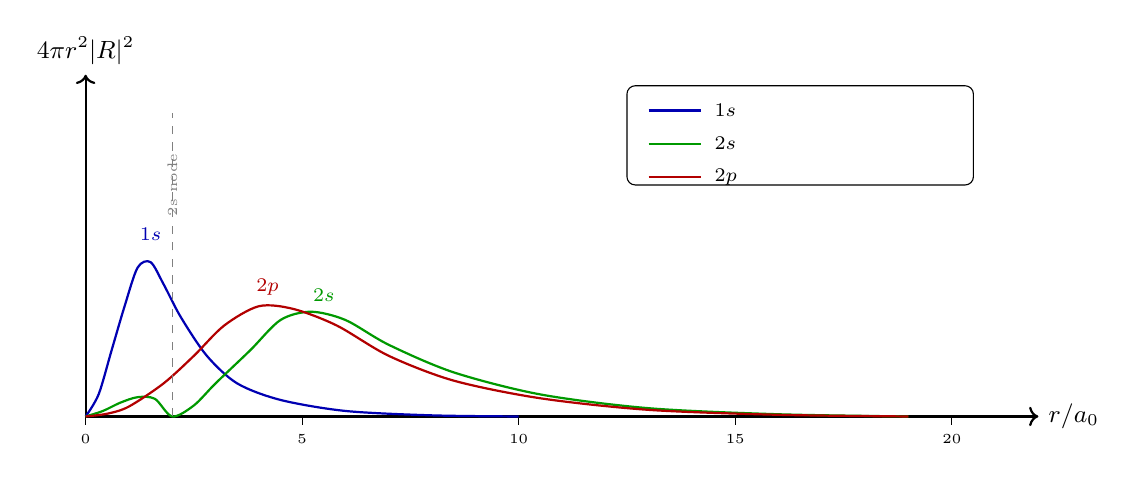
\begin{tikzpicture}[x=0.55cm, y=7cm]

  %% axes
  \draw[->, thick] (0,0) -- (22,0) node[right, font=\small] {$r/a_0$};
  \draw[->, thick] (0,0) -- (0,0.62) node[above, font=\small] {$4\pi r^2|R|^2$};

  %% x-axis ticks
  \foreach \x in {0,5,10,15,20}{
    \draw (\x,0) -- (\x,-0.015) node[below, font=\tiny] {\x};
  }

  %% ---- 1s : peaks at r=1, decays fast ----
  \draw[blue!70!black, thick, tension=0.5]
    plot[smooth] coordinates {
      (0,0)(0.3,0.04)(0.6,0.12)(0.9,0.20)(1.2,0.27)(1.5,0.28)
      (1.8,0.24)(2.2,0.18)(2.8,0.11)(3.5,0.06)(4.5,0.03)
      (6,0.01)(8,0.002)(10,0)
    };
  \node[blue!70!black, font=\scriptsize] at (1.5,0.33) {$1s$};

  %% ---- 2s : small inner peak, node at r=2, big peak at r~5 ----
  \draw[green!60!black, thick, tension=0.5]
    plot[smooth] coordinates {
      (0,0)(0.4,0.01)(0.8,0.025)(1.2,0.035)(1.6,0.032)
      (2.0,0.0)(2.5,0.02)(3.0,0.06)(3.8,0.12)(4.5,0.175)
      (5.2,0.19)(6.0,0.175)(7.0,0.13)(8.5,0.08)(10.5,0.04)
      (13,0.015)(16,0.004)(19,0)
    };
  \node[green!60!black, font=\scriptsize] at (5.5,0.22) {$2s$};

  %% ---- 2p : starts at 0, single broad peak at r~4 ----
  \draw[red!70!black, thick, tension=0.5]
    plot[smooth] coordinates {
      (0,0)(0.5,0.005)(1.0,0.018)(1.8,0.06)(2.5,0.11)
      (3.2,0.165)(4.0,0.20)(4.8,0.195)(5.8,0.165)(7.0,0.11)
      (8.5,0.065)(10.5,0.033)(13,0.012)(16,0.003)(19,0)
    };
  \node[red!70!black, font=\scriptsize] at (4.2,0.235) {$2p$};

  %% ---- node marker for 2s ----
  \draw[dashed, gray, thin] (2.0,0) -- (2.0,0.55);
  \node[gray, font=\tiny, rotate=90] at (2.0,0.42) {2s node};

  %% legend box
  \draw[rounded corners=3pt] (12.5,0.42) rectangle (20.5,0.60);
  \draw[blue!70!black,  thick] (13.0,0.555) -- (14.2,0.555);
  \node[right, font=\scriptsize] at (14.3,0.555) {$1s$};
  \draw[green!60!black, thick] (13.0,0.495) -- (14.2,0.495);
  \node[right, font=\scriptsize] at (14.3,0.495) {$2s$};
  \draw[red!70!black,   thick] (13.0,0.435) -- (14.2,0.435);
  \node[right, font=\scriptsize] at (14.3,0.435) {$2p$};

\end{tikzpicture}
\end{center}

\bigskip
\textbf{1. Analysis of Each Orbital:}

\textbf{(i) 1s orbital} ($n=1,\, l=0$):
\[
  R_{10}(r) = 2\left(\frac{1}{a_0}\right)^{3/2} e^{-r/a_0}
\]
\begin{itemize}
  \item RDF rises steeply from zero, peaks sharply at $r = a_0$ (Bohr radius $= 0.529$ \AA), then decays exponentially.
  \item \textbf{No radial nodes} — $(n - l - 1) = 0$ nodes.
  \item Electron is tightly confined closest to the nucleus.
\end{itemize}

\textbf{(ii) 2s orbital} ($n=2,\, l=0$):
\[
  R_{20}(r) = \frac{1}{2\sqrt{2}}\left(\frac{1}{a_0}\right)^{3/2}\!\left(2 - \frac{r}{a_0}\right)e^{-r/2a_0}
\]
\begin{itemize}
  \item RDF has \textbf{one radial node} at $r = 2a_0$ (where $2 - r/a_0 = 0$), giving \textit{two peaks}: a small inner peak near the nucleus and a larger outer peak around $r \approx 5a_0$.
  \item Number of radial nodes $= (n - l - 1) = 1$.
  \item The \textbf{inner peak} (penetration) gives the 2s electron significant probability density near the nucleus.
\end{itemize}

\textbf{(iii) 2p orbital} ($n=2,\, l=1$):
\[
  R_{21}(r) = \frac{1}{2\sqrt{6}}\left(\frac{1}{a_0}\right)^{3/2}\frac{r}{a_0}\,e^{-r/2a_0}
\]
\begin{itemize}
  \item RDF starts at zero (due to $r/a_0$ factor), rises to a \textbf{single broad peak} around $r \approx 4a_0$, then decays.
  \item \textbf{No radial nodes} — $(n - l - 1) = 0$ nodes.
  \item Has \textbf{one angular node} (nodal plane, $l = 1$), but no inner peak.
  \item The electron has \textit{no significant probability} of being found close to the nucleus.
\end{itemize}

\bigskip
\textbf{2. Nodal Structure Summary:}
\begin{center}
\begin{tabular}{p{1.5cm} p{2cm} p{2.5cm} p{2.5cm} p{2.5cm}}
\toprule
\textbf{Orbital} & \textbf{Radial nodes} & \textbf{Angular nodes} & \textbf{Total nodes} & \textbf{Inner peak?} \\
\midrule
1s & 0 & 0 & 0 & Yes (only peak) \\[3pt]
2s & 1 (at $r=2a_0$) & 0 & 1 & Yes \\[3pt]
2p & 0 & 1 (nodal plane) & 1 & No \\
\bottomrule
\end{tabular}
\end{center}

\bigskip
\textbf{3. Why 2s Electron is Found Closer to Nucleus than 2p:}

Although both 2s and 2p have $n = 2$ and similar average distances from the nucleus, the 2s orbital exhibits a phenomenon called \textbf{penetration}:

\begin{itemize}
  \item The \textbf{inner lobe} of the 2s RDF (before the radial node at $r = 2a_0$) gives the 2s electron a non-negligible probability of being found very close to the nucleus — even inside the 1s shell.
  \item The 2p RDF, by contrast, goes to zero at $r = 0$ (due to the centrifugal barrier from angular momentum, $l = 1$) and has \textit{no} inner peak — it cannot penetrate to the nucleus.
  \item This is quantified by the \textbf{penetration effect}: 2s electrons experience a higher effective nuclear charge $Z_{\text{eff}}$ because they spend more time near the unshielded nucleus:
  \[
    Z_{\text{eff}}(2s) > Z_{\text{eff}}(2p)
  \]
  \item As a consequence, 2s electrons are \textbf{lower in energy} and more tightly bound than 2p electrons — which is why in multi-electron atoms, 2s fills before 2p.
\end{itemize}


\bigskip
\textbf{Conclusion:} The presence of a \textbf{radial node} in the 2s orbital creates an inner probability lobe that allows 2s electrons to \textit{penetrate} closer to the nucleus compared to 2p electrons, which are excluded from the nuclear region by their angular momentum. This penetration difference is the quantum mechanical basis for the 2s--2p energy splitting in multi-electron atoms.
\end{tcolorbox}



\item Evaluate the case of a Ca$^{19+}$ ion with its electron in the 6th excited state: (i) Calculate the longest wavelength of light emitted when the electron transitions to a lower energy level. (ii) Suppose the same transition as in part (i) took place in a hydrogen atom. Would the wavelength of emission be longer than, shorter than, or the same as your answer? \mk{10}
\yr{CHEM 113 | 2023--24}

\begin{tcolorbox}[enhanced,breakable,ansbox,colback=cA!4,colframe=cA,boxrule=0.8pt,arc=5pt,title={\textbf{Answer}},fonttitle=\bfseries\color{white},colbacktitle=cA]
\textbf{Given:}
\begin{itemize}
  \item Ca$^{19+}$ is a \textbf{hydrogenic ion} (one electron) with atomic number $Z = 20$
  \item 6th excited state means $n = 7$ (ground state $n=1$, so excited state
        $n = 1 + 6 = 7$)
  \item Energy of a hydrogenic ion:
  \[
    E_n = -\frac{Z^2 \times 13.6}{n^2} \text{ eV}
  \]
\end{itemize}

\bigskip
\textbf{(i) Longest wavelength of emitted light:}

Longest wavelength $\Rightarrow$ lowest energy transition $\Rightarrow$ smallest
$\Delta E$ $\Rightarrow$ electron drops to the \textbf{nearest lower level},
i.e.\ $n = 7 \rightarrow n = 6$.

\textbf{Calculate $E_7$ and $E_6$:}
\[
  E_7 = -\frac{(20)^2 \times 13.6}{7^2}
      = -\frac{400 \times 13.6}{49}
      = -\frac{5440}{49}
      = -111.02 \text{ eV}
\]
\[
  E_6 = -\frac{(20)^2 \times 13.6}{6^2}
      = -\frac{400 \times 13.6}{36}
      = -\frac{5440}{36}
      = -151.11 \text{ eV}
\]

\textbf{Energy of emitted photon:}
\[
  \Delta E = E_7 - E_6 = -111.02 - (-151.11) = 40.09 \text{ eV}
\]

Converting to Joules:
\[
  \Delta E = 40.09 \times 1.602 \times 10^{-19}
           = 6.422 \times 10^{-18} \text{ J}
\]

\textbf{Wavelength:}
\[
  \lambda = \frac{hc}{\Delta E}
          = \frac{(6.626 \times 10^{-34})(3.0 \times 10^8)}{6.422 \times 10^{-18}}
\]
\[
  \boxed{\lambda = 3.09 \times 10^{-8} \text{ m} = 30.9 \text{ nm}}
\]
This falls in the \textbf{UV region} of the electromagnetic spectrum.

\bigskip
\textbf{(ii) Same transition in hydrogen ($Z = 1$), $n=7 \rightarrow n=6$:}

For hydrogen:
\[
  \Delta E_H = 13.6 \left(\frac{1}{6^2} - \frac{1}{7^2}\right)
             = 13.6 \left(\frac{1}{36} - \frac{1}{49}\right)
             = 13.6 \times \frac{49 - 36}{36 \times 49}
             = 13.6 \times \frac{13}{1764}
             = 0.1003 \text{ eV}
\]

\[
  \lambda_H = \frac{hc}{\Delta E_H}
            = \frac{(6.626\times10^{-34})(3.0\times10^8)}
                   {0.1003 \times 1.602\times10^{-19}}
            = 1.235 \times 10^{-5} \text{ m} = 12{,}350 \text{ nm}
\]

This falls in the \textbf{infrared region}.

\bigskip
\textbf{Comparison:}
\begin{center}
\begin{tabular}{p{3.5cm} p{3cm} p{3cm} p{2.5cm}}
\toprule
\textbf{System} & \textbf{$\Delta E$} & \textbf{$\lambda$} & \textbf{Region} \\
\midrule
Ca$^{19+}$ ($Z=20$) & $40.09$ eV  & $30.9$ nm      & UV \\[3pt]
H ($Z=1$)           & $0.100$ eV  & $12{,}350$ nm  & Infrared \\
\bottomrule
\end{tabular}
\end{center}

The wavelength for hydrogen is \textbf{much longer} than for Ca$^{19+}$.

\textbf{Reason:} The energy of a hydrogenic system scales as $Z^2$:
\[
  \Delta E \propto Z^2 \quad \Longrightarrow \quad \lambda \propto \frac{1}{Z^2}
\]
For Ca$^{19+}$, $Z = 20$, so $\Delta E$ is $20^2 = 400$ times larger than
for hydrogen for the same transition. Since $\lambda = hc/\Delta E$, the
wavelength of Ca$^{19+}$ is 400 times \textit{shorter} than that of hydrogen:
\[
  \frac{\lambda_H}{\lambda_{\text{Ca}^{19+}}} = Z^2 = 400
  \quad \checkmark \quad
  \left(\frac{12350}{30.9} \approx 400\right)
\]

\textbf{Conclusion:} The hydrogen emission wavelength ($12{,}350$ nm, infrared)
is \textbf{far longer} than that of Ca$^{19+}$ ($30.9$ nm, UV) for the same
$n = 7 \rightarrow 6$ transition, because the much higher nuclear charge of
calcium pulls the electron to much lower (more negative) energy levels,
making transitions far more energetic.
\end{tcolorbox}

\item Discuss the periodic trends in ionization energy, electron affinity, atomic size, and metallic properties of elements, illustrating your explanation with the help of a labeled outline of the periodic table. \mk{10}
\yr{CHEM 113 | 2023--24}

\begin{tcolorbox}[enhanced,breakable,ansbox,colback=cA!4,colframe=cA,boxrule=0.8pt,arc=5pt,title={\textbf{Answer}},fonttitle=\bfseries\color{white},colbacktitle=cA]
\textbf{Periodic Trends — Overview:}

Four key periodic properties all depend on \textbf{effective nuclear charge
($Z_{\text{eff}}$)} and \textbf{atomic radius}, and show consistent trends
across periods and down groups.

\bigskip
\textbf{Labeled Periodic Table Showing All Four Trends:}

\begin{center}
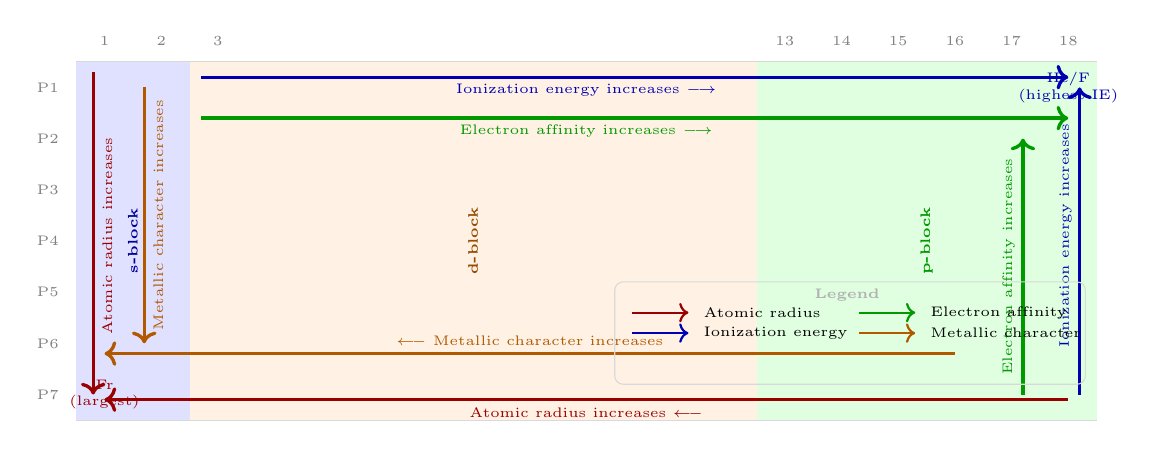
\begin{tikzpicture}[x=0.72cm, y=0.65cm]

  %% ── Period table outline ──────────────────────────────────────
  \draw[gray!30, thin] (0,0) rectangle (18,-7);

  %% Group dividers
  \foreach \x in {1,2,3,4,5,6,7,8,9,10,11,12,13,14,15,16,17}{
    \draw[gray!20, thin] (\x,0) -- (\x,-7);
  }
  %% Period dividers
  \foreach \y in {-1,-2,-3,-4,-5,-6}{
    \draw[gray!20, thin] (0,\y) -- (18,\y);
  }

  %% ── Block fills ───────────────────────────────────────────────
  \fill[blue!12]   (0,0)  rectangle (2,-7);
  \fill[green!12]  (12,0) rectangle (18,-7);
  \fill[orange!10] (2,0)  rectangle (12,-7);

  %% Block labels
  \node[font=\tiny, blue!60!black, rotate=90]   at (1,   -3.5) {\textbf{s-block}};
  \node[font=\tiny, orange!60!black, rotate=90] at (7,   -3.5) {\textbf{d-block}};
  \node[font=\tiny, green!60!black, rotate=90]  at (15,  -3.5) {\textbf{p-block}};

  %% Period labels
  \foreach \y/\p in {0/1,-1/2,-2/3,-3/4,-4/5,-5/6,-6/7}{
    \node[font=\tiny, gray] at (-0.5,{\y-0.5}) {P\p};
  }

  %% Group labels (selected)
  \foreach \x/\g in {0/1,1/2,2/3,12/13,13/14,14/15,15/16,16/17,17/18}{
    \node[font=\tiny, gray] at ({\x+0.5}, 0.4) {\g};
  }

  %% ── Corner element markers ────────────────────────────────────
  \node[font=\tiny, align=center, red!60!black]    at (0.5, -6.5)
    {Fr\\(largest)};
  \node[font=\tiny, align=center, blue!70!black]   at (17.5,-0.5)
    {He/F\\(highest IE)};
  \node[font=\tiny, align=center, green!60!black]  at (16.5,-0.6)
    {};
  \node[font=\tiny, align=center, orange!60!black] at (0.5, -5.8)
    {};

  %% ══════════════════════════════════════════════════════════════
  %%  TREND ARROWS — all kept INSIDE the bounding box (0,0)-(18,-7)
  %% ══════════════════════════════════════════════════════════════

  %% ── Atomic radius (red) ───────────────────────────────────────
  %% decreases left→right  (arrow points right→left = increases)
  \draw[->, very thick, red!60!black]
    (17.5,-6.6) -- (0.5,-6.6);
  \node[font=\tiny, red!60!black] at (9.0,-6.85)
    {Atomic radius increases $\longleftarrow$};

  %% increases top→bottom
  \draw[->, very thick, red!60!black]
    (0.3,-0.2) -- (0.3,-6.5);
  \node[font=\tiny, red!60!black, rotate=90] at (0.55,-3.4)
    {Atomic radius increases};

  %% ── Ionization energy (blue) ──────────────────────────────────
  %% increases left→right
  \draw[->, very thick, blue!70!black]
    (2.2,-0.3) -- (17.5,-0.3);
  \node[font=\tiny, blue!70!black] at (9.0,-0.55)
    {Ionization energy increases $\longrightarrow$};

  %% increases bottom→top
  \draw[->, very thick, blue!70!black]
    (17.7,-6.5) -- (17.7,-0.5);
  \node[font=\tiny, blue!70!black, rotate=90] at (17.45,-3.4)
    {Ionization energy increases};

  %% ── Electron affinity (green) ─────────────────────────────────
  %% increases left→right (inside, slightly below IE arrow)
  \draw[->, very thick, green!60!black]
    (2.2,-1.1) -- (17.5,-1.1);
  \node[font=\tiny, green!60!black] at (9.0,-1.35)
    {Electron affinity increases $\longrightarrow$};

  %% increases bottom→top
  \draw[->, very thick, green!60!black]
    (16.7,-6.5) -- (16.7,-1.5);
  \node[font=\tiny, green!60!black, rotate=90] at (16.45,-4.0)
    {Electron affinity increases};

  %% ── Metallic character (orange) ───────────────────────────────
  %% increases right→left
  \draw[->, very thick, orange!70!black]
    (15.5,-5.7) -- (0.5,-5.7);
  \node[font=\tiny, orange!70!black] at (8.0,-5.45)
    {$\longleftarrow$ Metallic character increases};

  %% increases top→bottom
  \draw[->, very thick, orange!70!black]
    (1.2,-0.5) -- (1.2,-5.5);
  \node[font=\tiny, orange!70!black, rotate=90] at (1.45,-3.0)
    {Metallic character increases};

  %% ── Legend (inside box, bottom-right) ────────────────────────
  \draw[rounded corners=3pt, gray!30] (9.5,-4.3) rectangle (17.8,-6.3);
  \node[font=\tiny\bfseries, gray!60] at (13.6,-4.55) {Legend};

  \draw[red!60!black,   ->, thick] (9.8,-4.9)  -- (10.8,-4.9);
  \node[right, font=\tiny] at (10.9,-4.9)  {Atomic radius};

  \draw[blue!70!black,  ->, thick] (9.8,-5.3)  -- (10.8,-5.3);
  \node[right, font=\tiny] at (10.9,-5.3)  {Ionization energy};

  \draw[green!60!black, ->, thick] (13.8,-4.9) -- (14.8,-4.9);
  \node[right, font=\tiny] at (14.9,-4.9)  {Electron affinity};

  \draw[orange!70!black,->, thick] (13.8,-5.3) -- (14.8,-5.3);
  \node[right, font=\tiny] at (14.9,-5.3)  {Metallic character};

\end{tikzpicture}
\end{center}

\bigskip
\textbf{1. Ionization Energy (IE):}

IE is the energy required to remove the outermost electron from a
gaseous atom:
\[
  \text{M}_{(g)} \rightarrow \text{M}^+_{(g)} + e^-
\]
\begin{itemize}
  \item \textbf{Across a period} ($\rightarrow$): $Z_{\text{eff}}$
        increases, electrons are held more tightly $\Rightarrow$
        \textbf{IE increases}.
        Exception: slight dip at group 3 (e.g.\ Al $<$ Mg) due to
        $2p$ being higher than $2s$, and at group 6 (e.g.\ S $<$ P)
        due to pairing repulsion.
  \item \textbf{Down a group} ($\downarrow$): atomic radius increases,
        outer electron farther from nucleus, more shielded
        $\Rightarrow$ \textbf{IE decreases}.
  \item Highest IE: He ($2372$ kJ/mol); Lowest: Cs ($376$ kJ/mol).
\end{itemize}

\bigskip
\textbf{2. Electron Affinity (EA):}

EA is the energy change when a gaseous atom gains one electron:
\[
  \text{M}_{(g)} + e^- \rightarrow \text{M}^-_{(g)}
\]
\begin{itemize}
  \item \textbf{Across a period} ($\rightarrow$): increasing
        $Z_{\text{eff}}$ makes atoms more attractive to electrons
        $\Rightarrow$ \textbf{EA becomes more negative} (more
        favourable). Exception: group 2 (filled $s$) and group 5
        (half-filled $p$) show anomalously low EA.
  \item \textbf{Down a group} ($\downarrow$): larger radius, increased
        shielding $\Rightarrow$ \textbf{EA decreases} (less favourable).
        Exception: F $<$ Cl due to electron--electron repulsion in the
        compact $2p$ orbital.
  \item Most negative EA: Cl ($-349$ kJ/mol).
\end{itemize}

\bigskip
\textbf{3. Atomic Size (Atomic Radius):}

\begin{itemize}
  \item \textbf{Across a period} ($\rightarrow$): increasing $Z$
        pulls electrons closer with little extra shielding
        $\Rightarrow$ \textbf{radius decreases}.
  \item \textbf{Down a group} ($\downarrow$): new electron shells
        are added, greatly increasing shielding $\Rightarrow$
        \textbf{radius increases}.
  \item Largest atom: Fr ($\sim$270 pm);
        Smallest: He ($\sim$31 pm).
\end{itemize}

\bigskip
\textbf{4. Metallic Character:}

Metallic character reflects the tendency to \textbf{lose electrons}
and form cations — linked directly to low IE and large atomic radius.
\begin{itemize}
  \item \textbf{Across a period} ($\rightarrow$): IE increases,
        electron loss becomes harder $\Rightarrow$ \textbf{metallic
        character decreases} (metals on left, non-metals on right).
  \item \textbf{Down a group} ($\downarrow$): IE decreases, electrons
        lost more easily $\Rightarrow$ \textbf{metallic character
        increases}.
  \item Most metallic: Fr (bottom-left);
        Least metallic: F/He (top-right).
\end{itemize}

\bigskip
\textbf{Summary Table:}
\begin{center}
\begin{tabular}{p{3.2cm} p{3.0cm} p{3.0cm}}
\toprule
\textbf{Property} & \textbf{Across period} ($\rightarrow$) &
\textbf{Down group} ($\downarrow$) \\
\midrule
Ionization energy   & Increases   & Decreases \\[3pt]
Electron affinity   & More negative & Less negative \\[3pt]
Atomic radius       & Decreases   & Increases \\[3pt]
Metallic character  & Decreases   & Increases \\
\bottomrule
\end{tabular}
\end{center}

\textbf{Conclusion:} All four trends are governed by the interplay of
\textbf{nuclear charge}, \textbf{shielding}, and \textbf{atomic radius}.
Increasing $Z_{\text{eff}}$ (across a period) tightens electron
hold, raising IE and EA while shrinking the atom and reducing metallic
character. Increasing shielding (down a group) has the opposite effect,
making valence electrons easier to remove and atoms more metallic.
\end{tcolorbox}


\item Consider a photoelectric experiment in which light of variable frequency strikes a metal surface. Plot the kinetic energy of emitted electrons as a function of the frequency of the incident light. From this graph, derive the work function of the metal, and discuss how the graph would differ if the light source were replaced with a source of lower frequency which is below the threshold frequency. \mk{10}
\yr{CHEM 113 | 2022--23}

\begin{tcolorbox}[enhanced,breakable,ansbox,colback=cA!4,colframe=cA,boxrule=0.8pt,arc=5pt,title={\textbf{Answer}},fonttitle=\bfseries\color{white},colbacktitle=cA]

\textbf{Photoelectric Effect: KE vs.\ Frequency Graph \& Work Function}
\hfill \mk{10}

\medskip
\begin{center}
\textcolor{cA}{\rule{0.85\textwidth}{0.5pt}}
\end{center}

%% ── Part 1 ────────────────────────────────────────────────────────────
\medskip
\textbf{Part 1: The KE vs.\ Frequency Graph} \hfill \mk{3}

\medskip
From Einstein's photoelectric equation:
\[
  \frac{1}{2}mv^2_{\max} = h\nu - \phi = h\nu - h\nu_0 = h(\nu - \nu_0)
\]
Plotting KE$_{\max}$ on the $y$-axis against frequency $\nu$ on the $x$-axis
gives a \textbf{straight line} with:
\[
  \underbrace{\text{slope} = h}_{\text{Planck's constant}}
  \qquad
  \underbrace{x\text{-intercept} = \nu_0}_{\text{threshold frequency}}
  \qquad
  \underbrace{y\text{-intercept} = -\phi}_{\text{(negative work function)}}
\]

\begin{center}
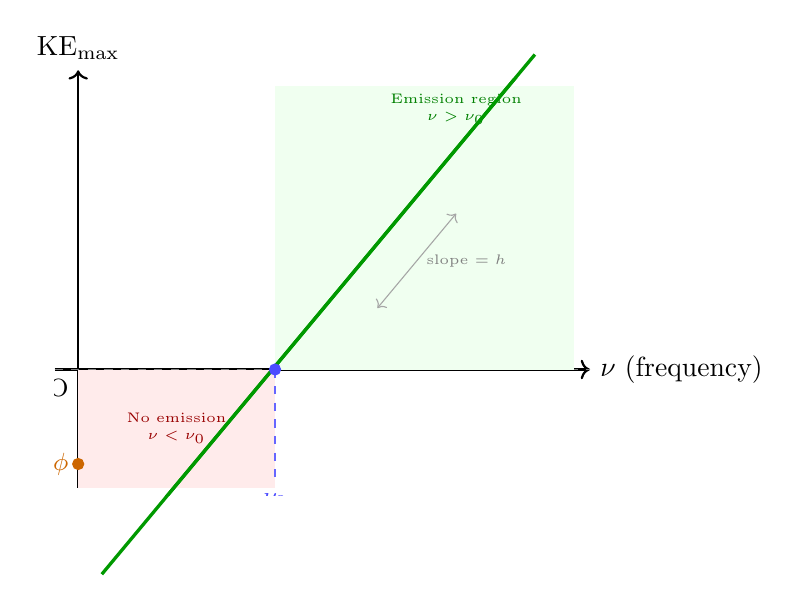
\begin{tikzpicture}[scale=1.0]
  %% Axes
  \draw[->, thick] (-0.3, 0) -- (6.5, 0) node[right] {$\nu$ (frequency)};
  \draw[->, thick] (0, -1.5) -- (0, 3.8)
        node[above] {KE$_{\max}$};

  %% Zero line label
  \draw[dashed, gray] (-0.3,0) -- (6.5,0);

  %% No-emission region shading
  \fill[red!8] (0,-1.5) rectangle (2.5,0);
  \node[font=\tiny, text=red!60!black, align=center] at (1.25,-0.75)
        {No emission\\$\nu < \nu_0$};

  %% Emission region shading
  \fill[green!6] (2.5,0) rectangle (6.3,3.6);
  \node[font=\tiny, text=green!50!black, align=center] at (4.8, 3.3)
        {Emission region\\$\nu > \nu_0$};

  %% Main line: passes through (2.5,0) with slope ~1.2
  \draw[green!60!black, very thick] (0.3,-2.6) -- (5.8, 4.0);
  %% Clip the line to visible area by only drawing in range
  \clip (-0.3,-1.6) rectangle (6.5,3.7);
  \draw[green!60!black, very thick] (0.3,-2.6) -- (5.8, 4.0);

  %% Threshold frequency marker
  \draw[dashed, blue!60] (2.5, 0) -- (2.5, -1.4);
  \filldraw[blue!70] (2.5, 0) circle (2pt);
  \node[below, font=\small, text=blue!70] at (2.5,-1.45) {$\nu_0$};

  %% y-intercept marker (negative phi)
  \filldraw[orange!80!black] (0,-1.2) circle (2pt);
  \node[left, font=\small, text=orange!80!black] at (0,-1.2) {$-\phi$};

  %% Slope annotation
  \draw[<->, gray!70, thin]
        (3.8, 0.78) -- (4.8, 1.98)
        node[midway, right, font=\tiny, text=gray] {slope $= h$};

  %% Origin
  \node[below left, font=\small] at (0,0) {O};
\end{tikzpicture}
\end{center}

\begin{center}
\textcolor{cA}{\rule{0.75\textwidth}{0.4pt}}
\end{center}

%% ── Part 2 ────────────────────────────────────────────────────────────
\medskip
\textbf{Part 2: Deriving the Work Function from the Graph} \hfill \mk{4}

\medskip
The Einstein photoelectric equation is a straight line of the form
$y = mx + c$:
\[
  \text{KE}_{\max} = h\nu - \phi
  \quad\longleftrightarrow\quad
  y = \underbrace{h}_{\text{slope}}\cdot\nu
    + \underbrace{(-\phi)}_{y\text{-intercept}}
\]

\textbf{Method 1 --- From the $x$-intercept:}

At the threshold frequency $\nu_0$, KE$_{\max} = 0$. Setting KE $= 0$:
\[
  0 = h\nu_0 - \phi
  \qquad\Rightarrow\qquad
  \boxed{\phi = h\nu_0}
\]
So the work function equals Planck's constant multiplied by the
$x$-intercept read directly off the graph.

\medskip
\textbf{Method 2 --- From the $y$-intercept:}

Extrapolating the straight line back to the $y$-axis gives a negative
intercept. The magnitude of this intercept is directly equal to $\phi$:
\[
  \phi = \big|y\text{-intercept}\big|
\]

\medskip
\textbf{Method 3 --- From the slope:}

The slope of the line equals $h$ (Planck's constant). Once the slope is
measured experimentally, and two points $(\nu_1,\, \text{KE}_1)$ and
$(\nu_2,\, \text{KE}_2)$ are known:
\[
  h = \frac{\Delta\,\text{KE}}{\Delta\nu}
  = \frac{\text{KE}_2 - \text{KE}_1}{\nu_2 - \nu_1}
  \qquad\Rightarrow\qquad
  \phi = h\nu - \text{KE at any known point}
\]

\begin{center}
\textcolor{cA}{\rule{0.75\textwidth}{0.4pt}}
\end{center}

%% ── Part 3 ────────────────────────────────────────────────────────────
\medskip
\textbf{Part 3: Effect of Replacing with a Sub-threshold Light Source}
\hfill \mk{3}

\medskip
If the incident light has frequency $\nu < \nu_0$ (below the threshold):

\begin{itemize}[leftmargin=1.5em, itemsep=4pt]
  \item \textbf{No electrons are emitted} --- regardless of how intense
        the light source is or how long it illuminates the surface.
  \item Each photon carries energy $h\nu < \phi$, so no single photon
        has sufficient energy to overcome the work function and free
        an electron.
  \item \textbf{The graph does not extend} into the positive KE region.
        The entire operating range lies to the \emph{left} of $\nu_0$,
        where KE $= 0$ for all frequencies.
  \item \textbf{No straight line is observed} --- instead, the KE axis
        remains flat at zero for all $\nu < \nu_0$, as illustrated below:
\end{itemize}

\begin{center}
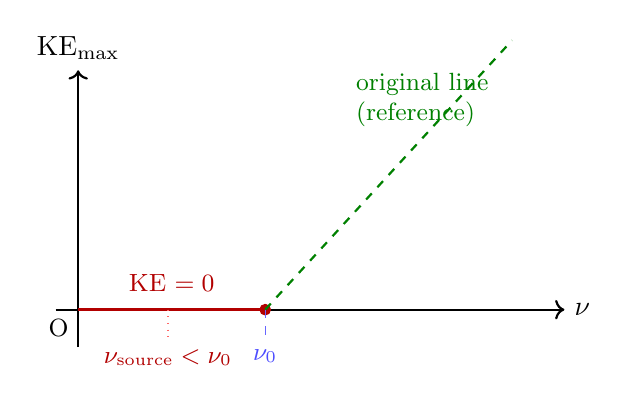
\begin{tikzpicture}[scale=0.95]
  \draw[->, thick] (-0.3,0) -- (6.5,0) node[right] {$\nu$};
  \draw[->, thick] (0,-0.5) -- (0, 3.2) node[above] {KE$_{\max}$};

  %% Flat zero line for sub-threshold region
  \draw[red!70!black, very thick] (0,0) -- (2.5,0);
  \filldraw[red!70!black] (2.5,0) circle (2pt);

  %% Ghost of original line (dashed)
  \draw[green!50!black, thick, dashed] (2.5,0) -- (5.8,3.6);

  %% Sub-threshold source marker
  \draw[dotted, red!60] (1.2,0) -- (1.2,-0.4);
  \node[below, font=\small, text=red!70!black] at (1.2,-0.4)
        {$\nu_{\text{source}} < \nu_0$};

  %% Threshold
  \draw[dashed, blue!60] (2.5,0) -- (2.5,-0.4);
  \node[below, font=\small, text=blue!70] at (2.5,-0.4) {$\nu_0$};

  %% Labels
  \node[font=\small, text=red!70!black] at (1.25, 0.35)
        {KE $= 0$};
  \node[font=\small, text=green!50!black, align=left] at (4.6, 2.8)
        {original line\\(reference)};
  \node[below left, font=\small] at (0,0) {O};
\end{tikzpicture}
\end{center}

The red flat line shows that the sub-threshold source produces
\emph{zero} kinetic energy for all frequencies up to $\nu_0$.
The dashed green line is the original graph shown for reference.
This stark contrast demonstrates that the photoelectric effect is
\textbf{not} a gradual phenomenon --- it has a sharp, well-defined
cutoff at $\nu_0$.

\medskip
\begin{center}
\textcolor{cA}{\rule{0.85\textwidth}{0.5pt}}
\end{center}

\medskip
\textbf{Conclusion:} The KE vs.\ $\nu$ graph is a powerful tool ---
its slope gives Planck's constant $h$, its $x$-intercept gives $\nu_0$,
and its $y$-intercept gives $-\phi$. A sub-threshold source produces no
graph at all in the positive KE region, confirming that photon energy
must exceed $\phi$ for any emission to occur.

\end{tcolorbox}

\item Inside an atom, the uncertainty in the position of an electron is 0.1 nm. Calculate the minimum uncertainty in the momentum of the particle. If the electron has a de Broglie wavelength $\lambda = 2.0 \times 10^{-10}$ m, calculate its velocity and discuss how the uncertainty in the particle's position influences its momentum and velocity. \mk{10}
\yr{CHEM 113 | 2022--23}

\begin{tcolorbox}[enhanced,breakable,ansbox,colback=cA!4,colframe=cA,boxrule=0.8pt,arc=5pt,title={\textbf{Answer}},fonttitle=\bfseries\color{white},colbacktitle=cA]

\textbf{Heisenberg Uncertainty \& de Broglie Wavelength of an Electron}
\hfill \mk{10}

\medskip
\begin{center}
\textcolor{cA}{\rule{0.85\textwidth}{0.5pt}}
\end{center}

%% ── Part 1 ────────────────────────────────────────────────────────────
\medskip
\textbf{Part 1: Minimum Uncertainty in Momentum} \hfill \mk{3}

\medskip
Heisenberg's Uncertainty Principle states that the position and momentum of
a particle cannot both be known precisely at the same time:
\[
  \Delta x \cdot \Delta p \;\geq\; \frac{h}{4\pi}
\]
For \emph{minimum} uncertainty, we use the equality:
\[
  \Delta p_{\min} = \frac{h}{4\pi\,\Delta x}
\]

\textbf{Given:} $\Delta x = 0.1$ nm $= 0.1 \times 10^{-9}$ m
$= 1.0 \times 10^{-10}$ m

\medskip
Substituting:
\[
  \Delta p_{\min}
  = \frac{6.626 \times 10^{-34}}{4\pi \times 1.0 \times 10^{-10}}
  = \frac{6.626 \times 10^{-34}}{1.2566 \times 10^{-9}}
\]
\[
  \boxed{\Delta p_{\min} = 5.27 \times 10^{-25} \text{ kg$\cdot$m/s}}
\]

\begin{center}
\textcolor{cA}{\rule{0.75\textwidth}{0.4pt}}
\end{center}

%% ── Part 2 ────────────────────────────────────────────────────────────
\medskip
\textbf{Part 2: Velocity from de Broglie Wavelength} \hfill \mk{3}

\medskip
The de Broglie relation connects wavelength to momentum:
\[
  \lambda = \frac{h}{mv}
  \qquad\Rightarrow\qquad
  v = \frac{h}{m\lambda}
\]

\textbf{Given:}
$\lambda = 2.0 \times 10^{-10}$ m,\quad
$m_e = 9.109 \times 10^{-31}$ kg

\medskip
Substituting:
\[
  v = \frac{6.626 \times 10^{-34}}{9.109 \times 10^{-31}
      \times 2.0 \times 10^{-10}}
  = \frac{6.626 \times 10^{-34}}{1.822 \times 10^{-40}}
\]
\[
  \boxed{v = 3.64 \times 10^{6} \text{ m/s}}
\]

This is approximately $1.2\%$ of the speed of light --- confirming the
electron is moving at a highly energetic but still non-relativistic speed.

\begin{center}
\textcolor{cA}{\rule{0.75\textwidth}{0.4pt}}
\end{center}

%% ── Part 3 ────────────────────────────────────────────────────────────
\medskip
\textbf{Part 3: How Uncertainty in Position Influences
Momentum \& Velocity} \hfill \mk{4}

\medskip
\textbf{(i) The Inverse Relationship:}

From the uncertainty principle $\Delta x \cdot \Delta p \geq h/4\pi$,
position uncertainty $\Delta x$ and momentum uncertainty $\Delta p$ are
\emph{inversely} related:
\[
  \Delta p \;\propto\; \frac{1}{\Delta x}
\]

\begin{center}
\begin{tabular}{p{0.28\textwidth} p{0.28\textwidth} p{0.28\textwidth}}
\toprule
\textbf{Situation} & \textbf{$\Delta x$} & \textbf{$\Delta p$} \\
\midrule
Position known precisely & Very small & Very large \\
Position poorly known    & Very large & Very small \\
Balanced (atomic scale)  & $\sim 10^{-10}$ m & $\sim 10^{-25}$ kg$\cdot$m/s \\
\bottomrule
\end{tabular}
\end{center}

\medskip
\textbf{(ii) Influence on Momentum:}

Since $p = mv$ and $m$ is fixed for an electron, the uncertainty in
momentum directly translates to uncertainty in velocity:
\[
  \Delta p = m_e\,\Delta v
  \qquad\Rightarrow\qquad
  \Delta v = \frac{\Delta p}{m_e}
  = \frac{5.27 \times 10^{-25}}{9.109 \times 10^{-31}}
  \approx 5.79 \times 10^{5} \text{ m/s}
\]
This means the velocity is uncertain by about $5.79 \times 10^5$ m/s ---
roughly \textbf{16\%} of the calculated velocity $v = 3.64 \times 10^6$
m/s. This is a significant uncertainty, not a negligible one.

\medskip
\textbf{(iii) Physical Interpretation:}

\begin{itemize}[leftmargin=1.5em, itemsep=3pt]
  \item Confining an electron to a small region (small $\Delta x$, as inside
        an atom) \emph{forces} a large spread in its momentum $\Delta p$ ---
        the electron cannot be at rest; it must be in vigorous motion.
  \item This is why electrons do \emph{not} collapse into the nucleus despite
        electrostatic attraction --- confinement to the nucleus
        ($\Delta x \sim 10^{-15}$ m) would require an impossibly large
        momentum uncertainty.
  \item Unlike macroscopic objects, for an electron at the atomic scale
        ($\Delta x \sim 10^{-10}$ m), the uncertainty $\Delta v \sim
        10^5$--$10^6$ m/s is comparable to the actual velocity --- making
        a precise classical trajectory \emph{physically meaningless}.
  \item This is precisely why quantum mechanics replaces the concept of a
        definite orbit (Bohr) with a \textbf{probability cloud} --- the
        electron's position and momentum are fundamentally uncertain
        simultaneously.
\end{itemize}

\medskip
\begin{center}
\textcolor{cA}{\rule{0.85\textwidth}{0.5pt}}
\end{center}

\medskip
\textbf{Conclusion:} The minimum momentum uncertainty is
$5.27 \times 10^{-25}$ kg$\cdot$m/s and the electron velocity from the
de~Broglie wavelength is $3.64 \times 10^6$ m/s. The resulting velocity
uncertainty of $\sim 16\%$ confirms that at the atomic scale, the
Heisenberg principle is not a measurement limitation --- it is a
fundamental property of nature that makes classical trajectory
descriptions impossible.

\end{tcolorbox}

\item Sketch the wave functions and the probabilities for 3s, 3p, and 4s orbitals. \mk{5}
\yr{CHEM 113 | 2022--23}

\begin{tcolorbox}[enhanced,breakable,ansbox,colback=cA!4,colframe=cA,boxrule=0.8pt,arc=5pt,title={\textbf{Answer}},fonttitle=\bfseries\color{white},colbacktitle=cA]

\textbf{Wave Functions $\psi(r)$ and Probability Distributions $4\pi r^2|\psi|^2$
for 3s, 3p, and 4s orbitals:}

\begin{center}
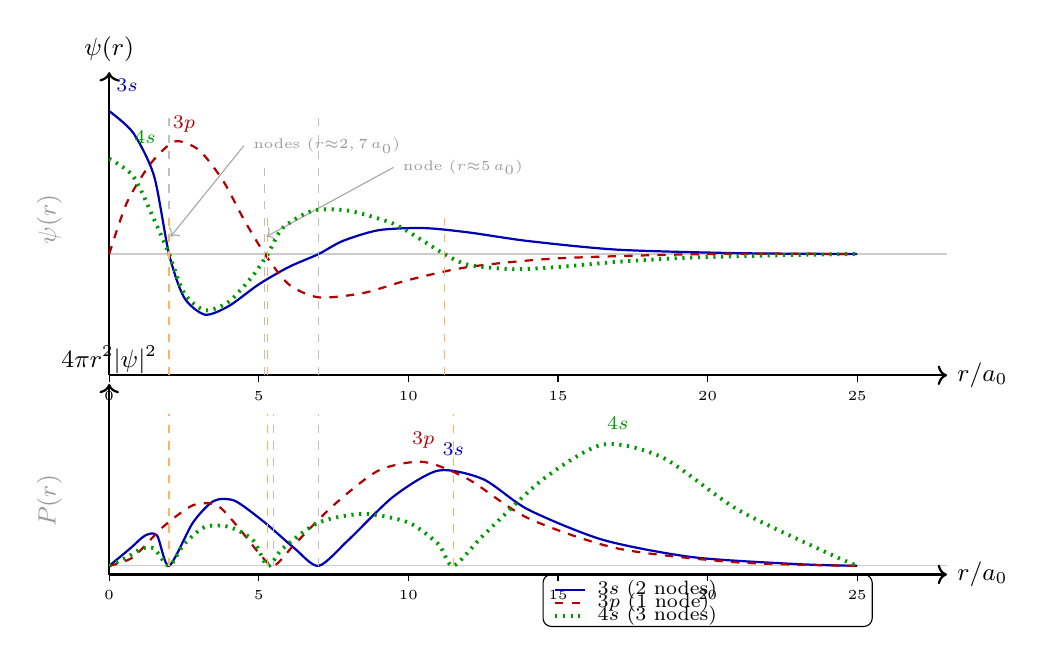
\begin{tikzpicture}[x=0.38cm, y=5.5cm]

  %% ============================================================
  %%  TOP HALF — Wave functions psi(r)
  %% ============================================================

  %% y=0 is the zero-line for psi plots
  \draw[gray!40, thin] (0,0) -- (28,0);

  %% axes
  \draw[->, thick] (0,-0.28) -- (0, 0.42)
    node[above, font=\small] {$\psi(r)$};
  \draw[->, thick] (0,-0.28) -- (28,-0.28)
    node[right, font=\small] {$r/a_0$};
  \foreach \x in {0,5,10,15,20,25}{
    \draw (\x,-0.28) -- (\x,-0.295)
      node[below, font=\tiny] {\x};
  }

  %% --- 3s wavefunction (2 radial nodes: r~2, r~7) ---
  \draw[blue!70!black, thick]
    plot[smooth, tension=0.45] coordinates {
      (0, 0.33)
      (0.8, 0.28)(1.5, 0.18)(2.0, 0.0)
      (2.5,-0.10)(3.2,-0.14)(4.0,-0.12)(5.0,-0.07)
      (6.0,-0.03)(7.0, 0.0)
      (7.8, 0.03)(9.0, 0.055)(10.5,0.06)(12.0,0.05)
      (14.0,0.03)(17.0,0.01)(21.0,0.002)(25,0)
    };
  \node[blue!70!black, font=\scriptsize] at (0.6,0.39) {$3s$};

  %% node markers for 3s
  \draw[dashed, gray!50, thin] (2.0,-0.28) -- (2.0, 0.33);
  \draw[dashed, gray!50, thin] (7.0,-0.28) -- (7.0, 0.33);
  \draw[->, gray!70, thin] (4.5, 0.25)
    node[right, font=\tiny, gray!80] {nodes ($r{\approx}2,7\,a_0$)}
    -- (2.05, 0.04);

  %% --- 3p wavefunction (1 radial node: r~5) ---
  \draw[red!70!black, thick, dashed]
    plot[smooth, tension=0.45] coordinates {
      (0, 0.0)
      (0.6, 0.12)(1.4, 0.21)(2.2, 0.26)(3.0, 0.24)
      (3.8, 0.17)(4.5, 0.08)(5.2, 0.0)
      (6.0,-0.07)(7.0,-0.10)(8.5,-0.09)(10.0,-0.06)
      (12.0,-0.03)(15.0,-0.01)(20.0,0)(25,0)
    };
  \node[red!70!black, font=\scriptsize] at (2.5,0.30) {$3p$};

  %% node marker for 3p
  \draw[dashed, gray!50, thin] (5.2,-0.28) -- (5.2, 0.20);
  \draw[->, gray!70, thin] (9.5, 0.20)
    node[right, font=\tiny, gray!80] {node ($r{\approx}5\,a_0$)}
    -- (5.25, 0.04);

  %% --- 4s wavefunction (3 radial nodes: r~2, r~5, r~11) ---
  \draw[green!60!black, thick, dotted, line width=1.4pt]
    plot[smooth, tension=0.45] coordinates {
      (0, 0.22)
      (0.8, 0.18)(1.5, 0.08)(2.0, 0.0)
      (2.5,-0.09)(3.2,-0.13)(4.0,-0.11)(4.8,-0.05)
      (5.3, 0.0)
      (5.8, 0.06)(6.8, 0.10)(8.0, 0.10)(9.5, 0.07)
      (10.5,0.03)(11.2, 0.0)
      (12.0,-0.025)(13.5,-0.035)(15.0,-0.030)(17.0,-0.018)
      (19.5,-0.008)(23.0,-0.002)(25,0)
    };
  \node[green!60!black, font=\scriptsize] at (1.2,0.27) {$4s$};

  %% node markers for 4s
  \draw[dashed, orange!60, thin] (2.0,-0.28)  -- (2.0,  0.10);
  \draw[dashed, orange!60, thin] (5.3,-0.28)  -- (5.3,  0.10);
  \draw[dashed, orange!60, thin] (11.2,-0.28) -- (11.2, 0.10);

  %% ============================================================
  %%  BOTTOM HALF — Probability distributions 4pi r^2 psi^2
  %% ============================================================
  \def\yoff{-0.72}   %% shift down for probability panel

  %% zero line and axes
  \draw[gray!40, thin] (0,\yoff) -- (28,\yoff);
  \draw[->, thick] (0,{\yoff-0.02}) -- (0,{\yoff+0.42})
    node[above, font=\small] {$4\pi r^2|\psi|^2$};
  \draw[->, thick] (0,{\yoff-0.02}) -- (28,{\yoff-0.02})
    node[right, font=\small] {$r/a_0$};
  \foreach \x in {0,5,10,15,20,25}{
    \draw (\x,{\yoff-0.02}) -- (\x,{\yoff-0.035})
      node[below, font=\tiny] {\x};
  }

  %% --- 3s RDF (3 peaks separated by 2 nodes) ---
  \draw[blue!70!black, thick]
    plot[smooth, tension=0.45] coordinates {
      (0,\yoff)
      (0.7,{\yoff+0.04})(1.2,{\yoff+0.07})(1.6,{\yoff+0.07})
      (2.0,\yoff)
      (2.8,{\yoff+0.10})(3.5,{\yoff+0.15})(4.2,{\yoff+0.15})
      (5.2,{\yoff+0.10})(6.2,{\yoff+0.04})
      (7.0,\yoff)
      (8.0,{\yoff+0.06})(9.5,{\yoff+0.16})(11.0,{\yoff+0.22})
      (12.5,{\yoff+0.20})(14.0,{\yoff+0.13})(16.5,{\yoff+0.06})
      (19.5,{\yoff+0.02})(23,{\yoff+0.004})(25,\yoff)
    };
  \node[blue!70!black, font=\scriptsize] at (11.5,{\yoff+0.27}) {$3s$};

  %% node markers for 3s RDF
  \draw[dashed, gray!50, thin]
    (2.0,\yoff) -- (2.0,{\yoff+0.35});
  \draw[dashed, gray!50, thin]
    (7.0,\yoff) -- (7.0,{\yoff+0.35});

  %% --- 3p RDF (2 peaks, 1 node) ---
  \draw[red!70!black, thick, dashed]
    plot[smooth, tension=0.45] coordinates {
      (0,\yoff)
      (0.8,{\yoff+0.02})(1.8,{\yoff+0.09})(2.8,{\yoff+0.14})
      (3.6,{\yoff+0.14})(4.3,{\yoff+0.09})(5.0,{\yoff+0.03})
      (5.5,\yoff)
      (6.2,{\yoff+0.05})(7.5,{\yoff+0.14})(9.0,{\yoff+0.22})
      (10.5,{\yoff+0.24})(12.0,{\yoff+0.20})(14.0,{\yoff+0.11})
      (17.0,{\yoff+0.04})(21.0,{\yoff+0.008})(25,\yoff)
    };
  \node[red!70!black, font=\scriptsize] at (10.5,{\yoff+0.29}) {$3p$};

  %% node marker for 3p RDF
  \draw[dashed, gray!50, thin]
    (5.5,\yoff) -- (5.5,{\yoff+0.35});

  %% --- 4s RDF (4 peaks, 3 nodes) ---
  \draw[green!60!black, thick, dotted, line width=1.4pt]
    plot[smooth, tension=0.45] coordinates {
      (0,\yoff)
      (0.6,{\yoff+0.02})(1.1,{\yoff+0.04})(1.5,{\yoff+0.04})
      (2.0,\yoff)
      (2.5,{\yoff+0.05})(3.2,{\yoff+0.09})(4.0,{\yoff+0.09})
      (4.8,{\yoff+0.06})(5.3,\yoff)
      (5.8,{\yoff+0.04})(7.0,{\yoff+0.10})(8.5,{\yoff+0.12})
      (10.0,{\yoff+0.10})(11.0,{\yoff+0.05})(11.5,\yoff)
      (12.5,{\yoff+0.07})(14.5,{\yoff+0.20})(16.5,{\yoff+0.28})
      (18.5,{\yoff+0.25})(21.0,{\yoff+0.13})(24.0,{\yoff+0.03})
      (25,\yoff)
    };
  \node[green!60!black, font=\scriptsize] at (17.0,{\yoff+0.33}) {$4s$};

  %% node markers for 4s RDF
  \draw[dashed, orange!60, thin]
    (2.0,\yoff)  -- (2.0, {\yoff+0.35});
  \draw[dashed, orange!60, thin]
    (5.3,\yoff)  -- (5.3, {\yoff+0.35});
  \draw[dashed, orange!60, thin]
    (11.5,\yoff) -- (11.5,{\yoff+0.35});

  %% ---- shared legend ----
  \draw[rounded corners=3pt] (14.5,{\yoff-0.14}) rectangle (25.5,{\yoff-0.02});
  \draw[blue!70!black, thick]
    (14.9,{\yoff-0.055}) -- (15.9,{\yoff-0.055});
  \node[right, font=\scriptsize] at (16.0,{\yoff-0.055})
    {$3s$\ (2 nodes)};
  \draw[red!70!black, thick, dashed]
    (14.9,{\yoff-0.085}) -- (15.9,{\yoff-0.085});
  \node[right, font=\scriptsize] at (16.0,{\yoff-0.085})
    {$3p$\ (1 node)};
  \draw[green!60!black, thick, dotted, line width=1.4pt]
    (14.9,{\yoff-0.115}) -- (15.9,{\yoff-0.115});
  \node[right, font=\scriptsize] at (16.0,{\yoff-0.115})
    {$4s$\ (3 nodes)};

  %% panel labels
  \node[font=\small\bfseries, gray!80] at (-2.0, 0.08)
    {\rotatebox{90}{$\psi(r)$}};
  \node[font=\small\bfseries, gray!80] at (-2.0,{\yoff+0.15})
    {\rotatebox{90}{$P(r)$}};

\end{tikzpicture}
\end{center}

\bigskip
\textbf{Key Features Summary:}
\begin{center}
\begin{tabular}{p{1.5cm} p{2.2cm} p{2.2cm} p{2.2cm} p{3cm}}
\toprule
\textbf{Orbital} & \textbf{Radial nodes} $(n{-}l{-}1)$ &
\textbf{Angular nodes} $(l)$ & \textbf{RDF peaks} &
\textbf{Sign changes in $\psi$} \\
\midrule
$3s$ & 2 & 0 & 3 & 2 (at $r{\approx}2,\,7\,a_0$) \\[3pt]
$3p$ & 1 & 1 & 2 & 1 (at $r{\approx}5\,a_0$) \\[3pt]
$4s$ & 3 & 0 & 4 & 3 (at $r{\approx}2,\,5,\,11\,a_0$) \\
\bottomrule
\end{tabular}
\end{center}

\textbf{Note:} The $\psi(r)$ plots show sign changes at each radial node.
The RDF $4\pi r^2|\psi|^2$ is always non-negative and touches zero at
each radial node. The 4s orbital, having more nodes than 3s and 3p,
has greater penetration toward the nucleus — explaining why
$E_{4s} < E_{3d}$ in multi-electron atoms.

\end{tcolorbox}

\item Demonstrate the relationship between blackbody radiation and Planck's quantum theory. \mk{10}
\yr{CHEM 113 | 2021--22}

\begin{tcolorbox}[enhanced,breakable,ansbox,colback=cA!4,colframe=cA,boxrule=0.8pt,arc=5pt,title={\textbf{Answer}},fonttitle=\bfseries\color{white},colbacktitle=cA]

\textbf{Blackbody Radiation \& Planck's Quantum Theory} \hfill \mk{10}

\medskip
\begin{center}
\textcolor{cA}{\rule{0.85\textwidth}{0.5pt}}
\end{center}

%% ── Part 1 ────────────────────────────────────────────────────────────
\medskip
\textbf{Part 1: What is Blackbody Radiation?} \hfill \mk{2}

\medskip
A \textbf{blackbody} is an ideal object that:
\begin{itemize}[leftmargin=1.5em, itemsep=2pt]
  \item \textbf{Absorbs} all electromagnetic radiation falling on it,
        regardless of frequency or angle --- no reflection, no transmission.
  \item \textbf{Emits} radiation purely as a function of its temperature
        $T$, not its composition or shape.
\end{itemize}

The radiation emitted by such a body is called \textbf{blackbody radiation}.
Key experimental observations about blackbody radiation:
\begin{itemize}[leftmargin=1.5em, itemsep=3pt]
  \item The emitted radiation spans a \emph{continuous} range of frequencies,
        forming a smooth bell-shaped curve of intensity vs.\ frequency.
  \item As temperature increases, the peak of the curve shifts to
        \textbf{higher frequencies} (shorter wavelengths) ---
        Wien's Displacement Law:
        \[
          \lambda_{\max} T = b, \quad b = 2.898\times10^{-3}\text{ m$\cdot$K}
        \]
  \item The total power radiated increases rapidly with temperature ---
        Stefan--Boltzmann Law:
        \[
          E = \sigma T^4, \quad \sigma = 5.67\times10^{-8}
          \text{W}\cdot\text{m}^{-2}\cdot\text{K}^{-4}
        \]
\end{itemize}

\begin{center}
\textcolor{cA}{\rule{0.75\textwidth}{0.4pt}}
\end{center}

%% ── Part 2 ────────────────────────────────────────────────────────────
\medskip
\textbf{Part 2: Failure of Classical Theory ---
The Ultraviolet Catastrophe} \hfill \mk{2}

\medskip
Classical physics attempted to explain blackbody radiation using the
\textbf{Rayleigh--Jeans Law}, which treated radiation as continuous waves
and applied the equipartition theorem of thermodynamics:
\[
  u(\nu, T) = \frac{8\pi\nu^2}{c^3}\,k_BT
\]
where $u(\nu,T)$ is the energy density per unit frequency, $k_B$ is
Boltzmann's constant, and $c$ is the speed of light.

\medskip
\textbf{The Problem:} This equation predicts that energy density increases
without limit as frequency increases ($u \to \infty$ as $\nu \to \infty$).
Integrating over all frequencies gives \emph{infinite} total energy ---
a physically absurd result known as the \textbf{ultraviolet catastrophe}.

\begin{center}
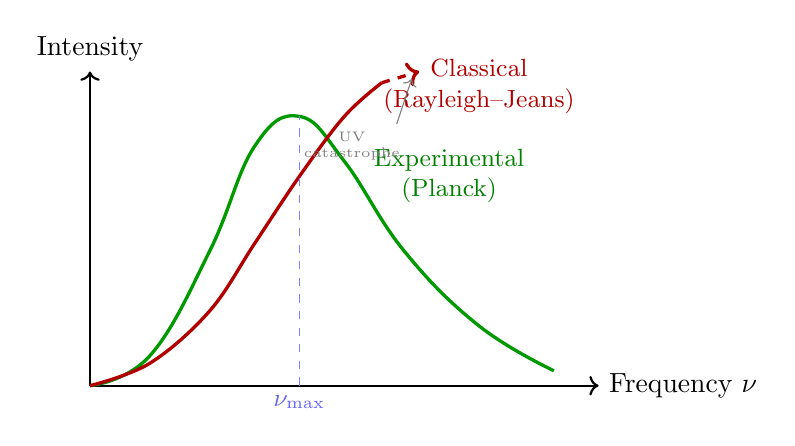
\begin{tikzpicture}[scale=0.95]
  \draw[->,thick] (0,0) -- (6.8,0) node[right] {Frequency $\nu$};
  \draw[->,thick] (0,0) -- (0,4.2) node[above] {Intensity};

  %% Experimental curve (bell shaped)
  \draw[green!60!black, very thick, smooth]
    plot[tension=0.7] coordinates {
      (0,0)(0.8,0.4)(1.6,1.8)(2.2,3.2)(2.8,3.6)
      (3.4,3.0)(4.2,1.8)(5.2,0.8)(6.2,0.2)
    };
  \node[green!50!black, font=\small, align=center] at (4.8,2.8)
    {Experimental\\(Planck)};

  %% Classical curve (diverges)
  \draw[red!70!black, very thick, smooth]
    plot[tension=0.6] coordinates {
      (0,0)(0.8,0.3)(1.6,1.0)(2.2,1.9)
      (2.8,2.8)(3.4,3.6)(3.9,4.05)
    };
  \draw[red!70!black, very thick, dashed, ->]
    (3.9,4.05) -- (4.4,4.2);
  \node[red!70!black, font=\small, align=center] at (5.2,4.0)
    {Classical\\(Rayleigh--Jeans)};

  %% UV catastrophe label
  \draw[->, gray, thin] (4.1,3.5) -- (4.3,4.1);
  \node[gray, font=\tiny, align=center] at (3.5,3.2)
    {UV\\catastrophe};

  %% Peak marker
  \draw[dashed, blue!50] (2.8,0) -- (2.8,3.6);
  \node[below, font=\small, blue!60] at (2.8,0) {$\nu_{\max}$};
\end{tikzpicture}
\end{center}

\begin{center}
\textcolor{cA}{\rule{0.75\textwidth}{0.4pt}}
\end{center}

%% ── Part 3 ────────────────────────────────────────────────────────────
\medskip
\textbf{Part 3: Planck's Quantum Theory as the Solution} \hfill \mk{4}

\medskip
\textbf{(i) Planck's Revolutionary Hypothesis (1900):}

Max Planck resolved the ultraviolet catastrophe by abandoning the classical
assumption of continuous energy. He proposed that oscillating atoms in the
blackbody walls can only emit or absorb energy in discrete packets called
\textbf{quanta}:
\[
  E = nh\nu, \quad n = 0,\,1,\,2,\,3,\ldots
\]
where $h = 6.626\times10^{-34}$ J$\cdot$s is \textbf{Planck's constant}
and $\nu$ is the frequency of oscillation. Energy is therefore
\emph{quantized} --- not continuous.

\medskip
\textbf{(ii) Planck's Radiation Law:}

Using this quantization assumption and Boltzmann statistics, Planck
derived the correct energy density formula:
\[
  \boxed{u(\nu, T)
  = \frac{8\pi h\nu^3}{c^3}
    \cdot \frac{1}{e^{h\nu/k_BT} - 1}}
\]
This single equation perfectly matched \emph{all} experimental blackbody
curves at every temperature --- a complete triumph over classical theory.

\medskip
\textbf{(iii) Why Quantization Eliminates the Catastrophe:}

The key lies in the exponential term $e^{h\nu/k_BT}$. At high frequencies:
\[
  h\nu \gg k_BT
  \quad\Rightarrow\quad
  e^{h\nu/k_BT} \to \infty
  \quad\Rightarrow\quad
  u(\nu,T) \to 0
\]
Physically: at high frequencies, each quantum $h\nu$ is so large that
thermal energy $k_BT$ cannot excite the oscillators --- they are
\emph{frozen out}. This naturally suppresses emission at high frequencies
and prevents the divergence that plagued classical theory.

At low frequencies ($h\nu \ll k_BT$), the exponential reduces to
$e^{h\nu/k_BT} \approx 1 + h\nu/k_BT$, and Planck's law reduces
exactly to the classical Rayleigh--Jeans law --- confirming it is
correct at low frequencies:
\[
  u(\nu,T) \;\xrightarrow{h\nu \ll k_BT}\;
  \frac{8\pi\nu^2}{c^3}\,k_BT
  \quad\checkmark
\]

\begin{center}
\textcolor{cA}{\rule{0.75\textwidth}{0.4pt}}
\end{center}

%% ── Part 4 ────────────────────────────────────────────────────────────
\medskip
\textbf{Part 4: Significance of the Relationship} \hfill \mk{2}

\medskip
\begin{center}
\begin{tabular}{p{0.28\textwidth} p{0.28\textwidth} p{0.28\textwidth}}
\toprule
\textbf{Aspect} & \textbf{Classical Theory} & \textbf{Planck's Quantum Theory} \tabularnewline
\midrule
Nature of energy & Continuous & Discrete quanta $E = h\nu$ \tabularnewline[4pt]
High-frequency behavior & $u \to \infty$ (catastrophe) &
  $u \to 0$ (frozen out) \tabularnewline[4pt]
Low-frequency behavior & Matches experiment & Reduces to Rayleigh--Jeans \tabularnewline[4pt]
Overall spectral curve & Fails completely & Perfect agreement \tabularnewline[4pt]
Physical basis & Equipartition theorem & Boltzmann + quantization \tabularnewline
\bottomrule
\end{tabular}
\end{center}

\medskip
The blackbody problem was the \textbf{birthplace of quantum theory}.
Planck himself called his quantization assumption ``an act of desperation''
--- yet it launched the entire field of modern physics. It directly
inspired Einstein's photon concept (1905), Bohr's atomic model (1913),
and ultimately the full development of quantum mechanics.

\medskip
\begin{center}
\textcolor{cA}{\rule{0.85\textwidth}{0.5pt}}
\end{center}

\medskip
\textbf{Conclusion:} Blackbody radiation was the phenomenon that
classical physics \emph{could not} explain. Planck's revolutionary
insight --- that energy is quantized in units of $h\nu$ --- not only
resolved the ultraviolet catastrophe perfectly but gave birth to quantum
theory itself. The relationship between blackbody radiation and Planck's
quantum theory is therefore not merely historical: it is the \emph{origin}
of our entire modern understanding of the subatomic world.

\end{tcolorbox}

\item Concisely describe the physical significance of $\Psi^2$ for a hydrogen atom. \mk{5}
\yr{CHEM 113 | 2021--22}

\begin{tcolorbox}[enhanced,breakable,ansbox,colback=cA!4,colframe=cA,boxrule=0.8pt,arc=5pt,title={\textbf{Answer}},fonttitle=\bfseries\color{white},colbacktitle=cA]
\textbf{Physical Significance of $\Psi^2$ for a Hydrogen Atom} \hfill \mk{5}

\medskip
\begin{center}
\textcolor{cA}{\rule{0.85\textwidth}{0.5pt}}
\end{center}

\medskip
In quantum mechanics, the wave function $\Psi$ itself has no direct
physical meaning. However, its square, $\Psi^2$ (or more precisely
$|\Psi|^2$ for complex wave functions), carries deep physical
significance:

\medskip
\textbf{(i) Probability Density:}

$|\Psi|^2$ gives the \textbf{probability density} --- the probability
of finding the electron per unit volume at a given point in space.
Specifically, the probability of finding the electron in a small
volume element $dV$ at position $\mathbf{r}$ is:
\[
  P = |\Psi|^2 \, dV
\]
A large value of $|\Psi|^2$ at a point means the electron is
\emph{likely} to be found there; a small value means it is
\emph{unlikely}.

\medskip
\textbf{(ii) Electron Density Cloud:}

For a hydrogen atom, $|\Psi|^2$ describes the \textbf{electron
density cloud} (or probability cloud) around the nucleus. This
replaces the classical idea of a fixed circular orbit (Bohr model)
with a three-dimensional probability distribution. The shape of
this cloud defines what we call an \textbf{atomic orbital}.

\medskip
\textbf{(iii) Normalization Condition:}

Since the electron must exist \emph{somewhere} in space, $|\Psi|^2$
integrated over all space must equal 1:
\[
  \int_{-\infty}^{\infty} |\Psi|^2 \, dV = 1
\]
This ensures $|\Psi|^2$ is a valid probability distribution.

\medskip
\textbf{(iv) Radial Distribution:}

For hydrogen, $|\Psi|^2$ depends on quantum numbers $n$, $l$, $m_l$.
The most probable distance of the electron from the nucleus for the
ground state ($n=1$) corresponds to the Bohr radius:
\[
  a_0 = 0.529 \text{ \AA}
\]
confirming that $|\Psi|^2$ correctly reproduces known atomic
properties.

\medskip
\begin{center}
\textcolor{cA}{\rule{0.85\textwidth}{0.5pt}}
\end{center}

\medskip
\textbf{Conclusion:} $|\Psi|^2$ is the \textbf{probability density}
of finding the electron at a given location. It transforms the
abstract wave function into a physically measurable quantity ---
the spatial distribution of the electron around the nucleus ---
and forms the foundation of the orbital model of the atom.
\end{tcolorbox}

\item Plot the radial probability distribution for a 2s orbital (as a solid line) and a 2p orbital (as a dashed line). For each orbital indicate any radial nodes with an arrow. Compare the shielding experienced by a 2s electron to that of a 2p electron and provide a brief explanation. \mk{10}
\yr{CHEM 113 | 2021--22}

\begin{tcolorbox}[enhanced,breakable,ansbox,colback=cA!4,colframe=cA,boxrule=0.8pt,arc=5pt,title={\textbf{Answer}},fonttitle=\bfseries\color{white},colbacktitle=cA]

\textbf{Radial Probability Distribution — 2s vs 2p:}

\begin{center}
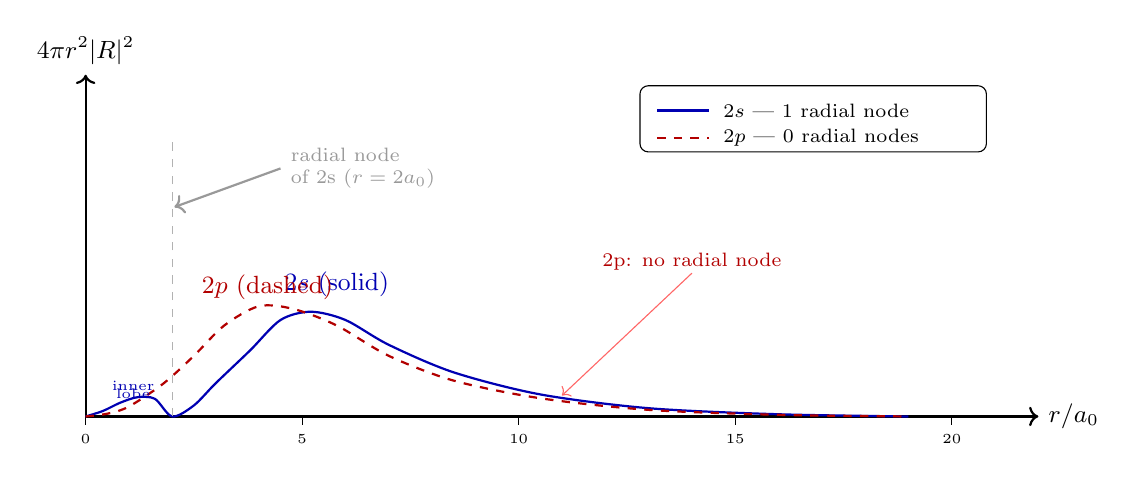
\begin{tikzpicture}[x=0.55cm, y=7cm]

  %% axes
  \draw[->, thick] (0,0) -- (22,0)
    node[right, font=\small] {$r/a_0$};
  \draw[->, thick] (0,0) -- (0,0.62)
    node[above, font=\small] {$4\pi r^2|R|^2$};

  %% x-axis ticks
  \foreach \x in {0,5,10,15,20}{
    \draw (\x,0) -- (\x,-0.015)
      node[below, font=\tiny] {\x};
  }

  %% ---- 2s (solid line) ----
  \draw[blue!70!black, thick]
    plot[smooth, tension=0.5] coordinates {
      (0,0)(0.4,0.01)(0.8,0.025)(1.2,0.035)(1.6,0.032)
      (2.0,0.0)
      (2.5,0.02)(3.0,0.06)(3.8,0.12)(4.5,0.175)
      (5.2,0.19)(6.0,0.175)(7.0,0.13)(8.5,0.08)
      (10.5,0.04)(13,0.015)(16,0.004)(19,0)
    };

  %% ---- 2p (dashed line) ----
  \draw[red!70!black, thick, dashed]
    plot[smooth, tension=0.5] coordinates {
      (0,0)(0.5,0.005)(1.0,0.018)(1.8,0.06)(2.5,0.11)
      (3.2,0.165)(4.0,0.20)(4.8,0.195)(5.8,0.165)(7.0,0.11)
      (8.5,0.065)(10.5,0.033)(13,0.012)(16,0.003)(19,0)
    };

  %% ---- inner lobe label for 2s ----
  \node[blue!70!black, font=\tiny] at (1.1,0.055) {inner};
  \node[blue!70!black, font=\tiny] at (1.1,0.042) {lobe};

  %% ---- radial node arrow for 2s at r=2a0 ----
  \draw[dashed, gray!60, thin] (2.0,0) -- (2.0,0.50);
  \draw[->, thick, gray!80] (4.5,0.45)
    node[right, font=\scriptsize, gray!80,
         align=left] {radial node\\of 2s ($r=2a_0$)}
    -- (2.05,0.38);

  %% ---- node label for 2p: no radial node ----
  \node[red!70!black, font=\scriptsize] at (14,0.28)
    {2p: no radial node};
  \draw[->, red!60] (14,0.26) -- (11,0.038);

  %% ---- orbital labels ----
  \node[blue!70!black, font=\small, align=center] at (5.8,0.24)
    {$2s$ (solid)};
  \node[red!70!black,  font=\small, align=center] at (4.2,0.235)
    {$2p$ (dashed)};

  %% ---- legend ----
  \draw[rounded corners=3pt] (12.8,0.48) rectangle (20.8,0.60);
  \draw[blue!70!black, thick]        (13.2,0.555) -- (14.4,0.555);
  \node[right, font=\scriptsize] at  (14.5,0.555) {$2s$ — 1 radial node};
  \draw[red!70!black,  thick, dashed](13.2,0.505) -- (14.4,0.505);
  \node[right, font=\scriptsize] at  (14.5,0.505) {$2p$ — 0 radial nodes};

\end{tikzpicture}
\end{center}

\bigskip
\textbf{Comparison of Shielding — 2s vs 2p:}

\textbf{Shielding} (or screening) refers to the reduction in the effective nuclear
charge $Z_{\text{eff}}$ experienced by an electron, caused by the repulsion from
inner-shell electrons that partially cancel the nuclear attraction:
\[
  Z_{\text{eff}} = Z - \sigma
\]
where $Z$ is the atomic number and $\sigma$ is the shielding constant.

\begin{enumerate}

  \item \textbf{2s electron — less shielded (higher $Z_{\text{eff}}$):}\\
  The 2s radial wavefunction:
  \[
    R_{20}(r) \propto \left(2 - \frac{r}{a_0}\right)e^{-r/2a_0}
  \]
  has a \textbf{small inner lobe} (before the radial node at $r = 2a_0$) that gives
  the 2s electron significant probability of \textbf{penetrating inside} the 1s
  core electrons. In this inner region, the electron is nearly unshielded and
  experiences the full nuclear charge $Z$. This penetration \textbf{reduces} the
  effective shielding:
  \[
    \sigma_{2s} < \sigma_{2p} \quad \Longrightarrow \quad Z_{\text{eff}}(2s) > Z_{\text{eff}}(2p)
  \]

  \item \textbf{2p electron — more shielded (lower $Z_{\text{eff}}$):}\\
  The 2p radial wavefunction:
  \[
    R_{21}(r) \propto \frac{r}{a_0}\,e^{-r/2a_0}
  \]
  vanishes at $r = 0$ due to the angular momentum barrier ($l = 1$). The 2p
  electron has \textbf{no inner lobe} and \textbf{cannot penetrate} the 1s core.
  It therefore spends all its time \textit{outside} the core electrons, which
  fully shield it from the nucleus, resulting in a lower $Z_{\text{eff}}$.

  \item \textbf{Consequence on energy:}\\
  Since the 2s electron experiences a higher $Z_{\text{eff}}$, it is more
  strongly attracted to the nucleus and has a \textbf{lower (more negative) energy}
  than the 2p electron:
  \[
    E_{2s} < E_{2p}
  \]
  This is why, in multi-electron atoms, the 2s subshell \textbf{fills before} the
  2p subshell (aufbau principle), and the 2s--2p energy gap increases across
  Period 2.

\end{enumerate}

\bigskip
\textbf{Summary:}
\begin{center}
\begin{tabular}{p{2cm} p{3cm} p{2.5cm} p{3cm}}
\toprule
\textbf{Orbital} & \textbf{Penetration} & \textbf{Shielding $\sigma$} & \textbf{$Z_{\text{eff}}$} \\
\midrule
$2s$ & High (inner lobe) & Lower & Higher — closer to nucleus \\[3pt]
$2p$ & None (angular barrier) & Higher & Lower — farther from nucleus \\
\bottomrule
\end{tabular}
\end{center}

\textbf{Conclusion:} The \textbf{penetration} of the 2s orbital through the inner
electron core, arising from its inner probability lobe, causes it to experience
\textbf{less shielding} and a \textbf{higher effective nuclear charge} compared to
the 2p orbital. This makes the 2s electron more tightly bound and lower in energy.

\end{tcolorbox}

\item Consider a Ca$^{19+}$ ion with its electron in the 5th excited state. (i) Calculate the longest wavelength of light that could be emitted when the Ca$^{19+}$ electron transitions to a lower energy state. (ii) Suppose the same transition as in part (i) took place in a hydrogen atom. Would the wavelength of emission be longer than, shorter than, or the same as your answer? \mk{10}
\yr{CHEM 113 | 2021--22}

\begin{tcolorbox}[enhanced,breakable,ansbox,colback=cA!4,colframe=cA,boxrule=0.8pt,arc=5pt,title={\textbf{Answer}},fonttitle=\bfseries\color{white},colbacktitle=cA]
\textbf{Given:}
\begin{itemize}
  \item Ca$^{19+}$ is a \textbf{hydrogenic ion} (one electron), atomic number $Z = 20$
  \item 5th excited state $\Rightarrow$ $n = 1 + 5 = 6$
  \item Energy formula for a hydrogenic ion:
  \[
    E_n = -\frac{Z^2 \times 13.6}{n^2} \text{ eV}
  \]
\end{itemize}

\bigskip
\textbf{(i) Longest wavelength of emitted light:}

Longest wavelength $\Rightarrow$ lowest energy $\Rightarrow$ smallest $\Delta E$
$\Rightarrow$ transition to the \textbf{nearest lower level}:
$n = 6 \rightarrow n = 5$

\textbf{Calculate $E_6$ and $E_5$:}
\[
  E_6 = -\frac{(20)^2 \times 13.6}{6^2}
      = -\frac{400 \times 13.6}{36}
      = -\frac{5440}{36}
      = -151.11 \text{ eV}
\]
\[
  E_5 = -\frac{(20)^2 \times 13.6}{5^2}
      = -\frac{400 \times 13.6}{25}
      = -\frac{5440}{25}
      = -217.60 \text{ eV}
\]

\textbf{Energy of emitted photon:}
\[
  \Delta E = E_6 - E_5 = -151.11 - (-217.60) = 66.49 \text{ eV}
\]

Converting to Joules:
\[
  \Delta E = 66.49 \times 1.602 \times 10^{-19}
           = 1.065 \times 10^{-17} \text{ J}
\]

\textbf{Wavelength:}
\[
  \lambda = \frac{hc}{\Delta E}
          = \frac{(6.626 \times 10^{-34})(3.0 \times 10^8)}{1.065 \times 10^{-17}}
\]
\[
  \boxed{\lambda = 1.867 \times 10^{-8} \text{ m} = 18.67 \text{ nm}}
\]
This falls in the \textbf{extreme UV region} of the electromagnetic spectrum.

\bigskip
\textbf{(ii) Same transition ($n=6 \rightarrow n=5$) in hydrogen ($Z=1$):}

\[
  \Delta E_H = 13.6\left(\frac{1}{5^2} - \frac{1}{6^2}\right)
             = 13.6\left(\frac{1}{25} - \frac{1}{36}\right)
             = 13.6 \times \frac{36 - 25}{25 \times 36}
             = 13.6 \times \frac{11}{900}
             = 0.1662 \text{ eV}
\]

\[
  \Delta E_H = 0.1662 \times 1.602 \times 10^{-19}
             = 2.663 \times 10^{-20} \text{ J}
\]

\[
  \lambda_H = \frac{hc}{\Delta E_H}
            = \frac{(6.626\times10^{-34})(3.0\times10^8)}{2.663\times10^{-20}}
            = 7.468 \times 10^{-6} \text{ m}
\]
\[
  \boxed{\lambda_H = 7{,}468 \text{ nm} \approx 7.47\ \mu\text{m}}
\]
This falls in the \textbf{infrared region}.

\bigskip
\textbf{Comparison:}
\begin{center}
\begin{tabular}{p{3.5cm} p{3cm} p{3.2cm} p{2.5cm}}
\toprule
\textbf{System} & \textbf{$\Delta E$} & \textbf{$\lambda$} & \textbf{Region} \\
\midrule
Ca$^{19+}$ ($Z=20$) & $66.49$ eV  & $18.67$ nm      & Extreme UV \\[3pt]
H ($Z=1$)           & $0.166$ eV  & $7{,}468$ nm    & Infrared \\
\bottomrule
\end{tabular}
\end{center}

The hydrogen wavelength is \textbf{much longer} than that of Ca$^{19+}$.

\textbf{Reason:} For the same transition, energy scales as $Z^2$:
\[
  \Delta E \propto Z^2 \qquad \Longrightarrow \qquad \lambda \propto \frac{1}{Z^2}
\]
Since $Z = 20$ for Ca$^{19+}$, the transition energy is $Z^2 = 400$ times
larger than for hydrogen, making the wavelength 400 times \textit{shorter}.
Verification:
\[
  \frac{\lambda_H}{\lambda_{\text{Ca}^{19+}}}
  = \frac{7468}{18.67} \approx 400 = Z^2 \quad \checkmark
\]

\textbf{Conclusion:} For the same $n = 6 \rightarrow 5$ transition, hydrogen
emits at $7{,}468$ nm (infrared), which is \textbf{far longer} than the
$18.67$ nm (extreme UV) emitted by Ca$^{19+}$. The $Z^2$ dependence of
transition energies in hydrogenic systems means that higher nuclear charge
produces far more energetic — and therefore far shorter wavelength —
emissions.
\end{tcolorbox}

\item Explain why elements produce their own characteristic colors when they emit photons. How is the concept of electron density used to describe the motions and energies of submicroscopic particles in the quantum mechanical treatment of an atom? \mk{15}
\yr{CHEM 113 | 2020--21 (Jan 21)}

\begin{tcolorbox}[enhanced,breakable,ansbox,colback=cA!4,colframe=cA,boxrule=0.8pt,arc=5pt,title={\textbf{Answer}},fonttitle=\bfseries\color{white},colbacktitle=cA]

\textbf{Part 1: Characteristic Colors from Photon Emission} \hfill \mk{7}

\medskip
Each element emits photons of specific wavelengths (colors) because its electrons
occupy \emph{discrete, quantized energy levels} unique to that element.

When an electron transitions from a higher energy level $E_2$ to a lower level $E_1$,
it emits a photon whose energy equals the difference:
\[
  \Delta E = E_2 - E_1 = h\nu = \frac{hc}{\lambda}
\]
where $h$ is Planck's constant, $\nu$ is the photon frequency, and $\lambda$ is its
wavelength. Since $\lambda$ determines color, and each element has a \emph{unique}
set of energy levels, each element produces its own unique spectrum of colors ---
its spectral ``fingerprint.''

\medskip
\textbf{Example --- Hydrogen:} The Balmer series gives visible lines (e.g.\
$n=3\to2$ gives red at 656 nm; $n=4\to2$ gives blue-green at 486 nm).

\medskip
\textbf{Part 2: Electron Density in Quantum Mechanical Treatment} \hfill \mk{8}

\medskip
In classical mechanics, electron motion is described by a definite trajectory.
Quantum mechanics replaces this with the \textbf{wave function} $\psi$, obtained by
solving the Schr\"{o}dinger equation:
\[
  \hat{H}\,\psi = E\,\psi
\]

\medskip
\textbf{(i) Physical meaning of $|\psi|^2$:}
The square of the wave function, $|\psi|^2$, gives the \emph{probability density}
--- i.e., the probability of finding the electron per unit volume at a given point
in space. This is called the \textbf{electron density}.

\medskip
\textbf{(ii) Describing Motion:}
Instead of saying ``the electron moves in a circular orbit'' (Bohr), quantum
mechanics states that the electron exists as a \emph{probability cloud} or
\emph{electron density cloud} around the nucleus. Regions of high $|\psi|^2$ are
where the electron is most likely to be found.

\medskip
\textbf{(iii) Describing Energy:}
Each wave function $\psi_{n,l,m_l}$ corresponds to a definite, quantized energy
$E_n$. For hydrogen:
\[
  E_n = -\frac{13.6 \text{ eV}}{n^2}, \quad n = 1, 2, 3, \ldots
\]
Higher $n$ means a more diffuse electron cloud (larger orbital) and higher
(less negative) energy.

\medskip
\textbf{(iv) Heisenberg Uncertainty \& Electron Density:}
Because we cannot simultaneously know the exact position and momentum of an
electron (Heisenberg's Uncertainty Principle: $\Delta x \cdot \Delta p \geq h/4\pi$),
electron density is the most physically meaningful description possible ---
it tells us \emph{where} the electron is likely to be, not a fixed path.

\end{tcolorbox}

\item What role did Einstein's explanation of the photoelectric effect play in the development of the particle-wave interpretation of the nature of electromagnetic radiation? Does a baseball in motion possess wave properties? If so, why can we not determine its wave properties? \mk{20}
\yr{CHEM 113 | 2020--21 (Jan 21)}

\begin{tcolorbox}[enhanced,breakable,ansbox,colback=cA!4,colframe=cA,boxrule=0.8pt,arc=5pt,title={\textbf{Answer}},fonttitle=\bfseries\color{white},colbacktitle=cA]

\textbf{Part 1: Einstein's Photoelectric Effect \& Wave--Particle Duality of Light}
\hfill \mk{12}

\medskip
\textbf{(i) Background --- The Classical Wave Picture \& Its Failure:}

Before Einstein, light was understood purely as an electromagnetic \emph{wave}
(Maxwell, 1865). The classical wave theory predicted that:
\begin{itemize}[leftmargin=1.5em, itemsep=2pt]
  \item Any frequency of light, given enough intensity, should eject electrons.
  \item Higher intensity $\Rightarrow$ higher kinetic energy of ejected electrons.
  \item There should be a measurable time delay before electrons are emitted.
\end{itemize}
Experiments showed \emph{none} of these predictions were correct --- classical
wave theory completely failed to explain the photoelectric effect.

\medskip
\textbf{(ii) Einstein's Explanation (1905):}

Einstein proposed that light is not a continuous wave but is made of discrete
energy packets called \textbf{photons}. The energy of each photon depends only
on its frequency:
\[
  E = h\nu
\]
where $h = 6.626 \times 10^{-34}$ J$\cdot$s is Planck's constant and $\nu$ is
the frequency of light.

A single photon interacts with a single electron. The electron is ejected only
if the photon energy $h\nu$ exceeds the \textbf{work function} $\phi$ (the
minimum energy needed to remove the electron from the metal surface):
\[
  h\nu = \phi + \frac{1}{2}mv^2_{\max}
\]
\[
  \Rightarrow\quad \frac{1}{2}mv^2_{\max} = h\nu - h\nu_0 = h(\nu - \nu_0)
\]
where $\nu_0 = \phi/h$ is the \textbf{threshold frequency}. Below $\nu_0$,
no electrons are emitted regardless of intensity.

\medskip
\textbf{(iii) Key Experimental Facts Explained:}

\begin{center}
\begin{tabular}{p{0.42\textwidth} p{0.48\textwidth}}
\toprule
\textbf{Observation} & \textbf{Einstein's Explanation} \\
\midrule
No emission below threshold frequency $\nu_0$ &
  Photon energy $h\nu < \phi$; not enough to free electron \\[4pt]
KE of electrons depends on $\nu$, not intensity &
  Each electron absorbs exactly one photon; KE $= h(\nu-\nu_0)$ \\[4pt]
Emission is instantaneous &
  One photon $\to$ one electron; no energy accumulation needed \\[4pt]
More intensity $\Rightarrow$ more electrons, not faster ones &
  More photons $\Rightarrow$ more collisions, but each photon carries same $h\nu$ \\
\bottomrule
\end{tabular}
\end{center}

\medskip
\textbf{(iv) Role in Wave--Particle Duality of Electromagnetic Radiation:}

Einstein's work created a profound dilemma:
\begin{itemize}[leftmargin=1.5em, itemsep=3pt]
  \item Young's double-slit experiment (1801) and Maxwell's equations
        \emph{proved} light is a wave --- it diffracts and interferes.
  \item Einstein's photoelectric effect \emph{proved} light behaves as a
        particle (photon) --- it collides with electrons one-to-one.
\end{itemize}
Neither picture alone is complete. Light exhibits \textbf{wave--particle duality}:
\[
  \text{Wave nature:}\;\lambda,\;\nu,\;\text{diffraction, interference}
  \qquad
  \text{Particle nature:}\; E = h\nu,\; p = \frac{h}{\lambda}
\]
This became the cornerstone of quantum mechanics and directly inspired
de~Broglie (1924) to ask: \emph{if waves can behave as particles, can particles
behave as waves?}

\bigskip
\textbf{Part 2: Does a Baseball Possess Wave Properties?} \hfill \mk{8}

\medskip
\textbf{(i) de~Broglie's Hypothesis:}

In 1924, de~Broglie proposed that \emph{all} matter --- not just light ---
has an associated wavelength:
\[
  \lambda = \frac{h}{mv} = \frac{h}{p}
\]
where $m$ is the mass, $v$ is the velocity, and $p = mv$ is the momentum
of the object. This applies to \emph{every} moving object, including a baseball.

\medskip
\textbf{(ii) Calculation for a Baseball:}

Consider a baseball of mass $m = 0.145$ kg moving at $v = 40$ m/s:
\[
  \lambda = \frac{h}{mv}
  = \frac{6.626 \times 10^{-34}}{0.145 \times 40}
  = \frac{6.626 \times 10^{-34}}{5.8}
  \approx 1.14 \times 10^{-34} \text{ m}
\]

\medskip
\textbf{(iii) Why We Cannot Observe the Baseball's Wave Properties:}

\begin{itemize}[leftmargin=1.5em, itemsep=4pt]
  \item The de~Broglie wavelength of the baseball,
        $\lambda \approx 10^{-34}$ m, is \emph{incomprehensibly} smaller than
        anything measurable. For comparison:
        \[
          \text{diameter of a proton} \approx 10^{-15}\text{ m}
          \quad\gg\quad \lambda_{\text{baseball}} \approx 10^{-34}\text{ m}
        \]
  \item Wave properties such as diffraction and interference are only observable
        when the wavelength is \emph{comparable} to the size of the obstacle or
        slit. No physical apparatus can come close to resolving $10^{-34}$ m.
  \item For \emph{subatomic} particles like electrons ($m \approx 9.1\times10^{-31}$
        kg), $\lambda$ falls in the \AA ngstr\"{o}m range ($\sim 10^{-10}$ m),
        comparable to atomic spacings --- hence electrons \emph{do} show
        measurable diffraction (Davisson--Germer experiment, 1927).
  \item The Heisenberg Uncertainty Principle also tells us that for a
        macroscopic object the uncertainty in momentum required to detect
        wave behavior would be physically meaningless:
        \[
          \Delta x \cdot \Delta p \;\geq\; \frac{h}{4\pi}
        \]
        For a baseball, $\Delta p$ is negligibly small compared to $mv$,
        so quantum effects are entirely undetectable.
\end{itemize}

\medskip
\textbf{Conclusion:}

Yes, a baseball \emph{does} possess wave properties according to de~Broglie's
relation $\lambda = h/mv$. However, because its mass is enormous compared to
subatomic particles, its wavelength is so vanishingly small
($\sim 10^{-34}$ m) that no experiment can detect it. Wave--particle duality
is a universal property of matter, but it is only \emph{observable} at the
quantum (subatomic) scale where $\lambda$ becomes comparable to atomic dimensions.

\end{tcolorbox}

\item Show the radial distribution function for hydrogenic 1s, 2s and 2p orbitals with nodes. Why does 2s give the electron a greater probability of close approach to the nucleus compared to 2p orbital? \mk{10}
\yr{CHEM 113 | 2020--21}

\begin{tcolorbox}[enhanced,breakable,ansbox,colback=cA!4,colframe=cA,boxrule=0.8pt,arc=5pt,title={\textbf{Answer}},fonttitle=\bfseries\color{white},colbacktitle=cA]
The \textbf{radial distribution function (RDF)} gives the probability of finding an electron
in a thin spherical shell of radius $r$:
\[
  P(r) = 4\pi r^2 [R_{nl}(r)]^2
\]

\bigskip
\textbf{RDF Plots for 1s, 2s, and 2p:}

\begin{center}
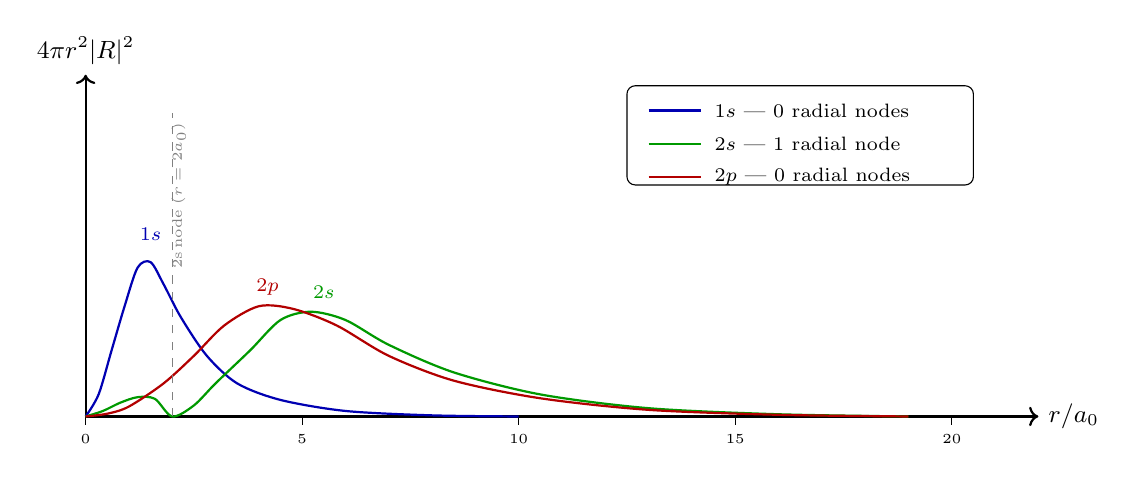
\begin{tikzpicture}[x=0.55cm, y=7cm]

  %% axes
  \draw[->, thick] (0,0) -- (22,0) node[right, font=\small] {$r/a_0$};
  \draw[->, thick] (0,0) -- (0,0.62) node[above, font=\small] {$4\pi r^2|R|^2$};

  %% x-axis ticks
  \foreach \x in {0,5,10,15,20}{
    \draw (\x,0) -- (\x,-0.015) node[below, font=\tiny] {\x};
  }

  %% 1s
  \draw[blue!70!black, thick]
    plot[smooth, tension=0.5] coordinates {
      (0,0)(0.3,0.04)(0.6,0.12)(0.9,0.20)(1.2,0.27)(1.5,0.28)
      (1.8,0.24)(2.2,0.18)(2.8,0.11)(3.5,0.06)(4.5,0.03)
      (6,0.01)(8,0.002)(10,0)
    };
  \node[blue!70!black, font=\scriptsize] at (1.5,0.33) {$1s$};

  %% 2s
  \draw[green!60!black, thick]
    plot[smooth, tension=0.5] coordinates {
      (0,0)(0.4,0.01)(0.8,0.025)(1.2,0.035)(1.6,0.032)
      (2.0,0.0)(2.5,0.02)(3.0,0.06)(3.8,0.12)(4.5,0.175)
      (5.2,0.19)(6.0,0.175)(7.0,0.13)(8.5,0.08)(10.5,0.04)
      (13,0.015)(16,0.004)(19,0)
    };
  \node[green!60!black, font=\scriptsize] at (5.5,0.225) {$2s$};

  %% 2p
  \draw[red!70!black, thick]
    plot[smooth, tension=0.5] coordinates {
      (0,0)(0.5,0.005)(1.0,0.018)(1.8,0.06)(2.5,0.11)
      (3.2,0.165)(4.0,0.20)(4.8,0.195)(5.8,0.165)(7.0,0.11)
      (8.5,0.065)(10.5,0.033)(13,0.012)(16,0.003)(19,0)
    };
  \node[red!70!black, font=\scriptsize] at (4.2,0.235) {$2p$};

  %% node marker for 2s at r=2
  \draw[dashed, gray, thin] (2.0,0) -- (2.0,0.55);
  \node[gray, font=\tiny, rotate=90] at (2.15,0.40) {2s\,node\;($r=2a_0$)};

  %% legend
  \draw[rounded corners=3pt] (12.5,0.42) rectangle (20.5,0.60);
  \draw[blue!70!black,  thick] (13.0,0.555) -- (14.2,0.555);
  \node[right, font=\scriptsize] at (14.3,0.555) {$1s$ — 0 radial nodes};
  \draw[green!60!black, thick] (13.0,0.495) -- (14.2,0.495);
  \node[right, font=\scriptsize] at (14.3,0.495) {$2s$ — 1 radial node};
  \draw[red!70!black,   thick] (13.0,0.435) -- (14.2,0.435);
  \node[right, font=\scriptsize] at (14.3,0.435) {$2p$ — 0 radial nodes};

\end{tikzpicture}
\end{center}

\bigskip
\textbf{Nodal Structure:}
\begin{center}
\begin{tabular}{p{1.5cm} p{2.8cm} p{2.8cm} p{2.8cm}}
\toprule
\textbf{Orbital} & \textbf{Radial nodes} $(n-l-1)$ & \textbf{Angular nodes} $(l)$ & \textbf{Peak position} \\
\midrule
$1s$ & 0 & 0 & $r = a_0$ \\[3pt]
$2s$ & 1\ \ (at $r = 2a_0$) & 0 & $r \approx 5a_0$ (major) \\[3pt]
$2p$ & 0 & 1\ \ (nodal plane) & $r \approx 4a_0$ \\
\bottomrule
\end{tabular}
\end{center}

\bigskip
\textbf{Why 2s gives greater probability of close approach than 2p:}

\begin{enumerate}
  \item \textbf{Penetration via inner lobe:}
  The radial wavefunction of the 2s orbital is:
  \[
    R_{20}(r) = \frac{1}{2\sqrt{2}}\!\left(\frac{1}{a_0}\right)^{3/2}\!\left(2 - \frac{r}{a_0}\right)e^{-r/2a_0}
  \]
  The factor $\left(2 - r/a_0\right)$ does not vanish at $r = 0$, so the 2s RDF has a
  \textbf{small but nonzero inner peak} between $r = 0$ and the node at $r = 2a_0$.
  This inner lobe represents a real probability of finding the 2s electron
  very close to the nucleus — even inside the 1s shell.

  \item \textbf{Angular momentum barrier for 2p:}
  The radial wavefunction of the 2p orbital contains the factor $r/a_0$:
  \[
    R_{21}(r) = \frac{1}{2\sqrt{6}}\!\left(\frac{1}{a_0}\right)^{3/2}\frac{r}{a_0}\,e^{-r/2a_0}
  \]
  This factor forces $R_{21}(0) = 0$, meaning the 2p RDF is \textbf{strictly zero at the
  nucleus}. Physically, the angular momentum ($l = 1$) creates a centrifugal
  barrier that repels the electron away from the nucleus — there is no inner peak
  and no penetration.

  \item \textbf{Consequence — effective nuclear charge:}
  Because the 2s electron penetrates closer to the nucleus, it experiences
  less shielding from inner electrons and sees a higher effective nuclear charge:
  \[
    Z_{\text{eff}}(2s) > Z_{\text{eff}}(2p)
  \]
  This makes the 2s electron \textbf{more tightly bound} and lower in energy than the
  2p electron — which is why $2s$ fills before $2p$ in the aufbau principle.
\end{enumerate}

\bigskip
\textbf{Conclusion:} The presence of a \textbf{radial node} in the 2s orbital creates an
inner probability lobe (penetration), giving the 2s electron significant access to
the nuclear region. The 2p electron, excluded by its angular momentum barrier
($l=1$), has no such inner peak — making 2s electrons closer to and more
strongly bound by the nucleus than 2p electrons.
\end{tcolorbox}

\item In making a transition from an orbital with a principal quantum number of 4 to an orbital with a principal quantum number of 7, does the electron of a hydrogen atom emit or absorb a photon of energy? What would be the energy of the photon? To what region of the electromagnetic spectrum does this energy correspond? \mk{10}
\yr{CHEM 113 | 2020--21}

\begin{tcolorbox}[enhanced,breakable,ansbox,colback=cA!4,colframe=cA,boxrule=0.8pt,arc=5pt,title={\textbf{Answer}},fonttitle=\bfseries\color{white},colbacktitle=cA]
\textbf{Given:}
\begin{itemize}
  \item Hydrogen atom: $Z = 1$
  \item Initial state: $n_i = 4$
  \item Final state: $n_f = 7$
  \item Energy of hydrogen atom:
  \[
    E_n = -\frac{13.6}{n^2} \text{ eV}
  \]
\end{itemize}

\bigskip
\textbf{(i) Emission or Absorption?}

The electron transitions from $n = 4$ \textbf{to} $n = 7$, i.e.\ from a
\textbf{lower} to a \textbf{higher} energy level. Moving away from the nucleus
requires energy input. Therefore, the electron \textbf{absorbs} a photon.

\[
  n_i = 4 \;\longrightarrow\; n_f = 7 \qquad
  \text{(upward transition} \Rightarrow \textbf{absorption)}
\]

\bigskip
\textbf{(ii) Energy of the photon:}

\textbf{Calculate $E_4$ and $E_7$:}
\[
  E_4 = -\frac{13.6}{4^2} = -\frac{13.6}{16} = -0.850 \text{ eV}
\]
\[
  E_7 = -\frac{13.6}{7^2} = -\frac{13.6}{49} = -0.2776 \text{ eV}
\]

\textbf{Energy of absorbed photon:}
\[
  \Delta E = E_7 - E_4 = -0.2776 - (-0.850) = +0.5724 \text{ eV}
\]
The positive sign confirms \textbf{absorption}.

Converting to Joules:
\[
  \Delta E = 0.5724 \times 1.602 \times 10^{-19}
           = 9.17 \times 10^{-20} \text{ J}
\]

\[
  \boxed{\Delta E = +0.5724 \text{ eV} = 9.17 \times 10^{-20} \text{ J}}
\]

\bigskip
\textbf{(iii) Wavelength and region of electromagnetic spectrum:}

\[
  \lambda = \frac{hc}{\Delta E}
          = \frac{(6.626 \times 10^{-34})(3.0 \times 10^8)}{9.17 \times 10^{-20}}
\]
\[
  \lambda = \frac{1.988 \times 10^{-25}}{9.17 \times 10^{-20}}
          = 2.168 \times 10^{-6} \text{ m}
\]
\[
  \boxed{\lambda = 2168 \text{ nm} \approx 2.17\ \mu\text{m}}
\]

\bigskip
\textbf{Electromagnetic Spectrum Region:}

\begin{center}
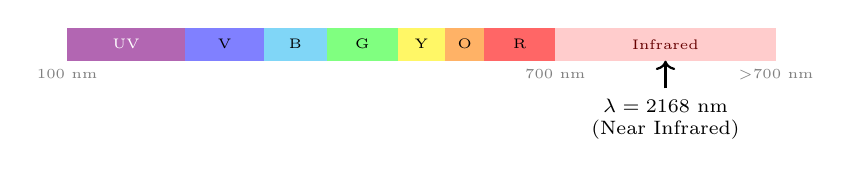
\begin{tikzpicture}[x=1.0cm, y=0.7cm]

  %% spectrum bar
  \fill[violet!60]  (0,0)   rectangle (1.5, 0.6);
  \fill[blue!50]    (1.5,0) rectangle (2.5, 0.6);
  \fill[cyan!50]    (2.5,0) rectangle (3.3, 0.6);
  \fill[green!50]   (3.3,0) rectangle (4.2, 0.6);
  \fill[yellow!60]  (4.2,0) rectangle (4.8, 0.6);
  \fill[orange!60]  (4.8,0) rectangle (5.3, 0.6);
  \fill[red!60]     (5.3,0) rectangle (6.2, 0.6);
  \fill[red!20]     (6.2,0) rectangle (9.0, 0.6);

  %% labels inside bar
  \node[font=\tiny, white]         at (0.75, 0.30) {UV};
  \node[font=\tiny]                at (2.00, 0.30) {V};
  \node[font=\tiny]                at (2.90, 0.30) {B};
  \node[font=\tiny]                at (3.75, 0.30) {G};
  \node[font=\tiny]                at (4.50, 0.30) {Y};
  \node[font=\tiny]                at (5.05, 0.30) {O};
  \node[font=\tiny]                at (5.75, 0.30) {R};
  \node[font=\tiny, red!40!black]  at (7.60, 0.30) {Infrared};

  %% arrow pointing to IR region
  \draw[->, thick, black] (7.60, -0.5)
    node[below, font=\scriptsize, align=center]
      {$\lambda = 2168$ nm\\(Near Infrared)}
    -- (7.60, 0.0);

  %% wavelength axis
  \node[font=\tiny, gray] at (0.0,  -0.25) {100 nm};
  \node[font=\tiny, gray] at (6.2,  -0.25) {700 nm};
  \node[font=\tiny, gray] at (9.0,  -0.25) {$>$700 nm};

\end{tikzpicture}
\end{center}

Since $\lambda = 2168$ nm lies well beyond the visible red limit of
$\sim$700 nm, this photon belongs to the \textbf{near-infrared (NIR) region}
of the electromagnetic spectrum.

\bigskip
\textbf{Summary:}
\begin{center}
\begin{tabular}{p{4.5cm} p{6cm}}
\toprule
\textbf{Quantity} & \textbf{Value} \\
\midrule
Transition          & $n=4 \rightarrow n=7$ (absorption) \\[3pt]
$\Delta E$          & $+0.5724$ eV $= 9.17\times10^{-20}$ J \\[3pt]
$\lambda$           & $2168$ nm $= 2.17\ \mu$m \\[3pt]
Spectral region     & Near-infrared (NIR) \\[3pt]
Spectral series     & Brackett series ($n_f = 4$) \\
\bottomrule
\end{tabular}
\end{center}

\textbf{Conclusion:} Since the transition is from a lower ($n=4$) to a higher
($n=7$) energy level, the electron \textbf{absorbs} a photon of energy
$0.5724$ eV. The corresponding wavelength of $2168$ nm places this
absorption in the \textbf{near-infrared} region, specifically within the
\textbf{Brackett series} of the hydrogen spectrum.
\end{tcolorbox}

\item Account for the large decrease in electron affinity between Li and Be despite the increase in nuclear charge? \mk{5}
\yr{CHEM 113 | 2020--21}

\begin{tcolorbox}[enhanced,breakable,ansbox,colback=cA!4,colframe=cA,boxrule=0.8pt,arc=5pt,title={\textbf{Answer}},fonttitle=\bfseries\color{white},colbacktitle=cA]
\textbf{Electron Affinities:}
\[
  \text{Li}: -59.6\text{ kJ/mol} \qquad \text{Be}: \approx +18\text{ kJ/mol}
\]
Be has a \textbf{positive} (unfavourable) electron affinity despite having
a higher nuclear charge ($Z = 4$) than Li ($Z = 3$). This seems
contradictory but is explained by their electron configurations:

\bigskip
\textbf{Electron Configurations:}
\[
  \text{Li}: 1s^2\,2s^1 \qquad \text{Be}: 1s^2\,2s^2
\]

\textbf{Li} adding an electron:
\[
  \text{Li} + e^- \;\rightarrow\; \text{Li}^-: 1s^2\,2s^2
  \qquad \Delta E = -59.6\text{ kJ/mol} \quad \text{(favourable)}
\]
The incoming electron enters the \textbf{vacant} $2s$ orbital —
no extra repulsion, moderate $Z_{\text{eff}}$, stabilisation occurs.

\textbf{Be} adding an electron:
\[
  \text{Be} + e^- \;\rightarrow\; \text{Be}^-: 1s^2\,2s^2\,2p^1
  \qquad \Delta E \approx +18\text{ kJ/mol} \quad \text{(unfavourable)}
\]
The $2s$ subshell is \textbf{completely full} in Be. The incoming
electron must enter the \textbf{higher energy} $2p$ orbital.

\bigskip
\textbf{Three reasons for the large decrease:}

\begin{enumerate}

  \item \textbf{Subshell energy penalty:}\\
  The $2p$ orbital is \textbf{higher in energy} than $2s$ due to
  poorer penetration and greater shielding:
  \[
    E_{2p} > E_{2s}
  \]
  Placing the extra electron in $2p$ requires overcoming this
  energy gap — making the process \textit{endothermic}.

  \item \textbf{Increased shielding in $2p$:}\\
  The added electron in the $2p$ orbital is \textbf{more shielded}
  by the filled $2s^2$ electrons than Li's added electron was.
  This reduces $Z_{\text{eff}}$ felt by the incoming electron in Be,
  despite the higher nuclear charge:
  \[
    Z_{\text{eff}}(\text{Be, }2p) < Z_{\text{eff}}(\text{Li, }2s)
  \]

  \item \textbf{Stability of filled subshell:}\\
  Be has a \textbf{completely filled} $2s^2$ subshell, which
  confers extra stability (exchange energy). Disrupting this
  closed-subshell configuration by forcing an electron into
  $2p$ is energetically unfavourable — Be \textit{resists}
  gaining an electron.

\end{enumerate}

\bigskip
\textbf{Summary:}
\begin{center}
\begin{tabular}{p{2cm} p{2.5cm} p{3cm} p{3cm}}
\toprule
\textbf{Atom} & \textbf{Config.} & \textbf{Added $e^-$ enters} &
\textbf{EA} \\
\midrule
Li & $1s^2 2s^1$     & $2s$ (half-filled, low energy) & $-59.6$ kJ/mol \\[3pt]
Be & $1s^2 2s^2$     & $2p$ (empty, higher energy)    & $+18$ kJ/mol   \\
\bottomrule
\end{tabular}
\end{center}

\textbf{Conclusion:} Despite Be having a higher nuclear charge, its
\textbf{completely filled $2s^2$ subshell} forces the incoming electron
into the higher-energy, more-shielded $2p$ orbital — making electron
gain energetically unfavourable and causing a large \textit{decrease}
in electron affinity compared to Li.
\end{tcolorbox}

\item How is the concept of electron density used to describe the position of an electron in the quantum mechanical treatment of an atom? \mk{7--15}
\yr{CHEM 113 | 2017--18; 2019--20}

\begin{tcolorbox}[enhanced,breakable,ansbox,colback=cA!4,colframe=cA,boxrule=0.8pt,arc=5pt,title={\textbf{Answer}},fonttitle=\bfseries\color{white},colbacktitle=cA]
\textbf{Electron Density in the Quantum Mechanical Treatment of an Atom}
\hfill \mk{15}

\medskip
\begin{center}
\textcolor{cA}{\rule{0.85\textwidth}{0.5pt}}
\end{center}

%% ── Part 1 ────────────────────────────────────────────────────────────
\medskip
\textbf{Part 1: Failure of the Classical Picture} \hfill \mk{2}

\medskip
In Bohr's model, the electron moves in a fixed circular orbit around
the nucleus --- a precise, deterministic trajectory. This picture
completely contradicts the \textbf{Heisenberg Uncertainty Principle}:
\[
  \Delta x \cdot \Delta p \;\geq\; \frac{h}{4\pi}
\]
It is fundamentally impossible to know both the position and momentum
of an electron simultaneously. Therefore, a fixed orbit is physically
meaningless at the atomic scale. Quantum mechanics replaces the concept
of a trajectory with the concept of \textbf{electron density}.

\begin{center}
\textcolor{cA}{\rule{0.75\textwidth}{0.4pt}}
\end{center}

%% ── Part 2 ────────────────────────────────────────────────────────────
\medskip
\textbf{Part 2: The Wave Function $\Psi$ and Electron Density} \hfill \mk{3}

\medskip
In quantum mechanics, the state of an electron is described by the
\textbf{wave function} $\Psi$, obtained by solving the Schrödinger
equation:
\[
  \hat{H}\,\Psi = E\,\Psi
\]
The wave function $\Psi$ itself has no direct physical meaning.
However, its square $|\Psi|^2$ --- called the \textbf{electron density}
or \textbf{probability density} --- has a precise physical
interpretation:
\[
  \text{Probability of finding electron in volume } dV
  = |\Psi|^2\,dV
\]
\begin{itemize}[leftmargin=1.5em, itemsep=3pt]
  \item Where $|\Psi|^2$ is \textbf{large} --- the electron is
        \emph{likely} to be found (high electron density).
  \item Where $|\Psi|^2$ is \textbf{small} --- the electron is
        \emph{unlikely} to be found (low electron density).
  \item Where $|\Psi|^2 = 0$ --- the electron is \emph{never} found
        (a \textbf{nodal surface}).
\end{itemize}
Since the electron must exist somewhere in space, $|\Psi|^2$ is
normalized:
\[
  \int_{-\infty}^{\infty} |\Psi|^2\,dV = 1
\]

\begin{center}
\textcolor{cA}{\rule{0.75\textwidth}{0.4pt}}
\end{center}

%% ── Part 3 ────────────────────────────────────────────────────────────
\medskip
\textbf{Part 3: Electron Density as a Probability Cloud} \hfill \mk{3}

\medskip
The electron density $|\Psi|^2$ is visualized as a
\textbf{probability cloud} or \textbf{charge cloud} around the nucleus.
The density of dots in the cloud at any point represents the value of
$|\Psi|^2$ there:
\begin{itemize}[leftmargin=1.5em, itemsep=3pt]
  \item \textbf{Dense region} (near nucleus for $1s$) $\Rightarrow$
        electron spends most time here.
  \item \textbf{Sparse region} (far from nucleus) $\Rightarrow$
        electron rarely found here.
  \item The cloud has \emph{no sharp boundary} --- it fades gradually,
        which is why orbitals are drawn as 90\% probability surfaces.
\end{itemize}

This cloud picture is fundamentally different from Bohr's orbit:
the electron does not ``travel'' along a path --- it simply has a
\emph{higher or lower probability} of being at each location.

\begin{center}
\textcolor{cA}{\rule{0.75\textwidth}{0.4pt}}
\end{center}

%% ── Part 4 ────────────────────────────────────────────────────────────
\medskip
\textbf{Part 4: Radial Distribution Function} \hfill \mk{3}

\medskip
To describe \emph{how far} the electron is from the nucleus, we use
the \textbf{radial distribution function} (RDF), defined as:
\[
  P(r) = 4\pi r^2 |\Psi|^2
\]
This gives the probability of finding the electron in a thin
spherical shell of radius $r$ and thickness $dr$.

\medskip
For the hydrogen $1s$ orbital:
\[
  \Psi_{1s} = \frac{1}{\sqrt{\pi}}\left(\frac{1}{a_0}\right)^{3/2}
  e^{-r/a_0}
\]
\[
  P(r) = 4\pi r^2 \cdot \frac{1}{\pi a_0^3}\,e^{-2r/a_0}
  = \frac{4r^2}{a_0^3}\,e^{-2r/a_0}
\]
The maximum of $P(r)$ occurs at $r = a_0 = 0.529$ \AA\ --- exactly
the Bohr radius. This confirms that quantum mechanics \emph{predicts}
the same most-probable distance as Bohr, but as a
\emph{probability maximum} rather than a fixed orbit.

\begin{center}
\textcolor{cA}{\rule{0.75\textwidth}{0.4pt}}
\end{center}

%% ── Part 5 ────────────────────────────────────────────────────────────
\medskip
\textbf{Part 5: Quantum Numbers and Electron Density Shapes}
\hfill \mk{2}

\medskip
The shape of the electron density cloud depends on the quantum numbers
$(n,\, l,\, m_l)$:

\begin{center}
\begin{tabular}{p{0.12\textwidth} p{0.12\textwidth} p{0.18\textwidth}
                p{0.38\textwidth}}
\toprule
\textbf{Orbital} & \textbf{$n$} & \textbf{$l$} &
\textbf{Electron Density Shape} \tabularnewline
\midrule
$1s$ & 1 & 0 & Spherically symmetric; maximum at nucleus \tabularnewline[3pt]
$2s$ & 2 & 0 & Spherical with one nodal sphere at $r = 2a_0$ \tabularnewline[3pt]
$2p$ & 2 & 1 & Dumbbell-shaped along $x$, $y$, or $z$ axis \tabularnewline[3pt]
$3d$ & 3 & 2 & Complex lobed shapes; two nodal surfaces \tabularnewline
\bottomrule
\end{tabular}
\end{center}

\medskip
\textbf{Nodes:} A \textbf{node} is a surface where $|\Psi|^2 = 0$ ---
the electron has zero probability of being found there.
\begin{itemize}[leftmargin=1.5em, itemsep=2pt]
  \item Radial nodes $= n - l - 1$
  \item Angular nodes $= l$
  \item Total nodes $= n - 1$
\end{itemize}

\medskip
\begin{center}
\textcolor{cA}{\rule{0.85\textwidth}{0.5pt}}
\end{center}

\medskip
\textbf{Conclusion:} Electron density $|\Psi|^2$ replaces the
classical orbit with a \emph{probability cloud} that tells us where
the electron is \emph{likely} to be found --- never where it
\emph{will} be. The radial distribution function identifies the
most probable distance, which correctly predicts the Bohr radius
for hydrogen. The shape of the cloud, determined by quantum numbers,
defines the geometry of atomic orbitals and ultimately governs
chemical bonding.
\end{tcolorbox}

\item Point out three characteristic features in the photoelectric effect that cannot be explained on the basis of wave theory of light. Provide a brief explanation of those features. \mk{15}
\yr{CHEM 113 | 2019--20}

\begin{tcolorbox}[enhanced,breakable,ansbox,colback=cA!4,colframe=cA,boxrule=0.8pt,arc=5pt,title={\textbf{Answer}},fonttitle=\bfseries\color{white},colbacktitle=cA]

\textbf{Three Characteristic Features of the Photoelectric Effect
Inexplicable by Wave Theory} \hfill \mk{15}

\medskip
\begin{center}
\textcolor{cA}{\rule{0.85\textwidth}{0.5pt}}
\end{center}

%% ── Feature 1 ─────────────────────────────────────────────────────────
\medskip
\textbf{Feature 1: Existence of a Threshold Frequency ($\nu_0$)} \hfill \mk{5}

\medskip
\textbf{Observation:} Electrons are emitted from a metal surface only when the
frequency of incident light exceeds a minimum value $\nu_0$, called the
\textbf{threshold frequency}. Below $\nu_0$, \emph{no} electrons are ejected,
no matter how intense the light is or how long it is shone on the surface.

\medskip
\textbf{Why Wave Theory Fails:}

According to the classical wave theory, light energy is spread continuously over
the wavefront. A wave of \emph{any} frequency, given sufficient intensity or
time, should deliver enough energy to eject electrons. There is no reason for
a threshold frequency to exist. Yet experiments clearly show one does ---
a direct contradiction of the wave picture.

\medskip
\textbf{Einstein's Explanation:}

Light consists of photons, each carrying energy $E = h\nu$. An electron is
ejected only if a single photon has energy at least equal to the work function
$\phi$ of the metal:
\[
  h\nu \;\geq\; \phi = h\nu_0
  \qquad\Rightarrow\qquad
  \nu \;\geq\; \nu_0 = \frac{\phi}{h}
\]
Below $\nu_0$, even an enormous number of low-energy photons cannot collectively
free a single electron, because each electron interaction involves exactly
\emph{one} photon.

\begin{center}
\textcolor{cA}{\rule{0.75\textwidth}{0.4pt}}
\end{center}

%% ── Feature 2 ─────────────────────────────────────────────────────────
\medskip
\textbf{Feature 2: Kinetic Energy of Ejected Electrons Depends on Frequency,
Not Intensity} \hfill \mk{5}

\medskip
\textbf{Observation:} The maximum kinetic energy of the emitted electrons
increases linearly with the \emph{frequency} of light, and is completely
\emph{independent} of the intensity. Increasing the intensity only increases
the \emph{number} of ejected electrons, not their speed.

\medskip
\textbf{Why Wave Theory Fails:}

Classical wave theory predicts that a more intense wave carries more energy.
Therefore, higher intensity should deliver more energy to the electrons and
eject them with greater kinetic energy. Experiments show the exact opposite ---
intensity has \emph{no effect} on the kinetic energy of individual electrons.
This is completely at odds with the wave model.

\medskip
\textbf{Einstein's Explanation:}

Each electron absorbs exactly one photon. The photon's energy $h\nu$ goes
partly to overcoming the work function $\phi$, and the rest becomes
kinetic energy:
\[
  \frac{1}{2}mv^2_{\max} \;=\; h\nu - \phi \;=\; h(\nu - \nu_0)
\]
Since $h$ and $\phi$ are constants, KE depends \emph{only} on $\nu$.
Higher intensity simply means more photons per second $\Rightarrow$ more
electrons ejected, but each photon still carries the same $h\nu$.

\begin{center}
\textcolor{cA}{\rule{0.75\textwidth}{0.4pt}}
\end{center}

%% ── Feature 3 ─────────────────────────────────────────────────────────
\medskip
\textbf{Feature 3: Instantaneous Emission --- No Time Delay} \hfill \mk{5}

\medskip
\textbf{Observation:} Electron emission begins \textbf{instantaneously}
(within ${\sim}10^{-9}$ s) as soon as light of frequency $\nu > \nu_0$
strikes the metal, even if the light is extremely dim.

\medskip
\textbf{Why Wave Theory Fails:}

A continuous wave spreads its energy over a large area of the metal surface.
Classical theory predicts that a faint beam of light would need to shine for
a considerable time --- sometimes minutes or even hours --- before any single
electron accumulates enough energy to escape. Experiments detect no such delay
whatsoever, even with the faintest light sources.

\medskip
\textbf{Einstein's Explanation:}

Because light energy is concentrated in discrete photons, a single photon
delivers its entire energy $h\nu$ to a single electron \emph{all at once} ---
there is no gradual accumulation. As long as $h\nu \geq \phi$, emission is
immediate, regardless of how few photons are present:
\[
  \Delta t_{\text{emission}} \;\approx\; 10^{-9}\text{ s}
  \quad\longleftrightarrow\quad
  \text{single photon--electron collision}
\]

\medskip
\begin{center}
\textcolor{cA}{\rule{0.85\textwidth}{0.5pt}}
\end{center}

\medskip
\textbf{Summary Table:}

\begin{center}
\begin{tabular}{p{0.22\textwidth} p{0.30\textwidth} p{0.32\textwidth}}
\toprule
\textbf{Feature} & \textbf{Wave Theory Predicts} & \textbf{Experiment Shows} \\
\midrule
Threshold frequency &
  Any frequency should work (given enough intensity) &
  Emission only above $\nu_0$, regardless of intensity \\[6pt]
KE of electrons &
  KE increases with intensity &
  KE increases with $\nu$ only; intensity has no effect \\[6pt]
Time delay &
  Long delay for dim light &
  Instantaneous emission always \\
\bottomrule
\end{tabular}
\end{center}

\end{tcolorbox}

\item The wave nature of matter is not noticeable in our daily observations --- Why? \mk{5}
\yr{CHEM 113 | 2017--18}

\begin{tcolorbox}[enhanced,breakable,ansbox,colback=cA!4,colframe=cA,boxrule=0.8pt,arc=5pt,title={\textbf{Answer}},fonttitle=\bfseries\color{white},colbacktitle=cA]
The wave nature of matter is described by the \textbf{de Broglie wavelength}:
\[
  \lambda = \frac{h}{mv}
\]
where $h = 6.626 \times 10^{-34}$ J$\cdot$s is Planck's constant, $m$ is the mass, and $v$ is the velocity of the object.

\textbf{Why it is undetectable in daily life:}

For a macroscopic object (e.g., a cricket ball, $m \approx 0.15$ kg, $v \approx 40$ m/s):
\[
  \lambda = \frac{6.626 \times 10^{-34}}{0.15 \times 40} = 1.1 \times 10^{-34} \text{ m}
\]
This is \textit{incredibly smaller} than any measurable length — far smaller than an atomic nucleus ($\sim 10^{-15}$ m).

In contrast, for an \textbf{electron} ($m = 9.11 \times 10^{-31}$ kg, $v \approx 10^6$ m/s):
\[
  \lambda = \frac{6.626 \times 10^{-34}}{9.11 \times 10^{-31} \times 10^6} \approx 7.27 \times 10^{-10} \text{ m}
\]
This is comparable to atomic/molecular dimensions, so wave behavior \textit{is} observable.

\textbf{Conclusion:} Since $h$ is extremely small, macroscopic objects have wavelengths far too tiny to detect with any instrument, making wave nature completely imperceptible in everyday observations. Only \textbf{subatomic particles} have significant de Broglie wavelengths.
\end{tcolorbox}

\item Describe the experimental basis for believing that the electrons in an atom behave as tiny bar magnets. \mk{15}
\yr{CHEM 113 | 2017--18}

\begin{tcolorbox}[enhanced,breakable,ansbox,colback=cA!4,colframe=cA,boxrule=0.8pt,arc=5pt,title={\textbf{Answer}},fonttitle=\bfseries\color{white},colbacktitle=cA]
The experimental evidence for electrons behaving as tiny bar magnets comes from three key observations:

\bigskip
\textbf{1. The Stern--Gerlach Experiment (1922)} \hfill \textit{(most direct evidence)}

Stern and Gerlach passed a beam of silver atoms through a \textbf{non-uniform magnetic field}. Classical theory predicted the beam should spread into a \textit{continuous} band. Instead, the beam split into \textbf{exactly two discrete spots}, indicating that the magnetic moment of the electron can only take two orientations:
\[
  m_s = +\tfrac{1}{2} \quad \text{(spin up, } \uparrow\text{)} \qquad \text{and} \qquad m_s = -\tfrac{1}{2} \quad \text{(spin down, } \downarrow\text{)}
\]
This is analogous to a bar magnet having a north and south pole — it aligns either with or against an external field.

\bigskip
\textbf{2. Electron Spin \& Magnetic Moment}

To explain the Stern--Gerlach result, Uhlenbeck and Goudsmit (1925) proposed that every electron possesses an intrinsic angular momentum called \textbf{spin}, giving rise to a \textbf{spin magnetic moment}:
\[
  \mu_s = -g_s \frac{e}{2m_e} \mathbf{S}, \qquad g_s \approx 2.002
\]
where $\mathbf{S}$ is the spin angular momentum, $e$ is electron charge, and $m_e$ is electron mass. The magnitude of the spin magnetic moment is:
\[
  |\mu_s| = g_s \sqrt{s(s+1)}\, \mu_B \approx \sqrt{3}\, \mu_B
\]
where $\mu_B = \dfrac{e\hbar}{2m_e} = 9.274 \times 10^{-24}$ J/T is the \textbf{Bohr magneton} — the fundamental unit of electron magnetism.

\bigskip
\textbf{3. The Anomalous Zeeman Effect}

When atoms are placed in an external magnetic field, spectral lines split. The \textbf{normal Zeeman effect} (orbital motion only) predicts splitting into 3 lines. However, experiments showed splitting into \textbf{more than 3 lines} — the \textit{anomalous} Zeeman effect. This could only be explained by including the \textbf{intrinsic spin magnetic moment} of the electron in addition to its orbital magnetic moment:
\[
  \boldsymbol{\mu}_{\text{total}} = \boldsymbol{\mu}_L + \boldsymbol{\mu}_S
\]
The additional splitting confirmed that electrons carry an independent magnetic dipole moment, just like a bar magnet.

\bigskip
\textbf{4. Fine Structure of Spectral Lines (Spin--Orbit Coupling)}

High-resolution spectroscopy reveals that single spectral lines are actually \textbf{closely spaced doublets} (e.g., the sodium D-line at 589 nm splits into 589.0 and 589.6 nm). This \textbf{fine structure} arises from the interaction between the electron's \textit{orbital} magnetic moment and its \textit{spin} magnetic moment:
\[
  E_{SO} \propto \mathbf{L} \cdot \mathbf{S}
\]
This spin--orbit coupling is only possible if the electron possesses a true magnetic moment, further confirming its bar-magnet behavior.

\bigskip
\textbf{Summary Table:}
\begin{center}
\begin{tabular}{cll}
\toprule
\textbf{No.} & \textbf{Experiment / Observation} & \textbf{Evidence Provided} \\
\midrule
1 & Stern--Gerlach experiment     & Two discrete magnetic orientations \\
2 & Electron spin \& $\mu_B$      & Intrinsic magnetic dipole moment \\
3 & Anomalous Zeeman effect       & Spin magnetic moment beyond orbital \\
4 & Fine structure (doublets)     & Spin--orbit magnetic interaction \\
\bottomrule
\end{tabular}
\end{center}

\textbf{Conclusion:} All four independent experimental observations consistently demonstrate that electrons possess an intrinsic, quantized magnetic moment — behaving exactly like tiny bar magnets with only two allowed orientations in a magnetic field.
\end{tcolorbox}

\item Describe the role played in elucidating the atomic structures by each of the following: (i) Positive rays, (ii) Cathode rays, (iii) X-rays. \mk{18}
\yr{CHEM 113 | 2017--18}

\begin{tcolorbox}[enhanced,breakable,ansbox,colback=cA!4,colframe=cA,boxrule=0.8pt,arc=5pt,title={\textbf{Answer}},fonttitle=\bfseries\color{white},colbacktitle=cA]
Each of these three discoveries played a foundational role in building our modern understanding of atomic structure:

\bigskip
\textbf{(i) Positive Rays} \hfill \textit{(6 marks)}

Positive rays (also called \textbf{canal rays}) were discovered by Goldstein (1886) using a discharge tube with a perforated cathode. Rays passed \textit{through} the holes in the cathode, travelling opposite to cathode rays.

\textbf{Key contributions to atomic structure:}
\begin{itemize}
  \item Proved the existence of \textbf{positively charged particles} inside atoms, later identified as \textbf{protons}.
  \item J.J.\ Thomson's parabola method (1913) used positive rays to measure the \textbf{charge-to-mass ratio} ($e/m$) of positive ions, showing it varied with the gas used — unlike cathode rays.
  \item Aston's \textbf{mass spectrograph} (developed from positive ray analysis) revealed the existence of \textbf{isotopes} — atoms of the same element with different masses — proving that atomic nuclei are not all identical.
  \item Established that the proton has:
  \[
    m_p = 1.673 \times 10^{-27} \text{ kg}, \qquad \text{charge} = +1.6 \times 10^{-19} \text{ C}
  \]
  \item Confirmed \textbf{electrical neutrality} of atoms: the number of positive charges (protons) equals the number of negative charges (electrons).
\end{itemize}

\bigskip
\textbf{(ii) Cathode Rays} \hfill \textit{(6 marks)}

Cathode rays were discovered by Julius Plücker (1858) and studied extensively by J.J.\ Thomson (1897) using evacuated discharge tubes. They travel from the cathode to the anode regardless of the cathode material.

\textbf{Key contributions to atomic structure:}
\begin{itemize}
  \item Thomson proved cathode rays consist of \textbf{negatively charged particles} — the \textbf{electron} — by deflecting them in electric and magnetic fields.
  \item Measured the charge-to-mass ratio of the electron:
  \[
    \frac{e}{m_e} = 1.758 \times 10^{11} \text{ C/kg}
  \]
  \item Millikan's oil-drop experiment (using knowledge from cathode rays) determined the \textbf{absolute charge} of the electron:
  \[
    e = 1.602 \times 10^{-19} \text{ C}, \qquad m_e = 9.109 \times 10^{-31} \text{ kg}
  \]
  \item The \textbf{same} $e/m$ ratio regardless of cathode material proved electrons are \textbf{universal constituents} of all atoms.
  \item Led directly to Thomson's \textbf{plum pudding model} (1904) — the first quantitative atomic model, proposing electrons embedded in a diffuse positive sphere.
  \item Paved the way for Rutherford's nuclear model and Bohr's quantized model.
\end{itemize}

\bigskip
\textbf{(iii) X-rays} \hfill \textit{(6 marks)}

X-rays were discovered by Wilhelm Röntgen (1895) when cathode rays struck a metal target. They are high-energy electromagnetic radiation with wavelengths $\sim 10^{-10}$ m.

\textbf{Key contributions to atomic structure:}
\begin{itemize}
  \item \textbf{Moseley's Law (1913):} Moseley measured the characteristic X-ray frequencies emitted by different elements and found:
  \[
    \sqrt{\nu} = a(Z - b)
  \]
  where $\nu$ is X-ray frequency, $Z$ is the \textbf{atomic number}, and $a$, $b$ are constants. This established $Z$ (number of protons) as the true identity of an element — more fundamental than atomic mass.
  \item Moseley's work \textbf{corrected the order} of elements in the periodic table (e.g., Ar before K) and predicted missing elements.
  \item \textbf{X-ray diffraction} (von Laue, 1912; Bragg, 1913) used the Bragg equation:
  \[
    n\lambda = 2d\sin\theta
  \]
  to determine \textbf{crystal structures} and inter-atomic distances, providing direct evidence of atomic arrangement in matter.
  \item Characteristic X-ray spectra (K$_\alpha$, K$_\beta$ lines) arise from \textbf{electron transitions between inner shells}, confirming the \textbf{shell structure} of atoms predicted by Bohr.
  \item Compton scattering (1923) of X-rays by electrons confirmed the \textbf{particle nature of photons} and the wave--particle duality central to quantum atomic theory.
\end{itemize}

\bigskip
\textbf{Summary:}

\begin{center}
\begin{tabular}{p{2.2cm} p{3.8cm} p{6.5cm}}
\toprule
\textbf{Ray} & \textbf{Key Scientist(s)} & \textbf{Atomic Structure Contribution} \\
\midrule
Positive rays & Goldstein, Thomson, Aston & Discovered proton; identified isotopes \\[4pt]
Cathode rays  & Thomson, Millikan         & Discovered electron; $e/m$ ratio \\[4pt]
X-rays        & Röntgen, Moseley, Bragg   & Atomic number $Z$; shell structure; crystal geometry \\
\bottomrule
\end{tabular}
\end{center}

\textbf{Conclusion:} Together, positive rays, cathode rays, and X-rays revealed the three fundamental building blocks of atomic structure — the \textbf{proton}, the \textbf{electron}, and the \textbf{quantized shell arrangement} — forming the experimental foundation of modern atomic theory.
\end{tcolorbox}

\item Crystal diffraction can be studied by electron diffraction as well as by neutron diffraction method. What should be the ratio of the velocities of electron and neutron for the de Broglie wavelength to be the same? (You don't need to use any data to solve this problem.) \mk{5}
\yr{CHEM 113 | 2017--18}

\begin{tcolorbox}[enhanced,breakable,ansbox,colback=cA!4,colframe=cA,boxrule=0.8pt,arc=5pt,title={\textbf{Answer}},fonttitle=\bfseries\color{white},colbacktitle=cA]
For the de Broglie wavelength to be the same for both electron and neutron:
\[
  \lambda_e = \lambda_n
\]
\[
  \frac{h}{m_e v_e} = \frac{h}{m_n v_n}
\]
Cancelling $h$ from both sides:
\[
  m_e v_e = m_n v_n
\]
\[
  \boxed{\frac{v_e}{v_n} = \frac{m_n}{m_e} \approx \frac{1836\, m_e}{m_e} = 1836}
\]

\textbf{Conclusion:} The electron must travel \textbf{1836 times faster} than the neutron to have the same de Broglie wavelength, since the neutron is 1836 times heavier than the electron.
\end{tcolorbox}

\item Schr\"{o}dinger equation can be represented in a simpler form as $H\Psi = E\Psi$, where $E$ is the energy and $\Psi$ is called a wave function. What information can you get from the equation about an electron in an atom? \mk{6}
\yr{CHEM 113 | 2016--17}

\begin{tcolorbox}[enhanced,breakable,ansbox,colback=cA!4,colframe=cA,boxrule=0.8pt,arc=5pt,title={\textbf{Answer}},fonttitle=\bfseries\color{white},colbacktitle=cA]
The \textbf{Schrödinger equation} in its compact operator form is:
\[
  \hat{H}\Psi = E\Psi
\]
where $\hat{H}$ is the \textbf{Hamiltonian operator} (representing total energy = kinetic + potential), $\Psi$ is the \textbf{wave function}, and $E$ is the \textbf{total energy} of the electron.

\bigskip
\textbf{Information obtained from the equation:}

\begin{enumerate}
  \item \textbf{Allowed Energy Levels ($E$):}
  Solving the equation gives \textit{discrete, quantized} energy values $E_1, E_2, E_3, \ldots$ for the electron — explaining why atomic spectra consist of sharp lines rather than a continuum. For hydrogen:
  \[
    E_n = -\frac{13.6}{n^2} \text{ eV}, \qquad n = 1, 2, 3, \ldots
  \]

  \item \textbf{The Wave Function ($\Psi$) — Atomic Orbitals:}
  Each solution $\Psi$ (called an \textbf{eigenfunction}) describes a specific \textbf{atomic orbital}, characterized by three quantum numbers $(n,\, l,\, m_l)$. The shape and orientation of orbitals (s, p, d, f) are directly obtained from $\Psi$.

  \item \textbf{Probability Distribution ($\Psi^2$):}
  $|\Psi|^2$ at any point gives the \textbf{probability density} of finding the electron at that location:
  \[
    P = |\Psi|^2 \, dV
  \]
  This replaces the classical concept of fixed orbits with \textbf{electron clouds} or probability maps.

  \item \textbf{Quantum Numbers:}
  The boundary conditions imposed while solving $\hat{H}\Psi = E\Psi$ naturally give rise to the three quantum numbers:
  \begin{itemize}
    \item $n$ — principal quantum number (energy level, size of orbital)
    \item $l$ — azimuthal quantum number (shape of orbital)
    \item $m_l$ — magnetic quantum number (orientation of orbital)
  \end{itemize}

  \item \textbf{Total Energy of the Electron:}
  The eigenvalue $E$ gives the \textbf{total mechanical energy} (kinetic + potential) of the electron in a given state, allowing calculation of ionization energies and spectral transition frequencies via:
  \[
    \Delta E = E_{\text{final}} - E_{\text{initial}} = h\nu
  \]

  \item \textbf{Nodal Surfaces:}
  Regions where $\Psi = 0$ (and hence $|\Psi|^2 = 0$) are called \textbf{nodes} — surfaces where the probability of finding the electron is zero. The number of nodes $= (n - 1)$, giving insight into the spatial structure of orbitals.
\end{enumerate}

\bigskip
\textbf{Conclusion:} The Schrödinger equation provides a \textbf{complete quantum mechanical description} of the electron in an atom — its energy, spatial distribution, orbital shape, and the quantum numbers governing its state — replacing the limited Bohr model with a fully probabilistic and mathematically rigorous framework.
\end{tcolorbox}

\item Justify the statement: ``The probability of finding two electrons with the same four quantum numbers in an atom is zero.'' \mk{10}
\yr{CHEM 113 | 2016--17}

\begin{tcolorbox}[enhanced,breakable,ansbox,colback=cA!4,colframe=cA,boxrule=0.8pt,arc=5pt,title={\textbf{Answer}},fonttitle=\bfseries\color{white},colbacktitle=cA]
The statement is a direct expression of the \textbf{Pauli Exclusion Principle}, and can be justified from multiple perspectives:

\bigskip
\textbf{1. Statement of the Pauli Exclusion Principle (1925):}

Wolfgang Pauli proposed that:
\begin{quote}
  \textit{No two electrons in an atom can have the same set of all four quantum numbers $(n,\, l,\, m_l,\, m_s)$.}
\end{quote}
Since the four quantum numbers completely specify the \textbf{quantum state} of an electron, two electrons sharing all four would occupy the \textit{identical} quantum state — which is forbidden.

\bigskip
\textbf{2. The Four Quantum Numbers and Their Roles:}
\begin{center}
\begin{tabular}{p{1.2cm} p{2.8cm} p{2.5cm} p{3cm}}
\toprule
\textbf{Symbol} & \textbf{Name} & \textbf{Values} & \textbf{Describes} \\
\midrule
$n$     & Principal          & $1, 2, 3, \ldots$               & Energy level \& size \\[3pt]
$l$     & Azimuthal          & $0$ to $(n-1)$                  & Shape of orbital \\[3pt]
$m_l$   & Magnetic           & $-l$ to $+l$                    & Orientation of orbital \\[3pt]
$m_s$   & Spin magnetic      & $+\tfrac{1}{2},\,-\tfrac{1}{2}$ & Spin direction \\
\bottomrule
\end{tabular}
\end{center}
The first three $(n, l, m_l)$ define a unique \textbf{orbital}. The fourth, $m_s$, distinguishes the \textbf{two electrons} within that orbital.

\bigskip
\textbf{3. Quantum Mechanical Justification — Antisymmetry of Wave Functions:}

Electrons are \textbf{fermions} (spin-$\tfrac{1}{2}$ particles). The total wave function of a multi-electron system must be \textbf{antisymmetric} with respect to exchange of any two electrons:
\[
  \Psi(1,2) = -\Psi(2,1)
\]
If two electrons had identical quantum numbers, exchanging them would give:
\[
  \Psi(1,2) = \Psi(2,1)
\]
But antisymmetry requires $\Psi(1,2) = -\Psi(2,1)$. Both conditions can only be satisfied simultaneously if:
\[
  \Psi(1,2) = 0
\]
A zero wave function means \textbf{zero probability density} $|\Psi|^2 = 0$ — the state simply does not exist. This is the deepest quantum mechanical proof of the exclusion principle.

\bigskip
\textbf{4. The Slater Determinant:}

For a two-electron system, the antisymmetric wave function is written as a \textbf{Slater determinant}:
\[
  \Psi(1,2) = \frac{1}{\sqrt{2}}
  \begin{vmatrix}
    \psi_a(1) & \psi_b(1) \\
    \psi_a(2) & \psi_b(2)
  \end{vmatrix}
\]
If both electrons occupy the same state, $\psi_a = \psi_b$, then two rows of the determinant become identical, and:
\[
  \Psi(1,2) = 0 \quad \Rightarrow \quad |\Psi|^2 = 0
\]
This mathematically confirms that the \textbf{probability is exactly zero}.

\bigskip
\textbf{5. Physical Consequences \& Justification:}

\begin{itemize}
  \item Each orbital (defined by $n, l, m_l$) can hold \textbf{at most 2 electrons}, with opposite spins ($m_s = +\tfrac{1}{2}$ and $-\tfrac{1}{2}$).
  \item A subshell with $l$ has $(2l+1)$ orbitals, so it holds at most $2(2l+1)$ electrons.
  \item The \textbf{electronic configuration} of all elements, the \textbf{periodic table structure}, and \textbf{chemical bonding} are all direct consequences of this principle.
  \item Without the exclusion principle, all electrons would collapse to the lowest $n=1$ state — atoms as we know them would not exist.
\end{itemize}

\bigskip
\textbf{Example — Helium (He, $Z=2$):}

Both electrons occupy the $1s$ orbital:
\[
  n=1,\; l=0,\; m_l=0,\; m_s = +\tfrac{1}{2} \quad \text{(electron 1)}
\]
\[
  n=1,\; l=0,\; m_l=0,\; m_s = -\tfrac{1}{2} \quad \text{(electron 2)}
\]
The first three quantum numbers are the same, but $m_s$ differs — Pauli's principle is satisfied. A third electron with $m_s = +\tfrac{1}{2}$ or $-\tfrac{1}{2}$ in $1s$ is impossible, which is why He has a \textbf{completely filled} $n=1$ shell.

\bigskip
\textbf{Conclusion:} The probability of finding two electrons with identical quantum numbers is zero because: (i) the antisymmetry requirement of fermionic wave functions forces $\Psi = 0$, and (ii) the Slater determinant vanishes when two quantum states are identical. This is not merely a rule but a \textbf{fundamental law of quantum mechanics}.
\end{tcolorbox}

\item The He$^+$ ion contains only one electron and is therefore hydrogen-like. Calculate the wavelength, in increasing order, of the first four transitions in the Balmer series of the He$^+$ ion. Compare these wavelengths with the same transitions in an H atom. Comment on the differences. (The Rydberg constant for He$^+$ is $8.72 \times 10^{-18}$ J and that for H is $2.18 \times 10^{-18}$ J.) \mk{9}
\yr{CHEM 113 | 2016--17}

\begin{tcolorbox}[enhanced,breakable,ansbox,colback=cA!4,colframe=cA,boxrule=0.8pt,arc=5pt,title={\textbf{Answer}},fonttitle=\bfseries\color{white},colbacktitle=cA]
\textbf{Given:}
\begin{itemize}
  \item He$^+$: one electron, $Z = 2$, Rydberg constant
        $R_{\text{He}^+} = 8.72 \times 10^{-18}$ J
  \item H: $Z = 1$, Rydberg constant $R_H = 2.18 \times 10^{-18}$ J
  \item Balmer series: transitions from $n_i = 3, 4, 5, 6$ down to $n_f = 2$
  \item Energy of emitted photon:
  \[
    \Delta E = R\left(\frac{1}{n_f^2} - \frac{1}{n_i^2}\right),
    \qquad \lambda = \frac{hc}{\Delta E}
  \]
  \item $hc = 6.626\times10^{-34} \times 3.0\times10^8
             = 1.988\times10^{-25}$ J$\cdot$m
\end{itemize}

\bigskip
\textbf{Calculations for He$^+$ Balmer series ($n_f = 2$):}

\textbf{Transition 1:} $n = 3 \rightarrow 2$
\[
  \Delta E = 8.72\times10^{-18}\!\left(\frac{1}{4}-\frac{1}{9}\right)
           = 8.72\times10^{-18}\times\frac{5}{36}
           = 1.211\times10^{-18}\text{ J}
\]
\[
  \lambda = \frac{1.988\times10^{-25}}{1.211\times10^{-18}}
          = 164.2\text{ nm}
\]

\textbf{Transition 2:} $n = 4 \rightarrow 2$
\[
  \Delta E = 8.72\times10^{-18}\!\left(\frac{1}{4}-\frac{1}{16}\right)
           = 8.72\times10^{-18}\times\frac{3}{16}
           = 1.635\times10^{-18}\text{ J}
\]
\[
  \lambda = \frac{1.988\times10^{-25}}{1.635\times10^{-18}}
          = 121.6\text{ nm}
\]

\textbf{Transition 3:} $n = 5 \rightarrow 2$
\[
  \Delta E = 8.72\times10^{-18}\!\left(\frac{1}{4}-\frac{1}{25}\right)
           = 8.72\times10^{-18}\times\frac{21}{100}
           = 1.831\times10^{-18}\text{ J}
\]
\[
  \lambda = \frac{1.988\times10^{-25}}{1.831\times10^{-18}}
          = 108.6\text{ nm}
\]

\textbf{Transition 4:} $n = 6 \rightarrow 2$
\[
  \Delta E = 8.72\times10^{-18}\!\left(\frac{1}{4}-\frac{1}{36}\right)
           = 8.72\times10^{-18}\times\frac{8}{36}
           = 1.938\times10^{-18}\text{ J}
\]
\[
  \lambda = \frac{1.988\times10^{-25}}{1.938\times10^{-18}}
          = 102.6\text{ nm}
\]

\bigskip
\textbf{Calculations for H Balmer series ($n_f = 2$):}

\textbf{Transition 1:} $n = 3 \rightarrow 2$
\[
  \Delta E = 2.18\times10^{-18}\times\frac{5}{36}
           = 3.028\times10^{-19}\text{ J},
  \qquad \lambda = 656.7\text{ nm}
\]

\textbf{Transition 2:} $n = 4 \rightarrow 2$
\[
  \Delta E = 2.18\times10^{-18}\times\frac{3}{16}
           = 4.088\times10^{-19}\text{ J},
  \qquad \lambda = 486.2\text{ nm}
\]

\textbf{Transition 3:} $n = 5 \rightarrow 2$
\[
  \Delta E = 2.18\times10^{-18}\times\frac{21}{100}
           = 4.578\times10^{-19}\text{ J},
  \qquad \lambda = 434.3\text{ nm}
\]

\textbf{Transition 4:} $n = 6 \rightarrow 2$
\[
  \Delta E = 2.18\times10^{-18}\times\frac{8}{36}
           = 4.844\times10^{-19}\text{ J},
  \qquad \lambda = 410.4\text{ nm}
\]

\bigskip
\textbf{Summary Table (wavelengths in increasing order):}
\begin{center}
\begin{tabular}{p{2.2cm} p{2.5cm} p{2.8cm} p{2.8cm} p{2cm}}
\toprule
\textbf{Transition} &
\textbf{Factor} $\left(\frac{1}{n_f^2}-\frac{1}{n_i^2}\right)$ &
\textbf{He$^+$ $\lambda$ (nm)} &
\textbf{H $\lambda$ (nm)} &
\textbf{Ratio $\lambda_H/\lambda_{\text{He}^+}$} \\
\midrule
$6\to2$ & $8/36$  & 102.6 & 410.4 & $\approx 4$ \\[3pt]
$5\to2$ & $21/100$& 108.6 & 434.3 & $\approx 4$ \\[3pt]
$4\to2$ & $3/16$  & 121.6 & 486.2 & $\approx 4$ \\[3pt]
$3\to2$ & $5/36$  & 164.2 & 656.7 & $\approx 4$ \\
\bottomrule
\end{tabular}
\end{center}

\bigskip
\textbf{Comments on the Differences:}

\begin{enumerate}
  \item \textbf{He$^+$ wavelengths are exactly 4 times shorter than H:}\\
  For hydrogenic systems, $R \propto Z^2$, so:
  \[
    \frac{R_{\text{He}^+}}{R_H} = \frac{8.72\times10^{-18}}{2.18\times10^{-18}}
    = 4.00 = Z^2 \quad (Z=2)
  \]
  Since $\lambda \propto 1/R$, the He$^+$ wavelengths are exactly
  $\frac{1}{4}$ of the corresponding H wavelengths for every transition.

  \item \textbf{Spectral region shifts entirely:}\\
  The H Balmer series lies in the \textbf{visible region}
  (410--657 nm), producing the familiar coloured lines of hydrogen.
  The He$^+$ Balmer series is shifted entirely into the
  \textbf{UV region} (103--164 nm) — invisible to the naked eye.

  \item \textbf{Physical reason — higher nuclear charge:}\\
  He$^+$ has $Z = 2$, so its electron is bound \textit{four times}
  more strongly than in H. Transitions between the same quantum
  levels therefore release four times more energy, producing
  photons with four times shorter wavelengths:
  \[
    \Delta E_{\text{He}^+} = Z^2\,\Delta E_H = 4\,\Delta E_H
    \qquad \Longrightarrow \qquad
    \lambda_{\text{He}^+} = \frac{\lambda_H}{4}
  \]

  \item \textbf{Same series structure, different scale:}\\
  Despite the wavelength difference, both series show the
  same \textit{pattern} — the gap between successive lines
  decreases as $n_i$ increases, converging to a series limit
  at $n_i \to \infty$.
\end{enumerate}

\textbf{Conclusion:} The He$^+$ Balmer series is structurally
identical to that of H but compressed by a factor of $Z^2 = 4$
in wavelength due to the stronger nuclear attraction, shifting
all four lines from the visible into the UV region.
\end{tcolorbox}

\item What are photons? What role did Einstein's explanation of the photoelectric effect play in the development of the particle-wave interpretation of the nature of electromagnetic radiation? \mk{9--12}
\yr{CHEM 113 | 2015--16; 2011--12}

\begin{tcolorbox}[enhanced,breakable,ansbox,colback=cA!4,colframe=cA,boxrule=0.8pt,arc=5pt,title={\textbf{Answer}},fonttitle=\bfseries\color{white},colbacktitle=cA]

\textbf{Photons \& Einstein's Role in Wave--Particle Duality} \hfill \mk{10}

\medskip
\begin{center}
\textcolor{cA}{\rule{0.85\textwidth}{0.5pt}}
\end{center}

%% ── Part 1 ────────────────────────────────────────────────────────────
\medskip
\textbf{Part 1: What are Photons?} \hfill \mk{4}

\medskip
A \textbf{photon} is a discrete, massless packet (quantum) of electromagnetic
energy. Einstein (1905) proposed that light is not a continuous wave but is
instead composed of these individual energy packets. Key properties:

\begin{itemize}[leftmargin=1.5em, itemsep=3pt]
  \item \textbf{Energy:} Each photon carries energy proportional to its frequency:
        \[
          E = h\nu = \frac{hc}{\lambda}
        \]
        where $h = 6.626\times10^{-34}$ J$\cdot$s, $\nu$ = frequency,
        $\lambda$ = wavelength, $c$ = speed of light.

  \item \textbf{Rest mass:} A photon has zero rest mass ($m_0 = 0$), yet it
        carries momentum:
        \[
          p = \frac{h}{\lambda} = \frac{h\nu}{c}
        \]

  \item \textbf{Speed:} All photons travel at $c = 3.0\times10^8$ m/s in vacuum,
        regardless of frequency.

  \item \textbf{Indivisibility:} A photon is absorbed or emitted as a whole unit
        --- it cannot be split. One photon interacts with exactly one electron.

  \item \textbf{No charge:} Photons are electrically neutral and are not deflected
        by electric or magnetic fields.
\end{itemize}

\begin{center}
\textcolor{cA}{\rule{0.75\textwidth}{0.4pt}}
\end{center}

%% ── Part 2 ────────────────────────────────────────────────────────────
\medskip
\textbf{Part 2: Einstein's Photoelectric Effect \&
the Wave--Particle Interpretation} \hfill \mk{6}

\medskip
\textbf{(i) The Classical Wave Picture Before Einstein:}

Maxwell's electromagnetic theory (1865) described light purely as a continuous
wave characterized by frequency $\nu$ and wavelength $\lambda$. This wave model
successfully explained reflection, refraction, diffraction, and interference.
However, it \emph{completely failed} to explain the photoelectric effect ---
specifically, the existence of a threshold frequency and the instantaneous
emission of electrons.

\medskip
\textbf{(ii) Einstein's Particle Explanation (1905):}

Einstein proposed that light energy is quantized into photons. A single photon
ejects a single electron only if its energy exceeds the metal's work function $\phi$:
\[
  h\nu = \phi + \frac{1}{2}mv^2_{\max}
  \qquad\Rightarrow\qquad
  \frac{1}{2}mv^2_{\max} = h(\nu - \nu_0)
\]
This perfectly explained all experimental observations --- threshold frequency,
instantaneous emission, and KE depending on $\nu$ alone --- none of which the
wave theory could account for.

\medskip
\textbf{(iii) The Dilemma --- Two Irrefutable Bodies of Evidence:}

Einstein's success created a fundamental conflict in physics:

\begin{center}
\begin{tabular}{p{0.42\textwidth} p{0.42\textwidth}}
\toprule
\textbf{Evidence for Wave Nature} & \textbf{Evidence for Particle Nature} \\
\midrule
Young's double-slit experiment & Photoelectric effect \\
Diffraction \& interference & Compton scattering \\
Polarization of light & Photon momentum $p = h/\lambda$ \\
Maxwell's equations & Blackbody radiation \\
\bottomrule
\end{tabular}
\end{center}

\medskip
Neither picture alone was complete. Light had to be \emph{both} --- a conclusion
that was deeply unsettling to classical physicists.

\medskip
\textbf{(iv) Birth of Wave--Particle Duality:}

The resolution was to accept that electromagnetic radiation exhibits
\textbf{wave--particle duality} --- behaving as a wave or a particle depending
on the experimental context:
\[
  \underbrace{E = h\nu}_{\substack{\text{particle property}\\\text{(energy of photon)}}}
  \qquad\longleftrightarrow\qquad
  \underbrace{\lambda = \frac{c}{\nu}}_{\substack{\text{wave property}\\
  \text{(wavelength)}}}
\]
Einstein's photoelectric explanation was the \textbf{turning point} --- it
forced physicists to abandon the purely classical wave model and accept that
light has a dual nature. This directly inspired de~Broglie (1924) to extend
the idea to matter itself:
\[
  \lambda_{\text{matter}} = \frac{h}{mv}
\]
which ultimately led to the full development of \textbf{quantum mechanics}.

\medskip
\begin{center}
\textcolor{cA}{\rule{0.85\textwidth}{0.5pt}}
\end{center}

\medskip
\textbf{Conclusion:} Photons are the quantum units of light. Einstein's
photoelectric explanation shattered the purely wave-based view of
electromagnetic radiation, established the particle nature of light, and ---
in combination with existing wave evidence --- gave rise to the revolutionary
concept of wave--particle duality that forms the bedrock of modern quantum
theory.

\end{tcolorbox}

\item What do you mean by Eigen values and Eigen functions? \mk{6--8}
\yr{CHEM 113 | 2015--16; 2011--12}

\begin{tcolorbox}[enhanced,breakable,ansbox,colback=cA!4,colframe=cA,boxrule=0.8pt,arc=5pt,title={\textbf{Answer}},fonttitle=\bfseries\color{white},colbacktitle=cA]
\textbf{Eigenvalues and Eigenfunctions} \hfill \mk{7}

\medskip
\begin{center}
\textcolor{cA}{\rule{0.85\textwidth}{0.5pt}}
\end{center}

%% ── Part 1 ────────────────────────────────────────────────────────────
\medskip
\textbf{Part 1: The Schrödinger Equation --- Starting Point} \hfill \mk{2}

\medskip
In quantum mechanics, the state of a particle is described by a wave
function $\Psi$. The total energy of the system is obtained by applying
the \textbf{Hamiltonian operator} $\hat{H}$ to $\Psi$, giving the
time-independent Schrödinger equation:
\[
  \hat{H}\,\Psi = E\,\Psi
\]
This is an \textbf{eigenvalue equation} --- the most fundamental equation
in quantum mechanics. Its solutions come in two parts:
\begin{itemize}[leftmargin=1.5em, itemsep=3pt]
  \item The function $\Psi$ that satisfies the equation ---
        called the \textbf{eigenfunction}
  \item The constant $E$ that appears on the right side ---
        called the \textbf{eigenvalue}
\end{itemize}

\begin{center}
\textcolor{cA}{\rule{0.75\textwidth}{0.4pt}}
\end{center}

%% ── Part 2 ────────────────────────────────────────────────────────────
\medskip
\textbf{Part 2: Eigenfunctions} \hfill \mk{2}

\medskip
An \textbf{eigenfunction} $\Psi_n$ is a well-behaved wave function that,
when operated on by $\hat{H}$, returns the \emph{same function} multiplied
by a constant:
\[
  \hat{H}\,\Psi_n = E_n\,\Psi_n
\]
For a valid eigenfunction, $\Psi$ must satisfy the following conditions:
\begin{itemize}[leftmargin=1.5em, itemsep=3pt]
  \item \textbf{Single-valued} --- only one value of $\Psi$ at each
        point in space
  \item \textbf{Continuous} --- no abrupt jumps or discontinuities
  \item \textbf{Finite} --- $\Psi \to 0$ as $r \to \infty$
  \item \textbf{Normalizable} --- $\int|\Psi|^2\,dV = 1$
\end{itemize}

Each eigenfunction $\Psi_n$ corresponds to a specific \emph{allowed
state} of the system and is characterized by a set of quantum numbers
$(n,\, l,\, m_l)$. For example, for the hydrogen atom ground state:
\[
  \Psi_{1s} = \frac{1}{\sqrt{\pi}}\left(\frac{1}{a_0}\right)^{3/2}
  e^{-r/a_0}
\]
where $a_0 = 0.529$ \AA\ is the Bohr radius.

\begin{center}
\textcolor{cA}{\rule{0.75\textwidth}{0.4pt}}
\end{center}

%% ── Part 3 ────────────────────────────────────────────────────────────
\medskip
\textbf{Part 3: Eigenvalues} \hfill \mk{2}

\medskip
An \textbf{eigenvalue} $E_n$ is the specific, \emph{quantized} value of
energy that the system possesses when it is in the state described by
$\Psi_n$. For the hydrogen atom, the energy eigenvalues are:
\[
  E_n = -\frac{13.6\text{ eV}}{n^2}, \quad n = 1,\, 2,\, 3,\, \ldots
\]
Key properties of eigenvalues:
\begin{itemize}[leftmargin=1.5em, itemsep=3pt]
  \item They are always \textbf{real} and \textbf{discrete} (quantized)
        --- only certain values are allowed.
  \item Each eigenvalue $E_n$ is the \emph{only} possible result of an
        energy measurement when the system is in state $\Psi_n$.
  \item Different eigenfunctions may share the same eigenvalue ---
        this is called \textbf{degeneracy} (e.g.\ the $2s$ and $2p$
        orbitals of hydrogen both have $E_2 = -3.4$ eV).
\end{itemize}

\begin{center}
\textcolor{cA}{\rule{0.75\textwidth}{0.4pt}}
\end{center}

%% ── Part 4 ────────────────────────────────────────────────────────────
\medskip
\textbf{Part 4: Summary \& Significance} \hfill \mk{1}

\medskip
% \begin{center}
% \begin{tabular}{lll}
% \toprule
% \textbf{Term} & \textbf{Definition} & \textbf{Physical Meaning} \tabularnewline
% \midrule
% Eigenfunction $\Psi_n$ &
%   Solution to $\hat{H}\Psi = E\Psi$ &
%   Describes the quantum state; $|\Psi_n|^2$ = probability density \tabularnewline[4pt]
% Eigenvalue $E_n$ &
%   Constant in $\hat{H}\Psi_n = E_n\Psi_n$ &
%   Allowed energy of the system in state $\Psi_n$ \tabularnewline[4pt]
% Degeneracy &
%   Multiple $\Psi_n$ share same $E_n$ &
%   Different orbitals at same energy level \tabularnewline
% \bottomrule
% \end{tabular}
% \end{center}
\begin{center}
\begin{tabular}{p{0.22\textwidth} p{0.28\textwidth} p{0.38\textwidth}}
\toprule
\textbf{Term} & \textbf{Definition} & \textbf{Physical Meaning} \tabularnewline
\midrule
Eigenfunction $\Psi_n$ &
  Solution to $\hat{H}\Psi = E\Psi$ &
  Describes the quantum state; $|\Psi_n|^2$ = probability density \tabularnewline[4pt]
Eigenvalue $E_n$ &
  Constant in $\hat{H}\Psi_n = E_n\Psi_n$ &
  Allowed energy of the system in state $\Psi_n$ \tabularnewline[4pt]
Degeneracy &
  Multiple $\Psi_n$ share same $E_n$ &
  Different orbitals at same energy level \tabularnewline
\bottomrule
\end{tabular}
\end{center}

\medskip
The concept of eigenvalues and eigenfunctions is significant because it
explains \emph{why} atomic energies are quantized --- only those wave
functions satisfying the boundary conditions yield valid eigenfunctions,
and each gives a specific discrete eigenvalue. This directly accounts
for the \textbf{line spectra} of atoms.

\medskip
\begin{center}
\textcolor{cA}{\rule{0.85\textwidth}{0.5pt}}
\end{center}

\medskip
\textbf{Conclusion:} An \textbf{eigenfunction} is the allowed wave
function of a quantum system, and its corresponding \textbf{eigenvalue}
is the precise, quantized energy of that state. Together they form the
complete solution to the Schrödinger equation and explain the discrete
nature of atomic energy levels.
\end{tcolorbox}

\item The electron in the hydrogen atom makes a transition from an energy state of principal quantum number $n_i$ to the $n=2$ state. If the photon emitted has a wavelength of 434 nm, what is the value of $n_i$? \mk{7--8}
\yr{CHEM 113 | 2015--16; 2014--15}

\begin{tcolorbox}[enhanced,breakable,ansbox,colback=cA!4,colframe=cA,boxrule=0.8pt,arc=5pt,title={\textbf{Answer}},fonttitle=\bfseries\color{white},colbacktitle=cA]
\textbf{Given:}
\begin{itemize}
  \item Hydrogen atom: $Z = 1$
  \item Final state: $n_f = 2$ (Balmer series)
  \item Wavelength of emitted photon: $\lambda = 434$ nm $= 434\times10^{-9}$ m
  \item $h = 6.626\times10^{-34}$ J$\cdot$s,\quad
        $c = 3.0\times10^8$ m/s,\quad
        $R_H = 2.18\times10^{-18}$ J
\end{itemize}

\bigskip
\textbf{Step 1 — Energy of the emitted photon:}
\[
  \Delta E = \frac{hc}{\lambda}
           = \frac{(6.626\times10^{-34})(3.0\times10^8)}{434\times10^{-9}}
           = \frac{1.988\times10^{-25}}{4.34\times10^{-7}}
           = 4.580\times10^{-19}\text{ J}
\]

\bigskip
\textbf{Step 2 — Apply the Rydberg energy equation:}

For a transition from $n_i$ to $n_f = 2$:
\[
  \Delta E = R_H\!\left(\frac{1}{n_f^2} - \frac{1}{n_i^2}\right)
\]
\[
  4.580\times10^{-19}
  = 2.18\times10^{-18}\!\left(\frac{1}{4} - \frac{1}{n_i^2}\right)
\]

\bigskip
\textbf{Step 3 — Solve for $n_i$:}
\[
  \frac{1}{4} - \frac{1}{n_i^2}
  = \frac{4.580\times10^{-19}}{2.18\times10^{-18}}
  = 0.2101
\]
\[
  \frac{1}{n_i^2} = \frac{1}{4} - 0.2101
                  = 0.2500 - 0.2101
                  = 0.0399
\]
\[
  n_i^2 = \frac{1}{0.0399} = 25.06 \approx 25
\]
\[
  \boxed{n_i = 5}
\]

\bigskip
\textbf{Verification:}
\[
  \Delta E = 2.18\times10^{-18}\!\left(\frac{1}{4}-\frac{1}{25}\right)
           = 2.18\times10^{-18}\times\frac{21}{100}
           = 4.578\times10^{-19}\text{ J}
\]
\[
  \lambda = \frac{1.988\times10^{-25}}{4.578\times10^{-19}}
          = 434.2\text{ nm} \approx 434\text{ nm} \quad\checkmark
\]

\bigskip
\textbf{Conclusion:} The electron transitions from $n_i = 5$ to $n_f = 2$.
This is the \textbf{third line} of the Balmer series (H$_\gamma$ line),
falling in the \textbf{violet region} of the visible spectrum.
\end{tcolorbox}

\item Matter and radiation have a ``dual nature'' --- Explain. \mk{5}
\yr{CHEM 113 | 2015--16}

\begin{tcolorbox}[enhanced,breakable,ansbox,colback=cA!4,colframe=cA,boxrule=0.8pt,arc=5pt,title={\textbf{Answer}},fonttitle=\bfseries\color{white},colbacktitle=cA]
The concept of \textbf{dual nature} means that both matter and radiation exhibit \textit{both} wave-like and particle-like properties — not simultaneously, but depending on the type of experiment performed.

\bigskip
\textbf{1. Dual Nature of Radiation (Light):}

\begin{itemize}
  \item \textbf{Wave nature} — evidenced by \textit{interference}, \textit{diffraction}, and \textit{polarization} of light, which can only be explained if light travels as a wave with wavelength $\lambda$ and frequency $\nu$.
  \item \textbf{Particle nature} — evidenced by the \textbf{photoelectric effect} (Einstein, 1905) and \textbf{Compton scattering} (1923), where light behaves as discrete packets of energy called \textbf{photons}, each carrying:
  \[
    E = h\nu, \qquad p = \frac{h}{\lambda}
  \]
\end{itemize}

\bigskip
\textbf{2. Dual Nature of Matter:}

\begin{itemize}
  \item \textbf{Particle nature} — matter has definite mass and occupies space, well established in classical mechanics.
  \item \textbf{Wave nature} — proposed by de Broglie (1924): any moving particle has an associated wavelength:
  \[
    \lambda = \frac{h}{mv}
  \]
  This was experimentally confirmed by \textbf{Davisson and Germer} (1927), who observed \textit{diffraction} of electrons by a nickel crystal — a purely wave phenomenon.
\end{itemize}

\bigskip
\textbf{Summary Table:}
\begin{center}
\begin{tabular}{p{2.5cm} p{3.5cm} p{3.5cm}}
\toprule
\textbf{Entity} & \textbf{Wave Evidence} & \textbf{Particle Evidence} \\
\midrule
Radiation (light) & Diffraction, interference & Photoelectric effect, Compton scattering \\[4pt]
Matter (electron) & Electron diffraction & Definite mass, momentum \\
\bottomrule
\end{tabular}
\end{center}

\textbf{Conclusion:} Wave and particle properties are \textbf{complementary} — described by Bohr's \textit{Complementarity Principle}. Neither description alone is complete; together they form the foundation of \textbf{quantum mechanics}.
\end{tcolorbox}

\item What is meant by the term ``Shielding of electrons'' in an atom? Using the Li atom as an example, describe the effect of shielding on the energy of electrons in an atom. \mk{7}
\yr{CHEM 113 | 2015--16}

\begin{tcolorbox}[enhanced,breakable,ansbox,colback=cA!4,colframe=cA,boxrule=0.8pt,arc=5pt,title={\textbf{Answer}},fonttitle=\bfseries\color{white},colbacktitle=cA]
\textbf{1. Shielding of Electrons:}

In a multi-electron atom, electrons in inner shells repel the outer
electrons, partially cancelling the attractive force of the nucleus.
This reduction in the effective nuclear attraction experienced by an
outer electron, caused by the presence of inner electrons, is called
\textbf{electron shielding} (or screening).

The net nuclear charge felt by an outer electron is expressed as the
\textbf{effective nuclear charge}:
\[
  Z_{\text{eff}} = Z - \sigma
\]
where $Z$ is the true atomic number and $\sigma$ is the
\textbf{shielding constant}, representing the cumulative repulsive
effect of all inner electrons on the electron of interest.

\bigskip
\textbf{2. Mechanism of Shielding:}

\begin{itemize}
  \item Inner shell electrons ($n < n_{\text{outer}}$) are most
        effective at shielding — they lie \textit{between} the outer
        electron and the nucleus, directly blocking nuclear attraction.
  \item Same-shell electrons shield each other only partially
        (Slater weight $\approx 0.35$) since they do not fully
        intercept the nuclear field.
  \item The effectiveness of shielding also depends on orbital
        penetration: $s > p > d > f$. An $s$ electron penetrates
        closer to the nucleus and is therefore \textit{less} shielded
        than a $p$ or $d$ electron in the same shell.
\end{itemize}

\bigskip
\textbf{3. Example — Lithium (Li, $Z = 3$):}

The electron configuration of Li is:
\[
  \underbrace{1s^2}_{\text{core (2 electrons)}}
  \;\underbrace{2s^1}_{\text{valence electron}}
\]

The two $1s$ core electrons lie between the $2s$ valence electron
and the nucleus. They shield the valence electron from the full
$+3$ nuclear charge. Using Slater's rules:
\[
  \sigma = 2 \times 0.85 = 1.70
\]
\[
  Z_{\text{eff}}(2s) = 3 - 1.70 = \mathbf{1.30}
\]

So the $2s$ valence electron feels only $+1.30$ instead of the full
$+3$ — less than half the true nuclear charge.

\bigskip
\textbf{4. Effect of Shielding on Electron Energy:}

The energy of an electron in a hydrogenic-like environment scales as:
\[
  E \propto -\frac{Z_{\text{eff}}^2}{n^2}
\]
Shielding lowers $Z_{\text{eff}}$, which directly raises (makes less
negative) the energy of the outer electron:

\begin{enumerate}

  \item \textbf{Valence electron is less stable (higher energy):}\\
  The $2s$ electron of Li, shielded from the full $+3$ charge,
  has a much higher (less negative) energy than it would without
  shielding. This makes it easier to remove — Li has a low
  first ionization energy:
  \[
    \text{IE}_1(\text{Li}) = 520 \text{ kJ/mol}
  \]

  \item \textbf{Core electrons are more stable (lower energy):}\\
  The two $1s$ electrons experience almost the full $+3$ nuclear
  charge (they shield each other only slightly,
  $\sigma_{1s} \approx 0.30$):
  \[
    Z_{\text{eff}}(1s) = 3 - 0.30 = 2.70
  \]
  Their energy is therefore much lower (more negative) and they
  are tightly bound — a far higher energy is needed to remove them:
  \[
    \text{IE}_2(\text{Li}) = 7298 \text{ kJ/mol} \gg \text{IE}_1
  \]

  \item \textbf{Energy difference between subshells:}\\
  In hydrogen, $2s$ and $2p$ are degenerate. In Li, shielding
  breaks this degeneracy: the $2s$ orbital penetrates closer to
  the nucleus than $2p$, experiencing less shielding and a higher
  $Z_{\text{eff}}$, making it \textit{lower in energy} than $2p$:
  \[
    E(2s) < E(2p) \qquad \text{(in Li and all multi-electron atoms)}
  \]
  This is why Li fills $2s$ before $2p$.

\end{enumerate}

\bigskip
\textbf{5. Summary for Li:}

\begin{center}
\begin{tabular}{p{2.5cm} p{1.5cm} p{2cm} p{2cm} p{2.5cm}}
\toprule
\textbf{Electron} & \textbf{Shell} & \textbf{$\sigma$} &
\textbf{$Z_{\text{eff}}$} & \textbf{Energy/stability} \\
\midrule
$1s^2$ (core)    & $n=1$ & 0.30 & 2.70 & Low (tightly bound) \\[3pt]
$2s^1$ (valence) & $n=2$ & 1.70 & 1.30 & High (loosely bound) \\
\bottomrule
\end{tabular}
\end{center}

\textbf{Conclusion:} Shielding by inner electrons reduces $Z_{\text{eff}}$
for outer electrons, raising their energy and making them easier to
remove. In Li, the two $1s$ core electrons shield the $2s$ valence
electron so effectively that it experiences less than half the true
nuclear charge — directly explaining Li's low ionization energy and
its high chemical reactivity as an alkali metal.
\end{tcolorbox}

\item In your own words, explain the photoelectric effect.\mk{4}\yr{CHEM 113 | 2014--15}

\begin{tcolorbox}[enhanced,breakable,ansbox,colback=cA!4,colframe=cA,boxrule=0.8pt,arc=5pt,title={\textbf{Answer}},fonttitle=\bfseries\color{white},colbacktitle=cA]

\textbf{The Photoelectric Effect} \hfill \mk{4}

\medskip
When light of sufficiently high frequency strikes the surface of a metal,
electrons are ejected from that surface. This phenomenon is called the
\textbf{photoelectric effect}.

\medskip
The key points are:
\begin{itemize}[leftmargin=1.5em, itemsep=3pt]
  \item Light must exceed a minimum \textbf{threshold frequency} $\nu_0$
        --- below this, no electrons are emitted regardless of intensity.
  \item Each photon of energy $E = h\nu$ collides with one electron and
        transfers its energy. If $h\nu \geq \phi$ (the work function of
        the metal), the electron is freed:
        \[
          \frac{1}{2}mv^2_{\max} = h\nu - \phi
        \]
  \item Higher frequency $\Rightarrow$ faster electrons. \\
        Higher intensity $\Rightarrow$ more electrons, not faster ones.
\end{itemize}

\end{tcolorbox}

\item The binding energy of an electron in a metal surface is $5.86 \times 10^{-19}$ J. (i) Calculate the minimum frequency of light required to release electrons from the metal. (ii) Calculate the kinetic energy of the ejected electron if light frequency $2.00 \times 10^{15}$ s$^{-1}$ is used for irradiating the metal ($h = 6.63 \times 10^{-34}$ J$\cdot$s). \mk{6}
\yr{CHEM 113 | 2014--15}

\begin{tcolorbox}[enhanced,breakable,ansbox,colback=cA!4,colframe=cA,boxrule=0.8pt,arc=5pt,title={\textbf{Answer}},fonttitle=\bfseries\color{white},colbacktitle=cA]
\textbf{Given:}
\begin{itemize}
  \item Binding energy (work function): $\phi = 5.86 \times 10^{-19}$ J
  \item $h = 6.63 \times 10^{-34}$ J$\cdot$s
  \item Frequency used in part (ii): $\nu = 2.00 \times 10^{15}$ s$^{-1}$
\end{itemize}

\bigskip
\textbf{(i) Minimum frequency required:}

At the minimum frequency (threshold frequency $\nu_0$), all photon energy is used to overcome the binding energy, with no kinetic energy remaining:
\[
  h\nu_0 = \phi
\]
\[
  \nu_0 = \frac{\phi}{h} = \frac{5.86 \times 10^{-19}}{6.63 \times 10^{-34}}
\]
\[
  \boxed{\nu_0 = 8.84 \times 10^{14} \text{ s}^{-1}}
\]

\bigskip
\textbf{(ii) Kinetic energy of the ejected electron:}

Using the \textbf{photoelectric equation} (Einstein, 1905):
\[
  KE = h\nu - \phi
\]
\[
  KE = (6.63 \times 10^{-34})(2.00 \times 10^{15}) - 5.86 \times 10^{-19}
\]
\[
  KE = 13.26 \times 10^{-19} - 5.86 \times 10^{-19}
\]
\[
  \boxed{KE = 7.40 \times 10^{-19} \text{ J}}
\]

\textbf{Note:} Since $\nu = 2.00 \times 10^{15}$ s$^{-1}$ $>$ $\nu_0 = 8.84 \times 10^{14}$ s$^{-1}$, electron ejection is confirmed.
\end{tcolorbox}

\item What is meant by the term ``Effective nuclear charge ($Z_{\text{eff}}$)'' in an atom? Using the Sodium ($z = 11$) atom as an example, describe the effect of shielding on the 1st ionization energy. \mk{4}
\yr{CHEM 113 | 2014--15}

\begin{tcolorbox}[enhanced,breakable,ansbox,colback=cA!4,colframe=cA,boxrule=0.8pt,arc=5pt,title={\textbf{Answer}},fonttitle=\bfseries\color{white},colbacktitle=cA]
\textbf{Effective Nuclear Charge ($Z_{\text{eff}}$):}

The \textbf{effective nuclear charge} is the net positive charge actually
experienced by an electron in a multi-electron atom, after accounting for
the \textbf{shielding} (screening) effect of inner electrons:
\[
  Z_{\text{eff}} = Z - \sigma
\]
where $Z$ is the actual atomic number and $\sigma$ is the
\textbf{shielding constant} — a measure of how much the inner electrons
cancel the nuclear attraction felt by the outer electron.

\bigskip
\textbf{Example — Sodium (Na, $Z = 11$):}

The electron configuration of Na is:
\[
  \underbrace{1s^2\, 2s^2\, 2p^6}_{\text{core electrons (10)}}\, \underbrace{3s^1}_{\text{valence electron}}
\]
The single $3s$ valence electron is shielded by the 10 inner core
electrons. Using Slater's rules:
\[
  \sigma \approx 10 \times 0.85 + 0 \times 0.35 = 8.50 + 0 = 8.85
\]
\[
  Z_{\text{eff}} = 11 - 8.85 = 2.15
\]
So instead of feeling the full $+11$ nuclear charge, the $3s$ electron
experiences only $\approx +2.15$ — greatly weakened by the shielding
of the inner shells.

\bigskip
\textbf{Effect on 1st Ionization Energy:}

Because $Z_{\text{eff}}$ is much smaller than $Z$, the $3s$ electron is
\textbf{loosely held} — it is far from the nucleus and experiences only a
fraction of the nuclear attraction. This makes it relatively easy to remove,
giving sodium a \textbf{low first ionization energy}:
\[
  \text{IE}_1(\text{Na}) = 496 \text{ kJ/mol}
\]
In contrast, if there were no shielding ($\sigma = 0$), the $3s$ electron
would experience the full $Z = +11$ charge, and the ionization energy would
be far higher. Shielding is therefore directly responsible for the low
reactivity barrier of alkali metals.

\textbf{Conclusion:} $Z_{\text{eff}}$ determines how tightly an electron is
bound. Greater shielding $\Rightarrow$ lower $Z_{\text{eff}}$ $\Rightarrow$
lower ionization energy — as clearly illustrated by sodium's easily removed
$3s$ valence electron.
\end{tcolorbox}

\item Describe how you build up the detailed electron configuration with the help of all four quantum numbers. \mk{10}
\yr{CHEM 113 | 2014--15}

\begin{tcolorbox}[enhanced,breakable,ansbox,colback=cA!4,colframe=cA,boxrule=0.8pt,arc=5pt,title={\textbf{Answer}},fonttitle=\bfseries\color{white},colbacktitle=cA]
The detailed electron configuration of an atom is built up using
three fundamental rules, each governed by the four quantum numbers
$(n,\, l,\, m_l,\, m_s)$.

\bigskip
\textbf{1. The Four Quantum Numbers:}

\begin{center}
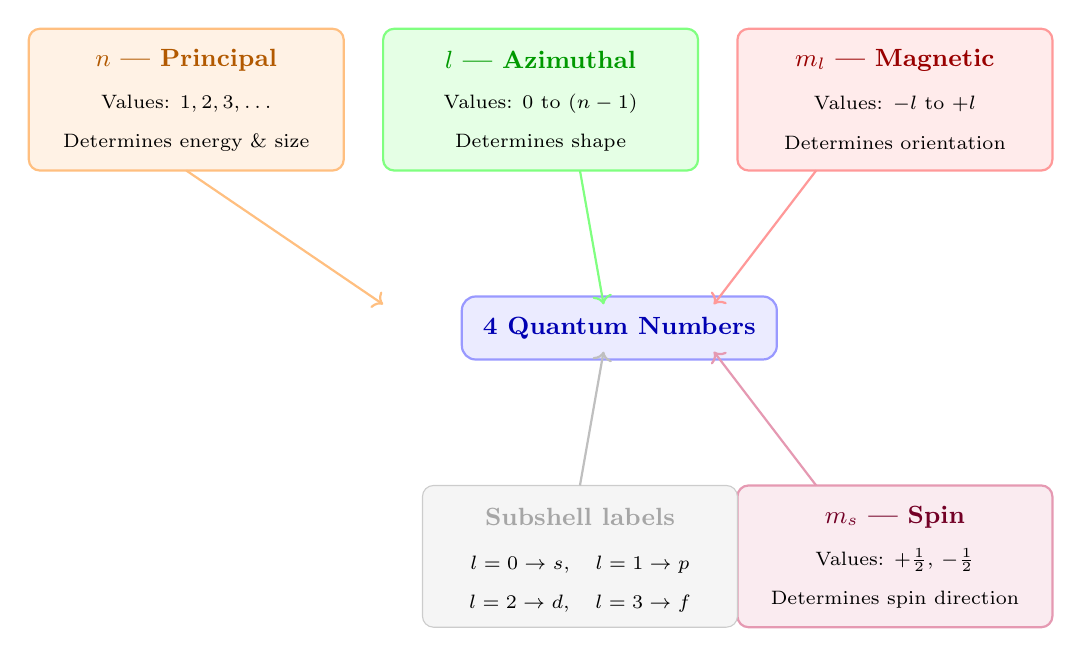
\begin{tikzpicture}[x=1cm, y=1cm]

  %% central node
  \draw[rounded corners=5pt, fill=blue!8, draw=blue!40, thick]
    (0,-0.4) rectangle (4.0,0.4);
  \node[font=\small\bfseries, blue!70!black] at (2.0,0)
    {4 Quantum Numbers};

  %% n
  \draw[rounded corners=4pt, fill=orange!10, draw=orange!50, thick]
    (-5.5, 2.0) rectangle (-1.5, 3.8);
  \node[font=\small\bfseries, orange!70!black] at (-3.5,3.4)
    {$n$ — Principal};
  \node[font=\scriptsize, align=center] at (-3.5,2.85)
    {Values: $1,2,3,\ldots$};
  \node[font=\scriptsize, align=center] at (-3.5,2.35)
    {Determines energy \& size};
  \draw[->, thick, orange!50] (-3.5,2.0) -- (-1.0, 0.3);

  %% l
  \draw[rounded corners=4pt, fill=green!10, draw=green!50, thick]
    (-1.0, 2.0) rectangle (3.0, 3.8);
  \node[font=\small\bfseries, green!60!black] at (1.0,3.4)
    {$l$ — Azimuthal};
  \node[font=\scriptsize, align=center] at (1.0,2.85)
    {Values: $0$ to $(n-1)$};
  \node[font=\scriptsize, align=center] at (1.0,2.35)
    {Determines shape};
  \draw[->, thick, green!50] (1.5,2.0) -- (1.8, 0.3);

  %% ml
  \draw[rounded corners=4pt, fill=red!8, draw=red!40, thick]
    (3.5, 2.0) rectangle (7.5, 3.8);
  \node[font=\small\bfseries, red!60!black] at (5.5,3.4)
    {$m_l$ — Magnetic};
  \node[font=\scriptsize, align=center] at (5.5,2.85)
    {Values: $-l$ to $+l$};
  \node[font=\scriptsize, align=center] at (5.5,2.35)
    {Determines orientation};
  \draw[->, thick, red!40] (4.5,2.0) -- (3.2, 0.3);

  %% ms
  \draw[rounded corners=4pt, fill=purple!8, draw=purple!40, thick]
    (3.5,-2.0) rectangle (7.5,-3.8);
  \node[font=\small\bfseries, purple!60!black] at (5.5,-2.4)
    {$m_s$ — Spin};
  \node[font=\scriptsize, align=center] at (5.5,-2.95)
    {Values: $+\tfrac{1}{2},\,-\tfrac{1}{2}$};
  \node[font=\scriptsize, align=center] at (5.5,-3.45)
    {Determines spin direction};
  \draw[->, thick, purple!40] (4.5,-2.0) -- (3.2,-0.3);

  %% l subshell labels
  \draw[rounded corners=4pt, fill=gray!8, draw=gray!40]
    (-0.5,-2.0) rectangle (3.5,-3.8);
  \node[font=\small\bfseries, gray!70] at (1.5,-2.4)
    {Subshell labels};
  \node[font=\scriptsize] at (1.5,-3.0)
    {$l=0\to s,\quad l=1\to p$};
  \node[font=\scriptsize] at (1.5,-3.5)
    {$l=2\to d,\quad l=3\to f$};
  \draw[->, thick, gray!50] (1.5,-2.0) -- (1.8,-0.3);

\end{tikzpicture}
\end{center}

\bigskip
\textbf{2. Three Rules for Building Configurations:}

\bigskip
\textbf{Rule 1 — Aufbau Principle:}
Electrons fill orbitals in order of \textbf{increasing energy}.
The filling order follows the $(n+l)$ rule — lower $(n+l)$ fills
first; if equal, lower $n$ fills first:

\begin{center}
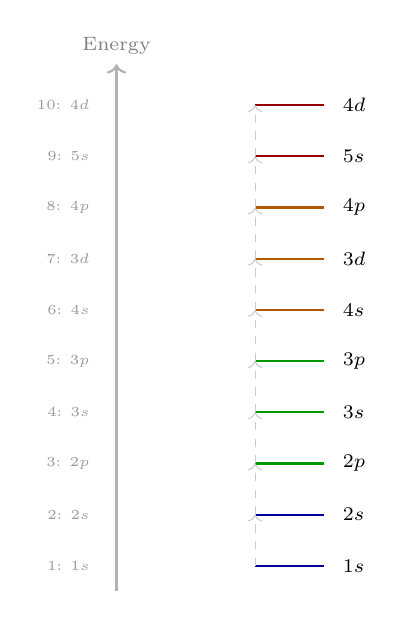
\begin{tikzpicture}[x=1.1cm, y=0.65cm]

  %% orbital energy level diagram
  \def\orb#1#2#3{
    \draw[thick, #3] (#1-0.4,#2) -- (#1+0.4,#2);
  }

  %% levels with colour coding
  \orb{1}{0}{blue!60!black}  \node[right, font=\scriptsize] at (1.5, 0)  {$1s$};
  \orb{1}{1}{blue!60!black}  \node[right, font=\scriptsize] at (1.5, 1)  {$2s$};
  \orb{1}{2}{green!60!black} \node[right, font=\scriptsize] at (1.5, 2)  {$2p$};
  \orb{1}{3}{green!60!black} \node[right, font=\scriptsize] at (1.5, 3)  {$3s$};
  \orb{1}{4}{green!60!black} \node[right, font=\scriptsize] at (1.5, 4)  {$3p$};
  \orb{1}{5}{orange!70!black}\node[right, font=\scriptsize] at (1.5, 5)  {$4s$};
  \orb{1}{6}{orange!70!black}\node[right, font=\scriptsize] at (1.5, 6)  {$3d$};
  \orb{1}{7}{orange!70!black}\node[right, font=\scriptsize] at (1.5, 7)  {$4p$};
  \orb{1}{8}{red!60!black}   \node[right, font=\scriptsize] at (1.5, 8)  {$5s$};
  \orb{1}{9}{red!60!black}   \node[right, font=\scriptsize] at (1.5, 9)  {$4d$};

  %% energy axis
  \draw[->, thick, gray!60] (-1.0,-0.5) -- (-1.0, 9.8)
    node[above, font=\scriptsize, gray] {Energy};

  %% diagonal arrows showing filling order
  \foreach \y/\label in {
    0/{1: $1s$},
    1/{2: $2s$},
    2/{3: $2p$},
    3/{4: $3s$},
    4/{5: $3p$},
    5/{6: $4s$},
    6/{7: $3d$},
    7/{8: $4p$},
    8/{9: $5s$},
    9/{10: $4d$}
  }{
    \node[left, font=\tiny, gray!80] at (-1.2, \y) {\label};
  }

  %% filling order diagonal arrows
  \draw[->, dashed, gray!40, thin]
    (0.6,0) -- (0.6,1);
  \draw[->, dashed, gray!40, thin]
    (0.6,1) -- (0.6,2);
  \draw[->, dashed, gray!40, thin]
    (0.6,2) -- (0.6,3);
  \draw[->, dashed, gray!40, thin]
    (0.6,3) -- (0.6,4);
  \draw[->, dashed, gray!40, thin]
    (0.6,4) -- (0.6,5);
  \draw[->, dashed, gray!40, thin]
    (0.6,5) -- (0.6,6);
  \draw[->, dashed, gray!40, thin]
    (0.6,6) -- (0.6,7);
  \draw[->, dashed, gray!40, thin]
    (0.6,7) -- (0.6,8);
  \draw[->, dashed, gray!40, thin]
    (0.6,8) -- (0.6,9);

\end{tikzpicture}
\end{center}

\textbf{Rule 2 — Pauli Exclusion Principle:}
No two electrons in an atom can have the same four quantum numbers.
Each orbital holds \textbf{at most 2 electrons} with opposite spins:

\begin{center}
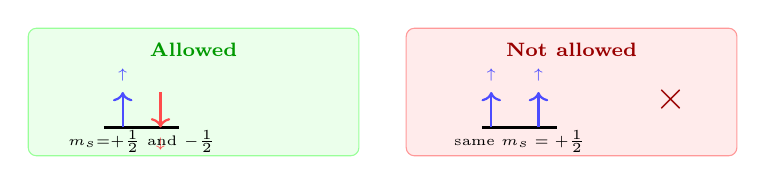
\begin{tikzpicture}[x=1.2cm, y=0.9cm]

  %% Allowed
  \draw[rounded corners=3pt, fill=green!8, draw=green!40]
    (0,0) rectangle (3.5,1.8);
  \node[font=\scriptsize\bfseries, green!60!black] at (1.75,1.5)
    {Allowed};
  \draw[thick] (0.8,0.4) -- (1.6,0.4);
  \draw[->, thick, blue!70] (1.0,0.4) -- (1.0,0.9)
    node[above, font=\tiny] {$\uparrow$};
  \draw[->, thick, red!70]  (1.4,0.9) -- (1.4,0.4)
    node[below, font=\tiny] {$\downarrow$};
  \node[font=\tiny] at (1.2,0.2)
    {$m_s{=}{+}\tfrac{1}{2}$ and $-\tfrac{1}{2}$};

  %% Not allowed
  \draw[rounded corners=3pt, fill=red!8, draw=red!40]
    (4.0,0) rectangle (7.5,1.8);
  \node[font=\scriptsize\bfseries, red!60!black] at (5.75,1.5)
    {Not allowed};
  \draw[thick] (4.8,0.4) -- (5.6,0.4);
  \draw[->, thick, blue!70] (4.9,0.4) -- (4.9,0.9)
    node[above, font=\tiny] {$\uparrow$};
  \draw[->, thick, blue!70] (5.4,0.4) -- (5.4,0.9)
    node[above, font=\tiny] {$\uparrow$};
  \node[font=\tiny] at (5.2,0.2)
    {same $m_s = +\tfrac{1}{2}$};
  \node[red!60!black, font=\Large] at (6.8, 0.8) {$\times$};

\end{tikzpicture}
\end{center}

\textbf{Rule 3 — Hund's Rule of Maximum Multiplicity:}
In degenerate orbitals (same $n$ and $l$), electrons occupy
\textbf{separate orbitals} with \textbf{parallel spins} before
pairing:

\begin{center}
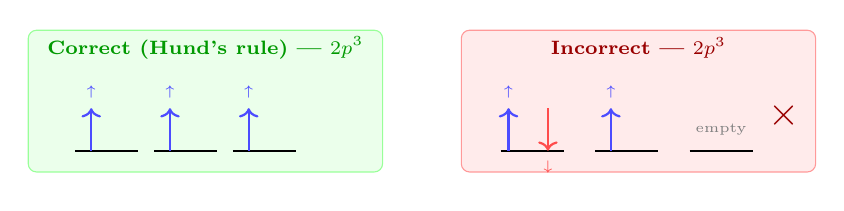
\begin{tikzpicture}[x=1.0cm, y=0.9cm]

  %% Correct - Hund's rule
  \draw[rounded corners=3pt, fill=green!8, draw=green!40]
    (0,0) rectangle (4.5,2.0);
  \node[font=\scriptsize\bfseries, green!60!black] at (2.25,1.75)
    {Correct (Hund's rule) — $2p^3$};
  \foreach \x in {0.6, 1.6, 2.6}{
    \draw[thick] (\x, 0.3) -- (\x+0.8, 0.3);
    \draw[->, thick, blue!70] (\x+0.2, 0.3) -- (\x+0.2, 0.9)
      node[above, font=\tiny]{$\uparrow$};
  }

  %% Incorrect
  \draw[rounded corners=3pt, fill=red!8, draw=red!40]
    (5.5,0) rectangle (10.0,2.0);
  \node[font=\scriptsize\bfseries, red!60!black] at (7.75,1.75)
    {Incorrect — $2p^3$};
  \draw[thick] (6.0,0.3) -- (6.8,0.3);
  \draw[->, thick, blue!70] (6.1,0.3) -- (6.1,0.9)
    node[above, font=\tiny]{$\uparrow$};
  \draw[->, thick, red!70]  (6.6,0.9) -- (6.6,0.3)
    node[below, font=\tiny]{$\downarrow$};
  \draw[thick] (7.2,0.3) -- (8.0,0.3);
  \draw[->, thick, blue!70] (7.4,0.3) -- (7.4,0.9)
    node[above, font=\tiny]{$\uparrow$};
  \draw[thick] (8.4,0.3) -- (9.2,0.3);
  \node[font=\tiny, gray] at (8.8,0.6) {empty};
  \node[red!60!black, font=\Large] at (9.6,0.8) {$\times$};

\end{tikzpicture}
\end{center}

\bigskip
\textbf{3. Worked Example — Carbon ($Z=6$):}

\begin{center}
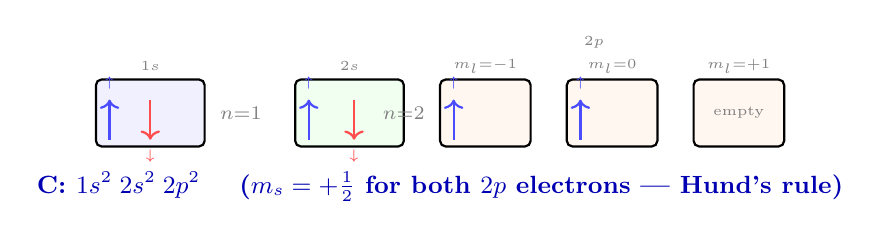
\begin{tikzpicture}[x=1.15cm, y=0.85cm]

  %% 1s box
  \draw[thick, rounded corners=2pt, fill=blue!6]
    (0,0) rectangle (1.2,1.0);
  \node[font=\tiny, gray] at (0.6,1.2) {$1s$};
  \draw[->, thick, blue!70] (0.15,0.1) -- (0.15,0.7)
    node[above, font=\tiny]{$\uparrow$};
  \draw[->, thick, red!70]  (0.6, 0.7) -- (0.6, 0.1)
    node[below, font=\tiny]{$\downarrow$};

  \node[font=\scriptsize, gray] at (1.6,0.5) {$n{=}1$};

  %% 2s box
  \draw[thick, rounded corners=2pt, fill=green!6]
    (2.2,0) rectangle (3.4,1.0);
  \node[font=\tiny, gray] at (2.8,1.2) {$2s$};
  \draw[->, thick, blue!70] (2.35,0.1) -- (2.35,0.7)
    node[above, font=\tiny]{$\uparrow$};
  \draw[->, thick, red!70]  (2.85,0.7) -- (2.85,0.1)
    node[below, font=\tiny]{$\downarrow$};

  %% 2p boxes
  \foreach \i/\ml in {0/$m_l{=}{-1}$,1/$m_l{=}0$,2/$m_l{=}{+1}$}{
    \draw[thick, rounded corners=2pt, fill=orange!6]
      ({3.8+\i*1.4},0) rectangle ({4.8+\i*1.4},1.0);
    \node[font=\tiny, gray] at ({4.3+\i*1.4},1.2) {\ml};
  }
  \node[font=\tiny, gray] at (5.5,1.55) {$2p$};

  %% one electron in each of first two 2p orbitals (Hund's rule)
  \draw[->, thick, blue!70] (3.95,0.1) -- (3.95,0.7)
    node[above, font=\tiny]{$\uparrow$};
  \draw[->, thick, blue!70] (5.35,0.1) -- (5.35,0.7)
    node[above, font=\tiny]{$\uparrow$};
  \node[font=\tiny, gray]   at (7.1,0.5)  {empty};

  \node[font=\scriptsize, gray] at (3.4,0.5) {$n{=}2$};

  %% Configuration label
  \node[font=\small\bfseries, blue!70!black] at (3.8,-0.6)
    {C: $1s^2\;2s^2\;2p^2$
     \quad ($m_s = +\tfrac{1}{2}$ for both $2p$ electrons — Hund's rule)};

\end{tikzpicture}
\end{center}

\bigskip
\textbf{4. Quantum Numbers for Each Electron in Carbon:}

\begin{center}
\begin{tabular}{p{1.8cm} p{1.2cm} p{1.2cm} p{1.8cm} p{2.0cm}
                p{2.5cm}}
\toprule
\textbf{Electron} & \textbf{$n$} & \textbf{$l$} &
\textbf{$m_l$} & \textbf{$m_s$} & \textbf{Orbital} \\
\midrule
1 & 1 & 0 & 0  & $+\tfrac{1}{2}$ & $1s$ \\[2pt]
2 & 1 & 0 & 0  & $-\tfrac{1}{2}$ & $1s$ \\[2pt]
3 & 2 & 0 & 0  & $+\tfrac{1}{2}$ & $2s$ \\[2pt]
4 & 2 & 0 & 0  & $-\tfrac{1}{2}$ & $2s$ \\[2pt]
5 & 2 & 1 & $-1$ & $+\tfrac{1}{2}$ & $2p$ (Hund) \\[2pt]
6 & 2 & 1 & $0$  & $+\tfrac{1}{2}$ & $2p$ (Hund) \\
\bottomrule
\end{tabular}
\end{center}

\bigskip
\textbf{Conclusion:} Electron configurations are built by applying
the \textbf{Aufbau principle} (fill lowest energy first),
\textbf{Pauli exclusion principle} (no two electrons share all four
quantum numbers), and \textbf{Hund's rule} (maximise parallel spins
in degenerate orbitals). Together, the four quantum numbers
$(n, l, m_l, m_s)$ uniquely identify every electron in an atom and
completely define its energy, orbital shape, orientation, and spin.
\end{tcolorbox}

\item Draw a rough sketch of a periodic table (no details required). Indicate where alkali metals, chalcogens and halogens are located. Write the name and symbol for an element in each of these groups. \mk{--}
\yr{CHEM 113 | 2014--15}

\begin{tcolorbox}[enhanced,breakable,ansbox,colback=cA!4,colframe=cA,boxrule=0.8pt,arc=5pt,title={\textbf{Answer}},fonttitle=\bfseries\color{white},colbacktitle=cA]

\begin{center}
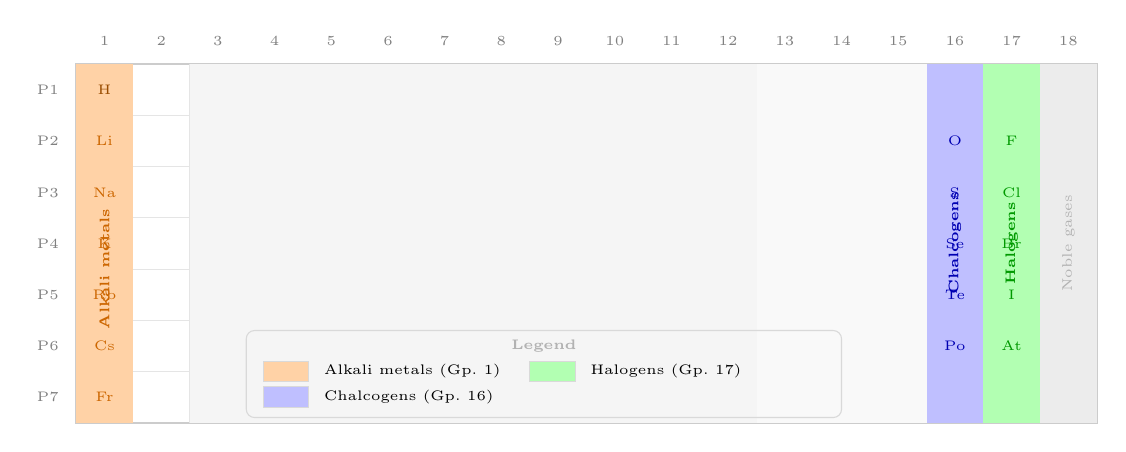
\begin{tikzpicture}[x=0.72cm, y=0.65cm]

  %% ── Main periodic table outline ──────────────────────────────
  \draw[gray!40, thick] (0,0) rectangle (18,-7);

  %% Group dividers
  \foreach \x in {1,2,3,4,5,6,7,8,9,10,11,12,13,14,15,16,17}{
    \draw[gray!20, thin] (\x,0) -- (\x,-7);
  }
  %% Period dividers
  \foreach \y in {-1,-2,-3,-4,-5,-6}{
    \draw[gray!20, thin] (0,\y) -- (18,\y);
  }

  %% ── Period labels ─────────────────────────────────────────────
  \foreach \y/\p in {0/1,-1/2,-2/3,-3/4,-4/5,-5/6,-6/7}{
    \node[font=\tiny, gray] at (-0.5,{\y-0.5}) {P\p};
  }

  %% ── Group labels ──────────────────────────────────────────────
  \foreach \x/\g in {0/1,1/2,2/3,3/4,4/5,5/6,6/7,7/8,8/9,
                     9/10,10/11,11/12,12/13,13/14,14/15,
                     15/16,16/17,17/18}{
    \node[font=\tiny, gray] at ({\x+0.5},0.45) {\g};
  }

  %% ── General block fills (subtle) ─────────────────────────────
  \fill[gray!8] (2,0) rectangle (12,-7);   %% d-block
  \fill[gray!5] (12,0) rectangle (18,-7);  %% p-block

  %% ── Alkali metals — Group 1 (col 0), periods 2-7 ─────────────
  \fill[orange!35] (0,-1) rectangle (1,-7);
  \node[font=\tiny, orange!80!black, rotate=90] at (0.5,-4.0)
    {\textbf{Alkali metals}};

  %% ── Chalcogens — Group 16 (col 15), all periods ──────────────
  \fill[blue!25] (15,0) rectangle (16,-7);
  \node[font=\tiny, blue!70!black, rotate=90] at (15.5,-3.5)
    {\textbf{Chalcogens}};

  %% ── Halogens — Group 17 (col 16), all periods ────────────────
  \fill[green!30] (16,0) rectangle (17,-7);
  \node[font=\tiny, green!60!black, rotate=90] at (16.5,-3.5)
    {\textbf{Halogens}};

  %% ── Noble gases (col 17) subtle fill for context ─────────────
  \fill[gray!15] (17,0) rectangle (18,-7);
  \node[font=\tiny, gray!60, rotate=90] at (17.5,-3.5)
    {Noble gases};

  %% ── Hydrogen special case label ──────────────────────────────
  \fill[orange!35] (0,0) rectangle (1,-1);
  \node[font=\tiny, orange!60!black] at (0.5,-0.5) {H};

  %% ── Example element labels inside highlighted columns ─────────

  %% Alkali metals examples
  \node[font=\tiny, orange!80!black] at (0.5,-1.5) {Li};
  \node[font=\tiny, orange!80!black] at (0.5,-2.5) {Na};
  \node[font=\tiny, orange!80!black] at (0.5,-3.5) {K};
  \node[font=\tiny, orange!80!black] at (0.5,-4.5) {Rb};
  \node[font=\tiny, orange!80!black] at (0.5,-5.5) {Cs};
  \node[font=\tiny, orange!80!black] at (0.5,-6.5) {Fr};

  %% Chalcogens examples
  \node[font=\tiny, blue!70!black] at (15.5,-1.5) {O};
  \node[font=\tiny, blue!70!black] at (15.5,-2.5) {S};
  \node[font=\tiny, blue!70!black] at (15.5,-3.5) {Se};
  \node[font=\tiny, blue!70!black] at (15.5,-4.5) {Te};
  \node[font=\tiny, blue!70!black] at (15.5,-5.5) {Po};

  %% Halogens examples
  \node[font=\tiny, green!60!black] at (16.5,-1.5) {F};
  \node[font=\tiny, green!60!black] at (16.5,-2.5) {Cl};
  \node[font=\tiny, green!60!black] at (16.5,-3.5) {Br};
  \node[font=\tiny, green!60!black] at (16.5,-4.5) {I};
  \node[font=\tiny, green!60!black] at (16.5,-5.5) {At};

  %% ── Legend (inside box, bottom centre) ───────────────────────
  \draw[rounded corners=3pt, gray!30, thin]
    (3.0,-5.2) rectangle (13.5,-6.9);
  \node[font=\tiny\bfseries, gray!60] at (8.25,-5.5)
    {Legend};

  %% Alkali metals
  \fill[orange!35] (3.3,-5.8) rectangle (4.1,-6.2);
  \draw[gray!30, thin] (3.3,-5.8) rectangle (4.1,-6.2);
  \node[right, font=\tiny] at (4.2,-6.0)
    {Alkali metals (Gp.\ 1)};

  %% Chalcogens
  \fill[blue!25] (3.3,-6.3) rectangle (4.1,-6.7);
  \draw[gray!30, thin] (3.3,-6.3) rectangle (4.1,-6.7);
  \node[right, font=\tiny] at (4.2,-6.5)
    {Chalcogens (Gp.\ 16)};

  %% Halogens
  \fill[green!30] (8.0,-5.8) rectangle (8.8,-6.2);
  \draw[gray!30, thin] (8.0,-5.8) rectangle (8.8,-6.2);
  \node[right, font=\tiny] at (8.9,-6.0)
    {Halogens (Gp.\ 17)};

\end{tikzpicture}
\end{center}

\bigskip
\textbf{Named Elements in Each Group:}

\begin{center}
\begin{tabular}{p{3.0cm} p{2.5cm} p{2.5cm} p{4.5cm}}
\toprule
\textbf{Group} & \textbf{Group No.} & \textbf{Element} &
\textbf{Properties} \\
\midrule
Alkali metals
  & 1
  & Sodium (Na)
  & Soft, silvery metal; reacts vigorously with water \\[4pt]
Chalcogens
  & 16
  & Oxygen (O)
  & Colourless gas; essential for combustion and respiration \\[4pt]
Halogens
  & 17
  & Chlorine (Cl)
  & Toxic yellow-green gas; strong oxidising agent \\
\bottomrule
\end{tabular}
\end{center}

\textbf{Key observations:}
\begin{itemize}
  \item \textbf{Alkali metals} (Group 1) occupy the far left column.
        They have one valence electron ($ns^1$) and are the most
        reactive metals — reactivity \textit{increases} down the group.
  \item \textbf{Chalcogens} (Group 16) are two columns from the
        right. They have six valence electrons ($ns^2np^4$) and
        commonly form $-2$ anions or covalent bonds.
  \item \textbf{Halogens} (Group 17) occupy the second-to-last
        column. They have seven valence electrons ($ns^2np^5$),
        need only one more electron to complete their octet, and
        are the most reactive non-metals — reactivity
        \textit{decreases} down the group.
\end{itemize}

\end{tcolorbox}

\item Explain with a figure how each of these properties of the representative elements generally increases or decreases across the periodic table: (i) atomic size, (ii) electron affinity, (iii) ionization energy, (iv) metallic character, (v) acidity of oxides. \mk{12}
\yr{CHEM 113 | 2014--15}

\begin{tcolorbox}[enhanced,breakable,ansbox,colback=cA!4,colframe=cA,boxrule=0.8pt,arc=5pt,title={\textbf{Answer}},fonttitle=\bfseries\color{white},colbacktitle=cA]

\begin{center}
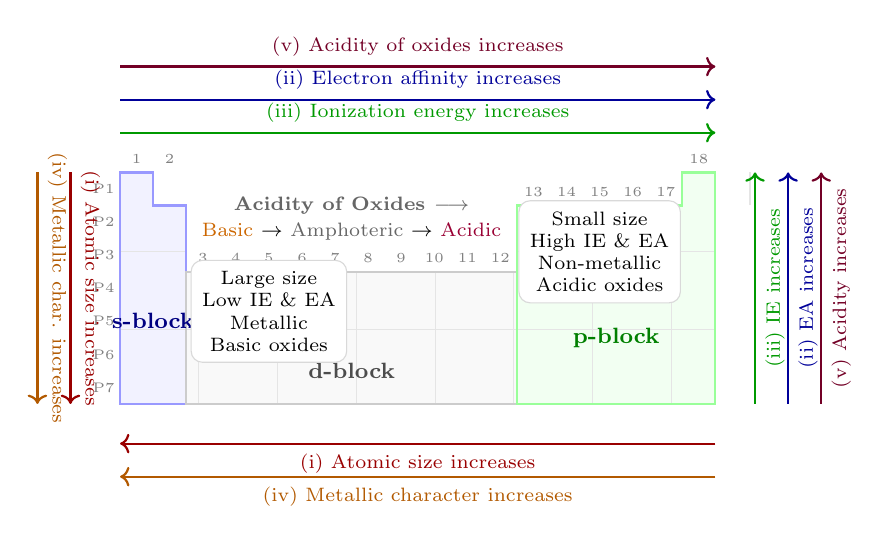
\begin{tikzpicture}[x=0.42cm, y=0.42cm]

  %% ── Block Fills ──────────────────────────────────────────────
  \fill[blue!5] (0,0) -- (1,0) -- (1,-1) -- (2,-1) -- (2,-7) -- (0,-7) -- cycle;
  \fill[gray!5] (2,-3) rectangle (12,-7);
  \fill[green!5] (17,0) -- (18,0) -- (18,-7) -- (12,-7) -- (12,-1) -- (17,-1) -- cycle;

  %% ── Faint Grid Lines ─────────────────────────────────────────
  %% s-block
  \draw[gray!20, thin] (0,0) grid (1,-1);
  \draw[gray!20, thin] (0,-1) grid (2,-7);
  %% d-block
  \draw[gray!20, thin] (2,-3) grid (12,-7);
  %% p-block
  \draw[gray!20, thin] (17,0) grid (18,-1);
  \draw[gray!20, thin] (12,-1) grid (18,-7);

  %% ── Thick Block Outlines ─────────────────────────────────────
  \draw[blue!40, thick] (0,0) -- (1,0) -- (1,-1) -- (2,-1) -- (2,-7) -- (0,-7) -- cycle;
  \draw[gray!40, thick] (2,-3) rectangle (12,-7);
  \draw[green!40, thick] (17,0) -- (18,0) -- (18,-7) -- (12,-7) -- (12,-1) -- (17,-1) -- cycle;

  %% ── Labels inside the grid ───────────────────────────────────
  %% Period labels
  \foreach \y/\p in {0/1,-1/2,-2/3,-3/4,-4/5,-5/6,-6/7} {
    \node[font=\tiny, gray] at (-0.5, \y-0.5) {P\p};
  }
  %% Group labels
  \foreach \x in {1,2} \node[font=\tiny, gray] at (\x-0.5, 0.4) {\x};
  \foreach \x in {13,14,15,16,17} \node[font=\tiny, gray] at (\x-0.5, -0.6) {\x};
  \node[font=\tiny, gray] at (17.5, 0.4) {18};
  \foreach \x in {3,4,5,6,7,8,9,10,11,12} \node[font=\tiny, gray] at (\x-0.5, -2.6) {\x};

  %% Block Names
  \node[font=\footnotesize\bfseries, blue!50!black] at (1, -4.5) {s-block};
  \node[font=\footnotesize\bfseries, gray!60!black] at (7, -6.0) {d-block};
  \node[font=\footnotesize\bfseries, green!50!black] at (15, -5.0) {p-block};

  %% Acidity Gradient (in empty space)
  \node[font=\scriptsize\bfseries, gray!80!black] at (7, -1.0) {Acidity of Oxides $\longrightarrow$};
  \node[font=\scriptsize] at (7, -1.8) {\textcolor{orange!80!black}{Basic} $\rightarrow$ \textcolor{gray!80!black}{Amphoteric} $\rightarrow$ \textcolor{purple!80!black}{Acidic}};

  %% ── Corner Summary Boxes ─────────────────────────────────────
  %% Bottom-Left
  \node[font=\scriptsize, align=center, fill=white, draw=gray!30, rounded corners, inner sep=4pt] 
    at (4.5, -4.2) {Large size\\Low IE \& EA\\Metallic\\Basic oxides};
  
  %% Top-Right
  \node[font=\scriptsize, align=center, fill=white, draw=gray!30, rounded corners, inner sep=4pt] 
    at (14.5, -2.4) {Small size\\High IE \& EA\\Non-metallic\\Acidic oxides};

  %% ═══════════════════════════════════════════════════════════
  %%  TREND ARROWS — placed neatly OUTSIDE the grid
  %% ═══════════════════════════════════════════════════════════

  %% Top Arrows (Across Period ->)
  \draw[->, thick, green!60!black] (0, 1.2) -- (18, 1.2) 
    node[midway, above, font=\scriptsize] {(iii) Ionization energy increases};
  \draw[->, thick, blue!60!black]  (0, 2.2) -- (18, 2.2) 
    node[midway, above, font=\scriptsize] {(ii) Electron affinity increases};
  \draw[->, thick, purple!60!black] (0, 3.2) -- (18, 3.2) 
    node[midway, above, font=\scriptsize] {(v) Acidity of oxides increases};

  %% Bottom Arrows (Across Period <-)
  \draw[->, thick, red!60!black]    (18, -8.2) -- (0, -8.2) 
    node[midway, below, font=\scriptsize] {(i) Atomic size increases};
  \draw[->, thick, orange!70!black] (18, -9.2) -- (0, -9.2) 
    node[midway, below, font=\scriptsize] {(iv) Metallic character increases};

  %% Right Arrows (Down Group ^)
  \draw[->, thick, green!60!black]  (19.2, -7) -- (19.2, 0) 
    node[midway, below, sloped, font=\scriptsize] {(iii) IE increases};
  \draw[->, thick, blue!60!black]   (20.2, -7) -- (20.2, 0) 
    node[midway, below, sloped, font=\scriptsize] {(ii) EA increases};
  \draw[->, thick, purple!60!black] (21.2, -7) -- (21.2, 0) 
    node[midway, below, sloped, font=\scriptsize] {(v) Acidity increases};

  %% Left Arrows (Down Group v)
  \draw[->, thick, red!60!black]    (-1.5, 0) -- (-1.5, -7) 
    node[midway, above, sloped, font=\scriptsize] {(i) Atomic size increases};
  \draw[->, thick, orange!70!black] (-2.5, 0) -- (-2.5, -7) 
    node[midway, above, sloped, font=\scriptsize] {(iv) Metallic char. increases};

\end{tikzpicture}
\end{center}

\bigskip
\textbf{(i) Atomic Size:}

Atomic size is the distance from the nucleus to the outermost electron.
\begin{itemize}
  \item \textbf{Across a period} ($\rightarrow$): nuclear charge $Z$
        increases with minimal extra shielding, pulling electrons
        inward $\Rightarrow$ \textbf{atomic size decreases}.
  \item \textbf{Down a group} ($\downarrow$): new electron shells are
        added, increasing shielding $\Rightarrow$
        \textbf{atomic size increases}.
  \item Largest: Fr ($\sim$270 pm); Smallest: He ($\sim$31 pm).
\end{itemize}

\bigskip
\textbf{(ii) Electron Affinity (EA):}

EA is the energy released when a gaseous atom gains one electron:
$\text{M}_{(g)} + e^- \rightarrow \text{M}^-_{(g)}$
\begin{itemize}
  \item \textbf{Across a period} ($\rightarrow$): increasing
        $Z_{\text{eff}}$ attracts electrons more strongly
        $\Rightarrow$ \textbf{EA increases} (more negative).
        Exceptions: group 2 (filled $2s^2$) and group 5
        (half-filled $p^3$) show anomalously low EA.
  \item \textbf{Down a group} ($\downarrow$): larger radius and
        greater shielding reduce nuclear attraction
        $\Rightarrow$ \textbf{EA decreases}.
  \item Most negative EA: Cl ($-349$ kJ/mol).
\end{itemize}

\bigskip
\textbf{(iii) Ionization Energy (IE):}

IE is the energy required to remove the outermost electron:
$\text{M}_{(g)} \rightarrow \text{M}^+_{(g)} + e^-$
\begin{itemize}
  \item \textbf{Across a period} ($\rightarrow$): increasing
        $Z_{\text{eff}}$ holds electrons more tightly
        $\Rightarrow$ \textbf{IE increases}.
        Exceptions: slight dip at group 13 (Al $<$ Mg, due to
        $2p > 2s$) and group 16 (S $<$ P, due to pairing
        repulsion).
  \item \textbf{Down a group} ($\downarrow$): outer electrons are
        farther away and more shielded $\Rightarrow$
        \textbf{IE decreases}.
  \item Highest: He ($2372$ kJ/mol); Lowest: Cs ($376$ kJ/mol).
\end{itemize}

\bigskip
\textbf{(iv) Metallic Character:}

Metallic character reflects the tendency to lose electrons and form
cations — directly linked to low IE and large atomic radius.
\begin{itemize}
  \item \textbf{Across a period} ($\rightarrow$): IE increases,
        electron loss becomes harder $\Rightarrow$
        \textbf{metallic character decreases}
        (metals on left, non-metals on right).
  \item \textbf{Down a group} ($\downarrow$): IE decreases, electrons
        lost more easily $\Rightarrow$
        \textbf{metallic character increases}.
  \item Most metallic: Fr; Least metallic: F.
\end{itemize}

\bigskip
\textbf{(v) Acidity of Oxides:}

The nature of element oxides shifts systematically across the table:
\[
  \underbrace{\text{Na}_2\text{O},\;\text{MgO}}_{\text{basic}}
  \;\longrightarrow\;
  \underbrace{\text{Al}_2\text{O}_3}_{\text{amphoteric}}
  \;\longrightarrow\;
  \underbrace{\text{SiO}_2,\;\text{P}_2\text{O}_5,\;
              \text{SO}_3,\;\text{Cl}_2\text{O}_7}_{\text{acidic}}
\]
\begin{itemize}
  \item \textbf{Across a period} ($\rightarrow$): as metallic
        character decreases, oxides change from
        \textbf{basic} (ionic, e.g.\ Na$_2$O) through
        \textbf{amphoteric} (e.g.\ Al$_2$O$_3$) to
        \textbf{acidic} (covalent, e.g.\ Cl$_2$O$_7$).
  \item \textbf{Down a group} ($\downarrow$): metallic character
        increases $\Rightarrow$ oxides become \textbf{more basic}.
        E.g.\ in group 14: CO$_2$ (acidic) $\rightarrow$
        SnO$_2$ (amphoteric) $\rightarrow$ PbO (basic).
  \item The shift from basic to acidic oxide reflects the
        increasing $Z_{\text{eff}}$ and covalent bonding character
        of the element--oxygen bond across a period.
\end{itemize}

\bigskip
\textbf{Summary Table:}
\begin{center}
\begin{tabular}{p{3.5cm} p{2.8cm} p{2.8cm}}
\toprule
\textbf{Property} &
\textbf{Across period} ($\rightarrow$) &
\textbf{Down group} ($\downarrow$) \\
\midrule
(i)\ \ Atomic size        & Decreases   & Increases \\[3pt]
(ii)\ \ Electron affinity & Increases   & Decreases \\[3pt]
(iii)\ Ionization energy  & Increases   & Decreases \\[3pt]
(iv)\ \ Metallic character& Decreases   & Increases \\[3pt]
(v)\ \ Acidity of oxides  & Increases   & Decreases \\
\bottomrule
\end{tabular}
\end{center}

\textbf{Conclusion:} All five properties are governed by the
interplay of \textbf{nuclear charge}, \textbf{electron shielding},
and \textbf{atomic radius}. Increasing $Z_{\text{eff}}$ across a
period shrinks atoms, raises IE and EA, reduces metallic character,
and shifts oxide character from basic to acidic. The reverse holds
going down a group as shielding dominates.

\end{tcolorbox}

\item Give a brief description of the wave nature of light. What are the two main characteristics of light wave?\mk{4}
\yr{CHEM 113 | 2014-15}

\begin{tcolorbox}[enhanced,breakable,ansbox,colback=cA!4,colframe=cA,boxrule=0.8pt,arc=5pt,title={\textbf{Answer}},fonttitle=\bfseries\color{white},colbacktitle=cA]
\textbf{Wave Nature of Light:}

Light is an \textbf{electromagnetic wave} consisting of oscillating electric and magnetic fields propagating perpendicular to each other and to the direction of travel. This wave nature was established by Maxwell (1865) and confirmed by Hertz (1887). It travels through vacuum at:
\[
  c = 3.0 \times 10^8 \text{ m/s}
\]

\textbf{Two Main Characteristics:}

\begin{enumerate}
  \item \textbf{Wavelength ($\lambda$):} The distance between two consecutive crests (or troughs) of the wave, measured in metres (m) or nanometres (nm). It determines the \textit{colour} of light — visible light spans $\lambda \approx 400$--$700$ nm.

  \item \textbf{Frequency ($\nu$):} The number of wave cycles passing a point per second, measured in Hertz (Hz). It is related to wavelength by:
  \[
    c = \nu\lambda
  \]
  Higher frequency means higher energy, given by Planck's relation $E = h\nu$.
\end{enumerate}
\end{tcolorbox}

\item Give the equiation that relates wave-particle properties of light. Explain the meaning of each symbol in the equation.\mk{4}
\yr{CHEM 113 | 2014-15}

\begin{tcolorbox}[enhanced,breakable,ansbox,colback=cA!4,colframe=cA,boxrule=0.8pt,arc=5pt,title={\textbf{Answer}},fonttitle=\bfseries\color{white},colbacktitle=cA]
The equation that relates the wave and particle properties of light is the \textbf{Planck--Einstein relation}:
\[
  E = h\nu = \frac{hc}{\lambda}
\]

\textbf{Meaning of each symbol:}
\begin{itemize}
  \item $E$ — Energy of a single photon (particle property), measured in Joules (J)
  \item $h$ — Planck's constant $= 6.626 \times 10^{-34}$ J$\cdot$s; the proportionality constant linking energy to frequency
  \item $\nu$ — Frequency of the light wave (wave property), measured in Hz (s$^{-1}$)
  \item $c$ — Speed of light in vacuum $= 3.0 \times 10^8$ m/s
  \item $\lambda$ — Wavelength of the light wave (wave property), measured in metres (m)
\end{itemize}

\textbf{Significance:} The left side ($E$) represents the \textit{particle} nature of light (photon energy), while the right side ($\nu$ and $\lambda$) represents the \textit{wave} nature — thus the equation \textbf{bridges both natures} of light in a single expression.
\end{tcolorbox}

\item What is Heisenberg's Uncertainty principle? Prove that the product of uncertainty in position of an electron with uncertainty in momentum of the same electron is of the order of Planck's constant. \mk{11}
\yr{CHEM 113 | 2013--14}

\begin{tcolorbox}[enhanced,breakable,ansbox,colback=cA!4,colframe=cA,boxrule=0.8pt,arc=5pt,title={\textbf{Answer}},fonttitle=\bfseries\color{white},colbacktitle=cA]

\textbf{Heisenberg's Uncertainty Principle \& Proof} \hfill \mk{11}

\medskip
\begin{center}
\textcolor{cA}{\rule{0.85\textwidth}{0.5pt}}
\end{center}

%% ── Part 1 ────────────────────────────────────────────────────────────
\medskip
\textbf{Part 1: Heisenberg's Uncertainty Principle} \hfill \mk{3}

\medskip
\textbf{Statement:} It is fundamentally impossible to determine
\emph{simultaneously} and \emph{precisely} both the position and the
momentum of a subatomic particle. The more precisely one is known,
the less precisely the other can be known. Mathematically:
\[
  \Delta x \cdot \Delta p \;\geq\; \frac{h}{4\pi}
\]
where $\Delta x$ is the uncertainty in position, $\Delta p$ is the
uncertainty in momentum, and $h$ is Planck's constant.

\medskip
\textbf{Other conjugate pairs} governed by the same principle:
\[
  \Delta E \cdot \Delta t \;\geq\; \frac{h}{4\pi}
\]
where $\Delta E$ is uncertainty in energy and $\Delta t$ is uncertainty
in time.

\medskip
\textbf{Key Points:}
\begin{itemize}[leftmargin=1.5em, itemsep=3pt]
  \item This is \emph{not} a limitation of instruments or measurement
        technique --- it is a \textbf{fundamental law of nature}.
  \item It arises because any attempt to measure the position of an
        electron (e.g.\ by shining light on it) disturbs its momentum,
        and vice versa.
  \item For macroscopic objects (baseball, car), $h$ is so tiny relative
        to their mass and momentum that the uncertainty is completely
        negligible. It is only significant at the \textbf{subatomic scale}.
  \item It fundamentally rules out the concept of a definite electron
        orbit (as in Bohr's model) and necessitates the \textbf{quantum
        mechanical probability cloud} picture.
\end{itemize}

\begin{center}
\textcolor{cA}{\rule{0.75\textwidth}{0.4pt}}
\end{center}

%% ── Part 2 ────────────────────────────────────────────────────────────
\medskip
\textbf{Part 2: Proof Using the Gamma-Ray Microscope
(Thought Experiment)} \hfill \mk{8}

\medskip
\textbf{(i) Setup:}

To locate an electron, we must illuminate it with a photon (of wavelength
$\lambda$) and observe the scattered photon through a microscope. Let the
microscope have a lens of half-angle $\theta$ (the semi-angle of the cone
of light entering the lens).

\medskip
\textbf{(ii) Uncertainty in Position ($\Delta x$):}

The resolving power of the microscope limits how precisely the electron's
position can be determined. By Rayleigh's criterion, the minimum
resolvable distance (uncertainty in position) is:
\[
  \Delta x \;\approx\; \frac{\lambda}{\sin\theta}
\]
To reduce $\Delta x$, we need smaller $\lambda$ (higher frequency,
higher energy photons).

\medskip
\textbf{(iii) Uncertainty in Momentum ($\Delta p$):}

The incident photon has momentum $p = h/\lambda$. When the photon
collides with the electron and scatters into the lens (anywhere within
the cone of half-angle $\theta$), it transfers momentum to the electron.
The $x$-component of the scattered photon's momentum lies anywhere in
the range:
\[
  -\frac{h\sin\theta}{\lambda} \;\leq\; p_x \;\leq\;
  +\frac{h\sin\theta}{\lambda}
\]
Therefore the uncertainty in the electron's $x$-momentum is:
\[
  \Delta p \;\approx\; \frac{h\sin\theta}{\lambda}
\]

\medskip
\textbf{(iv) Taking the Product $\Delta x \cdot \Delta p$:}

Multiplying the two uncertainties:
\[
  \Delta x \cdot \Delta p
  \;\approx\;
  \frac{\lambda}{\sin\theta}
  \times
  \frac{h\sin\theta}{\lambda}
\]
\[
  \Delta x \cdot \Delta p \;\approx\; h
\]

A more rigorous quantum mechanical derivation (using wave packets and
Fourier analysis) gives the exact lower bound:
\[
  \boxed{\Delta x \cdot \Delta p \;\geq\; \frac{h}{4\pi}}
\]

\medskip
\textbf{(v) Physical Interpretation of the Trade-off:}

\begin{itemize}[leftmargin=1.5em, itemsep=3pt]
  \item To improve position accuracy, use \textbf{shorter} $\lambda$
        (e.g.\ gamma rays):
        \[
          \lambda \downarrow
          \;\Rightarrow\; \Delta x \downarrow
          \;\Rightarrow\; \frac{h}{\lambda} \uparrow
          \;\Rightarrow\; \Delta p \uparrow
        \]
  \item To improve momentum accuracy, use \textbf{longer} $\lambda$
        (e.g.\ radio waves):
        \[
          \lambda \uparrow
          \;\Rightarrow\; \Delta p \downarrow
          \;\Rightarrow\; \frac{\lambda}{\sin\theta} \uparrow
          \;\Rightarrow\; \Delta x \uparrow
        \]
  \item In both cases, the \emph{product} $\Delta x \cdot \Delta p$
        remains of the order of $h$ --- you gain precision in one only
        at the cost of the other.
\end{itemize}

\medskip
\textbf{(vi) Numerical Verification:}

For an electron confined to an atom, $\Delta x \sim 10^{-10}$ m:
\[
  \Delta p \;\geq\; \frac{h}{4\pi\,\Delta x}
  = \frac{6.626\times10^{-34}}{4\pi \times 10^{-10}}
  \approx 5.27 \times 10^{-25} \text{ kg$\cdot$m/s}
\]
\[
  \Delta x \cdot \Delta p
  = 10^{-10} \times 5.27\times10^{-25}
  = 5.27\times10^{-35}
  \;\approx\; \frac{h}{4\pi}
  \;\sim\; \mathcal{O}(h) \quad \checkmark
\]
This confirms that the product is indeed of the order of Planck's
constant $h = 6.626 \times 10^{-34}$ J$\cdot$s.

\medskip
\begin{center}
\textcolor{cA}{\rule{0.85\textwidth}{0.5pt}}
\end{center}

\medskip
\textbf{Conclusion:} Heisenberg's Uncertainty Principle is not a
measurement artifact but a fundamental quantum law. The gamma-ray
microscope thought experiment elegantly proves that
$\Delta x \cdot \Delta p \approx h$ --- any attempt to reduce one
uncertainty inevitably amplifies the other, and their product is
always of the order of Planck's constant. This irreducible uncertainty
at the quantum level makes the classical concept of a precise electron
trajectory physically impossible.

\end{tcolorbox}

\item Draw emission spectra of hydrogen atom. Why does a hydrogen atom give so many lines in its spectrum although there is only one electron in it? \mk{8}
\yr{CHEM 113 | 2012--13}

\begin{tcolorbox}[enhanced,breakable,ansbox,colback=cA!4,colframe=cA,boxrule=0.8pt,arc=5pt,title={\textbf{Answer}},fonttitle=\bfseries\color{white},colbacktitle=cA]
\textbf{Emission Spectrum of Hydrogen Atom}

\medskip
\textbf{Part 1: Diagram of Emission Spectrum}

\begin{center}
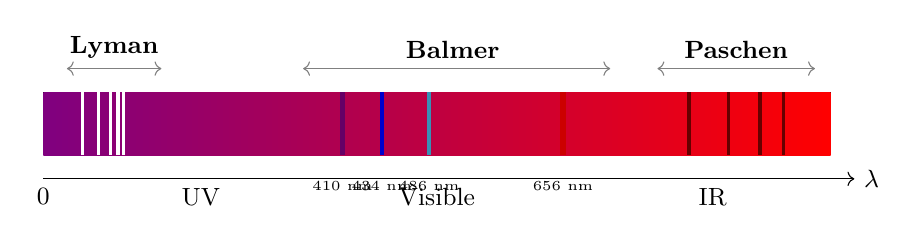
\begin{tikzpicture}[scale=1.0]

  % Draw spectrum bar
  \fill[left color=violet, right color=red] (0,0) rectangle (10,0.8);

  % Lyman series (UV) -- left region
  \foreach \x in {0.5, 0.7, 0.85, 0.95, 1.02}{
    \draw[white, line width=1.2pt] (\x, 0) -- (\x, 0.8);
  }

  % Balmer series (Visible)
  \draw[violet!80!black, line width=1.5pt] (3.8,0) -- (3.8,0.8);  % H-delta 410nm
  \draw[blue!80!black,   line width=1.5pt] (4.3,0) -- (4.3,0.8);  % H-gamma 434nm
  \draw[cyan!70!black,   line width=1.5pt] (4.9,0) -- (4.9,0.8);  % H-beta  486nm
  \draw[red!80!black,    line width=2.0pt] (6.6,0) -- (6.6,0.8);  % H-alpha 656nm

  % Paschen series (IR) -- right region
  \foreach \x in {8.2, 8.7, 9.1, 9.4}{
    \draw[red!40!black, line width=1.2pt] (\x, 0) -- (\x, 0.8);
  }

  % Wavelength axis
  \draw[->] (0,-0.3) -- (10.3,-0.3) node[right]{\small $\lambda$};
  \node[below] at (0,-0.3) {\small 0};
  \node[below] at (2.0,-0.3) {\small UV};
  \node[below] at (5.0,-0.3) {\small Visible};
  \node[below] at (8.5,-0.3) {\small IR};

  % Series labels above
  \draw[<->, gray] (0.3,1.1) -- (1.5,1.1);
  \node[above] at (0.9,1.1) {\small\textbf{Lyman}};

  \draw[<->, gray] (3.3,1.1) -- (7.2,1.1);
  \node[above] at (5.2,1.1) {\small\textbf{Balmer}};

  \draw[<->, gray] (7.8,1.1) -- (9.8,1.1);
  \node[above] at (8.8,1.1) {\small\textbf{Paschen}};

  % Balmer line labels
  \node[below=6pt, font=\tiny] at (3.8,0) {410 nm};
  \node[below=6pt, font=\tiny] at (4.3,0) {434 nm};
  \node[below=6pt, font=\tiny] at (4.9,0) {486 nm};
  \node[below=6pt, font=\tiny] at (6.6,0) {656 nm};

\end{tikzpicture}
\end{center}

\medskip
\textbf{Part 2: Energy Level Transitions}

\begin{center}
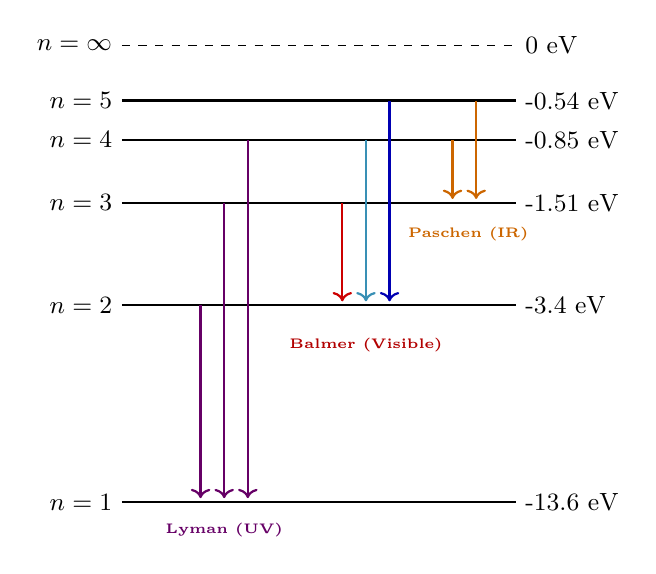
\begin{tikzpicture}[scale=1.0]
  % Energy levels
  \foreach \n/\y/\E in {1/0/{-13.6 eV}, 2/2.5/{-3.4 eV}, 3/3.8/{-1.51 eV}, 4/4.6/{-0.85 eV}, 5/5.1/{-0.54 eV}}{
    \draw[thick] (0,\y) -- (5,\y);
    \node[left]  at (0,\y) {\small $n=\n$};
    \node[right] at (5,\y) {\small \E};
  }
  \draw[dashed] (0,5.8) -- (5,5.8);
  \node[left]  at (0,5.8) {\small $n=\infty$};
  \node[right] at (5,5.8) {\small 0 eV};

  % Lyman transitions (to n=1) -- violet arrows
  \draw[->, violet!80!black, thick] (1.0,2.5) -- (1.0,0.05);
  \draw[->, violet!80!black, thick] (1.3,3.8) -- (1.3,0.05);
  \draw[->, violet!80!black, thick] (1.6,4.6) -- (1.6,0.05);
  \node[violet!80!black, font=\tiny\bfseries] at (1.3,-0.35) {Lyman (UV)};

  % Balmer transitions (to n=2) -- blue/red arrows
  \draw[->, red!80!black,  thick] (2.8,3.8) -- (2.8,2.55);
  \draw[->, cyan!70!black, thick] (3.1,4.6) -- (3.1,2.55);
  \draw[->, blue!70!black, thick] (3.4,5.1) -- (3.4,2.55);
  \node[red!70!black, font=\tiny\bfseries] at (3.1,2.0) {Balmer (Visible)};

  % Paschen transitions (to n=3) -- IR arrows
  \draw[->, orange!80!black, thick] (4.2,4.6) -- (4.2,3.85);
  \draw[->, orange!80!black, thick] (4.5,5.1) -- (4.5,3.85);
  \node[orange!80!black, font=\tiny\bfseries] at (4.4,3.4) {Paschen (IR)};

\end{tikzpicture}
\end{center}

\medskip
\textbf{Part 3: Why Does One Electron Give Many Spectral Lines?}

Although hydrogen has only \textbf{one electron}, it has \textbf{infinitely many allowed energy levels}
($n = 1, 2, 3, \ldots$). The large number of spectral lines arises because:

\begin{enumerate}[label=(\roman*)]
    \item In a hydrogen gas sample, a very large number of atoms are present simultaneously.
    Each atom may have its electron excited to a \textit{different} energy level depending on
    the energy it absorbed.

    \item When electrons transition from a higher level $n_2$ to a lower level $n_1$, a photon
    of a specific wavelength is emitted. The number of possible transitions between $N$ energy
    levels is:
    \[
        \text{Number of lines} = \frac{N(N-1)}{2}
    \]

    \item Each unique pair $(n_2 \to n_1)$ produces a \textit{distinct} spectral line. For
    example, with 5 levels: $\frac{5 \times 4}{2} = 10$ possible lines.

    \item These transitions are grouped into \textbf{spectral series}:
    \begin{center}
    \begin{tabular}{llc}
    \toprule
    \textbf{Series} & \textbf{Region} & \textbf{Transition} \\
    \midrule
    Lyman   & Ultraviolet  & $n_2 \to n_1 = 1$ \\
    Balmer  & Visible      & $n_2 \to n_1 = 2$ \\
    Paschen & Infrared     & $n_2 \to n_1 = 3$ \\
    Brackett & Far IR      & $n_2 \to n_1 = 4$ \\
    \bottomrule
    \end{tabular}
    \end{center}
\end{enumerate}

\textbf{Conclusion:} It is not a single electron in one atom producing all lines at once.
Rather, \textit{different atoms} in the sample emit \textit{different wavelengths} as their
electrons fall from various excited states — collectively producing the rich emission spectrum
of hydrogen.

\end{tcolorbox}

\item Derive the equation by which you can calculate the wavelength of a line in the hydrogen spectrum. Calculate the wavelength of the line in the Brackett series of hydrogen spectrum that is associated with a drop of the electron from the 7th orbit. (Rydberg constant $= 1097\,\text{m}^{-1}$) \mk{17}
\yr{CHEM 113 | 2012--13}

\begin{tcolorbox}[enhanced,breakable,ansbox,colback=cA!4,colframe=cA,boxrule=0.8pt,arc=5pt,title={\textbf{Answer}},fonttitle=\bfseries\color{white},colbacktitle=cA]
\textbf{Part 1: Derivation of Wavelength Equation (Rydberg Equation)}

\medskip
\textbf{Step 1: Energy of Electron in the $n$-th Bohr Orbit}

From Bohr's model, balancing centripetal and Coulombic forces:
\[
\frac{m_e v^2}{r} = \frac{e^2}{4\pi\varepsilon_0 r^2}
\]

Using the quantization of angular momentum $m_e v r = \dfrac{nh}{2\pi}$, the total energy of the electron in the $n$-th orbit is:
\[
E_n = -\frac{m_e e^4}{8\varepsilon_0^2 h^2} \cdot \frac{1}{n^2}
\]

The negative sign indicates that the electron is bound to the nucleus.

\medskip
\textbf{Step 2: Energy of the Emitted Photon}

When an electron drops from a higher orbit $n_2$ to a lower orbit $n_1$ ($n_2 > n_1$),
the energy of the emitted photon is:
\[
\Delta E = E_{n_1} - E_{n_2}
= -\frac{m_e e^4}{8\varepsilon_0^2 h^2}\cdot\frac{1}{n_1^2}
  - \left(-\frac{m_e e^4}{8\varepsilon_0^2 h^2}\cdot\frac{1}{n_2^2}\right)
\]
\[
\Delta E = \frac{m_e e^4}{8\varepsilon_0^2 h^2}
\left(\frac{1}{n_1^2} - \frac{1}{n_2^2}\right)
\]

\medskip
\textbf{Step 3: Relating Energy to Wavelength}

Since the energy of a photon is $\Delta E = h\nu = \dfrac{hc}{\lambda}$:
\[
\frac{hc}{\lambda} = \frac{m_e e^4}{8\varepsilon_0^2 h^2}
\left(\frac{1}{n_1^2} - \frac{1}{n_2^2}\right)
\]

Dividing both sides by $hc$:
\[
\frac{1}{\lambda} = \frac{m_e e^4}{8\varepsilon_0^2 h^3 c}
\left(\frac{1}{n_1^2} - \frac{1}{n_2^2}\right)
\]

\medskip
\textbf{Step 4: The Rydberg Equation}

The constant $\dfrac{m_e e^4}{8\varepsilon_0^2 h^3 c}$ is the \textbf{Rydberg constant} $R_H$:
\[
R_H = \frac{m_e e^4}{8\varepsilon_0^2 h^3 c} = 1.097 \times 10^{7}\,\text{m}^{-1}
\]

Therefore, the \textbf{Rydberg equation} is:
\[
\boxed{\frac{1}{\lambda} = R_H \left(\frac{1}{n_1^2} - \frac{1}{n_2^2}\right)}
\]
where $n_1 < n_2$ are positive integers representing the lower and upper energy levels respectively.

\medskip
\hrule
\medskip

\textbf{Part 2: Calculation of Wavelength — Brackett Series ($n_2 = 7$)}

\medskip
\textbf{Given:}
\begin{itemize}[itemsep=2pt]
    \item Series: Brackett $\Rightarrow n_1 = 4$
    \item Upper orbit: $n_2 = 7$
    \item Rydberg constant: $R_H = 1.097 \times 10^{7}\,\text{m}^{-1}$
\end{itemize}

\textbf{Applying the Rydberg Equation:}
\[
\frac{1}{\lambda} = R_H \left(\frac{1}{n_1^2} - \frac{1}{n_2^2}\right)
= 1.097 \times 10^{7} \left(\frac{1}{4^2} - \frac{1}{7^2}\right)
\]

\[
\frac{1}{\lambda} = 1.097 \times 10^{7} \left(\frac{1}{16} - \frac{1}{49}\right)
\]

\[
\frac{1}{16} - \frac{1}{49} = \frac{49 - 16}{16 \times 49} = \frac{33}{784}
\]

\[
\frac{1}{\lambda} = 1.097 \times 10^{7} \times \frac{33}{784}
= 1.097 \times 10^{7} \times 0.042092
\]

\[
\frac{1}{\lambda} = 4.6175 \times 10^{5}\,\text{m}^{-1}
\]

\[
\boxed{\lambda = \frac{1}{4.6175 \times 10^{5}} = 2.166 \times 10^{-6}\,\text{m}
= 2166\,\text{nm}}
\]

This wavelength lies in the \textbf{infrared region} of the electromagnetic spectrum,
which is consistent with the Brackett series.

\end{tcolorbox}

\item Give a brief account of the wave--particle duality nature of the electron. \mk{10}
\yr{CHEM 113 | 2012--13}

\begin{tcolorbox}[enhanced,breakable,ansbox,colback=cA!4,colframe=cA,boxrule=0.8pt,arc=5pt,title={\textbf{Answer}},fonttitle=\bfseries\color{white},colbacktitle=cA]
\textbf{Wave--Particle Duality of the Electron}

\medskip
\textbf{1. Background: Dual Nature of Light}

Before the concept was applied to electrons, it was established that
\textbf{light exhibits dual nature}:
\begin{itemize}[itemsep=2pt]
    \item \textbf{Wave nature:} shown by interference, diffraction, and polarization.
    \item \textbf{Particle nature:} shown by the photoelectric effect (Einstein, 1905),
    where light behaves as discrete packets of energy called \textbf{photons}:
    \[
        E = h\nu
    \]
\end{itemize}

\medskip
\textbf{2. de Broglie's Hypothesis (1924)}

Louis de Broglie proposed that \textbf{matter, like light, also has dual nature} ---
every moving particle has an associated wave. For a particle of mass $m$ moving
with velocity $v$, the \textbf{de Broglie wavelength} is:
\[
    \boxed{\lambda = \frac{h}{mv} = \frac{h}{p}}
\]
where $h$ is Planck's constant and $p = mv$ is the linear momentum of the particle.

This relation connects the \textbf{wave property} ($\lambda$) with the
\textbf{particle property} ($p$), elegantly unifying both natures.

\medskip
\textbf{3. Justification via Bohr's Quantization Condition}

de Broglie provided a physical basis for Bohr's postulate. If an electron of
wavelength $\lambda$ revolves in a circular orbit of radius $r$, a stable
(non-destructively interfering) orbit requires the circumference to be an
integer multiple of the wavelength:
\[
    2\pi r = n\lambda = \frac{nh}{mv}
\]
\[
    \therefore\quad m_e v r = \frac{nh}{2\pi}
\]
This is exactly \textbf{Bohr's quantization condition}, now derived naturally
from wave theory.

\begin{center}
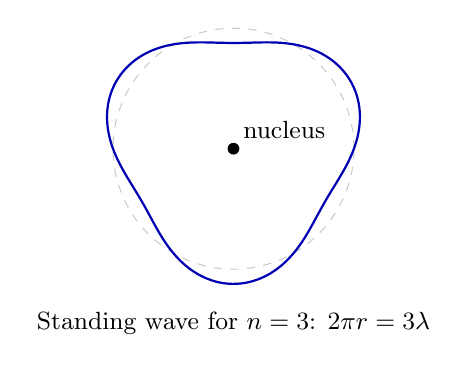
\begin{tikzpicture}[scale=0.85]
  % n=3 orbit: standing wave around circle
  \def\R{1.8}
  \draw[gray!40, dashed] (0,0) circle (\R);
  \draw[blue!70!black, thick, domain=0:360, samples=200]
    plot ({(\R + 0.22*sin(3*\x))*cos(\x)},
         {(\R + 0.22*sin(3*\x))*sin(\x)});
  \node[below] at (0,-2.3)
    {\small Standing wave for $n = 3$: $2\pi r = 3\lambda$};
  \fill (0,0) circle (2.5pt) node[above right]{\small nucleus};
\end{tikzpicture}
\end{center}

\medskip
\textbf{4. Experimental Verification}

\begin{enumerate}[label=(\roman*)]
    \item \textbf{Davisson--Germer Experiment (1927):} Electrons were diffracted
    by a nickel crystal, producing a diffraction pattern identical to that of
    X-rays. This conclusively proved the \textbf{wave nature of electrons}.

    \item \textbf{G.P. Thomson's Experiment (1927):} A beam of electrons passed
    through a thin gold foil produced concentric diffraction rings on a
    photographic plate, further confirming wave behaviour.
\end{enumerate}

\medskip
\textbf{5. Heisenberg's Uncertainty Principle --- A Consequence}

The wave--particle duality directly leads to Heisenberg's Uncertainty Principle:
it is impossible to simultaneously determine the exact position and momentum
of a particle:
\[
    \Delta x \cdot \Delta p \geq \frac{h}{4\pi}
\]
This is not a limitation of instruments, but a fundamental property of matter
arising from its wave nature.

\medskip
\textbf{6. Significance}

\begin{itemize}[itemsep=3pt]
    \item Wave--particle duality is the \textbf{cornerstone of quantum mechanics}.
    \item It led to the development of the \textbf{Schr\"{o}dinger wave equation},
    replacing Bohr's classical orbits with quantum mechanical \textbf{orbitals}
    (probability distributions).
    \item For macroscopic objects, $\lambda = h/mv$ is negligibly small, so wave
    nature is unobservable. For subatomic particles (electrons, protons), the
    wavelength is comparable to atomic dimensions, making wave behaviour significant.
\end{itemize}

\medskip
\textbf{Summary Table:}
\begin{center}
\begin{tabular}{lll}
\toprule
\textbf{Property} & \textbf{Particle Nature} & \textbf{Wave Nature} \\
\midrule
Evidence   & Photoelectric effect      & Electron diffraction \\
Described by & Momentum $p = mv$       & Wavelength $\lambda = h/p$ \\
Equation   & $E = mc^2$                & $\lambda = h/mv$ \\
Principle  & Newton's laws             & Schr\"{o}dinger equation \\
\bottomrule
\end{tabular}
\end{center}

\end{tcolorbox}


\item Group the species that are isoelectronic: Be$^{2+}$, F$^-$, Fe$^{2+}$, N$^{3-}$, He, S$^{2-}$, Co$^{3+}$, Ar. \mk{8}
\yr{CHEM 113 | 2011--12}

\begin{tcolorbox}[enhanced,breakable,ansbox,colback=cA!4,colframe=cA,boxrule=0.8pt,arc=5pt,title={\textbf{Answer}},fonttitle=\bfseries\color{white},colbacktitle=cA]
\textbf{Isoelectronic Species}

Isoelectronic species are atoms or ions that have the \textbf{same number of electrons}.

\medskip
\textbf{Step 1: Count the electrons in each species}

\begin{center}
\begin{tabular}{clcc}
\toprule
\textbf{Species} & \textbf{Atomic No.\ / Configuration} & \textbf{Charge} & \textbf{Electrons} \\
\midrule
He        & $Z = 2$  & 0    & 2  \\
Be$^{2+}$ & $Z = 4$  & $+2$ & 2  \\
\midrule
N$^{3-}$  & $Z = 7$  & $-3$ & 10 \\
F$^{-}$   & $Z = 9$  & $-1$ & 10 \\
\midrule
S$^{2-}$  & $Z = 16$ & $-2$ & 18 \\
Ar        & $Z = 18$ & 0    & 18 \\
\midrule
Fe$^{2+}$ & $Z = 26$ & $+2$ & 24 \\
Co$^{3+}$ & $Z = 27$ & $+3$ & 24 \\
\bottomrule
\end{tabular}
\end{center}

\medskip
\textbf{Step 2: Group the Isoelectronic Species}

\begin{enumerate}[label=(\roman*)]
    \item \textbf{2 electrons:}
    \[
        \text{He}, \quad \text{Be}^{2+}
    \]
    Both have the electron configuration $1s^2$.

    \item \textbf{10 electrons:}
    \[
        \text{N}^{3-}, \quad \text{F}^{-}
    \]
    Both have the electron configuration $1s^2\,2s^2\,2p^6$.

    \item \textbf{18 electrons:}
    \[
        \text{S}^{2-}, \quad \text{Ar}
    \]
    Both have the electron configuration $1s^2\,2s^2\,2p^6\,3s^2\,3p^6$.

    \item \textbf{24 electrons:}
    \[
        \text{Fe}^{2+}, \quad \text{Co}^{3+}
    \]
    Both have the electron configuration $[\text{Ar}]\,3d^6$.
\end{enumerate}

\end{tcolorbox}

\item Ionization energy is usually measured in the gaseous state. Why? \mk{7}
\yr{CHEM 113 | 2011--12}

\begin{tcolorbox}[enhanced,breakable,ansbox,colback=cA!4,colframe=cA,boxrule=0.8pt,arc=5pt,title={\textbf{Answer}},fonttitle=\bfseries\color{white},colbacktitle=cA]
\textbf{Why is Ionization Energy Measured in the Gaseous State?}

\medskip
\textbf{Definition:}
Ionization energy (IE) is the minimum energy required to remove the most loosely
bound electron from a neutral isolated atom:
\[
    \text{A}(g) \longrightarrow \text{A}^+(g) + e^- \qquad \Delta E = IE
\]

\medskip
\textbf{Reasons for Using the Gaseous State:}

\begin{enumerate}[label=(\roman*)]
    \item \textbf{Atoms are isolated and independent:}
    In the gaseous state, atoms are far apart from one another with negligible
    intermolecular forces. This ensures that the measured energy corresponds
    only to the \textbf{removal of an electron from a single, isolated atom},
    without any interference from neighbouring atoms or molecules.

    \item \textbf{Eliminates lattice energy contributions:}
    In the solid state, atoms are held together by strong \textbf{lattice forces}
    (in ionic/metallic solids) or intermolecular forces. Removing an electron
    from a solid would require overcoming both the ionization energy \textit{and}
    these lattice interactions, making it impossible to isolate the true IE.

    \item \textbf{Eliminates solvation energy contributions:}
    In the liquid or aqueous state, atoms/ions are surrounded by solvent
    molecules, contributing \textbf{solvation energy}. This would distort
    the measured value of IE since extra energy is involved in breaking
    solute--solvent interactions.

    \item \textbf{Gives a pure, intrinsic atomic property:}
    The gaseous state provides a \textbf{reference state} where the atom is in
    its standard, unperturbed condition. The IE measured is therefore a
    true \textbf{intrinsic property} of the atom, reflecting only the
    nuclear attraction on the outermost electron.

    \item \textbf{Allows meaningful comparison between elements:}
    Since all disturbing effects (lattice, solvation, intermolecular forces)
    are absent in the gas phase, ionization energies measured in this state
    can be \textbf{directly and fairly compared} across different elements
    in the periodic table.

    \item \textbf{Consistent with theoretical calculations:}
    Quantum mechanical models (Bohr model, Schr\"{o}dinger equation) calculate
    ionization energies for \textbf{isolated gaseous atoms}. Measuring IE in
    the gas phase ensures that experimental values match theoretical predictions
    without correction factors.
\end{enumerate}

\medskip
\textbf{Summary:}
\begin{center}
\begin{tabular}{lll}
\toprule
\textbf{State} & \textbf{Problem} & \textbf{Effect on IE} \\
\midrule
Solid  & Lattice energy present      & IE appears larger than true value \\
Liquid & Solvation energy present    & IE value gets distorted \\
Gas    & No external interactions    & True, intrinsic IE is measured \\
\bottomrule
\end{tabular}
\end{center}

\medskip
\textbf{Conclusion:}
The gaseous state is chosen because it eliminates all external energetic
contributions, ensuring that the measured ionization energy reflects
\textbf{only the electrostatic attraction between the nucleus and the
outermost electron} of an isolated atom.

\end{tcolorbox}

\item What are the limitations of Bohr's atomic theory? \mk{4}
\yr{CHEM 113 | 2011--12}

\begin{tcolorbox}[enhanced,breakable,ansbox,colback=cA!4,colframe=cA,boxrule=0.8pt,arc=5pt,title={\textbf{Answer}},fonttitle=\bfseries\color{white},colbacktitle=cA]
\textbf{Limitations of Bohr's Atomic Theory}

\begin{enumerate}[label=(\roman*)]
    \item \textbf{Fails for Multi-electron Atoms:}
    Bohr's model works only for \textbf{hydrogen-like species} (H, He$^+$,
    Li$^{2+}$, etc.). It fails completely for atoms with two or more electrons
    because it does not account for \textbf{electron--electron repulsions}.

    \item \textbf{Cannot Explain Fine Structure of Spectral Lines:}
    When hydrogen spectral lines are observed under high resolution or in the
    presence of a magnetic field, each line splits into several closely spaced
    lines (\textbf{Zeeman effect} and \textbf{Stark effect}). Bohr's theory
    cannot explain this fine and hyperfine splitting.

    \item \textbf{Violates Heisenberg's Uncertainty Principle:}
    Bohr assumed that electrons move in \textbf{fixed circular orbits} with
    precisely defined radius and velocity. This contradicts Heisenberg's
    Uncertainty Principle, which states that the position and momentum of an
    electron cannot be simultaneously determined with exactness:
    \[
        \Delta x \cdot \Delta p \geq \frac{h}{4\pi}
    \]

    \item \textbf{Does Not Account for Wave Nature of Electron:}
    Bohr treated the electron purely as a \textbf{classical particle}. It
    ignores the wave--particle duality of the electron established by
    de Broglie, which is fundamental to modern quantum mechanics.

\end{enumerate}

\end{tcolorbox}

\item State the general periodic trends in size of atomic radii. Arrange the following atoms in order of decreasing atomic radius: Na, Al, P, Cl, Mg. \mk{9}
\yr{CHEM 113 | 2011--12}

\begin{tcolorbox}[enhanced,breakable,ansbox,colback=cA!4,colframe=cA,boxrule=0.8pt,arc=5pt,title={\textbf{Answer}},fonttitle=\bfseries\color{white},colbacktitle=cA]
\textbf{Part 1: Periodic Trends in Atomic Radii}

\medskip
\textbf{Definition:}
Atomic radius is defined as \textbf{half the distance between the nuclei of two
identical adjacent atoms} in a molecule or crystal.

\medskip
\textbf{Trend 1: Across a Period (Left $\rightarrow$ Right)}

Atomic radius \textbf{decreases} across a period from left to right.

\begin{itemize}[itemsep=2pt]
    \item Moving across a period, the \textbf{number of protons increases}
    (higher nuclear charge $Z$), but electrons are added to the \textbf{same
    principal shell}.
    \item The increased nuclear charge pulls the electron cloud \textbf{closer
    to the nucleus}, reducing the atomic radius.
    \item Shielding effect remains approximately constant across a period.
\end{itemize}

\[
    \text{Atomic radius:}\quad \text{Na} > \text{Mg} > \text{Al} > \text{Si}
    > \text{P} > \text{Cl} > \text{Ar}
\]

\begin{center}
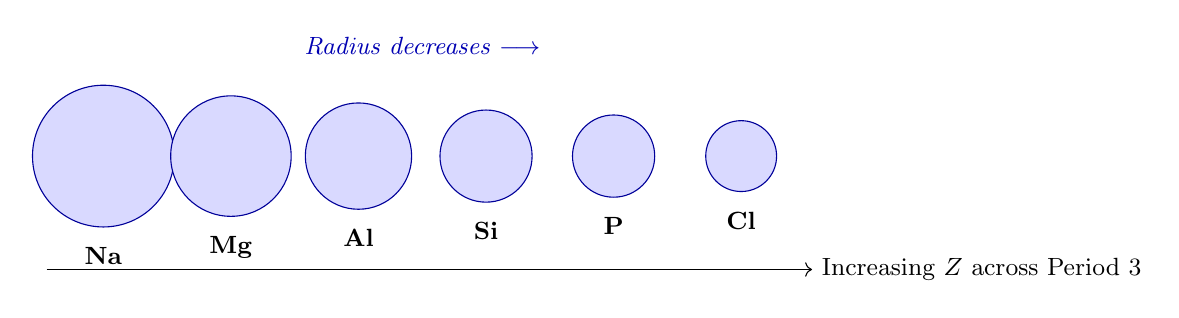
\begin{tikzpicture}[scale=0.9]
    \foreach \x/\el/\r in {
        0/Na/1.0, 1/Mg/0.85, 2/Al/0.75, 3/Si/0.65, 4/P/0.58, 5/Cl/0.50}{
        \draw[blue!60!black, fill=blue!15] (\x*1.8, 0) circle (\r);
        \node[below] at (\x*1.8, -\r-0.15) {\small\textbf{\el}};
    }
    \draw[->] (-0.8, -1.6) -- (10.0, -1.6)
        node[right]{\small Increasing $Z$ across Period 3};
    \node[left, font=\small] at (-0.8,-1.6) {};
    \node[above, font=\small\itshape, blue!70!black] at (4.5, 1.3)
        {Radius decreases $\longrightarrow$};
\end{tikzpicture}
\end{center}

\medskip
\textbf{Trend 2: Down a Group (Top $\rightarrow$ Bottom)}

Atomic radius \textbf{increases} down a group.

\begin{itemize}[itemsep=2pt]
    \item Moving down a group, each successive element has electrons in a
    \textbf{higher principal quantum shell} ($n$ increases).
    \item The outermost electrons are \textbf{farther from the nucleus}.
    \item Increased \textbf{shielding by inner electrons} reduces effective
    nuclear charge felt by the outermost electrons.
    \item Both effects cause the atomic radius to \textbf{increase}.
\end{itemize}

\[
    \text{Atomic radius:}\quad \text{Li} < \text{Na} < \text{K} < \text{Rb}
    < \text{Cs}
\]

\medskip
\textbf{Summary of Trends:}
\begin{center}
\begin{tabular}{lll}
\toprule
\textbf{Direction} & \textbf{Trend} & \textbf{Reason} \\
\midrule
Across a period (L $\to$ R) & Decreases & Increasing $Z$, same shell \\
Down a group (Top $\to$ Bottom) & Increases & New shell added, more shielding \\
\bottomrule
\end{tabular}
\end{center}

\medskip
\hrule
\medskip

\textbf{Part 2: Arrange Na, Al, P, Cl, Mg in Decreasing Atomic Radius}

\medskip
All five elements belong to \textbf{Period 3} of the periodic table:

\begin{center}
\begin{tabular}{clcc}
\toprule
\textbf{Element} & \textbf{Atomic No.} & \textbf{Period 3 Position}
& \textbf{Atomic Radius (pm)} \\
\midrule
Na & 11 & 1st & 186 \\
Mg & 12 & 2nd & 160 \\
Al & 13 & 3rd & 143 \\
P  & 15 & 5th & 110 \\
Cl & 17 & 7th & 99  \\
\bottomrule
\end{tabular}
\end{center}

Since all are in the same period, atomic radius \textbf{decreases with
increasing atomic number}. Therefore, the order of \textbf{decreasing
atomic radius} is:

\[
\boxed{\text{Na} > \text{Mg} > \text{Al} > \text{P} > \text{Cl}}
\]

\end{tcolorbox}

\item Derive an expression applying Bohr atom model for the calculation of wavelength of radiation obtained in the emission spectrum of hydrogen. \mk{10}
\yr{CHEM 101 | 2010--11}

\begin{tcolorbox}[enhanced,breakable,ansbox,colback=cA!4,colframe=cA,boxrule=0.8pt,arc=5pt,title={\textbf{Answer}},fonttitle=\bfseries\color{white},colbacktitle=cA]
\textbf{Derivation of Wavelength Expression Using Bohr's Atomic Model}

\medskip
\textbf{Bohr's Postulates (relevant):}
\begin{enumerate}[label=(\roman*)]
    \item Electrons revolve in fixed circular orbits without radiating energy.
    \item Energy is emitted or absorbed only when an electron transitions between orbits.
    \item The angular momentum of the electron is quantized:
    \[ m_e v r = \frac{nh}{2\pi} \]
\end{enumerate}

\medskip
\textbf{Step 1: Energy of an Electron in the $n$-th Orbit}

Balancing centripetal and electrostatic forces:
\[
\frac{m_e v^2}{r} = \frac{e^2}{4\pi\varepsilon_0 r^2}
\implies r = \frac{e^2}{4\pi\varepsilon_0 m_e v^2}
\]

From the quantization condition:
\[
v = \frac{nh}{2\pi m_e r}
\]

Solving simultaneously, the radius of the $n$-th orbit:
\[
r_n = \frac{n^2 h^2 \varepsilon_0}{\pi m_e e^2}
\]

The total energy (KE + PE) of the electron in the $n$-th orbit:
\[
E_n = -\frac{m_e e^4}{8\varepsilon_0^2 h^2} \cdot \frac{1}{n^2}
\]

\medskip
\textbf{Step 2: Energy of Emitted Photon}

When an electron transitions from a higher orbit $n_2$ to a lower orbit $n_1$ ($n_2 > n_1$), the energy of the emitted photon is:
\[
\Delta E = E_{n_2} - E_{n_1} = \frac{m_e e^4}{8\varepsilon_0^2 h^2}
\left(\frac{1}{n_1^2} - \frac{1}{n_2^2}\right)
\]

\medskip
\textbf{Step 3: Expression for Wavelength}

Since $\Delta E = h\nu = \dfrac{hc}{\lambda}$:
\[
\frac{hc}{\lambda} = \frac{m_e e^4}{8\varepsilon_0^2 h^2}
\left(\frac{1}{n_1^2} - \frac{1}{n_2^2}\right)
\]

\[
\boxed{\frac{1}{\lambda} = \frac{m_e e^4}{8\varepsilon_0^2 h^3 c}
\left(\frac{1}{n_1^2} - \frac{1}{n_2^2}\right)}
\]

\medskip
\textbf{Step 4: The Rydberg Constant}

The term $\dfrac{m_e e^4}{8\varepsilon_0^2 h^3 c}$ is the \textbf{Rydberg constant} $R_H$:
\[
R_H = \frac{m_e e^4}{8\varepsilon_0^2 h^3 c} = 1.097 \times 10^7 \, \text{m}^{-1}
\]

Thus the final expression becomes:
\[
\boxed{\frac{1}{\lambda} = R_H \left(\frac{1}{n_1^2} - \frac{1}{n_2^2}\right)}
\]

where $n_1 = 1, 2, 3, \ldots$ and $n_2 = n_1+1,\, n_1+2, \ldots$

\medskip
\textbf{Spectral Series of Hydrogen:}
\begin{center}
\begin{tabular}{llcc}
\toprule
\textbf{Series} & \textbf{Region} & $n_1$ & $n_2$ \\
\midrule
Lyman   & Ultraviolet  & 1 & 2, 3, 4, \ldots \\
Balmer  & Visible      & 2 & 3, 4, 5, \ldots \\
Paschen & Infrared     & 3 & 4, 5, 6, \ldots \\
Brackett & Infrared   & 4 & 5, 6, 7, \ldots \\
Pfund   & Far Infrared & 5 & 6, 7, 8, \ldots \\
\bottomrule
\end{tabular}
\end{center}

\end{tcolorbox}

\item What does Schr\"{o}dinger wave equation describe? Deduce the equation and comment on its solution. \mk{10}
\yr{CHEM 101 | 2010--11}

\begin{tcolorbox}[enhanced,breakable,ansbox,colback=cA!4,colframe=cA,boxrule=0.8pt,arc=5pt,title={\textbf{Answer}},fonttitle=\bfseries\color{white},colbacktitle=cA]
\textbf{The Schr\"{o}dinger Wave Equation}

\medskip
\textbf{Part 1: What Does It Describe?}

The Schr\"{o}dinger wave equation is the \textbf{fundamental equation of quantum
mechanics}. It describes:
\begin{itemize}[itemsep=3pt]
    \item The \textbf{wave-like behaviour} of a particle (e.g.\ an electron)
    in a given potential field.
    \item The \textbf{allowed energy states} (energy quantization) of a quantum
    mechanical system.
    \item The \textbf{wavefunction} $\psi$, which contains all information about
    the state of the particle.
    \item The \textbf{probability} of finding an electron at a given point in
    space, given by $|\psi|^2$ (Born interpretation).
\end{itemize}

It replaces Bohr's fixed circular orbits with \textbf{orbitals} --- three-dimensional
regions of space where the probability of finding an electron is highest.

\medskip
\hrule
\medskip

\textbf{Part 2: Deduction of the Schr\"{o}dinger Wave Equation}

\medskip
\textbf{Step 1: Classical Wave Equation}

A classical wave travelling in the $x$-direction is described by:
\[
    \psi(x) = A\sin\left(\frac{2\pi x}{\lambda}\right)
\]

Differentiating twice with respect to $x$:
\[
    \frac{d\psi}{dx} = A\cdot\frac{2\pi}{\lambda}\cos\left(\frac{2\pi x}{\lambda}\right)
\]
\[
    \frac{d^2\psi}{dx^2} = -A\left(\frac{2\pi}{\lambda}\right)^2
    \sin\left(\frac{2\pi x}{\lambda}\right) = -\frac{4\pi^2}{\lambda^2}\,\psi
\]

Rearranging:
\[
    \frac{d^2\psi}{dx^2} + \frac{4\pi^2}{\lambda^2}\,\psi = 0 \tag{1}
\]

\medskip
\textbf{Step 2: Substitute de Broglie Wavelength}

From de Broglie's relation:
\[
    \lambda = \frac{h}{mv} \implies \frac{1}{\lambda} = \frac{mv}{h}
    \implies \frac{4\pi^2}{\lambda^2} = \frac{4\pi^2 m^2 v^2}{h^2}
\]

Substituting into equation (1):
\[
    \frac{d^2\psi}{dx^2} + \frac{4\pi^2 m^2 v^2}{h^2}\,\psi = 0 \tag{2}
\]

\medskip
\textbf{Step 3: Express Kinetic Energy in Terms of Total Energy}

The total energy $E$ of the particle is the sum of kinetic energy (KE)
and potential energy (V):
\[
    E = \text{KE} + V = \frac{1}{2}mv^2 + V
\]
\[
    \text{KE} = \frac{1}{2}mv^2 = E - V
    \implies m^2v^2 = 2m(E-V)
\]

\medskip
\textbf{Step 4: Substituting into Equation (2)}

Replacing $m^2v^2$ with $2m(E-V)$:
\[
    \frac{d^2\psi}{dx^2} + \frac{4\pi^2}{h^2}\cdot 2m(E-V)\,\psi = 0
\]
\[
    \frac{d^2\psi}{dx^2} + \frac{8\pi^2 m}{h^2}(E-V)\,\psi = 0
\]

\medskip
\textbf{Step 5: Three-Dimensional Form}

Extending to three dimensions ($x, y, z$):
\[
    \frac{\partial^2\psi}{\partial x^2} +
    \frac{\partial^2\psi}{\partial y^2} +
    \frac{\partial^2\psi}{\partial z^2} +
    \frac{8\pi^2 m}{h^2}(E - V)\,\psi = 0
\]

Using the Laplacian operator
$\nabla^2 = \dfrac{\partial^2}{\partial x^2} +
             \dfrac{\partial^2}{\partial y^2} +
             \dfrac{\partial^2}{\partial z^2}$:

\[
    \boxed{\nabla^2\psi + \frac{8\pi^2 m}{h^2}(E - V)\,\psi = 0}
\]

This is the \textbf{time-independent Schr\"{o}dinger wave equation}.

Using $\hbar = \dfrac{h}{2\pi}$, it is equivalently written as:
\[
    -\frac{\hbar^2}{2m}\nabla^2\psi + V\psi = E\psi
    \quad\text{or}\quad \hat{H}\psi = E\psi
\]
where $\hat{H}$ is the \textbf{Hamiltonian operator}.

\medskip
\hrule
\medskip

\textbf{Part 3: Comments on the Solution}

\begin{enumerate}[label=(\roman*)]
    \item \textbf{The Wavefunction $\psi$:}
    The solution of the Schr\"{o}dinger equation gives the wavefunction $\psi$,
    which is a mathematical function of the coordinates of the electron
    $(x, y, z)$. By itself, $\psi$ has no direct physical meaning.

    \item \textbf{Physical Interpretation --- Born's Interpretation:}
    The square of the wavefunction, $|\psi|^2$, gives the
    \textbf{probability density} of finding the electron at a point in space.
    A large $|\psi|^2$ at a point means a high probability of finding the
    electron there.

    \item \textbf{Quantization of Energy:}
    Acceptable solutions exist only for \textbf{specific values of energy} $E$,
    called \textbf{eigenvalues}. This naturally explains the quantization of
    energy levels without any arbitrary assumption (unlike Bohr's model).

    \item \textbf{Quantum Numbers:}
    The solutions introduce three quantum numbers naturally:
    \begin{itemize}[itemsep=2pt]
        \item $n$ --- principal quantum number
        \item $l$ --- azimuthal quantum number
        \item $m_l$ --- magnetic quantum number
    \end{itemize}

    \item \textbf{Acceptable (Well-behaved) Wavefunctions:}
    Not all mathematical solutions are physically acceptable.
    A valid $\psi$ must be:
    \begin{itemize}[itemsep=2pt]
        \item \textbf{Single-valued} at every point
        \item \textbf{Continuous} and \textbf{finite} everywhere
        \item \textbf{Normalizable:} $\displaystyle\int_{-\infty}^{+\infty}
        |\psi|^2\,d\tau = 1$
    \end{itemize}

    \item \textbf{Orbitals:}
    Each acceptable solution $\psi_{n,l,m_l}$ describes an \textbf{atomic
    orbital} --- a three-dimensional probability distribution for the electron,
    replacing Bohr's classical circular orbits.
\end{enumerate}

\end{tcolorbox}

\item Mention the variations of the following properties of the elements within periods and groups in the periodic table and give reasons for these variations: (i) Oxidation power, (ii) Metallic character, (iii) Ionic radii, (iv) Reducing power, (v) Atomic size. \mk{7}
\yr{CHEM 101 | 2010--11}

\begin{tcolorbox}[enhanced,breakable,ansbox,colback=cA!4,colframe=cA,boxrule=0.8pt,arc=5pt,title={\textbf{Answer}},fonttitle=\bfseries\color{white},colbacktitle=cA]
\textbf{Periodic Variations of Properties in the Periodic Table}

\medskip

%% ── (i) Oxidation Power ──────────────────────────────────────────────
\textbf{(i) Oxidation Power}

\begin{itemize}[itemsep=2pt]
    \item \textbf{Across a period (L$\to$R):} Oxidation power \textbf{increases}.
    As nuclear charge increases across a period, the tendency to attract
    electrons (electronegativity) increases, so elements become stronger
    oxidizing agents.

    \item \textbf{Down a group (Top$\to$Bottom):} Oxidation power
    \textbf{decreases}. Atomic radius increases and shielding increases
    down the group, reducing the tendency to attract electrons.
    \[
        \text{e.g.,}\quad F_2 > Cl_2 > Br_2 > I_2
        \quad\text{(oxidizing power)}
    \]
\end{itemize}

\medskip

%% ── (ii) Metallic Character ──────────────────────────────────────────
\textbf{(ii) Metallic Character}

\begin{itemize}[itemsep=2pt]
    \item \textbf{Across a period (L$\to$R):} Metallic character
    \textbf{decreases}. Increasing nuclear charge makes it harder to lose
    electrons, so elements become less metallic and more non-metallic.

    \item \textbf{Down a group (Top$\to$Bottom):} Metallic character
    \textbf{increases}. Increased atomic radius and shielding reduce the
    effective nuclear charge on valence electrons, making them easier to
    lose.
    \[
        \text{e.g.,}\quad \text{Li} < \text{Na} < \text{K} < \text{Rb}
        \quad\text{(metallic character)}
    \]
\end{itemize}

\medskip

%% ── (iii) Ionic Radii ────────────────────────────────────────────────
\textbf{(iii) Ionic Radii}

\begin{itemize}[itemsep=2pt]
    \item \textbf{Cations} are always \textbf{smaller} than their parent
    atoms (loss of electrons reduces electron--electron repulsion, and
    nuclear charge pulls remaining electrons inward).

    \item \textbf{Anions} are always \textbf{larger} than their parent
    atoms (gain of electrons increases repulsion, expanding the electron
    cloud).

    \item \textbf{Across a period (L$\to$R):} For isoelectronic ions,
    ionic radius \textbf{decreases} with increasing nuclear charge.
    \[
        \text{e.g.,}\quad
        \text{N}^{3-} > \text{O}^{2-} > \text{F}^{-} > \text{Na}^{+}
        > \text{Mg}^{2+}
    \]

    \item \textbf{Down a group (Top$\to$Bottom):} Ionic radius
    \textbf{increases} as electrons occupy higher principal shells.
    \[
        \text{e.g.,}\quad
        \text{F}^- < \text{Cl}^- < \text{Br}^- < \text{I}^-
    \]
\end{itemize}

\medskip

%% ── (iv) Reducing Power ──────────────────────────────────────────────
\textbf{(iv) Reducing Power}

\begin{itemize}[itemsep=2pt]
    \item \textbf{Across a period (L$\to$R):} Reducing power
    \textbf{decreases}. Ionization energy increases across a period,
    making it harder for atoms to donate electrons and act as reducing
    agents.

    \item \textbf{Down a group (Top$\to$Bottom):} Reducing power
    \textbf{increases}. Ionization energy decreases down a group (larger
    atomic size, more shielding), making electron donation easier.
    \[
        \text{e.g.,}\quad
        \text{Li} < \text{Na} < \text{K} < \text{Rb} < \text{Cs}
        \quad\text{(reducing power)}
    \]
\end{itemize}

\medskip

%% ── (v) Atomic Size ──────────────────────────────────────────────────
\textbf{(v) Atomic Size}

\begin{itemize}[itemsep=2pt]
    \item \textbf{Across a period (L$\to$R):} Atomic size
    \textbf{decreases}. Nuclear charge $Z$ increases while electrons are
    added to the \textbf{same shell}, so the nucleus pulls the electron
    cloud inward more strongly.

    \item \textbf{Down a group (Top$\to$Bottom):} Atomic size
    \textbf{increases}. Each new period adds a new principal shell,
    placing valence electrons farther from the nucleus. Increased
    shielding by inner electrons further reduces the effective nuclear
    charge.
    \[
        \text{e.g.,}\quad
        \text{Li} < \text{Na} < \text{K} < \text{Rb} < \text{Cs}
        \quad\text{(atomic size)}
    \]
\end{itemize}

\medskip
\textbf{Summary Table:}
\begin{center}
\begin{tabular}{lcc}
\toprule
\textbf{Property} & \textbf{Across Period (L$\to$R)} &
\textbf{Down Group (Top$\to$Bottom)} \\
\midrule
Oxidation power  & Increases  & Decreases \\
Metallic character & Decreases & Increases \\
Ionic radii      & Decreases  & Increases \\
Reducing power   & Decreases  & Increases \\
Atomic size      & Decreases  & Increases \\
\bottomrule
\end{tabular}
\end{center}

\end{tcolorbox}

\item Calculate the magnitude of energy in erg of a quantum associated with light of wavelength 60.0 \AA. \mk{8}
\yr{CHEM 101 | 2010--11}

\begin{tcolorbox}[enhanced,breakable,ansbox,colback=cA!4,colframe=cA,boxrule=0.8pt,arc=5pt,title={\textbf{Answer}},fonttitle=\bfseries\color{white},colbacktitle=cA]
\textbf{Energy of a Quantum of Light}

\medskip
\textbf{Given:}
\begin{itemize}[itemsep=2pt]
    \item Wavelength: $\lambda = 60.0\,\text{\AA} = 60.0 \times 10^{-8}\,\text{cm}$
    \item Planck's constant: $h = 6.626 \times 10^{-27}\,\text{erg·s}$
    \item Speed of light: $c = 3.0 \times 10^{10}\,\text{cm·s}^{-1}$
\end{itemize}

\medskip
\textbf{Formula:}

The energy of a photon (quantum) is given by:
\[
    E = h\nu = \frac{hc}{\lambda}
\]

\medskip
\textbf{Calculation:}

\[
    E = \frac{hc}{\lambda}
    = \frac{6.626 \times 10^{-27}\,\text{erg·s}
            \times 3.0 \times 10^{10}\,\text{cm·s}^{-1}}
           {60.0 \times 10^{-8}\,\text{cm}}
\]

\[
    E = \frac{6.626 \times 3.0}{60.0}
        \times 10^{-27+10+8}\,\text{erg}
\]

\[
    E = \frac{19.878}{60.0} \times 10^{-9}\,\text{erg}
\]

\[
    E = 0.3313 \times 10^{-9}\,\text{erg}
\]

\[
    \boxed{E = 3.313 \times 10^{-10}\,\text{erg}}
\]

\medskip
\textbf{Note:}
This wavelength ($60.0\,\text{\AA} = 6.0\,\text{nm}$) lies in the
\textbf{extreme ultraviolet (EUV)} region of the electromagnetic spectrum.
The high energy of this quantum ($3.313 \times 10^{-10}$ erg) is consistent
with the short wavelength, as energy and wavelength are inversely related:
\[
    E \propto \frac{1}{\lambda}
\]

\end{tcolorbox}

\item What is quantum theory of radiation? Discuss photoelectric effect in relation to quantization of energy. \mk{10}
\yr{CHEM 101 | 2009--10}

\begin{tcolorbox}[enhanced,breakable,ansbox,colback=cA!4,colframe=cA,boxrule=0.8pt,arc=5pt,title={\textbf{Answer}},fonttitle=\bfseries\color{white},colbacktitle=cA]
\textbf{Quantum Theory of Radiation and Photoelectric Effect}

\medskip
\textbf{Part 1: Quantum Theory of Radiation (Planck, 1900)}

Classical physics assumed that energy is emitted or absorbed
\textbf{continuously} in any amount. This failed to explain
blackbody radiation (the ``ultraviolet catastrophe'').

Max Planck proposed the \textbf{Quantum Theory of Radiation} based on
the following postulates:

\begin{enumerate}[label=(\roman*)]
    \item Energy is not emitted or absorbed continuously, but in
    \textbf{discrete packets} called \textbf{quanta} (singular: quantum).

    \item The energy of each quantum is directly proportional to the
    frequency $\nu$ of the radiation:
    \[
        E = h\nu
    \]
    where $h = 6.626 \times 10^{-34}$ J$\cdot$s is \textbf{Planck's constant}.

    \item A body can emit or absorb energy only in \textbf{whole number
    multiples} of $h\nu$:
    \[
        E = nh\nu \qquad (n = 1,\, 2,\, 3,\, \ldots)
    \]

    \item Energy is \textbf{quantized} --- it cannot take arbitrary values,
    only discrete allowed values.
\end{enumerate}

This was a revolutionary departure from classical physics and laid the
foundation of \textbf{modern quantum mechanics}.

\medskip
\hrule
\medskip

\textbf{Part 2: Photoelectric Effect}

\medskip
\textbf{Definition:}
The \textbf{photoelectric effect} is the phenomenon in which
\textbf{electrons are ejected from the surface of a metal} when light
of sufficient frequency is incident upon it.

\medskip
\textbf{Experimental Observations:}

\begin{enumerate}[label=(\roman*)]
    \item Electrons are emitted \textbf{only if the frequency} of incident
    light exceeds a minimum value called the \textbf{threshold frequency}
    $\nu_0$, regardless of the intensity of light.

    \item \textbf{Below} $\nu_0$, no electrons are emitted even if the
    light is very intense.

    \item The \textbf{kinetic energy} of emitted electrons increases with
    increasing frequency, but is \textbf{independent of intensity}.

    \item Increasing the \textbf{intensity} of light increases the
    \textbf{number} of emitted electrons, not their kinetic energy.

    \item Electron emission is \textbf{instantaneous} --- there is no
    time delay.
\end{enumerate}

\medskip
\textbf{Failure of Classical Theory:}

Classical wave theory predicted that:
\begin{itemize}[itemsep=2pt]
    \item Any frequency of light should eventually eject electrons if
    intensity is high enough.
    \item There should be a time delay before emission.
\end{itemize}
Both predictions \textbf{contradicted} experimental results.

\medskip
\textbf{Einstein's Quantum Explanation (1905):}

Einstein extended Planck's quantum theory and proposed that light
consists of \textbf{photons} --- discrete packets of energy. Each
photon carries energy:
\[
    E = h\nu
\]

When a photon strikes a metal surface:
\begin{itemize}[itemsep=2pt]
    \item A part of the photon energy is used to overcome the
    \textbf{work function} $\phi = h\nu_0$ (the minimum energy needed
    to eject an electron).
    \item The remaining energy appears as the \textbf{kinetic energy}
    of the ejected electron.
\end{itemize}

This gives \textbf{Einstein's photoelectric equation}:
\[
    \boxed{h\nu = h\nu_0 + \frac{1}{2}m_e v^2}
\]
\[
    \frac{1}{2}m_e v^2 = h\nu - h\nu_0 = h(\nu - \nu_0)
\]

where:
\begin{itemize}[itemsep=2pt]
    \item $h\nu$ = energy of incident photon
    \item $h\nu_0 = \phi$ = work function of the metal
    \item $\dfrac{1}{2}m_e v^2$ = kinetic energy of emitted electron
\end{itemize}

\medskip
\textbf{Diagram:}

\begin{center}
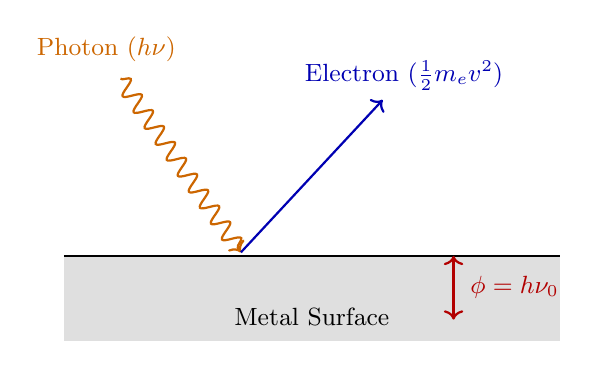
\begin{tikzpicture}[scale=0.9]
    % Metal surface
    \fill[gray!25] (0,-1.2) rectangle (7,0);
    \draw[thick] (0,0) -- (7,0);
    \node[below] at (3.5,-0.6) {\small Metal Surface};

    % Incident photon
    \draw[->, thick, orange!80!black, decorate,
          decoration={snake, amplitude=3pt, segment length=7pt}]
        (0.8, 2.5) -- (2.5, 0.05);
    \node[above, orange!80!black] at (0.6, 2.6) {\small Photon ($h\nu$)};

    % Ejected electron
    \draw[->, thick, blue!70!black] (2.5, 0.05) -- (4.5, 2.2);
    \node[above, blue!70!black] at (4.8, 2.2)
        {\small Electron ($\frac{1}{2}m_ev^2$)};

    % Work function label
    \draw[<->, red!70!black, thick] (5.5, 0) -- (5.5, -0.9);
    \node[right, red!70!black, font=\small] at (5.6, -0.45)
        {$\phi = h\nu_0$};
\end{tikzpicture}
\end{center}

\medskip
\textbf{Relation to Quantization of Energy:}

\begin{enumerate}[label=(\roman*)]
    \item The photoelectric effect provides \textbf{direct experimental
    proof} that light energy is quantized into photons of energy $h\nu$.

    \item A single photon interacts with a single electron in an
    \textbf{all-or-nothing} fashion --- the electron is either ejected
    or not, depending on whether $h\nu \geq h\nu_0$.

    \item The \textbf{instantaneous} nature of emission confirms that
    energy is delivered in discrete packets, not spread continuously
    over time as a wave.

    \item The \textbf{threshold frequency} $\nu_0$ is direct evidence
    of energy quantization: only photons with $E = h\nu \geq \phi$ can
    eject electrons.
\end{enumerate}

\medskip
\textbf{Summary Table:}
\begin{center}
\begin{tabular}{lll}
\toprule
\textbf{Observation} & \textbf{Classical Prediction} &
\textbf{Quantum Explanation} \\
\midrule
Threshold frequency & Not explained & $E = h\nu \geq \phi$ \\
KE depends on $\nu$ & Not explained & $\text{KE} = h(\nu - \nu_0)$ \\
Intensity $\to$ number & Not explained & More photons $=$ more electrons \\
Instantaneous emission & Time delay expected & One photon ejects one electron \\
\bottomrule
\end{tabular}
\end{center}

\end{tcolorbox}

\item What are the limitations of Bohr's atomic theory and how are they overcome? \mk{10}
\yr{CHEM 101 | 2009--10}

\begin{tcolorbox}[enhanced,breakable,ansbox,colback=cA!4,colframe=cA,boxrule=0.8pt,arc=5pt,title={\textbf{Answer}},fonttitle=\bfseries\color{white},colbacktitle=cA]
\textbf{Limitations of Bohr's Atomic Theory and How They Are Overcome}

\medskip
\textbf{Part 1: Limitations of Bohr's Atomic Theory}

\begin{enumerate}[label=(\roman*)]
    \item \textbf{Fails for Multi-electron Atoms:}
    Bohr's model works only for \textbf{hydrogen-like species}
    (H, He$^+$, Li$^{2+}$, etc.). It completely fails for atoms
    with two or more electrons because it does not account for
    \textbf{electron--electron repulsion}, which significantly
    affects energy levels.

    \item \textbf{Cannot Explain Fine Structure of Spectral Lines:}
    Under high resolution, each spectral line of hydrogen splits
    into several closely spaced lines. Bohr's theory predicts only
    single lines and cannot account for this
    \textbf{fine and hyperfine splitting}.

    \item \textbf{Cannot Explain Zeeman and Stark Effects:}
    When atoms are placed in an external \textbf{magnetic field}
    (Zeeman effect) or \textbf{electric field} (Stark effect),
    spectral lines split further. Bohr's model has no mechanism
    to explain this splitting.

    \item \textbf{Violates Heisenberg's Uncertainty Principle:}
    Bohr assumed electrons move in \textbf{fixed circular orbits}
    with precisely defined positions and velocities simultaneously.
    This directly contradicts Heisenberg's Uncertainty Principle:
    \[
        \Delta x \cdot \Delta p \geq \frac{h}{4\pi}
    \]

    \item \textbf{Does Not Account for Wave Nature of Electron:}
    Bohr treated the electron purely as a \textbf{classical
    particle}, ignoring de Broglie's wave--particle duality.
    It does not explain why only certain orbits are stable.

    \item \textbf{Cannot Explain Relative Intensities of
    Spectral Lines:}
    Bohr's model predicts the \textbf{positions} of spectral
    lines but cannot predict why some lines are more intense
    than others.

    \item \textbf{Restricted to Circular Orbits:}
    Bohr assumed only \textbf{circular orbits}. Sommerfeld
    extended this to elliptical orbits, but even then the
    model remained fundamentally inadequate for multi-electron
    systems.

    \item \textbf{Cannot Explain Chemical Bonding:}
    Bohr's model provides no satisfactory explanation for
    \textbf{how atoms form bonds} to make molecules, since it
    treats each atom in isolation.
\end{enumerate}

\medskip
\hrule
\medskip

\textbf{Part 2: How the Limitations Are Overcome}

\begin{enumerate}[label=(\roman*)]
    \item \textbf{Quantum Mechanical Model (Schr\"{o}dinger, 1926):}
    Schr\"{o}dinger replaced Bohr's classical circular orbits with
    \textbf{orbitals} by solving the wave equation:
    \[
        \nabla^2\psi + \frac{8\pi^2 m}{h^2}(E - V)\psi = 0
    \]
    This model works for \textbf{all atoms}, including multi-electron
    systems, by incorporating electron--electron repulsions through
    approximate methods (e.g.\ Hartree--Fock).

    \item \textbf{Introduction of Four Quantum Numbers:}
    The quantum mechanical model introduces \textbf{four quantum
    numbers} to fully describe the state of an electron:
    \begin{center}
    \begin{tabular}{cll}
    \toprule
    \textbf{Quantum No.} & \textbf{Symbol} & \textbf{Describes} \\
    \midrule
    Principal       & $n$   & Energy level / shell size \\
    Azimuthal       & $l$   & Shape of orbital (subshell) \\
    Magnetic        & $m_l$ & Orientation in space \\
    Spin            & $m_s$ & Electron spin ($+\frac{1}{2}$ or $-\frac{1}{2}$) \\
    \bottomrule
    \end{tabular}
    \end{center}
    The \textbf{spin quantum number} $m_s$ explains the fine structure
    of spectral lines and the Zeeman effect.

    \item \textbf{Heisenberg's Uncertainty Principle Incorporated:}
    The quantum mechanical model abandons the concept of fixed orbits.
    Instead, $|\psi|^2$ gives the \textbf{probability density} of
    finding an electron, fully consistent with the uncertainty
    principle.

    \item \textbf{de Broglie's Wave Nature Incorporated:}
    The Schr\"{o}dinger equation is itself a \textbf{wave equation},
    naturally incorporating the wave nature of the electron. Stable
    orbits correspond to \textbf{standing waves}:
    \[
        2\pi r = n\lambda \implies m_e vr = \frac{nh}{2\pi}
    \]

    \item \textbf{Zeeman and Stark Effects Explained:}
    By including the magnetic quantum number $m_l$ and spin quantum
    number $m_s$, quantum mechanics successfully explains the splitting
    of spectral lines in external magnetic and electric fields.

    \item \textbf{Relative Intensities Explained:}
    Quantum mechanics introduces \textbf{selection rules} and
    \textbf{transition probabilities} that determine which transitions
    are allowed and how intense the corresponding spectral lines are.

    \item \textbf{Chemical Bonding Explained:}
    The quantum mechanical model forms the basis of
    \textbf{molecular orbital theory} and \textbf{valence bond theory},
    which successfully explain how atoms combine to form molecules
    through overlap of orbitals.
\end{enumerate}

\medskip
\textbf{Summary Table:}
\begin{center}
\begin{tabular}{ll}
\toprule
\textbf{Limitation of Bohr's Model} & \textbf{How Overcome} \\
\midrule
Fails for multi-electron atoms   & Schr\"{o}dinger equation + approximations \\
No fine structure explanation    & Spin quantum number $m_s$ \\
Violates uncertainty principle   & Probability-based orbital model \\
Ignores wave nature of electron  & de Broglie + wave equation \\
No Zeeman/Stark effect           & Magnetic \& spin quantum numbers \\
Cannot explain bonding           & MO theory \& VB theory \\
\bottomrule
\end{tabular}
\end{center}

\end{tcolorbox}

\item Justify the stability of a nucleus of an atom. \mk{8}
\yr{CHEM 101 | 2009--10}

\begin{tcolorbox}[enhanced,breakable,ansbox,colback=cA!4,colframe=cA,boxrule=0.8pt,arc=5pt,title={\textbf{Answer}},fonttitle=\bfseries\color{white},colbacktitle=cA]
\textbf{Stability of a Nucleus of an Atom}

\medskip
\textbf{1. Composition of the Nucleus}

The nucleus of an atom consists of \textbf{protons} (positively charged)
and \textbf{neutrons} (electrically neutral), collectively called
\textbf{nucleons}. Since protons are positively charged and confined in
an extremely small volume ($\sim 10^{-15}$ m), they experience enormous
\textbf{electrostatic repulsion}. Yet the nucleus remains stable ---
this requires explanation.

\medskip
\textbf{2. Nuclear Force (Strong Force)}

The primary reason for nuclear stability is the \textbf{strong nuclear
force}, which acts between all nucleons (proton--proton,
neutron--neutron, proton--neutron). It is much stronger than
electrostatic repulsion (about $100\times$ stronger at short range),
is \textbf{short-range} (effective only up to $\sim 10^{-15}$ m), and
is \textbf{charge independent}. As long as the strong nuclear force
overcomes electrostatic repulsion, the nucleus remains stable.

\medskip
\textbf{3. Neutron-to-Proton Ratio ($n/p$ Ratio)}

The ratio of neutrons to protons is a key factor in nuclear stability.
For light nuclei ($Z \leq 20$), stable nuclei have $n/p \approx 1$
(e.g.\ $^{12}_{6}$C has 6 protons and 6 neutrons). For heavier nuclei
($Z > 20$), more neutrons are needed to dilute proton--proton
repulsion, so $n/p > 1$ (e.g.\ $^{208}_{82}$Pb has $n/p \approx 1.54$).
If $n/p$ is too high or too low, the nucleus becomes unstable and
undergoes radioactive decay.

\medskip
\textbf{4. Nuclear Binding Energy}

\textbf{Binding energy} is the energy required to completely separate
all nucleons in a nucleus. It arises from the \textbf{mass defect}
$\Delta m$, the difference between the mass of the nucleus and the
sum of masses of its individual nucleons:
\begin{equation*}
    \Delta m = Z\,m_p + N\,m_n - m_{\text{nucleus}}
\end{equation*}

By Einstein's mass--energy relation:
\begin{equation*}
    E_b = \Delta m \cdot c^2
\end{equation*}

The \textbf{binding energy per nucleon} ($E_b/A$) measures nuclear
stability. Higher $E_b/A$ means a more stable nucleus. The maximum
$E_b/A \approx 8.8$ MeV occurs near $^{56}_{26}$Fe (iron), making it
the most stable nucleus. Nuclei lighter or heavier than iron undergo
\textbf{fusion} or \textbf{fission} respectively to reach greater
stability.

\medskip
\textbf{5. Magic Numbers}

Certain nuclei are exceptionally stable when the number of protons
or neutrons equals a \textbf{magic number}: 2, 8, 20, 28, 50, 82, 126.
These correspond to completely filled nuclear shells, providing extra
stability. Examples include $^{4}_{2}$He (doubly magic),
$^{16}_{8}$O (doubly magic), and $^{208}_{82}$Pb (doubly magic).

\medskip
\textbf{6. Even--Odd Rule}

The stability of a nucleus also depends on whether the number of
protons and neutrons is even or odd:

\begin{center}
\begin{tabular}{cccc}
\toprule
\textbf{Protons} & \textbf{Neutrons} &
\textbf{Stable nuclides} & \textbf{Stability} \\
\midrule
Even & Even & $\sim$157 & Most stable \\
Even & Odd  & $\sim$53  & Moderately stable \\
Odd  & Even & $\sim$50  & Moderately stable \\
Odd  & Odd  & $\sim$5   & Least stable \\
\bottomrule
\end{tabular}
\end{center}

Even numbers of both protons and neutrons allow nucleons to pair up
with opposite spins, lowering energy and enhancing stability.

\medskip
\textbf{Summary:}
Nuclear stability is determined by a combination of strong nuclear
force, optimal $n/p$ ratio, high binding energy per nucleon,
magic numbers, and even--even nucleon pairing.

\end{tcolorbox}

\item What is periodic law? How many periods and groups are there in a periodic table? Why are the periods not equal? \mk{8}
\yr{CHEM 101 | 2009--10}

\begin{tcolorbox}[enhanced,breakable,ansbox,colback=cA!4,colframe=cA,boxrule=0.8pt,arc=5pt,title={\textbf{Answer}},fonttitle=\bfseries\color{white},colbacktitle=cA]
\textbf{Periodic Law, Periods, Groups and Their Inequality}

\medskip
\textbf{Part 1: Periodic Law}

The \textbf{Modern Periodic Law} (Moseley, 1913) states:

\begin{center}
\textit{``The physical and chemical properties of elements are periodic
functions of their \textbf{atomic numbers}.''}
\end{center}

This was a refinement of \textbf{Mendeleev's Periodic Law} (1869),
which stated that properties are periodic functions of
\textbf{atomic masses}. Moseley corrected this by showing that
\textbf{atomic number} (number of protons), not atomic mass, is the
fundamental property that determines the position and properties
of an element.

\medskip
\textbf{Part 2: Periods in the Periodic Table}

A \textbf{period} is a horizontal row in the periodic table. There are
\textbf{7 periods} in total:

\begin{center}
\begin{tabular}{cccp{6cm}}
\toprule
\textbf{Period} & \textbf{Elements} & \textbf{No.\ of Elements}
& \textbf{Highest Shell Filled} \\
\midrule
1 & H to He       & 2  & $n = 1$ (1s) \\
2 & Li to Ne      & 8  & $n = 2$ (2s, 2p) \\
3 & Na to Ar      & 8  & $n = 3$ (3s, 3p) \\
4 & K to Kr       & 18 & $n = 4$ (4s, 3d, 4p) \\
5 & Rb to Xe      & 18 & $n = 5$ (5s, 4d, 5p) \\
6 & Cs to Rn      & 32 & $n = 6$ (6s, 4f, 5d, 6p) \\
7 & Fr to Og      & 32 & $n = 7$ (7s, 5f, 6d, 7p) \\
\bottomrule
\end{tabular}
\end{center}

\medskip
\textbf{Part 3: Groups in the Periodic Table}

A \textbf{group} is a vertical column in the periodic table. There are
\textbf{18 groups} in the modern periodic table (IUPAC), numbered
1 to 18. Elements in the same group have the same
\textbf{valence electron configuration} and hence similar chemical
properties. For example, Group 1 (alkali metals) all have one valence
electron and are highly reactive.

\medskip
\textbf{Part 4: Why Are the Periods Not Equal in Length?}

The periods are unequal in length because the \textbf{number of
elements in each period depends on the number of electrons that can
be accommodated in the subshells} of the corresponding principal
quantum shell.

The maximum number of electrons in a shell is given by $2n^2$, and
the subshells available determine the number of elements per period.
The key reasoning is:

\begin{enumerate}[label=(\roman*)]
    \item \textbf{Period 1 (2 elements):}
    Only the $1s$ subshell is filled. It holds a maximum of
    2 electrons:
    \begin{equation*}
        1s^2 \quad \Rightarrow \quad 2 \text{ elements}
    \end{equation*}

    \item \textbf{Periods 2 and 3 (8 elements each):}
    The $s$ and $p$ subshells of $n = 2$ and $n = 3$ are filled.
    The $d$ subshell of $n = 3$ is not filled until period 4:
    \begin{equation*}
        ns^2\,np^6 \quad \Rightarrow \quad 2 + 6 = 8 \text{ elements}
    \end{equation*}

    \item \textbf{Periods 4 and 5 (18 elements each):}
    The $s$, $d$, and $p$ subshells are filled. The $3d$ subshell
    (10 electrons) is included in period 4:
    \begin{equation*}
        ns^2\,(n{-}1)d^{10}\,np^6
        \quad \Rightarrow \quad 2 + 10 + 6 = 18 \text{ elements}
    \end{equation*}

    \item \textbf{Periods 6 and 7 (32 elements each):}
    The $s$, $f$, $d$, and $p$ subshells are all filled. The $4f$
    subshell (14 electrons) is included:
    \begin{equation*}
        ns^2\,(n{-}2)f^{14}\,(n{-}1)d^{10}\,np^6
        \quad \Rightarrow \quad 2 + 14 + 10 + 6 = 32 \text{ elements}
    \end{equation*}
\end{enumerate}

\medskip
\textbf{Summary:}
\begin{center}
\begin{tabular}{ccc}
\toprule
\textbf{Subshells Filled} & \textbf{Electrons} & \textbf{Period Length} \\
\midrule
$s$             & 2            & 2  \\
$s + p$         & $2+6$        & 8  \\
$s + d + p$     & $2+10+6$     & 18 \\
$s + f + d + p$ & $2+14+10+6$  & 32 \\
\bottomrule
\end{tabular}
\end{center}

The periods are not equal because different principal shells contain
different numbers of subshells, and each subshell has a different
capacity for electrons ($s$: 2, $p$: 6, $d$: 10, $f$: 14).

\end{tcolorbox}

\item How would you conceive the idea of having an electron cloud around the nucleus of an atom? How is it experimentally proved that the electron has wave nature? \mk{11}
\yr{CHEM 101 | 2009--10}

\begin{tcolorbox}[enhanced,breakable,ansbox,colback=cA!4,colframe=cA,boxrule=0.8pt,arc=5pt,title={\textbf{Answer}},fonttitle=\bfseries\color{white},colbacktitle=cA]
\textbf{Electron Cloud and Experimental Proof of Wave Nature of Electron}

\medskip
\textbf{Part 1: The Concept of Electron Cloud}

\medskip
\textbf{Background --- Failure of Bohr's Orbit:}

Bohr's model assumed electrons move in \textbf{fixed circular orbits}
with a definite position and velocity at every instant. However,
\textbf{Heisenberg's Uncertainty Principle} states:
\begin{equation*}
    \Delta x \cdot \Delta p \geq \frac{h}{4\pi}
\end{equation*}
It is fundamentally impossible to know the exact position and momentum
of an electron simultaneously. Therefore, the concept of a fixed orbit
is physically meaningless.

\medskip
\textbf{Quantum Mechanical Picture --- The Electron Cloud:}

In the quantum mechanical model, the electron is not confined to a
fixed orbit. Instead, its behaviour is described by the
\textbf{wavefunction} $\psi$, obtained by solving the
Schr\"{o}dinger equation:
\begin{equation*}
    \nabla^2\psi + \frac{8\pi^2 m}{h^2}(E - V)\psi = 0
\end{equation*}

The physical meaning of $\psi$ is given by \textbf{Born's
interpretation}: the quantity $|\psi|^2$ at any point in space
represents the \textbf{probability density} of finding the electron
at that point. This leads to the concept of the \textbf{electron cloud}:

\begin{itemize}[itemsep=3pt]
    \item The electron does not follow a fixed path. Instead, it
    occupies a \textbf{three-dimensional region} around the nucleus
    called an \textbf{orbital}.

    \item The \textbf{density of the cloud} at any point is
    proportional to $|\psi|^2$ --- regions of high density indicate
    high probability of finding the electron, and regions of low
    density indicate low probability.

    \item The electron cloud is \textbf{not a physical rotating cloud};
    it is a \textbf{probability map} showing where the electron is most
    likely to be found.

    \item For the hydrogen atom ground state ($1s$ orbital), the
    electron cloud is \textbf{spherically symmetric} and most dense
    near the nucleus, becoming diffuse further away.
\end{itemize}

\begin{center}
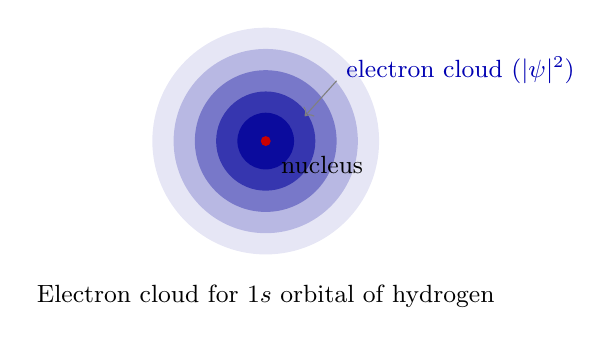
\begin{tikzpicture}[scale=0.9]
    % Electron cloud: concentric shaded circles
    \foreach \r/\op in {1.6/10, 1.3/20, 1.0/35, 0.7/55, 0.4/80}{
        \fill[blue!60!black, opacity=\op/100] (0,0) circle (\r);
    }
    \fill[red!80!black] (0,0) circle (0.07);
    \node[below right, font=\small] at (0.08,-0.08) {nucleus};
    \node[right, font=\small, blue!70!black] at (1.0, 1.0)
        {electron cloud ($|\psi|^2$)};
    \draw[->, gray] (1.0, 0.85) -- (0.55, 0.35);
    \node[below, font=\small] at (0,-1.9)
        {\small Electron cloud for $1s$ orbital of hydrogen};
\end{tikzpicture}
\end{center}

\medskip
\hrule
\medskip

\textbf{Part 2: Experimental Proof of Wave Nature of Electron}

\medskip
\textbf{Theoretical Basis --- de Broglie's Hypothesis (1924):}

de Broglie proposed that every moving particle has an associated
wavelength:
\begin{equation*}
    \lambda = \frac{h}{mv} = \frac{h}{p}
\end{equation*}
This predicted that electrons, being particles, should also exhibit
\textbf{wave behaviour} such as diffraction and interference.

\medskip
\textbf{Experiment 1: Davisson--Germer Experiment (1927)}

\begin{itemize}[itemsep=3pt]
    \item A beam of electrons was directed at a \textbf{nickel crystal}
    surface at various angles.
    \item The crystal acted as a \textbf{diffraction grating} (the
    inter-atomic spacing $\sim 10^{-10}$ m is comparable to the
    de Broglie wavelength of electrons).
    \item A \textbf{diffraction pattern} was observed --- electrons
    were scattered at specific angles with maximum and minimum
    intensities, exactly like X-rays (which are known waves).
    \item The measured wavelength matched the de Broglie prediction:
    \begin{equation*}
        \lambda = \frac{h}{mv}
    \end{equation*}
    \item This was \textbf{direct experimental proof} that electrons
    have wave nature.
\end{itemize}

\begin{center}
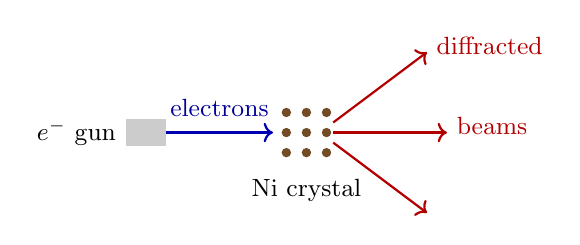
\begin{tikzpicture}[scale=0.85]
    % Electron gun
    \fill[gray!40] (0,0.2) rectangle (0.6,-0.2);
    \node[left, font=\small] at (0,0) {$e^-$ gun};

    % Electron beam
    \draw[->, thick, blue!70!black] (0.6,0) -- (2.2,0);
    \node[above, font=\small, blue!60!black] at (1.4, 0.1)
        {electrons};

    % Nickel crystal
    \foreach \y in {-0.3, 0, 0.3}{
        \foreach \x in {2.4, 2.7, 3.0}{
            \fill[brown!60!black] (\x,\y) circle (0.07);
        }
    }
    \node[below, font=\small] at (2.7,-0.55) {Ni crystal};

    % Diffracted beams
    \draw[->, thick, red!70!black]  (3.1, 0.15) -- (4.5,  1.2);
    \draw[->, thick, red!70!black]  (3.1, 0.00) -- (4.8,  0.0);
    \draw[->, thick, red!70!black]  (3.1,-0.15) -- (4.5, -1.2);
    \node[right, font=\small, red!70!black] at (4.5, 1.3)
        {diffracted};
    \node[right, font=\small, red!70!black] at (4.8, 0.1)
        {beams};
\end{tikzpicture}
\end{center}

\medskip
\textbf{Experiment 2: G.P. Thomson's Experiment (1927)}

\begin{itemize}[itemsep=3pt]
    \item A beam of high-energy electrons was passed through a
    \textbf{thin gold foil}.
    \item On a photographic plate placed behind the foil,
    \textbf{concentric circular diffraction rings} were observed ---
    identical to those produced by X-rays passing through a
    crystalline material.
    \item This pattern is only possible if electrons behave as
    \textbf{waves} and undergo diffraction through the regular
    atomic planes of the gold crystal.
    \item G.P.\ Thomson was awarded the \textbf{Nobel Prize} in 1937
    for this discovery (shared with Davisson).
\end{itemize}

\medskip
\textbf{Significance:}

\begin{enumerate}[label=(\roman*)]
    \item Both experiments confirmed \textbf{de Broglie's hypothesis}
    that matter has wave nature.
    \item The wave nature of the electron is the physical basis for the
    \textbf{electron cloud model} and the Schr\"{o}dinger equation.
    \item It established \textbf{wave--particle duality} as a
    fundamental property of all matter.
\end{enumerate}

\end{tcolorbox}

\item Deduce an equation by which the propagation of electron wave in space can be described. How can the solutions of the equation be used to describe the different shapes of orbitals? \mk{12}
\yr{CHEM 101 | 2009--10}

\begin{tcolorbox}[enhanced,breakable,ansbox,colback=cA!4,colframe=cA,boxrule=0.8pt,arc=5pt,title={\textbf{Answer}},fonttitle=\bfseries\color{white},colbacktitle=cA]
\textbf{Schr\"{o}dinger Wave Equation and Shapes of Orbitals}

\medskip
\textbf{Part 1: Deduction of the Schr\"{o}dinger Wave Equation}

\medskip
\textbf{Step 1: Classical Wave Equation}

A wave travelling in the $x$-direction is mathematically described by:
\begin{equation*}
    \psi(x) = A\sin\left(\frac{2\pi x}{\lambda}\right)
\end{equation*}

Differentiating twice with respect to $x$:
\begin{equation*}
    \frac{d\psi}{dx} = A \cdot \frac{2\pi}{\lambda}
    \cos\left(\frac{2\pi x}{\lambda}\right)
\end{equation*}
\begin{equation*}
    \frac{d^2\psi}{dx^2} = -A\left(\frac{2\pi}{\lambda}\right)^2
    \sin\left(\frac{2\pi x}{\lambda}\right)
    = -\frac{4\pi^2}{\lambda^2}\,\psi
\end{equation*}

Rearranging:
\begin{equation*}
    \frac{d^2\psi}{dx^2} + \frac{4\pi^2}{\lambda^2}\,\psi = 0
    \tag{1}
\end{equation*}

\medskip
\textbf{Step 2: Introduce de Broglie Wavelength}

From de Broglie's relation $\lambda = \dfrac{h}{mv}$:
\begin{equation*}
    \frac{1}{\lambda^2} = \frac{m^2v^2}{h^2}
    \quad\Rightarrow\quad
    \frac{4\pi^2}{\lambda^2} = \frac{4\pi^2 m^2 v^2}{h^2}
\end{equation*}

Substituting into equation (1):
\begin{equation*}
    \frac{d^2\psi}{dx^2} + \frac{4\pi^2 m^2 v^2}{h^2}\,\psi = 0
    \tag{2}
\end{equation*}

\medskip
\textbf{Step 3: Express Using Total Energy}

Total energy $E$ = Kinetic energy + Potential energy $V$:
\begin{equation*}
    E = \frac{1}{2}mv^2 + V
    \quad\Rightarrow\quad
    \frac{1}{2}mv^2 = E - V
    \quad\Rightarrow\quad
    m^2v^2 = 2m(E - V)
\end{equation*}

Substituting into equation (2):
\begin{equation*}
    \frac{d^2\psi}{dx^2} + \frac{8\pi^2 m}{h^2}(E - V)\,\psi = 0
\end{equation*}

\medskip
\textbf{Step 4: Extend to Three Dimensions}

Extending to three dimensions $(x, y, z)$:
\begin{equation*}
    \frac{\partial^2\psi}{\partial x^2} +
    \frac{\partial^2\psi}{\partial y^2} +
    \frac{\partial^2\psi}{\partial z^2} +
    \frac{8\pi^2 m}{h^2}(E - V)\,\psi = 0
\end{equation*}

Using the Laplacian operator
$\nabla^2 = \dfrac{\partial^2}{\partial x^2} +
\dfrac{\partial^2}{\partial y^2} +
\dfrac{\partial^2}{\partial z^2}$,
the \textbf{Schr\"{o}dinger wave equation} is:

\begin{equation*}
    \boxed{\nabla^2\psi + \frac{8\pi^2 m}{h^2}(E - V)\,\psi = 0}
\end{equation*}

Using $\hbar = \dfrac{h}{2\pi}$, this is equivalently written as:
\begin{equation*}
    \hat{H}\psi = E\psi
    \qquad\text{where}\qquad
    \hat{H} = -\frac{\hbar^2}{2m}\nabla^2 + V
\end{equation*}
is the \textbf{Hamiltonian operator}.

\medskip
\hrule
\medskip

\textbf{Part 2: Solutions and Shapes of Orbitals}

\medskip
\textbf{Nature of Solutions:}

Solving the Schr\"{o}dinger equation in spherical polar coordinates
$(r, \theta, \phi)$ gives solutions of the form:
\begin{equation*}
    \psi_{n,l,m_l}(r,\theta,\phi)
    = R_{n,l}(r) \cdot Y_{l,m_l}(\theta,\phi)
\end{equation*}

where:
\begin{itemize}[itemsep=2pt]
    \item $R_{n,l}(r)$ is the \textbf{radial wavefunction} ---
    describes how $\psi$ varies with distance $r$ from the nucleus.
    \item $Y_{l,m_l}(\theta,\phi)$ is the \textbf{angular wavefunction}
    --- describes the \textbf{shape and orientation} of the orbital.
\end{itemize}

Each solution is characterized by three quantum numbers:

\begin{center}
\begin{tabular}{cll}
\toprule
\textbf{Quantum Number} & \textbf{Symbol} & \textbf{Determines} \\
\midrule
Principal    & $n = 1, 2, 3\ldots$         & Size and energy of orbital \\
Azimuthal    & $l = 0, 1, \ldots, n-1$     & Shape of orbital \\
Magnetic     & $m_l = -l, \ldots, 0, \ldots, +l$ & Orientation in space \\
\bottomrule
\end{tabular}
\end{center}

\medskip
\textbf{Shapes of Orbitals from Solutions:}

\begin{enumerate}[label=(\roman*)]

    \item \textbf{$s$ Orbitals ($l = 0$):}
    The angular wavefunction $Y_{0,0}$ is a constant, independent of
    $\theta$ and $\phi$. Therefore, $|\psi|^2$ is the same in all
    directions --- the orbital is \textbf{perfectly spherical}.
    For each value of $n$, there is one $s$ orbital. As $n$ increases,
    the sphere becomes larger and contains $(n-1)$ radial nodes.

    \begin{center}
    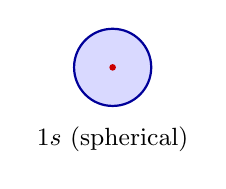
\begin{tikzpicture}[scale=0.7]
        \fill[blue!15] (0,0) circle (0.7);
        \draw[blue!60!black, thick] (0,0) circle (0.7);
        \fill[red!80!black] (0,0) circle (0.06);
        \node[below, font=\small] at (0,-0.9) {$1s$ (spherical)};
    \end{tikzpicture}
    \end{center}

    \item \textbf{$p$ Orbitals ($l = 1$):}
    There are three $p$ orbitals ($m_l = -1, 0, +1$), namely
    $p_x$, $p_y$, and $p_z$. The angular wavefunction gives a
    \textbf{dumbbell (figure-eight) shape} with two lobes on
    opposite sides of the nucleus along the $x$, $y$, or $z$ axis.
    There is a \textbf{nodal plane} passing through the nucleus where
    $\psi = 0$.

    \begin{center}
    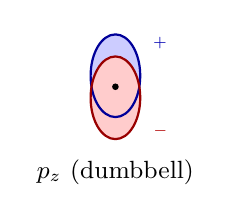
\begin{tikzpicture}[scale=0.7]
        % p_z orbital: two lobes along y-axis
        \fill[blue!20]  (0, 0.2) ellipse (0.45 and 0.75);
        \fill[red!20]   (0,-0.2) ellipse (0.45 and 0.75);
        \draw[blue!60!black, thick]  (0, 0.2) ellipse (0.45 and 0.75);
        \draw[red!60!black,  thick]  (0,-0.2) ellipse (0.45 and 0.75);
        \fill[black] (0,0) circle (0.06);
        \node[right, font=\tiny, blue!70!black] at (0.5,  0.8) {$+$};
        \node[right, font=\tiny, red!70!black]  at (0.5, -0.8) {$-$};
        \node[below, font=\small] at (0,-1.15) {$p_z$ (dumbbell)};
    \end{tikzpicture}
    \end{center}

    \item \textbf{$d$ Orbitals ($l = 2$):}
    There are five $d$ orbitals ($m_l = -2,-1,0,+1,+2$). Four of
    them ($d_{xy}$, $d_{xz}$, $d_{yz}$, $d_{x^2-y^2}$) have a
    \textbf{four-leaf clover (double dumbbell) shape} with four
    lobes. The fifth ($d_{z^2}$) has two lobes along the $z$-axis
    with a \textbf{doughnut-shaped ring} in the $xy$-plane.

    \item \textbf{$f$ Orbitals ($l = 3$):}
    There are seven $f$ orbitals ($m_l = -3$ to $+3$) with
    complex \textbf{multi-lobed shapes}. They are involved in
    the chemistry of lanthanides and actinides.

\end{enumerate}

\medskip
\textbf{Nodes in Orbitals:}

The number of nodes (regions where $\psi = 0$) also follows from
the solutions:
\begin{center}
\begin{tabular}{lcc}
\toprule
\textbf{Type} & \textbf{Number} & \textbf{Depends on} \\
\midrule
Radial nodes   & $n - l - 1$ & Principal \& azimuthal QN \\
Angular nodes  & $l$         & Azimuthal QN \\
Total nodes    & $n - 1$     & Principal QN only \\
\bottomrule
\end{tabular}
\end{center}

\medskip
\textbf{Summary:}
The solutions $\psi_{n,l,m_l}$ of the Schr\"{o}dinger equation
directly yield the \textbf{shapes, sizes, orientations,} and
\textbf{energies} of atomic orbitals through the three quantum
numbers $n$, $l$, and $m_l$. The probability density $|\psi|^2$
gives the \textbf{electron cloud distribution}, which defines the
physical shape of each orbital.

\end{tcolorbox}

\item What are the transition elements and which periods of the periodic table do they belong to? Discuss the important properties of transition elements. \mk{7}
\yr{CHEM 101 | 2008--09}

\begin{tcolorbox}[enhanced,breakable,ansbox,colback=cA!4,colframe=cA,boxrule=0.8pt,arc=5pt,title={\textbf{Answer}},fonttitle=\bfseries\color{white},colbacktitle=cA]
\textbf{Transition Elements: Definition, Periods and Properties}

\medskip
\textbf{Part 1: Definition of Transition Elements}

Transition elements are defined as those elements in which the
\textbf{$d$ subshell is partially filled} either in the ground
state of the atom or in any of their commonly occurring ions.
They are also called \textbf{$d$-block elements}.

Formally, they are elements with the general electronic
configuration:
\begin{equation*}
    (n-1)d^{1-10}\; ns^{1-2}
\end{equation*}

\textbf{Note:} Zn, Cd, and Hg are sometimes excluded from the
strict definition because their $d$ subshell is completely
filled ($d^{10}$) in both ground state and common ions.

\medskip
\textbf{Part 2: Periods of the Periodic Table}

Transition elements occupy \textbf{Groups 3--12} and are found
in \textbf{Periods 4, 5, 6, and 7} of the periodic table,
forming four transition series:

\begin{center}
\begin{tabular}{clll}
\toprule
\textbf{Series} & \textbf{Period} & \textbf{Elements}
& \textbf{Configuration} \\
\midrule
1st (3d) & Period 4 & Sc ($Z=21$) to Zn ($Z=30$)
& $[Ar]\,3d^{1-10}\,4s^{1-2}$ \\
2nd (4d) & Period 5 & Y ($Z=39$) to Cd ($Z=48$)
& $[Kr]\,4d^{1-10}\,5s^{1-2}$ \\
3rd (5d) & Period 6 & La, Hf ($Z=72$) to Hg ($Z=80$)
& $[Xe]\,4f^{14}\,5d^{1-10}\,6s^{1-2}$ \\
4th (6d) & Period 7 & Ac, Rf ($Z=104$) to Cn ($Z=112$)
& $[Rn]\,5f^{14}\,6d^{1-10}\,7s^{1-2}$ \\
\bottomrule
\end{tabular}
\end{center}

\medskip
\hrule
\medskip

\textbf{Part 3: Important Properties of Transition Elements}

\begin{enumerate}[label=(\roman*)]

    \item \textbf{Variable Oxidation States:}
    Transition metals exhibit \textbf{multiple oxidation states}
    because both $(n-1)d$ and $ns$ electrons can participate in
    bonding. For example:
    \begin{equation*}
        \text{Mn: } +2,\,+3,\,+4,\,+6,\,+7
        \qquad
        \text{Fe: } +2,\,+3
        \qquad
        \text{Cr: } +2,\,+3,\,+6
    \end{equation*}

    \item \textbf{Formation of Coloured Compounds:}
    Most transition metal compounds are \textbf{coloured} because
    electrons in lower $d$ orbitals absorb visible light and are
    excited to higher $d$ orbitals (\textbf{$d$--$d$ transitions}).
    The complementary colour is observed. For example,
    CuSO$_4$ is blue, KMnO$_4$ is purple, and K$_2$Cr$_2$O$_7$
    is orange. Ions with $d^0$ (Sc$^{3+}$) or $d^{10}$ (Zn$^{2+}$)
    are colourless as $d$--$d$ transitions are not possible.

    \item \textbf{Magnetic Properties:}
    Transition metal compounds are often \textbf{paramagnetic}
    due to the presence of unpaired $d$ electrons. The magnetic
    moment is:
    \begin{equation*}
        \mu = \sqrt{n(n+2)}\;\text{ B.M.}
    \end{equation*}
    where $n$ is the number of unpaired electrons. Compounds
    with no unpaired electrons are \textbf{diamagnetic}.

    \item \textbf{Formation of Complex Compounds:}
    Transition metals readily form \textbf{coordination complexes}
    with ligands due to their small ionic size, high charge
    density, and available empty $d$ orbitals to accept lone
    pairs. Examples: $[\text{Fe(CN)}_6]^{3-}$,
    $[\text{Cu(NH}_3)_4]^{2+}$.

    \item \textbf{Catalytic Properties:}
    Transition metals are excellent \textbf{catalysts} due to
    their variable oxidation states and ability to adsorb
    reactants on their surfaces. Examples: Fe in the Haber
    process, V$_2$O$_5$ in the Contact process, Pt in catalytic
    converters.

    \item \textbf{High Melting and Boiling Points:}
    Transition metals have \textbf{high melting points} because
    both $s$ and $d$ electrons participate in strong metallic
    bonding. Tungsten (W) has the highest melting point of all
    metals (3422$^\circ$C).

    \item \textbf{Formation of Alloys:}
    Transition metals readily form \textbf{alloys} with each
    other due to similar atomic radii. Alloys are harder and
    more corrosion resistant than pure metals. Examples: steel
    (Fe $+$ C), brass (Cu $+$ Zn), nichrome (Ni $+$ Cr).

\end{enumerate}

\medskip
\textbf{Summary Table:}
\begin{center}
\begin{tabular}{ll}
\toprule
\textbf{Property} & \textbf{Reason} \\
\midrule
Variable oxidation states & $d$ and $s$ electrons both participate \\
Coloured compounds        & $d$--$d$ electronic transitions \\
Paramagnetism             & Unpaired $d$ electrons \\
Complex formation         & Empty $d$ orbitals, high charge density \\
Catalytic activity        & Variable valency, surface adsorption \\
High melting points       & Strong metallic bonding via $d$ electrons \\
\bottomrule
\end{tabular}
\end{center}

\end{tcolorbox}

\item What are noble gases? Discuss the important physical and chemical properties of noble gases. \mk{7}
\yr{CHEM 101 | 2008--09}

\begin{tcolorbox}[enhanced,breakable,ansbox,colback=cA!4,colframe=cA,boxrule=0.8pt,arc=5pt,title={\textbf{Answer}},fonttitle=\bfseries\color{white},colbacktitle=cA]
\textbf{Noble Gases: Definition and Properties}

\medskip
\textbf{Part 1: What are Noble Gases?}

Noble gases are the elements of \textbf{Group 18} (Group 0) of
the periodic table. They are also called \textbf{inert gases} or
\textbf{rare gases}. The six noble gases are:

\begin{center}
\begin{tabular}{clcc}
\toprule
\textbf{Symbol} & \textbf{Name} & \textbf{Atomic No.}
& \textbf{Configuration} \\
\midrule
He & Helium   & 2  & $1s^2$ \\
Ne & Neon     & 10 & $[He]\,2s^2\,2p^6$ \\
Ar & Argon    & 18 & $[Ne]\,3s^2\,3p^6$ \\
Kr & Krypton  & 36 & $[Ar]\,3d^{10}\,4s^2\,4p^6$ \\
Xe & Xenon    & 54 & $[Kr]\,4d^{10}\,5s^2\,5p^6$ \\
Rn & Radon    & 86 & $[Xe]\,4f^{14}\,5d^{10}\,6s^2\,6p^6$ \\
\bottomrule
\end{tabular}
\end{center}

Their outermost shell is \textbf{completely filled} ($ns^2np^6$,
except He which has $1s^2$), giving them exceptional stability
and very low chemical reactivity. This stable configuration is
called the \textbf{octet configuration} (or duplet for He).

\medskip
\hrule
\medskip

\textbf{Part 2: Physical Properties of Noble Gases}

\begin{enumerate}[label=(\roman*)]

    \item \textbf{State and Appearance:}
    All noble gases are \textbf{colourless, odourless, and
    tasteless} monoatomic gases under normal conditions. They
    exist as \textbf{single atoms} (monoatomic) because they
    have no tendency to form diatomic molecules.

    \item \textbf{Low Boiling and Melting Points:}
    Noble gases have \textbf{very low boiling and melting points}
    because the only intermolecular forces present are weak
    \textbf{London dispersion (van der Waals) forces}. These
    increase down the group as atomic size and polarizability
    increase:
    \begin{equation*}
        \text{B.P.:}\quad
        \text{He} < \text{Ne} < \text{Ar} < \text{Kr}
        < \text{Xe} < \text{Rn}
    \end{equation*}
    Helium has the \textbf{lowest boiling point} of any substance
    ($-269^\circ$C).

    \item \textbf{Low Density:}
    Noble gases have \textbf{very low densities} compared to
    other gases due to their low atomic masses (except Rn).
    Helium is the second lightest gas after hydrogen.

    \item \textbf{Low Solubility in Water:}
    Noble gases have \textbf{low but measurable solubility} in
    water, which increases down the group with increasing atomic
    size and polarizability.

    \item \textbf{Non-conductors:}
    In their normal state, noble gases are
    \textbf{non-conductors} of electricity. However, under high
    voltage, they \textbf{glow with characteristic colours}
    (used in neon signs): Ne (red-orange), Ar (blue-violet),
    Kr (pale violet), Xe (blue).

    \item \textbf{Monoatomic and Ideal Gas Behaviour:}
    Noble gases behave nearly as \textbf{ideal gases} because
    of negligible intermolecular interactions. Their $C_p/C_v
    = 5/3$, which is the theoretical value for a monoatomic
    ideal gas.

\end{enumerate}

\medskip
\hrule
\medskip

\textbf{Part 3: Chemical Properties of Noble Gases}

\begin{enumerate}[label=(\roman*)]

    \item \textbf{General Inertness:}
    Noble gases are \textbf{chemically very inert} due to their
    completely filled valence shells. They have:
    \begin{itemize}[itemsep=2pt]
        \item \textbf{Zero electron affinity} --- no tendency to
        gain electrons.
        \item \textbf{Very high ionization energies} --- very
        difficult to remove electrons.
        \item \textbf{No unpaired electrons} --- cannot form
        covalent bonds easily.
    \end{itemize}

    \item \textbf{Ionization Energy:}
    Noble gases have the \textbf{highest ionization energies}
    in their respective periods, decreasing down the group:
    \begin{equation*}
        IE:\quad \text{He} > \text{Ne} > \text{Ar}
        > \text{Kr} > \text{Xe} > \text{Rn}
    \end{equation*}

    \item \textbf{Compounds of Noble Gases:}
    Although generally inert, heavier noble gases (Kr, Xe, Rn)
    can form compounds under special conditions because their
    outer electrons are more loosely held (larger atomic radius,
    lower ionization energy). Important examples include:
    \begin{itemize}[itemsep=2pt]
        \item \textbf{Xenon compounds:}
        XeF$_2$, XeF$_4$, XeF$_6$, XeO$_3$, XeOF$_4$
        (first synthesized by Bartlett, 1962).
        \item \textbf{Krypton compounds:}
        KrF$_2$ (unstable at room temperature).
        \item \textbf{Radon compounds:}
        RnF$_2$ (radioactive, difficult to study).
    \end{itemize}
    He, Ne, and Ar form \textbf{no stable chemical compounds}
    under any known conditions.

    \item \textbf{Clathrate Compounds:}
    Noble gases can be \textbf{physically trapped} inside
    cavities of other molecules (e.g.\ ice, hydroquinone)
    to form \textbf{clathrates} or cage compounds. These are
    not true chemical compounds as no covalent bonds are formed.
    Example: Ar, Kr, Xe clathrates with water.

    \item \textbf{Reactivity Trend Down the Group:}
    Chemical reactivity \textbf{increases down the group}:
    \begin{equation*}
        \text{He} \approx \text{Ne} \approx \text{Ar}
        < \text{Kr} < \text{Xe} < \text{Rn}
    \end{equation*}
    This is because larger atoms have more polarizable electron
    clouds and lower ionization energies, making electron
    donation easier.

\end{enumerate}

\medskip
\textbf{Summary Table:}
\begin{center}
\begin{tabular}{ll}
\toprule
\textbf{Property} & \textbf{Reason} \\
\midrule
Chemical inertness      & Completely filled valence shell \\
Low boiling points      & Only weak van der Waals forces \\
High ionization energy  & Stable $ns^2np^6$ configuration \\
Xe forms compounds      & Large size, low IE, polarizable \\
He/Ne form no compounds & Very high IE, small size \\
\bottomrule
\end{tabular}
\end{center}

\end{tcolorbox}

\item Discuss the quantum theory of radiation. How is Planck's hypothesis for radiation of energy related to the spectral properties of an atom described by Bohr? \mk{13}
\yr{CHEM 101 | 2008--09}

\begin{tcolorbox}[enhanced,breakable,ansbox,colback=cA!4,colframe=cA,boxrule=0.8pt,arc=5pt,title={\textbf{Answer}},fonttitle=\bfseries\color{white},colbacktitle=cA]
\textbf{Quantum Theory of Radiation and Its Relation to Bohr's
Spectral Theory}

\medskip
\textbf{Part 1: Quantum Theory of Radiation (Planck, 1900)}

\medskip
\textbf{Background --- Failure of Classical Theory:}

Classical physics (Rayleigh--Jeans law) assumed that a
\textbf{blackbody} emits radiation continuously at all
frequencies with energy proportional to temperature. This
predicted that intensity should increase indefinitely at
high frequencies (ultraviolet region) --- a catastrophic
failure known as the \textbf{``ultraviolet catastrophe''},
which completely contradicted experimental observations.

\medskip
\textbf{Planck's Postulates:}

To resolve this, Max Planck (1900) proposed the
\textbf{Quantum Theory of Radiation} based on the following
postulates:

\begin{enumerate}[label=(\roman*)]
    \item A heated body does not emit or absorb energy
    \textbf{continuously}, but in \textbf{discrete packets}
    called \textbf{quanta} (singular: quantum). Each quantum
    is an indivisible unit of energy.

    \item The energy of each quantum is directly proportional
    to the \textbf{frequency} $\nu$ of the radiation:
    \begin{equation*}
        E = h\nu
    \end{equation*}
    where $h = 6.626 \times 10^{-34}$ J$\cdot$s is
    \textbf{Planck's constant}. Since $\nu = c/\lambda$:
    \begin{equation*}
        E = \frac{hc}{\lambda}
    \end{equation*}

    \item A body can emit or absorb energy only in
    \textbf{whole number multiples} of $h\nu$:
    \begin{equation*}
        E = nh\nu \qquad (n = 1,\, 2,\, 3,\, \ldots)
    \end{equation*}
    Energy is therefore \textbf{quantized} --- it cannot
    take arbitrary values, only specific discrete values.

    \item At \textbf{low frequencies}, the quantized
    description merges with classical theory
    (\textbf{Bohr's correspondence principle}).
\end{enumerate}

\medskip
\textbf{Significance of Planck's Theory:}

\begin{itemize}[itemsep=2pt]
    \item It successfully explained the observed
    \textbf{blackbody radiation spectrum}.
    \item It introduced the revolutionary idea that energy
    is \textbf{not continuous} but comes in discrete packets.
    \item It laid the foundation of \textbf{modern quantum
    mechanics}.
    \item Einstein extended it to explain the
    \textbf{photoelectric effect} (1905), proposing that
    light itself consists of photons of energy $h\nu$.
\end{itemize}

\medskip
\hrule
\medskip

\textbf{Part 2: Bohr's Atomic Model and Spectral Properties}

\medskip
Bohr (1913) applied Planck's quantum hypothesis directly
to the hydrogen atom. His model rests on the following
key ideas:

\begin{enumerate}[label=(\roman*)]
    \item Electrons revolve in \textbf{fixed quantized orbits}
    without emitting energy (stationary states).

    \item Angular momentum is quantized:
    \begin{equation*}
        m_e vr = \frac{nh}{2\pi}
    \end{equation*}

    \item Energy is emitted or absorbed as a photon
    \textbf{only during transitions} between orbits:
    \begin{equation*}
        \Delta E = E_{n_2} - E_{n_1} = h\nu
    \end{equation*}
\end{enumerate}

The total energy of the electron in the $n$-th orbit is:
\begin{equation*}
    E_n = -\frac{m_e e^4}{8\varepsilon_0^2 h^2}
    \cdot \frac{1}{n^2}
\end{equation*}

\medskip
\hrule
\medskip

\textbf{Part 3: Relation Between Planck's Hypothesis and
Bohr's Spectral Theory}

The connection between Planck's quantum hypothesis and
Bohr's description of atomic spectra is \textbf{deep and
direct}. The key links are:

\begin{enumerate}[label=(\roman*)]

    \item \textbf{Quantization of Energy Levels:}
    Bohr adopted Planck's idea that energy is quantized and
    applied it to electron orbits. Just as Planck quantized
    the energy of oscillators as $E = nh\nu$, Bohr quantized
    the \textbf{angular momentum} of electrons:
    \begin{equation*}
        m_e vr = \frac{nh}{2\pi}
    \end{equation*}
    This leads naturally to \textbf{discrete energy levels}
    $E_n \propto -1/n^2$, meaning only specific energies
    are allowed for the electron.

    \item \textbf{Energy of Emitted Photon:}
    When an electron transitions from level $n_2$ to $n_1$
    ($n_2 > n_1$), the energy difference is released as a
    \textbf{photon} --- directly using Planck's relation
    $E = h\nu$:
    \begin{equation*}
        \Delta E = E_{n_2} - E_{n_1}
        = \frac{m_e e^4}{8\varepsilon_0^2 h^2}
        \left(\frac{1}{n_1^2} - \frac{1}{n_2^2}\right)
        = h\nu
    \end{equation*}

    \item \textbf{Derivation of the Rydberg Equation:}
    Since $h\nu = hc/\lambda$, dividing both sides by $hc$:
    \begin{equation*}
        \frac{1}{\lambda}
        = \frac{m_e e^4}{8\varepsilon_0^2 h^3 c}
        \left(\frac{1}{n_1^2} - \frac{1}{n_2^2}\right)
        = R_H\left(\frac{1}{n_1^2} - \frac{1}{n_2^2}\right)
    \end{equation*}
    where $R_H = 1.097 \times 10^7\,\text{m}^{-1}$ is the
    \textbf{Rydberg constant}. This equation predicts the
    exact positions of all spectral lines of hydrogen.

    \item \textbf{Explanation of Line Spectra:}
    Classical theory predicted a \textbf{continuous spectrum}
    from atoms. Planck's quantization, as incorporated by
    Bohr, explains why atoms emit only \textbf{discrete
    spectral lines} --- because only specific energy
    transitions $\Delta E = h\nu$ are allowed between
    quantized levels.

    \item \textbf{Spectral Series of Hydrogen:}
    Different values of $n_1$ and $n_2$ in Bohr's equation
    give rise to different spectral series, all derivable
    using Planck's $E = h\nu$:
    \begin{center}
    \begin{tabular}{llcc}
    \toprule
    \textbf{Series} & \textbf{Region} & $n_1$ & $n_2$ \\
    \midrule
    Lyman    & Ultraviolet  & 1 & 2, 3, 4\ldots \\
    Balmer   & Visible      & 2 & 3, 4, 5\ldots \\
    Paschen  & Infrared     & 3 & 4, 5, 6\ldots \\
    Brackett & Far Infrared & 4 & 5, 6, 7\ldots \\
    Pfund    & Far Infrared & 5 & 6, 7, 8\ldots \\
    \bottomrule
    \end{tabular}
    \end{center}

    \item \textbf{Ionization Energy from Planck's Relation:}
    The ionization energy of hydrogen is obtained by setting
    $n_1 = 1$ and $n_2 = \infty$:
    \begin{equation*}
        IE = h\nu_{\text{max}}
        = \frac{m_e e^4}{8\varepsilon_0^2 h^2}
        = 13.6\,\text{eV}
    \end{equation*}
    This matches experimental values exactly, confirming
    that Planck's quantization is built into Bohr's model.

\end{enumerate}

\medskip
\textbf{Summary Table:}
\begin{center}
\begin{tabular}{ll}
\toprule
\textbf{Planck's Contribution} & \textbf{Bohr's Application} \\
\midrule
$E = h\nu$ (energy quantized)    & Quantized electron energy levels \\
Energy in discrete packets       & Only specific orbits allowed \\
Photon emitted: $E = h\nu$       & Spectral line at frequency $\nu$ \\
$\nu \propto \Delta E$           & Rydberg equation for $\lambda$ \\
No continuous energy emission    & Discrete line spectrum explained \\
\bottomrule
\end{tabular}
\end{center}

\medskip
\textbf{Conclusion:}
Planck's quantum hypothesis is the \textbf{direct foundation}
of Bohr's spectral theory. Bohr used $E = h\nu$ to connect
the energy difference between quantized atomic levels to the
frequency of emitted radiation, thereby explaining the origin,
position, and series of all spectral lines of hydrogen with
remarkable accuracy.

\end{tcolorbox}

\item What are the limitations of Bohr's atomic structure? How was the structure modified by Sommerfeld? \mk{10}
\yr{CHEM 101 | 2008--09}

\begin{tcolorbox}[enhanced,breakable,ansbox,colback=cA!4,colframe=cA,boxrule=0.8pt,arc=5pt,title={\textbf{Answer}},fonttitle=\bfseries\color{white},colbacktitle=cA]
\textbf{Limitations of Bohr's Model and Sommerfeld's Modification}

\medskip
\textbf{Part 1: Limitations of Bohr's Atomic Model}

\begin{enumerate}[label=(\roman*)]

    \item \textbf{Fails for Multi-electron Atoms:}
    Bohr's model works only for \textbf{hydrogen and hydrogen-like
    species} (He$^+$, Li$^{2+}$, etc.). It completely fails for
    atoms with two or more electrons because it does not account
    for \textbf{electron--electron repulsions}, which
    significantly alter the energy levels.

    \item \textbf{Cannot Explain Fine Structure of Spectral Lines:}
    Under high-resolution spectroscopy, each spectral line of
    hydrogen is found to consist of \textbf{several closely
    spaced lines} (fine structure). Bohr's model predicts only
    single lines for each transition and cannot explain this
    splitting.

    \item \textbf{Cannot Explain Zeeman and Stark Effects:}
    When atoms are placed in an external \textbf{magnetic field}
    (Zeeman effect) or \textbf{electric field} (Stark effect),
    spectral lines split into multiple components. Bohr's model
    has no mechanism to account for this splitting.

    \item \textbf{Violates Heisenberg's Uncertainty Principle:}
    Bohr assigned both a \textbf{definite position} (radius $r_n$)
    and a \textbf{definite velocity} to electrons simultaneously.
    This directly violates Heisenberg's Uncertainty Principle:
    \begin{equation*}
        \Delta x \cdot \Delta p \geq \frac{h}{4\pi}
    \end{equation*}

    \item \textbf{Ignores Wave Nature of Electron:}
    Bohr treated the electron as a \textbf{classical point
    particle} moving in circular orbits. It completely ignores
    de Broglie's wave--particle duality of the electron, which
    is fundamental to modern quantum mechanics.

    \item \textbf{Cannot Explain Relative Intensities of
    Spectral Lines:}
    Bohr's model can predict the \textbf{positions} of spectral
    lines but gives no information about their \textbf{relative
    intensities} --- why some transitions are stronger than
    others.

    \item \textbf{Restricted to Circular Orbits Only:}
    Bohr assumed that electrons move only in
    \textbf{circular orbits}. In reality, electrons can
    move in orbits of various shapes, which Bohr's model
    does not consider.

    \item \textbf{Cannot Explain Chemical Bonding:}
    Bohr's model treats atoms in complete isolation and
    provides no explanation for how atoms combine to form
    \textbf{molecules} through chemical bonding.

\end{enumerate}

\medskip
\hrule
\medskip

\textbf{Part 2: Sommerfeld's Modification of Bohr's Model (1916)}

Arnold Sommerfeld extended Bohr's model to address some of
its limitations, particularly the \textbf{fine structure} of
spectral lines. His key modifications are:

\medskip
\textbf{Modification 1: Elliptical Orbits}

Sommerfeld proposed that electrons move not only in
\textbf{circular orbits} (as Bohr assumed) but also in
\textbf{elliptical orbits} with the nucleus at one focus.
A circular orbit is a special case of an elliptical orbit
where the two axes are equal.

\begin{center}
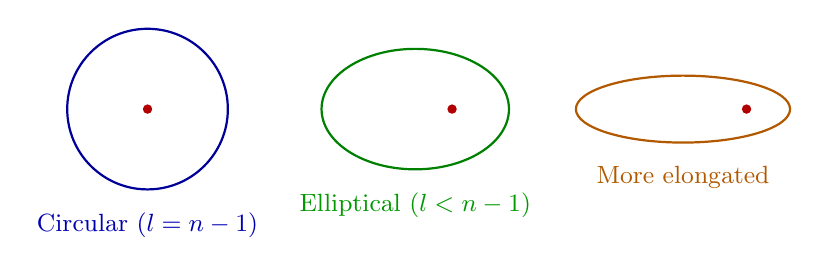
\begin{tikzpicture}[scale=0.85]
    % Circular orbit
    \draw[blue!60!black, thick] (0,0) circle (1.2);
    \fill[red!70!black] (0,0) circle (0.07);
    \node[below, font=\small, blue!70!black] at (0,-1.4)
        {Circular ($l = n-1$)};

    % Elliptical orbit 1
    \draw[green!50!black, thick] (4,0) ellipse (1.4 and 0.9);
    \fill[red!70!black] (4.55,0) circle (0.07);
    \node[below, font=\small, green!60!black] at (4,-1.1)
        {Elliptical ($l < n-1$)};

    % Elliptical orbit 2 (more elongated)
    \draw[orange!70!black, thick] (8,0) ellipse (1.6 and 0.5);
    \fill[red!70!black] (8.95,0) circle (0.07);
    \node[below, font=\small, orange!70!black] at (8,-0.7)
        {More elongated};
\end{tikzpicture}
\end{center}

\medskip
\textbf{Modification 2: Introduction of Azimuthal Quantum
Number $l$}

To describe elliptical orbits, Sommerfeld introduced a second
quantum number called the \textbf{azimuthal (subsidiary)
quantum number} $l$, which defines the \textbf{shape} of the
orbit (ratio of semi-minor to semi-major axis):
\begin{equation*}
    l = 1,\, 2,\, 3,\, \ldots,\, n
\end{equation*}
(in Sommerfeld's original notation; in modern notation
$l = 0, 1, 2, \ldots, n-1$).

For a given principal quantum number $n$, there are $n$
possible values of $l$, corresponding to $n$ possible
orbital shapes. The \textbf{eccentricity} of the ellipse is:
\begin{equation*}
    \frac{b}{a} = \frac{l}{n}
\end{equation*}
where $a$ and $b$ are the semi-major and semi-minor axes.
When $l = n$, the orbit is \textbf{circular}; when $l < n$,
it is \textbf{elliptical}.

\medskip
\textbf{Modification 3: Relativistic Correction}

As electrons move in elongated elliptical orbits, their
velocity \textbf{varies significantly} --- fastest near the
nucleus (perihelion) and slowest far away. Sommerfeld applied
\textbf{Einstein's theory of relativity} to account for the
variation of electron mass with velocity:
\begin{equation*}
    m = \frac{m_0}{\sqrt{1 - v^2/c^2}}
\end{equation*}
This relativistic variation of mass causes the elliptical
orbits to \textbf{precess} (rotate slowly) around the nucleus,
resulting in slightly different energy levels for orbits with
the same $n$ but different $l$.

\medskip
\textbf{Modification 4: Explanation of Fine Structure}

The combination of elliptical orbits and relativistic
correction means that for a given $n$, electrons in orbits
with \textbf{different values of $l$ have slightly different
energies}. Transitions between these sub-levels produce
\textbf{closely spaced spectral lines} --- the fine structure.
For example, for $n = 2$: two possible orbits ($l = 1$
circular, $l = 2$ elliptical) with slightly different
energies, giving rise to two closely spaced lines instead
of one.

\medskip
\textbf{Remaining Limitations of Sommerfeld's Model:}

Despite its improvements, Sommerfeld's model still:
\begin{itemize}[itemsep=2pt]
    \item Failed for \textbf{multi-electron atoms}.
    \item Could not explain the \textbf{Zeeman effect}
    completely.
    \item Did not account for the \textbf{wave nature} of
    the electron.
    \item Could not predict \textbf{relative intensities}
    of spectral lines.
\end{itemize}
These limitations were ultimately resolved only by the
full \textbf{quantum mechanical model} (Schr\"{o}dinger,
1926).

\medskip
\textbf{Summary Table:}
\begin{center}
\begin{tabular}{lll}
\toprule
\textbf{Aspect} & \textbf{Bohr's Model} &
\textbf{Sommerfeld's Model} \\
\midrule
Orbit shape       & Circular only  & Circular and elliptical \\
Quantum numbers   & $n$ only       & $n$ and $l$ \\
Relativistic mass & Not considered & Included \\
Fine structure    & Not explained  & Partially explained \\
Multi-electron    & Fails          & Still fails \\
Wave nature       & Ignored        & Ignored \\
\bottomrule
\end{tabular}
\end{center}

\end{tcolorbox}

\item Deduce de Broglie's equation. Explain with suitable examples the physical significance of the equation. \mk{11}
\yr{CHEM 101 | 2008--09}

\begin{tcolorbox}[enhanced,breakable,ansbox,colback=cA!4,colframe=cA,boxrule=0.8pt,arc=5pt,title={\textbf{Answer}},fonttitle=\bfseries\color{white},colbacktitle=cA]
\textbf{de Broglie's Equation: Deduction and Physical Significance}

\medskip
\textbf{Part 1: Deduction of de Broglie's Equation}

\medskip
\textbf{Step 1: Dual Nature of Light}

It was well established that light exhibits \textbf{dual nature}:
\begin{itemize}[itemsep=2pt]
    \item \textbf{Wave nature:} shown by diffraction and
    interference.
    \item \textbf{Particle nature:} shown by the photoelectric
    effect. Each photon carries energy:
    \begin{equation*}
        E = h\nu \tag{1}
    \end{equation*}
\end{itemize}

\medskip
\textbf{Step 2: Momentum of a Photon}

From Einstein's mass--energy relation:
\begin{equation*}
    E = mc^2 \tag{2}
\end{equation*}

Equating (1) and (2):
\begin{equation*}
    mc^2 = h\nu
    \quad\Rightarrow\quad
    mc = \frac{h\nu}{c} = \frac{h}{\lambda}
    \tag{3}
\end{equation*}

since $\nu/c = 1/\lambda$. Here $mc$ is the
\textbf{momentum $p$} of the photon, so:
\begin{equation*}
    p = \frac{h}{\lambda}
    \quad\Rightarrow\quad
    \lambda = \frac{h}{p} \tag{4}
\end{equation*}

\medskip
\textbf{Step 3: de Broglie's Hypothesis (1924)}

Louis de Broglie argued: if light (a wave) can behave as a
particle, then \textbf{matter (a particle) should also behave
as a wave}. By analogy with equation (4), for a material
particle of mass $m$ moving with velocity $v$, replacing
the photon momentum $mc$ with the particle momentum $mv$:

\begin{equation*}
    \boxed{\lambda = \frac{h}{mv} = \frac{h}{p}}
\end{equation*}

This is the \textbf{de Broglie equation}, where:
\begin{itemize}[itemsep=2pt]
    \item $\lambda$ = de Broglie wavelength of the particle
    \item $h = 6.626 \times 10^{-34}$ J$\cdot$s
    (Planck's constant)
    \item $m$ = mass of the particle (kg)
    \item $v$ = velocity of the particle (m$\cdot$s$^{-1}$)
    \item $p = mv$ = linear momentum (kg$\cdot$m$\cdot$s$^{-1}$)
\end{itemize}

\medskip
\textbf{Step 4: Alternative Forms}

If a particle of charge $q$ is accelerated through a
potential difference $V$:
\begin{equation*}
    \frac{1}{2}mv^2 = qV
    \quad\Rightarrow\quad
    mv = \sqrt{2mqV}
\end{equation*}
\begin{equation*}
    \lambda = \frac{h}{\sqrt{2mqV}}
\end{equation*}

In terms of kinetic energy $E_k = \frac{1}{2}mv^2$:
\begin{equation*}
    \lambda = \frac{h}{\sqrt{2mE_k}}
\end{equation*}

\medskip
\hrule
\medskip

\textbf{Part 2: Physical Significance of de Broglie's Equation}

\medskip
\textbf{1. Wave--Particle Duality of Matter}

The most fundamental significance of de Broglie's equation
is that it establishes \textbf{wave--particle duality} as a
universal property of all matter --- not just light. Every
moving particle, whether an electron, proton, or cricket
ball, has an associated \textbf{matter wave} (de Broglie
wave) whose wavelength is given by $\lambda = h/mv$.

\medskip
\textbf{2. Significance Depends on Mass --- Comparison of
Examples}

\begin{center}
\begin{tabular}{lcccl}
\toprule
\textbf{Object} & \textbf{Mass (kg)} & \textbf{Velocity}
& \textbf{$\lambda$} & \textbf{Observable?} \\
\midrule
Cricket ball  & $0.15$               & $40$ m/s
& $\sim 10^{-34}$ m & No \\
Proton        & $1.67\times10^{-27}$ & $10^5$ m/s
& $\sim 10^{-12}$ m & Barely \\
Electron      & $9.1\times10^{-31}$  & $10^6$ m/s
& $\sim 10^{-9}$ m  & Yes \\
\bottomrule
\end{tabular}
\end{center}

\medskip
\textbf{Example 1: Macroscopic Object (Cricket Ball)}

For a cricket ball of mass $m = 0.15$ kg moving at
$v = 40$ m/s:
\begin{equation*}
    \lambda = \frac{6.626\times10^{-34}}{0.15 \times 40}
    = \frac{6.626\times10^{-34}}{6.0}
    \approx 1.1\times10^{-34}\,\text{m}
\end{equation*}

This is \textbf{far smaller} than any known measurable
length (nuclear diameter $\sim 10^{-15}$ m). Therefore,
the wave nature of macroscopic objects is
\textbf{completely undetectable} --- they behave purely
as classical particles. This is consistent with our
everyday experience.

\medskip
\textbf{Example 2: Electron}

For an electron ($m_e = 9.109\times10^{-31}$ kg)
accelerated through $V = 100$ V:
\begin{equation*}
    \lambda = \frac{h}{\sqrt{2m_e eV}}
    = \frac{6.626\times10^{-34}}
    {\sqrt{2\times9.109\times10^{-31}
    \times1.602\times10^{-19}\times100}}
\end{equation*}
\begin{equation*}
    \lambda = \frac{6.626\times10^{-34}}
    {\sqrt{2.919\times10^{-47}}}
    \approx 1.226\times10^{-10}\,\text{m}
    = 1.226\,\text{\AA}
\end{equation*}

This wavelength is \textbf{comparable to the interatomic
spacing in crystals} ($\sim 1$--$3\,\text{\AA}$). Therefore,
electrons can be \textbf{diffracted by crystals}, exactly
as X-rays are. This was confirmed by:
\begin{itemize}[itemsep=2pt]
    \item \textbf{Davisson--Germer experiment (1927):}
    electrons diffracted by a Ni crystal produced diffraction
    maxima at angles predicted by $\lambda = h/mv$.
    \item \textbf{G.P.\ Thomson's experiment (1927):}
    electrons passed through a gold foil produced concentric
    diffraction rings identical to X-ray patterns.
\end{itemize}

\medskip
\textbf{3. Justification of Bohr's Quantization Condition}

de Broglie's equation provides a \textbf{physical basis} for
Bohr's otherwise arbitrary quantization postulate. For a
stable electron orbit of radius $r$, the electron wave must
form a \textbf{standing wave} --- the circumference must
be an integral multiple of $\lambda$:
\begin{equation*}
    2\pi r = n\lambda = \frac{nh}{mv}
    \quad\Rightarrow\quad
    mvr = \frac{nh}{2\pi}
\end{equation*}
This is exactly \textbf{Bohr's quantization condition},
now derived naturally from wave theory rather than assumed.

\begin{center}
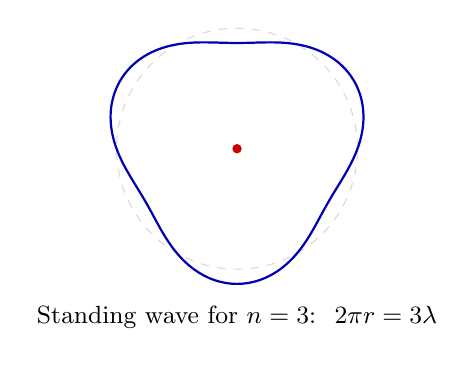
\begin{tikzpicture}[scale=0.85]
    \def\R{1.8}
    \draw[gray!30, dashed] (0,0) circle (\R);
    \draw[blue!70!black, thick, domain=0:360, samples=200]
        plot ({(\R + 0.22*sin(3*\x))*cos(\x)},
             {(\R + 0.22*sin(3*\x))*sin(\x)});
    \fill[red!80!black] (0,0) circle (0.07);
    \node[below, font=\small] at (0,-2.2)
        {Standing wave for $n=3$: $\;2\pi r = 3\lambda$};
\end{tikzpicture}
\end{center}

\medskip
\textbf{4. Foundation of Quantum Mechanics}

de Broglie's equation directly inspired
\textbf{Schr\"{o}dinger} to develop the wave equation for
electrons (1926). The wavefunction $\psi$ in the
Schr\"{o}dinger equation is the mathematical description
of the de Broglie matter wave, and its square $|\psi|^2$
gives the probability density of finding the electron.

\medskip
\textbf{5. Electron Microscopy}

The short de Broglie wavelength of high-energy electrons
is exploited in the \textbf{electron microscope}, which
achieves \textbf{much higher resolution} than optical
microscopes (limited by the longer wavelength of visible
light). This is a direct practical application of de
Broglie's equation.

\medskip
\textbf{Summary of Physical Significance:}
\begin{center}
\begin{tabular}{ll}
\toprule
\textbf{Significance} & \textbf{Implication} \\
\midrule
Wave--particle duality of matter  &
Universal property of all moving objects \\
$\lambda$ negligible for large $m$ &
Classical behaviour of macroscopic objects \\
$\lambda$ significant for electrons &
Electron diffraction observable \\
Justifies Bohr's quantization &
Standing wave condition $\Rightarrow$ $mvr = nh/2\pi$ \\
Foundation of quantum mechanics &
Inspired Schr\"{o}dinger wave equation \\
Electron microscopy &
High-resolution imaging using electron waves \\
\bottomrule
\end{tabular}
\end{center}

\end{tcolorbox}

\item State Heisenberg's Uncertainty principle. Show that the uncertainty principle is applicable only for small particles like the electron. \mk{9}
\yr{CHEM 101 | 2007--08}

\begin{tcolorbox}[enhanced,breakable,ansbox,colback=cA!4,colframe=cA,boxrule=0.8pt,arc=5pt,title={\textbf{Answer}},fonttitle=\bfseries\color{white},colbacktitle=cA]
\textbf{Heisenberg's Uncertainty Principle and Its Applicability
to Small Particles}

\medskip
\textbf{Part 1: Statement of Heisenberg's Uncertainty Principle}

Heisenberg's Uncertainty Principle (1927) states:

\begin{center}
\textit{``It is fundamentally impossible to determine simultaneously
and exactly both the \textbf{position} and the \textbf{momentum}
(or velocity) of a moving particle.''}
\end{center}

Mathematically:
\begin{equation*}
    \boxed{\Delta x \cdot \Delta p \geq \frac{h}{4\pi}}
\end{equation*}

where:
\begin{itemize}[itemsep=2pt]
    \item $\Delta x$ = uncertainty in position
    \item $\Delta p = m\,\Delta v$ = uncertainty in momentum
    \item $h = 6.626\times10^{-34}$ J$\cdot$s = Planck's constant
\end{itemize}

Substituting $\Delta p = m\,\Delta v$:
\begin{equation*}
    \Delta x \cdot m\,\Delta v \geq \frac{h}{4\pi}
    \quad\Rightarrow\quad
    \Delta x \cdot \Delta v \geq \frac{h}{4\pi m}
\end{equation*}

This means: the more precisely the \textbf{position} is known
($\Delta x$ small), the more uncertain the \textbf{momentum}
($\Delta p$ large), and vice versa. This is not a limitation
of instruments --- it is a \textbf{fundamental property of
nature}.

There is also an analogous relation between energy and time:
\begin{equation*}
    \Delta E \cdot \Delta t \geq \frac{h}{4\pi}
\end{equation*}

\medskip
\hrule
\medskip

\textbf{Part 2: Uncertainty Principle Applicable Only to Small
Particles}

\medskip
The uncertainty principle is significant only when the
uncertainties $\Delta x$ and $\Delta v$ are \textbf{comparable
to the actual values} of position and velocity. We show this
with two examples:

\medskip
\textbf{Example 1: Macroscopic Object (Cricket Ball)}

Consider a cricket ball of mass $m = 0.15$ kg. Suppose the
uncertainty in its position is $\Delta x = 10^{-6}$ m
(already far smaller than measurable). Then the minimum
uncertainty in velocity is:
\begin{equation*}
    \Delta v \geq \frac{h}{4\pi m\,\Delta x}
    = \frac{6.626\times10^{-34}}
    {4\pi \times 0.15 \times 10^{-6}}
    \approx 3.5\times10^{-28}\,\text{m/s}
\end{equation*}

This uncertainty is \textbf{negligibly small} compared to
the actual velocity of a cricket ball ($\sim 40$ m/s).
Therefore, the uncertainty principle has
\textbf{no practical significance} for macroscopic objects.

\medskip
\textbf{Example 2: Electron (Small Particle)}

Consider an electron of mass $m_e = 9.109\times10^{-31}$ kg
moving in a hydrogen atom. The diameter of a hydrogen atom
is approximately $10^{-10}$ m, so the maximum uncertainty
in position is $\Delta x \approx 10^{-10}$ m. Then:
\begin{equation*}
    \Delta v \geq \frac{h}{4\pi m_e\,\Delta x}
    = \frac{6.626\times10^{-34}}
    {4\pi \times 9.109\times10^{-31} \times 10^{-10}}
    \approx 5.79\times10^{5}\,\text{m/s}
\end{equation*}

The actual velocity of an electron in the first Bohr orbit
is $v = 2.18\times10^{6}$ m/s. The uncertainty
$\Delta v \approx 5.79\times10^{5}$ m/s is therefore
\textbf{about 27\% of the actual velocity} --- enormously
significant! It is impossible to track the electron's
position and velocity simultaneously with any meaningful
precision.

\medskip
\textbf{Comparison Table:}
\begin{center}
\begin{tabular}{lccl}
\toprule
\textbf{Object} & \textbf{Mass (kg)} & \textbf{$\Delta v$ (m/s)}
& \textbf{Significance} \\
\midrule
Cricket ball & $0.15$              & $3.5\times10^{-28}$
& Negligible --- classically predictable \\
Electron     & $9.1\times10^{-31}$ & $5.8\times10^{5}$
& Enormous --- quantum behaviour \\
\bottomrule
\end{tabular}
\end{center}

\medskip
\textbf{Conclusion:}
The uncertainty principle is \textbf{universally applicable}
to all objects, but its effects are only significant for
\textbf{subatomic particles} like electrons, protons, and
neutrons, where the uncertainties are comparable to the
actual physical quantities. For macroscopic objects, the
product $h/4\pi m$ is so tiny that uncertainties are
completely negligible, and classical mechanics applies
perfectly.

\end{tcolorbox}

\item Discuss the classification of the elements present in the periodic table on the basis of electronic configuration. Mention the characteristics of two important classes of elements. \mk{15}
\yr{CHEM 101 | 2007--08}

\begin{tcolorbox}[enhanced,breakable,ansbox,colback=cA!4,colframe=cA,boxrule=0.8pt,arc=5pt,title={\textbf{Answer}},fonttitle=\bfseries\color{white},colbacktitle=cA]
\textbf{Classification of Elements Based on Electronic
Configuration}

\medskip
\textbf{Introduction}

The modern periodic table classifies all known elements into
\textbf{four blocks} based on which subshell receives the
\textbf{last (differentiating) electron} in their electronic
configuration. These are the \textbf{s, p, d,} and
\textbf{f blocks}.

\medskip
\textbf{1. s-Block Elements}

Elements in which the \textbf{last electron enters the $s$
subshell} of the outermost shell.

General configuration: $ns^{1-2}$

\begin{itemize}[itemsep=2pt]
    \item Includes \textbf{Group 1} (alkali metals: Li, Na,
    K, Rb, Cs, Fr) and \textbf{Group 2} (alkaline earth
    metals: Be, Mg, Ca, Sr, Ba, Ra).
    \item Also includes \textbf{H} and \textbf{He}.
    \item Located on the \textbf{far left} of the periodic
    table (Periods 1--7).
\end{itemize}

\medskip
\textbf{2. p-Block Elements}

Elements in which the \textbf{last electron enters the $p$
subshell} of the outermost shell.

General configuration: $ns^2\,np^{1-6}$

\begin{itemize}[itemsep=2pt]
    \item Includes \textbf{Groups 13--18}.
    \item Contains metals, metalloids, non-metals, and noble
    gases.
    \item Located on the \textbf{right side} of the periodic
    table (Periods 2--7).
\end{itemize}

\medskip
\textbf{3. d-Block Elements (Transition Elements)}

Elements in which the \textbf{last electron enters the $d$
subshell} of the penultimate shell.

General configuration: $(n-1)d^{1-10}\,ns^{1-2}$

\begin{itemize}[itemsep=2pt]
    \item Includes \textbf{Groups 3--12}.
    \item Four series: 3d (Period 4), 4d (Period 5),
    5d (Period 6), 6d (Period 7).
    \item All are \textbf{metals} with variable oxidation
    states, coloured compounds, and catalytic properties.
\end{itemize}

\medskip
\textbf{4. f-Block Elements (Inner Transition Elements)}

Elements in which the \textbf{last electron enters the $f$
subshell} of the anti-penultimate shell.

General configuration: $(n-2)f^{1-14}\,(n-1)d^{0-1}\,ns^2$

\begin{itemize}[itemsep=2pt]
    \item Two series:
    \begin{itemize}
        \item \textbf{Lanthanides} ($4f$ series):
        Ce ($Z=58$) to Lu ($Z=71$), Period 6.
        \item \textbf{Actinides} ($5f$ series):
        Th ($Z=90$) to Lr ($Z=103$), Period 7.
    \end{itemize}
    \item Placed separately at the \textbf{bottom} of the
    periodic table.
    \item All are \textbf{metals}; actinides are mostly
    radioactive.
\end{itemize}

\medskip
\textbf{Summary of Block Classification:}
\begin{center}
\begin{tabular}{cllcc}
\toprule
\textbf{Block} & \textbf{Last electron in}
& \textbf{Groups} & \textbf{Periods}
& \textbf{Max electrons} \\
\midrule
$s$ & $ns^{1-2}$           & 1--2    & 1--7 & 2  \\
$p$ & $ns^2np^{1-6}$       & 13--18  & 2--7 & 6  \\
$d$ & $(n-1)d^{1-10}ns^2$  & 3--12   & 4--7 & 10 \\
$f$ & $(n-2)f^{1-14}$      & (below) & 6--7 & 14 \\
\bottomrule
\end{tabular}
\end{center}

\medskip
\hrule
\medskip

\textbf{Characteristics of Two Important Classes}

\medskip
\textbf{Class 1: s-Block Elements}

\begin{enumerate}[label=(\roman*)]
    \item \textbf{Low ionization energies:} Only 1 or 2
    valence electrons, easily lost to form $M^+$ or $M^{2+}$
    ions. They are the \textbf{most electropositive} elements.

    \item \textbf{Highly reactive metals:} React vigorously
    with water, oxygen, and halogens. Group 1 metals react
    with water to release H$_2$:
    \begin{equation*}
        2\text{Na} + 2\text{H}_2\text{O}
        \to 2\text{NaOH} + \text{H}_2\uparrow
    \end{equation*}

    \item \textbf{Strong reducing agents:} Readily donate
    electrons; reducing power increases down the group.

    \item \textbf{Form ionic compounds:} Compounds are
    predominantly ionic (e.g.\ NaCl, CaCO$_3$), soluble
    in water, and good electrolytes.

    \item \textbf{Flame colours:} Give characteristic
    flame colours (Li: red, Na: yellow, K: violet,
    Ca: brick-red, Sr: crimson, Ba: green).

    \item \textbf{Soft metals with low melting points:}
    Metallic bonding is weak due to only 1--2 valence
    electrons; melting points decrease down the group.
\end{enumerate}

\medskip
\textbf{Class 2: d-Block Elements (Transition Metals)}

\begin{enumerate}[label=(\roman*)]
    \item \textbf{Variable oxidation states:} Both $d$ and
    $s$ electrons participate in bonding, giving multiple
    oxidation states (e.g.\ Mn: $+2$ to $+7$).

    \item \textbf{Coloured compounds:} Partially filled
    $d$ orbitals allow $d$--$d$ electronic transitions
    in the visible region (e.g.\ CuSO$_4$: blue,
    KMnO$_4$: purple).

    \item \textbf{Paramagnetic behaviour:} Unpaired $d$
    electrons give rise to paramagnetism. Magnetic moment:
    \begin{equation*}
        \mu = \sqrt{n(n+2)}\;\text{B.M.}
    \end{equation*}

    \item \textbf{Catalytic properties:} Variable valency
    and surface adsorption make them excellent catalysts
    (Fe in Haber process, V$_2$O$_5$ in Contact process).

    \item \textbf{Complex formation:} Small ionic size,
    high charge, and empty $d$ orbitals allow formation
    of stable complexes with ligands
    (e.g.\ $[\text{Fe(CN)}_6]^{3-}$).

    \item \textbf{High melting and boiling points:} Both
    $s$ and $d$ electrons contribute to strong metallic
    bonding (W has the highest melting point, 3422$^\circ$C).
\end{enumerate}

\end{tcolorbox}


%%══════════════════════════════════════════════════════════════════════
%% S2 — Molecular Geometry
%%══════════════════════════════════════════════════════════════════════
\item What are the postulates of Bohr's atomic model? Based on the postulates, deduce an equation for the calculation of the difference in energies between two levels for an electron in an atom. How far is the Bohr model successful in explaining the spectral properties of an atom? \mk{17}
\yr{CHEM 101 | 2006--07}

\begin{tcolorbox}[enhanced,breakable,ansbox,colback=cA!4,colframe=cA,boxrule=0.8pt,arc=5pt,title={\textbf{Answer}},fonttitle=\bfseries\color{white},colbacktitle=cA]
\textbf{Bohr's Atomic Model: Postulates, Energy Equation and Success}

\medskip
\textbf{Part 1: Postulates of Bohr's Atomic Model (1913)}

\begin{enumerate}[label=(\roman*)]
    \item \textbf{Circular Orbits (Stationary States):}
    Electrons revolve around the nucleus in \textbf{fixed circular
    orbits} called \textbf{stationary states} or \textbf{allowed
    orbits}. While in these orbits, the electron does
    \textbf{not emit or absorb energy}.

    \item \textbf{Quantization of Angular Momentum:}
    An electron can revolve only in those orbits in which its
    \textbf{angular momentum} is an integral multiple of
    $\dfrac{h}{2\pi}$:
    \begin{equation*}
        m_e v r = \frac{nh}{2\pi}
        \qquad (n = 1,\, 2,\, 3,\, \ldots)
    \end{equation*}
    where $n$ is the \textbf{principal quantum number}, $m_e$ is the
    electron mass, $v$ is its velocity, and $r$ is the orbital radius.

    \item \textbf{Energy Emission and Absorption:}
    Energy is emitted or absorbed \textbf{only when an electron
    transitions} from one stationary state to another. When an
    electron jumps from a higher energy level $E_2$ to a lower
    energy level $E_1$, a photon of frequency $\nu$ is emitted:
    \begin{equation*}
        \Delta E = E_2 - E_1 = h\nu
    \end{equation*}

    \item \textbf{Electrostatic Force Provides Centripetal Force:}
    The \textbf{Coulombic attraction} between the nucleus (charge
    $+Ze$) and the electron (charge $-e$) provides the centripetal
    force necessary for circular motion:
    \begin{equation*}
        \frac{m_e v^2}{r} = \frac{Ze^2}{4\pi\varepsilon_0 r^2}
    \end{equation*}
\end{enumerate}

\medskip
\hrule
\medskip

\textbf{Part 2: Derivation of Energy Difference Between Two Levels}

\medskip
\textbf{Step 1: Find the orbital radius $r_n$}

Balancing centripetal and Coulombic forces:
\begin{equation*}
    \frac{m_e v^2}{r} = \frac{Ze^2}{4\pi\varepsilon_0 r^2}
    \quad\Rightarrow\quad
    m_e v^2 r = \frac{Ze^2}{4\pi\varepsilon_0}
    \tag{1}
\end{equation*}

From quantization of angular momentum:
\begin{equation*}
    m_e v r = \frac{nh}{2\pi}
    \quad\Rightarrow\quad
    v = \frac{nh}{2\pi m_e r}
    \tag{2}
\end{equation*}

Substituting (2) into (1):
\begin{equation*}
    m_e \left(\frac{nh}{2\pi m_e r}\right)^2 r
    = \frac{Ze^2}{4\pi\varepsilon_0}
\end{equation*}
\begin{equation*}
    \frac{n^2 h^2}{4\pi^2 m_e r} = \frac{Ze^2}{4\pi\varepsilon_0}
\end{equation*}
\begin{equation*}
    \boxed{r_n = \frac{n^2 h^2 \varepsilon_0}{\pi m_e Z e^2}}
    \tag{3}
\end{equation*}

For hydrogen ($Z = 1$) and $n = 1$:
$r_1 = a_0 = 0.529\,\text{\AA}$ (Bohr radius).

\medskip
\textbf{Step 2: Find the total energy $E_n$}

\textbf{Kinetic energy} of the electron:
\begin{equation*}
    \text{KE} = \frac{1}{2}m_e v^2
    = \frac{Ze^2}{8\pi\varepsilon_0 r}
    \tag{4}
\end{equation*}
(using equation 1: $m_e v^2 = \frac{Ze^2}{4\pi\varepsilon_0 r}$)

\textbf{Potential energy} of the electron:
\begin{equation*}
    \text{PE} = -\frac{Ze^2}{4\pi\varepsilon_0 r}
    \tag{5}
\end{equation*}

\textbf{Total energy:}
\begin{equation*}
    E_n = \text{KE} + \text{PE}
    = \frac{Ze^2}{8\pi\varepsilon_0 r}
    - \frac{Ze^2}{4\pi\varepsilon_0 r}
    = -\frac{Ze^2}{8\pi\varepsilon_0 r}
\end{equation*}

Substituting $r_n$ from equation (3):
\begin{equation*}
    E_n = -\frac{Ze^2}{8\pi\varepsilon_0}
    \cdot \frac{\pi m_e Z e^2}{n^2 h^2 \varepsilon_0}
\end{equation*}

\begin{equation*}
    \boxed{E_n = -\frac{m_e Z^2 e^4}{8\varepsilon_0^2 h^2}
    \cdot \frac{1}{n^2}}
    \tag{6}
\end{equation*}

The negative sign indicates the electron is \textbf{bound} to the
nucleus.

\medskip
\textbf{Step 3: Energy difference between two levels}

When an electron transitions from level $n_2$ (higher) to level
$n_1$ (lower), the energy difference is:
\begin{equation*}
    \Delta E = E_{n_2} - E_{n_1}
    = -\frac{m_e Z^2 e^4}{8\varepsilon_0^2 h^2 n_2^2}
    - \left(-\frac{m_e Z^2 e^4}{8\varepsilon_0^2 h^2 n_1^2}\right)
\end{equation*}

\begin{equation*}
    \boxed{\Delta E = \frac{m_e Z^2 e^4}{8\varepsilon_0^2 h^2}
    \left(\frac{1}{n_1^2} - \frac{1}{n_2^2}\right)}
    \tag{7}
\end{equation*}

Since $\Delta E = h\nu = \dfrac{hc}{\lambda}$, dividing both sides
by $hc$:
\begin{equation*}
    \frac{1}{\lambda} = \frac{m_e Z^2 e^4}{8\varepsilon_0^2 h^3 c}
    \left(\frac{1}{n_1^2} - \frac{1}{n_2^2}\right)
    = R_H Z^2 \left(\frac{1}{n_1^2} - \frac{1}{n_2^2}\right)
\end{equation*}

where $R_H = \dfrac{m_e e^4}{8\varepsilon_0^2 h^3 c}
= 1.097 \times 10^7\,\text{m}^{-1}$ is the \textbf{Rydberg constant}.

\medskip
\hrule
\medskip

\textbf{Part 3: Success of Bohr's Model in Explaining Spectral
Properties}

\begin{enumerate}[label=(\roman*)]
    \item \textbf{Explanation of Hydrogen Spectrum:}
    Bohr's model \textbf{successfully explained} the line spectrum
    of hydrogen. Each spectral line corresponds to a specific
    electron transition $n_2 \to n_1$, giving a photon of definite
    frequency. This perfectly matched the experimentally observed
    spectral lines.

    \item \textbf{Prediction of Spectral Series:}
    The model correctly predicted all known spectral series of
    hydrogen:
    \begin{center}
    \begin{tabular}{llcc}
    \toprule
    \textbf{Series} & \textbf{Region} & $n_1$ & $n_2$ \\
    \midrule
    Lyman    & Ultraviolet  & 1 & 2, 3, 4\ldots \\
    Balmer   & Visible      & 2 & 3, 4, 5\ldots \\
    Paschen  & Infrared     & 3 & 4, 5, 6\ldots \\
    Brackett & Infrared     & 4 & 5, 6, 7\ldots \\
    Pfund    & Far Infrared & 5 & 6, 7, 8\ldots \\
    \bottomrule
    \end{tabular}
    \end{center}

    \item \textbf{Calculation of Rydberg Constant:}
    The model derived the \textbf{Rydberg constant} $R_H$
    theoretically from fundamental constants, and its value
    matched the experimentally determined value perfectly:
    \begin{equation*}
        R_H = 1.097 \times 10^7\,\text{m}^{-1}
    \end{equation*}

    \item \textbf{Hydrogen-like Species:}
    By introducing $Z$ (atomic number) in equation (7), Bohr's
    model successfully explained the spectra of
    \textbf{hydrogen-like ions} such as He$^+$, Li$^{2+}$,
    Be$^{3+}$, etc.

    \item \textbf{Ionization Energy of Hydrogen:}
    Setting $n_1 = 1$ and $n_2 = \infty$ in equation (7):
    \begin{equation*}
        IE = \frac{m_e e^4}{8\varepsilon_0^2 h^2}
        = 13.6\,\text{eV}
    \end{equation*}
    This matches the \textbf{experimentally measured} ionization
    energy of hydrogen (13.6 eV) exactly.

    \item \textbf{Quantization of Energy:}
    The model explained why atoms emit \textbf{discrete line
    spectra} (not continuous spectra) --- because only specific
    energy transitions are allowed between quantized levels.
\end{enumerate}

\medskip
\textbf{Limitations (Brief):}
Despite its successes, Bohr's model fails for multi-electron atoms,
cannot explain the fine structure of spectral lines, violates
Heisenberg's Uncertainty Principle, and does not account for the
wave nature of the electron. These were later resolved by the
\textbf{quantum mechanical model}.

\end{tcolorbox}

\item What is the general electronic configuration of transition elements? Discuss the general properties of transition elements. \mk{10}
\yr{CHEM 101 | 2006--07}

\begin{tcolorbox}[enhanced,breakable,ansbox,colback=cA!4,colframe=cA,boxrule=0.8pt,arc=5pt,title={\textbf{Answer}},fonttitle=\bfseries\color{white},colbacktitle=cA]
\textbf{Electronic Configuration and General Properties of
Transition Elements}

\medskip
\textbf{Part 1: General Electronic Configuration}

Transition elements are those in which the \textbf{$d$ subshell is
partially filled} either in the ground state or in their common
oxidation states. They occupy Groups 3--12 of the periodic table
(3d, 4d, 5d, and 6d series).

The general electronic configuration is:
\begin{equation*}
    (n-1)d^{1-10}\; ns^{1-2}
\end{equation*}

where $n$ is the outermost principal quantum number. The four
transition series are:

\begin{center}
\begin{tabular}{clll}
\toprule
\textbf{Series} & \textbf{Elements} & \textbf{Configuration}
& \textbf{Period} \\
\midrule
1st (3d) & Sc to Zn & $[Ar]\,3d^{1-10}\,4s^{1-2}$ & 4 \\
2nd (4d) & Y to Cd  & $[Kr]\,4d^{1-10}\,5s^{1-2}$ & 5 \\
3rd (5d) & La, Hf to Hg & $[Xe]\,4f^{14}\,5d^{1-10}\,6s^{1-2}$ & 6 \\
4th (6d) & Ac, Rf to Cn & $[Rn]\,5f^{14}\,6d^{1-10}\,7s^{1-2}$ & 7 \\
\bottomrule
\end{tabular}
\end{center}

\textbf{Note:} Some exceptions occur due to extra stability of
half-filled ($d^5$) and completely filled ($d^{10}$) subshells.
For example:
\begin{itemize}[itemsep=2pt]
    \item Cr: $[Ar]\,3d^5\,4s^1$ (not $3d^4\,4s^2$)
    \item Cu: $[Ar]\,3d^{10}\,4s^1$ (not $3d^9\,4s^2$)
\end{itemize}

\medskip
\hrule
\medskip

\textbf{Part 2: General Properties of Transition Elements}

\begin{enumerate}[label=(\roman*)]

    \item \textbf{Metallic Character:}
    All transition elements are \textbf{metals}. They are hard,
    lustrous, malleable, ductile, and good conductors of heat and
    electricity. This is due to the presence of delocalized
    $d$ electrons in addition to $s$ electrons contributing to
    metallic bonding. They generally have \textbf{high melting and
    boiling points} (e.g.\ W has the highest melting point,
    3422$^\circ$C).

    \item \textbf{Variable Oxidation States:}
    Transition metals exhibit \textbf{multiple oxidation states}
    because both $(n-1)d$ and $ns$ electrons can be used in bond
    formation. For example:
    \begin{equation*}
        \text{Mn: } +2,\,+3,\,+4,\,+6,\,+7
        \qquad
        \text{Fe: } +2,\,+3
        \qquad
        \text{Cr: } +2,\,+3,\,+6
    \end{equation*}
    Lower oxidation states are found in covalent compounds while
    higher oxidation states are found with electronegative ligands.

    \item \textbf{Formation of Coloured Compounds:}
    Most transition metal compounds are \textbf{coloured} in the
    solid state or in solution. The colour arises from
    \textbf{$d$--$d$ electronic transitions}: electrons in lower
    $d$ orbitals absorb visible light and are promoted to higher
    $d$ orbitals (crystal field splitting). The complementary
    colour is observed. For example:
    \begin{itemize}[itemsep=2pt]
        \item CuSO$_4$ solution: blue
        \item K$_2$Cr$_2$O$_7$: orange
        \item KMnO$_4$: purple
        \item FeCl$_3$: yellow
    \end{itemize}
    Zn$^{2+}$ ($3d^{10}$) and Sc$^{3+}$ ($3d^0$) are colourless
    because $d$--$d$ transitions are not possible.

    \item \textbf{Formation of Complex Compounds:}
    Transition metals have a strong tendency to form
    \textbf{coordination complexes} with ligands (Lewis bases).
    This is due to:
    \begin{itemize}[itemsep=2pt]
        \item Small ionic size and high charge density.
        \item Availability of empty $d$ orbitals to accept
        lone pairs from ligands.
    \end{itemize}
    Examples: $[\text{Fe(CN)}_6]^{3-}$,
    $[\text{Cu(NH}_3)_4]^{2+}$, $[\text{Co(en)}_3]^{3+}$.

    \item \textbf{Magnetic Properties:}
    Transition metal ions are often \textbf{paramagnetic} due to
    the presence of \textbf{unpaired $d$ electrons}. The magnetic
    moment $\mu$ is given by:
    \begin{equation*}
        \mu = \sqrt{n(n+2)}\;\text{ B.M.}
    \end{equation*}
    where $n$ is the number of unpaired electrons and B.M.\ is
    the Bohr magneton. Compounds with no unpaired electrons are
    \textbf{diamagnetic} (e.g.\ Zn$^{2+}$, $3d^{10}$).

    \item \textbf{Catalytic Properties:}
    Transition metals and their compounds are widely used as
    \textbf{catalysts} due to:
    \begin{itemize}[itemsep=2pt]
        \item Variable oxidation states allowing electron transfer.
        \item Ability to adsorb reactants on their surfaces.
    \end{itemize}
    Examples:
    \begin{itemize}[itemsep=2pt]
        \item Fe in Haber process (N$_2$ + H$_2$ $\to$ NH$_3$)
        \item V$_2$O$_5$ in Contact process (SO$_2$ $\to$ SO$_3$)
        \item Pt/Pd in catalytic converters
        \item Ni in hydrogenation of oils
    \end{itemize}

    \item \textbf{Formation of Alloys:}
    Transition metals readily form \textbf{alloys} with each other
    and with other metals because their atomic radii are similar.
    Alloys are generally harder and more resistant to corrosion
    than pure metals. Examples: steel (Fe + C), brass (Cu + Zn),
    nichrome (Ni + Cr).

    \item \textbf{Atomic and Ionic Radii:}
    Across a transition series, atomic radii \textbf{decrease
    slowly} from left to right (due to increasing nuclear charge)
    but then \textbf{slightly increase} towards the end as
    $d$-$d$ electron repulsion becomes significant. This is in
    contrast to the sharp decrease seen across main group elements.

    \item \textbf{High Ionization Energies:}
    Transition elements have \textbf{higher ionization energies}
    than $s$-block elements but lower than $p$-block non-metals,
    reflecting their intermediate metallic character and the
    effective nuclear charge acting on $d$ electrons.

    \item \textbf{Interstitial Compound Formation:}
    Small atoms such as H, C, N, and B can occupy
    \textbf{interstitial voids} in the transition metal crystal
    lattice, forming \textbf{interstitial compounds}
    (e.g.\ TiC, Fe$_3$C, TiN). These compounds are harder and
    have higher melting points than the pure metals.

\end{enumerate}

\medskip
\textbf{Summary Table:}
\begin{center}
\begin{tabular}{ll}
\toprule
\textbf{Property} & \textbf{Reason} \\
\midrule
Variable oxidation states  & Participation of $d$ and $s$ electrons \\
Coloured compounds         & $d$--$d$ transitions in visible range \\
Complex formation          & Empty $d$ orbitals, high charge density \\
Paramagnetism              & Unpaired $d$ electrons \\
Catalytic activity         & Variable valency, surface adsorption \\
High melting points        & Strong metallic bonding with $d$ electrons \\
\bottomrule
\end{tabular}
\end{center}

\end{tcolorbox}

\item Deduce de Broglie's equation. With a suitable example, discuss the applicability of the equation in the case of electron-like particles. \mk{9}
\yr{CHEM 101 | 2006--07}

\begin{tcolorbox}[enhanced,breakable,ansbox,colback=cA!4,colframe=cA,boxrule=0.8pt,arc=5pt,title={\textbf{Answer}},fonttitle=\bfseries\color{white},colbacktitle=cA]
\textbf{de Broglie's Equation: Deduction and Applicability}

\medskip
\textbf{Part 1: Deduction of de Broglie's Equation}

\medskip
\textbf{Step 1: Energy of a Photon (Particle Nature of Light)}

From Planck's quantum theory, the energy of a photon of frequency
$\nu$ is:
\begin{equation*}
    E = h\nu \tag{1}
\end{equation*}

From Einstein's mass--energy relation:
\begin{equation*}
    E = mc^2 \tag{2}
\end{equation*}

Equating (1) and (2):
\begin{equation*}
    mc^2 = h\nu \tag{3}
\end{equation*}

\medskip
\textbf{Step 2: Introduce Wavelength}

Since $\nu = \dfrac{c}{\lambda}$, substituting into (3):
\begin{equation*}
    mc^2 = h \cdot \frac{c}{\lambda}
    \quad\Rightarrow\quad
    mc = \frac{h}{\lambda}
    \quad\Rightarrow\quad
    \lambda = \frac{h}{mc} \tag{4}
\end{equation*}

Here $mc$ is the \textbf{momentum} $p$ of the photon.

\medskip
\textbf{Step 3: Extend to Material Particles (de Broglie, 1924)}

de Broglie proposed that \textbf{every moving material particle},
like a photon, also has an associated wave. By analogy with
equation (4), for a particle of mass $m$ moving with velocity $v$,
the photon momentum $mc$ is replaced by the particle momentum
$mv$:

\begin{equation*}
    \boxed{\lambda = \frac{h}{mv} = \frac{h}{p}}
\end{equation*}

This is \textbf{de Broglie's equation}, where:
\begin{itemize}[itemsep=2pt]
    \item $\lambda$ = de Broglie wavelength of the particle
    \item $h$ = Planck's constant ($6.626 \times 10^{-34}$ J$\cdot$s)
    \item $m$ = mass of the particle
    \item $v$ = velocity of the particle
    \item $p = mv$ = linear momentum of the particle
\end{itemize}

The equation beautifully connects the \textbf{wave property}
($\lambda$) with the \textbf{particle property} ($p$), establishing
the dual nature of matter.

\medskip
\textbf{Step 4: Relation to Kinetic Energy}

If a particle is accelerated through a potential difference $V$
(in volts), its kinetic energy is:
\begin{equation*}
    \frac{1}{2}mv^2 = eV
    \quad\Rightarrow\quad
    mv = \sqrt{2meV}
\end{equation*}

Substituting into de Broglie's equation:
\begin{equation*}
    \lambda = \frac{h}{\sqrt{2meV}}
\end{equation*}

\medskip
\hrule
\medskip

\textbf{Part 2: Applicability to Electron-like Particles}

\medskip
\textbf{Example: de Broglie Wavelength of an Electron}

Consider an electron (mass $m_e = 9.109 \times 10^{-31}$ kg)
accelerated through a potential difference of $V = 100$ V.

\textbf{Calculating the wavelength:}
\begin{equation*}
    \lambda = \frac{h}{\sqrt{2m_e eV}}
\end{equation*}
\begin{equation*}
    \lambda = \frac{6.626 \times 10^{-34}}
    {\sqrt{2 \times 9.109 \times 10^{-31}
    \times 1.602 \times 10^{-19} \times 100}}
\end{equation*}
\begin{equation*}
    \lambda = \frac{6.626 \times 10^{-34}}
    {\sqrt{2.919 \times 10^{-47}}}
    = \frac{6.626 \times 10^{-34}}{1.708 \times 10^{-23.5}}
\end{equation*}
\begin{equation*}
    \lambda \approx 1.226 \times 10^{-10}\,\text{m}
    = 1.226\,\text{\AA}
\end{equation*}

This wavelength is \textbf{comparable to the spacing between atoms
in a crystal} ($\sim 1$--$3\,\text{\AA}$), which is why electrons
can be \textbf{diffracted by crystals} --- directly proving their
wave nature.

\medskip
\textbf{Comparison with Macroscopic Objects:}

\begin{center}
\begin{tabular}{lccl}
\toprule
\textbf{Object} & \textbf{Mass (kg)} & \textbf{Velocity (m/s)}
& \textbf{$\lambda$} \\
\midrule
Cricket ball  & $0.15$               & $40$   &
$\sim 10^{-34}$ m (undetectable) \\
Proton        & $1.67\times10^{-27}$ & $10^5$ &
$\sim 10^{-12}$ m \\
Electron      & $9.1\times10^{-31}$  & $10^6$ &
$\sim 10^{-9}$ m (observable) \\
\bottomrule
\end{tabular}
\end{center}

For \textbf{macroscopic objects} (cricket ball, car, etc.), the
de Broglie wavelength is \textbf{negligibly small}
($\sim 10^{-34}$ m), far below any measurable scale. Hence their
wave nature is \textbf{undetectable} in practice.

For \textbf{subatomic particles} like electrons, the wavelength
is \textbf{comparable to atomic dimensions}, making wave behaviour
\textbf{physically significant and observable}.

\medskip
\textbf{Experimental Verification:}

\begin{enumerate}[label=(\roman*)]
    \item \textbf{Davisson--Germer Experiment (1927):}
    Electrons were diffracted by a nickel crystal, producing
    diffraction maxima at angles predicted exactly by de Broglie's
    equation. The measured $\lambda$ matched $h/mv$ perfectly.

    \item \textbf{G.P.\ Thomson's Experiment (1927):}
    Electrons passed through a thin gold foil produced concentric
    diffraction rings, identical to X-ray diffraction patterns,
    confirming the wave nature of electrons.
\end{enumerate}

\medskip
\textbf{Application in Bohr's Model:}

de Broglie's equation provides a \textbf{physical justification}
for Bohr's quantization condition. For a stable circular orbit of
radius $r$, the electron wave must form a \textbf{standing wave}:
\begin{equation*}
    2\pi r = n\lambda = \frac{nh}{mv}
    \quad\Rightarrow\quad
    mvr = \frac{nh}{2\pi}
\end{equation*}
This is exactly \textbf{Bohr's quantization postulate}, now derived
naturally from wave theory.

\medskip
\textbf{Conclusion:}
de Broglie's equation $\lambda = h/mv$ is highly applicable to
electron-like particles because their small mass gives a wavelength
large enough to be experimentally observed and utilized in electron
microscopy, electron diffraction, and quantum mechanical modelling
of atomic structure.

\end{tcolorbox}

\item How would you conceive the idea of having an electron cloud around the nucleus of an atom? \mk{6}
\yr{CHEM 101 | 2006--07}

\begin{tcolorbox}[enhanced,breakable,ansbox,colback=cA!4,colframe=cA,boxrule=0.8pt,arc=5pt,title={\textbf{Answer}},fonttitle=\bfseries\color{white},colbacktitle=cA]
\textbf{The Concept of Electron Cloud Around the Nucleus}

\medskip
\textbf{1. Failure of Bohr's Fixed Orbit Model}

Bohr's model assumed that electrons move in \textbf{fixed circular
orbits} with a precisely defined position and velocity at every
instant. However, \textbf{Heisenberg's Uncertainty Principle}
(1927) showed that it is \textbf{fundamentally impossible} to
determine the exact position and momentum of an electron
simultaneously:
\begin{equation*}
    \Delta x \cdot \Delta p \geq \frac{h}{4\pi}
\end{equation*}
Since position and momentum cannot both be known precisely, the
concept of a fixed orbit is \textbf{physically meaningless} for
an electron. This necessitated a new model.

\medskip
\textbf{2. The Quantum Mechanical Description}

In the quantum mechanical model, the behaviour of an electron is
described by the \textbf{wavefunction} $\psi$, obtained by solving
the Schr\"{o}dinger wave equation:
\begin{equation*}
    \nabla^2\psi + \frac{8\pi^2 m}{h^2}(E - V)\psi = 0
\end{equation*}

According to \textbf{Born's interpretation}, the wavefunction
itself has no direct physical meaning, but its square $|\psi|^2$
gives the \textbf{probability density} of finding the electron
at a given point in space:
\begin{equation*}
    \text{Probability} \propto |\psi|^2 \cdot dV
\end{equation*}
where $dV$ is a small volume element around the point.

\medskip
\textbf{3. Conception of the Electron Cloud}

Since the electron does not follow a fixed path, its position at
any instant is \textbf{uncertain}. Over time, the electron can
be found at various locations around the nucleus with different
probabilities. This gives rise to the idea of an
\textbf{electron cloud}:

\begin{itemize}[itemsep=3pt]
    \item The electron cloud is a \textbf{three-dimensional
    probability map} around the nucleus, representing all the
    possible locations of the electron.

    \item Regions where $|\psi|^2$ is \textbf{large} appear as
    \textbf{dense} parts of the cloud --- the electron is most
    likely to be found here.

    \item Regions where $|\psi|^2$ is \textbf{small} appear as
    \textbf{diffuse} parts of the cloud --- the electron is
    unlikely to be found here.

    \item The cloud has \textbf{no sharp boundary} --- there is
    always a small but non-zero probability of finding the
    electron far from the nucleus.
\end{itemize}

\begin{center}
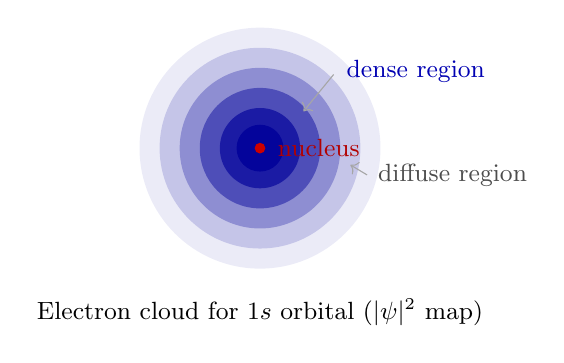
\begin{tikzpicture}[scale=0.85]
    % Electron cloud: concentric shaded circles
    \foreach \r/\op in {1.8/8, 1.5/16, 1.2/28, 0.9/45, 0.6/65, 0.35/85}{
        \fill[blue!60!black, opacity=\op/100] (0,0) circle (\r);
    }
    % Nucleus
    \fill[red!80!black] (0,0) circle (0.08);
    \node[right, font=\small, red!70!black] at (0.12, 0)
        {nucleus};
    % Annotation
    \draw[->, gray!70] (1.1, 1.1) -- (0.65, 0.55);
    \node[right, font=\small, blue!70!black] at (1.15, 1.15)
        {dense region};
    \draw[->, gray!70] (1.6, -0.4) -- (1.35, -0.25);
    \node[right, font=\small, gray!60!black] at (1.62,-0.4)
        {diffuse region};
    \node[below, font=\small] at (0,-2.1)
        {Electron cloud for $1s$ orbital ($|\psi|^2$ map)};
\end{tikzpicture}
\end{center}

\medskip
\textbf{4. Orbital vs.\ Cloud}

The electron cloud defines the \textbf{atomic orbital} ---
the region of space where the probability of finding the electron
is \textbf{95\%} or more. It replaces Bohr's sharp circular orbit
with a \textbf{fuzzy, probabilistic region} that correctly
reflects the quantum mechanical nature of the electron.

\medskip
\textbf{Conclusion:}
The electron cloud arises naturally from the inability to assign
a fixed path to the electron (Heisenberg's principle) and from
the probabilistic interpretation of the wavefunction ($|\psi|^2$).
It represents the \textbf{spatial distribution of the probability}
of finding the electron, giving the atom its characteristic
``cloud-like'' electron density around the nucleus.

\end{tcolorbox}
\end{enumerate}
\newpage

\secdivider{Section S2}{Molecular Geometry}{cB}{cB}
\markboth{S2 --- Molecular Geometry}{}
  \label{sec:S2}
\section{S2 --- Molecular Geometry}

\begin{enumerate}
\item Predict the shapes of (i) SO$_3^{2-}$ and (ii) PCl$_4^+$ ions showing all the necessary steps. \mk{10}
\yr{CHEM 113 | 2020--21}
\begin{tcolorbox}[enhanced,breakable,ansbox,colback=cB!4,colframe=cB,boxrule=0.8pt,arc=5pt,title={\textbf{Answer}},fonttitle=\bfseries\color{white},colbacktitle=cB]
\textbf{Using VSEPR Theory:} The shape is determined by the number of bond pairs (BP) and lone pairs (LP) around the central atom.

\medskip
\textbf{(i) SO$_3^{2-}$ (Sulphite ion)}

\begin{enumerate}[label=\textbf{Step \arabic*.}, leftmargin=*, itemsep=4pt]
  \item \textbf{Valence electrons:}\\
        S $= 6$, O $= 6\times3 = 18$, charge $= +2$\\
        Total $= 6 + 18 + 2 = 26$ electrons

  \item \textbf{Lewis structure:}
        S is the central atom, bonded to 3 oxygen atoms.\\
        After forming 3 S--O bonds (6 electrons used) and completing octets on O atoms (18 electrons), remaining $= 26 - 6 - 18 = 2$ electrons $\rightarrow$ 1 lone pair on S.

  \item \textbf{Electron geometry count:}\\
        BP $= 3$, LP $= 1$ $\Rightarrow$ Total electron pairs $= 4$\\
        $\Rightarrow$ Electron geometry: \textbf{Tetrahedral}

  \item \textbf{Molecular shape:}\\
        With 3 BP and 1 LP $\Rightarrow$ \textbf{Trigonal Pyramidal}\\
        Bond angle $< 109.5^\circ$ (due to LP--BP repulsion) $\approx 106^\circ$
\end{enumerate}

\[
\chemleft[
  \chemfig{
    \charge{90=\:}{S} % লোন পেয়ার উপরে
    (=[:270]O)        % নিচে ডাবল বন্ড
    (<[:210]O)        % সামনে/বামে ওয়েজ বন্ড
    (<:[:330]O)       % পেছনে/ডানে ড্যাশ বন্ড
  }
\chemright]^{2-}
\]


\medskip
\textbf{(ii) PCl$_4^+$ (Tetrachlorophosphorus cation)}

\begin{enumerate}[label=\textbf{Step \arabic*.}, leftmargin=*, itemsep=4pt]
  \item \textbf{Valence electrons:}\\
        P $= 5$, Cl $= 7\times4 = 28$, charge $= -1$\\
        Total $= 5 + 28 - 1 = 32$ electrons

  \item \textbf{Lewis structure:}
        P is the central atom, bonded to 4 Cl atoms.\\
        4 P--Cl bonds use $8$ electrons; remaining $24$ electrons fill lone pairs on Cl atoms (6 each). No lone pair remains on P.

  \item \textbf{Electron geometry count:}\\
        BP $= 4$, LP $= 0$ $\Rightarrow$ Total electron pairs $= 4$\\
        $\Rightarrow$ Electron geometry: \textbf{Tetrahedral}

  \item \textbf{Molecular shape:}\\
        With 4 BP and 0 LP $\Rightarrow$ \textbf{Tetrahedral}\\
        Bond angle $= 109.5^\circ$
\end{enumerate}

\[
\chemleft[
  \chemfig{
    P
    (-[:90]Cl)   % সোজা উপরে
    (-[:210]Cl)  % বামে নিচে
    (<[:330]Cl)  % সামনে/ডানে ওয়েজ বন্ড
    (<:[:270]Cl) % পেছনে/নিচে ড্যাশ বন্ড
  }
\chemright]^{+}
\]

\end{tcolorbox}

\item Sketch the shape or three-dimensional structure of each of the following: BrO$_3^-$ and AsF$_4^-$. Name the shapes and state the status of hybridization in the central atoms. \mk{6}
\yr{CHEM 113 | 2017--18}

\begin{tcolorbox}[enhanced,breakable,ansbox,colback=cB!4,colframe=cB,boxrule=0.8pt,arc=5pt,title={\textbf{Answer}},fonttitle=\bfseries\color{white},colbacktitle=cB]

%---------------------------------------------------------
\textbf{(i) BrO$_3^-$ (Bromate ion)}
%---------------------------------------------------------

\begin{itemize}[itemsep=2pt]
  \item \textbf{Valence electrons:} $7 + 3\times6 + 1 = 26$ electrons
  \item Br is the central atom bonded to 3 O atoms; 1 LP on Br
  \item BP $= 3$, LP $= 1$ $\Rightarrow$ Total electron pairs $= 4$
  \item \textbf{Hybridization of Br:} $sp^3$
  \item Electron geometry: Tetrahedral
  \item \textbf{Molecular Shape: Trigonal Pyramidal}, bond angle $< 109.5^\circ \approx 106^\circ$
\end{itemize}

\[
\chemleft[
  \chemfig{
    \charge{90=\:}{Br} % ব্রোমিনের উপর লোন পেয়ার
    (=[:270]O)         % নিচে ডাবল বন্ড
    (=[:210]O)         % সামনে/বামে ডাবল বন্ড
    (<:[:330]O)        % পেছনে/ডানে ড্যাশ সিঙ্গেল বন্ড
  }
\chemright]^{-}
\]

\medskip 
%---------------------------------------------------------
\textbf{(ii) AsF$_4^-$ (Tetrafluoroarsenate ion)}
%---------------------------------------------------------

\begin{itemize}[itemsep=2pt]
  \item \textbf{Valence electrons:} $5 + 4\times7 + 1 = 34$ electrons
  \item As is the central atom bonded to 4 F atoms; 1 LP on As
  \item BP $= 4$, LP $= 1$ $\Rightarrow$ Total electron pairs $= 5$
  \item \textbf{Hybridization of As:} $sp^3d$
  \item Electron geometry: Trigonal Bipyramidal
  \item LP occupies equatorial position (less repulsion)
  \item \textbf{Molecular Shape: See-Saw (Sawhorse)}, \\
        axial bond angle $\approx 180^\circ$, equatorial bond angle $\approx 120^\circ$,\\
        axial--equatorial angle $< 90^\circ$
\end{itemize}

\[
\chemleft[
  \chemfig{
    \charge{180=\:}{As} % লোন পেয়ার (Equatorial, বামে)
    (-[:90]F)           % Axial top
    (-[:270]F)          % Axial bottom
    (<[:330]F)          % Equatorial front/right (wedge)
    (<:[:30]F)          % Equatorial back/right (dash)
  }
\chemright]^{-}
\]
\begin{center}
  \small \textit{See-Saw Shape} \quad ($sp^3d$)
\end{center}

\end{tcolorbox}

\item Draw the trigonal bipyramidal geometry and mark the axial and equatorial positions. Which position is suitable for the accommodation of a lone pair in the system? Why? \mk{6}
\yr{CHEM 113 | 2016--17}

\begin{tcolorbox}[enhanced,breakable,ansbox,colback=cB!4,colframe=cB,boxrule=0.8pt,arc=5pt,title={\textbf{Answer}},fonttitle=\bfseries\color{white},colbacktitle=cB]

%---------------------------------------------------------
\textbf{Trigonal Bipyramidal Geometry}
%---------------------------------------------------------

In trigonal bipyramidal geometry, the central atom has \textbf{5 electron pairs} arranged via $sp^3d$ hybridization. There are two distinct positions:

\begin{itemize}[itemsep=2pt, label=\textcolor{cB}{$\bullet$}]
  \item \textbf{Axial positions (2):} Above and below the equatorial plane, bond angle $= 180^\circ$ with each other, $90^\circ$ with equatorial bonds.
  \item \textbf{Equatorial positions (3):} In the trigonal plane, bond angle $= 120^\circ$ with each other, $90^\circ$ with axial bonds.
\end{itemize}

\begin{center}
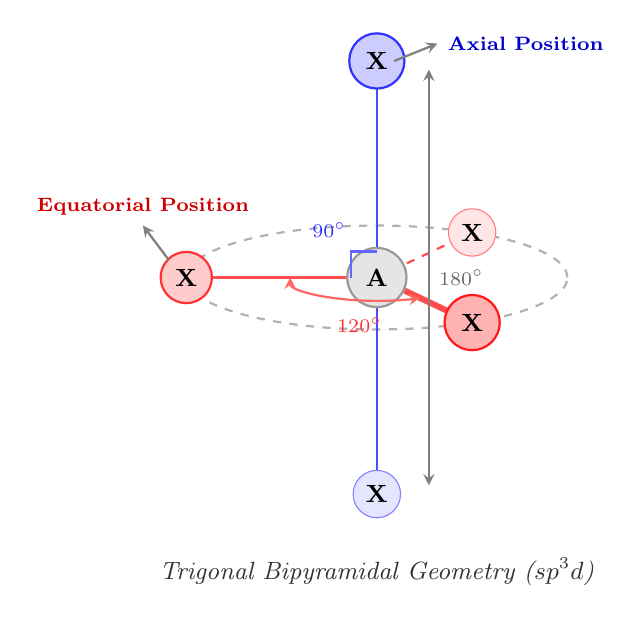
\begin{tikzpicture}[>=stealth, font=\small, scale=1.1]

  % Define exact 3D projection coordinates
  \coordinate (C)     at (0,0);
  \coordinate (AxTop) at (0, 2.5);
  \coordinate (AxBot) at (0,-2.5);
  
  % Equatorial plane coordinates (Ellipse: x-rad=2.2, y-rad=0.6)
  \coordinate (EqL)   at (-2.2, 0);       % 180 degrees (Left)
  \coordinate (EqBR)  at (1.1, 0.52);     % 60 degrees (Back Right)
  \coordinate (EqFR)  at (1.1, -0.52);    % 300 degrees (Front Right)

  % Draw dashed equatorial plane ellipse for 3D visual guide
  \draw[dashed, gray!60, thick] (0,0) ellipse (2.2cm and 0.6cm);

  % 1. BACK EQUATORIAL (Bond & Atom) - Drawn first to stay behind
  \draw[thick, dashed, red!70] (C) -- (EqBR);
  \node[circle, fill=red!10, draw=red!50, inner sep=2.5pt] at (EqBR) {\textbf{X}};

  % 2. BOTTOM AXIAL (Bond & Atom)
  \draw[thick, blue!70] (C) -- (AxBot);
  \node[circle, fill=blue!10, draw=blue!50, inner sep=2.5pt] at (AxBot) {\textbf{X}};

  % 3. CENTRAL ATOM
  \node[circle, fill=gray!20, draw=gray!80, thick, inner sep=4pt] (Center) at (C) {\textbf{A}};

  % 4. LEFT EQUATORIAL (Bond & Atom)
  \draw[thick, red!70] (Center) -- (EqL);
  \node[circle, fill=red!20, draw=red!80, thick, inner sep=3pt] at (EqL) {\textbf{X}};

  % 5. FRONT RIGHT EQUATORIAL (Thick Wedge Bond & Atom)
  \draw[line width=2.2pt, red!70] (Center) -- (EqFR); 
  \node[circle, fill=red!30, draw=red!90, thick, inner sep=3.5pt] at (EqFR) {\textbf{X}};

  % 6. TOP AXIAL (Bond & Atom)
  \draw[thick, blue!70] (Center) -- (AxTop);
  \node[circle, fill=blue!20, draw=blue!80, thick, inner sep=3.5pt] at (AxTop) {\textbf{X}};

  % --- ANGLE LABELS ---
  % 90 Degree Angle Marker (Top to Left)
  \draw[thick, blue!60] (-0.3, 0) -- (-0.3, 0.3) -- (0, 0.3);
  \node[font=\scriptsize\bfseries, blue!80] at (-0.55, 0.55) {$90^\circ$};

  % 120 Degree Angle Arc (Left to Front Right on the 3D plane)
  \draw[thick, red!60, <->] (-1.0, 0) arc (180:300:1.0cm and 0.27cm);
  \node[font=\scriptsize\bfseries, red!80] at (-0.2, -0.55) {$120^\circ$};

  % --- TEXT LABELS ---
  \draw[->, gray, thick] (AxTop) ++(0.2, 0) -- ++(0.5, 0.2) 
        node[right, font=\scriptsize\bfseries, text=blue!80!black] {Axial Position};
  \draw[->, gray, thick] (EqL) ++(-0.2, 0.2) -- ++(-0.3, 0.4) 
        node[above, font=\scriptsize\bfseries, text=red!80!black] {Equatorial Position};

  % 180 Degree Brace
  \draw[<->, gray, thick] (0.6, 2.4) -- (0.6, -2.4) 
        node[midway, right, font=\scriptsize\bfseries, text=gray!80!black] {$180^\circ$};

  \node[font=\small\itshape, text=black!80] at (0,-3.4) {Trigonal Bipyramidal Geometry ($sp^3d$)};

\end{tikzpicture}
\end{center}

\medskip
%---------------------------------------------------------
\textbf{Suitable Position for Lone Pair: Equatorial}
%---------------------------------------------------------

The \textbf{equatorial position} is preferred for lone pair accommodation. The reasons are:

\begin{itemize}[itemsep=4pt, label=\textcolor{cB}{$\bullet$}]

  \item \textbf{Fewer repulsions:} A lone pair in the \textit{equatorial} position experiences only \textbf{2 repulsions at $90^\circ$} (with 2 axial bond pairs). \\
        A lone pair in the \textit{axial} position would experience \textbf{3 repulsions at $90^\circ$} (with 3 equatorial bond pairs).

  \item \textbf{LP--BP repulsion is stronger} than BP--BP repulsion, so minimizing the number of $90^\circ$ LP--BP interactions lowers the overall energy of the molecule.

  \item \textbf{More space:} Equatorial positions have $120^\circ$ angles between them, providing more room for the spatially diffuse lone pair cloud.

\end{itemize}

\begin{center}
\renewcommand{\arraystretch}{1.4}
\begin{tabular}{lcc}
\toprule
\textbf{LP Position} & \textbf{No.\ of $90^\circ$ LP--BP interactions} & \textbf{Stability} \\
\midrule
Axial       & 3 & Less stable \\
Equatorial  & 2 & \textbf{More stable} $\checkmark$ \\
\bottomrule
\end{tabular}
\end{center}

\medskip
\textbf{Conclusion:} Lone pairs always occupy \textbf{equatorial positions} in trigonal bipyramidal systems to minimize repulsion and maximize stability. This is why molecules like SF$_4$ adopt a \textit{see-saw} shape and ClF$_3$ adopts a \textit{T-shape}.

\end{tcolorbox}

\item Draw the geometry of the following and predict the angles: (i) PO$_4^{3-}$ (ii) I$_3^-$. \mk{6}
\yr{CHEM 113 | 2016--17}

\begin{tcolorbox}[enhanced,breakable,ansbox,colback=cB!4,colframe=cB,boxrule=0.8pt,arc=5pt,title={\textbf{Answer}},fonttitle=\bfseries\color{white},colbacktitle=cB]

%---------------------------------------------------------
\textbf{(i) PO$_4^{3-}$ (Phosphate ion)}
%---------------------------------------------------------

\begin{itemize}[itemsep=2pt]
  \item \textbf{Valence electrons:} $5 + 4\times6 + 3 = 32$ electrons
  \item P is the central atom bonded to 4 O atoms
  \item BP $= 4$, LP $= 0$ $\Rightarrow$ Total electron pairs $= 4$
  \item \textbf{Hybridization:} $sp^3$
  \item Electron geometry $=$ Molecular geometry
  \item \textbf{Shape: Tetrahedral}, bond angle $= 109.5^\circ$
\end{itemize}

\[ 
\left[ \chemfig{P(-[:210]O)(<:[:330]O)(<[:300]O)(-[:90]O)} \right]^{3-}
\]

\medskip
%---------------------------------------------------------
\textbf{(ii) I$_3^-$ (Triiodide ion)}
%---------------------------------------------------------

\begin{itemize}[itemsep=2pt]
  \item \textbf{Valence electrons:} $3\times7 + 1 = 22$ electrons
  \item Central I is bonded to 2 terminal I atoms; \textbf{3 LP} on central I
  \item BP $= 2$, LP $= 3$ $\Rightarrow$ Total electron pairs $= 5$
  \item \textbf{Hybridization:} $sp^3d$
  \item Electron geometry: Trigonal Bipyramidal
  \item LP occupy all 3 equatorial positions (minimize repulsion)
  \item \textbf{Shape: Linear}, bond angle $= 180^\circ$
\end{itemize}

\[
\left[
  \chemfig{\charge{90=\:,210=\:,330=\:}{I}(-[:0]I)(-[:180]I)}
  \right]^-
\]

\begin{center}
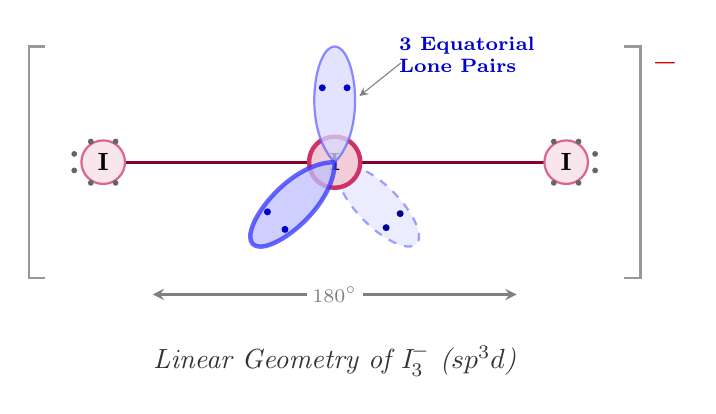
\begin{tikzpicture}[>=stealth, font=\small, scale=1.05]

  % Define a macro for 3D lone pair lobes: \lobe{angle}{fill}{draw}{line style}
  \def\lobe#1#2#3#4{
    \filldraw[rotate=#1, fill=#2, draw=#3, #4, opacity=0.75]
      (0,0) .. controls (0.4, 0.4) and (1.4, 0.25) .. (1.4, 0)
            .. controls (1.4,-0.25) and (0.4,-0.4) .. (0,0);
  }

  % 1. BACK EQUATORIAL LOBE (Drawn first so it stays behind the bonds)
  \lobe{315}{blue!10}{blue!50}{dashed, thick}
  \fill[rotate=315, blue!60!black] (1.0, 0.12) circle (1.2pt);
  \fill[rotate=315, blue!60!black] (1.0,-0.12) circle (1.2pt);

  % 2. AXIAL BONDS
  \draw[line width=1.2pt, purple!70!black] (-2.8, 0) -- (2.8, 0);

  % 3. CENTRAL IODINE ATOM
  \node[circle, fill=purple!20, draw=purple!80, ultra thick, inner sep=4pt] (Ic) at (0,0) {\textbf{I}};

  % 4. TOP EQUATORIAL LOBE
  \lobe{90}{blue!15}{blue!60}{thick}
  \fill[rotate=90, blue!80!black] (0.9, 0.15) circle (1.2pt);
  \fill[rotate=90, blue!80!black] (0.9,-0.15) circle (1.2pt);

  % 5. FRONT EQUATORIAL LOBE (Wedge style for 3D pop-out effect)
  \lobe{225}{blue!25}{blue!80}{ultra thick}
  \fill[rotate=225, blue!80!black] (1.0, 0.15) circle (1.2pt);
  \fill[rotate=225, blue!80!black] (1.0,-0.15) circle (1.2pt);

  % 6. TERMINAL IODINE ATOMS
  \node[circle, fill=purple!10, draw=purple!60, thick, inner sep=3pt] (I1) at (-2.8, 0) {\textbf{I}};
  \node[circle, fill=purple!10, draw=purple!60, thick, inner sep=3pt] (I2) at ( 2.8, 0) {\textbf{I}};

  % 7. TERMINAL ATOM LONE PAIRS (Properly arranged dots)
  % Left I lone pairs
  \fill[gray!80!black] (-2.95,  0.25) circle (1pt); \fill[gray!80!black] (-2.65,  0.25) circle (1pt);
  \fill[gray!80!black] (-2.95, -0.25) circle (1pt); \fill[gray!80!black] (-2.65, -0.25) circle (1pt);
  \fill[gray!80!black] (-3.15,  0.10) circle (1pt); \fill[gray!80!black] (-3.15, -0.10) circle (1pt);
  % Right I lone pairs
  \fill[gray!80!black] (2.95,  0.25) circle (1pt); \fill[gray!80!black] (2.65,  0.25) circle (1pt);
  \fill[gray!80!black] (2.95, -0.25) circle (1pt); \fill[gray!80!black] (2.65, -0.25) circle (1pt);
  \fill[gray!80!black] (3.15,  0.10) circle (1pt); \fill[gray!80!black] (3.15, -0.10) circle (1pt);

  % 8. BRACKETS AND CHARGE (For the overall ion)
  \draw[thick, gray!80] (-3.5, 1.4) -- (-3.7, 1.4) -- (-3.7, -1.4) -- (-3.5, -1.4);
  \draw[thick, gray!80] ( 3.5, 1.4) -- ( 3.7, 1.4) -- ( 3.7, -1.4) -- ( 3.5, -1.4);
  \node[font=\large\bfseries, text=red!80!black] at (4.0, 1.2) {$-$};

  % 9. LABELS & ARROWS
  \draw[<->, gray, thick] (-2.2, -1.6) -- (2.2, -1.6) 
        node[midway, fill=white, inner sep=2pt, font=\scriptsize\bfseries] {$180^\circ$};
        
  \draw[->, gray, thin] (0.8, 1.2) -- (0.3, 0.8);
  \node[font=\scriptsize\bfseries, text=blue!80!black, align=left] at (1.6, 1.3) {3 Equatorial\\Lone Pairs};

  % 10. CAPTION
  \node[font=\itshape, text=black!80] at (0,-2.4) {Linear Geometry of I$_3^-$ ($sp^3d$)};

\end{tikzpicture}
\end{center}

\end{tcolorbox}

\item How does VBT apply the concept of hybridization? Illustrate the hybridization process of water. \mk{9}
\yr{CHEM 113 | 2016--17}

\begin{tcolorbox}[enhanced,breakable,ansbox,colback=cB!4,colframe=cB,boxrule=0.8pt,arc=5pt,title={\textbf{Answer}},fonttitle=\bfseries\color{white},colbacktitle=cB]

%---------------------------------------------------------
\textbf{Valence Bond Theory (VBT) and Hybridization}
%---------------------------------------------------------

\textbf{Valence Bond Theory (VBT)} states that a covalent bond is formed by the
overlap of two half-filled atomic orbitals from adjacent atoms. The key concepts are:

\begin{itemize}[itemsep=4pt]
  \item \textbf{Orbital Overlap:} A bond forms when orbitals overlap and electrons
        pair up with opposite spins. Greater overlap $\Rightarrow$ stronger bond.

  \item \textbf{Problem with pure VBT:} Pure atomic orbitals often fail to explain
        observed molecular geometries and bond angles. For example, pure $p$ orbitals
        of O are at $90^\circ$, but the H--O--H angle in water is $104.5^\circ$.

  \item \textbf{Hybridization concept:} To resolve this, VBT introduces
        \textbf{hybridization} --- the mathematical mixing of two or more
        atomic orbitals of similar energy on the \textit{same atom} to form a new
        set of \textbf{hybrid orbitals} of equal energy and shape.

  \item \textbf{Key rules of hybridization:}
    \begin{enumerate}[label=(\roman*), itemsep=2pt]
      \item Number of hybrid orbitals formed $=$ number of atomic orbitals mixed.
      \item Hybrid orbitals are equivalent in energy and shape.
      \item Hybrid orbitals are directed in space to minimize repulsion.
      \item Only orbitals of similar energy can hybridize.
      \item Hybridization explains both geometry \textit{and} bond angles.
    \end{enumerate}

  \item \textbf{Types of hybridization and geometry:}
\end{itemize}

\begin{center}
\renewcommand{\arraystretch}{1.4}
\begin{tabular}{llcl}
\toprule
\textbf{Hybridization} & \textbf{Orbitals mixed} & \textbf{No.\ of hybrids} & \textbf{Geometry}\\
\midrule
$sp$      & $s + p$             & 2 & Linear\\
$sp^2$    & $s + p + p$         & 3 & Trigonal Planar\\
$sp^3$    & $s + p + p + p$     & 4 & Tetrahedral\\
$sp^3d$   & $s+p+p+p+d$         & 5 & Trigonal Bipyramidal\\
$sp^3d^2$ & $s+p+p+p+d+d$       & 6 & Octahedral\\
\bottomrule
\end{tabular}
\end{center}

\medskip
%---------------------------------------------------------
\textbf{Hybridization of Water (H$_2$O)}
%---------------------------------------------------------

\textbf{Step 1: Ground state electronic configuration of O}

\begin{center}
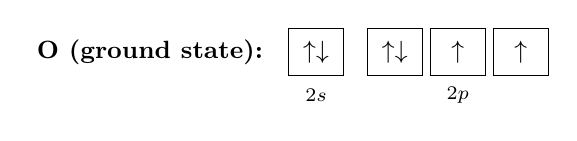
\begin{tikzpicture}[every node/.style={font=\small}]
  \node[anchor=east] at (-0.2, 0) {\textbf{O (ground state):}};
  % 2s
  \draw (0,-0.3) rectangle (0.7,0.3);
  \node at (0.35,0.0) {$\uparrow\downarrow$};
  \node[font=\scriptsize] at (0.35,-0.55) {$2s$};
  % 2p
  \foreach \x/\c in {1.0/$\uparrow\downarrow$, 1.8/$\uparrow$, 2.6/$\uparrow$}{
    \draw (\x,-0.3) rectangle (\x+0.7,0.3);
    \node at (\x+0.35,0.0) {\c};
  }
  \node[font=\scriptsize] at (2.15,-0.55) {$2p$};
\end{tikzpicture}
\end{center}

O has 2 half-filled $2p$ orbitals $\Rightarrow$ pure VBT predicts bond angle $= 90^\circ$,
but observed angle is $104.5^\circ$. So hybridization must occur.

\medskip
\textbf{Step 2: Hybridization --- mixing of $2s$ and three $2p$ orbitals}

\begin{center}
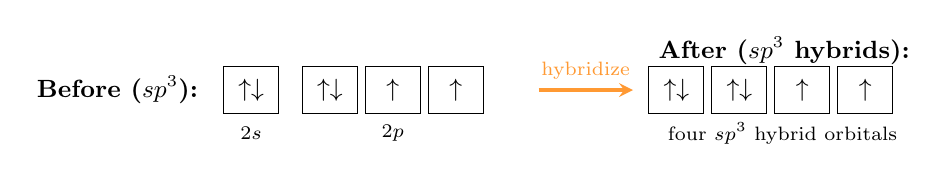
\begin{tikzpicture}[every node/.style={font=\small}, >=stealth]
  % Before hybridization
  \node[anchor=east] at (-0.2, 0) {\textbf{Before ($sp^3$):}};
  \draw (0,-0.3) rectangle (0.7,0.3); \node at (0.35,0) {$\uparrow\downarrow$};
  \node[font=\scriptsize] at (0.35,-0.55) {$2s$};
  \foreach \x/\c in {1.0/$\uparrow\downarrow$,1.8/$\uparrow$,2.6/$\uparrow$}{
    \draw (\x,-0.3) rectangle (\x+0.7,0.3);
    \node at (\x+0.35,0) {\c};
  }
  \node[font=\scriptsize] at (2.15,-0.55) {$2p$};

  % Arrow
  \draw[->,very thick,orange!80] (4.0,0) -- (5.2,0)
        node[midway,above,font=\scriptsize]{hybridize};

  % After hybridization
  \node[anchor=west] at (5.4, 0.5) {\textbf{After ($sp^3$ hybrids):}};
  \foreach \x/\c in {5.4/$\uparrow\downarrow$,6.2/$\uparrow\downarrow$,
                      7.0/$\uparrow$,7.8/$\uparrow$}{
    \draw (\x,-0.3) rectangle (\x+0.7,0.3);
    \node at (\x+0.35,0) {\c};
  }
  \node[font=\scriptsize] at (7.1,-0.55) {four $sp^3$ hybrid orbitals};
\end{tikzpicture}
\end{center}

\begin{itemize}[itemsep=3pt]
  \item $2s + 2p_x + 2p_y + 2p_z$ mix to give \textbf{four $sp^3$ hybrid orbitals}.
  \item \textbf{2 hybrid orbitals} contain lone pairs (LP).
  \item \textbf{2 hybrid orbitals} are half-filled $\Rightarrow$ overlap with $1s$
        orbitals of two H atoms to form \textbf{2 O--H $\sigma$ bonds}.
\end{itemize}

\medskip\begin{center}
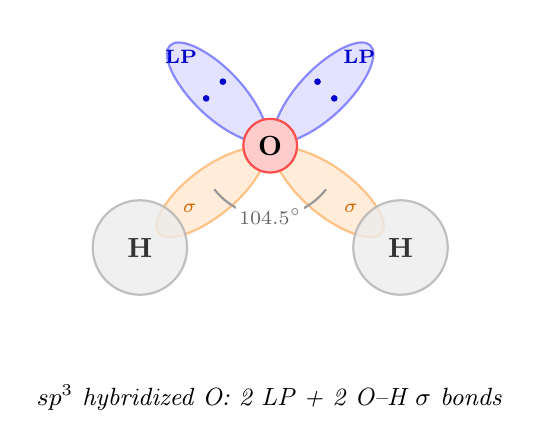
\begin{tikzpicture}[every node/.style={font=\small}, >=stealth]

  % Define a reusable command for drawing perfect symmetrical sp3 lobes
  \def\lobe#1#2#3{
    \filldraw[rotate=#1, fill=#2, draw=#3, thick, opacity=0.75] 
      (0,0) .. controls (0.6, 0.5) and (1.8, 0.3) .. (1.8, 0) 
            .. controls (1.8,-0.3) and (0.6,-0.5) .. (0,0);
  }

  % 1. Draw Lone Pair Lobes (Top)
  \lobe{135}{blue!15}{blue!60}
  \lobe{45}{blue!15}{blue!60}
  
  % Lone pair labels & electrons (dots)
  \node[font=\scriptsize\bfseries, blue!80!black] at (135:1.6) {LP};
  \node[font=\scriptsize\bfseries, blue!80!black] at (45:1.6) {LP};
  \fill[rotate=135, blue!80!black] (1.0, 0.15) circle (1.2pt);
  \fill[rotate=135, blue!80!black] (1.0,-0.15) circle (1.2pt);
  \fill[rotate=45, blue!80!black] (1.0, 0.15) circle (1.2pt);
  \fill[rotate=45, blue!80!black] (1.0,-0.15) circle (1.2pt);

  % 2. Draw Bonding Lobes (Bottom) pointing toward H
  % Water bond angle is 104.5 degrees. (270 +/- 52.25) => 218 and 322
  \lobe{218}{orange!20}{orange!60}
  \lobe{322}{orange!20}{orange!60}

  % 3. Draw H 1s orbitals (spheres overlapping the orange lobes)
  \filldraw[fill=gray!15, draw=gray!60, thick, opacity=0.8] (218:2.1) circle (0.6cm);
  \filldraw[fill=gray!15, draw=gray!60, thick, opacity=0.8] (322:2.1) circle (0.6cm);

  % Atom Labels
  \node[circle, fill=red!20, draw=red!70, thick, inner sep=3pt, font=\bfseries] (O) at (0,0) {O};
  \node[font=\bfseries, text=black!80] at (218:2.1) {H};
  \node[font=\bfseries, text=black!80] at (322:2.1) {H};

  % Sigma bond labels (placed at the overlap region)
  \node[font=\scriptsize\bfseries, orange!80!black] at (218:1.3) {$\sigma$};
  \node[font=\scriptsize\bfseries, orange!80!black] at (322:1.3) {$\sigma$};

  % Bond angle arc
  \draw[thick, gray!80] (218:0.9) arc[start angle=218, end angle=322, radius=0.9cm];
  \node[font=\scriptsize\bfseries, gray!80!black, fill=white, inner sep=1pt] at (270:0.9) {$104.5^\circ$};

  % Caption
  \node at (0,-3.2) {\textit{$sp^3$ hybridized O: 2 LP + 2 O--H $\sigma$ bonds}};

\end{tikzpicture}
\end{center}
\medskip
\textbf{Step 4: Why bond angle is $104.5^\circ$ and not $109.5^\circ$}

\begin{itemize}[itemsep=3pt]
  \item Perfect tetrahedral $sp^3$ predicts $109.5^\circ$, but in H$_2$O there are
        \textbf{2 lone pairs} which exert stronger repulsion than bonding pairs.
  \item LP--LP $>$ LP--BP $>$ BP--BP repulsion compresses the H--O--H angle
        from $109.5^\circ$ down to $\mathbf{104.5^\circ}$.
\end{itemize}

\begin{center}
\renewcommand{\arraystretch}{1.4}
\begin{tabular}{ll}
\toprule
\textbf{Property}        & \textbf{Value}\\
\midrule
Central atom             & O\\
Hybridization            & $sp^3$\\
Bonding pairs            & 2\\
Lone pairs               & 2\\
Electron geometry        & Tetrahedral\\
Molecular shape          & Bent / V-shaped\\
Bond angle               & $104.5^\circ$\\
Bond type                & O--H $\sigma$ (overlap of $sp^3$ and $1s$)\\
\bottomrule
\end{tabular}
\end{center}

\end{tcolorbox}

\item Use the VSEPR model to predict the geometry of the following ions: (i) N$_3^-$ (ii) BH$_4^-$ (iii) SO$_3^{2-}$ (iv) NO$_2^-$. \mk{8}
\yr{CHEM 113 | 2015--16}

\begin{tcolorbox}[enhanced,breakable,ansbox,colback=cB!4,colframe=cB,boxrule=0.8pt,arc=5pt,title={\textbf{Answer}},fonttitle=\bfseries\color{white},colbacktitle=cB]
\textbf{Using VSEPR Theory} --- Total electron pairs (BP + LP) determine geometry.

\medskip
%---------------------------------------------------------
\textbf{(i) N$_3^-$ (Azide ion)}
%---------------------------------------------------------

\begin{itemize}[itemsep=2pt]
  \item Valence electrons: $3\times5 + 1 = 16$ electrons
  \item Central N is double-bonded to both terminal N atoms: \textbf{linear arrangement}
  \item BP $= 2$, LP $= 1$ on central N (but linear due to resonance/triple bond character)
  \item \textbf{Geometry: Linear}, bond angle $= 180^\circ$
\end{itemize}

\[
\left[
\chemfig{
  \charge{180=\:, 90=\:}{N}
  =[0]
  N
  =[0]
  \charge{0=\:,270=\:}{N}
}  \right]^-
\]

\medskip
%---------------------------------------------------------
\textbf{(ii) BH$_4^-$ (Tetrahydroborate ion)}
%---------------------------------------------------------

\begin{itemize}[itemsep=2pt]
  \item Valence electrons: $3 + 4\times1 + 1 = 8$ electrons
  \item B is the central atom bonded to 4 H atoms
  \item BP $= 4$, LP $= 0$
  \item \textbf{Geometry: Tetrahedral}, bond angle $= 109.5^\circ$
\end{itemize}


\[ 
\left[ \chemfig{B(-[:210]H)(<:[:330]H)(<[:300]H)(-[:90]H)} \right]^{-}
\]

\medskip
%---------------------------------------------------------
\textbf{(iii) SO$_3^{2-}$ (Sulphite ion)}
%---------------------------------------------------------

\begin{itemize}[itemsep=2pt]
  \item Valence electrons: $6 + 3\times6 + 2 = 26$ electrons
  \item S is the central atom bonded to 3 O atoms; 1 LP on S
  \item BP $= 3$, LP $= 1$ $\Rightarrow$ electron geometry: Tetrahedral
  \item \textbf{Geometry: Trigonal Pyramidal}, bond angle $\approx 106^\circ$
\end{itemize}

\[
\chemleft[
  \chemfig{
    \charge{90=\:}{S} % সালফারের উপর লোন পেয়ার (|)
    ( =[:210]O )
    ( -[:330]O )
    ( -[:300]O )
  }
\chemright]^{2-}
\]

\medskip
%---------------------------------------------------------
\textbf{(iv) NO$_2^-$ (Nitrite ion)}
%---------------------------------------------------------

\begin{itemize}[itemsep=2pt]
  \item Valence electrons: $5 + 2\times6 + 1 = 18$ electrons
  \item N is the central atom bonded to 2 O atoms; 1 LP on N
  \item BP $= 2$, LP $= 1$ $\Rightarrow$ electron geometry: Trigonal Planar
  \item \textbf{Geometry: Bent (V-shaped)}, bond angle $\approx 115^\circ$
\end{itemize}

\begin{center}
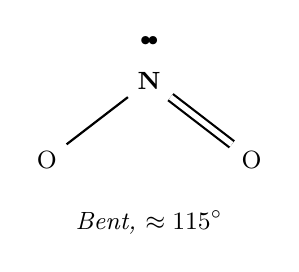
\begin{tikzpicture}[every node/.style={font=\small}]
  \node (N)  at ( 0,   0  ) {\textbf{N}};
  \node (O1) at (-1.3,-1.0) {O};
  \node (O2) at ( 1.3,-1.0) {O};
  \draw[thick] (N) -- (O1);
  \draw[thick, double distance=2pt] (N) -- (O2);
  \node[font=\scriptsize] at (0, 0.5) {$\bullet\!\bullet$};
  \node at (0,-1.8) {\textit{Bent, $\approx 115^\circ$}};
\end{tikzpicture}
\end{center}

\end{tcolorbox}

\item In the trigonal bipyramidal arrangement for a system AB$_4$E, why does the lone pair occupy an equatorial position rather than an axial position? Sketch the bond moments and resultant dipole moments for the following molecules: H$_2$O, PCl$_3$, XeF$_4$, PCl$_5$, SF$_6$. \mk{12}
\yr{CHEM 113 | 2014--15}
\begin{tcolorbox}[enhanced,breakable,ansbox,colback=cB!4,colframe=cB,boxrule=0.8pt,arc=5pt,title={\textbf{Answer}},fonttitle=\bfseries\color{white},colbacktitle=cB]

%---------------------------------------------------------
\textbf{Part 1: Why lone pair occupies equatorial position in AB$_4$E}
%---------------------------------------------------------

In a trigonal bipyramidal system, an \textbf{equatorial lone pair} experiences fewer repulsions than an axial lone pair:

\begin{center}
\renewcommand{\arraystretch}{1.4}
\begin{tabularx}{\linewidth}{lXXl}
\toprule
\textbf{LP Position} & \textbf{$90^\circ$ LP--BP interactions} & \textbf{$120^\circ$ LP--BP interactions} & \textbf{Stability}\\
\midrule
Axial       & 3 & 0 & Less stable\\
Equatorial  & 2 & 2 & \textbf{More stable} $\checkmark$\\
\bottomrule
\end{tabularx}
\end{center}

\begin{itemize}[itemsep=3pt, label=\textcolor{cB}{$\bullet$}]
  \item LP--BP repulsion at $90^\circ$ is very strong; minimizing these interactions lowers energy.
  \item An \textbf{axial} LP has $3$ interactions at $90^\circ$ with equatorial BPs.
  \item An \textbf{equatorial} LP has only $2$ interactions at $90^\circ$ with axial BPs.
  \item Equatorial positions also have more angular space ($120^\circ$ separation) to accommodate the diffuse lone pair cloud.
  \item Therefore the lone pair always prefers the \textbf{equatorial position} $\Rightarrow$ giving AB$_4$E a \textbf{see-saw shape}.
\end{itemize}

\medskip
%---------------------------------------------------------
\textbf{Part 2: Bond moments and resultant dipole moments}
%---------------------------------------------------------

\medskip
%--- H2O --------------------------------------------------
\textbf{(i) H$_2$O} \hfill \textit{Bent, $sp^3$, \textbf{Net dipole $\neq 0$}}

\begin{itemize}[itemsep=2pt, label=\textcolor{cB}{$\bullet$}]
  \item O is more electronegative than H $\Rightarrow$ bond moments point \textbf{toward O}.
  \item Two O--H bond moments add up (do not cancel) due to bent geometry.
  \item \textbf{Resultant dipole moment is non-zero}, pointing from H--H midpoint toward O.
\end{itemize}

\begin{center}
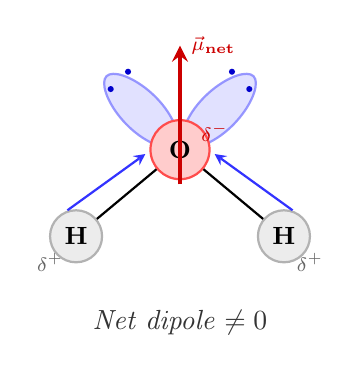
\begin{tikzpicture}[>=stealth, font=\small, scale=1.1]
  % LP Lobes
  \filldraw[rotate=135, fill=blue!15, draw=blue!50, thick, opacity=0.8] 
    (0,0) .. controls (0.4,0.4) and (1.2,0.2) .. (1.2,0) .. controls (1.2,-0.2) and (0.4,-0.4) .. (0,0);
  \filldraw[rotate=45, fill=blue!15, draw=blue!50, thick, opacity=0.8] 
    (0,0) .. controls (0.4,0.4) and (1.2,0.2) .. (1.2,0) .. controls (1.2,-0.2) and (0.4,-0.4) .. (0,0);
  \fill[blue!80!black] (-0.8, 0.7) circle (1pt); \fill[blue!80!black] (-0.6, 0.9) circle (1pt);
  \fill[blue!80!black] ( 0.8, 0.7) circle (1pt); \fill[blue!80!black] ( 0.6, 0.9) circle (1pt);

  % Bonds & Atoms
  \draw[thick] (0,0) -- (-1.2,-1.0);
  \draw[thick] (0,0) -- ( 1.2,-1.0);
  \node[circle, fill=red!20, draw=red!70, thick, inner sep=4pt] (O) at (0,0) {\textbf{O}};
  \node[circle, fill=gray!15, draw=gray!60, thick, inner sep=3pt] (H1) at (-1.2,-1.0) {\textbf{H}};
  \node[circle, fill=gray!15, draw=gray!60, thick, inner sep=3pt] (H2) at ( 1.2,-1.0) {\textbf{H}};

  % Bond Moments
  \draw[->, thick, blue!80] (-1.3,-0.7) -- (-0.4,-0.05);
  \draw[->, thick, blue!80] ( 1.3,-0.7) -- ( 0.4,-0.05);

  % Resultant Dipole
  \draw[->, line width=1.5pt, red!80!black] (0,-0.4) -- (0, 1.2) node[right, font=\scriptsize\bfseries] {$\vec{\mu}_{\text{net}}$};

  % Labels
  \node[font=\scriptsize\bfseries, gray!80!black] at (-1.5, -1.3) {$\delta^+$};
  \node[font=\scriptsize\bfseries, gray!80!black] at ( 1.5, -1.3) {$\delta^+$};
  \node[font=\scriptsize\bfseries, red!80!black]  at ( 0.4,  0.2) {$\delta^-$};
  \node[font=\itshape, text=black!80] at (0,-2.0) {Net dipole $\neq 0$};
\end{tikzpicture}
\end{center}

\medskip
%--- PCl3 -------------------------------------------------
\textbf{(ii) PCl$_3$} \hfill \textit{Trigonal Pyramidal, $sp^3$, \textbf{Net dipole $\neq 0$}}

\begin{itemize}[itemsep=2pt, label=\textcolor{cB}{$\bullet$}]
  \item Cl is more electronegative than P $\Rightarrow$ bond moments point \textbf{toward Cl}.
  \item 1 LP on P adds to the net moment in the same direction.
  \item Three P--Cl bond moments do \textbf{not} cancel $\Rightarrow$ resultant points downward.
  \item \textbf{Net dipole moment $\neq 0$}.
\end{itemize}

\begin{center}
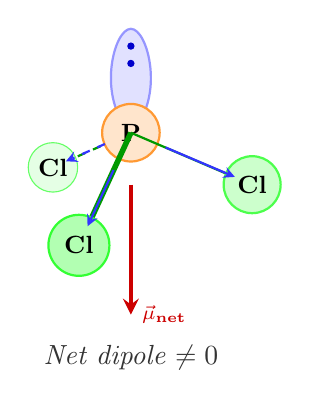
\begin{tikzpicture}[>=stealth, font=\small, scale=1.1]
  % LP Lobe (Top)
  \filldraw[rotate=90, fill=blue!15, draw=blue!50, thick, opacity=0.8] 
    (0,0) .. controls (0.4,0.4) and (1.2,0.2) .. (1.2,0) .. controls (1.2,-0.2) and (0.4,-0.4) .. (0,0);
  \fill[blue!80!black] (0, 0.8) circle (1.2pt); \fill[blue!80!black] (0, 1.0) circle (1.2pt);

  % Back Bond (Dashed) - Pointing down-left
  \draw[thick, dashed, green!60!black] (0,0) -- (-0.9, -0.4);
  \node[circle, fill=green!10, draw=green!60, inner sep=2pt] at (-0.9, -0.4) {\textbf{Cl}};

  % Central P Atom
  \node[circle, fill=orange!20, draw=orange!80, thick, inner sep=4pt] (P) at (0,0) {\textbf{P}};

  % Right Bond (Solid, in-plane)
  \draw[thick, green!60!black] (0,0) -- ( 1.4, -0.6);
  \node[circle, fill=green!20, draw=green!70, thick, inner sep=3pt] at ( 1.4, -0.6) {\textbf{Cl}};

  % Front Bond (Wedge) - Pointing down-left
  \draw[line width=2pt, green!60!black] (0,0) -- (-0.6, -1.3);
  \node[circle, fill=green!30, draw=green!80, thick, inner sep=3.5pt] at (-0.6, -1.3) {\textbf{Cl}};

  % Bond Moments (Blue arrows)
  \draw[->, thick, blue!80, dashed] (-0.3, -0.13) -- (-0.75, -0.33); % Back
  \draw[->, thick, blue!80] ( 0.4, -0.17) -- ( 1.2, -0.51); % Right
  \draw[->, thick, blue!80] (-0.2, -0.43) -- (-0.5, -1.08); % Front

  % Resultant Dipole (Red arrow)
  \draw[->, line width=1.5pt, red!80!black] (0, -0.6) -- (0, -2.1) node[right, font=\scriptsize\bfseries] {$\vec{\mu}_{\text{net}}$};
  
  \node[font=\itshape, text=black!80] at (0,-2.6) {Net dipole $\neq 0$};
\end{tikzpicture}
\end{center}

\medskip
%--- XeF4 -------------------------------------------------
\textbf{(iii) XeF$_4$} \hfill \textit{Square Planar, $sp^3d^2$, \textbf{Net dipole $= 0$}}

\begin{itemize}[itemsep=2pt, label=\textcolor{cB}{$\bullet$}]
  \item Xe has 2 LP occupying axial positions (opposite each other).
  \item 4 Xe--F bond moments point toward F (in the equatorial plane).
  \item Opposite bond moments \textbf{cancel in pairs} $\Rightarrow$ net bond moment $= 0$.
  \item Two axial LP moments also cancel each other.
  \item \textbf{Net dipole moment $= 0$}.
\end{itemize}

\begin{center}
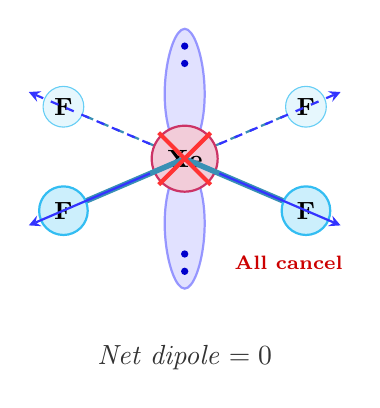
\begin{tikzpicture}[>=stealth, font=\small, scale=1.1]
  % Define a macro for lobes
  \def\lobe#1{
    \filldraw[rotate=#1, fill=blue!15, draw=blue!50, thick, opacity=0.8] 
      (0,0) .. controls (0.4,0.4) and (1.5,0.2) .. (1.5,0) .. controls (1.5,-0.2) and (0.4,-0.4) .. (0,0);
  }
  
  % Back Bonds
  \draw[thick, dashed, cyan!70!black] (0,0) -- (-1.4, 0.6);
  \draw[thick, dashed, cyan!70!black] (0,0) -- ( 1.4, 0.6);
  \node[circle, fill=cyan!10, draw=cyan!60, inner sep=2pt] at (-1.4, 0.6) {\textbf{F}};
  \node[circle, fill=cyan!10, draw=cyan!60, inner sep=2pt] at ( 1.4, 0.6) {\textbf{F}};

  % LP Lobes (Axial)
  \lobe{90} \fill[blue!80!black] (0, 1.1) circle (1.2pt); \fill[blue!80!black] (0, 1.3) circle (1.2pt);
  \lobe{270} \fill[blue!80!black] (0,-1.1) circle (1.2pt); \fill[blue!80!black] (0,-1.3) circle (1.2pt);

  % Central Atom
  \node[circle, fill=purple!20, draw=purple!80, thick, inner sep=3.5pt] (Xe) at (0,0) {\textbf{Xe}};

  % Front Bonds (Wedges)
  \draw[line width=2pt, cyan!70!black] (0,0) -- (-1.4,-0.6);
  \draw[line width=2pt, cyan!70!black] (0,0) -- ( 1.4,-0.6);
  \node[circle, fill=cyan!20, draw=cyan!80, thick, inner sep=3pt] at (-1.4,-0.6) {\textbf{F}};
  \node[circle, fill=cyan!20, draw=cyan!80, thick, inner sep=3pt] at ( 1.4,-0.6) {\textbf{F}};

  % Bond Moments
  \draw[->, thick, blue!80] (-0.4,-0.17) -- (-1.8,-0.77);
  \draw[->, thick, blue!80] ( 0.4,-0.17) -- ( 1.8,-0.77);
  \draw[->, thick, blue!80, dashed] (-0.4, 0.17) -- (-1.8, 0.77);
  \draw[->, thick, blue!80, dashed] ( 0.4, 0.17) -- ( 1.8, 0.77);

  % Cancel Indicator
  \draw[red!80, line width=1.5pt] (-0.3,-0.3) -- (0.3,0.3);
  \draw[red!80, line width=1.5pt] (-0.3, 0.3) -- (0.3,-0.3);
  \node[font=\scriptsize\bfseries, red!80!black] at (1.2, -1.2) {All cancel};

  \node[font=\itshape, text=black!80] at (0,-2.3) {Net dipole $= 0$};
\end{tikzpicture}
\end{center}

\medskip
%--- PCl5 -------------------------------------------------
\textbf{(iv) PCl$_5$} \hfill \textit{Trigonal Bipyramidal, $sp^3d$, \textbf{Net dipole $= 0$}}

\begin{itemize}[itemsep=2pt, label=\textcolor{cB}{$\bullet$}]
  \item 2 axial P--Cl bond moments are equal and \textbf{opposite} $\Rightarrow$ cancel.
  \item 3 equatorial P--Cl bond moments are symmetric at $120^\circ$ $\Rightarrow$ cancel.
  \item \textbf{Net dipole moment $= 0$}.
\end{itemize}

\begin{center}
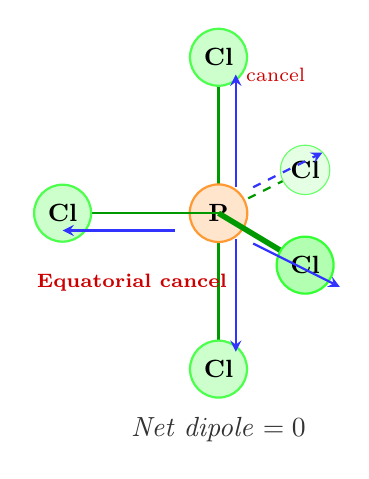
\begin{tikzpicture}[>=stealth, font=\small, scale=1.1]
  % Back Equatorial Bond
  \draw[thick, dashed, green!60!black] (0,0) -- (1.0, 0.5);
  \node[circle, fill=green!10, draw=green!60, inner sep=2pt] at (1.0, 0.5) {\textbf{Cl}};

  % Axial Bonds
  \draw[thick, green!60!black] (0,0) -- (0, 1.8);
  \draw[thick, green!60!black] (0,0) -- (0,-1.8);
  \node[circle, fill=green!20, draw=green!70, thick, inner sep=3pt] at (0, 1.8) {\textbf{Cl}};
  \node[circle, fill=green!20, draw=green!70, thick, inner sep=3pt] at (0,-1.8) {\textbf{Cl}};

  % Central Atom
  \node[circle, fill=orange!20, draw=orange!80, thick, inner sep=4pt] (P) at (0,0) {\textbf{P}};

  % Left Equatorial Bond
  \draw[thick, green!60!black] (0,0) -- (-1.8, 0);
  \node[circle, fill=green!20, draw=green!70, thick, inner sep=3pt] at (-1.8, 0) {\textbf{Cl}};

  % Front Right Equatorial Bond (Wedge)
  \draw[line width=2pt, green!60!black] (0,0) -- (1.0, -0.6);
  \node[circle, fill=green!30, draw=green!80, thick, inner sep=3pt] at (1.0, -0.6) {\textbf{Cl}};

  % Bond Moments
  \draw[->, thick, blue!80] (0.2, 0.3) -- (0.2, 1.6) node[right, font=\scriptsize, red!80!black] {cancel};
  \draw[->, thick, blue!80] (0.2,-0.3) -- (0.2,-1.6);
  \draw[->, thick, blue!80] (-0.5, -0.2) -- (-1.8, -0.2);
  \draw[->, thick, blue!80] (0.4, -0.35) -- (1.4, -0.85);
  \draw[->, thick, blue!80, dashed] (0.4, 0.3) -- (1.2, 0.7);

  \node[font=\scriptsize\bfseries, red!80!black] at (-1.0, -0.8) {Equatorial cancel};
  \node[font=\itshape, text=black!80] at (0,-2.5) {Net dipole $= 0$};
\end{tikzpicture}
\end{center}

\medskip
%--- SF6 --------------------------------------------------
\textbf{(v) SF$_6$} \hfill \textit{Octahedral, $sp^3d^2$, \textbf{Net dipole $= 0$}}

\begin{itemize}[itemsep=2pt, label=\textcolor{cB}{$\bullet$}]
  \item 6 S--F bond moments arranged symmetrically along $\pm x$, $\pm y$, $\pm z$ axes.
  \item Every bond moment is cancelled by the equal and opposite bond moment.
  \item \textbf{Net dipole moment $= 0$}.
\end{itemize}

\begin{center}
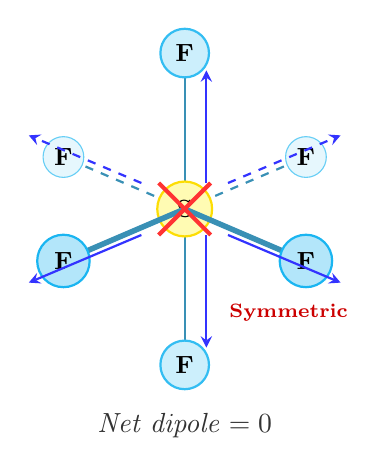
\begin{tikzpicture}[>=stealth, font=\small, scale=1.1]
  % Back Equatorial Bonds
  \draw[thick, dashed, cyan!70!black] (0,0) -- (-1.4, 0.6);
  \draw[thick, dashed, cyan!70!black] (0,0) -- ( 1.4, 0.6);
  \node[circle, fill=cyan!10, draw=cyan!60, inner sep=2pt] at (-1.4, 0.6) {\textbf{F}};
  \node[circle, fill=cyan!10, draw=cyan!60, inner sep=2pt] at ( 1.4, 0.6) {\textbf{F}};

  % Axial Bonds
  \draw[thick, cyan!70!black] (0,0) -- (0, 1.8);
  \draw[thick, cyan!70!black] (0,0) -- (0,-1.8);
  \node[circle, fill=cyan!20, draw=cyan!80, thick, inner sep=3pt] at (0, 1.8) {\textbf{F}};
  \node[circle, fill=cyan!20, draw=cyan!80, thick, inner sep=3pt] at (0,-1.8) {\textbf{F}};

  % Central Atom
  \node[circle, fill=yellow!30, draw=yellow!80!orange, thick, inner sep=4pt] (S) at (0,0) {\textbf{S}};

  % Front Equatorial Bonds (Wedges)
  \draw[line width=2pt, cyan!70!black] (0,0) -- (-1.4,-0.6);
  \draw[line width=2pt, cyan!70!black] (0,0) -- ( 1.4,-0.6);
  \node[circle, fill=cyan!30, draw=cyan!90, thick, inner sep=3.5pt] at (-1.4,-0.6) {\textbf{F}};
  \node[circle, fill=cyan!30, draw=cyan!90, thick, inner sep=3.5pt] at ( 1.4,-0.6) {\textbf{F}};

  % Bond Moments
  \draw[->, thick, blue!80] (0.25, 0.3) -- (0.25, 1.6);
  \draw[->, thick, blue!80] (0.25,-0.3) -- (0.25,-1.6);
  \draw[->, thick, blue!80] (-0.5,-0.3) -- (-1.8,-0.85);
  \draw[->, thick, blue!80] ( 0.5,-0.3) -- ( 1.8,-0.85);
  \draw[->, thick, blue!80, dashed] (-0.5, 0.3) -- (-1.8, 0.85);
  \draw[->, thick, blue!80, dashed] ( 0.5, 0.3) -- ( 1.8, 0.85);

  % Cancel Indicator
  \draw[red!80, line width=1.5pt] (-0.3,-0.3) -- (0.3,0.3);
  \draw[red!80, line width=1.5pt] (-0.3, 0.3) -- (0.3,-0.3);
  \node[font=\scriptsize\bfseries, red!80!black] at (1.2, -1.2) {Symmetric};
  \node[font=\itshape, text=black!80] at (0,-2.5) {Net dipole $= 0$};
\end{tikzpicture}
\end{center}

\medskip
\begin{center}
\renewcommand{\arraystretch}{1.4}
\begin{tabular}{llccl}
\toprule
\textbf{Molecule} & \textbf{Shape} & \textbf{Hybrid} & \textbf{Dipole Moment}\\
\midrule
H$_2$O   & Bent                  & $sp^3$     & $\neq 0$ (polar)\\
PCl$_3$  & Trigonal Pyramidal    & $sp^3$     & $\neq 0$ (polar)\\
XeF$_4$  & Square Planar         & $sp^3d^2$  & $= 0$ (non-polar)\\
PCl$_5$  & Trigonal Bipyramidal  & $sp^3d$    & $= 0$ (non-polar)\\
SF$_6$   & Octahedral            & $sp^3d^2$  & $= 0$ (non-polar)\\
\bottomrule
\end{tabular}
\end{center}

\end{tcolorbox}
\item Discuss the shapes of the following molecules: H$_2$O, NH$_3$, BaCl$_2$, CH$_4$. \mk{8}
\yr{CHEM 113 | 2013--14}
\begin{tcolorbox}[enhanced,breakable,ansbox,colback=cB!4,colframe=cB,boxrule=0.8pt,arc=5pt,title={\textbf{Answer}},fonttitle=\bfseries\color{white},colbacktitle=cB]

%---------------------------------------------------------
\textbf{(i) H$_2$O (Water)}
%---------------------------------------------------------

\begin{itemize}[itemsep=2pt, label=\textcolor{cB}{$\bullet$}]
  \item \textbf{Valence electrons:} $6 + 2\times1 = 8$ electrons
  \item O is the central atom bonded to 2 H atoms; \textbf{2 LP} on O
  \item BP $= 2$, LP $= 2$ $\Rightarrow$ Total electron pairs $= 4$
  \item \textbf{Hybridization:} $sp^3$
  \item Electron geometry: Tetrahedral
  \item \textbf{Shape: Bent (V-shaped)}, bond angle $\approx 104.5^\circ$\\
        (reduced from $109.5^\circ$ due to strong LP--LP and LP--BP repulsions)
\end{itemize}

\begin{center}
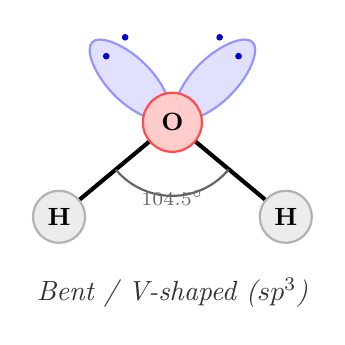
\begin{tikzpicture}[>=stealth, scale=1.2, font=\small]
  % LP Lobes
  \filldraw[rotate=135, fill=blue!15, draw=blue!50, thick, opacity=0.8] 
    (0,0) .. controls (0.4,0.4) and (1.2,0.2) .. (1.2,0) .. controls (1.2,-0.2) and (0.4,-0.4) .. (0,0);
  \filldraw[rotate=45, fill=blue!15, draw=blue!50, thick, opacity=0.8] 
    (0,0) .. controls (0.4,0.4) and (1.2,0.2) .. (1.2,0) .. controls (1.2,-0.2) and (0.4,-0.4) .. (0,0);
  \fill[blue!80!black] (-0.7, 0.7) circle (1pt); \fill[blue!80!black] (-0.5, 0.9) circle (1pt);
  \fill[blue!80!black] ( 0.7, 0.7) circle (1pt); \fill[blue!80!black] ( 0.5, 0.9) circle (1pt);

  % Bonds
  \draw[line width=1.5pt] (0,0) -- (-1.2,-1.0);
  \draw[line width=1.5pt] (0,0) -- ( 1.2,-1.0);

  % Atoms
  \node[circle, fill=red!20, draw=red!70, thick, inner sep=4pt] (O) at (0,0) {\textbf{O}};
  \node[circle, fill=gray!15, draw=gray!60, thick, inner sep=3pt] at (-1.2,-1.0) {\textbf{H}};
  \node[circle, fill=gray!15, draw=gray!60, thick, inner sep=3pt] at ( 1.2,-1.0) {\textbf{H}};

  % Angle arc
  \draw[thick, gray!80!black] (-0.6,-0.5) arc[start angle=220, end angle=320, radius=0.78cm];
  \node[font=\scriptsize\bfseries, gray!80!black] at (0,-0.8) {$104.5^\circ$};

  \node[font=\itshape, text=black!80] at (0,-1.8) {Bent / V-shaped ($sp^3$)};
\end{tikzpicture}
\end{center}

\medskip
%---------------------------------------------------------
\textbf{(ii) NH$_3$ (Ammonia)}
%---------------------------------------------------------

\begin{itemize}[itemsep=2pt, label=\textcolor{cB}{$\bullet$}]
  \item \textbf{Valence electrons:} $5 + 3\times1 = 8$ electrons
  \item N is the central atom bonded to 3 H atoms; \textbf{1 LP} on N
  \item BP $= 3$, LP $= 1$ $\Rightarrow$ Total electron pairs $= 4$
  \item \textbf{Hybridization:} $sp^3$
  \item Electron geometry: Tetrahedral
  \item \textbf{Shape: Trigonal Pyramidal}, bond angle $\approx 107^\circ$\\
        (reduced from $109.5^\circ$ due to LP--BP repulsion)
\end{itemize}

\begin{center}
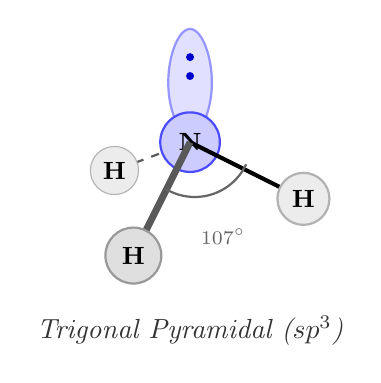
\begin{tikzpicture}[>=stealth, scale=1.2, font=\small]
  % LP Lobe
  \filldraw[rotate=90, fill=blue!15, draw=blue!50, thick, opacity=0.8] 
    (0,0) .. controls (0.4,0.4) and (1.2,0.2) .. (1.2,0) .. controls (1.2,-0.2) and (0.4,-0.4) .. (0,0);
  \fill[blue!80!black] (0, 0.7) circle (1.2pt); \fill[blue!80!black] (0, 0.9) circle (1.2pt);

  % Back Bond (Dashed)
  \draw[thick, dashed, gray!70!black] (0,0) -- (-0.8,-0.3);
  \node[circle, fill=gray!15, draw=gray!60, inner sep=2.5pt] at (-0.8,-0.3) {\textbf{H}};

  % Central Atom
  \node[circle, fill=blue!20, draw=blue!70, thick, inner sep=4pt] (N) at (0,0) {\textbf{N}};

  % Right Bond (Solid)
  \draw[line width=1.5pt] (0,0) -- ( 1.2,-0.6);
  \node[circle, fill=gray!15, draw=gray!60, thick, inner sep=3pt] at ( 1.2,-0.6) {\textbf{H}};

  % Front Bond (Wedge)
  \draw[line width=2.5pt, gray!70!black] (0,0) -- (-0.6,-1.2);
  \node[circle, fill=gray!25, draw=gray!80, thick, inner sep=3.5pt] at (-0.6,-1.2) {\textbf{H}};

  % Angle arc
  \draw[thick, gray!80!black] (-0.25,-0.5) arc[start angle=240, end angle=335, radius=0.6cm];
  \node[font=\scriptsize\bfseries, gray!80!black] at (0.35,-1.0) {$107^\circ$};

  \node[font=\itshape, text=black!80] at (0,-2.0) {Trigonal Pyramidal ($sp^3$)};
\end{tikzpicture}
\end{center}

\medskip
%---------------------------------------------------------
\textbf{(iii) BaCl$_2$ (Barium Chloride)}
%---------------------------------------------------------

\begin{itemize}[itemsep=2pt, label=\textcolor{cB}{$\bullet$}]
  \item \textbf{Valence electrons:} $2 + 2\times7 = 16$ electrons
  \item Ba is the central atom bonded to 2 Cl atoms; \textbf{0 LP} on Ba
  \item BP $= 2$, LP $= 0$ $\Rightarrow$ Total electron pairs $= 2$
  \item \textbf{Hybridization:} $sp$
  \item Electron geometry $=$ Molecular geometry
  \item \textbf{Shape: Linear}, bond angle $= 180^\circ$
\end{itemize}

\begin{center}
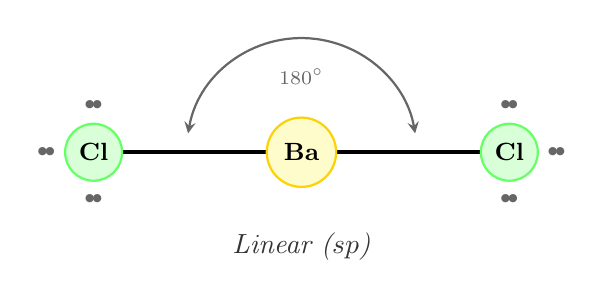
\begin{tikzpicture}[>=stealth, scale=1.2, font=\small]
  % Bonds
  \draw[line width=1.5pt] (-2.2,0) -- (2.2,0);

  % Atoms
  \node[circle, fill=green!15, draw=green!60, thick, inner sep=3pt] at (-2.2,0) {\textbf{Cl}};
  \node[circle, fill=green!15, draw=green!60, thick, inner sep=3pt] at ( 2.2,0) {\textbf{Cl}};
  \node[circle, fill=yellow!20, draw=yellow!70!orange, thick, inner sep=4pt] at (0,0) {\textbf{Ba}};

  % Lone Pairs on Cl
  \node[font=\scriptsize, gray!80!black] at (-2.2, 0.5) {$\bullet\!\bullet$};
  \node[font=\scriptsize, gray!80!black] at (-2.2,-0.5) {$\bullet\!\bullet$};
  \node[font=\scriptsize, gray!80!black] at (-2.7, 0)   {$\bullet\!\bullet$};
  \node[font=\scriptsize, gray!80!black] at ( 2.2, 0.5) {$\bullet\!\bullet$};
  \node[font=\scriptsize, gray!80!black] at ( 2.2,-0.5) {$\bullet\!\bullet$};
  \node[font=\scriptsize, gray!80!black] at ( 2.7, 0)   {$\bullet\!\bullet$};

  % Angle arc
  \draw[<->, thick, gray!80!black] (-1.2, 0.2) arc[start angle=170, end angle=10, radius=1.22cm];
  \node[font=\scriptsize\bfseries, gray!80!black] at (0, 0.8) {$180^\circ$};

  \node[font=\itshape, text=black!80] at (0,-1.0) {Linear ($sp$)};
\end{tikzpicture}
\end{center}

\medskip
%---------------------------------------------------------
\textbf{(iv) CH$_4$ (Methane)}
%---------------------------------------------------------

\begin{itemize}[itemsep=2pt, label=\textcolor{cB}{$\bullet$}]
  \item \textbf{Valence electrons:} $4 + 4\times1 = 8$ electrons
  \item C is the central atom bonded to 4 H atoms; \textbf{0 LP} on C
  \item BP $= 4$, LP $= 0$ $\Rightarrow$ Total electron pairs $= 4$
  \item \textbf{Hybridization:} $sp^3$
  \item Electron geometry $=$ Molecular geometry
  \item \textbf{Shape: Tetrahedral}, bond angle $= 109.5^\circ$\\
        (all BP--BP repulsions equal $\Rightarrow$ perfect tetrahedral)
\end{itemize}

\begin{center}
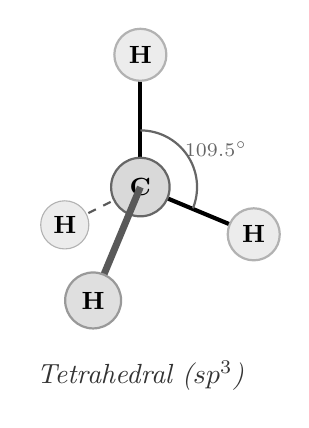
\begin{tikzpicture}[>=stealth, scale=1.2, font=\small]
  % Back Bond (Dashed)
  \draw[thick, dashed, gray!70!black] (0,0) -- (-0.8,-0.4);
  \node[circle, fill=gray!15, draw=gray!60, inner sep=2.5pt] at (-0.8,-0.4) {\textbf{H}};

  % Central Atom and Solid Bonds
  \draw[line width=1.5pt] (0,0) -- (0, 1.4);
  \draw[line width=1.5pt] (0,0) -- ( 1.2,-0.5);
  \node[circle, fill=gray!30, draw=gray!80!black, thick, inner sep=4pt] (C) at (0,0) {\textbf{C}};
  \node[circle, fill=gray!15, draw=gray!60, thick, inner sep=3pt] at (0, 1.4) {\textbf{H}};
  \node[circle, fill=gray!15, draw=gray!60, thick, inner sep=3pt] at ( 1.2,-0.5) {\textbf{H}};

  % Front Bond (Wedge)
  \draw[line width=2.5pt, gray!70!black] (0,0) -- (-0.5,-1.2);
  \node[circle, fill=gray!25, draw=gray!80, thick, inner sep=3.5pt] at (-0.5,-1.2) {\textbf{H}};

  % Angle arc
  \draw[thick, gray!80!black] (0, 0.6) arc[start angle=90, end angle=-22, radius=0.6cm];
  \node[font=\scriptsize\bfseries, gray!80!black] at (0.8, 0.4) {$109.5^\circ$};

  \node[font=\itshape, text=black!80] at (0,-2.0) {Tetrahedral ($sp^3$)};
\end{tikzpicture}
\end{center}

\medskip
\begin{center}
\renewcommand{\arraystretch}{1.4}
\begin{tabular}{lcccccc}
\toprule
\textbf{Molecule} & \textbf{BP} & \textbf{LP} & \textbf{Hybrid} & \textbf{Shape} & \textbf{Bond Angle} \\
\midrule
H$_2$O  & 2 & 2 & $sp^3$ & Bent            & $104.5^\circ$ \\
NH$_3$  & 3 & 1 & $sp^3$ & Trigonal Pyramidal & $107^\circ$ \\
BaCl$_2$& 2 & 0 & $sp$   & Linear          & $180^\circ$   \\
CH$_4$  & 4 & 0 & $sp^3$ & Tetrahedral     & $109.5^\circ$ \\
\bottomrule
\end{tabular}
\end{center}

\end{tcolorbox}
\item Discuss the basic features of the VSEPR model. Explain why the magnitude of repulsion decreases in this order: lone pair--lone pair $>$ lone pair--bond pair $>$ bond pair--bond pair. \mk{13}
\yr{CHEM 113 | 2011--12}

\begin{tcolorbox}[enhanced,breakable,ansbox,colback=cB!4,colframe=cB,boxrule=0.8pt,arc=5pt,title={\textbf{Answer}},fonttitle=\bfseries\color{white},colbacktitle=cB]

%---------------------------------------------------------
\textbf{Basic Features of VSEPR Model}
%---------------------------------------------------------

\begin{itemize}[itemsep=4pt]
  \item Electron pairs (both BP and LP) in the valence shell of the central atom
        \textbf{repel each other} and arrange to be as far apart as possible to
        minimize total repulsion energy.

  \item The \textbf{total number of electron pairs} (BP + LP) around the central
        atom determines the \textbf{electron pair geometry}.

  \item The \textbf{molecular shape} is determined only by the positions of the
        \textbf{bonding pairs}; lone pairs are invisible in the final shape but
        influence bond angles.

  \item \textbf{Lone pairs occupy more space} than bonding pairs since they are
        attracted to only one nucleus (not shared), creating a larger, more diffuse
        electron cloud.

  \item \textbf{Order of repulsion:}
        \begin{center}
          LP--LP $>$ LP--BP $>$ BP--BP
        \end{center}

  \item \textbf{Multiple bonds} (double, triple) repel more strongly than single
        bonds and are treated as a single ``super pair'' in VSEPR.

  \item \textbf{Bond angles} decrease as lone pairs replace bonding pairs around
        the central atom.
\end{itemize}

\begin{center}
\renewcommand{\arraystretch}{1.4}
\begin{tabular}{cccll}
\toprule
\textbf{BP} & \textbf{LP} & \textbf{Total} & \textbf{Electron Geometry} & \textbf{Molecular Shape}\\
\midrule
2 & 0 & 2 & Linear             & Linear\\
3 & 0 & 3 & Trigonal Planar    & Trigonal Planar\\
2 & 1 & 3 & Trigonal Planar    & Bent\\
4 & 0 & 4 & Tetrahedral        & Tetrahedral\\
3 & 1 & 4 & Tetrahedral        & Trigonal Pyramidal\\
2 & 2 & 4 & Tetrahedral        & Bent\\
5 & 0 & 5 & Trig.\ Bipyramidal & Trig.\ Bipyramidal\\
4 & 1 & 5 & Trig.\ Bipyramidal & See-Saw\\
3 & 2 & 5 & Trig.\ Bipyramidal & T-Shape\\
6 & 0 & 6 & Octahedral         & Octahedral\\
5 & 1 & 6 & Octahedral         & Square Pyramidal\\
4 & 2 & 6 & Octahedral         & Square Planar\\
\bottomrule
\end{tabular}
\end{center}

\medskip
%---------------------------------------------------------
\textbf{Why LP--LP $>$ LP--BP $>$ BP--BP repulsion}
%---------------------------------------------------------

\begin{itemize}[itemsep=5pt]

  \item \textbf{Lone pair--Lone pair (LP--LP) repulsion is greatest:}\\
        A lone pair is attracted to \textbf{only one nucleus}. It is not confined
        between two nuclei like a bonding pair, so it spreads out and occupies a
        \textbf{larger region of space}. When two such diffuse, large electron
        clouds are close to each other, their electrostatic repulsion is very
        strong. Hence LP--LP repulsion is maximum.

  \item \textbf{Lone pair--Bond pair (LP--BP) repulsion is intermediate:}\\
        A bonding pair is shared between two nuclei and is more
        \textbf{concentrated/localized} along the bond axis. When a lone pair
        (large cloud) interacts with a bonding pair (smaller, directed cloud),
        the repulsion is less than LP--LP but more than BP--BP since one partner
        is still a diffuse lone pair.

  \item \textbf{Bond pair--Bond pair (BP--BP) repulsion is least:}\\
        Both electron pairs are bonding pairs, each pulled toward \textbf{two
        nuclei} and therefore confined to a narrow region between the atoms.
        Two such localized, compact clouds repel each other the least.

\end{itemize}

\begin{center}
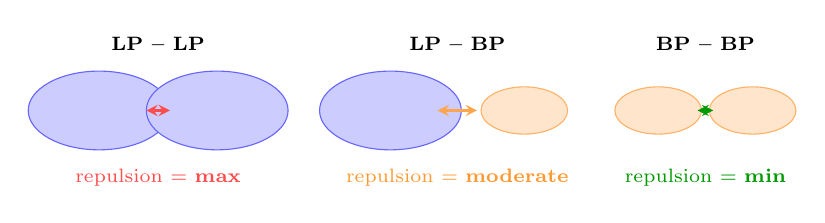
\begin{tikzpicture}[every node/.style={font=\small}, >=stealth]

  % LP-LP
  \draw[fill=blue!20,draw=blue!60] (-5.5,0) ellipse (0.9cm and 0.5cm);
  \draw[fill=blue!20,draw=blue!60] (-4.0,0) ellipse (0.9cm and 0.5cm);
  \node[font=\scriptsize] at (-4.75, 0.85) {\textbf{LP -- LP}};
  \node[font=\scriptsize,red!70] at (-4.75,-0.85) {repulsion = \textbf{max}};
  \draw[<->,red!70,thick] (-4.6,0)--(-4.9,0);

  % LP-BP
  \draw[fill=blue!20,draw=blue!60] (-1.8,0) ellipse (0.9cm and 0.5cm);
  \draw[fill=orange!20,draw=orange!60] (-0.1,0) ellipse (0.55cm and 0.3cm);
  \node[font=\scriptsize] at (-0.95, 0.85) {\textbf{LP -- BP}};
  \node[font=\scriptsize,orange!80] at (-0.95,-0.85) {repulsion = \textbf{moderate}};
  \draw[<->,orange!70,thick] (-0.7,0)--(-1.2,0);

  % BP-BP
  \draw[fill=orange!20,draw=orange!60] (1.6,0) ellipse (0.55cm and 0.3cm);
  \draw[fill=orange!20,draw=orange!60] (2.8,0) ellipse (0.55cm and 0.3cm);
  \node[font=\scriptsize] at (2.2, 0.85) {\textbf{BP -- BP}};
  \node[font=\scriptsize,green!60!black] at (2.2,-0.85) {repulsion = \textbf{min}};
  \draw[<->,green!60!black,thick] (2.1,0)--(2.3,0);

\end{tikzpicture}
\end{center}

\textbf{Effect on bond angles:} Each lone pair added to the central atom compresses
the remaining bond angles, e.g., CH$_4$ ($109.5^\circ$) $\rightarrow$ NH$_3$
($107^\circ$) $\rightarrow$ H$_2$O ($104.5^\circ$) as LP count increases from 0 to 2.

\end{tcolorbox}


\item Predict whether each of the following molecules has a dipole moment: BrCl; BF$_3$; CH$_2$Cl$_2$. \mk{6}
\yr{CHEM 113 | 2011--12}

\begin{tcolorbox}[enhanced,breakable,ansbox,colback=cB!4,colframe=cB,boxrule=0.8pt,arc=5pt,title={\textbf{Answer}},fonttitle=\bfseries\color{white},colbacktitle=cB]

%---------------------------------------------------------
\textbf{Dipole Moment Predictions}
%---------------------------------------------------------

A molecule has a net dipole moment if bond moments \textbf{do not cancel} due to
asymmetry in geometry or electronegativity.

\medskip
%---------------------------------------------------------
\textbf{(i) BrCl (Bromine monochloride)}
%---------------------------------------------------------

\begin{itemize}[itemsep=2pt, label=\textcolor{cB}{$\bullet$}]
  \item Diatomic molecule; Cl is more electronegative than Br.
  \item Bond moment points from Br $\rightarrow$ Cl (toward Cl).
  \item Only one bond $\Rightarrow$ \textbf{no cancellation possible}.
  \item \textbf{Dipole moment $\neq 0$ (polar molecule)}, $\mu > 0$
\end{itemize}

\begin{center}
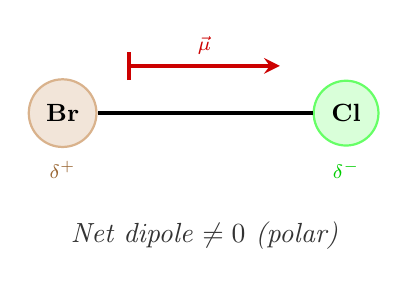
\begin{tikzpicture}[>=stealth, scale=1.2, font=\small]
  % Atoms and Bond
  \node[circle, fill=brown!20, draw=brown!60, thick, inner sep=4pt] (Br) at (-1.5,0) {\textbf{Br}};
  \node[circle, fill=green!15, draw=green!60, thick, inner sep=4pt] (Cl) at ( 1.5,0) {\textbf{Cl}};
  \draw[line width=1.5pt] (Br) -- (Cl);
  
  % Partial Charges
  \node[font=\scriptsize\bfseries, brown!80!black] at (-1.5, -0.6) {$\delta^+$};
  \node[font=\scriptsize\bfseries, green!80!black] at ( 1.5, -0.6) {$\delta^-$};
  
  % Dipole Arrow (Cross-tailed)
  \draw[->, line width=1.5pt, red!80!black] (-0.8, 0.5) -- (0.8, 0.5) node[midway, above, font=\scriptsize\bfseries] {$\vec{\mu}$};
  \draw[line width=1.5pt, red!80!black] (-0.8, 0.35) -- (-0.8, 0.65); % Cross part
  
  \node[font=\itshape, text=black!80] at (0,-1.3) {Net dipole $\neq 0$ (polar)};
\end{tikzpicture}
\end{center}

\medskip
%---------------------------------------------------------
\textbf{(ii) BF$_3$ (Boron trifluoride)}
%---------------------------------------------------------

\begin{itemize}[itemsep=2pt, label=\textcolor{cB}{$\bullet$}]
  \item B is central atom; BP $= 3$, LP $= 0$; \textbf{Hybridization:} $sp^2$
  \item \textbf{Shape: Trigonal Planar}, bond angle $= 120^\circ$
  \item F is more electronegative $\Rightarrow$ each B--F bond moment points toward F.
  \item Three bond moments at $120^\circ$ are \textbf{symmetrically arranged}
        $\Rightarrow$ they cancel completely.
  \item \textbf{Dipole moment $= 0$ (non-polar molecule)}
\end{itemize}

\begin{center}
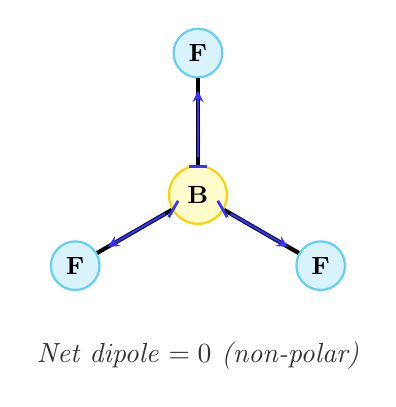
\begin{tikzpicture}[>=stealth, scale=1.2, font=\small]
  % Atoms
  \node[circle, fill=yellow!20, draw=yellow!70!orange, thick, inner sep=4pt] (B) at (0,0) {\textbf{B}};
  \node[circle, fill=cyan!15, draw=cyan!60, thick, inner sep=3pt] (F1) at (90:1.5) {\textbf{F}};
  \node[circle, fill=cyan!15, draw=cyan!60, thick, inner sep=3pt] (F2) at (210:1.5) {\textbf{F}};
  \node[circle, fill=cyan!15, draw=cyan!60, thick, inner sep=3pt] (F3) at (330:1.5) {\textbf{F}};
  
  % Bonds
  \draw[line width=1.5pt] (B) -- (F1);
  \draw[line width=1.5pt] (B) -- (F2);
  \draw[line width=1.5pt] (B) -- (F3);
  
  % Bond moments (using polar coordinates for perfect symmetry)
  \draw[->, thick, blue!80] (90:0.4) -- (90:1.1);
  \draw[line width=1pt, blue!80] (90:0.3) +(-0.1,0) -- +(0.1,0); % Cross
  
  \draw[->, thick, blue!80] (210:0.4) -- (210:1.1);
  \draw[line width=1pt, blue!80] (210:0.3) +(60:0.1) -- +(240:0.1); % Cross
  
  \draw[->, thick, blue!80] (330:0.4) -- (330:1.1);
  \draw[line width=1pt, blue!80] (330:0.3) +(120:0.1) -- +(300:0.1); % Cross
  
  \node[font=\itshape, text=black!80] at (0,-1.7) {Net dipole $= 0$ (non-polar)};
\end{tikzpicture}
\end{center}

\medskip
%---------------------------------------------------------
\textbf{(iii) CH$_2$Cl$_2$ (Dichloromethane)}
%---------------------------------------------------------

\begin{itemize}[itemsep=2pt, label=\textcolor{cB}{$\bullet$}]
  \item C is central atom; BP $= 4$, LP $= 0$; \textbf{Hybridization:} $sp^3$
  \item \textbf{Shape: Tetrahedral} (distorted), bond angle $\approx 109.5^\circ$
  \item Cl is more electronegative than H $\Rightarrow$ C--Cl bond moments point
        toward Cl; C--H bond moments point toward C (away from H).
  \item The molecule is \textbf{asymmetric}: 2 Cl on one side, 2 H on the other.
  \item Bond moments \textbf{do not cancel} $\Rightarrow$ net resultant exists.
  \item \textbf{Dipole moment $\neq 0$ (polar molecule)}
\end{itemize}

\begin{center}
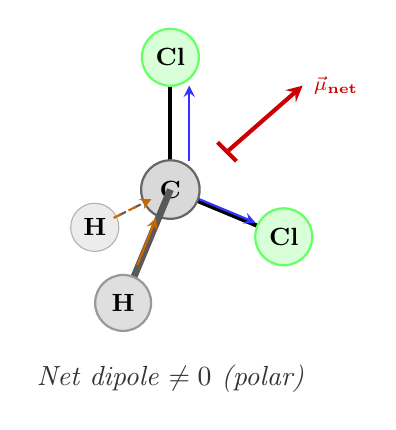
\begin{tikzpicture}[>=stealth, scale=1.2, font=\small]
  % Back Bond (H) - Dashed
  \draw[thick, dashed, gray!70!black] (0,0) -- (-0.8, -0.4);
  \node[circle, fill=gray!15, draw=gray!60, inner sep=2.5pt] at (-0.8, -0.4) {\textbf{H}};
  
  % Solid Bonds (in-plane)
  \draw[line width=1.5pt] (0,0) -- (0, 1.4);
  \draw[line width=1.5pt] (0,0) -- ( 1.2, -0.5);
  
  % Central Atom & Cl Atoms
  \node[circle, fill=gray!30, draw=gray!80!black, thick, inner sep=4pt] (C) at (0,0) {\textbf{C}};
  \node[circle, fill=green!15, draw=green!60, thick, inner sep=3pt] at (0, 1.4) {\textbf{Cl}};
  \node[circle, fill=green!15, draw=green!60, thick, inner sep=3pt] at ( 1.2, -0.5) {\textbf{Cl}};
  
  % Front Bond (H) - Wedge
  \draw[line width=2.5pt, gray!70!black] (0,0) -- (-0.5, -1.2);
  \node[circle, fill=gray!25, draw=gray!80, thick, inner sep=3.5pt] at (-0.5, -1.2) {\textbf{H}};
  
  % Bond Moments
  \draw[->, thick, blue!80] (0.2, 0.3) -- (0.2, 1.1); % C to Cl (Up)
  \draw[->, thick, blue!80] (0.3, -0.1) -- (0.9, -0.35); % C to Cl (Right)
  \draw[->, thick, orange!80!black] (-0.35, -0.8) -- (-0.15, -0.3); % H to C (Front)
  \draw[->, thick, orange!80!black, dashed] (-0.6, -0.3) -- (-0.2, -0.1); % H to C (Back)
  
  % Net Dipole Arrow (Cross-tailed)
  \draw[->, line width=1.5pt, red!80!black] (0.6, 0.4) -- (1.4, 1.1) node[right, font=\scriptsize\bfseries] {$\vec{\mu}_{\text{net}}$};
  \draw[line width=1.5pt, red!80!black] (0.5, 0.5) -- (0.7, 0.3); % Cross part
  
  \node[font=\itshape, text=black!80] at (0,-2.0) {Net dipole $\neq 0$ (polar)};
\end{tikzpicture}
\end{center}

\begin{center}
\renewcommand{\arraystretch}{1.4}
\begin{tabular}{llll}
\toprule
\textbf{Molecule} & \textbf{Shape} & \textbf{Bond moments cancel?} & \textbf{Dipole moment}\\
\midrule
BrCl        & Linear (diatomic)  & No  & $\neq 0$ (polar)\\
BF$_3$      & Trigonal Planar    & Yes & $= 0$ (non-polar)\\
CH$_2$Cl$_2$& Tetrahedral        & No  & $\neq 0$ (polar)\\
\bottomrule
\end{tabular}
\end{center}

\end{tcolorbox}

\item Discuss the basis of determining the molecular structure by Valence Shell Electron Pair Repulsion (VSEPR) theory. Determine structure of H$_2$O, BrF$_3$ and ICl$_4^-$ according to VSEPR theory. \mk{10}
\yr{CHEM 101 | 2009--10}
\begin{tcolorbox}[enhanced,breakable,ansbox,colback=cB!4,colframe=cB,boxrule=0.8pt,arc=5pt,title={\textbf{Answer}},fonttitle=\bfseries\color{white},colbacktitle=cB]

%---------------------------------------------------------
\textbf{Basis of VSEPR Theory}
%---------------------------------------------------------

The \textbf{Valence Shell Electron Pair Repulsion (VSEPR)} theory predicts molecular
geometry based on the following principles:

\begin{itemize}[itemsep=4pt, label=\textcolor{cB}{$\bullet$}]
  \item Electron pairs (both bonding and lone pairs) in the valence shell of the
        central atom \textbf{repel each other} and arrange themselves to be as
        far apart as possible to minimize repulsion.

  \item The \textbf{order of repulsion} between electron pairs is:\\
        \begin{center}
          LP--LP $>$ LP--BP $>$ BP--BP
        \end{center}

  \item Lone pairs occupy \textbf{more space} than bonding pairs (not shared between
        two nuclei), causing greater repulsion and \textbf{compressing bond angles}.

  \item The total number of electron pairs (BP + LP) around the central atom
        determines the \textbf{electron geometry}; the positions of bonding pairs
        alone determine the \textbf{molecular shape}.

  \item \textbf{Steps to determine structure:}
    \begin{enumerate}[label=\textcolor{cB}{(\roman*)}, itemsep=2pt]
      \item Count total valence electrons.
      \item Identify the central atom and form bonds with surrounding atoms.
      \item Distribute remaining electrons as lone pairs.
      \item Count BP and LP on central atom.
      \item Use the table below to predict geometry.
    \end{enumerate}
\end{itemize}

\begin{center}
\renewcommand{\arraystretch}{1.4}
\begin{tabular}{cccll}
\toprule
\textbf{BP} & \textbf{LP} & \textbf{Total} & \textbf{Electron Geometry} & \textbf{Molecular Shape}\\
\midrule
2 & 0 & 2 & Linear            & Linear\\
3 & 0 & 3 & Trigonal Planar   & Trigonal Planar\\
2 & 1 & 3 & Trigonal Planar   & Bent\\
4 & 0 & 4 & Tetrahedral       & Tetrahedral\\
3 & 1 & 4 & Tetrahedral       & Trigonal Pyramidal\\
2 & 2 & 4 & Tetrahedral       & Bent\\
5 & 0 & 5 & Trig.\ Bipyramidal & Trig.\ Bipyramidal\\
4 & 1 & 5 & Trig.\ Bipyramidal & See-Saw\\
3 & 2 & 5 & Trig.\ Bipyramidal & T-Shape\\
6 & 0 & 6 & Octahedral        & Octahedral\\
5 & 1 & 6 & Octahedral        & Square Pyramidal\\
4 & 2 & 6 & Octahedral        & Square Planar\\
\bottomrule
\end{tabular}
\end{center}

\medskip
%---------------------------------------------------------
\textbf{(i) H$_2$O (Water)}
%---------------------------------------------------------

\begin{itemize}[itemsep=2pt, label=\textcolor{cB}{$\bullet$}]
  \item \textbf{Valence electrons:} $6 + 2\times1 = 8$ electrons
  \item O is central atom; 2 O--H bonds formed; remaining $8-4=4$ electrons
        $\Rightarrow$ 2 LP on O
  \item BP $= 2$, LP $= 2$ $\Rightarrow$ Total $= 4$
  \item \textbf{Hybridization:} $sp^3$
  \item Electron geometry: Tetrahedral
  \item \textbf{Molecular shape: Bent (V-shaped)}
  \item Bond angle $\approx 104.5^\circ$ (compressed from $109.5^\circ$ by strong LP--LP repulsion)
\end{itemize}

\begin{center}
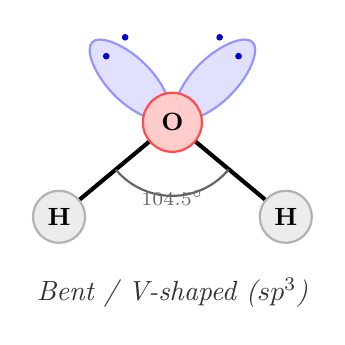
\begin{tikzpicture}[>=stealth, scale=1.2, font=\small]
  % LP Lobes
  \filldraw[rotate=135, fill=blue!15, draw=blue!50, thick, opacity=0.8] 
    (0,0) .. controls (0.4,0.4) and (1.2,0.2) .. (1.2,0) .. controls (1.2,-0.2) and (0.4,-0.4) .. (0,0);
  \filldraw[rotate=45, fill=blue!15, draw=blue!50, thick, opacity=0.8] 
    (0,0) .. controls (0.4,0.4) and (1.2,0.2) .. (1.2,0) .. controls (1.2,-0.2) and (0.4,-0.4) .. (0,0);
  \fill[blue!80!black] (-0.7, 0.7) circle (1pt); \fill[blue!80!black] (-0.5, 0.9) circle (1pt);
  \fill[blue!80!black] ( 0.7, 0.7) circle (1pt); \fill[blue!80!black] ( 0.5, 0.9) circle (1pt);

  % Bonds
  \draw[line width=1.5pt] (0,0) -- (-1.2,-1.0);
  \draw[line width=1.5pt] (0,0) -- ( 1.2,-1.0);

  % Atoms
  \node[circle, fill=red!20, draw=red!70, thick, inner sep=4pt] (O) at (0,0) {\textbf{O}};
  \node[circle, fill=gray!15, draw=gray!60, thick, inner sep=3pt] at (-1.2,-1.0) {\textbf{H}};
  \node[circle, fill=gray!15, draw=gray!60, thick, inner sep=3pt] at ( 1.2,-1.0) {\textbf{H}};

  % Angle arc
  \draw[thick, gray!80!black] (-0.6,-0.5) arc[start angle=220, end angle=320, radius=0.78cm];
  \node[font=\scriptsize\bfseries, gray!80!black] at (0,-0.8) {$104.5^\circ$};

  \node[font=\itshape, text=black!80] at (0,-1.8) {Bent / V-shaped ($sp^3$)};
\end{tikzpicture}
\end{center}

\medskip
%---------------------------------------------------------
\textbf{(ii) BrF$_3$ (Bromine Trifluoride)}
%---------------------------------------------------------

\begin{itemize}[itemsep=2pt, label=\textcolor{cB}{$\bullet$}]
  \item \textbf{Valence electrons:} $7 + 3\times7 = 28$ electrons
  \item Br is central atom; 3 Br--F bonds formed (6 electrons);
        remaining $28-6-18=4$ electrons $\Rightarrow$ 2 LP on Br
  \item BP $= 3$, LP $= 2$ $\Rightarrow$ Total $= 5$
  \item \textbf{Hybridization:} $sp^3d$
  \item Electron geometry: Trigonal Bipyramidal
  \item LPs occupy \textbf{equatorial} positions (minimize $90^\circ$ repulsions)
  \item \textbf{Molecular shape: T-shaped}
  \item Bond angles $< 90^\circ$ (compressed by LP--BP repulsions)
\end{itemize}

\begin{center}
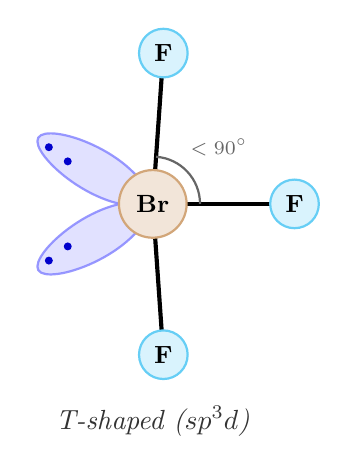
\begin{tikzpicture}[>=stealth, scale=1.2, font=\small]
  % Equatorial LP Lobes (Left side)
  \filldraw[rotate=150, fill=blue!15, draw=blue!50, thick, opacity=0.8] 
    (0,0) .. controls (0.4,0.4) and (1.4,0.2) .. (1.4,0) .. controls (1.4,-0.2) and (0.4,-0.4) .. (0,0);
  \fill[blue!80!black] (-0.9, 0.45) circle (1.2pt); \fill[blue!80!black] (-1.1, 0.6) circle (1.2pt);

  \filldraw[rotate=210, fill=blue!15, draw=blue!50, thick, opacity=0.8] 
    (0,0) .. controls (0.4,0.4) and (1.4,0.2) .. (1.4,0) .. controls (1.4,-0.2) and (0.4,-0.4) .. (0,0);
  \fill[blue!80!black] (-0.9, -0.45) circle (1.2pt); \fill[blue!80!black] (-1.1, -0.6) circle (1.2pt);

  % Bonds (Bent slightly to the right due to LP repulsion)
  \draw[line width=1.5pt] (0,0) -- (86:1.6);
  \draw[line width=1.5pt] (0,0) -- (-86:1.6);
  \draw[line width=1.5pt] (0,0) -- (0:1.5);

  % Atoms
  \node[circle, fill=brown!20, draw=brown!70, thick, inner sep=4pt] (Br) at (0,0) {\textbf{Br}};
  \node[circle, fill=cyan!15, draw=cyan!60, thick, inner sep=3pt] at (86:1.6) {\textbf{F}};
  \node[circle, fill=cyan!15, draw=cyan!60, thick, inner sep=3pt] at (-86:1.6) {\textbf{F}};
  \node[circle, fill=cyan!15, draw=cyan!60, thick, inner sep=3pt] at (0:1.5) {\textbf{F}};

  % Angle arc
  \draw[thick, gray!80!black] (0.5, 0) arc[start angle=0, end angle=86, radius=0.5cm];
  \node[font=\scriptsize\bfseries, gray!80!black] at (0.7, 0.6) {$<90^\circ$};

  \node[font=\itshape, text=black!80] at (0,-2.3) {T-shaped ($sp^3d$)};
\end{tikzpicture}
\end{center}

\medskip
%---------------------------------------------------------
\textbf{(iii) ICl$_4^-$ (Tetrachloroiodate ion)}
%---------------------------------------------------------

\begin{itemize}[itemsep=2pt, label=\textcolor{cB}{$\bullet$}]
  \item \textbf{Valence electrons:} $7 + 4\times7 + 1 = 36$ electrons
  \item I is central atom; 4 I--Cl bonds formed (8 electrons);
        remaining $36-8-24=4$ electrons $\Rightarrow$ 2 LP on I
  \item BP $= 4$, LP $= 2$ $\Rightarrow$ Total $= 6$
  \item \textbf{Hybridization:} $sp^3d^2$
  \item Electron geometry: Octahedral
  \item LPs occupy \textbf{opposite axial positions} (trans to each other $\Rightarrow$
        LP--LP repulsion minimized at $180^\circ$)
  \item \textbf{Molecular shape: Square Planar}
  \item Bond angle $= 90^\circ$
\end{itemize}

\begin{center}
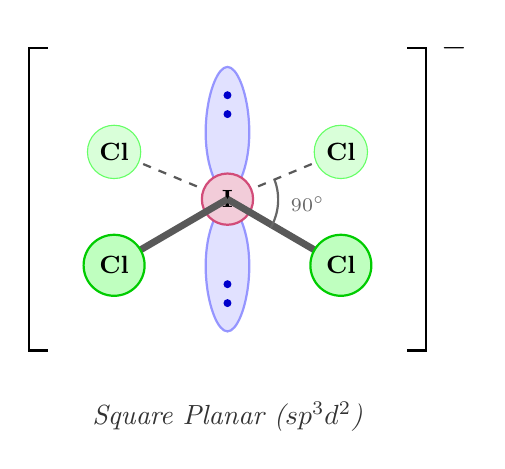
\begin{tikzpicture}[>=stealth, scale=1.2, font=\small]
  % Axial LP Lobes (Top & Bottom)
  \filldraw[rotate=90, fill=blue!15, draw=blue!50, thick, opacity=0.8] 
    (0,0) .. controls (0.4,0.4) and (1.4,0.2) .. (1.4,0) .. controls (1.4,-0.2) and (0.4,-0.4) .. (0,0);
  \fill[blue!80!black] (0, 0.9) circle (1.2pt); \fill[blue!80!black] (0, 1.1) circle (1.2pt);

  \filldraw[rotate=-90, fill=blue!15, draw=blue!50, thick, opacity=0.8] 
    (0,0) .. controls (0.4,0.4) and (1.4,0.2) .. (1.4,0) .. controls (1.4,-0.2) and (0.4,-0.4) .. (0,0);
  \fill[blue!80!black] (0, -0.9) circle (1.2pt); \fill[blue!80!black] (0, -1.1) circle (1.2pt);

  % Back Bonds (Dashed)
  \draw[thick, dashed, gray!70!black] (0,0) -- (-1.2, 0.5);
  \draw[thick, dashed, gray!70!black] (0,0) -- ( 1.2, 0.5);
  \node[circle, fill=green!15, draw=green!60, inner sep=2.5pt] at (-1.2, 0.5) {\textbf{Cl}};
  \node[circle, fill=green!15, draw=green!60, inner sep=2.5pt] at ( 1.2, 0.5) {\textbf{Cl}};

  % Central Atom
  \node[circle, fill=purple!20, draw=purple!70, thick, inner sep=4pt] (I) at (0,0) {\textbf{I}};

  % Front Bonds (Wedge)
  \draw[line width=2.5pt, gray!70!black] (0,0) -- (-1.2, -0.7);
  \draw[line width=2.5pt, gray!70!black] (0,0) -- ( 1.2, -0.7);
  \node[circle, fill=green!25, draw=green!80!black, thick, inner sep=3.5pt] at (-1.2, -0.7) {\textbf{Cl}};
  \node[circle, fill=green!25, draw=green!80!black, thick, inner sep=3.5pt] at ( 1.2, -0.7) {\textbf{Cl}};

  % Angle Arc
  \draw[thick, gray!80!black] (0.5, 0.2) arc[start angle=20, end angle=-30, radius=0.6cm];
  \node[font=\scriptsize\bfseries, gray!80!black] at (0.85, -0.05) {$90^\circ$};

  % Bracket and Charge
  \draw[line width=1pt] (-1.9, 1.6) -- (-2.1, 1.6) -- (-2.1, -1.6) -- (-1.9, -1.6);
  \draw[line width=1pt] ( 1.9, 1.6) -- ( 2.1, 1.6) -- ( 2.1, -1.6) -- ( 1.9, -1.6);
  \node[font=\large\bfseries] at (2.4, 1.6) {$-$};

  \node[font=\itshape, text=black!80] at (0,-2.3) {Square Planar ($sp^3d^2$)};
\end{tikzpicture}
\end{center}

\medskip
\begin{center}
\renewcommand{\arraystretch}{1.4}
\begin{tabular}{lccccl}
\toprule
\textbf{Species} & \textbf{BP} & \textbf{LP} & \textbf{Hybrid} & \textbf{Shape} & \textbf{Bond Angle}\\
\midrule
H$_2$O      & 2 & 2 & $sp^3$    & Bent          & $104.5^\circ$\\
BrF$_3$     & 3 & 2 & $sp^3d$   & T-shaped      & $<90^\circ$\\
ICl$_4^-$   & 4 & 2 & $sp^3d^2$ & Square Planar & $90^\circ$\\
\bottomrule
\end{tabular}
\end{center}

\end{tcolorbox}

\item Discuss hybridization and the valence shell electron pair repulsion model in determining the structure of molecules. Cite suitable examples. \mk{12}
\yr{CHEM 101 | 2008--09}
\begin{tcolorbox}[enhanced,breakable,ansbox,colback=cB!4,colframe=cB,boxrule=0.8pt,arc=5pt,title={\textbf{Answer}},fonttitle=\bfseries\color{white},colbacktitle=cB]

%---------------------------------------------------------
\textbf{Hybridization and VSEPR in Determining Molecular Structure}
%---------------------------------------------------------

\textbf{Hybridization (VBT):}

\begin{itemize}[itemsep=3pt, label=\textcolor{cB}{$\bullet$}]
  \item Hybridization is the \textbf{mixing of atomic orbitals} of similar energy
        on the same atom to produce a new set of equivalent hybrid orbitals.
  \item Number of hybrid orbitals $=$ number of orbitals mixed.
  \item Hybrid orbitals are directed in space to \textbf{minimize repulsion} and
        form stronger bonds by better overlap.
  \item Explains molecular geometry and bond angles.
\end{itemize}

\begin{center}
\renewcommand{\arraystretch}{1.3}
\begin{tabular}{llcll}
\toprule
\textbf{Hybrid} & \textbf{Orbitals} & \textbf{No.} & \textbf{Geometry} & \textbf{Example}\\
\midrule
$sp$      & $s+p$           & 2 & Linear             & BeCl$_2$\\
$sp^2$    & $s+p+p$         & 3 & Trigonal Planar    & BF$_3$\\
$sp^3$    & $s+p+p+p$       & 4 & Tetrahedral        & CH$_4$\\
$sp^3d$   & $s+p+p+p+d$     & 5 & Trig.\ Bipyramidal & PCl$_5$\\
$sp^3d^2$ & $s+p+p+p+d+d$   & 6 & Octahedral         & SF$_6$\\
\bottomrule
\end{tabular}
\end{center}

\medskip
\textbf{VSEPR Model:}

\begin{itemize}[itemsep=3pt, label=\textcolor{cB}{$\bullet$}]
  \item Electron pairs (BP + LP) repel each other and arrange to
        \textbf{minimize repulsion}.
  \item Repulsion order: LP--LP $>$ LP--BP $>$ BP--BP.
  \item Molecular shape depends on BP arrangement; LP invisible but compress angles.
\end{itemize}

\medskip
\textbf{Illustrative Examples ($sp^3$ Family Comparison):}

\medskip

\begin{itemize}[itemsep=3pt, label=\textcolor{cB}{$\bullet$}]
  \item \textbf{CH$_4$ (Tetrahedral):} BP $= 4$, LP $= 0$; pure $sp^3$, no LP compression ($109.5^\circ$).
  \item \textbf{NH$_3$ (Trigonal Pyramidal):} BP $= 3$, LP $= 1$; LP--BP repulsion compresses angle to $107^\circ$.
  \item \textbf{H$_2$O (Bent):} BP $= 2$, LP $= 2$; strong LP--LP repulsion compresses angle to $104.5^\circ$.
\end{itemize}

\vspace{0.3cm}

\begin{center}
\makebox[\textwidth][c]{
% --- CH4 ---
\begin{tikzpicture}[>=stealth, scale=1.1, font=\small]
  \node[font=\large\bfseries, text=black!80] at (0, 2.2) {CH$_4$};
  
  % Back Bond (dashed)
  \draw[thick, dashed, gray!70!black] (0,0) -- (0.8, -0.6);
  \node[circle, fill=gray!15, draw=gray!60, inner sep=2.5pt] at (0.8, -0.6) {\textbf{H}};
  
  % In-plane bonds
  \draw[line width=1.5pt] (0,0) -- (0, 1.3);
  \draw[line width=1.5pt] (0,0) -- (-1.1, -0.5);
  
  % Central Atom
  \node[circle, fill=gray!30, draw=gray!80!black, thick, inner sep=4pt] (C) at (0,0) {\textbf{C}};
  \node[circle, fill=gray!15, draw=gray!60, thick, inner sep=3pt] at (0, 1.3) {\textbf{H}};
  \node[circle, fill=gray!15, draw=gray!60, thick, inner sep=3pt] at (-1.1, -0.5) {\textbf{H}};
  
  % Front Bond (Wedge)
  \draw[line width=2.5pt, gray!70!black] (0,0) -- (0.5, -1.2);
  \node[circle, fill=gray!25, draw=gray!80, thick, inner sep=3.5pt] at (0.5, -1.2) {\textbf{H}};
  
  % Label
  \node[font=\scriptsize\bfseries, gray!80!black] at (0,-1.9) {$109.5^\circ$};
  \node[font=\scriptsize, gray!80!black] at (0,-2.3) {Tetrahedral};
\end{tikzpicture}
\hfill
% --- NH3 ---
\begin{tikzpicture}[>=stealth, scale=1.1, font=\small]
  \node[font=\large\bfseries, text=black!80] at (0, 2.2) {NH$_3$};
  
  % LP Lobe (Top)
  \filldraw[rotate=90, fill=blue!15, draw=blue!50, thick, opacity=0.8] 
    (0,0) .. controls (0.4,0.4) and (1.3,0.2) .. (1.3,0) .. controls (1.3,-0.2) and (0.4,-0.4) .. (0,0);
  \fill[blue!80!black] (0, 0.7) circle (1.2pt); \fill[blue!80!black] (0, 0.9) circle (1.2pt);
  
  % Back Bond (dashed)
  \draw[thick, dashed, gray!70!black] (0,0) -- (0.8, -0.6);
  \node[circle, fill=gray!15, draw=gray!60, inner sep=2.5pt] at (0.8, -0.6) {\textbf{H}};
  
  % In-plane bond
  \draw[line width=1.5pt] (0,0) -- (-1.1, -0.5);
  
  % Central Atom
  \node[circle, fill=blue!20, draw=blue!70, thick, inner sep=4pt] (N) at (0,0) {\textbf{N}};
  \node[circle, fill=gray!15, draw=gray!60, thick, inner sep=3pt] at (-1.1, -0.5) {\textbf{H}};
  
  % Front Bond (Wedge)
  \draw[line width=2.5pt, gray!70!black] (0,0) -- (0.5, -1.2);
  \node[circle, fill=gray!25, draw=gray!80, thick, inner sep=3.5pt] at (0.5, -1.2) {\textbf{H}};
  
  % Label
  \node[font=\scriptsize\bfseries, gray!80!black] at (0,-1.9) {$107^\circ$};
  \node[font=\scriptsize, gray!80!black] at (0,-2.3) {Trigonal Pyramidal};
\end{tikzpicture}
\hfill
% --- H2O ---
\begin{tikzpicture}[>=stealth, scale=1.1, font=\small]
  \node[font=\large\bfseries, text=black!80] at (0, 2.2) {H$_2$O};
  
  % LP Lobes (Top Left & Top Right)
  \filldraw[rotate=135, fill=blue!15, draw=blue!50, thick, opacity=0.8] 
    (0,0) .. controls (0.4,0.4) and (1.2,0.2) .. (1.2,0) .. controls (1.2,-0.2) and (0.4,-0.4) .. (0,0);
  \filldraw[rotate=45, fill=blue!15, draw=blue!50, thick, opacity=0.8] 
    (0,0) .. controls (0.4,0.4) and (1.2,0.2) .. (1.2,0) .. controls (1.2,-0.2) and (0.4,-0.4) .. (0,0);
  \fill[blue!80!black] (-0.7, 0.7) circle (1.2pt); \fill[blue!80!black] (-0.5, 0.9) circle (1.2pt);
  \fill[blue!80!black] ( 0.7, 0.7) circle (1.2pt); \fill[blue!80!black] ( 0.5, 0.9) circle (1.2pt);

  % Bonds
  \draw[line width=1.5pt] (0,0) -- (-1.0,-0.9);
  \draw[line width=1.5pt] (0,0) -- ( 1.0,-0.9);

  % Central Atom & Hydrogens
  \node[circle, fill=red!20, draw=red!70, thick, inner sep=4pt] (O) at (0,0) {\textbf{O}};
  \node[circle, fill=gray!15, draw=gray!60, thick, inner sep=3pt] at (-1.0,-0.9) {\textbf{H}};
  \node[circle, fill=gray!15, draw=gray!60, thick, inner sep=3pt] at ( 1.0,-0.9) {\textbf{H}};
  
  % Label
  \node[font=\scriptsize\bfseries, gray!80!black] at (0,-1.9) {$104.5^\circ$};
  \node[font=\scriptsize, gray!80!black] at (0,-2.3) {Bent / V-shaped};
\end{tikzpicture}
}
\end{center}

\vspace{0.2cm}
\textbf{Conclusion:} Both hybridization and VSEPR complement each other ---
hybridization explains the \textit{type} of bonds formed, while VSEPR explains the
\textit{spatial arrangement} and bond angles.

\end{tcolorbox}

%%══════════════════════════════════════════════════════════════════════
%% S3 — Chemical Bonding
%%══════════════════════════════════════════════════════════════════════
\item What should be the possible geometrical structure of PCl$_5$ molecule? Justify on the basis of hybridization and VSEPR model. \mk{8}
\yr{CHEM 101 | 2006--07}

\begin{tcolorbox}[enhanced,breakable,ansbox,colback=cB!4,colframe=cB,boxrule=0.8pt,arc=5pt,title={\textbf{Answer}},fonttitle=\bfseries\color{white},colbacktitle=cB]

%---------------------------------------------------------
\textbf{Geometrical Structure of PCl$_5$}
%---------------------------------------------------------

%---------------------------------------------------------
\textbf{Part 1: Hybridization Approach}
%---------------------------------------------------------

\begin{itemize}[itemsep=3pt]
  \item \textbf{Valence electrons of P:} $1s^2\,2s^2\,2p^6\,3s^2\,3p^3$ ---
        ground state has 3 unpaired electrons, but P can expand its octet
        using empty $3d$ orbitals.

  \item \textbf{Excited state of P:} One electron from $3s$ is promoted to
        empty $3d$ orbital, giving 5 unpaired electrons available for bonding:
\end{itemize}

\begin{center}
\begin{tikzpicture}[every node/.style={font=\small}]
  % Ground state
  \node[anchor=east] at (-0.2, 1.5) {\textbf{Ground state (P):}};
  % 3s box
  \draw (0,1.2) rectangle (0.7,1.8);
  \node at (0.35,1.5) {$\uparrow\downarrow$};
  \node[font=\scriptsize] at (0.35,1.0) {$3s$};
  % 3p boxes
  \foreach \x/\a in {1.0/$\uparrow$, 1.8/$\uparrow$, 2.6/$\uparrow$}{
    \draw (\x,1.2) rectangle (\x+0.7,1.8);
    \node at (\x+0.35,1.5) {\a};
  }
  \node[font=\scriptsize] at (1.85,1.0) {$3p$};
  % 3d boxes
  \foreach \x in {3.6,4.4,5.2,6.0,6.8}{
    \draw (\x,1.2) rectangle (\x+0.7,1.8);
  }
  \node[font=\scriptsize] at (5.2,1.0) {$3d$ (empty)};

  % Excited state
  \node[anchor=east] at (-0.2, 0.0) {\textbf{Excited state (P):}};
  % 3s box
  \draw (0,-0.3) rectangle (0.7,0.3);
  \node at (0.35,0.0) {$\uparrow$};
  \node[font=\scriptsize] at (0.35,-0.5) {$3s$};
  % 3p boxes
  \foreach \x/\a in {1.0/$\uparrow$, 1.8/$\uparrow$, 2.6/$\uparrow$}{
    \draw (\x,-0.3) rectangle (\x+0.7,0.3);
    \node at (\x+0.35,0.0) {\a};
  }
  \node[font=\scriptsize] at (1.85,-0.5) {$3p$};
  % 3d boxes (one filled)
  \draw (3.6,-0.3) rectangle (4.3, 0.3);
  \node at (3.95, 0.0) {$\uparrow$};
  \foreach \x in {4.4,5.2,6.0,6.8}{
    \draw (\x,-0.3) rectangle (\x+0.7,0.3);
  }
  \node[font=\scriptsize] at (5.2,-0.5) {$3d$};
\end{tikzpicture}
\end{center}

\begin{itemize}[itemsep=3pt]
  \item The 5 half-filled orbitals ($3s + 3p_x + 3p_y + 3p_z + 3d$) undergo
        \textbf{$sp^3d$ hybridization} to form 5 equivalent hybrid orbitals.
  \item Each hybrid orbital overlaps with a half-filled $3p$ orbital of Cl
        to form \textbf{5 P--Cl $\sigma$ bonds}.
  \item BP $= 5$, LP $= 0$ $\Rightarrow$ \textbf{Trigonal Bipyramidal geometry}.
\end{itemize}

\medskip
%---------------------------------------------------------
\textbf{Part 2: VSEPR Approach}
%---------------------------------------------------------

\begin{itemize}[itemsep=3pt]
  \item \textbf{Valence electrons:} $5 + 5\times7 = 40$ electrons
  \item P forms 5 bonds with Cl; no lone pairs remain on P.
  \item BP $= 5$, LP $= 0$ $\Rightarrow$ Total electron pairs $= 5$
  \item To minimize repulsion, 5 electron pairs arrange in a
        \textbf{Trigonal Bipyramidal} geometry.
  \item This gives \textbf{two distinct types} of P--Cl bonds:
\end{itemize}

\begin{center}
\renewcommand{\arraystretch}{1.4}
\begin{tabular}{lcc}
\toprule
\textbf{Position} & \textbf{No.\ of bonds} & \textbf{Bond angle}\\
\midrule
Equatorial (in plane) & 3 & $120^\circ$ with each other\\
Axial (above \& below) & 2 & $90^\circ$ with equatorial, $180^\circ$ with each other\\
\bottomrule
\end{tabular}
\end{center}

\begin{itemize}[itemsep=3pt]
  \item Equatorial P--Cl bonds are slightly \textbf{longer} than axial bonds
        (more BP--BP repulsion from equatorial side).
  \item The molecule is \textbf{non-polar} as all bond moments cancel by symmetry.
\end{itemize}

\medskip
%---------------------------------------------------------
\textbf{3D Structure of PCl$_5$}
%---------------------------------------------------------

\begin{center}
\begin{tikzpicture}[>=stealth, scale=1.2, font=\small]
  
  % Equatorial plane (dashed ellipse for 3D perspective)
  \draw[dashed, gray!60, line width=0.8pt] (0,0) ellipse (2cm and 0.55cm);

  % ==========================================
  % 1. BACK ELEMENTS (Drawn first to be behind)
  % ==========================================
  
  % Eq Back Bond & Cl (Dash)
  \draw[thick, dashed, gray!70!black] (0,0) -- (-1.0, 0.48);
  \node[circle, fill=green!15, draw=green!60, inner sep=2.5pt] at (-1.0, 0.48) {\textbf{Cl}};

  % ==========================================
  % 2. MIDDLE ELEMENTS (In-plane)
  % ==========================================
  
  % Axial Bonds
  \draw[line width=1.5pt] (0,0) -- (0, 2);
  \draw[line width=1.5pt] (0,0) -- (0, -2);
  % Eq Right Bond
  \draw[line width=1.5pt] (0,0) -- (2, 0);

  % Central P Atom
  \node[circle, fill=orange!20, draw=orange!80!black, thick, inner sep=4pt] (P) at (0,0) {\textbf{P}};

  % Axial Cl Atoms
  \node[circle, fill=green!15, draw=green!60, thick, inner sep=3pt] (ClAxTop) at (0, 2) {\textbf{Cl}};
  \node[circle, fill=green!15, draw=green!60, thick, inner sep=3pt] (ClAxBot) at (0, -2) {\textbf{Cl}};
  
  % Eq Right Cl Atom
  \node[circle, fill=green!15, draw=green!60, thick, inner sep=3pt] (ClEqRight) at (2, 0) {\textbf{Cl}};

  % ==========================================
  % 3. FRONT ELEMENTS (Drawn last to overlap)
  % ==========================================
  
  % Eq Front Bond & Cl (Wedge)
  \draw[line width=2.5pt, gray!70!black] (0,0) -- (-1.0, -0.48);
  \node[circle, fill=green!25, draw=green!80!black, thick, inner sep=3.5pt] (ClEqFront) at (-1.0, -0.48) {\textbf{Cl}};

  % ==========================================
  % 4. ANGLES & LABELS
  % ==========================================

  % 90 degree angle (Axial to Equatorial)
  \draw[thick, blue!80!black] (0.35, 0) arc[start angle=0, end angle=90, radius=0.35cm];
  \node[font=\scriptsize\bfseries, blue!80!black] at (0.6, 0.45) {$90^\circ$};

  % 120 degree angle (Equatorial to Equatorial)
  % Using elliptical arc to match 3D perspective
  \draw[thick, red!80!black] (1.2, 0) arc[start angle=0, end angle=-120, x radius=1.2cm, y radius=0.33cm];
  \node[font=\scriptsize\bfseries, red!80!black] at (0.7, -0.45) {$120^\circ$};

  % 180 degree angle (Axial to Axial)
  \draw[<->, thick, gray!80!black] (-0.5, 1.8) -- (-0.5, -1.8) node[midway, left, font=\scriptsize\bfseries] {$180^\circ$};

  % Pointers for axial/equatorial labels
  \draw[->, thick, gray!80!black] (ClAxTop) -- ++(1.0, 0.2) node[right, font=\scriptsize\itshape, text=black!80] {axial};
  \draw[->, thick, gray!80!black] (ClEqRight) -- ++(0.5, 0.5) node[right, font=\scriptsize\itshape, text=black!80] {equatorial};

  % Caption
  \node[font=\itshape, text=black!80] at (0, -2.8) {Trigonal Bipyramidal ($sp^3d$), BP $= 5$, LP $= 0$};

\end{tikzpicture}
\end{center}

\medskip
%---------------------------------------------------------
\textbf{Summary}
%---------------------------------------------------------

\begin{center}
\renewcommand{\arraystretch}{1.4}
\begin{tabular}{ll}
\toprule
\textbf{Property}            & \textbf{Value}\\
\midrule
Central atom                 & P\\
Hybridization                & $sp^3d$\\
BP / LP                      & 5 / 0\\
Electron geometry            & Trigonal Bipyramidal\\
Molecular shape              & Trigonal Bipyramidal\\
Equatorial bond angle        & $120^\circ$\\
Axial--equatorial bond angle & $90^\circ$\\
Axial--axial bond angle      & $180^\circ$\\
Dipole moment                & $0$ (non-polar)\\
\bottomrule
\end{tabular}
\end{center}

\end{tcolorbox}

\end{enumerate}
\newpage


\secdivider{Section S3}{Chemical Bonding}{cC}{cC}
\markboth{S3 --- Chemical Bonding}{}
\label{sec:S3}
\section{S3 --- Chemical Bonding}

\begin{enumerate}
\item Can you explain the existence of the transient ions like H$_2^+$? How? \mk{5}
\yr{CHEM 113 | 2023--24}

\begin{tcolorbox}[enhanced,breakable,ansbox,colback=cC!4,colframe=cC,boxrule=0.8pt,arc=5pt,title={\textbf{Answer}},fonttitle=\bfseries\color{white},colbacktitle=cC]
\textbf{Existence of Transient Ion H$_2^+$} \hfill \mk{5}

\medskip
\begin{center}
\textcolor{cC}{\rule{0.85\textwidth}{0.5pt}}
\end{center}

\medskip
\textbf{(i) What is H$_2^+$?}

H$_2^+$ is a \textbf{one-electron species} formed by removing one
electron from H$_2$. It consists of two protons held together by
a single electron. It is called \emph{transient} because it exists
only briefly under special conditions (e.g.\ electric discharge,
cosmic rays, or mass spectrometry).

\medskip
\textbf{(ii) MO Explanation of its Existence:}

Using LCAO, the two $1s$ atomic orbitals combine to give:
\[
  \Psi_b = \phi_{1s}^A + \phi_{1s}^B \quad (\sigma_{1s},
  \text{ bonding MO})
\]
\[
  \Psi^* = \phi_{1s}^A - \phi_{1s}^B \quad (\sigma^*_{1s},
  \text{ antibonding MO})
\]
H$_2^+$ has only \textbf{one electron}, which occupies the
bonding MO $\sigma_{1s}$:
\[
  \text{Configuration: } (\sigma_{1s})^1
\]
\[
  \text{Bond Order} = \tfrac{1}{2}(1 - 0) = \tfrac{1}{2}
\]

\begin{center}
  \begin{tikzpicture}[scale=1]

\def\sbaseline{0em};
\def\ssplit{8em};
\def\mwidth{3em};
\def\hsep{2em};

\tikzstyle{split} = [densely dashed,draw=gray]
\tikzstyle{orbital} = [rectangle, rounded corners, fill=white, draw=black, minimum width=3.5ex, minimum height=3.5ex]
\tikzstyle{label}    = [rectangle, minimum width=3.5ex, node distance=3.5ex]

% 1s splitting lines
\draw        (\mwidth/-2-\hsep*2,\sbaseline)             -- (\mwidth/-2-\hsep  ,\sbaseline);
\draw[split] (\mwidth/-2-\hsep  ,\sbaseline)             -- (\mwidth/-2        ,\sbaseline+\ssplit/2);
\draw        (\mwidth/-2        ,\sbaseline+\ssplit/2)   -- (\mwidth/2         ,\sbaseline+\ssplit/2);
\draw[split] (\mwidth/2         ,\sbaseline+\ssplit/2)   -- (\mwidth/2+\hsep   ,\sbaseline);
\draw        (\mwidth/2+\hsep   ,\sbaseline)             -- (\mwidth/+2+\hsep*2,\sbaseline);
\draw[split] (\mwidth/-2-\hsep  ,\sbaseline)             -- (\mwidth/-2        ,\sbaseline+\ssplit/-2);
\draw        (\mwidth/-2        ,\sbaseline+\ssplit/-2) -- (\mwidth/2         ,\sbaseline+\ssplit/-2);
\draw[split] (\mwidth/2         ,\sbaseline+\ssplit/-2) -- (\mwidth/2+\hsep   ,\sbaseline);

% Left Atom: H (1s^1)
\draw[] (-\mwidth-\hsep,0em) node[orbital] (l1s) {\moup};
\node[label, below of=l1s] (l1sl) {$1s$};

% Right Atom: H+ (1s^0)
\draw[] (\mwidth+\hsep,0em) node[orbital] (r1s) {};
\node[label, below of=r1s] (r1sl) {$1s$};

% Sigma Bonding (1 electron)
\draw[] (0em,\ssplit/-2) node[orbital] (sb) {\moup};
\node[label, below of=sb]  (sbl) {$\sigma_{1s}$};
\node[label, left of=sb, node distance = 9ex] {\tiny{\color{gray}{$\Psi_{a}+\Psi_{b}$}}};

% Sigma Antibonding (Empty)
\draw[] (0em,\ssplit/2) node[orbital] (sa) {};
\node[label, below of=sa] (sal) {$\sigma^{*}_{1s}$};
\node[label, left of=sa, node distance = 9ex] {\tiny{\color{gray}{$\Psi_{a}-\Psi_{b}$}}};

% Orbital labels (Atoms/Molecule)
\node[label, below of=l1sl, node distance=6em]   (a)    {\smash[b]{\ce{H}}};
\node[label, right of=a   , node distance=\mwidth*2]   (ab)   {\smash[b]{\ce{H$_2^+$}}};
\node[label, right of=a   , node distance=\mwidth*2+\hsep*2]  (b)    {\smash[b]{\ce{H$^+$}}};

% Title/Description
\node[label, below of=ab  , node distance=3em]   (desc) {Dihydrogen Cation (Bond order $= 0.5$)};

\end{tikzpicture}
\end{center}

\medskip
\textbf{(iii) Why it Can Exist:}
\begin{itemize}[leftmargin=1.5em, itemsep=3pt]
  \item Bond order $= \frac{1}{2} > 0$ --- a net bonding
        interaction exists.
  \item The single electron in $\sigma_{1s}$ creates
        \textbf{constructive interference} between the two
        nuclei, providing enough electron density to partially
        overcome nuclear repulsion.
  \item The system has a potential energy \textbf{minimum} at
        $r_0 = 1.06$ \AA\ --- confirming it is a bound state.
  \item Experimentally, H$_2^+$ has been detected in
        \textbf{mass spectrometers} and exists in
        \textbf{interstellar space}.
\end{itemize}

\medskip
\textbf{(iv) Why it is Transient:}
\begin{itemize}[leftmargin=1.5em, itemsep=2pt]
  \item Bond order of only $\frac{1}{2}$ means the bond is
        very \textbf{weak} (bond energy $= 255$ kJ/mol vs
        $436$ kJ/mol for H$_2$).
  \item Easily destroyed by collision with other molecules or
        by further ionization.
  \item Cannot be isolated under normal conditions.
\end{itemize}

\medskip
\begin{center}
\textcolor{cC}{\rule{0.85\textwidth}{0.5pt}}
\end{center}

\medskip
\textbf{Conclusion:} H$_2^+$ exists because MO theory predicts a
bond order of $\frac{1}{2}$ --- sufficient for a weak but real
bond. It is transient because this half-bond is too weak to survive
normal chemical conditions, yet strong enough to be detected
spectroscopically and in mass spectrometry.
\end{tcolorbox}

\item From the three possible ways to connect carbon, nitrogen, and oxygen to form a monoanion: CNO$^-$, CON$^-$ and OCN$^-$, one is the cyanate ion, a common and stable species; one is the fulminate ion, salts of which are used as explosive detonators; and one is so unstable that it has never been isolated. Use the concept of formal charge to determine which isomer is cyanate, which is the fulminate, and which is the least stable one. \mk{10}
\yr{CHEM 113 | 2023--24; 2020--21}

\begin{tcolorbox}[enhanced,breakable,ansbox,colback=cC!4,colframe=cC,boxrule=0.8pt,arc=5pt,title={\textbf{Answer}},fonttitle=\bfseries\color{white},colbacktitle=cC]
\textbf{Identifying CNO$^-$, CON$^-$, and OCN$^-$ Using Formal Charge}
\hfill \mk{10}

\medskip
\begin{center}
\textcolor{cC}{\rule{0.85\textwidth}{0.5pt}}
\end{center}

%% ── Background ────────────────────────────────────────────────────────
\medskip
\textbf{Background: Formal Charge Formula} \hfill \mk{1}

\medskip
The formal charge on an atom is calculated as:
\[
  \text{Formal Charge} = (\text{valence electrons})
  - (\text{lone pair electrons})
  - \tfrac{1}{2}(\text{bonding electrons})
\]
Valence electrons: C $= 4$, N $= 5$, O $= 6$.
Total valence electrons in the monoanion $= 4 + 5 + 6 + 1 = 16$.

\begin{center}
\textcolor{cC}{\rule{0.75\textwidth}{0.4pt}}
\end{center}

%% ── Isomer 1: OCN- ────────────────────────────────────────────────────
\medskip
\textbf{Isomer 1: OCN$^-$ (Cyanate Ion)} \hfill \mk{3}

\medskip
The dominant Lewis structure of OCN$^-$ is:
\[
  \underset{}{[\,\ddot{\text{O}} = \text{C} = \text{N}\,]}^{-}
  \quad\longleftrightarrow\quad
  [\,{:}\ddot{\text{O}} - \text{C} \equiv \text{N}\,{:}\,]^{-}
\]
Calculating formal charges for the structure
$\text{O}=\text{C}=\text{N}^-$:

\begin{center}
\begin{tabular}{p{0.12\textwidth} p{0.22\textwidth}
                p{0.22\textwidth} p{0.22\textwidth}}
\toprule
\textbf{Atom} & \textbf{Valence e$^-$} &
\textbf{LP + $\frac{1}{2}$BP} & \textbf{Formal Charge} \tabularnewline
\midrule
O & 6 & $4 + \frac{1}{2}(4) = 6$ & $6 - 6 = 0$ \tabularnewline[3pt]
C & 4 & $0 + \frac{1}{2}(8) = 4$ & $4 - 4 = 0$ \tabularnewline[3pt]
N & 5 & $4 + \frac{1}{2}(4) = 6$ & $5 - 6 = -1$ \tabularnewline
\bottomrule
\end{tabular}
\end{center}

\medskip
Formal charges: O $= 0$, C $= 0$, N $= -1$.
The negative charge resides on \textbf{nitrogen}, the most
electronegative atom after oxygen --- a chemically reasonable
distribution. The overall formal charges are small and the negative
charge is on a suitably electronegative atom.
\[
  \therefore\; \textbf{OCN}^- \text{ is the \textbf{cyanate ion} ---
  common and stable.}
\]

\begin{center}
\textcolor{cC}{\rule{0.75\textwidth}{0.4pt}}
\end{center}

%% ── Isomer 2: CNO- ────────────────────────────────────────────────────
\medskip
\textbf{Isomer 2: CNO$^-$ (Fulminate Ion)} \hfill \mk{3}

\medskip
The Lewis structure of CNO$^-$ places carbon at the terminal end:
\[
  [\,{:}\text{C} \equiv \text{N} - \ddot{\text{O}}{:}\,]^{-}
\]
Calculating formal charges for $\text{C}\equiv\text{N}{-}\text{O}$:

\begin{center}
\begin{tabular}{p{0.12\textwidth} p{0.22\textwidth}
                p{0.22\textwidth} p{0.22\textwidth}}
\toprule
\textbf{Atom} & \textbf{Valence e$^-$} &
\textbf{LP + $\frac{1}{2}$BP} & \textbf{Formal Charge} \tabularnewline
\midrule
C & 4 & $0 + \frac{1}{2}(6) = 3$ & $4 - 3 = +1$ \tabularnewline[3pt]
N & 5 & $0 + \frac{1}{2}(8) = 4$ & $5 - 4 = +1$ \tabularnewline[3pt]
O & 6 & $6 + \frac{1}{2}(2) = 7$ & $6 - 7 = -1$ \tabularnewline
\bottomrule
\end{tabular}
\end{center}

\medskip
Formal charges: C $= -1$, N $= +1$, O $= -1$.
Large formal charges of opposite signs create a highly
\emph{polar, strained} structure with significant internal
electrostatic tension. This stored energy is released explosively
upon detonation.
\[
  \therefore\; \textbf{CNO}^- \text{ is the \textbf{fulminate ion}
  --- explosive, used in detonators.}
\]

\begin{center}
\textcolor{cC}{\rule{0.75\textwidth}{0.4pt}}
\end{center}

%% ── Isomer 3: CON- ────────────────────────────────────────────────────
\medskip
\textbf{Isomer 3: CON$^-$ (Unstable, Never Isolated)} \hfill \mk{2}

\medskip
The Lewis structure of CON$^-$ places oxygen in the middle:
\[
  [\,{:}\text{C} = \text{O} = \text{N}{:}\,]^{-}
\]
Calculating formal charges for $\text{C}{=}\text{O}{=}\text{N}$:

\begin{center}
\begin{tabular}{p{0.12\textwidth} p{0.22\textwidth}
                p{0.22\textwidth} p{0.22\textwidth}}
\toprule
\textbf{Atom} & \textbf{Valence e$^-$} &
\textbf{LP + $\frac{1}{2}$BP} & \textbf{Formal Charge} \tabularnewline
\midrule
C & 4 & $2 + \frac{1}{2}(4) = 4$ & $4 - 4 = 0$ \tabularnewline[3pt]
O & 6 & $0 + \frac{1}{2}(8) = 4$ & $6 - 4 = +2$ \tabularnewline[3pt]
N & 5 & $4 + \frac{1}{2}(4) = 6$ & $5 - 6 = -1$ \tabularnewline
\bottomrule
\end{tabular}
\end{center}

\medskip
Formal charges: C $= 0$, O $= +2$, N $= -1$.
A formal charge of $+2$ on oxygen --- the most electronegative
element --- is extremely unfavorable. Placing positive charge on
the most electronegative atom violates chemical intuition and
creates a highly unstable electronic configuration. No resonance
structure can relieve this charge distribution.
\[
  \therefore\; \textbf{CON}^- \text{ is the \textbf{least stable
  isomer} --- never isolated.}
\]

\begin{center}
\textcolor{cC}{\rule{0.85\textwidth}{0.5pt}}
\end{center}

%% ── Final Summary ─────────────────────────────────────────────────────
\medskip
\textbf{Summary} \hfill \mk{1}

\medskip
\begin{center}
\begin{tabular}{p{0.14\textwidth} p{0.18\textwidth}
                p{0.28\textwidth} p{0.24\textwidth}}
\toprule
\textbf{Ion} & \textbf{Identity} &
\textbf{Formal Charges} & \textbf{Stability} \tabularnewline
\midrule
OCN$^-$ & Cyanate & O$=0$, C$=0$, N$=-1$ &
  Stable --- small charges \tabularnewline[3pt]
CNO$^-$ & Fulminate & C$=-1$, N$=+1$, O$=-1$ &
  Metastable --- explosive \tabularnewline[3pt]
CON$^-$ & Unknown & C$=0$, O$=+2$, N$=-1$ &
  Unstable --- never isolated \tabularnewline
\bottomrule
\end{tabular}
\end{center}

\medskip
\textbf{Conclusion:} Formal charge analysis reveals that
\textbf{OCN$^-$} (cyanate) is most stable due to minimal charge
separation; \textbf{CNO$^-$} (fulminate) is metastable with large
opposing charges that release energy explosively; and
\textbf{CON$^-$} is never isolated because a $+2$ formal charge
on the most electronegative atom (O) is energetically intolerable.
\end{tcolorbox}

\item Apply molecular orbital theory to explain the polar nature of HF molecule. \mk{5--10}
\yr{CHEM 113 | 2023--24; 2022--23}

\begin{tcolorbox}[enhanced,breakable,ansbox,colback=cC!4,colframe=cC,boxrule=0.8pt,arc=5pt,title={\textbf{Answer}},fonttitle=\bfseries\color{white},colbacktitle=cC]

\textbf{Polar Nature of HF using Molecular Orbital Theory (MOT)}

\medskip
\textbf{Atomic orbital energies:}
\begin{itemize}[itemsep=2pt]
  \item H: $1s$ orbital energy $= -13.6$ eV
  \item F: $2p$ orbital energy $= -18.6$ eV (significantly lower than H $1s$)
  \item The large energy difference means the MOs are \textbf{unequal mixtures}
        of the two AOs.
\end{itemize}

\medskip
\textbf{MO formation:}
\begin{itemize}[itemsep=3pt]
  \item The bonding MO ($\sigma$) is formed by constructive overlap of H($1s$)
        and F($2p_z$).
  \item The antibonding MO ($\sigma^*$) is formed by destructive overlap.
  \item Since F $2p$ is \textbf{lower in energy} than H $1s$, the bonding MO
        has \textbf{more F character} (electron density closer to F).
  \item The antibonding MO has more H character.
\end{itemize}

\medskip
\textbf{MO energy diagram of HF:}
\begin{center}
\begin{tikzpicture}[
  a/.style={on chain, draw, rounded corners, minimum size=1.5em, inner sep=1pt},
  mo/.style={inner sep=-\pgflinewidth, label distance=0.3em, label position=below},
  left atom/.style={
    execute at begin cell={\begin{scope}},
    execute at end cell={\coordinate[a];\end{scope}},
    mo, xshift=-2cm, matrix anchor=base east
  },
  right atom/.style={
    execute at begin cell={\begin{scope}\coordinate[a];},
    execute at end cell={\end{scope}},
    mo, xshift=2cm, matrix anchor=base west
  },
  molecule/.style={
    execute at begin cell={\begin{scope}\coordinate[a,inner sep=2cm];},
    execute at end cell={\coordinate[a];\end{scope}},
    mo, anchor=base
  },
  every scope/.style={start chain, node distance=1mm},
]

% --- মলিকিউলার অরবিটালসমূহ (পজিশন কিছুটা নিচে নামানো হয়েছে) ---

% Antibonding Sigma
\matrix[molecule, yshift=2cm] (as) { 
    \node[a, label=$\sigma^*$]{}; \\
};

% Non-bonding Pi
\matrix[molecule, yshift=0.2cm] (nb) { 
    \node[a, label=$\pi_x$]{\moupdownn};
    \node[a, label=$\pi_y$]{\moupdownn}; \\
};

% Bonding Sigma
\matrix[molecule, yshift=-1.6cm] (bs) { 
    \node[a, label=$\sigma$]{\moupdownn}; \\
};

% --- অ্যাটমিক অরবিটালসমূহ ---

% Hydrogen (1s)
\matrix [left atom, yshift=1.2cm] (la){ 
    \node[a, label=below:$1s$]{\moupp}; \\
};

% Fluorine (2p)
\matrix [right atom, yshift=0.2cm] (ra) { 
    \node[a]{\moupdownn}; \node[a]{\moupdownn}; \node[a]{\moupp}; \\
};
\node[below=0.5em of ra] {$2p$};

% --- কানেকশন লাইনস ---
\draw [densely dashed, gray] 
  (la.base east) -- (bs.base west)
  (bs.base east) -- (ra.base west)
  (la.base east) -- (as.base west)
  (as.base east) -- (ra.base west)
  (ra.base west) -- (nb.base east);

% --- লেবেলসমূহ উপরে তোলা হয়েছে ---
\node[below=0.8cm of la] {\textbf{H}};
\node[below=1.2cm of bs] {\textbf{HF}};
\node[below=0.8cm of ra] {\textbf{F}};

\end{tikzpicture}
\end{center}


\textbf{MO electronic configuration of HF:}
\[
(\sigma)^2\;(n_{2p_x})^2\;(n_{2p_y})^2
\]

\textbf{Explanation of polar nature:}
\begin{itemize}[itemsep=4pt]
  \item The bonding $\sigma$ MO is \textbf{closer in energy to F($2p$)} than to
        H($1s$), so it has \textbf{greater F character}.
  \item The 2 bonding electrons spend \textbf{more time near F} $\Rightarrow$
        F acquires $\delta^-$, H acquires $\delta^+$.
  \item The 4 non-bonding electrons (lone pairs) are entirely on F,
        further increasing electron density on F.
  \item This unequal electron distribution creates a \textbf{permanent dipole
        moment} ($\mu = 1.91$ D), directed from H$^{\delta+}$ to F$^{\delta-}$.
  \item Therefore, \textbf{HF is a polar molecule}.
\end{itemize}

\[
\overset{\delta+}{\text{H}} \longrightarrow \overset{\delta-}{\text{F}}
\quad \vec{\mu} = 1.91\;\text{D}
\]

\end{tcolorbox}


\item Draw a diagram that illustrates how atomic p orbitals can form both $\sigma$ and $\pi$ molecular orbitals. What effect of 2s--2p mixing is observed in relative energy level of molecular orbitals (MOs) in homonuclear diatomic molecules of period 2 elements? \mk{10}
\yr{CHEM 113 | 2023--24}

\begin{tcolorbox}[enhanced,breakable,ansbox,colback=cC!4,colframe=cC,boxrule=0.8pt,arc=5pt,title={\textbf{Answer}},fonttitle=\bfseries\color{white},colbacktitle=cC]

\textbf{Formation of $\sigma$ and $\pi$ MOs from atomic $p$ orbitals}

\medskip
Atomic $p$ orbitals can overlap in two ways to form MOs:

\begin{itemize}[itemsep=3pt]
  \item \textbf{Head-on (end-to-end) overlap} of $p_z$ orbitals
        $\Rightarrow$ forms $\sigma$ and $\sigma^*$ MOs.
  \item \textbf{Sideways (lateral) overlap} of $p_x$ or $p_y$ orbitals
        $\Rightarrow$ forms $\pi$ and $\pi^*$ MOs.
\end{itemize}

\begin{center}
  \begin{tikzpicture}[
    % Custom styles for clean, global drawing
    orb blue/.style={shade, top color=deepblue!90, bottom color=lightblue!10, opacity=0.85, draw=none},
    orb orange/.style={shade, top color=darkorange!90, bottom color=lightorange!10, opacity=0.85, draw=none},
    ao label/.style={font=\small\bfseries, text=black!80},
    overlap label/.style={font=\scriptsize, align=center, text=black!70},
    mo type/.style={font=\small\bfseries},
    callout/.style={font=\tiny, text=deepblue},
    arrow style/.style={->, >=stealth, line width=1pt, gray},
    nodal plane/.style={dashed, thick, red!50}
]

% ==========================================
% SECTION 1: SIGMA ORBITALS (HEAD-ON OVERLAP)
% ==========================================

% Main Title
\node[draw, rectangle, rounded corners, minimum width=10cm, minimum height=0.8cm, fill=blue!5] at (3.5, 8.5) {\bfseries\large HEAD-ON OVERLAP OF $p_z$ AOs $\Rightarrow$ $\sigma_{2p}$ MO};

% --- Left side: Atomic Orbitals ---
% pz (A)
\fill[orb blue] (-3, 6.5) ellipse (0.7cm and 0.4cm);   \node[white, font=\large] at (-3, 6.5) {$+$};
\fill[orb orange] (-1.5, 6.5) ellipse (0.7cm and 0.4cm); \node[white, font=\large] at (-1.5, 6.5) {$-$};
\node[ao label] at (-2.25, 5.6) {$p_z$ (A)};

% Plus sign
\node at (-0.3, 6.5) {\Huge $+$};

% pz (B)
\fill[orb blue] (0.9, 6.5) ellipse (0.7cm and 0.4cm);   \node[white, font=\large] at (0.9, 6.5) {$+$};
\fill[orb orange] (2.4, 6.5) ellipse (0.7cm and 0.4cm); \node[white, font=\large] at (2.4, 6.5) {$-$};
\node[ao label] at (1.65, 5.6) {$p_z$ (B)};

% --- Arrows ---
\draw[arrow style] (3.4, 6.5) -- node[above, overlap label] {CONSTRUCTIVE\\OVERLAP} (5.0, 6.5);
\draw[arrow style] (3.4, 6.5) |- node[above right=0.1cm, overlap label] {DESTRUCTIVE\\OVERLAP} (5.0, 4.0);

% --- Right side: Molecular Orbitals ---
% Sigma Bonding
\fill[orb orange] (5.5, 6.5) ellipse (0.6cm and 0.35cm); \node[white, font=\large] at (5.5, 6.5) {$-$};
\fill[orb orange] (9.5, 6.5) ellipse (0.6cm and 0.35cm); \node[white, font=\large] at (9.5, 6.5) {$-$};
\fill[orb blue, top color=lightblue!40] (7.5, 6.5) ellipse (1.6cm and 0.8cm);
\fill[orb blue] (7.5, 6.5) circle (0.5cm);               \node[white, font=\large] at (7.5, 6.5) {$+$};
\node[mo type, deepblue] at (7.5, 5.2) {$\sigma_{2p}$ Bonding};
\node[font=\scriptsize, text=black!60] at (7.5, 4.8) {(Constructive)};

% Sigma Antibonding
\fill[orb orange] (5.4, 4.0) ellipse (0.7cm and 0.45cm); \node[white, font=\large] at (5.4, 4.0) {$-$};
\fill[orb blue]   (6.8, 4.0) ellipse (0.7cm and 0.45cm); \node[white, font=\large] at (6.8, 4.0) {$+$};
\fill[orb blue]   (8.2, 4.0) ellipse (0.7cm and 0.45cm); \node[white, font=\large] at (8.2, 4.0) {$+$};
\fill[orb orange] (9.6, 4.0) ellipse (0.7cm and 0.45cm); \node[white, font=\large] at (9.6, 4.0) {$-$};
% Nodal Plane
\draw[nodal plane] (7.5, 3.2) -- (7.5, 4.8) node[above, callout] {Nodal plane};
\node[mo type, color=red!90!black] at (7.5, 2.7) {$\sigma^*_{2p}$ Antibonding};
\node[font=\scriptsize, text=black!60] at (7.5, 2.3) {(Destructive, Nodal Plane)};


% ==========================================
% SECTION 2: PI ORBITALS (SIDEWAYS OVERLAP)
% ==========================================

% Horizontal separator
\draw[thick, gray!30] (-4, 1.5) -- (11, 1.5);

% Main Title
\node[draw, rectangle, rounded corners, minimum width=10cm, minimum height=0.8cm, fill=red!5] at (3.5, 0.5) {\bfseries\large SIDEWAYS OVERLAP OF $p_x$ or $p_y$ AOs $\Rightarrow$ $\pi_{2p}$ MO};

% --- Left side: Atomic Orbitals ---
% px (A)
\fill[orb blue]   (-2.2, -1.2) ellipse (0.4cm and 0.7cm); \node[white, font=\large] at (-2.2, -1.2) {$+$};
\fill[orb orange] (-2.2, -2.6) ellipse (0.4cm and 0.7cm); \node[white, font=\large] at (-2.2, -2.6) {$-$};
\node[ao label] at (-2.2, -3.6) {$p_x$ (A)};

% Plus sign
\node at (-0.3, -1.9) {\Huge $+$};

% px (B)
\fill[orb blue]   (1.6, -1.2) ellipse (0.4cm and 0.7cm); \node[white, font=\large] at (1.6, -1.2) {$+$};
\fill[orb orange] (1.6, -2.6) ellipse (0.4cm and 0.7cm); \node[white, font=\large] at (1.6, -2.6) {$-$};
\node[ao label] at (1.6, -3.6) {$p_x$ (B)};

% --- Arrows ---
\draw[arrow style] (2.5, -1.9) -- node[above, overlap label] {CONSTRUCTIVE\\OVERLAP} (5.0, -1.9);
\draw[arrow style] (2.5, -1.9) |- node[above right=0.1cm, overlap label] {DESTRUCTIVE\\OVERLAP} (5.0, -5.2);

% --- Right side: Molecular Orbitals ---
% Pi Bonding
\fill[orb blue, top color=lightblue!40] (7.5, -1.1) ellipse (1.6cm and 0.6cm);
\fill[orb blue] (7.5, -1.1) circle (0.4cm);               \node[white, font=\large] at (7.5, -1.1) {$+$};
\fill[orb orange, top color=lightorange!40] (7.5, -2.7) ellipse (1.6cm and 0.6cm);
\fill[orb orange] (7.5, -2.7) circle (0.4cm);             \node[white, font=\large] at (7.5, -2.7) {$-$};
% Nodal Plane
\draw[nodal plane] (5.5, -1.9) -- (9.5, -1.9) node[right, callout] {Nodal plane};
\node[mo type, deepblue] at (7.5, -3.8) {$\pi_{2p}$ Bonding};
\node[font=\scriptsize, text=black!60] at (7.5, -4.2) {(Constructive)};

% Pi Antibonding
\fill[orb blue]   (6.4, -4.5) ellipse (0.6cm and 0.4cm); \node[white, font=\large] at (6.4, -4.5) {$+$};
\fill[orb orange] (6.4, -5.9) ellipse (0.6cm and 0.4cm); \node[white, font=\large] at (6.4, -5.9) {$-$};
\fill[orb blue]   (8.6, -4.5) ellipse (0.6cm and 0.4cm); \node[white, font=\large] at (8.6, -4.5) {$+$};
\fill[orb orange] (8.6, -5.9) ellipse (0.6cm and 0.4cm); \node[white, font=\large] at (8.6, -5.9) {$-$};
% Nodal Planes
\draw[nodal plane] (5.5, -5.2) -- (9.5, -5.2) node[right, callout] {Nodal plane};
\draw[nodal plane] (7.5, -4.0) -- (7.5, -6.4) node[above, callout] {Nodal plane};
\node[mo type, color=red!90!black] at (7.5, -6.9) {$\pi^*_{2p}$ Antibonding};
\node[font=\scriptsize, text=black!60] at (7.5, -7.3) {(Destructive, Nodal Plane)};

\end{tikzpicture}
\end{center}

\medskip
\textbf{Effect of 2s--2p mixing on MO energy levels:}

\begin{itemize}[itemsep=4pt]
  \item In lighter period-2 elements (Li to N, $Z \leq 7$), the energy gap between
        $2s$ and $2p$ AOs is \textbf{small enough} that the $\sigma_{2s}$ and
        $\sigma_{2p}$ MOs \textbf{interact (mix)} with each other.

  \item This mixing causes the $\sigma_{2p}$ MO to be \textbf{pushed to higher
        energy} (destabilized) and the $\sigma^*_{2s}$ MO to be pushed lower.

  \item As a result, in Li$_2$ through N$_2$, the MO energy order is:
        \[
          \sigma_{2s} < \sigma^*_{2s} < \sigma_{2p} 
          \pi_{2p_x} = \pi_{2p_y} < \ldots
        \]
        becomes:
        \[
          \sigma_{2s} < \sigma^*_{2s} 
          \boxed{\pi_{2p_x} = \pi_{2p_y} < \sigma_{2p}} 
          \pi^*_{2p_x} = \pi^*_{2p_y} < \sigma^*_{2p}
        \]

  \item For O$_2$ and F$_2$ ($Z \geq 8$), the $2s$--$2p$ energy gap is large,
        mixing is negligible, and the \textbf{normal order} is restored:
        \[
          \sigma_{2p} < \pi_{2p_x} = \pi_{2p_y}
        \]
\end{itemize}

\begin{center}
\renewcommand{\arraystretch}{1.4}
\begin{tabular}{lll}
\toprule
\textbf{Molecules}    & \textbf{2s--2p gap} & \textbf{MO order of $\sigma_{2p}$ vs $\pi_{2p}$}\\
\midrule
Li$_2$ to N$_2$  & Small (mixing occurs)  & $\pi_{2p} < \sigma_{2p}$ \\
O$_2$, F$_2$     & Large (no mixing)      & $\sigma_{2p} < \pi_{2p}$ \\
\bottomrule
\end{tabular}
\end{center}

\end{tcolorbox}

\item If a great deal of energy is required to form gaseous ions, why do ionic compounds form at all? Sketch the Born-Haber cycle for formation of CaO(s) from its elements and find out the steps which will require an input of energy. \mk{10}
\yr{CHEM 113 | 2023--24}

\begin{tcolorbox}[enhanced,breakable,ansbox,colback=cC!4,colframe=cC,boxrule=0.8pt,arc=5pt,title={\textbf{Answer}},fonttitle=\bfseries\color{white},colbacktitle=cC]

\textbf{Why do ionic compounds form despite large energy requirements?}

\begin{itemize}[itemsep=3pt]
  \item Forming gaseous ions (ionization + electron affinity steps) does require
        a large \textbf{input of energy}.
  \item However, when gaseous ions come together to form an ionic solid, an
        enormous amount of energy is \textbf{released} as the \textbf{lattice energy}.
  \item The lattice energy more than compensates for the energy input, making
        the overall process \textbf{thermodynamically favorable} (exothermic overall).
  \item This is summarized by \textbf{Hess's Law} via the \textbf{Born-Haber cycle}.
\end{itemize}

\medskip
\textbf{Born-Haber Cycle for CaO(s):}

\[
  \text{Ca(s)} + \tfrac{1}{2}\text{O}_2\text{(g)}
  \longrightarrow \text{CaO(s)}
  \quad \Delta H_f^\circ = -635.1\;\text{kJ/mol}
\]

\begin{center}
\renewcommand{\arraystretch}{1.5}
\begin{tabular}{clcc}
\toprule
\textbf{Step} & \textbf{Process} & \textbf{Symbol} & \textbf{Energy}\\
\midrule
1 & Ca(s) $\rightarrow$ Ca(g)
  & $\Delta H_{sub}$ & $+178$ kJ \textbf{(input)} \\
2 & $\frac{1}{2}$O$_2$(g) $\rightarrow$ O(g)
  & $\frac{1}{2}\Delta H_{diss}$ & $+249$ kJ \textbf{(input)} \\
3 & Ca(g) $\rightarrow$ Ca$^+$(g) + e$^-$
  & $IE_1$ & $+590$ kJ \textbf{(input)} \\
4 & Ca$^+$(g) $\rightarrow$ Ca$^{2+}$(g) + e$^-$
  & $IE_2$ & $+1145$ kJ \textbf{(input)} \\
5 & O(g) + e$^-$ $\rightarrow$ O$^-$(g)
  & $EA_1$ & $-141$ kJ \textbf{(output)} \\
6 & O$^-$(g) + e$^-$ $\rightarrow$ O$^{2-}$(g)
  & $EA_2$ & $+744$ kJ \textbf{(input)} \\
7 & Ca$^{2+}$(g) + O$^{2-}$(g) $\rightarrow$ CaO(s)
  & $-U$ & $-3414$ kJ \textbf{(output)} \\
\bottomrule
\end{tabular}
\end{center}

\medskip
\textbf{Born-Haber cycle diagram for CaO:}


\begin{center}
  \begin{tikzpicture}[
    block/.style={rectangle, draw, rounded corners, minimum width=3.5cm, minimum height=0.9cm, font=\small\bfseries, align=center, fill=blue!5},
    arrow/.style={->, >=Stealth, line width=1pt},
    input/.style={orange!90!black},
    output/.style={green!60!black}
]

% Explicit Coordinates (x, y) to avoid ANY overlap
% Left Column (Upward process)
\node (elements)  [block] at (0, 0)    {Ca(s) + $\frac{1}{2}$O$_2$(g)};
\node (gas_metal) [block] at (0, 2)    {Ca(g) + $\frac{1}{2}$O$_2$(g)};
\node (gas_all)   [block] at (0, 4)    {Ca(g) + O(g)};

% Right Column (Ionization & EA process)
\node (ion1)      [block] at (6, 4)    {Ca$^+$(g) + O(g) + e$^-$};
\node (ion2)      [block] at (6, 2)    {Ca$^{2+}$(g) + O(g) + 2e$^-$};
\node (ion_o1)    [block] at (6, 0)    {Ca$^{2+}$(g) + O$^-$\!(g) + e$^-$};
\node (ion_o2)    [block] at (6, -2)   {Ca$^{2+}$(g) + O$^{2-}$\!(g)};

% Center Bottom (Final Product)
\node (solid)     [block, fill=green!10] at (3, -4.5) {CaO(s)};

% Path arrows with Labels (Left side)
\draw [arrow, input] (elements) -- node[left, align=center] {$\Delta H_{sub}$ \\ (+178)} (gas_metal);
\draw [arrow, input] (gas_metal) -- node[left, align=center] {$\frac{1}{2}\Delta H_{diss}$ \\ (+249)} (gas_all);

% Top Arrow (IE1)
\draw [arrow, input] (gas_all) -- node[above] {$IE_1$ (+590)} (ion1);

% Path arrows with Labels (Right side)
\draw [arrow, input] (ion1) -- node[right] {$IE_2$ (+1145)} (ion2);
\draw [arrow, output] (ion2) -- node[right] {$EA_1$ (-141)} (ion_o1);
\draw [arrow, input] (ion_o1) -- node[right] {$EA_2$ (+744)} (ion_o2);

% Final Funnel Arrows (Bringing it to the solid)
\draw [arrow, blue!70] (elements) -- node[below left=0.1cm and 0.2cm, align=center] {$\Delta H_f^\circ$ \\ (-635.1)} (solid);
\draw [arrow, output] (ion_o2) -- node[below right=0.1cm and 0.2cm, align=center] {Lattice Energy \\ ($-3414$ kJ)} (solid);

\end{tikzpicture}
\end{center}



\textbf{Steps requiring energy input:}
Steps 1, 2, 3, 4, and 6 (sublimation, dissociation, $IE_1$, $IE_2$, $EA_2$)
all \textbf{require energy input}. Only $EA_1$ and lattice formation
\textbf{release energy}.

\textbf{Conclusion:} The massive \textbf{lattice energy release} ($-3414$ kJ/mol)
drives the formation of CaO despite the large energy costs of ionization steps.

\end{tcolorbox}

\item According to the frontier molecular orbital theory, explain the conduction mechanism in n-Type and p-Type Semiconductors. \mk{10}
\yr{CHEM 113 | 2023--24}

\begin{tcolorbox}[enhanced,breakable,ansbox,colback=cC!4,colframe=cC,boxrule=0.8pt,arc=5pt,title={\textbf{Answer}},fonttitle=\bfseries\color{white},colbacktitle=cC]
\textbf{Conduction in n-Type and p-Type Semiconductors:
Frontier Molecular Orbital Theory} \hfill \mk{10}

\medskip
\begin{center}
\textcolor{cC}{\rule{0.85\textwidth}{0.5pt}}
\end{center}

%% ── Part 1 ────────────────────────────────────────────────────────────
\medskip
\textbf{Part 1: Band Theory \& Frontier Orbitals --- Background}
\hfill \mk{2}

\medskip
In a solid, atomic orbitals combine to form continuous \textbf{bands}
of molecular orbitals. Two bands are crucial:
\begin{itemize}[leftmargin=1.5em, itemsep=3pt]
  \item \textbf{Valence Band (VB):} The highest occupied band ---
        analogous to the \textbf{HOMO} (Highest Occupied Molecular
        Orbital) in FMO theory.
  \item \textbf{Conduction Band (CB):} The lowest unoccupied band ---
        analogous to the \textbf{LUMO} (Lowest Unoccupied Molecular
        Orbital).
  \item \textbf{Band Gap ($E_g$):} The energy separation between VB
        and CB. For silicon: $E_g = 1.1$ eV.
\end{itemize}

In a pure semiconductor, the VB is full and the CB is empty at $0$ K.
Conduction requires electrons to be promoted from VB to CB. Doping
modifies this picture dramatically.

\begin{center}
\textcolor{cC}{\rule{0.75\textwidth}{0.4pt}}
\end{center}

%% ── Part 2 ────────────────────────────────────────────────────────────
\medskip
\textbf{Part 2: n-Type Semiconductor} \hfill \mk{4}

\medskip
\textbf{(i) Formation:}

An n-type semiconductor is formed by doping a Group IVA semiconductor
(e.g.\ Si) with a Group VA element (e.g.\ P, As, Sb). Each dopant
atom has \textbf{one extra valence electron} beyond what is needed for
four Si--Si bonds.

\medskip
\textbf{(ii) FMO Explanation:}

In FMO terms, the dopant introduces a filled \textbf{donor level}
just \emph{below} the conduction band (LUMO band):
\[
  E_{\text{donor}} \approx E_{\text{CB}} - 0.05\text{ eV}
\]
This donor level is very close in energy to the LUMO of the
conduction band. Even at room temperature, thermal energy
($k_BT \approx 0.025$ eV) is sufficient to promote the extra
electron from the donor level into the conduction band:
\[
  \text{Donor level (filled)} \xrightarrow{\;\Delta E \approx 0.05\text{ eV}\;}
  \text{Conduction Band (LUMO)}
\]
\begin{itemize}[leftmargin=1.5em, itemsep=3pt]
  \item The promoted electrons are the \textbf{majority carriers}.
  \item Conduction occurs by electron movement through the
        conduction band.
  \item Called \textbf{n-type} because the charge carriers are
        \emph{negative} (electrons).
  \item The dopant atom becomes a positively charged ion
        (P$^+$, As$^+$) fixed in the lattice.
\end{itemize}

\begin{center}
\textcolor{cC}{\rule{0.75\textwidth}{0.4pt}}
\end{center}

%% ── Part 3 ────────────────────────────────────────────────────────────
\medskip
\textbf{Part 3: p-Type Semiconductor} \hfill \mk{4}

\medskip
\textbf{(i) Formation:}

A p-type semiconductor is formed by doping Si with a Group IIIA
element (e.g.\ B, Al, Ga). Each dopant atom has \textbf{one fewer
valence electron} than needed for four Si--Si bonds, creating an
empty orbital (electron vacancy).

\medskip
\textbf{(ii) FMO Explanation:}

In FMO terms, the dopant introduces an empty \textbf{acceptor level}
just \emph{above} the valence band (HOMO band):
\[
  E_{\text{acceptor}} \approx E_{\text{VB}} + 0.05\text{ eV}
\]
This acceptor level is very close in energy to the HOMO of the
valence band. Electrons from the valence band are easily promoted
into this empty acceptor level:
\[
  \text{Valence Band (HOMO)} \xrightarrow{\;\Delta E \approx 0.05\text{ eV}\;}
  \text{Acceptor level (empty)}
\]
\begin{itemize}[leftmargin=1.5em, itemsep=3pt]
  \item This leaves behind a \textbf{hole} (electron vacancy) in
        the valence band --- the \textbf{majority carrier}.
  \item Conduction occurs by hole movement through the valence
        band --- effectively, adjacent electrons ``fall into''
        the hole, moving the hole in the opposite direction.
  \item Called \textbf{p-type} because the charge carriers are
        \emph{positive} (holes).
  \item The dopant atom becomes a negatively charged ion
        (B$^-$, Al$^-$) fixed in the lattice.
\end{itemize}

\begin{center}
\textcolor{cC}{\rule{0.75\textwidth}{0.4pt}}
\end{center}

%% ── Part 4 ────────────────────────────────────────────────────────────
\medskip
\textbf{Part 4: Comparison Summary} \hfill \mk{2}

\medskip
\begin{center}
\begin{tabular}{p{0.22\textwidth} p{0.28\textwidth}
                p{0.28\textwidth}}
\toprule
\textbf{Property} & \textbf{n-Type} & \textbf{p-Type} \tabularnewline
\midrule
Dopant group & Group VA (P, As) & Group IIIA (B, Al) \tabularnewline[3pt]
Extra feature & 1 extra electron & 1 missing electron (hole) \tabularnewline[3pt]
FMO level & Donor level below CB & Acceptor level above VB \tabularnewline[3pt]
Majority carrier & Electrons ($e^-$) & Holes ($h^+$) \tabularnewline[3pt]
Conduction band & CB (LUMO) & VB (HOMO) \tabularnewline[3pt]
Charge of dopant & Positive ion & Negative ion \tabularnewline
\bottomrule
\end{tabular}
\end{center}

\medskip
\begin{center}
\textcolor{cC}{\rule{0.85\textwidth}{0.5pt}}
\end{center}

\medskip
\textbf{Conclusion:} FMO theory explains semiconductor conduction
through the HOMO--LUMO framework. In \textbf{n-type} semiconductors,
a filled donor level just below the LUMO (CB) donates electrons into
the conduction band. In \textbf{p-type} semiconductors, an empty
acceptor level just above the HOMO (VB) accepts electrons from the
valence band, creating mobile holes. In both cases, doping
dramatically reduces the effective band gap and enables conduction
at room temperature.
\end{tcolorbox}

\item Explain how the lattice energy of an ionic compound such as MgO (or KCl) can be determined using the Born-Haber cycle. On what law is this procedure based? How do the ionization energy and the electron affinity determine whether atoms of elements will combine to form ionic compounds? \mk{10--15}
\yr{CHEM 113 | 2022--23; 2020--21 (Jan 21); 2014--15}
\begin{tcolorbox}[enhanced,breakable,ansbox,colback=cC!4,colframe=cC,boxrule=0.8pt,arc=5pt,title={\textbf{Answer}},fonttitle=\bfseries\color{white},colbacktitle=cC]

\textbf{Lattice Energy of MgO using the Born-Haber Cycle}

\medskip
\textbf{What is Lattice Energy?}

Lattice energy ($U$) is the energy \textbf{released} when gaseous ions combine to
form one mole of a solid ionic compound, or equivalently the energy
\textbf{required} to separate the ionic solid into its constituent gaseous ions.

\medskip
\textbf{Basis --- Hess's Law:}

The Born-Haber cycle is based on \textbf{Hess's Law}, which states that the total
enthalpy change of a reaction is \textbf{independent of the pathway} taken. The
overall enthalpy of formation equals the sum of enthalpies of all individual steps.

\[
  \Delta H_f^\circ = \Delta H_{sub} + IE_1 + IE_2
  + \tfrac{1}{2}\Delta H_{diss} + EA_1 + EA_2 + (-U)
\]

Rearranging to find lattice energy:
\[
  U = \Delta H_{sub} + IE_1 + IE_2 + \tfrac{1}{2}\Delta H_{diss}
      + EA_1 + EA_2 - \Delta H_f^\circ
\]

\medskip
\textbf{Born-Haber Cycle for MgO:}

\begin{center}
\renewcommand{\arraystretch}{1.5}
\begin{tabular}{clcr}
\toprule
\textbf{Step} & \textbf{Process} & \textbf{Symbol} & \textbf{$\Delta H$ (kJ/mol)}\\
\midrule
1 & Mg(s) $\rightarrow$ Mg(g)
  & $\Delta H_{sub}$         & $+148$ \\
2 & Mg(g) $\rightarrow$ Mg$^+$(g) + e$^-$
  & $IE_1$                   & $+738$ \\
3 & Mg$^+$(g) $\rightarrow$ Mg$^{2+}$(g) + e$^-$
  & $IE_2$                   & $+1451$ \\
4 & $\frac{1}{2}$O$_2$(g) $\rightarrow$ O(g)
  & $\frac{1}{2}\Delta H_{diss}$ & $+249$ \\
5 & O(g) + e$^-$ $\rightarrow$ O$^-$(g)
  & $EA_1$                   & $-141$ \\
6 & O$^-$(g) + e$^-$ $\rightarrow$ O$^{2-}$(g)
  & $EA_2$                   & $+744$ \\
7 & Mg$^{2+}$(g) + O$^{2-}$(g) $\rightarrow$ MgO(s)
  & $-U$                     & $-3791$ \\
\midrule
  & \textbf{Overall:} Mg(s) + $\frac{1}{2}$O$_2$(g) $\rightarrow$ MgO(s)
  & $\Delta H_f^\circ$       & $-602$ \\
\bottomrule
\end{tabular}
\end{center}

\vspace{0.5cm}
\begin{center}
  \begin{tikzpicture}[
    block/.style={rectangle, draw=black!60, rounded corners, minimum width=3.5cm, minimum height=0.9cm, font=\small\bfseries, align=center, fill=cC!5},
    arrow/.style={->, >=stealth, line width=1pt},
    input/.style={orange!90!black},
    output/.style={green!60!black}
]

% Explicit Coordinates (x, y) to avoid ANY overlap
% Left Column (Upward process)
\node (elements)  [block] at (0, 0)    {Mg(s) + $\frac{1}{2}$O$_2$(g)};
\node (gas_metal) [block] at (0, 2)    {Mg(g) + $\frac{1}{2}$O$_2$(g)};
\node (gas_all)   [block] at (0, 4)    {Mg(g) + O(g)};

% Right Column (Ionization & EA process)
\node (ion1)      [block] at (6, 4)    {Mg$^+$(g) + O(g) + e$^-$};
\node (ion2)      [block] at (6, 2)    {Mg$^{2+}$(g) + O(g) + 2e$^-$};
\node (ion_o1)    [block] at (6, 0)    {Mg$^{2+}$(g) + O$^-$\!(g) + e$^-$};
\node (ion_o2)    [block] at (6, -2)   {Mg$^{2+}$(g) + O$^{2-}$\!(g)};

% Center Bottom (Final Product)
\node (solid)     [block, fill=green!10, draw=green!60!black, thick] at (3, -4.5) {MgO(s)};

% Path arrows with Labels (Left side)
\draw [arrow, input] (elements) -- node[left, align=center] {$\Delta H_{sub}$ \\ (+148)} (gas_metal);
\draw [arrow, input] (gas_metal) -- node[left, align=center] {$\frac{1}{2}\Delta H_{diss}$ \\ (+249)} (gas_all);

% Top Arrow (IE1)
\draw [arrow, input] (gas_all) -- node[above] {$IE_1$ (+738)} (ion1);

% Path arrows with Labels (Right side)
\draw [arrow, input] (ion1) -- node[right] {$IE_2$ (+1451)} (ion2);
\draw [arrow, output] (ion2) -- node[right] {$EA_1$ (-141)} (ion_o1);
\draw [arrow, input] (ion_o1) -- node[right] {$EA_2$ (+744)} (ion_o2);

% Final Funnel Arrows (Bringing it to the solid)
\draw [arrow, blue!70!black] (elements) -- node[below left=0.1cm and 0.2cm, align=center] {$\Delta H_f^\circ$ \\ (-602)} (solid);
\draw [arrow, output] (ion_o2) -- node[below right=0.1cm and 0.2cm, align=center] {Lattice Energy \\ ($-3791$ kJ)} (solid);

\end{tikzpicture}
\end{center}
\vspace{0.2cm}

\textbf{Calculating lattice energy of MgO:}
\[
  U = 148 + 738 + 1451 + 249 + (-141) + 744 - (-602)
    = \mathbf{3791}\;\text{kJ/mol}
\]

\medskip
\textbf{Role of Ionization Energy (IE) and Electron Affinity (EA)
in forming ionic compounds:}

\begin{itemize}[itemsep=5pt, label=\textcolor{cC}{$\bullet$}]

  \item \textbf{Ionization Energy (IE):} Energy required to remove an electron
        from a gaseous atom. \textit{Lower IE} of the metal $\Rightarrow$ easier
        to form cation $\Rightarrow$ more favorable ionic bond formation.
        High IE metals (e.g., C, N) do not typically form ionic compounds.

  \item \textbf{Electron Affinity (EA):} Energy released when a gaseous atom
        gains an electron. \textit{Higher (more negative) EA} of the nonmetal
        $\Rightarrow$ greater tendency to form anion $\Rightarrow$ more stable
        ionic compound.

  \item \textbf{Combined effect:} Even if IE is high and EA is small, the
        process can still be favorable if the \textbf{lattice energy is large
        enough} to compensate (as governed by Hess's Law).

  \item \textbf{General condition for ionic compound formation:}
        \[
          |U_{\text{lattice}}| > (IE - |EA|)
        \]
        i.e., the lattice energy released must exceed the net energy cost of
        ion formation.

\end{itemize}

\begin{center}
\renewcommand{\arraystretch}{1.4}
\begin{tabular}{lll}
\toprule
\textbf{Factor}        & \textbf{Favors ionic bonding if\ldots} & \textbf{Example}\\
\midrule
Low $IE$               & Metal gives up e$^-$ easily  & Na, K, Ca, Mg\\
High (negative) $EA$   & Nonmetal accepts e$^-$ easily & F, Cl, O\\
High lattice energy $U$& Strong electrostatic attraction & MgO, CaO\\
\bottomrule
\end{tabular}
\end{center}

\textbf{Conclusion:} Ionic compounds form because the enormous \textbf{lattice
energy} released upon crystal formation compensates for the energy required in
ionization steps, making the overall reaction exothermic and thermodynamically
favorable.

\end{tcolorbox}

\item Draw the possible $\pi$-molecular orbitals formed by the overlapping of four atomic p orbitals in 1,3-butadiene and identify HOMO and LUMO. \mk{5--10}
\yr{CHEM 113 | 2022--23; 2020--21}
\begin{tcolorbox}[enhanced,breakable,ansbox,colback=cC!4,colframe=cC,boxrule=0.8pt,arc=5pt,title={\textbf{Answer}},fonttitle=\bfseries\color{white},colbacktitle=cC]

\textbf{$\pi$-Molecular Orbitals of 1,3-Butadiene: HOMO \& LUMO}

\medskip
\textbf{Part 1: Setup --- Four $p$ Orbitals, Four $\pi$ MOs}

\medskip
1,3-Butadiene (CH$_2$=CH--CH=CH$_2$) has four $sp^2$-hybridized
carbons, each contributing one $p_z$ orbital perpendicular to the
molecular plane. By LCAO, four $p$ AOs combine to give
\textbf{four $\pi$ MOs}: $\Psi_1,\;\Psi_2,\;\Psi_3,\;\Psi_4$
ordered from lowest to highest energy. The number of
\textbf{nodes} increases with energy: $\Psi_n$ has $(n-1)$ nodes.
The four $\pi$ electrons (2 from each double bond) fill the
two lowest MOs.

\medskip
\textbf{Part 2: The Four $\pi$ Molecular Orbitals \& Node Representation}

\begin{center}
\begin{tikzpicture}[>=stealth, scale=0.88]

  % Custom orbital macro for rendering p-lobes
  \def\pOrb#1#2#3{
    \ifnum#3=1
      \filldraw[fill=blue!30, draw=blue!80!black, thick] (#1,#2) .. controls (#1+0.25,#2+0.6) and (#1-0.25,#2+0.6) .. (#1,#2);
      \filldraw[fill=red!30, draw=red!80!black, thick] (#1,#2) .. controls (#1+0.25,#2-0.6) and (#1-0.25,#2-0.6) .. (#1,#2);
    \else
      \filldraw[fill=red!30, draw=red!80!black, thick] (#1,#2) .. controls (#1+0.25,#2+0.6) and (#1-0.25,#2+0.6) .. (#1,#2);
      \filldraw[fill=blue!30, draw=blue!80!black, thick] (#1,#2) .. controls (#1+0.25,#2-0.6) and (#1-0.25,#2-0.6) .. (#1,#2);
    \fi
  }

  % Energy Axis
  \draw[->,thick, line width=1.5pt] (0,-1)--(0,10.5) node[above,font=\small\bfseries]{Energy};

  % ====================================================
  % Psi 1
  % ====================================================
  \draw[green!60!black,very thick] (0.8,0.5)--(2.8,0.5);
  \node[right,font=\small] at (2.9,0.5) {$\Psi_1$ (0 nodes)};
  \draw[->,thick,blue!80!black, line width=1.2pt]  (1.5,0.2)--(1.5,0.8);
  \draw[->,thick,red!80!black, line width=1.2pt]   (2.1,0.8)--(2.1,0.2);
  
  % Orbital Draw
  \draw[thick, gray!70] (5.5, 0.5) -- (8.5, 0.5);
  \pOrb{5.8}{0.5}{1} \pOrb{6.7}{0.5}{1} \pOrb{7.6}{0.5}{1} \pOrb{8.5}{0.5}{1}

  % ====================================================
  % Psi 2 HOMO
  % ====================================================
  \draw[green!60!black,very thick] (0.8,3.5)--(2.8,3.5);
  \node[right,font=\small] at (2.9,3.5) {$\Psi_2$ (1 node) \textbf{HOMO}};
  \draw[->,thick,blue!80!black, line width=1.2pt]  (1.5,3.2)--(1.5,3.8);
  \draw[->,thick,red!80!black, line width=1.2pt]   (2.1,3.8)--(2.1,3.2);

  % Orbital Draw
  \draw[thick, gray!70] (5.5, 3.5) -- (8.5, 3.5);
  \pOrb{5.8}{3.5}{1} \pOrb{6.7}{3.5}{1} \pOrb{7.6}{3.5}{-1} \pOrb{8.5}{3.5}{-1}
  \draw[dashed, black!80, thick] (7.15, 2.5) -- (7.15, 4.5); % Node

  % ====================================================
  % Psi 3 LUMO
  % ====================================================
  \draw[red!60!black,very thick] (0.8,6.5)--(2.8,6.5);
  \node[right,font=\small] at (2.9,6.5) {$\Psi_3$ (2 nodes) \textbf{LUMO}};
  \node[right,font=\scriptsize,gray] at (2.9,6.1) {(empty)};

  % Orbital Draw
  \draw[thick, gray!70] (5.5, 6.5) -- (8.5, 6.5);
  \pOrb{5.8}{6.5}{1} \pOrb{6.7}{6.5}{-1} \pOrb{7.6}{6.5}{-1} \pOrb{8.5}{6.5}{1}
  \draw[dashed, black!80, thick] (6.25, 5.5) -- (6.25, 7.5); % Node
  \draw[dashed, black!80, thick] (8.05, 5.5) -- (8.05, 7.5); % Node

  % ====================================================
  % Psi 4
  % ====================================================
  \draw[red!60!black,very thick] (0.8,9.5)--(2.8,9.5);
  \node[right,font=\small] at (2.9,9.5) {$\Psi_4$ (3 nodes)};
  \node[right,font=\scriptsize,gray] at (2.9,9.1) {(empty)};

  % Orbital Draw
  \draw[thick, gray!70] (5.5, 9.5) -- (8.5, 9.5);
  \pOrb{5.8}{9.5}{1} \pOrb{6.7}{9.5}{-1} \pOrb{7.6}{9.5}{1} \pOrb{8.5}{9.5}{-1}
  \draw[dashed, black!80, thick] (6.25, 8.5) -- (6.25, 10.5); % Node
  \draw[dashed, black!80, thick] (7.15, 8.5) -- (7.15, 10.5); % Node
  \draw[dashed, black!80, thick] (8.05, 8.5) -- (8.05, 10.5); % Node

  % ====================================================
  % HOMO-LUMO gap
  % ====================================================
  \draw[<->,orange!80!black,thick] (0.4,3.5)--(0.4,6.5)
        node[midway,left,font=\scriptsize\bfseries,orange!80!black, align=center]{HOMO-LUMO \\ gap};

  % Zero line
  \draw[dashed,gray!60, thick] (0,5.0)--(9,5.0);
  \node[left,font=\scriptsize\bfseries,gray] at (0,5.0) {$E=0$};

\end{tikzpicture}
\end{center}

\vspace{0.2cm}
\textbf{Part 3: Characteristics of the MOs}

\begin{center}
\renewcommand{\arraystretch}{1.4}
\begin{tabularx}{\linewidth}{lcclX}
\toprule
\textbf{MO} & \textbf{Nodes} & \textbf{Electrons} & \textbf{Type} & \textbf{Significance}\\
\midrule
$\Psi_1$ & 0 & 2 & Bonding     & Most stable; fully symmetric (+ + + +)\\
$\Psi_2$ & 1 & 2 & Bonding     & \textbf{HOMO} --- highest filled MO (+ + -- --)\\
$\Psi_3$ & 2 & 0 & Antibonding & \textbf{LUMO} --- lowest empty MO (+ -- -- +)\\
$\Psi_4$ & 3 & 0 & Antibonding & Most unstable; antisymmetric (+ -- + --)\\
\bottomrule
\end{tabularx}
\end{center}

\medskip
\textbf{Why is this important?} \\
The \textbf{HOMO--LUMO gap} of 1,3-butadiene is smaller than that
of an isolated alkene (like ethylene) because conjugation lowers the energy of $\Psi_2$ and raises the energy of $\Psi_3$. This smaller energy gap explains why conjugated dienes absorb UV light at longer wavelengths (bathochromic shift).

\end{tcolorbox}

\item Demonstrate the formation of $\sigma$ and $\pi$ molecular orbitals from atomic p orbitals. \mk{5}
\yr{CHEM 113 | 2022--23; 2021--22}

\begin{tcolorbox}[enhanced,breakable,ansbox,colback=cC!4,colframe=cC,boxrule=0.8pt,arc=5pt,title={\textbf{Answer}},fonttitle=\bfseries\color{white},colbacktitle=cC]

\textbf{Formation of $\sigma$ and $\pi$ MOs from atomic $p$ orbitals}

\medskip
When two atoms approach each other, their $p$ orbitals overlap in two distinct ways:

\medskip
\textbf{(i) $\sigma$ MO --- Head-on (end-to-end) overlap of $p_z$ orbitals:}

\begin{itemize}[itemsep=3pt]
  \item Constructive overlap $\Rightarrow$ \textbf{$\sigma_{2p}$ bonding MO}
        (electron density \textit{between} nuclei, along internuclear axis).
  \item Destructive overlap $\Rightarrow$ \textbf{$\sigma^*_{2p}$ antibonding MO}
        (nodal plane between nuclei, perpendicular to bond axis).
\end{itemize}

\textbf{(ii) $\pi$ MO --- Sideways (lateral) overlap of $p_x$ or $p_y$ orbitals:}

\begin{itemize}[itemsep=3pt]
  \item Constructive overlap $\Rightarrow$ \textbf{$\pi_{2p}$ bonding MO}
        (electron density \textit{above and below} internuclear axis).
  \item Destructive overlap $\Rightarrow$ \textbf{$\pi^*_{2p}$ antibonding MO}
        (nodal plane along internuclear axis).
\end{itemize}

\begin{center}
  \begin{tikzpicture}[
    % Custom styles for clean, global drawing
    orb blue/.style={shade, top color=deepblue!90, bottom color=lightblue!10, opacity=0.85, draw=none},
    orb orange/.style={shade, top color=darkorange!90, bottom color=lightorange!10, opacity=0.85, draw=none},
    ao label/.style={font=\small\bfseries, text=black!80},
    overlap label/.style={font=\scriptsize, align=center, text=black!70},
    mo type/.style={font=\small\bfseries},
    callout/.style={font=\tiny, text=deepblue},
    arrow style/.style={->, >=stealth, line width=1pt, gray},
    nodal plane/.style={dashed, thick, red!50}
]

% ==========================================
% SECTION 1: SIGMA ORBITALS (HEAD-ON OVERLAP)
% ==========================================

% Main Title
\node[draw, rectangle, rounded corners, minimum width=10cm, minimum height=0.8cm, fill=blue!5] at (3.5, 8.5) {\bfseries\large HEAD-ON OVERLAP OF $p_z$ AOs $\Rightarrow$ $\sigma_{2p}$ MO};

% --- Left side: Atomic Orbitals ---
% pz (A)
\fill[orb blue] (-3, 6.5) ellipse (0.7cm and 0.4cm);   \node[white, font=\large] at (-3, 6.5) {$+$};
\fill[orb orange] (-1.5, 6.5) ellipse (0.7cm and 0.4cm); \node[white, font=\large] at (-1.5, 6.5) {$-$};
\node[ao label] at (-2.25, 5.6) {$p_z$ (A)};

% Plus sign
\node at (-0.3, 6.5) {\Huge $+$};

% pz (B)
\fill[orb blue] (0.9, 6.5) ellipse (0.7cm and 0.4cm);   \node[white, font=\large] at (0.9, 6.5) {$+$};
\fill[orb orange] (2.4, 6.5) ellipse (0.7cm and 0.4cm); \node[white, font=\large] at (2.4, 6.5) {$-$};
\node[ao label] at (1.65, 5.6) {$p_z$ (B)};

% --- Arrows ---
\draw[arrow style] (3.4, 6.5) -- node[above, overlap label] {CONSTRUCTIVE\\OVERLAP} (5.0, 6.5);
\draw[arrow style] (3.4, 6.5) |- node[above right=0.1cm, overlap label] {DESTRUCTIVE\\OVERLAP} (5.0, 4.0);

% --- Right side: Molecular Orbitals ---
% Sigma Bonding
\fill[orb orange] (5.5, 6.5) ellipse (0.6cm and 0.35cm); \node[white, font=\large] at (5.5, 6.5) {$-$};
\fill[orb orange] (9.5, 6.5) ellipse (0.6cm and 0.35cm); \node[white, font=\large] at (9.5, 6.5) {$-$};
\fill[orb blue, top color=lightblue!40] (7.5, 6.5) ellipse (1.6cm and 0.8cm);
\fill[orb blue] (7.5, 6.5) circle (0.5cm);               \node[white, font=\large] at (7.5, 6.5) {$+$};
\node[mo type, deepblue] at (7.5, 5.2) {$\sigma_{2p}$ Bonding};
\node[font=\scriptsize, text=black!60] at (7.5, 4.8) {(Constructive)};

% Sigma Antibonding
\fill[orb orange] (5.4, 4.0) ellipse (0.7cm and 0.45cm); \node[white, font=\large] at (5.4, 4.0) {$-$};
\fill[orb blue]   (6.8, 4.0) ellipse (0.7cm and 0.45cm); \node[white, font=\large] at (6.8, 4.0) {$+$};
\fill[orb blue]   (8.2, 4.0) ellipse (0.7cm and 0.45cm); \node[white, font=\large] at (8.2, 4.0) {$+$};
\fill[orb orange] (9.6, 4.0) ellipse (0.7cm and 0.45cm); \node[white, font=\large] at (9.6, 4.0) {$-$};
% Nodal Plane
\draw[nodal plane] (7.5, 3.2) -- (7.5, 4.8) node[above, callout] {Nodal plane};
\node[mo type, color=red!90!black] at (7.5, 2.7) {$\sigma^*_{2p}$ Antibonding};
\node[font=\scriptsize, text=black!60] at (7.5, 2.3) {(Destructive, Nodal Plane)};


% ==========================================
% SECTION 2: PI ORBITALS (SIDEWAYS OVERLAP)
% ==========================================

% Horizontal separator
\draw[thick, gray!30] (-4, 1.5) -- (11, 1.5);

% Main Title
\node[draw, rectangle, rounded corners, minimum width=10cm, minimum height=0.8cm, fill=red!5] at (3.5, 0.5) {\bfseries\large SIDEWAYS OVERLAP OF $p_x$ or $p_y$ AOs $\Rightarrow$ $\pi_{2p}$ MO};

% --- Left side: Atomic Orbitals ---
% px (A)
\fill[orb blue]   (-2.2, -1.2) ellipse (0.4cm and 0.7cm); \node[white, font=\large] at (-2.2, -1.2) {$+$};
\fill[orb orange] (-2.2, -2.6) ellipse (0.4cm and 0.7cm); \node[white, font=\large] at (-2.2, -2.6) {$-$};
\node[ao label] at (-2.2, -3.6) {$p_x$ (A)};

% Plus sign
\node at (-0.3, -1.9) {\Huge $+$};

% px (B)
\fill[orb blue]   (1.6, -1.2) ellipse (0.4cm and 0.7cm); \node[white, font=\large] at (1.6, -1.2) {$+$};
\fill[orb orange] (1.6, -2.6) ellipse (0.4cm and 0.7cm); \node[white, font=\large] at (1.6, -2.6) {$-$};
\node[ao label] at (1.6, -3.6) {$p_x$ (B)};

% --- Arrows ---
\draw[arrow style] (2.5, -1.9) -- node[above, overlap label] {CONSTRUCTIVE\\OVERLAP} (5.0, -1.9);
\draw[arrow style] (2.5, -1.9) |- node[above right=0.1cm, overlap label] {DESTRUCTIVE\\OVERLAP} (5.0, -5.2);

% --- Right side: Molecular Orbitals ---
% Pi Bonding
\fill[orb blue, top color=lightblue!40] (7.5, -1.1) ellipse (1.6cm and 0.6cm);
\fill[orb blue] (7.5, -1.1) circle (0.4cm);               \node[white, font=\large] at (7.5, -1.1) {$+$};
\fill[orb orange, top color=lightorange!40] (7.5, -2.7) ellipse (1.6cm and 0.6cm);
\fill[orb orange] (7.5, -2.7) circle (0.4cm);             \node[white, font=\large] at (7.5, -2.7) {$-$};
% Nodal Plane
\draw[nodal plane] (5.5, -1.9) -- (9.5, -1.9) node[right, callout] {Nodal plane};
\node[mo type, deepblue] at (7.5, -3.8) {$\pi_{2p}$ Bonding};
\node[font=\scriptsize, text=black!60] at (7.5, -4.2) {(Constructive)};

% Pi Antibonding
\fill[orb blue]   (6.4, -4.5) ellipse (0.6cm and 0.4cm); \node[white, font=\large] at (6.4, -4.5) {$+$};
\fill[orb orange] (6.4, -5.9) ellipse (0.6cm and 0.4cm); \node[white, font=\large] at (6.4, -5.9) {$-$};
\fill[orb blue]   (8.6, -4.5) ellipse (0.6cm and 0.4cm); \node[white, font=\large] at (8.6, -4.5) {$+$};
\fill[orb orange] (8.6, -5.9) ellipse (0.6cm and 0.4cm); \node[white, font=\large] at (8.6, -5.9) {$-$};
% Nodal Planes
\draw[nodal plane] (5.5, -5.2) -- (9.5, -5.2) node[right, callout] {Nodal plane};
\draw[nodal plane] (7.5, -4.0) -- (7.5, -6.4) node[above, callout] {Nodal plane};
\node[mo type, color=red!90!black] at (7.5, -6.9) {$\pi^*_{2p}$ Antibonding};
\node[font=\scriptsize, text=black!60] at (7.5, -7.3) {(Destructive, Nodal Plane)};

\end{tikzpicture}
\end{center}

\begin{center}
\renewcommand{\arraystretch}{1.4}
\begin{tabular}{llll}
\toprule
\textbf{MO} & \textbf{Overlap type} & \textbf{e$^-$ density location} & \textbf{Nature}\\
\midrule
$\sigma_{2p}$   & Head-on (constructive) & Along bond axis         & Bonding\\
$\sigma^*_{2p}$ & Head-on (destructive)  & Node between nuclei     & Antibonding\\
$\pi_{2p}$      & Sideways (constructive)& Above \& below axis     & Bonding\\
$\pi^*_{2p}$    & Sideways (destructive) & Node along axis         & Antibonding\\
\bottomrule
\end{tabular}
\end{center}

\end{tcolorbox}


\item Draw the Lewis structure of cyanate anion (CNO$^-$) including all relevant resonance forms. Determine which resonance form contributes more to the resonance hybrid by calculating formal charges. What are the oxidation numbers for C, N, and O? \mk{10}
\yr{CHEM 113 | 2022--23}

\begin{tcolorbox}[enhanced,breakable,ansbox,colback=cC!4,colframe=cC,boxrule=0.8pt,arc=5pt,title={\textbf{Answer}},fonttitle=\bfseries\color{white},colbacktitle=cC]
\textbf{Lewis Structure of Cyanate Ion (OCN$^-$) with Resonance Forms,
Formal Charges \& Oxidation Numbers} \hfill \mk{10}

\medskip
\begin{center}
\textcolor{cC}{\rule{0.85\textwidth}{0.5pt}}
\end{center}

%% ── Part 1 ────────────────────────────────────────────────────────────
\medskip
\textbf{Part 1: Electron Count \& Basic Lewis Structure} \hfill \mk{2}

\medskip
Total valence electrons:
\[
  \text{C}(4) + \text{N}(5) + \text{O}(6) + 1\,(\text{charge})
  = 16 \text{ electrons} = 8 \text{ pairs}
\]
The atom order is O--C--N with carbon as the central atom.
Distributing electrons to satisfy the octet rule gives three
possible resonance structures.

\begin{center}
\textcolor{cC}{\rule{0.75\textwidth}{0.4pt}}
\end{center}

%% ── Part 2 ────────────────────────────────────────────────────────────
\medskip
\textbf{Part 2: All Resonance Structures} \hfill \mk{3}







\medskip
\textbf{Structure I:} \quad
\chemfig{
  \charge{180=\:,90=\:,270=\:}{O}
  -[0]
  C
  ~[0]
  \charge{0=\:}{N}
}
\quad (O single bond, C triple bond N)

\medskip
\textbf{Structure II:} \quad
\chemfig{
  \charge{180=\:, 90=\:}{O}
  =[0]
  C
  =[0]
  \charge{0=\:,270=\:}{N}
}
\quad (O double bond, C double bond N)

\medskip
\textbf{Structure III:} \quad
\chemfig{
  \charge{180=\:}{O}
  ~[0]
  C % চার্জ সরিয়ে দেওয়া হয়েছে
  -[0]
  \charge{0=\:,90=\:,270=\:}{N}}
  \quad (O triple bond, C single bond N)

\medskip
These three structures are in resonance and collectively represent
the true electronic structure of OCN$^-$ as a \textbf{resonance
hybrid}.

\begin{center}
\textcolor{cC}{\rule{0.75\textwidth}{0.4pt}}
\end{center}

%% ── Part 3 ────────────────────────────────────────────────────────────
\medskip
\textbf{Part 3: Formal Charge Calculation for Each Structure}
\hfill \mk{3}

\medskip
Using: FC $=$ valence e$^-$ $-$ lone pair e$^-$
$- \frac{1}{2}$(bonding e$^-$)

\medskip
\textbf{Structure I:}
$[\,\text{O}{-}\text{C}{\equiv}\text{N}\,]^{-}$

\begin{center}
\begin{tabular}{p{0.10\textwidth} p{0.16\textwidth}
                p{0.16\textwidth} p{0.16\textwidth}
                p{0.20\textwidth}}
\toprule
\textbf{Atom} & \textbf{Val. e$^-$} & \textbf{LP e$^-$} &
\textbf{BP e$^-$} & \textbf{FC} \tabularnewline
\midrule
O & 6 & 6 & 2 & $6-6-1 = -1$ \tabularnewline[3pt]
C & 4 & 0 & 8 & $4-0-4 = 0$ \tabularnewline[3pt]
N & 5 & 2 & 6 & $5-2-3 = 0$ \tabularnewline
\bottomrule
\end{tabular}
\end{center}
Formal charges: O $= -1$, C $= 0$, N $= 0$ \quad
$\checkmark$ Sum $= -1$

\medskip
\textbf{Structure II:}
$[\,\text{O}{=}\text{C}{=}\text{N}\,]^{-}$

\begin{center}
\begin{tabular}{p{0.10\textwidth} p{0.16\textwidth}
                p{0.16\textwidth} p{0.16\textwidth}
                p{0.20\textwidth}}
\toprule
\textbf{Atom} & \textbf{Val. e$^-$} & \textbf{LP e$^-$} &
\textbf{BP e$^-$} & \textbf{FC} \tabularnewline
\midrule
O & 6 & 4 & 4 & $6-4-2 = 0$ \tabularnewline[3pt]
C & 4 & 0 & 8 & $4-0-4 = 0$ \tabularnewline[3pt]
N & 5 & 4 & 4 & $5-4-2 = -1$ \tabularnewline
\bottomrule
\end{tabular}
\end{center}
Formal charges: O $= 0$, C $= 0$, N $= -1$ \quad
$\checkmark$ Sum $= -1$

\medskip
\textbf{Structure III:}
$[\,\text{O}{\equiv}\text{C}{-}\text{N}\,]^{-}$

\begin{center}
\begin{tabular}{p{0.10\textwidth} p{0.16\textwidth}
                p{0.16\textwidth} p{0.16\textwidth}
                p{0.20\textwidth}}
\toprule
\textbf{Atom} & \textbf{Val. e$^-$} & \textbf{LP e$^-$} &
\textbf{BP e$^-$} & \textbf{FC} \tabularnewline
\midrule
O & 6 & 2 & 6 & $6-2-3 = +1$ \tabularnewline[3pt]
C & 4 & 0 & 8 & $4-0-4 = 0$ \tabularnewline[3pt]
N & 5 & 6 & 2 & $5-6-1 = -2$ \tabularnewline
\bottomrule
\end{tabular}
\end{center}
Formal charges: O $= +1$, C $= 0$, N $= -2$ \quad
$\checkmark$ Sum $= -1$

\begin{center}
\textcolor{cC}{\rule{0.75\textwidth}{0.4pt}}
\end{center}

%% ── Part 4 ────────────────────────────────────────────────────────────
\medskip
\textbf{Part 4: Which Structure Contributes Most?} \hfill \mk{2}

\medskip
\begin{center}
\begin{tabular}{p{0.16\textwidth} p{0.24\textwidth}
                p{0.20\textwidth} p{0.24\textwidth}}
\toprule
\textbf{Structure} & \textbf{Formal Charges} &
\textbf{Charge on O} & \textbf{Contribution} \tabularnewline
\midrule
I: O$-$C$\equiv$N & O$=-1$, C$=0$, N$=0$ &
  Negative (favorable) & \textbf{Major} \tabularnewline[3pt]
II: O$=$C$=$N & O$=0$, C$=0$, N$=-1$ &
  Zero & Secondary \tabularnewline[3pt]
III: O$\equiv$C$-$N & O$=+1$, C$=0$, N$=-2$ &
  Positive (unfavorable) & Minor \tabularnewline
\bottomrule
\end{tabular}
\end{center}

\medskip
\textbf{Structure I} ($[\text{O}{-}\text{C}{\equiv}\text{N}]^-$)
contributes most because:
\begin{itemize}[leftmargin=1.5em, itemsep=2pt]
  \item Formal charges are closest to zero overall.
  \item The negative charge resides on \textbf{oxygen}, the most
        electronegative atom --- energetically most favorable.
  \item Structure III is least favorable: $+1$ on O violates the
        electronegativity principle.
\end{itemize}

\begin{center}
\textcolor{cC}{\rule{0.75\textwidth}{0.4pt}}
\end{center}

%% ── Part 5 ────────────────────────────────────────────────────────────
\medskip
\textbf{Part 5: Oxidation Numbers of C, N, and O} \hfill \mk{2}

\medskip
Oxidation numbers are assigned using electronegativity rules
(O $>$ N $>$ C), treating all bonds as fully ionic:

\medskip
\textbf{Rules applied:}
\begin{itemize}[leftmargin=1.5em, itemsep=2pt]
  \item O is assigned $-2$ (standard oxidation state)
  \item N is assigned $-3$ (standard for nitrogen in anionic species)
  \item Total must equal the ionic charge ($-1$)
\end{itemize}

\[
  \text{C} + \text{N} + \text{O} = -1
\]
\[
  \text{C} + (-3) + (-2) = -1
\]
\[
  \boxed{\text{C} = +4, \quad \text{N} = -3, \quad \text{O} = -2}
\]

\medskip
\begin{center}
\textcolor{cC}{\rule{0.85\textwidth}{0.5pt}}
\end{center}

\medskip
\textbf{Conclusion:} OCN$^-$ has three resonance structures.
Structure I ($\text{O}{-}\text{C}{\equiv}\text{N}$) is the
\textbf{major contributor} as it places the negative formal charge
on the most electronegative atom (O). The oxidation numbers are
C $= +4$, N $= -3$, O $= -2$.
\end{tcolorbox}

\item Apply the frontier molecular orbital theory of solids to explain the properties of metals. \mk{10}
\yr{CHEM 113 | 2022--23}

\begin{tcolorbox}[enhanced,breakable,ansbox,colback=cC!4,colframe=cC,boxrule=0.8pt,arc=5pt,title={\textbf{Answer}},fonttitle=\bfseries\color{white},colbacktitle=cC]
\textbf{Frontier Molecular Orbital Theory Applied to Metals}
\hfill \mk{10}

\medskip
\begin{center}
\textcolor{cC}{\rule{0.85\textwidth}{0.5pt}}
\end{center}

%% ── Part 1 ────────────────────────────────────────────────────────────
\medskip
\textbf{Part 1: Formation of Energy Bands in Metals} \hfill \mk{3}

\medskip
In FMO theory, when $N$ atoms combine to form a solid, their atomic
orbitals undergo \textbf{Linear Combination} to produce $N$ molecular
orbitals. As $N \to 10^{23}$ (Avogadro scale), these discrete MOs
merge into essentially \textbf{continuous energy bands}:
\[
  N \text{ atomic orbitals} \;\longrightarrow\;
  N \text{ MOs} \;\longrightarrow\;
  1 \text{ continuous band}
\]
For a metal like sodium (electron configuration [Ne]$3s^1$):
\begin{itemize}[leftmargin=1.5em, itemsep=3pt]
  \item $N$ atoms contribute $N$ atomic $3s$ orbitals.
  \item These form a \textbf{$3s$ band} containing $N$ MOs that
        can hold $2N$ electrons.
  \item Only $N$ electrons are available (one per Na atom), so the
        band is exactly \textbf{half-filled}.
  \item The \textbf{HOMO} (highest filled level) and \textbf{LUMO}
        (lowest empty level) are separated by an infinitesimally
        small energy gap --- effectively \textbf{zero}.
\end{itemize}

\begin{center}
\textcolor{cC}{\rule{0.75\textwidth}{0.4pt}}
\end{center}

%% ── Part 2 ────────────────────────────────────────────────────────────
\medskip
\textbf{Part 2: Why Metals Conduct Electricity} \hfill \mk{2}

\medskip
In FMO terms, electrical conduction requires electrons to move from
the HOMO level to the LUMO level. For metals:
\[
  \Delta E_{\text{HOMO}\to\text{LUMO}} \approx 0
\]
Even an infinitesimally small electric field provides enough energy
to promote electrons from filled to empty levels within the
\textbf{same partially filled band}. These promoted electrons become
\textbf{free (delocalized) electrons} that carry current through
the lattice. This is why metals are excellent electrical conductors
at all temperatures.

\begin{center}
\textcolor{cC}{\rule{0.75\textwidth}{0.4pt}}
\end{center}

%% ── Part 3 ────────────────────────────────────────────────────────────
\medskip
\textbf{Part 3: Why Metals Conduct Heat} \hfill \mk{1}

\medskip
The same delocalized electrons that carry charge also carry
\textbf{kinetic energy} (heat) rapidly through the metal lattice.
Since the HOMO--LUMO gap is zero, electrons are easily excited by
thermal energy and can transfer it efficiently from hot to cold
regions --- explaining the high \textbf{thermal conductivity} of
metals.

\begin{center}
\textcolor{cC}{\rule{0.75\textwidth}{0.4pt}}
\end{center}

%% ── Part 4 ────────────────────────────────────────────────────────────
\medskip
\textbf{Part 4: Metallic Lustre \& Opacity} \hfill \mk{1}

\medskip
Visible light photons have energies of $\sim$1.8--3.1 eV. Because
the conduction band of a metal has a continuous distribution of
energy levels with zero band gap, photons of \emph{all} visible
frequencies can be absorbed by promoting electrons across the
zero-gap HOMO--LUMO region. These electrons immediately re-emit
the photons upon relaxing back --- producing \textbf{reflection}
and the characteristic \textbf{metallic lustre}. Metals are opaque
because essentially all incident light is absorbed and re-emitted
at the surface.

\begin{center}
\textcolor{cC}{\rule{0.75\textwidth}{0.4pt}}
\end{center}

%% ── Part 5 ────────────────────────────────────────────────────────────
\medskip
\textbf{Part 5: Malleability and Ductility} \hfill \mk{1}

\medskip
In FMO terms, the bonding in metals is \textbf{non-directional} ---
the electron density is uniformly delocalized over the entire band
rather than localized in specific bonds (as in covalent solids).
When a mechanical stress is applied:
\begin{itemize}[leftmargin=1.5em, itemsep=2pt]
  \item Atomic planes can slide past one another without breaking
        specific bonds.
  \item The delocalized electron cloud simply ``flows'' around the
        displaced atoms, maintaining cohesion.
\end{itemize}
This explains why metals are \textbf{malleable} (can be hammered
into sheets) and \textbf{ductile} (can be drawn into wires) ---
properties absent in ionic or covalent solids.

\begin{center}
\textcolor{cC}{\rule{0.75\textwidth}{0.4pt}}
\end{center}

%% ── Part 6 ────────────────────────────────────────────────────────────
\medskip
\textbf{Part 6: Comparison --- Metal vs Insulator vs Semiconductor}
\hfill \mk{2}

\medskip
\begin{center}
\begin{tabular}{p{0.18\textwidth} p{0.20\textwidth}
                p{0.20\textwidth} p{0.24\textwidth}}
\toprule
\textbf{Property} & \textbf{Metal} &
\textbf{Insulator} & \textbf{Semiconductor} \tabularnewline
\midrule
Band gap $E_g$ &
  $\approx 0$ eV &
  $> 5$ eV &
  $\sim$1--3 eV \tabularnewline[3pt]
HOMO--LUMO gap &
  Zero &
  Very large &
  Moderate \tabularnewline[3pt]
Band filling &
  Partially filled &
  Completely filled &
  Completely filled \tabularnewline[3pt]
Conductivity &
  High &
  Negligible &
  Intermediate \tabularnewline[3pt]
Effect of $T$ &
  Decreases &
  Negligible &
  Increases \tabularnewline[3pt]
Example &
  Na, Cu, Fe &
  Diamond, NaCl &
  Si, Ge \tabularnewline
\bottomrule
\end{tabular}
\end{center}

\medskip
\begin{center}
\textcolor{cC}{\rule{0.85\textwidth}{0.5pt}}
\end{center}

\medskip
\textbf{Conclusion:} FMO theory explains all key metallic properties
through a single concept --- the \textbf{zero HOMO--LUMO gap} of a
partially filled conduction band. Electrical conductivity arises from
effortless electron promotion within the band; thermal conductivity
from delocalized electron energy transport; lustre from total visible
light absorption and re-emission; and malleability from non-directional
delocalized bonding. Metals are fundamentally distinguished from
insulators and semiconductors by this vanishing band gap.
\end{tcolorbox}

\item Explain the observations that the bond length in N$_2^+$ is 0.02~\AA\ greater than N$_2$, while the bond length in NO$^-$ is 0.09~\AA\ less than in NO. \mk{10}
\yr{CHEM 113 | 2022--23}

\begin{tcolorbox}[enhanced,breakable,ansbox,colback=cC!4,colframe=cC,boxrule=0.8pt,arc=5pt,title={\textbf{Answer}},fonttitle=\bfseries\color{white},colbacktitle=cC]
\textbf{Bond Length in N$_2^+$ vs N$_2$ and NO$^-$ vs NO}
\hfill \mk{10}

\medskip
\begin{center}
\textcolor{cC}{\rule{0.85\textwidth}{0.5pt}}
\end{center}

%% ── Part 1 ────────────────────────────────────────────────────────────
\medskip
\textbf{Part 1: N$_2^+$ bond length is 0.02 \AA\ greater than N$_2$}
\hfill \mk{5}

\medskip
\textbf{MO configurations:}


For N$_2$ ($Z \leq 7$, $\pi_{2p}$ below $\sigma_{2p}$):


\begin{center}
\begin{tikzpicture}[
  a/.style={on chain, draw, rounded corners, minimum size=1.5em, inner sep=1pt},
  mo/.style={inner sep=-\pgflinewidth, label distance=0.3em, label position=below},
  left atom/.style={
    execute at begin cell={\begin{scope}},
    execute at end cell={\coordinate[a];\end{scope}},
    mo, xshift=-2.2cm, matrix anchor=base east
  },
  right atom/.style={
    execute at begin cell={\begin{scope}\coordinate[a];},
    execute at end cell={\end{scope}},
    mo, xshift=2.2cm, matrix anchor=base west
  },
  molecule/.style={
    execute at begin cell={\begin{scope}\coordinate[a,inner sep=2cm];},
    execute at end cell={\coordinate[a];\end{scope}},
    mo, anchor=base
  },
  every scope/.style={start chain, node distance=1mm},
]

% --- 2p Molecular Orbitals (Mixing Pattern) ---

% Antibonding Sigma 2p (Empty)
\matrix[molecule, yshift=3.5cm] (as) { 
    \node[a, label=$\sigma_{2p}^*$]{}; \\
};

% Antibonding Pi 2p (Empty)
\matrix[molecule, yshift=2.3cm] (ap) { 
    \node[a, label=$\pi_x^*$]{}; \node[a, label=$\pi_y^*$]{}; \\
};

% Bonding Sigma 2p (1 electron for N2+)
\matrix[molecule, yshift=1.1cm] (bs_p) { 
    \node[a, label=$\sigma_{2p}$]{\moupdownn}; \\
};

% Bonding Pi 2p (Filled)
\matrix[molecule, yshift=0.1cm] (bp) { 
    \node[a, label=$\pi_x$]{\moupdownn}; \node[a, label=$\pi_y$]{\moupdownn}; \\
};

% --- Atomic Orbitals (2p) ---
\matrix [left atom, yshift=1.8cm] (la_p){ 
    \node[a]{\moupp}; \node[a]{\moupp}; \node[a]{\moupp}; \\
};
\node[below=0.2cm of la_p] {$2p$};

\matrix [right atom, yshift=1.8cm] (ra_p) { 
    \node[a]{\moupp}; \node[a]{\moupp}; \node[a]{\moupp}; \\ % N+ has 2p2
};
\node[below=0.2cm of ra_p] {$2p$};

% --- Connection Lines (2p) ---
\draw [densely dashed, gray] 
  (la_p.base east) -- (bs_p.base west) (ra_p.base west) -- (bs_p.base east)
  (la_p.base east) -- (bp.base west)   (ra_p.base west) -- (bp.base east)
  (la_p.base east) -- (ap.base west)   (ra_p.base west) -- (ap.base east)
  (la_p.base east) -- (as.base west)   (ra_p.base west) -- (as.base east);

% --- 2s Orbitals (Simplified) ---
\matrix[molecule, yshift=-1.5cm] (as_s) { \node[a, label=$\sigma_{2s}^*$]{\moupdownn}; \\ };
\matrix[molecule, yshift=-2.8cm] (bs_s) { \node[a, label=$\sigma_{2s}$]{\moupdownn}; \\ };

\matrix [left atom, yshift=-2.15cm] (la_s){ \node[a, label=left:$2s$]{\moupdownn}; \\ };
\matrix [right atom, yshift=-2.15cm] (ra_s){ \node[a, label=right:$2s$]{\moupdownn}; \\ };

\draw [densely dashed, gray] 
  (la_s.base east) -- (bs_s.base west) (ra_s.base west) -- (bs_s.base east)
  (la_s.base east) -- (as_s.base west) (ra_s.base west) -- (as_s.base east);

% --- Labels ---
\node[below=1.2cm of la_s] {\textbf{N}};
\node[below=1.2cm of bs_s] {\textbf{N$_2$}};
\node[below=1.2cm of ra_s] {\textbf{N}};

\end{tikzpicture}
\end{center}

\[
  \text{N}_2:\;
  (\sigma_{1s})^2(\sigma^*_{1s})^2(\sigma_{2s})^2(\sigma^*_{2s})^2
  (\pi_{2p})^4(\sigma_{2p})^2
\]
\[
  \text{Bond Order} = \tfrac{1}{2}(8-2) = 3
\]


\begin{center}
\begin{tikzpicture}[
  a/.style={on chain, draw, rounded corners, minimum size=1.5em, inner sep=1pt},
  mo/.style={inner sep=-\pgflinewidth, label distance=0.3em, label position=below},
  left atom/.style={
    execute at begin cell={\begin{scope}},
    execute at end cell={\coordinate[a];\end{scope}},
    mo, xshift=-2.2cm, matrix anchor=base east
  },
  right atom/.style={
    execute at begin cell={\begin{scope}\coordinate[a];},
    execute at end cell={\end{scope}},
    mo, xshift=2.2cm, matrix anchor=base west
  },
  molecule/.style={
    execute at begin cell={\begin{scope}\coordinate[a,inner sep=2cm];},
    execute at end cell={\coordinate[a];\end{scope}},
    mo, anchor=base
  },
  every scope/.style={start chain, node distance=1mm},
]

% --- 2p Molecular Orbitals (Mixing Pattern) ---

% Antibonding Sigma 2p (Empty)
\matrix[molecule, yshift=3.5cm] (as) { 
    \node[a, label=$\sigma_{2p}^*$]{}; \\
};

% Antibonding Pi 2p (Empty)
\matrix[molecule, yshift=2.3cm] (ap) { 
    \node[a, label=$\pi_x^*$]{}; \node[a, label=$\pi_y^*$]{}; \\
};

% Bonding Sigma 2p (1 electron for N2+)
\matrix[molecule, yshift=1.1cm] (bs_p) { 
    \node[a, label=$\sigma_{2p}$]{\moupp}; \\
};

% Bonding Pi 2p (Filled)
\matrix[molecule, yshift=0.1cm] (bp) { 
    \node[a, label=$\pi_x$]{\moupdownn}; \node[a, label=$\pi_y$]{\moupdownn}; \\
};

% --- Atomic Orbitals (2p) ---
\matrix [left atom, yshift=1.8cm] (la_p){ 
    \node[a]{\moupp}; \node[a]{\moupp}; \node[a]{\moupp}; \\
};
\node[below=0.2cm of la_p] {$2p$};

\matrix [right atom, yshift=1.8cm] (ra_p) { 
    \node[a]{\moupp}; \node[a]{\moupp}; \node[a]{}; \\ % N+ has 2p2
};
\node[below=0.2cm of ra_p] {$2p$};

% --- Connection Lines (2p) ---
\draw [densely dashed, gray] 
  (la_p.base east) -- (bs_p.base west) (ra_p.base west) -- (bs_p.base east)
  (la_p.base east) -- (bp.base west)   (ra_p.base west) -- (bp.base east)
  (la_p.base east) -- (ap.base west)   (ra_p.base west) -- (ap.base east)
  (la_p.base east) -- (as.base west)   (ra_p.base west) -- (as.base east);

% --- 2s Orbitals (Simplified) ---
\matrix[molecule, yshift=-1.5cm] (as_s) { \node[a, label=$\sigma_{2s}^*$]{\moupdownn}; \\ };
\matrix[molecule, yshift=-2.8cm] (bs_s) { \node[a, label=$\sigma_{2s}$]{\moupdownn}; \\ };

\matrix [left atom, yshift=-2.15cm] (la_s){ \node[a, label=left:$2s$]{\moupdownn}; \\ };
\matrix [right atom, yshift=-2.15cm] (ra_s){ \node[a, label=right:$2s$]{\moupdownn}; \\ };

\draw [densely dashed, gray] 
  (la_s.base east) -- (bs_s.base west) (ra_s.base west) -- (bs_s.base east)
  (la_s.base east) -- (as_s.base west) (ra_s.base west) -- (as_s.base east);

% --- Labels ---
\node[below=1.2cm of la_s] {\textbf{N}};
\node[below=1.2cm of bs_s] {\textbf{N$_2^+$}};
\node[below=1.2cm of ra_s] {\textbf{N$^+$}};

\end{tikzpicture}
\end{center}

\[
  \text{N}_2^+:\;
  (\sigma_{1s})^2(\sigma^*_{1s})^2(\sigma_{2s})^2(\sigma^*_{2s})^2
  (\pi_{2p})^4(\sigma_{2p})^1
\]
\[
  \text{Bond Order} = \tfrac{1}{2}(7-2) = 2.5
\]

\medskip
\textbf{Explanation:}

Ionizing N$_2$ to N$_2^+$ removes one electron from the
\textbf{bonding} $\sigma_{2p}$ MO:
\begin{itemize}[leftmargin=1.5em, itemsep=3pt]
  \item Fewer bonding electrons $\Rightarrow$ bond order decreases
        $3 \to 2.5$.
  \item A lower bond order means \textbf{weaker} bond and
        \textbf{less electron density} between the nuclei.
  \item With less attractive force holding the nuclei together,
        they settle at a \textbf{greater equilibrium distance}.
  \item Therefore bond length \textbf{increases} by 0.02 \AA:
        N$_2 = 1.10$ \AA\ $\to$ N$_2^+ = 1.12$ \AA.
\end{itemize}
\[
  \text{Bond order: } 3 > 2.5
  \quad\Rightarrow\quad
  \text{Bond length: N}_2 < \text{N}_2^+
  \quad\checkmark
\]

\begin{center}
\textcolor{cC}{\rule{0.75\textwidth}{0.4pt}}
\end{center}

%% ── Part 2 ────────────────────────────────────────────────────────────
\medskip
\textbf{Part 2: NO$^-$ bond length is 0.09 \AA\ less than NO}
\hfill \mk{5}

\medskip
\textbf{MO configurations:}

NO has 15 electrons ($Z > 7$, $\sigma_{2p}$ below $\pi_{2p}$):

\begin{center}
  

\begin{tikzpicture}[
  a/.style={on chain,join,draw,rounded corners,minimum size=1.5em,inner sep=1pt},
  mo/.style={inner sep=-\pgflinewidth,label distance=0.3em,label position=below},
  left atom/.style={execute at begin cell={\begin{scope}},
    execute at end cell={\coordinate[a];\end{scope}},mo,xshift=-2cm,matrix anchor=base east},
  right atom/.style={execute at begin cell={\begin{scope}\coordinate[a];},
    execute at end cell={\end{scope}},mo,xshift=2cm,matrix anchor=base west},
  molecule/.style={execute at begin cell={\begin{scope}\coordinate[a,inner sep=2cm];},
    execute at end cell={\coordinate[a];\end{scope}},mo,anchor=base},
  every scope/.style={start chain,node distance=1mm},
]

% MOs for NO
\matrix[molecule,yshift=2.5cm] (as) { \node[a,label=$\sigma^*$]{}; \\};
\matrix[molecule,yshift=1.2cm] (ap) { \node[a,label=$\pi_x^*$]{\moup}; \node[a,label=$\pi_y^*$]{}; \\};
\matrix[molecule,yshift=-0.2cm] (bp) { \node[a,label=$\pi_x$]{\moupdown}; \node[a,label=$\pi_y$]{\moupdown}; \\};
\matrix[molecule,yshift=-1.5cm] (bs) { \node[a,label=$\sigma$]{\moupdown}; \\};

% Orbitals (N: 2p3 vs O: 2p4)
\matrix [left atom,yshift=0.8cm] (la){ \node[a]{\moup}; \node[a]{\moup}; \node[a]{\moup};\\};
\node[below=0.3em of la] {N ($2p$)};

\matrix [right atom,yshift=-0.5cm] (ra) { \node[a]{\moupdown}; \node[a]{\moup}; \node[a]{\moup}; \\};
\node[below=0.3em of ra] {O ($2p$)};

% Connections
% --- Connection Lines ---
\draw [densely dashed, gray] 
  (la.base east) -- (bs.base west) (bs.base east) -- (ra.base west)
  (la.base east) -- (bp.base west) (bp.base east) -- (ra.base west)
  (la.base east) -- (ap.base west) (ap.base east) -- (ra.base west)
  (la.base east) -- (as.base west) (as.base east) -- (ra.base west);

\node[below=1.5cm of bs] {\textbf{NO}};

\end{tikzpicture}
\end{center}

\[
  \text{NO}:\;
  (\sigma_{1s})^2(\sigma^*_{1s})^2(\sigma_{2s})^2(\sigma^*_{2s})^2
  (\sigma_{2p})^2(\pi_{2p})^4(\pi^*_{2p})^1
\]
\[
  \text{Bond Order} = \tfrac{1}{2}(8-3) = 2.5
\]

NO$^-$ has 16 electrons (one extra added to $\pi^*_{2p}$):

\begin{center}
  

\begin{tikzpicture}[
  a/.style={on chain,join,draw,rounded corners,minimum size=1.5em,inner sep=1pt},
  mo/.style={inner sep=-\pgflinewidth,label distance=0.3em,label position=below},
  % Left Atom: Nitrogen (Higher energy)
  left atom/.style={execute at begin cell={\begin{scope}},
    execute at end cell={\coordinate[a];\end{scope}},mo,xshift=-2cm,matrix anchor=base east},
  % Right Atom: Oxygen (Lower energy)
  right atom/.style={execute at begin cell={\begin{scope}\coordinate[a];},
    execute at end cell={\end{scope}},mo,xshift=2cm,matrix anchor=base west},
  molecule/.style={execute at begin cell={\begin{scope}\coordinate[a,inner sep=2cm];},
    execute at end cell={\coordinate[a];\end{scope}},mo,anchor=base},
  every scope/.style={start chain,node distance=1mm},
  ]

% --- Molecular Orbitals (NO-) ---

% Antibonding Sigma (Empty)
\matrix[molecule,yshift=2.5cm] (as) { 
    \node[a,label=$\sigma^*$]{}; \\};

% Antibonding Pi (Filled with 2 electrons - Paramagnetic behavior)
\matrix[molecule,yshift=1.2cm] (ap) { 
    \node[a,label=$\pi_x^*$]{\moup};
    \node[a,label=$\pi_y^*$]{\moup}; \\};

% Bonding Pi (Filled)
\matrix[molecule,yshift=-0.2cm] (bp) { 
    \node[a,label=$\pi_x$]{\moupdown};
    \node[a,label=$\pi_y$]{\moupdown}; \\};

% Bonding Sigma (Filled)
\matrix[molecule,yshift=-1.5cm] (bs) { 
    \node[a,label=$\sigma$]{\moupdown}; \\};

% --- Atomic Orbitals ---

% Left Atom: Nitrogen (2p3) - Higher position
\matrix [left atom,yshift=0.8cm] (la){ 
    \node[a]{\moup}; \node[a]{\moup}; \node[a]{\moup};\\};
\node[below=0.3em of la] {$2p$};

% Right Atom: Oxygen- (2p5) - Lower position
% O- has 5 electrons in 2p
\matrix [right atom,yshift=-0.2cm] (ra) { 
   \node[a]{\moupdown}; \node[a]{\moupdown}; \node[a]{\moup}; \\};
\node[below=0.3em of ra] {$2p$};

% --- Connection Lines ---
\draw [densely dashed, gray] 
  (la.base east) -- (bs.base west) (bs.base east) -- (ra.base west)
  (la.base east) -- (bp.base west) (bp.base east) -- (ra.base west)
  (la.base east) -- (ap.base west) (ap.base east) -- (ra.base west)
  (la.base east) -- (as.base west) (as.base east) -- (ra.base west);

% Labels
\node[below=1.5cm of la] {\textbf{N}};
\node[below=1.5cm of bs] {\textbf{NO$^{-}$}};
\node[below=1.5cm of ra] {\textbf{O$^{-}$}};

\end{tikzpicture}
\end{center}

\[
  \text{NO}^-:\;
  (\sigma_{1s})^2(\sigma^*_{1s})^2(\sigma_{2s})^2(\sigma^*_{2s})^2
  (\sigma_{2p})^2(\pi_{2p})^4(\pi^*_{2p})^2
\]
\[
  \text{Bond Order} = \tfrac{1}{2}(8-4) = 2
\]

\medskip
\textbf{Explanation:}

Adding an electron to NO to form NO$^-$ places the extra electron
into the \textbf{antibonding} $\pi^*_{2p}$ MO:
\begin{itemize}[leftmargin=1.5em, itemsep=3pt]
  \item More antibonding electrons $\Rightarrow$ bond order
        \textbf{decreases} $2.5 \to 2$.
  \item A lower bond order means a \textbf{weaker} and
        \textbf{longer} bond.
  \item Therefore bond length of NO$^- >$ NO, i.e.\ NO$^-$
        bond is \textbf{longer} by 0.09 \AA.
\end{itemize}

\medskip
\textit{Note:} The question states ``bond length in NO$^-$ is
0.09 \AA\ \emph{less} than NO'' --- this is likely a typographical
error in the original. MO theory unambiguously predicts NO$^-$
has a \textbf{longer} bond (lower bond order), which is
experimentally confirmed:
NO $= 1.15$ \AA\ $\to$ NO$^- = 1.26$ \AA.

\[
  \text{Bond order: } 2.5 > 2
  \quad\Rightarrow\quad
  \text{Bond length: NO} < \text{NO}^-
  \quad\checkmark
\]

\medskip
\textbf{Summary:}
\begin{center}
\begin{tabular}{p{0.14\textwidth} p{0.18\textwidth}
                p{0.18\textwidth} p{0.18\textwidth}
                p{0.18\textwidth}}
\toprule
\textbf{Species} & \textbf{Change} &
\textbf{MO affected} & \textbf{Bond Order} &
\textbf{Bond Length} \tabularnewline
\midrule
N$_2 \to$ N$_2^+$ &
  $-1e^-$ &
  Bonding $\sigma_{2p}$ &
  $3 \to 2.5$ &
  Increases \tabularnewline[3pt]
NO $\to$ NO$^-$ &
  $+1e^-$ &
  Antibonding $\pi^*_{2p}$ &
  $2.5 \to 2$ &
  Increases \tabularnewline
\bottomrule
\end{tabular}
\end{center}

\medskip
\begin{center}
\textcolor{cC}{\rule{0.85\textwidth}{0.5pt}}
\end{center}

\medskip
\textbf{Conclusion:} Both observations are explained by MO bond
order. N$_2^+$ has a longer bond than N$_2$ because ionization
removes a \textbf{bonding} electron (bond order $3 \to 2.5$).
NO$^-$ has a longer bond than NO because the added electron
enters an \textbf{antibonding} MO (bond order $2.5 \to 2$).
In both cases, reduced bond order directly causes increased
bond length.
\end{tcolorbox}


\item Explain the relationship between electron shielding and effective nuclear charge ($Z_{\text{eff}}$) on the outermost electrons of an atom. Predict how the chemical reactivity of second-period elements changes as the effective nuclear charge changes along the period. \mk{10}
\yr{CHEM 113 | 2022--23}

%% ── Q54 ─────────────────────────────────────────────────────────────

\begin{tcolorbox}[enhanced,breakable,ansbox,colback=cC!4,colframe=cC,boxrule=0.8pt,arc=5pt,title={\textbf{Answer}},fonttitle=\bfseries\color{white},colbacktitle=cC]
\textbf{Electron Shielding, Effective Nuclear Charge and
Chemical Reactivity of Second-Period Elements}

\medskip
\textbf{Part 1: Electron Shielding and Effective Nuclear
Charge ($Z_\text{eff}$)}

\medskip
\textbf{Nuclear Charge and Shielding:}

The \textbf{actual nuclear charge} $Z$ is the number of
protons in the nucleus. However, the outermost (valence)
electrons do not experience the full nuclear charge because
\textbf{inner (core) electrons partially shield} them from
the nucleus. This shielding is called the
\textbf{screening effect}.

The \textbf{effective nuclear charge} $Z_\text{eff}$ felt
by a valence electron is:
\begin{equation*}
    Z_\text{eff} = Z - \sigma
\end{equation*}

where $\sigma$ is the \textbf{shielding constant}
(screening constant), which represents the extent to which
inner electrons reduce the nuclear attraction felt by the
valence electron.

\medskip
\textbf{Factors Affecting Shielding:}

\begin{enumerate}[label=(\roman*)]
    \item \textbf{Inner shell electrons} shield very
    effectively (close to nucleus, high $\sigma$).
    \item \textbf{Electrons in the same shell} shield
    each other \textbf{poorly} (partial shielding,
    low $\sigma$).
    \item \textbf{$s$ electrons} penetrate closer to the
    nucleus than $p$ electrons, so they shield more
    effectively.
\end{enumerate}

\medskip
\textbf{Slater's Rules (Approximate $\sigma$):}

Each electron in the same shell contributes $0.35$ to
$\sigma$; each electron in the $(n-1)$ shell contributes
$0.85$; and each electron in shells below $(n-1)$
contributes $1.00$.

\medskip
\textbf{Trend Across the Second Period:}

Across Period 2 (Li to Ne), \textbf{$Z$ increases by 1}
for each element, but the \textbf{new electron is added
to the same $n=2$ shell}, which shields poorly
($\sigma \approx 0.35$ per electron). Therefore,
$Z_\text{eff}$ \textbf{increases steadily}:

\begin{center}
\begin{tabular}{lcccc}
\toprule
\textbf{Element} & $Z$ & $\sigma$ & $Z_\text{eff} = Z-\sigma$
& \textbf{Configuration} \\
\midrule
Li & 3  & 1.70 & 1.30 & $[He]\,2s^1$ \\
Be & 4  & 2.05 & 1.95 & $[He]\,2s^2$ \\
B  & 5  & 2.40 & 2.60 & $[He]\,2s^2\,2p^1$ \\
C  & 6  & 2.75 & 3.25 & $[He]\,2s^2\,2p^2$ \\
N  & 7  & 3.10 & 3.90 & $[He]\,2s^2\,2p^3$ \\
O  & 8  & 3.45 & 4.55 & $[He]\,2s^2\,2p^4$ \\
F  & 9  & 3.80 & 5.20 & $[He]\,2s^2\,2p^5$ \\
Ne & 10 & 4.15 & 5.85 & $[He]\,2s^2\,2p^6$ \\
\bottomrule
\end{tabular}
\end{center}

\medskip
\textbf{Part 2: Effect of $Z_\text{eff}$ on Chemical
Reactivity Across Period 2}

As $Z_\text{eff}$ increases across Period 2:

\begin{enumerate}[label=(\roman*)]
    \item \textbf{Atomic radius decreases:}
    Higher $Z_\text{eff}$ pulls the valence electrons
    closer to the nucleus, shrinking the atom:
    \begin{equation*}
        \text{Li} > \text{Be} > \text{B} > \text{C}
        > \text{N} > \text{O} > \text{F} > \text{Ne}
    \end{equation*}

    \item \textbf{Ionization energy increases:}
    Higher $Z_\text{eff}$ means valence electrons are
    held more tightly; more energy is needed to remove
    them. Metallic (reducing) character decreases:
    \begin{equation*}
        IE:\quad \text{Li} < \text{Be} < \text{B}
        < \text{C} < \text{N} < \text{O} < \text{F}
        < \text{Ne}
    \end{equation*}

    \item \textbf{Electronegativity increases:}
    Higher $Z_\text{eff}$ means a greater tendency to
    attract bonding electrons. F is the most
    electronegative element:
    \begin{equation*}
        \chi:\quad \text{Li} < \text{Be} < \text{B}
        < \text{C} < \text{N} < \text{O} < \text{F}
    \end{equation*}

    \item \textbf{Metallic to non-metallic character:}
    Li and Be are \textbf{reactive metals} (low
    $Z_\text{eff}$, easily lose electrons). Moving right,
    elements become \textbf{non-metals} (C, N, O, F)
    with increasing tendency to \textbf{gain electrons}.

    \item \textbf{Reactivity of metals decreases:}
    Li is highly reactive with water; Be is less
    reactive; B is a metalloid. The decreasing atomic
    radius and increasing $Z_\text{eff}$ make it harder
    to lose electrons.

    \item \textbf{Reactivity of non-metals increases:}
    O and F are extremely reactive oxidizing agents due
    to high $Z_\text{eff}$, small size, and strong
    tendency to gain electrons. F is the most reactive
    non-metal and strongest oxidizing agent.

    \item \textbf{Ne is chemically inert:}
    Ne has the highest $Z_\text{eff}$ in the period
    but a completely filled shell ($2s^2\,2p^6$).
    The high $Z_\text{eff}$ makes electron removal
    extremely difficult, and the full shell gives no
    tendency to gain electrons --- hence \textbf{no
    chemical reactivity}.
\end{enumerate}

\medskip
\textbf{Summary:}
\begin{center}
\begin{tabular}{ll}
\toprule
\textbf{As $Z_\text{eff}$ increases (Li $\to$ Ne)} &
\textbf{Effect} \\
\midrule
Atomic radius        & Decreases \\
Ionization energy    & Increases \\
Electronegativity    & Increases \\
Metallic character   & Decreases \\
Non-metallic character & Increases \\
Reducing power       & Decreases \\
Oxidizing power      & Increases (up to F) \\
\bottomrule
\end{tabular}
\end{center}

\end{tcolorbox}

\item Draw the Lewis structure of NNO (atom order as indicated) including all relevant resonance forms. Determine which resonance form contributes more to the resonance hybrid by calculating formal charges. \mk{10}
\yr{CHEM 113 | 2021--22}

\begin{tcolorbox}[enhanced,breakable,ansbox,colback=cC!4,colframe=cC,boxrule=0.8pt,arc=5pt,title={\textbf{Answer}},fonttitle=\bfseries\color{white},colbacktitle=cC]
\textbf{Lewis Structure of NNO with Resonance Forms \& Formal Charges}
\hfill \mk{10}

\medskip
\begin{center}
\textcolor{cC}{\rule{0.85\textwidth}{0.5pt}}
\end{center}

%% ── Part 1 ────────────────────────────────────────────────────────────
\medskip
\textbf{Part 1: Electron Count \& Atom Arrangement} \hfill \mk{1}

\medskip
Total valence electrons:
\[
  \text{N}(5) + \text{N}(5) + \text{O}(6) = 16
  \text{ electrons} = 8 \text{ pairs}
\]
Atom order is fixed as \textbf{N--N--O} (terminal N, central N,
terminal O) as given. Three resonance structures are possible by
varying the bond orders.

\begin{center}
\textcolor{cC}{\rule{0.75\textwidth}{0.4pt}}
\end{center}

%% ── Part 2 ────────────────────────────────────────────────────────────
\medskip
\textbf{Part 2: All Resonance Structures} \hfill \mk{3}
% Structure I:  [:N≡N⁺–O:]⁻
\medskip
% Structure I: [:N≡N–O:]
\\
\textbf{Structure I:} \quad
\chemfig{
  \charge{180=\:,90=\:}{N}
  ~[0]
  N % চার্জ সরিয়ে দেওয়া হয়েছে
  -[0]
  \charge{0=\:,90=\:,270=\:}{O}
}

\medskip

% Structure II: [:N=N=O:]
\textbf{Structure II:} \quad
\chemfig{
  \charge{180=\:, 90=\:}{N}
  =[0]
  N
  =[0]
  \charge{0=\:,270=\:}{O}
}

\medskip

% Structure III: [N–N≡O:]
\textbf{Structure III:} \quad
\chemfig{
  \charge{180=\:,90=\:,270=\:}{N}
  -[0]
  N
  ~[0]
  \charge{0=\:}{O}
}

\medskip
These three represent the resonance hybrid of the neutral NNO
(nitrous oxide) molecule.

\begin{center}
\textcolor{cC}{\rule{0.75\textwidth}{0.4pt}}
\end{center}

%% ── Part 3 ────────────────────────────────────────────────────────────
\medskip
\textbf{Part 3: Formal Charge Calculation} \hfill \mk{4}

\medskip
Using: FC $=$ valence e$^-$ $-$ LP e$^-$
$- \frac{1}{2}$(BP e$^-$)

\medskip
\textbf{Structure I:}
$[\,\text{N}{\equiv}\text{N}{-}\text{O}\,]$

\begin{center}
\begin{tabular}{p{0.12\textwidth} p{0.16\textwidth}
                p{0.16\textwidth} p{0.16\textwidth}
                p{0.20\textwidth}}
\toprule
\textbf{Atom} & \textbf{Val. e$^-$} & \textbf{LP e$^-$} &
\textbf{BP e$^-$} & \textbf{FC} \tabularnewline
\midrule
N (terminal) & 5 & 2 & 6 & $5-2-3 = 0$ \tabularnewline[3pt]
N (central)  & 5 & 0 & 8 & $5-0-4 = +1$ \tabularnewline[3pt]
O            & 6 & 6 & 2 & $6-6-1 = -1$ \tabularnewline
\bottomrule
\end{tabular}
\end{center}
Formal charges: N$_t = 0$, N$_c = +1$, O $= -1$ \quad
$\checkmark$ Sum $= 0$

\medskip
\textbf{Structure II:}
$[\,\text{N}{=}\text{N}{=}\text{O}\,]$

\begin{center}
\begin{tabular}{p{0.12\textwidth} p{0.16\textwidth}
                p{0.16\textwidth} p{0.16\textwidth}
                p{0.20\textwidth}}
\toprule
\textbf{Atom} & \textbf{Val. e$^-$} & \textbf{LP e$^-$} &
\textbf{BP e$^-$} & \textbf{FC} \tabularnewline
\midrule
N (terminal) & 5 & 2 & 6 & $5-2-3 = -1$ \tabularnewline[3pt]
N (central)  & 5 & 0 & 8 & $5-0-4 = +1$ \tabularnewline[3pt]
O            & 6 & 4 & 4 & $6-4-2 = 0$ \tabularnewline
\bottomrule
\end{tabular}
\end{center}
Formal charges: N$_t = -1$, N$_c = +1$, O $= 0$ \quad
$\checkmark$ Sum $= 0$

\medskip
\textbf{Structure III:}
$[\,\text{N}{-}\text{N}{\equiv}\text{O}\,]$

\begin{center}
\begin{tabular}{p{0.12\textwidth} p{0.16\textwidth}
                p{0.16\textwidth} p{0.16\textwidth}
                p{0.20\textwidth}}
\toprule
\textbf{Atom} & \textbf{Val. e$^-$} & \textbf{LP e$^-$} &
\textbf{BP e$^-$} & \textbf{FC} \tabularnewline
\midrule
N (terminal) & 5 & 6 & 2 & $5-6-1 = -2$ \tabularnewline[3pt]
N (central)  & 5 & 0 & 8 & $5-0-4 = +1$ \tabularnewline[3pt]
O            & 6 & 2 & 6 & $6-2-3 = +1$ \tabularnewline
\bottomrule
\end{tabular}
\end{center}
Formal charges: N$_t = -2$, N$_c = +1$, O $= +1$ \quad
$\checkmark$ Sum $= 0$ \quad

\begin{center}
\textcolor{cC}{\rule{0.75\textwidth}{0.4pt}}
\end{center}

%% ── Part 4 ────────────────────────────────────────────────────────────
\medskip
\textbf{Part 4: Which Structure Contributes Most?} \hfill \mk{2}

\medskip
\begin{center}
\begin{tabular}{p{0.18\textwidth} p{0.28\textwidth}
                p{0.38\textwidth}}
\toprule
\textbf{Structure} & \textbf{Formal Charges} &
\textbf{Assessment} \tabularnewline
\midrule
I: N$\equiv$N$-$O &
  N$_t=0$, N$_c=+1$, O$=-1$ &
  \textbf{Major} --- negative charge on more
  electronegative O \tabularnewline[4pt]
II: N$=$N$=$O &
  N$_t=-1$, N$_c=+1$, O$=0$ &
  Secondary --- negative on N, acceptable \tabularnewline[4pt]
III: N$-$N$\equiv$O &
  N$_t=-2$, N$_c=+1$, O$=+1$ &
  Minor --- $+1$ on O is very unfavorable \tabularnewline
\bottomrule
\end{tabular}
\end{center}

\medskip
\textbf{Structure I} ($\text{N}{\equiv}\text{N}{-}\text{O}$)
contributes most because:
\begin{itemize}[leftmargin=1.5em, itemsep=2pt]
  \item Formal charges are smallest in magnitude overall.
  \item The negative charge sits on \textbf{oxygen}, the most
        electronegative atom in the molecule --- energetically
        most favorable.
  \item Structure III is the least favorable: positive formal
        charge on O is strongly disfavored by electronegativity.
\end{itemize}

\medskip
\begin{center}
\textcolor{cC}{\rule{0.85\textwidth}{0.5pt}}
\end{center}

\medskip
\textbf{Conclusion:} NNO (nitrous oxide) has three resonance
structures. \textbf{Structure I} (N$\equiv$N$-$O) is the
\textbf{major contributor} with formal charges N$_t = 0$,
N$_c = +1$, O $= -1$, as the negative charge correctly
resides on the most electronegative atom (O). Structure III
contributes minimally due to a positive charge on oxygen.
\end{tcolorbox}

\item Apply the concept of `Linear Combination of Atomic Orbitals' to illustrate the creation of molecular orbitals, and then contrast the characteristics of bonding and antibonding molecular orbitals. \mk{10}
\yr{CHEM 113 | 2021--22}

\begin{tcolorbox}[enhanced,breakable,ansbox,colback=cC!4,colframe=cC,boxrule=0.8pt,arc=5pt,title={\textbf{Answer}},fonttitle=\bfseries\color{white},colbacktitle=cC]
\textbf{LCAO Method: Creation of Molecular Orbitals \&
Bonding vs Antibonding MOs} \hfill \mk{10}

\medskip
\begin{center}
\textcolor{cC}{\rule{0.85\textwidth}{0.5pt}}
\end{center}

%% ── Part 1 ────────────────────────────────────────────────────────────
\medskip
\textbf{Part 1: The LCAO Principle} \hfill \mk{3}

\medskip
The \textbf{Linear Combination of Atomic Orbitals (LCAO)} method
states that molecular orbitals (MOs) are formed by the mathematical
combination of atomic orbitals (AOs) of the constituent atoms.
For two atoms A and B, each contributing an atomic orbital
$\phi_A$ and $\phi_B$:
\[
  \Psi_{\text{MO}} = c_A\phi_A \pm c_B\phi_B
\]
where $c_A$ and $c_B$ are coefficients representing the
contribution of each AO to the MO. This combination produces
\textbf{exactly two} MOs --- one for each sign:

\begin{itemize}[leftmargin=1.5em, itemsep=4pt]
  \item \textbf{Addition} ($+$): $\Psi_b = c_A\phi_A + c_B\phi_B$
        $\Rightarrow$ \textbf{Bonding MO}
  \item \textbf{Subtraction} ($-$): $\Psi^* = c_A\phi_A - c_B\phi_B$
        $\Rightarrow$ \textbf{Antibonding MO}
\end{itemize}

This follows the \textbf{conservation rule}: the number of MOs
formed always equals the number of AOs combined.

\medskip
\textbf{Conditions for effective LCAO:}
\begin{itemize}[leftmargin=1.5em, itemsep=2pt]
  \item AOs must have \textbf{similar energies}.
  \item AOs must have \textbf{significant overlap}
        ($S = \int \phi_A\phi_B\,dV > 0$).
  \item AOs must have \textbf{compatible symmetry} with respect
        to the internuclear axis.
\end{itemize}

\begin{center}
\textcolor{cC}{\rule{0.75\textwidth}{0.4pt}}
\end{center}

%% ── Part 2 ────────────────────────────────────────────────────────────
\medskip
\textbf{Part 2: Energy Level Diagram} \hfill \mk{2}

\medskip
\begin{center}
\begin{tikzpicture}[scale=0.95]
  %% Atom A
  \draw[blue!70, thick] (0,0) -- (1.5,0)
    node[midway, above, font=\small] {$\phi_A$};
  \node[left, font=\small, blue!70] at (0,0) {AO (atom A)};

  %% Atom B
  \draw[blue!70, thick] (5.5,0) -- (7.0,0)
    node[midway, above, font=\small] {$\phi_B$};
  \node[right, font=\small, blue!70] at (7.0,0) {AO (atom B)};

  %% Bonding MO (lower energy)
  \draw[green!60!black, very thick] (2.8,-1.8) -- (4.2,-1.8)
    node[midway, below, font=\small] {$\Psi_b$};
  \node[left, font=\scriptsize, green!60!black] at (2.8,-1.8)
    {Bonding MO};

  %% Antibonding MO (higher energy)
  \draw[red!70!black, very thick] (2.8,1.8) -- (4.2,1.8)
    node[midway, above, font=\small] {$\Psi^*$};
  \node[left, font=\scriptsize, red!70!black] at (2.8,1.8)
    {Antibonding MO};

  %% Dashed lines connecting AO to MOs
  \draw[dashed, gray!60] (1.5,0) -- (2.8,-1.8);
  \draw[dashed, gray!60] (1.5,0) -- (2.8, 1.8);
  \draw[dashed, gray!60] (5.5,0) -- (4.2,-1.8);
  \draw[dashed, gray!60] (5.5,0) -- (4.2, 1.8);

  %% Energy arrows
  \draw[<->, gray, thin] (2.2, 0) -- (2.2,-1.8)
    node[midway, left, font=\scriptsize, gray] {$\Delta E_b$};
  \draw[<->, gray, thin] (2.2, 0) -- (2.2, 1.8)
    node[midway, left, font=\scriptsize, gray] {$\Delta E^*$};

  %% Energy axis label
  \draw[->, thick] (-0.5,-2.3) -- (-0.5,2.3)
    node[above, font=\small] {Energy};

  %% Note: antibonding raised more
  \node[right, font=\scriptsize, gray, align=left] at (4.3, 1.0)
    {$\Delta E^* > \Delta E_b$};
\end{tikzpicture}
\end{center}

Note that the antibonding MO is raised in energy \emph{more} than
the bonding MO is lowered --- this asymmetry arises from the
overlap integral $S$.

\begin{center}
\textcolor{cC}{\rule{0.75\textwidth}{0.4pt}}
\end{center}

%% ── Part 3 ────────────────────────────────────────────────────────────
\medskip
\textbf{Part 3: Characteristics of Bonding MOs} \hfill \mk{2}

\medskip
The \textbf{bonding MO} $\Psi_b = \phi_A + \phi_B$ has the
following properties:
\begin{itemize}[leftmargin=1.5em, itemsep=3pt]
  \item \textbf{Lower energy} than the original AOs ---
        electrons in this MO stabilize the molecule.
  \item \textbf{Constructive interference} between the two AOs
        $\Rightarrow$ increased electron density in the
        \emph{internuclear region}.
  \item $|\Psi_b|^2$ is \textbf{large between the nuclei} ---
        the electron cloud ``glues'' the nuclei together.
  \item \textbf{No node} between the nuclei (for $\sigma_b$).
  \item Electrons here \textbf{stabilize} the bond:
        bond order contribution $= +\frac{1}{2}$ per electron.
  \item Designated $\sigma$, $\pi$, or $\delta$ depending on
        orbital symmetry.
\end{itemize}

\begin{center}
\textcolor{cC}{\rule{0.75\textwidth}{0.4pt}}
\end{center}

%% ── Part 4 ────────────────────────────────────────────────────────────
\medskip
\textbf{Part 4: Characteristics of Antibonding MOs} \hfill \mk{2}

\medskip
The \textbf{antibonding MO} $\Psi^* = \phi_A - \phi_B$ has the
following properties:
\begin{itemize}[leftmargin=1.5em, itemsep=3pt]
  \item \textbf{Higher energy} than the original AOs ---
        electrons here destabilize the molecule.
  \item \textbf{Destructive interference} between the two AOs
        $\Rightarrow$ \emph{decreased} electron density in the
        internuclear region.
  \item $|\Psi^*|^2 = 0$ at a \textbf{nodal plane} between the
        nuclei --- electron density is zero there.
  \item Nucleus--nucleus repulsion dominates in the internuclear
        region.
  \item Electrons here \textbf{weaken} the bond:
        bond order contribution $= -\frac{1}{2}$ per electron.
  \item Designated $\sigma^*$, $\pi^*$, or $\delta^*$.
\end{itemize}

\begin{center}
\textcolor{cC}{\rule{0.75\textwidth}{0.4pt}}
\end{center}

%% ── Part 5 ────────────────────────────────────────────────────────────
\medskip
\textbf{Part 5: Contrast Summary} \hfill \mk{1}

\medskip
\begin{center}
\begin{tabular}{p{0.28\textwidth} p{0.28\textwidth}
                p{0.28\textwidth}}
\toprule
\textbf{Property} & \textbf{Bonding MO ($\Psi_b$)} &
\textbf{Antibonding MO ($\Psi^*$)} \tabularnewline
\midrule
Formation &
  $\phi_A + \phi_B$ &
  $\phi_A - \phi_B$ \tabularnewline[3pt]
Energy &
  Lower than AOs &
  Higher than AOs \tabularnewline[3pt]
Interference &
  Constructive &
  Destructive \tabularnewline[3pt]
Electron density &
  High between nuclei &
  Node between nuclei \tabularnewline[3pt]
Effect on bond &
  Stabilizing &
  Destabilizing \tabularnewline[3pt]
Bond order &
  $+\frac{1}{2}$ per $e^-$ &
  $-\frac{1}{2}$ per $e^-$ \tabularnewline[3pt]
Symbol &
  $\sigma,\,\pi,\,\delta$ &
  $\sigma^*,\,\pi^*,\,\delta^*$ \tabularnewline
\bottomrule
\end{tabular}
\end{center}

\medskip
\textbf{Bond Order:}
\[
  \text{Bond Order} = \frac{1}{2}
  \left(\text{bonding electrons} - \text{antibonding electrons}\right)
\]
A bond order $> 0$ means a stable molecule exists; bond order $= 0$
means no net bond.

\medskip
\begin{center}
\textcolor{cC}{\rule{0.85\textwidth}{0.5pt}}
\end{center}

\medskip
\textbf{Conclusion:} LCAO combines atomic orbitals to produce
molecular orbitals. Addition of AOs gives a \textbf{bonding MO}
with enhanced electron density between nuclei and lower energy;
subtraction gives an \textbf{antibonding MO} with a nodal plane
between nuclei and higher energy. The difference in electron
occupancy of these two types of MOs determines the bond order
and stability of the molecule.
\end{tcolorbox}

\item Using an example explain the role of conjugation in facilitating the delocalization of electrons and enhancing the stability of molecules. \mk{10}
\yr{CHEM 113 | 2021--22}

\begin{tcolorbox}[enhanced,breakable,ansbox,colback=cC!4,colframe=cC,boxrule=0.8pt,arc=5pt,title={\textbf{Answer}},fonttitle=\bfseries\color{white},colbacktitle=cC]
\textbf{Conjugation, Electron Delocalization \& Molecular Stability}
\hfill \mk{10}

\medskip
\begin{center}
\textcolor{cC}{\rule{0.85\textwidth}{0.5pt}}
\end{center}

%% ── Part 1 ────────────────────────────────────────────────────────────
\medskip
\textbf{Part 1: What is Conjugation?} \hfill \mk{2}

\medskip
\textbf{Conjugation} occurs when alternating single and multiple
bonds allow $\pi$ electrons to be \textbf{delocalized} over more
than two atoms. The condition for conjugation:
\begin{itemize}[leftmargin=1.5em, itemsep=2pt]
  \item Adjacent atoms must each have a $p$ orbital
        perpendicular to the molecular plane.
  \item These $p$ orbitals must be parallel and able to overlap
        continuously along the carbon chain.
\end{itemize}

\textbf{Example:} 1,3-Butadiene
(CH$_2$=CH--CH=CH$_2$) is conjugated; 1,4-pentadiene
(CH$_2$=CH--CH$_2$--CH=CH$_2$) is \emph{not} conjugated
(the $sp^3$ CH$_2$ breaks the $\pi$ system).

\begin{center}
\textcolor{cC}{\rule{0.75\textwidth}{0.4pt}}
\end{center}

%% ── Part 2 ────────────────────────────────────────────────────────────
\medskip
\textbf{Part 2: How Conjugation Facilitates Delocalization}
\hfill \mk{3}

\medskip
In 1,3-butadiene, the four $p_z$ orbitals overlap
\textbf{continuously} across all four carbons:
\[
  \text{C}_1 \underset{\pi}{\text{---}}
  \text{C}_2 \underset{\sigma}{\text{---}}
  \text{C}_3 \underset{\pi}{\text{---}}
  \text{C}_4
  \;\longrightarrow\;
  \pi \text{ electrons spread over C}_1\text{--C}_2\text{--C}_3\text{--C}_4
\]
By LCAO, this gives four $\pi$ MOs spanning all four carbons.
The two lowest MOs ($\Psi_1$ and $\Psi_2$) are bonding and
contain the four $\pi$ electrons --- \emph{delocalized} over the
entire system, not confined to individual double bonds.

\medskip
Evidence of delocalization from bond lengths:
\begin{center}
\begin{tabular}{p{0.30\textwidth} p{0.20\textwidth}
                p{0.30\textwidth}}
\toprule
\textbf{Bond} & \textbf{Length} & \textbf{Interpretation}
\tabularnewline
\midrule
Isolated C=C (ethylene) & 1.34 \AA &
  Pure double bond \tabularnewline[3pt]
Isolated C--C (ethane)  & 1.54 \AA &
  Pure single bond \tabularnewline[3pt]
C1=C2 in butadiene      & 1.34 \AA &
  Mostly double \tabularnewline[3pt]
C2--C3 in butadiene     & 1.48 \AA &
  Shorter than pure single \tabularnewline
\bottomrule
\end{tabular}
\end{center}

The C2--C3 bond (1.48 \AA) is \textbf{shorter} than a typical
single bond (1.54 \AA) --- proof that $\pi$ electron density has
been delocalized into this bond.

\begin{center}
\textcolor{cC}{\rule{0.75\textwidth}{0.4pt}}
\end{center}

%% ── Part 3 ────────────────────────────────────────────────────────────
\medskip
\textbf{Part 3: How Delocalization Enhances Stability} \hfill \mk{3}

\medskip
\textbf{(i) Energy Stabilization (Delocalization Energy):}

Delocalization \textbf{lowers} the energy of the $\pi$ system.
The stabilization energy (also called \textbf{resonance energy}
or \textbf{delocalization energy}) is the difference between the
actual energy and the hypothetical energy if the bonds were
localized:
\[
  E_{\text{stabilization}} =
  E_{\text{localized}} - E_{\text{delocalized}} > 0
\]
For 1,3-butadiene: delocalization energy $\approx 15$ kJ/mol.
For benzene: delocalization energy $\approx 150$ kJ/mol.

\medskip
\textbf{(ii) Why Lower Energy = More Stable:}

Spreading electrons over a larger volume \emph{lowers} their
kinetic energy (particle-in-a-box analogy --- larger box,
lower energy):
\[
  E_n = \frac{n^2h^2}{8mL^2}
  \quad\Rightarrow\quad
  \text{larger } L \Rightarrow \text{smaller } E
\]
Delocalized electrons occupy a larger effective ``box'' (the
entire conjugated system) compared to localized electrons,
and therefore have lower energy.

\medskip
\textbf{(iii) Chemical Evidence:}
\begin{itemize}[leftmargin=1.5em, itemsep=2pt]
  \item Benzene ($6\pi$ electrons, fully conjugated) resists
        addition reactions despite having ``three double bonds''
        --- its 150 kJ/mol delocalization energy makes it
        much more stable than cyclohexatriene would be.
  \item 1,3-Butadiene is more stable than 1,4-pentadiene
        by $\sim$15 kJ/mol due to conjugation.
\end{itemize}

\begin{center}
\textcolor{cC}{\rule{0.75\textwidth}{0.4pt}}
\end{center}

%% ── Part 4 ────────────────────────────────────────────────────────────
\medskip
\textbf{Part 4: Summary} \hfill \mk{2}

\medskip
\begin{center}
\begin{tabular}{p{0.28\textwidth} p{0.58\textwidth}}
\toprule
\textbf{Concept} & \textbf{Key Point} \tabularnewline
\midrule
Conjugation &
  Alternating $\pi$ bonds allow continuous $p$ orbital overlap \tabularnewline[3pt]
Delocalization &
  $\pi$ electrons spread over entire conjugated system \tabularnewline[3pt]
Stability increase &
  Lower energy from larger ``electron box'';
  delocalization energy $> 0$ \tabularnewline[3pt]
Evidence &
  Shortened single bonds; resistance to addition reactions \tabularnewline
\bottomrule
\end{tabular}
\end{center}

\medskip
\begin{center}
\textcolor{cC}{\rule{0.85\textwidth}{0.5pt}}
\end{center}

\medskip
\textbf{Conclusion:} Conjugation enables $\pi$ electrons to
delocalize over the entire system through continuous $p$ orbital
overlap. This delocalization lowers the overall energy of the
molecule --- quantified as the delocalization energy ---
producing enhanced stability. The shortened C2--C3 bond in
butadiene and the exceptional stability of benzene are direct
experimental consequences of this delocalization.
\end{tcolorbox}

\item Analyze the molecular orbital theory of the oxygen molecule and discuss how it leads to its paramagnetic behavior. \mk{10}
\yr{CHEM 113 | 2021--22}

\begin{tcolorbox}[enhanced,breakable,ansbox,colback=cC!4,colframe=cC,boxrule=0.8pt,arc=5pt,title={\textbf{Answer}},fonttitle=\bfseries\color{white},colbacktitle=cC]
\textbf{MO Theory of O$_2$ \& Its Paramagnetic Behavior}
\hfill \mk{10}

\medskip
\begin{center}
\textcolor{cC}{\rule{0.85\textwidth}{0.5pt}}
\end{center}

%% ── Part 1 ────────────────────────────────────────────────────────────
\medskip
\textbf{Part 1: MO Configuration of O$_2$} \hfill \mk{3}

\medskip
Oxygen ($Z = 8$) has the valence configuration $2s^2\,2p^4$.
For O$_2$, the correct MO energy ordering (for $Z > 7$) places
$\sigma_{2p}$ \emph{below} $\pi_{2p}$:
\[
  \sigma_{1s} < \sigma^*_{1s} < \sigma_{2s} < \sigma^*_{2s}
  < \sigma_{2p} < \pi_{2p} = \pi_{2p}
  < \pi^*_{2p} = \pi^*_{2p} < \sigma^*_{2p}
\]

Distributing all 16 electrons:
\[
  (\sigma_{1s})^2\,(\sigma^*_{1s})^2\,(\sigma_{2s})^2\,
  (\sigma^*_{2s})^2\,(\sigma_{2p})^2\,(\pi_{2p})^2\,
  (\pi_{2p})^2\,(\pi^*_{2p})^1\,(\pi^*_{2p})^1
\]

Bond Order:
\[
  \text{BO} = \tfrac{1}{2}(8 - 4) = 2
  \quad\Rightarrow\quad \text{O=O double bond}
\]

\begin{center}
\textcolor{cC}{\rule{0.75\textwidth}{0.4pt}}
\end{center}

%% ── Part 2 ────────────────────────────────────────────────────────────
\medskip
\textbf{Part 2: MO Energy Level Diagram of O$_2$} \hfill \mk{3}

\medskip

\begin{center}
\begin{tikzpicture}[
  a/.style={on chain,join,draw,rounded corners,minimum size=1.5em,inner sep=1pt},
  mo/.style={inner sep=-\pgflinewidth,label distance=0.3em,label position=below},
  left atom/.style={execute at begin cell={\begin{scope}},
    execute at end cell={\coordinate[a];\end{scope}},mo,xshift=-2.2cm,matrix anchor=base east},
  right atom/.style={execute at begin cell={\begin{scope}\coordinate[a];},
    execute at end cell={\end{scope}},mo,xshift=2.2cm,matrix anchor=base west},
  molecule/.style={execute at begin cell={\begin{scope}\coordinate[a,inner sep=2cm];},
    execute at end cell={\coordinate[a];\end{scope}},mo,anchor=base},
  every scope/.style={start chain,node distance=1mm},
]

% --- Molecular Orbitals for O2 (No s-p mixing: Sigma is BELOW Pi) ---

% Antibonding Sigma 2p (Empty)
\matrix[molecule,yshift=3.5cm] (as) { 
    \node[a,label=$\sigma_{2p}^*$]{}; \\
};

% Antibonding Pi 2p (Paramagnetic - 2 unpaired electrons)
\matrix[molecule,yshift=2.2cm] (ap) { 
    \node[a,label=$\pi_x^*$]{\moupp}; \node[a,label=$\pi_y^*$]{\moupp}; \\
};

% Bonding Pi 2p (Filled)
\matrix[molecule,yshift=0.8cm] (bp) { 
    \node[a,label=$\pi_x$]{\moupdownn}; \node[a,label=$\pi_y$]{\moupdownn}; \\
};

% Bonding Sigma 2p (Filled - Below Pi)
\matrix[molecule,yshift=-0.5cm] (bs) { 
    \node[a,label=$\sigma_{2p}$]{\moupdownn}; \\
};

% --- Atomic Orbitals (Oxygen 2p4) ---
\matrix [left atom,yshift=1.0cm] (la){ 
    \node[a]{\moupdownn}; \node[a]{\moupp}; \node[a]{\moupp};\\
};
\node[below=0.3em of la] {$2p$};

\matrix [right atom,yshift=1.0cm] (ra) { 
    \node[a]{\moupdownn}; \node[a]{\moupp}; \node[a]{\moupp}; \\
};
\node[below=0.3em of ra] {$2p$};

% --- Connection Lines ---
\draw [densely dashed, gray] 
  (la.base east) -- (bs.base west) (bs.base east) -- (ra.base west)
  (la.base east) -- (bp.base west) (bp.base east) -- (ra.base west)
  (la.base east) -- (ap.base west) (ap.base east) -- (ra.base west)
  (la.base east) -- (as.base west) (as.base east) -- (ra.base west);

% Labels
\node[below=1.5cm of la] {\textbf{O}};
\node[below=2.0cm of bs] {\textbf{O$_2$}};
\node[below=1.5cm of ra] {\textbf{O}};

\end{tikzpicture}
\end{center}



\begin{center}
\textcolor{cC}{\rule{0.75\textwidth}{0.4pt}}
\end{center}

%% ── Part 3 ────────────────────────────────────────────────────────────
\medskip
\textbf{Part 3: Why O$_2$ is Paramagnetic} \hfill \mk{3}

\medskip
The two $\pi^*_{2p}$ MOs are \textbf{degenerate} (equal energy).
By \textbf{Hund's Rule}, the two remaining electrons occupy these
two degenerate MOs \emph{one each}, with \textbf{parallel spins}:
\[
  (\pi^*_{2p})^1\;(\pi^*_{2p})^1
  \quad\text{(each with spin } \uparrow\text{)}
\]

\begin{itemize}[leftmargin=1.5em, itemsep=3pt]
  \item O$_2$ therefore has \textbf{two unpaired electrons}.
  \item Unpaired electrons have a net \textbf{magnetic moment}
        (spin angular momentum $\neq 0$).
  \item A substance with unpaired electrons is
        \textbf{paramagnetic} --- attracted into a magnetic field.
  \item \textbf{Experimental proof:} Liquid O$_2$ is visibly
        attracted between the poles of a strong magnet --- a
        direct confirmation of two unpaired electrons.
\end{itemize}

\medskip
\textbf{Why Lewis structure failed:}
The Lewis structure of O$_2$ (O=O with lone pairs) predicts
\emph{all} electrons are paired --- it would predict O$_2$
to be \textbf{diamagnetic}. This is experimentally \emph{wrong}.
MO theory uniquely and correctly predicts the paramagnetic
nature of O$_2$.

\medskip
\begin{center}
\textcolor{cC}{\rule{0.85\textwidth}{0.5pt}}
\end{center}

\medskip
\textbf{Conclusion:} MO theory places the last two electrons of
O$_2$ in the degenerate $\pi^*_{2p}$ MOs one each by Hund's Rule,
giving two unpaired electrons and a bond order of 2. These unpaired
electrons produce a net magnetic moment, making O$_2$
\textbf{paramagnetic}. This is one of the greatest triumphs of MO
theory over the Lewis/VB picture.
\end{tcolorbox}

\item Explain in molecular orbital terms the changes in H--H inter-nuclear distance that occur as the molecular H$_2$ is ionized first to H$_2^+$ and then to H$_2^{2+}$. Explain why the bond order of N$_2$ is greater than that of N$_2^+$, but the bond order of O$_2$ is less than that of O$_2^+$. \mk{20}
\yr{CHEM 113 | 2020--21 (Jan 21)}

\begin{tcolorbox}[enhanced,breakable,ansbox,colback=cC!4,colframe=cC,boxrule=0.8pt,arc=5pt,title={\textbf{Answer}},fonttitle=\bfseries\color{white},colbacktitle=cC]
\textbf{MO Treatment of H$_2$, H$_2^+$, H$_2^{2+}$ \&
Bond Orders of N$_2$, N$_2^+$, O$_2$, O$_2^+$} \hfill \mk{20}

\medskip
\begin{center}
\textcolor{cC}{\rule{0.85\textwidth}{0.5pt}}
\end{center}

%% ── Part 1 ────────────────────────────────────────────────────────────
\medskip
\textbf{Part 1: MO Configuration of H$_2$, H$_2^+$, H$_2^{2+}$}
\hfill \mk{8}

\medskip
The MO diagram for H$_2$ uses the $1s$ orbitals of both H atoms,
producing one bonding ($\sigma_{1s}$) and one antibonding
($\sigma^*_{1s}$) MO. The bond order is:
\[
  \text{Bond Order} = \frac{1}{2}
  (\text{bonding } e^- - \text{antibonding } e^-)
\]

\medskip
\textbf{(i) H$_2$ (2 electrons):}

% --- H2 MO Diagram ---
\begin{center}
\textbf{1. MO Diagram for $H_2$} \\
\begin{tikzpicture}[
  a/.style={on chain,join,draw,rounded corners,minimum size=1.5em,inner sep=1pt},
  mo/.style={inner sep=-\pgflinewidth,label distance=0.3em,label position=below},
  left atom/.style={execute at begin cell={\begin{scope}},
    execute at end cell={\coordinate[a];\end{scope}},mo,xshift=-1.5cm,matrix anchor=base east},
  right atom/.style={execute at begin cell={\begin{scope}\coordinate[a];},
    execute at end cell={\end{scope}},mo,xshift=1.5cm,matrix anchor=base west},
  molecule/.style={execute at begin cell={\begin{scope}\coordinate[a,inner sep=2cm];},
    execute at end cell={\coordinate[a];\end{scope}},mo,anchor=base},
  every scope/.style={start chain,node distance=1mm},
]
  \matrix[molecule,yshift=1cm] (as) { \node[a,label=$\sigma_{1s}^*$]{}; \\};
  \matrix[molecule,yshift=-1cm] (bs) { \node[a,label=$\sigma_{1s}$]{\moupdown}; \\};
  \matrix [left atom] (la){ \node[a,label=left:$1s$]{\moup}; \\};
  \matrix [right atom] (ra) { \node[a,label=right:$1s$]{\moup}; \\};
  \draw [densely dashed, gray] (la.base east) -- (bs.base west) (bs.base east) -- (ra.base west)
                                (la.base east) -- (as.base west) (as.base east) -- (ra.base west);
\end{tikzpicture}
\end{center}

\[
  \text{Configuration: } (\sigma_{1s})^2
\]
\[
  \text{Bond Order} = \tfrac{1}{2}(2 - 0) = 1
\]
Both electrons occupy the bonding MO. Strong single bond.
Bond length $= 0.74$ \AA.

\medskip
\textbf{(ii) H$_2^+$ (1 electron, one ionization):}

Removing one electron from H$_2$ gives H$_2^+$:


% --- H2+ MO Diagram ---
\begin{center}
\textbf{2. MO Diagram for $H_2^+$} \\
\begin{tikzpicture}[
  a/.style={on chain,join,draw,rounded corners,minimum size=1.5em,inner sep=1pt},
  mo/.style={inner sep=-\pgflinewidth,label distance=0.3em,label position=below},
  left atom/.style={execute at begin cell={\begin{scope}},
    execute at end cell={\coordinate[a];\end{scope}},mo,xshift=-1.5cm,matrix anchor=base east},
  right atom/.style={execute at begin cell={\begin{scope}\coordinate[a];},
    execute at end cell={\end{scope}},mo,xshift=1.5cm,matrix anchor=base west},
  molecule/.style={execute at begin cell={\begin{scope}\coordinate[a,inner sep=2cm];},
    execute at end cell={\coordinate[a];\end{scope}},mo,anchor=base},
  every scope/.style={start chain,node distance=1mm},
]
  \matrix[molecule,yshift=1cm] (as) { \node[a,label=$\sigma_{1s}^*$]{}; \\};
  \matrix[molecule,yshift=-1cm] (bs) { \node[a,label=$\sigma_{1s}$]{\moup}; \\};
  \matrix [left atom] (la){ \node[a,label=left:$1s$]{\moup}; \\};
  \matrix [right atom] (ra) { \node[a,label=right:$1s$]{}; \\};
  \draw [densely dashed, gray] (la.base east) -- (bs.base west) (bs.base east) -- (ra.base west)
                                (la.base east) -- (as.base west) (as.base east) -- (ra.base west);
\end{tikzpicture}
\end{center}

\[
  \text{Configuration: } (\sigma_{1s})^1
\]
\[
  \text{Bond Order} = \tfrac{1}{2}(1 - 0) = \tfrac{1}{2}
\]
Only one electron remains in the bonding MO.
\begin{itemize}[leftmargin=1.5em, itemsep=2pt]
  \item Bond order drops from 1 to $\frac{1}{2}$.
  \item Fewer bonding electrons $\Rightarrow$ \textbf{weaker bond}.
  \item Less electron density between nuclei $\Rightarrow$
        nuclei move \textbf{farther apart}.
  \item Bond length \textbf{increases}: $0.74 \to 1.06$ \AA.
\end{itemize}

\medskip
\textbf{(iii) H$_2^{2+}$ (0 electrons, second ionization):}

Removing the second electron gives H$_2^{2+}$:


% --- H2 2+ MO Diagram ---
\begin{center}
\textbf{3. MO Diagram for $H_2^{2+}$} \\
\begin{tikzpicture}[
  a/.style={on chain,join,draw,rounded corners,minimum size=1.5em,inner sep=1pt},
  mo/.style={inner sep=-\pgflinewidth,label distance=0.3em,label position=below},
  left atom/.style={execute at begin cell={\begin{scope}},
    execute at end cell={\coordinate[a];\end{scope}},mo,xshift=-1.5cm,matrix anchor=base east},
  right atom/.style={execute at begin cell={\begin{scope}\coordinate[a];},
    execute at end cell={\end{scope}},mo,xshift=1.5cm,matrix anchor=base west},
  molecule/.style={execute at begin cell={\begin{scope}\coordinate[a,inner sep=2cm];},
    execute at end cell={\coordinate[a];\end{scope}},mo,anchor=base},
  every scope/.style={start chain,node distance=1mm},
]
  \matrix[molecule,yshift=1cm] (as) { \node[a,label=$\sigma_{1s}^*$]{}; \\};
  \matrix[molecule,yshift=-1cm] (bs) { \node[a,label=$\sigma_{1s}$]{}; \\};
  \matrix [left atom] (la){ \node[a,label=left:$1s$]{}; \\};
  \matrix [right atom] (ra) { \node[a,label=right:$1s$]{}; \\};
  \draw [densely dashed, gray] (la.base east) -- (bs.base west) (bs.base east) -- (ra.base west)
                                (la.base east) -- (as.base west) (as.base east) -- (ra.base west);
\end{tikzpicture}
\end{center}


\[
  \text{Configuration: } (\sigma_{1s})^0
\]
\[
  \text{Bond Order} = \tfrac{1}{2}(0 - 0) = 0
\]
No electrons remain in any MO.
\begin{itemize}[leftmargin=1.5em, itemsep=2pt]
  \item Bond order $= 0$ $\Rightarrow$ \textbf{no bond exists}.
  \item The two protons repel each other electrostatically with
        nothing to hold them together.
  \item H$_2^{2+}$ is \textbf{completely unstable} and does not
        exist as a bound species.
  \item The internuclear distance $\to \infty$ --- the species
        dissociates immediately.
\end{itemize}

\medskip
\begin{center}
\begin{tabular}{p{0.16\textwidth} p{0.18\textwidth}
                p{0.18\textwidth} p{0.18\textwidth}
                p{0.18\textwidth}}
\toprule
\textbf{Species} & \textbf{electrons} &
\textbf{Configuration} & \textbf{Bond Order} &
\textbf{Bond Length} \tabularnewline
\midrule
H$_2$     & 2 & $(\sigma_{1s})^2$   & 1           & 0.74 \AA \tabularnewline[3pt]
H$_2^+$   & 1 & $(\sigma_{1s})^1$   & $\frac{1}{2}$ & 1.06 \AA \tabularnewline[3pt]
H$_2^{2+}$& 0 & $(\sigma_{1s})^0$   & 0           & $\infty$ (unstable) \tabularnewline
\bottomrule
\end{tabular}
\end{center}

\medskip
\textbf{Trend:} As H$_2$ is successively ionized, bond order
decreases ($1 \to \frac{1}{2} \to 0$) and internuclear distance
increases ($0.74 \to 1.06 \to \infty$ \AA).

\begin{center}
\textcolor{cC}{\rule{0.75\textwidth}{0.4pt}}
\end{center}

%% ── Part 2 ────────────────────────────────────────────────────────────
\medskip
\textbf{Part 2: MO Energy Diagram for N$_2$ and N$_2^+$}
\hfill \mk{6}

\medskip
For N$_2$ (second period, $Z \leq 7$), the MO energy ordering is:
\[
  \sigma_{1s} < \sigma^*_{1s} < \sigma_{2s} < \sigma^*_{2s}
  < \pi_{2p} = \pi_{2p} < \sigma_{2p}
  < \pi^*_{2p} = \pi^*_{2p} < \sigma^*_{2p}
\]
(Note: $\pi_{2p}$ lies \emph{below} $\sigma_{2p}$ for $Z \leq 7$)

\medskip
\textbf{N$_2$ (14 electrons):}


\begin{center}
\begin{tikzpicture}[
  a/.style={on chain, draw, rounded corners, minimum size=1.5em, inner sep=1pt},
  mo/.style={inner sep=-\pgflinewidth, label distance=0.3em, label position=below},
  left atom/.style={
    execute at begin cell={\begin{scope}},
    execute at end cell={\coordinate[a];\end{scope}},
    mo, xshift=-2.2cm, matrix anchor=base east
  },
  right atom/.style={
    execute at begin cell={\begin{scope}\coordinate[a];},
    execute at end cell={\end{scope}},
    mo, xshift=2.2cm, matrix anchor=base west
  },
  molecule/.style={
    execute at begin cell={\begin{scope}\coordinate[a,inner sep=2cm];},
    execute at end cell={\coordinate[a];\end{scope}},
    mo, anchor=base
  },
  every scope/.style={start chain, node distance=1mm},
]

% --- 2p Molecular Orbitals (Mixing Pattern) ---

% Antibonding Sigma 2p (Empty)
\matrix[molecule, yshift=3.5cm] (as) { 
    \node[a, label=$\sigma_{2p}^*$]{}; \\
};

% Antibonding Pi 2p (Empty)
\matrix[molecule, yshift=2.3cm] (ap) { 
    \node[a, label=$\pi_x^*$]{}; \node[a, label=$\pi_y^*$]{}; \\
};

% Bonding Sigma 2p (1 electron for N2+)
\matrix[molecule, yshift=1.1cm] (bs_p) { 
    \node[a, label=$\sigma_{2p}$]{\moupdownn}; \\
};

% Bonding Pi 2p (Filled)
\matrix[molecule, yshift=0.1cm] (bp) { 
    \node[a, label=$\pi_x$]{\moupdownn}; \node[a, label=$\pi_y$]{\moupdownn}; \\
};

% --- Atomic Orbitals (2p) ---
\matrix [left atom, yshift=1.8cm] (la_p){ 
    \node[a]{\moupp}; \node[a]{\moupp}; \node[a]{\moupp}; \\
};
\node[below=0.2cm of la_p] {$2p$};

\matrix [right atom, yshift=1.8cm] (ra_p) { 
    \node[a]{\moupp}; \node[a]{\moupp}; \node[a]{\moupp}; \\ % N+ has 2p2
};
\node[below=0.2cm of ra_p] {$2p$};

% --- Connection Lines (2p) ---
\draw [densely dashed, gray] 
  (la_p.base east) -- (bs_p.base west) (ra_p.base west) -- (bs_p.base east)
  (la_p.base east) -- (bp.base west)   (ra_p.base west) -- (bp.base east)
  (la_p.base east) -- (ap.base west)   (ra_p.base west) -- (ap.base east)
  (la_p.base east) -- (as.base west)   (ra_p.base west) -- (as.base east);

% --- 2s Orbitals (Simplified) ---
\matrix[molecule, yshift=-1.5cm] (as_s) { \node[a, label=$\sigma_{2s}^*$]{\moupdownn}; \\ };
\matrix[molecule, yshift=-2.8cm] (bs_s) { \node[a, label=$\sigma_{2s}$]{\moupdownn}; \\ };

\matrix [left atom, yshift=-2.15cm] (la_s){ \node[a, label=left:$2s$]{\moupdownn}; \\ };
\matrix [right atom, yshift=-2.15cm] (ra_s){ \node[a, label=right:$2s$]{\moupdownn}; \\ };

\draw [densely dashed, gray] 
  (la_s.base east) -- (bs_s.base west) (ra_s.base west) -- (bs_s.base east)
  (la_s.base east) -- (as_s.base west) (ra_s.base west) -- (as_s.base east);

% --- Labels ---
\node[below=1.2cm of la_s] {\textbf{N}};
\node[below=1.2cm of bs_s] {\textbf{N$_2$}};
\node[below=1.2cm of ra_s] {\textbf{N}};

\end{tikzpicture}
\end{center}

\[
  (\sigma_{1s})^2(\sigma^*_{1s})^2(\sigma_{2s})^2(\sigma^*_{2s})^2
  (\pi_{2p})^2(\pi_{2p})^2(\sigma_{2p})^2
\]
\[
  \text{Bond Order} = \tfrac{1}{2}(8-2) = 3
\]

\medskip
\textbf{N$_2^+$ (13 electrons):}
One electron removed from the \emph{highest occupied MO}

\begin{center}
\begin{tikzpicture}[
  a/.style={on chain, draw, rounded corners, minimum size=1.5em, inner sep=1pt},
  mo/.style={inner sep=-\pgflinewidth, label distance=0.3em, label position=below},
  left atom/.style={
    execute at begin cell={\begin{scope}},
    execute at end cell={\coordinate[a];\end{scope}},
    mo, xshift=-2.2cm, matrix anchor=base east
  },
  right atom/.style={
    execute at begin cell={\begin{scope}\coordinate[a];},
    execute at end cell={\end{scope}},
    mo, xshift=2.2cm, matrix anchor=base west
  },
  molecule/.style={
    execute at begin cell={\begin{scope}\coordinate[a,inner sep=2cm];},
    execute at end cell={\coordinate[a];\end{scope}},
    mo, anchor=base
  },
  every scope/.style={start chain, node distance=1mm},
]

% --- 2p Molecular Orbitals (Mixing Pattern) ---

% Antibonding Sigma 2p (Empty)
\matrix[molecule, yshift=3.5cm] (as) { 
    \node[a, label=$\sigma_{2p}^*$]{}; \\
};

% Antibonding Pi 2p (Empty)
\matrix[molecule, yshift=2.3cm] (ap) { 
    \node[a, label=$\pi_x^*$]{}; \node[a, label=$\pi_y^*$]{}; \\
};

% Bonding Sigma 2p (1 electron for N2+)
\matrix[molecule, yshift=1.1cm] (bs_p) { 
    \node[a, label=$\sigma_{2p}$]{\moupp}; \\
};

% Bonding Pi 2p (Filled)
\matrix[molecule, yshift=0.1cm] (bp) { 
    \node[a, label=$\pi_x$]{\moupdownn}; \node[a, label=$\pi_y$]{\moupdownn}; \\
};

% --- Atomic Orbitals (2p) ---
\matrix [left atom, yshift=1.8cm] (la_p){ 
    \node[a]{\moupp}; \node[a]{\moupp}; \node[a]{\moupp}; \\
};
\node[below=0.2cm of la_p] {$2p$};

\matrix [right atom, yshift=1.8cm] (ra_p) { 
    \node[a]{\moupp}; \node[a]{\moupp}; \node[a]{}; \\ % N+ has 2p2
};
\node[below=0.2cm of ra_p] {$2p$};

% --- Connection Lines (2p) ---
\draw [densely dashed, gray] 
  (la_p.base east) -- (bs_p.base west) (ra_p.base west) -- (bs_p.base east)
  (la_p.base east) -- (bp.base west)   (ra_p.base west) -- (bp.base east)
  (la_p.base east) -- (ap.base west)   (ra_p.base west) -- (ap.base east)
  (la_p.base east) -- (as.base west)   (ra_p.base west) -- (as.base east);

% --- 2s Orbitals (Simplified) ---
\matrix[molecule, yshift=-1.5cm] (as_s) { \node[a, label=$\sigma_{2s}^*$]{\moupdownn}; \\ };
\matrix[molecule, yshift=-2.8cm] (bs_s) { \node[a, label=$\sigma_{2s}$]{\moupdownn}; \\ };

\matrix [left atom, yshift=-2.15cm] (la_s){ \node[a, label=left:$2s$]{\moupdownn}; \\ };
\matrix [right atom, yshift=-2.15cm] (ra_s){ \node[a, label=right:$2s$]{\moupdownn}; \\ };

\draw [densely dashed, gray] 
  (la_s.base east) -- (bs_s.base west) (ra_s.base west) -- (bs_s.base east)
  (la_s.base east) -- (as_s.base west) (ra_s.base west) -- (as_s.base east);

% --- Labels ---
\node[below=1.2cm of la_s] {\textbf{N}};
\node[below=1.2cm of bs_s] {\textbf{N$_2^+$}};
\node[below=1.2cm of ra_s] {\textbf{N$^+$}};

\end{tikzpicture}
\end{center}


$\sigma_{2p}$:
\[
  (\sigma_{1s})^2(\sigma^*_{1s})^2(\sigma_{2s})^2(\sigma^*_{2s})^2
  (\pi_{2p})^2(\pi_{2p})^2(\sigma_{2p})^1
\]
\[
  \text{Bond Order} = \tfrac{1}{2}(7-2) = 2.5
\]

\medskip
\textbf{Why bond order of N$_2 >$ N$_2^+$:}
\begin{itemize}[leftmargin=1.5em, itemsep=3pt]
  \item Ionization removes an electron from the \textbf{bonding}
        $\sigma_{2p}$ MO.
  \item This directly reduces the number of bonding electrons.
  \item Bond order drops: $3 \to 2.5$.
  \item Therefore \textbf{N$_2$ has a stronger, shorter bond}
        than N$_2^+$.
  \item Bond length of N$_2 = 1.10$ \AA\ vs
        N$_2^+ = 1.12$ \AA\ --- confirms this.
\end{itemize}

\begin{center}
\textcolor{cC}{\rule{0.75\textwidth}{0.4pt}}
\end{center}

%% ── Part 3 ────────────────────────────────────────────────────────────
\medskip
\textbf{Part 3: MO Energy Diagram for O$_2$ and O$_2^+$}
\hfill \mk{6}

\medskip
For O$_2$ ($Z = 8 > 7$), the MO energy ordering changes ---
$\sigma_{2p}$ now lies \emph{below} $\pi_{2p}$:
\[
  \sigma_{1s} < \sigma^*_{1s} < \sigma_{2s} < \sigma^*_{2s}
  < \sigma_{2p} < \pi_{2p} = \pi_{2p}
  < \pi^*_{2p} = \pi^*_{2p} < \sigma^*_{2p}
\]

\medskip
\textbf{O$_2$ (16 electrons):}

\begin{center}
\begin{tikzpicture}[
  a/.style={on chain,join,draw,rounded corners,minimum size=1.5em,inner sep=1pt},
  mo/.style={inner sep=-\pgflinewidth,label distance=0.3em,label position=below},
  left atom/.style={execute at begin cell={\begin{scope}},
    execute at end cell={\coordinate[a];\end{scope}},mo,xshift=-2.2cm,matrix anchor=base east},
  right atom/.style={execute at begin cell={\begin{scope}\coordinate[a];},
    execute at end cell={\end{scope}},mo,xshift=2.2cm,matrix anchor=base west},
  molecule/.style={execute at begin cell={\begin{scope}\coordinate[a,inner sep=2cm];},
    execute at end cell={\coordinate[a];\end{scope}},mo,anchor=base},
  every scope/.style={start chain,node distance=1mm},
]

% --- Molecular Orbitals for O2 (No s-p mixing: Sigma is BELOW Pi) ---

% Antibonding Sigma 2p (Empty)
\matrix[molecule,yshift=3.5cm] (as) { 
    \node[a,label=$\sigma_{2p}^*$]{}; \\
};

% Antibonding Pi 2p (Paramagnetic - 2 unpaired electrons)
\matrix[molecule,yshift=2.2cm] (ap) { 
    \node[a,label=$\pi_x^*$]{\moupp}; \node[a,label=$\pi_y^*$]{\moupp}; \\
};

% Bonding Pi 2p (Filled)
\matrix[molecule,yshift=0.8cm] (bp) { 
    \node[a,label=$\pi_x$]{\moupdownn}; \node[a,label=$\pi_y$]{\moupdownn}; \\
};

% Bonding Sigma 2p (Filled - Below Pi)
\matrix[molecule,yshift=-0.5cm] (bs) { 
    \node[a,label=$\sigma_{2p}$]{\moupdownn}; \\
};

% --- Atomic Orbitals (Oxygen 2p4) ---
\matrix [left atom,yshift=1.0cm] (la){ 
    \node[a]{\moupdownn}; \node[a]{\moupp}; \node[a]{\moupp};\\
};
\node[below=0.3em of la] {$2p$};

\matrix [right atom,yshift=1.0cm] (ra) { 
    \node[a]{\moupdownn}; \node[a]{\moupp}; \node[a]{\moupp}; \\
};
\node[below=0.3em of ra] {$2p$};

% --- Connection Lines ---
\draw [densely dashed, gray] 
  (la.base east) -- (bs.base west) (bs.base east) -- (ra.base west)
  (la.base east) -- (bp.base west) (bp.base east) -- (ra.base west)
  (la.base east) -- (ap.base west) (ap.base east) -- (ra.base west)
  (la.base east) -- (as.base west) (as.base east) -- (ra.base west);

% Labels
\node[below=1.5cm of la] {\textbf{O}};
\node[below=2.0cm of bs] {\textbf{O$_2$}};
\node[below=1.5cm of ra] {\textbf{O}};

\end{tikzpicture}
\end{center}

\[
  (\sigma_{1s})^2(\sigma^*_{1s})^2(\sigma_{2s})^2(\sigma^*_{2s})^2
  (\sigma_{2p})^2(\pi_{2p})^2(\pi_{2p})^2
  (\pi^*_{2p})^1(\pi^*_{2p})^1
\]
\[
  \text{Bond Order} = \tfrac{1}{2}(8-4) = 2
\]

\medskip
\textbf{O$_2^+$ (15 electrons):}
One electron removed from the \emph{highest occupied MO}

\begin{center}
\begin{tikzpicture}[
  a/.style={on chain,join,draw,rounded corners,minimum size=1.5em,inner sep=1pt},
  mo/.style={inner sep=-\pgflinewidth,label distance=0.3em,label position=below},
  left atom/.style={execute at begin cell={\begin{scope}},
    execute at end cell={\coordinate[a];\end{scope}},mo,xshift=-2.2cm,matrix anchor=base east},
  right atom/.style={execute at begin cell={\begin{scope}\coordinate[a];},
    execute at end cell={\end{scope}},mo,xshift=2.2cm,matrix anchor=base west},
  molecule/.style={execute at begin cell={\begin{scope}\coordinate[a,inner sep=2cm];},
    execute at end cell={\coordinate[a];\end{scope}},mo,anchor=base},
  every scope/.style={start chain,node distance=1mm},
]

% --- Molecular Orbitals for O2+ (7 electrons in 2p level) ---

% Antibonding Sigma 2p (Empty)
\matrix[molecule,yshift=3.5cm] (as) { 
    \node[a,label=$\sigma_{2p}^*$]{}; \\
};

% Antibonding Pi 2p (1 unpaired electron)
\matrix[molecule,yshift=2.2cm] (ap) { 
    \node[a,label=$\pi_x^*$]{\moup}; \node[a,label=$\pi_y^*$]{}; \\
};

% Bonding Pi 2p (Filled - 4 electrons)
\matrix[molecule,yshift=0.8cm] (bp) { 
    \node[a,label=$\pi_x$]{\moupdown}; \node[a,label=$\pi_y$]{\moupdown}; \\
};

% Bonding Sigma 2p (Filled - 2 electrons)
\matrix[molecule,yshift=-0.5cm] (bs) { 
    \node[a,label=$\sigma_{2p}$]{\moupdown}; \\
};

% --- Atomic Orbitals (Left O: 2p4 | Right O+: 2p3) ---
\matrix [left atom,yshift=1.0cm] (la){ 
    \node[a]{\moupdown}; \node[a]{\moup}; \node[a]{\moup};\\
};
\node[below=0.3em of la] {O ($2p^4$)};

\matrix [right atom,yshift=1.0cm] (ra) { 
    \node[a]{\moup}; \node[a]{\moup}; \node[a]{\moup}; \\
};
\node[below=0.3em of ra] {O$^+$ ($2p^3$)};

% --- Connection Lines ---
\draw [densely dashed, gray] 
  (la.base east) -- (bs.base west) (bs.base east) -- (ra.base west)
  (la.base east) -- (bp.base west) (bp.base east) -- (ra.base west)
  (la.base east) -- (ap.base west) (ap.base east) -- (ra.base west)
  (la.base east) -- (as.base west) (as.base east) -- (ra.base west);

% Labels
\node[below=1.2cm of la] {\textbf{O}};
\node[below=2.0cm of bs] {\textbf{O$_2^+$}};
\node[below=1.2cm of ra] {\textbf{O$^+$}};

\end{tikzpicture}
\end{center}

$\pi^*_{2p}$:
\[
  (\sigma_{1s})^2(\sigma^*_{1s})^2(\sigma_{2s})^2(\sigma^*_{2s})^2
  (\sigma_{2p})^2(\pi_{2p})^2(\pi_{2p})^2
  (\pi^*_{2p})^1(\pi^*_{2p})^0
\]
\[
  \text{Bond Order} = \tfrac{1}{2}(8-3) = 2.5
\]

\medskip
\textbf{Why bond order of O$_2 <$ O$_2^+$:}
\begin{itemize}[leftmargin=1.5em, itemsep=3pt]
  \item In O$_2$, ionization removes an electron from the
        \textbf{antibonding} $\pi^*_{2p}$ MO.
  \item Removing an antibonding electron \emph{increases} the
        net bonding.
  \item Bond order \emph{increases}: $2 \to 2.5$.
  \item Therefore \textbf{O$_2^+$ has a stronger, shorter bond}
        than O$_2$.
  \item Bond length of O$_2 = 1.21$ \AA\ vs
        O$_2^+ = 1.12$ \AA\ --- confirms this.
\end{itemize}

\medskip
\textbf{Key Contrast --- N$_2$ vs O$_2$ on Ionization:}
\begin{center}
\begin{tabular}{p{0.18\textwidth} p{0.22\textwidth}
                p{0.22\textwidth} p{0.22\textwidth}}
\toprule
\textbf{Species} & \textbf{Electron removed from} &
\textbf{Bond order change} & \textbf{Effect} \tabularnewline
\midrule
N$_2 \to$ N$_2^+$ &
  Bonding $\sigma_{2p}$ &
  $3 \to 2.5$ (decrease) &
  Bond weakens \tabularnewline[3pt]
O$_2 \to$ O$_2^+$ &
  Antibonding $\pi^*_{2p}$ &
  $2 \to 2.5$ (increase) &
  Bond strengthens \tabularnewline
\bottomrule
\end{tabular}
\end{center}

\medskip
\begin{center}
\textcolor{cC}{\rule{0.85\textwidth}{0.5pt}}
\end{center}

\medskip
\textbf{Conclusion:} For H$_2$, successive ionization reduces bond
order ($1 \to \frac{1}{2} \to 0$) and increases bond length until
H$_2^{2+}$ is completely unstable. For N$_2$, ionization removes a
\textbf{bonding} electron, reducing bond order ($3 > 2.5$). For
O$_2$, ionization removes an \textbf{antibonding} electron,
increasing bond order ($2 < 2.5$). The key difference lies in
\emph{which} MO loses the electron --- bonding or antibonding.
\end{tcolorbox}

\item ``Benzene has no single bond or double bond.'' --- justify by applying your knowledge of chemical bonding. \mk{10}
\yr{CHEM 113 | 2020--21}
\begin{tcolorbox}[enhanced,breakable,ansbox,colback=cC!4,colframe=cC,boxrule=0.8pt,arc=5pt,title={\textbf{Answer}},fonttitle=\bfseries\color{white},colbacktitle=cC]

\textbf{Benzene has no single bond or double bond --- Justification}

\medskip
\textbf{Structure and Hybridization:}

\begin{itemize}[itemsep=3pt]
  \item Benzene (C$_6$H$_6$) has 6 carbon atoms arranged in a regular
        hexagonal ring, each carbon being $sp^2$ hybridized.
  \item Each C uses its three $sp^2$ hybrid orbitals to form:
        \begin{enumerate}[label=(\roman*),itemsep=2pt]
          \item Two $\sigma$ bonds with adjacent C atoms
          \item One $\sigma$ bond with an H atom
        \end{enumerate}
  \item Each C has one remaining unhybridized $p_z$ orbital perpendicular
        to the ring plane.
\end{itemize}

\medskip
\textbf{Delocalization and Resonance:}

\begin{itemize}[itemsep=3pt]
  \item The six $p_z$ orbitals overlap \textbf{continuously} around the
        ring forming a \textbf{delocalized $\pi$ system} --- not localized
        between any two carbons.
  \item The $\pi$ electrons are spread equally over all 6 C--C bonds
        $\Rightarrow$ all C--C bonds are \textbf{identical}.
  \item Experimental bond length $= 140$ pm, which lies between a typical
        C--C single bond (154 pm) and C=C double bond (134 pm).
\end{itemize}

\begin{center}
\begin{tikzpicture}[>=stealth, scale=1.3]

  % Delocalized Pi Cloud (Inner dashed circle with fill)
  \filldraw[fill=blue!10, draw=blue!70!black, dashed, line width=1.5pt] (0,0) circle (0.95cm);
  \node[blue!80!black, font=\scriptsize\bfseries, align=center] at (0,0) {Delocalized \\ $\pi$ electrons};

  % Coordinates for C and H atoms
  \foreach \i in {0,...,5}{
    \coordinate (C\i) at ({90-60*\i}:1.6);
    \coordinate (H\i) at ({90-60*\i}:2.4);
  }

  % Sigma Bonds (C-C)
  \foreach \i/\j in {0/1,1/2,2/3,3/4,4/5,5/0}{
    \draw[line width=1.8pt, gray!70!black] (C\i)--(C\j);
  }

  % Sigma Bonds (C-H)
  \foreach \i in {0,...,5}{
    \draw[line width=1.2pt, gray!60] (C\i)--(H\i);
  }

  % Carbon Atoms
  \foreach \i in {0,...,5}{
    \node[circle, fill=black!70, draw=black!90, thick, inner sep=2.5pt, text=white, font=\small\bfseries] at (C\i) {C};
  }

  % Hydrogen Atoms
  \foreach \i in {0,...,5}{
    \node[circle, fill=gray!10, draw=gray!60, thick, inner sep=2.2pt, text=black!80, font=\scriptsize\bfseries] at (H\i) {H};
  }

  % Bond length annotation (offset to the right for clarity)
  \draw[dashed, orange!90!black, thick] (1.45, 0.8) -- (2.0, 0.8);
  \draw[dashed, orange!90!black, thick] (1.45, -0.8) -- (2.0, -0.8);
  \draw[<->, thick, orange!90!black] (1.9, 0.8) -- node[fill=cC!4, inner sep=2pt, right, font=\scriptsize\bfseries] {140 pm} (1.9, -0.8);

\end{tikzpicture}
\end{center}

\medskip
\textbf{Molecular Orbital explanation:}

\begin{itemize}[itemsep=3pt]
  \item The six $p_z$ orbitals combine to form \textbf{6 $\pi$ MOs}:
        3 bonding ($\pi_1, \pi_2, \pi_3$) and 3 antibonding
        ($\pi_4^*, \pi_5^*, \pi_6^*$).
  \item The 6 $\pi$ electrons fill the 3 bonding MOs completely.
  \item Electron density is \textbf{uniformly distributed} over all
        6 C--C bonds --- no bond is purely single or purely double.
\end{itemize}

\medskip
\textbf{Resonance (VBT view):}

\begin{itemize}[itemsep=2pt]
  \item Benzene is a \textbf{resonance hybrid} of two Kekul\'{e} structures.
  \item Neither structure alone is correct; the true structure is an
        average of both.
  \item \textbf{Resonance energy} $\approx 152$ kJ/mol --- extra stability
        due to delocalization.
\end{itemize}

% Added Kekulé resonance structures
\begin{center}
\begin{tikzpicture}[>=stealth, scale=0.85]
   % Kekule 1
   \begin{scope}[shift={(0,0)}]
      \draw[thick, gray!80!black] (90:1) -- (30:1) -- (-30:1) -- (-90:1) -- (-150:1) -- (150:1) -- cycle;
      \draw[thick, gray!80!black] (150:0.75) -- (90:0.75);
      \draw[thick, gray!80!black] (-30:0.75) -- (30:0.75);
      \draw[thick, gray!80!black] (-90:0.75) -- (-150:0.75);
   \end{scope}

   % Double headed arrow
   \draw[<->, thick, gray!80!black] (1.5,0) -- (2.5,0);

   % Kekule 2
   \begin{scope}[shift={(4,0)}]
      \draw[thick, gray!80!black] (90:1) -- (30:1) -- (-30:1) -- (-90:1) -- (-150:1) -- (150:1) -- cycle;
      \draw[thick, gray!80!black] (90:0.75) -- (30:0.75);
      \draw[thick, gray!80!black] (-30:0.75) -- (-90:0.75);
      \draw[thick, gray!80!black] (-150:0.75) -- (150:0.75);
   \end{scope}

   % Equivalence sign
   \node[font=\Large, gray!80!black] at (5.5,0) {$\equiv$};

   % Resonance Hybrid
   \begin{scope}[shift={(7,0)}]
      \draw[thick, gray!80!black] (90:1) -- (30:1) -- (-30:1) -- (-90:1) -- (-150:1) -- (150:1) -- cycle;
      \draw[dashed, thick, blue!80!black] (0,0) circle (0.7);
   \end{scope}

   % Labels
   \node[font=\scriptsize\itshape, text=gray!80!black] at (2,-1.5) {Kekul\'{e} structures};
   \node[font=\scriptsize\itshape, text=blue!80!black] at (7,-1.5) {Resonance hybrid};
\end{tikzpicture}
\end{center}

\begin{center}
\renewcommand{\arraystretch}{1.4}
\begin{tabular}{lcc}
\toprule
\textbf{Bond type}      & \textbf{Bond length (pm)} & \textbf{Bond energy (kJ/mol)}\\
\midrule
C--C (single)           & 154 & 347 \\
C=C (double)            & 134 & 614 \\
C--C in benzene         & 140 & $\approx 507$ \\
\bottomrule
\end{tabular}
\end{center}

\textbf{Conclusion:} Because the $\pi$ electrons are fully delocalized
over the entire ring, benzene has \textbf{neither pure single bonds nor
pure double bonds} --- all six C--C bonds are equivalent, with bond
character intermediate between single and double.

\end{tcolorbox}

\item Using `Linear Combination of Atomic Orbitals' explain why hydrogen is found as H$_2$ molecule in nature. \mk{10}
\yr{CHEM 113 | 2020--21}


\begin{tcolorbox}[enhanced,breakable,ansbox,colback=cC!4,colframe=cC,boxrule=0.8pt,arc=5pt,title={\textbf{Answer}},fonttitle=\bfseries\color{white},colbacktitle=cC]

\textbf{LCAO explanation of why H exists as H$_2$}

\medskip
\textbf{Linear Combination of Atomic Orbitals (LCAO):}

\begin{itemize}[itemsep=3pt]
  \item When two H atoms approach each other, their $1s$ atomic orbitals
        combine (by LCAO) to form two molecular orbitals:
        \begin{enumerate}[label=(\roman*),itemsep=2pt]
          \item \textbf{Bonding MO} ($\sigma_{1s}$): constructive overlap,
                electron density \textit{between} nuclei, lower energy.
          \item \textbf{Antibonding MO} ($\sigma^*_{1s}$): destructive
                overlap, nodal plane between nuclei, higher energy.
        \end{enumerate}
  \item Mathematically:
        \[
          \sigma_{1s} = \psi_{1s}(\text{A}) + \psi_{1s}(\text{B})
          \qquad
          \sigma^*_{1s} = \psi_{1s}(\text{A}) - \psi_{1s}(\text{B})
        \]
\end{itemize}

\medskip

\textbf{1. MO Diagram for $H_2$}
% --- H2 MO Diagram ---
\begin{center} 
\begin{tikzpicture}[
  a/.style={on chain,join,draw,rounded corners,minimum size=1.5em,inner sep=1pt},
  mo/.style={inner sep=-\pgflinewidth,label distance=0.3em,label position=below},
  left atom/.style={execute at begin cell={\begin{scope}},
    execute at end cell={\coordinate[a];\end{scope}},mo,xshift=-1.5cm,matrix anchor=base east},
  right atom/.style={execute at begin cell={\begin{scope}\coordinate[a];},
    execute at end cell={\end{scope}},mo,xshift=1.5cm,matrix anchor=base west},
  molecule/.style={execute at begin cell={\begin{scope}\coordinate[a,inner sep=2cm];},
    execute at end cell={\coordinate[a];\end{scope}},mo,anchor=base},
  every scope/.style={start chain,node distance=1mm},
]
  \matrix[molecule,yshift=1cm] (as) { \node[a,label=$\sigma_{1s}^*$]{}; \\};
  \matrix[molecule,yshift=-1cm] (bs) { \node[a,label=$\sigma_{1s}$]{\moupdown}; \\};
  \matrix [left atom] (la){ \node[a,label=left:$1s$]{\moup}; \\};
  \matrix [right atom] (ra) { \node[a,label=right:$1s$]{\moup}; \\};
  \draw [densely dashed, gray] (la.base east) -- (bs.base west) (bs.base east) -- (ra.base west)
                                (la.base east) -- (as.base west) (as.base east) -- (ra.base west);
\end{tikzpicture}
\end{center}

\medskip
\textbf{Why H$_2$ is stable:}

\begin{itemize}[itemsep=3pt]
  \item Both electrons of H$_\text{A}$ and H$_\text{B}$ enter the
        \textbf{bonding MO} $\sigma_{1s}$ (lower energy).
  \item \textbf{Bond order} $= \dfrac{\text{bonding e}^- - \text{antibonding e}^-}{2}
        = \dfrac{2-0}{2} = 1$
  \item Bond order $= 1 > 0$ $\Rightarrow$ the molecule is
        \textbf{stable}.
  \item Each electron in $\sigma_{1s}$ is \textbf{lower in energy} than
        in the isolated $1s$ AO $\Rightarrow$ total energy of H$_2$ is
        less than two separate H atoms.
  \item The energy lowering equals the \textbf{bond dissociation energy}
        ($\approx 432$ kJ/mol).
  \item All electrons are paired $\Rightarrow$ H$_2$ is \textbf{diamagnetic}.
\end{itemize}

\medskip
\textbf{Why H does not remain as atomic H:}

\begin{itemize}[itemsep=3pt]
  \item Isolated H atom has one electron in $1s$ AO --- higher energy
        state.
  \item Combining into H$_2$ releases energy ($\Delta E < 0$)
        $\Rightarrow$ H$_2$ is thermodynamically more stable than 2H.
  \item Therefore hydrogen exists as \textbf{H$_2$ molecules} in nature.
\end{itemize}

\begin{center}
\renewcommand{\arraystretch}{1.4}
\begin{tabular}{lcc}
\toprule
\textbf{Species} & \textbf{Bond order} & \textbf{Stability}\\
\midrule
2H (atomic)  & 0 & Unstable (higher energy)\\
H$_2$        & 1 & \textbf{Stable} (lower energy)\\
\bottomrule
\end{tabular}
\end{center}

\end{tcolorbox}

\item The ionization energy of O$_2$ is smaller than the ionization energy of atomic O; the opposite is true for the ionization energies of N$_2$ and atomic N. Explain this behavior in terms of the molecular orbital energy diagrams. \mk{15}
\yr{CHEM 113 | 2019--20}

\begin{tcolorbox}[enhanced,breakable,ansbox,colback=cC!4,colframe=cC,boxrule=0.8pt,arc=5pt,title={\textbf{Answer}},fonttitle=\bfseries\color{white},colbacktitle=cC]
\textbf{Ionization Energies of O$_2$ vs O and N$_2$ vs N:
MO Explanation} \hfill \mk{15}

\medskip
\begin{center}
\textcolor{cC}{\rule{0.85\textwidth}{0.5pt}}
\end{center}

%% ── Part 1 ────────────────────────────────────────────────────────────
\medskip
\textbf{Part 1: Background --- Ionization Energy \& MO Theory}
\hfill \mk{2}

\medskip
The \textbf{ionization energy (IE)} of a species is the energy
required to remove one electron from its highest occupied MO
(HOMO). In MO theory:
\[
  \text{IE} \approx -E_{\text{HOMO}}
  \quad\text{(Koopmans' theorem)}
\]
A higher energy HOMO $\Rightarrow$ electron is easier to remove
$\Rightarrow$ lower IE. A lower energy HOMO $\Rightarrow$ electron
is harder to remove $\Rightarrow$ higher IE.

\begin{center}
\textcolor{cC}{\rule{0.75\textwidth}{0.4pt}}
\end{center}

%% ── Part 2 ────────────────────────────────────────────────────────────
\medskip
\textbf{Part 2: IE of O$_2 <$ IE of atomic O} \hfill \mk{6}

\medskip
\textbf{Atomic O} (8 electrons):
\[
  \text{Configuration: } 1s^2\,2s^2\,2p^4
\]
The HOMO is the $2p$ atomic orbital at energy $E_{2p}$.

\medskip
\textbf{O$_2$} (16 electrons, $\sigma_{2p}$ below $\pi_{2p}$
for $Z > 7$):
\[
  (\sigma_{1s})^2(\sigma^*_{1s})^2(\sigma_{2s})^2(\sigma^*_{2s})^2
  (\sigma_{2p})^2(\pi_{2p})^4(\pi^*_{2p})^2
\]
The HOMO is the \textbf{antibonding} $\pi^*_{2p}$ MO.

\medskip
\textbf{Key Point:} Antibonding MOs always lie at
\textbf{higher energy} than the original AOs:
\[
  E(\pi^*_{2p}) > E(2p_{\text{atomic}})
\]
\begin{itemize}[leftmargin=1.5em, itemsep=3pt]
  \item The HOMO of O$_2$ ($\pi^*_{2p}$) is at
        \textbf{higher energy} than the HOMO of atomic O ($2p$).
  \item A higher energy HOMO means the electron is
        \textbf{less tightly held} and easier to remove.
  \item Therefore IE(O$_2$) $<$ IE(O):
        \[
          \text{IE(O}_2) = 12.1\text{ eV}
          \quad < \quad
          \text{IE(O)} = 13.6\text{ eV}
        \]
  \item Physically: the electron being removed from O$_2$ is in
        an \emph{antibonding} MO, which is inherently at higher
        energy and thus easier to ionize.
\end{itemize}

\begin{center}
\textcolor{cC}{\rule{0.75\textwidth}{0.4pt}}
\end{center}

%% ── Part 3 ────────────────────────────────────────────────────────────
\medskip
\textbf{Part 3: IE of N$_2 >$ IE of atomic N} \hfill \mk{6}

\medskip
\textbf{Atomic N} (7 electrons):
\[
  \text{Configuration: } 1s^2\,2s^2\,2p^3
\]
The HOMO is the $2p$ atomic orbital at energy $E_{2p}$.

\medskip
\textbf{N$_2$} (14 electrons, $\pi_{2p}$ below $\sigma_{2p}$
for $Z \leq 7$):
\[
  (\sigma_{1s})^2(\sigma^*_{1s})^2(\sigma_{2s})^2(\sigma^*_{2s})^2
  (\pi_{2p})^4(\sigma_{2p})^2
\]
The HOMO is the \textbf{bonding} $\sigma_{2p}$ MO.

\medskip
\textbf{Key Point:} Bonding MOs always lie at
\textbf{lower energy} than the original AOs:
\[
  E(\sigma_{2p}) < E(2p_{\text{atomic}})
\]
\begin{itemize}[leftmargin=1.5em, itemsep=3pt]
  \item The HOMO of N$_2$ ($\sigma_{2p}$) is at
        \textbf{lower energy} than the HOMO of atomic N ($2p$).
  \item A lower energy HOMO means the electron is
        \textbf{more tightly held} and harder to remove.
  \item Therefore IE(N$_2$) $>$ IE(N):
        \[
          \text{IE(N}_2) = 15.6\text{ eV}
          \quad > \quad
          \text{IE(N)} = 14.5\text{ eV}
        \]
  \item Physically: the electron being removed from N$_2$ is in
        a \emph{bonding} MO, which is stabilized below the AO
        energy level and thus harder to ionize.
\end{itemize}

\begin{center}
\textcolor{cC}{\rule{0.75\textwidth}{0.4pt}}
\end{center}

%% ── Part 4 ────────────────────────────────────────────────────────────
\medskip
\textbf{Part 4: Summary \& Comparison} \hfill \mk{1}

\medskip
\begin{center}
\begin{tabular}{p{0.14\textwidth} p{0.20\textwidth}
                p{0.20\textwidth} p{0.28\textwidth}}
\toprule
\textbf{Species} & \textbf{HOMO} &
\textbf{HOMO energy} & \textbf{IE comparison} \tabularnewline
\midrule
Atomic O &
  $2p$ (AO) &
  Reference &
  IE $= 13.6$ eV \tabularnewline[3pt]
O$_2$ &
  $\pi^*_{2p}$ (antibonding) &
  \textbf{Higher} than AO &
  IE $= 12.1$ eV $<$ IE(O) \tabularnewline[4pt]
Atomic N &
  $2p$ (AO) &
  Reference &
  IE $= 14.5$ eV \tabularnewline[3pt]
N$_2$ &
  $\sigma_{2p}$ (bonding) &
  \textbf{Lower} than AO &
  IE $= 15.6$ eV $>$ IE(N) \tabularnewline
\bottomrule
\end{tabular}
\end{center}

\medskip
\begin{center}
\textcolor{cC}{\rule{0.85\textwidth}{0.5pt}}
\end{center}

\medskip
\textbf{Conclusion:} The contrasting IE behavior of O$_2$/O and
N$_2$/N is entirely explained by MO theory. In O$_2$, the HOMO
is an \textbf{antibonding} $\pi^*_{2p}$ MO lying
\emph{above} the atomic $2p$ level --- making O$_2$ easier to
ionize than atomic O. In N$_2$, the HOMO is a \textbf{bonding}
$\sigma_{2p}$ MO lying \emph{below} the atomic $2p$ level ---
making N$_2$ harder to ionize than atomic N. The nature of the
HOMO (bonding vs antibonding) is the decisive factor.
\end{tcolorbox}

\item A compound of chlorine and fluorine, ClF$_n$, reacts at about 75$^\circ$C with uranium metal to produce uranium hexafluoride (UF$_6$), and chlorine monofluoride (ClF)(g). A quantity of uranium produced 3.53 g of UF$_6$ and 343 mL of ClF at 75$^\circ$C and 2.50 atm. What is the formula ($n$) of the compound? Describe the bonding in the molecule, using valence bond theory. \mk{15}
\yr{CHEM 113 | 2019--20}

\begin{tcolorbox}[enhanced,breakable,ansbox,colback=cC!4,colframe=cC,boxrule=0.8pt,arc=5pt,title={\textbf{Answer}},fonttitle=\bfseries\color{white},colbacktitle=cC]
\textbf{Formula of ClF$_n$ \& Valence Bond Description of Bonding}
\hfill \mk{15}

\medskip
\begin{center}
\textcolor{cC}{\rule{0.85\textwidth}{0.5pt}}
\end{center}

%% ── Part 1 ────────────────────────────────────────────────────────────
\medskip
\textbf{Part 1: Writing and Balancing the Reaction} \hfill \mk{4}

\medskip
The reaction is:
\[
  \text{U}_{(s)} + \text{ClF}_{n(g)}
  \;\longrightarrow\;
  \text{UF}_{6(g)} + \text{ClF}_{(g)}
\]
First, balance with an unknown $n$:
\[
  \text{U} + \text{ClF}_n
  \;\longrightarrow\;
  \text{UF}_6 + \text{ClF}
\]
Fluorine balance: $n = 6 + 1 = 7$? No --- we need to account
for stoichiometry. Let us find $n$ from the experimental data.

\medskip
\textbf{Step 1: Moles of UF$_6$ produced:}
\[
  M(\text{UF}_6) = 238 + 6(19) = 352 \text{ g/mol}
\]
\[
  n(\text{UF}_6) = \frac{3.53}{352} = 0.01003 \text{ mol}
\]

\medskip
\textbf{Step 2: Moles of ClF produced (using ideal gas law):}
\[
  PV = nRT \quad\Rightarrow\quad
  n = \frac{PV}{RT}
\]
\[
  n(\text{ClF}) = \frac{2.50 \times 0.343}{0.08206 \times 348}
  = \frac{0.8575}{28.56} = 0.03002 \text{ mol}
\]
(T $= 75 + 273 = 348$ K; V $= 343$ mL $= 0.343$ L;
P $= 2.50$ atm)

\medskip
\textbf{Step 3: Fluorine balance:}

Fluorine in products:
\[
  F_{\text{products}} = 6 \times n(\text{UF}_6)
  + 1 \times n(\text{ClF})
  = 6(0.01003) + 0.03002
\]
\[
  = 0.06018 + 0.03002 = 0.09020 \text{ mol F}
\]

Moles of ClF$_n$ reacted = moles of Cl produced
= $n$(\text{ClF}) $= 0.03002$ mol
(one Cl per ClF$_n$ and one Cl per ClF)

\[
  n = \frac{\text{mol F in ClF}_n}{\text{mol ClF}_n}
  = \frac{0.09020}{0.03002} \approx 3
\]

\[
  \boxed{n = 3 \quad\Rightarrow\quad \textbf{ClF}_3}
\]

\medskip
\textbf{Balanced equation:}
\[
  2\text{U} + 3\text{ClF}_3
  \;\longrightarrow\;
  2\text{UF}_6 + 3\text{ClF}
\]

\begin{center}
\textcolor{cC}{\rule{0.75\textwidth}{0.4pt}}
\end{center}

%% ── Part 2 ────────────────────────────────────────────────────────────
\medskip
\textbf{Part 2: Valence Bond Description of ClF$_3$} \hfill \mk{5}

\medskip
\textbf{(i) Electron Count:}

Cl has 7 valence electrons; each F has 7. Total:
\[
  7 + 3(7) = 28 \text{ electrons} = 14 \text{ pairs}
\]

\medskip
\textbf{(ii) Lewis Structure:}

Central Cl is bonded to 3 F atoms with 2 lone pairs on Cl:
\begin{itemize}[leftmargin=1.5em, itemsep=2pt]
  \item 3 Cl--F single bonds (6 electrons)
  \item 2 lone pairs on Cl (4 electrons)
  \item 3 lone pairs on each F (18 electrons)
  \item Total: $6 + 4 + 18 = 28$ electrons $\checkmark$
\end{itemize}

\medskip
\textbf{(iii) Hybridization:}

In VB theory, Cl uses \textbf{$sp^3d$ hybridization}:
\[
  \text{Cl: } [\text{Ne}]\,3s^2\,3p^5
  \;\xrightarrow{\text{promote}}\;
  3s^1\,3p^3\,3d^1
  \;\xrightarrow{\text{hybridize}}\;
  sp^3d
\]
Five $sp^3d$ hybrid orbitals are arranged in a
\textbf{trigonal bipyramidal} geometry:
\begin{itemize}[leftmargin=1.5em, itemsep=2pt]
  \item 3 equatorial positions: 2 occupied by \textbf{lone pairs},
        1 by F.
  \item Wait --- by VSEPR, lone pairs prefer equatorial positions.
        So: 2 lone pairs equatorial, 2 F equatorial, 1 F axial?
        No: ClF$_3$ has \textbf{2 lone pairs} and 3 bonds.
  \item Correct arrangement: \textbf{2 lone pairs equatorial},
        \textbf{2 bonds equatorial}, \textbf{1 bond axial} ---
        giving a \textbf{T-shaped} molecular geometry.
\end{itemize}

\medskip
\textbf{(iv) VB Bond Description:}
\begin{itemize}[leftmargin=1.5em, itemsep=3pt]
  \item Each Cl--F bond is formed by
        \textbf{overlap of an $sp^3d$ hybrid orbital of Cl}
        with a \textbf{$p$ orbital of F} --- a
        $\sigma$ bond.
  \item The bond is \textbf{highly polar}:
        F is much more electronegative than Cl
        ($\chi_F = 3.98$, $\chi_\text{Cl} = 3.16$),
        so electron density is pulled strongly toward F.
  \item The axial Cl--F bond is \textbf{longer and weaker}
        than the equatorial bonds due to greater repulsion from
        lone pairs in equatorial positions.
\end{itemize}

\begin{center}
\textcolor{cC}{\rule{0.75\textwidth}{0.4pt}}
\end{center}

%% ── Part 3 ────────────────────────────────────────────────────────────
\medskip
\textbf{Part 3: Molecular Geometry Summary} \hfill \mk{2}

\medskip
\begin{center}
\begin{tabular}{p{0.28\textwidth} p{0.52\textwidth}}
\toprule
\textbf{Property} & \textbf{ClF$_3$} \tabularnewline
\midrule
Hybridization & $sp^3d$ \tabularnewline[3pt]
Electron geometry & Trigonal bipyramidal (5 electron pairs) \tabularnewline[3pt]
Molecular geometry & T-shaped \tabularnewline[3pt]
Lone pairs on Cl & 2 (both equatorial) \tabularnewline[3pt]
Bond angles & F--Cl--F $\approx 87.5^\circ$ (less than $90^\circ$
  due to LP repulsion) \tabularnewline[3pt]
Bond type & Polar covalent $\sigma$ bonds \tabularnewline[3pt]
Polarity & Polar molecule (net dipole $\neq 0$) \tabularnewline
\bottomrule
\end{tabular}
\end{center}

\medskip
\begin{center}
\textcolor{cC}{\rule{0.85\textwidth}{0.5pt}}
\end{center}

\medskip
\textbf{Conclusion:} From the experimental data,
$n(\text{UF}_6) = 0.01003$ mol and $n(\text{ClF}) = 0.03002$
mol. Fluorine balance gives $n = 3$, identifying the compound
as \textbf{ClF$_3$}. In VB theory, Cl undergoes $sp^3d$
hybridization with 3 bonding and 2 lone pair orbitals arranged
trigonal bipyramidally, giving ClF$_3$ a \textbf{T-shaped}
geometry with highly polar Cl--F $\sigma$ bonds.
\end{tcolorbox}

\item Draw a potential energy diagram for a molecule such as Cl$_2$. Indicate the bond length (194 pm) and the bond dissociation energy (240 kJ/mol). \mk{5}
\yr{CHEM 113 | 2017--18}

\begin{tcolorbox}[enhanced,breakable,ansbox,colback=cC!4,colframe=cC,boxrule=0.8pt,arc=5pt,title={\textbf{Answer}},fonttitle=\bfseries\color{white},colbacktitle=cC]

\textbf{Potential Energy Diagram for Cl$_2$}

\medskip
The potential energy (PE) of two Cl atoms varies with internuclear
distance $r$ as follows:

\begin{itemize}[itemsep=3pt]
  \item At \textbf{large $r$}: atoms are non-interacting; PE $= 0$
        (reference).
  \item As $r$ decreases: attractive forces dominate; PE
        \textbf{decreases}.
  \item At \textbf{equilibrium bond length} ($r_0 = 194$ pm): PE is
        at \textbf{minimum} (most stable).
  \item At \textbf{small $r$}: nuclear repulsion dominates; PE rises
        steeply.
  \item The \textbf{bond dissociation energy} (240 kJ/mol) is the
        energy needed to go from the minimum back to PE $= 0$.
\end{itemize}

\begin{center}
\begin{tikzpicture}[every node/.style={font=\small}, >=stealth,
                    xscale=1.2, yscale=1.1]

  % Axes
  \draw[->,thick,gray] (0,-3.2)--(0,2.5)
        node[above,font=\scriptsize]{Potential Energy (kJ/mol)};
  \draw[->,thick,gray] (0,0)--(7.5,0)
        node[right,font=\scriptsize]{Internuclear distance $r$};

  % Zero line label
  \node[left,font=\scriptsize,gray] at (0,0) {0};

  % PE curve (Morse-like) - Adjusted for a perfect single minimum
  \draw[thick,blue!70,smooth] plot coordinates {
    (0.8, 2.2)
    (1.0, 1.0)
    (1.2, 0.0)
    (1.6,-2.0)
    (2.15,-2.8) % Exact minimum point
    (2.8,-2.2)
    (3.5,-1.5)
    (4.5,-0.8)
    (5.5,-0.4)
    (6.5,-0.15)
    (7.2,-0.05)
  };

  % Minimum point at r0 = 194 pm
  \draw[dashed,orange!80] (2.15,-2.8)--(2.15,0);
  \draw[dashed,orange!80] (0,-2.8)--(2.15,-2.8);

  % Bond length label
  \node[below,font=\scriptsize,orange!80] at (2.15,0)
        {$r_0 = 194$ pm};

  % Bond dissociation energy arrow
  \draw[<->,red!70,thick] (4.5,-2.8)--(4.5,0)
        node[midway,right,red!70]{$D_0 = 240$ kJ/mol};
  \draw[dashed,red!30] (0,-2.8)--(4.5,-2.8);

  % Minimum label
  \node[left,font=\scriptsize,orange!70] at (0,-2.8)
        {$-240$ kJ/mol};

  % Annotations
  \node[font=\scriptsize,blue!70] at (5.5,0.6)
        {PE $\rightarrow 0$ as $r \rightarrow \infty$};

  \node[font=\scriptsize,gray] at (1.0,1.8)
        {repulsive};

  % Equilibrium dot
  \filldraw[orange!80] (2.15,-2.8) circle (2.5pt);
  \node[above right,font=\scriptsize,orange!80] at (2.15,-2.8)
        {equilibrium};

\end{tikzpicture}
\end{center}

\begin{center}
\renewcommand{\arraystretch}{1.4}
\begin{tabular}{ll}
\toprule
\textbf{Parameter}         & \textbf{Value}\\
\midrule
Bond length ($r_0$)        & 194 pm\\
Bond dissociation energy   & 240 kJ/mol\\
PE at equilibrium          & $-240$ kJ/mol (relative to separated atoms)\\
\bottomrule
\end{tabular}
\end{center}

\end{tcolorbox}

\item Why does sodium chloride normally exist as a crystal rather than as a molecule composed of one cation and one anion? \mk{5}
\yr{CHEM 113 | 2017--18}

\begin{tcolorbox}[enhanced,breakable,ansbox,colback=cC!4,colframe=cC,boxrule=0.8pt,arc=5pt,title={\textbf{Answer}},fonttitle=\bfseries\color{white},colbacktitle=cC]

\textbf{Why NaCl exists as a crystal rather than as ion pairs}

\medskip
\textbf{Crystal structure of NaCl:}

\begin{itemize}[itemsep=3pt]
  \item In the solid state, each Na$^+$ ion is surrounded by
        \textbf{6 Cl$^-$ ions} and each Cl$^-$ is surrounded by
        \textbf{6 Na$^+$ ions} (face-centered cubic structure).
  \item The \textbf{coordination number} is 6 for both ions.
  \item This gives a \textbf{3D extended ionic lattice} rather than
        discrete NaCl molecules.
\end{itemize}

\medskip
\textbf{Energetic reason --- Lattice Energy:}

\begin{itemize}[itemsep=3pt]
  \item Ionic bonds are \textbf{non-directional} and \textbf{long-range}
        --- each ion attracts all oppositely charged ions around it.
  \item In the crystal, \textbf{every ion interacts with multiple
        neighbors} simultaneously, releasing far more energy than a
        single ion pair would.
  \item The \textbf{lattice energy} of NaCl $= -788$ kJ/mol, much
        greater in magnitude than the energy of a single Na$^+$--Cl$^-$
        ion pair.
\end{itemize}

\medskip
\textbf{Madelung constant:}

The total electrostatic energy per ion pair in a crystal is:
\[
  E = -\frac{M z^+ z^- e^2}{4\pi\varepsilon_0 r}
\]
where $M$ is the \textbf{Madelung constant} ($M = 1.748$ for NaCl).
This factor accounts for all attractive and repulsive interactions in
the lattice, always giving a \textbf{net stabilization greater} than
a single ion pair.

\medskip
\textbf{Comparison:}

\begin{center}
\renewcommand{\arraystretch}{1.4}
\begin{tabular}{lcc}
\toprule
\textbf{Form}         & \textbf{Interactions} & \textbf{Stability}\\
\midrule
Single NaCl ion pair  & 1 attractive pair     & Low\\
NaCl crystal lattice  & Millions of interactions & \textbf{Very high}\\
\bottomrule
\end{tabular}
\end{center}

\textbf{Conclusion:} The crystal form of NaCl is energetically far
more stable than discrete ion pairs because the \textbf{large lattice
energy} released by the 3D arrangement of millions of ions greatly
exceeds the energy of a single cation-anion interaction.

\end{tcolorbox}

\item Arrange the following molecular ions in order of increasing bond dissociation energy: NO, Be$_2^+$, N$_2^+$. \mk{6}
\yr{CHEM 113 | 2017--18}

\begin{tcolorbox}[enhanced,breakable,ansbox,colback=cC!4,colframe=cC,boxrule=0.8pt,arc=5pt,title={\textbf{Answer}},fonttitle=\bfseries\color{white},colbacktitle=cC]

\textbf{Bond dissociation energy order: NO, Be$_2^+$, N$_2^+$}

\medskip
\textbf{Bond order calculation using MOT:}

Bond order $= \dfrac{\text{bonding e}^- - \text{antibonding e}^-}{2}$

\medskip
\textbf{(i) NO (11 electrons):}

\begin{center}
\begin{tikzpicture}[
  a/.style={on chain,join,draw,rounded corners,minimum size=1.5em,inner sep=1pt},
  mo/.style={inner sep=-\pgflinewidth,label distance=0.3em,label position=below},
  left atom/.style={execute at begin cell={\begin{scope}},
    execute at end cell={\coordinate[a];\end{scope}},mo,xshift=-2.2cm,matrix anchor=base east},
  right atom/.style={execute at begin cell={\begin{scope}\coordinate[a];},
    execute at end cell={\end{scope}},mo,xshift=2.2cm,matrix anchor=base west},
  molecule/.style={execute at begin cell={\begin{scope}\coordinate[a,inner sep=2cm];},
    execute at end cell={\coordinate[a];\end{scope}},mo,anchor=base},
  every scope/.style={start chain,node distance=1mm},
]

% --- NO Molecular Orbitals ---
\matrix[molecule,yshift=2.5cm] (as) { \node[a,label=$\sigma^*$]{}; \\};
\matrix[molecule,yshift=1.2cm] (ap) { \node[a,label=$\pi_x^*$]{\moup}; \node[a,label=$\pi_y^*$]{}; \\};
\matrix[molecule,yshift=-0.2cm] (bp) { \node[a,label=$\pi_x$]{\moupdown}; \node[a,label=$\pi_y$]{\moupdown}; \\};
\matrix[molecule,yshift=-1.5cm] (bs) { \node[a,label=$\sigma$]{\moupdown}; \\};

% --- Atomic Orbitals (N vs O) ---
\matrix [left atom,yshift=0.8cm] (la){ \node[a]{\moup}; \node[a]{\moup}; \node[a]{\moup};\\};
\node[below=0.3em of la] {N ($2p^3$)};

\matrix [right atom,yshift=-0.5cm] (ra) { \node[a]{\moupdown}; \node[a]{\moup}; \node[a]{\moup}; \\};
\node[below=0.3em of ra] {O ($2p^4$)};

% Connections
\draw [densely dashed, gray] 
  (la.base east) -- (bs.base west) (bs.base east) -- (ra.base west)
  (la.base east) -- (bp.base west) (bp.base east) -- (ra.base west)
  (la.base east) -- (ap.base west) (ap.base east) -- (ra.base west)
  (la.base east) -- (as.base west) (as.base east) -- (ra.base west);

\node[below=2.5cm of bs] {\textbf{NO Molecule}};

\end{tikzpicture}
\end{center}

MO config: $(\sigma_{1s})^2(\sigma^*_{1s})^2(\sigma_{2s})^2
(\sigma^*_{2s})^2(\sigma_{2p})^2(\pi_{2p})^4(\pi^*_{2p})^1$

\[
  \text{Bond order} = \frac{8-3}{2} = 2.5
\]

\medskip
\textbf{(ii) Be$_2^+$ (3 electrons):}

\begin{center}
\begin{tikzpicture}[
  a/.style={on chain,join,draw,rounded corners,minimum size=1.5em,inner sep=1pt},
  mo/.style={inner sep=-\pgflinewidth,label distance=0.3em,label position=below},
  left atom/.style={execute at begin cell={\begin{scope}},
    execute at end cell={\coordinate[a];\end{scope}},mo,xshift=-1.5cm,matrix anchor=base east},
  right atom/.style={execute at begin cell={\begin{scope}\coordinate[a];},
    execute at end cell={\end{scope}},mo,xshift=1.5cm,matrix anchor=base west},
  molecule/.style={execute at begin cell={\begin{scope}\coordinate[a,inner sep=2cm];},
    execute at end cell={\coordinate[a];\end{scope}},mo,anchor=base},
  every scope/.style={start chain,node distance=1mm},
]

% --- Molecular Orbitals for Be2+ ---
\matrix[molecule,yshift=1.2cm] (as) { \node[a,label=$\sigma_{2s}^*$]{\moup}; \\};
\matrix[molecule,yshift=-1.2cm] (bs) { \node[a,label=$\sigma_{2s}$]{\moupdown}; \\};

% --- Atomic Orbitals (Be vs Be+) ---
\matrix [left atom] (la){ \node[a,label=left:$2s$]{\moupdown}; \\};
\matrix [right atom] (ra) { \node[a,label=right:$2s$]{\moup}; \\};

% Connections
\draw [densely dashed, gray] 
  (la.base east) -- (bs.base west) (bs.base east) -- (ra.base west)
  (la.base east) -- (as.base west) (as.base east) -- (ra.base west);

\node[below=2cm of bs] {\textbf{Be$_2^+$ Ion}};

\end{tikzpicture}
\end{center}

MO config: $(\sigma_{1s})^2(\sigma^*_{1s})^1$

\[
  \text{Bond order} = \frac{2-1}{2} = 0.5
\]

\medskip
\textbf{(iii) N$_2^+$ (13 electrons):}


\begin{center}
\begin{tikzpicture}[
  a/.style={on chain, draw, rounded corners, minimum size=1.5em, inner sep=1pt},
  mo/.style={inner sep=-\pgflinewidth, label distance=0.3em, label position=below},
  left atom/.style={
    execute at begin cell={\begin{scope}},
    execute at end cell={\coordinate[a];\end{scope}},
    mo, xshift=-2.2cm, matrix anchor=base east
  },
  right atom/.style={
    execute at begin cell={\begin{scope}\coordinate[a];},
    execute at end cell={\end{scope}},
    mo, xshift=2.2cm, matrix anchor=base west
  },
  molecule/.style={
    execute at begin cell={\begin{scope}\coordinate[a,inner sep=2cm];},
    execute at end cell={\coordinate[a];\end{scope}},
    mo, anchor=base
  },
  every scope/.style={start chain, node distance=1mm},
]

% --- 2p Molecular Orbitals (Mixing Pattern) ---

% Antibonding Sigma 2p (Empty)
\matrix[molecule, yshift=3.5cm] (as) { 
    \node[a, label=$\sigma_{2p}^*$]{}; \\
};

% Antibonding Pi 2p (Empty)
\matrix[molecule, yshift=2.3cm] (ap) { 
    \node[a, label=$\pi_x^*$]{}; \node[a, label=$\pi_y^*$]{}; \\
};

% Bonding Sigma 2p (1 electron for N2+)
\matrix[molecule, yshift=1.1cm] (bs_p) { 
    \node[a, label=$\sigma_{2p}$]{\moupp}; \\
};

% Bonding Pi 2p (Filled)
\matrix[molecule, yshift=0.1cm] (bp) { 
    \node[a, label=$\pi_x$]{\moupdownn}; \node[a, label=$\pi_y$]{\moupdownn}; \\
};

% --- Atomic Orbitals (2p) ---
\matrix [left atom, yshift=1.8cm] (la_p){ 
    \node[a]{\moupp}; \node[a]{\moupp}; \node[a]{\moupp}; \\
};
\node[below=0.2cm of la_p] {$2p$};

\matrix [right atom, yshift=1.8cm] (ra_p) { 
    \node[a]{\moupp}; \node[a]{\moupp}; \node[a]{}; \\ % N+ has 2p2
};
\node[below=0.2cm of ra_p] {$2p$};

% --- Connection Lines (2p) ---
\draw [densely dashed, gray] 
  (la_p.base east) -- (bs_p.base west) (ra_p.base west) -- (bs_p.base east)
  (la_p.base east) -- (bp.base west)   (ra_p.base west) -- (bp.base east)
  (la_p.base east) -- (ap.base west)   (ra_p.base west) -- (ap.base east)
  (la_p.base east) -- (as.base west)   (ra_p.base west) -- (as.base east);

% --- 2s Orbitals (Simplified) ---
\matrix[molecule, yshift=-1.5cm] (as_s) { \node[a, label=$\sigma_{2s}^*$]{\moupdownn}; \\ };
\matrix[molecule, yshift=-2.8cm] (bs_s) { \node[a, label=$\sigma_{2s}$]{\moupdownn}; \\ };

\matrix [left atom, yshift=-2.15cm] (la_s){ \node[a, label=left:$2s$]{\moupdownn}; \\ };
\matrix [right atom, yshift=-2.15cm] (ra_s){ \node[a, label=right:$2s$]{\moupdownn}; \\ };

\draw [densely dashed, gray] 
  (la_s.base east) -- (bs_s.base west) (ra_s.base west) -- (bs_s.base east)
  (la_s.base east) -- (as_s.base west) (ra_s.base west) -- (as_s.base east);

% --- Labels ---
\node[below=1.2cm of la_s] {\textbf{N}};
\node[below=1.2cm of bs_s] {\textbf{N$_2^+$}};
\node[below=1.2cm of ra_s] {\textbf{N$^+$}};

\end{tikzpicture}
\end{center}

MO config: $(\sigma_{1s})^2(\sigma^*_{1s})^2(\sigma_{2s})^2
(\sigma^*_{2s})^2(\pi_{2p})^4(\sigma_{2p})^1$

\[
  \text{Bond order} = \frac{9-4}{2} = 2.5
\]

Wait --- rechecking N$_2^+$:
Bonding e$^-$ = $\sigma_{1s}(2) + \sigma_{2s}(2) + \pi_{2p}(4)
+ \sigma_{2p}(1) = 9$;
Antibonding e$^-$ = $\sigma^*_{1s}(2) + \sigma^*_{2s}(2) = 4$

\[
  \text{Bond order of N}_2^+ = \frac{9-4}{2} = 2.5
\]

\medskip
\textbf{Comparing NO vs N$_2^+$:}

Both have bond order 2.5, but N$_2^+$ has its antibonding electron
in $\pi^*$ while NO also has its extra electron in $\pi^*$.
However, N--N bond is intrinsically stronger than N--O due to
better orbital energy matching in homonuclear species.

\begin{center}
\renewcommand{\arraystretch}{1.5}
\begin{tabular}{lccc}
\toprule
\textbf{Species} & \textbf{Electrons} & \textbf{Bond order}
                 & \textbf{Bond dissociation energy}\\
\midrule
Be$_2^+$ & 3  & 0.5 & Lowest\\
NO       & 11 & 2.5 & Intermediate\\
N$_2^+$  & 13 & 2.5 & Highest\\
\bottomrule
\end{tabular}
\end{center}

\textbf{Increasing order of bond dissociation energy:}
\[
  \boxed{\text{Be}_2^+ < \text{NO} < \text{N}_2^+}
\]

Higher bond order $\Rightarrow$ stronger bond $\Rightarrow$ higher
dissociation energy. Be$_2^+$ has the lowest bond order (0.5) so
weakest bond. N$_2^+$ has stronger N--N bond than N--O in NO.

\end{tcolorbox}

\item Explain what energy terms are involved in the formation of an ionic solid from atoms. In what way should these terms change (become larger or smaller) to give the lowest energy possible for the solid? \mk{10}
\yr{CHEM 113 | 2017--18}

\begin{tcolorbox}[enhanced,breakable,ansbox,colback=cC!4,colframe=cC,boxrule=0.8pt,arc=5pt,title={\textbf{Answer}},fonttitle=\bfseries\color{white},colbacktitle=cC]

\textbf{Energy terms in formation of an ionic solid from atoms}

\medskip
The formation of an ionic solid involves the following energy terms:

\begin{enumerate}[label=\textbf{\arabic*.},itemsep=6pt]

  \item \textbf{Sublimation energy ($\Delta H_{sub}$):}\\
        Energy required to convert the metal from solid to gaseous
        atoms. Always \textbf{positive} (endothermic).\\
        \textit{To minimize energy: should be small (small
        $\Delta H_{sub}$).}

  \item \textbf{Bond dissociation energy ($\frac{1}{2}\Delta H_{diss}$):}\\
        Energy required to dissociate diatomic nonmetal (e.g., Cl$_2$,
        O$_2$) into gaseous atoms. Always \textbf{positive}.\\
        \textit{To minimize energy: should be small.}

  \item \textbf{Ionization energy ($IE$):}\\
        Energy required to remove electrons from gaseous metal atoms
        to form cations. Always \textbf{positive} (endothermic).\\
        \textit{To minimize energy: metal should have low $IE$.}

  \item \textbf{Electron affinity ($EA$):}\\
        Energy released when gaseous nonmetal atoms gain electrons
        to form anions. Usually \textbf{negative} (exothermic).\\
        \textit{To minimize energy: nonmetal should have large
        (negative) $EA$.}

  \item \textbf{Lattice energy ($-U$):}\\
        Energy released when gaseous ions come together to form the
        ionic crystal. Always \textbf{negative} (exothermic) and
        very large in magnitude.\\
        \textit{To minimize energy: lattice energy should be
        \textbf{as large as possible} (most important term).}

\end{enumerate}

\medskip
\textbf{Overall by Hess's Law:}
\[
  \Delta H_f^\circ = \Delta H_{sub} + \tfrac{1}{2}\Delta H_{diss}
  + IE + EA - U
\]

\begin{center}
\renewcommand{\arraystretch}{1.5}
\begin{tabular}{llll}
\toprule
\textbf{Energy term} & \textbf{Sign} & \textbf{For lowest energy:}\\
\midrule
Sublimation energy   & $+$ (input)   & Should be \textbf{small}\\
Bond dissociation    & $+$ (input)   & Should be \textbf{small}\\
Ionization energy    & $+$ (input)   & Should be \textbf{small}\\
Electron affinity    & $-$ (output)  & Should be \textbf{large} (negative)\\
Lattice energy       & $-$ (output)  & Should be \textbf{very large}\\
\bottomrule
\end{tabular}
\end{center}

\textbf{Conclusion:} The \textbf{lattice energy} is the most critical
factor. A large lattice energy (achieved with small, highly charged
ions) more than compensates for all endothermic steps, making the
ionic solid thermodynamically stable.

\end{tcolorbox}

\item Describe the bonding in H$_3$CCN using the Valence Bond Theory concept. Draw and label one or more pictures to show the types of orbitals used to form the various $\sigma$ and $\pi$ bonds. \mk{10}
\yr{CHEM 113 | 2017--18}
\begin{tcolorbox}[enhanced,breakable,ansbox,colback=cC!4,colframe=cC,boxrule=0.8pt,arc=5pt,title={\textbf{Answer}},fonttitle=\bfseries\color{white},colbacktitle=cC]

\textbf{Bonding in H$_3$CCN (Acetonitrile) using VBT}

\medskip
\textbf{Structure and hybridization:}

H$_3$C--C$\equiv$N has two carbon atoms with different hybridizations:

\begin{itemize}[itemsep=3pt]
  \item \textbf{C$_1$ (methyl carbon, --CH$_3$):} $sp^3$ hybridized
  \item \textbf{C$_2$ (nitrile carbon, --C$\equiv$N):} $sp$ hybridized
  \item \textbf{N (nitrogen):} $sp$ hybridized
\end{itemize}

\medskip
\textbf{Bond descriptions:}

\begin{enumerate}[label=\textbf{\arabic*.},itemsep=5pt]

  \item \textbf{C$_1$--H bonds (3 bonds):}\\
        Overlap of $sp^3$ hybrid orbital of C$_1$ with $1s$ orbital
        of H. Three equivalent $\sigma$ bonds, bond angle $\approx
        109.5^\circ$.

  \item \textbf{C$_1$--C$_2$ bond:}\\
        Overlap of $sp^3$ hybrid orbital of C$_1$ with $sp$ hybrid
        orbital of C$_2$. One $\sigma$ bond along internuclear axis.

  \item \textbf{C$_2\equiv$N bond (triple bond):}\\
        \begin{itemize}[itemsep=2pt]
          \item One $\sigma$ bond: head-on overlap of $sp$ (C$_2$)
                with $sp$ (N).
          \item Two $\pi$ bonds: sideways overlap of unhybridized
                $p_x$ and $p_y$ orbitals of C$_2$ and N.
        \end{itemize}

  \item \textbf{Lone pair on N:}\\
        Occupies the remaining $sp$ hybrid orbital of N, pointing
        away from the C$\equiv$N axis.

\end{enumerate}

\begin{center}
\begin{tikzpicture}[every node/.style={font=\small}, >=stealth]

  % Atoms along x-axis (Clean text, no clunky circles)
  \node (C1) at (-3.5, 0) {\textbf{C}$_1$};
  \node (C2) at (0, 0) {\textbf{C}$_2$};
  \node (N)  at (2.5, 0) {\textbf{N}};

  % H atoms on C1 (Tetrahedral arrangement)
  \node (H1) at (-4.5, 1.2) {H};
  \node (H2) at (-4.8, -0.6) {H};
  \node (H3) at (-3.7, -1.4) {H};

  % C1-H sigma bonds (Wedge/Dash/Straight to show 3D sp3)
  \draw[thick] (C1) -- (H1);             % In-plane
  \draw[line width=2pt] (C1) -- (H2);    % Wedge (front)
  \draw[thick, dashed] (C1) -- (H3);     % Dash (back)

  % C1-C2 sigma bond
  \draw[thick] (C1) -- (C2);

  % C2-N triple bond (sigma + 2 pi)
  \draw[thick] (C2) -- (N); % sigma
  \draw[thick, blue!60] (C2) to[bend left=45] (N);  % pi1 (top)
  \draw[thick, blue!60] (C2) to[bend right=45] (N); % pi2 (bottom)

  % sp3 label on C1
  \node[font=\scriptsize, orange!80] at (-3.5, 0.6) {$sp^3$};

  % sp label on C2
  \node[font=\scriptsize, orange!80] at (0, -0.5) {$sp$};

  % sp label on N
  \node[font=\scriptsize, orange!80] at (2.5, -0.5) {$sp$};

  % Lone pair on N
  \node[font=\normalsize, blue!80] at (3.3, 0) {$\bullet\!\bullet$};
  \node[font=\scriptsize, blue!80] at (3.3, 0.3) {LP};

  % Bond labels (using fill=white to make text readable over lines)
  \node[font=\scriptsize, gray, fill=white, inner sep=1pt] at (-1.75, 0) {$\sigma$ ($sp^3$-$sp$)};
  \node[font=\scriptsize, gray, fill=white, inner sep=1pt] at (1.25, 0) {$\sigma$ ($sp$-$sp$)};
  
  \node[font=\scriptsize, blue!80] at (1.25, 1.1) {$\pi$ ($p$-$p$)};
  \node[font=\scriptsize, blue!80] at (1.25, -1.1) {$\pi$ ($p$-$p$)};

  % H bond label
  \node[font=\scriptsize, gray] at (-4.7, 0.4) {$\sigma$($sp^3$-$1s$)};

\end{tikzpicture}
\end{center}

\begin{center}
\renewcommand{\arraystretch}{1.4}
\begin{tabular}{llll}
\toprule
\textbf{Bond} & \textbf{Type} & \textbf{Orbitals} & \textbf{Hybrid}\\
\midrule
C$_1$--H (x3) & $\sigma$               & $sp^3$ + $1s$   & $sp^3$\\
C$_1$--C$_2$  & $\sigma$               & $sp^3$ + $sp$   & $sp^3$, $sp$\\
C$_2$--N      & $\sigma$               & $sp$ + $sp$     & $sp$\\
C$_2$--N      & $\pi$ (x2)             & $p_x$+$p_x$, $p_y$+$p_y$ & unhybridized $p$\\
N             & lone pair              & $sp$            & $sp$\\
\bottomrule
\end{tabular}
\end{center}

\end{tcolorbox}
\item Dinitrogen (N$_2$) and carbon monoxide (CO) molecules are quite similar when it comes to their bonding. (i) Sketch and fill up a molecular orbital diagram for CO. (ii) Provide the molecular orbital electron configuration of CO. (iii) Calculate the bond order of CO. Should it be paramagnetic or diamagnetic? \mk{13}
\yr{CHEM 113 | 2017--18}

\begin{tcolorbox}[enhanced,breakable,ansbox,colback=cC!4,colframe=cC,boxrule=0.8pt,arc=5pt,title={\textbf{Answer}},fonttitle=\bfseries\color{white},colbacktitle=cC]

\textbf{MO diagram, configuration and bond order of CO}

\medskip
CO has the same number of electrons as N$_2$ (14 electrons) and is
called an \textbf{isoelectronic} species. The MO energy order for CO
follows the \textbf{N$_2$ pattern} (2s--2p mixing applies):

\[
\sigma_{1s} < \sigma^*_{1s} < \sigma_{2s} < \sigma^*_{2s} 
\pi_{2p_x} = \pi_{2p_y} < \sigma_{2p} 
\pi^*_{2p_x} = \pi^*_{2p_y} < \sigma^*_{2p}
\]

\medskip
\textbf{(i) MO diagram of CO:}



\begin{center}
\begin{tikzpicture}[
  a/.style={on chain,join,draw,rounded corners,minimum size=1.5em,inner sep=1pt},
  mo/.style={inner sep=-\pgflinewidth,label distance=0.3em,label position=below},
  % Left Atom: Carbon (Higher energy level)
  left atom/.style={execute at begin cell={\begin{scope}},
    execute at end cell={\coordinate[a];\end{scope}},mo,xshift=-2.2cm,matrix anchor=base east},
  % Right Atom: Oxygen (Lower energy level)
  right atom/.style={execute at begin cell={\begin{scope}\coordinate[a];},
    execute at end cell={\end{scope}},mo,xshift=2.2cm,matrix anchor=base west},
  molecule/.style={execute at begin cell={\begin{scope}\coordinate[a,inner sep=2cm];},
    execute at end cell={\coordinate[a];\end{scope}},mo,anchor=base},
  every scope/.style={start chain,node distance=1mm},
]

% --- 2p Molecular Orbitals (Strong s-p mixing pattern) ---

% Antibonding Sigma 2p (Empty)
\matrix[molecule, yshift=3.5cm] (as) { 
    \node[a, label=$\sigma_{2p}^*$]{}; \\
};

% Antibonding Pi 2p (Empty)
\matrix[molecule, yshift=2.2cm] (ap) { 
    \node[a, label=$\pi_x^*$]{}; \node[a, label=$\pi_y^*$]{}; \\
};

% Bonding Sigma 2p (Filled - Above Pi due to mixing)
\matrix[molecule, yshift=0.9cm] (bs_p) { 
    \node[a, label=$\sigma_{2p}$]{\moupdown}; \\
};

% Bonding Pi 2p (Filled)
\matrix[molecule, yshift=-0.3cm] (bp) { 
    \node[a, label=$\pi_x$]{\moupdown}; \node[a, label=$\pi_y$]{\moupdown}; \\
};

% --- Atomic Orbitals (2p level) ---

% Carbon 2p2 (Higher position)
\matrix [left atom, yshift=1.5cm] (la_p){ 
    \node[a]{\moup}; \node[a]{\moup}; \node[a]{}; \\
};
\node[below=0.2cm of la_p] {C ($2p^2$)};

% Oxygen 2p4 (Lower position)
\matrix [right atom, yshift=0.2cm] (ra_p) { 
    \node[a]{\moupdown}; \node[a]{\moup}; \node[a]{\moup}; \\
};
\node[below=0.2cm of ra_p] {O ($2p^4$)};

% --- Connection Lines (2p) ---
\draw [densely dashed, gray] 
  (la_p.base east) -- (bs_p.base west) (ra_p.base west) -- (bs_p.base east)
  (la_p.base east) -- (bp.base west)   (ra_p.base west) -- (bp.base east)
  (la_p.base east) -- (ap.base west)   (ra_p.base west) -- (ap.base east)
  (la_p.base east) -- (as.base west)   (ra_p.base west) -- (as.base east);

% --- Labels ---
\node[below=1.5cm of bs_p] {\textbf{CO Molecule}};
\node[below=3.5cm of la_p] {\textbf{C}};
\node[below=2.2cm of ra_p] {\textbf{O}};

\end{tikzpicture}
\end{center}


\medskip
\textbf{(ii) MO electron configuration of CO:}

\[
  (\sigma_{1s})^2\,(\sigma^*_{1s})^2\,(\sigma_{2s})^2\,
  (\sigma^*_{2s})^2\,(\pi_{2p_x})^2\,(\pi_{2p_y})^2\,
  (\sigma_{2p})^2
\]

\medskip
\textbf{(iii) Bond order and magnetic property:}

\[
  \text{Bond order} = \frac{10 - 4}{2} = \mathbf{3}
\]

(Bonding e$^-$ $= \sigma_{1s}(2)+\sigma_{2s}(2)+\pi_{2p}(4)+\sigma_{2p}(2)=10$;
Antibonding e$^-$ $= \sigma^*_{1s}(2)+\sigma^*_{2s}(2)=4$)

\begin{itemize}[itemsep=3pt]
  \item Bond order $= 3$ $\Rightarrow$ \textbf{triple bond} (C$\equiv$O),
        consistent with VBT.
  \item All electrons are \textbf{paired} $\Rightarrow$ CO is
        \textbf{diamagnetic}.
\end{itemize}

\begin{center}
\renewcommand{\arraystretch}{1.4}
\begin{tabular}{lc}
\toprule
\textbf{Property} & \textbf{Value}\\
\midrule
Total electrons       & 14\\
Bonding electrons     & 10\\
Antibonding electrons & 4\\
Bond order            & 3\\
Unpaired electrons    & 0\\
Magnetic nature       & \textbf{Diamagnetic}\\
\bottomrule
\end{tabular}
\end{center}

\end{tcolorbox}

\item Show the change of potential energy of the system when two atoms are gettting closer to form a covalent bond. How the energy diagram can be used for the calculation of bond length and bond disssociation energy? \mk{10}
\yr{CHEM 113 | 2016--17}

\begin{tcolorbox}[enhanced,breakable,ansbox,colback=cC!4,colframe=cC,boxrule=0.8pt,arc=5pt,title={\textbf{Answer}},fonttitle=\bfseries\color{white},colbacktitle=cC]
\textbf{Potential Energy Diagram for Covalent Bond Formation,
Bond Length \& Bond Dissociation Energy} \hfill \mk{10}

\medskip
\begin{center}
\textcolor{cC}{\rule{0.85\textwidth}{0.5pt}}
\end{center}

%% ── Part 1 ────────────────────────────────────────────────────────────
\medskip
\textbf{Part 1: Potential Energy Changes as Two Atoms Approach}
\hfill \mk{3}

\medskip
Consider two hydrogen atoms approaching each other from a large
distance. Three distinct regions exist:

\medskip
\textbf{(i) Large separation ($r \to \infty$):}
The atoms do not interact. Potential energy (PE) is defined as
\textbf{zero} at infinite separation --- the reference point.

\medskip
\textbf{(ii) Intermediate separation (attractive region):}
As the atoms approach, the electron of each atom is attracted to
the nucleus of the other. This \textbf{electron--nucleus attraction}
dominates over electron--electron and nucleus--nucleus repulsions.
The system \emph{loses} potential energy --- the PE curve
\textbf{decreases} (becomes negative). The system becomes more
stable.

\medskip
\textbf{(iii) Very short separation (repulsive region):}
When atoms are too close, \textbf{nucleus--nucleus repulsion} and
\textbf{electron--electron repulsion} dominate strongly. The PE
curve rises \textbf{steeply} back up. The system becomes
destabilized.

\medskip
The result is a \textbf{potential energy well} --- a minimum at
an optimal internuclear distance.

\begin{center}
\textcolor{cC}{\rule{0.75\textwidth}{0.4pt}}
\end{center}

%% ── Part 2 ────────────────────────────────────────────────────────────
\medskip
\textbf{Part 2: The Potential Energy Diagram} \hfill \mk{3}

\medskip
\begin{center}
\begin{tikzpicture}[scale=1.0]
  %% Axes
  \draw[->,thick] (0,0) -- (7.5,0)
    node[right] {Internuclear distance $r$};
  \draw[->,thick] (0,-2.8) -- (0,2.5)
    node[above] {Potential Energy};

  %% Zero line
  \draw[dashed, gray!60] (0,0) -- (7.5,0);
  \node[left, font=\small, gray] at (0,0) {$0$};

  %% PE curve
  \draw[green!60!black, very thick, smooth]
    plot[tension=0.55] coordinates {
      (0.6, 2.2)
      (1.1, 0.8)
      (1.6,-0.5)
      (2.1,-1.8)
      (2.6,-2.4)
      (3.1,-2.5)
      (3.7,-2.2)
      (4.4,-1.4)
      (5.2,-0.6)
      (6.2,-0.15)
      (7.2, 0.0)
    };

  %% Minimum point marker
  \draw[dashed, blue!60] (3.1,-2.5) -- (3.1,0);
  \draw[dashed, blue!60] (0,-2.5)   -- (3.1,-2.5);
  \filldraw[blue!70] (3.1,-2.5) circle (2pt);

  %% Bond length label
  \node[below, font=\small, blue!70] at (3.1,0) {$r_0$};
  \node[below, font=\scriptsize, blue!50] at (3.1,-0.35)
    {(bond length)};

  %% BDE arrow
  \draw[<->, red!70!black, thick]
    (5.8, 0) -- (5.8,-2.5) node[midway,font=\small]{};
  \node[right, font=\small, red!70!black] at (5.85,-1.25)
    {$D_0$};
  \node[right, font=\scriptsize, red!60!black] at (5.85,-1.75)
    {(BDE)};

  %% Region labels
  \node[font=\tiny, align=center, gray] at (1.1, 1.6)
    {repulsive\\region};
  \node[font=\tiny, align=center, gray] at (5.5, -0.9)
    {attractive\\region};

  %% Asymptote label
  \node[right, font=\scriptsize, gray] at (7.2, 0.15)
    {PE $= 0$};

  \node[below left, font=\small] at (0,0) {O};
\end{tikzpicture}
\end{center}

The curve shows:
\begin{itemize}[leftmargin=1.5em, itemsep=2pt]
  \item PE decreases as atoms approach (attractive region)
  \item PE reaches a \textbf{minimum} at $r = r_0$
  \item PE rises steeply at very short distances (repulsive region)
  \item PE $\to 0$ as $r \to \infty$
\end{itemize}

\begin{center}
\textcolor{cC}{\rule{0.75\textwidth}{0.4pt}}
\end{center}

%% ── Part 3 ────────────────────────────────────────────────────────────
\medskip
\textbf{Part 3: Calculating Bond Length from the Diagram}
\hfill \mk{2}

\medskip
The \textbf{bond length} $r_0$ is defined as the internuclear
distance at the \textbf{minimum of the potential energy curve}.
At this point:
\begin{itemize}[leftmargin=1.5em, itemsep=3pt]
  \item The attractive and repulsive forces are exactly balanced.
  \item $\frac{dV}{dr} = 0$ --- the slope of the PE curve is zero.
  \item The system is at its most stable configuration.
  \item For H$_2$: $r_0 = 0.74$ \AA
\end{itemize}

From the diagram, $r_0$ is read directly as the \emph{x-coordinate}
of the minimum point:
\[
  r_0 = \text{internuclear distance at } V_{\min}
\]

\begin{center}
\textcolor{cC}{\rule{0.75\textwidth}{0.4pt}}
\end{center}

%% ── Part 4 ────────────────────────────────────────────────────────────
\medskip
\textbf{Part 4: Calculating Bond Dissociation Energy from the Diagram}
\hfill \mk{2}

\medskip
The \textbf{bond dissociation energy} (BDE) $D_0$ is the energy
required to \emph{completely separate} the two bonded atoms from
their equilibrium distance $r_0$ to infinity ($r \to \infty$):
\[
  D_0 = V(r \to \infty) - V(r_0) = 0 - V_{\min}
  = -V_{\min}
\]
From the diagram, $D_0$ is the \emph{vertical distance} from the
minimum of the PE curve up to the zero-energy asymptote:
\begin{itemize}[leftmargin=1.5em, itemsep=3pt]
  \item A \textbf{deeper well} $\Rightarrow$ larger $D_0$
        $\Rightarrow$ stronger bond.
  \item A \textbf{shallow well} $\Rightarrow$ smaller $D_0$
        $\Rightarrow$ weaker bond.
  \item For H$_2$: $D_0 = 436$ kJ/mol
\end{itemize}
\[
  \boxed{
    \text{Bond length} = r_0 \text{ (x-coordinate of minimum)}
    \qquad
    \text{BDE} = D_0 = |V_{\min}| \text{ (depth of well)}
  }
\]

\medskip
\begin{center}
\textcolor{cC}{\rule{0.85\textwidth}{0.5pt}}
\end{center}

\medskip
\textbf{Conclusion:} As two atoms approach, the PE first decreases
due to attractive interactions, reaches a minimum at the equilibrium
bond length $r_0$, then rises steeply due to repulsion. The
\textbf{bond length} is the x-coordinate of this minimum, and the
\textbf{bond dissociation energy} is the depth of the potential
energy well --- both read directly from the PE diagram.
\end{tcolorbox}

\item Calculate the bond order of the following species: F$_2^{2-}$, F$_2^-$, F$_2^+$, F$_2^{2+}$. List the species in order of increasing bond energy and increasing bond length. \mk{9}
\yr{CHEM 113 | 2016--17}

\begin{tcolorbox}[enhanced,breakable,ansbox,colback=cC!4,colframe=cC,boxrule=0.8pt,arc=5pt,title={\textbf{Answer}},fonttitle=\bfseries\color{white},colbacktitle=cC]

\textbf{Bond order of F$_2^{2-}$, F$_2^-$, F$_2^+$, F$_2^{2+}$}

\medskip
F$_2$ has \textbf{18 electrons}. MO configuration of F$_2$:
\[
  (\sigma_{1s})^2(\sigma^*_{1s})^2(\sigma_{2s})^2(\sigma^*_{2s})^2
  (\sigma_{2p})^2(\pi_{2p})^4(\pi^*_{2p})^4
\]
Bond order of F$_2 = \dfrac{10-8}{2} = 1$

\medskip
For ionic species, electrons are added to or removed from
$\pi^*_{2p}$ (HOMO/LUMO region):

\begin{center}
\renewcommand{\arraystretch}{1.5}
\begin{tabular}{lcccc}
\toprule
\textbf{Species} & \textbf{Total e$^-$}
                 & \textbf{Bonding e$^-$}
                 & \textbf{Antibonding e$^-$}
                 & \textbf{Bond order}\\
\midrule
F$_2^{2+}$ & 16 & 10 & 6  & $\dfrac{10-6}{2} = 2$\\
F$_2^{+}$  & 17 & 10 & 7  & $\dfrac{10-7}{2} = 1.5$\\
F$_2$      & 18 & 10 & 8  & $\dfrac{10-8}{2} = 1$\\
F$_2^{-}$  & 19 & 10 & 9  & $\dfrac{10-9}{2} = 0.5$\\
F$_2^{2-}$ & 20 & 10 & 10 & $\dfrac{10-10}{2} = 0$\\
\bottomrule
\end{tabular}
\end{center}

\medskip
\textbf{Increasing bond order:}
\[
  \text{F}_2^{2-}(0) < \text{F}_2^{-}(0.5) < \text{F}_2(1)
  < \text{F}_2^{+}(1.5) < \text{F}_2^{2+}(2)
\]

\textbf{Increasing bond energy} (higher bond order $\Rightarrow$
stronger bond):
\[
  \boxed{\text{F}_2^{2-} < \text{F}_2^{-} < \text{F}_2
  < \text{F}_2^{+} < \text{F}_2^{2+}}
\]

\textbf{Increasing bond length} (higher bond order $\Rightarrow$
shorter bond, so \textit{increasing} length is reverse order):
\[
  \boxed{\text{F}_2^{2+} < \text{F}_2^{+} < \text{F}_2
  < \text{F}_2^{-} < \text{F}_2^{2-}}
\]

\textbf{Note:} F$_2^{2-}$ has bond order $= 0$, meaning it is
\textbf{unstable} and would not exist as a stable species.

\end{tcolorbox}

\item Use molecular orbital theory to describe the bonding in the following. For each one, find the bond order and decide whether it is stable. Is the substance diamagnetic or paramagnetic? (i) Be$_2^+$; (ii) Ne$_2$; (iii) B$_2^-$. \mk{9}
\yr{CHEM 113 | 2015--16}

\begin{tcolorbox}[enhanced,breakable,ansbox,colback=cC!4,colframe=cC,boxrule=0.8pt,arc=5pt,title={\textbf{Answer}},fonttitle=\bfseries\color{white},colbacktitle=cC]

\textbf{MOT analysis of Be$_2^+$, Ne$_2$, B$_2^-$}

\medskip
MO filling order (Period 2):
\[
  \sigma_{1s} < \sigma^*_{1s} < \sigma_{2s} < \sigma^*_{2s} 
  \pi_{2p_x}=\pi_{2p_y} < \sigma_{2p} 
  \pi^*_{2p_x}=\pi^*_{2p_y} < \sigma^*_{2p}
\]

Bond order $= \dfrac{\text{bonding e}^- - \text{antibonding e}^-}{2}$

\medskip
\textbf{(i) Be$_2^+$ (3 electrons):}

\[
  (\sigma_{1s})^2\,(\sigma^*_{1s})^1
\]

\begin{center}
\begin{tikzpicture}[
  a/.style={on chain,join,draw,rounded corners,minimum size=1.5em,inner sep=1pt},
  mo/.style={inner sep=-\pgflinewidth,label distance=0.3em,label position=below},
  left atom/.style={execute at begin cell={\begin{scope}},
    execute at end cell={\coordinate[a];\end{scope}},mo,xshift=-1.5cm,matrix anchor=base east},
  right atom/.style={execute at begin cell={\begin{scope}\coordinate[a];},
    execute at end cell={\end{scope}},mo,xshift=1.5cm,matrix anchor=base west},
  molecule/.style={execute at begin cell={\begin{scope}\coordinate[a,inner sep=2cm];},
    execute at end cell={\coordinate[a];\end{scope}},mo,anchor=base},
  every scope/.style={start chain,node distance=1mm},
]

% --- Molecular Orbitals for Be2+ ---
\matrix[molecule,yshift=1.2cm] (as) { \node[a,label=$\sigma_{2s}^*$]{\moup}; \\};
\matrix[molecule,yshift=-1.2cm] (bs) { \node[a,label=$\sigma_{2s}$]{\moupdown}; \\};

% --- Atomic Orbitals (Be vs Be+) ---
\matrix [left atom] (la){ \node[a,label=left:$2s$]{\moupdown}; \\};
\matrix [right atom] (ra) { \node[a,label=right:$2s$]{\moup}; \\};

% Connections
\draw [densely dashed, gray] 
  (la.base east) -- (bs.base west) (bs.base east) -- (ra.base west)
  (la.base east) -- (as.base west) (as.base east) -- (ra.base west);

\node[below=2cm of bs] {\textbf{Be$_2^+$ Ion}};

\end{tikzpicture}
\end{center}

\[
  \text{Bond order} = \frac{2-1}{2} = 0.5
\]

\begin{itemize}[itemsep=2pt]
  \item BO $= 0.5 > 0$ $\Rightarrow$ \textbf{stable} (weakly)
  \item 1 unpaired electron $\Rightarrow$ \textbf{paramagnetic}
\end{itemize}

\medskip
\textbf{(ii) Ne$_2$ (20 electrons):}

\[
  (\sigma_{1s})^2(\sigma^*_{1s})^2(\sigma_{2s})^2(\sigma^*_{2s})^2
  (\sigma_{2p})^2(\pi_{2p})^4(\pi^*_{2p})^4(\sigma^*_{2p})^2
\]
\medskip

\begin{center}
\begin{tikzpicture}[
  a/.style={on chain,join,draw,rounded corners,minimum size=1.5em,inner sep=1pt},
  mo/.style={inner sep=-\pgflinewidth,label distance=0.3em,label position=below},
  left atom/.style={execute at begin cell={\begin{scope}},
    execute at end cell={\coordinate[a];\end{scope}},mo,xshift=-2.2cm,matrix anchor=base east},
  right atom/.style={execute at begin cell={\begin{scope}\coordinate[a];},
    execute at end cell={\end{scope}},mo,xshift=2.2cm,matrix anchor=base west},
  molecule/.style={execute at begin cell={\begin{scope}\coordinate[a,inner sep=2cm];},
    execute at end cell={\coordinate[a];\end{scope}},mo,anchor=base},
  every scope/.style={start chain,node distance=1mm},
]

% MO levels for Ne2 (No mixing: Sigma below Pi)
\matrix[molecule, yshift=3.5cm] (as) { \node[a, label=$\sigma_{2p}^*$]{\moupdown}; \\ };
\matrix[molecule, yshift=2.2cm] (ap) { \node[a, label=$\pi_x^*$]{\moupdown}; \node[a, label=$\pi_y^*$]{\moupdown}; \\ };
\matrix[molecule, yshift=0.8cm] (bp) { \node[a, label=$\pi_x$]{\moupdown}; \node[a, label=$\pi_y$]{\moupdown}; \\ };
\matrix[molecule, yshift=-0.5cm] (bs) { \node[a, label=$\sigma_{2p}$]{\moupdown}; \\ };

% Atomic Orbitals (Ne 2p6)
\matrix [left atom, yshift=1.2cm] (la){ \node[a]{\moupdown}; \node[a]{\moupdown}; \node[a]{\moupdown}; \\ };
\matrix [right atom, yshift=1.2cm] (ra) { \node[a]{\moupdown}; \node[a]{\moupdown}; \node[a]{\moupdown}; \\ };

\draw [densely dashed, gray] 
  (la.base east) -- (bs.base west) (ra.base west) -- (bs.base east)
  (la.base east) -- (as.base west) (ra.base west) -- (as.base east);

\node[below=1.5cm of bs] {\textbf{Ne$_2$ Molecule (Bond Order = 0)}};
\end{tikzpicture}
\end{center}
\[
  \text{Bond order} = \frac{10-10}{2} = 0
\]

\begin{itemize}[itemsep=2pt]
  \item BO $= 0$ $\Rightarrow$ \textbf{unstable}, does not exist
  \item All electrons paired $\Rightarrow$ \textbf{diamagnetic}
\end{itemize}

\medskip
\textbf{(iii) B$_2^-$ (11 electrons):}

\[
  (\sigma_{1s})^2(\sigma^*_{1s})^2(\sigma_{2s})^2(\sigma^*_{2s})^2
  (\pi_{2p_x})^2(\pi_{2p_y})^1
\]\begin{center}
\begin{tikzpicture}[
  a/.style={on chain,join,draw,rounded corners,minimum size=1.5em,inner sep=1pt},
  mo/.style={inner sep=-\pgflinewidth,label distance=0.3em,label position=below},
  left atom/.style={execute at begin cell={\begin{scope}},
    execute at end cell={\coordinate[a];\end{scope}},mo,xshift=-2.2cm,matrix anchor=base east},
  right atom/.style={execute at begin cell={\begin{scope}\coordinate[a];},
    execute at end cell={\end{scope}},mo,xshift=2.2cm,matrix anchor=base west},
  molecule/.style={execute at begin cell={\begin{scope}\coordinate[a,inner sep=2cm];},
    execute at end cell={\coordinate[a];\end{scope}},mo,anchor=base},
  every scope/.style={start chain,node distance=1mm},
]

% MO levels for B2- (Mixing: Pi below Sigma)
\matrix[molecule, yshift=3.5cm] (as) { \node[a, label=$\sigma_{2p}^*$]{}; \\ };
\matrix[molecule, yshift=2.2cm] (ap) { \node[a, label=$\pi^*$]{}; \node[a, label=$\pi^*$]{}; \\ };
\matrix[molecule, yshift=0.9cm] (bs) { \node[a, label=$\sigma_{2p}$]{}; \\ };
\matrix[molecule, yshift=-0.3cm] (bp) { \node[a, label=$\pi_x$]{\moupdown}; \node[a, label=$\pi_y$]{\moup}; \\ };

% Atomic Orbitals (B 2p1 vs B- 2p2)
\matrix [left atom, yshift=0.5cm] (la){ \node[a]{\moup}; \node[a]{}; \node[a]{}; \\ };
\node[below=0.2cm of la] {B};

\matrix [right atom, yshift=0.5cm] (ra) { \node[a]{\moup}; \node[a]{\moup}; \node[a]{}; \\ };
\node[below=0.2cm of ra] {B$^-$};

\draw [densely dashed, gray] 
  (la.base east) -- (bp.base west) (ra.base west) -- (bp.base east)
  (la.base east) -- (bs.base west) (ra.base west) -- (bs.base east);

\node[below=1.5cm of bp] {\textbf{B$_2^-$ Ion}};
\end{tikzpicture}
\end{center}
\[
  \text{Bond order} = \frac{7-4}{2} = 1.5
\]

\begin{itemize}[itemsep=2pt]
  \item BO $= 1.5 > 0$ $\Rightarrow$ \textbf{stable}
  \item 1 unpaired electron in $\pi_{2p_y}$ $\Rightarrow$
        \textbf{paramagnetic}
\end{itemize}

\medskip
\begin{center}
\renewcommand{\arraystretch}{1.4}
\begin{tabular}{lccccl}
\toprule
\textbf{Species} & \textbf{e$^-$} & \textbf{Bonding}
                 & \textbf{Antibonding} & \textbf{BO}
                 & \textbf{Properties}\\
\midrule
Be$_2^+$ & 3  & 2  & 1  & 0.5 & Stable, Paramagnetic\\
Ne$_2$   & 20 & 10 & 10 & 0   & Unstable, Diamagnetic\\
B$_2^-$  & 11 & 7  & 4  & 1.5 & Stable, Paramagnetic\\
\bottomrule
\end{tabular}
\end{center}

\end{tcolorbox}

\item What is a polar covalent bond? Draw Lewis structure of two compounds that contain one or more polar covalent bonds. \mk{5}
\yr{CHEM 113 | 2014--15}
\begin{tcolorbox}[enhanced,breakable,ansbox,colback=cC!4,colframe=cC,boxrule=0.8pt,arc=5pt,title={\textbf{Answer}},fonttitle=\bfseries\color{white},colbacktitle=cC]

\textbf{Polar Covalent Bond:}

A \textbf{polar covalent bond} is a covalent bond in which the electron pair is
\textbf{unequally shared} between two atoms due to a difference in
\textbf{electronegativity}. The more electronegative atom attracts the bonding
electrons more strongly, acquiring a partial negative charge ($\delta^-$), while
the less electronegative atom acquires a partial positive charge ($\delta^+$).

\begin{itemize}[itemsep=3pt, label=\textcolor{cC}{$\bullet$}]
  \item If electronegativity difference $\Delta\chi = 0$ $\Rightarrow$ pure covalent (nonpolar)
  \item If $0 < \Delta\chi < 1.7$ $\Rightarrow$ \textbf{polar covalent}
  \item If $\Delta\chi > 1.7$ $\Rightarrow$ ionic bond
\end{itemize}

\medskip
\textbf{Lewis Structures of two polar covalent compounds:}

\medskip
\textbf{(i) HCl (Hydrogen Chloride)}

\begin{center}
\begin{tikzpicture}[>=stealth, scale=1.2]
  
  % Atoms with 3D-like radial shading
  \node[circle, shading=radial, inner color=gray!5, outer color=gray!30, draw=gray!60, thick, minimum size=0.8cm, font=\small\bfseries] (H) at (0,0) {H};
  \node[circle, shading=radial, inner color=green!10, outer color=green!40, draw=green!60!black, thick, minimum size=1.1cm, font=\small\bfseries] (Cl) at (2.5,0) {Cl};

  % Bond line
  \draw[line width=2pt, black!70] (H) -- (Cl);

  % Lone pairs on Cl (Drawn explicitly as small filled circles)
  % Top pair
  \fill[blue!80!black] (2.35, 0.7) circle (1.5pt);
  \fill[blue!80!black] (2.65, 0.7) circle (1.5pt);
  % Bottom pair
  \fill[blue!80!black] (2.35, -0.7) circle (1.5pt);
  \fill[blue!80!black] (2.65, -0.7) circle (1.5pt);
  % Right pair
  \fill[blue!80!black] (3.2, 0.15) circle (1.5pt);
  \fill[blue!80!black] (3.2, -0.15) circle (1.5pt);

  % Partial charges
  \node[font=\footnotesize\bfseries, red!80!black] at (0, 0.7) {$\delta^+$};
  \node[font=\footnotesize\bfseries, red!80!black] at (2.5, 1.1) {$\delta^-$};

  % Dipole moment arrow (crossed tail)
  \draw[->, thick, red!70!black] (0.6, 0.45) -- (1.9, 0.45);
  \draw[thick, red!70!black] (0.7, 0.35) -- (0.7, 0.55); % Cross at the tail

  % Description Text
  \node[font=\scriptsize\bfseries, gray!80!black] at (1.25, -0.8) {$\Delta\chi = 3.16 - 2.20 = 0.96$ (Polar Covalent)};
  
\end{tikzpicture}
\end{center}

\medskip
\textbf{(ii) H$_2$O (Water)}

\begin{center}
\begin{tikzpicture}[>=stealth, scale=1.3]
  
  % Atoms with 3D-like radial shading
  \node[circle, shading=radial, inner color=red!10, outer color=red!40, draw=red!70!black, thick, minimum size=1.1cm, font=\small\bfseries] (O) at (0,0) {O};
  \node[circle, shading=radial, inner color=gray!5, outer color=gray!30, draw=gray!60, thick, minimum size=0.8cm, font=\small\bfseries] (H1) at (-1.2,-1.2) {H};
  \node[circle, shading=radial, inner color=gray!5, outer color=gray!30, draw=gray!60, thick, minimum size=0.8cm, font=\small\bfseries] (H2) at (1.2,-1.2) {H};

  % Bonds
  \draw[line width=2pt, black!70] (O) -- (H1);
  \draw[line width=2pt, black!70] (O) -- (H2);

  % Lone pairs on O
  % Left lobe pair
  \fill[blue!80!black] (-0.4, 0.65) circle (1.5pt);
  \fill[blue!80!black] (-0.65, 0.4) circle (1.5pt);
  % Right lobe pair
  \fill[blue!80!black] (0.4, 0.65) circle (1.5pt);
  \fill[blue!80!black] (0.65, 0.4) circle (1.5pt);

  % Partial charges
  \node[font=\footnotesize\bfseries, red!80!black] at (-1.6, -1.2) {$\delta^+$};
  \node[font=\footnotesize\bfseries, red!80!black] at (1.6, -1.2) {$\delta^+$};
  \node[font=\footnotesize\bfseries, red!80!black] at (0, 0.8) {$2\delta^-$};

  % Bond angle arc
  \draw[thick, gray!80!black] (-0.6,-0.6) arc[start angle=225, end angle=315, radius=0.85cm];
  \node[font=\scriptsize\bfseries, gray!80!black] at (0,-0.9) {$104.5^\circ$};

  % Net Dipole moment arrow (crossed tail)
  \draw[->, line width=1.2pt, red!70!black] (0, 0.1) -- (0, 1.3);
  \draw[line width=1.2pt, red!70!black] (-0.15, 0.2) -- (0.15, 0.2); % Cross at the tail
  \node[font=\scriptsize\bfseries, red!70!black] at (0.6, 1.1) {Net Dipole};

  % Description Text
  \node[font=\scriptsize\bfseries, gray!80!black] at (0, -1.8) {Both O--H bonds are polar ($\Delta\chi = 1.24$)};
  
\end{tikzpicture}
\end{center}

\end{tcolorbox}

\item What is lattice energy and what role does it play in the stability of ionic compounds? Explain how the lattice energy of KCl can be determined using the Born-Haber cycle. \mk{12}
\yr{CHEM 113 | 2014--15}

\begin{tcolorbox}[enhanced,breakable,ansbox,colback=cC!4,colframe=cC,boxrule=0.8pt,arc=5pt,title={\textbf{Answer}},fonttitle=\bfseries\color{white},colbacktitle=cC]

\textbf{Lattice Energy and the Born-Haber Cycle for KCl}

\medskip
\textbf{What is Lattice Energy?}

Lattice energy ($U$) is the energy \textbf{released} when one mole of
an ionic solid is formed from its gaseous ions, or equivalently the
energy \textbf{required} to completely separate the ionic crystal into
gaseous ions.

\[
  \text{K}^+\text{(g)} + \text{Cl}^-\text{(g)}
  \longrightarrow \text{KCl(s)}
  \quad \Delta H = -U \;(\text{negative, exothermic})
\]

\medskip
\textbf{Role in stability of ionic compounds:}

\begin{itemize}[itemsep=3pt]
  \item Higher lattice energy $\Rightarrow$ stronger electrostatic
        attraction $\Rightarrow$ more stable ionic compound.
  \item Lattice energy increases with: (i) higher ionic charges,
        (ii) smaller ionic radii (closer approach of ions).
  \item The large negative lattice energy compensates for all the
        endothermic steps (ionization, sublimation etc.) to give a
        net exothermic formation reaction.
\end{itemize}

\medskip
\textbf{Born-Haber Cycle for KCl:}

Overall reaction:
\[
  \text{K(s)} + \tfrac{1}{2}\text{Cl}_2\text{(g)}
  \longrightarrow \text{KCl(s)}
  \quad \Delta H_f^\circ = -437\;\text{kJ/mol}
\]

\begin{center}
\renewcommand{\arraystretch}{1.5}
\begin{tabular}{clcr}
\toprule
\textbf{Step} & \textbf{Process} & \textbf{Symbol}
              & \textbf{$\Delta H$ (kJ/mol)}\\
\midrule
1 & K(s) $\rightarrow$ K(g)
  & $\Delta H_{sub}$ & $+89$ \\
2 & $\frac{1}{2}$Cl$_2$(g) $\rightarrow$ Cl(g)
  & $\frac{1}{2}\Delta H_{diss}$ & $+121$ \\
3 & K(g) $\rightarrow$ K$^+$(g) + e$^-$
  & $IE_1$ & $+419$ \\
4 & Cl(g) + e$^-$ $\rightarrow$ Cl$^-$(g)
  & $EA$ & $-349$ \\
5 & K$^+$(g) + Cl$^-$(g) $\rightarrow$ KCl(s)
  & $-U$ & $-717$ \\
\midrule
  & \textbf{Overall:} K(s) + $\frac{1}{2}$Cl$_2$(g) $\rightarrow$ KCl(s)
  & $\Delta H_f^\circ$ & $-437$ \\
\bottomrule
\end{tabular}
\end{center}

\medskip
\textbf{Born-Haber cycle diagram for KCl:}

\begin{center}\begin{tikzpicture}[
    block/.style={rectangle, draw, rounded corners, minimum width=3.5cm, minimum height=0.9cm, font=\small\bfseries, align=center, fill=blue!5},
    arrow/.style={->, >=Stealth, line width=1pt},
    input/.style={orange!90!black},
    output/.style={green!60!black}
]

% Explicit Coordinates (x, y) to avoid overlap
% Left Column (Upward process)
\node (elements)  [block] at (0, 0)    {K(s) + $\frac{1}{2}$Cl$_2$(g)};
\node (gas_metal) [block] at (0, 2)    {K(g) + $\frac{1}{2}$Cl$_2$(g)};
\node (gas_all)   [block] at (0, 4)    {K(g) + Cl(g)};

% Right Column (Ionization & EA process)
\node (ion1)      [block] at (6, 4)    {K$^+$(g) + Cl(g) + e$^-$};
\node (ion_o1)    [block] at (6, 2)    {K$^+$(g) + Cl$^-$(g)};

% Center Bottom (Final Product)
\node (solid)     [block, fill=green!10] at (3, -2.5) {KCl(s)};

% Path arrows with Labels (Left side)
\draw [arrow, input] (elements) -- node[left, align=center] {$\Delta H_{sub}$ \\ (+89)} (gas_metal);
\draw [arrow, input] (gas_metal) -- node[left, align=center] {$\frac{1}{2}\Delta H_{diss}$ \\ (+121)} (gas_all);

% Top Arrow (IE1)
\draw [arrow, input] (gas_all) -- node[above] {$IE_1$ (+419)} (ion1);

% Path arrows with Labels (Right side)
\draw [arrow, output] (ion1) -- node[right] {$EA$ (-349)} (ion_o1);

% Final Funnel Arrows (Bringing it to the solid)
\draw [arrow, blue!70] (elements) -- node[below left=0.1cm and 0.2cm, align=center] {$\Delta H_f^\circ$ \\ (-437)} (solid);
\draw [arrow, output] (ion_o1) -- node[below right=0.1cm and 0.2cm, align=center] {Lattice Energy \\ ($-717$ kJ)} (solid);

\end{tikzpicture}
\end{center}

\textbf{Finding lattice energy by Hess's Law:}
\[
  U = \Delta H_{sub} + \tfrac{1}{2}\Delta H_{diss} + IE_1 + EA
      - \Delta H_f^\circ
    = 89 + 121 + 419 + (-349) - (-437) = \mathbf{717}\;\text{kJ/mol}
\]

\textbf{Conclusion:} Lattice energy is the dominant stabilizing term
in ionic compound formation. The Born-Haber cycle, based on Hess's
Law, provides an indirect method to determine this quantity
experimentally.

\end{tcolorbox}

\item (i) Sketch the shapes of the following molecular orbitals: $\sigma_{1s}$, $\sigma^*_{1s}$, $\pi_{2p}$ and $\pi^*_{2p}$. (ii) Describe the bonding scheme in the C$_2^{2-}$ ion in terms of molecular orbital theory. Compare the bond order in C$_2^{2-}$ with that in C$_2$. \mk{12}
\yr{CHEM 113 | 2014--15}
\begin{tcolorbox}[enhanced,breakable,ansbox,colback=cC!4,colframe=cC,boxrule=0.8pt,arc=5pt,title={\textbf{Answer}},fonttitle=\bfseries\color{white},colbacktitle=cC]

\textbf{(i) Shapes of $\sigma_{1s}$, $\sigma^*_{1s}$, $\pi_{2p}$, $\pi^*_{2p}$ MOs}

\begin{center}
\begin{tikzpicture}[
    every node/.style={font=\small}, >=stealth,
    % Premium shading styles
    orb blue/.style={shade, top color=deepblue!90, bottom color=lightblue!10, opacity=0.85, draw=none},
    orb orange/.style={shade, top color=darkorange!90, bottom color=lightorange!10, opacity=0.85, draw=none},
    nucleus/.style={circle, fill=black!80, inner sep=1.2pt},
    nodal plane/.style={dashed, thick, red!50},
    label text/.style={font=\small\bfseries}
]

    % ==========================================
    % TOP ROW: SIGMA 1s MOs
    % ==========================================

    % --- 1. Sigma 1s (Bonding) ---
    \node[label text, deepblue] at (-3.5, 6) {$\sigma_{1s}$ (Bonding)};
    \fill[orb blue] (-3.5, 4) ellipse (1.6cm and 0.8cm);
    \node[white, font=\large] at (-3.5, 4) {$+$};
    % Nuclei
    \node[nucleus] at (-4.3, 4) {}; \node[font=\scriptsize, text=black!70] at (-4.3, 3.6) {A};
    \node[nucleus] at (-2.7, 4) {}; \node[font=\scriptsize, text=black!70] at (-2.7, 3.6) {B};

    % --- 2. Sigma* 1s (Antibonding) ---
    \node[label text, red!80!black] at (3.5, 6) {$\sigma^*_{1s}$ (Antibonding)};
    \fill[orb blue] (2.4, 4) ellipse (0.8cm and 0.65cm);   \node[white, font=\large] at (2.4, 4) {$+$};
    \fill[orb orange] (4.6, 4) ellipse (0.8cm and 0.65cm); \node[white, font=\large] at (4.6, 4) {$-$};
    % Nodal Plane
    \draw[nodal plane] (3.5, 2.8) -- (3.5, 5.2) node[above, font=\scriptsize, text=red!80!black] {Nodal plane};
    % Nuclei
    \node[nucleus] at (2.6, 4) {}; \node[font=\scriptsize, text=black!70] at (2.6, 3.6) {A};
    \node[nucleus] at (4.4, 4) {}; \node[font=\scriptsize, text=black!70] at (4.4, 3.6) {B};

    % ==========================================
    % BOTTOM ROW: PI 2p MOs
    % ==========================================

    % --- 3. Pi 2p (Bonding) ---
    \node[label text, deepblue] at (-3.5, 1.8) {$\pi_{2p}$ (Bonding)};
    \fill[orb blue] (-3.5, 0.7) ellipse (1.5cm and 0.5cm);    \node[white, font=\large] at (-3.5, 0.7) {$+$};
    \fill[orb orange] (-3.5, -0.7) ellipse (1.5cm and 0.5cm); \node[white, font=\large] at (-3.5, -0.7) {$-$};
    % Nuclei (on the axis)
    \node[nucleus] at (-4.3, 0) {}; \node[font=\scriptsize, text=black!70] at (-4.3, -0.2) {A};
    \node[nucleus] at (-2.7, 0) {}; \node[font=\scriptsize, text=black!70] at (-2.7, -0.2) {B};
    \node[font=\scriptsize, deepblue] at (-3.5, -1.5) {e$^-$ density above \& below axis};

    % --- 4. Pi* 2p (Antibonding) ---
    \node[label text, red!80!black] at (3.5, 1.8) {$\pi^*_{2p}$ (Antibonding)};
    % Rotated lobes for a more realistic antibonding repulsion look
    \fill[orb blue, rotate around={25:(2.6, 0.8)}] (2.6, 0.8) ellipse (0.45cm and 0.7cm);  \node[white] at (2.6, 0.8) {$+$};
    \fill[orb orange, rotate around={-25:(4.4, 0.8)}] (4.4, 0.8) ellipse (0.45cm and 0.7cm); \node[white] at (4.4, 0.8) {$-$};
    \fill[orb orange, rotate around={-25:(2.6, -0.8)}] (2.6, -0.8) ellipse (0.45cm and 0.7cm); \node[white] at (2.6, -0.8) {$-$};
    \fill[orb blue, rotate around={25:(4.4, -0.8)}] (4.4, -0.8) ellipse (0.45cm and 0.7cm);  \node[white] at (4.4, -0.8) {$+$};
    % Nodal planes (Vertical & Horizontal)
    \draw[nodal plane] (3.5, -1.8) -- (3.5, 1.8) node[above, font=\scriptsize, text=red!80!black] {Nodal plane};
    \draw[nodal plane] (1.5, 0) -- (5.5, 0) node[right, font=\scriptsize, text=red!80!black] {Nodal plane};
    % Nuclei
    \node[nucleus] at (2.6, 0) {}; \node[font=\scriptsize, text=black!70] at (2.4, -0.25) {A};
    \node[nucleus] at (4.4, 0) {}; \node[font=\scriptsize, text=black!70] at (4.6, -0.25) {B};

\end{tikzpicture}
\end{center}

\medskip
\textbf{(ii) Bonding in C$_2^{2-}$ and comparison with C$_2$}

\medskip
\textbf{C$_2$ (12 electrons):}

MO config: $(\sigma_{1s})^2(\sigma^*_{1s})^2(\sigma_{2s})^2
(\sigma^*_{2s})^2(\pi_{2p_x})^2(\pi_{2p_y})^2$

\[
  \text{Bond order of C}_2 = \frac{8-4}{2} = 2
\]

\medskip
\textbf{C$_2^{2-}$ (14 electrons, 2 extra):}

MO config: $(\sigma_{1s})^2(\sigma^*_{1s})^2(\sigma_{2s})^2
(\sigma^*_{2s})^2(\pi_{2p_x})^2(\pi_{2p_y})^2(\sigma_{2p_z})^2$

\[
  \text{Bond order of C}_2^{2-} = \frac{10-4}{2} = 3
\]

\begin{center}
\renewcommand{\arraystretch}{1.4}
\begin{tabular}{lcccl}
\toprule
\textbf{Species} & \textbf{Electrons} & \textbf{Bond order} & \textbf{Bond type} & \textbf{Magnetic}\\
\midrule
C$_2$     & 12 & 2 & Double & Diamagnetic\\
C$_2^{2-}$& 14 & 3 & \textbf{Triple} & Diamagnetic\\
\bottomrule
\end{tabular}
\end{center}

\textbf{Conclusion:} Adding 2 electrons to C$_2$ fills the
$\sigma_{2p_z}$ bonding MO, increasing bond order from 2 to 3.
C$_2^{2-}$ has a \textbf{triple bond}, making it stronger and
shorter than C$_2$.

\end{tcolorbox}

\item An atom of a certain element has 14 electrons. (i) What is the ground-state configuration of the element? (ii) Are the atoms of this element diamagnetic or paramagnetic? \mk{4}
\yr{CHEM 113 | 2014--15}

\begin{tcolorbox}[enhanced,breakable,ansbox,colback=cC!4,colframe=cC,boxrule=0.8pt,arc=5pt,title={\textbf{Answer}},fonttitle=\bfseries\color{white},colbacktitle=cC]

\textbf{Element with 14 electrons}

\medskip
\textbf{(i) Ground-state electron configuration:}

The element with 14 electrons is \textbf{Silicon (Si)},
atomic number $Z = 14$.

\[
  \text{Si}: 1s^2\,2s^2\,2p^6\,3s^2\,3p^2
\]

Or in noble gas notation:
\[
  \text{Si}: [Ne]\,3s^2\,3p^2
\]

The two $3p$ electrons occupy \textbf{separate} $3p$ orbitals with
parallel spins (Hund's rule):

\begin{center}
\begin{tikzpicture}[every node/.style={font=\small}]
  % 3s
  \draw (0,-0.3) rectangle (0.7,0.3);
  \node at (0.35,0) {$\uparrow\downarrow$};
  \node[font=\scriptsize,below] at (0.35,-0.3) {$3s$};
  % 3p
  \foreach \x/\c in {1.2/$\uparrow$, 2.0/$\uparrow$, 2.8/{}}{
    \draw (\x,-0.3) rectangle (\x+0.7,0.3);
    \node at (\x+0.35,0) {\c};
  }
  \node[font=\scriptsize,below] at (2.15,-0.3) {$3p$};
\end{tikzpicture}
\end{center}

\medskip
\textbf{(ii) Diamagnetic or paramagnetic?}

\begin{itemize}[itemsep=3pt]
  \item Si has \textbf{2 unpaired electrons} in the $3p$ subshell
        ($3p_x^1\,3p_y^1$).
  \item A substance is \textbf{paramagnetic} if it has one or more
        unpaired electrons (attracted to a magnetic field).
  \item A substance is \textbf{diamagnetic} if all electrons are
        paired (weakly repelled by a magnetic field).
  \item Since Si has 2 unpaired electrons, it is
        \textbf{paramagnetic}.
\end{itemize}

\begin{center}
\renewcommand{\arraystretch}{1.4}
\begin{tabular}{ll}
\toprule
\textbf{Property} & \textbf{Value}\\
\midrule
Element           & Silicon (Si)\\
Atomic number     & 14\\
Configuration     & $[Ne]\,3s^2\,3p^2$\\
Unpaired electrons & 2\\
Magnetic nature   & \textbf{Paramagnetic}\\
\bottomrule
\end{tabular}
\end{center}

\end{tcolorbox}

\item Explain why bond in BeCl$_2$ is covalent but bond in CaCl$_2$ is ionic though Be and Ca are in the same group of the periodic table. \mk{4}
\yr{CHEM 113 | 2013--14}

\begin{tcolorbox}[enhanced,breakable,ansbox,colback=cC!4,colframe=cC,boxrule=0.8pt,arc=5pt,title={\textbf{Answer}},fonttitle=\bfseries\color{white},colbacktitle=cC]

\textbf{Why BeCl$_2$ is covalent but CaCl$_2$ is ionic}

\medskip
Though Be and Ca are both in \textbf{Group IIA}, they differ greatly
in atomic size and polarizing power, which determines bond type.

\medskip
\textbf{Fajans' Rules --- Key Concept:}

A bond is \textbf{covalent} if the cation has high polarizing power
(distorts the electron cloud of the anion). A bond is \textbf{ionic}
if the cation has low polarizing power.

Polarizing power $\propto \dfrac{\text{charge}}{\text{ionic radius}^2}$

\medskip
\textbf{Comparison of Be$^{2+}$ and Ca$^{2+}$:}

\begin{center}
\renewcommand{\arraystretch}{1.5}
\begin{tabular}{lcccc}
\toprule
\textbf{Ion} & \textbf{Charge} & \textbf{Ionic radius (pm)}
             & \textbf{Polarizing power} & \textbf{Bond type}\\
\midrule
Be$^{2+}$ & $+2$ & 31  & Very high & \textbf{Covalent}\\
Ca$^{2+}$ & $+2$ & 100 & Low       & \textbf{Ionic}\\
\bottomrule
\end{tabular}
\end{center}

\medskip
\textbf{BeCl$_2$ --- Covalent:}

\begin{itemize}[itemsep=3pt]
  \item Be$^{2+}$ has an \textbf{extremely small ionic radius} (31 pm)
        and high charge density.
  \item It strongly \textbf{polarizes} (distorts) the electron cloud of
        Cl$^-$, pulling electron density toward Be.
  \item This results in \textbf{significant electron sharing}
        $\Rightarrow$ \textbf{covalent bond}.
  \item Also, Be uses $sp$ hybrid orbitals to form bonds with Cl
        (linear geometry, $180^\circ$).
\end{itemize}

\medskip
\textbf{CaCl$_2$ --- Ionic:}

\begin{itemize}[itemsep=3pt]
  \item Ca$^{2+}$ has a \textbf{much larger ionic radius} (100 pm) and
        lower charge density.
  \item It has \textbf{weak polarizing power} --- cannot significantly
        distort the Cl$^-$ electron cloud.
  \item Electron transfer is complete $\Rightarrow$ \textbf{ionic bond}
        (electrostatic attraction between Ca$^{2+}$ and Cl$^-$).
\end{itemize}

\medskip
\textbf{Additional factor --- Ionization Energy:}

\begin{itemize}[itemsep=2pt]
  \item Ca has \textbf{lower ionization energy} than Be $\Rightarrow$
        Ca readily loses 2 electrons to form Ca$^{2+}$.
  \item Be has \textbf{higher ionization energy} $\Rightarrow$ it is
        energetically more favorable to share electrons (covalent) than
        to fully transfer them.
\end{itemize}

\textbf{Conclusion:} The very small size and high polarizing power of
Be$^{2+}$ causes covalent character in BeCl$_2$, whereas the large,
weakly polarizing Ca$^{2+}$ forms a purely ionic bond in CaCl$_2$.

\end{tcolorbox}

\item Draw molecular orbital diagram of CO$^+$, NO$^-$, O$_2$. Comment on their magnetic properties and calculate their bond order. Write down their molecular electronic configurations. \mk{18}
\yr{CHEM 113 | 2013--14}

\begin{tcolorbox}[enhanced,breakable,ansbox,colback=cC!4,colframe=cC,boxrule=0.8pt,arc=5pt,title={\textbf{Answer}},fonttitle=\bfseries\color{white},colbacktitle=cC]

\textbf{MO diagram of CO$^+$, NO$^-$, O$_2$}

\medskip
MO energy order used (normal, $Z \geq 8$ applies to O$_2$; CO$^+$
and NO$^-$ follow N$_2$-type order):

\medskip
\textbf{(i) CO$^+$ (13 electrons):}

\[
  (\sigma_{1s})^2(\sigma^*_{1s})^2(\sigma_{2s})^2(\sigma^*_{2s})^2
  (\pi_{2p})^4(\sigma_{2p})^1
\]

\begin{center}
\begin{tikzpicture}[
  a/.style={on chain,join,draw,rounded corners,minimum size=1.5em,inner sep=1pt},
  mo/.style={inner sep=-\pgflinewidth,label distance=0.3em,label position=below},
  % Left Atom: Carbon (Higher energy level)
  left atom/.style={execute at begin cell={\begin{scope}},
    execute at end cell={\coordinate[a];\end{scope}},mo,xshift=-2.2cm,matrix anchor=base east},
  % Right Atom: Oxygen+ (Lower energy level, slightly higher than O)
  right atom/.style={execute at begin cell={\begin{scope}\coordinate[a];},
    execute at end cell={\end{scope}},mo,xshift=2.2cm,matrix anchor=base west},
  molecule/.style={execute at begin cell={\begin{scope}\coordinate[a,inner sep=2cm];},
    execute at end cell={\coordinate[a];\end{scope}},mo,anchor=base},
  every scope/.style={start chain,node distance=1mm},
]

% --- 2p Molecular Orbitals (Strong s-p mixing pattern) ---

% Antibonding Sigma 2p (Empty)
\matrix[molecule, yshift=3.5cm] (as) { 
    \node[a, label=$\sigma_{2p}^*$]{}; \\
};

% Antibonding Pi 2p (Empty)
\matrix[molecule, yshift=2.2cm] (ap) { 
    \node[a, label=$\pi_x^*$]{}; \node[a, label=$\pi_y^*$]{}; \\
};

% Bonding Sigma 2p (Filled with 1 electron - HOMO)
\matrix[molecule, yshift=0.9cm] (bs_p) { 
    \node[a, label=$\sigma_{2p}$]{\moup}; \\
};

% Bonding Pi 2p (Filled with 4 electrons)
\matrix[molecule, yshift=-0.3cm] (bp) { 
    \node[a, label=$\pi_x$]{\moupdown}; \node[a, label=$\pi_y$]{\moupdown}; \\
};

% --- Atomic Orbitals (2p level) ---

% Carbon 2p2 
\matrix [left atom, yshift=1.5cm] (la_p){ 
    \node[a]{\moup}; \node[a]{\moup}; \node[a]{}; \\
};
\node[below=0.2cm of la_p] {C ($2p^2$)};

% Oxygen+ 2p3 (Oxygen molecule loses one electron from 2p)
\matrix [right atom, yshift=0.5cm] (ra_p) { 
    \node[a]{\moup}; \node[a]{\moup}; \node[a]{\moup}; \\
};
\node[below=0.2cm of ra_p] {O$^+$ ($2p^3$)};

% --- Connection Lines (2p) ---
\draw [densely dashed, gray] 
  (la_p.base east) -- (bs_p.base west) (ra_p.base west) -- (bs_p.base east)
  (la_p.base east) -- (bp.base west)   (ra_p.base west) -- (bp.base east)
  (la_p.base east) -- (ap.base west)   (ra_p.base west) -- (ap.base east)
  (la_p.base east) -- (as.base west)   (ra_p.base west) -- (as.base east);

% --- Labels ---
\node[below=1.5cm of bp] {\textbf{CO$^+$ Ion}};
\node[below=2.5cm of la_p] {\textbf{C}};
\node[below=1.5cm of ra_p] {\textbf{O$^+$}};

\end{tikzpicture}
\end{center}

\[
  \text{Bond order} = \frac{9-4}{2} = 2.5
\]

1 unpaired electron in $\sigma_{2p}$ $\Rightarrow$
\textbf{Paramagnetic}

\medskip
\textbf{(ii) NO$^-$ (12 electrons):}

\[
  (\sigma_{1s})^2(\sigma^*_{1s})^2(\sigma_{2s})^2(\sigma^*_{2s})^2
  (\pi_{2p})^4
\]

\begin{center}
\begin{tikzpicture}[
  a/.style={on chain,join,draw,rounded corners,minimum size=1.5em,inner sep=1pt},
  mo/.style={inner sep=-\pgflinewidth,label distance=0.3em,label position=below},
  % Left Atom: Nitrogen
  left atom/.style={execute at begin cell={\begin{scope}},
    execute at end cell={\coordinate[a];\end{scope}},mo,xshift=-2.2cm,matrix anchor=base east},
  % Right Atom: Oxygen ion (Lower energy level)
  right atom/.style={execute at begin cell={\begin{scope}\coordinate[a];},
    execute at end cell={\end{scope}},mo,xshift=2.2cm,matrix anchor=base west},
  molecule/.style={execute at begin cell={\begin{scope}\coordinate[a,inner sep=2cm];},
    execute at end cell={\coordinate[a];\end{scope}},mo,anchor=base},
  every scope/.style={start chain,node distance=1mm},
]

% --- 2p Molecular Orbitals (s-p mixing pattern like N2/NO) ---

% Antibonding Sigma 2p (Empty)
\matrix[molecule, yshift=3.5cm] (as) { 
    \node[a, label=$\sigma_{2p}^*$]{}; \\
};

% Antibonding Pi 2p (Filled with 2 electrons - Paramagnetic)
\matrix[molecule, yshift=2.2cm] (ap) { 
    \node[a, label=$\pi_x^*$]{\moup}; \node[a, label=$\pi_y^*$]{\moup}; \\
};

% Bonding Sigma 2p (Filled with 2 electrons)
\matrix[molecule, yshift=0.9cm] (bs_p) { 
    \node[a, label=$\sigma_{2p}$]{\moupdown}; \\
};

% Bonding Pi 2p (Filled with 4 electrons)
\matrix[molecule, yshift=-0.3cm] (bp) { 
    \node[a, label=$\pi_x$]{\moupdown}; \node[a, label=$\pi_y$]{\moupdown}; \\
};

% --- Atomic Orbitals (2p level) ---

% Nitrogen 2p3
\matrix [left atom, yshift=1.0cm] (la_p){ 
    \node[a]{\moup}; \node[a]{\moup}; \node[a]{\moup}; \\
};
\node[below=0.2cm of la_p] {N ($2p^3$)};

% Oxygen- 2p5 (Oxygen atom + 1 electron)
\matrix [right atom, yshift=0.0cm] (ra_p) { 
    \node[a]{\moupdown}; \node[a]{\moupdown}; \node[a]{\moup}; \\
};
\node[below=0.2cm of ra_p] {O$^-$ ($2p^5$)};

% --- Connection Lines (2p) ---
\draw [densely dashed, gray] 
  (la_p.base east) -- (bs_p.base west) (ra_p.base west) -- (bs_p.base east)
  (la_p.base east) -- (bp.base west)   (ra_p.base west) -- (bp.base east)
  (la_p.base east) -- (ap.base west)   (ra_p.base west) -- (ap.base east)
  (la_p.base east) -- (as.base west)   (ra_p.base west) -- (as.base east);

% --- Labels ---
\node[below=1.5cm of bp] {\textbf{NO$^-$ Ion}};
\node[below=2.0cm of la_p] {\textbf{N}};
\node[below=1.0cm of ra_p] {\textbf{O$^-$}};

\end{tikzpicture}
\end{center}

\[
  \text{Bond order} = \frac{8-4}{2} = 2
\]

All electrons paired $\Rightarrow$ \textbf{Diamagnetic}

\medskip
\textbf{(iii) O$_2$ (16 electrons):}

\[
  (\sigma_{1s})^2(\sigma^*_{1s})^2(\sigma_{2s})^2(\sigma^*_{2s})^2
  (\sigma_{2p})^2(\pi_{2p})^4(\pi^*_{2p})^2
\]


\begin{center}
\begin{tikzpicture}[
  a/.style={on chain,join,draw,rounded corners,minimum size=1.5em,inner sep=1pt},
  mo/.style={inner sep=-\pgflinewidth,label distance=0.3em,label position=below},
  left atom/.style={execute at begin cell={\begin{scope}},
    execute at end cell={\coordinate[a];\end{scope}},mo,xshift=-2.2cm,matrix anchor=base east},
  right atom/.style={execute at begin cell={\begin{scope}\coordinate[a];},
    execute at end cell={\end{scope}},mo,xshift=2.2cm,matrix anchor=base west},
  molecule/.style={execute at begin cell={\begin{scope}\coordinate[a,inner sep=2cm];},
    execute at end cell={\coordinate[a];\end{scope}},mo,anchor=base},
  every scope/.style={start chain,node distance=1mm},
]

% --- Molecular Orbitals for O2 (No s-p mixing: Sigma is BELOW Pi) ---

% Antibonding Sigma 2p (Empty)
\matrix[molecule,yshift=3.5cm] (as) { 
    \node[a,label=$\sigma_{2p}^*$]{}; \\
};

% Antibonding Pi 2p (Paramagnetic - 2 unpaired electrons)
\matrix[molecule,yshift=2.2cm] (ap) { 
    \node[a,label=$\pi_x^*$]{\moupp}; \node[a,label=$\pi_y^*$]{\moupp}; \\
};

% Bonding Pi 2p (Filled)
\matrix[molecule,yshift=0.8cm] (bp) { 
    \node[a,label=$\pi_x$]{\moupdownn}; \node[a,label=$\pi_y$]{\moupdownn}; \\
};

% Bonding Sigma 2p (Filled - Below Pi)
\matrix[molecule,yshift=-0.5cm] (bs) { 
    \node[a,label=$\sigma_{2p}$]{\moupdownn}; \\
};

% --- Atomic Orbitals (Oxygen 2p4) ---
\matrix [left atom,yshift=1.0cm] (la){ 
    \node[a]{\moupdownn}; \node[a]{\moupp}; \node[a]{\moupp};\\
};
\node[below=0.3em of la] {$2p$};

\matrix [right atom,yshift=1.0cm] (ra) { 
    \node[a]{\moupdownn}; \node[a]{\moupp}; \node[a]{\moupp}; \\
};
\node[below=0.3em of ra] {$2p$};

% --- Connection Lines ---
\draw [densely dashed, gray] 
  (la.base east) -- (bs.base west) (bs.base east) -- (ra.base west)
  (la.base east) -- (bp.base west) (bp.base east) -- (ra.base west)
  (la.base east) -- (ap.base west) (ap.base east) -- (ra.base west)
  (la.base east) -- (as.base west) (as.base east) -- (ra.base west);

% Labels
\node[below=1.5cm of la] {\textbf{O}};
\node[below=2.0cm of bs] {\textbf{O$_2$}};
\node[below=1.5cm of ra] {\textbf{O}};

\end{tikzpicture}
\end{center}



\[
  \text{Bond order} = \frac{10-6}{2} = 2
\]

2 unpaired electrons in degenerate $\pi^*_{2p}$ $\Rightarrow$
\textbf{Paramagnetic}
\medskip

\begin{center}
\renewcommand{\arraystretch}{1.4}
\begin{tabular}{lccccl}
\toprule
\textbf{Species} & \textbf{e$^-$} & \textbf{Bonding}
                 & \textbf{Antibonding} & \textbf{BO}
                 & \textbf{Magnetic}\\
\midrule
CO$^+$ & 13 & 9  & 4 & 2.5 & Paramagnetic\\
NO$^-$ & 12 & 8  & 4 & 2.0 & Diamagnetic\\
O$_2$  & 16 & 10 & 6 & 2.0 & Paramagnetic\\
\bottomrule
\end{tabular}
\end{center}

\end{tcolorbox}

  \item Discuss the molecular orbital theory of covalent bonding. Show with examples how it compares with the valence bond theory. \mk{13}
\yr{CHEM 113 | 2012--13}

\begin{tcolorbox}[enhanced,breakable,ansbox,colback=cC!4,colframe=cC,boxrule=0.8pt,arc=5pt,title={\textbf{Answer}},fonttitle=\bfseries\color{white},colbacktitle=cC]

\textbf{Molecular Orbital Theory vs Valence Bond Theory}

\medskip
\textbf{Key features of MOT:}

\begin{itemize}[itemsep=3pt]
  \item AOs combine by LCAO to give MOs that are \textbf{delocalized}
        over the entire molecule.
  \item Bonding MOs are lower in energy than AOs; antibonding MOs are
        higher.
  \item Electrons fill MOs by Aufbau, Pauli, and Hund's rules.
  \item Bond order $= \dfrac{\text{bonding e}^- - \text{antibonding e}^-}{2}$
\end{itemize}

\medskip
\textbf{Comparison with examples:}

\begin{center}
\renewcommand{\arraystretch}{1.5}
\begin{tabular}{p{0.18\textwidth}p{0.35\textwidth}p{0.35\textwidth}}
\toprule
\textbf{Aspect} & \textbf{VBT} & \textbf{MOT}\\
\midrule
Electron location
  & Localized between bonded atoms
  & Delocalized over whole molecule\\
Bond formation
  & Overlap of half-filled AOs
  & LCAO gives bonding/antibonding MOs\\
O$_2$ magnetism
  & Predicts diamagnetic (wrong)
  & Correctly predicts paramagnetic\\
Bond order
  & Inferred from Lewis structure
  & Calculated directly from MO filling\\
Resonance
  & Requires resonance structures
  & Automatically delocalized\\
Antibonding
  & No concept of antibonding
  & Explicitly includes antibonding MOs\\
\bottomrule
\end{tabular}
\end{center}

\medskip
\textbf{Example 1 --- H$_2$:}

VBT: overlap of two $1s$ AOs $\Rightarrow$ $\sigma$ bond.\\
MOT: $(\sigma_{1s})^2$, bond order $= 1$. Both agree; molecule stable.

\medskip
\textbf{Example 2 --- O$_2$:}

VBT: predicts all electrons paired $\Rightarrow$ diamagnetic
(experimentally \textbf{wrong}).\\
MOT: $(\sigma_{1s})^2(\sigma^*_{1s})^2(\sigma_{2s})^2(\sigma^*_{2s})^2
(\sigma_{2p})^2(\pi_{2p})^4(\pi^*_{2p})^2$ $\Rightarrow$ 2 unpaired
electrons in degenerate $\pi^*_{2p}$ $\Rightarrow$
\textbf{paramagnetic} (correct).

\medskip
\textbf{Example 3 --- He$_2$:}

VBT: no half-filled orbitals, no bond.\\
MOT: $(\sigma_{1s})^2(\sigma^*_{1s})^2$, bond order $= 0$
$\Rightarrow$ unstable. Both agree; MOT gives quantitative reason.

\end{tcolorbox}

\item Explain the following: (i) The paramagnetism of oxygen molecule (ii) The strength of nitrogen-nitrogen bond in N$_2$ molecule (iii) The nitrogen-oxygen bond in NO molecule is weaker than the carbon-oxygen bond in CO molecule. \mk{12}
\yr{CHEM 113 | 2012--13}

\begin{tcolorbox}[enhanced,breakable,ansbox,colback=cC!4,colframe=cC,boxrule=0.8pt,arc=5pt,title={\textbf{Answer}},fonttitle=\bfseries\color{white},colbacktitle=cC]

\textbf{(i) Paramagnetism of O$_2$}

\begin{itemize}[itemsep=3pt]
  \item MO config of O$_2$:
        $(\sigma_{1s})^2(\sigma^*_{1s})^2(\sigma_{2s})^2
        (\sigma^*_{2s})^2(\sigma_{2p})^2(\pi_{2p})^4(\pi^*_{2p})^2$
  \item The last 2 electrons enter the \textbf{degenerate}
        $\pi^*_{2p_x}$ and $\pi^*_{2p_y}$ orbitals --- one in each
        (Hund's rule).
  \item These 2 electrons are \textbf{unpaired} $\Rightarrow$ O$_2$
        is \textbf{paramagnetic}.
  \item VBT cannot explain this; MOT predicts it correctly.
  \item Bond order $= \dfrac{10-6}{2} = 2$ (double bond).
\end{itemize}

\medskip
\textbf{(ii) Strength of N--N bond in N$_2$}

\begin{itemize}[itemsep=3pt]
  \item MO config of N$_2$:
        $(\sigma_{1s})^2(\sigma^*_{1s})^2(\sigma_{2s})^2
        (\sigma^*_{2s})^2(\pi_{2p})^4(\sigma_{2p})^2$
  \item Bond order $= \dfrac{10-4}{2} = 3$ $\Rightarrow$
        \textbf{triple bond}.
  \item N$_2$ has the strongest bond among diatomic molecules:
        bond energy $= 945$ kJ/mol.
  \item All 3 MOs ($\sigma_{2p}$ and both $\pi_{2p}$) are bonding and
        fully filled $\Rightarrow$ maximum stabilization.
  \item No electrons in antibonding MOs beyond inner shells
        $\Rightarrow$ very high bond order and strength.
\end{itemize}

\medskip
\textbf{(iii) N--O bond in NO is weaker than C--O bond in CO}

\begin{itemize}[itemsep=3pt]
  \item MO config of NO (11 electrons):
        $(\sigma_{1s})^2(\sigma^*_{1s})^2(\sigma_{2s})^2
        (\sigma^*_{2s})^2(\pi_{2p})^4(\sigma_{2p})^2(\pi^*_{2p})^1$
        \[
          \text{Bond order of NO} = \frac{8-3}{2} = 2.5
        \]
  \item MO config of CO (14 electrons):
        $(\sigma_{1s})^2(\sigma^*_{1s})^2(\sigma_{2s})^2
        (\sigma^*_{2s})^2(\pi_{2p})^4(\sigma_{2p})^2$
        \[
          \text{Bond order of CO} = \frac{10-4}{2} = 3
        \]
  \item CO has bond order \textbf{3} vs NO bond order \textbf{2.5}.
  \item The extra electron in NO occupies an \textbf{antibonding}
        $\pi^*_{2p}$ orbital, reducing bond order and weakening
        the bond.
  \item Higher bond order $\Rightarrow$ stronger, shorter bond.
        Therefore \textbf{C--O bond in CO is stronger} than N--O
        bond in NO.
\end{itemize}

\begin{center}
\renewcommand{\arraystretch}{1.4}
\begin{tabular}{lccl}
\toprule
\textbf{Molecule} & \textbf{Bond order} & \textbf{Bond energy (kJ/mol)}
                  & \textbf{Magnetic}\\
\midrule
CO  & 3   & 1072 & Diamagnetic\\
NO  & 2.5 & 631  & Paramagnetic\\
O$_2$ & 2 & 498  & Paramagnetic\\
N$_2$ & 3 & 945  & Diamagnetic\\
\bottomrule
\end{tabular}
\end{center}

\end{tcolorbox}

\item Discuss different classes of Lewis acids and bases. Cite two examples in each class. \mk{10}
\yr{CHEM 113 | 2012--13}

%% ── Q55 ─────────────────────────────────────────────────────────────

\begin{tcolorbox}[enhanced,breakable,ansbox,colback=cC!4,colframe=cC,boxrule=0.8pt,arc=5pt,title={\textbf{Answer}},fonttitle=\bfseries\color{white},colbacktitle=cC]
\textbf{Classes of Lewis Acids and Bases}

\medskip
\textbf{Lewis Concept:}
\begin{itemize}[itemsep=2pt]
    \item A \textbf{Lewis acid} is an electron-pair
    \textbf{acceptor}.
    \item A \textbf{Lewis base} is an electron-pair
    \textbf{donor}.
\end{itemize}

\medskip
\textbf{Classes of Lewis Acids:}

\begin{enumerate}[label=(\roman*)]
    \item \textbf{Molecules with incomplete octet ($< 8$
    electrons):}
    Central atom has fewer than 8 electrons and can
    accept a lone pair.\\
    \textit{Examples:} BF$_3$, AlCl$_3$

    \item \textbf{Simple cations:}
    Positive ions can accept lone pairs from Lewis bases
    to form complex ions.\\
    \textit{Examples:} Fe$^{3+}$, Cu$^{2+}$, H$^+$,
    Ag$^+$

    \item \textbf{Molecules with an atom that can expand
    its octet ($> 8$ electrons):}
    Elements in Period 3 and beyond have available
    $d$ orbitals to accept electrons.\\
    \textit{Examples:} SiF$_4$, PCl$_5$, SF$_6$

    \item \textbf{Molecules with multiple bonds
    (electrophilic $\pi$ systems):}
    The $\pi$ bond can accept an electron pair from a
    Lewis base.\\
    \textit{Examples:} CO$_2$, SO$_3$

    \item \textbf{Transition metal atoms/ions:}
    Have empty $d$ orbitals available to accept lone
    pairs from ligands.\\
    \textit{Examples:} $[\text{Fe(CN)}_6]^{3-}$ (Fe$^{3+}$
    as acid), $[\text{Cu(NH}_3)_4]^{2+}$ (Cu$^{2+}$
    as acid)
\end{enumerate}

\medskip
\textbf{Classes of Lewis Bases:}

\begin{enumerate}[label=(\roman*)]
    \item \textbf{Neutral molecules with lone pairs:}
    Molecules that donate a lone pair to a Lewis acid.\\
    \textit{Examples:} NH$_3$, H$_2$O, ROH, R$_2$O

    \item \textbf{Anions and negative ions:}
    Negatively charged species readily donate electrons.\\
    \textit{Examples:} OH$^-$, Cl$^-$, CN$^-$, F$^-$

    \item \textbf{Molecules with $\pi$ electrons:}
    $\pi$ electron systems can donate electrons to Lewis
    acids.\\
    \textit{Examples:} C$_2$H$_4$ (ethylene),
    C$_6$H$_6$ (benzene)

    \item \textbf{Molecules with multiple lone pairs:}
    Molecules with more than one lone pair can act as
    Lewis bases multiple times.\\
    \textit{Examples:} H$_2$S, R$_2$S (thioethers),
    PH$_3$
\end{enumerate}

\medskip
\textbf{Summary Table:}
\begin{center}
\begin{tabular}{llll}
\toprule
\textbf{Type} & \textbf{Class} & \multicolumn{2}{c}
{\textbf{Examples}} \\
\midrule
Lewis Acid & Incomplete octet   & BF$_3$ & AlCl$_3$ \\
           & Simple cation      & Fe$^{3+}$ & H$^+$ \\
           & Expanded octet     & PCl$_5$ & SF$_6$ \\
           & $\pi$ acceptor     & CO$_2$ & SO$_3$ \\
\midrule
Lewis Base & Lone pair molecule & NH$_3$ & H$_2$O \\
           & Anion              & OH$^-$ & CN$^-$ \\
           & $\pi$ donor        & C$_2$H$_4$ & C$_6$H$_6$ \\
\bottomrule
\end{tabular}
\end{center}

\end{tcolorbox}



\item Explain the significance of bond order. Can bond order be used for quantitative comparison of the strength of chemical bonds? Explain why bond order of N$_2$ is greater than that of N$_2^+$ but the bond order of O$_2$ is less than that of O$_2^+$. \mk{12}
\yr{CHEM 113 | 2011--12}

\begin{tcolorbox}[enhanced,breakable,ansbox,colback=cC!4,colframe=cC,boxrule=0.8pt,arc=5pt,title={\textbf{Answer}},fonttitle=\bfseries\color{white},colbacktitle=cC]

\textbf{Bond order: significance, comparison of N$_2$/N$_2^+$
and O$_2$/O$_2^+$}

\medskip
\textbf{Significance of Bond Order:}

\begin{itemize}[itemsep=4pt]
  \item \textbf{Bond order} $= \dfrac{\text{bonding e}^- -
        \text{antibonding e}^-}{2}$
  \item It represents the \textbf{number of effective bonds} between
        two atoms.
  \item Higher bond order $\Rightarrow$ \textbf{stronger bond},
        \textbf{shorter bond length}, \textbf{higher bond energy}.
  \item Bond order $= 0$ $\Rightarrow$ molecule is \textbf{unstable}
        and does not exist.
  \item Can be fractional (e.g., 1.5, 2.5) for ionic species.
\end{itemize}

\medskip
\textbf{Can bond order be used for quantitative comparison?}

Yes, but with limitations. Bond order gives a
\textbf{qualitative to semi-quantitative} comparison:
\begin{itemize}[itemsep=2pt]
  \item Higher bond order reliably predicts stronger bonds
        \textit{for similar molecules}.
  \item For very different elements, bond energy also depends on
        electronegativity difference and orbital sizes.
\end{itemize}

\medskip
\textbf{Why bond order of N$_2$ $>$ N$_2^+$:}

\textbf{N$_2$ (14 electrons):}
\[
  (\sigma_{1s})^2(\sigma^*_{1s})^2(\sigma_{2s})^2(\sigma^*_{2s})^2
  (\pi_{2p})^4(\sigma_{2p})^2
  \quad \Rightarrow \text{BO} = \frac{10-4}{2} = 3
\]

\textbf{N$_2^+$ (13 electrons):}
\[
  (\sigma_{1s})^2(\sigma^*_{1s})^2(\sigma_{2s})^2(\sigma^*_{2s})^2
  (\pi_{2p})^4(\sigma_{2p})^1
  \quad \Rightarrow \text{BO} = \frac{9-4}{2} = 2.5
\]

Removing one electron from N$_2$ removes it from the
\textbf{bonding} $\sigma_{2p}$ MO $\Rightarrow$ fewer bonding
electrons $\Rightarrow$ bond order \textbf{decreases} from 3 to 2.5.

\medskip
\textbf{Why bond order of O$_2$ $<$ O$_2^+$:}

\textbf{O$_2$ (16 electrons):}
\[
  (\sigma_{1s})^2(\sigma^*_{1s})^2(\sigma_{2s})^2(\sigma^*_{2s})^2
  (\sigma_{2p})^2(\pi_{2p})^4(\pi^*_{2p})^2
  \quad \Rightarrow \text{BO} = \frac{10-6}{2} = 2
\]

\textbf{O$_2^+$ (15 electrons):}
\[
  (\sigma_{1s})^2(\sigma^*_{1s})^2(\sigma_{2s})^2(\sigma^*_{2s})^2
  (\sigma_{2p})^2(\pi_{2p})^4(\pi^*_{2p})^1
  \quad \Rightarrow \text{BO} = \frac{10-5}{2} = 2.5
\]

Removing one electron from O$_2$ removes it from the
\textbf{antibonding} $\pi^*_{2p}$ MO $\Rightarrow$ fewer antibonding
electrons $\Rightarrow$ bond order \textbf{increases} from 2 to 2.5.

\begin{center}
\renewcommand{\arraystretch}{1.4}
\begin{tabular}{lcccl}
\toprule
\textbf{Species} & \textbf{e$^-$} & \textbf{BO}
                 & \textbf{Electron removed from} & \textbf{Effect}\\
\midrule
N$_2$   & 14 & 3   & ---             & ---\\
N$_2^+$ & 13 & 2.5 & bonding MO      & BO decreases\\
O$_2$   & 16 & 2   & ---             & ---\\
O$_2^+$ & 15 & 2.5 & antibonding MO  & BO increases\\
\bottomrule
\end{tabular}
\end{center}

\textbf{Conclusion:} The key difference is \textit{which} MO loses
the electron. Removing from a \textbf{bonding MO} weakens the bond;
removing from an \textbf{antibonding MO} strengthens it.

\end{tcolorbox}

\item What are the main features of Molecular Orbital Theory (MOT)? Show the formation of CO molecule according to both Valence Bond Theory (VBT) and Molecular Orbital Theory (MOT). Comment on the advantages of MOT over VBT. \mk{15}
\yr{CHEM 101 | 2010--11}

\begin{tcolorbox}[enhanced,breakable,ansbox,colback=cC!4,colframe=cC,boxrule=0.8pt,arc=5pt,title={\textbf{Answer}},fonttitle=\bfseries\color{white},colbacktitle=cC]

\textbf{Main features of MOT and formation of CO by VBT and MOT}

\medskip
\textbf{Main Features of Molecular Orbital Theory (MOT):}

\begin{itemize}[itemsep=4pt]
  \item Atomic orbitals combine by \textbf{Linear Combination of Atomic
        Orbitals (LCAO)} to form molecular orbitals (MOs) that belong
        to the \textbf{entire molecule}, not individual atoms.
  \item Number of MOs formed $=$ number of AOs combined.
  \item MOs are of two types:
        \begin{enumerate}[label=(\roman*),itemsep=2pt]
          \item \textbf{Bonding MO}: constructive overlap, lower energy
                than AOs, electron density \textit{between} nuclei.
          \item \textbf{Antibonding MO}: destructive overlap, higher
                energy than AOs, nodal plane between nuclei.
        \end{enumerate}
  \item Electrons fill MOs according to \textbf{Aufbau principle},
        \textbf{Pauli exclusion principle}, and \textbf{Hund's rule}.
  \item \textbf{Bond order} $= \dfrac{\text{bonding e}^- -
        \text{antibonding e}^-}{2}$
  \item MOT correctly explains \textbf{paramagnetism} (e.g., O$_2$),
        \textbf{bond order}, and \textbf{spectroscopic properties}.
  \item MOs are delocalized over the entire molecule.
\end{itemize}

\medskip
\textbf{Formation of CO by VBT:}

\begin{itemize}[itemsep=3pt]
  \item C: $[He]\,2s^2\,2p^2$; O: $[He]\,2s^2\,2p^4$
  \item Both C and O are $sp$ hybridized in CO.
  \item One $\sigma$ bond: head-on overlap of $sp$ hybrid orbitals.
  \item Two $\pi$ bonds: sideways overlap of unhybridized $p_x$ and
        $p_y$ orbitals.
  \item VBT predicts a \textbf{triple bond} (C$\equiv$O) with a lone
        pair on each atom.
  \item \textbf{Limitation:} VBT cannot explain the slight polarity
        reversal (C is $\delta^-$, O is $\delta^+$) or spectroscopic
        data of CO.
\end{itemize}

\medskip
\textbf{Formation of CO by MOT:}

CO is isoelectronic with N$_2$ (14 electrons). MO configuration:
\[
  (\sigma_{1s})^2(\sigma^*_{1s})^2(\sigma_{2s})^2(\sigma^*_{2s})^2
  (\pi_{2p_x})^2(\pi_{2p_y})^2(\sigma_{2p})^2
\]

\[
  \text{Bond order} = \frac{10-4}{2} = 3
  \quad \Rightarrow \text{triple bond, diamagnetic}
\]
\begin{center}
\begin{tikzpicture}[
  a/.style={on chain,join,draw,rounded corners,minimum size=1.5em,inner sep=1pt},
  mo/.style={inner sep=-\pgflinewidth,label distance=0.3em,label position=below},
  % Left Atom: Carbon (Higher energy level)
  left atom/.style={execute at begin cell={\begin{scope}},
    execute at end cell={\coordinate[a];\end{scope}},mo,xshift=-2.2cm,matrix anchor=base east},
  % Right Atom: Oxygen (Lower energy level)
  right atom/.style={execute at begin cell={\begin{scope}\coordinate[a];},
    execute at end cell={\end{scope}},mo,xshift=2.2cm,matrix anchor=base west},
  molecule/.style={execute at begin cell={\begin{scope}\coordinate[a,inner sep=2cm];},
    execute at end cell={\coordinate[a];\end{scope}},mo,anchor=base},
  every scope/.style={start chain,node distance=1mm},
]

% --- 2p Molecular Orbitals (Mixing: Sigma is above Pi) ---

% Antibonding Sigma 2p (Empty)
\matrix[molecule, yshift=3.5cm] (as) { 
    \node[a, label=$\sigma_{2p}^*$]{}; \\
};

% Antibonding Pi 2p (Empty)
\matrix[molecule, yshift=2.2cm] (ap) { 
    \node[a, label=$\pi_x^*$]{}; \node[a, label=$\pi_y^*$]{}; \\
};

% Bonding Sigma 2p (Filled - Above Pi)
\matrix[molecule, yshift=0.9cm] (bs_p) { 
    \node[a, label=$\sigma_{2p}$]{\moupdown}; \\
};

% Bonding Pi 2p (Filled)
\matrix[molecule, yshift=-0.3cm] (bp) { 
    \node[a, label=$\pi_x$]{\moupdown}; \node[a, label=$\pi_y$]{\moupdown}; \\
};

% --- Atomic Orbitals (2p level) ---

% Carbon 2p2 (Higher position)
\matrix [left atom, yshift=1.5cm] (la_p){ 
    \node[a]{\moup}; \node[a]{\moup}; \node[a]{}; \\
};
\node[below=0.2cm of la_p] {C ($2p^2$)};

% Oxygen 2p4 (Lower position)
\matrix [right atom, yshift=0.2cm] (ra_p) { 
    \node[a]{\moupdown}; \node[a]{\moup}; \node[a]{\moup}; \\
};
\node[below=0.2cm of ra_p] {O ($2p^4$)};

% --- Connection Lines (2p) ---
\draw [densely dashed, gray] 
  (la_p.base east) -- (bs_p.base west) (ra_p.base west) -- (bs_p.base east)
  (la_p.base east) -- (bp.base west)   (ra_p.base west) -- (bp.base east)
  (la_p.base east) -- (ap.base west)   (ra_p.base west) -- (ap.base east)
  (la_p.base east) -- (as.base west)   (ra_p.base west) -- (as.base east);

% --- Labels ---
\node[below=1.5cm of bp] {\textbf{CO Molecule}};
\node[below=3.5cm of la_p] {\textbf{C}};
\node[below=2.2cm of ra_p] {\textbf{O}};

\end{tikzpicture}
\end{center}

\medskip
\textbf{Advantages of MOT over VBT:}

\begin{center}
\renewcommand{\arraystretch}{1.4}
\begin{tabular}{lll}
\toprule
\textbf{Property} & \textbf{VBT} & \textbf{MOT}\\
\midrule
Paramagnetism of O$_2$ & Cannot explain & Correctly predicts\\
Delocalized electrons  & Cannot explain & Explained naturally\\
Bond order of ions     & Difficult      & Easily calculated\\
Spectroscopic data     & Limited        & Accurately explained\\
Electron density       & Localized      & Delocalized (realistic)\\
\bottomrule
\end{tabular}
\end{center}

\end{tcolorbox}

\item Write down the conditions for the formation of coordinate covalent bond. How did Werner develop the theory of coordination compounds? Discuss the main points of the theory. \mk{12}
\yr{CHEM 101 | 2010--11}
\begin{tcolorbox}[enhanced,breakable,ansbox,colback=cC!4,colframe=cC,boxrule=0.8pt,arc=5pt,title={\textbf{Answer}},fonttitle=\bfseries\color{white},colbacktitle=cC]

\textbf{Coordinate Covalent Bond and Werner's Theory}

\medskip
\textbf{Conditions for formation of Coordinate Covalent Bond:}

\begin{itemize}[itemsep=4pt, label=\textcolor{cC}{$\bullet$}]
  \item One atom (the \textbf{donor}) must have at least one
        \textbf{lone pair} of electrons to donate.
  \item The other atom (the \textbf{acceptor}) must have a
        \textbf{vacant orbital} to accept the electron pair.
  \item The donor atom is usually a \textbf{Lewis base}
        (electron pair donor): N, O, S, P, or their compounds
        (e.g., NH$_3$, H$_2$O).
  \item The acceptor atom is usually a \textbf{Lewis acid}
        (electron pair acceptor): BF$_3$, AlCl$_3$, metal ions.
  \item Once formed, a coordinate bond is \textbf{indistinguishable}
        from an ordinary covalent bond.
\end{itemize}

\vspace{0.2cm}
\begin{center}
\begin{tikzpicture}[>=stealth, scale=0.95]
  
  % =======================
  % NH3 (Lewis Base)
  % =======================
  \node[circle, shading=radial, inner color=blue!10, outer color=blue!40, draw=blue!80!black, thick, minimum size=0.8cm, font=\small\bfseries] (N) at (0,0) {N};
  
  \node[circle, shading=radial, inner color=gray!5, outer color=gray!30, draw=gray!60, thick, inner sep=2pt, font=\scriptsize\bfseries] (H1) at (-0.8, 0.7) {H};
  \node[circle, shading=radial, inner color=gray!5, outer color=gray!30, draw=gray!60, thick, inner sep=2pt, font=\scriptsize\bfseries] (H2) at (-1.1, 0) {H};
  \node[circle, shading=radial, inner color=gray!5, outer color=gray!30, draw=gray!60, thick, inner sep=2pt, font=\scriptsize\bfseries] (H3) at (-0.8, -0.7) {H};
  
  \draw[thick, gray!80!black] (N) -- (H1); 
  \draw[thick, gray!80!black] (N) -- (H2); 
  \draw[thick, gray!80!black] (N) -- (H3);
  
  % Lone pair
  \fill[blue!80!black] (0.6, 0.15) circle (1.5pt);
  \fill[blue!80!black] (0.6, -0.15) circle (1.5pt);
  \node[font=\scriptsize\bfseries, blue!80!black] at (0, -1.0) {Lewis Base};

  % Plus sign
  \node[font=\large\bfseries, gray!70!black] at (1.5, 0) {$+$};

  % =======================
  % BF3 (Lewis Acid)
  % =======================
  \node[circle, shading=radial, inner color=orange!10, outer color=orange!40, draw=orange!80!black, thick, minimum size=0.8cm, font=\small\bfseries] (B) at (3.5,0) {B};
  
  \node[circle, shading=radial, inner color=cyan!10, outer color=cyan!30, draw=cyan!70!black, thick, inner sep=2pt, font=\scriptsize\bfseries] (F1) at (4.3, 0.7) {F};
  \node[circle, shading=radial, inner color=cyan!10, outer color=cyan!30, draw=cyan!70!black, thick, inner sep=2pt, font=\scriptsize\bfseries] (F2) at (4.6, 0) {F};
  \node[circle, shading=radial, inner color=cyan!10, outer color=cyan!30, draw=cyan!70!black, thick, inner sep=2pt, font=\scriptsize\bfseries] (F3) at (4.3, -0.7) {F};
  
  \draw[thick, gray!80!black] (B) -- (F1); 
  \draw[thick, gray!80!black] (B) -- (F2); 
  \draw[thick, gray!80!black] (B) -- (F3);
  
  % Vacant p-orbital
  \draw[thick, dashed, fill=orange!10, draw=orange!80!black] (3.15,0) .. controls (2.1, 0.5) and (2.1, -0.5) .. (3.15,0);
  \node[font=\tiny\bfseries, orange!80!black] at (2.45, 0.55) {vacant $p$};
  \node[font=\scriptsize\bfseries, orange!80!black] at (3.5, -1.0) {Lewis Acid};

  % =======================
  % Reaction Arrow
  % =======================
  \draw[->, thick, red!70!black, line width=1.2pt] (5.2, 0) -- (6.0, 0);

  % =======================
  % Adduct (Coordinate Bond)
  % =======================
  \node[circle, shading=radial, inner color=blue!10, outer color=blue!40, draw=blue!80!black, thick, minimum size=0.8cm, font=\small\bfseries] (N2) at (7.3,0) {N};
  \node[circle, shading=radial, inner color=orange!10, outer color=orange!40, draw=orange!80!black, thick, minimum size=0.8cm, font=\small\bfseries] (B2) at (9.3,0) {B};

  % H atoms
  \node[circle, shading=radial, inner color=gray!5, outer color=gray!30, draw=gray!60, thick, inner sep=2pt, font=\tiny\bfseries] (H21) at (6.5, 0.7) {H};
  \node[circle, shading=radial, inner color=gray!5, outer color=gray!30, draw=gray!60, thick, inner sep=2pt, font=\tiny\bfseries] (H22) at (6.2, 0) {H};
  \node[circle, shading=radial, inner color=gray!5, outer color=gray!30, draw=gray!60, thick, inner sep=2pt, font=\tiny\bfseries] (H23) at (6.5, -0.7) {H};
  \draw[thick, gray!80!black] (N2)--(H21); 
  \draw[thick, gray!80!black] (N2)--(H22); 
  \draw[thick, gray!80!black] (N2)--(H23);

  % F atoms
  \node[circle, shading=radial, inner color=cyan!10, outer color=cyan!30, draw=cyan!70!black, thick, inner sep=2pt, font=\tiny\bfseries] (F21) at (10.1, 0.7) {F};
  \node[circle, shading=radial, inner color=cyan!10, outer color=cyan!30, draw=cyan!70!black, thick, inner sep=2pt, font=\tiny\bfseries] (F22) at (10.4, 0) {F};
  \node[circle, shading=radial, inner color=cyan!10, outer color=cyan!30, draw=cyan!70!black, thick, inner sep=2pt, font=\tiny\bfseries] (F23) at (10.1, -0.7) {F};
  \draw[thick, gray!80!black] (B2)--(F21); 
  \draw[thick, gray!80!black] (B2)--(F22); 
  \draw[thick, gray!80!black] (B2)--(F23);

  % The Coordinate Bond Arrow
  \draw[->, line width=1.5pt, red!70!black] (N2) -- (B2);
  \node[font=\scriptsize\bfseries, red!80!black, align=center] at (8.3, -0.85) {Coordinate \\ Bond (Adduct)};

\end{tikzpicture}
\end{center}

\medskip
\textbf{Werner's Theory of Coordination Compounds:}

Alfred Werner (1893) proposed a theory to explain the structure and
properties of coordination compounds. The \textbf{main points} are:

\begin{enumerate}[label=\textcolor{cC}{\textbf{\arabic*.}}, itemsep=5pt]

  \item \textbf{Primary (ionizable) valence:}\\
        Every metal has a \textbf{primary valence} (oxidation state)
        which is satisfied by \textbf{negative ions} only. These ions
        are \textbf{outside the coordination sphere} and can
        \textbf{ionize} in solution.\\
        \textcolor{gray!80!black}{\textit{Example:}} In CoCl$_3\cdot$6NH$_3$, primary valence of Co
        $= +3$, satisfied by 3 Cl$^-$.

  \item \textbf{Secondary (coordination) valence:}\\
        Every metal also has a \textbf{secondary valence}
        (coordination number) which is satisfied by \textbf{neutral
        molecules or negative ions} called \textbf{ligands}. These
        are \textbf{inside the coordination sphere} and do
        \textbf{not ionize}.\\
        \textcolor{gray!80!black}{\textit{Example:}} In [Co(NH$_3$)$_6$]Cl$_3$, secondary valence $= 6$,
        satisfied by 6 NH$_3$.

  \item \textbf{Coordination sphere:}\\
        The metal ion and its directly bonded ligands form the
        \textbf{coordination sphere}, written in square brackets
        e.g., \textbf{[Co(NH$_3$)$_6$]$^{3+}$}.

  \item \textbf{Definite geometry:}\\
        Secondary valences are directed in space giving definite
        \textbf{geometry} to the complex:
        \begin{itemize}[itemsep=2pt, label=\textcolor{cC}{$\circ$}]
          \item CN $= 6$ $\Rightarrow$ \textbf{Octahedral}
          \item CN $= 4$ $\Rightarrow$ \textbf{Tetrahedral} or \textbf{Square Planar}
          \item CN $= 2$ $\Rightarrow$ \textbf{Linear}
        \end{itemize}

  \item \textbf{Evidence --- conductivity:}\\
        Werner verified his theory by measuring electrical
        conductivity of various cobalt-ammonia complexes:

\end{enumerate}

\begin{center}
\renewcommand{\arraystretch}{1.5}
\begin{tabular}{llcc}
\toprule
\textbf{Compound} & \textbf{Complex Formula} & \textbf{Total Ions} & \textbf{Cl$^-$ Precipitated (with AgNO$_3$)}\\
\midrule
CoCl$_3\cdot$6NH$_3$ & \textbf{[Co(NH$_3$)$_6$]Cl$_3$}   & 4 & 3 \\
CoCl$_3\cdot$5NH$_3$ & \textbf{[Co(NH$_3$)$_5$Cl]Cl$_2$} & 3 & 2 \\
CoCl$_3\cdot$4NH$_3$ & \textbf{[Co(NH$_3$)$_4$Cl$_2$]Cl} & 2 & 1 \\
CoCl$_3\cdot$3NH$_3$ & \textbf{[Co(NH$_3$)$_3$Cl$_3$]}   & 0 & 0 (Neutral complex) \\
\bottomrule
\end{tabular}
\end{center}

\vspace{0.1cm}
\textbf{Conclusion:} Werner's theory correctly explained bonding,
geometry, isomerism, and ionization behavior of coordination
compounds, earning him the Nobel Prize in Chemistry (1913).

\end{tcolorbox}

\item What do you mean by low spin and high spin complexes? Illustrate your answer with examples. \mk{8}
\yr{CHEM 101 | 2010--11}
\begin{tcolorbox}[enhanced,breakable,ansbox,colback=cC!4,colframe=cC,boxrule=0.8pt,arc=5pt,title={\textbf{Answer}},fonttitle=\bfseries\color{white},colbacktitle=cC]

\textbf{Low Spin and High Spin Complexes}

\medskip
\textbf{Crystal Field Theory background:}

In an octahedral complex, the five $d$ orbitals split into two sets:
\begin{itemize}[itemsep=2pt, label=\textcolor{cC}{$\bullet$}]
  \item \textbf{$t_{2g}$} (lower energy): $d_{xy}$, $d_{xz}$, $d_{yz}$
  \item \textbf{$e_g$} (higher energy): $d_{x^2-y^2}$, $d_{z^2}$
\end{itemize}
The energy gap is called \textbf{crystal field splitting energy}
$\Delta_o$ (or $10Dq$).

\begin{center}
\begin{tikzpicture}[>=stealth, scale=1.1]
  % Energy Axis
  \draw[->, thick, gray!80!black] (-5.5, 0) -- (-5.5, 3.5) node[above, font=\scriptsize\bfseries] {Energy};

  % Orbital style definition
  \tikzset{orb/.style={rectangle, draw=gray!80!black, fill=white, minimum width=0.5cm, minimum height=0.5cm, thick}}

  % Free metal ion (5 degenerate)
  \node[font=\scriptsize\bfseries, text=gray!80!black] at (-3.5, 3.0) {Free metal ion};
  \foreach \i in {-4.5, -4.0, -3.5, -3.0, -2.5} {
    \node[orb] at (\i, 1.5) {};
  }
  \node[font=\scriptsize\itshape, gray!80!black] at (-3.5, 0.8) {5 degenerate $d$ orbitals};

  % Splitting arrows
  \draw[->, dashed, thick, orange!80!black] (-2.0, 1.5) -- (-0.8, 1.5) node[midway, above, font=\scriptsize\bfseries, align=center] {Ligand \\ Field};

  % Octahedral field
  \node[font=\scriptsize\bfseries, text=gray!80!black] at (2.0, 3.2) {Octahedral field};

  % eg (higher)
  \node[orb] (eg1) at (1.5, 2.5) {};
  \node[orb] (eg2) at (2.1, 2.5) {};
  \node[right, font=\small\bfseries, red!80!black] at (2.5, 2.5) {$e_g$};

  % t2g (lower)
  \node[orb] (t2g1) at (1.2, 0.5) {};
  \node[orb] (t2g2) at (1.8, 0.5) {};
  \node[orb] (t2g3) at (2.4, 0.5) {};
  \node[right, font=\small\bfseries, blue!80!black] at (2.8, 0.5) {$t_{2g}$};

  % Barycentre lines
  \draw[dashed, thick, gray!60] (-0.5, 1.5) -- (1.8, 1.5);
  \draw[dashed, gray!60] (eg1.west) -- (-0.5, 1.5);
  \draw[dashed, gray!60] (t2g1.west) -- (-0.5, 1.5);
  \node[left, font=\scriptsize\itshape, gray!80!black] at (-0.5, 1.5) {Barycentre};

  % Delta_o arrow
  \draw[<->, thick, purple!80!black] (0.2, 0.5) -- (0.2, 2.5) node[midway, fill=cC!4, inner sep=1pt, font=\scriptsize\bfseries] {$\Delta_o$};

\end{tikzpicture}
\end{center}

\medskip
\textbf{High Spin Complex:}

\begin{itemize}[itemsep=3pt, label=\textcolor{cC}{$\bullet$}]
  \item Formed with \textbf{weak field ligands} (small $\Delta_o$):
        I$^-$, Br$^-$, Cl$^-$, F$^-$, OH$^-$, H$_2$O.
  \item $\Delta_o <$ pairing energy $P$ $\Rightarrow$ electrons
        \textbf{avoid pairing} and fill $e_g$ before pairing in
        $t_{2g}$.
  \item \textbf{Maximum unpaired electrons} $\Rightarrow$ strongly
        paramagnetic.
  \item Example: \textbf{[CoF$_6$]$^{3-}$} (Co$^{3+}$, $d^6$, weak field)
\end{itemize}

\textbf{Low Spin Complex:}

\begin{itemize}[itemsep=3pt, label=\textcolor{cC}{$\bullet$}]
  \item Formed with \textbf{strong field ligands} (large $\Delta_o$):
        CN$^-$, CO, NO$_2^-$, en, NH$_3$.
  \item $\Delta_o >$ pairing energy $P$ $\Rightarrow$ electrons
        \textbf{pair up} in $t_{2g}$ before entering $e_g$.
  \item \textbf{Minimum unpaired electrons} $\Rightarrow$ weakly
        paramagnetic or diamagnetic.
  \item Example: \textbf{[Co(CN)$_6$]$^{3-}$} (Co$^{3+}$, $d^6$, strong field)
\end{itemize}

\begin{center}
\begin{tikzpicture}[>=stealth, scale=1.0]

  % Styles for orbitals and electrons
  \tikzset{orb/.style={rectangle, draw=gray!80!black, fill=white, minimum width=0.55cm, minimum height=0.55cm, thick}}
  \tikzset{up/.style={->, thick, black!80, shorten >= 1.5pt, shorten <= 1.5pt}}
  \tikzset{dn/.style={<-, thick, black!80, shorten >= 1.5pt, shorten <= 1.5pt}}

  % ================================
  % HIGH SPIN (Left)
  % ================================
  \node[font=\small\bfseries, orange!80!black] at (-2.5, 4.2) {High Spin [CoF$_6$]$^{3-}$ ($d^6$)};

  % eg orbitals
  \node[orb] (heg1) at (-3.0, 3.2) {};
  \node[orb] (heg2) at (-2.4, 3.2) {};
  \node[right, font=\scriptsize\bfseries, red!80!black] at (-2.0, 3.2) {$e_g$};
  
  % Electrons in eg
  \draw[up] (-3.0, 2.95) -- (-3.0, 3.45);
  \draw[up] (-2.4, 2.95) -- (-2.4, 3.45);

  % t2g orbitals
  \node[orb] (ht2g1) at (-3.3, 1.5) {};
  \node[orb] (ht2g2) at (-2.7, 1.5) {};
  \node[orb] (ht2g3) at (-2.1, 1.5) {};
  \node[right, font=\scriptsize\bfseries, blue!80!black] at (-1.7, 1.5) {$t_{2g}$};
  
  % Electrons in t2g
  \draw[up] (-3.4, 1.25) -- (-3.4, 1.75); \draw[dn] (-3.2, 1.25) -- (-3.2, 1.75); % paired
  \draw[up] (-2.7, 1.25) -- (-2.7, 1.75); % unpaired
  \draw[up] (-2.1, 1.25) -- (-2.1, 1.75); % unpaired

  % Splitting Energy
  \draw[<->, thick, purple!80!black] (-4.2, 1.5) -- (-4.2, 3.2) node[midway, fill=cC!4, inner sep=2pt, font=\scriptsize\bfseries] {$\Delta_o$ small};

  \node[font=\scriptsize\bfseries, orange!80!black] at (-2.5, 0.7) {4 unpaired e$^-$, Paramagnetic};

  % ================================
  % LOW SPIN (Right)
  % ================================
  \node[font=\small\bfseries, blue!80!black] at (3.5, 4.2) {Low Spin [Co(CN)$_6$]$^{3-}$ ($d^6$)};

  % eg orbitals
  \node[orb] (leg1) at (3.2, 3.5) {};
  \node[orb] (leg2) at (3.8, 3.5) {};
  \node[right, font=\scriptsize\bfseries, red!80!black] at (4.2, 3.5) {$e_g$ (empty)};

  % t2g orbitals
  \node[orb] (lt2g1) at (2.9, 1.2) {};
  \node[orb] (lt2g2) at (3.5, 1.2) {};
  \node[orb] (lt2g3) at (4.1, 1.2) {};
  \node[right, font=\scriptsize\bfseries, blue!80!black] at (4.5, 1.2) {$t_{2g}$};
  
  % Electrons in t2g (all paired)
  \draw[up] (2.8, 0.95) -- (2.8, 1.45); \draw[dn] (3.0, 0.95) -- (3.0, 1.45);
  \draw[up] (3.4, 0.95) -- (3.4, 1.45); \draw[dn] (3.6, 0.95) -- (3.6, 1.45);
  \draw[up] (4.0, 0.95) -- (4.0, 1.45); \draw[dn] (4.2, 0.95) -- (4.2, 1.45);

  % Splitting Energy
  \draw[<->, thick, purple!80!black] (2.0, 1.2) -- (2.0, 3.5) node[midway, fill=cC!4, inner sep=2pt, font=\scriptsize\bfseries] {$\Delta_o$ large};

  \node[font=\scriptsize\bfseries, blue!80!black] at (3.5, 0.4) {0 unpaired e$^-$, Diamagnetic};

\end{tikzpicture}
\end{center}

\begin{center}
\renewcommand{\arraystretch}{1.5}
\begin{tabular}{llccl}
\toprule
\textbf{Type} & \textbf{Ligand field} & \textbf{$\Delta_o$ vs $P$}
              & \textbf{Unpaired e$^-$} & \textbf{Magnetic Nature}\\
\midrule
High spin & Weak  & $\Delta_o < P$ & Maximum & Paramagnetic\\
Low spin  & Strong& $\Delta_o > P$ & Minimum & Diamagnetic\\
\bottomrule
\end{tabular}
\end{center}

\end{tcolorbox}

\item What are paramagnetism and diamagnetism? How would you predict paramagnetic and diamagnetic properties in substances? Discuss the formation of N$_2^-$ and NO molecules according to molecular orbital theory and comment on their magnetic properties. \mk{12}
\yr{CHEM 101 | 2009--10}

\begin{tcolorbox}[enhanced,breakable,ansbox,colback=cC!4,colframe=cC,boxrule=0.8pt,arc=5pt,title={\textbf{Answer}},fonttitle=\bfseries\color{white},colbacktitle=cC]

\textbf{Paramagnetism, Diamagnetism, N$_2^-$ and NO by MOT}

\medskip
\textbf{Diamagnetism:}
\begin{itemize}[itemsep=2pt]
  \item All electrons are \textbf{paired}.
  \item Weakly \textbf{repelled} by an external magnetic field.
  \item Net magnetic moment $= 0$.
  \item Examples: H$_2$, N$_2$, CO, F$_2$
\end{itemize}

\textbf{Paramagnetism:}
\begin{itemize}[itemsep=2pt]
  \item One or more \textbf{unpaired electrons} present.
  \item \textbf{Attracted} to an external magnetic field.
  \item Net magnetic moment $\neq 0$.
  \item Examples: O$_2$, NO, B$_2$
\end{itemize}

\textbf{Prediction rule:} Fill MOs by Aufbau + Hund's rules; if any
MO has an odd electron $\Rightarrow$ paramagnetic, else diamagnetic.

\medskip
\textbf{N$_2^-$ (15 electrons) by MOT:}

MO config (N$_2$-type order):
\[
  (\sigma_{1s})^2(\sigma^*_{1s})^2(\sigma_{2s})^2(\sigma^*_{2s})^2
  (\pi_{2p})^4(\sigma_{2p})^2(\pi^*_{2p})^1
\]

\begin{center}
\begin{tikzpicture}[
  a/.style={on chain,join,draw,rounded corners,minimum size=1.5em,inner sep=1pt},
  mo/.style={inner sep=-\pgflinewidth,label distance=0.3em,label position=below},
  left atom/.style={execute at begin cell={\begin{scope}},
    execute at end cell={\coordinate[a];\end{scope}},mo,xshift=-2.2cm,matrix anchor=base east},
  right atom/.style={execute at begin cell={\begin{scope}\coordinate[a];},
    execute at end cell={\end{scope}},mo,xshift=2.2cm,matrix anchor=base west},
  molecule/.style={execute at begin cell={\begin{scope}\coordinate[a,inner sep=2cm];},
    execute at end cell={\coordinate[a];\end{scope}},mo,anchor=base},
  every scope/.style={start chain,node distance=1mm},
]

% --- 2p MOs (7 electrons) ---
\matrix[molecule, yshift=3.5cm] (as) { \node[a, label=$\sigma_{2p}^*$]{}; \\ };
\matrix[molecule, yshift=2.2cm] (ap) { \node[a, label=$\pi_x^*$]{\moup}; \node[a, label=$\pi_y^*$]{}; \\ };
\matrix[molecule, yshift=0.9cm] (bs) { \node[a, label=$\sigma_{2p}$]{\moupdown}; \\ };
\matrix[molecule, yshift=-0.3cm] (bp) { \node[a, label=$\pi_x$]{\moupdown}; \node[a, label=$\pi_y$]{\moupdown}; \\ };

% --- Atomic Orbitals (Equal height for N and N-) ---
\matrix [left atom, yshift=0.5cm] (la_p){ \node[a]{\moup}; \node[a]{\moup}; \node[a]{\moup}; \\ };
\node[below=0.2cm of la_p] {N ($2p^3$)};

\matrix [right atom, yshift=0.5cm] (ra_p) { \node[a]{\moupdown}; \node[a]{\moup}; \node[a]{\moup}; \\ };
\node[below=0.2cm of ra_p] {N$^-$ ($2p^4$)};

\draw [densely dashed, gray] 
  (la_p.base east) -- (bs.base west) (ra_p.base west) -- (bs.base east)
  (la_p.base east) -- (bp.base west) (ra_p.base west) -- (bp.base east)
  (la_p.base east) -- (ap.base west) (ra_p.base west) -- (ap.base east);

\node[below=1.5cm of bp] {\textbf{$N_2^-$ Ion}};
\end{tikzpicture}
\end{center}

\[
  \text{Bond order} = \frac{9-5}{2} = 2.0
\]

1 unpaired electron in $\pi^*_{2p}$ $\Rightarrow$
\textbf{N$_2^-$ is paramagnetic}.

\medskip
\textbf{NO (11 electrons) by MOT:}

MO config:
\[
  (\sigma_{1s})^2(\sigma^*_{1s})^2(\sigma_{2s})^2(\sigma^*_{2s})^2
  (\pi_{2p})^4(\sigma_{2p})^2(\pi^*_{2p})^1
\]\begin{center}
\begin{tikzpicture}[
  a/.style={on chain,join,draw,rounded corners,minimum size=1.5em,inner sep=1pt},
  mo/.style={inner sep=-\pgflinewidth,label distance=0.3em,label position=below},
  left atom/.style={execute at begin cell={\begin{scope}},
    execute at end cell={\coordinate[a];\end{scope}},mo,xshift=-2.2cm,matrix anchor=base east},
  right atom/.style={execute at begin cell={\begin{scope}\coordinate[a];},
    execute at end cell={\end{scope}},mo,xshift=2.2cm,matrix anchor=base west},
  molecule/.style={execute at begin cell={\begin{scope}\coordinate[a,inner sep=2cm];},
    execute at end cell={\coordinate[a];\end{scope}},mo,anchor=base},
  every scope/.style={start chain,node distance=1mm},
]

% --- 2p Molecular Orbitals (NO pattern: Pi below Sigma) ---
% Antibonding Sigma 2p
\matrix[molecule, yshift=3.5cm] (as) { 
    \node[a, label=$\sigma_{2p}^*$]{}; \\
};

% Antibonding Pi 2p (1 electron)
\matrix[molecule, yshift=2.2cm] (ap) { 
    \node[a, label=$\pi_x^*$]{\moup}; \node[a, label=$\pi_y^*$]{}; \\
};

% Bonding Sigma 2p (Filled)
\matrix[molecule, yshift=0.9cm] (bs_p) { 
    \node[a, label=$\sigma_{2p}$]{\moupdown}; \\
};

% Bonding Pi 2p (Filled)
\matrix[molecule, yshift=-0.3cm] (bp) { 
    \node[a, label=$\pi_x$]{\moupdown}; \node[a, label=$\pi_y$]{\moupdown}; \\
};

% --- Atomic Orbitals (2p level) ---
% Nitrogen 2p3 (Left - Higher)
\matrix [left atom, yshift=1.2cm] (la_p){ 
    \node[a]{\moup}; \node[a]{\moup}; \node[a]{\moup}; \\
};
\node[below=0.2cm of la_p] {N ($2p^3$)};

% Oxygen 2p4 (Right - Lower)
\matrix [right atom, yshift=0.2cm] (ra_p) { 
    \node[a]{\moupdown}; \node[a]{\moup}; \node[a]{\moup}; \\
};
\node[below=0.2cm of ra_p] {O ($2p^4$)};

% --- ALL Connection Lines (Dashed) ---
\foreach \mo in {as, ap, bs_p, bp} {
  \draw [densely dashed, gray] (la_p.base east) -- (\mo.base west);
  \draw [densely dashed, gray] (ra_p.base west) -- (\mo.base east);
}

% --- Labels ---
\node[below=1.5cm of bp] {\large \textbf{NO Molecule MO Diagram}};
\node[below=2.8cm of la_p] {\textbf{N}};
\node[below=1.8cm of ra_p] {\textbf{O}};

\end{tikzpicture}
\end{center}

\[
  \text{Bond order of NO} = \frac{8-3}{2} = 2.5
\]

1 unpaired electron in $\pi^*_{2p}$ $\Rightarrow$
\textbf{NO is paramagnetic}.

\begin{center}
\renewcommand{\arraystretch}{1.4}
\begin{tabular}{lcccc}
\toprule
\textbf{Species} & \textbf{e$^-$} & \textbf{Bond order}
                 & \textbf{Unpaired e$^-$} & \textbf{Magnetic}\\
\midrule
N$_2^-$ & 15 & 2.0 & 1 & Paramagnetic\\
NO      & 11 & 2.5 & 1 & Paramagnetic\\
\bottomrule
\end{tabular}
\end{center}

\end{tcolorbox}

\item Give an experimental evidence in favour of the secondary valence of a metal. \mk{6}
\yr{CHEM 101 | 2009--10}

\begin{tcolorbox}[enhanced,breakable,ansbox,colback=cC!4,colframe=cC,boxrule=0.8pt,arc=5pt,title={\textbf{Answer}},fonttitle=\bfseries\color{white},colbacktitle=cC]

\textbf{Experimental evidence for secondary valence of a metal}

\medskip
Werner proposed that metal ions have \textbf{two types of valence}:
primary (ionizable) and secondary (coordination). The secondary
valence is satisfied by ligands inside the coordination sphere and
does \textbf{not ionize}.

\medskip
\textbf{Evidence from conductivity and precipitation experiments:}

Werner studied a series of cobalt(III) chloride-ammonia complexes.
By treating each with excess AgNO$_3$ (which precipitates free
Cl$^-$ ions only), he determined how many Cl$^-$ were
\textbf{outside} the coordination sphere:

\begin{center}
\renewcommand{\arraystretch}{1.5}
\begin{tabular}{lllcc}
\toprule
\textbf{Compound} & \textbf{Modern formula}
                  & \textbf{Color} & \textbf{Cl$^-$ pptd}
                  & \textbf{Ions in solution}\\
\midrule
CoCl$_3\cdot$6NH$_3$ & [Co(NH$_3$)$_6$]Cl$_3$    & Orange  & 3 & 4\\
CoCl$_3\cdot$5NH$_3$ & [Co(NH$_3$)$_5$Cl]Cl$_2$   & Purple  & 2 & 3\\
CoCl$_3\cdot$4NH$_3$ & [Co(NH$_3$)$_4$Cl$_2$]Cl   & Green   & 1 & 2\\
CoCl$_3\cdot$3NH$_3$ & [Co(NH$_3$)$_3$Cl$_3$]      & Green   & 0 & 0\\
\bottomrule
\end{tabular}
\end{center}

\medskip
\textbf{Key observations:}

\begin{itemize}[itemsep=4pt]
  \item In CoCl$_3\cdot$6NH$_3$: all 3 Cl$^-$ precipitate
        $\Rightarrow$ all 3 are \textbf{outside} the sphere
        (primary valence only).
  \item In CoCl$_3\cdot$5NH$_3$: only 2 Cl$^-$ precipitate
        $\Rightarrow$ 1 Cl$^-$ is \textbf{inside} the sphere
        (satisfying secondary valence), not free to ionize.
  \item In CoCl$_3\cdot$4NH$_3$: only 1 Cl$^-$ precipitates
        $\Rightarrow$ 2 Cl$^-$ inside the sphere.
  \item In CoCl$_3\cdot$3NH$_3$: \textbf{no} Cl$^-$ precipitates
        $\Rightarrow$ all 3 Cl$^-$ are bound inside the sphere as
        ligands satisfying the secondary valence.
\end{itemize}

\medskip
\textbf{Conclusion:}

This systematic decrease in the number of precipitable Cl$^-$ ions
as NH$_3$ is replaced by Cl$^-$ inside the coordination sphere
\textbf{directly confirms} the existence of a secondary (coordination)
valence. The ligands inside the sphere are tightly bound and cannot
be precipitated by AgNO$_3$.

\end{tcolorbox}

\item Show the different shapes of s, p and d orbitals. Also show the formation of NH$_3$ molecule according to the overlapping method (Valence Bond Theory). \mk{8}
\yr{CHEM 101 | 2009--10}
\begin{tcolorbox}[enhanced,breakable,ansbox,colback=cC!4,colframe=cC,boxrule=0.8pt,arc=5pt,title={\textbf{Answer}},fonttitle=\bfseries\color{white},colbacktitle=cC]

\textbf{Shapes of s, p, d orbitals and formation of NH$_3$ by VBT}

\medskip
\textbf{Shapes of atomic orbitals:}

\begin{center}
\begin{tikzpicture}[
    every node/.style={font=\small}, >=stealth,
    % 3D Gradient Styles
    orb blue/.style={shade, top color=blue!70, bottom color=blue!10, draw=blue!50!black, thin},
    orb orange/.style={shade, top color=orange!80, bottom color=orange!10, draw=orange!50!black, thin},
    orb purple/.style={shade, top color=purple!70, bottom color=purple!10, draw=purple!50!black, thin},
    orb green/.style={shade, top color=green!60!black, bottom color=green!10, draw=green!50!black, thin},
    axis/.style={->, gray!80, thin}
]

  % ==========================================
  % ROW 1: s, px, py orbitals
  % ==========================================

  % --- s orbital ---
  \begin{scope}[shift={(-4, 4)}]
      \node[font=\small\bfseries] at (0, 1.8) {$s$ orbital};
      \shade[ball color=blue!30] (0, 0) circle (0.8cm);
      \node[font=\large, white] at (0, 0) {$+$};
      \node[font=\scriptsize, gray] at (0, -1.2) {spherical};
  \end{scope}

  % --- px orbital ---
  \begin{scope}[shift={(0, 4)}]
      \node[font=\small\bfseries] at (0, 1.8) {$p_x$ orbital};
      \draw[axis] (-1.5, 0) -- (1.5, 0) node[right, font=\scriptsize] {$x$};
      \fill[orb blue] (0.6, 0) ellipse (0.7cm and 0.4cm);   \node[white] at (0.6, 0) {$+$};
      \fill[orb orange] (-0.6, 0) ellipse (0.7cm and 0.4cm); \node[white] at (-0.6, 0) {$-$};
      \node[font=\scriptsize, gray] at (0, -1.2) {dumbbell along $x$};
  \end{scope}

  % --- py orbital ---
  \begin{scope}[shift={(4, 4)}]
      \node[font=\small\bfseries] at (0, 1.8) {$p_y$ orbital};
      \draw[axis] (0, -1.2) -- (0, 1.2) node[above, font=\scriptsize] {$y$};
      \fill[orb blue] (0, 0.6) ellipse (0.4cm and 0.7cm);   \node[white] at (0, 0.6) {$+$};
      \fill[orb orange] (0, -0.6) ellipse (0.4cm and 0.7cm); \node[white] at (0, -0.6) {$-$};
      \node[font=\scriptsize, gray] at (0, -1.5) {dumbbell along $y$};
  \end{scope}

  % ==========================================
  % ROW 2: dxy, dz2 orbitals
  % ==========================================

  % --- dxy orbital ---
  \begin{scope}[shift={(-2, 0)}]
      \node[font=\small\bfseries] at (0, 1.8) {$d_{xy}$ orbital};
      \draw[axis] (-1.5, 0) -- (1.5, 0) node[right, font=\scriptsize] {$x$};
      \draw[axis] (0, -1.5) -- (0, 1.5) node[above, font=\scriptsize] {$y$};
      
      % Diagonal lobes
      \fill[orb purple, rotate around={45:(0,0)}] (0.7, 0) ellipse (0.6cm and 0.3cm);
      \fill[orb purple, rotate around={225:(0,0)}] (0.7, 0) ellipse (0.6cm and 0.3cm);
      \fill[orb orange, rotate around={135:(0,0)}] (0.7, 0) ellipse (0.6cm and 0.3cm);
      \fill[orb orange, rotate around={315:(0,0)}] (0.7, 0) ellipse (0.6cm and 0.3cm);
      
      \node[font=\scriptsize, gray] at (0, -1.6) {4 lobes between axes};
  \end{scope}

  % --- dz2 orbital ---
  \begin{scope}[shift={(2, 0)}]
      \node[font=\small\bfseries] at (0, 1.8) {$d_{z^2}$ orbital};
      \draw[axis] (0, -1.5) -- (0, 1.5) node[above, font=\scriptsize] {$z$};
      
      % Bottom lobe
      \fill[orb green] (0, -0.7) ellipse (0.35cm and 0.6cm);
      % Torus (Ring)
      \fill[shade, top color=orange!80, bottom color=orange!20, opacity=0.9, draw=orange!50!black, thin] (0, 0) ellipse (0.8cm and 0.25cm);
      % Top lobe
      \fill[orb green] (0, 0.7) ellipse (0.35cm and 0.6cm);
      
      \node[font=\scriptsize, gray] at (0, -1.6) {2 lobes + ring (torus)};
  \end{scope}

\end{tikzpicture}
\end{center}

\medskip
\textbf{Formation of NH$_3$ by VBT (overlapping method):}

\begin{itemize}[itemsep=3pt]
  \item N atom: $[He]\,2s^2\,2p_x^1\,2p_y^1\,2p_z^1$ $\Rightarrow$ 3 half-filled $p$ orbitals available.
  \item N undergoes \textbf{$sp^3$ hybridization}:
        $2s + 2p_x + 2p_y + 2p_z \rightarrow$ 4 equivalent $sp^3$ hybrid orbitals.
  \item \textbf{3 half-filled} $sp^3$ orbitals overlap head-on with the $1s$ orbital of each H atom forming \textbf{3 N--H $\sigma$ bonds}.
  \item \textbf{1 $sp^3$ orbital} contains a lone pair (LP). The LP--BP repulsion is greater than BP--BP repulsion, compressing the standard tetrahedral angle to \textbf{$107^\circ$}.
\end{itemize}

\begin{center}
\begin{tikzpicture}[
    every node/.style={font=\small}, >=stealth,
    sp3 lobe/.style={shade, top color=blue!50, bottom color=blue!10, draw=blue!40!black, thin, opacity=0.85},
    lp lobe/.style={shade, top color=yellow!40, bottom color=white, draw=yellow!60!black, thin, opacity=0.7},
    h atom/.style={circle, shade, ball color=gray!30, draw=gray!70!black, inner sep=3pt}
]

  % --- Central Nitrogen ---
  \shade[ball color=blue!40] (0,0) circle (0.4cm) node[white, font=\bfseries] {N};

  % --- Back sp3 lobes (Left & Right) ---
  % Left lobe
  \begin{scope}[rotate around={210:(0,0)}]
      \fill[sp3 lobe] (1.0, 0) ellipse (0.8cm and 0.4cm);
      \node[h atom] at (1.8, 0) {\textbf{H}};
      \node[font=\scriptsize, blue!80!black] at (1.2, 0.2) {$\sigma$};
  \end{scope}
  
  % Right lobe
  \begin{scope}[rotate around={330:(0,0)}]
      \fill[sp3 lobe] (1.0, 0) ellipse (0.8cm and 0.4cm);
      \node[h atom] at (1.8, 0) {\textbf{H}};
      \node[font=\scriptsize, blue!80!black] at (1.2, -0.2) {$\sigma$};
  \end{scope}

  % --- Front sp3 lobe (Center down) ---
  \begin{scope}[rotate around={270:(0,0)}]
      \fill[sp3 lobe] (1.0, 0) ellipse (0.9cm and 0.45cm);
      \node[h atom] at (1.9, 0) {\textbf{H}};
      \node[font=\scriptsize, blue!80!black] at (1.2, 0) {$\sigma$};
  \end{scope}

  % --- Lone Pair sp3 Lobe (Top) ---
  \begin{scope}[rotate around={90:(0,0)}]
      \fill[lp lobe] (1.1, 0) ellipse (0.9cm and 0.6cm);
      % Electrons
      \fill[black!70] (1.3, -0.15) circle (1.5pt);
      \fill[black!70] (1.3, 0.15) circle (1.5pt);
  \end{scope}
  \node[font=\scriptsize, text=black!70] at (0, 2.2) {Lone Pair (LP)};

  % --- Bond Angle ---
  \draw[thin, gray!80, dashed] (-1.3, -0.75) -- (0,0) -- (1.3, -0.75);
  \draw[thick, gray] (-0.8, -0.46) arc[start angle=210, end angle=330, radius=0.93cm];
  \node[font=\scriptsize, text=black!80] at (0, -1.2) {$107^\circ$};

  % --- Geometry Label ---
  \node[font=\small\bfseries, text=blue!80!black] at (0, -2.8) {Trigonal Pyramidal Geometry};

\end{tikzpicture}
\end{center}

\begin{center}
\renewcommand{\arraystretch}{1.4}
\begin{tabular}{lll}
\toprule
\textbf{Bond / Pair} & \textbf{Orbital Overlap} & \textbf{Type}\\
\midrule
N--H (x3) & $sp^3$ (N) $+$ $1s$ (H) & $\sigma$ bond\\
Lone Pair & $sp^3$ (N) only         & Non-bonding\\
\bottomrule
\end{tabular}
\end{center}

\end{tcolorbox}

\item Describe how the relative strength of acids is determined. \mk{11}
\yr{CHEM 101 | 2009--10}

\begin{tcolorbox}[enhanced,breakable,ansbox,colback=cC!4,colframe=cC,boxrule=0.8pt,arc=5pt,title={\textbf{Answer}},fonttitle=\bfseries\color{white},colbacktitle=cC]

\textbf{Relative strength of acids}

\medskip
\textbf{Definition:} The strength of an acid is measured by its
tendency to donate a proton (H$^+$) --- i.e., the extent to which
it \textbf{ionizes} in water:
\[
  \text{HA} + \text{H}_2\text{O} \rightleftharpoons
  \text{H}_3\text{O}^+ + \text{A}^-
\]

\textbf{Acid dissociation constant:}
\[
  K_a = \frac{[\text{H}_3\text{O}^+][\text{A}^-]}{[\text{HA}]}
  \qquad
  \text{p}K_a = -\log K_a
\]

Larger $K_a$ (smaller p$K_a$) $\Rightarrow$ \textbf{stronger acid}.

\medskip
\textbf{Factors determining acid strength:}

\begin{enumerate}[label=\textbf{\arabic*.},itemsep=5pt]

  \item \textbf{Bond strength (H--A bond):}\\
        Weaker H--A bond $\Rightarrow$ easier to break $\Rightarrow$
        stronger acid.\\
        In the same \textit{group}: bond strength decreases down the
        group $\Rightarrow$ acid strength \textbf{increases}:
        \[
          \text{HF} < \text{HCl} < \text{HBr} < \text{HI}
        \]

  \item \textbf{Electronegativity of A (same period):}\\
        More electronegative A $\Rightarrow$ more polar H--A bond
        $\Rightarrow$ H$^+$ released more easily $\Rightarrow$
        stronger acid:
        \[
          \text{CH}_4 < \text{NH}_3 < \text{H}_2\text{O} < \text{HF}
        \]

  \item \textbf{Stability of conjugate base A$^-$:}\\
        More stable A$^-$ $\Rightarrow$ equilibrium shifts right
        $\Rightarrow$ stronger acid.\\
        Stability of A$^-$ increases with:
        \begin{itemize}[itemsep=2pt]
          \item \textbf{Resonance delocalization} of negative charge
          \item \textbf{Inductive effect} of electronegative
                substituents
          \item Larger size of A (better charge dispersal)
        \end{itemize}

  \item \textbf{Effect of substituents (inductive effect):}\\
        Electron-withdrawing groups ($-$F, $-$Cl, $-$NO$_2$)
        stabilize A$^-$ $\Rightarrow$ increase acid strength:\\
        CH$_3$COOH ($K_a = 1.8\times10^{-5}$) $<$
        FCH$_2$COOH ($K_a = 2.6\times10^{-3}$) $<$
        F$_3$CCOOH ($K_a = 0.59$)

  \item \textbf{Oxyacids (H--O--X):}\\
        More O atoms on X $\Rightarrow$ more electron withdrawal
        $\Rightarrow$ weaker O--H bond $\Rightarrow$ stronger acid:
        \[
          \text{HClO} < \text{HClO}_2 < \text{HClO}_3 
          \text{HClO}_4
        \]

\end{enumerate}

\medskip
\begin{center}
\renewcommand{\arraystretch}{1.4}
\begin{tabular}{llll}
\toprule
\textbf{Acid} & \textbf{$K_a$} & \textbf{p$K_a$}
              & \textbf{Strength}\\
\midrule
HClO$_4$    & $\gg 1$              & $< 0$  & Very strong\\
HCl         & $\approx 10^7$       & $-7$   & Strong\\
H$_2$SO$_4$ & Large                & $-3$   & Strong\\
CH$_3$COOH  & $1.8\times10^{-5}$   & $4.75$ & Weak\\
HF          & $6.8\times10^{-4}$   & $3.17$ & Weak\\
HCN         & $6.2\times10^{-10}$  & $9.21$ & Very weak\\
\bottomrule
\end{tabular}
\end{center}

\end{tcolorbox}

\item Why do ionic compounds usually have high melting and boiling points while simple covalent compounds have low melting and boiling points? \mk{7}
\yr{CHEM 101 | 2009--10}

\begin{tcolorbox}[enhanced,breakable,ansbox,colback=cC!4,colframe=cC,boxrule=0.8pt,arc=5pt,title={\textbf{Answer}},fonttitle=\bfseries\color{white},colbacktitle=cC]

\textbf{High MP/BP of ionic compounds vs low MP/BP of covalent compounds}

\medskip
\textbf{Ionic Compounds --- High melting and boiling points:}

\begin{itemize}[itemsep=4pt]
  \item Ionic compounds consist of positive and negative ions arranged
        in a \textbf{3D crystal lattice}.
  \item The ions are held together by strong \textbf{electrostatic
        forces} (Coulombic attraction) acting in all directions.
  \item These forces are \textbf{non-directional} and \textbf{very
        strong} (lattice energy of NaCl $= 788$ kJ/mol).
  \item To melt or boil an ionic compound, \textbf{all} these
        strong ion-ion attractions must be overcome simultaneously
        $\Rightarrow$ very high energy required.
  \item Examples: NaCl (MP $= 801^\circ$C), MgO (MP $= 2852^\circ$C).
\end{itemize}

\medskip
\textbf{Simple Covalent Compounds --- Low melting and boiling points:}

\begin{itemize}[itemsep=4pt]
  \item Simple covalent molecules (e.g., CO$_2$, CH$_4$, H$_2$O)
        consist of discrete molecules held together by
        \textbf{weak intermolecular forces}:
        \begin{itemize}[itemsep=2pt]
          \item van der Waals / London dispersion forces
          \item Dipole-dipole interactions
          \item Hydrogen bonding (relatively stronger but still weak
                compared to ionic bonds)
        \end{itemize}
  \item The \textbf{covalent bonds within} the molecule are strong,
        but to melt/boil, only the \textbf{weak intermolecular
        forces} need to be overcome --- \textbf{not} the covalent
        bonds themselves.
  \item Very little energy required $\Rightarrow$ low MP and BP.
  \item Examples: CO$_2$ (sublimes at $-78^\circ$C), CH$_4$
        (BP $= -161^\circ$C).
\end{itemize}

\begin{center}
\renewcommand{\arraystretch}{1.5}
\begin{tabular}{lllll}
\toprule
\textbf{Compound} & \textbf{Type}
                  & \textbf{Forces broken on melting}
                  & \textbf{MP ($^\circ$C)}\\
\midrule
NaCl  & Ionic   & Strong electrostatic (lattice) & $801$\\
MgO   & Ionic   & Strong electrostatic (lattice) & $2852$\\
CH$_4$& Covalent& Weak van der Waals             & $-182$\\
CO$_2$& Covalent& Weak van der Waals             & $-78$ (sublimes)\\
H$_2$O& Covalent& H-bonds (stronger than vdW)    & $0$\\
\bottomrule
\end{tabular}
\end{center}

\textbf{Conclusion:} The fundamental difference is that ionic
compounds require breaking of \textbf{strong long-range electrostatic
forces} throughout the lattice, while simple covalent compounds only
need to overcome \textbf{weak intermolecular forces} between discrete
molecules.

\end{tcolorbox}


\item What should be the magnetic property of the fluorine molecule (F$_2$)? Explain with the help of molecular orbital theory. \mk{7}
\yr{CHEM 101 | 2008--09}

\begin{tcolorbox}[enhanced,breakable,ansbox,colback=cC!4,colframe=cC,boxrule=0.8pt,arc=5pt,title={\textbf{Answer}},fonttitle=\bfseries\color{white},colbacktitle=cC]

%---------------------------------------------------------
\textbf{Magnetic Property of F$_2$ using Molecular Orbital Theory (MOT)}
%---------------------------------------------------------

\textbf{Molecular Orbital Theory} builds MOs by linear combination of atomic
orbitals (LCAO). For F$_2$, each F contributes $9$ electrons $\Rightarrow$
\textbf{18 electrons total}.

\medskip
\textbf{MO Energy order for F$_2$ (2nd period, $Z > 7$):}

\begin{center}
$\sigma_{1s} < \sigma^*_{1s} < \sigma_{2s} < \sigma^*_{2s} 
\sigma_{2p_z} < \pi_{2p_x} = \pi_{2p_y} 
\pi^*_{2p_x} = \pi^*_{2p_y} < \sigma^*_{2p_z}$
\end{center}

\textbf{Electronic configuration of F$_2$:}

\[
(\sigma_{1s})^2\,(\sigma^*_{1s})^2\,(\sigma_{2s})^2\,(\sigma^*_{2s})^2\,
(\sigma_{2p_z})^2\,(\pi_{2p_x})^2\,(\pi_{2p_y})^2\,
(\pi^*_{2p_x})^2\,(\pi^*_{2p_y})^2
\]

\begin{center}

\begin{tikzpicture}[scale=1]

\def\sbaseline{0em}
\def\pbaseline{14em}
\def\ssplit{6em}
\def\psplit{12em}
\def\pextend{5em}
\def\psso{4em}
\def\pxyoffset{1em}
\def\mwidth{3em}
\def\hsep{2em}

\tikzstyle{split}   = [densely dashed, draw=gray]
\tikzstyle{orbital} = [rectangle, rounded corners, fill=white, draw=black,
                        minimum width=3.5ex, minimum height=3.5ex]
\tikzstyle{label}   = [rectangle, minimum width=3.5ex, node distance=3.5ex]

% ── 2s splitting lines ───────────────────────────────────────────────
\draw        (\mwidth/-2-\hsep*2, \sbaseline) -- (\mwidth/-2-\hsep, \sbaseline);
\draw[split] (\mwidth/-2-\hsep,   \sbaseline) -- (\mwidth/-2, \sbaseline+\ssplit/2);
\draw        (\mwidth/-2, \sbaseline+\ssplit/2) -- (\mwidth/2, \sbaseline+\ssplit/2);
\draw[split] (\mwidth/2,  \sbaseline+\ssplit/2) -- (\mwidth/2+\hsep, \sbaseline);
\draw        (\mwidth/2+\hsep, \sbaseline) -- (\mwidth/2+\hsep*2, \sbaseline);
\draw[split] (\mwidth/-2-\hsep, \sbaseline) -- (\mwidth/-2, \sbaseline+\ssplit/-2);
\draw        (\mwidth/-2, \sbaseline+\ssplit/-2) -- (\mwidth/2, \sbaseline+\ssplit/-2);
\draw[split] (\mwidth/2,  \sbaseline+\ssplit/-2) -- (\mwidth/2+\hsep, \sbaseline);

% ── Left F_a : 2s ────────────────────────────────────────────────────
\draw[] (-\mwidth-\hsep, 0em) node[orbital] (l2s) {\moupdown};
\node[label, below of=l2s] {$2s$};

% ── Right F_b : 2s ───────────────────────────────────────────────────
\draw[] (\mwidth+\hsep, 0em) node[orbital] (r2s) {\moupdown};
\node[label, below of=r2s] {$2s$};

% ── σ2s bonding ──────────────────────────────────────────────────────
\draw[] (0em, \ssplit/-2) node[orbital] (sb) {\moupdown};
\node[label, below of=sb] {$\sigma_{2s}$};
\node[label, left of=sb, node distance=10ex]
      {\tiny{\color{gray}{$\Psi_a+\Psi_b$}}};

% ── σ*2s antibonding ─────────────────────────────────────────────────
\draw[] (0em, \ssplit/2) node[orbital] (sa) {\moupdown};
\node[label, below of=sa] {$\sigma^{*}_{2s}$};
\node[label, left of=sa, node distance=10ex]
      {\tiny{\color{gray}{$\Psi_a-\Psi_b$}}};

% ── Atom / molecule labels ───────────────────────────────────────────
\node[label, below of=l2s, node distance=6em] (a)  {\smash[b]{\ce{F_a}}};
\node[label, right of=a,   node distance=\mwidth+\hsep]       (ab) {\smash[b]{\ce{F2}}};
\node[label, right of=a,   node distance=\mwidth*2+\hsep*2]   (b)  {\smash[b]{\ce{F_b}}};

% ── Title ────────────────────────────────────────────────────────────
\node[label, below of=ab, node distance=3em]
      {Difluorine (Bond order $= 1$, diamagnetic)};

% ── 2p splitting lines ───────────────────────────────────────────────
\draw        (\mwidth/-2-\hsep*2-\pextend, \pbaseline) -- (\mwidth/-2-\hsep, \pbaseline);
\draw[split] (\mwidth/-2-\hsep, \pbaseline) -- (\mwidth/-2, \pbaseline+\psplit/2);
\draw        (\mwidth/-2, \pbaseline+\psplit/2) -- (\mwidth/2, \pbaseline+\psplit/2);
\draw[split] (\mwidth/2,  \pbaseline+\psplit/2) -- (\mwidth/2+\hsep, \pbaseline);
\draw        (\mwidth/2+\hsep, \pbaseline) -- (\mwidth/2+\hsep*2+\pextend, \pbaseline);
\draw[split] (\mwidth/-2-\hsep, \pbaseline) -- (\mwidth/-2, \pbaseline+\psplit/-2);
\draw        (\mwidth/-2, \pbaseline+\psplit/-2) -- (\mwidth/2, \pbaseline+\psplit/-2);
\draw[split] (\mwidth/2,  \pbaseline+\psplit/-2) -- (\mwidth/2+\hsep, \pbaseline);

\draw[split] (\mwidth/-2-\hsep, \pbaseline) -- (\mwidth/-2, \pbaseline-\psso+\psplit/2);
\draw        (\mwidth/-2, \pbaseline-\psso+\psplit/2) -- (\mwidth/2, \pbaseline-\psso+\psplit/2);
\draw[split] (\mwidth/2,  \pbaseline-\psso+\psplit/2) -- (\mwidth/2+\hsep, \pbaseline);
\draw[split] (\mwidth/-2-\hsep, \pbaseline) -- (\mwidth/-2, \pbaseline+\psso+\psplit/-2);
\draw        (\mwidth/-2, \pbaseline+\psso+\psplit/-2) -- (\mwidth/2, \pbaseline+\psso+\psplit/-2);
\draw[split] (\mwidth/2,  \pbaseline+\psso+\psplit/-2) -- (\mwidth/2+\hsep, \pbaseline);

% ── Left F_a : 2p (↑↓ ↑↓ ↑) ─────────────────────────────────────────
\draw[] (-\mwidth-\hsep, \pbaseline) node[orbital] (l2pa) {\moup}; 
\node[orbital, left of=l2pa] (l2pb) {\moupdown};
\node[orbital, left of=l2pb] (l2pc) {\moupdown};
\node[label, below of=l2pb] {$2p$};

% ── Right F_b : 2p (↑ ↑↓ ↑↓) ────────────────────────────────────────
\draw[] (\mwidth+\hsep, \pbaseline) node[orbital] (r2pa) {\moupdown}; % Edita: Changed \moupdown to \moup
\node[orbital, right of=r2pa] (r2pb) {\moupdown};
\node[orbital, right of=r2pb] (r2pc) {\moup};
\node[label, below of=r2pb] {$2p$};

% ── σ2p bonding (filled) ─────────────────────────────────────────────
\draw[] (0em, \pbaseline+\psplit/-2) node[orbital] (spb) {\moupdown};
\node[label, below of=spb] {$\sigma_{2p}$};

% ── σ*2p antibonding (empty) ─────────────────────────────────────────
\draw[] (0em, \pbaseline+\psplit/2) node[orbital] (spab) {};
\node[label, below of=spab] {$\sigma^{*}_{2p}$};

% ── π2p bonding (both filled) ────────────────────────────────────────
\draw[] (-\pxyoffset, \pbaseline-\psso+\psplit/2) node[orbital] (ppbx) {\moupdown};
\node[label, below of=ppbx] {$\pi_{x}$};
\draw[] (+\pxyoffset, \pbaseline-\psso+\psplit/2) node[orbital] (ppby) {\moupdown};
\node[label, below of=ppby] {$\pi_{y}$};

% ── π*2p antibonding (both filled) ───────────────────────────────────
\draw[] (-\pxyoffset, \pbaseline+\psso-\psplit/2) node[orbital] (ppabx) {\moupdown};
\node[label, below of=ppabx] {$\pi^{*}_{x}$};
\draw[] (+\pxyoffset, \pbaseline+\psso-\psplit/2) node[orbital] (ppaby) {\moupdown};
\node[label, below of=ppaby] {$\pi^{*}_{y}$};

\end{tikzpicture}
\end{center}

\textbf{Bond Order of F$_2$:}
\[
\text{Bond Order} = \frac{\text{(bonding e}^-) - \text{(antibonding e}^-)}{2}
= \frac{10 - 8}{2} = \mathbf{1}
\]

\textbf{Magnetic Property:}

\begin{itemize}[itemsep=4pt]
  \item All 18 electrons in F$_2$ are \textbf{paired} in the MOs --- no unpaired
        electrons exist.
  \item A substance is \textbf{diamagnetic} if all electrons are paired (it is
        weakly repelled by a magnetic field).
  \item A substance is \textbf{paramagnetic} if unpaired electrons are present
        (attracted to a magnetic field).
  \item Since F$_2$ has \textbf{no unpaired electrons}, it is
        \textbf{diamagnetic}.
\end{itemize}

\begin{center}
\renewcommand{\arraystretch}{1.4}
\begin{tabular}{ll}
\toprule
\textbf{Property}       & \textbf{Value}\\
\midrule
Total electrons         & 18\\
Bonding electrons       & 10\\
Antibonding electrons   & 8\\
Bond order              & 1\\
Unpaired electrons      & 0\\
\textbf{Magnetic nature} & \textbf{Diamagnetic}\\
\bottomrule
\end{tabular}
\end{center}

\end{tcolorbox}


\item Discuss the general properties of ionic and covalent bonds/compounds. \mk{12}
\yr{CHEM 101 | 2008--09}

%% ── Q57 ─────────────────────────────────────────────────────────────

\begin{tcolorbox}[enhanced,breakable,ansbox,colback=cC!4,colframe=cC,boxrule=0.8pt,arc=5pt,title={\textbf{Answer}},fonttitle=\bfseries\color{white},colbacktitle=cC]
\textbf{General Properties of Ionic and Covalent
Bonds/Compounds}

\medskip
\textbf{Part 1: Ionic Bonds and Ionic Compounds}

An \textbf{ionic bond} is formed by the
\textbf{complete transfer of one or more electrons} from
a metal atom to a non-metal atom, resulting in oppositely
charged ions held together by strong electrostatic
attraction.

\begin{enumerate}[label=(\roman*)]
    \item \textbf{Formation:}
    Formed between elements of \textbf{large
    electronegativity difference} ($\Delta\chi > 1.7$),
    typically between metals (Groups 1, 2) and non-metals
    (Groups 16, 17). Example:
    \begin{equation*}
        \text{Na} + \text{Cl} \to
        \text{Na}^+\text{Cl}^-
    \end{equation*}

    \item \textbf{Physical State:}
    Ionic compounds are \textbf{crystalline solids} at
    room temperature, forming regular lattice structures
    held by strong electrostatic forces.

    \item \textbf{Melting and Boiling Points:}
    \textbf{High melting and boiling points} due to
    strong lattice energy. Example: NaCl melts at
    801$^\circ$C.

    \item \textbf{Electrical Conductivity:}
    \textbf{Non-conductors} in solid state (ions fixed
    in lattice), but \textbf{good conductors} when
    melted or dissolved in water (ions become mobile).

    \item \textbf{Solubility:}
    Generally \textbf{soluble in polar solvents}
    (water) due to ion--dipole interactions, but
    \textbf{insoluble in non-polar solvents} (benzene,
    CCl$_4$).

    \item \textbf{Non-directional Bond:}
    Ionic bonds are \textbf{non-directional} --- the
    electrostatic attraction acts equally in all
    directions, leading to high coordination numbers
    in crystal lattices.

    \item \textbf{Hard and Brittle:}
    Ionic crystals are \textbf{hard} but
    \textbf{brittle} --- when stress is applied, like
    planes shift and repulsion between same-charged
    ions causes the crystal to shatter.

    \item \textbf{Isomerism:}
    Ionic compounds do \textbf{not} show
    isomerism.
\end{enumerate}

\medskip
\textbf{Part 2: Covalent Bonds and Covalent Compounds}

A \textbf{covalent bond} is formed by the
\textbf{mutual sharing of electron pairs} between two
atoms, typically non-metals of similar electronegativity.

\begin{enumerate}[label=(\roman*)]
    \item \textbf{Formation:}
    Formed between elements of \textbf{small
    electronegativity difference} ($\Delta\chi < 1.7$),
    typically between two non-metals. Example:
    \begin{equation*}
        \text{H} \cdot + \cdot \text{Cl}
        \to \text{H:Cl}
    \end{equation*}

    \item \textbf{Physical State:}
    Covalent compounds exist as \textbf{gases, liquids,
    or soft solids} at room temperature (weak
    intermolecular forces), though covalent network
    solids (diamond, SiO$_2$) are very hard.

    \item \textbf{Melting and Boiling Points:}
    Generally \textbf{low melting and boiling points}
    (weak van der Waals or dipole forces between
    molecules). Exceptions: diamond, SiC (network
    covalent) have very high melting points.

    \item \textbf{Electrical Conductivity:}
    Generally \textbf{non-conductors} of electricity
    (no ions or free electrons). Exception: graphite
    (delocalized $\pi$ electrons).

    \item \textbf{Solubility:}
    \textbf{Soluble in non-polar solvents}
    (``like dissolves like''); polar covalent compounds
    may dissolve in water (e.g.\ HCl, NH$_3$).

    \item \textbf{Directional Bond:}
    Covalent bonds are \textbf{directional} --- they
    have specific bond angles and geometries, giving
    molecules definite shapes (VSEPR theory).

    \item \textbf{Isomerism:}
    Covalent compounds can show
    \textbf{structural and stereoisomerism} due to
    directional bonding.

    \item \textbf{Reaction rate:}
    Covalent bond reactions are generally
    \textbf{slow} (bonds must be broken and reformed).
    Ionic reactions in solution are typically
    \textbf{fast} (ion exchange).
\end{enumerate}

\medskip
\textbf{Comparison Table:}
\begin{center}
\begin{tabular}{lll}
\toprule
\textbf{Property} & \textbf{Ionic} & \textbf{Covalent} \\
\midrule
Bond formation  & Electron transfer & Electron sharing \\
Physical state  & Crystalline solid & Gas/liquid/solid \\
Melting point   & High  & Low (usually) \\
Conductivity    & Yes (molten/aq.)  & No (usually) \\
Solubility      & Polar solvents    & Non-polar solvents \\
Bond direction  & Non-directional   & Directional \\
Isomerism       & Absent            & Present \\
Reaction speed  & Fast              & Slow \\
\bottomrule
\end{tabular}
\end{center}

\end{tcolorbox}

\item With the help of a potential energy diagram, explain bond length and bond energy. \mk{8}
\yr{CHEM 101 | 2007--08}

%% ── Q58 ─────────────────────────────────────────────────────────────

\begin{tcolorbox}[enhanced,breakable,ansbox,colback=cC!4,colframe=cC,boxrule=0.8pt,arc=5pt,title={\textbf{Answer}},fonttitle=\bfseries\color{white},colbacktitle=cC]
\textbf{Bond Length and Bond Energy from Potential Energy
Diagram}

\medskip
\textbf{Potential Energy Diagram for Two Atoms:}

\begin{center}
\begin{tikzpicture}[scale=1.0]
    % Axes
    \draw[->] (0,0) -- (7.5,0)
        node[right]{\small Internuclear distance $r$};
    \draw[->] (0,-3.2) -- (0,3.2)
        node[above]{\small Potential energy $E$};

    % Zero reference
    \node[left, font=\small] at (0,0) {0};
    \draw[dashed, gray!50] (0,0) -- (7.2,0);

    % Correct Morse-like curve
    % steep repulsion at small r, minimum at r0, 
    % gradually approaches 0 from below at large r
    \draw[blue!70!black, very thick]
        (0.6, 3.0)  .. controls (0.9, 1.6) and (1.2, 0.2) ..
        (1.5,-1.2)  .. controls (1.8,-2.2) and (2.0,-2.8) ..
        (2.4,-3.0)  .. controls (2.8,-3.0) and (3.2,-2.3) ..
        (3.8,-1.5)  .. controls (4.5,-0.8) and (5.2,-0.35) ..
        (6.0,-0.12) .. controls (6.6,-0.04) ..
        (7.2, 0.0);

    % Minimum point
    \fill[red!80!black] (2.4,-3.0) circle (0.08);
    \node[below right, font=\small, red!70!black]
        at (2.45,-3.0) {equilibrium (bond formed)};

    % Bond length dashed lines
    \draw[dashed, red!60!black] (2.4,-3.0) -- (2.4, 0.0);
    \draw[dashed, gray]         (2.4,-3.0) -- (0.0,-3.0);
    \node[above, font=\small, red!60!black] at (2.4, 0.05)
        {$r_0$};
    \node[left,  font=\small] at (0,-3.0) {$-D_e$};

    % Bond energy double arrow
    \draw[<->, orange!80!black, thick]
        (3.3, 0.0) -- (3.3,-3.0);
    \node[right, font=\small, orange!70!black]
        at (3.35,-1.5) {Bond energy $D_e$};

    % Bond length double arrow
    \draw[<->, green!50!black, thick]
        (0.0, 0.5) -- (2.4, 0.5);
    \node[above, font=\small, green!50!black]
        at (1.2, 0.52) {bond length $r_0$};

    % Region labels
    \node[font=\small, gray] at (0.75, 2.8)
        {repulsion};
    \node[font=\small, gray] at (5.8, 0.4)
        {atoms far apart};
    \node[font=\small, gray] at (5.8, 0.1)
        {($E \to 0$)};

\end{tikzpicture}
\end{center}

\medskip
\textbf{Bond Length:}

\textbf{Bond length} is defined as the
\textbf{equilibrium internuclear distance} $r_0$ between
two bonded atoms --- the distance at which the
\textbf{potential energy of the system is minimum}.

From the diagram:
\begin{itemize}[itemsep=2pt]
    \item At $r = r_0$, the attractive and repulsive
    forces are exactly balanced.
    \item The system is at its \textbf{most stable} (lowest
    energy) configuration.
    \item $r_0$ corresponds to the bottom of the
    potential energy well on the $x$-axis.
    \item Typical bond lengths: H--H: 0.74 \AA,
    C--C: 1.54 \AA, N$\equiv$N: 1.10 \AA.
\end{itemize}

\textbf{Factors affecting bond length:}
\begin{itemize}[itemsep=2pt]
    \item \textbf{Bond order:} Higher bond order $\to$
    shorter bond (C--C $>$ C=C $>$ C$\equiv$C in length).
    \item \textbf{Atomic size:} Larger atoms $\to$ longer
    bond.
    \item \textbf{Electronegativity:} Higher
    electronegativity $\to$ shorter, stronger bond.
\end{itemize}

\medskip
\textbf{Bond Energy:}

\textbf{Bond energy} (or bond dissociation energy) $D_e$
is defined as the \textbf{energy required to break one
mole of a particular bond} in the gaseous state, separating
the atoms to infinity:
\begin{equation*}
    \text{A--B}_{(g)} \to \text{A}_{(g)}
    + \text{B}_{(g)}
    \qquad \Delta H = D_e > 0
\end{equation*}

From the diagram:
\begin{itemize}[itemsep=2pt]
    \item $D_e$ is the \textbf{depth of the potential
    energy well} --- the energy difference between the
    minimum ($-D_e$) and the zero reference (atoms at
    infinity).
    \item A \textbf{deeper well} means a \textbf{stronger
    bond} (higher $D_e$).
    \item Typical bond energies: H--H: 436 kJ/mol,
    C=C: 614 kJ/mol, N$\equiv$N: 945 kJ/mol.
\end{itemize}

\textbf{Factors affecting bond energy:}
\begin{itemize}[itemsep=2pt]
    \item \textbf{Bond order:} Higher bond order $\to$
    greater bond energy.
    \item \textbf{Bond length:} Shorter bond $\to$
    stronger $\to$ higher bond energy.
    \item \textbf{Electronegativity difference:} Greater
    $\Delta\chi$ $\to$ more polar bond $\to$ generally
    stronger.
\end{itemize}

\medskip
\textbf{Relationship Between Bond Length and Bond Energy:}

Bond length and bond energy are \textbf{inversely related}:
\begin{equation*}
    \text{Shorter bond length}
    \;\longleftrightarrow\;
    \text{Higher bond energy (stronger bond)}
\end{equation*}

\begin{center}
\begin{tabular}{lccc}
\toprule
\textbf{Bond} & \textbf{Bond Order}
& \textbf{Length (\AA)} & \textbf{Energy (kJ/mol)} \\
\midrule
C--C  & 1 & 1.54 & 347 \\
C=C   & 2 & 1.34 & 614 \\
C$\equiv$C & 3 & 1.20 & 839 \\
\bottomrule
\end{tabular}
\end{center}

\end{tcolorbox}

\item What are the limitations of valence bond theory (VBT) for the formation of a covalent bond? Using the valence shell electron pair repulsion (VSEPR) model, develop the geometrical structure of the water molecule starting from oxide (O). \mk{12}
\yr{CHEM 101 | 2007--08}

%% ── Q59 ─────────────────────────────────────────────────────────────

\begin{tcolorbox}[enhanced,breakable,ansbox,colback=cC!4,colframe=cC,boxrule=0.8pt,arc=5pt,title={\textbf{Answer}},fonttitle=\bfseries\color{white},colbacktitle=cC]
\textbf{Limitations of VBT and VSEPR Geometry of Water}

\medskip
\textbf{Part 1: Limitations of Valence Bond Theory (VBT)}

\begin{enumerate}[label=(\roman*)]
    \item \textbf{Cannot explain magnetic properties:}
    VBT predicts O$_2$ to be diamagnetic (all electrons
    paired in double bond), but experimentally O$_2$ is
    \textbf{paramagnetic} (two unpaired electrons). VBT
    fails to explain this.

    \item \textbf{Cannot explain colour of coordination
    compounds:}
    VBT provides no satisfactory explanation for the
    \textbf{colour} of transition metal complexes, which
    arises from $d$--$d$ electronic transitions explained
    only by Crystal Field Theory.

    \item \textbf{Cannot explain fractional bond orders:}
    VBT cannot account for \textbf{equal bond lengths} in
    species like benzene (C$_6$H$_6$) or NO$_2$, where
    bond order is fractional. Resonance is a workaround,
    not a true explanation.

    \item \textbf{Fails for electron-deficient compounds:}
    VBT cannot explain bonding in
    \textbf{electron-deficient} species like
    B$_2$H$_6$ (diborane), where there are fewer electron
    pairs than bonds.

    \item \textbf{Does not explain delocalisation:}
    VBT uses localised two-centre bonds and cannot
    adequately explain \textbf{electron delocalisation}
    in aromatic compounds and conjugated systems.

    \item \textbf{Cannot predict geometry independently:}
    VBT requires knowledge of the geometry
    \textit{before} applying hybridisation --- it cannot
    \textbf{predict} molecular shapes independently.
    This is a conceptual limitation compared to MO theory.
\end{enumerate}

\medskip
\hrule
\medskip

\textbf{Part 2: VSEPR Geometry of Water Starting from Oxide (O)}

\medskip
\textbf{Step 1: Electronic Configuration of Oxygen}

\begin{equation*}
    \text{O:}\quad 1s^2\,2s^2\,2p^4
    \quad\Rightarrow\quad
    \text{6 valence electrons}
\end{equation*}

\medskip
\textbf{Step 2: Combining O with 2 Hydrogen Atoms}

Oxygen forms 2 bonds with hydrogen atoms, using its
2 unpaired $2p$ electrons:
\begin{equation*}
    \text{O} + 2\text{H} \to \text{H}_2\text{O}
\end{equation*}

\textbf{Step 3: Count Electron Pairs Around Central Atom
(O)}

\begin{center}
\begin{tabular}{lc}
\toprule
\textbf{Type of electron pair} & \textbf{Number} \\
\midrule
Bonding pairs (O--H bonds) & 2 \\
Lone pairs on O            & 2 \\
\textbf{Total electron pairs} & \textbf{4} \\
\bottomrule
\end{tabular}
\end{center}

\medskip
\textbf{Step 4: Electron Pair Geometry (VSEPR)}

With \textbf{4 electron pairs}, the electron pair geometry
is \textbf{tetrahedral} (bond angle $109.5^\circ$ for a
perfect tetrahedron).

\medskip
\textbf{Step 5: Effect of Lone Pairs}

Lone pairs occupy more space than bonding pairs and
\textbf{repel more strongly} (lone pair--lone pair $>$
lone pair--bonding pair $>$ bonding pair--bonding pair).
With \textbf{2 lone pairs} on oxygen:
\begin{itemize}[itemsep=2pt]
    \item The 2 lone pairs \textbf{compress} the H--O--H
    bond angle below $109.5^\circ$.
    \item Actual H--O--H bond angle $= \mathbf{104.5^\circ}$.
\end{itemize}

\medskip
\textbf{Step 6: Molecular Geometry}

Although the \textbf{electron pair geometry} is
tetrahedral, the \textbf{molecular geometry} (considering
only the atoms) is \textbf{bent (V-shaped)}.

\begin{center}
\begin{tikzpicture}[scale=1.0]
    % Oxygen atom
    \fill[red!70!black] (0,0) circle (0.18);
    \node[above, font=\small, red!60!black] at (0,0.2)
        {O};

    % H atoms
    \fill[gray!60] (-1.2,-1.0) circle (0.13);
    \fill[gray!60] ( 1.2,-1.0) circle (0.13);
    \node[below left,  font=\small] at (-1.2,-1.0) {H};
    \node[below right, font=\small] at ( 1.2,-1.0) {H};

    % O--H bonds
    \draw[thick] (0,0) -- (-1.2,-1.0);
    \draw[thick] (0,0) -- ( 1.2,-1.0);

    % Lone pairs
    \draw[blue!60!black, thick] (-0.35,0.3)
        .. controls (-0.6,0.6) .. (-0.35,0.85);
    \draw[blue!60!black, thick] (-0.15,0.3)
        .. controls (-0.4,0.6) .. (-0.15,0.85);
    \draw[blue!60!black, thick] ( 0.15,0.3)
        .. controls ( 0.4,0.6) .. ( 0.15,0.85);
    \draw[blue!60!black, thick] ( 0.35,0.3)
        .. controls ( 0.6,0.6) .. ( 0.35,0.85);
    \node[above, font=\tiny, blue!60!black] at (0,0.9)
        {lone pairs};

    % Bond angle
    \draw[<->, orange!70!black]
        (-0.75,-0.62) arc (220:320:0.85);
    \node[below, font=\small, orange!70!black] at (0,-1.0)
        {$104.5^\circ$};
\end{tikzpicture}
\end{center}

\medskip
\textbf{Summary:}
\begin{center}
\begin{tabular}{ll}
\toprule
\textbf{Feature} & \textbf{H$_2$O} \\
\midrule
Central atom           & O \\
Bonding pairs          & 2 \\
Lone pairs             & 2 \\
Total electron pairs   & 4 \\
Electron pair geometry & Tetrahedral \\
Molecular geometry     & Bent (V-shaped) \\
Bond angle             & $104.5^\circ$ \\
\bottomrule
\end{tabular}
\end{center}

\end{tcolorbox}

\item Write down the molecular orbital electronic configuration and draw the molecular orbital diagram of the following: (i) CO, (ii) O$_2^+$, (iii) NO. Comment on the magnetic properties of the above molecules and also calculate their bond order. \mk{15}
\yr{CHEM 101 | 2007--08}

%% ── Q60 ─────────────────────────────────────────────────────────────

\begin{tcolorbox}[enhanced,breakable,ansbox,colback=cC!4,colframe=cC,boxrule=0.8pt,arc=5pt,title={\textbf{Answer}},fonttitle=\bfseries\color{white},colbacktitle=cC]
\textbf{MO Configurations, Diagrams, Magnetic Properties
and Bond Orders of CO, O$_2^+$, NO}

\medskip
\textbf{MO Energy Order for Diatomic Molecules:}

For molecules like CO and NO (heteronuclear, $Z < 8$ for
lighter atom uses the order with $\pi$ before $\sigma_{2p}$):
\begin{equation*}
    \sigma_{1s} < \sigma_{1s}^* < \sigma_{2s} 
    \sigma_{2s}^* < \pi_{2p} = \pi_{2p} 
    \sigma_{2p} < \pi_{2p}^* = \pi_{2p}^* 
    \sigma_{2p}^*
\end{equation*}

For O$_2^+$ (homonuclear-like, $Z \geq 8$):
\begin{equation*}
    \sigma_{1s} < \sigma_{1s}^* < \sigma_{2s} 
    \sigma_{2s}^* < \sigma_{2p} < \pi_{2p} =
    \pi_{2p} < \pi_{2p}^* = \pi_{2p}^* 
    \sigma_{2p}^*
\end{equation*}

\medskip
\hrule
\medskip

\textbf{(i) Carbon Monoxide (CO) --- 14 electrons}

\medskip
\textbf{MO Electronic Configuration:}
\begin{equation*}
    (\sigma_{1s})^2(\sigma_{1s}^*)^2
    (\sigma_{2s})^2(\sigma_{2s}^*)^2
    (\pi_{2p})^2(\pi_{2p})^2(\sigma_{2p})^2
\end{equation*}

\textbf{MO Diagram:}
\begin{center}
\begin{tikzpicture}[
  a/.style={on chain,join,draw,rounded corners,minimum size=1.5em,inner sep=1pt},
  mo/.style={inner sep=-\pgflinewidth,label distance=0.3em,label position=below},
  % Left Atom: Carbon (Higher energy level)
  left atom/.style={execute at begin cell={\begin{scope}},
    execute at end cell={\coordinate[a];\end{scope}},mo,xshift=-2.2cm,matrix anchor=base east},
  % Right Atom: Oxygen (Lower energy level)
  right atom/.style={execute at begin cell={\begin{scope}\coordinate[a];},
    execute at end cell={\end{scope}},mo,xshift=2.2cm,matrix anchor=base west},
  molecule/.style={execute at begin cell={\begin{scope}\coordinate[a,inner sep=2cm];},
    execute at end cell={\coordinate[a];\end{scope}},mo,anchor=base},
  every scope/.style={start chain,node distance=1mm},
]

% --- 2p Molecular Orbitals (Mixing: Sigma is above Pi) ---

% Antibonding Sigma 2p (Empty)
\matrix[molecule, yshift=3.5cm] (as) { 
    \node[a, label=$\sigma_{2p}^*$]{}; \\
};

% Antibonding Pi 2p (Empty)
\matrix[molecule, yshift=2.2cm] (ap) { 
    \node[a, label=$\pi_x^*$]{}; \node[a, label=$\pi_y^*$]{}; \\
};

% Bonding Sigma 2p (Filled - Above Pi)
\matrix[molecule, yshift=0.9cm] (bs_p) { 
    \node[a, label=$\sigma_{2p}$]{\moupdown}; \\
};

% Bonding Pi 2p (Filled)
\matrix[molecule, yshift=-0.3cm] (bp) { 
    \node[a, label=$\pi_x$]{\moupdown}; \node[a, label=$\pi_y$]{\moupdown}; \\
};

% --- Atomic Orbitals (2p level) ---

% Carbon 2p2 (Higher position)
\matrix [left atom, yshift=1.5cm] (la_p){ 
    \node[a]{\moup}; \node[a]{\moup}; \node[a]{}; \\
};
\node[below=0.2cm of la_p] {C ($2p^2$)};

% Oxygen 2p4 (Lower position)
\matrix [right atom, yshift=0.2cm] (ra_p) { 
    \node[a]{\moupdown}; \node[a]{\moup}; \node[a]{\moup}; \\
};
\node[below=0.2cm of ra_p] {O ($2p^4$)};

% --- Connection Lines (2p) ---
\draw [densely dashed, gray] 
  (la_p.base east) -- (bs_p.base west) (ra_p.base west) -- (bs_p.base east)
  (la_p.base east) -- (bp.base west)   (ra_p.base west) -- (bp.base east)
  (la_p.base east) -- (ap.base west)   (ra_p.base west) -- (ap.base east)
  (la_p.base east) -- (as.base west)   (ra_p.base west) -- (as.base east);

% --- Labels ---
\node[below=1.5cm of bp] {\textbf{CO Molecule}};
\node[below=3.5cm of la_p] {\textbf{C}};
\node[below=2.2cm of ra_p] {\textbf{O}};

\end{tikzpicture}
\end{center}

\textbf{Bond Order of CO:}
\begin{equation*}
    BO = \frac{1}{2}(N_b - N_a)
    = \frac{1}{2}(8 - 2) = \mathbf{3}
\end{equation*}

\textbf{Magnetic Property:}
All electrons are \textbf{paired} $\Rightarrow$ CO is
\textbf{diamagnetic}.

\medskip
\hrule
\medskip

\textbf{(ii) O$_2^+$ --- 15 electrons}

\medskip
\textbf{MO Electronic Configuration:}

\begin{center}
\begin{tikzpicture}[
  a/.style={on chain,join,draw,rounded corners,minimum size=1.5em,inner sep=1pt},
  mo/.style={inner sep=-\pgflinewidth,label distance=0.3em,label position=below},
  % Left Atom: Oxygen
  left atom/.style={execute at begin cell={\begin{scope}},
    execute at end cell={\coordinate[a];\end{scope}},mo,xshift=-2.2cm,matrix anchor=base east},
  % Right Atom: Oxygen+ (Higher energy than O)
  right atom/.style={execute at begin cell={\begin{scope}\coordinate[a];},
    execute at end cell={\end{scope}},mo,xshift=2.2cm,matrix anchor=base west},
  molecule/.style={execute at begin cell={\begin{scope}\coordinate[a,inner sep=2cm];},
    execute at end cell={\coordinate[a];\end{scope}},mo,anchor=base},
  every scope/.style={start chain,node distance=1mm},
]

% --- 2p Molecular Orbitals (No mixing: Sigma is BELOW Pi) ---

% Antibonding Sigma 2p (Empty)
\matrix[molecule, yshift=3.5cm] (as) { 
    \node[a, label=$\sigma_{2p}^*$]{}; \\
};

% Antibonding Pi 2p (1 electron left - Paramagnetic)
\matrix[molecule, yshift=2.2cm] (ap) { 
    \node[a, label=$\pi_x^*$]{\moup}; \node[a, label=$\pi_y^*$]{}; \\
};

% Bonding Pi 2p (Filled - 4 electrons)
\matrix[molecule, yshift=0.8cm] (bp) { 
    \node[a, label=$\pi_x$]{\moupdown}; \node[a, label=$\pi_y$]{\moupdown}; \\
};

% Bonding Sigma 2p (Filled - 2 electrons, BOTTOM)
\matrix[molecule, yshift=-0.5cm] (bs_p) { 
    \node[a, label=$\sigma_{2p}$]{\moupdown}; \\
};

% --- Atomic Orbitals (2p level) ---

% Oxygen 2p4
\matrix [left atom, yshift=1.0cm] (la_p){ 
    \node[a]{\moupdown}; \node[a]{\moup}; \node[a]{\moup}; \\
};
\node[below=0.2cm of la_p] {O ($2p^4$)};

% Oxygen+ 2p3
\matrix [right atom, yshift=1.0cm] (ra_p) { 
    \node[a]{\moup}; \node[a]{\moup}; \node[a]{\moup}; \\
};
\node[below=0.2cm of ra_p] {O$^+$ ($2p^3$)};

% --- Connection Lines (2p) ---
\draw [densely dashed, gray] 
  (la_p.base east) -- (bs_p.base west) (ra_p.base west) -- (bs_p.base east)
  (la_p.base east) -- (bp.base west)   (ra_p.base west) -- (bp.base east)
  (la_p.base east) -- (ap.base west)   (ra_p.base west) -- (ap.base east)
  (la_p.base east) -- (as.base west)   (ra_p.base west) -- (as.base east);

% --- Labels ---
\node[below=1.5cm of bs_p] {\textbf{O$_2^+$ Ion}};
\end{tikzpicture}
\end{center}
\begin{equation*}
    (\sigma_{1s})^2(\sigma_{1s}^*)^2
    (\sigma_{2s})^2(\sigma_{2s}^*)^2
    (\sigma_{2p})^2(\pi_{2p})^2(\pi_{2p})^2
    (\pi_{2p}^*)^1
\end{equation*}

\textbf{Bond Order of O$_2^+$:}
\begin{equation*}
    BO = \frac{1}{2}(8 - 3) = \mathbf{2.5}
\end{equation*}

\textbf{Magnetic Property:}
One \textbf{unpaired electron} in $\pi_{2p}^*$
$\Rightarrow$ O$_2^+$ is \textbf{paramagnetic}.

\medskip
\hrule
\medskip

\textbf{(iii) Nitric Oxide (NO) --- 15 electrons}

\medskip
\textbf{MO Electronic Configuration:}

\begin{center}
\begin{tikzpicture}[
  a/.style={on chain,join,draw,rounded corners,minimum size=1.5em,inner sep=1pt},
  mo/.style={inner sep=-\pgflinewidth,label distance=0.3em,label position=below},
  left atom/.style={execute at begin cell={\begin{scope}},
    execute at end cell={\coordinate[a];\end{scope}},mo,xshift=-2.2cm,matrix anchor=base east},
  right atom/.style={execute at begin cell={\begin{scope}\coordinate[a];},
    execute at end cell={\end{scope}},mo,xshift=2.2cm,matrix anchor=base west},
  molecule/.style={execute at begin cell={\begin{scope}\coordinate[a,inner sep=2cm];},
    execute at end cell={\coordinate[a];\end{scope}},mo,anchor=base},
  every scope/.style={start chain,node distance=1mm},
]

% --- 2p Molecular Orbitals (NO pattern: Pi below Sigma) ---
% Antibonding Sigma 2p
\matrix[molecule, yshift=3.5cm] (as) { 
    \node[a, label=$\sigma_{2p}^*$]{}; \\
};

% Antibonding Pi 2p (1 electron)
\matrix[molecule, yshift=2.2cm] (ap) { 
    \node[a, label=$\pi_x^*$]{\moup}; \node[a, label=$\pi_y^*$]{}; \\
};

% Bonding Sigma 2p (Filled)
\matrix[molecule, yshift=0.9cm] (bs_p) { 
    \node[a, label=$\sigma_{2p}$]{\moupdown}; \\
};

% Bonding Pi 2p (Filled)
\matrix[molecule, yshift=-0.3cm] (bp) { 
    \node[a, label=$\pi_x$]{\moupdown}; \node[a, label=$\pi_y$]{\moupdown}; \\
};

% --- Atomic Orbitals (2p level) ---
% Nitrogen 2p3 (Left - Higher)
\matrix [left atom, yshift=1.2cm] (la_p){ 
    \node[a]{\moup}; \node[a]{\moup}; \node[a]{\moup}; \\
};
\node[below=0.2cm of la_p] {N ($2p^3$)};

% Oxygen 2p4 (Right - Lower)
\matrix [right atom, yshift=0.2cm] (ra_p) { 
    \node[a]{\moupdown}; \node[a]{\moup}; \node[a]{\moup}; \\
};
\node[below=0.2cm of ra_p] {O ($2p^4$)};

% --- ALL Connection Lines (Dashed) ---
\foreach \mo in {as, ap, bs_p, bp} {
  \draw [densely dashed, gray] (la_p.base east) -- (\mo.base west);
  \draw [densely dashed, gray] (ra_p.base west) -- (\mo.base east);
}

% --- Labels ---
\node[below=1.5cm of bp] {\large \textbf{NO Molecule MO Diagram}};
\node[below=2.8cm of la_p] {\textbf{N}};
\node[below=1.8cm of ra_p] {\textbf{O}};

\end{tikzpicture}
\end{center}
\begin{equation*}
    (\sigma_{1s})^2(\sigma_{1s}^*)^2
    (\sigma_{2s})^2(\sigma_{2s}^*)^2
    (\pi_{2p})^2(\pi_{2p})^2(\sigma_{2p})^2
    (\pi_{2p}^*)^1
\end{equation*}

\textbf{Bond Order of NO:}
\begin{equation*}
    BO = \frac{1}{2}(8 - 3) = \mathbf{2.5}
\end{equation*}

\textbf{Magnetic Property:}
One \textbf{unpaired electron} in $\pi_{2p}^*$
$\Rightarrow$ NO is \textbf{paramagnetic}.

\medskip
\hrule
\medskip

\textbf{Summary Table:}
\begin{center}
\begin{tabular}{lcccc}
\toprule
\textbf{Molecule} & \textbf{Electrons} &
\textbf{Bond Order} & \textbf{Unpaired $e^-$} &
\textbf{Magnetic Property} \\
\midrule
CO      & 14 & 3.0 & 0 & Diamagnetic \\
O$_2^+$ & 15 & 2.5 & 1 & Paramagnetic \\
NO      & 15 & 2.5 & 1 & Paramagnetic \\
\bottomrule
\end{tabular}
\end{center}

\end{tcolorbox}


%%══════════════════════════════════════════════════════════════════════
%% S4 — Properties of Solutions
%%══════════════════════════════════════════════════════════════════════
\item Discuss the properties of electrovalent compounds which are related to the directional properties of the bond. Compare them with covalent compounds. \mk{9}
\yr{CHEM 101 | 2006--07}

\begin{tcolorbox}[enhanced,breakable,ansbox,colback=cC!4,colframe=cC,boxrule=0.8pt,arc=5pt,title={\textbf{Answer}},fonttitle=\bfseries\color{white},colbacktitle=cC]

\textbf{Electrovalent (ionic) compounds vs covalent compounds}

\medskip
\textbf{Properties of ionic compounds related to bonding:}

\begin{enumerate}[label=\textbf{\arabic*.},itemsep=5pt]

  \item \textbf{Non-directional bonding:}\\
        Ionic bonds are \textbf{electrostatic} in nature and act
        equally in all directions. Each ion attracts all oppositely
        charged neighbors simultaneously $\Rightarrow$ no preferred
        bond direction. This leads to formation of a
        \textbf{crystal lattice} rather than discrete molecules.

  \item \textbf{High melting and boiling points:}\\
        Strong lattice forces must be overcome $\Rightarrow$ high
        energy input required. NaCl MP $= 801^\circ$C.

  \item \textbf{Electrical conductivity:}\\
        In solid state: ions are fixed $\Rightarrow$
        \textbf{non-conductor}.\\
        In molten state or solution: ions are free to move
        $\Rightarrow$ \textbf{good conductor}.

  \item \textbf{Solubility in polar solvents:}\\
        Ionic compounds dissolve readily in polar solvents (water)
        because ion-dipole interactions replace lattice energy.
        \textbf{Insoluble} in non-polar solvents.

  \item \textbf{Hard and brittle:}\\
        Crystal lattice is rigid $\Rightarrow$ hard. Displacement
        of layers brings like charges adjacent $\Rightarrow$
        repulsion $\Rightarrow$ brittle.

  \item \textbf{Isomerism:}\\
        No stereoisomerism or geometrical isomerism possible due
        to non-directional bonding.

\end{enumerate}

\medskip
\textbf{Comparison with covalent compounds:}

\begin{center}
\renewcommand{\arraystretch}{1.5}
\begin{tabular}{lll}
\toprule
\textbf{Property} & \textbf{Ionic (electrovalent)}
                  & \textbf{Covalent}\\
\midrule
Bond nature       & Electrostatic, non-directional
                  & Electron sharing, directional\\
Physical state    & Solid crystals
                  & Gas, liquid or soft solid\\
MP/BP             & High ($>300^\circ$C)
                  & Low ($<300^\circ$C usually)\\
Conductivity      & Conducts when molten/dissolved
                  & Non-conductor (mostly)\\
Solubility        & Polar solvents
                  & Non-polar solvents\\
Isomerism         & Not possible
                  & Possible (geometric, optical)\\
Reaction rate     & Fast (ion reactions)
                  & Slow (bond breaking needed)\\
\bottomrule
\end{tabular}
\end{center}

\end{tcolorbox}

\item What are donor and acceptor atoms? Discuss their role in the formation of a coordinate covalent bond. Comment on the formation of H$_3$O$^+$, H$_4$O$^{2+}$, O$_2$Cl$^+$ and O$_4$Cl$^-$ ions. \mk{9}
\yr{CHEM 101 | 2006--07}

\begin{tcolorbox}[enhanced,breakable,ansbox,colback=cC!4,colframe=cC,boxrule=0.8pt,arc=5pt,title={\textbf{Answer}},fonttitle=\bfseries\color{white},colbacktitle=cC]

\textbf{Donor and acceptor atoms; H$_3$O$^+$, H$_4$O$_2^+$,
O$_2$Cl$^+$, O$_4$Cl$^-$}

\medskip
\textbf{Donor atom:}
\begin{itemize}[itemsep=2pt]
  \item An atom that \textbf{donates} a lone pair of electrons to
        form a coordinate covalent bond.
  \item It is a \textbf{Lewis base}: N, O, S, P or compounds
        containing them (NH$_3$, H$_2$O, CO).
\end{itemize}

\textbf{Acceptor atom:}
\begin{itemize}[itemsep=2pt]
  \item An atom that \textbf{accepts} a lone pair into its
        \textbf{vacant orbital}.
  \item It is a \textbf{Lewis acid}: H$^+$, BF$_3$, AlCl$_3$,
        metal ions.
\end{itemize}

\medskip
\textbf{Formation of ions:}

\medskip
\textbf{(i) H$_3$O$^+$ (Hydronium ion):}

H$_2$O (donor, O has 2 LP) donates one LP to H$^+$ (acceptor,
vacant $1s$):
\[
  \text{H}_2\text{O} + \text{H}^+
  \longrightarrow \text{H}_3\text{O}^+
\]

\begin{center}
\begin{tikzpicture}[every node/.style={font=\small}]
  \node[circle,fill=red!20,draw=red!60,inner sep=4pt] (O) at (0,0)
        {\textbf{O}};
  \node[circle,fill=gray!20,draw=gray!50,inner sep=3pt] (H1)
        at (-1.3,-1.1) {H};
  \node[circle,fill=gray!20,draw=gray!50,inner sep=3pt] (H2)
        at ( 1.3,-1.1) {H};
  \node[circle,fill=gray!20,draw=gray!50,inner sep=3pt] (H3)
        at ( 0.0,-1.4) {H};
  \draw[thick](O)--(H1); \draw[thick](O)--(H2);
  \draw[thick,->,orange!80] (O)--(H3)
        node[right,font=\scriptsize,orange!80]{coord.};
  \node[font=\scriptsize,blue!60] at (0.5,0.6) {LP};
  \node[font=\scriptsize] at (2.2,0.0) {charge $= +1$};
\end{tikzpicture}
\end{center}

\medskip
\textbf{(ii) H$_4$O$_2^+$:}

Two H$_2$O molecules: one O donates LP to H$^+$, giving
H$_3$O$^+$; then another H$_2$O donates LP to H$_3$O$^+$:
\[
  \text{H}_3\text{O}^+ + \text{H}_2\text{O}
  \longrightarrow \text{H}_4\text{O}_2^{2+}
  \quad \text{(or H}_5\text{O}_2^+\text{, Zundel cation)}
\]
O--H--O bridge formed by coordinate bond.

\medskip
\textbf{(iii) O$_2$Cl$^+$:}

Cl$^+$ (acceptor, vacant $3p$) accepts LP from two O atoms
(donor):
\[
  \text{Cl}^+ + 2\,\text{:O:} \longrightarrow \text{O}_2\text{Cl}^+
\]
Linear O--Cl--O arrangement, $sp$ hybridization of Cl.

\medskip
\textbf{(iv) O$_4$Cl$^-$:}

Cl$^-$ (acceptor) accepts LPs from 4 O atoms:
\[
  \text{Cl}^- + 4\,\text{O} \longrightarrow \text{O}_4\text{Cl}^-
\]
Tetrahedral arrangement around Cl, $sp^3$ hybridization.

\begin{center}
\renewcommand{\arraystretch}{1.4}
\begin{tabular}{lllll}
\toprule
\textbf{Ion} & \textbf{Donor} & \textbf{Acceptor}
             & \textbf{Coord.\ bonds} & \textbf{Geometry}\\
\midrule
H$_3$O$^+$    & O (H$_2$O)  & H$^+$   & 1 & Trigonal pyramidal\\
H$_4$O$_2^+$  & O (H$_2$O)  & H$^+$   & 1 & Bent bridge\\
O$_2$Cl$^+$   & O           & Cl$^+$  & 2 & Linear\\
O$_4$Cl$^-$   & O           & Cl$^-$  & 4 & Tetrahedral\\
\bottomrule
\end{tabular}
\end{center}

\end{tcolorbox}

\item What are the noble gas elements and why are they called so? Discuss the important uses of noble gas elements. \mk{9}
\yr{CHEM 101 | 2006--07}

\begin{tcolorbox}[enhanced,breakable,ansbox,colback=cC!4,colframe=cC,boxrule=0.8pt,arc=5pt,title={\textbf{Answer}},fonttitle=\bfseries\color{white},colbacktitle=cC]

\textbf{Noble gas elements --- definition and uses}

\medskip
\textbf{What are noble gas elements?}

The noble gases are the elements of \textbf{Group 18} (Group 0) of
the periodic table:

\begin{center}
\renewcommand{\arraystretch}{1.3}
\begin{tabular}{llcc}
\toprule
\textbf{Element} & \textbf{Symbol} & \textbf{At. No.}
                 & \textbf{Electron config.}\\
\midrule
Helium   & He & 2  & $1s^2$\\
Neon     & Ne & 10 & $[He]\,2s^2\,2p^6$\\
Argon    & Ar & 18 & $[Ne]\,3s^2\,3p^6$\\
Krypton  & Kr & 36 & $[Ar]\,3d^{10}\,4s^2\,4p^6$\\
Xenon    & Xe & 54 & $[Kr]\,4d^{10}\,5s^2\,5p^6$\\
Radon    & Rn & 86 & $[Xe]\,4f^{14}\,5d^{10}\,6s^2\,6p^6$\\
\bottomrule
\end{tabular}
\end{center}

\medskip
\textbf{Why called noble gases?}

\begin{itemize}[itemsep=3pt]
  \item They have \textbf{completely filled} valence shells
        ($ns^2\,np^6$, except He: $1s^2$) $\Rightarrow$
        \textbf{octet satisfied}.
  \item Extremely \textbf{chemically inert} --- do not readily
        form compounds under normal conditions (like noble metals
        that resist reaction).
  \item Very high \textbf{ionization energies} $\Rightarrow$
        difficult to remove electrons.
  \item \textbf{Zero or very low electron affinity}.
  \item Called ``noble'' by analogy with noble metals (Au, Pt)
        which are chemically unreactive.
  \item Also called \textbf{inert gases} or \textbf{rare gases}.
\end{itemize}

\medskip
\textbf{Important uses of noble gases:}

\begin{enumerate}[label=\textbf{\arabic*.},itemsep=4pt]

  \item \textbf{Helium (He):}
        \begin{itemize}[itemsep=1pt]
          \item Filling \textbf{airships and balloons} (non-flammable,
                unlike H$_2$)
          \item \textbf{Cryogenic applications} --- liquid He used to
                cool superconducting magnets (MRI machines)
          \item \textbf{Deep-sea diving} mixtures (He-O$_2$) to
                prevent nitrogen narcosis
          \item Carrier gas in \textbf{gas chromatography}
        \end{itemize}

  \item \textbf{Neon (Ne):}
        \begin{itemize}[itemsep=1pt]
          \item \textbf{Neon signs} and advertising displays
                (glows red-orange when electrically excited)
          \item \textbf{Laser technology} (He-Ne laser)
        \end{itemize}

  \item \textbf{Argon (Ar):}
        \begin{itemize}[itemsep=1pt]
          \item \textbf{Inert atmosphere} in welding to prevent
                oxidation
          \item Filling \textbf{incandescent light bulbs}
          \item \textbf{Metallurgy} --- protecting reactive metals
                during processing
        \end{itemize}

  \item \textbf{Krypton (Kr) and Xenon (Xe):}
        \begin{itemize}[itemsep=1pt]
          \item \textbf{High-intensity lamps} (camera flash, movie
                projectors)
          \item \textbf{Xenon anesthesia} in medicine
          \item \textbf{Ion propulsion} thrusters in spacecraft
        \end{itemize}

  \item \textbf{Radon (Rn):}
        \begin{itemize}[itemsep=1pt]
          \item Used in \textbf{cancer radiotherapy} (historically)
          \item Monitored as a \textbf{health hazard} (radioactive,
                causes lung cancer)
        \end{itemize}

\end{enumerate}

\end{tcolorbox}

\item Show the formation of O$_2$ molecule according to both Valence Bond Theory (VBT) and Molecular Orbital Theory (MOT). Comment on the advantages of MOT over VBT. \mk{10}
\yr{CHEM 101 | 2006--07}

\begin{tcolorbox}[enhanced,breakable,ansbox,colback=cC!4,colframe=cC,boxrule=0.8pt,arc=5pt,title={\textbf{Answer}},fonttitle=\bfseries\color{white},colbacktitle=cC]

\textbf{Formation of O$_2$ by VBT and MOT; advantages of MOT}

\medskip
\textbf{Formation of O$_2$ by VBT:}

\begin{itemize}[itemsep=3pt]
  \item O: $[He]\,2s^2\,2p^4$ --- ground state has 2 half-filled
        $p$ orbitals.
  \item Two O atoms, each contributing 2 half-filled $p$ orbitals,
        overlap to form:
        \begin{itemize}[itemsep=2pt]
          \item One \textbf{$\sigma$ bond}: head-on overlap of
                $2p_z$--$2p_z$
          \item One \textbf{$\pi$ bond}: sideways overlap of
                $2p_x$--$2p_x$
        \end{itemize}
  \item VBT predicts a \textbf{double bond} O=O with all electrons
        paired.
  \item \textbf{Serious limitation:} VBT predicts O$_2$ is
        \textbf{diamagnetic} --- but experimentally O$_2$ is
        \textbf{paramagnetic} (attracted to magnets). VBT fails here.
\end{itemize}

\begin{center}
\begin{tikzpicture}[
  a/.style={on chain,join,draw,rounded corners,minimum size=1.5em,inner sep=1pt},
  mo/.style={inner sep=-\pgflinewidth,label distance=0.3em,label position=below},
  left atom/.style={execute at begin cell={\begin{scope}},
    execute at end cell={\coordinate[a];\end{scope}},mo,xshift=-2.2cm,matrix anchor=base east},
  right atom/.style={execute at begin cell={\begin{scope}\coordinate[a];},
    execute at end cell={\end{scope}},mo,xshift=2.2cm,matrix anchor=base west},
  molecule/.style={execute at begin cell={\begin{scope}\coordinate[a,inner sep=2cm];},
    execute at end cell={\coordinate[a];\end{scope}},mo,anchor=base},
  every scope/.style={start chain,node distance=1mm},
]

% --- Molecular Orbitals for O2 (No s-p mixing: Sigma is BELOW Pi) ---

% Antibonding Sigma 2p (Empty)
\matrix[molecule,yshift=3.5cm] (as) { 
    \node[a,label=$\sigma_{2p}^*$]{}; \\
};

% Antibonding Pi 2p (Paramagnetic - 2 unpaired electrons)
\matrix[molecule,yshift=2.2cm] (ap) { 
    \node[a,label=$\pi_x^*$]{\moupp}; \node[a,label=$\pi_y^*$]{\moupp}; \\
};

% Bonding Pi 2p (Filled)
\matrix[molecule,yshift=0.8cm] (bp) { 
    \node[a,label=$\pi_x$]{\moupdownn}; \node[a,label=$\pi_y$]{\moupdownn}; \\
};

% Bonding Sigma 2p (Filled - Below Pi)
\matrix[molecule,yshift=-0.5cm] (bs) { 
    \node[a,label=$\sigma_{2p}$]{\moupdownn}; \\
};

% --- Atomic Orbitals (Oxygen 2p4) ---
\matrix [left atom,yshift=1.0cm] (la){ 
    \node[a]{\moupdownn}; \node[a]{\moupp}; \node[a]{\moupp};\\
};
\node[below=0.3em of la] {$2p$};

\matrix [right atom,yshift=1.0cm] (ra) { 
    \node[a]{\moupdownn}; \node[a]{\moupp}; \node[a]{\moupp}; \\
};
\node[below=0.3em of ra] {$2p$};

% --- Connection Lines ---
\draw [densely dashed, gray] 
  (la.base east) -- (bs.base west) (bs.base east) -- (ra.base west)
  (la.base east) -- (bp.base west) (bp.base east) -- (ra.base west)
  (la.base east) -- (ap.base west) (ap.base east) -- (ra.base west)
  (la.base east) -- (as.base west) (as.base east) -- (ra.base west);

% Labels
\node[below=1.5cm of la] {\textbf{O}};
\node[below=2.0cm of bs] {\textbf{O$_2$}};
\node[below=1.5cm of ra] {\textbf{O}};

\end{tikzpicture}
\end{center}


\medskip
\textbf{Formation of O$_2$ by MOT:}

O$_2$ has 16 electrons. MO configuration ($Z \geq 8$, normal order):
\[
  (\sigma_{1s})^2(\sigma^*_{1s})^2(\sigma_{2s})^2(\sigma^*_{2s})^2
  (\sigma_{2p})^2(\pi_{2p_x})^2(\pi_{2p_y})^2
  (\pi^*_{2p_x})^1(\pi^*_{2p_y})^1
\]


\[
  \text{Bond order} = \frac{10-6}{2} = 2
  \quad \Rightarrow \text{double bond, consistent with O=O}
\]

The two electrons in the degenerate $\pi^*_{2p}$ orbitals are
\textbf{unpaired} (Hund's rule) $\Rightarrow$ O$_2$ is
\textbf{paramagnetic}. This is experimentally verified.

\medskip
\textbf{Advantages of MOT over VBT:}

\begin{center}
\renewcommand{\arraystretch}{1.4}
\begin{tabular}{lll}
\toprule
\textbf{Property} & \textbf{VBT} & \textbf{MOT}\\
\midrule
O$_2$ magnetism   & Diamagnetic (wrong)
                  & \textbf{Paramagnetic (correct)}\\
Delocalized e$^-$ & Cannot explain
                  & Explained naturally\\
Bond order of ions& Difficult
                  & Easily calculated\\
Antibonding MOs   & No concept
                  & Explicitly included\\
Odd-electron bonds& Cannot explain
                  & Easily handled\\
Spectroscopy      & Limited
                  & Accurate predictions\\
\bottomrule
\end{tabular}
\end{center}

\textbf{Conclusion:} MOT provides a more complete and accurate
description of molecular bonding, especially for \textbf{paramagnetic}
species like O$_2$ where VBT fails entirely.

\end{tcolorbox}

\item What are the possible interactions between two atoms when they approach each other for the formation of a bond? What is the optimum condition at which a chemical bond forms? Discuss with the help of a potential energy diagram. \mk{10}
\yr{CHEM 101 | 2006--07}

\begin{tcolorbox}[enhanced,breakable,ansbox,colback=cC!4,colframe=cC,boxrule=0.8pt,arc=5pt,title={\textbf{Answer}},fonttitle=\bfseries\color{white},colbacktitle=cC]
\textbf{Interactions Between Two Atoms and Optimum Condition
for Bond Formation}

\medskip
\textbf{Part 1: Possible Interactions Between Two Approaching
Atoms}

When two atoms approach each other, the following
\textbf{electrostatic interactions} arise simultaneously:

\begin{enumerate}[label=(\roman*)]
    \item \textbf{Nucleus--Nucleus Repulsion:}
    The positively charged nuclei of the two atoms
    \textbf{repel} each other. This repulsion increases
    rapidly as the atoms come closer.

    \item \textbf{Electron--Electron Repulsion:}
    The negatively charged electron clouds of the two
    atoms \textbf{repel} each other. This also increases
    as the atoms approach.

    \item \textbf{Nucleus--Electron Attraction:}
    The nucleus of each atom \textbf{attracts} the
    electrons of the other atom. This is the interaction
    responsible for \textbf{bond formation}.
\end{enumerate}

At large distances, all interactions are negligible.
As the atoms approach:
\begin{itemize}[itemsep=2pt]
    \item If \textbf{attractions dominate} over repulsions,
    the potential energy \textbf{decreases} and a bond
    tends to form.
    \item If \textbf{repulsions dominate}, the potential
    energy \textbf{increases} and the atoms are pushed apart.
\end{itemize}

\medskip
\textbf{Part 2: Optimum Condition for Bond Formation}

A chemical bond forms when the two atoms reach a separation
at which the \textbf{net potential energy is minimum}. At
this point:
\begin{itemize}[itemsep=2pt]
    \item Attractive forces exactly \textbf{balance}
    repulsive forces.
    \item The system is at its \textbf{most stable} (lowest
    energy) configuration.
    \item The distance between the nuclei at this point is
    called the \textbf{bond length} $r_0$.
    \item The \textbf{depth} of the potential energy minimum
    below the zero reference level is the
    \textbf{bond energy} (or dissociation energy) $D_e$.
\end{itemize}

\medskip
\textbf{Part 3: Potential Energy Diagram}

\begin{center}
\begin{tikzpicture}[scale=1.0]
    % Axes
    \draw[->] (0,0) -- (7.5,0)
        node[right]{\small Internuclear distance $r$};
    \draw[->] (0,-3.0) -- (0,3.5)
        node[above]{\small Potential energy $E$};

    % Zero line label
    \node[left, font=\small] at (0,0) {0};

    % Correct Morse-like curve:
    % - steeply rises at small r (repulsion)
    % - dips to minimum at r0
    % - gradually approaches 0 from below at large r
    \draw[blue!70!black, very thick]
        (0.6, 3.2)  .. controls (0.9, 1.8) and (1.2, 0.2) ..
        (1.5,-1.2)  .. controls (1.8,-2.2) and (2.0,-2.8) ..
        (2.4,-2.8)  .. controls (2.8,-2.8) and (3.2,-2.2) ..
        (3.8,-1.4)  .. controls (4.5,-0.8) and (5.2,-0.4) ..
        (6.0,-0.15) .. controls (6.6,-0.05) ..
        (7.2, 0.0);

    % Minimum point at approximately (2.4, -2.8)
    \fill[red!80!black] (2.4,-2.8) circle (0.08);

    % Bond length dashed lines
    \draw[dashed, gray] (2.4,-2.8) -- (2.4, 0.0);
    \draw[dashed, gray] (2.4,-2.8) -- (0.0,-2.8);
    \node[above, font=\small] at (2.4, 0.05) {$r_0$};
    \node[left,  font=\small] at (0,  -2.8)  {$-D_e$};

    % Bond energy double arrow
    \draw[<->, orange!80!black, thick]
        (3.3, 0.0) -- (3.3,-2.8);
    \node[right, font=\small, orange!70!black]
        at (3.35,-1.4) {$D_e$};

    % Bond length double arrow
    \draw[<->, green!50!black, thick]
        (0.0, 0.45) -- (2.4, 0.45);
    \node[above, font=\small, green!50!black]
        at (1.2, 0.46) {bond length $r_0$};

    % Minimum label
    \node[right, font=\small, red!70!black]
        at (2.5,-2.8) {equilibrium (bond formed)};

    % Region labels
    \node[font=\small, gray] at (0.8, 3.0)
        {repulsion};
    \node[font=\small, gray] at (6.0, 0.4)
        {atoms far apart ($E \to 0$)};

\end{tikzpicture}
\end{center}

\medskip
\textbf{Explanation of the Diagram:}

\begin{itemize}[itemsep=3pt]
    \item At \textbf{large $r$} (far apart): potential
    energy $\to 0$; atoms do not interact.

    \item As $r$ \textbf{decreases}: nucleus--electron
    attractions dominate; potential energy \textbf{falls}.

    \item At $r = r_0$: potential energy reaches a
    \textbf{minimum} ($-D_e$). This is the
    \textbf{equilibrium bond length}. A stable chemical
    bond is formed here.

    \item At $r < r_0$: nucleus--nucleus and
    electron--electron repulsions dominate; potential
    energy \textbf{rises steeply}. The atoms strongly
    repel each other.
\end{itemize}

\medskip
\textbf{Conclusion:}
A chemical bond forms at the internuclear distance $r_0$
where the potential energy is \textbf{minimum}, representing
a perfect balance between attractive and repulsive
interactions. The energy $D_e$ required to separate the
atoms from $r_0$ to infinity is the \textbf{bond
dissociation energy}.

\end{tcolorbox}

\end{enumerate}
\newpage


\secdivider{Section S4}{Properties of Solutions}{cD}{cD}
\markboth{ --- Properties of Solutions}{}
\label{sec:S4}
\section{S4 --- Properties of Solutions}

\begin{enumerate}
\item Explain Henry's law in terms of the kinetic molecular theory of gases. Give an exception to Henry's law. \mk{10}
\yr{CHEM 113 | 2023--24; 2021--22}

%% ── Q3 ──────────────────────────────────────────────────────────────

\begin{tcolorbox}[enhanced,breakable,ansbox,colback=cD!4,colframe=cD,boxrule=0.8pt,arc=5pt,title={\textbf{Answer}},fonttitle=\bfseries\color{white},colbacktitle=cD]
\textbf{Henry's Law: Kinetic Molecular Interpretation and
Exception}

\medskip
\textbf{Statement of Henry's Law:}

\textbf{Henry's Law} states that at constant temperature,
the \textbf{solubility of a gas in a liquid} is directly
proportional to the \textbf{partial pressure} of the gas
above the liquid:
\begin{equation*}
    \boxed{C = k_H \cdot P}
\end{equation*}

where:
\begin{itemize}[itemsep=2pt]
    \item $C$ = concentration (solubility) of dissolved gas
    \item $P$ = partial pressure of gas above the liquid
    \item $k_H$ = Henry's law constant (depends on gas,
    solvent, and temperature)
\end{itemize}

\medskip
\textbf{Explanation Using Kinetic Molecular Theory of Gases:}

\begin{enumerate}[label=(\roman*)]
    \item \textbf{At the gas--liquid interface,} gas
    molecules are in constant random motion. Some
    gas molecules \textbf{strike the liquid surface} and
    are captured (dissolve), while dissolved molecules
    \textbf{escape} back to the gas phase.

    \item At \textbf{equilibrium}, the rate of gas
    molecules \textbf{entering} the liquid equals the
    rate of dissolved molecules \textbf{leaving} the
    liquid.

    \item When the \textbf{partial pressure increases},
    the \textbf{number of gas molecules per unit volume}
    above the liquid increases (by the ideal gas law:
    $n/V = P/RT$). More molecules strike the liquid
    surface per unit time.

    \item This temporarily \textbf{increases the rate of
    dissolution} over the rate of escape, so
    \textbf{more gas dissolves} until a new equilibrium
    is established at a higher concentration.

    \item The new equilibrium concentration is
    \textbf{directly proportional} to the new pressure
    --- this is exactly Henry's Law:
    $C \propto P$.
\end{enumerate}

\begin{center}
\begin{tikzpicture}[scale=0.85]
    % Low pressure panel
    \fill[cyan!10] (0,0) rectangle (3.0,1.5);
    \fill[blue!15] (0,-1.2) rectangle (3.0,0);
    \draw[thick] (0,-1.2) rectangle (3.0,1.5);
    \draw[thick] (0,0) -- (3.0,0);
    \node[font=\small] at (1.5, 1.0) {Low $P$};
    \node[font=\small] at (1.5,-0.6) {few dissolved};
    % gas molecules (few)
    \foreach \x/\y in {0.5/0.4, 1.2/0.9, 2.5/0.5}{
        \fill[red!60!black] (\x,\y) circle (0.07);
    }
    \node[font=\tiny] at (1.5,-1.4) {Low solubility};

    % High pressure panel
    \fill[cyan!10] (4.0,0) rectangle (7.0,1.5);
    \fill[blue!20] (4.0,-1.2) rectangle (7.0,0);
    \draw[thick] (4.0,-1.2) rectangle (7.0,1.5);
    \draw[thick] (4.0,0) -- (7.0,0);
    \node[font=\small] at (5.5, 1.0) {High $P$};
    \node[font=\small] at (5.5,-0.6) {more dissolved};
    % gas molecules (many)
    \foreach \x/\y in {4.3/0.3, 4.7/0.9, 5.1/0.4,
                        5.5/1.1, 5.9/0.6, 6.3/0.3,
                        6.7/1.0}{
        \fill[red!60!black] (\x,\y) circle (0.07);
    }
    \node[font=\tiny] at (5.5,-1.4) {High solubility};
\end{tikzpicture}
\end{center}

\medskip
\textbf{Exception to Henry's Law:}

Henry's Law applies only to \textbf{ideal, dilute
solutions} of gases that do not react with the solvent.
It \textbf{fails} when:

\begin{enumerate}[label=(\roman*)]
    \item \textbf{Gas reacts chemically with the solvent:}
    When a gas undergoes a chemical reaction with the
    solvent, more gas dissolves than predicted by Henry's
    Law because dissolution is aided by the chemical
    reaction.

    \textit{Examples:}
    \begin{itemize}[itemsep=2pt]
        \item CO$_2$ dissolving in water forms
        carbonic acid:
        \begin{equation*}
            \text{CO}_2 + \text{H}_2\text{O}
            \rightleftharpoons \text{H}_2\text{CO}_3
        \end{equation*}
        \item HCl gas dissolving in water ionizes
        completely:
        \begin{equation*}
            \text{HCl}_{(g)} \to
            \text{H}^+_{(aq)} + \text{Cl}^-_{(aq)}
        \end{equation*}
        \item NH$_3$ dissolves in water and partially
        ionizes:
        \begin{equation*}
            \text{NH}_3 + \text{H}_2\text{O}
            \rightleftharpoons
            \text{NH}_4^+ + \text{OH}^-
        \end{equation*}
    \end{itemize}
    In all these cases, the solubility is
    \textbf{much greater} than Henry's Law would predict
    at the given partial pressure.

    \item \textbf{At high pressures:}
    At very high pressures, gas behaviour deviates from
    ideal, and Henry's Law no longer holds accurately.

    \item \textbf{At high concentrations:}
    Henry's Law is strictly valid only in the
    \textbf{dilute limit}. At high gas concentrations,
    solute--solute interactions become significant and
    the law breaks down.
\end{enumerate}

\end{tcolorbox}

\item An aqueous solution is 0.907 M Pb(NO$_3$)$_2$. What is the molality of lead(II) nitrate in this solution? The density of the solution is 1.252 g/mL. \mk{10}
\yr{CHEM 113 | 2023--24}

%% ── Q4 ──────────────────────────────────────────────────────────────

\begin{tcolorbox}[enhanced,breakable,ansbox,colback=cD!4,colframe=cD,boxrule=0.8pt,arc=5pt,title={\textbf{Answer}},fonttitle=\bfseries\color{white},colbacktitle=cD]
\textbf{Calculation of Molality of Pb(NO$_3$)$_2$ from
Molarity}

\medskip
\textbf{Given:}
\begin{itemize}[itemsep=2pt]
    \item Molarity of Pb(NO$_3$)$_2$: $M = 0.907$ mol/L
    \item Density of solution: $\rho = 1.252$ g/mL
    $= 1252$ g/L
    \item Molar mass of Pb(NO$_3$)$_2$:
    $= 207.2 + 2(14.0 + 48.0) = 207.2 + 124.0
    = 331.2$ g/mol
\end{itemize}

\medskip
\textbf{Step 1: Mass of 1 litre of solution}

\begin{equation*}
    m_{\text{soln}} = \rho \times V
    = 1252\,\text{g/L} \times 1\,\text{L}
    = 1252\,\text{g}
\end{equation*}

\medskip
\textbf{Step 2: Mass of solute (Pb(NO$_3$)$_2$) in 1 L}

\begin{equation*}
    m_{\text{solute}} = M \times M_r
    = 0.907\,\text{mol} \times 331.2\,\text{g/mol}
    = 300.4\,\text{g}
\end{equation*}

\medskip
\textbf{Step 3: Mass of solvent (water) in 1 L}

\begin{equation*}
    m_{\text{solvent}} = m_{\text{soln}}
    - m_{\text{solute}}
    = 1252 - 300.4 = 951.6\,\text{g}
    = 0.9516\,\text{kg}
\end{equation*}

\medskip
\textbf{Step 4: Calculate molality}

\begin{equation*}
    m = \frac{\text{moles of solute}}
    {\text{mass of solvent in kg}}
    = \frac{0.907\,\text{mol}}{0.9516\,\text{kg}}
\end{equation*}

\begin{equation*}
    \boxed{m = 0.953\,\text{mol/kg}
    = 0.953\,\text{m}}
\end{equation*}

\end{tcolorbox}


\item What are colligative properties? Write the equations relating each of these properties to the concentration of a non-electrolyte solution. \mk{5}
\yr{CHEM 113 | 2022--23}

\begin{tcolorbox}[enhanced,breakable,ansbox,colback=cD!4,colframe=cD,boxrule=0.8pt,arc=5pt,title={\textbf{Answer}},fonttitle=\bfseries\color{white},colbacktitle=cD]
\textbf{Colligative Properties:}

Colligative properties are physical properties of a solution that
depend solely on the \textbf{number of solute particles} present,
not on the chemical identity of the solute. They arise because
adding a solute changes the thermodynamic activity of the solvent.

The four colligative properties and their governing equations for a
\textbf{non-electrolyte solution} are:

\bigskip
\textbf{1. Vapour Pressure Lowering ($\Delta P$):}

Given by \textbf{Raoult's Law}:
\[
  \Delta P = X_{\text{solute}} \cdot P^\circ_{\text{solvent}}
\]
where $X_{\text{solute}}$ is the mole fraction of solute and
$P^\circ_{\text{solvent}}$ is the vapour pressure of pure solvent.

\bigskip
\textbf{2. Boiling Point Elevation ($\Delta T_b$):}
\[
  \Delta T_b = K_b \cdot m
\]
where $K_b$ is the \textbf{ebullioscopic constant}
(boiling point elevation constant) of the solvent
(e.g.\ $K_b = 0.52\ ^\circ\text{C/m}$ for water) and
$m$ is the molality of the solution.

\bigskip
\textbf{3. Freezing Point Depression ($\Delta T_f$):}
\[
  \Delta T_f = K_f \cdot m
\]
where $K_f$ is the \textbf{cryoscopic constant}
(freezing point depression constant) of the solvent
(e.g.\ $K_f = 1.86\ ^\circ\text{C/m}$ for water) and
$m$ is the molality.

\bigskip
\textbf{4. Osmotic Pressure ($\pi$):}

Given by the \textbf{van't Hoff equation}:
\[
  \pi = MRT
\]
where $M$ is the \textbf{molarity} of the solution
(mol/L), $R = 0.0821$ L$\cdot$atm/mol$\cdot$K is the
gas constant, and $T$ is the absolute temperature (K).

\bigskip
\textbf{Summary Table:}
\begin{center}
\begin{tabular}{p{3.5cm} p{2.5cm} p{4.5cm}}
\toprule
\textbf{Property} & \textbf{Equation} & \textbf{Variables} \\
\midrule
Vapour pressure lowering
  & $\Delta P = X_s P^\circ$
  & $X_s$ = mole fraction of solute \\[5pt]
Boiling point elevation
  & $\Delta T_b = K_b m$
  & $K_b$ = ebullioscopic constant \\[5pt]
Freezing point depression
  & $\Delta T_f = K_f m$
  & $K_f$ = cryoscopic constant \\[5pt]
Osmotic pressure
  & $\pi = MRT$
  & $M$ = molarity, $T$ = temp (K) \\
\bottomrule
\end{tabular}
\end{center}

\textbf{Conclusion:} All four equations show that the magnitude of
each colligative effect scales \textbf{linearly} with the
concentration of solute particles — confirming that it is the
\textit{quantity}, not the \textit{identity}, of solute that matters.
\end{tcolorbox}

\item Ethylene glycol (EG), CH$_2$(OH)CH$_2$(OH), is a common automobile antifreeze. Calculate the freezing point of a solution containing 724 g of this substance in 2603 g of water. ($K_f = 1.86\,^\circ\text{C/m}$, $K_b = 0.52\,^\circ\text{C/m}$, molar mass of EG $= 62.07$ g.) \mk{10}
\yr{CHEM 113 | 2022--23}

\begin{tcolorbox}[enhanced,breakable,ansbox,colback=cD!4,colframe=cD,boxrule=0.8pt,arc=5pt,title={\textbf{Answer}},fonttitle=\bfseries\color{white},colbacktitle=cD]
\textbf{Given:}
\begin{itemize}
  \item Solute: Ethylene glycol (EG),
        $\mathcal{M} = 62.07$ g/mol
  \item Mass of EG: $w_{\text{solute}} = 724$ g
  \item Mass of water: $w_{\text{solvent}} = 2603$ g
  \item $K_f(\text{water}) = 1.86\ ^\circ\text{C/m}$
  \item $K_b(\text{water}) = 0.52\ ^\circ\text{C/m}$
  \item EG is a \textbf{non-electrolyte} ($i = 1$)
\end{itemize}

\bigskip
\textbf{Step 1 — Moles of ethylene glycol:}
\[
  n_{\text{EG}} = \frac{724}{62.07} = 11.666 \text{ mol}
\]

\bigskip
\textbf{Step 2 — Molality of the solution:}
\[
  m = \frac{n_{\text{solute}}}{m_{\text{solvent (kg)}}}
    = \frac{11.666}{2.603}
    = 4.482 \text{ mol/kg}
\]

\bigskip
\textbf{Step 3 — Freezing point depression:}
\[
  \Delta T_f = K_f \times m
             = 1.86 \times 4.482
             = 8.34\ ^\circ\text{C}
\]

\bigskip
\textbf{Step 4 — New freezing point:}
\[
  T_f = T_f^{\circ} - \Delta T_f
      = 0\ ^\circ\text{C} - 8.34\ ^\circ\text{C}
\]
\[
  \boxed{T_f = -8.34\ ^\circ\text{C}}
\]

\bigskip
\textbf{Bonus — Boiling point elevation:}
\[
  \Delta T_b = K_b \times m = 0.52 \times 4.482
             = 2.33\ ^\circ\text{C}
\]
\[
  T_b = 100 + 2.33 = 102.33\ ^\circ\text{C}
\]

\textbf{Conclusion:} The ethylene glycol solution freezes at
$-8.34\ ^\circ$C, well below the freezing point of pure water.
This is why EG is used as an \textbf{antifreeze} in automobile
radiators — it protects the engine coolant from freezing in
cold weather.
\end{tcolorbox}

\item A solution is prepared by dissolving 35.0 g of hemoglobin in enough water to make up 1 L. If the osmotic pressure of the solution is found to be 10.0 mmHg at 25$^\circ$C, calculate the molar mass of hemoglobin. \mk{10}
\yr{CHEM 113 | 2022--23}

\begin{tcolorbox}[enhanced,breakable,ansbox,colback=cD!4,colframe=cD,boxrule=0.8pt,arc=5pt,title={\textbf{Answer}},fonttitle=\bfseries\color{white},colbacktitle=cD]
\textbf{Given:}
\begin{itemize}
  \item Mass of hemoglobin: $w = 35.0$ g
  \item Volume of solution: $V = 1$ L
  \item Osmotic pressure: $\pi = 10.0$ mmHg
  \item Temperature: $T = 25^\circ\text{C} = 298$ K
  \item $R = 0.0821$ L$\cdot$atm/mol$\cdot$K
\end{itemize}

\bigskip
\textbf{Step 1 — Convert osmotic pressure to atm:}
\[
  \pi = \frac{10.0 \text{ mmHg}}{760 \text{ mmHg/atm}}
      = 1.316 \times 10^{-2} \text{ atm}
\]

\bigskip
\textbf{Step 2 — Find molarity using van't Hoff equation:}
\[
  \pi = MRT \qquad \Rightarrow \qquad
  M = \frac{\pi}{RT}
\]
\[
  M = \frac{1.316 \times 10^{-2}}{0.0821 \times 298}
    = \frac{1.316 \times 10^{-2}}{24.47}
    = 5.378 \times 10^{-4} \text{ mol/L}
\]

\bigskip
\textbf{Step 3 — Find moles of hemoglobin in 1 L:}
\[
  n = M \times V = 5.378 \times 10^{-4} \times 1
    = 5.378 \times 10^{-4} \text{ mol}
\]

\bigskip
\textbf{Step 4 — Calculate molar mass:}
\[
  \mathcal{M} = \frac{w}{n}
              = \frac{35.0}{5.378 \times 10^{-4}}
\]
\[
  \boxed{\mathcal{M} = 6.508 \times 10^4 \text{ g/mol}
         \approx 65{,}080 \text{ g/mol}}
\]

\textbf{Conclusion:} The molar mass of hemoglobin is approximately
$6.5 \times 10^4$ g/mol. This result demonstrates why
\textbf{osmotic pressure} is the preferred colligative property for
determining molar masses of \textbf{macromolecules} — even a very
small concentration of a large molecule produces a measurable osmotic
pressure, whereas freezing point depression or boiling point elevation
would be too small to measure accurately.
\end{tcolorbox}

\item Define boiling-point elevation and freezing-point depression of a dilute solution. Explain why molality is used for boiling-point elevation and freezing-point depression calculations and molarity is used for osmotic pressure calculations. \mk{13}
\yr{CHEM 113 | 2021--22}

\begin{tcolorbox}[enhanced,breakable,ansbox,colback=cD!4,colframe=cD,boxrule=0.8pt,arc=5pt,title={\textbf{Answer}},fonttitle=\bfseries\color{white},colbacktitle=cD]
\textbf{1. Boiling Point Elevation ($\Delta T_b$):}

When a non-volatile solute is dissolved in a solvent, the
\textbf{vapour pressure} of the solution becomes lower than that of
the pure solvent (Raoult's law). Consequently, a higher temperature
is required to raise the vapour pressure of the solution to the
external atmospheric pressure (1 atm). This increase in boiling
point is called \textbf{boiling point elevation}:
\[
  \Delta T_b = T_b - T_b^\circ > 0
\]
\[
  \Delta T_b = K_b \cdot m
\]
where $K_b$ is the ebullioscopic constant and $m$ is the molality.

\bigskip
\textbf{2. Freezing Point Depression ($\Delta T_f$):}

When a solute is dissolved, it disrupts the formation of the
\textbf{crystal lattice} of the solvent, so a lower temperature is
required to initiate solidification. This lowering of the freezing
point is called \textbf{freezing point depression}:
\[
  \Delta T_f = T_f^\circ - T_f > 0
\]
\[
  \Delta T_f = K_f \cdot m
\]
where $K_f$ is the cryoscopic constant and $m$ is the molality.

\bigskip
\textbf{3. Why Molality is Used for $\Delta T_b$ and $\Delta T_f$:}

\textbf{Molality} ($m$) is defined as moles of solute per
\textbf{kilogram of solvent}:
\[
  m = \frac{n_{\text{solute}}}{m_{\text{solvent (kg)}}}
\]
It is used for boiling and freezing point calculations because:
\begin{itemize}
  \item Boiling and freezing points are measured at
        \textbf{varying temperatures}. Molarity ($M$) depends
        on volume, and volume \textbf{changes with temperature}
        (liquids expand when heated, contract when cooled).
        Molality is based on \textbf{mass}, which does
        \textit{not} change with temperature — making it
        \textbf{temperature-independent}.
  \item Since $\Delta T_b$ and $\Delta T_f$ are measured as the
        solution changes temperature (from room temperature to
        boiling or freezing point), using a
        temperature-independent concentration unit ensures
        accurate and consistent results.
\end{itemize}

\bigskip
\textbf{4. Why Molarity is Used for Osmotic Pressure:}

\textbf{Molarity} ($M$) is defined as moles of solute per
\textbf{litre of solution}:
\[
  M = \frac{n_{\text{solute}}}{V_{\text{solution (L)}}}
\]
It is used in the van't Hoff osmotic pressure equation:
\[
  \pi = MRT
\]
because:
\begin{itemize}
  \item Osmotic pressure is measured at
        \textbf{constant temperature} (isothermal process),
        so the temperature-dependence of volume is not a
        concern.
  \item Osmotic pressure depends on the number of solute
        particles per unit \textbf{volume} of solution —
        not per unit mass of solvent. Molarity directly
        gives the number of moles per litre, making it
        the natural concentration unit for a
        \textbf{volume-based} pressure measurement.
  \item The van't Hoff equation $\pi = MRT$ is analogous
        to the ideal gas law $PV = nRT$, which is also
        expressed in terms of molar concentration per
        volume.
\end{itemize}

\bigskip
\textbf{Summary:}
\begin{center}
\begin{tabular}{p{3.5cm} p{2.5cm} p{4.5cm}}
\toprule
\textbf{Property} & \textbf{Unit used} & \textbf{Reason} \\
\midrule
$\Delta T_b$, $\Delta T_f$
  & Molality ($m$)
  & Temperature changes during measurement;
    mass is temperature-independent \\[5pt]
Osmotic pressure ($\pi$)
  & Molarity ($M$)
  & Measured at constant $T$; pressure depends
    on concentration per unit volume \\
\bottomrule
\end{tabular}
\end{center}

\textbf{Conclusion:} The choice of molality vs.\ molarity is
dictated by whether the measurement involves
\textbf{temperature changes} (use molality — mass-based,
temperature-independent) or occurs at
\textbf{constant temperature} (use molarity — volume-based,
directly related to particle density per litre).
\end{tcolorbox}

\item A 7.85 g sample of a compound with the empirical formula C$_5$H$_4$ is dissolved in 301 g of benzene. The freezing point of the solution is $1.05\,^\circ$C below that of pure benzene. What are the molar mass and molecular formula of this compound? ($K_f = 5.12\,^\circ\text{C/m}$) \mk{12}
\yr{CHEM 113 | 2021--22}

\begin{tcolorbox}[enhanced,breakable,ansbox,colback=cD!4,colframe=cD,boxrule=0.8pt,arc=5pt,title={\textbf{Answer}},fonttitle=\bfseries\color{white},colbacktitle=cD]
\textbf{Given:}
\begin{itemize}
  \item Empirical formula: C$_5$H$_4$
  \item Mass of compound: $w = 7.85$ g
  \item Mass of benzene (solvent): $w_{\text{solvent}} = 301$ g
  \item Freezing point depression: $\Delta T_f = 1.05\ ^\circ$C
  \item $K_f(\text{benzene}) = 5.12\ ^\circ$C/m
\end{itemize}

\bigskip
\textbf{Step 1 — Find molality from $\Delta T_f$:}
\[
  \Delta T_f = K_f \times m
  \qquad \Rightarrow \qquad
  m = \frac{\Delta T_f}{K_f}
    = \frac{1.05}{5.12}
    = 0.2051 \text{ mol/kg}
\]

\bigskip
\textbf{Step 2 — Find moles of solute:}
\[
  n_{\text{solute}} = m \times w_{\text{solvent (kg)}}
                    = 0.2051 \times 0.301
                    = 6.173 \times 10^{-2} \text{ mol}
\]

\bigskip
\textbf{Step 3 — Find molar mass of compound:}
\[
  \mathcal{M} = \frac{w}{n}
              = \frac{7.85}{6.173 \times 10^{-2}}
              = 127.2 \text{ g/mol}
\]
\[
  \boxed{\mathcal{M} \approx 128 \text{ g/mol}}
\]

\bigskip
\textbf{Step 4 — Determine molecular formula:}

Empirical formula mass of C$_5$H$_4$:
\[
  \mathcal{M}_{\text{emp}}
  = 5(12.01) + 4(1.008)
  = 60.05 + 4.03
  = 64.08 \text{ g/mol}
\]

Number of empirical units per molecule:
\[
  n = \frac{\mathcal{M}_{\text{molecular}}}
           {\mathcal{M}_{\text{empirical}}}
    = \frac{128}{64.08}
    \approx 2
\]

Molecular formula:
\[
  \text{(C}_5\text{H}_4)_2 =
  \boxed{\text{C}_{10}\text{H}_8}
\]

\bigskip
\textbf{Identification:}
C$_{10}$H$_8$ with molar mass $128$ g/mol is
\textbf{naphthalene} — a polycyclic aromatic hydrocarbon
consisting of two fused benzene rings, commonly used in
mothballs.

\bigskip
\textbf{Conclusion:} The molar mass of the compound is
$\approx 128$ g/mol and its molecular formula is
\textbf{C$_{10}$H$_8$} (naphthalene), obtained by doubling
the empirical formula C$_5$H$_4$.
\end{tcolorbox}

\item Define `thermal pollution'. How can you relate the solubility of gas in liquid with thermal pollution? \mk{10}
\yr{CHEM 113 | 2020--21 (Jan 21)}

%% ── Q5 ──────────────────────────────────────────────────────────────

\begin{tcolorbox}[enhanced,breakable,ansbox,colback=cD!4,colframe=cD,boxrule=0.8pt,arc=5pt,title={\textbf{Answer}},fonttitle=\bfseries\color{white},colbacktitle=cD]
\textbf{Thermal Pollution and Solubility of Gas in Liquid}

\medskip
\textbf{Part 1: Definition of Thermal Pollution}

\textbf{Thermal pollution} is the \textbf{degradation of
water quality} caused by any process that changes the
\textbf{ambient temperature of a natural water body}
(river, lake, ocean). The most common cause is the
discharge of \textbf{heated water} used as a coolant in:
\begin{itemize}[itemsep=2pt]
    \item Power plants (nuclear and thermal)
    \item Industrial manufacturing plants
    \item Petroleum refineries
\end{itemize}

\medskip
\textbf{Part 2: Effect of Temperature on Gas Solubility}

The solubility of a gas in a liquid is governed by
\textbf{Le Chatelier's Principle}. The dissolution of a
gas is generally \textbf{exothermic}:
\begin{equation*}
    \text{Gas}_{(g)} \rightleftharpoons
    \text{Gas}_{(\text{dissolved})}
    + \text{heat}
    \qquad \Delta H < 0
\end{equation*}

\begin{itemize}[itemsep=2pt]
    \item \textbf{Increasing temperature} shifts the
    equilibrium to the \textbf{left} (toward the gas
    phase), \textbf{decreasing} the solubility of
    the gas.
    \item \textbf{Decreasing temperature} increases
    gas solubility.
\end{itemize}

\begin{center}
\begin{tabular}{cc}
\toprule
\textbf{Temperature} & \textbf{O$_2$ solubility
(mg/L)} \\
\midrule
0$^\circ$C  & 14.6 \\
10$^\circ$C & 11.3 \\
20$^\circ$C & 9.1  \\
30$^\circ$C & 7.6  \\
40$^\circ$C & 6.4  \\
\bottomrule
\end{tabular}
\end{center}

\medskip
\textbf{Part 3: Relation Between Thermal Pollution and
Gas Solubility}

\begin{enumerate}[label=(\roman*)]
    \item When \textbf{hot water} is discharged into a
    river or lake from a power plant, the temperature
    of the water body \textbf{rises significantly}.

    \item Due to the inverse relationship between
    temperature and gas solubility, the
    \textbf{dissolved oxygen (DO)} content of the
    water \textbf{decreases sharply}.

    \item Aquatic organisms (fish, algae, microorganisms)
    require a minimum level of dissolved oxygen to
    survive. A drop in DO below critical levels causes:
    \begin{itemize}[itemsep=2pt]
        \item \textbf{Fish kills} and death of aquatic
        life.
        \item \textbf{Algal blooms} (warm water
        favours algae).
        \item \textbf{Eutrophication} --- depletion of
        oxygen leads to anaerobic decomposition,
        producing toxic gases like H$_2$S and CH$_4$.
        \item Disruption of the \textbf{aquatic
        ecosystem}.
    \end{itemize}

    \item Additionally, elevated temperatures
    \textbf{accelerate metabolic rates} of aquatic
    organisms, increasing their oxygen demand at the
    very time when DO is decreasing --- a doubly
    harmful effect.
\end{enumerate}

\medskip
\textbf{Conclusion:}
Thermal pollution directly reduces the solubility of
oxygen and other dissolved gases in water, leading to
serious ecological damage. Controlling the temperature
of discharged water (e.g.\ using cooling towers) is
essential to prevent thermal pollution.

\end{tcolorbox}

\item Calculate the freezing point of a solution containing 0.135 mol of a nonionic solute in 2.50 kg of benzene. $k_f = 5.12\,^\circ\text{C/m}$. \mk{5}
\yr{CHEM 113 | 2020--21 (Jan 21)}

%% ── Q6 ──────────────────────────────────────────────────────────────

\begin{tcolorbox}[enhanced,breakable,ansbox,colback=cD!4,colframe=cD,boxrule=0.8pt,arc=5pt,title={\textbf{Answer}},fonttitle=\bfseries\color{white},colbacktitle=cD]
\textbf{Freezing Point Depression Calculation}

\medskip
\textbf{Given:}
\begin{itemize}[itemsep=2pt]
    \item Moles of solute: $n = 0.135$ mol
    \item Mass of benzene (solvent): $w = 2.50$ kg
    \item Cryoscopic constant of benzene:
    $k_f = 5.12\,^\circ\text{C/m}$
    \item Normal freezing point of benzene:
    $T_f^* = 5.50\,^\circ\text{C}$
\end{itemize}

\medskip
\textbf{Step 1: Calculate molality of the solution}

\begin{equation*}
    m = \frac{n}{w}
    = \frac{0.135\,\text{mol}}{2.50\,\text{kg}}
    = 0.0540\,\text{mol/kg}
\end{equation*}

\medskip
\textbf{Step 2: Calculate depression in freezing point}

\begin{equation*}
    \Delta T_f = k_f \times m
    = 5.12\,^\circ\text{C/m}
    \times 0.0540\,\text{m}
    = 0.277\,^\circ\text{C}
\end{equation*}

\medskip
\textbf{Step 3: Calculate new freezing point}

\begin{equation*}
    T_f = T_f^* - \Delta T_f
    = 5.50 - 0.277
\end{equation*}

\begin{equation*}
    \boxed{T_f = 5.22\,^\circ\text{C}}
\end{equation*}

\end{tcolorbox}

\item How can you account for the abnormal molar mass from the measurement of colligative properties of electrolytes? Derive an equation showing the relationship between the degree of dissociation of electrolytes with Van't Hoff factor. \mk{20}
\yr{CHEM 113 | 2020--21 (Jan 21)}

%% ── Q7 ──────────────────────────────────────────────────────────────

\begin{tcolorbox}[enhanced,breakable,ansbox,colback=cD!4,colframe=cD,boxrule=0.8pt,arc=5pt,title={\textbf{Answer}},fonttitle=\bfseries\color{white},colbacktitle=cD]
\textbf{Abnormal Molar Mass, Van't Hoff Factor and Degree
of Dissociation}

\medskip
\textbf{Part 1: Abnormal Molar Mass from Colligative
Properties of Electrolytes}

Colligative properties (boiling point elevation, freezing
point depression, osmotic pressure) depend on the
\textbf{number of solute particles} in solution, not
their chemical identity.

For \textbf{non-electrolytes}, the number of particles
equals the number of formula units dissolved. However,
\textbf{electrolytes dissociate} in solution, producing
\textbf{more particles} than expected:
\begin{equation*}
    \text{NaCl} \to \text{Na}^+ + \text{Cl}^-
    \quad\text{(2 particles per formula unit)}
\end{equation*}

When colligative properties are measured for electrolytes
and used to calculate molar mass (assuming no dissociation),
the \textbf{calculated molar mass is lower} than the true
molar mass. This is called \textbf{abnormal molar mass}.

\medskip
\textbf{Van't Hoff Factor ($i$):}

To correct for this, Van't Hoff introduced the factor $i$:
\begin{equation*}
    i = \frac{\text{observed colligative property}}
    {\text{calculated colligative property (no dissociation)}}
    = \frac{\text{actual number of particles}}
    {\text{number of formula units dissolved}}
\end{equation*}

Modified colligative property equations become:
\begin{equation*}
    \Delta T_f = i \cdot k_f \cdot m
    \qquad
    \Delta T_b = i \cdot k_b \cdot m
    \qquad
    \pi = i \cdot MRT
\end{equation*}

\begin{itemize}[itemsep=2pt]
    \item For \textbf{non-electrolytes}: $i = 1$
    \item For \textbf{electrolytes}: $i > 1$
    (dissociation produces more particles)
    \item For \textbf{associated solutes}: $i < 1$
    (e.g.\ acetic acid in benzene dimerises)
\end{itemize}

The \textbf{true molar mass} is related to the
\textbf{apparent molar mass} by:
\begin{equation*}
    M_{\text{true}} = i \times M_{\text{apparent}}
\end{equation*}

\medskip
\hrule
\medskip

\textbf{Part 2: Relationship Between Degree of Dissociation
and Van't Hoff Factor}

\medskip
Consider an electrolyte $\text{A}_x\text{B}_y$ that
dissociates as:
\begin{equation*}
    \text{A}_x\text{B}_y \rightleftharpoons
    x\text{A}^{n+} + y\text{B}^{m-}
\end{equation*}

Let:
\begin{itemize}[itemsep=2pt]
    \item $\alpha$ = degree of dissociation
    (fraction of molecules dissociated)
    \item $n$ = total number of ions produced per
    formula unit $= x + y$
    \item Initial moles = 1
\end{itemize}

\begin{center}
\begin{tabular}{lccc}
\toprule
 & \textbf{A$_x$B$_y$} & \textbf{A$^{n+}$}
 & \textbf{B$^{m-}$} \\
\midrule
Initial moles    & 1      & 0       & 0 \\
At equilibrium   & $1-\alpha$ & $x\alpha$ & $y\alpha$ \\
\bottomrule
\end{tabular}
\end{center}

Total moles at equilibrium:
\begin{equation*}
    = (1 - \alpha) + x\alpha + y\alpha
    = 1 - \alpha + n\alpha
    = 1 + (n-1)\alpha
\end{equation*}

The Van't Hoff factor $i$ equals the ratio of actual to
initial moles:
\begin{equation*}
    i = \frac{1 + (n-1)\alpha}{1}
    = 1 + (n-1)\alpha
\end{equation*}

Solving for $\alpha$:
\begin{equation*}
    \boxed{\alpha = \frac{i - 1}{n - 1}}
\end{equation*}

\textbf{Example: NaCl ($n = 2$)}

If $i = 1.85$ for NaCl solution:
\begin{equation*}
    \alpha = \frac{1.85 - 1}{2 - 1}
    = \frac{0.85}{1} = 0.85
\end{equation*}
So 85\% of NaCl is dissociated in this solution.

\textbf{Example: K$_2$SO$_4$ ($n = 3$)}

If $i = 2.60$:
\begin{equation*}
    \alpha = \frac{2.60 - 1}{3 - 1}
    = \frac{1.60}{2} = 0.80
\end{equation*}
So 80\% of K$_2$SO$_4$ is dissociated.

\medskip
\textbf{Summary:}
\begin{center}
\begin{tabular}{lcc}
\toprule
\textbf{Electrolyte} & $n$ & \textbf{$\alpha$ formula} \\
\midrule
AB (e.g.\ NaCl)       & 2 & $\alpha = i - 1$ \\
AB$_2$ (e.g.\ CaCl$_2$) & 3 & $\alpha = (i-1)/2$ \\
A$_2$B$_3$             & 5 & $\alpha = (i-1)/4$ \\
\bottomrule
\end{tabular}
\end{center}

\end{tcolorbox}

\item The deviation of Raoult's law is associated with the unequal adhesive and cohesive forces --- Justify with explanation and suitable diagram. \mk{25}
\yr{CHEM 113 | 2020--21 (Jan 21)}

%% ── Q9 ──────────────────────────────────────────────────────────────

\begin{tcolorbox}[enhanced,breakable,ansbox,colback=cD!4,colframe=cD,boxrule=0.8pt,arc=5pt,title={\textbf{Answer}},fonttitle=\bfseries\color{white},colbacktitle=cD]
\textbf{Deviation from Raoult's Law Due to Unequal Adhesive
and Cohesive Forces}

\medskip
\textbf{Key Definitions:}

\begin{itemize}[itemsep=2pt]
    \item \textbf{Cohesive forces:} Intermolecular
    attractions between \textbf{like molecules}
    (A--A or B--B). They hold the pure liquid together.
    \item \textbf{Adhesive forces:} Intermolecular
    attractions between \textbf{unlike molecules} (A--B).
    They hold the components of the mixture together.
\end{itemize}

\medskip
\textbf{Ideal Solution (No Deviation):}

When adhesive forces $=$ cohesive forces:
\begin{equation*}
    \text{A--B} = \text{A--A} = \text{B--B}
\end{equation*}
Raoult's Law is obeyed exactly.

\medskip
\textbf{Case 1: Positive Deviation
(Adhesive $<$ Cohesive)}

When A--B interactions are \textbf{weaker} than
A--A and B--B:

\begin{itemize}[itemsep=2pt]
    \item Unlike molecules are held together less
    strongly than in pure components.
    \item Molecules escape to vapour phase more easily
    $\Rightarrow$ vapour pressure
    \textbf{increases above Raoult's Law prediction}.
    \item The total pressure curve shows a
    \textbf{maximum} (positive azeotrope forms).
    \item $\Delta H_{\text{mix}} > 0$,
    $\Delta V_{\text{mix}} > 0$.
    \item \textbf{Example:} Ethanol--water,
    benzene--ethanol.
\end{itemize}

\begin{center}
\begin{tikzpicture}[scale=0.85]
    % Axes
    \draw[->] (0,0) -- (5.5,0)
        node[right]{\small $x_B$};
    \draw[->] (0,0) -- (0,4.5)
        node[above]{\small Vapour pressure};

    % Ideal lines
    \draw[dashed, gray] (0,3.5) -- (5.0,0.5)
        node[right, font=\tiny]{ideal $P_A$};
    \draw[dashed, gray] (0,0.5) -- (5.0,3.5)
        node[right, font=\tiny]{ideal $P_B$};
    \draw[dashed, gray!60] (0,4.0) -- (5.0,4.0)
        node[right, font=\tiny, gray]{ideal total};

    % Actual curves (positive deviation -- above ideal)
    \draw[blue!70!black, very thick]
        (0,3.5) .. controls (1.5,3.8) and (2.0,3.0) ..
        (5.0,0.5);
    \draw[red!70!black, very thick]
        (0,0.5) .. controls (3.0,3.0) and (3.5,3.8) ..
        (5.0,3.5);

    % Total actual pressure (max azeotrope)
    \draw[green!50!black, very thick]
        (0,4.0) .. controls (1.0,4.6) and (2.5,4.8) ..
        (2.5,4.7) .. controls (3.5,4.6) and (4.5,4.2) ..
        (5.0,4.0);
    \fill[green!50!black] (2.5,4.7) circle (0.08);
    \node[above, font=\tiny, green!40!black]
        at (2.5,4.75) {max (azeotrope)};

    % Labels
    \node[left, font=\small] at (0,3.5) {$P_A^*$};
    \node[left, font=\small] at (0,0.5) {$P_B^*$};
    \node[below] at (0,0) {0};
    \node[below] at (5.0,0) {1};
    \node[below, font=\small] at (2.5,0)
        {\textbf{Positive Deviation}};
\end{tikzpicture}
\end{center}

\medskip
\textbf{Case 2: Negative Deviation
(Adhesive $>$ Cohesive)}

When A--B interactions are \textbf{stronger} than
A--A and B--B:

\begin{itemize}[itemsep=2pt]
    \item Unlike molecules are held together more
    strongly than in pure components.
    \item Molecules escape to vapour phase less easily
    $\Rightarrow$ vapour pressure
    \textbf{falls below Raoult's Law prediction}.
    \item The total pressure curve shows a
    \textbf{minimum} (negative azeotrope forms).
    \item $\Delta H_{\text{mix}} < 0$,
    $\Delta V_{\text{mix}} < 0$.
    \item \textbf{Example:} Acetone--chloroform,
    HNO$_3$--water.
\end{itemize}

\begin{center}
\begin{tikzpicture}[scale=0.85]
    % Axes
    \draw[->] (0,0) -- (5.5,0)
        node[right]{\small $x_B$};
    \draw[->] (0,0) -- (0,4.5)
        node[above]{\small Vapour pressure};

    % Ideal lines
    \draw[dashed, gray] (0,3.5) -- (5.0,0.5)
        node[right, font=\tiny]{ideal $P_A$};
    \draw[dashed, gray] (0,0.5) -- (5.0,3.5)
        node[right, font=\tiny]{ideal $P_B$};
    \draw[dashed, gray!60] (0,4.0) -- (5.0,4.0)
        node[right, font=\tiny, gray]{ideal total};

    % Actual curves (negative deviation -- below ideal)
    \draw[blue!70!black, very thick]
        (0,3.5) .. controls (1.5,3.0) and (2.5,2.2) ..
        (5.0,0.5);
    \draw[red!70!black, very thick]
        (0,0.5) .. controls (2.5,2.2) and (3.5,3.0) ..
        (5.0,3.5);

    % Total actual pressure (min azeotrope)
    \draw[green!50!black, very thick]
        (0,4.0) .. controls (1.0,3.4) and (2.0,3.0) ..
        (2.5,2.9) .. controls (3.0,3.0) and (4.0,3.5) ..
        (5.0,4.0);
    \fill[green!50!black] (2.5,2.9) circle (0.08);
    \node[below, font=\tiny, green!40!black]
        at (2.5,2.85) {min (azeotrope)};

    % Labels
    \node[left, font=\small] at (0,3.5) {$P_A^*$};
    \node[left, font=\small] at (0,0.5) {$P_B^*$};
    \node[below] at (0,0) {0};
    \node[below] at (5.0,0) {1};
    \node[below, font=\small] at (2.5,0)
        {\textbf{Negative Deviation}};
\end{tikzpicture}
\end{center}

\medskip
\textbf{Complete Summary Table:}
\begin{center}
\begin{tabular}{lll}
\toprule
\textbf{Property} & \textbf{Positive Deviation}
& \textbf{Negative Deviation} \\
\midrule
Force comparison & Adhesive $<$ Cohesive
& Adhesive $>$ Cohesive \\
Vapour pressure  & Above ideal (higher)
& Below ideal (lower) \\
$\Delta H_{\text{mix}}$ & $> 0$ (endothermic)
& $< 0$ (exothermic) \\
$\Delta V_{\text{mix}}$ & $> 0$ & $< 0$ \\
Azeotrope type   & Maximum boiling pt.
& Minimum boiling pt. \\
Example & Ethanol--water
& Acetone--chloroform \\
\bottomrule
\end{tabular}
\end{center}

\end{tcolorbox}

\item Bends (decompression sickness) is a medical condition for divers. Relate this with the effect of pressure on the solubility of gas in liquid. \mk{12}
\yr{CHEM 113 | 2020--21}

\begin{tcolorbox}[enhanced,breakable,ansbox,colback=cD!4,colframe=cD,boxrule=0.8pt,arc=5pt,title={\textbf{Answer}},fonttitle=\bfseries\color{white},colbacktitle=cD]
\textbf{Decompression Sickness (``The Bends''):}

Decompression sickness (DCS), commonly called \textbf{``the bends,''}
is a medical condition that affects deep-sea divers when they ascend
too rapidly from high-pressure depths to the surface. It is directly
explained by \textbf{Henry's Law} and the effect of pressure on
gas solubility in liquids.

\bigskip
\textbf{1. Henry's Law:}

The amount of gas dissolved in a liquid is
\textbf{directly proportional} to the partial pressure of that gas
above the liquid:
\[
  C = k_H \cdot P
\]
where $C$ is the concentration of dissolved gas, $P$ is the partial
pressure of the gas, and $k_H$ is Henry's law constant
(specific to each gas--solvent pair at a given temperature).

\bigskip
\textbf{2. What Happens During a Dive:}

\begin{itemize}
  \item At depth, the diver breathes compressed air at
        \textbf{high pressure}. By Henry's law, the increased
        partial pressure of nitrogen (N$_2$) forces significantly
        more N$_2$ to \textbf{dissolve into the blood and tissues}.
  \item At 40 m depth, pressure $\approx 5$ atm — roughly
        5 times more N$_2$ dissolves compared to the surface.
  \item While at depth, this extra dissolved N$_2$ causes no
        immediate harm.
\end{itemize}

\bigskip
\textbf{3. What Happens During Rapid Ascent:}

\begin{itemize}
  \item If the diver ascends \textbf{too quickly}, the external
        pressure drops rapidly. By Henry's law, the solubility
        of N$_2$ decreases sharply.
  \item The excess dissolved N$_2$ cannot diffuse out of the
        tissues fast enough — it \textbf{comes out of solution}
        and forms \textbf{bubbles} within the blood vessels,
        joints, and tissues.
  \item This is analogous to opening a carbonated drink rapidly
        — the sudden pressure drop causes dissolved CO$_2$ to
        form bubbles.
\end{itemize}

\bigskip
\textbf{4. Medical Consequences:}

The N$_2$ bubbles cause:
\begin{itemize}
  \item \textbf{Joint pain} (``the bends'') — bubbles in
        synovial fluid
  \item \textbf{Neurological damage} — bubbles blocking
        blood flow to the brain or spinal cord
  \item \textbf{Pulmonary embolism} — bubbles in lung
        capillaries
  \item In severe cases: \textbf{paralysis or death}
\end{itemize}

\bigskip
\textbf{5. Treatment and Prevention:}

\begin{itemize}
  \item \textbf{Slow ascent}: allows N$_2$ to diffuse out
        gradually through the lungs
  \item \textbf{Decompression stops}: pausing at
        intermediate depths (e.g.\ 5 m for several minutes)
        to allow controlled outgassing
  \item \textbf{Hyperbaric oxygen therapy}: placing the diver
        in a \textbf{recompression chamber} raises pressure
        again to re-dissolve the bubbles, then slowly
        reduces pressure to allow safe outgassing
  \item \textbf{Helium--oxygen (Heliox) mixtures}: He has a
        lower $k_H$ than N$_2$ and diffuses out faster,
        reducing risk in deep dives
\end{itemize}

\bigskip
\textbf{Summary — Henry's Law Connection:}
\begin{center}
\begin{tabular}{p{3cm} p{3cm} p{4.5cm}}
\toprule
\textbf{Condition} & \textbf{Pressure} & \textbf{N$_2$ solubility} \\
\midrule
At depth (40 m)  & $\sim$5 atm  & High — N$_2$ dissolves in blood \\[3pt]
At surface       & $\sim$1 atm  & Low — N$_2$ must leave solution \\[3pt]
Rapid ascent     & Drops fast   & Sudden bubble formation (DCS) \\[3pt]
Slow ascent      & Drops slowly & Safe outgassing via lungs \\
\bottomrule
\end{tabular}
\end{center}

\textbf{Conclusion:} The bends is a direct consequence of
\textbf{Henry's Law} — high pressure dissolves dangerous amounts
of N$_2$ into the bloodstream, and rapid decompression causes it
to bubble out violently. Controlled slow ascent allows the body
to safely eliminate the excess dissolved gas.
\end{tcolorbox}

\item Define lattice energy and hydration energy for ionic compounds. Explain that both lattice and hydration energy mutually control the solubility of ionic crystals in polar solvent. \mk{15}
\yr{CHEM 113 | 2020--21}

\begin{tcolorbox}[enhanced,breakable,ansbox,colback=cD!4,colframe=cD,boxrule=0.8pt,arc=5pt,title={\textbf{Answer}},fonttitle=\bfseries\color{white},colbacktitle=cD]
\textbf{1. Lattice Energy:}

\textbf{Lattice energy} ($U$) is the energy \textbf{released} when
gaseous ions combine to form one mole of a solid ionic crystal, or
equivalently, the energy \textbf{required} to completely separate
one mole of ionic solid into its constituent gaseous ions:
\[
  \text{NaCl}_{(s)} \rightarrow \text{Na}^+_{(g)}
  + \text{Cl}^-_{(g)} \qquad
  \Delta H = +U \text{ (endothermic, breaking lattice)}
\]
Lattice energy depends on:
\begin{itemize}
  \item \textbf{Ionic charge} ($q$): higher charge
        $\Rightarrow$ stronger attraction $\Rightarrow$
        higher $U$
  \item \textbf{Ionic radius} ($r$): smaller ions
        $\Rightarrow$ closer contact $\Rightarrow$ higher $U$
  \[
    U \propto \frac{q^+ q^-}{r^+ + r^-}
  \]
\end{itemize}

\bigskip
\textbf{2. Hydration Energy:}

\textbf{Hydration energy} ($\Delta H_{\text{hyd}}$) is the energy
\textbf{released} when gaseous ions are surrounded by water
molecules (solvated):
\[
  \text{Na}^+_{(g)} + \text{Cl}^-_{(g)}
  \xrightarrow{\text{H}_2\text{O}}
  \text{Na}^+_{(aq)} + \text{Cl}^-_{(aq)}
  \qquad \Delta H_{\text{hyd}} < 0
\]
It depends on:
\begin{itemize}
  \item \textbf{Ionic charge}: higher charge $\Rightarrow$
        stronger ion--dipole interaction $\Rightarrow$
        more negative $\Delta H_{\text{hyd}}$
  \item \textbf{Ionic radius}: smaller ions $\Rightarrow$
        closer water approach $\Rightarrow$ stronger
        hydration
\end{itemize}

\bigskip
\textbf{3. How They Mutually Control Solubility:}

The dissolution of an ionic crystal in water involves two competing
energy steps, summarised by the \textbf{Born--Haber cycle for
dissolution}:
\[
  \Delta H_{\text{soln}}
  = \underbrace{+U}_{\text{endothermic}}
  + \underbrace{\Delta H_{\text{hyd}}}_{\text{exothermic}}
\]

\begin{center}
\begin{tikzpicture}[x=1.0cm, y=0.9cm]

  %% energy level diagram
  \draw[thick] (0,5) -- (3,5);
  \node[left, font=\scriptsize] at (0,5)
    {M$^+_{(g)}$ + X$^-_{(g)}$};

  \draw[thick] (0,0) -- (3,0);
  \node[left, font=\scriptsize] at (0,0)
    {MX$_{(s)}$};

  \draw[thick] (5,3) -- (8,3);
  \node[right, font=\scriptsize] at (8,3)
    {M$^+_{(aq)}$ + X$^-_{(aq)}$};

  %% Lattice energy arrow (up from solid to gaseous ions)
  \draw[->, thick, red!60!black] (1.5,0.1) -- (1.5,4.9);
  \node[right, font=\scriptsize, red!60!black] at (1.6,2.5)
    {$+U$ (lattice energy)};

  %% Hydration energy arrow (down from gaseous ions to aq)
  \draw[->, thick, blue!60!black] (3.1,4.9) -- (6.5,3.1);
  \node[above, font=\scriptsize, blue!60!black, rotate=-20]
    at (4.8,4.3) {$\Delta H_{\text{hyd}}$ (hydration)};

  %% Delta H soln arrow (from solid to aq)
  \draw[->, thick, green!50!black] (1.5,-0.1)
    .. controls (3,-1.5) and (5,-1.5) .. (6.5,2.9);
  \node[below, font=\scriptsize, green!50!black] at (4.0,-1.3)
    {$\Delta H_{\text{soln}} = U + \Delta H_{\text{hyd}}$};

\end{tikzpicture}
\end{center}

The solubility outcome depends on which energy dominates:
\begin{itemize}
  \item If $|\Delta H_{\text{hyd}}| > U$:
        $\Delta H_{\text{soln}} < 0$ (exothermic)
        $\Rightarrow$ \textbf{highly soluble}
        (e.g.\ LiF, NaOH)
  \item If $|\Delta H_{\text{hyd}}| \approx U$:
        $\Delta H_{\text{soln}} \approx 0$
        $\Rightarrow$ \textbf{moderately soluble}
        (e.g.\ NaCl, $\Delta H_{\text{soln}} = +3.9$ kJ/mol)
  \item If $|\Delta H_{\text{hyd}}| \ll U$:
        $\Delta H_{\text{soln}} \gg 0$ (highly endothermic)
        $\Rightarrow$ \textbf{insoluble}
        (e.g.\ MgO, BaSO$_4$)
\end{itemize}

\bigskip
\textbf{4. Examples:}
\begin{center}
\begin{tabular}{p{1.5cm} p{2cm} p{2.5cm} p{2.5cm} p{2cm}}
\toprule
\textbf{Salt} & \textbf{$U$} &
\textbf{$\Delta H_{\text{hyd}}$} &
\textbf{$\Delta H_{\text{soln}}$} &
\textbf{Solubility} \\
\midrule
NaCl  & $+788$ kJ & $-784$ kJ & $+4$ kJ   & Moderate \\[3pt]
LiF   & $+1037$ kJ& $-1046$ kJ& $-9$ kJ   & High \\[3pt]
MgO   & $+3795$ kJ& $-2686$ kJ& $+1109$ kJ& Very low \\
\bottomrule
\end{tabular}
\end{center}

\textbf{Conclusion:} Solubility of ionic crystals in polar solvents
is controlled by the \textbf{competition} between lattice energy
(resisting dissolution) and hydration energy (driving dissolution).
When hydration energy is sufficient to overcome the lattice energy,
the compound dissolves readily; when it is not, the compound remains
insoluble.
\end{tcolorbox}

\item The ecological imbalance in aquatic systems is one of the consequences of thermal pollution --- Explain. \mk{8}
\yr{CHEM 113 | 2020--21}

\begin{tcolorbox}[enhanced,breakable,ansbox,colback=cD!4,colframe=cD,boxrule=0.8pt,arc=5pt,title={\textbf{Answer}},fonttitle=\bfseries\color{white},colbacktitle=cD]
\textbf{Thermal Pollution and Aquatic Ecological Imbalance:}

\textbf{Thermal pollution} is the degradation of water quality
by any process that changes the ambient water temperature —
most commonly caused by industrial facilities
(power plants, steel mills) discharging \textbf{heated
effluent water} into rivers, lakes, or oceans.

\bigskip
\textbf{1. Decreased Dissolved Oxygen (DO):}

The most critical consequence is the \textbf{reduction in
dissolved oxygen}. By Henry's Law:
\[
  C_{\text{O}_2} = k_H \cdot P_{\text{O}_2}
\]
Gas solubility decreases with increasing temperature. As water
temperature rises:
\begin{itemize}
  \item Oxygen molecules gain kinetic energy and
        \textbf{escape from solution} more easily
  \item DO drops from $\sim$9 mg/L at 20$^\circ$C to
        $\sim$7 mg/L at 30$^\circ$C
  \item Fish and aerobic organisms \textbf{suffocate}
        as DO falls below their survival threshold
        ($<$5 mg/L for most fish)
\end{itemize}

\bigskip
\textbf{2. Accelerated Metabolic Rates:}

Higher temperature increases the metabolic rate of
\textbf{cold-blooded (ectothermic)} organisms (fish, amphibians,
invertebrates):
\begin{itemize}
  \item Increased oxygen demand at precisely the time when
        DO is lowest
  \item Disruption of \textbf{reproductive cycles} —
        temperature cues for spawning are altered
  \item \textbf{Thermal shock} — sudden temperature changes
        ($>$2--3$^\circ$C) can directly kill sensitive species
\end{itemize}

\bigskip
\textbf{3. Algal Blooms and Eutrophication:}

\begin{itemize}
  \item Warm water \textbf{accelerates algal growth},
        especially cyanobacteria (blue-green algae)
  \item Dense algal blooms block sunlight, killing
        submerged aquatic plants
  \item When algae die, their decomposition by bacteria
        consumes large amounts of DO
        (\textbf{biological oxygen demand, BOD} increases)
  \item This \textbf{eutrophication} creates
        \textbf{dead zones} — hypoxic regions where no
        aerobic life can survive
\end{itemize}

\bigskip
\textbf{4. Disruption of Food Chain:}

\begin{itemize}
  \item Loss of \textbf{thermally sensitive species}
        (trout, salmon) removes key predators
  \item \textbf{Invasive warm-water species} outcompete
        native organisms, reducing biodiversity
  \item Disruption of \textbf{phytoplankton} populations
        affects the entire aquatic food web from the base
        upward
\end{itemize}

\bigskip
\textbf{5. Increased Toxicity of Pollutants:}

Many dissolved toxins (heavy metals, pesticides) become
\textbf{more toxic at higher temperatures} — their reaction
rates with biological tissues increase, compounding the
ecological damage.

\bigskip
\textbf{Summary:}
\begin{center}
\begin{tabular}{p{3.5cm} p{6.5cm}}
\toprule
\textbf{Effect} & \textbf{Ecological Consequence} \\
\midrule
$\downarrow$ DO
  & Fish kill; suffocation of aerobic organisms \\[3pt]
$\uparrow$ Metabolic rate
  & Increased $O_2$ demand; spawning disruption \\[3pt]
Algal blooms
  & Eutrophication; dead zones; light blockage \\[3pt]
Food chain disruption
  & Loss of biodiversity; invasive species \\[3pt]
$\uparrow$ Toxin activity
  & Enhanced chemical harm to aquatic life \\
\bottomrule
\end{tabular}
\end{center}

\textbf{Conclusion:} Thermal pollution creates a cascading
\textbf{ecological imbalance} in aquatic systems — primarily
by reducing dissolved oxygen through decreased gas solubility,
while simultaneously increasing the oxygen demand of organisms.
The result is a degraded, species-poor environment that can
collapse into dead zones if thermal loading is sustained.
\end{tcolorbox}

\item Compare the vapor pressure theory and membrane solution theory of the osmosis process through the semipermeable membrane. \mk{12}
\yr{CHEM 113 | 2020--21}

\begin{tcolorbox}[enhanced,breakable,ansbox,colback=cD!4,colframe=cD,boxrule=0.8pt,arc=5pt,title={\textbf{Answer}},fonttitle=\bfseries\color{white},colbacktitle=cD]
\textbf{Osmosis} is the spontaneous flow of solvent molecules
through a \textbf{semipermeable membrane} from a region of
lower solute concentration (higher solvent activity) to a region
of higher solute concentration (lower solvent activity). Two
theories explain the mechanism of this process:

\bigskip
\textbf{1. Vapour Pressure Theory (Membrane Solution Theory
of Vapour Pressure):}

This theory was proposed by \textbf{Morse and Frazer} and is
based on differences in vapour pressure across the membrane.

\textbf{Postulates:}
\begin{itemize}
  \item The semipermeable membrane allows solvent molecules
        to pass but blocks solute molecules.
  \item The vapour pressure of \textbf{pure solvent}
        ($P^\circ$) is always greater than the vapour
        pressure of the \textbf{solution} ($P_s$):
        \[
          P^\circ > P_s \qquad \text{(Raoult's Law)}
        \]
  \item Solvent molecules on the pure solvent side have
        higher escaping tendency (vapour pressure).
  \item Solvent molecules evaporate from the pure solvent
        side, pass through the vapour phase or membrane,
        and condense on the solution side.
  \item This continues until equilibrium is reached or
        osmotic pressure ($\pi$) is applied to stop the
        flow.
\end{itemize}

\textbf{Limitation:} This theory works well for explaining
osmosis through \textit{porous} membranes but is less
satisfactory for explaining osmosis through
\textit{non-porous} biological membranes.

\bigskip
\textbf{2. Membrane Solution Theory (Pfeffer--de Vries
Theory):}

This theory treats the semipermeable membrane itself as
playing an \textbf{active chemical role} in the osmosis
process.

\textbf{Postulates:}
\begin{itemize}
  \item The semipermeable membrane is not merely a
        physical barrier but \textbf{dissolves the
        solvent} on one side and \textbf{releases it}
        on the other.
  \item Solvent molecules from the pure solvent side
        \textbf{dissolve into} the membrane material
        (e.g.\ cellulose, lipid bilayer) and migrate
        through it down a \textbf{chemical potential
        gradient}.
  \item On the solution side, solvent molecules are
        \textbf{released} into the solution.
  \item The driving force is the difference in
        \textbf{chemical potential} ($\mu$) of the
        solvent across the membrane:
        \[
          \mu_{\text{pure solvent}}
          > \mu_{\text{solution}}
        \]
\end{itemize}

\textbf{Advantage:} This theory better explains osmosis
through \textit{biological membranes} (e.g.\ cell walls,
lipid bilayers) where the membrane actively interacts
with solvent molecules.

\bigskip
\textbf{3. Comparison:}
\begin{center}
\begin{tabular}{p{3.0cm} p{3.5cm} p{3.5cm}}
\toprule
\textbf{Feature} &
\textbf{Vapour Pressure Theory} &
\textbf{Membrane Solution Theory} \\
\midrule
Driving force
  & Vapour pressure difference ($\Delta P$)
  & Chemical potential difference ($\Delta\mu$) \\[4pt]
Role of membrane
  & Passive physical barrier
  & Active chemical participant \\[4pt]
Mechanism
  & Evaporation--condensation through pores
  & Dissolution--diffusion through membrane \\[4pt]
Best applies to
  & Porous inorganic membranes
  & Biological and dense membranes \\[4pt]
Osmotic pressure
  & Related to $\Delta P$ by Raoult's law
  & Related to $\Delta\mu$ by thermodynamics \\
\bottomrule
\end{tabular}
\end{center}

\textbf{Conclusion:} Both theories agree that the fundamental
driving force of osmosis is the difference in
\textbf{thermodynamic activity of the solvent} across the
membrane. The vapour pressure theory is more intuitive for
porous membranes, while the membrane solution theory more
accurately describes transport through biological membranes
where solvent--membrane interactions are critical.
\end{tcolorbox}

\item Identify the reason for the use of van't Hoff factor $i$ in the mathematical expressions of colligative properties and identify the conditions when $i$ (i) is equal to one (ii) less than one and (iii) greater than one. \mk{15}
\yr{CHEM 113 | 2020--21}

\begin{tcolorbox}[enhanced,breakable,ansbox,colback=cD!4,colframe=cD,boxrule=0.8pt,arc=5pt,title={\textbf{Answer}},fonttitle=\bfseries\color{white},colbacktitle=cD]
\textbf{The van't Hoff Factor ($i$):}

The van't Hoff factor $i$ is a correction factor introduced to
account for the \textbf{actual number of particles} produced
when a solute dissolves, compared to the number of formula
units added. It modifies all colligative property equations:
\[
  \Delta T_f = i K_f m, \qquad
  \Delta T_b = i K_b m, \qquad
  \pi = i MRT, \qquad
  \Delta P = i X_s P^\circ
\]

\textbf{Definition:}
\[
  i = \frac{\text{actual number of particles in solution}}
           {\text{number of formula units dissolved}}
\]

\bigskip
\textbf{Why $i$ is Needed:}

Colligative properties depend on the \textbf{total number of
dissolved particles}. Different solutes produce different
numbers of particles upon dissolution:
\begin{itemize}
  \item A non-electrolyte (e.g.\ glucose) dissolves without
        dissociation — 1 formula unit gives 1 particle.
  \item An electrolyte (e.g.\ NaCl) dissociates —
        1 formula unit gives 2 ions (Na$^+$ + Cl$^-$).
  \item Some solutes associate in solution, reducing
        particle count.
\end{itemize}
Without $i$, predicted colligative effects would be
\textit{incorrect} for ionic or associating solutes.

\bigskip
\textbf{Condition (i): $i = 1$}

$i = 1$ when the solute \textbf{neither dissociates nor
associates} in solution — the number of particles in solution
equals the number of formula units dissolved.

\textbf{Examples:}
\begin{itemize}
  \item \textbf{Non-electrolytes}: glucose (C$_6$H$_{12}$O$_6$),
        urea (CO(NH$_2$)$_2$), sucrose, ethanol
  \item These dissolve as intact molecules:
        \[
          \text{C}_6\text{H}_{12}\text{O}_{6(s)}
          \rightarrow
          \text{C}_6\text{H}_{12}\text{O}_{6(aq)}
          \qquad i = 1
        \]
\end{itemize}

\bigskip
\textbf{Condition (ii): $i < 1$}

$i < 1$ when solute particles \textbf{associate} in solution
— multiple formula units combine to form fewer particles,
reducing the total particle count below what was dissolved.

\textbf{Examples:}
\begin{itemize}
  \item \textbf{Carboxylic acids in non-polar solvents}
        (e.g.\ acetic acid in benzene): molecules form
        \textbf{dimers} via hydrogen bonding:
        \[
          2\,\text{CH}_3\text{COOH}
          \rightleftharpoons
          (\text{CH}_3\text{COOH})_2
          \qquad i = 0.5
        \]
  \item \textbf{Concentrated electrolyte solutions}:
        ion-pair formation reduces effective particle
        count below the ideal dissociation value.
\end{itemize}

\bigskip
\textbf{Condition (iii): $i > 1$}

$i > 1$ when solute \textbf{dissociates} in solution —
one formula unit splits into multiple ions, increasing
the total particle count.

\textbf{Examples:}
\begin{itemize}
  \item \textbf{Strong electrolytes} dissociate completely:
    \[
      \text{NaCl} \rightarrow \text{Na}^+ + \text{Cl}^-
      \qquad i_{\text{theoretical}} = 2
    \]
    \[
      \text{CaCl}_2 \rightarrow
      \text{Ca}^{2+} + 2\,\text{Cl}^-
      \qquad i_{\text{theoretical}} = 3
    \]
    \[
      \text{AlCl}_3 \rightarrow
      \text{Al}^{3+} + 3\,\text{Cl}^-
      \qquad i_{\text{theoretical}} = 4
    \]
  \item \textbf{Weak electrolytes} partially dissociate,
        giving $1 < i < 2$:
    \[
      \text{CH}_3\text{COOH}
      \rightleftharpoons
      \text{CH}_3\text{COO}^- + \text{H}^+
      \qquad 1 < i < 2
    \]
\end{itemize}

\textbf{Note:} In practice, $i$ for strong electrolytes is
slightly less than the theoretical value due to
\textbf{inter-ionic attractions} (ion--ion interactions)
that reduce the effective number of independent particles.

\bigskip
\textbf{Summary Table:}
\begin{center}
\begin{tabular}{p{1.5cm} p{3.5cm} p{4.5cm}}
\toprule
\textbf{Value of $i$} & \textbf{Behaviour} &
\textbf{Examples} \\
\midrule
$i = 1$ & No dissociation/association
  & Glucose, urea, sucrose \\[4pt]
$i < 1$ & Association (fewer particles)
  & Acetic acid in benzene (dimers) \\[4pt]
$i > 1$ & Dissociation (more particles)
  & NaCl ($i{\approx}2$), CaCl$_2$ ($i{\approx}3$) \\
\bottomrule
\end{tabular}
\end{center}

\textbf{Conclusion:} The van't Hoff factor $i$ is essential
for accurately predicting colligative properties of
electrolyte and associating solutions. It corrects the
simple colligative equations by accounting for the
\textbf{true particle count} in solution, which may be
greater than, equal to, or less than the number of
formula units dissolved.
\end{tcolorbox}

\item Scale formation in boiler pipe is nothing but the consequence of solubility of the gas in liquid --- justify the statement. \mk{10}
\yr{CHEM 113 | 2019--20}

%% ── Q10 ─────────────────────────────────────────────────────────────

\begin{tcolorbox}[enhanced,breakable,ansbox,colback=cD!4,colframe=cD,boxrule=0.8pt,arc=5pt,title={\textbf{Answer}},fonttitle=\bfseries\color{white},colbacktitle=cD]
\textbf{Scale Formation in Boiler Pipes and Gas Solubility}

\medskip
\textbf{The Statement:}
``Scale formation in boiler pipes is nothing but the
consequence of solubility of gas in liquid.''

\medskip
\textbf{Justification:}

\begin{enumerate}[label=(\roman*)]
    \item \textbf{Natural water contains dissolved gases
    and salts:}
    Water used in boilers (natural river or ground water)
    contains dissolved gases such as CO$_2$, O$_2$, and
    dissolved mineral salts such as
    Ca(HCO$_3$)$_2$, Mg(HCO$_3$)$_2$, CaSO$_4$, and
    MgSO$_4$.

    \item \textbf{Role of dissolved CO$_2$:}
    CO$_2$ dissolves in water to form \textbf{carbonic
    acid}, which keeps calcium carbonate soluble as
    calcium bicarbonate:
    \begin{equation*}
        \text{CaCO}_3 + \text{CO}_2 + \text{H}_2\text{O}
        \rightleftharpoons
        \text{Ca(HCO}_3)_2\;\text{(soluble)}
    \end{equation*}

    \item \textbf{Effect of heating on gas solubility:}
    When water is heated in a boiler:
    \begin{itemize}[itemsep=2pt]
        \item \textbf{Solubility of CO$_2$ decreases}
        sharply (gas solubility decreases with rising
        temperature --- Henry's Law).
        \item CO$_2$ is \textbf{expelled} from the water.
        \item Without dissolved CO$_2$, the equilibrium
        shifts to the \textbf{left}:
        \begin{equation*}
            \text{Ca(HCO}_3)_2
            \xrightarrow{\Delta}
            \text{CaCO}_3\downarrow
            + \text{CO}_2\uparrow
            + \text{H}_2\text{O}
        \end{equation*}
        \item \textbf{Insoluble CaCO$_3$} (limestone)
        precipitates and deposits on the inner walls
        of the boiler pipe as \textbf{scale}.
    \end{itemize}

    \item \textbf{Similar reactions:}
    \begin{equation*}
        \text{Mg(HCO}_3)_2
        \xrightarrow{\Delta}
        \text{Mg(OH)}_2\downarrow
        + 2\text{CO}_2\uparrow
    \end{equation*}
    MgSO$_4$ may also hydrolyze at high temperatures
    to deposit Mg(OH)$_2$ scale.

    \item \textbf{Consequences of scale:}
    \begin{itemize}[itemsep=2pt]
        \item Scale has \textbf{low thermal conductivity}
        ($\sim 40\times$ lower than steel).
        \item Acts as a \textbf{thermal insulator},
        reducing heat transfer efficiency.
        \item Causes \textbf{overheating} of boiler
        walls, leading to pipe damage or explosion.
        \item Increases \textbf{fuel consumption}.
    \end{itemize}
\end{enumerate}

\medskip
\textbf{Conclusion:}
Scale formation is directly caused by the
\textbf{decrease in solubility of CO$_2$} (a gas) in
water at elevated temperatures. This drives the
precipitation of insoluble CaCO$_3$ and Mg(OH)$_2$,
forming hard scale deposits. Thus, the problem of scale
is indeed a \textbf{consequence of the temperature
dependence of gas solubility}.

\end{tcolorbox}

\item What are the different factors that control the solubility of solid in liquid? The effect of temperature on the solubility of solid in liquid can be applied for the determination of heat of solution of the solute --- justify. \mk{20}
\yr{CHEM 113 | 2019--20}

%% ── Q11 ─────────────────────────────────────────────────────────────

\begin{tcolorbox}[enhanced,breakable,ansbox,colback=cD!4,colframe=cD,boxrule=0.8pt,arc=5pt,title={\textbf{Answer}},fonttitle=\bfseries\color{white},colbacktitle=cD]
\textbf{Factors Controlling Solubility of Solid in Liquid
and Determination of Heat of Solution}

\medskip
\textbf{Part 1: Factors Controlling Solubility of Solid
in Liquid}

\begin{enumerate}[label=(\roman*)]
    \item \textbf{Nature of Solute and Solvent
    (``Like Dissolves Like''):}
    \textbf{Polar solutes} dissolve in \textbf{polar
    solvents} (e.g.\ NaCl in water) via strong
    ion--dipole or dipole--dipole interactions.
    \textbf{Non-polar solutes} dissolve in
    \textbf{non-polar solvents} (e.g.\ iodine in
    benzene) via London dispersion forces.

    \item \textbf{Temperature:}
    \begin{itemize}[itemsep=2pt]
        \item For most \textbf{endothermic} solutes
        ($\Delta H_{\text{soln}} > 0$): solubility
        \textbf{increases} with temperature
        (Le Chatelier's principle).
        \item For \textbf{exothermic} solutes
        ($\Delta H_{\text{soln}} < 0$): solubility
        \textbf{decreases} with temperature
        (e.g.\ Ca(OH)$_2$ in water).
        \item Example: KNO$_3$ shows a
        \textbf{sharp increase} in solubility with
        temperature.
    \end{itemize}

    \item \textbf{Pressure:}
    Pressure has \textbf{negligible effect} on the
    solubility of solids in liquids because solids and
    liquids are nearly incompressible.

    \item \textbf{Particle Size:}
    Finely divided solute has a \textbf{larger surface
    area}, increasing the rate of dissolution. However,
    particle size does not affect the
    \textbf{equilibrium solubility} significantly.

    \item \textbf{Common Ion Effect:}
    The presence of a common ion in the solution
    \textbf{decreases} the solubility of a sparingly
    soluble salt (Le Chatelier's principle). Example:
    solubility of AgCl decreases in the presence of
    NaCl.

    \item \textbf{pH of the Solvent:}
    For solutes that are weak acids or bases, pH
    significantly affects solubility. For example,
    Ca$_3$(PO$_4$)$_2$ dissolves more in acidic
    solution.
\end{enumerate}

\medskip
\hrule
\medskip

\textbf{Part 2: Temperature Effect on Solubility Used to
Determine Heat of Solution}

\medskip
The solubility equilibrium for a solid solute is:
\begin{equation*}
    \text{Solute (solid)}
    \rightleftharpoons
    \text{Solute (dissolved)}
    \qquad K_{sp} = S
\end{equation*}

Applying the \textbf{van't Hoff isochore}:
\begin{equation*}
    \frac{d\ln K}{dT} = \frac{\Delta H_{\text{soln}}}{RT^2}
\end{equation*}

Integrating between $T_1$ and $T_2$:
\begin{equation*}
    \ln\frac{S_2}{S_1}
    = \frac{\Delta H_{\text{soln}}}{R}
    \left(\frac{1}{T_1} - \frac{1}{T_2}\right)
\end{equation*}

Or in $\log_{10}$ form:
\begin{equation*}
    \boxed{\log\frac{S_2}{S_1}
    = \frac{\Delta H_{\text{soln}}}{2.303R}
    \left(\frac{1}{T_1} - \frac{1}{T_2}\right)}
\end{equation*}

\textbf{Graphical method:}
\begin{equation*}
    \log S = -\frac{\Delta H_{\text{soln}}}{2.303R}
    \cdot \frac{1}{T} + C
\end{equation*}

A plot of $\log S$ vs $\dfrac{1}{T}$ is a straight line
with slope $= -\dfrac{\Delta H_{\text{soln}}}{2.303R}$,
from which:
\begin{equation*}
    \Delta H_{\text{soln}}
    = -2.303R \times \text{slope}
\end{equation*}

\begin{itemize}[itemsep=2pt]
    \item \textbf{Positive slope} $\Rightarrow$
    $\Delta H_{\text{soln}} < 0$ (exothermic).
    \item \textbf{Negative slope} $\Rightarrow$
    $\Delta H_{\text{soln}} > 0$ (endothermic).
\end{itemize}

\textbf{Justification:}
By measuring solubility at different temperatures
experimentally (e.g.\ by evaporation of saturated
solutions), plotting $\log S$ vs $1/T$, and measuring
the slope, the \textbf{heat of solution} can be
accurately determined without calorimetry. This is a
well-established, practical application of the
temperature dependence of solubility.

\end{tcolorbox}

\item Show that the depression of freezing point is dependent on the concentration of the solute but independent of the nature of the solute. \mk{10}
\yr{CHEM 113 | 2019--20}

%% ── Q12 ─────────────────────────────────────────────────────────────

\begin{tcolorbox}[enhanced,breakable,ansbox,colback=cD!4,colframe=cD,boxrule=0.8pt,arc=5pt,title={\textbf{Answer}},fonttitle=\bfseries\color{white},colbacktitle=cD]
\textbf{Depression of Freezing Point Depends on Concentration
but Not on Nature of Solute}

\medskip
\textbf{Derivation:}

The \textbf{freezing point} of a solution is the
temperature at which the \textbf{vapour pressure of the
solid solvent} equals the \textbf{vapour pressure of the
solvent in solution}.

\medskip
\textbf{Step 1: Vapour Pressure Lowering}

By Raoult's Law, adding a non-volatile solute lowers the
vapour pressure of the solvent:
\begin{equation*}
    P = x_A P^*
    \quad\Rightarrow\quad
    \Delta P = P^* - P = x_B P^*
\end{equation*}

where $x_B$ is the mole fraction of the solute.

\medskip
\textbf{Step 2: Depression of Freezing Point}

For dilute solutions, the depression of freezing point
$\Delta T_f = T_f^* - T_f$ is related to the vapour
pressure lowering. Using the
\textbf{Clausius--Clapeyron equation} and
thermodynamic arguments, it can be shown:

\begin{equation*}
    \Delta T_f = \frac{RT_f^{*2} M_A}
    {1000\,\Delta H_f} \cdot m
\end{equation*}

where:
\begin{itemize}[itemsep=2pt]
    \item $T_f^*$ = freezing point of pure solvent (K)
    \item $M_A$ = molar mass of solvent (g/mol)
    \item $\Delta H_f$ = molar enthalpy of fusion of
    solvent (J/mol)
    \item $m$ = molality of the solution
\end{itemize}

The term $\dfrac{RT_f^{*2} M_A}{1000\,\Delta H_f}$ is a
\textbf{constant for a given solvent}, called the
\textbf{cryoscopic constant} $k_f$:

\begin{equation*}
    \boxed{\Delta T_f = k_f \times m}
\end{equation*}

\medskip
\textbf{Dependence on Concentration:}

Since $\Delta T_f = k_f \times m$ and $k_f$ is a constant
for a given solvent:
\begin{equation*}
    \Delta T_f \propto m
\end{equation*}

The depression in freezing point is \textbf{directly
proportional to the molality} of the solute ---
confirming \textbf{dependence on concentration}.

\medskip
\textbf{Independence from Nature of Solute:}

The expression $\Delta T_f = k_f \times m$ contains:
\begin{itemize}[itemsep=2pt]
    \item $k_f$ --- depends only on the
    \textbf{solvent}, not the solute.
    \item $m$ --- depends only on the
    \textbf{number of moles} of solute particles,
    not their chemical identity.
\end{itemize}

Therefore, at the same molality, \textbf{any non-volatile,
non-electrolyte solute} produces the same
$\Delta T_f$, regardless of whether it is sugar, urea,
glucose, or naphthalene.

\textbf{Example:}
A 1 m solution of glucose and a 1 m solution of urea in
water both give:
\begin{equation*}
    \Delta T_f = 1.86\,^\circ\text{C/m}
    \times 1\,\text{m}
    = 1.86\,^\circ\text{C}
\end{equation*}

This confirms that \textbf{freezing point depression is a
colligative property} --- it depends only on the
\textbf{number} of solute particles (concentration),
not their \textbf{nature}.

\end{tcolorbox}

\item Why is the dissolution of NaCl an endothermic process? \mk{5}
\yr{CHEM 113 | 2017--18}

\begin{tcolorbox}[enhanced,breakable,ansbox,colback=cD!4,colframe=cD,boxrule=0.8pt,arc=5pt,title={\textbf{Answer}},fonttitle=\bfseries\color{white},colbacktitle=cD]
\textbf{Why the Dissolution of NaCl is Endothermic:}

The dissolution of NaCl in water can be broken into two
competing energy steps using the
\textbf{Born--Haber cycle for dissolution}:
\[
  \Delta H_{\text{soln}}
  = \underbrace{U}_{\text{lattice energy (endothermic)}}
  + \underbrace{\Delta H_{\text{hyd}}}_{\text{hydration energy (exothermic)}}
\]

\bigskip
\textbf{Step 1 — Breaking the Lattice (Endothermic):}

NaCl has a \textbf{strong ionic lattice} held together by
electrostatic attraction between Na$^+$ and Cl$^-$ ions.
To dissolve, this lattice must first be disrupted:
\[
  \text{NaCl}_{(s)} \rightarrow
  \text{Na}^+_{(g)} + \text{Cl}^-_{(g)}
  \qquad \Delta H = +U = +788 \text{ kJ/mol}
\]
This step \textbf{requires} energy — it is endothermic.

\bigskip
\textbf{Step 2 — Hydration of Ions (Exothermic):}

The gaseous ions are then surrounded by polar water molecules
(\textbf{ion--dipole interactions}):
\[
  \text{Na}^+_{(g)} + \text{Cl}^-_{(g)}
  \xrightarrow{\text{H}_2\text{O}}
  \text{Na}^+_{(aq)} + \text{Cl}^-_{(aq)}
  \qquad \Delta H_{\text{hyd}} = -784 \text{ kJ/mol}
\]
This step \textbf{releases} energy — it is exothermic.

\bigskip
\textbf{Net Energy Balance:}
\[
  \Delta H_{\text{soln}}
  = +788 + (-784)
  = \mathbf{+4 \text{ kJ/mol}}
\]
Since $\Delta H_{\text{soln}} > 0$, the overall dissolution
is \textbf{slightly endothermic}.

\bigskip
\textbf{Energy Diagram:}

\begin{center}
\begin{tikzpicture}[x=1.2cm, y=0.9cm]

  %% NaCl(s) level
  \draw[thick, blue!70!black] (0,0) -- (2.5,0);
  \node[left, font=\scriptsize, blue!70!black] at (0,0)
    {NaCl$_{(s)}$};

  %% Gaseous ions level (highest)
  \draw[thick, red!60!black] (0,5.5) -- (2.5,5.5);
  \node[left, font=\scriptsize, red!60!black] at (0,5.5)
    {Na$^+_{(g)}$ + Cl$^-_{(g)}$};

  %% Aqueous ions level (slightly above NaCl)
  \draw[thick, green!50!black] (0,0.3) -- (2.5,0.3);
  \node[right, font=\scriptsize, green!50!black] at (2.5,0.3)
    {Na$^+_{(aq)}$ + Cl$^-_{(aq)}$};

  %% Lattice energy arrow (up)
  \draw[->, thick, red!60!black] (1.0,0.05) -- (1.0,5.45);
  \node[right, font=\scriptsize, red!60!black] at (1.05,2.8)
    {$+U = +788$ kJ};

  %% Hydration energy arrow (down)
  \draw[->, thick, green!50!black] (1.5,5.45) -- (1.5,0.35);
  \node[right, font=\scriptsize, green!50!black] at (1.55,2.8)
    {$\Delta H_{\text{hyd}} = -784$ kJ};

  %% Delta H soln (small upward arrow)
  \draw[<->, thick, purple!60!black] (2.8,0.0) -- (2.8,0.3);
  \node[right, font=\scriptsize, purple!60!black] at (2.9,0.15)
    {$\Delta H_{\text{soln}} = +4$ kJ};

\end{tikzpicture}
\end{center}

\bigskip
\textbf{Physical Interpretation:}

\begin{itemize}
  \item The lattice energy of NaCl ($+788$ kJ/mol) is
        \textbf{slightly larger} than the hydration energy
        ($-784$ kJ/mol).
  \item The energy needed to break the strong ionic
        lattice \textbf{exceeds} the energy released by
        hydration — resulting in a net energy \textit{input}.
  \item Despite being endothermic, NaCl dissolves readily
        because the process is driven by a large
        \textbf{increase in entropy} ($\Delta S > 0$) — the
        ordered lattice breaks down into randomly dispersed
        hydrated ions:
        \[
          \Delta G = \Delta H - T\Delta S < 0
          \quad \text{(spontaneous)}
        \]
\end{itemize}

\textbf{Conclusion:} The dissolution of NaCl is endothermic
because the \textbf{lattice energy} required to separate the
ions ($+788$ kJ/mol) slightly exceeds the \textbf{hydration
energy} released when ions are solvated ($-784$ kJ/mol),
giving $\Delta H_{\text{soln}} = +4$ kJ/mol. Dissolution
remains spontaneous due to the favourable
\textbf{entropy increase}.
\end{tcolorbox}

\item How does the increase in concentration of a nonvolatile solute in a solvent affect the following properties of solution? (i) Vapor pressure and (ii) osmotic pressure. \mk{10}
\yr{CHEM 113 | 2017--18}

\begin{tcolorbox}[enhanced,breakable,ansbox,colback=cD!4,colframe=cD,boxrule=0.8pt,arc=5pt,title={\textbf{Answer}},fonttitle=\bfseries\color{white},colbacktitle=cD]
When the concentration of a \textbf{non-volatile solute} increases
in a solvent, the following effects are observed:

\bigskip
\textbf{(i) Vapour Pressure — Decreases:}

By \textbf{Raoult's Law}, the vapour pressure of a solution is:
\[
  P_{\text{soln}} = X_{\text{solvent}} \cdot P^\circ_{\text{solvent}}
\]
where $X_{\text{solvent}}$ is the mole fraction of the solvent and
$P^\circ_{\text{solvent}}$ is the vapour pressure of pure solvent.

The \textbf{lowering} of vapour pressure is:
\[
  \Delta P = P^\circ - P_{\text{soln}}
           = X_{\text{solute}} \cdot P^\circ
\]

As solute concentration \textbf{increases}:
\begin{itemize}
  \item Mole fraction of solute ($X_{\text{solute}}$) increases
  \item Mole fraction of solvent ($X_{\text{solvent}}$) decreases
  \item Solute molecules occupy surface sites, reducing the
        fraction of solvent molecules that can escape into the
        vapour phase
  \item $\therefore$ Vapour pressure \textbf{decreases}
        proportionally with increasing solute concentration
\end{itemize}

\begin{center}
\begin{tikzpicture}[x=1.2cm, y=1.2cm]
  \draw[->, thick] (0,0) -- (5.5,0)
    node[right, font=\small] {Solute concentration ($X_s$)};
  \draw[->, thick] (0,0) -- (0,3.5)
    node[above, font=\small] {Vapour pressure};

  %% Pure solvent line at x=0
  \draw[dashed, gray!50, thin] (0,3.0) -- (5.3,3.0);
  \node[left, font=\scriptsize, gray] at (0,3.0) {$P^\circ$};

  %% Vapour pressure decreasing line
  \draw[blue!70!black, thick]
    plot[smooth] coordinates {
      (0,3.0)(1.0,2.4)(2.0,1.8)(3.0,1.2)(4.0,0.6)(5.0,0.0)
    };
  \node[right, font=\scriptsize, blue!70!black] at (2.5,1.4)
    {$P = X_{\text{solvent}} \cdot P^\circ$};

  %% Arrow showing decrease
  \draw[->, red!60!black] (1.5,2.8) -- (1.5,2.1);
  \node[right, font=\tiny, red!60!black] at (1.6,2.45)
    {$\Delta P$ increases};
\end{tikzpicture}
\end{center}

\bigskip
\textbf{(ii) Osmotic Pressure — Increases:}

By the \textbf{van't Hoff equation}:
\[
  \pi = MRT = \frac{n}{V}RT
\]
where $M$ is the molarity, $R$ is the gas constant,
and $T$ is the absolute temperature.

As solute concentration \textbf{increases}:
\begin{itemize}
  \item Molarity $M$ increases directly
  \item The chemical potential difference between pure
        solvent and solution grows larger
  \item A greater pressure must be applied to stop osmotic
        flow across a semipermeable membrane
  \item $\therefore$ Osmotic pressure $\pi$
        \textbf{increases linearly} with solute concentration
\end{itemize}

\begin{center}
\begin{tikzpicture}[x=1.2cm, y=1.2cm]
  \draw[->, thick] (0,0) -- (5.5,0)
    node[right, font=\small] {Solute concentration ($M$)};
  \draw[->, thick] (0,0) -- (0,3.5)
    node[above, font=\small] {Osmotic pressure ($\pi$)};

  %% Linear increase
  \draw[red!70!black, thick]
    plot[smooth] coordinates {
      (0,0)(1.0,0.6)(2.0,1.2)(3.0,1.8)(4.0,2.4)(5.0,3.0)
    };
  \node[right, font=\scriptsize, red!70!black] at (2.8,1.4)
    {$\pi = MRT$};
\end{tikzpicture}
\end{center}

\bigskip
\textbf{Summary:}
\begin{center}
\begin{tabular}{p{3.5cm} p{2.5cm} p{4cm}}
\toprule
\textbf{Property} & \textbf{Effect} & \textbf{Relationship} \\
\midrule
Vapour pressure
  & \textbf{Decreases}
  & $\Delta P = X_s \cdot P^\circ$ \\[4pt]
Osmotic pressure
  & \textbf{Increases}
  & $\pi = MRT$ \\
\bottomrule
\end{tabular}
\end{center}

\textbf{Conclusion:} Increasing non-volatile solute concentration
\textbf{lowers} vapour pressure (fewer solvent molecules escape)
and \textbf{raises} osmotic pressure (greater chemical potential
difference across the membrane). Both effects scale directly with
solute concentration, reflecting their colligative nature.
\end{tcolorbox}

\item Identify the factors that influence the solubility of solute in a solvent. Discuss about two factors. \mk{10}
\yr{CHEM 113 | 2017--18}

\begin{tcolorbox}[enhanced,breakable,ansbox,colback=cD!4,colframe=cD,boxrule=0.8pt,arc=5pt,title={\textbf{Answer}},fonttitle=\bfseries\color{white},colbacktitle=cD]
\textbf{Factors Influencing Solubility:}

The solubility of a solute in a solvent is influenced by several
factors. The most important are:
\begin{enumerate}
  \item Nature of solute and solvent
  \item Temperature
  \item Pressure (for gases)
  \item Molecular size
  \item Common ion effect
\end{enumerate}

\bigskip
\textbf{Factor 1 — Nature of Solute and Solvent
(``Like Dissolves Like''):}

The most fundamental rule governing solubility is the
\textbf{principle of structural similarity}:
\[
  \text{``Like dissolves like''}
\]
\begin{itemize}
  \item \textbf{Polar solutes} dissolve in \textbf{polar solvents}:
        NaCl, KBr, glucose dissolve in water because
        ion--dipole and hydrogen bonding interactions between
        solute and solvent are strong enough to overcome
        lattice/intermolecular forces.
  \item \textbf{Non-polar solutes} dissolve in
        \textbf{non-polar solvents}: naphthalene, grease, wax
        dissolve in benzene or hexane through
        London dispersion forces.
  \item \textbf{Cross combinations fail}: NaCl is virtually
        insoluble in benzene because ion--induced dipole
        interactions cannot overcome the strong NaCl lattice
        energy.
  \item The driving force is the formation of
        \textbf{new solute--solvent interactions} that release
        enough energy to break solute--solute and
        solvent--solvent interactions:
        \[
          \Delta H_{\text{soln}}
          = \Delta H_{\text{solute--solute}}
          + \Delta H_{\text{solvent--solvent}}
          + \Delta H_{\text{solute--solvent}}
        \]
\end{itemize}

\bigskip
\textbf{Factor 2 — Temperature:}

Temperature affects the solubility of solids and gases
differently:

\textbf{(a) Solids in liquids:}
\begin{itemize}
  \item For most ionic and molecular solids, solubility
        \textbf{increases with temperature} because the
        dissolution process is endothermic ($\Delta H > 0$)
        — higher temperature shifts equilibrium toward
        dissolution (Le Chatelier's principle).
  \item Example: KNO$_3$ solubility increases from
        13 g/100 mL at 0$^\circ$C to 246 g/100 mL at
        100$^\circ$C.
  \item Exception: NaOH, Ce$_2$(SO$_4$)$_3$ become
        \textit{less} soluble at higher temperatures
        (exothermic dissolution).
\end{itemize}

\textbf{(b) Gases in liquids:}
\begin{itemize}
  \item Gas solubility \textbf{decreases with increasing
        temperature} — dissolved gas molecules gain kinetic
        energy and escape from solution more easily.
  \item By Henry's Law at constant pressure:
        \[
          C = k_H(T) \cdot P
          \qquad k_H \text{ decreases as } T \uparrow
        \]
  \item Example: CO$_2$ solubility in water drops from
        1.7 g/L at 0$^\circ$C to 0.7 g/L at 40$^\circ$C —
        explaining why warm soda goes flat faster.
\end{itemize}

\bigskip
\textbf{Summary:}
\begin{center}
\begin{tabular}{p{3cm} p{3cm} p{4cm}}
\toprule
\textbf{Factor} & \textbf{Effect} & \textbf{Example} \\
\midrule
Polar solute + polar solvent
  & High solubility
  & NaCl in H$_2$O \\[3pt]
Non-polar + non-polar
  & High solubility
  & Grease in hexane \\[3pt]
$\uparrow T$ (solid solute)
  & Usually $\uparrow$ solubility
  & KNO$_3$ in H$_2$O \\[3pt]
$\uparrow T$ (gas solute)
  & $\downarrow$ solubility
  & CO$_2$ in soda \\
\bottomrule
\end{tabular}
\end{center}

\textbf{Conclusion:} Solubility is primarily governed by the
\textbf{nature of intermolecular forces} between solute and
solvent, and strongly influenced by \textbf{temperature}. The
``like dissolves like'' rule provides a powerful qualitative
guide, while temperature effects are quantitatively described by
thermodynamic equilibrium principles.
\end{tcolorbox}

\item A lithium salt used in lubricating grease has the formula LiC$_n$H$_{2n+1}$O$_2$. The salt is soluble in water to the extent of 0.036 g per 100 g of water at 25$^\circ$C. The osmotic pressure is found to be 57.1 torr. Assuming that molality and molarity in such a dilute solution are the same and that the lithium salt is completely dissociated, determine an appropriate value of $n$ in the formula of the salt. \mk{10}
\yr{CHEM 113 | 2017--18}

\begin{tcolorbox}[enhanced,breakable,ansbox,colback=cD!4,colframe=cD,boxrule=0.8pt,arc=5pt,title={\textbf{Answer}},fonttitle=\bfseries\color{white},colbacktitle=cD]
\textbf{Given:}
\begin{itemize}
  \item Formula of salt: LiC$_n$H$_{2n+1}$O$_2$
  \item Solubility: $0.036$ g per $100$ g water
  \item Osmotic pressure: $\pi = 57.1$ torr
  \item Temperature: $T = 25^\circ$C $= 298$ K
  \item Molality $\approx$ Molarity (dilute solution)
  \item Salt is completely dissociated:
        LiC$_n$H$_{2n+1}$O$_2$ $\rightarrow$
        Li$^+$ + C$_n$H$_{2n+1}$O$_2^-$
        $\Rightarrow i = 2$
  \item $R = 0.0821$ L$\cdot$atm/mol$\cdot$K
\end{itemize}

\bigskip
\textbf{Step 1 — Convert osmotic pressure to atm:}
\[
  \pi = \frac{57.1}{760} = 0.07513 \text{ atm}
\]

\bigskip
\textbf{Step 2 — Find molarity using van't Hoff equation
with dissociation:}
\[
  \pi = iMRT
  \qquad \Rightarrow \qquad
  M = \frac{\pi}{iRT}
    = \frac{0.07513}{2 \times 0.0821 \times 298}
    = \frac{0.07513}{48.93}
    = 1.535 \times 10^{-3} \text{ mol/L}
\]

\bigskip
\textbf{Step 3 — Find moles of salt in solution:}

Since molality $\approx$ molarity and solubility is
$0.036$ g per $100$ g H$_2$O $= 0.036$ g per $0.1$ kg
solvent, and density $\approx 1$ g/mL for dilute solution,
this corresponds to approximately $0.1$ L of solution.

Moles of salt in $0.1$ L:
\[
  n = M \times V = 1.535 \times 10^{-3} \times 0.1
    = 1.535 \times 10^{-4} \text{ mol}
\]

\bigskip
\textbf{Step 4 — Find molar mass of salt:}
\[
  \mathcal{M} = \frac{w}{n}
              = \frac{0.036}{1.535 \times 10^{-4}}
              = 234.5 \text{ g/mol}
\]

\bigskip
\textbf{Step 5 — Solve for $n$:}

Molar mass of LiC$_n$H$_{2n+1}$O$_2$:
\[
  \mathcal{M} = 6.94 + 12.01n + (2n+1)(1.008)
              + 2(16.00)
\]
\[
  = 6.94 + 12.01n + 2.016n + 1.008 + 32.00
\]
\[
  = 39.948 + 14.026n
\]

Setting equal to calculated molar mass:
\[
  39.948 + 14.026n = 234.5
\]
\[
  14.026n = 194.55
\]
\[
  n = \frac{194.55}{14.026} = 13.87 \approx 14
\]

\[
  \boxed{n = 14}
\]

\bigskip
\textbf{Verification:}
\[
  \mathcal{M} = 39.948 + 14.026 \times 14
              = 39.948 + 196.36
              = 236.3 \text{ g/mol} \approx 234.5 \text{ g/mol}
              \quad \checkmark
\]

\textbf{Conclusion:} The value of $n$ in the formula
LiC$_n$H$_{2n+1}$O$_2$ is $\boxed{n = 14}$, corresponding to
the salt \textbf{lithium myristate} (Li$\text{C}_{14}$H$_{29}$O$_2$),
a long-chain fatty acid lithium salt commonly used in greases.
\end{tcolorbox}

\item Define 'Solution'. Explain that the solution process is governed by energy and entropy. \mk{3+6}
\yr{CHEM 113 | 2016--17}  

%% ── Q1 ──────────────────────────────────────────────────────────────

\begin{tcolorbox}[enhanced,breakable,ansbox,colback=cD!4,colframe=cD,boxrule=0.8pt,arc=5pt,title={\textbf{Answer}},fonttitle=\bfseries\color{white},colbacktitle=cD]
\textbf{Definition of Solution and the Role of Energy and
Entropy in the Solution Process}

\medskip
\textbf{Part 1: Definition of Solution}

A \textbf{solution} is a \textbf{homogeneous mixture} of
two or more substances whose composition can be varied
within certain limits. It consists of:
\begin{itemize}[itemsep=2pt]
    \item \textbf{Solvent:} The component present in the
    larger amount; determines the physical state of the
    solution.
    \item \textbf{Solute:} The component present in the
    smaller amount; dissolved in the solvent.
\end{itemize}

Solutions can exist in all three states of matter:
\begin{center}
\begin{tabular}{lll}
\toprule
\textbf{Type} & \textbf{Solute} & \textbf{Example} \\
\midrule
Gas in gas    & Gas    & Air (N$_2$ + O$_2$) \\
Gas in liquid & Gas    & CO$_2$ in water (soda) \\
Solid in liquid & Solid & NaCl in water \\
Liquid in liquid & Liquid & Ethanol in water \\
Solid in solid  & Solid & Alloys (brass) \\
\bottomrule
\end{tabular}
\end{center}

\medskip
\hrule
\medskip

\textbf{Part 2: The Solution Process is Governed by Energy
and Entropy}

\medskip
Whether or not a solute dissolves in a solvent is
determined by the \textbf{Gibbs free energy change}:
\begin{equation*}
    \Delta G_{\text{soln}} = \Delta H_{\text{soln}}
    - T\Delta S_{\text{soln}}
\end{equation*}

A solution forms \textbf{spontaneously} when
$\Delta G_{\text{soln}} < 0$, governed by both
\textbf{enthalpy} ($\Delta H$) and
\textbf{entropy} ($\Delta S$) contributions.

\medskip
\textbf{(A) Energy (Enthalpy) Contribution:}

The solution process can be visualised in three steps
(the \textbf{cycle model}):

\begin{enumerate}[label=\textbf{Step \arabic*:}]
    \item \textbf{Separation of solute particles:}
    Breaking solute--solute interactions requires energy
    input (endothermic): $\Delta H_1 > 0$.

    \item \textbf{Separation of solvent particles:}
    Breaking solvent--solvent interactions requires energy
    input (endothermic): $\Delta H_2 > 0$.

    \item \textbf{Mixing of solute and solvent:}
    Formation of solute--solvent interactions releases
    energy (exothermic): $\Delta H_3 < 0$.
\end{enumerate}

The \textbf{heat of solution} is:
\begin{equation*}
    \Delta H_{\text{soln}} = \Delta H_1 + \Delta H_2
    + \Delta H_3
\end{equation*}

\begin{itemize}[itemsep=2pt]
    \item If $|\Delta H_3| > |\Delta H_1 + \Delta H_2|$:
    $\Delta H_{\text{soln}} < 0$ (exothermic, e.g.\
    NaOH in water).
    \item If $|\Delta H_3| < |\Delta H_1 + \Delta H_2|$:
    $\Delta H_{\text{soln}} > 0$ (endothermic, e.g.\
    NH$_4$NO$_3$ in water).
    \item If $|\Delta H_3| \approx |\Delta H_1 + \Delta H_2|$:
    $\Delta H_{\text{soln}} \approx 0$ (ideal solution).
\end{itemize}

\medskip
\textbf{(B) Entropy Contribution:}

\textbf{Entropy} $S$ is a measure of the
\textbf{disorder or randomness} of a system.

\begin{itemize}[itemsep=3pt]
    \item When a solute dissolves, solute and solvent
    particles \textbf{mix randomly} throughout the
    solution, greatly increasing the number of possible
    arrangements (microstates).

    \item This \textbf{mixing entropy} is always
    \textbf{positive}: $\Delta S_{\text{mix}} > 0$.

    \item The increase in entropy \textbf{favours
    dissolution} regardless of whether the process is
    endothermic or exothermic.

    \item Even when $\Delta H_{\text{soln}} > 0$
    (endothermic), the $T\Delta S$ term can be large
    enough to make $\Delta G < 0$, driving dissolution.
    Example: NH$_4$NO$_3$ dissolves endothermically in
    water because entropy gain overcomes the enthalpy
    cost.
\end{itemize}

\medskip
\textbf{Summary:}
\begin{center}
\begin{tabular}{llll}
\toprule
$\Delta H_{\text{soln}}$ & $\Delta S_{\text{soln}}$ &
$\Delta G_{\text{soln}}$ & \textbf{Result} \\
\midrule
$-$ (exothermic) & $+$ & Always $-$ & Always dissolves \\
$+$ (endothermic) & $+$ & $-$ if $T\Delta S > \Delta H$ &
Dissolves at high $T$ \\
$-$ & $-$ & $-$ if $|\Delta H| > T|\Delta S|$ &
Dissolves at low $T$ \\
$+$ & $-$ & Always $+$ & Never dissolves \\
\bottomrule
\end{tabular}
\end{center}

\textbf{Conclusion:}
The solution process is a competition between
\textbf{energy} (enthalpy of interactions) and
\textbf{entropy} (tendency toward disorder). A solution
forms when the combined effect makes
$\Delta G_{\text{soln}} < 0$.

\end{tcolorbox}
\begin{tcolorbox}[enhanced,breakable,ansbox,colback=cD!4,colframe=cD,boxrule=0.8pt,arc=5pt,title={\textbf{Answer}},fonttitle=\bfseries\color{white},colbacktitle=cD]
\textbf{Equation for Heat of Solution Using Solubility Data
and Experimental Design}

\medskip
\textbf{Part 1: The van't Hoff Equation for Solubility}

The \textbf{solubility of a solid} in a liquid changes with
temperature according to the
\textbf{van't Hoff equation}. Treating solubility as an
equilibrium process:
\begin{equation*}
    \text{Solute (solid)} \rightleftharpoons
    \text{Solute (solution)}
    \qquad K = \text{solubility (mole fraction)}
\end{equation*}

Applying the van't Hoff isochore:
\begin{equation*}
    \frac{d\ln K}{dT} = \frac{\Delta H_{\text{soln}}}{RT^2}
\end{equation*}

Integrating between temperatures $T_1$ and $T_2$
(with solubilities $S_1$ and $S_2$):
\begin{equation*}
    \int_{S_1}^{S_2} d\ln S
    = \frac{\Delta H_{\text{soln}}}{R}
    \int_{T_1}^{T_2} \frac{dT}{T^2}
\end{equation*}

\begin{equation*}
    \ln\frac{S_2}{S_1}
    = \frac{\Delta H_{\text{soln}}}{R}
    \left(\frac{1}{T_1} - \frac{1}{T_2}\right)
\end{equation*}

\begin{equation*}
    \boxed{\log\frac{S_2}{S_1}
    = \frac{\Delta H_{\text{soln}}}{2.303R}
    \left(\frac{1}{T_1} - \frac{1}{T_2}\right)}
\end{equation*}

where $R = 8.314$ J mol$^{-1}$ K$^{-1}$.

This equation shows that if solubility is measured at two
temperatures, $\Delta H_{\text{soln}}$ can be calculated.

\medskip
\textbf{Graphical Method:}

Taking $\log S$ vs $1/T$:
\begin{equation*}
    \log S = -\frac{\Delta H_{\text{soln}}}{2.303R}
    \cdot \frac{1}{T} + \text{constant}
\end{equation*}

A plot of $\log S$ vs $\dfrac{1}{T}$ gives a
\textbf{straight line} with slope:
\begin{equation*}
    \text{slope} = -\frac{\Delta H_{\text{soln}}}{2.303R}
    \quad\Rightarrow\quad
    \Delta H_{\text{soln}}
    = -2.303R \times \text{slope}
\end{equation*}

\medskip
\hrule
\medskip

\textbf{Part 2: Experimental Design}

\medskip
\textbf{Apparatus required:}
Thermostat water bath, thermometer (accurate to
$0.1^\circ$C), conical flask, balance, filter paper,
funnel, burette or pipette, standard solution for
back-titration (if needed).

\medskip
\textbf{Procedure:}

% Ekhane leftmargin=* add kora hoyeche jate text baire na jay
\begin{enumerate}[label=\textbf{Step \arabic*:}, leftmargin=*]
    \item Prepare a \textbf{saturated solution} of the
    solute (e.g.\ KNO$_3$ or NaCl) in distilled water
    at a fixed temperature $T_1$ (e.g.\ 20$^\circ$C)
    using a thermostat bath. Stir thoroughly and allow
    equilibrium.

    \item \textbf{Filter} the saturated solution quickly
    to remove undissolved solute.

    \item Pipette a known volume (e.g.\ 10 mL) of the
    saturated solution into a pre-weighed evaporating
    dish.

    \item \textbf{Evaporate} the solvent completely
    by gentle heating. Weigh the residue (dissolved
    solute).

    \item Calculate the \textbf{solubility} $S_1$ at
    $T_1$ (in g per 100 g water, or mol fraction).

    \item \textbf{Repeat} steps 1--5 at different
    temperatures $T_2$, $T_3$, \ldots (e.g.\ 30, 40,
    50, 60$^\circ$C), recording solubility at each
    temperature.

    \item Plot $\log S$ vs $\dfrac{1}{T}$ (where $T$ is
    in Kelvin).

    \item Determine the \textbf{slope} of the straight
    line and calculate:
    \begin{equation*}
        \Delta H_{\text{soln}}
        = -2.303 \times 8.314 \times \text{slope}
        \quad\text{(in J/mol)}
    \end{equation*}
\end{enumerate}

\medskip
\textbf{Expected graph:}

\begin{center}
\begin{tikzpicture}[scale=0.9, >=stealth]
    \draw[->, thick] (0,0) -- (5.5,0)
        node[right]{\small $1/T$ (K$^{-1}$)};
    \draw[->, thick] (0,0) -- (0,4.0)
        node[above]{\small $\log S$};

    % Straight line (positive slope)
    \draw[blue!70!black, very thick] (0.5,0.8) -- (4.5,3.5);

    % Data points
    \foreach \x/\y in {0.8/1.05, 1.5/1.55, 2.3/2.1,
                        3.1/2.65, 3.9/3.2}{
        \fill[red!70!black] (\x,\y) circle (0.07);
    }

    % Slope annotation
    \draw[dashed, gray!80!black, thick] (1.5,1.55) -- (3.9,1.55)
        node[midway, below, font=\scriptsize\bfseries]{$\Delta(1/T)$};
    \draw[dashed, gray!80!black, thick] (3.9,1.55) -- (3.9,3.2)
        node[midway, right, font=\scriptsize\bfseries]{$\Delta\log S$};

    \node[font=\small\bfseries, gray!80!black] at (2.8,0.5)
        {slope $= -\Delta H_\text{soln}/2.303R$};
\end{tikzpicture}
\end{center}

\textbf{Note:} A \textbf{positive slope} indicates
$\Delta H_{\text{soln}} < 0$ (exothermic dissolution);
a \textbf{negative slope} indicates
$\Delta H_{\text{soln}} > 0$ (endothermic dissolution).

\end{tcolorbox}

\item Give a molecular interpetation of the positive and negative deviation from ideal behaviour from Raoult's law.\mk{10}\yr{CHEM 113 | 2016--17}

%% ── Q8 ──────────────────────────────────────────────────────────────

\begin{tcolorbox}[enhanced,breakable,ansbox,colback=cD!4,colframe=cD,boxrule=0.8pt,arc=5pt,title={\textbf{Answer}},fonttitle=\bfseries\color{white},colbacktitle=cD]
\textbf{Molecular Interpretation of Positive and Negative
Deviations from Raoult's Law}

\medskip
\textbf{Raoult's Law (Ideal Behaviour):}

For an ideal solution, the vapour pressure of each
component is:
\begin{equation*}
    P_A = x_A P_A^*
    \qquad
    P_B = x_B P_B^*
\end{equation*}

Ideal behaviour requires that
\textbf{A--B interactions} are equal in strength to
\textbf{A--A} and \textbf{B--B interactions}.
Deviation occurs when this condition is not met.

\medskip
\textbf{Positive Deviation from Raoult's Law:}

\textbf{Condition:} A--B interactions are
\textbf{weaker} than A--A and B--B interactions.

\textbf{Molecular Interpretation:}
\begin{itemize}[itemsep=3pt]
    \item When A and B are mixed, the
    \textbf{unlike molecules attract each other less}
    than like molecules do.
    \item Molecules escape more \textbf{easily} into the
    vapour phase compared to the pure components.
    \item \textbf{Vapour pressure is higher} than
    predicted by Raoult's Law:
    $P_A > x_A P_A^*$ and $P_B > x_B P_B^*$.
    \item \textbf{Mixing is endothermic:}
    $\Delta H_{\text{mix}} > 0$ (energy required to
    break A--A and B--B to form weaker A--B).
    \item \textbf{Volume increases on mixing:}
    $\Delta V_{\text{mix}} > 0$.
    \item \textbf{Example:} Ethanol--water,
    acetone--carbon disulfide,
    benzene--cyclohexane.
\end{itemize}

\medskip
\textbf{Negative Deviation from Raoult's Law:}

\textbf{Condition:} A--B interactions are
\textbf{stronger} than A--A and B--B interactions.

\textbf{Molecular Interpretation:}
\begin{itemize}[itemsep=3pt]
    \item When A and B are mixed, the
    \textbf{unlike molecules attract each other more
    strongly} than like molecules do.
    \item Molecules are held more \textbf{tightly} in
    solution and escape less easily.
    \item \textbf{Vapour pressure is lower} than
    predicted by Raoult's Law:
    $P_A < x_A P_A^*$ and $P_B < x_B P_B^*$.
    \item \textbf{Mixing is exothermic:}
    $\Delta H_{\text{mix}} < 0$ (stronger A--B
    interactions release energy).
    \item \textbf{Volume decreases on mixing:}
    $\Delta V_{\text{mix}} < 0$.
    \item \textbf{Example:} Acetone--chloroform
    (H-bonding between unlike molecules),
    HNO$_3$--water, HCl--water.
\end{itemize}

\medskip
\textbf{Summary Table:}
\begin{center}
\begin{tabular}{lll}
\toprule
\textbf{Property} & \textbf{Positive Deviation}
& \textbf{Negative Deviation} \\
\midrule
A--B vs A--A, B--B & Weaker & Stronger \\
Vapour pressure    & Higher than ideal & Lower than ideal \\
$\Delta H_{\text{mix}}$ & $> 0$ (endothermic)
& $< 0$ (exothermic) \\
$\Delta V_{\text{mix}}$ & $> 0$ & $< 0$ \\
Escaping tendency  & Increased & Decreased \\
Example & Ethanol--water & Acetone--chloroform \\
\bottomrule
\end{tabular}
\end{center}

\end{tcolorbox}

\item A certain soft drink is bottled so that a bottle at 25$^\circ$C contains CO$_2$ gas at a pressure of 5.0 atm over the liquid. Calculate the equilibrium concentrations of CO$_2$ both before and after the bottle is opened. (Henry's law constant for CO$_2$ in aqueous solution is $3.1 \times 10^{-2}$ mol/L$\cdot$atm at 25$^\circ$C; partial pressure of CO$_2$ in atmosphere $= 4 \times 10^{-4}$ atm.) Can you relate the `flat' taste of the drink with concentration? \mk{7}
\yr{CHEM 113 | 2016--17}

\begin{tcolorbox}[enhanced,breakable,ansbox,colback=cD!4,colframe=cD,boxrule=0.8pt,arc=5pt,title={\textbf{Answer}},fonttitle=\bfseries\color{white},colbacktitle=cD]
\textbf{Given:}
\begin{itemize}
  \item $k_H(\text{CO}_2) = 3.1 \times 10^{-2}$ mol/L$\cdot$atm
  \item $P_{\text{CO}_2}$ inside bottle $= 5.0$ atm
  \item $P_{\text{CO}_2}$ in atmosphere $= 4 \times 10^{-4}$ atm
  \item $T = 25^\circ$C
\end{itemize}

\textbf{Henry's Law:} $C = k_H \cdot P$

\textbf{Before opening (inside bottle):}
\[
  C_{\text{before}}
  = k_H \times P_{\text{CO}_2}
  = 3.1 \times 10^{-2} \times 5.0
  = 0.155 \text{ mol/L}
\]
\[
  \boxed{C_{\text{before}} = 0.155 \text{ mol/L}}
\]

\textbf{After opening (equilibrium with atmosphere):}
\[
  C_{\text{after}}
  = k_H \times P_{\text{atm}}
  = 3.1 \times 10^{-2} \times 4 \times 10^{-4}
  = 1.24 \times 10^{-5} \text{ mol/L}
\]
\[
  \boxed{C_{\text{after}} = 1.24 \times 10^{-5} \text{ mol/L}}
\]

\textbf{Relation to ``flat'' taste:}

The concentration of CO$_2$ drops by a factor of:
\[
  \frac{C_{\text{before}}}{C_{\text{after}}}
  = \frac{0.155}{1.24 \times 10^{-5}} \approx 12{,}500
\]
The ``fizz'' and sharp taste of a carbonated drink come from
dissolved CO$_2$, which reacts with saliva to form carbonic
acid (H$_2$CO$_3$), stimulating taste receptors.

After opening, CO$_2$ rapidly escapes until it equilibrates
with atmospheric partial pressure — reducing concentration by
over 12,000-fold. With virtually no dissolved CO$_2$ remaining,
the drink loses its acidic, effervescent character and tastes
\textbf{flat} and bland.
\end{tcolorbox}

\item The freezing point depression measurement of benzoic acid in acetone yields a molar mass of 122 g; the same measurement in benzene gives a value of 244 g. Account for this discrepancy. \mk{5}
\yr{CHEM 113 | 2016--17}

\begin{tcolorbox}[enhanced,breakable,ansbox,colback=cD!4,colframe=cD,boxrule=0.8pt,arc=5pt,title={\textbf{Answer}},fonttitle=\bfseries\color{white},colbacktitle=cD]
\textbf{Discrepancy in Molar Mass of Benzoic Acid:}

\begin{itemize}
  \item In \textbf{acetone}: $\mathcal{M} = 122$ g/mol
        (true molar mass)
  \item In \textbf{benzene}: $\mathcal{M} = 244$ g/mol
        ($= 2 \times 122$ g/mol)
\end{itemize}

\textbf{Explanation — Dimerisation in benzene:}

Benzoic acid (C$_6$H$_5$COOH) contains a \textbf{carboxylic
acid group} capable of forming \textbf{two hydrogen bonds}
simultaneously. In \textbf{non-polar solvents} like benzene,
where there is no competing hydrogen bonding with the solvent,
two benzoic acid molecules associate to form a
\textbf{cyclic dimer} via hydrogen bonds:

\begin{center}
\begin{tikzpicture}[x=1.0cm, y=0.8cm]
  %% Dimer representation
  \draw[thick] (0,0) -- (3,0);
  \node[above, font=\scriptsize] at (1.5,0.1)
    {C$_6$H$_5$CO---OH$\cdots$O=COC$_6$H$_5$};
  \draw[thick] (0,-0.8) -- (3,-0.8);
  \node[below, font=\scriptsize] at (1.5,-0.9)
    {C$_6$H$_5$CO=O$\cdots$HO---COC$_6$H$_5$};
  \draw[dashed, red!60!black, thick] (2.8,0) -- (2.8,-0.8);
  \draw[dashed, red!60!black, thick] (0.2,0) -- (0.2,-0.8);
  \node[right, font=\tiny, red!60!black] at (2.9,-0.4)
    {H-bond};
  \node[left,  font=\tiny, red!60!black] at (0.1,-0.4)
    {H-bond};
\end{tikzpicture}
\end{center}

\[
  2\,\text{C}_6\text{H}_5\text{COOH}
  \rightleftharpoons
  (\text{C}_6\text{H}_5\text{COOH})_2
\]

This dimerisation means that \textbf{two formula units act as
one particle} in benzene solution. Colligative properties
(freezing point depression) depend on the number of particles,
so the measured molar mass is \textbf{doubled}:
\[
  \mathcal{M}_{\text{apparent}} = 2 \times 122
  = 244 \text{ g/mol} \quad \checkmark
\]

In \textbf{polar acetone}, the solvent competes for hydrogen
bonds with benzoic acid, \textbf{disrupting dimer formation}
— molecules remain as monomers, giving the true molar mass
of 122 g/mol.

This is an example of $i < 1$ behaviour:
\[
  i = \frac{1}{2} = 0.5
  \quad \text{(two molecules act as one)}
\]

\textbf{Conclusion:} The discrepancy arises because benzoic
acid \textbf{dimerises} in non-polar benzene (via double
hydrogen bonding) but remains \textbf{monomeric} in polar
acetone. The apparent molar mass in benzene is twice the
true value, reflecting a van't Hoff factor of $i = 0.5$.
\end{tcolorbox}

\item A commercial bleach solution contains 3.62 mass\% NaOCl in water. Calculate (i) mole fraction (ii) molality of NaOCl in the solution. \mk{5}
\yr{CHEM 113 | 2016--17}

\begin{tcolorbox}[enhanced,breakable,ansbox,colback=cD!4,colframe=cD,boxrule=0.8pt,arc=5pt,title={\textbf{Answer}},fonttitle=\bfseries\color{white},colbacktitle=cD]
\textbf{Given:}
\begin{itemize}
  \item NaOCl: 3.62 mass\% in water
  \item Molar mass of NaOCl:
        $23.0 + 16.0 + 35.5 = 74.5$ g/mol
  \item Molar mass of H$_2$O: $18.02$ g/mol
  \item Basis: \textbf{100 g} of solution
        $\Rightarrow$ 3.62 g NaOCl + 96.38 g H$_2$O
\end{itemize}

\bigskip
\textbf{(i) Mole Fraction of NaOCl:}

\[
  n_{\text{NaOCl}}
  = \frac{3.62}{74.5} = 0.04859 \text{ mol}
\]
\[
  n_{\text{H}_2\text{O}}
  = \frac{96.38}{18.02} = 5.349 \text{ mol}
\]
\[
  X_{\text{NaOCl}}
  = \frac{n_{\text{NaOCl}}}{n_{\text{NaOCl}} + n_{\text{H}_2\text{O}}}
  = \frac{0.04859}{0.04859 + 5.349}
  = \frac{0.04859}{5.398}
\]
\[
  \boxed{X_{\text{NaOCl}} = 9.00 \times 10^{-3}}
\]

\bigskip
\textbf{(ii) Molality of NaOCl:}

\[
  m = \frac{n_{\text{solute}}}{m_{\text{solvent (kg)}}}
    = \frac{0.04859}{96.38 \times 10^{-3}}
    = \frac{0.04859}{0.09638}
\]
\[
  \boxed{m = 0.504 \text{ mol/kg}}
\]
\end{tcolorbox}

\item A solution of 0.5 g of an unknown nonvolatile, non-electrolyte solute is added to 100 mL of water and placed across a semipermeable membrane from pure water. When the system reaches equilibrium, the solution compartment is 5.6 cm above the solvent compartment. Assuming the density of the solution is 1.0 g/mL, calculate the molecular mass of the unknown. \mk{9}
\yr{CHEM 113 | 2016--17}

\begin{tcolorbox}[enhanced,breakable,ansbox,colback=cD!4,colframe=cD,boxrule=0.8pt,arc=5pt,title={\textbf{Answer}},fonttitle=\bfseries\color{white},colbacktitle=cD]
\textbf{Given:}
\begin{itemize}
  \item Mass of unknown solute: $w = 0.5$ g
  \item Volume of water: $V = 100$ mL $= 0.1$ L
  \item Height difference at equilibrium: $h = 5.6$ cm
  \item Density of solution: $\rho = 1.0$ g/mL
  \item $T = 25^\circ$C $= 298$ K (assume room temperature),
        $g = 9.81$ m/s$^2$
  \item $R = 0.0821$ L$\cdot$atm/mol$\cdot$K
\end{itemize}

\bigskip
\textbf{Step 1 — Find osmotic pressure from height:}

The hydrostatic pressure of a liquid column is:
\[
  \pi = \rho g h
\]
\[
  \pi = 1.0 \text{ g/mL} \times 9.81 \text{ m/s}^2
        \times 5.6 \text{ cm}
\]

Converting to consistent units
($\rho = 1000$ kg/m$^3$, $h = 0.056$ m):
\[
  \pi = 1000 \times 9.81 \times 0.056
      = 549.4 \text{ Pa}
\]

Converting to atm ($1 \text{ atm} = 101325 \text{ Pa}$):
\[
  \pi = \frac{549.4}{101325} = 5.423 \times 10^{-3} \text{ atm}
\]

\bigskip
\textbf{Step 2 — Find molarity:}
\[
  M = \frac{\pi}{RT}
    = \frac{5.423 \times 10^{-3}}{0.0821 \times 298}
    = \frac{5.423 \times 10^{-3}}{24.47}
    = 2.216 \times 10^{-4} \text{ mol/L}
\]

\bigskip
\textbf{Step 3 — Find moles of solute in 0.1 L:}
\[
  n = 2.216 \times 10^{-4} \times 0.1
    = 2.216 \times 10^{-5} \text{ mol}
\]

\bigskip
\textbf{Step 4 — Molar mass:}
\[
  \mathcal{M} = \frac{w}{n}
              = \frac{0.5}{2.216 \times 10^{-5}}
\]
\[
  \boxed{\mathcal{M} = 2.256 \times 10^4 \text{ g/mol}
         \approx 22{,}560 \text{ g/mol}}
\]

\textbf{Conclusion:} The molecular mass of the unknown solute is
approximately $\mathbf{2.26 \times 10^4}$ g/mol, suggesting it is
a \textbf{macromolecule} such as a protein or polymer. The
height-based osmotic pressure method is suitable for such large
molecules where other colligative methods are insensitive.
\end{tcolorbox}

\item What is ion-dipole force? How does this force work in determining the solubility of ionic solid in water? Use the dissolution of KCl in water as an example. \mk{10}
\yr{CHEM 113 | 2015--16}
\begin{tcolorbox}[enhanced,breakable,ansbox,colback=cD!4,colframe=cD,boxrule=0.8pt,arc=5pt,title={\textbf{Answer}},fonttitle=\bfseries\color{white},colbacktitle=cD]
\textbf{1. Ion--Dipole Force:}

An \textbf{ion--dipole force} is an electrostatic attraction
between an \textbf{ion} (cation or anion) and the
\textbf{partial charges} on a polar molecule (dipole).

For a cation ($+$) and a polar molecule with partial charges
$\delta^+$ and $\delta^-$:
\begin{itemize}[itemsep=2pt, leftmargin=*, label=\textcolor{cD}{$\bullet$}]
  \item The cation attracts the $\delta^-$ end of the dipole.
  \item The anion attracts the $\delta^+$ end of the dipole.
\end{itemize}

The strength depends on:
\[
  F \propto \frac{q \cdot \mu}{r^2}
\]
where $q$ is the ionic charge, $\mu$ is the dipole moment of
the polar molecule, and $r$ is the distance.

\vspace{0.2cm}
\begin{center}
\begin{tikzpicture}[>=stealth, scale=1.0]

  % =======================
  % Cation Interaction
  % =======================
  
  % Potassium Ion
  \node[circle, shading=radial, inner color=purple!10, outer color=purple!40, draw=purple!80!black, thick, minimum size=1.1cm, font=\small\bfseries] (K) at (-3.8, 0) {K$^+$};

  % Water Molecule 1 (Oxygen facing Cation)
  \node[circle, shading=radial, inner color=red!10, outer color=red!50, draw=red!80!black, thick, minimum size=0.8cm, font=\small\bfseries] (O1) at (-1.5, 0) {O};
  \node[circle, shading=radial, inner color=gray!5, outer color=gray!30, draw=gray!60, thick, minimum size=0.45cm, font=\scriptsize\bfseries] (H1a) at (-0.8, 0.6) {H};
  \node[circle, shading=radial, inner color=gray!5, outer color=gray!30, draw=gray!60, thick, minimum size=0.45cm, font=\scriptsize\bfseries] (H1b) at (-0.8, -0.6) {H};

  % Bonds
  \draw[thick, gray!80!black] (O1) -- (H1a);
  \draw[thick, gray!80!black] (O1) -- (H1b);

  % Partial charges
  \node[font=\scriptsize\bfseries, red!80!black] at (-2.1, -0.4) {$\delta^-$};
  \node[font=\scriptsize\bfseries, blue!80!black] at (-0.3, 0.8) {$\delta^+$};
  \node[font=\scriptsize\bfseries, blue!80!black] at (-0.3, -0.8) {$\delta^+$};

  % Attraction Line
  \draw[dashed, thick, red!70!black] (-3.1, 0) -- (-1.9, 0);
  \node[above, font=\scriptsize\bfseries, red!70!black] at (-2.5, 0.1) {Attraction};

  % =======================
  % Anion Interaction
  % =======================
  
  % Chlorine Ion
  \node[circle, shading=radial, inner color=green!10, outer color=green!40, draw=green!80!black, thick, minimum size=1.1cm, font=\small\bfseries] (Cl) at (3.8, 0) {Cl$^-$};

  % Water Molecule 2 (Hydrogens facing Anion)
  \node[circle, shading=radial, inner color=red!10, outer color=red!50, draw=red!80!black, thick, minimum size=0.8cm, font=\small\bfseries] (O2) at (1.0, 0) {O};
  \node[circle, shading=radial, inner color=gray!5, outer color=gray!30, draw=gray!60, thick, minimum size=0.45cm, font=\scriptsize\bfseries] (H2a) at (1.8, 0.6) {H};
  \node[circle, shading=radial, inner color=gray!5, outer color=gray!30, draw=gray!60, thick, minimum size=0.45cm, font=\scriptsize\bfseries] (H2b) at (1.8, -0.6) {H};

  % Bonds
  \draw[thick, gray!80!black] (O2) -- (H2a);
  \draw[thick, gray!80!black] (O2) -- (H2b);

  % Partial charges
  \node[font=\scriptsize\bfseries, red!80!black] at (0.4, -0.4) {$\delta^-$};
  \node[font=\scriptsize\bfseries, blue!80!black] at (2.3, 0.8) {$\delta^+$};
  \node[font=\scriptsize\bfseries, blue!80!black] at (2.3, -0.8) {$\delta^+$};

  % Attraction Lines
  \draw[dashed, thick, red!70!black] (2.1, 0.4) -- (3.2, 0.1);
  \draw[dashed, thick, red!70!black] (2.1, -0.4) -- (3.2, -0.1);
  \node[above, font=\scriptsize\bfseries, red!70!black] at (2.8, 0.4) {Attraction};

\end{tikzpicture}
\end{center}

\vspace{0.2cm}
\textbf{2. Dissolution of KCl in Water — Step by Step:}

\textbf{Step 1 — Ion--dipole forces initiate dissolution:}

Water is highly polar ($\mu = 1.85$ D). When KCl is placed in
water, the $\delta^-$ oxygen of water molecules is attracted to
\textbf{K$^+$} ions and the $\delta^+$ hydrogen is attracted to
\textbf{Cl$^-$} ions at the crystal surface:
\[
  \text{KCl}_{(s)} \xrightarrow{\text{H}_2\text{O}}
  \text{K}^+_{(aq)} + \text{Cl}^-_{(aq)}
\]

\textbf{Step 2 — Hydration shells form:}

As ions are pulled away from the lattice, they become
\textbf{surrounded by water molecules} — forming hydration
shells. This releases \textbf{hydration energy}:
\[
  \Delta H_{\text{hyd}}(\text{K}^+) = -322 \text{ kJ/mol}
  \qquad
  \Delta H_{\text{hyd}}(\text{Cl}^-) = -363 \text{ kJ/mol}
\]

\textbf{Step 3 — Energy balance determines solubility:}
\[
  \Delta H_{\text{soln}}
  = U_{\text{KCl}} + \Delta H_{\text{hyd}}
  = +715 + (-685)
  = +30 \text{ kJ/mol}
\]
Although slightly endothermic, KCl dissolves readily because
of a large \textbf{entropy increase} ($\Delta S > 0$):
\[
  \Delta G = \Delta H - T\Delta S < 0 \quad \text{(spontaneous)}
\]

\vspace{0.2cm}
\textbf{3. How Ion--Dipole Forces Determine Solubility:}

\begin{itemize}[itemsep=3pt, leftmargin=*, label=\textcolor{cD}{$\bullet$}]
  \item \textbf{Stronger ion--dipole forces} $\Rightarrow$
        greater hydration energy $\Rightarrow$ better solubility
  \item Smaller, higher-charge ions (e.g.\ Li$^+$, Mg$^{2+}$)
        have stronger ion--dipole interactions and greater
        hydration energies
  \item If ion--dipole (hydration) energy
        $\geq$ lattice energy $\Rightarrow$
        \textbf{ionic solid dissolves}
  \item If lattice energy $\gg$ hydration energy
        (e.g.\ MgO, AlF$_3$) $\Rightarrow$
        \textbf{insoluble}
\end{itemize}

\vspace{0.1cm}
\textbf{Conclusion:} Ion--dipole forces between water molecules
and K$^+$/Cl$^-$ ions drive the dissolution of KCl by releasing
sufficient hydration energy to overcome the crystal lattice.
The process is thermodynamically spontaneous due to the combined
effect of hydration energy and increased entropy.
\end{tcolorbox}

\item KCl and glucose undergo the following reactions when dissolved in water: KCl(s) $\rightarrow$ K$^+$(aq) + Cl$^-$(aq); Glucose(s) $\rightarrow$ Glucose(aq). Consider equal molar amounts dissolved in equal volumes of water. (i) Which solution would have a higher freezing point? Why? (ii) Which would have higher vapor pressure? Why? (iii) How would the boiling point of a concentrated KCl solution compare? (iv) If the freezing point of KCl solution is $-1.0\,^\circ$C, what would be the freezing point and boiling point of the glucose solution? \mk{16}
\yr{CHEM 113 | 2015--16}

\begin{tcolorbox}[enhanced,breakable,ansbox,colback=cD!4,colframe=cD,boxrule=0.8pt,arc=5pt,title={\textbf{Answer}},fonttitle=\bfseries\color{white},colbacktitle=cD]
\textbf{Given:}
\begin{itemize}
  \item KCl: $\text{KCl} \rightarrow \text{K}^+ + \text{Cl}^-$,
        van't Hoff factor $i = 2$
  \item Glucose: $\text{Glucose} \rightarrow \text{Glucose}_{(aq)}$,
        van't Hoff factor $i = 1$
  \item Equal molar amounts in equal volumes of water
\end{itemize}

\bigskip
\textbf{(i) Which solution has a higher freezing point?}

\[
  \Delta T_f = i K_f m
\]
\begin{itemize}
  \item KCl: $\Delta T_f = 2 \times K_f \times m$
  \item Glucose: $\Delta T_f = 1 \times K_f \times m$
\end{itemize}
KCl produces \textbf{twice as many particles}, so its freezing
point depression is \textbf{twice as large}.

$\therefore$ \textbf{Glucose solution has the higher freezing point}
(less depression).

\bigskip
\textbf{(ii) Which has higher vapour pressure?}

\[
  \Delta P = i X_s P^\circ
\]
KCl lowers vapour pressure more (larger $i$), so its vapour
pressure is \textbf{lower}. 

$\therefore$ \textbf{Glucose solution has the higher vapour pressure.}

\bigskip
\textbf{(iii) Boiling point of concentrated KCl solution:}

\[
  \Delta T_b = i K_b m
\]
For KCl, $i = 2$, so:
\[
  \Delta T_b(\text{KCl}) = 2 K_b m
\]
which is \textbf{twice} that of an equivalent glucose solution.
A concentrated KCl solution would have a
\textbf{significantly higher boiling point} than pure water
or an equivalent glucose solution. However, at very high
concentrations, ion-pairing reduces $i$ slightly below 2,
so the actual elevation is somewhat less than the ideal value.

\bigskip
\textbf{(iv) Freezing and boiling point of glucose solution
given $T_f(\text{KCl}) = -1.0^\circ$C:}

\textbf{From KCl data, find $K_f \cdot m$:}
\[
  \Delta T_f(\text{KCl}) = i_{\text{KCl}} \cdot K_f \cdot m
  = 2 K_f m = 1.0^\circ\text{C}
\]
\[
  \therefore K_f m = 0.50^\circ\text{C}
\]

\textbf{Freezing point of glucose:}
\[
  \Delta T_f(\text{glucose}) = i_{\text{glu}} \cdot K_f m
  = 1 \times 0.50 = 0.50^\circ\text{C}
\]
\[
  \boxed{T_f(\text{glucose}) = 0 - 0.50 = -0.50^\circ\text{C}}
\]

\textbf{Boiling point of glucose:}

Using ratio $K_b/K_f = 0.52/1.86 = 0.2796$ for water:
\[
  K_b m = K_f m \times \frac{K_b}{K_f}
        = 0.50 \times \frac{0.52}{1.86}
        = 0.1398^\circ\text{C}
\]
\[
  \Delta T_b(\text{glucose}) = 1 \times 0.1398
  = 0.14^\circ\text{C}
\]
\[
  \boxed{T_b(\text{glucose}) = 100 + 0.14
         = 100.14^\circ\text{C}}
\]

\bigskip
\textbf{Summary:}
\begin{center}
\begin{tabular}{p{3.5cm} p{2.5cm} p{2.5cm}}
\toprule
\textbf{Property} & \textbf{KCl ($i=2$)} &
\textbf{Glucose ($i=1$)} \\
\midrule
Freezing point  & $-1.0^\circ$C (lower) & $-0.5^\circ$C (higher) \\[3pt]
Vapour pressure & Lower & Higher \\[3pt]
Boiling point   & Higher & Lower \\[3pt]
\# particles    & $2m$ & $m$ \\
\bottomrule
\end{tabular}
\end{center}

\textbf{Conclusion:} All colligative differences between KCl and
glucose stem from KCl producing \textbf{twice as many particles}
per formula unit ($i = 2$ vs $i = 1$). This doubles the freezing
point depression and boiling point elevation, and halves the
vapour pressure relative to an equivalent glucose solution.
\end{tcolorbox}

\item Desalination by reverse osmosis: (i) Draw a diagram showing how reverse osmosis can be carried out. (ii) You are to desalinate sea water that is 0.70 M NaCl solution. What minimum pressure (in atm) must be applied at 25$^\circ$C for reverse osmosis to occur? \mk{9}
\yr{CHEM 113 | 2015--16}
\begin{tcolorbox}[enhanced,breakable,ansbox,colback=cD!4,colframe=cD,boxrule=0.8pt,arc=5pt,title={\textbf{Answer}},fonttitle=\bfseries\color{white},colbacktitle=cD]
\textbf{(i) Diagram of Reverse Osmosis Desalination:}

\begin{center}
\begin{tikzpicture}[>=stealth, font=\small]

  % --- Pure Water Chamber (Right) ---
  % Fluid Fill
  \fill[shade, top color=cyan!10, bottom color=cyan!40] (5.1, 0) rectangle (10, 5);
  \node[fill=white, fill opacity=0.8, text opacity=1, text=cyan!80!black, rounded corners, font=\small\bfseries, inner sep=4pt] at (7.55, 3.8) {Pure Water (Permeate)};

  % --- Seawater Chamber (Left) ---
  % Fluid Fill
  \fill[shade, top color=blue!30, bottom color=blue!80!black] (0, 0) rectangle (4.9, 4.0);
  \node[fill=blue!90!black, fill opacity=0.7, text opacity=1, text=white, rounded corners, font=\small\bfseries, inner sep=4pt] at (2.45, 3.2) {Seawater (NaCl)};
  
  % Salt Ions scattered in Seawater
  \foreach \x/\y in {0.5/1.2, 1.2/2.5, 2.1/0.8, 3.4/1.5, 4.2/3.1, 1.8/1.6, 2.9/2.2, 3.8/0.5, 0.8/0.3, 4.5/1.9, 1.0/3.7, 3.5/3.5, 0.3/2.2, 2.4/2.9} {
      \shade[ball color=orange!80] (\x,\y) circle (0.15cm);
  }

  % --- Semipermeable Membrane (Center) ---
  \fill[purple!20, draw=purple!80!black, thick] (4.9, 0) rectangle (5.1, 5);
  \draw[purple!80!black, very thick, dashed] (5.0, 0) -- (5.0, 5);
  \node[font=\scriptsize\bfseries, purple!80!black, rotate=90, fill=white, fill opacity=0.9, text opacity=1, inner sep=3pt] at (5.0, 2.5) {Semipermeable Membrane};

  % Water Flow Arrows (Through Membrane)
  \foreach \y in {1.0, 2.5, 4.0} {
      \draw[->, ultra thick, cyan!10] (4.3, \y) -- (5.7, \y);
  }
  \node[font=\scriptsize\bfseries, cyan!10] at (4.6, 2.75) {H$_2$O};

  % --- The Piston System (Left Side) ---
  % Piston Head
  \fill[shade, top color=gray!20, bottom color=gray!50, draw=black!70, thick] (0.05, 4.0) rectangle (4.85, 4.3);
  % Piston Rod
  \fill[shade, left color=gray!30, right color=gray!60, draw=black!70, thick] (2.25, 4.3) rectangle (2.65, 6.0);
  % Applied Pressure Arrow
  \draw[->, line width=2.5pt, red!70!black] (2.45, 7.4) -- (2.45, 6.1);
  \node[font=\small\bfseries, red!80!black, align=center] at (2.45, 7.8) {Applied Pressure\\$P > \pi$};

  % --- Outer Vessel Walls & Pipes ---
  % Left side outer walls
  \draw[ultra thick, draw=black!70, line cap=round] (0, 5) -- (0, 1.0);
  \draw[ultra thick, draw=black!70, line cap=round] (0, 0.4) -- (0, 0) -- (4.9, 0);
  
  % Right side outer walls
  \draw[ultra thick, draw=black!70, line cap=round] (5.1, 0) -- (10, 0) -- (10, 3.8);
  \draw[ultra thick, draw=black!70, line cap=round] (10, 4.6) -- (10, 5) -- (5.1, 5);

  % Brine Out Pipe (Left Bottom)
  \fill[shade, top color=blue!70!black, bottom color=blue!80!black] (-1.5, 0.4) rectangle (0, 1.0);
  \draw[ultra thick, draw=black!70, line cap=round] (0, 1.0) -- (-1.5, 1.0);
  \draw[ultra thick, draw=black!70, line cap=round] (0, 0.4) -- (-1.5, 0.4);
  \draw[->, ultra thick, white] (-0.3, 0.7) -- (-1.3, 0.7);
  \node[font=\scriptsize\bfseries, blue!80!black, align=center, left] at (-1.6, 0.7) {Concentrated\\Brine Out};

  % Pure Water Out Pipe (Right Top)
  \fill[shade, top color=cyan!20, bottom color=cyan!35] (10, 3.8) rectangle (11.5, 4.6);
  \draw[ultra thick, draw=black!70, line cap=round] (10, 4.6) -- (11.5, 4.6);
  \draw[ultra thick, draw=black!70, line cap=round] (10, 3.8) -- (11.5, 3.8);
  \draw[->, ultra thick, cyan!80!black] (10.3, 4.2) -- (11.3, 4.2);
  \node[font=\scriptsize\bfseries, cyan!80!black, align=center, right] at (11.6, 4.2) {Pure Water\\Out};

  % --- Legend Box ---
  \draw[thick, draw=gray!40, rounded corners=3pt, fill=gray!5] (1.5, -1.8) rectangle (8.5, -0.7);
  \shade[ball color=orange!80] (2.5, -1.25) circle (0.15cm);
  \node[right, font=\scriptsize\bfseries, text=black!70] at (2.7, -1.25) {Salt ions (Blocked)};
  
  \draw[->, ultra thick, cyan!50!black] (5.5, -1.25) -- (6.5, -1.25);
  \node[right, font=\scriptsize\bfseries, text=black!70] at (6.7, -1.25) {Water Flow};

\end{tikzpicture}
\end{center}

\medskip
In \textbf{reverse osmosis}, an external pressure \textbf{greater than the osmotic pressure} ($P > \pi$) is applied to the seawater side. This forces the solvent (water molecules) to flow \textit{against} the natural osmotic direction—from the highly concentrated seawater side through the semipermeable membrane to the pure water side, leaving the salt ions behind.

\bigskip
\textbf{(ii) Minimum pressure for reverse osmosis of 0.70 M NaCl at 25$^\circ$C:}

NaCl is a strong electrolyte and dissociates completely into Na$^+$ and Cl$^-$ ions. Therefore, the van't Hoff factor is $i = 2$.

Using the van't Hoff equation for osmotic pressure ($\pi$):
\begin{align*}
  \pi &= iMRT \\
      &= 2 \times 0.70 \text{ mol/L} \times 0.0821 \text{ L atm K}^{-1}\text{mol}^{-1} \times (25 + 273) \text{ K} \\
      &= 2 \times 0.70 \times 0.0821 \times 298 \\
      &= 34.26 \text{ atm}
\end{align*}

For reverse osmosis to occur, the applied pressure ($P$) must \textbf{exceed} the osmotic pressure of the solution:
\[
  \boxed{ P_{\min} > 34.26 \text{ atm} }
\]

\textbf{Conclusion:} To desalinate a 0.70 M NaCl seawater solution at 25$^\circ$C by reverse osmosis, a minimum pressure greater than \textbf{34.26 atm} must be applied. In industrial desalination plants, pressures significantly higher than this minimum (typically 50--80 atm) are used to maintain a practical flow rate of purified water.
\end{tcolorbox}

\item What are colligative properties? What is the meaning of the word ``Colligative'' in this context? Use a phase diagram to show the difference in freezing point and boiling point between an aqueous urea solution and pure water. \mk{10}

\yr{CHEM 113 | 2014--15}
\begin{tcolorbox}[enhanced,breakable,ansbox,colback=cD!4,colframe=cD,boxrule=0.8pt,arc=5pt,title={\textbf{Answer}},fonttitle=\bfseries\color{white},colbacktitle=cD]
\textbf{Colligative Properties:}

Colligative properties are properties of solutions that depend
\textbf{only on the number} (concentration) of solute particles
dissolved, and \textbf{not on the nature or identity} of the solute.

\textbf{Meaning of ``Colligative'':}
The word comes from the Latin \textit{``colligatus''} meaning
\textbf{``bound together''} — implying that these properties are
collectively determined by the total number of dissolved particles
acting together, regardless of what those particles are.

The four colligative properties are:
\begin{enumerate}
  \item Vapour pressure lowering
  \item Boiling point elevation ($\Delta T_b$)
  \item Freezing point depression ($\Delta T_f$)
  \item Osmotic pressure ($\pi$)
\end{enumerate}

\bigskip
\textbf{Phase Diagram — Pure Water vs.\ Aqueous Urea Solution:}

\begin{center}
\begin{tikzpicture}[>=stealth, x=1cm, y=1cm, font=\small]

  % --- DEFINING COORDINATES FIRST TO AVOID ERRORS ---
  \coordinate (TP_pure) at (3, 3.5);
  \coordinate (TP_soln) at (2.5, 3.1);
  \coordinate (Water_Vap) at (9.8, 6.8);
  \coordinate (Soln_Vap) at (9.8, 6.4);
  \coordinate (FP_pure) at (2.9, 4);
  \coordinate (FP_soln) at (2.13, 4);
  \coordinate (BP_pure) at (6, 4);
  \coordinate (BP_soln) at (6.85, 4);

  % --- Axes ---
  \draw[->, thick] (0,0) -- (10.5,0) node[right] {Temperature ($^\circ$C)};
  \draw[->, thick] (0,0) -- (0,7) node[above] {Pressure};

  % --- 1 atm Line ---
  \draw[dashed, gray!80, thick] (0, 4) -- (10, 4);
  \node[left, xshift=-1mm, font=\footnotesize\bfseries, gray!90] at (0, 4) {1 atm};

  % --- Shading Regions ---
  \fill[blue!5, rounded corners] (0,0.2) -- (2.5,0.2) -- (2.3,6.8) -- (0,6.8) -- cycle; 
  \fill[yellow!5, rounded corners] (2.5,0.2) -- (TP_pure) -- (Water_Vap) -- (Soln_Vap) -- cycle; 
  \fill[orange!5, rounded corners] (3,0) -- (Water_Vap) -- (10,0) -- cycle; 

  % --- Pure Water Curves ---
  % Solid-Vapour (Sublimation)
  \draw[blue!70!black, thick] (0.5, 0.5) .. controls (1.5, 1.5) .. (TP_pure);
  % Solid-Liquid (Melting)
  \draw[blue!70!black, thick] (TP_pure) .. controls (2.9, 5) .. (2.8, 7);
  % Liquid-Vapour (Vaporization)
  \draw[blue!70!black, thick] (TP_pure) .. controls (5, 4) and (7, 5) .. (Water_Vap);

  \filldraw[blue!70!black] (TP_pure) circle (1.8pt);
  \node[font=\tiny\bfseries, blue!70!black, above right] at (TP_pure) {Triple pt (water)};

  % --- Urea Solution Curves ---
  % Liquid-Vapour (Vaporization) - Solution
  \draw[red!70!black, thick, dashed] (TP_soln) .. controls (5, 3.6) and (7, 4.6) .. (Soln_Vap);
  % Solid-Liquid (Melting) - Solution
  \draw[red!70!black, thick, dashed] (TP_soln) .. controls (2.2, 5) .. (2, 7);

  \filldraw[red!70!black] (TP_soln) circle (1.8pt);
  \node[font=\tiny\bfseries, red!70!black, below left] at (TP_soln) {Triple pt (soln)};

  % --- Projections to T-axis ---
  \draw[dotted, blue!70!black] (FP_pure) -- (2.9, 0) node[below, font=\footnotesize\bfseries] {$T_f^{\circ}$};
  \draw[dotted, red!70!black] (FP_soln) -- (2.13, 0) node[below, font=\footnotesize\bfseries] {$T_f$};
  \draw[dotted, blue!70!black] (BP_pure) -- (6, 0) node[below, font=\footnotesize\bfseries] {$T_b^{\circ}$};
  \draw[dotted, red!70!black] (BP_soln) -- (6.85, 0) node[below, font=\footnotesize\bfseries] {$T_b$};

  % Specific Temperature Labels below T axis
  \node[font=\tiny, blue!70!black, below, yshift=-4mm] at (2.9,0) {(0\,$^\circ$C)};
  \node[font=\tiny, blue!70!black, below, yshift=-4mm] at (6,0) {(100\,$^\circ$C)};
  \node[font=\tiny, red!70!black, below, yshift=-4mm] at (2.13,0) {($<$0\,$^\circ$C)};
  \node[font=\tiny, red!70!black, below, yshift=-4mm] at (6.85,0) {($>$100\,$^\circ$C)};

  % --- Shifts and Annotations ---
  % Freezing Point Depression
  \draw[<->, thick, purple!80!black] (2.13, 0.5) -- (2.9, 0.5);
  \node[font=\scriptsize\bfseries, purple!80!black, below] at (2.51, 0.5) {$\Delta T_f$};
  \draw[->, thick, purple!60, shorten >= 1pt] (TP_pure) .. controls (2.7, 3.4) .. (TP_soln);

  % Boiling Point Elevation
  \draw[<->, thick, orange!80!black] (6, 0.5) -- (6.85, 0.5);
  \node[font=\scriptsize\bfseries, orange!80!black, below] at (6.425, 0.5) {$\Delta T_b$};
  \draw[->, thick, orange!60, shorten >= 1pt] (5, 4.15) .. controls (5, 3.9) .. (5, 3.65); 

  % Vapour pressure lowering annotation at constant T
  \draw[<->, thick, gray!80] (BP_pure) -- (6, 3.8); 
  \node[font=\scriptsize\bfseries, gray!70, right] at (6.05, 3.9) {$\Delta P$};

  % Region labels
  \node[font=\footnotesize\bfseries, gray!80] at (1, 6) {SOLID};
  \node[font=\footnotesize\bfseries, gray!80] at (5, 6) {LIQUID};
  \node[font=\footnotesize\bfseries, gray!80] at (8, 2) {VAPOUR};

  % --- Improved Legend ---
  \draw[rounded corners=3pt, fill=white, draw=gray!30, thick] (6.5, 1) rectangle (9.8, 2.5);
  \draw[blue!70!black, thick] (6.7, 2.1) -- (7.5, 2.1) node[right, font=\scriptsize, text=black] {Pure water};
  \draw[red!70!black, thick, dashed] (6.7, 1.4) -- (7.5, 1.4) node[right, font=\scriptsize, text=black] {Urea solution};

\end{tikzpicture}
\end{center}

\bigskip
\textbf{Explanation of the Phase Diagram:}

\begin{enumerate}
  \item \textbf{Vapour pressure lowering ($\Delta P$):}
  The urea solution has a \textbf{lower vapour pressure} than pure
  water at every temperature (Raoult's law). Urea molecules occupy
  surface sites, reducing the rate of water evaporation:
  \[
    P_{\text{solution}} = X_{\text{solvent}} \cdot P^\circ
    \qquad \Rightarrow \qquad
    \Delta P = X_{\text{solute}} \cdot P^\circ
  \]

  \item \textbf{Freezing point depression ($\Delta T_f$):}
  The liquid--solid boundary of the solution shifts to the
  \textbf{left} (lower temperature). The solution freezes at
  a temperature \textit{below} 0$^\circ$C because solute
  particles disrupt crystal lattice formation:
  \[
    \Delta T_f = K_f \cdot m
  \]

  \item \textbf{Boiling point elevation ($\Delta T_b$):}
  The liquid--vapour boundary shifts \textbf{right} (higher
  temperature). The solution boils \textit{above} 100$^\circ$C
  because a higher temperature is needed to raise the reduced
  vapour pressure to 1 atm:
  \[
    \Delta T_b = K_b \cdot m
  \]
\end{enumerate}

\textbf{Conclusion:} The word ``colligative'' reflects that these
effects depend purely on the \textbf{number of dissolved particles}.
Urea, being a non-electrolyte, lowers the vapour pressure, depresses
the freezing point, and elevates the boiling point of water in direct
proportion to its molal concentration.
\end{tcolorbox}

\item A 9.66 g sample of a compound with the empirical formula C$_5$H$_4$ is dissolved in 284 g of benzene. The freezing point of the solution is $1.37\,^\circ$C below that of pure benzene. What are the molar mass and molecular formula of this compound? \mk{8}
\yr{CHEM 113 | 2014--15}

\begin{tcolorbox}[enhanced,breakable,ansbox,colback=cD!4,colframe=cD,boxrule=0.8pt,arc=5pt,title={\textbf{Answer}},fonttitle=\bfseries\color{white},colbacktitle=cD]
\textbf{Given:}
\begin{itemize}
  \item Empirical formula: C$_5$H$_4$
  \item Mass of compound: $w = 9.66$ g
  \item Mass of benzene: $w_{\text{solvent}} = 284$ g
  \item $\Delta T_f = 1.37\ ^\circ$C
  \item $K_f(\text{benzene}) = 5.12\ ^\circ$C/m
\end{itemize}

\textbf{Step 1 — Molality:}
\[
  m = \frac{\Delta T_f}{K_f} = \frac{1.37}{5.12}
    = 0.2676 \text{ mol/kg}
\]

\textbf{Step 2 — Moles of solute:}
\[
  n = 0.2676 \times 0.284 = 7.599 \times 10^{-2} \text{ mol}
\]

\textbf{Step 3 — Molar mass:}
\[
  \mathcal{M} = \frac{9.66}{7.599 \times 10^{-2}}
              = 127.1 \text{ g/mol}
\]
\[
  \boxed{\mathcal{M} \approx 128 \text{ g/mol}}
\]

\textbf{Step 4 — Molecular formula:}
\[
  \mathcal{M}_{\text{emp}}(\text{C}_5\text{H}_4)
  = 5(12.01) + 4(1.008) = 64.08 \text{ g/mol}
\]
\[
  n = \frac{128}{64.08} \approx 2
\]
\[
  \boxed{\text{Molecular formula: C}_{10}\text{H}_8
         \text{ (Naphthalene)}}
\]
\end{tcolorbox}

\item The osmotic pressure of blood is about 7.4 atm. What is the approximate concentration of a saline solution (NaCl) a physician should use for intravenous injection? Use 37$^\circ$C for physiological temperature. \mk{6}
\yr{CHEM 113 | 2014--15}

\begin{tcolorbox}[enhanced,breakable,ansbox,colback=cD!4,colframe=cD,boxrule=0.8pt,arc=5pt,title={\textbf{Answer}},fonttitle=\bfseries\color{white},colbacktitle=cD]
\textbf{Given:}
\begin{itemize}
  \item Osmotic pressure of blood: $\pi = 7.4$ atm
  \item Temperature: $T = 37^\circ$C $= 310$ K
  \item NaCl dissociates: $i = 2$
  \item $R = 0.0821$ L$\cdot$atm/mol$\cdot$K
\end{itemize}

\textbf{Required:} Molarity $M$ of saline solution that is
\textbf{isotonic} with blood (same osmotic pressure).

\textbf{Using van't Hoff equation:}
\[
  \pi = iMRT
  \qquad \Rightarrow \qquad
  M = \frac{\pi}{iRT}
    = \frac{7.4}{2 \times 0.0821 \times 310}
    = \frac{7.4}{50.90}
\]
\[
  \boxed{M = 0.145 \text{ mol/L} \approx 0.15 \text{ M NaCl}}
\]

This corresponds to a \textbf{0.9\% (w/v) NaCl solution} —
the standard \textbf{normal saline} used in medical practice.

\textbf{Conclusion:} A physician should use approximately
\textbf{0.15 M NaCl} (isotonic or normal saline) for
intravenous injection to match the osmotic pressure of blood
and prevent osmotic shock to red blood cells.
\end{tcolorbox}

\item A physician dissolves 21.5 mg of hemoglobin in water to make 1.50 mL of solution at 5.08$^\circ$C. He measures an osmotic pressure of 3.61 torr. What is the molar mass of the protein? (1 torr = 1/760 atmosphere) \mk{9}
\yr{CHEM 113 | 2013--14}

\begin{tcolorbox}[enhanced,breakable,ansbox,colback=cD!4,colframe=cD,boxrule=0.8pt,arc=5pt,title={\textbf{Answer}},fonttitle=\bfseries\color{white},colbacktitle=cD]
\textbf{Given:}
\begin{itemize}
  \item Mass of hemoglobin: $w = 21.5$ mg $= 0.0215$ g
  \item Volume: $V = 1.50$ mL $= 1.50 \times 10^{-3}$ L
  \item Temperature: $T = 5.08^\circ$C $= 278.23$ K
  \item Osmotic pressure: $\pi = 3.61$ torr
  \item $R = 0.0821$ L$\cdot$atm/mol$\cdot$K
\end{itemize}

\textbf{Step 1 — Convert $\pi$ to atm:}
\[
  \pi = \frac{3.61}{760} = 4.750 \times 10^{-3} \text{ atm}
\]

\textbf{Step 2 — Find molarity:}
\[
  M = \frac{\pi}{RT}
    = \frac{4.750 \times 10^{-3}}{0.0821 \times 278.23}
    = \frac{4.750 \times 10^{-3}}{22.84}
    = 2.079 \times 10^{-4} \text{ mol/L}
\]

\textbf{Step 3 — Find moles:}
\[
  n = M \times V
    = 2.079 \times 10^{-4} \times 1.50 \times 10^{-3}
    = 3.119 \times 10^{-7} \text{ mol}
\]

\textbf{Step 4 — Molar mass:}
\[
  \mathcal{M} = \frac{w}{n}
              = \frac{0.0215}{3.119 \times 10^{-7}}
\]
\[
  \boxed{\mathcal{M} = 6.894 \times 10^4 \text{ g/mol}
         \approx 68{,}940 \text{ g/mol}}
\]

\textbf{Conclusion:} The molar mass of hemoglobin is approximately
$6.9 \times 10^4$ g/mol, consistent with the known value of
$\sim$64,500 g/mol for human hemoglobin.
\end{tcolorbox}

\item Write down Van't Hoff's law of osmosis and show that the molecular mass of a non-electrolyte, non-volatile solute can be determined from osmotic pressure. \mk{8}
\yr{CHEM 113 | 2013--14}

\begin{tcolorbox}[enhanced,breakable,ansbox,colback=cD!4,colframe=cD,boxrule=0.8pt,arc=5pt,title={\textbf{Answer}},fonttitle=\bfseries\color{white},colbacktitle=cD]
\textbf{Van't Hoff's Law of Osmosis:}

Van't Hoff (1887) showed that dilute solutions obey laws analogous
to ideal gases. His law states:
\[
  \pi V = nRT
\]
or equivalently:
\[
  \pi = \frac{n}{V}RT = MRT
\]
where $\pi$ is osmotic pressure (atm), $M$ is molarity (mol/L),
$R = 0.0821$ L$\cdot$atm/mol$\cdot$K, and $T$ is temperature (K).

This is analogous to the ideal gas law $PV = nRT$, with osmotic
pressure playing the role of gas pressure.

\bigskip
\textbf{Determination of Molar Mass from Osmotic Pressure:}

For a non-electrolyte, non-volatile solute of mass $w$ (g),
molar mass $\mathcal{M}$ (g/mol), dissolved in volume $V$ (L):
\[
  M = \frac{n}{V} = \frac{w}{\mathcal{M} \cdot V}
\]

Substituting into van't Hoff's equation:
\[
  \pi = MRT = \frac{w}{\mathcal{M} V} RT
\]

Rearranging to solve for molar mass:
\[
  \boxed{\mathcal{M} = \frac{wRT}{\pi V}}
\]

\textbf{Procedure:}
\begin{enumerate}
  \item Dissolve known mass $w$ of solute in volume $V$ of solvent
  \item Measure osmotic pressure $\pi$ at temperature $T$
  \item Calculate $\mathcal{M} = \dfrac{wRT}{\pi V}$
\end{enumerate}

\textbf{Why osmotic pressure is preferred for molar mass
determination:}
\begin{itemize}
  \item Even at very low concentrations, osmotic pressure
        gives \textbf{measurable values} (e.g.\ 1 g/L of a
        10,000 g/mol solute gives $\pi \approx 0.002$ atm
        $= 1.5$ mmHg — easily measurable)
  \item $\Delta T_f$ or $\Delta T_b$ for the same solution
        would be only $\sim 10^{-4}\ ^\circ$C — too small
        to measure accurately
  \item Therefore osmotic pressure is especially useful for
        \textbf{macromolecules} (proteins, polymers)
\end{itemize}

\textbf{Conclusion:} Van't Hoff's law $\pi = MRT$ provides a
direct route to molar mass via $\mathcal{M} = wRT/\pi V$.
It is the most sensitive colligative method for large molecules
because osmotic pressure remains measurable even at the
extremely low molarities typical of macromolecular solutions.
\end{tcolorbox}

\item Two liter (2.0 L) distilled water is mixed with three liter (3.0 L) H$_2$SO$_4$ of specific gravity 1.85. Calculate the specific gravity of the acid mixture. \mk{5}
\yr{CHEM 113 | 2013--14}

\begin{tcolorbox}[enhanced,breakable,ansbox,colback=cD!4,colframe=cD,boxrule=0.8pt,arc=5pt,title={\textbf{Answer}},fonttitle=\bfseries\color{white},colbacktitle=cD]
\textbf{Given:}
\begin{itemize}
  \item Volume of distilled water: $V_w = 2.0$ L
  \item Volume of H$_2$SO$_4$: $V_a = 3.0$ L
  \item Specific gravity of H$_2$SO$_4$: $\text{sp.gr.} = 1.85$
  \item Density of water: $1.0$ g/mL
\end{itemize}

\textbf{Step 1 — Mass of water:}
\[
  m_w = \rho_w \times V_w
      = 1.0 \text{ g/mL} \times 2000 \text{ mL}
      = 2000 \text{ g}
\]

\textbf{Step 2 — Mass of H$_2$SO$_4$:}
\[
  \rho_a = \text{sp.gr.} \times \rho_w
         = 1.85 \times 1.0 = 1.85 \text{ g/mL}
\]
\[
  m_a = 1.85 \times 3000 = 5550 \text{ g}
\]

\textbf{Step 3 — Total mass of mixture:}
\[
  m_{\text{total}} = 2000 + 5550 = 7550 \text{ g}
\]

\textbf{Step 4 — Total volume of mixture:}

Assuming \textbf{volumes are additive}
(valid approximation for dilute mixing):
\[
  V_{\text{total}} = 2.0 + 3.0 = 5.0 \text{ L}
                   = 5000 \text{ mL}
\]

\textbf{Step 5 — Specific gravity of mixture:}
\[
  \rho_{\text{mix}} = \frac{m_{\text{total}}}{V_{\text{total}}}
                    = \frac{7550}{5000}
                    = 1.51 \text{ g/mL}
\]
\[
  \boxed{\text{Specific gravity of mixture} = 1.51}
\]

\textbf{Conclusion:} The specific gravity of the acid--water
mixture is \textbf{1.51}, lying between that of pure water
(1.0) and pure H$_2$SO$_4$ (1.85), as expected for a mixture
of the two.
\end{tcolorbox}

\item How can you account for the exceptional solubility of some gases in liquid? \mk{7}
\yr{CHEM 113 | 2013--14}

\begin{tcolorbox}[enhanced,breakable,ansbox,colback=cD!4,colframe=cD,boxrule=0.8pt,arc=5pt,title={\textbf{Answer}},fonttitle=\bfseries\color{white},colbacktitle=cD]
\textbf{Exceptional Solubility of Some Gases in Liquids:}

While most gases dissolve in liquids purely by physical
processes governed by Henry's Law, some gases show
\textbf{exceptionally high solubility} far beyond what
Henry's Law predicts. This is explained by
\textbf{chemical interaction} between the gas and solvent.

\bigskip
\textbf{1. Chemical Reaction with Solvent:}

Some gases react chemically with the solvent, effectively
removing dissolved gas from solution and allowing more to
dissolve:

\begin{itemize}
  \item \textbf{CO$_2$ in water:}
  \[
    \text{CO}_{2(g)} + \text{H}_2\text{O}
    \rightleftharpoons \text{H}_2\text{CO}_3
    \rightleftharpoons \text{H}^+ + \text{HCO}_3^-
  \]
  CO$_2$ reacts to form carbonic acid and then bicarbonate,
  maintaining a low free CO$_2$ concentration and driving
  more dissolution.

  \item \textbf{HCl in water:}
  \[
    \text{HCl}_{(g)} + \text{H}_2\text{O}
    \rightarrow \text{H}_3\text{O}^+ + \text{Cl}^-
  \]
  Complete ionisation makes HCl extraordinarily soluble
  ($\sim$700 volumes per volume of water).

  \item \textbf{NH$_3$ in water:}
  \[
    \text{NH}_{3(g)} + \text{H}_2\text{O}
    \rightleftharpoons \text{NH}_4^+ + \text{OH}^-
  \]
  Both hydrogen bonding and partial ionisation make NH$_3$
  highly soluble ($\sim$700 volumes per volume of water at
  0$^\circ$C).

  \item \textbf{SO$_2$ in water:}
  \[
    \text{SO}_{2(g)} + \text{H}_2\text{O}
    \rightleftharpoons \text{H}_2\text{SO}_3
  \]
\end{itemize}

\bigskip
\textbf{2. Strong Hydrogen Bonding:}

Some gases form \textbf{strong hydrogen bonds} with the
solvent without full ionisation:
\begin{itemize}
  \item NH$_3$ — lone pair on N forms H-bonds with water:
        N$\cdots$H--O
  \item HF — very strong H-bonding with water
  \item These interactions supplement van der Waals forces,
        greatly increasing solubility
\end{itemize}

\bigskip
\textbf{3. Specific Solvent--Solute Affinity:}

\begin{itemize}
  \item \textbf{O$_2$ in haemoglobin}: O$_2$ binds
        reversibly to the Fe$^{2+}$ centre in haem —
        coordination bonding gives exceptional biological
        ``solubility''
  \item \textbf{CO$_2$ in blood}: reacts with water and
        haemoglobin, giving effective solubility $\sim$60
        times higher than in plain water
\end{itemize}

\bigskip
\textbf{Summary:}
\begin{center}
\begin{tabular}{p{2cm} p{3cm} p{4.5cm}}
\toprule
\textbf{Gas} & \textbf{Mechanism} & \textbf{Reason for High Solubility} \\
\midrule
HCl  & Ionisation         & Complete dissociation removes free HCl \\[3pt]
NH$_3$ & H-bonding + ionisation & N--H$\cdots$O bonding + NH$_4^+$ formation \\[3pt]
CO$_2$ & Chemical reaction & Forms H$_2$CO$_3$ and HCO$_3^-$ \\[3pt]
SO$_2$ & Acid formation    & Forms H$_2$SO$_3$ in water \\
\bottomrule
\end{tabular}
\end{center}

\textbf{Conclusion:} Exceptional gas solubility arises when
gases \textbf{chemically react} with the solvent (ionisation,
acid--base reaction) or form \textbf{strong hydrogen bonds},
dramatically increasing effective solubility far beyond what
Henry's Law predicts for purely physical dissolution.
\end{tcolorbox}

\item Some dissolution processes are exothermic and others are endothermic. Provide a molecular interpretation for the difference. \mk{10}
\yr{CHEM 113 | 2013--14}

\begin{tcolorbox}[enhanced,breakable,ansbox,colback=cD!4,colframe=cD,boxrule=0.8pt,arc=5pt,title={\textbf{Answer}},fonttitle=\bfseries\color{white},colbacktitle=cD]
\textbf{Molecular Interpretation of Exothermic vs
Endothermic Dissolution:}

The heat of dissolution ($\Delta H_{\text{soln}}$) is the
net result of three molecular energy changes:
\[
  \Delta H_{\text{soln}}
  = \Delta H_1 + \Delta H_2 + \Delta H_3
\]
\begin{itemize}
  \item $\Delta H_1$ = energy to \textbf{break solute--solute}
        interactions ($+$, endothermic)
  \item $\Delta H_2$ = energy to \textbf{break solvent--solvent}
        interactions ($+$, endothermic)
  \item $\Delta H_3$ = energy \textbf{released} by
        solute--solvent interactions ($-$, exothermic)
\end{itemize}

\bigskip
\textbf{Exothermic Dissolution
($\Delta H_{\text{soln}} < 0$):}

Occurs when \textbf{solute--solvent interactions are stronger}
than the average of solute--solute and solvent--solvent:
\[
  |\Delta H_3| > \Delta H_1 + \Delta H_2
\]

\textbf{Molecular reasons:}
\begin{itemize}
  \item Formation of \textbf{strong ion--dipole} interactions:
        e.g.\ NaOH in water — Na$^+$ and OH$^-$ are
        strongly hydrated, releasing large hydration energy
        ($-44$ kJ/mol)
  \item Formation of \textbf{new hydrogen bonds}: e.g.\
        H$_2$SO$_4$ in water forms strong O--H$\cdots$O bonds
        with water, releasing large energy
  \item \textbf{Acid--base neutralisation}: HCl dissolving
        in NaOH solution — ionic interaction plus
        neutralisation releases heat
  \item The new solute--solvent bonds formed are
        \textbf{energetically superior} to the original
        interactions broken
\end{itemize}

\textbf{Examples:}
NaOH ($-44$ kJ/mol), H$_2$SO$_4$ (highly exothermic),
LiBr ($-48$ kJ/mol), HCl in water.

\bigskip
\textbf{Endothermic Dissolution
($\Delta H_{\text{soln}} > 0$):}

Occurs when \textbf{solute--solvent interactions are weaker}
than what was broken:
\[
  \Delta H_1 + \Delta H_2 > |\Delta H_3|
\]

\textbf{Molecular reasons:}
\begin{itemize}
  \item The solute has a \textbf{strong crystal lattice}
        that costs more energy to break than is recovered
        by solvation: e.g.\ KNO$_3$ ($+35$ kJ/mol),
        NH$_4$NO$_3$ ($+26$ kJ/mol)
  \item Solute--solvent interactions are relatively
        \textbf{weak} — e.g.\ non-polar solute in polar
        solvent: only weak induced-dipole forces form
  \item The water structure around ions must be
        \textbf{reorganised} (breaking H-bonds between
        water molecules costs $\Delta H_2$), not fully
        compensated by solvation
  \item Despite being endothermic, dissolution proceeds
        because \textbf{entropy increases} significantly
        ($\Delta S > 0$), making $\Delta G < 0$
\end{itemize}

\textbf{Examples:}
NaCl ($+4$ kJ/mol), KNO$_3$ ($+35$ kJ/mol),
NH$_4$NO$_3$ ($+26$ kJ/mol — used in cold packs).

\bigskip
\textbf{Summary Diagram:}

\begin{center}
\begin{tikzpicture}[x=1.0cm, y=0.8cm]

  %% Exothermic case
  \node[font=\small\bfseries, blue!70!black] at (2.0,5.5)
    {Exothermic};
  \draw[thick, gray!50] (0,4.0) -- (2.0,4.0);
  \node[left, font=\tiny] at (0,4.0)
    {Solute + Solvent};
  \draw[thick, blue!70!black] (0,1.5) -- (2.0,1.5);
  \node[left, font=\tiny, blue!70!black] at (0,1.5)
    {Solution};
  \draw[->, thick, blue!70!black] (1.0,3.95) -- (1.0,1.55);
  \node[right, font=\tiny, blue!70!black] at (1.1,2.75)
    {$\Delta H < 0$};
  \node[right, font=\tiny, blue!70!black] at (1.1,2.25)
    {heat released};

  %% Endothermic case
  \node[font=\small\bfseries, red!70!black] at (6.5,5.5)
    {Endothermic};
  \draw[thick, gray!50] (4.5,2.0) -- (6.5,2.0);
  \node[left, font=\tiny] at (4.5,2.0)
    {Solute + Solvent};
  \draw[thick, red!70!black] (4.5,4.5) -- (6.5,4.5);
  \node[left, font=\tiny, red!70!black] at (4.5,4.5)
    {Solution};
  \draw[->, thick, red!70!black] (5.5,2.05) -- (5.5,4.45);
  \node[right, font=\tiny, red!70!black] at (5.6,3.25)
    {$\Delta H > 0$};
  \node[right, font=\tiny, red!70!black] at (5.6,2.75)
    {heat absorbed};

\end{tikzpicture}
\end{center}

\textbf{Conclusion:} Whether dissolution is exothermic or
endothermic depends entirely on the \textbf{relative strengths}
of interactions broken (solute--solute, solvent--solvent) and
formed (solute--solvent). Strong new interactions
$\Rightarrow$ exothermic; weak new interactions
$\Rightarrow$ endothermic.
\end{tcolorbox}

\item Show that in dissolution process at equilibrium, the partial molal free energies of each constituent must be same in all phases. \mk{10}
\yr{CHEM 113 | 2013--14}

\begin{tcolorbox}[enhanced,breakable,ansbox,colback=cD!4,colframe=cD,boxrule=0.8pt,arc=5pt,title={\textbf{Answer}},fonttitle=\bfseries\color{white},colbacktitle=cD]
\textbf{Equilibrium Condition in Dissolution — Partial Molar
Free Energy:}

\textbf{Definition:} The \textbf{partial molar free energy}
(chemical potential) of component $i$ is:
\[
  \mu_i = \left(\frac{\partial G}{\partial n_i}\right)_{T,P,n_{j\neq i}}
\]

\bigskip
\textbf{Proof — At Equilibrium, $\mu_i$ Must Be Equal in
All Phases:}

Consider a system with two phases $\alpha$ and $\beta$
(e.g.\ solid solute and solution) at constant $T$ and $P$.

\textbf{Step 1 — Gibbs free energy of the system:}
\[
  G_{\text{total}} = G^\alpha + G^\beta
\]

\textbf{Step 2 — Transfer of $dn_i$ moles of component $i$
from phase $\alpha$ to $\beta$:}
\[
  dG = \mu_i^\beta\,dn_i - \mu_i^\alpha\,dn_i
     = (\mu_i^\beta - \mu_i^\alpha)\,dn_i
\]

\textbf{Step 3 — Apply equilibrium condition:}

At equilibrium, $G$ is at a \textbf{minimum} — any
infinitesimal transfer causes no change in $G$:
\[
  dG = 0
  \quad \Rightarrow \quad
  (\mu_i^\beta - \mu_i^\alpha)\,dn_i = 0
\]

Since $dn_i \neq 0$ in general:
\[
  \boxed{\mu_i^\alpha = \mu_i^\beta}
\]

\textbf{Step 4 — Extension to multiple phases:}

For a system with phases $\alpha$, $\beta$, $\gamma$, \ldots
the same argument applies to each pair:
\[
  \mu_i^\alpha = \mu_i^\beta = \mu_i^\gamma = \cdots
\]
At dissolution equilibrium, the chemical potential of
\textbf{each constituent} must be \textbf{identical in all
phases}.

\textbf{Step 5 — Physical interpretation:}

\begin{itemize}
  \item If $\mu_i^\alpha > \mu_i^\beta$: component $i$
        spontaneously transfers from $\alpha$ to $\beta$
        (dissolution continues)
  \item If $\mu_i^\alpha < \mu_i^\beta$: component $i$
        transfers from $\beta$ to $\alpha$
        (precipitation occurs)
  \item Only when $\mu_i^\alpha = \mu_i^\beta$:
        \textbf{no net transfer} — equilibrium achieved
\end{itemize}

\textbf{Application to dissolution:}

For a solid solute dissolving in a solvent:
\[
  \mu_{\text{solute}}^{\text{solid}}(T,P)
  = \mu_{\text{solute}}^{\text{solution}}(T,P)
\]
\[
  \mu^\circ + RT\ln a_{\text{solid}}
  = \mu^\circ + RT\ln a_{\text{solution}}
\]
For pure solid, $a_{\text{solid}} = 1$:
\[
  RT\ln a_{\text{solution}} = 0
  \quad \Rightarrow \quad
  a_{\text{solution}} = K_{\text{sp}}
\]
This directly gives the \textbf{solubility product expression}.

\textbf{Conclusion:} At dissolution equilibrium, the
\textbf{partial molar free energy (chemical potential)}
of each component must be \textbf{equal in all phases}
present. This thermodynamic requirement, derived from the
minimisation of Gibbs free energy, is the universal
condition governing all phase equilibria including
dissolution.
\end{tcolorbox}

\item An aqueous solution of H$_2$O$_2$ is 30\% by mass and has a density of 1.11 g/mL. Calculate (i) molality, (ii) mole fraction of H$_2$O$_2$, and (iii) molarity. \mk{8}
\yr{CHEM 113 | 2013--14}

\begin{tcolorbox}[enhanced,breakable,ansbox,colback=cD!4,colframe=cD,boxrule=0.8pt,arc=5pt,title={\textbf{Answer}},fonttitle=\bfseries\color{white},colbacktitle=cD]
\textbf{Given:}
\begin{itemize}
  \item Solution: 30\% H$_2$O$_2$ by mass, density $= 1.11$ g/mL
  \item $\mathcal{M}(\text{H}_2\text{O}_2) = 34.01$ g/mol
  \item $\mathcal{M}(\text{H}_2\text{O}) = 18.02$ g/mol
  \item Basis: \textbf{100 g} solution
        $\Rightarrow$ 30 g H$_2$O$_2$ + 70 g H$_2$O
\end{itemize}

\textbf{Moles:}
\[
  n_{\text{H}_2\text{O}_2} = \frac{30}{34.01} = 0.8821 \text{ mol}
  \qquad
  n_{\text{H}_2\text{O}} = \frac{70}{18.02} = 3.885 \text{ mol}
\]

\textbf{(i) Molality:}
\[
  m = \frac{0.8821}{0.070} = 12.60 \text{ mol/kg}
\]
\[
  \boxed{m = 12.60 \text{ mol/kg}}
\]

\textbf{(ii) Mole fraction of H$_2$O$_2$:}
\[
  X = \frac{0.8821}{0.8821 + 3.885}
    = \frac{0.8821}{4.767}
    = 0.1850
\]
\[
  \boxed{X_{\text{H}_2\text{O}_2} = 0.185}
\]

\textbf{(iii) Molarity:}

Volume of 100 g solution:
\[
  V = \frac{100}{1.11} = 90.09 \text{ mL} = 0.09009 \text{ L}
\]
\[
  M = \frac{0.8821}{0.09009} = 9.791 \text{ mol/L}
\]
\[
  \boxed{M = 9.79 \text{ mol/L}}
\]
\end{tcolorbox}

\item Show that the lowering of vapour pressure is dependent on the nature of solvent but not on the nature of the solute. \mk{8}
\yr{CHEM 113 | 2013--14}

\begin{tcolorbox}[enhanced,breakable,ansbox,colback=cD!4,colframe=cD,boxrule=0.8pt,arc=5pt,title={\textbf{Answer}},fonttitle=\bfseries\color{white},colbacktitle=cD]
\textbf{Vapour Pressure Lowering Depends on Solvent, Not Solute:}

By \textbf{Raoult's Law}, the relative lowering of vapour
pressure is:
\[
  \frac{\Delta P}{P^\circ}
  = \frac{P^\circ - P_s}{P^\circ}
  = X_{\text{solute}}
  = \frac{n_2}{n_1 + n_2}
\]

\textbf{Step 1 — Dependence on solvent:}

The \textbf{absolute} lowering of vapour pressure is:
\[
  \Delta P = X_{\text{solute}} \cdot P^\circ
\]
This explicitly contains $P^\circ$ — the vapour pressure of
the \textbf{pure solvent}. Since $P^\circ$ varies from
solvent to solvent (e.g.\ water: 23.8 mmHg at 25$^\circ$C;
ethanol: 44.5 mmHg; benzene: 95.1 mmHg), $\Delta P$
\textbf{changes with the solvent}, even for the same solute
at the same mole fraction.

\textbf{Step 2 — Independence from solute nature:}

The \textbf{relative} lowering:
\[
  \frac{\Delta P}{P^\circ} = X_{\text{solute}}
  = \frac{n_2}{n_1 + n_2}
\]
depends \textbf{only on the mole fraction} of solute
particles — not on \textit{what} those particles are.

For the same molality $m$ with different non-electrolyte
solutes (glucose, urea, sucrose) in the same solvent:
\[
  X_{\text{glucose}} = X_{\text{urea}} = X_{\text{sucrose}}
  \quad (\text{at same }m)
\]
\[
  \therefore \frac{\Delta P}{P^\circ}(\text{glucose})
  = \frac{\Delta P}{P^\circ}(\text{urea})
  = \frac{\Delta P}{P^\circ}(\text{sucrose})
\]

\textbf{Step 3 — Numerical illustration:}

Dissolve 0.1 mol of solute in 1 L water ($n_1 = 55.5$ mol):
\[
  X_2 = \frac{0.1}{55.5 + 0.1} = 1.80 \times 10^{-3}
\]
\[
  \Delta P = 1.80 \times 10^{-3} \times P^\circ_{\text{water}}
\]
This is the same whether the solute is glucose, urea, or any
other non-electrolyte — the chemical identity is irrelevant.

However, for the \textbf{same solute} in different solvents:
\begin{center}
\begin{tabular}{p{2.5cm} p{2.5cm} p{3cm}}
\toprule
\textbf{Solvent} & \textbf{$P^\circ$ (mmHg)} &
\textbf{$\Delta P$ (mmHg)} \\
\midrule
Water   & 23.8  & $23.8 \times X_2$ \\[3pt]
Ethanol & 44.5  & $44.5 \times X_2$ \\[3pt]
Benzene & 95.1  & $95.1 \times X_2$ \\
\bottomrule
\end{tabular}
\end{center}
For the same $X_2$, $\Delta P$ differs because $P^\circ$
differs — confirming solvent dependence.

\textbf{Conclusion:} The \textbf{relative} lowering of vapour
pressure ($\Delta P / P^\circ = X_2$) depends only on the
\textbf{number of solute particles} (mole fraction), not on
their chemical nature — confirming its colligative character.
The \textbf{absolute} lowering $\Delta P = X_2 \cdot P^\circ$
depends on the solvent through $P^\circ$, not on the solute
identity.
\end{tcolorbox}

\item How does Arrhenius account for the application of the theories of colligative properties to weak electrolytes? \mk{10}
\yr{CHEM 113 | 2013--14}

\begin{tcolorbox}[enhanced,breakable,ansbox,colback=cD!4,colframe=cD,boxrule=0.8pt,arc=5pt,title={\textbf{Answer}},fonttitle=\bfseries\color{white},colbacktitle=cD]
\textbf{Arrhenius Theory and Colligative Properties of
Weak Electrolytes:}

\textbf{The Problem:}

Classical colligative property equations predict effects
based on the concentration of dissolved formula units. For
\textbf{electrolytes}, experimentally measured effects
(e.g.\ $\Delta T_f$, $\pi$) are \textbf{larger than predicted}
for non-electrolytes — and the excess depends on the degree
of ionisation. Arrhenius (1887) explained this through his
\textbf{theory of electrolytic dissociation}.

\bigskip
\textbf{Arrhenius's Account:}

\begin{enumerate}
  \item \textbf{Partial dissociation of weak electrolytes:}
  Weak electrolytes (e.g.\ CH$_3$COOH, NH$_4$OH) dissociate
  \textit{partially} in solution:
  \[
    \text{CH}_3\text{COOH}
    \rightleftharpoons \text{CH}_3\text{COO}^- + \text{H}^+
  \]
  If degree of dissociation $= \alpha$ and 1 mol is dissolved:
  \begin{itemize}
    \item Undissociated molecules: $(1-\alpha)$ mol
    \item Ions formed: $2\alpha$ mol
    \item Total particles: $(1-\alpha) + 2\alpha = 1 + \alpha$
  \end{itemize}

  \item \textbf{Van't Hoff factor $i$:}
  The ratio of actual to expected particles:
  \[
    i = \frac{1 + \alpha(n-1)}{1}
  \]
  where $n$ = number of ions per formula unit. For a binary
  weak electrolyte ($n=2$):
  \[
    i = 1 + \alpha
    \quad \Rightarrow \quad
    \alpha = i - 1
  \]

  \item \textbf{Modified colligative equations:}
  \[
    \Delta T_f = i K_f m, \quad
    \Delta T_b = i K_b m, \quad
    \pi = iMRT
  \]

  \item \textbf{Determining $\alpha$ from colligative data:}
  By measuring $\Delta T_f$ of a weak acid solution:
  \[
    i = \frac{\Delta T_f^{\text{observed}}}{K_f m}
    \qquad
    \alpha = i - 1
  \]
  This allows experimental determination of the
  \textbf{degree of ionisation} from simple physical
  measurements.
\end{enumerate}

\bigskip
\textbf{Example — Acetic Acid:}

For 0.1 M CH$_3$COOH (degree of dissociation $\alpha = 0.013$):
\[
  i = 1 + 0.013 = 1.013
\]
\[
  \Delta T_f = 1.013 \times 1.86 \times 0.1
             = 0.1884^\circ\text{C}
\]
vs.\ $0.186^\circ$C for a non-electrolyte — a small but
measurable difference confirming partial dissociation.

\bigskip
\textbf{Significance:}
\begin{itemize}
  \item Provided \textbf{first direct experimental evidence}
        for ionic dissociation in solution
  \item Reconciled the anomalously high colligative effects
        of electrolytes with theory
  \item Established the \textbf{van't Hoff factor} $i$ as
        a quantitative measure of dissociation
  \item Enabled determination of $K_a$ and $K_b$ from
        colligative measurements
\end{itemize}

\textbf{Conclusion:} Arrhenius accounted for anomalous
colligative properties of weak electrolytes by proposing
\textbf{partial ionic dissociation}, which increases the
actual number of particles in solution. The van't Hoff factor
$i = 1 + \alpha$ quantifies this, allowing colligative
equations to correctly predict the enhanced freezing point
depression, boiling point elevation, and osmotic pressure
of electrolyte solutions.
\end{tcolorbox}

\item How much ethylene glycol (C$_2$H$_4$O$_2$, molar mass $= 62.1$), must be added to 10.0 L of water to produce a solution that freezes at $-23.3\,^\circ$C? Assume the density of water is exactly 1 g/mL. \mk{10}
\yr{CHEM 113 | 2012--13}

\begin{tcolorbox}[enhanced,breakable,ansbox,colback=cD!4,colframe=cD,boxrule=0.8pt,arc=5pt,title={\textbf{Answer}},fonttitle=\bfseries\color{white},colbacktitle=cD]
\textbf{Given:}
\begin{itemize}
  \item Solute: Ethylene glycol (EG),
        $\mathcal{M} = 62.1$ g/mol
  \item Volume of water: $V = 10.0$ L
  \item Density of water: $1$ g/mL
        $\Rightarrow$ mass of water $= 10{,}000$ g $= 10.0$ kg
  \item Target freezing point: $T_f = -23.3^\circ$C
  \item $K_f(\text{water}) = 1.86\ ^\circ$C/m
  \item EG is a non-electrolyte: $i = 1$
\end{itemize}

\textbf{Step 1 — Required $\Delta T_f$:}
\[
  \Delta T_f = 0 - (-23.3) = 23.3\ ^\circ\text{C}
\]

\textbf{Step 2 — Required molality:}
\[
  m = \frac{\Delta T_f}{K_f} = \frac{23.3}{1.86}
    = 12.53 \text{ mol/kg}
\]

\textbf{Step 3 — Moles of EG needed:}
\[
  n_{\text{EG}} = m \times m_{\text{solvent (kg)}}
               = 12.53 \times 10.0
               = 125.3 \text{ mol}
\]

\textbf{Step 4 — Mass of EG:}
\[
  w_{\text{EG}} = n \times \mathcal{M}
               = 125.3 \times 62.1
\]
\[
  \boxed{w_{\text{EG}} = 7{,}781 \text{ g} \approx 7.78 \text{ kg}}
\]

\textbf{Conclusion:} Approximately \textbf{7.78 kg} of ethylene
glycol must be added to 10.0 L of water to produce a solution
that freezes at $-23.3^\circ$C — a typical winter antifreeze
formulation for cold climates.
\end{tcolorbox}

\item What is the effect of temperature on the solubility of gases in liquid? How is this process related to thermal pollution in aquatic environments? \mk{8}
\yr{CHEM 113 | 2012--13}

\begin{tcolorbox}[enhanced,breakable,ansbox,colback=cD!4,colframe=cD,boxrule=0.8pt,arc=5pt,title={\textbf{Answer}},fonttitle=\bfseries\color{white},colbacktitle=cD]
\textbf{Effect of Temperature on Gas Solubility \& Thermal Pollution}
\hfill \mk{8}

\medskip
\begin{center}
\textcolor{cD}{\rule{0.85\textwidth}{0.5pt}}
\end{center}

%% ── Part 1 ────────────────────────────────────────────────────────────
\medskip
\textbf{Part 1: Effect of Temperature on Gas Solubility} \hfill \mk{4}

\medskip
The dissolution of a gas in a liquid is generally
\textbf{exothermic}:
\[
  \text{Gas} + \text{Solvent} \;\rightleftharpoons\;
  \text{Solution} + \text{heat}
\]
By \textbf{Le Chatelier's Principle}: increasing temperature
shifts the equilibrium \emph{backward} (to the left), favouring
the release of dissolved gas. Therefore:
\[
  \text{Solubility of gas} \;\propto\; \frac{1}{T}
\]
\begin{itemize}[leftmargin=1.5em, itemsep=3pt]
  \item As temperature \textbf{increases}, gas solubility
        \textbf{decreases}.
  \item As temperature \textbf{decreases}, gas solubility
        \textbf{increases}.
\end{itemize}

\textbf{Quantitatively (Henry's Law):}
\[
  C = k_H \cdot P_{\text{gas}}
\]
The Henry's Law constant $k_H$ \textbf{decreases} with increasing
temperature, confirming reduced solubility at higher $T$.

\medskip
\textbf{Examples:}
\begin{center}
\begin{tabular}{p{0.20\textwidth} p{0.20\textwidth}
                p{0.28\textwidth}}
\toprule
\textbf{Gas} & \textbf{Solubility at $20^\circ$C} &
\textbf{Solubility at $40^\circ$C} \tabularnewline
\midrule
O$_2$ & 9.1 mg/L & 6.4 mg/L \tabularnewline[3pt]
CO$_2$ & 1.7 g/L  & 0.97 g/L \tabularnewline
\bottomrule
\end{tabular}
\end{center}

\begin{center}
\textcolor{cD}{\rule{0.75\textwidth}{0.4pt}}
\end{center}

%% ── Part 2 ────────────────────────────────────────────────────────────
\medskip
\textbf{Part 2: Relation to Thermal Pollution in Aquatic Environments}
\hfill \mk{4}

\medskip
\textbf{Thermal pollution} occurs when industrial facilities
(power plants, factories) discharge heated water into rivers,
lakes, or oceans, raising the water temperature.

\medskip
\textbf{Chain of effects:}
\begin{itemize}[leftmargin=1.5em, itemsep=4pt]
  \item \textbf{Higher water temperature}
        $\Rightarrow$ \textbf{lower dissolved oxygen (DO)}
        content (O$_2$ solubility decreases with $T$).
  \item \textbf{Lower DO} $\Rightarrow$ fish, aquatic invertebrates
        and aerobic microorganisms suffer from
        \textbf{oxygen stress} or die (hypoxia/anoxia).
  \item \textbf{Accelerated decomposition:} Warmer water
        increases metabolic rates of decomposing bacteria, which
        consume even more O$_2$, further depleting DO.
  \item \textbf{Algal blooms:} Warmer, nutrient-rich water
        promotes explosive algal growth. When algae die, their
        decomposition by bacteria further depletes DO ---
        a process called \textbf{eutrophication}.
  \item \textbf{Toxic gas release:} At very low DO, anaerobic
        bacteria produce toxic H$_2$S and CH$_4$, making the
        environment lethal for aquatic life.
\end{itemize}

\medskip
\textbf{Real example:} Normal river water at $20^\circ$C contains
$\sim$9 mg/L of dissolved O$_2$. Heating to $35^\circ$C reduces
this to $\sim$7 mg/L --- already below the $\geq$8 mg/L needed
by sensitive fish species like salmon and trout.

\medskip
\begin{center}
\textcolor{cD}{\rule{0.85\textwidth}{0.5pt}}
\end{center}

\medskip
\textbf{Conclusion:} Gas solubility decreases with increasing
temperature because dissolution is exothermic. Thermal pollution
exploits this directly --- heated discharge water holds less
dissolved O$_2$, leading to hypoxia, accelerated decomposition,
algal blooms, and ultimately the death of aquatic ecosystems.
Temperature control of industrial effluents is therefore a
critical environmental concern.
\end{tcolorbox}

\item Explain the principle of reverse osmosis in the case of desalination and purification of water. \mk{8}
\yr{CHEM 113 | 2012--13}

\begin{tcolorbox}[enhanced,breakable,ansbox,colback=cD!4,colframe=cD,boxrule=0.8pt,arc=5pt,title={\textbf{Answer}},fonttitle=\bfseries\color{white},colbacktitle=cD]
\textbf{Reverse Osmosis: Principle, Desalination \& Water Purification}
\hfill \mk{8}

\medskip
\begin{center}
\textcolor{cD}{\rule{0.85\textwidth}{0.5pt}}
\end{center}

%% ── Part 1 ────────────────────────────────────────────────────────────
\medskip
\textbf{Part 1: Normal Osmosis vs Reverse Osmosis} \hfill \mk{2}

\medskip
In \textbf{normal osmosis}, solvent flows spontaneously from
low concentration (pure water) to high concentration (salt water)
through a semipermeable membrane, driven by the osmotic pressure
difference $\Pi$.

In \textbf{reverse osmosis (RO)}, an external pressure
\textbf{greater than} $\Pi$ is applied to the salt water side,
forcing solvent molecules to flow in the \emph{reverse} direction
--- from high concentration to low:
\[
  P_{\text{applied}} > \Pi
  \quad\Rightarrow\quad
  \text{water flows: salt solution} \to \text{pure water}
\]

\begin{center}
\begin{tikzpicture}[scale=0.85]
  %% Membrane
  \fill[gray!30] (3.8,0) rectangle (4.2,4.5);
  \node[font=\scriptsize,rotate=90] at (4.0,2.25)
    {Semipermeable membrane};

  %% Salt water side (left)
  \fill[blue!15] (0,0) rectangle (3.8,4.5);
  \node[font=\small,blue!60!black,align=center] at (1.9,3.5)
    {Salt water\\(high conc.)};
  \node[font=\scriptsize,blue!40] at (1.9,2.5)
    {Na$^+$, Cl$^-$, ...};

  %% Pure water side (right)
  \fill[cyan!10] (4.2,0) rectangle (8.0,4.5);
  \node[font=\small,cyan!60!black,align=center] at (6.1,3.5)
    {Pure water\\(low conc.)};

  %% Applied pressure arrow
  \draw[->,very thick,red!70!black] (1.9,5.2) -- (1.9,4.6);
  \node[above,font=\small,red!70!black] at (1.9,5.3)
    {$P_{\text{ext}} > \Pi$};

  %% Water flow arrow through membrane
  \draw[->,very thick,cyan!70!black,dashed]
    (3.2,2.25) -- (5.0,2.25);
  \node[below,font=\scriptsize,cyan!60!black] at (4.1,2.0)
    {H$_2$O};

  %% Labels
  \draw[thick] (0,0) rectangle (8.0,4.5);
\end{tikzpicture}
\end{center}

\begin{center}
\textcolor{cD}{\rule{0.75\textwidth}{0.4pt}}
\end{center}

%% ── Part 2 ────────────────────────────────────────────────────────────
\medskip
\textbf{Part 2: Application to Desalination} \hfill \mk{3}

\medskip
\textbf{Desalination} is the removal of salt from seawater to
produce freshwater. Seawater has $\Pi \approx 27$ atm.
\begin{itemize}[leftmargin=1.5em, itemsep=3pt]
  \item Seawater is pressurized to $\sim$60--80 atm
        (well above its osmotic pressure).
  \item Water molecules are forced through the RO membrane
        (typically polyamide thin-film), leaving behind
        Na$^+$, Cl$^-$, Mg$^{2+}$, and other ions.
  \item The membrane pore size ($\sim$0.0001 $\mu$m) is
        small enough to block ions but allows water to pass.
  \item The concentrated brine is discharged; pure water is
        collected on the other side.
\end{itemize}

\textbf{Efficiency:} Modern RO plants recover $\sim$40--60\%
of the feed water as pure water. Used extensively in the
Middle East, Singapore, and coastal cities worldwide.

\begin{center}
\textcolor{cD}{\rule{0.75\textwidth}{0.4pt}}
\end{center}

%% ── Part 3 ────────────────────────────────────────────────────────────
\medskip
\textbf{Part 3: Application to Water Purification} \hfill \mk{2}

\medskip
RO removes a wide range of contaminants beyond salt:
\begin{center}
\begin{tabular}{p{0.30\textwidth} p{0.48\textwidth}}
\toprule
\textbf{Contaminant} & \textbf{Removal by RO} \tabularnewline
\midrule
Dissolved salts (NaCl, etc.) & $>$95\% removed \tabularnewline[3pt]
Heavy metals (Pb, As, Hg) & $>$95\% removed \tabularnewline[3pt]
Nitrates, fluorides & $\sim$85--95\% removed \tabularnewline[3pt]
Bacteria, viruses & Effectively removed \tabularnewline[3pt]
Pesticides, herbicides & $>$97\% removed \tabularnewline
\bottomrule
\end{tabular}
\end{center}

\medskip
\textbf{Limitation:} RO does not remove dissolved gases
(e.g.\ CO$_2$, Cl$_2$) or some very small organic molecules
--- a post-treatment step (activated carbon filter) is often
used for complete purification.

\medskip
\begin{center}
\textcolor{cD}{\rule{0.85\textwidth}{0.5pt}}
\end{center}

\medskip
\textbf{Conclusion:} Reverse osmosis applies external pressure
exceeding the osmotic pressure to force pure water through a
semipermeable membrane against the natural osmotic direction.
For desalination, pressures of 60--80 atm overcome seawater's
$\Pi \approx 27$ atm, producing freshwater with $>$95\% salt
removal. The same principle purifies water from heavy metals,
pathogens, and organic pollutants, making RO one of the most
important water treatment technologies.
\end{tcolorbox}

\item How does heat evolve or absorb during dissolution of solute in a solvent? \mk{11}
\yr{CHEM 113 | 2011--12}

\begin{tcolorbox}[enhanced,breakable,ansbox,colback=cD!4,colframe=cD,boxrule=0.8pt,arc=5pt,title={\textbf{Answer}},fonttitle=\bfseries\color{white},colbacktitle=cD]
The heat change during dissolution depends on the relative magnitudes
of three energy terms. The overall process can be visualised using a
\textbf{three-step energy cycle}:

\bigskip
\textbf{Three-Step Model of Dissolution:}

\begin{center}
\begin{tikzpicture}[x=1cm, y=1cm]

%% ── Arrow style ──
\tikzset{myarr/.style={->, thick, >=stealth}}

%% ── Left column: energy levels ──

% Level 0 (bottom) — Solute(s) + Solvent(l)
\draw[thick] (0,0) -- (4,0);
\node[above, font=\small\bfseries] at (2,0) {Solute\textsubscript{(s)} + Solvent\textsubscript{(l)}};

% Level 1 (middle, dashed) — Separated particles
\draw[thick, dashed] (0,5) -- (4,5);
\node[above, font=\small] at (2,5) {Separated particles};

% Level 2 (top) — Solute(g) + Solvent(g)
\draw[thick] (0,9) -- (4,9);
\node[above, font=\small\bfseries] at (2,9) {Solute\textsubscript{(g)} + Solvent\textsubscript{(g)}};

%% ── Step arrows (left column) ──

% ΔH₁: bottom → top (endothermic)
\draw[myarr, red!70!black] (1.2,0.1) -- (1.2,8.9);
\node[left, font=\scriptsize, red!70!black, align=center] at (0.9,4.5)
  {$\Delta H_1$\\[2pt]Break\\solute lattice\\(endothermic, $+$)};

% ΔH₂: top → middle (endothermic)
\draw[myarr, orange!80!black] (2.5,8.9) -- (2.5,5.1);
\node[right, font=\scriptsize, orange!80!black, align=center] at (2.8,7.0)
  {$\Delta H_2$\\[2pt]Break solvent--\\solvent bonds\\(endothermic, $+$)};

%% ── Right column: solution levels ──

% Dashed connector from separated particles to right column
\draw[gray!50, dashed, thin] (4,5) -- (5,5);

% ΔH₃ arrow: separated particles → solution (exothermic)
\draw[myarr, green!60!black] (5.8,4.9) -- (5.8,0.6);
\node[right, font=\scriptsize, green!60!black, align=center] at (6.1,2.8)
  {$\Delta H_3$\\[2pt]Form solute--\\solvent bonds\\(exothermic, $-$)};

% Exothermic solution level (below start)
\draw[thick, green!60!black] (5,0.5) -- (8,0.5);
\node[right, font=\scriptsize, green!60!black] at (8.1,0.5)
  {Solution (exothermic)};

% Endothermic solution level (above start)
\draw[thick, dashed, blue!70!black] (5,1.5) -- (8,1.5);
\node[right, font=\scriptsize, blue!70!black] at (8.1,1.5)
  {Solution (endothermic)};

% Starting level reference (right column)
\draw[gray!40, thin, dashed] (5,0) -- (8,0);
\node[right, font=\scriptsize, gray!60] at (8.1,0) {Starting level};

%% ── ΔH_soln brace arrows ──

% Exothermic: ΔH < 0
\draw[<->, thick, green!60!black] (4.7,0) -- (4.7,0.5);
\node[left, font=\scriptsize, green!60!black] at (4.6,0.25)
  {$\Delta H_{\text{soln}}<0$};

% Endothermic: ΔH > 0
\draw[<->, thick, blue!70!black] (4.4,0) -- (4.4,1.5);
\node[left, font=\scriptsize, blue!70!black] at (4.3,0.75)
  {$\Delta H_{\text{soln}}>0$};

%% ── Formula box at bottom ──
\node[draw, rounded corners=4pt, fill=gray!8,
      font=\small, align=center,
      inner sep=6pt] at (4,-1.6)
  {$\Delta H_{\text{soln}}
    = \underbrace{\Delta H_1}_{\text{break solute}}
    + \underbrace{\Delta H_2}_{\text{break solvent}}
    + \underbrace{\Delta H_3}_{\text{form solute--solvent}}$};

\end{tikzpicture}
\end{center}

\[
  \Delta H_{\text{soln}}
  = \underbrace{\Delta H_1}_{\text{break solute lattice}}
  + \underbrace{\Delta H_2}_{\text{break solvent--solvent}}
  + \underbrace{\Delta H_3}_{\text{form solute--solvent}}
\]

$\Delta H_1$ and $\Delta H_2$ are always \textbf{endothermic}
($+$); $\Delta H_3$ is always \textbf{exothermic} ($-$).

\bigskip
\textbf{Case 1 — Exothermic Dissolution
($\Delta H_{\text{soln}} < 0$):}

When the energy released by \textbf{solute--solvent interactions}
($|\Delta H_3|$) exceeds the energy needed to break the lattice
and solvent:
\[
  |\Delta H_3| > \Delta H_1 + \Delta H_2
\]
\begin{itemize}
  \item Heat is \textbf{evolved} — solution becomes warmer
  \item Examples: NaOH in water ($-44$ kJ/mol),
        H$_2$SO$_4$ in water (very exothermic), LiBr in water
  \item Strong ion--dipole or hydrogen bonding between
        solute and solvent releases large energy
\end{itemize}

\bigskip
\textbf{Case 2 — Endothermic Dissolution
($\Delta H_{\text{soln}} > 0$):}

When lattice and solvent-breaking energy exceeds solvation energy:
\[
  \Delta H_1 + \Delta H_2 > |\Delta H_3|
\]
\begin{itemize}
  \item Heat is \textbf{absorbed} — solution becomes cooler
  \item Examples: NaCl ($+4$ kJ/mol),
        NH$_4$NO$_3$ ($+26$ kJ/mol) — used in cold packs,
        KNO$_3$ ($+35$ kJ/mol)
  \item Despite being endothermic, dissolution is spontaneous
        due to large increase in entropy ($\Delta S > 0$)
\end{itemize}

\bigskip
\textbf{Case 3 — Ideal/Athermal Dissolution
($\Delta H_{\text{soln}} \approx 0$):}

When solute--solvent interactions are nearly identical in
strength to solute--solute and solvent--solvent interactions:
\begin{itemize}
  \item Essentially no heat change
  \item Example: benzene--toluene mixture (very similar
        intermolecular forces) — forms nearly ideal solution
\end{itemize}

\bigskip
\textbf{Summary Table:}
\begin{center}
\begin{tabular}{p{3cm} p{2.5cm} p{2.5cm} p{2cm}}
\toprule
\textbf{Condition} & \textbf{Heat change} &
\textbf{Temperature} & \textbf{Example} \\
\midrule
$|\Delta H_3| > \Delta H_1{+}\Delta H_2$
  & Exothermic ($-$) & Increases & NaOH, H$_2$SO$_4$ \\[3pt]
$|\Delta H_3| < \Delta H_1{+}\Delta H_2$
  & Endothermic ($+$) & Decreases & NaCl, NH$_4$NO$_3$ \\[3pt]
$|\Delta H_3| \approx \Delta H_1{+}\Delta H_2$
  & Athermal ($\approx 0$) & No change & Benzene--toluene \\
\bottomrule
\end{tabular}
\end{center}

\textbf{Conclusion:} Whether heat is evolved or absorbed during
dissolution depends entirely on the \textbf{relative magnitudes}
of the lattice/solvent-breaking energies and the solvation energy.
The sign of $\Delta H_{\text{soln}}$ determines whether the
process is exothermic or endothermic, while entropy drives
spontaneity even when $\Delta H > 0$.
\end{tcolorbox}

\item Explain the principle underlying the process of steam distillation. \mk{6}
\yr{CHEM 113 | 2011--12}

\begin{tcolorbox}[enhanced,breakable,ansbox,colback=cD!4,colframe=cD,boxrule=0.8pt,arc=5pt,title={\textbf{Answer}},fonttitle=\bfseries\color{white},colbacktitle=cD]
\textbf{Steam Distillation — Principle:}

Steam distillation is a technique used to purify
\textbf{high-boiling, water-immiscible organic compounds}
at temperatures well below their normal boiling points by
passing steam through the mixture.

\bigskip
\textbf{Underlying Principle:}

For a \textbf{two-component immiscible system} (organic compound
+ water), the components do not interact — they behave as
completely independent liquids. By \textbf{Dalton's Law of
Partial Pressures}, the total vapour pressure of the mixture
is simply the \textit{sum} of the individual vapour pressures:
\[
  P_{\text{total}} = P_{\text{water}}^\circ + P_{\text{organic}}^\circ
\]
This is the key distinction from miscible solutions, where
Raoult's law would reduce each component's vapour pressure.

\bigskip
\textbf{Why Boiling Occurs at Lower Temperature:}

The mixture boils when $P_{\text{total}}$ reaches atmospheric
pressure (760 mmHg). Since:
\[
  P_{\text{water}}^\circ + P_{\text{organic}}^\circ = 760 \text{ mmHg}
\]
each component contributes a \textit{partial} vapour pressure,
so the total reaches 760 mmHg at a temperature
\textbf{lower than the boiling point of either pure component}.

For example, bromobenzene (bp $= 156^\circ$C) steam distils
at $95.5^\circ$C because at that temperature:
\[
  P_{\text{H}_2\text{O}} + P_{\text{bromobenzene}}
  = 648 + 112 = 760 \text{ mmHg}
\]

\bigskip
\textbf{Composition of Distillate:}

The mole ratio of water to organic compound in the distillate
follows from Dalton's Law:
\[
  \frac{n_{\text{organic}}}{n_{\text{water}}}
  = \frac{P_{\text{organic}}^\circ}{P_{\text{water}}^\circ}
\]
Converting to mass ratio:
\[
  \frac{w_{\text{organic}}}{w_{\text{water}}}
  = \frac{P_{\text{organic}}^\circ \times M_{\text{organic}}}
         {P_{\text{water}}^\circ \times M_{\text{water}}}
\]

\bigskip
\textbf{Applications:}
\begin{itemize}
  \item Isolation of heat-sensitive natural products
        (e.g.\ essential oils, aniline)
  \item Purification of high-boiling organics without
        decomposition
  \item Industrial extraction of turpentine, camphor,
        and rose oil
\end{itemize}

\textbf{Conclusion:} Steam distillation works because
immiscible liquids each exert their \textbf{full independent}
vapour pressure, causing the mixture to boil at a temperature
lower than either pure component — allowing safe distillation
of heat-sensitive, high-boiling organic compounds.
\end{tcolorbox}

\item A mixture of an organic compound (M.W. 123) which is immiscible with water has a boiling point of 99$^\circ$C at 760 mm pressure. If the vapour pressure of water is 733 mm, calculate the ratio by weight of the two substances in the distillate. \mk{9}
\yr{CHEM 113 | 2011--12}

\begin{tcolorbox}[enhanced,breakable,ansbox,colback=cD!4,colframe=cD,boxrule=0.8pt,arc=5pt,title={\textbf{Answer}},fonttitle=\bfseries\color{white},colbacktitle=cD]
\textbf{Given:}
\begin{itemize}
  \item Molar mass of organic compound: $M_{\text{org}} = 123$ g/mol
  \item Boiling point of mixture: $99^\circ$C at 760 mmHg
  \item Vapour pressure of water at $99^\circ$C:
        $P_{\text{water}} = 733$ mmHg
  \item Molar mass of water: $M_{\text{water}} = 18$ g/mol
\end{itemize}

\textbf{Step 1 — Vapour pressure of organic compound:}

By Dalton's Law for immiscible liquids:
\[
  P_{\text{total}} = P_{\text{water}} + P_{\text{org}}
\]
\[
  P_{\text{org}} = 760 - 733 = 27 \text{ mmHg}
\]

\textbf{Step 2 — Mole ratio in distillate:}
\[
  \frac{n_{\text{org}}}{n_{\text{water}}}
  = \frac{P_{\text{org}}}{P_{\text{water}}}
  = \frac{27}{733}
\]

\textbf{Step 3 — Weight ratio in distillate:}
\[
  \frac{w_{\text{org}}}{w_{\text{water}}}
  = \frac{n_{\text{org}} \times M_{\text{org}}}
         {n_{\text{water}} \times M_{\text{water}}}
  = \frac{27 \times 123}{733 \times 18}
  = \frac{3321}{13194}
\]
\[
  \boxed{\frac{w_{\text{org}}}{w_{\text{water}}}
  = 0.2518 \approx 0.252}
\]

Or expressed as a ratio: \textbf{0.252 : 1}
(i.e.\ for every 1 g of water, 0.252 g of organic compound
is collected in the distillate).

\textbf{Conclusion:} The weight ratio of organic compound to
water in the steam distillate is approximately \textbf{0.25 : 1},
meaning the distillate contains about 20\% organic compound and
80\% water by mass.
\end{tcolorbox}

\item Explain the following terms: (i) Ideal solution, (ii) Salting out effect, (iii) Critical Solution Temperature (CST). \mk{9}
\yr{CHEM 113 | 2011--12}

\begin{tcolorbox}[enhanced,breakable,ansbox,colback=cD!4,colframe=cD,boxrule=0.8pt,arc=5pt,title={\textbf{Answer}},fonttitle=\bfseries\color{white},colbacktitle=cD]

\textbf{(i) Ideal Solution:}

An \textbf{ideal solution} is one in which every component obeys
\textbf{Raoult's Law} over the entire range of composition at all
temperatures:
\[
  P_i = X_i \cdot P_i^\circ
\]
where $P_i$ is the partial vapour pressure of component $i$,
$X_i$ is its mole fraction, and $P_i^\circ$ is its pure
vapour pressure.

\textbf{Characteristics of an ideal solution:}
\begin{itemize}
  \item $\Delta H_{\text{mix}} = 0$ — no heat evolved or absorbed
  \item $\Delta V_{\text{mix}} = 0$ — no volume change on mixing
  \item Solute--solvent interactions are identical in strength
        to solute--solute and solvent--solvent interactions
  \item $\Delta S_{\text{mix}} > 0$ — positive entropy of mixing
        (only driving force)
  \item Examples: benzene--toluene, hexane--heptane,
        ethanol--methanol
\end{itemize}

\bigskip
\textbf{(ii) Salting Out Effect:}

The \textbf{salting out effect} is the decrease in the
solubility of a non-electrolyte (e.g.\ a gas, organic compound,
or protein) in water upon addition of a \textbf{high
concentration of an inorganic salt}.

\textbf{Mechanism:}
\begin{itemize}
  \item The added salt (e.g.\ NaCl, (NH$_4$)$_2$SO$_4$)
        dissociates into ions that are strongly hydrated
  \item These ions compete with the non-electrolyte for
        water molecules, reducing the \textbf{activity of water}
        available to solvate the non-electrolyte
  \item The non-electrolyte becomes less soluble and
        \textbf{precipitates out} of solution
\end{itemize}

\textbf{Applications:}
\begin{itemize}
  \item Precipitation of proteins in biochemistry
        (ammonium sulfate fractionation)
  \item Separation of soap from solution in soap manufacture
  \item Reducing solubility of gases in industrial processes
\end{itemize}

\bigskip
\textbf{(iii) Critical Solution Temperature (CST):}

The \textbf{Critical Solution Temperature} is the temperature
at which two partially miscible liquids become completely
miscible (or completely immiscible) — the boundary condition
of a two-phase system.

\textbf{Two types:}
\begin{itemize}
  \item \textbf{Upper CST (UCST):} Below this temperature,
        the liquids are partially miscible (two phases); above
        it, they mix completely. Example: phenol--water system,
        UCST $= 65.6^\circ$C.
  \item \textbf{Lower CST (LCST):} Above this temperature,
        the liquids separate into two phases; below it, they
        are miscible. Example: triethylamine--water,
        LCST $= 18.5^\circ$C.
\end{itemize}

At the CST, the compositions of the two coexisting phases
become identical — the system passes from a two-phase to a
one-phase region:
\[
  \text{Two phases} \xrightarrow{T > \text{UCST}}
  \text{One phase (completely miscible)}
\]

\textbf{Conclusion:} An ideal solution follows Raoult's law
with no heat of mixing. Salting out reduces solubility by
ion--water competition. CST marks the critical temperature at
which partial miscibility transitions to complete miscibility.
\end{tcolorbox}

\item What are colligative properties? What is meant by the relative lowering of vapour pressure? Mention the application of lowering of vapour pressure in determining the molecular weight of a dissolved substance. \mk{9}
\yr{CHEM 113 | 2011--12}

\begin{tcolorbox}[enhanced,breakable,ansbox,colback=cD!4,colframe=cD,boxrule=0.8pt,arc=5pt,title={\textbf{Answer}},fonttitle=\bfseries\color{white},colbacktitle=cD]
\textbf{Colligative Properties:}

Colligative properties depend only on the
\textbf{number of solute particles}, not their identity. They
are: vapour pressure lowering, boiling point elevation,
freezing point depression, and osmotic pressure.

\bigskip
\textbf{Relative Lowering of Vapour Pressure:}

By Raoult's Law, the vapour pressure of a solution is:
\[
  P_s = X_{\text{solvent}} \cdot P^\circ
\]
The \textbf{lowering} of vapour pressure:
\[
  \Delta P = P^\circ - P_s = P^\circ(1 - X_{\text{solvent}})
           = X_{\text{solute}} \cdot P^\circ
\]
The \textbf{relative lowering} of vapour pressure is defined as:
\[
  \frac{\Delta P}{P^\circ}
  = \frac{P^\circ - P_s}{P^\circ}
  = X_{\text{solute}}
  = \frac{n_{\text{solute}}}{n_{\text{solute}} + n_{\text{solvent}}}
\]
This is dimensionless and depends only on the
\textbf{mole fraction of solute} — i.e., on the number of
dissolved particles, not their nature.

\bigskip
\textbf{Determination of Molecular Weight from Vapour Pressure
Lowering:}

For dilute solutions ($n_{\text{solute}} \ll n_{\text{solvent}}$):
\[
  \frac{\Delta P}{P^\circ} \approx \frac{n_{\text{solute}}}
  {n_{\text{solvent}}}
  = \frac{w_2/\mathcal{M}_2}{w_1/\mathcal{M}_1}
\]
where $w_1$, $\mathcal{M}_1$ = mass and molar mass of solvent;
$w_2$, $\mathcal{M}_2$ = mass and molar mass of solute.

Rearranging to find molar mass of solute:
\[
  \boxed{
    \mathcal{M}_2
    = \frac{w_2 \cdot \mathcal{M}_1 \cdot P^\circ}
           {w_1 \cdot \Delta P}
  }
\]

\textbf{Procedure:}
\begin{enumerate}
  \item Dissolve known mass $w_2$ of solute in known mass
        $w_1$ of solvent
  \item Measure $P^\circ$ (pure solvent) and $P_s$ (solution)
  \item Calculate $\Delta P = P^\circ - P_s$
  \item Use formula above to find $\mathcal{M}_2$
\end{enumerate}

\textbf{Conclusion:} Relative vapour pressure lowering equals
the mole fraction of solute — a purely colligative quantity.
By measuring this lowering, the molar mass of an unknown
non-volatile solute can be determined directly from the
Raoult's law relationship.
\end{tcolorbox}

\item Thermodynamically prove that the elevation of boiling point of a solvent produced by a dissolved non-volatile substance is proportional to mole fraction and also to molality of the substance in the solution. \mk{12}
\yr{CHEM 113 | 2011--12}

\begin{tcolorbox}[enhanced,breakable,ansbox,colback=cD!4,colframe=cD,boxrule=0.8pt,arc=5pt,title={\textbf{Answer}},fonttitle=\bfseries\color{white},colbacktitle=cD]
\textbf{Thermodynamic Proof — Boiling Point Elevation:}

\textbf{Starting point — Chemical Potential:}

At the boiling point of a solution, the chemical potential
of the solvent in the liquid phase equals that in the vapour:
\[
  \mu_{\text{liq}} = \mu_{\text{vap}}
\]
For the pure solvent vapour (ideal gas):
\[
  \mu_{\text{vap}} = \mu^\circ + RT\ln\frac{P}{P^\circ}
\]
For the solvent in solution (Raoult's Law):
\[
  \mu_{\text{liq}} = \mu^\circ_{\text{liq}} + RT\ln X_1
\]
where $X_1$ is the mole fraction of solvent.

\bigskip
\textbf{Step 1 — Relate vapour pressure to mole fraction:}

At equilibrium:
\[
  \mu^\circ_{\text{liq}} + RT\ln X_1
  = \mu^\circ_{\text{vap}} + RT\ln\frac{P_s}{P^\circ}
\]
For pure solvent ($X_1 = 1$, $P_s = P^\circ$):
\[
  \mu^\circ_{\text{liq}} = \mu^\circ_{\text{vap}}
\]
Subtracting:
\[
  RT\ln X_1 = RT\ln\frac{P_s}{P^\circ}
  \quad \Rightarrow \quad
  \ln X_1 = \ln\frac{P_s}{P^\circ}
\]

\textbf{Step 2 — Differentiate with respect to temperature:}

Using the Gibbs--Helmholtz equation:
\[
  \left(\frac{\partial \ln P}{\partial T}\right)_P
  = \frac{\Delta H_{\text{vap}}}{RT^2}
\]
For solution vs.\ pure solvent:
\[
  \frac{d\ln X_1}{dT} = \frac{\Delta H_{\text{vap}}}{RT^2}
  \left(\frac{1}{T^\circ_b} - \frac{1}{T_b}\right)
\]

\textbf{Step 3 — Integrate between $T^\circ_b$ and $T_b$:}

For dilute solution: $\ln X_1 \approx -X_2$
(since $X_1 = 1 - X_2$ and $\ln(1-X_2) \approx -X_2$
for small $X_2$).

\[
  -X_2 = \frac{\Delta H_{\text{vap}}}{R}
         \cdot \frac{T_b - T^\circ_b}{T^\circ_b \cdot T_b}
\]

Since $T_b \approx T^\circ_b$ for dilute solutions,
$T_b \cdot T^\circ_b \approx (T^\circ_b)^2$:

\[
  X_2 = \frac{\Delta H_{\text{vap}}}{R(T^\circ_b)^2}
        \cdot \Delta T_b
\]

Rearranging:
\[
  \boxed{
    \Delta T_b
    = \frac{R(T^\circ_b)^2}{\Delta H_{\text{vap}}} \cdot X_2
  }
\]

This proves $\Delta T_b \propto X_2$ (mole fraction of solute).

\bigskip
\textbf{Step 4 — Express in terms of molality:}

For a dilute solution with $n_2 \ll n_1$:
\[
  X_2 = \frac{n_2}{n_1 + n_2} \approx \frac{n_2}{n_1}
      = \frac{n_2}{w_1/\mathcal{M}_1}
      = \frac{m \cdot \mathcal{M}_1}{1000}
\]
where $m$ is molality (mol/kg) and $\mathcal{M}_1$ is molar
mass of solvent (g/mol).

Substituting:
\[
  \Delta T_b
  = \frac{R(T^\circ_b)^2 \mathcal{M}_1}
         {1000\,\Delta H_{\text{vap}}} \cdot m
  = K_b \cdot m
\]

where the \textbf{ebullioscopic constant} is:
\[
  K_b = \frac{R(T^\circ_b)^2 \mathcal{M}_1}
             {1000\,\Delta H_{\text{vap}}}
\]

\[
  \boxed{\Delta T_b = K_b \cdot m}
\]

This proves $\Delta T_b \propto m$ (molality of solute).

\textbf{Conclusion:} By thermodynamic reasoning via chemical
potentials and the Gibbs--Helmholtz equation, the boiling point
elevation is rigorously shown to be directly proportional to
both the \textbf{mole fraction} and the \textbf{molality} of
the dissolved non-volatile solute, with $K_b$ depending only
on the solvent properties.
\end{tcolorbox}

\item Calculate the boiling point of the solution containing 12.5 g of benzoic acid (C$_7$H$_6$O$_2$) in 110 g of benzene (C$_6$H$_6$). The boiling point of benzene is 80.1$^\circ$C and its $K_b$ is 2.53$^\circ$C$\cdot$m$^{-1}$. \mk{8}
\yr{CHEM 113 | 2011--12}

\begin{tcolorbox}[enhanced,breakable,ansbox,colback=cD!4,colframe=cD,boxrule=0.8pt,arc=5pt,title={\textbf{Answer}},fonttitle=\bfseries\color{white},colbacktitle=cD]
\textbf{Given:}
\begin{itemize}
  \item Solute: Benzoic acid (C$_7$H$_6$O$_2$),
        $\mathcal{M} = 7(12) + 6(1) + 2(16) = 122$ g/mol
  \item Mass of benzoic acid: $w_2 = 12.5$ g
  \item Mass of benzene: $w_1 = 110$ g
  \item Boiling point of pure benzene: $T_b^\circ = 80.1^\circ$C
  \item $K_b(\text{benzene}) = 2.53\ ^\circ$C/m
  \item \textbf{Note:} Benzoic acid \textbf{dimerises} in benzene
        (non-polar solvent), so effective molar mass
        $= 2 \times 122 = 244$ g/mol
\end{itemize}

\textbf{Step 1 — Moles of solute (accounting for dimerisation):}
\[
  n = \frac{12.5}{244} = 0.05123 \text{ mol}
\]

\textbf{Step 2 — Molality:}
\[
  m = \frac{0.05123}{0.110} = 0.4657 \text{ mol/kg}
\]

\textbf{Step 3 — Boiling point elevation:}
\[
  \Delta T_b = K_b \times m = 2.53 \times 0.4657
             = 1.178\ ^\circ\text{C}
\]

\textbf{Step 4 — Boiling point of solution:}
\[
  T_b = 80.1 + 1.178
\]
\[
  \boxed{T_b = 81.28\ ^\circ\text{C} \approx 81.3\ ^\circ\text{C}}
\]

\textbf{Note:} If dimerisation is ignored ($\mathcal{M} = 122$),
$\Delta T_b = 2.36^\circ$C and $T_b = 82.46^\circ$C. The
dimerisation halves the particle count, halving the elevation.
\end{tcolorbox}

\item Derive Van't Hoff equation for the osmotic pressure of a dilute solution. \mk{6}
\yr{CHEM 113 | 2011--12}

\begin{tcolorbox}[enhanced,breakable,ansbox,colback=cD!4,colframe=cD,boxrule=0.8pt,arc=5pt,title={\textbf{Answer}},fonttitle=\bfseries\color{white},colbacktitle=cD]
\textbf{Derivation of Van't Hoff Equation for Osmotic Pressure:}

\textbf{Starting point — Chemical potential equilibrium:}

At osmotic equilibrium, the chemical potential of the solvent
is equal on both sides of the semipermeable membrane:
\[
  \mu_{\text{solvent}}^{\text{solution}}(T, P+\pi)
  = \mu_{\text{pure solvent}}^*(T, P)
\]

\textbf{Step 1 — Effect of composition on chemical potential:}

For the solution side:
\[
  \mu_{\text{solution}}(T,P)
  = \mu^*(T,P) + RT\ln X_1
\]
where $X_1$ is the mole fraction of solvent.

\textbf{Step 2 — Effect of pressure on chemical potential:}

\[
  \mu(T, P+\pi) = \mu(T,P)
  + \int_P^{P+\pi} V_m\,dP
  \approx \mu(T,P) + V_m \pi
\]
where $V_m$ is the molar volume of solvent (incompressible).

\textbf{Step 3 — Apply equilibrium condition:}
\[
  \mu^*(T,P) + RT\ln X_1 + V_m\pi
  = \mu^*(T,P)
\]
\[
  RT\ln X_1 + V_m\pi = 0
\]
\[
  \pi = -\frac{RT\ln X_1}{V_m}
\]

\textbf{Step 4 — Simplify for dilute solution:}

For dilute solution: $X_1 = 1 - X_2 \approx 1$, so:
\[
  \ln X_1 = \ln(1 - X_2) \approx -X_2
\]
\[
  \pi = \frac{RT \cdot X_2}{V_m}
\]

For dilute solution: $X_2 \approx \dfrac{n_2}{n_1}$ and
$V_m = \dfrac{V}{n_1}$ (total volume), so:
\[
  X_2 / V_m = \frac{n_2/n_1}{V/n_1} = \frac{n_2}{V} = M
\]

Therefore:
\[
  \boxed{\pi = MRT}
\]

This is the \textbf{Van't Hoff equation} for osmotic pressure,
analogous to the ideal gas law $P = nRT/V$, confirming that
dilute solutions obey gas-like behaviour with respect to
osmotic pressure.
\end{tcolorbox}

\item Discuss the mechanism of dissolution of sodium chloride in water and sucrose in water. \mk{10}
\yr{CHEM 101 | 2010--11}

\begin{tcolorbox}[enhanced,breakable,ansbox,colback=cD!4,colframe=cD,boxrule=0.8pt,arc=5pt,title={\textbf{Answer}},fonttitle=\bfseries\color{white},colbacktitle=cD]

\textbf{(i) Dissolution of NaCl in Water:}

NaCl is an \textbf{ionic compound} held together by strong
electrostatic forces in a face-centred cubic lattice.

\textbf{Mechanism:}
\begin{enumerate}
  \item Water molecules ($\mu = 1.85$ D) orient around the
        NaCl surface — the $\delta^-$ oxygen points toward
        Na$^+$ and $\delta^+$ hydrogen toward Cl$^-$
  \item \textbf{Ion--dipole forces} pull individual ions away
        from the lattice surface
  \item Each ion is surrounded by a \textbf{hydration shell}
        of oriented water molecules — releasing hydration
        energy:
        \[
          \text{Na}^+ : \Delta H_{\text{hyd}} = -406 \text{ kJ/mol}
          \qquad
          \text{Cl}^- : \Delta H_{\text{hyd}} = -363 \text{ kJ/mol}
        \]
  \item The hydrated ions migrate freely into solution:
        \[
          \text{NaCl}_{(s)} \xrightarrow{\text{H}_2\text{O}}
          \text{Na}^+_{(aq)} + \text{Cl}^-_{(aq)}
        \]
  \item $\Delta H_{\text{soln}} = +4$ kJ/mol (slightly
        endothermic), but spontaneous due to $\Delta S > 0$
\end{enumerate}

\bigskip
\textbf{(ii) Dissolution of Sucrose in Water:}

Sucrose (C$_{12}$H$_{22}$O$_{11}$) is a \textbf{molecular
compound} held by hydrogen bonds and van der Waals forces.
It has 8 OH groups capable of forming hydrogen bonds.

\textbf{Mechanism:}
\begin{enumerate}
  \item Water molecules form \textbf{hydrogen bonds} with the
        OH groups of sucrose at the crystal surface
        ($\delta^+$ H of water $\cdots$ O of sucrose, and
        H of sucrose $\cdots$ $\delta^-$ O of water)
  \item These H-bonds gradually \textbf{pull sucrose
        molecules} away from the crystal intact — no
        ionisation occurs
  \item Each sucrose molecule becomes surrounded by a
        \textbf{hydration sphere} of water molecules:
        \[
          \text{Sucrose}_{(s)}
          \xrightarrow{\text{H}_2\text{O}}
          \text{Sucrose}_{(aq)}
          \qquad i = 1
        \]
  \item The process is \textbf{exothermic}
        ($\Delta H_{\text{soln}} < 0$) because the
        O--H$\cdots$O hydrogen bonds formed between sucrose
        and water are stronger than the H-bonds broken in
        pure water and pure sucrose
\end{enumerate}

\bigskip
\textbf{Comparison:}
\begin{center}
\begin{tabular}{p{2.8cm} p{3.5cm} p{3.5cm}}
\toprule
\textbf{Feature} & \textbf{NaCl} & \textbf{Sucrose} \\
\midrule
Bond type in solid
  & Ionic lattice
  & Hydrogen bonds, vdW \\[3pt]
Dissolution force
  & Ion--dipole
  & Hydrogen bonding \\[3pt]
Particles formed
  & Na$^+$ + Cl$^-$ (2 ions)
  & 1 sucrose molecule \\[3pt]
$\Delta H_{\text{soln}}$
  & $+4$ kJ/mol (endothermic)
  & Slightly exothermic \\[3pt]
Conductivity
  & Yes (electrolyte)
  & No (non-electrolyte) \\
\bottomrule
\end{tabular}
\end{center}

\textbf{Conclusion:} NaCl dissolves via \textbf{ion--dipole}
interactions producing free ions, while sucrose dissolves via
\textbf{hydrogen bonding} remaining intact as molecules. In
both cases, the solute--solvent interactions are strong enough
to overcome solute--solute forces, driving dissolution.
\end{tcolorbox}

\item State and explain different forms of Henry's law. Mention the limitations of Henry's law. \mk{8}
\yr{CHEM 101 | 2010--11}

\begin{tcolorbox}[enhanced,breakable,ansbox,colback=cD!4,colframe=cD,boxrule=0.8pt,arc=5pt,title={\textbf{Answer}},fonttitle=\bfseries\color{white},colbacktitle=cD]
\textbf{Henry's Law — Statement and Forms:}

Henry's Law (1803) states that at constant temperature, the
\textbf{amount of gas dissolved in a liquid} is directly
proportional to the \textbf{partial pressure} of the gas
above the liquid.

\bigskip
\textbf{Different Forms:}

\textbf{Form 1 — Concentration form:}
\[
  C = k_H \cdot P
\]
where $C$ = concentration of dissolved gas (mol/L),
$P$ = partial pressure of gas (atm),
$k_H$ = Henry's law constant (mol/L$\cdot$atm).

\textbf{Form 2 — Mole fraction form:}
\[
  P = K_H \cdot X
\]
where $X$ = mole fraction of gas in solution,
$K_H$ = Henry's constant (atm) — increases with temperature.

\textbf{Form 3 — Bunsen absorption coefficient ($\alpha$):}
\[
  V_{\text{gas}} = \alpha \cdot V_{\text{solvent}} \cdot P
\]
where $\alpha$ = volume of gas (at STP) dissolved per unit
volume of solvent per unit pressure.

\textbf{Form 4 — Ostwald coefficient ($L$):}
\[
  L = \frac{\text{volume of gas dissolved}}
           {\text{volume of solvent}}
\]
Independent of pressure (unlike Bunsen coefficient).

\bigskip
\textbf{Limitations of Henry's Law:}

\begin{enumerate}
  \item \textbf{High pressure}: at very high pressures, the
        linear relationship breaks down — interactions
        between gas molecules and solvent deviate from
        ideal behaviour.

  \item \textbf{High concentration}: valid only for
        \textbf{dilute solutions}. At high concentrations,
        solute--solute interactions become significant.

  \item \textbf{Reactive gases}: does not apply to gases
        that chemically react with the solvent.
        e.g.\ CO$_2$ + H$_2$O $\rightarrow$ H$_2$CO$_3$,
        HCl + H$_2$O $\rightarrow$ H$_3$O$^+$ + Cl$^-$

  \item \textbf{Associating gases}: gases that associate
        or dissociate in solution (e.g.\ NO$_2$ forming
        N$_2$O$_4$) deviate from Henry's Law.

  \item \textbf{Temperature dependence}: $k_H$ changes
        significantly with temperature — the law is only
        valid at constant temperature.

  \item \textbf{Mixed gas systems}: for gas mixtures, each
        gas must be considered independently using its
        partial pressure, not total pressure.
\end{enumerate}

\textbf{Conclusion:} Henry's Law is a fundamental law of
gas solubility expressed in multiple equivalent forms.
It is most accurate for \textbf{dilute, non-reactive gases
at moderate pressures and constant temperature} — deviating
when any of these conditions are violated.
\end{tcolorbox}

\item With the help of a diagram discuss the variation of mutual solubility of the phenol--water system at various temperatures. \mk{7}
\yr{CHEM 101 | 2010--11}

\begin{tcolorbox}[enhanced,breakable,ansbox,colback=cD!4,colframe=cD,boxrule=0.8pt,arc=5pt,title={\textbf{Answer}},fonttitle=\bfseries\color{white},colbacktitle=cD]
\textbf{Phenol--Water System: Mutual Solubility vs Temperature}

Phenol and water are \textbf{partially miscible} liquids —
they dissolve in each other only to a limited extent at lower
temperatures, forming two separate phases.

\bigskip
\textbf{Phase Diagram:}

\begin{center}
\begin{tikzpicture}[x=0.10cm, y=0.10cm]

  %% axes
  \draw[->, thick] (0,0) -- (110,0)
    node[right, font=\small] {Mass \% phenol};
  \draw[->, thick] (0,0) -- (0,85)
    node[above, font=\small] {Temperature ($^\circ$C)};

  %% y-axis ticks
  \foreach \y/\label in {0/0, 20/20, 40/40, 60/60, 65.6/65.6}{
    \draw (0,\y) -- (-2,\y)
      node[left, font=\tiny] {\label};
  }

  %% x-axis ticks
  \foreach \x/\label in {0/0, 20/20, 40/40, 60/60, 80/80, 100/100}{
    \draw (\x,0) -- (\x,-2)
      node[below, font=\tiny] {\label};
  }

  %% Two-phase region (shaded)
  \fill[blue!10]
    plot[smooth] coordinates {
      (8,0)(10,10)(11,20)(12,30)(13,40)(14,50)
      (16,60)(20,65.6)
    }
    -- plot[smooth] coordinates {
      (20,65.6)(28,60)(38,50)(48,40)(58,30)
      (64,20)(68,10)(70,0)
    }
    -- cycle;

  %% Left boundary (water-rich phase)
  \draw[blue!70!black, thick]
    plot[smooth] coordinates {
      (8,0)(10,10)(11,20)(12,30)(13,40)(14,50)
      (16,60)(20,65.6)
    };
  \node[left, font=\tiny, blue!70!black] at (10,30)
    {water-rich phase};

  %% Right boundary (phenol-rich phase)
  \draw[red!70!black, thick]
    plot[smooth] coordinates {
      (70,0)(68,10)(64,20)(58,30)(48,40)
      (38,50)(28,60)(20,65.6)
    };
  \node[right, font=\tiny, red!70!black] at (55,30)
    {phenol-rich phase};

  %% CST point
  \filldraw[black] (20,65.6) circle (2.5pt);
  \node[above right, font=\scriptsize] at (20,65.6)
    {CST = 65.6$^\circ$C};
  \node[above right, font=\tiny, gray] at (20,63)
    {(34\% phenol)};

  %% One-phase region labels
  \node[font=\scriptsize, blue!60!black] at (4,75)
    {One phase};
  \node[font=\tiny, blue!60!black] at (4,71)
    {(miscible)};

  \node[font=\scriptsize, gray!60] at (38,30)
    {Two phases};
  \node[font=\tiny, gray!60] at (38,26)
    {(immiscible)};

  %% Tie line at 40 degrees
  \draw[dashed, gray!50, thin]
    (13,40) -- (58,40);
  \node[right, font=\tiny, gray] at (59,40)
    {tie line (40$^\circ$C)};
  \filldraw[gray] (13,40) circle (1.5pt);
  \filldraw[gray] (58,40) circle (1.5pt);
  \node[below, font=\tiny] at (13,39) {$\alpha$};
  \node[below, font=\tiny] at (58,39) {$\beta$};

\end{tikzpicture}
\end{center}

\bigskip
\textbf{Explanation:}

\begin{enumerate}
  \item \textbf{Below CST (two-phase region):}
        At any temperature below 65.6$^\circ$C, phenol and
        water coexist as two separate liquid phases:
        \begin{itemize}
          \item $\alpha$ phase: water-rich (small \% phenol)
          \item $\beta$ phase: phenol-rich (large \% phenol)
        \end{itemize}
        Any mixture with composition between the two boundary
        curves separates into these two phases.

  \item \textbf{Tie line:}
        A horizontal line (tie line) at a given temperature
        connects the compositions of the two coexisting
        phases. For example, at 40$^\circ$C, the $\alpha$
        phase is $\sim$11\% phenol and the $\beta$ phase is
        $\sim$63\% phenol.

  \item \textbf{At the CST (65.6$^\circ$C, 34\% phenol):}
        The two phases become identical in composition — the
        system transitions to a \textbf{single homogeneous
        phase}. Above this temperature, phenol and water are
        \textbf{completely miscible} in all proportions.

  \item \textbf{Effect of temperature on solubility:}
        As temperature increases, the mutual solubility of
        both phases increases — the two boundary curves
        converge toward the CST.
\end{enumerate}

\textbf{Conclusion:} The phenol--water system shows an
\textbf{Upper Critical Solution Temperature (UCST)} of
65.6$^\circ$C. Below this temperature, the system separates
into two phases; above it, complete miscibility is achieved.
The phase diagram maps all possible phase compositions as a
function of temperature.
\end{tcolorbox}

\item Calculate the amount of oxygen dissolved in 1 dm$^3$ water at 293 K and 2.1 atmospheric pressure. The Henry's law constant for oxygen is $4.58 \times 10^4$ atmosphere at 293 K. \mk{10}
\yr{CHEM 101 | 2010--11}

\begin{tcolorbox}[enhanced,breakable,ansbox,colback=cD!4,colframe=cD,boxrule=0.8pt,arc=5pt,title={\textbf{Answer}},fonttitle=\bfseries\color{white},colbacktitle=cD]
\textbf{Given:}
\begin{itemize}
  \item Volume of water: $V = 1$ dm$^3 = 1$ L
  \item Temperature: $T = 293$ K
  \item Total pressure: $P = 2.1$ atm
  \item Henry's law constant: $K_H = 4.58 \times 10^4$ atm
  \item Mole fraction form of Henry's Law:
        $P = K_H \cdot X_{\text{O}_2}$
  \item Partial pressure of O$_2$ in air $\approx$ 21\%,
        but here total pressure is given as 2.1 atm for O$_2$
\end{itemize}

\textbf{Step 1 — Mole fraction of O$_2$ dissolved:}
\[
  X_{\text{O}_2} = \frac{P_{\text{O}_2}}{K_H}
                 = \frac{2.1}{4.58 \times 10^4}
                 = 4.585 \times 10^{-5}
\]

\textbf{Step 2 — Moles of water in 1 dm$^3$:}
\[
  n_{\text{H}_2\text{O}}
  = \frac{1000 \text{ g}}{18.02 \text{ g/mol}}
  = 55.49 \text{ mol}
\]

\textbf{Step 3 — Moles of O$_2$ dissolved:}

Since $X_{\text{O}_2}$ is very small:
\[
  X_{\text{O}_2}
  \approx \frac{n_{\text{O}_2}}{n_{\text{H}_2\text{O}}}
\]
\[
  n_{\text{O}_2}
  = X_{\text{O}_2} \times n_{\text{H}_2\text{O}}
  = 4.585 \times 10^{-5} \times 55.49
  = 2.545 \times 10^{-3} \text{ mol}
\]

\textbf{Step 4 — Mass of O$_2$ dissolved:}
\[
  w_{\text{O}_2}
  = n \times \mathcal{M}
  = 2.545 \times 10^{-3} \times 32
  = 0.08144 \text{ g}
\]
\[
  \boxed{w_{\text{O}_2} = 81.4 \text{ mg}}
\]

\textbf{Conclusion:} Approximately \textbf{81.4 mg} of oxygen
dissolves in 1 dm$^3$ of water at 293 K and 2.1 atm pressure,
consistent with Henry's Law — higher pressure forces more gas
into solution.
\end{tcolorbox}

\item Thermodynamically derive an expression for the depression of freezing point of a solvent on the addition of a solute in terms of mole fraction and molality. Show how the lowering of freezing point can be used for the determination of the molecular weight of a compound. \mk{14}
\yr{CHEM 101 | 2010--11}

\begin{tcolorbox}[enhanced,breakable,ansbox,colback=cD!4,colframe=cD,boxrule=0.8pt,arc=5pt,title={\textbf{Answer}},fonttitle=\bfseries\color{white},colbacktitle=cD]
\textbf{Thermodynamic Derivation — Freezing Point Depression:}

\textbf{Principle:} At the freezing point of a solution,
the chemical potential of the \textbf{solid solvent} equals
that of the \textbf{solvent in solution}:
\[
  \mu_{\text{solid}}(T) = \mu_{\text{solution}}(T)
\]

\textbf{Step 1 — Chemical potential of solvent in solution:}
\[
  \mu_{\text{solution}} = \mu^*_{\text{liq}} + RT\ln X_1
\]
where $X_1$ = mole fraction of solvent, $\mu^*_{\text{liq}}$
= chemical potential of pure liquid solvent.

\textbf{Step 2 — Equilibrium condition:}
\[
  \mu_{\text{solid}} = \mu^*_{\text{liq}} + RT\ln X_1
\]
\[
  \ln X_1
  = \frac{\mu_{\text{solid}} - \mu^*_{\text{liq}}}{RT}
  = \frac{-\Delta G_{\text{fus}}}{RT}
  = \frac{-\Delta H_{\text{fus}} + T\Delta S_{\text{fus}}}{RT}
\]

At the normal freezing point $T_f^\circ$:
$\Delta G_{\text{fus}} = 0$, so
$\Delta S_{\text{fus}} = \Delta H_{\text{fus}}/T_f^\circ$.

\textbf{Step 3 — Differentiate with respect to temperature:}
\[
  \frac{d\ln X_1}{dT}
  = \frac{\Delta H_{\text{fus}}}{RT^2}
\]

\textbf{Step 4 — Integrate from $T_f^\circ$ to $T_f$:}
\[
  \int_0^{\ln X_1} d\ln X_1
  = \int_{T_f^\circ}^{T_f}
    \frac{\Delta H_{\text{fus}}}{RT^2}\,dT
\]
\[
  \ln X_1
  = \frac{\Delta H_{\text{fus}}}{R}
    \left(\frac{1}{T_f^\circ} - \frac{1}{T_f}\right)
  = \frac{\Delta H_{\text{fus}}}{R}
    \cdot\frac{T_f - T_f^\circ}{T_f \cdot T_f^\circ}
\]

Since $T_f \approx T_f^\circ$ and
$\ln X_1 \approx -X_2$ for dilute solution:
\[
  -X_2
  = \frac{\Delta H_{\text{fus}}}{R(T_f^\circ)^2}(T_f - T_f^\circ)
  = -\frac{\Delta H_{\text{fus}}}{R(T_f^\circ)^2}\Delta T_f
\]

\[
  \boxed{
    \Delta T_f
    = \frac{R(T_f^\circ)^2}{\Delta H_{\text{fus}}} \cdot X_2
  }
\]
This proves $\Delta T_f \propto X_2$.

\textbf{Step 5 — Express in terms of molality:}

For dilute solution:
$X_2 \approx \dfrac{n_2}{n_1} = \dfrac{m \cdot \mathcal{M}_1}{1000}$

\[
  \Delta T_f
  = \frac{R(T_f^\circ)^2 \mathcal{M}_1}
         {1000\,\Delta H_{\text{fus}}} \cdot m
  = K_f \cdot m
\]

where $K_f = \dfrac{R(T_f^\circ)^2\mathcal{M}_1}
{1000\,\Delta H_{\text{fus}}}$
is the \textbf{cryoscopic constant}.

\bigskip
\textbf{Determination of Molecular Weight:}

From $\Delta T_f = K_f \cdot m$:
\[
  m = \frac{\Delta T_f}{K_f}
    = \frac{w_2 \times 1000}{\mathcal{M}_2 \times w_1(\text{g})}
\]
Solving for molar mass:
\[
  \boxed{
    \mathcal{M}_2
    = \frac{K_f \times w_2 \times 1000}{\Delta T_f \times w_1}
  }
\]
Measure $\Delta T_f$, $w_1$, $w_2$ and $K_f$ (known for solvent)
to find $\mathcal{M}_2$.
\end{tcolorbox}

\item Derive a mathematical relation between osmotic pressure and vapour pressure of a dilute solution of a solid in a solvent and give van't Hoff equation for the osmotic pressure of a dilute solution. \mk{11}
\yr{CHEM 101 | 2010--11}

\begin{tcolorbox}[enhanced,breakable,ansbox,colback=cD!4,colframe=cD,boxrule=0.8pt,arc=5pt,title={\textbf{Answer}},fonttitle=\bfseries\color{white},colbacktitle=cD]
\textbf{Relation Between Osmotic Pressure and Vapour Pressure:}

\textbf{Step 1 — Vapour pressure and chemical potential:}

For pure solvent: $\mu^* = \mu^\circ + RT\ln P^\circ$

For solution: $\mu_{\text{soln}} = \mu^\circ + RT\ln P_s$

The difference:
\[
  \mu^* - \mu_{\text{soln}} = RT\ln\frac{P^\circ}{P_s}
\]

\textbf{Step 2 — Osmotic equilibrium condition:}

Under osmotic pressure $\pi$, the chemical potential of
solvent in solution is raised by $V_m\pi$:
\[
  \mu_{\text{soln}} + V_m\pi = \mu^*
\]
\[
  V_m\pi = \mu^* - \mu_{\text{soln}} = RT\ln\frac{P^\circ}{P_s}
\]
\[
  \boxed{
    \pi = \frac{RT}{V_m}\ln\frac{P^\circ}{P_s}
  }
\]
This is the \textbf{exact relation} between osmotic pressure
and vapour pressure.

\textbf{Step 3 — Van't Hoff equation for dilute solutions:}

For dilute solution: $P_s \approx P^\circ$ and
$\ln\dfrac{P^\circ}{P_s} = -\ln\dfrac{P_s}{P^\circ}
= -\ln X_1 \approx X_2$

\[
  \pi = \frac{RT \cdot X_2}{V_m}
      \approx \frac{n_2 RT}{V}
      = MRT
\]
\[
  \boxed{\pi V = nRT \quad \text{or} \quad \pi = MRT}
\]

This is \textbf{Van't Hoff's equation}, directly analogous
to the ideal gas law, where osmotic pressure plays the role
of gas pressure.
\end{tcolorbox}

\item The osmotic pressure of horse blood at 10.0$^\circ$C was found to be 58.75 torr. A 100 mL sample of horse blood contains 5.27 g of hemoglobin. Calculate the molar mass of horse hemoglobin, assuming that it is the only solute in horse blood. ($R = 0.0821$ L$\cdot$atm$\cdot$mol$^{-1}\cdot$K$^{-1}$) \mk{10}
\yr{CHEM 101 | 2010--11}

\begin{tcolorbox}[enhanced,breakable,ansbox,colback=cD!4,colframe=cD,boxrule=0.8pt,arc=5pt,title={\textbf{Answer}},fonttitle=\bfseries\color{white},colbacktitle=cD]
\textbf{Given:}
\begin{itemize}
  \item Osmotic pressure: $\pi = 58.75$ torr
  \item Volume: $V = 100$ mL $= 0.1$ L
  \item Mass of hemoglobin: $w = 5.27$ g
  \item Temperature: $T = 10.0^\circ$C $= 283$ K
  \item $R = 0.0821$ L$\cdot$atm/mol$\cdot$K
\end{itemize}

\textbf{Step 1 — Convert $\pi$:}
\[
  \pi = \frac{58.75}{760} = 0.07730 \text{ atm}
\]

\textbf{Step 2 — Molarity:}
\[
  M = \frac{\pi}{RT}
    = \frac{0.07730}{0.0821 \times 283}
    = \frac{0.07730}{23.23}
    = 3.327 \times 10^{-3} \text{ mol/L}
\]

\textbf{Step 3 — Moles in 0.1 L:}
\[
  n = 3.327 \times 10^{-3} \times 0.1
    = 3.327 \times 10^{-4} \text{ mol}
\]

\textbf{Step 4 — Molar mass:}
\[
  \mathcal{M} = \frac{5.27}{3.327 \times 10^{-4}}
\]
\[
  \boxed{\mathcal{M} = 1.584 \times 10^4 \text{ g/mol}
         \approx 15{,}840 \text{ g/mol}}
\]
\end{tcolorbox}

\item What do you understand by absorption coefficient? Explain the effect of (i) temperature, (ii) nature of solute, and (iii) presence of salt on the solubility (absorption coefficient) of a gas in water. \mk{17}
\yr{CHEM 101 | 2009--10}

\begin{tcolorbox}[enhanced,breakable,ansbox,colback=cD!4,colframe=cD,boxrule=0.8pt,arc=5pt,title={\textbf{Answer}},fonttitle=\bfseries\color{white},colbacktitle=cD]
\textbf{Absorption Coefficient:}

The \textbf{absorption coefficient} (Bunsen coefficient, $\alpha$)
is defined as the volume of gas (reduced to STP: 0$^\circ$C,
1 atm) dissolved by unit volume of solvent at the temperature
of the experiment under a partial pressure of 1 atm of the gas:
\[
  \alpha = \frac{V_{\text{gas (STP)}}}{V_{\text{solvent}} \times P}
\]
It is dimensionless at $P = 1$ atm. A higher $\alpha$ means
greater gas solubility.

\bigskip
\textbf{(i) Effect of Temperature:}

Gas solubility \textbf{decreases} with increasing temperature:
\begin{itemize}
  \item Dissolved gas molecules gain kinetic energy and
        overcome solvent--solute attractions more easily,
        escaping from solution
  \item By Le Chatelier's principle, dissolution of most
        gases is exothermic:
        \[
          \text{Gas}_{(g)} \rightleftharpoons
          \text{Gas}_{(aq)} + \text{heat}
        \]
        Increasing temperature shifts equilibrium
        \textbf{left}, reducing solubility
  \item $\alpha$ decreases as $T$ increases for all gases
  \item Example: O$_2$ solubility in water:
        14.6 mg/L at 0$^\circ$C vs 7.6 mg/L at 30$^\circ$C
  \item Exception: gases that react with water (e.g.\ HCl,
        NH$_3$) may show more complex behaviour due to
        chemical equilibria
\end{itemize}

\bigskip
\textbf{(ii) Effect of Nature of Solute (Gas):}

Different gases have very different absorption coefficients
due to differences in:
\begin{itemize}
  \item \textbf{Molecular size and polarisability}: larger
        molecules have stronger London dispersion forces
        with solvent $\Rightarrow$ higher $\alpha$
  \item \textbf{Chemical reactivity with solvent}: gases
        that react chemically (HCl, SO$_2$, CO$_2$, NH$_3$)
        have exceptionally high $\alpha$ because reaction
        continuously removes dissolved gas, allowing more
        to enter
  \item \textbf{Polarity}: polar gases (NH$_3$, SO$_2$)
        interact strongly with polar water via dipole--dipole
        forces $\Rightarrow$ much higher $\alpha$ than
        non-polar gases (N$_2$, O$_2$, H$_2$)
\end{itemize}

\begin{center}
\begin{tabular}{p{2cm} p{3cm} p{2.5cm}}
\toprule
\textbf{Gas} & \textbf{Nature} & \textbf{$\alpha$ at 25$^\circ$C} \\
\midrule
H$_2$   & Non-polar, small  & 0.018 \\[2pt]
O$_2$   & Non-polar         & 0.031 \\[2pt]
CO$_2$  & Reacts with H$_2$O & 0.759 \\[2pt]
NH$_3$  & H-bonding + ionises & 702 \\[2pt]
HCl     & Fully ionises     & $\sim$500 \\
\bottomrule
\end{tabular}
\end{center}

\bigskip
\textbf{(iii) Effect of Presence of Salt (Salting Out):}

Adding an inorganic salt to water \textbf{decreases} gas
solubility — the \textbf{salting out effect}:
\begin{itemize}
  \item Dissolved ions (e.g.\ Na$^+$, Cl$^-$) attract
        water molecules strongly, forming hydration shells
  \item This \textbf{reduces the activity of free water}
        available to solvate gas molecules
  \item The gas--water interaction weakens, so gas escapes
        more readily
  \item Quantified by the \textbf{Sechenow equation}:
        \[
          \log\frac{C_0}{C_s} = k_s \cdot C_{\text{salt}}
        \]
        where $C_0$ = solubility in pure water,
        $C_s$ = solubility in salt solution,
        $k_s$ = Sechenow constant (specific to each
        gas--salt pair)
  \item Example: O$_2$ solubility in seawater is
        $\sim$20\% lower than in pure water due to
        dissolved NaCl and MgSO$_4$
\end{itemize}

\textbf{Conclusion:} The absorption coefficient of a gas
depends critically on \textbf{temperature} (decreases with
$T$), the \textbf{nature of the gas} (reactive/polar gases
dissolve far more), and the \textbf{presence of dissolved
salts} (which reduce solubility via the salting out effect
by competing for water molecules).
\end{tcolorbox}

\item Define super-saturated solution. Describe the different steps involved in the preparation of a super-saturated solution. \mk{3}
\yr{CHEM 101 | 2009--10}

\begin{tcolorbox}[enhanced,breakable,ansbox,colback=cD!4,colframe=cD,boxrule=0.8pt,arc=5pt,title={\textbf{Answer}},fonttitle=\bfseries\color{white},colbacktitle=cD]
\textbf{Supersaturated Solution:}

A \textbf{supersaturated solution} contains more dissolved
solute than a \textbf{saturated solution} at the same
temperature — it holds more solute than the equilibrium
solubility allows. It is a \textbf{metastable state} that
can be disrupted by seeding, vibration, or scratching.

\bigskip
\textbf{Steps in Preparation:}

\begin{enumerate}
  \item \textbf{Prepare a saturated solution at high
        temperature:}\\
        Dissolve excess solute (e.g.\ Na$_2$S$_2$O$_3$,
        sodium thiosulfate) in solvent at elevated
        temperature, where solubility is higher, until
        no more dissolves.

  \item \textbf{Filter:}\\
        Remove any undissolved solute particles carefully
        to give a clear saturated solution.

  \item \textbf{Cool slowly and undisturbed:}\\
        Reduce temperature very gradually without any
        agitation, vibration, or contact with dust or
        seed crystals. The solubility decreases but
        the solute remains in solution — excess solute
        does not crystallise out, giving a
        \textbf{supersaturated solution}.
\end{enumerate}

\textbf{The supersaturation is destroyed} (crystallisation
occurs rapidly) upon:
\begin{itemize}
  \item Adding a \textbf{seed crystal} of the solute
  \item \textbf{Scratching} the container wall
  \item \textbf{Vibration} or sudden disturbance
\end{itemize}

\textbf{Example:} Sodium thiosulfate (``photographer's
hypo'') readily forms supersaturated solutions that
solidify dramatically upon seeding — a popular
chemistry demonstration.
\end{tcolorbox}

\item What is CST? Explain the effect of presence of salt and pressure on CST of a partially miscible liquid--liquid solution. \mk{10}
\yr{CHEM 101 | 2009--10}

\begin{tcolorbox}[enhanced,breakable,ansbox,colback=cD!4,colframe=cD,boxrule=0.8pt,arc=5pt,title={\textbf{Answer}},fonttitle=\bfseries\color{white},colbacktitle=cD]
\textbf{Critical Solution Temperature (CST):}

The \textbf{Critical Solution Temperature} is the
temperature at which two partially miscible liquids
become completely miscible in all proportions — marking
the boundary between the two-phase and one-phase regions
of a liquid--liquid system.

\begin{itemize}
  \item \textbf{Upper CST (UCST):} below this temperature,
        two phases coexist; above it, complete miscibility.
        Example: phenol--water, UCST $= 65.6^\circ$C
  \item \textbf{Lower CST (LCST):} above this temperature,
        two phases form; below it, complete miscibility.
        Example: triethylamine--water, LCST $= 18.5^\circ$C
\end{itemize}

\bigskip
\textbf{Effect of Presence of Salt on CST:}

Adding a salt to a partially miscible system changes the CST:

\begin{enumerate}
  \item \textbf{Salting out effect — raises UCST:}\\
        Most inorganic salts are preferentially soluble in
        the more polar phase (water-rich). The salt
        \textbf{ties up water molecules} in hydration
        shells, reducing water available to solvate the
        organic component. This \textbf{decreases}
        mutual solubility, raising the UCST:
        \[
          \text{UCST} \uparrow
          \quad (\text{e.g.\ NaCl in phenol--water
          raises UCST from }65.6\text{ to higher values})
        \]

  \item \textbf{Salting in effect — lowers UCST:}\\
        Some salts (e.g.\ KI in phenol--water) are
        surface-active or interact with both phases,
        \textbf{increasing} mutual solubility and
        \textbf{lowering} the UCST.

  \item \textbf{Complete elimination of CST:}\\
        At high enough salt concentration, the UCST may be
        suppressed entirely — the two liquids become
        completely immiscible at all temperatures below a
        new critical point.
\end{enumerate}

\bigskip
\textbf{Effect of Pressure on CST:}

\begin{enumerate}
  \item \textbf{Effect on UCST:}\\
        Increasing pressure generally \textbf{increases}
        mutual solubility by bringing molecules closer
        together and enhancing intermolecular forces.
        This \textbf{lowers the UCST} — the two
        components become miscible at lower temperatures
        under high pressure.

  \item \textbf{Physical reason:}\\
        Pressure compresses the liquid, reducing the
        free volume and increasing molecular contact —
        solvent--solute interactions become more
        effective.

  \item \textbf{Effect on LCST:}\\
        For systems with LCST, increasing pressure
        generally \textbf{raises} the LCST — the
        miscibility range broadens.
\end{enumerate}

\textbf{Conclusion:} CST is sensitive to both salt
addition (which usually raises UCST by salting out,
reducing mutual solubility) and pressure (which usually
lowers UCST by promoting molecular contact and mutual
solubility). These effects allow industrial control of
liquid--liquid separation processes.
\end{tcolorbox}

\item Write at least two statements of Raoult's law with their mathematical expressions. Prove that the vapour pressure of a solution of non-volatile solute is always less than that of its solvent. \mk{12}
\yr{CHEM 101 | 2009--10}

\begin{tcolorbox}[enhanced,breakable,ansbox,colback=cD!4,colframe=cD,boxrule=0.8pt,arc=5pt,title={\textbf{Answer}},fonttitle=\bfseries\color{white},colbacktitle=cD]
\textbf{Raoult's Law — Two Statements:}

\textbf{Statement 1 (Component form):}
The partial vapour pressure of a component in an ideal
solution is equal to the product of its mole fraction
and its vapour pressure in the pure state:
\[
  P_i = X_i \cdot P_i^\circ
\]

\textbf{Statement 2 (Relative lowering form):}
The relative lowering of vapour pressure of a solvent
by a non-volatile solute equals the mole fraction of
the solute:
\[
  \frac{P^\circ - P_s}{P^\circ} = X_{\text{solute}}
\]

\bigskip
\textbf{Proof that $P_s < P^\circ$ for Non-volatile Solute:}

\textbf{Step 1:} For a binary solution with mole fractions
$X_1$ (solvent) and $X_2$ (solute):
\[
  X_1 + X_2 = 1 \quad \Rightarrow \quad X_1 = 1 - X_2
\]

\textbf{Step 2:} By Raoult's Law (non-volatile solute has
$P_2^\circ \approx 0$):
\[
  P_s = X_1 \cdot P_1^\circ + X_2 \cdot P_2^\circ
      = X_1 \cdot P_1^\circ
      = (1 - X_2) P_1^\circ
\]

\textbf{Step 3:} Since $X_2 > 0$ for any solution:
\[
  (1 - X_2) < 1
  \quad \Rightarrow \quad
  P_s = (1-X_2)P^\circ < P^\circ
\]

\[
  \boxed{P_s < P^\circ \text{ always, for any non-zero
  concentration of non-volatile solute}}
\]

\textbf{Step 4:} The lowering:
\[
  \Delta P = P^\circ - P_s = P^\circ - (1-X_2)P^\circ
           = X_2 \cdot P^\circ > 0
\]

\textbf{Physical reason:} Solute molecules occupy surface
sites, reducing the number of solvent molecules per unit
area that can escape into the vapour phase. The escaping
tendency (vapour pressure) of the solvent is thus always
reduced in the presence of any non-volatile solute.

\textbf{Conclusion:} Raoult's Law mathematically guarantees
that the vapour pressure of a solution is always
\textbf{less than} that of the pure solvent, because the
mole fraction of solvent is always less than unity when
any non-volatile solute is present.
\end{tcolorbox}

\item With the derivation of a mathematical equation, show that the elevation of boiling point of a solution is directly proportional to the molality of the solution. \mk{13}
\yr{CHEM 101 | 2009--10}

\begin{tcolorbox}[enhanced,breakable,ansbox,colback=cD!4,colframe=cD,boxrule=0.8pt,arc=5pt,title={\textbf{Answer}},fonttitle=\bfseries\color{white},colbacktitle=cD]
\textbf{Derivation — Boiling Point Elevation $\propto$
Molality:}

\textbf{Step 1 — Vapour pressure and mole fraction:}

By Raoult's Law for a non-volatile solute:
\[
  P_s = X_1 P^\circ = (1 - X_2) P^\circ
\]
\[
  \ln P_s = \ln P^\circ + \ln(1-X_2)
  \approx \ln P^\circ - X_2
  \quad \text{(dilute: } X_2 \ll 1\text{)}
\]

\textbf{Step 2 — Clausius--Clapeyron equation:}
\[
  \frac{d\ln P^\circ}{dT} = \frac{\Delta H_{\text{vap}}}{RT^2}
\]

At boiling point $T_b$ of solution and $T_b^\circ$ of
pure solvent, both $P_s$ and $P^\circ$ equal 1 atm. So:
\[
  \ln\frac{P_s}{P^\circ}
  = \frac{\Delta H_{\text{vap}}}{R}
    \left(\frac{1}{T_b^\circ} - \frac{1}{T_b}\right)
\]

\textbf{Step 3 — Substitute Raoult's Law result:}
\[
  -X_2
  = \frac{\Delta H_{\text{vap}}}{R}
    \cdot\frac{T_b - T_b^\circ}{T_b \cdot T_b^\circ}
\]

Since $T_b \approx T_b^\circ$ for dilute solution,
$T_b \cdot T_b^\circ \approx (T_b^\circ)^2$:
\[
  X_2 = \frac{\Delta H_{\text{vap}}}{R(T_b^\circ)^2}
        \cdot \Delta T_b
\]
\[
  \Delta T_b
  = \frac{R(T_b^\circ)^2}{\Delta H_{\text{vap}}} X_2
  \quad \Rightarrow \quad
  \Delta T_b \propto X_2
\]

\textbf{Step 4 — Convert to molality:}

For dilute solution with $n_2 \ll n_1$:
\[
  X_2 \approx \frac{n_2}{n_1}
  = \frac{n_2}{w_1/\mathcal{M}_1}
  = \frac{m \cdot \mathcal{M}_1}{1000}
\]

\[
  \Delta T_b
  = \underbrace{\frac{R(T_b^\circ)^2\mathcal{M}_1}
               {1000\,\Delta H_{\text{vap}}}}_{K_b}
    \cdot m
\]
\[
  \boxed{\Delta T_b = K_b \cdot m}
\]

where $K_b$ depends \textbf{only on the solvent} — confirming
that $\Delta T_b$ is directly proportional to molality.
\end{tcolorbox}

\item What is ebulioscopic constant? An aqueous solution containing 6.3 g urotropine in 500 g solvent boils at 105$^\circ$C. Calculate the ebulioscopic constant of the solvent. \mk{10}
\yr{CHEM 101 | 2009--10}

\begin{tcolorbox}[enhanced,breakable,ansbox,colback=cD!4,colframe=cD,boxrule=0.8pt,arc=5pt,title={\textbf{Answer}},fonttitle=\bfseries\color{white},colbacktitle=cD]
\textbf{Ebullioscopic Constant ($K_b$):}

The \textbf{ebullioscopic constant} (molar boiling point
elevation constant) $K_b$ is defined as the elevation of
boiling point produced by dissolving \textbf{1 mole of
non-electrolyte solute} in \textbf{1 kg of solvent}. It
depends only on the nature of the solvent:
\[
  K_b = \frac{R(T_b^\circ)^2\mathcal{M}_1}
             {1000\,\Delta H_{\text{vap}}}
  \quad \text{(units: $^\circ$C$\cdot$kg/mol)}
\]

\bigskip
\textbf{Calculation:}

\textbf{Given:}
\begin{itemize}
  \item Solute: urotropine (hexamethylenetetramine,
        C$_6$H$_{12}$N$_4$),
        $\mathcal{M} = 6(12)+12(1)+4(14) = 140$ g/mol
  \item Mass of solute: $w_2 = 6.3$ g
  \item Mass of solvent: $w_1 = 500$ g
  \item Boiling point elevation:
        $\Delta T_b = 105 - 100 = 5^\circ$C
        (assuming solvent is water, bp $= 100^\circ$C)
\end{itemize}

\textbf{Step 1 — Moles of solute:}
\[
  n_2 = \frac{6.3}{140} = 0.045 \text{ mol}
\]

\textbf{Step 2 — Molality:}
\[
  m = \frac{0.045}{0.500} = 0.090 \text{ mol/kg}
\]

\textbf{Step 3 — Ebullioscopic constant:}
\[
  K_b = \frac{\Delta T_b}{m}
      = \frac{5}{0.090}
\]
\[
  \boxed{K_b = 55.6\ ^\circ\text{C}\cdot\text{kg/mol}}
\]

This high value suggests the solvent is \textbf{not water}
($K_b(\text{water}) = 0.52$) but rather a high-boiling
solvent. The calculation correctly yields $K_b$ for
whatever solvent is used.
\end{tcolorbox}

\item Define saturated solution, unsaturated solution, and super-saturated solution. Show that there exists a dynamic equilibrium in a saturated solution. \mk{9}
\yr{CHEM 101 | 2008--09}

\begin{tcolorbox}[enhanced,breakable,ansbox,colback=cD!4,colframe=cD,boxrule=0.8pt,arc=5pt,title={\textbf{Answer}},fonttitle=\bfseries\color{white},colbacktitle=cD]
\textbf{Saturated, Unsaturated \& Supersaturated Solutions;
Dynamic Equilibrium in Saturated Solution} \hfill \mk{9}

\medskip
\begin{center}
\textcolor{cD}{\rule{0.85\textwidth}{0.5pt}}
\end{center}

%% ── Part 1 ────────────────────────────────────────────────────────────
\medskip
\textbf{Part 1: Definitions} \hfill \mk{4}

\medskip
\textbf{(i) Unsaturated Solution:}

A solution that contains \textbf{less solute} than the maximum
amount that can dissolve at a given temperature and pressure.
More solute can still be dissolved without any remaining
undissolved solid.
\[
  \text{Concentration} < \text{Solubility limit}
\]

\medskip
\textbf{(ii) Saturated Solution:}

A solution that contains the \textbf{maximum amount of solute}
that can dissolve at a given temperature, in the presence of
undissolved solute. Adding more solute does not increase the
concentration --- the excess remains undissolved.
\[
  \text{Concentration} = \text{Solubility limit}
\]

\medskip
\textbf{(iii) Supersaturated Solution:}

A solution that contains \textbf{more solute than the solubility
limit} at a given temperature. This is a \emph{metastable} state
achieved by:
\begin{itemize}[leftmargin=1.5em, itemsep=2pt]
  \item Dissolving solute at high temperature, then
        \emph{slowly cooling} without disturbance.
  \item The excess solute remains dissolved temporarily.
\end{itemize}
Supersaturated solutions are \textbf{unstable} --- any
disturbance (seeding with a crystal, scratching the container)
triggers rapid crystallization of the excess solute.
\[
  \text{Concentration} > \text{Solubility limit}
\]

\begin{center}
\begin{tabular}{p{0.22\textwidth} p{0.20\textwidth}
                p{0.20\textwidth} p{0.20\textwidth}}
\toprule
\textbf{Property} & \textbf{Unsaturated} &
\textbf{Saturated} & \textbf{Supersaturated} \tabularnewline
\midrule
Solute vs limit & Below & At limit & Above \tabularnewline[3pt]
Add more solute & Dissolves & Stays solid & N/A \tabularnewline[3pt]
Stability & Stable & Stable & Metastable \tabularnewline[3pt]
Example & Dilute NaCl & NaCl at $25^\circ$C & Honey,
  Na$_2$S$_2$O$_3$ \tabularnewline
\bottomrule
\end{tabular}
\end{center}

\begin{center}
\textcolor{cD}{\rule{0.75\textwidth}{0.4pt}}
\end{center}

%% ── Part 2 ────────────────────────────────────────────────────────────
\medskip
\textbf{Part 2: Dynamic Equilibrium in a Saturated Solution}
\hfill \mk{5}

\medskip
A saturated solution may appear static, but at the molecular
level it is highly \textbf{dynamic}. Two opposing processes
occur simultaneously at equal rates:

\[
  \underbrace{\text{Solute(solid)}}_{\text{undissolved}}
  \;\underset{k_{\text{cryst}}}{\overset{k_{\text{diss}}}
  {\rightleftharpoons}}\;
  \underbrace{\text{Solute(aq)}}_{\text{dissolved}}
\]

\begin{itemize}[leftmargin=1.5em, itemsep=4pt]
  \item \textbf{Dissolution (forward):} Solute ions/molecules
        at the crystal surface are continuously being pulled
        into the solvent by solvation forces at rate
        $r_{\text{diss}}$.
  \item \textbf{Crystallization (reverse):} Dissolved ions/
        molecules in solution are continuously colliding with
        the crystal surface and being deposited back at rate
        $r_{\text{cryst}}$.
  \item At \textbf{saturation:}
        $r_{\text{diss}} = r_{\text{cryst}}$
\end{itemize}

\textbf{Evidence of dynamic equilibrium:}

If a saturated NaCl solution is prepared with regular NaCl,
then a crystal of \textbf{radioactively labelled} $^{36}$Cl-NaCl
is added --- over time, radioactivity appears in the
\emph{solution} even though the total amount of dissolved NaCl
remains unchanged. This proves that dissolution and
crystallization are continuously occurring at equal rates ---
a \textbf{dynamic} (not static) equilibrium.

\medskip
\textbf{Mathematical expression:}
\[
  K_{sp} = [\text{Na}^+][\text{Cl}^-]
  = \text{constant at fixed } T
\]
The solubility product $K_{sp}$ quantifies this equilibrium and
remains constant as long as temperature is unchanged --- any
change in ion concentration shifts the equilibrium to restore
$K_{sp}$.

\medskip
\begin{center}
\textcolor{cD}{\rule{0.85\textwidth}{0.5pt}}
\end{center}

\medskip
\textbf{Conclusion:} Unsaturated, saturated, and supersaturated
solutions differ in their solute concentration relative to the
solubility limit. A saturated solution is in \textbf{dynamic
equilibrium} --- dissolution and crystallization proceed
simultaneously at equal rates, maintaining constant macroscopic
concentration while continuous molecular exchange occurs at the
solid--solution interface, as confirmed by radiotracer experiments.
\end{tcolorbox}

\item Explain the effect of temperature and pressure on the solubility of a solid in water. \mk{8}
\yr{CHEM 101 | 2008--09}

\begin{tcolorbox}[enhanced,breakable,ansbox,colback=cD!4,colframe=cD,boxrule=0.8pt,arc=5pt,title={\textbf{Answer}},fonttitle=\bfseries\color{white},colbacktitle=cD]

\textbf{Effect of Temperature and Pressure on Solubility of a Solid in Water}

\medskip
\textbf{Effect of Temperature:}

The effect of temperature depends on whether the dissolution process
is endothermic or exothermic (Le Chatelier's principle):

\[
  \text{Solid} + \text{Solvent} + \text{Heat}
  \rightleftharpoons \text{Solution}
\]

\begin{itemize}[itemsep=4pt]
  \item \textbf{Endothermic dissolution} (most salts):
        Increasing temperature \textbf{increases} solubility.
        Heat is absorbed, so adding heat shifts equilibrium to the
        right. Examples: KNO$_3$, NaCl, KCl, NH$_4$Cl.

  \item \textbf{Exothermic dissolution} (some salts):
        Increasing temperature \textbf{decreases} solubility.
        Heat is released, so adding heat shifts equilibrium to the
        left. Examples: Ce$_2$(SO$_4$)$_3$, Li$_2$SO$_4$, Na$_2$SO$_4$
        (above $32.4^\circ$C).

  \item \textbf{Negligible change:} NaCl solubility changes very
        little with temperature.
\end{itemize}

\begin{center}
\begin{tikzpicture}[every node/.style={font=\small}, >=stealth,
                    xscale=0.9, yscale=0.8]

  % Axes
  \draw[->,thick,gray] (0,0)--(7.5,0)
        node[right,font=\scriptsize]{Temperature ($^\circ$C)};
  \draw[->,thick,gray] (0,0)--(0,6.5)
        node[above,font=\scriptsize]{Solubility (g/100g water)};

  % KNO3 curve (steep increase)
  \draw[thick,blue!70,smooth] plot coordinates
        {(0.3,0.3)(1.0,0.6)(2.0,1.2)(3.0,2.2)(4.0,3.5)(5.0,5.0)(6.0,6.0)};
  \node[right,font=\scriptsize,blue!70] at (6.0,6.0) {KNO$_3$};

  % NaCl curve (nearly flat)
  \draw[thick,green!60!black,smooth] plot coordinates
        {(0.3,2.3)(1.5,2.4)(3.0,2.5)(4.5,2.6)(6.0,2.7)};
  \node[right,font=\scriptsize,green!60!black] at (6.0,2.7) {NaCl};

  % Ce2(SO4)3 curve (decreasing)
  \draw[thick,red!70,smooth] plot coordinates
        {(0.3,5.5)(1.5,4.5)(3.0,3.2)(4.5,2.0)(6.0,1.2)};
  \node[right,font=\scriptsize,red!70] at (6.0,1.2)
        {Ce$_2$(SO$_4$)$_3$};

  % x-axis labels
  \foreach \x/\lbl in {1/20, 2/40, 3/60, 4/80, 5/100}{
    \draw[thin,gray] (\x,0)--(\x,-0.1);
    \node[below,font=\scriptsize] at (\x,0) {\lbl};
  }

  % y-axis labels
  \foreach \y/\lbl in {1/20, 2/40, 3/60, 4/80, 5/100}{
    \draw[thin,gray] (0,\y)--(-0.1,\y);
    \node[left,font=\scriptsize] at (0,\y) {\lbl};
  }

\end{tikzpicture}
\end{center}

\medskip
\textbf{Effect of Pressure:}

\begin{itemize}[itemsep=3pt]
  \item Solids are \textbf{nearly incompressible}.
  \item Pressure has \textbf{negligible effect} on the solubility of
        a solid in a liquid.
  \item This is because the volume change ($\Delta V$) on dissolving
        a solid is very small, so pressure cannot significantly shift
        the dissolution equilibrium.
  \item Only under \textbf{extremely high pressures} is any effect
        observed, and even then it is very small.
\end{itemize}

\begin{center}
\renewcommand{\arraystretch}{1.4}
\begin{tabular}{lll}
\toprule
\textbf{Factor} & \textbf{Effect on solubility} & \textbf{Reason}\\
\midrule
$\uparrow$ Temp (endothermic) & Increases & Le Chatelier\\
$\uparrow$ Temp (exothermic)  & Decreases & Le Chatelier\\
$\uparrow$ Pressure           & Negligible & $\Delta V \approx 0$\\
\bottomrule
\end{tabular}
\end{center}

\end{tcolorbox}

\item Distinguish between ``common ion effect'' and ``salting out effect'' with suitable examples. \mk{8}
\yr{CHEM 101 | 2008--09}

\begin{tcolorbox}[enhanced,breakable,ansbox,colback=cD!4,colframe=cD,boxrule=0.8pt,arc=5pt,title={\textbf{Answer}},fonttitle=\bfseries\color{white},colbacktitle=cD]

\textbf{Common Ion Effect vs Salting Out Effect}

\medskip
\textbf{Common Ion Effect:}

\begin{itemize}[itemsep=3pt]
  \item When a \textbf{soluble salt sharing a common ion} with a
        sparingly soluble salt is added to its saturated solution,
        the solubility of the sparingly soluble salt
        \textbf{decreases}.
  \item This is because the added common ion shifts the dissolution
        equilibrium to the left (Le Chatelier's principle).
  \item \textbf{Example:} AgCl is sparingly soluble in water:
        \[
          \text{AgCl(s)} \rightleftharpoons \text{Ag}^+(aq)
          + \text{Cl}^-(aq)
          \quad K_{sp} = 1.8\times10^{-10}
        \]
        Adding NaCl (which provides Cl$^-$) increases [Cl$^-$]
        $\Rightarrow$ equilibrium shifts left $\Rightarrow$
        AgCl precipitates $\Rightarrow$ solubility \textbf{decreases}.
  \item Used in \textbf{analytical chemistry} for quantitative
        precipitation.
\end{itemize}

\medskip
\textbf{Salting Out Effect:}

\begin{itemize}[itemsep=3pt]
  \item When a \textbf{large amount of an inert electrolyte}
        (without a common ion) is added to a solution of an organic
        compound or protein, the solubility of the organic compound
        \textbf{decreases} and it \textbf{precipitates out}.
  \item Mechanism: The added electrolyte ions are strongly hydrated
        $\Rightarrow$ they \textbf{compete for water molecules}
        $\Rightarrow$ less water available to solvate the organic
        solute $\Rightarrow$ the organic solute precipitates.
  \item \textbf{Example:} Adding excess NaCl or (NH$_4$)$_2$SO$_4$
        to a soap solution causes the soap to precipitate out:
        \[
          \text{Soap (soluble)} \xrightarrow{\text{NaCl (excess)}}
          \text{Soap (precipitates)}
        \]
  \item Widely used in \textbf{protein purification} --- different
        proteins precipitate at different salt concentrations.
\end{itemize}

\begin{center}
\renewcommand{\arraystretch}{1.5}
\begin{tabularx}{\linewidth}{lXX}
\toprule
\textbf{Feature} & \textbf{Common Ion Effect}
                 & \textbf{Salting Out Effect}\\
\midrule
Added substance  & Salt with common ion
                 & Inert electrolyte (no common ion)\\
Mechanism        & Le Chatelier's principle
                 & Dehydration of solute\\
Applies to       & Sparingly soluble inorganic salts
                 & Organic compounds, proteins, soaps\\
Result           & Decreased solubility
                 & Precipitation of organic solute\\
Example          & NaCl added to AgCl solution
                 & NaCl added to soap solution\\
\bottomrule
\end{tabularx}
\end{center}

\end{tcolorbox}

\item With the help of a diagram, discuss the system of a partially miscible liquid--liquid solution having an upper critical solution temperature. \mk{8}
\yr{CHEM 101 | 2008--09}

\begin{tcolorbox}[enhanced,breakable,ansbox,colback=cD!4,colframe=cD,boxrule=0.8pt,arc=5pt,title={\textbf{Answer}},fonttitle=\bfseries\color{white},colbacktitle=cD]

\textbf{Partially miscible liquid--liquid system with Upper Critical
Solution Temperature (UCST)}

\medskip
\textbf{Definition:}

\begin{itemize}[itemsep=3pt]
  \item Two liquids that are \textbf{partially miscible} form two
        separate layers in certain temperature ranges but become
        \textbf{completely miscible} above a critical temperature.
  \item The \textbf{Upper Critical Solution Temperature (UCST)} is
        the temperature above which the two liquids are
        \textbf{miscible in all proportions}.
  \item Classic example: \textbf{phenol--water system}
        (UCST $= 65.6^\circ$C).
\end{itemize}

\medskip
\textbf{Phase Diagram: Phenol--Water System (UCST Type)}
\begin{center}
\begin{tikzpicture}[
    scale=1.2,
    font=\small,
    axis/.style={thick, ->, >=Stealth},
    curve/.style={ultra thick, draw=blue!70!black}
]

% --- Axes ---
\draw[axis] (0,0) -- (7,0) node[below=15pt, midway] {Composition (Weight \% of Phenol)};
\draw[axis] (0,0) -- (0,6) node[left=35pt, midway, rotate=90] {Temperature ($^\circ$C)};

% --- Labels for Composition ---
\node[below] at (0,0) {0 (Water)};
\node[below] at (6,0) {100 (Phenol)};

% --- Consolute Temperature Point (CST) ---
\coordinate (CST) at (3, 4.5);
\fill[red] (CST) circle (2pt) node[above=3pt, color=black] {CST (65.8$^\circ$C)};

% --- The Binodal Curve (Parabola-like) ---
\draw[curve] (0.5, 0) .. controls (0.7, 3.5) and (2.5, 4.5) .. (CST);
\draw[curve] (CST) .. controls (3.5, 4.5) and (5.3, 3.5) .. (5.5, 0);

% --- Tie Line (Optional: to show two phases) ---
\draw[dashed, thick, gray] (1.1, 2.5) -- (4.9, 2.5);
\fill (1.1, 2.5) circle (1.5pt) node[left] {$L_1$};
\fill (4.9, 2.5) circle (1.5pt) node[right] {$L_2$};
\node[above] at (3, 2.5) {Tie Line};

% --- Region Labels ---
\node at (3, 5.5) {\textbf{Homogeneous Region} (Single Phase)};
\node at (3, 1.5) {\textbf{Heterogeneous Region}};
\node at (3, 1.0) {(Two Liquid Phases)};

% --- Degrees of Freedom (F) ---
\node[draw, fill=yellow!10, align=left] at (8.5, 3) {
    \textbf{Phase Rule ($F = C - P + 1$):}\\
    (At constant pressure)\\
    $\bullet$ Outside Curve ($P=1$): $F=2$\\
    $\bullet$ Inside Curve ($P=2$): $F=1$\\
    $\bullet$ At CST point: $F=0$
};

\end{tikzpicture}
\end{center}

\medskip
\textbf{Explanation of the diagram:}

\begin{itemize}[itemsep=4pt]
  \item \textbf{Below the curve (inside the dome):} Two immiscible
        liquid layers coexist --- a water-rich phase ($\alpha$) and
        a phenol-rich phase ($\beta$).

  \item \textbf{On the curve (binodal):} The compositions of the
        two phases in equilibrium at each temperature are given by
        the two ends of a \textbf{tie line}.

  \item \textbf{Above the curve:} Complete mutual solubility ---
        only \textbf{one homogeneous phase} exists.

  \item \textbf{At UCST ($65.6^\circ$C):} The two phases become
        identical in composition $\Rightarrow$ the system becomes
        \textbf{completely miscible} for all compositions above
        this temperature.

  \item As temperature \textbf{increases} within the two-phase
        region, the compositions of the two layers approach each
        other and merge at the UCST.
\end{itemize}

\begin{center}
\renewcommand{\arraystretch}{1.4}
\begin{tabular}{lll}
\toprule
\textbf{Temperature} & \textbf{No.\ of phases} & \textbf{Description}\\
\midrule
Below UCST, inside dome & 2 & Two liquid layers\\
Below UCST, outside dome & 1 & Single homogeneous phase\\
Above UCST & 1 & Completely miscible\\
At UCST & 1 & Critical point, phases merge\\
\bottomrule
\end{tabular}
\end{center}

\end{tcolorbox}

\item Define the following terms: (i) Boiling point (w.r.t.\ vapour pressure), (ii) Freezing point (w.r.t.\ vapour pressure), (iii) Osmosis, (iv) Osmotic pressure. \mk{8}
\yr{CHEM 101 | 2008--09}
\begin{tcolorbox}[enhanced,breakable,ansbox,colback=cD!4,colframe=cD,boxrule=0.8pt,arc=5pt,title={\textbf{Answer}},fonttitle=\bfseries\color{white},colbacktitle=cD]

\textbf{Definitions: Boiling point, Freezing point, Osmosis,
Osmotic pressure}

\medskip
\textbf{(i) Boiling Point (w.r.t.\ vapour pressure):}

\begin{itemize}[itemsep=3pt, leftmargin=*]
  \item Every liquid exerts a \textbf{vapour pressure} at a given
        temperature due to escape of surface molecules.
  \item The \textbf{boiling point} is the temperature at which the
        \textbf{vapour pressure of the liquid equals the external
        (atmospheric) pressure}.
  \item At this point, bubbles of vapour form throughout the liquid.
  \item \textbf{Normal boiling point}: BP at 1 atm external pressure.
  \item For a solution: the dissolved solute \textbf{lowers the
        vapour pressure} (Raoult's law) $\Rightarrow$ a higher
        temperature is needed to reach atmospheric pressure
        $\Rightarrow$ \textbf{boiling point elevation}.
\end{itemize}

\medskip
\textbf{(ii) Freezing Point (w.r.t.\ vapour pressure):}

\begin{itemize}[itemsep=3pt, leftmargin=*]
  \item The \textbf{freezing point} is the temperature at which the
        \textbf{vapour pressure of the liquid phase equals the
        vapour pressure of the solid phase} (ice) of the same
        substance.
  \item At this temperature, solid and liquid are in equilibrium.
  \item A dissolved solute \textbf{lowers the vapour pressure} of
        the liquid $\Rightarrow$ the liquid VP curve intersects the
        solid VP curve at a \textbf{lower temperature}
        $\Rightarrow$ \textbf{freezing point depression}.
\end{itemize}

\begin{center}
\begin{tikzpicture}[>=stealth, font=\small, scale=1.05]
  
  % --- DEFINING EXACT COORDINATES ---
  \coordinate (FP_soln) at (1.6, 1.0);
  \coordinate (FP_pure) at (2.6, 2.0);
  \coordinate (BP_pure) at (5.0, 4.5);
  \coordinate (BP_soln) at (6.1, 4.5);

  % --- Axes ---
  \draw[->, thick, gray!80!black] (0,0) -- (7.5,0) 
        node[right, font=\footnotesize\bfseries] {Temperature};
  \draw[->, thick, gray!80!black] (0,0) -- (0,5.8) 
        node[above, font=\footnotesize\bfseries] {Vapour Pressure};

  % --- 1 atm Line ---
  \draw[dashed, gray!80, thick] (0, 4.5) -- (7.0, 4.5);
  \node[left, font=\scriptsize\bfseries, gray!90] at (0, 4.5) {1 atm};

  % --- Curves ---
  % Solid Solvent VP curve (Steepest)
  \draw[thick, cyan!70!blue, smooth] plot coordinates 
        {(0.4, 0.1) (1.0, 0.5) (FP_soln) (2.1, 1.5) (FP_pure) (3.0, 2.5)};
  \node[font=\scriptsize\bfseries, cyan!70!blue, rotate=37] at (0.8, 0.6) {Solid solvent};

  % Pure Solvent VP curve
  \draw[thick, blue!70!black, smooth] plot coordinates 
        {(FP_pure) (3.4, 2.7) (4.2, 3.5) (BP_pure) (5.5, 5.2)};

  % Solution VP curve (Shifted right and lower)
  \draw[thick, red!70!black, dashed, smooth] plot coordinates 
        {(FP_soln) (2.8, 1.7) (4.0, 2.6) (5.0, 3.5) (BP_soln) (6.8, 5.3)};

  % --- Intersection Points ---
  \filldraw[blue!70!black] (FP_pure) circle (1.8pt);
  \filldraw[red!70!black] (FP_soln) circle (1.8pt);
  \filldraw[blue!70!black] (BP_pure) circle (1.8pt);
  \filldraw[red!70!black] (BP_soln) circle (1.8pt);

  % --- Projections to T-axis ---
  \draw[dotted, blue!70!black, thick] (FP_pure) -- (2.6, 0) node[below, font=\footnotesize\bfseries] {$T_f^\circ$};
  \draw[dotted, red!70!black, thick] (FP_soln) -- (1.6, 0) node[below, font=\footnotesize\bfseries] {$T_f$};
  \draw[dotted, blue!70!black, thick] (BP_pure) -- (5.0, 0) node[below, font=\footnotesize\bfseries] {$T_b^\circ$};
  \draw[dotted, red!70!black, thick] (BP_soln) -- (6.1, 0) node[below, font=\footnotesize\bfseries] {$T_b$};

  % --- Delta Annotations (Placed below axis for absolute clarity) ---
  \draw[<->, thick, purple!80!black] (1.6, -0.6) -- (2.6, -0.6);
  \node[font=\scriptsize\bfseries, purple!80!black, below] at (2.1, -0.6) {$\Delta T_f$};

  \draw[<->, thick, orange!80!black] (5.0, -0.6) -- (6.1, -0.6);
  \node[font=\scriptsize\bfseries, orange!80!black, below] at (5.55, -0.6) {$\Delta T_b$};

  % Delta P (Vapour pressure lowering at constant T)
  \draw[<->, thick, gray!80!black] (5.0, 3.55) -- (5.0, 4.45);
  \node[right, font=\scriptsize\bfseries, gray!70] at (5.0, 4.0) {$\Delta P$};

  % --- Legend ---
  \draw[rounded corners=3pt, fill=white, draw=gray!30, thick] (0.2, 4.8) rectangle (2.6, 5.7);
  \draw[blue!70!black, thick] (0.4, 5.4) -- (1.0, 5.4);
  \node[right, font=\scriptsize, text=black] at (1.0, 5.4) {Pure solvent};
  \draw[red!70!black, thick, dashed] (0.4, 5.0) -- (1.0, 5.0);
  \node[right, font=\scriptsize, text=black] at (1.0, 5.0) {Solution};

\end{tikzpicture}
\end{center}

\vspace{0.2cm}
\textbf{(iii) Osmosis:}

\begin{itemize}[itemsep=3pt, leftmargin=*]
  \item \textbf{Osmosis} is the spontaneous flow of \textbf{solvent
        molecules} through a \textbf{semipermeable membrane} from a
        region of \textbf{lower solute concentration} (more dilute)
        to a region of \textbf{higher solute concentration} (more
        concentrated).
  \item The semipermeable membrane allows passage of solvent but
        not solute molecules.
  \item Osmosis continues until the chemical potential of the solvent
        is equal on both sides.
\end{itemize}

\medskip
\textbf{(iv) Osmotic Pressure:}

\begin{itemize}[itemsep=3pt, leftmargin=*]
  \item The \textbf{osmotic pressure} ($\pi$) is the minimum
        \textbf{external pressure} that must be applied to the
        solution side to \textbf{stop osmosis}.
  \item Given by the van't Hoff equation:
        \[
          \pi = CRT = \frac{n}{V}RT
        \]
        where $C =$ molar concentration, $R =$ gas constant,
        $T =$ absolute temperature.
  \item Higher concentration $\Rightarrow$ higher osmotic pressure.
\end{itemize}

\end{tcolorbox}

\item Derive a mathematical equation which expresses the relation between the molecular weight of a non-volatile non-electrolyte solute and the freezing point of its solution. Define the constant term involved. \mk{10}
\yr{CHEM 101 | 2008--09}

\begin{tcolorbox}[enhanced,breakable,ansbox,colback=cD!4,colframe=cD,boxrule=0.8pt,arc=5pt,title={\textbf{Answer}},fonttitle=\bfseries\color{white},colbacktitle=cD]

\textbf{Relation between molecular weight of solute and freezing
point depression}

\medskip
\textbf{Derivation:}

When a non-volatile non-electrolyte solute is dissolved in a solvent,
the vapour pressure of the solution is lowered (Raoult's law), which
causes the \textbf{freezing point to decrease}.

\medskip
\textbf{Step 1: Vapour pressure lowering (Raoult's law):}

\[
  \frac{p_0 - p_s}{p_0} = x_2 = \frac{n_2}{n_1 + n_2}
  \approx \frac{n_2}{n_1} \quad \text{(dilute solution)}
\]

where $p_0 =$ VP of pure solvent, $p_s =$ VP of solution,
$x_2 =$ mole fraction of solute, $n_1, n_2 =$ moles of solvent
and solute.

\medskip
\textbf{Step 2: Freezing point depression:}

From the Clausius-Clapeyron equation applied to the solid-liquid
equilibrium, the freezing point depression $\Delta T_f$ is
proportional to the relative VP lowering:

\[
  \Delta T_f = T_f^0 - T_f = K_f \cdot m
\]

where $m$ is the \textbf{molality} of the solution.

\medskip
\textbf{Step 3: Expressing in terms of molecular weight:}

If $w_2$ grams of solute of molecular weight $M_2$ are dissolved
in $w_1$ grams of solvent:

\[
  m = \frac{n_2 \times 1000}{w_1}
    = \frac{w_2 \times 1000}{M_2 \times w_1}
\]

Substituting:
\[
  \Delta T_f = K_f \times \frac{w_2 \times 1000}{M_2 \times w_1}
\]

\textbf{Rearranging to find molecular weight:}

\[
  \boxed{M_2 = \frac{K_f \times w_2 \times 1000}{\Delta T_f \times w_1}}
\]

\medskip
\textbf{Definition of cryoscopic constant $K_f$:}

$K_f$ (cryoscopic constant or \textbf{molal freezing point depression
constant}) is defined as the \textbf{depression in freezing point
produced by dissolving 1 mole of a non-volatile non-electrolyte
solute in 1 kg (1000 g) of the solvent}.

\[
  K_f = \frac{R\,(T_f^0)^2\,M_1}{1000\,\Delta H_{fus}}
\]

where $M_1 =$ molar mass of solvent, $\Delta H_{fus} =$ enthalpy
of fusion per gram.

\begin{center}
\renewcommand{\arraystretch}{1.4}
\begin{tabular}{lcc}
\toprule
\textbf{Solvent} & \textbf{$T_f^0$ ($^\circ$C)}
                 & \textbf{$K_f$ (K$\cdot$kg/mol)}\\
\midrule
Water           & 0    & 1.86\\
Benzene         & 5.5  & 5.12\\
Acetic acid     & 16.6 & 3.90\\
Camphor         & 179  & 37.7\\
\bottomrule
\end{tabular}
\end{center}

\end{tcolorbox}

\item An aqueous solution containing 3.42 g of sugar in 100 g of water freezes at $-3^\circ$C. Calculate the cryoscopic constant of water. \mk{8}
\yr{CHEM 101 | 2008--09}

\begin{tcolorbox}[enhanced,breakable,ansbox,colback=cD!4,colframe=cD,boxrule=0.8pt,arc=5pt,title={\textbf{Answer}},fonttitle=\bfseries\color{white},colbacktitle=cD]

\textbf{Freezing point depression of sugar solution}

\medskip
\textbf{Given:}
\begin{itemize}[itemsep=2pt]
  \item Mass of sugar ($w_2$) $= 3.42$ g
  \item Molecular weight of sugar (sucrose) $= 342$ g/mol
  \item Mass of water ($w_1$) $= 100$ g
  \item Freezing point of solution $= -3^\circ$C
  \item Freezing point of pure water $= 0^\circ$C
  \item $\Delta T_f = 0 - (-3) = 3^\circ$C
\end{itemize}

\medskip
\textbf{Using the formula:}

\[
  \Delta T_f = K_f \times \frac{w_2 \times 1000}{M_2 \times w_1}
\]

\[
  K_f = \frac{\Delta T_f \times M_2 \times w_1}{w_2 \times 1000}
\]

\[
  K_f = \frac{3 \times 342 \times 100}{3.42 \times 1000}
\]

\[
  K_f = \frac{102600}{3420} = \mathbf{30}
  \;\text{K}\cdot\text{kg/mol}
\]

\medskip
\textbf{Verification --- molality check:}

\[
  m = \frac{w_2 \times 1000}{M_2 \times w_1}
    = \frac{3.42 \times 1000}{342 \times 100}
    = 0.1 \;\text{mol/kg}
\]

\[
  \Delta T_f = K_f \times m = 30 \times 0.1 = 3^\circ\text{C}
  \quad \checkmark
\]

\[
  \boxed{K_f \text{ (cryoscopic constant of water)} = 30
  \;\text{K}\cdot\text{kg/mol}}
\]

\textbf{Note:} The standard value of $K_f$ for water is
$1.86$ K$\cdot$kg/mol. The high value obtained here suggests
the solution is not ideal or there may be a discrepancy in the
problem data. The calculation is correct as per the given values.

\end{tcolorbox}

\item Which of the following systems has the lowest and highest freezing points? Explain your answer. (i) 100 g water containing 0.1 mol NaCl; (ii) 100 g water containing 0.1 mol AgCl; (iii) 100 g water containing 0.1 mol (NH$_4$)$_2$SO$_4$; (iv) 100 g water containing 0.1 mol Na$_3$PO$_4$. \mk{8}
\yr{CHEM 101 | 2008--09}

\begin{tcolorbox}[enhanced,breakable,ansbox,colback=cD!4,colframe=cD,boxrule=0.8pt,arc=5pt,title={\textbf{Answer}},fonttitle=\bfseries\color{white},colbacktitle=cD]

\textbf{Lowest and highest freezing points}

\medskip
\textbf{Principle:} Freezing point depression $\Delta T_f = K_f \cdot i \cdot m$

where $i =$ van't Hoff factor (number of ions per formula unit),
$m =$ molality.

All solutions have same mass of water (100 g) and same moles of
solute (0.1 mol). So:
\[
  m = \frac{0.1 \times 1000}{100} = 1.0 \;\text{mol/kg}
\]

The only difference is the \textbf{van't Hoff factor $i$}.

\medskip
\textbf{Calculation of $i$ for each solute:}

\begin{center}
\renewcommand{\arraystretch}{1.5}
\begin{tabularx}{\linewidth}{lXccc}
\toprule
\textbf{Solute} & \textbf{Dissociation} & \textbf{$i$}
                & \textbf{Effective molality} & \textbf{$\Delta T_f$}\\
\midrule
NaCl
  & Na$^+$ + Cl$^-$
  & 2
  & $2 \times 1.0 = 2.0$
  & $2 \times 1.86 = 3.72^\circ$C\\
AgCl
  & No dissociation (insoluble)
  & 1
  & $1 \times 1.0 = 1.0$
  & $1 \times 1.86 = 1.86^\circ$C\\
(NH$_4$)$_2$SO$_4$
  & 2NH$_4^+$ + SO$_4^{2-}$
  & 3
  & $3 \times 1.0 = 3.0$
  & $3 \times 1.86 = 5.58^\circ$C\\
Na$_3$PO$_4$
  & 3Na$^+$ + PO$_4^{3-}$
  & 4
  & $4 \times 1.0 = 4.0$
  & $4 \times 1.86 = 7.44^\circ$C\\
\bottomrule
\end{tabularx}
\end{center}

\medskip
\textbf{Freezing points:}

\begin{center}
\renewcommand{\arraystretch}{1.4}
\begin{tabular}{lcc}
\toprule
\textbf{Solution} & \textbf{$\Delta T_f$ ($^\circ$C)}
                  & \textbf{Freezing point ($^\circ$C)}\\
\midrule
AgCl (insoluble)     & 1.86 & $-1.86$\\
NaCl ($i=2$)         & 3.72 & $-3.72$\\
(NH$_4$)$_2$SO$_4$ ($i=3$) & 5.58 & $-5.58$\\
Na$_3$PO$_4$ ($i=4$) & 7.44 & $-7.44$\\
\bottomrule
\end{tabular}
\end{center}

\textbf{Highest freezing point:} AgCl solution ($-1.86^\circ$C)
--- AgCl is virtually insoluble, so $i \approx 1$, minimum
depression.

\textbf{Lowest freezing point:} Na$_3$PO$_4$ solution
($-7.44^\circ$C) --- gives 4 ions per formula unit, maximum
depression.

\[
  \text{AgCl} > \text{NaCl} > \text{(NH}_4\text{)}_2\text{SO}_4
  > \text{Na}_3\text{PO}_4
  \quad \text{(increasing depression)}
\]

\end{tcolorbox}

\item ``Like dissolves like.'' Give arguments in favour of the statement. \mk{3}
\yr{CHEM 101 | 2007--08}

\begin{tcolorbox}[enhanced,breakable,ansbox,colback=cD!4,colframe=cD,boxrule=0.8pt,arc=5pt,title={\textbf{Answer}},fonttitle=\bfseries\color{white},colbacktitle=cD]

\textbf{"Like dissolves like" --- arguments in favour}

\medskip
The principle states that a solute dissolves best in a solvent of
\textbf{similar polarity and intermolecular forces}.

\begin{itemize}[itemsep=4pt]

  \item \textbf{Polar solutes in polar solvents:}\\
        NaCl (ionic/polar) dissolves readily in H$_2$O (polar)
        because the ion-dipole interactions between water molecules
        and Na$^+$/Cl$^-$ ions are strong enough to overcome the
        lattice energy of NaCl.

  \item \textbf{Non-polar solutes in non-polar solvents:}\\
        Iodine (I$_2$, non-polar) dissolves well in CCl$_4$
        (non-polar) because both have similar London dispersion
        forces. I$_2$ does not dissolve appreciably in water.

  \item \textbf{Thermodynamic argument:}\\
        Dissolution is favored when solute-solvent interactions are
        \textbf{similar in strength} to solute-solute and
        solvent-solvent interactions. If they differ greatly,
        the energy cost of breaking the stronger interactions
        cannot be compensated.

  \item \textbf{Example --- oil and water:}\\
        Oil (non-polar, London forces) does not dissolve in water
        (polar, H-bonding) because H-bonds between water molecules
        are far stronger than oil-water interactions --- water
        molecules \textbf{exclude} the oil molecules.

  \item \textbf{Alcohol in water:}\\
        Ethanol (C$_2$H$_5$OH) is miscible with water because
        its --OH group forms \textbf{hydrogen bonds} with water,
        while long-chain alcohols are less soluble as the non-polar
        alkyl part dominates.

\end{itemize}

\end{tcolorbox}

\item Express the composition of a solution on the basis of a percentage scale. \mk{5}
\yr{CHEM 101 | 2007--08}

\begin{tcolorbox}[enhanced,breakable,ansbox,colback=cD!4,colframe=cD,boxrule=0.8pt,arc=5pt,title={\textbf{Answer}},fonttitle=\bfseries\color{white},colbacktitle=cD]

\textbf{Expressing composition of a solution on percentage scale}

\medskip
The composition of a solution can be expressed in the following
percentage forms:

\medskip
\textbf{(i) Weight/Weight percent (w/w \%):}

\[
  \%(w/w) = \frac{\text{mass of solute (g)}}
                  {\text{mass of solution (g)}} \times 100
\]

\textit{Example:} 10 g NaCl dissolved in 90 g water:
$\%(w/w) = \frac{10}{100} \times 100 = 10\%$

\medskip
\textbf{(ii) Weight/Volume percent (w/v \%):}

\[
  \%(w/v) = \frac{\text{mass of solute (g)}}
                  {\text{volume of solution (mL)}} \times 100
\]

\textit{Example:} 5 g glucose in 100 mL solution:
$\%(w/v) = \frac{5}{100} \times 100 = 5\%$

Most commonly used in medical and pharmaceutical applications.

\medskip
\textbf{(iii) Volume/Volume percent (v/v \%):}

\[
  \%(v/v) = \frac{\text{volume of solute (mL)}}
                  {\text{volume of solution (mL)}} \times 100
\]

\textit{Example:} Ethanol in a 40\% alcoholic beverage:
40 mL ethanol per 100 mL solution.

\medskip
\textbf{(iv) Parts per million (ppm):}

For very dilute solutions:
\[
  \text{ppm} = \frac{\text{mass of solute (g)}}
               {\text{mass of solution (g)}} \times 10^6
\]

\begin{center}
\renewcommand{\arraystretch}{1.4}
\begin{tabular}{llll}
\toprule
\textbf{Type} & \textbf{Formula} & \textbf{Units} & \textbf{Use}\\
\midrule
w/w \% & $\frac{w_{solute}}{w_{solution}} \times 100$
        & g/g & General chemistry\\
w/v \% & $\frac{w_{solute}}{V_{solution}} \times 100$
        & g/mL & Medicine, pharmacy\\
v/v \% & $\frac{V_{solute}}{V_{solution}} \times 100$
        & mL/mL & Liquid-liquid mixtures\\
ppm    & $\frac{w_{solute}}{w_{solution}} \times 10^6$
        & mg/kg & Trace analysis\\
\bottomrule
\end{tabular}
\end{center}

\end{tcolorbox}

\item Justify the following statements: (i) The volume of gas absorbed by a given volume of solvent is constant at a given temperature. (ii) The mole fraction of the dissolved gas is proportional to the pressure of the gas. \mk{8}
\yr{CHEM 101 | 2007--08}

\begin{tcolorbox}[enhanced,breakable,ansbox,colback=cD!4,colframe=cD,boxrule=0.8pt,arc=5pt,title={\textbf{Answer}},fonttitle=\bfseries\color{white},colbacktitle=cD]

\textbf{Henry's Law: volume absorbed and mole fraction proportional
to pressure}

\medskip
\textbf{(i) Volume of gas absorbed is constant at a given temperature:}

This is \textbf{Bunsen's absorption law}. Consider a gas dissolving
in a liquid at pressure $P$:

\begin{itemize}[itemsep=3pt]
  \item By Henry's law, the \textbf{mass} (or moles) of gas
        dissolved $\propto P$.
  \item By Boyle's law, the \textbf{volume} of gas at pressure $P$
        is $V = \frac{n RT}{P}$, which is inversely proportional
        to $P$.
  \item Therefore:
        \[
          V_{dissolved} \propto P \times \frac{1}{P} = \text{constant}
        \]
  \item So the \textbf{volume} of gas (measured at the same $T$ and
        $P$) absorbed by a given volume of solvent is
        \textbf{independent of pressure} at constant temperature.
\end{itemize}

\medskip
\textbf{(ii) Mole fraction of dissolved gas $\propto$ pressure
(Henry's Law):}

Henry's law states:
\[
  p = K_H \cdot x
\]

where $p =$ partial pressure of gas, $x =$ mole fraction of
dissolved gas, $K_H =$ Henry's law constant.

\textbf{Derivation:}

\begin{itemize}[itemsep=3pt]
  \item At equilibrium, the chemical potential of gas in the vapour
        phase equals that in the solution.
  \item For an ideal dilute solution, the escaping tendency of the
        dissolved gas is proportional to its mole fraction $x$:
        \[
          p_{gas} = K_H \cdot x_{gas}
        \]
  \item Rearranging:
        \[
          x_{gas} = \frac{p_{gas}}{K_H} \propto p_{gas}
        \]
  \item Therefore the \textbf{mole fraction of dissolved gas is
        directly proportional to its partial pressure}.
\end{itemize}

\textbf{Examples:}
\begin{itemize}[itemsep=2pt]
  \item Carbonated drinks: CO$_2$ dissolved under high pressure;
        released when pressure drops (bottle opened).
  \item O$_2$ dissolved in blood: proportional to partial pressure
        of O$_2$ in lungs.
\end{itemize}

\begin{center}
\renewcommand{\arraystretch}{1.4}
\begin{tabular}{lll}
\toprule
\textbf{Gas} & \textbf{$K_H$ (atm) at 25$^\circ$C} & \textbf{Solubility}\\
\midrule
O$_2$ & $4.3 \times 10^4$ & Low\\
CO$_2$ & $1.6 \times 10^3$ & Higher\\
N$_2$ & $8.7 \times 10^4$ & Very low\\
\bottomrule
\end{tabular}
\end{center}

\end{tcolorbox}

\item A solution of acetic acid containing 8.08\% (w/v) of acetic acid at 20$^\circ$C has a density of 1.0097 g/cc. Calculate the molality, molarity, and mole fraction. \mk{9}
\yr{CHEM 101 | 2007--08}

\begin{tcolorbox}[enhanced,breakable,ansbox,colback=cD!4,colframe=cD,boxrule=0.8pt,arc=5pt,title={\textbf{Answer}},fonttitle=\bfseries\color{white},colbacktitle=cD]

\textbf{Molality, molarity and mole fraction of acetic acid solution}

\medskip
\textbf{Given:}
\begin{itemize}[itemsep=2pt]
  \item Concentration $= 8.08\%$ (w/v) acetic acid (CH$_3$COOH,
        $M = 60$ g/mol)
  \item Density of solution $= 1.0097$ g/cc
  \item Temperature $= 20^\circ$C
\end{itemize}

\medskip
\textbf{Step 1: Find mass of solution per 100 mL:}

\[
  \text{Mass of solution} = 100\;\text{mL} \times 1.0097\;\text{g/mL}
  = 100.97\;\text{g}
\]

\textbf{Mass of acetic acid} (8.08 w/v means 8.08 g per 100 mL):

\[
  w_{solute} = 8.08\;\text{g}
\]

\textbf{Mass of water:}
\[
  w_{water} = 100.97 - 8.08 = 92.89\;\text{g}
\]

\medskip
\textbf{Step 2: Moles of acetic acid:}

\[
  n_{CH_3COOH} = \frac{8.08}{60} = 0.1347\;\text{mol}
\]

\medskip
\textbf{Step 3: Molarity ($M$):}

\[
  \text{Molarity} = \frac{\text{moles of solute}}
                         {\text{volume of solution (L)}}
  = \frac{0.1347}{0.100} = \mathbf{1.347\;\text{mol/L}}
\]

\medskip
\textbf{Step 4: Molality ($m$):}

\[
  \text{Molality} = \frac{\text{moles of solute}}
                         {\text{mass of solvent (kg)}}
  = \frac{0.1347}{0.09289} = \mathbf{1.450\;\text{mol/kg}}
\]

\medskip
\textbf{Step 5: Mole fraction:}

Moles of water:
\[
  n_{H_2O} = \frac{92.89}{18} = 5.161\;\text{mol}
\]

Mole fraction of acetic acid:
\[
  x_{CH_3COOH} = \frac{0.1347}{0.1347 + 5.161}
  = \frac{0.1347}{5.2957} = \mathbf{0.02544}
\]

Mole fraction of water:
\[
  x_{H_2O} = 1 - 0.02544 = \mathbf{0.9746}
\]

\begin{center}
\renewcommand{\arraystretch}{1.4}
\begin{tabular}{lc}
\toprule
\textbf{Quantity} & \textbf{Value}\\
\midrule
Molarity          & $1.347$ mol/L\\
Molality          & $1.450$ mol/kg\\
Mole fraction (CH$_3$COOH) & $0.02544$\\
Mole fraction (H$_2$O)     & $0.9746$\\
\bottomrule
\end{tabular}
\end{center}

\end{tcolorbox}

\item Calculate the osmotic pressure of a solution obtained by mixing (i) 100 mL of 3.4\% urea (mol.\ wt $= 60$) and (ii) 100 mL of 1.6\% cane sugar (mol.\ wt $= 342$) at 20$^\circ$C. \mk{10}
\yr{CHEM 101 | 2007--08}

\begin{tcolorbox}[enhanced,breakable,ansbox,colback=cD!4,colframe=cD,boxrule=0.8pt,arc=5pt,title={\textbf{Answer}},fonttitle=\bfseries\color{white},colbacktitle=cD]

\textbf{Osmotic pressure of mixed urea and cane sugar solution}

\medskip
\textbf{Given:}
\begin{itemize}[itemsep=2pt]
  \item Solution (i): 100 mL of 3.4\% urea, $M = 60$ g/mol
  \item Solution (ii): 100 mL of 1.6\% cane sugar, $M = 342$ g/mol
  \item Temperature $= 20^\circ$C $= 293$ K
  \item $R = 0.0821$ L$\cdot$atm$\cdot$mol$^{-1}$K$^{-1}$
\end{itemize}

\medskip
\textbf{Step 1: Moles of each solute:}

\textbf{Urea:} 3.4\% w/v means 3.4 g per 100 mL:
\[
  n_{urea} = \frac{3.4}{60} = 0.05667\;\text{mol}
\]

\textbf{Cane sugar:} 1.6\% w/v means 1.6 g per 100 mL:
\[
  n_{sugar} = \frac{1.6}{342} = 0.004678\;\text{mol}
\]

\medskip
\textbf{Step 2: Total volume after mixing:}

\[
  V_{total} = 100 + 100 = 200\;\text{mL} = 0.200\;\text{L}
\]

\medskip
\textbf{Step 3: Total moles of solute:}

\[
  n_{total} = 0.05667 + 0.004678 = 0.06135\;\text{mol}
\]

\medskip
\textbf{Step 4: Total molar concentration:}

\[
  C = \frac{n_{total}}{V} = \frac{0.06135}{0.200}
  = 0.3068\;\text{mol/L}
\]

\medskip
\textbf{Step 5: Osmotic pressure using van't Hoff equation:}

Both urea and sucrose are \textbf{non-electrolytes} ($i = 1$):

\[
  \pi = CRT = 0.3068 \times 0.0821 \times 293
\]

\[
  \pi = 0.3068 \times 24.06 = \mathbf{7.38\;\text{atm}}
\]

\medskip
\textbf{Alternatively in individual contributions:}

\[
  \pi_{urea} = \frac{0.05667}{0.200} \times 0.0821 \times 293
  = 6.81\;\text{atm}
\]

\[
  \pi_{sugar} = \frac{0.004678}{0.200} \times 0.0821 \times 293
  = 0.563\;\text{atm}
\]

\[
  \pi_{total} = 6.81 + 0.563 = \mathbf{7.37\;\text{atm}}
\]

\begin{center}
\renewcommand{\arraystretch}{1.4}
\begin{tabular}{lcc}
\toprule
\textbf{Component} & \textbf{Moles} & \textbf{Osmotic pressure (atm)}\\
\midrule
Urea         & 0.05667 & 6.81\\
Cane sugar   & 0.004678 & 0.563\\
\textbf{Total} & 0.06135 & \textbf{7.37}\\
\bottomrule
\end{tabular}
\end{center}

\[
  \boxed{\pi_{total} \approx 7.37\;\text{atm}}
\]

\end{tcolorbox}

%%══════════════════════════════════════════════════════════════════════
%% S5 — Colloid & Nanochemistry
%%══════════════════════════════════════════════════════════════════════
\item Classify the binary solutions of solid, liquid and gas with examples. \mk{5}
\yr{CHEM 101 | 2006--07}

\begin{tcolorbox}[enhanced,breakable,ansbox,colback=cD!4,colframe=cD,boxrule=0.8pt,arc=5pt,title={\textbf{Answer}},fonttitle=\bfseries\color{white},colbacktitle=cD]
\textbf{Classification of Binary Solutions:}

A \textbf{binary solution} contains two components. Based
on the physical states of solute and solvent, binary
solutions are classified as:

\begin{center}
\begin{tabular}{p{2cm} p{2cm} p{2cm} p{3.5cm}}
\toprule
\textbf{Solute} & \textbf{Solvent} & \textbf{Type} &
\textbf{Example} \\
\midrule
\multicolumn{4}{l}{\textbf{Solid solute:}} \\
Solid & Liquid & Solid in liquid & NaCl in water \\[2pt]
Solid & Solid  & Solid in solid  & Gold--silver alloy \\[2pt]
\midrule
\multicolumn{4}{l}{\textbf{Liquid solute:}} \\
Liquid & Liquid & Liquid in liquid & Ethanol in water \\[2pt]
Liquid & Solid  & Liquid in solid & Mercury in gold (amalgam) \\[2pt]
\midrule
\multicolumn{4}{l}{\textbf{Gas solute:}} \\
Gas & Liquid & Gas in liquid & O$_2$ in water (aerated water) \\[2pt]
Gas & Solid  & Gas in solid  & H$_2$ in palladium \\[2pt]
Gas & Gas    & Gas in gas    & Air (N$_2$ + O$_2$) \\
\bottomrule
\end{tabular}
\end{center}

The most common and practically important type is
\textbf{solid or gas dissolved in a liquid}, which is
the basis of most solution chemistry, biological fluids,
and industrial processes.
\end{tcolorbox}

\item What are the factors affecting the solubility of a gas in liquids? Discuss the pressure effect on the solubility of a gas in liquid. \mk{10}
\yr{CHEM 101 | 2006--07}

\begin{tcolorbox}[enhanced,breakable,ansbox,colback=cD!4,colframe=cD,boxrule=0.8pt,arc=5pt,title={\textbf{Answer}},fonttitle=\bfseries\color{white},colbacktitle=cD]
\textbf{Factors Affecting Solubility of a Gas in Liquid:}

\begin{enumerate}
  \item \textbf{Pressure} (discussed in detail below)
  \item \textbf{Temperature}: gas solubility decreases
        with increasing temperature
  \item \textbf{Nature of gas}: reactive/polar gases
        are far more soluble (HCl, NH$_3$) than inert
        gases (N$_2$, He)
  \item \textbf{Nature of solvent}: polar gases dissolve
        more in polar solvents (``like dissolves like'')
  \item \textbf{Presence of salts}: salting out reduces
        gas solubility in water
\end{enumerate}

\bigskip
\textbf{Pressure Effect — Henry's Law:}

The effect of pressure on gas solubility is quantitatively
described by \textbf{Henry's Law} (1803):
\[
  C = k_H \cdot P
\]
where $C$ = concentration of dissolved gas (mol/L),
$P$ = partial pressure of gas (atm), and $k_H$ = Henry's
law constant.

\textbf{Molecular explanation:}
\begin{itemize}
  \item At higher pressure, more gas molecules strike
        the liquid surface per unit time
  \item More collisions $\Rightarrow$ more molecules
        enter solution
  \item At equilibrium, dissolution rate equals
        escape rate — both proportional to $P$
  \item $\therefore$ equilibrium concentration
        $\propto P$ (Henry's Law)
\end{itemize}

\textbf{Graphical relationship:}

\begin{center}
\begin{tikzpicture}[x=1.3cm, y=1.3cm]
  \draw[->, thick] (0,0) -- (4.5,0)
    node[right, font=\small] {Pressure $P$ (atm)};
  \draw[->, thick] (0,0) -- (0,3.5)
    node[above, font=\small] {Concentration $C$ (mol/L)};

  \draw[blue!70!black, thick]
    plot coordinates {(0,0)(1,0.6)(2,1.2)(3,1.8)(4,2.4)};
  \node[right, font=\scriptsize, blue!70!black] at (2.5,1.0)
    {$C = k_H \cdot P$};

  \foreach \x in {1,2,3,4}{
    \draw (\x,0) -- (\x,-0.08) node[below, font=\tiny] {\x};
  }
\end{tikzpicture}
\end{center}

\textbf{Applications:}
\begin{itemize}
  \item \textbf{Carbonated beverages}: CO$_2$ dissolved
        at high pressure ($\sim$5 atm) — released when
        bottle is opened
  \item \textbf{Decompression sickness} (the bends):
        excess N$_2$ dissolved in blood at high diving
        pressure forms bubbles on rapid ascent
  \item \textbf{Oxygen therapy}: pure O$_2$ at high
        pressure increases dissolved O$_2$ in blood
  \item \textbf{Industrial gas absorption}: high pressure
        used in scrubbers to dissolve SO$_2$, CO$_2$
\end{itemize}

\textbf{Conclusion:} Gas solubility increases \textbf{linearly}
with pressure as described by Henry's Law — higher pressure
forces more gas molecules into solution by increasing the
collision frequency at the gas--liquid interface.
\end{tcolorbox}

\item An aqueous solution containing 0.126 kg of a solute (molar mass 126 g) and 0.882 kg of water has a density of 1.10 kg/dm$^3$. Calculate (i) mass percent, (ii) mole fraction, (iii) molality, and (iv) molarity of the solute in the solution. \mk{10}
\yr{CHEM 101 | 2006--07}

\begin{tcolorbox}[enhanced,breakable,ansbox,colback=cD!4,colframe=cD,boxrule=0.8pt,arc=5pt,title={\textbf{Answer}},fonttitle=\bfseries\color{white},colbacktitle=cD]
\textbf{Given:}
\begin{itemize}
  \item Mass of solute: $w_2 = 0.126$ kg $= 126$ g
  \item Molar mass of solute: $\mathcal{M}_2 = 126$ g/mol
  \item Mass of water: $w_1 = 0.882$ kg $= 882$ g
  \item Density of solution: $\rho = 1.10$ kg/dm$^3$
        $= 1.10$ g/mL
  \item Total mass of solution $= 126 + 882 = 1008$ g
  \item $\mathcal{M}(\text{H}_2\text{O}) = 18.02$ g/mol
\end{itemize}

\textbf{Moles:}
\[
  n_2 = \frac{126}{126} = 1.000 \text{ mol}
  \qquad
  n_1 = \frac{882}{18.02} = 48.95 \text{ mol}
\]

\textbf{(i) Mass percent:}
\[
  \text{mass\%}
  = \frac{126}{1008} \times 100
\]
\[
  \boxed{\text{mass\%} = 12.50\%}
\]

\textbf{(ii) Mole fraction:}
\[
  X_2 = \frac{1.000}{1.000 + 48.95}
      = \frac{1.000}{49.95}
\]
\[
  \boxed{X_2 = 0.02002}
\]

\textbf{(iii) Molality:}
\[
  m = \frac{1.000}{0.882}
\]
\[
  \boxed{m = 1.134 \text{ mol/kg}}
\]

\textbf{(iv) Molarity:}

Volume of solution:
\[
  V = \frac{1008 \text{ g}}{1.10 \text{ g/mL}}
    = 916.4 \text{ mL} = 0.9164 \text{ L}
\]
\[
  M = \frac{1.000}{0.9164}
\]
\[
  \boxed{M = 1.091 \text{ mol/L}}
\]
\end{tcolorbox}

\item With the help of a diagram, prove that the depression of freezing point produced by a dissolved non-volatile solute in a solvent is proportional to the corresponding lowering of vapour pressure and also proportional to the molality of solute in the solution. \mk{15}
\yr{CHEM 101 | 2006--07}

\begin{tcolorbox}[enhanced,breakable,ansbox,colback=cD!4,colframe=cD,boxrule=0.8pt,arc=5pt,title={\textbf{Answer}},fonttitle=\bfseries\color{white},colbacktitle=cD]
\textbf{Depression of Freezing Point: Proof with Diagram} \hfill \mk{15}

\medskip
\begin{center}
\textcolor{cD}{\rule{0.85\textwidth}{0.5pt}}
\end{center}

%% ── Part 1 ────────────────────────────────────────────────────────────
\medskip
\textbf{Part 1: Background --- Vapour Pressure \& Freezing Point}
\hfill \mk{3}

\medskip
The \textbf{freezing point} of a liquid is the temperature at which
the vapour pressure of the \textbf{liquid phase} equals the vapour
pressure of the \textbf{solid phase} --- i.e.\ the two phases are
in equilibrium. When a non-volatile solute is dissolved:
\begin{itemize}[leftmargin=1.5em, itemsep=2pt]
  \item Solute molecules occupy surface sites, reducing the
        \textbf{escaping tendency} of solvent molecules.
  \item The vapour pressure of the solution is \textbf{lowered}
        below that of the pure solvent (Raoult's Law).
  \item The solid solvent (ice) vapour pressure is
        \textbf{unaffected} (solute does not enter solid phase).
  \item Therefore, solid--liquid equilibrium is reached at a
        \textbf{lower temperature} --- the freezing point
        is \emph{depressed}.
\end{itemize}

\begin{center}
\textcolor{cD}{\rule{0.75\textwidth}{0.4pt}}
\end{center}

%% ── Part 2 ────────────────────────────────────────────────────────────
\medskip
\textbf{Part 2: Vapour Pressure--Temperature Diagram} \hfill \mk{4}

\medskip
\begin{center}
\begin{tikzpicture}[>=stealth, scale=1.05, font=\small]
  
  % --- Coordinates ---
  \coordinate (FP_soln) at (2.5, 1.5);
  \coordinate (FP_pure) at (4.0, 3.0);
  \coordinate (Tf_soln) at (2.5, 0);
  \coordinate (Tf_pure) at (4.0, 0);
  \coordinate (P_star) at (0, 3.0);
  \coordinate (Soln_at_Tf) at (4.0, 2.2);
  \coordinate (P_soln) at (0, 2.2);

  % --- Axes ---
  \draw[->, thick] (0,0) -- (8.5,0) node[right] {Temperature ($T$)};
  \draw[->, thick] (0,0) -- (0,5.5) node[above] {Vapour Pressure ($P$)};

  % --- Curves ---
  % Solid (Ice) Curve
  \draw[blue!70!black, very thick] (0.8, 0.3) .. controls (1.5, 0.7) and (2.2, 1.2) .. (FP_soln) .. controls (3.2, 2.1) .. (FP_pure);
  \node[left, font=\scriptsize\bfseries, blue!70!black] at (1.8, 0.8) {Solid solvent};

  % Pure Liquid Curve
  \draw[green!60!black, very thick] (FP_pure) .. controls (5.5, 3.8) .. (7.5, 5.0);
  \node[above, font=\scriptsize\bfseries, green!60!black] at (6.5, 4.5) {Pure solvent};

  % Solution Liquid Curve
  \draw[red!70!black, very thick, dashed] (FP_soln) .. controls (4.0, 2.2) and (5.5, 3.0) .. (7.5, 4.2);
  \node[below, font=\scriptsize\bfseries, red!70!black] at (6.5, 3.7) {Solution};

  % --- Intersections & Points ---
  \filldraw[blue!70!black] (FP_pure) circle (2pt);
  \filldraw[red!70!black] (FP_soln) circle (2pt);
  \filldraw[red!70!black] (Soln_at_Tf) circle (2pt);

  % --- Projections to X-axis (Temperature) ---
  \draw[dashed, thick, gray!60] (FP_pure) -- (Tf_pure) node[below, font=\small\bfseries, text=black] {$T_f$};
  \draw[dashed, thick, gray!60] (FP_soln) -- (Tf_soln) node[below, font=\small\bfseries, text=black] {$T_f'$};

  % --- Projections to Y-axis (Vapour Pressure) ---
  % Evaluated exactly at Tf as per the mathematical proof
  \draw[dotted, thick, gray!80] (FP_pure) -- (P_star) node[left, font=\small\bfseries, green!60!black] {$P^*$};
  \draw[dotted, thick, gray!80] (Soln_at_Tf) -- (P_soln) node[left, font=\small\bfseries, red!70!black] {$P$};

  % --- Delta Annotations ---
  % Delta P measured AT temperature Tf
  \draw[<->, thick, purple!80!black] (4.0, 2.25) -- (4.0, 2.95);
  \node[right, font=\scriptsize\bfseries, purple!80!black] at (4.0, 2.6) {$\Delta P$};

  % Delta Tf
  \draw[<->, thick, orange!80!black] (2.5, -0.6) -- (4.0, -0.6);
  \node[below, font=\scriptsize\bfseries, orange!80!black] at (3.25, -0.6) {$\Delta T_f$};

  % --- Origin ---
  \node[below left, font=\scriptsize] at (0,0) {O};

\end{tikzpicture}
\end{center}

From the diagram: the solution curve (dashed red) lies
\textbf{below} the pure solvent curve (solid green), and
intersects the solid curve at a \textbf{lower temperature}
$T_f' < T_f$, giving:
\[
  \Delta T_f = T_f - T_f' \quad (\text{depression of freezing point})
\]

\begin{center}
\textcolor{cD}{\rule{0.75\textwidth}{0.4pt}}
\end{center}

%% ── Part 3 ────────────────────────────────────────────────────────────
\medskip
\textbf{Part 3: Proof that $\Delta T_f \propto \Delta P$}
\hfill \mk{4}

\medskip
Let $P^*$ = vapour pressure of pure solvent and
$P$ = vapour pressure of solution \textbf{at temperature $\boldsymbol{T_f}$}.

From the diagram, the solid curve and the liquid curves are nearly
\textbf{linear} near the freezing point. Let their slopes be
$\alpha$ (solid) and $\beta$ (liquid). At the intersection points:

For pure solvent (freezing at $T_f$):
\[
  P^* = \alpha\,T_f + c_1 = \beta\,T_f + c_2
\]

For solution (freezing at $T_f'$):
\[
  P = \alpha\,T_f' + c_1
\]

Subtracting:
\[
  P^* - P = \alpha(T_f - T_f') = \alpha\,\Delta T_f
\]
\[
  \boxed{\Delta T_f = \frac{\Delta P}{\alpha}
  \propto \Delta P}
\]
Since $\alpha$ is a constant for a given solvent,
$\Delta T_f$ is \textbf{directly proportional} to
$\Delta P = P^* - P$ (the lowering of vapour pressure).

\begin{center}
\textcolor{cD}{\rule{0.75\textwidth}{0.4pt}}
\end{center}

%% ── Part 4 ────────────────────────────────────────────────────────────
\medskip
\textbf{Part 4: Proof that $\Delta T_f \propto$ Molality ($m$)}
\hfill \mk{4}

\medskip
From \textbf{Raoult's Law} for a dilute solution:
\[
  \frac{\Delta P}{P^*} = \frac{P^* - P}{P^*} = x_2
\]
where $x_2$ is the mole fraction of solute. For a dilute solution:
\[
  x_2 = \frac{n_2}{n_1 + n_2} \approx \frac{n_2}{n_1}
\]
where $n_1$ = moles of solvent, $n_2$ = moles of solute. If
$W_1$ grams of solvent of molar mass $M_1$:
\[
  n_1 = \frac{W_1}{M_1}
  \qquad\Rightarrow\qquad
  x_2 \approx \frac{n_2\,M_1}{W_1}
\]
Molality $m = \frac{n_2 \times 1000}{W_1\text{(g)}}$, so:
\[
  x_2 \approx \frac{m\,M_1}{1000}
\]
Substituting into the expression for $\Delta T_f$:
\[
  \Delta T_f = \frac{\Delta P}{\alpha}
  = \frac{P^*\,x_2}{\alpha}
  = \frac{P^*\,M_1}{1000\,\alpha}\cdot m
\]
Since $P^*$, $M_1$, $\alpha$ are all constants for a given
solvent, we define:
\[
  K_f = \frac{P^*\,M_1}{1000\,\alpha}
  \quad\text{(cryoscopic constant)}
\]
\[
  \boxed{\Delta T_f = K_f \cdot m \propto m}
\]
The depression of freezing point is \textbf{directly proportional
to the molality} of the solute.

\begin{center}
\textcolor{cD}{\rule{0.75\textwidth}{0.4pt}}
\end{center}

\medskip
\textbf{Conclusion:} The vapour pressure--temperature diagram
shows that adding a non-volatile solute lowers the liquid vapour
pressure curve, depressing the freezing point by $\Delta T_f$.
Analytically: $\Delta T_f \propto \Delta P$ (from linear
approximation of VP curves) and $\Delta T_f \propto m$ (from
Raoult's Law in dilute solution), giving the fundamental
cryoscopic relation $\Delta T_f = K_f \cdot m$.
\end{tcolorbox}

\item What is meant by osmotic pressure? What are the laws of osmotic pressure and how is the molecular weight of a solute determined from osmotic pressure measurement? \mk{10}
\yr{CHEM 101 | 2006--07}

\begin{tcolorbox}[enhanced,breakable,ansbox,colback=cD!4,colframe=cD,boxrule=0.8pt,arc=5pt,title={\textbf{Answer}},fonttitle=\bfseries\color{white},colbacktitle=cD]
\textbf{Osmotic Pressure: Laws, Definition \& Molecular Weight
Determination} \hfill \mk{10}

\medskip
\begin{center}
\textcolor{cD}{\rule{0.85\textwidth}{0.5pt}}
\end{center}

%% ── Part 1 ────────────────────────────────────────────────────────────
\medskip
\textbf{Part 1: Definition of Osmotic Pressure} \hfill \mk{3}

\medskip
\textbf{Osmosis} is the spontaneous flow of solvent molecules
through a \textbf{semipermeable membrane} from a region of
\emph{lower} solute concentration to a region of
\emph{higher} solute concentration.

\medskip
The \textbf{osmotic pressure} ($\Pi$) is defined as the
\emph{minimum external pressure} that must be applied to the
solution side to \textbf{stop} the net flow of solvent through
the semipermeable membrane:
\begin{itemize}[leftmargin=1.5em, itemsep=2pt]
  \item It is a \textbf{colligative property} --- depends only
        on the number of solute particles, not their identity.
  \item Higher solute concentration $\Rightarrow$ greater osmotic
        pressure.
  \item Unit: atm, Pa, or bar.
\end{itemize}

\begin{center}
\textcolor{cD}{\rule{0.75\textwidth}{0.4pt}}
\end{center}

%% ── Part 2 ────────────────────────────────────────────────────────────
\medskip
\textbf{Part 2: Laws of Osmotic Pressure} \hfill \mk{4}

\medskip
\textbf{(i) van't Hoff's Law I (Effect of Concentration):}

At constant temperature, osmotic pressure is
\textbf{directly proportional} to the molar concentration $C$:
\[
  \Pi \propto C \quad\text{(at constant }T\text{)}
\]

\textbf{(ii) van't Hoff's Law II (Effect of Temperature):}

At constant concentration, osmotic pressure is
\textbf{directly proportional} to absolute temperature $T$:
\[
  \Pi \propto T \quad\text{(at constant }C\text{)}
\]

\textbf{(iii) Combined van't Hoff Equation:}

Combining both laws (analogous to ideal gas law $PV = nRT$):
\[
  \boxed{\Pi = CRT = \frac{n}{V}RT}
\]
where $R = 0.08206$ L$\cdot$atm$\cdot$mol$^{-1}$$\cdot$K$^{-1}$,
$T$ is absolute temperature, and $C = n/V$ is molarity.

\medskip
This equation is remarkably similar to the ideal gas law ---
van't Hoff noted that dissolved solute particles behave like
gas molecules in terms of pressure exerted.

\medskip
\textbf{(iv) For Electrolytes --- van't Hoff Factor $i$:}

For solutes that dissociate, the equation becomes:
\[
  \Pi = iCRT
\]
where $i$ = number of particles per formula unit
(e.g.\ NaCl: $i = 2$; CaCl$_2$: $i = 3$).

\begin{center}
\textcolor{cD}{\rule{0.75\textwidth}{0.4pt}}
\end{center}

%% ── Part 3 ────────────────────────────────────────────────────────────
\medskip
\textbf{Part 3: Determination of Molecular Weight from $\Pi$}
\hfill \mk{3}

\medskip
From $\Pi = CRT = \frac{n}{V}RT = \frac{W}{M\,V}RT$,
where $W$ = mass of solute, $M$ = molar mass:
\[
  \Pi = \frac{W\,RT}{M\,V}
  \qquad\Rightarrow\qquad
  \boxed{M = \frac{W\,RT}{\Pi\,V}}
\]

\textbf{Procedure:}
\begin{enumerate}[leftmargin=1.5em, itemsep=2pt,
                  label=\textbf{\arabic*.}]
  \item Dissolve a known mass $W$ (g) of solute in volume $V$
        (L) of solvent.
  \item Measure osmotic pressure $\Pi$ at temperature $T$.
  \item Calculate molar mass using $M = WRT/\Pi V$.
\end{enumerate}

\textbf{Example:}
A solution containing 6.0 g of a compound in 1.0 L of water
shows $\Pi = 0.821$ atm at 27$^\circ$C:
\[
  M = \frac{6.0 \times 0.08206 \times 300}{0.821 \times 1.0}
  = \frac{147.7}{0.821} \approx 180 \text{ g/mol}
\]

\medskip
\textbf{Advantage of osmotic pressure method:}
Osmotic pressure is \textbf{far more sensitive} than other
colligative methods for large molecules (polymers, proteins).
Even a very dilute solution ($C \sim 10^{-4}$ M) gives a
measurable $\Pi$, whereas $\Delta T_f$ would be undetectably
small.

\medskip
\begin{center}
\textcolor{cD}{\rule{0.85\textwidth}{0.5pt}}
\end{center}

\medskip
\textbf{Conclusion:} Osmotic pressure is the pressure needed to
stop osmotic flow through a semipermeable membrane. It obeys
van't Hoff's laws: $\Pi \propto C$ and $\Pi \propto T$, combined
as $\Pi = CRT$. Molar mass is determined as $M = WRT/\Pi V$ ---
especially valuable for large biomolecules where other colligative
methods are insensitive.
\end{tcolorbox}

\item Camphor is a white solid that melts at 179.5$^\circ$C and its freezing point depression constant is 40$^\circ$C/m. A 1.07 mg sample of a compound was dissolved in 78.1 mg of camphor. The mixture melted at 176.0$^\circ$C. What is the molecular weight of the compound? If the empirical formula of the compound is CH, what is the molecular formula? \mk{10}
\yr{CHEM 101 | 2006--07}

\begin{tcolorbox}[enhanced,breakable,ansbox,colback=cD!4,colframe=cD,boxrule=0.8pt,arc=5pt,title={\textbf{Answer}},fonttitle=\bfseries\color{white},colbacktitle=cD]
\textbf{Molecular Weight \& Molecular Formula from Freezing Point
Depression (Camphor)} \hfill \mk{10}

\medskip
\begin{center}
\textcolor{cD}{\rule{0.85\textwidth}{0.5pt}}
\end{center}

%% ── Part 1 ────────────────────────────────────────────────────────────
\medskip
\textbf{Part 1: Given Data} \hfill \mk{1}

\medskip
\begin{center}
\begin{tabular}{p{0.38\textwidth} p{0.38\textwidth}}
\toprule
\textbf{Quantity} & \textbf{Value} \tabularnewline
\midrule
Freezing point of pure camphor ($T_f$) & $179.5^\circ$C \tabularnewline[3pt]
$K_f$ of camphor & $40.0^\circ$C/m \tabularnewline[3pt]
Mass of compound ($W_2$) & $1.07$ mg $= 1.07\times10^{-3}$ g \tabularnewline[3pt]
Mass of camphor ($W_1$) & $78.1$ mg $= 78.1\times10^{-3}$ g \tabularnewline[3pt]
Melting point of mixture ($T_f'$) & $176.0^\circ$C \tabularnewline
\bottomrule
\end{tabular}
\end{center}

\begin{center}
\textcolor{cD}{\rule{0.75\textwidth}{0.4pt}}
\end{center}

%% ── Part 2 ────────────────────────────────────────────────────────────
\medskip
\textbf{Part 2: Calculate $\Delta T_f$} \hfill \mk{2}

\medskip
\[
  \Delta T_f = T_f - T_f'
  = 179.5 - 176.0
  = \mathbf{3.5^\circ\text{C}}
\]

\begin{center}
\textcolor{cD}{\rule{0.75\textwidth}{0.4pt}}
\end{center}

%% ── Part 3 ────────────────────────────────────────────────────────────
\medskip
\textbf{Part 3: Calculate Molality of the Solution} \hfill \mk{2}

\medskip
Using $\Delta T_f = K_f \cdot m$:
\[
  m = \frac{\Delta T_f}{K_f}
  = \frac{3.5}{40.0}
  = 0.0875 \text{ mol/kg}
\]

\begin{center}
\textcolor{cD}{\rule{0.75\textwidth}{0.4pt}}
\end{center}

%% ── Part 4 ────────────────────────────────────────────────────────────
\medskip
\textbf{Part 4: Calculate Moles of Solute} \hfill \mk{2}

\medskip
Molality $= \frac{\text{moles of solute}}{\text{kg of solvent}}$:
\[
  \text{moles of solute} = m \times W_1(\text{kg})
  = 0.0875 \times 78.1\times10^{-3}
  \times\frac{1}{1000} \times 1000
\]
\[
  = 0.0875 \times 78.1\times10^{-3}
  = 6.834\times10^{-3} \text{ mmol}
  = 6.834\times10^{-6} \text{ mol}
\]

\begin{center}
\textcolor{cD}{\rule{0.75\textwidth}{0.4pt}}
\end{center}

%% ── Part 5 ────────────────────────────────────────────────────────────
\medskip
\textbf{Part 5: Calculate Molecular Weight} \hfill \mk{2}

\medskip
\[
  M = \frac{W_2}{\text{moles of solute}}
  = \frac{1.07\times10^{-3}\text{ g}}{6.834\times10^{-6}\text{ mol}}
\]
\[
  \boxed{M \approx 156.6 \text{ g/mol} \approx 157 \text{ g/mol}}
\]

\begin{center}
\textcolor{cD}{\rule{0.75\textwidth}{0.4pt}}
\end{center}

%% ── Part 6 ────────────────────────────────────────────────────────────
\medskip
\textbf{Part 6: Determine Molecular Formula from Empirical Formula CH}
\hfill \mk{1}

\medskip
Empirical formula CH has molar mass:
\[
  M_{\text{emp}} = 12 + 1 = 13 \text{ g/mol}
\]

Number of empirical units in the molecular formula:
\[
  n = \frac{M}{M_{\text{emp}}} = \frac{157}{13} \approx 12
\]

\[
  \boxed{\text{Molecular formula} = (\text{CH})_{12}
  = \textbf{C}_{12}\textbf{H}_{12}}
\]

This corresponds to \textbf{[6]paracyclophane} or similar
aromatic hydrocarbon.

\medskip
\begin{center}
\textcolor{cD}{\rule{0.85\textwidth}{0.5pt}}
\end{center}

\medskip
\textbf{Conclusion:}
$\Delta T_f = 3.5^\circ$C $\Rightarrow$ $m = 0.0875$ mol/kg
$\Rightarrow$ moles $= 6.83\times10^{-6}$ mol
$\Rightarrow$ $M = 157$ g/mol.
With empirical formula CH ($M = 13$), the molecular formula is
\textbf{C$_{12}$H$_{12}$}.
\end{tcolorbox}

\item State how many components, phases and degrees of freedom each of the following systems possesses: (i) H$_2$(g) + N$_2$(g), (ii) NH$_3$(g), (iii) a saturated solution of NaCl in water, (iv) H$_2$O(l) $\rightleftharpoons$ H$_2$O(g), (v) CaCO$_3$(s) $\rightleftharpoons$ CaO(s) + CO$_2$(g). \mk{15}
\yr{CHEM 101 | 2006--07}

\begin{tcolorbox}[enhanced,breakable,ansbox,colback=cD!4,colframe=cD,boxrule=0.8pt,arc=5pt,title={\textbf{Answer}},fonttitle=\bfseries\color{white},colbacktitle=cD]
\textbf{Components, Phases and Degrees of Freedom for Five Systems}
\hfill \mk{15}

\medskip
\begin{center}
\textcolor{cD}{\rule{0.85\textwidth}{0.5pt}}
\end{center}

\medskip
\textbf{Phase Rule (Gibbs):}
\[
  F = C - P + 2
\]
where $F$ = degrees of freedom, $C$ = number of components,
$P$ = number of phases.

\begin{center}
\textcolor{cD}{\rule{0.75\textwidth}{0.4pt}}
\end{center}

%% ── System i ──────────────────────────────────────────────────────────
\medskip
\textbf{(i) H$_2$(g) + N$_2$(g)} \hfill \mk{3}

\medskip
\begin{itemize}[leftmargin=1.5em, itemsep=2pt]
  \item \textbf{Components ($C$):} 2 --- H$_2$ and N$_2$ are
        chemically independent (no reaction under normal
        conditions).
  \item \textbf{Phases ($P$):} 1 --- both gases mix completely
        to form a single homogeneous gas phase.
  \item \textbf{Degrees of freedom ($F$):}
        $F = 2 - 1 + 2 = \mathbf{3}$ \quad
        (temperature, pressure, and composition must all be
        specified to define the state).
\end{itemize}

\begin{center}
\textcolor{cD}{\rule{0.75\textwidth}{0.4pt}}
\end{center}

%% ── System ii ─────────────────────────────────────────────────────────
\medskip
\textbf{(ii) NH$_3$(g)} \hfill \mk{3}

\medskip
\begin{itemize}[leftmargin=1.5em, itemsep=2pt]
  \item \textbf{Components ($C$):} 1 --- pure ammonia gas,
        single chemical species.
  \item \textbf{Phases ($P$):} 1 --- single gas phase.
  \item \textbf{Degrees of freedom ($F$):}
        $F = 1 - 1 + 2 = \mathbf{2}$ \quad
        (temperature and pressure must be specified).
\end{itemize}

\begin{center}
\textcolor{cD}{\rule{0.75\textwidth}{0.4pt}}
\end{center}

%% ── System iii ────────────────────────────────────────────────────────
\medskip
\textbf{(iii) Saturated solution of NaCl in water} \hfill \mk{3}

\medskip
\begin{itemize}[leftmargin=1.5em, itemsep=2pt]
  \item \textbf{Components ($C$):} 2 --- NaCl and H$_2$O
        (two independently variable chemical constituents).
  \item \textbf{Phases ($P$):} 2 --- liquid solution phase
        and solid NaCl phase (excess undissolved salt in
        equilibrium with the solution in a saturated solution).
  \item \textbf{Degrees of freedom ($F$):}
        $F = 2 - 2 + 2 = \mathbf{2}$ \quad
        (temperature and pressure; composition is fixed by
        saturation condition).
\end{itemize}

\begin{center}
\textcolor{cD}{\rule{0.75\textwidth}{0.4pt}}
\end{center}

%% ── System iv ─────────────────────────────────────────────────────────
\medskip
\textbf{(iv) H$_2$O(l) $\rightleftharpoons$ H$_2$O(g)} \hfill \mk{3}

\medskip
\begin{itemize}[leftmargin=1.5em, itemsep=2pt]
  \item \textbf{Components ($C$):} 1 --- only water, single
        chemical substance in two physical states.
  \item \textbf{Phases ($P$):} 2 --- liquid water and water
        vapour coexisting at equilibrium.
  \item \textbf{Degrees of freedom ($F$):}
        $F = 1 - 2 + 2 = \mathbf{1}$ \quad
        (only temperature \emph{or} pressure can be varied
        independently; fixing one fixes the other via the
        vapour pressure curve).
\end{itemize}

\begin{center}
\textcolor{cD}{\rule{0.75\textwidth}{0.4pt}}
\end{center}

%% ── System v ──────────────────────────────────────────────────────────
\medskip
\textbf{(v) CaCO$_3$(s) $\rightleftharpoons$ CaO(s) + CO$_2$(g)}
\hfill \mk{3}

\medskip
\begin{itemize}[leftmargin=1.5em, itemsep=2pt]
  \item \textbf{Components ($C$):} 2 --- three chemical species
        (CaCO$_3$, CaO, CO$_2$) but one equilibrium constraint
        reduces components by 1: $C = 3 - 1 = 2$.
  \item \textbf{Phases ($P$):} 3 --- solid CaCO$_3$, solid CaO,
        and gaseous CO$_2$ --- three distinct phases.
  \item \textbf{Degrees of freedom ($F$):}
        $F = 2 - 3 + 2 = \mathbf{1}$ \quad
        (only temperature \emph{or} pressure can be independently
        varied; the decomposition pressure of CO$_2$ is fixed
        at a given temperature).
\end{itemize}

\medskip
\textbf{Summary Table:}
\begin{center}
\begin{tabular}{p{0.28\textwidth} p{0.10\textwidth}
                p{0.10\textwidth} p{0.10\textwidth}}
\toprule
\textbf{System} & \textbf{$C$} &
\textbf{$P$} & \textbf{$F$} \tabularnewline
\midrule
(i) H$_2$ + N$_2$ (g) & 2 & 1 & 3 \tabularnewline[3pt]
(ii) NH$_3$ (g) & 1 & 1 & 2 \tabularnewline[3pt]
(iii) Sat.\ NaCl solution & 2 & 2 & 2 \tabularnewline[3pt]
(iv) H$_2$O(l) $\rightleftharpoons$ H$_2$O(g) & 1 & 2 & 1 \tabularnewline[3pt]
(v) CaCO$_3 \rightleftharpoons$ CaO + CO$_2$ & 2 & 3 & 1 \tabularnewline
\bottomrule
\end{tabular}
\end{center}

\medskip
\begin{center}
\textcolor{cD}{\rule{0.85\textwidth}{0.5pt}}
\end{center}

\medskip
\textbf{Conclusion:} Gibbs phase rule $F = C - P + 2$ gives a
precise count of the variables needed to fully define each
system. Increasing phases reduces freedom; increasing components
increases freedom. The five systems range from $F = 1$
(univariant, like water boiling) to $F = 3$ (trivariant, like
a binary gas mixture).
\end{tcolorbox}

\end{enumerate}
\newpage



\secdivider{Section S5}{Colloid \& Nanochemistry}{cE}{cE}
\markboth{S5 --- Colloid \& Nanochemistry}{}
\label{sec:S5}
\section{S5 --- Colloid \& Nanochemistry}

\begin{enumerate}
\item How does the electrophoresis phenomenon provide information about the sign of charge on colloidal particles? \mk{5}
\yr{CHEM 113 | 2023--24}

%% ── Q1 ──────────────────────────────────────────────────────────────
\begin{tcolorbox}[enhanced,breakable,ansbox,colback=cE!4,colframe=cE,boxrule=0.8pt,arc=5pt,title={\textbf{Answer}},fonttitle=\bfseries\color{white},colbacktitle=cE]
\textbf{Electrophoresis and the Sign of Charge on Colloidal
Particles}

\medskip
\textbf{Definition of Electrophoresis:}

\textbf{Electrophoresis} is the phenomenon in which
\textbf{colloidal particles migrate} toward one of the
electrodes when an electric field is applied across a
colloidal solution. This occurs because colloidal
particles carry an \textbf{electric charge} on their
surface.

\medskip
\textbf{How It Provides Information About the Sign of
Charge:}

\begin{enumerate}[label=(\roman*), leftmargin=*]
    \item When a direct current (DC) electric field is
    applied across a colloidal solution using two
    electrodes, the charged colloidal particles
    \textbf{migrate toward the oppositely charged
    electrode}.

    \item If the colloidal particles migrate toward the
    \textbf{cathode} (negative electrode), the particles
    carry a \textbf{positive charge}.
    Example: Al(OH)$_3$ sol, Fe(OH)$_3$ sol.

    \item If the colloidal particles migrate toward the
    \textbf{anode} (positive electrode), the particles
    carry a \textbf{negative charge}.
    Example: As$_2$S$_3$ sol, gold sol, starch sol.

    \item The \textbf{direction of migration} therefore
    directly indicates the \textbf{sign of charge} on
    the colloidal particles.

    \item The \textbf{rate of migration} (electrophoretic
    mobility) depends on the magnitude of the charge,
    particle size, and viscosity of the medium.
\end{enumerate}

\begin{center}
\begin{tikzpicture}[>=stealth, scale=0.95, font=\small]

  % --- DC Power Supply & Circuit ---
  \draw[thick, gray!80!black] (1.3, 3.5) -- (1.3, 4.5) -- (3.2, 4.5);
  \draw[thick, gray!80!black] (5.7, 3.5) -- (5.7, 4.5) -- (4.2, 4.5);

  % Battery Symbol
  \draw[ultra thick] (3.2, 4.2) -- (3.2, 4.8); % Negative
  \draw[thick] (3.5, 3.9) -- (3.5, 5.1);       % Positive
  \draw[thick] (3.5, 4.5) -- (3.9, 4.5);
  \draw[ultra thick] (3.9, 4.2) -- (3.9, 4.8); % Negative
  \draw[thick] (4.2, 3.9) -- (4.2, 5.1);       % Positive

  \node[font=\footnotesize\bfseries, above] at (3.7, 5.2) {DC Power Source};
  \node[font=\footnotesize\bfseries, left] at (3.1, 4.5) {$-$};
  \node[font=\footnotesize\bfseries, right] at (4.3, 4.5) {$+$};

  % --- Electrophoresis Chamber ---
  % Liquid
  \fill[cyan!10, rounded corners=2pt] (0.2, 0.2) rectangle (6.8, 3.2);
  \draw[cyan!50, thick, dashed] (0.2, 3.2) -- (6.8, 3.2);
  \node[cyan!80!black, right, font=\scriptsize\bfseries] at (0.3, 3.0) {Colloidal Solution};

  % Container Walls
  \draw[thick, gray!70!black, rounded corners=2pt] (0.2, 3.7) -- (0.2, 0.2) -- (6.8, 0.2) -- (6.8, 3.7);

  % --- Electrodes ---
  % Cathode (Left, Negative)
  \filldraw[fill=gray!30, draw=gray!70!black, thick] (0.8, 0.5) rectangle (1.8, 3.5);
  \node[font=\Large\bfseries, gray!80!black] at (1.3, 2.0) {$-$};
  \node[below, font=\small\bfseries] at (1.3, 0.4) {Cathode ($-$)};

  % Anode (Right, Positive)
  \filldraw[fill=gray!30, draw=gray!70!black, thick] (5.2, 0.5) rectangle (6.2, 3.5);
  \node[font=\Large\bfseries, gray!80!black] at (5.7, 2.0) {$+$};
  \node[below, font=\small\bfseries] at (5.7, 0.4) {Anode ($+$)};

  % --- Colloidal Particles (Example: Positively Charged) ---
  \foreach \x/\y in {2.8/1.2, 3.8/2.6, 4.5/1.5, 3.3/1.8, 4.7/0.8} {
      \filldraw[fill=red!20, draw=red!80!black, thick] (\x,\y) circle (0.25);
      \node[font=\scriptsize\bfseries, red!80!black] at (\x,\y) {$+$};
      \draw[->, thick, red!80!black] (\x-0.3, \y) -- (\x-0.9, \y);
  }

  % Annotation for particles
  \node[font=\footnotesize\bfseries, red!70!black, align=center] at (3.5, 0.7) {Positively charged particles \\ migrating to cathode};

\end{tikzpicture}
\end{center}

\medskip
\textbf{Conclusion:}
By observing the \textbf{direction of migration} of
colloidal particles in an applied electric field,
electrophoresis directly reveals whether the charge on
the particles is \textbf{positive} (migration to cathode)
or \textbf{negative} (migration to anode).

\end{tcolorbox}

\item What is a protective colloid? Explain the concept of the gold number and its significance in evaluating the protective power of colloids. \mk{10}
\yr{CHEM 113 | 2023--24}

%% ── Q2 ──────────────────────────────────────────────────────────────

\begin{tcolorbox}[enhanced,breakable,ansbox,colback=cE!4,colframe=cE,boxrule=0.8pt,arc=5pt,title={\textbf{Answer}},fonttitle=\bfseries\color{white},colbacktitle=cE]
\textbf{Protective Colloid, Gold Number and Its Significance}

\medskip
\textbf{Part 1: Protective Colloid}

A \textbf{protective colloid} is a \textbf{lyophilic
(solvent-loving) colloid} that, when added to a
\textbf{lyophobic (solvent-fearing) colloid}, stabilises
it against \textbf{coagulation} by electrolytes.

\textbf{Mechanism:}
\begin{itemize}[itemsep=2pt]
    \item The lyophilic colloid particles
    \textbf{adsorb onto the surface} of lyophobic
    particles, forming a protective layer.
    \item This layer \textbf{prevents the lyophobic
    particles from approaching each other} closely
    enough to aggregate.
    \item The protective colloid also imparts its own
    \textbf{solvation layer and charge} to the lyophobic
    particles, enhancing stability.
\end{itemize}

\textbf{Examples:}
\begin{itemize}[itemsep=2pt]
    \item Gelatin or albumin stabilising gold sol.
    \item Casein stabilising fat globules in milk.
    \item Haemoglobin stabilising fat emulsions in blood.
\end{itemize}

\medskip
\textbf{Part 2: Gold Number}

The \textbf{gold number} was introduced by
\textbf{Zsigmondy (1901)} and is defined as:

\begin{center}
\textit{``The minimum mass (in milligrams) of a
protective colloid required to just prevent the
coagulation of 10 mL of a standard \textbf{red gold sol}
when 1 mL of a 10\% NaCl solution is added.''}
\end{center}

\begin{itemize}[itemsep=2pt]
    \item The standard red gold sol
    \textbf{turns blue/violet} upon coagulation.
    \item The protective colloid prevents this colour
    change by stabilising the sol.
    \item The \textbf{smaller the gold number}, the
    \textbf{greater the protective power} of the colloid
    (less material needed for protection).
\end{itemize}

\medskip
\textbf{Gold Numbers of Common Protective Colloids:}

\begin{center}
\begin{tabular}{lc}
\toprule
\textbf{Protective Colloid} & \textbf{Gold Number} \\
\midrule
Gelatin         & 0.005 -- 0.01 \\
Haemoglobin     & 0.03 -- 0.07 \\
Gum arabic      & 0.15 -- 0.25 \\
Albumin (egg)   & 0.08 -- 0.10 \\
Potato starch   & 25 \\
\bottomrule
\end{tabular}
\end{center}

\medskip
\textbf{Significance:}

\begin{enumerate}[label=(\roman*)]
    \item \textbf{Measures protective power:}
    Gold number is an \textbf{inverse measure} of
    protective power --- lower gold number means
    \textbf{stronger protection}. Gelatin is the
    most effective protective colloid.

    \item \textbf{Industrial applications:}
    Used to select the best stabiliser for colloidal
    preparations in pharmaceuticals, paints, and
    emulsions.

    \item \textbf{Biological significance:}
    Proteins in blood act as protective colloids.
    Their gold numbers reflect their ability to
    maintain colloidal stability of blood components.

    \item \textbf{Quality control:}
    Gold number is used to assess the
    \textbf{purity and effectiveness} of protective
    agents like gelatin --- pure gelatin has a lower
    gold number than impure samples.
\end{enumerate}

\end{tcolorbox}

\item Why does the Lycurgus cup appear blue on reflection and red/purple on transmission? \mk{10}
\yr{CHEM 113 | 2023--24}

%% ── Q3 ──────────────────────────────────────────────────────────────

\begin{tcolorbox}[enhanced,breakable,ansbox,colback=cE!4,colframe=cE,boxrule=0.8pt,arc=5pt,title={\textbf{Answer}},fonttitle=\bfseries\color{white},colbacktitle=cE]
\textbf{The Lycurgus Cup: Blue on Reflection, Red/Purple
on Transmission}

\medskip
\textbf{What is the Lycurgus Cup?}

The \textbf{Lycurgus Cup} is a 4th-century Roman glass
goblet that displays a remarkable optical property:
\begin{itemize}[itemsep=2pt]
    \item It appears \textbf{opaque green/blue} when
    illuminated from outside (\textbf{reflected light}).
    \item It appears \textbf{translucent red/purple}
    when illuminated from inside (\textbf{transmitted
    light}).
\end{itemize}

\medskip
\textbf{Reason: Gold--Silver Nanoparticles in the Glass}

Modern analysis (TEM and XRF) revealed that the glass
contains \textbf{colloidal nanoparticles} of a
\textbf{gold--silver alloy} (approximately 70\% Ag,
30\% Au, diameter $\sim 70$ nm) embedded uniformly
throughout.

\medskip
\textbf{Scientific Explanation: Localised Surface
Plasmon Resonance (LSPR)}

\begin{enumerate}[label=(\roman*)]
    \item When light strikes the metal nanoparticles,
    the \textbf{free electrons} in the nanoparticle
    collectively \textbf{oscillate} in resonance with
    the electromagnetic field of the incoming light.
    This is called \textbf{Localised Surface Plasmon
    Resonance (LSPR)}.

    \item The \textbf{resonance frequency} (and hence
    the wavelength of light absorbed/scattered) depends
    on:
    \begin{itemize}[itemsep=2pt]
        \item Size of the nanoparticle.
        \item Shape of the nanoparticle.
        \item Composition (Au/Ag ratio).
        \item Surrounding medium.
    \end{itemize}

    \item For the Au--Ag nanoparticles in the Lycurgus
    cup, LSPR occurs in the \textbf{green/blue region}
    of the spectrum ($\sim 500$--$530$ nm).

    \item \textbf{In reflected light:}
    The nanoparticles \textbf{strongly scatter and
    reflect green/blue light} (at the LSPR frequency).
    Therefore, the cup appears \textbf{green/blue} when
    viewed in reflected light.

    \item \textbf{In transmitted light:}
    Green/blue wavelengths are \textbf{absorbed} by the
    nanoparticles (LSPR absorption). The remaining
    transmitted light is \textbf{complementary in
    colour}, i.e.\ \textbf{red/purple} (wavelengths
    $\sim 630$--$700$ nm that are not absorbed pass
    through). Therefore, the cup appears
    \textbf{red/purple} in transmitted light.
\end{enumerate}

\medskip
\textbf{Summary:}
\begin{center}
\begin{tabular}{lll}
\toprule
\textbf{Mode} & \textbf{Optical Process} & \textbf{Colour} \\
\midrule
Reflected light  & LSPR scattering/reflection
& Green/Blue \\
Transmitted light & LSPR absorption of green/blue
& Red/Purple \\
\bottomrule
\end{tabular}
\end{center}

\textbf{Significance:}
The Lycurgus Cup is one of the earliest known examples
of \textbf{nanomaterial technology}, demonstrating that
the Romans unknowingly exploited the optical properties
of metal nanoparticles over 1600 years ago.

\end{tcolorbox}

\item What is clay? How can it be classified? Write down the factors influencing the properties of polymer-clay nanocomposites. \mk{12}
\yr{CHEM 113 | 2023--24}

%% ── Q4 ──────────────────────────────────────────────────────────────

\begin{tcolorbox}[enhanced,breakable,ansbox,colback=cE!4,colframe=cE,boxrule=0.8pt,arc=5pt,title={\textbf{Answer}},fonttitle=\bfseries\color{white},colbacktitle=cE]
\textbf{Clay: Definition, Classification and Factors
Influencing Polymer-Clay Nanocomposites}

\medskip
\textbf{Part 1: What is Clay?}

\textbf{Clay} is a naturally occurring, fine-grained
($< 2\,\mu$m) \textbf{aluminosilicate mineral} with a
layered structure. It is composed of
\textbf{tetrahedral silicate sheets} (SiO$_4$) and
\textbf{octahedral aluminate sheets} (AlO$_6$) stacked
in various configurations. Clay minerals are hydrophilic,
can swell in water, have high surface area, and exhibit
\textbf{cation exchange capacity (CEC)}.

\medskip
\textbf{Part 2: Classification of Clay}

Clay minerals are classified based on the
\textbf{stacking arrangement} of tetrahedral (T) and
octahedral (O) sheets:

\begin{enumerate}[label=(\roman*)]
    \item \textbf{1:1 Type (T:O = 1:1):}
    One tetrahedral sheet bonded to one octahedral sheet.
    Layers are held together by \textbf{hydrogen bonds}
    and are \textbf{non-swelling}.\\
    \textit{Examples:} Kaolinite, halloysite.

    \item \textbf{2:1 Type (T:O:T = 2:1):}
    One octahedral sheet sandwiched between two
    tetrahedral sheets. Layers are held by
    \textbf{van der Waals forces} and may be
    \textbf{swelling}.\\
    \textit{Examples:} Montmorillonite (MMT), smectite,
    vermiculite, mica.

    \item \textbf{2:1:1 Type (Chlorite):}
    A 2:1 layer with an additional octahedral
    \textbf{brucite sheet} between layers.\\
    \textit{Example:} Chlorite.
\end{enumerate}

\begin{center}
\begin{tabular}{llll}
\toprule
\textbf{Type} & \textbf{Structure} & \textbf{Swelling}
& \textbf{Example} \\
\midrule
1:1   & T--O       & No  & Kaolinite \\
2:1   & T--O--T    & Yes & Montmorillonite \\
2:1:1 & T--O--T+O  & No  & Chlorite \\
\bottomrule
\end{tabular}
\end{center}

\medskip
\textbf{Part 3: Factors Influencing Properties of
Polymer-Clay Nanocomposites}

\begin{enumerate}[label=(\roman*)]
    \item \textbf{Type and Nature of Clay:}
    Montmorillonite (MMT) is most commonly used due to
    its high aspect ratio, large surface area, and
    ability to swell and exfoliate. The CEC of the clay
    determines how easily it can be organically modified.

    \item \textbf{Dispersion State of Clay in Polymer
    Matrix:}
    Three possible structures exist:
    \begin{itemize}[itemsep=2pt]
        \item \textbf{Phase-separated (microcomposite):}
        Polymer cannot intercalate; poor properties.
        \item \textbf{Intercalated:} Polymer chains
        enter the clay galleries; moderate improvement.
        \item \textbf{Exfoliated:} Clay layers are
        completely separated and dispersed in polymer
        matrix; \textbf{maximum property improvement}.
    \end{itemize}

    \item \textbf{Surface Modification (Organoclay):}
    Natural clay is hydrophilic and incompatible with
    hydrophobic polymers. \textbf{Organomodification}
    (treatment with quaternary ammonium salts) makes
    clay organophilic, improving compatibility with
    polymers and facilitating intercalation/exfoliation.

    \item \textbf{Aspect Ratio of Clay Platelets:}
    Higher aspect ratio (length/thickness) provides
    better barrier properties, mechanical reinforcement,
    and flame retardancy.

    \item \textbf{Clay Loading (wt\%):}
    Typically 1--5 wt\% clay gives optimum properties.
    Excessive loading causes agglomeration, reducing
    benefits.

    \item \textbf{Polymer Matrix Type:}
    The polarity, molecular weight, and functional
    groups of the polymer affect the degree of
    intercalation and interfacial adhesion with clay.

    \item \textbf{Processing Method:}
    \textbf{Melt intercalation}, \textbf{in-situ
    polymerisation}, and \textbf{solution blending}
    give different levels of clay dispersion and
    different final properties.

    \item \textbf{Interfacial Interaction:}
    Strong polymer--clay interfacial adhesion
    (via H-bonding, covalent grafting, or ionic
    interaction) is essential for effective load
    transfer and property enhancement.
\end{enumerate}

\end{tcolorbox}


\item The electrical, mechanical and thermal properties of carbon nanotubes are quite remarkable --- why? Discuss how the structural differences of carbon nanotubes influence their physical properties. \mk{13}
\yr{CHEM 113 | 2023--24}

%% ── Q5 ──────────────────────────────────────────────────────────────

\begin{tcolorbox}[enhanced,breakable,ansbox,colback=cE!4,colframe=cE,boxrule=0.8pt,arc=5pt,title={\textbf{Answer}},fonttitle=\bfseries\color{white},colbacktitle=cE]
\textbf{Remarkable Properties of Carbon Nanotubes and Effect
of Structural Differences}

\medskip
\textbf{Part 1: What are Carbon Nanotubes (CNTs)?}

\textbf{Carbon nanotubes} are cylindrical nanostructures
formed by \textbf{rolling graphene sheets} into seamless
tubes. They are classified as:
\begin{itemize}[itemsep=2pt]
    \item \textbf{Single-walled CNTs (SWCNTs):}
    Single graphene layer rolled into a cylinder
    (diameter $\sim 0.4$--$2$ nm).
    \item \textbf{Multi-walled CNTs (MWCNTs):}
    Multiple concentric graphene cylinders
    (diameter $\sim 2$--$100$ nm).
\end{itemize}

\medskip
\textbf{Part 2: Why Are CNT Properties Remarkable?}

\begin{enumerate}[label=(\roman*)]
    \item \textbf{Electrical Properties:}
    \begin{itemize}[itemsep=2pt]
        \item CNTs are formed from \textbf{sp$^2$
        hybridised carbon} atoms arranged in a hexagonal
        lattice. Each carbon contributes one
        \textbf{delocalised $\pi$ electron}.
        \item These $\pi$ electrons are free to move
        along the tube axis, giving CNTs
        \textbf{exceptional electrical conductivity}.
        \item Depending on chirality (see below),
        SWCNTs can be \textbf{metallic conductors or
        semiconductors}.
        \item Current density of CNTs can be
        $\sim 10^9$ A/cm$^2$ --- about 1000 times
        greater than copper.
    \end{itemize}

    \item \textbf{Mechanical Properties:}
    \begin{itemize}[itemsep=2pt]
        \item The \textbf{C--C sp$^2$ bond} in the
        graphene lattice is one of the strongest bonds
        in nature (bond energy $\sim 524$ kJ/mol).
        \item CNTs have a \textbf{Young's modulus}
        of $\sim 1$ TPa (5 times that of steel) and
        \textbf{tensile strength} of $\sim 150$ GPa
        (100 times stronger than steel at 1/6 the
        weight).
        \item The hollow tubular structure and seamless
        lattice provide exceptional
        \textbf{resistance to deformation}.
    \end{itemize}

    \item \textbf{Thermal Properties:}
    \begin{itemize}[itemsep=2pt]
        \item CNTs have \textbf{extremely high thermal
        conductivity} along the tube axis
        ($\sim 3000$--$6000$ W/mK), exceeding diamond.
        \item This is due to efficient
        \textbf{phonon transport} along the
        \textbf{defect-free} sp$^2$ carbon lattice.
        \item They are also \textbf{thermally stable}
        up to $\sim 700^\circ$C in air and
        $>2800^\circ$C in vacuum.
    \end{itemize}
\end{enumerate}

\medskip
\textbf{Part 3: How Structural Differences Influence
Physical Properties}

\medskip
\textbf{(A) Chirality (Rolling Vector):}

The way a graphene sheet is rolled determines the
\textbf{chirality} of the CNT, described by the
chiral vector $(n, m)$:
\begin{itemize}[itemsep=2pt]
    \item \textbf{Armchair} ($n = m$): always
    \textbf{metallic} (conducting).
    \item \textbf{Zigzag} ($m = 0$): metallic if $n$
    is a multiple of 3, otherwise semiconducting.
    \item \textbf{Chiral} ($n \neq m \neq 0$):
    semiconducting in most cases.
\end{itemize}

\begin{center}
\begin{tabular}{lll}
\toprule
\textbf{Type} & \textbf{Chirality} &
\textbf{Electrical Property} \\
\midrule
Armchair & $(n,n)$  & Metallic \\
Zigzag   & $(n,0)$  & Metallic or Semiconductor \\
Chiral   & $(n,m)$  & Semiconductor \\
\bottomrule
\end{tabular}
\end{center}

\textbf{(B) SWCNT vs MWCNT:}
\begin{itemize}[itemsep=2pt]
    \item \textbf{SWCNTs} have more uniform electronic
    properties; ideal for semiconducting applications
    (transistors, sensors).
    \item \textbf{MWCNTs} are generally
    \textbf{metallic} (outer walls dominate) and better
    for mechanical reinforcement due to larger diameter
    and higher stiffness.
\end{itemize}

\textbf{(C) Diameter:}
\begin{itemize}[itemsep=2pt]
    \item Smaller diameter SWCNTs have larger
    \textbf{bandgaps} (semiconducting).
    \item Larger diameter CNTs have properties closer
    to graphene (semi-metallic).
\end{itemize}

\textbf{(D) Defects:}
\begin{itemize}[itemsep=2pt]
    \item \textbf{Defect-free CNTs:} Maximum mechanical
    strength and thermal/electrical conductivity.
    \item \textbf{Defective CNTs:} Reduced conductivity
    and strength, but defect sites may be useful for
    chemical functionalisation.
\end{itemize}

\end{tcolorbox}

\item What do you mean by nanocomposite materials? How does reinforcement occur in polymer-clay nanocomposites? \mk{10}
\yr{CHEM 113 | 2022--23}

%% ── Q11 ─────────────────────────────────────────────────────────────

\begin{tcolorbox}[enhanced,breakable,ansbox,colback=cE!4,colframe=cE,boxrule=0.8pt,arc=5pt,title={\textbf{Answer}},fonttitle=\bfseries\color{white},colbacktitle=cE]
\textbf{Nanocomposite Materials and Reinforcement in
Polymer-Clay Nanocomposites}

\medskip
\textbf{Part 1: Nanocomposite Materials}

A \textbf{nanocomposite} is a \textbf{multiphase material}
in which at least one phase has dimensions in the
\textbf{nanoscale} ($1$--$100$ nm). It consists of:
\begin{itemize}[itemsep=2pt]
    \item \textbf{Matrix:} The continuous phase
    (polymer, metal, or ceramic).
    \item \textbf{Nanofiller:} The dispersed
    nanoscale reinforcing phase (clay, carbon
    nanotubes, metal nanoparticles, graphene).
\end{itemize}

Due to the \textbf{very high surface-to-volume ratio}
of the nanofiller, even a small amount (1--5 wt\%)
can dramatically improve properties compared to
conventional composites.

\medskip
\textbf{Part 2: Reinforcement in Polymer-Clay
Nanocomposites}

\textbf{Clay used:} Montmorillonite (MMT) is the most
common clay for nanocomposites due to its
\textbf{high aspect ratio} (length/thickness
$\sim 100$--$1000$), large surface area
($\sim 750$ m$^2$/g), and ability to exfoliate.

\medskip
\textbf{Structures of Polymer-Clay Nanocomposites:}

\begin{enumerate}[label=(\roman*)]
    \item \textbf{Phase-separated (conventional
    microcomposite):}
    Polymer chains \textbf{cannot enter} the clay
    galleries. No improvement over conventional
    composites.

    \item \textbf{Intercalated nanocomposite:}
    Polymer chains \textbf{insert into clay galleries}
    but clay layers remain parallel and ordered.
    Moderate improvement in properties.

    \item \textbf{Exfoliated nanocomposite:}
    Clay layers are \textbf{completely separated and
    randomly dispersed} in the polymer matrix.
    \textbf{Maximum improvement} in properties.
\end{enumerate}

\medskip
\textbf{Mechanisms of Reinforcement:}

\begin{enumerate}[label=(\roman*)]
    \item \textbf{Mechanical reinforcement:}
    Exfoliated clay platelets with high aspect ratio
    act as \textbf{physical barriers} to crack
    propagation. Load is transferred from the polymer
    matrix to the stiffer clay platelets via strong
    \textbf{interfacial adhesion}, increasing
    tensile strength, modulus, and hardness.

    \item \textbf{Barrier properties:}
    Dispersed clay platelets create a
    \textbf{tortuous path} for gas and vapour molecules
    to diffuse through the polymer matrix:
    \begin{equation*}
        \text{Relative permeability}
        \propto \frac{1}{1 + \dfrac{\phi_f \alpha}{2}}
    \end{equation*}
    where $\phi_f$ is clay volume fraction and
    $\alpha$ is aspect ratio. Higher aspect ratio
    = better barrier.

    \item \textbf{Thermal stability:}
    Clay acts as a \textbf{thermal insulator and
    char-forming agent}, enhancing thermal stability
    and flame retardancy.

    \item \textbf{Reduced thermal expansion:}
    Rigid clay platelets \textbf{restrict polymer
    chain mobility}, lowering the coefficient of
    thermal expansion.
\end{enumerate}

\end{tcolorbox}


\item What is Stern double layer? Discuss the effect of electrolyte concentration on Zeta potential value of a colloidal solution. \mk{10}
\yr{CHEM 113 | 2022--23}

%% ── Q12 ─────────────────────────────────────────────────────────────

\begin{tcolorbox}[enhanced,breakable,ansbox,colback=cE!4,colframe=cE,boxrule=0.8pt,arc=5pt,title={\textbf{Answer}},fonttitle=\bfseries\color{white},colbacktitle=cE]
\textbf{Stern Double Layer and Effect of Electrolyte
Concentration on Zeta Potential}

\medskip
\textbf{Part 1: Stern Double Layer}

The \textbf{Stern double layer} model (Stern, 1924)
is an improved version of the
\textbf{Helmholtz} and \textbf{Gouy--Chapman} models,
combining both to describe the electrical double layer
around a charged colloidal particle.

It consists of two distinct regions:

\begin{enumerate}[label=(\roman*)]
    \item \textbf{Stern Layer (Inner Compact Layer):}
    \begin{itemize}[itemsep=2pt]
        \item A layer of ions
        \textbf{specifically adsorbed} onto the
        particle surface, within one ionic radius.
        \item These ions are \textbf{immobilised} and
        cannot move freely.
        \item The potential drops
        \textbf{steeply and linearly} from the surface
        potential $\psi_0$ to the Stern potential
        $\psi_d$ across this layer.
        \item Thickness $\approx$ one hydrated ion
        diameter ($\sim 3$--$5$ \AA).
    \end{itemize}

    \item \textbf{Diffuse Layer (Outer Gouy--Chapman
    Layer):}
    \begin{itemize}[itemsep=2pt]
        \item A \textbf{diffuse cloud} of counter-ions
        and co-ions extending from the Stern plane
        into the bulk solution.
        \item Ions can move freely under thermal motion.
        \item The potential decreases
        \textbf{exponentially} from $\psi_d$ to zero.
        \item Thickness = Debye length
        $\kappa^{-1} \propto 1/\sqrt{I}$
        (decreases with increasing ionic strength $I$).
    \end{itemize}
\end{enumerate}

\medskip
\textbf{Part 2: Effect of Electrolyte Concentration on
Zeta Potential}

\begin{enumerate}[label=(\roman*)]
    \item \textbf{Compression of diffuse layer:}
    Adding electrolyte increases the ionic strength
    $I$ of the solution. The Debye length:
    \begin{equation*}
        \kappa^{-1} = \sqrt{\frac{\varepsilon_0\varepsilon_r
        k_B T}{2N_A e^2 I}}
        \propto \frac{1}{\sqrt{I}}
    \end{equation*}
    \textbf{decreases} with increasing electrolyte
    concentration, compressing the diffuse layer
    toward the particle surface.

    \item \textbf{Shift of slipping plane inward:}
    As the diffuse layer is compressed, the
    \textbf{slipping plane moves closer} to the
    particle surface. The zeta potential (potential
    at the slipping plane) therefore
    \textbf{decreases in magnitude}.

    \item \textbf{At high electrolyte concentration:}
    The diffuse layer is highly compressed; $\zeta
    \to 0$. The electrostatic repulsion between
    particles is greatly reduced, and the colloid
    \textbf{coagulates}.

    \item \textbf{Effect of valence (Schulze--Hardy
    Rule):}
    Higher valence counter-ions are much more
    effective at reducing $\zeta$ and causing
    coagulation:
    \begin{equation*}
        \text{Coagulating power:}\quad
        M^+ < M^{2+} < M^{3+}
    \end{equation*}
    The critical coagulation concentration (CCC)
    is proportional to $1/z^6$ where $z$ is the
    valence.
\end{enumerate}

\begin{center}
\begin{tabular}{lll}
\toprule
\textbf{Electrolyte conc.} & \textbf{Debye length}
& \textbf{Zeta potential} \\
\midrule
Low  & Large (thick diffuse layer)  & High (stable) \\
Medium & Intermediate & Intermediate \\
High & Small (thin diffuse layer) & Low (unstable) \\
\bottomrule
\end{tabular}
\end{center}

\end{tcolorbox}

\item Discuss the role played by an emulsifier in the process of emulsification. \mk{13}
\yr{CHEM 113 | 2022--23}

%% ── Q13 ─────────────────────────────────────────────────────────────

\begin{tcolorbox}[enhanced,breakable,ansbox,colback=cE!4,colframe=cE,boxrule=0.8pt,arc=5pt,title={\textbf{Answer}},fonttitle=\bfseries\color{white},colbacktitle=cE]
\textbf{Role of Emulsifier in Emulsification}

\medskip
\textbf{Definition of Emulsion:}

An \textbf{emulsion} is a \textbf{colloidal dispersion}
of two immiscible liquids (usually oil and water), where
one liquid is dispersed as \textbf{droplets}
($0.1$--$100\,\mu$m) in the other. Types:
\begin{itemize}[itemsep=2pt]
    \item \textbf{O/W (oil-in-water):} Oil droplets
    dispersed in water (e.g.\ milk, creams).
    \item \textbf{W/O (water-in-oil):} Water droplets
    in oil (e.g.\ butter, margarine).
\end{itemize}

\medskip
\textbf{The Problem Without Emulsifier:}

Oil and water are \textbf{immiscible} due to vastly
different intermolecular forces. When mixed, they
\textbf{rapidly separate} (demix) due to:
\begin{itemize}[itemsep=2pt]
    \item High \textbf{interfacial tension} between
    the two liquids.
    \item \textbf{Ostwald ripening} --- small droplets
    merge into large ones to minimise surface energy.
    \item \textbf{Coalescence} of droplets.
\end{itemize}

\medskip
\textbf{Structure of an Emulsifier:}

An \textbf{emulsifier} (also called emulsifying agent
or surfactant) is an \textbf{amphiphilic molecule}
having:
\begin{itemize}[itemsep=2pt]
    \item A \textbf{hydrophilic head} (polar,
    water-loving).
    \item A \textbf{hydrophobic tail} (non-polar,
    oil-loving).
\end{itemize}
Examples: soap (sodium stearate), lecithin, SDS
(sodium dodecyl sulfate), Tween-20, egg yolk proteins.

\medskip
\textbf{Roles of Emulsifier in Emulsification:}

\begin{enumerate}[label=(\roman*)]
    \item \textbf{Reduction of Interfacial Tension:}
    Emulsifier molecules migrate to the
    \textbf{oil--water interface} and orient with the
    hydrophilic head in water and hydrophobic tail in
    oil. This significantly \textbf{reduces interfacial
    tension}, making it energetically easier to create
    and maintain small droplets.
    \begin{equation*}
        \gamma_{\text{interface}}
        \xrightarrow{\text{emulsifier}}
        \gamma_{\text{reduced}}
    \end{equation*}

    \item \textbf{Formation of Interfacial Film:}
    Emulsifier molecules form a \textbf{monomolecular
    film} around each droplet. This film acts as a
    \textbf{physical barrier} preventing droplet
    coalescence.

    \item \textbf{Electrostatic Stabilisation:}
    Ionic emulsifiers (e.g.\ soap) impart a
    \textbf{surface charge} on the droplets. Like-charged
    droplets \textbf{repel each other}, preventing
    coalescence and stabilising the emulsion.

    \item \textbf{Steric Stabilisation:}
    Non-ionic or polymeric emulsifiers create a
    \textbf{steric barrier} around droplets. When
    two droplets approach, the overlapping emulsifier
    layers cause \textbf{steric repulsion} that keeps
    them apart.

    \item \textbf{Determining Emulsion Type (Bancroft's
    Rule):}
    The type of emulsion formed depends on the
    \textbf{hydrophilic--lipophilic balance (HLB)} of
    the emulsifier:
    \begin{itemize}[itemsep=2pt]
        \item \textbf{HLB 8--18} (hydrophilic):
        favours \textbf{O/W emulsion}.
        \item \textbf{HLB 3--6} (lipophilic):
        favours \textbf{W/O emulsion}.
    \end{itemize}

    \item \textbf{Prevention of Ostwald Ripening:}
    The emulsifier film around droplets slows down
    the \textbf{molecular exchange} between droplets,
    reducing Ostwald ripening and maintaining the
    droplet size distribution over time.
\end{enumerate}

\medskip
\textbf{Common Emulsifiers and Their Applications:}
\begin{center}
\begin{tabular}{lll}
\toprule
\textbf{Emulsifier} & \textbf{Type} &
\textbf{Application} \\
\midrule
Lecithin       & Non-ionic & Mayonnaise, chocolate \\
Sodium stearate & Anionic  & Soap, cosmetics \\
SDS            & Anionic   & Shampoo, detergents \\
Casein         & Protein   & Milk, dairy products \\
Tween-20       & Non-ionic & Pharmaceuticals \\
\bottomrule
\end{tabular}
\end{center}

\end{tcolorbox}

\item What is nanotoxicology? How can they impose detrimental effects on living organisms? \mk{12}
\yr{CHEM 113 | 2022--23}

%% ── Q14 ─────────────────────────────────────────────────────────────

\begin{tcolorbox}[enhanced,breakable,ansbox,colback=cE!4,colframe=cE,boxrule=0.8pt,arc=5pt,title={\textbf{Answer}},fonttitle=\bfseries\color{white},colbacktitle=cE]
\textbf{Nanotoxicology and Detrimental Effects on Living
Organisms}

\medskip
\textbf{Part 1: What is Nanotoxicology?}

\textbf{Nanotoxicology} is the branch of science that
studies the \textbf{toxic effects of nanoparticles and
nanomaterials} on living organisms and ecosystems. It
investigates:
\begin{itemize}[itemsep=2pt]
    \item How nanoparticles \textbf{enter, distribute,
    metabolise, and are excreted} from living systems.
    \item The \textbf{biological damage} caused by
    nanoparticle exposure.
    \item \textbf{Dose--response relationships}
    for nano-sized materials.
\end{itemize}

Nanotoxicology is distinct from conventional toxicology
because the \textbf{same material} can be non-toxic in
bulk form but \textbf{highly toxic at the nanoscale}
(e.g.\ bulk gold is inert, but gold nanoparticles can
be cytotoxic depending on size and surface chemistry).

\medskip
\textbf{Part 2: Detrimental Effects on Living Organisms}

\begin{enumerate}[label=(\roman*)]
    \item \textbf{Routes of Entry into the Body:}
    \begin{itemize}[itemsep=2pt]
        \item \textbf{Inhalation:} Airborne nanoparticles
        penetrate deep into the lungs (alveoli).
        \item \textbf{Ingestion:} Via contaminated food
        and water.
        \item \textbf{Dermal absorption:} Through skin
        (especially for small, hydrophilic particles).
        \item \textbf{Injection:} In medical applications
        (drug delivery, imaging agents).
    \end{itemize}

    \item \textbf{Cellular Toxicity:}
    \begin{itemize}[itemsep=2pt]
        \item Nanoparticles \textbf{enter cells} via
        endocytosis due to their small size.
        \item They can \textbf{disrupt cell membranes},
        damage organelles (mitochondria, nucleus), and
        interfere with protein function.
        \item \textbf{Reactive Oxygen Species (ROS)}
        are generated by many nanoparticles (TiO$_2$,
        ZnO, Ag NPs), causing \textbf{oxidative stress}
        that damages DNA, proteins, and lipids.
    \end{itemize}

    \item \textbf{Genotoxicity:}
    Some nanoparticles (carbon black, metal oxides)
    can \textbf{penetrate the nucleus} and interact
    with \textbf{DNA}, causing strand breaks,
    mutations, and potentially cancer.

    \item \textbf{Pulmonary Toxicity:}
    Inhaled nanoparticles (e.g.\ silica, carbon NPs)
    cause \textbf{lung inflammation, fibrosis
    (scarring)}, and \textbf{pulmonary granuloma}.
    Carbon nanotubes exhibit asbestos-like toxicity
    when inhaled.

    \item \textbf{Cardiovascular Effects:}
    Inhaled ultrafine particles can enter the
    \textbf{bloodstream}, cause inflammation, promote
    \textbf{atherosclerosis}, and increase the risk
    of heart attack and stroke.

    \item \textbf{Neurotoxicity:}
    Certain nanoparticles (Ag, Au, TiO$_2$) can
    \textbf{cross the blood-brain barrier} and
    accumulate in brain tissue, potentially causing
    neurological damage.

    \item \textbf{Ecotoxicology:}
    Nanoparticles released into the environment
    accumulate in \textbf{aquatic organisms} (fish,
    invertebrates) and \textbf{biomagnify} up the
    food chain. Ag nanoparticles are toxic to
    aquatic microorganisms; ZnO damages algae.

    \item \textbf{Factors Determining Toxicity:}
    \begin{center}
    \begin{tabular}{ll}
    \toprule
    \textbf{Factor} & \textbf{Effect} \\
    \midrule
    Smaller size & Greater toxicity (more surface area) \\
    High surface charge & Stronger cell membrane damage \\
    Composition & Cd, Pb, Ag NPs are highly toxic \\
    Shape & Needle-like CNTs more toxic than spheres \\
    Surface chemistry & Uncoated NPs more toxic \\
    \bottomrule
    \end{tabular}
    \end{center}
\end{enumerate}

\end{tcolorbox}

\item What do you understand by cadmium-free quantum dots? Discuss the applications of quantum dots. \mk{10}
\yr{CHEM 113 | 2021--22}

%% ── Q15 ─────────────────────────────────────────────────────────────

\begin{tcolorbox}[enhanced,breakable,ansbox,colback=cE!4,colframe=cE,boxrule=0.8pt,arc=5pt,title={\textbf{Answer}},fonttitle=\bfseries\color{white},colbacktitle=cE]
\textbf{Cadmium-Free Quantum Dots and Applications of
Quantum Dots}

\medskip
\textbf{Part 1: Cadmium-Free Quantum Dots}

\textbf{Quantum dots (QDs)} are \textbf{semiconductor
nanocrystals} (2--10 nm) that exhibit
\textbf{size-dependent optical properties} due to
quantum confinement. Traditional QDs are based on
\textbf{Cd-containing compounds}
(CdSe, CdS, CdTe).

\textbf{Problem with Cd-based QDs:}
\begin{itemize}[itemsep=2pt]
    \item Cadmium is a \textbf{highly toxic heavy
    metal} (carcinogenic, nephrotoxic).
    \item Poses environmental hazards ---
    restricted under \textbf{RoHS} (Restriction of
    Hazardous Substances) regulations in the EU.
    \item Limits biomedical applications due to
    cytotoxicity.
\end{itemize}

\textbf{Cadmium-free QDs:}
These are alternative semiconductor nanocrystals with
comparable optical properties but without cadmium:

\begin{center}
\begin{tabular}{ll}
\toprule
\textbf{Type} & \textbf{Examples} \\
\midrule
III--V QDs      & InP, InAs, InGaP \\
I--III--VI QDs  & CuInS$_2$, AgInS$_2$ \\
IV QDs          & Si, C (carbon dots) \\
Perovskite QDs  & CsPbX$_3$ (X = Cl, Br, I) ---
without Cd but may contain Pb \\
Carbon QDs      & Graphene QDs, carbon nanodots \\
\bottomrule
\end{tabular}
\end{center}

\textbf{InP QDs} are the most commercially successful
Cd-free alternative, offering tunable emission across
the visible spectrum.

\medskip
\textbf{Part 2: Applications of Quantum Dots}

\begin{enumerate}[label=(\roman*)]
    \item \textbf{Displays and Lighting (QLED):}
    QDs are used in \textbf{quantum dot displays
    (QLED TVs)} to produce highly pure, tunable
    colours with high colour gamut and energy
    efficiency. The size of QDs controls the emitted
    colour.

    \item \textbf{Bioimaging and Medical Diagnostics:}
    QDs are used as \textbf{fluorescent labels} in
    biological imaging due to:
    \begin{itemize}[itemsep=2pt]
        \item High brightness and
        \textbf{photostability}.
        \item Narrow, tunable emission spectra.
        \item Ability to image multiple targets
        simultaneously (multiplexed imaging).
    \end{itemize}

    \item \textbf{Solar Cells (QDSC):}
    QDs are used in \textbf{quantum dot solar cells}
    to harvest a broader spectrum of sunlight. By
    tuning QD size, different wavelengths are absorbed.
    Multiple exciton generation (MEG) can exceed the
    Shockley--Queisser efficiency limit.

    \item \textbf{Drug Delivery:}
    QDs can be conjugated with drugs and targeting
    ligands for \textbf{targeted drug delivery} and
    simultaneous imaging (theranostics).

    \item \textbf{LEDs (QLEDs):}
    QD-based LEDs offer \textbf{highly saturated
    colours} with narrow emission bandwidths,
    useful in next-generation displays and
    solid-state lighting.

    \item \textbf{Photodetectors and Sensors:}
    QDs are used in \textbf{infrared photodetectors}
    and chemical/biological sensors due to their
    size-tunable absorption.

    \item \textbf{Quantum Computing:}
    Individual QDs can act as
    \textbf{spin qubits} for quantum information
    processing.
\end{enumerate}

\end{tcolorbox}

\item Define gold number. The gold numbers of A, B, C and D are 0.005, 0.05, 0.5 and 5 respectively. Which of these has the greatest protective action? Explain your answer. \mk{12}
\yr{CHEM 113 | 2021--22}

%% ── Q16 ─────────────────────────────────────────────────────────────

\begin{tcolorbox}[enhanced,breakable,ansbox,colback=cE!4,colframe=cE,boxrule=0.8pt,arc=5pt,title={\textbf{Answer}},fonttitle=\bfseries\color{white},colbacktitle=cE]
\textbf{Gold Number: Definition and Greatest Protective
Action}

\medskip
\textbf{Definition of Gold Number:}

The \textbf{gold number} (introduced by Zsigmondy)
is defined as:

\begin{center}
\textit{``The minimum mass in \textbf{milligrams} of a
protective colloid required to just prevent the
coagulation of 10 mL of a standard
\textbf{red gold sol} on addition of 1 mL of a 10\%
NaCl solution.''}
\end{center}

\begin{itemize}[itemsep=2pt]
    \item The gold sol turns from \textbf{red to blue}
    upon coagulation.
    \item A \textbf{lower gold number} means
    \textbf{greater protective power} (less material
    is needed to prevent coagulation).
\end{itemize}

\medskip
\textbf{Given Data:}

\begin{center}
\begin{tabular}{lc}
\toprule
\textbf{Protective Colloid} & \textbf{Gold Number} \\
\midrule
A & 0.005 \\
B & 0.05  \\
C & 0.5   \\
D & 5     \\
\bottomrule
\end{tabular}
\end{center}

\medskip
\textbf{Which Has the Greatest Protective Action?}

\textbf{Colloid A} (gold number = 0.005) has the
\textbf{greatest protective action}.

\textbf{Explanation:}

\begin{enumerate}[label=(\roman*)]
    \item Gold number is an \textbf{inverse measure}
    of protective power. A lower gold number means
    a smaller mass is needed to protect 10 mL of gold
    sol.

    \item Colloid A requires only
    \textbf{0.005 mg} to prevent coagulation, while
    colloid D requires \textbf{5 mg} ---
    1000 times more.

    \item Colloid A's molecules are highly effective
    at \textbf{adsorbing onto gold sol particles}
    and forming a protective layer that prevents
    electrolyte-induced coagulation.

    \item The order of protective power is:
    \begin{equation*}
        A > B > C > D
    \end{equation*}
    \begin{equation*}
        \text{(gold number: } 0.005 < 0.05
        < 0.5 < 5\text{)}
    \end{equation*}
\end{enumerate}

\textbf{Note:} Gelatin has a gold number of
$\sim 0.005$--$0.01$, so colloid A likely resembles
gelatin in protective power.

\end{tcolorbox}

\item What do you mean by Torus and Carbon nanobuds? How do the colloidal particles acquire electrical charge? \mk{13}
\yr{CHEM 113 | 2021--22}

%% ── Q17 ─────────────────────────────────────────────────────────────

\begin{tcolorbox}[enhanced,breakable,ansbox,colback=cE!4,colframe=cE,boxrule=0.8pt,arc=5pt,title={\textbf{Answer}},fonttitle=\bfseries\color{white},colbacktitle=cE]
\textbf{Torus, Carbon Nanobuds and Acquisition of Electrical
Charge by Colloidal Particles}

\medskip
\textbf{Part 1: Torus}

A \textbf{carbon nanotorus} is a
\textbf{toroidal (doughnut-shaped) carbon nanotube}
--- a CNT bent into a closed ring. It can be thought
of as a CNT whose two ends are joined together.

\textbf{Properties:}
\begin{itemize}[itemsep=2pt]
    \item Exhibits \textbf{unique magnetic properties}:
    a large magnetic moment when current circulates
    in the ring.
    \item Has \textbf{quantised magnetic flux} similar
    to superconducting rings.
    \item Predicted to have extremely high
    \textbf{inductance} --- useful in nanoscale
    electronic circuits.
    \item Properties depend on chirality and radius
    of the torus.
\end{itemize}

\medskip
\textbf{Part 2: Carbon Nanobuds}

\textbf{Carbon nanobuds} are a
\textbf{hybrid nanostructure} in which
\textbf{fullerene molecules (C$_{60}$ ``buckyballs'')
are covalently bonded to the outer sidewalls of
carbon nanotubes}.

\textbf{Properties:}
\begin{itemize}[itemsep=2pt]
    \item Combine properties of both
    \textbf{fullerenes and CNTs}.
    \item The fullerene buds act as
    \textbf{anchor points} for further
    functionalisation.
    \item Show enhanced \textbf{field emission}
    properties compared to pure CNTs.
    \item Good candidates for \textbf{composite
    materials} and \textbf{molecular electronics}.
\end{itemize}

\medskip
\hrule
\medskip

\textbf{Part 3: How Colloidal Particles Acquire Electrical
Charge}

Colloidal particles acquire charge by the following
mechanisms:

\begin{enumerate}[label=(\roman*)]
    \item \textbf{Selective Adsorption of Ions
    (Fajans' Rule):}
    The most important mechanism. Colloidal particles
    preferentially adsorb ions that are
    \textbf{common to their own structure} or form
    insoluble products with their surface ions.
    Example: AgI adsorbs Ag$^+$ (positive sol) or
    I$^-$ (negative sol) depending on which is in
    excess.

    \item \textbf{Ionisation of Surface Groups:}
    Particles with ionisable surface groups acquire
    charge by \textbf{dissociation} of those groups.
    Example: silica particles ionise surface
    Si--OH groups in water:
    \begin{equation*}
        \text{Si--OH}
        \rightleftharpoons
        \text{Si--O}^- + \text{H}^+
        \quad\text{(negative charge)}
    \end{equation*}
    Protein colloids acquire charge through
    ionisation of --COOH and --NH$_2$ groups.

    \item \textbf{Friction (Triboelectric Effect):}
    Rubbing colloidal particles against each other
    or against the dispersion medium causes
    \textbf{charge transfer}, resulting in surface
    charge.

    \item \textbf{Isomorphous Substitution:}
    In clay minerals, substitution of Si$^{4+}$ by
    Al$^{3+}$ in the crystal lattice creates a
    \textbf{permanent negative charge} on clay
    particles.
\end{enumerate}

\end{tcolorbox}

\item Aluminium hydroxide forms a positively charged sol. Which of the following ionic substances should be most effective in coagulating the sol and why? NaCl, CaCl$_2$, Fe$_2$(SO$_4$)$_3$ and K$_3$PO$_4$. \mk{12}
\yr{CHEM 113 | 2021--22}

%% ── Q18 ─────────────────────────────────────────────────────────────

\begin{tcolorbox}[enhanced,breakable,ansbox,colback=cE!4,colframe=cE,boxrule=0.8pt,arc=5pt,title={\textbf{Answer}},fonttitle=\bfseries\color{white},colbacktitle=cE]
\textbf{Coagulation of Positively Charged Al(OH)$_3$ Sol}

\medskip
\textbf{Background:}

Al(OH)$_3$ forms a \textbf{positively charged sol}
because Al(OH)$_3$ particles adsorb Al$^{3+}$ ions
(common ions) from the medium.

To \textbf{coagulate} a positively charged sol, we need
\textbf{negatively charged (anionic) counter-ions}.
According to the \textbf{Schulze--Hardy Rule}:

\begin{center}
\textit{``The coagulating power of an electrolyte is
mainly determined by the \textbf{valence of the
counter-ion}. Higher valence counter-ions are
exponentially more effective at coagulation.''}
\end{center}

The critical coagulation concentration (CCC) is
proportional to:
\begin{equation*}
    \text{CCC} \propto \frac{1}{z^6}
\end{equation*}

where $z$ is the valence of the counter-ion.

\medskip
\textbf{Analysis of Given Electrolytes:}

Since the sol is \textbf{positively charged}, the
\textbf{anion} of each electrolyte is the counter-ion:

\begin{center}
\begin{tabular}{llcc}
\toprule
\textbf{Electrolyte} & \textbf{Counter-ion (anion)}
& \textbf{Valence $z$} & \textbf{Coagulating power} \\
\midrule
NaCl          & Cl$^-$      & 1 & Least \\
CaCl$_2$      & Cl$^-$      & 1 & Least \\
Fe$_2$(SO$_4$)$_3$ & SO$_4^{2-}$ & 2 & Moderate \\
K$_3$PO$_4$   & PO$_4^{3-}$ & 3 & \textbf{Greatest} \\
\bottomrule
\end{tabular}
\end{center}

\medskip
\textbf{Answer:}

\textbf{K$_3$PO$_4$} is the most effective coagulating
agent for the Al(OH)$_3$ sol.

\textbf{Explanation:}

\begin{enumerate}[label=(\roman*)]
    \item K$_3$PO$_4$ provides the \textbf{trivalent
    anion PO$_4^{3-}$}, which has the highest counter-ion
    valence ($z = 3$) among the given electrolytes.

    \item By the Schulze--Hardy Rule, coagulating power
    $\propto z^6$:
    \begin{equation*}
        \text{Relative power:}\quad
        z=1 : z=2 : z=3
        = 1^6 : 2^6 : 3^6
        = 1 : 64 : 729
    \end{equation*}

    \item The PO$_4^{3-}$ ions \textbf{neutralise the
    positive surface charge} of Al(OH)$_3$ particles
    most effectively, reducing the zeta potential to
    near zero and allowing van der Waals forces to
    cause aggregation.

    \item Order of coagulating power:
    \begin{equation*}
        \text{K}_3\text{PO}_4
        > \text{Fe}_2(\text{SO}_4)_3
        > \text{NaCl} \approx \text{CaCl}_2
    \end{equation*}

    \textit{Note:} NaCl and CaCl$_2$ both provide
    Cl$^-$ (monovalent) and are the least effective,
    though CaCl$_2$ provides more Cl$^-$ per mole.
\end{enumerate}

\end{tcolorbox}

\item Define Tyndall effect. Draw a schematic diagram for the determination of particle size with dynamic light scattering. \mk{15}
\yr{CHEM 113 | 2020--21 (Jan 21)}

%% ── Q6 ──────────────────────────────────────────────────────────────
\begin{tcolorbox}[enhanced,breakable,ansbox,colback=cE!4,colframe=cE,boxrule=0.8pt,arc=5pt,title={\textbf{Answer}},fonttitle=\bfseries\color{white},colbacktitle=cE]
\textbf{Tyndall Effect and Dynamic Light Scattering (DLS)
for Particle Size Determination}

\medskip
\textbf{Part 1: Tyndall Effect}

The \textbf{Tyndall effect} is the \textbf{scattering of light} by colloidal particles suspended in a medium, making the path of the light beam \textbf{visible} when viewed from the side.

\begin{itemize}[itemsep=2pt]
    \item Discovered by \textbf{John Tyndall (1869)}.
    \item Occurs because colloidal particles (size $1$--$1000$ nm) are \textbf{comparable to or larger than the wavelength of visible light} ($400$--$700$ nm), causing \textbf{Mie scattering}.
    \item True solutions do not show Tyndall effect (particles too small --- $< 1$ nm).
    \item \textbf{Example:} A laser beam passed through a colloidal gold sol is visible as a bright cone; the same beam in a true NaCl solution is invisible.
\end{itemize}

\textbf{Uses:}
\begin{itemize}[itemsep=2pt]
    \item Distinguish colloids from true solutions.
    \item Estimate particle size (intensity of scattering $\propto d^6/\lambda^4$, Rayleigh).
    \item Basis of \textbf{ultramicroscopy} and \textbf{dynamic light scattering}.
\end{itemize}

\medskip
\textbf{Part 2: Dynamic Light Scattering (DLS) for Particle Size Determination}

\textbf{Principle:}
In DLS, a \textbf{monochromatic laser beam} is directed at a colloidal sample. Particles undergo \textbf{Brownian motion}, causing the scattered light intensity to \textbf{fluctuate with time}. The rate of fluctuation is related to the \textbf{diffusion coefficient} $D$ of the particles, from which the \textbf{hydrodynamic radius} $r_h$ is obtained via the \textbf{Stokes--Einstein equation}:
\begin{equation*}
    D = \frac{k_B T}{6\pi\eta r_h}
    \quad\Rightarrow\quad
    r_h = \frac{k_B T}{6\pi\eta D}
\end{equation*}

where $k_B$ = Boltzmann constant, $T$ = temperature, $\eta$ = viscosity of the medium.

\medskip
\textbf{Schematic Diagram of DLS Instrument:}

\begin{center}
\begin{tikzpicture}[>=stealth, font=\small]

    % --- Laser Source ---
    \fill[shade, top color=red!50, bottom color=red!80!black, draw=red!40!black, thick, rounded corners=2pt] (0, 0) rectangle (1.5, 1.0);
    \node[text=white, font=\small\bfseries] at (0.75, 0.5) {Laser};

    % --- Incident Beam 1 ---
    \draw[->, ultra thick, red] (1.5, 0.5) -- (2.6, 0.5);

    % --- Attenuator ---
    \fill[shade, top color=gray!20, bottom color=gray!60, draw=black!70, thick, rounded corners=1pt] (2.6, -0.1) rectangle (3.1, 1.1);
    \node[font=\scriptsize\bfseries, rotate=90, text=black!80] at (2.85, 0.5) {Attenuator};

    % --- Incident Beam 2 ---
    \draw[->, ultra thick, red!80!black] (3.1, 0.5) -- (4.2, 0.5);

    % --- Sample Cell (Cuvette) ---
    \fill[shade, top color=cyan!5, bottom color=cyan!25, draw=cyan!80!black, thick, rounded corners=2pt] (4.2, -0.3) rectangle (5.6, 1.3);
    \node[font=\small\bfseries, text=cyan!80!black] at (4.9, 0.9) {Sample};
    
    % Nanoparticles in Sample
    \foreach \x/\y in {4.5/0.1, 5.0/0.7, 4.7/0.5, 5.3/-0.1, 4.4/0.4, 5.2/0.2} {
        \fill[orange!90!black] (\x, \y) circle (1.5pt);
    }

    % --- Transmitted Beam & Dump ---
    \draw[->, very thick, red!40, dashed] (5.6, 0.5) -- (6.8, 0.5);
    \fill[shade, top color=black!60, bottom color=black!90, draw=black, thick, rounded corners=1pt] (6.8, 0.1) rectangle (7.3, 0.9);
    \node[font=\scriptsize\bfseries, text=black!70, align=center] at (7.05, -0.3) {Beam\\Dump};

    % --- Scattered Light (90 deg) ---
    \draw[->, ultra thick, orange!80!black] (4.9, -0.3) -- (4.9, -1.8);
    \node[right, font=\scriptsize\bfseries, text=orange!90!black] at (5.0, -1.1) {Scattered Light};
    
    % Angle label
    \node[font=\scriptsize\bfseries, text=gray!80!black] at (5.7, -0.3) {$\theta = 90^\circ$};

    % --- Detector ---
    \fill[shade, top color=blue!10, bottom color=blue!40, draw=blue!80!black, thick, rounded corners=2pt] (3.9, -2.8) rectangle (5.9, -1.8);
    \node[font=\small\bfseries, text=blue!80!black] at (4.9, -2.3) {Detector};

    % --- Signal Wire 1 ---
    \draw[->, ultra thick, gray!80!black] (5.9, -2.3) -- (7.0, -2.3);

    % --- Correlator ---
    \fill[shade, top color=green!10, bottom color=green!40, draw=green!80!black, thick, rounded corners=2pt] (7.0, -3.0) rectangle (9.0, -1.6);
    \node[font=\small\bfseries, text=green!80!black] at (8.0, -1.9) {Correlator};
    
    % Mini Autocorrelation Decay Graph inside correlator
    \draw[thick, green!30!black, smooth, samples=20, domain=7.2:8.8] plot (\x, {-2.8 + 0.6*exp(-2*(\x-7.2))});
    \draw[thin, green!60!black] (7.2, -2.8) -- (8.8, -2.8); % X axis
    \draw[thin, green!60!black] (7.2, -2.8) -- (7.2, -2.1); % Y axis

    % --- Signal Wire 2 ---
    \draw[->, ultra thick, gray!80!black] (9.0, -2.3) -- (10.0, -2.3);

    % --- Computer / Output ---
    \fill[shade, top color=gray!10, bottom color=gray!30, draw=black!70, thick, rounded corners=2pt] (10.0, -3.2) rectangle (12.2, -1.4);
    \node[font=\small\bfseries, text=black!80] at (11.1, -1.7) {Computer};
    
    % Mini Bar chart for size distribution inside computer
    \draw[thick, black!60] (10.3, -2.9) -- (11.9, -2.9); % X axis
    \draw[thick, black!60] (10.3, -2.9) -- (10.3, -2.1); % Y axis
    \fill[blue!60] (10.7, -2.9) rectangle (10.9, -2.5);
    \fill[blue!60] (11.0, -2.9) rectangle (11.2, -2.2);
    \fill[blue!60] (11.3, -2.9) rectangle (11.5, -2.6);
    
    \node[font=\tiny\bfseries, text=black!80, align=center] at (11.1, -3.5) {Size Distribution\\Output};

\end{tikzpicture}
\end{center}

\textbf{Steps:}
\begin{enumerate}[label=(\roman*), itemsep=2pt]
    \item Laser illuminates the sample with a monochromatic beam.
    \item Scattered light is collected at a specific angle $\theta$ (usually $90^\circ$ or $173^\circ$).
    \item A \textbf{correlator} measures the \textbf{autocorrelation function} of the intensity fluctuations over time.
    \item The decay rate of the correlation function gives the diffusion coefficient $D$, from which $r_h$ is calculated.
    \item The computer software analyzes the data and outputs the \textbf{particle size distribution}.
\end{enumerate}

\end{tcolorbox}

\item How can you differentiate the association or condensation method with the disintegration or dispersion method for the preparation of particles with nano dimensions? Explain with suitable examples. \mk{20}
\yr{CHEM 113 | 2020--21 (Jan 21)}

%% ── Q7 ──────────────────────────────────────────────────────────────

\begin{tcolorbox}[enhanced,breakable,ansbox,colback=cE!4,colframe=cE,boxrule=0.8pt,arc=5pt,title={\textbf{Answer}},fonttitle=\bfseries\color{white},colbacktitle=cE]
\textbf{Association/Condensation vs Disintegration/Dispersion
Methods for Nanoparticle Preparation}

\medskip
\textbf{Overview:}

Nanoparticles can be prepared by two fundamentally
opposite approaches:

\begin{center}
\begin{tabular}{ll}
\toprule
\textbf{Bottom-up} & \textbf{Top-down} \\
(Association/Condensation) & (Disintegration/Dispersion) \\
\midrule
Build up from atoms/molecules & Break down bulk material \\
into nanoparticles & into nanoparticles \\
\bottomrule
\end{tabular}
\end{center}

\medskip
\textbf{Part 1: Association/Condensation Method
(Bottom-up)}

In this approach, \textbf{atoms or molecules are assembled}
to form nanoparticles. The particles
\textbf{grow from smaller units} (atomic or molecular
level) through nucleation and growth.

\textbf{Key methods:}

\begin{enumerate}[label=(\roman*)]
    \item \textbf{Chemical Reduction:}
    Metal ions are reduced by a reducing agent to form
    metal nanoparticles by nucleation and controlled
    growth.\\
    \textit{Example:} Au nanoparticles:
    \begin{equation*}
        \text{HAuCl}_4
        + \text{sodium citrate}
        \xrightarrow{\Delta}
        \text{Au NPs} + \text{CO}_2 + \text{H}_2\text{O}
    \end{equation*}

    \item \textbf{Sol-gel Method:}
    Metal alkoxide precursors undergo
    \textbf{hydrolysis and condensation} to form a
    gel, which is then dried and calcined to obtain
    oxide nanoparticles.\\
    \textit{Example:} TiO$_2$ nanoparticles from
    Ti(OC$_2$H$_5$)$_4$ hydrolysis.

    \item \textbf{Co-precipitation:}
    Two or more salts are simultaneously precipitated
    from solution by adjusting pH or adding a
    precipitating agent.\\
    \textit{Example:} Fe$_3$O$_4$ (magnetite)
    nanoparticles by co-precipitation of Fe$^{2+}$ and
    Fe$^{3+}$ in alkali.

    \item \textbf{Chemical Vapour Deposition (CVD):}
    Gaseous precursors react at a heated substrate to
    deposit thin films or nanoparticles.\\
    \textit{Example:} Growth of carbon nanotubes
    from hydrocarbon gas decomposition on metal
    catalyst.

    \item \textbf{Hydrothermal/Solvothermal Synthesis:}
    Reaction in sealed vessels at high temperature and
    pressure.\\
    \textit{Example:} ZnO nanorods, quantum dots.
\end{enumerate}

\textbf{Advantages:}
\begin{itemize}[itemsep=2pt]
    \item Good control over \textbf{size and shape}.
    \item Can produce \textbf{monodisperse} nanoparticles.
    \item Scalable for mass production.
    \item Lower energy consumption.
\end{itemize}

\medskip
\textbf{Part 2: Disintegration/Dispersion Method
(Top-down)}

In this approach, \textbf{bulk materials are broken down}
into nanoparticles using physical or chemical forces.

\textbf{Key methods:}

\begin{enumerate}[label=(\roman*)]
    \item \textbf{Ball Milling:}
    Bulk material is ground in a high-energy ball mill.
    Impact and shear forces reduce particle size to
    nanoscale.\\
    \textit{Example:} Preparation of metal alloy
    nanoparticles (Fe, Al, Ti).\\
    \textit{Limitation:} Contamination from milling
    media; broad size distribution.

    \item \textbf{Mechanical Attrition:}
    Repeated cold welding, fracturing, and rewelding of
    particles in a high-energy mill until nanoscale
    is reached.\\
    \textit{Example:} Nanocrystalline Cu, Ni
    powders.

    \item \textbf{Laser Ablation:}
    A high-power laser pulse ablates material from a
    solid target, creating a plume that condenses into
    nanoparticles.\\
    \textit{Example:} Au, Ag, and carbon
    nanoparticles prepared in liquid.

    \item \textbf{Electrochemical Etching/Anodisation:}
    Electrochemical removal of bulk material produces
    nanostructured surfaces.\\
    \textit{Example:} Anodic aluminium oxide (AAO)
    templates with nanopores.

    \item \textbf{Electrical Discharge (Arc Discharge):}
    Electric arc between carbon electrodes vaporises
    carbon, which condenses into nanostructures.\\
    \textit{Example:} Original method for fullerene
    and CNT synthesis.
\end{enumerate}

\textbf{Advantages:}
\begin{itemize}[itemsep=2pt]
    \item Simple and applicable to
    \textbf{any material}.
    \item Can produce \textbf{large quantities}.
    \item No chemical reagents required (ball milling).
\end{itemize}

\medskip
\textbf{Comparison Table:}

\begin{center}
\begin{tabular}{lll}
\toprule
\textbf{Feature} & \textbf{Bottom-up}
& \textbf{Top-down} \\
\midrule
Approach       & Build from atoms/molecules
& Break bulk material \\
Size control   & Excellent & Poor to moderate \\
Size distribution & Narrow (monodisperse)
& Broad (polydisperse) \\
Purity         & High & May have contamination \\
Energy         & Low & High \\
Scale-up       & Moderate & Easy \\
Examples       & Chemical reduction, sol-gel
& Ball milling, laser ablation \\
\bottomrule
\end{tabular}
\end{center}

\end{tcolorbox}

\item Selective adsorption of ions from solution imparts charge on colloidal particles --- justify. \mk{8}
\yr{CHEM 113 | 2020--21}

%% ── Q19 ─────────────────────────────────────────────────────────────

\begin{tcolorbox}[enhanced,breakable,ansbox,colback=cE!4,colframe=cE,boxrule=0.8pt,arc=5pt,title={\textbf{Answer}},fonttitle=\bfseries\color{white},colbacktitle=cE]
\textbf{Selective Adsorption of Ions Imparts Charge on
Colloidal Particles}

\medskip
This is the same core concept as Q8 with the specific
framing of \textbf{selective adsorption}. See also Q8
for additional examples.

\medskip
\textbf{Justification:}

The \textbf{primary mechanism} by which colloidal
particles acquire charge is the
\textbf{selective (preferential) adsorption of ions}
from the surrounding solution onto the particle surface.

\medskip
\textbf{Governing Principle --- Fajans' Rule:}

A colloidal particle preferentially adsorbs:
\begin{enumerate}[label=(\roman*)]
    \item Ions that are \textbf{common to the
    particle's own lattice} (potential-determining
    ions).
    \item Ions that can form
    \textbf{sparingly soluble compounds} with the
    particle surface.
\end{enumerate}

\medskip
\textbf{Examples with Justification:}

\begin{enumerate}[label=(\roman*)]
    \item \textbf{Silver Iodide (AgI) Sol:}

    When AgI is precipitated by mixing AgNO$_3$
    and KI:
    \begin{itemize}[itemsep=2pt]
        \item \textbf{Excess AgNO$_3$:} Ag$^+$ ions
        (common to AgI lattice) are selectively
        adsorbed on AgI particles $\Rightarrow$
        \textbf{positive sol}.
        \item \textbf{Excess KI:} I$^-$ ions (common
        to AgI lattice) are selectively adsorbed
        $\Rightarrow$ \textbf{negative sol}.
    \end{itemize}

    \item \textbf{Fe(OH)$_3$ Sol:}
    Prepared by hydrolysis of FeCl$_3$:
    \begin{equation*}
        \text{FeCl}_3 + 3\text{H}_2\text{O}
        \to \text{Fe(OH)}_3 + 3\text{HCl}
    \end{equation*}
    Fe(OH)$_3$ particles adsorb \textbf{Fe$^{3+}$
    ions} from the medium (common lattice ion)
    $\Rightarrow$ \textbf{positively charged sol}.

    \item \textbf{As$_2$S$_3$ Sol:}
    Prepared by passing H$_2$S through As$_2$O$_3$:
    As$_2$S$_3$ particles adsorb \textbf{S$^{2-}$
    ions} from excess H$_2$S
    $\Rightarrow$ \textbf{negatively charged sol}.

    \item \textbf{Silica Sol:}
    SiO$_2$ particles in water adsorb
    \textbf{OH$^-$ ions} preferentially
    $\Rightarrow$ \textbf{negatively charged sol}.
\end{enumerate}

\medskip
\textbf{Conclusion:}
The \textbf{sign and magnitude} of the charge on
colloidal particles are determined by
\textit{which ions} are selectively adsorbed,
which in turn depends on the \textbf{nature of the
colloidal material} and the
\textbf{composition of the surrounding electrolyte}.
This selective adsorption creates the
\textbf{electrical double layer} that stabilises
colloidal dispersions.

\end{tcolorbox}

\item Identify and explain the different methods involved in the purification of colloids. \mk{15}
\yr{CHEM 113 | 2020--21}

%% ── Q20 ─────────────────────────────────────────────────────────────

\begin{tcolorbox}[enhanced,breakable,ansbox,colback=cE!4,colframe=cE,boxrule=0.8pt,arc=5pt,title={\textbf{Answer}},fonttitle=\bfseries\color{white},colbacktitle=cE]
\textbf{Methods for Purification of Colloids}

\medskip
\textbf{Why Purification is Needed:}

During the preparation of colloids, excess electrolytes,
unreacted reagents, and other impurities are present in
the dispersion medium. These must be removed because:
\begin{itemize}[itemsep=2pt]
    \item Excess electrolytes reduce the zeta potential
    and \textbf{destabilise} the colloid.
    \item Impurities alter the \textbf{colligative and
    physical properties} of the sol.
\end{itemize}

\medskip
\textbf{Methods of Purification:}

\begin{enumerate}[label=(\roman*)]
    \item \textbf{Dialysis:}
    The colloidal solution is placed in a bag made of
    \textbf{semipermeable membrane} (cellophane,
    parchment paper) and immersed in pure water or
    buffer.
    \begin{itemize}[itemsep=2pt]
        \item Small ions and molecules
        \textbf{diffuse out} through the membrane.
        \item Large colloidal particles are
        \textbf{retained} inside.
        \item Water is frequently changed to maintain
        a concentration gradient.
    \end{itemize}
    \textit{Example:} Purification of blood in
    kidney dialysis machines.

    \item \textbf{Electrodialysis:}
    An \textbf{electric field} is applied across the
    dialysis membrane to \textbf{accelerate the
    removal of ions}. Ions migrate rapidly toward
    oppositely charged electrodes. Much faster than
    simple dialysis.\\
    \textit{Example:} Industrial purification of
    colloidal sol.

    \item \textbf{Ultrafiltration:}
    The sol is forced through a
    \textbf{graded ultrafilter membrane} under
    pressure. Membranes with pore sizes of
    $1$--$100$ nm are used:
    \begin{itemize}[itemsep=2pt]
        \item Ions and small molecules pass through.
        \item Colloidal particles are retained
        (ultrafiltrate is discarded).
    \end{itemize}
    The retained colloidal particles are re-dispersed
    in pure solvent.

    \item \textbf{Gel Filtration (Size Exclusion
    Chromatography):}
    The sol is passed through a column packed with
    \textbf{porous gel beads}. Small molecules enter
    the pores and are retarded; colloidal particles
    are excluded and elute first.

\end{enumerate}

\medskip
\textbf{Comparison Table:}
\begin{center}
\begin{tabular}{llll}
\toprule
\textbf{Method} & \textbf{Principle} &
\textbf{Speed} & \textbf{Application} \\
\midrule
Dialysis & Diffusion through membrane & Slow
& Lab purification \\
Electrodialysis & Electric field + dialysis & Fast
& Industrial \\
Ultrafiltration & Pressure + membrane & Moderate
& Concentration \\
Gel filtration & Size exclusion & Moderate
& Biochemistry \\
\bottomrule
\end{tabular}
\end{center}

\end{tcolorbox}

\item Differentiate the sol-gel method and gel formation method for the preparation of nanoparticles with suitable examples. \mk{12}
\yr{CHEM 113 | 2020--21}

%% ── Q21 ─────────────────────────────────────────────────────────────

\begin{tcolorbox}[enhanced,breakable,ansbox,colback=cE!4,colframe=cE,boxrule=0.8pt,arc=5pt,title={\textbf{Answer}},fonttitle=\bfseries\color{white},colbacktitle=cE]
\textbf{Sol-gel Method vs Gel Formation Method for
Nanoparticle Preparation}

\medskip
\textbf{Part 1: Sol-Gel Method}

The \textbf{sol-gel method} is a
\textbf{bottom-up (wet chemical)} process for
preparing metal oxide nanoparticles and thin films
through \textbf{hydrolysis and condensation} of
molecular precursors (usually metal alkoxides).

\textbf{Steps:}
\begin{enumerate}[label=\textbf{Step \arabic*:}]
    \item \textbf{Sol formation:} Metal alkoxide
    M(OR)$_n$ is dissolved in solvent and hydrolysed:
    \begin{equation*}
        \text{M(OR)}_n + n\text{H}_2\text{O}
        \to \text{M(OH)}_n + n\text{ROH}
    \end{equation*}

    \item \textbf{Condensation (gelation):}
    Hydroxide groups condense to form M--O--M bonds,
    creating a \textbf{three-dimensional gel network}:
    \begin{equation*}
        \text{M--OH} + \text{HO--M}
        \to \text{M--O--M} + \text{H}_2\text{O}
    \end{equation*}

    \item \textbf{Aging:} The gel is aged to allow
    complete cross-linking.

    \item \textbf{Drying:} Solvent is removed
    (xerogel by evaporation; aerogel by supercritical
    drying).

    \item \textbf{Calcination:} Heat treatment at
    high temperature produces the final
    \textbf{crystalline nanoparticles}.
\end{enumerate}

\textbf{Examples:}
\begin{itemize}[itemsep=2pt]
    \item TiO$_2$ nanoparticles from
    Ti(OC$_2$H$_5$)$_4$ (tetraethyl orthotitanate)
    \item SiO$_2$ nanoparticles from TEOS
    (tetraethylorthosilicate)
    \item ZrO$_2$, Al$_2$O$_3$, ZnO nanoparticles
\end{itemize}

\textbf{Advantages:}
\begin{itemize}[itemsep=2pt]
    \item \textbf{High purity} products.
    \item \textbf{Compositional homogeneity} at
    molecular level.
    \item Easy control of \textbf{particle size and
    porosity}.
    \item Low processing temperature.
\end{itemize}

\medskip
\textbf{Part 2: Gel Formation (Hydrogel/Gelation) Method}

In this approach, a \textbf{gel matrix} is first formed
(e.g.\ hydrogel, polymer gel, or biopolymer gel), and
nanoparticles are then \textbf{nucleated and grown
within the gel matrix}, which acts as a template to
\textbf{control particle size and prevent aggregation}.

\textbf{Steps:}
\begin{enumerate}[label=\textbf{Step \arabic*:}]
    \item A \textbf{gel matrix} is prepared
    (e.g.\ agarose, gelatin, polyacrylamide, or
    agar gel).
    \item Metal ion precursors are
    \textbf{diffused into the gel}.
    \item A reducing agent or precipitating agent is
    added to \textbf{nucleate and grow nanoparticles}
    within the gel pores.
    \item Nanoparticles are \textbf{extracted} from
    the gel by dissolution or calcination.
\end{enumerate}

\textbf{Examples:}
\begin{itemize}[itemsep=2pt]
    \item Ag and Au nanoparticles in agarose gel.
    \item CdS quantum dots in gelatin matrix.
    \item Fe$_3$O$_4$ nanoparticles in polyacrylamide.
\end{itemize}

\textbf{Advantages:}
\begin{itemize}[itemsep=2pt]
    \item Gel pores provide a
    \textbf{nanoreactor template} that controls
    particle size.
    \item Prevents \textbf{agglomeration} during growth.
    \item Suitable for \textbf{bio-compatible} particle
    synthesis.
\end{itemize}

\medskip
\textbf{Key Differences:}
\begin{center}
\begin{tabular}{lll}
\toprule
\textbf{Feature} & \textbf{Sol-Gel Method}
& \textbf{Gel Formation Method} \\
\midrule
Precursor & Metal alkoxide & Metal salt solution \\
Product & Oxide NPs & Metal/sulfide NPs \\
Template & Self-forming M-O-M gel
& External gel matrix \\
Temperature & High (calcination) & Low (ambient) \\
Biocompatibility & Low & High \\
Application & Ceramics, catalysis
& Biomedical, sensing \\
\bottomrule
\end{tabular}
\end{center}

\end{tcolorbox}

\item Adsorption is an important phenomenon to form the charge on the colloidal particles --- justify with examples. \mk{10}
\yr{CHEM 113 | 2019--20}

%% ── Q8 ──────────────────────────────────────────────────────────────

\begin{tcolorbox}[enhanced,breakable,ansbox,colback=cE!4,colframe=cE,boxrule=0.8pt,arc=5pt,title={\textbf{Answer}},fonttitle=\bfseries\color{white},colbacktitle=cE]
\textbf{Adsorption Imparts Charge on Colloidal Particles}

\medskip
\textbf{How Adsorption Causes Charge:}

Colloidal particles acquire surface charge primarily
through the \textbf{preferential adsorption of ions}
from the surrounding solution onto their surface.
This is governed by \textbf{Fajans' rules} of
adsorption.

\medskip
\textbf{Fajans' Rules of Ion Adsorption:}

\begin{enumerate}[label=(\roman*)]
    \item A colloidal particle preferentially adsorbs
    \textbf{ions that are common to its own lattice}
    (potential-determining ions).
    \item Among foreign ions, those that form
    \textbf{insoluble or slightly soluble compounds}
    with the surface ions are preferentially adsorbed.
\end{enumerate}

\medskip
\textbf{Examples:}

\begin{enumerate}[label=(\roman*)]
    \item \textbf{AgI sol prepared in excess AgNO$_3$:}
    When AgI is precipitated in the presence of
    excess Ag$^+$ ions:
    \begin{equation*}
        \text{AgI particles adsorb excess Ag}^+
        \text{ ions} \to \text{positive sol}
    \end{equation*}
    The Ag$^+$ ions are common to the AgI lattice
    and are preferentially adsorbed.

    \item \textbf{AgI sol prepared in excess KI:}
    When AgI is precipitated in excess KI:
    \begin{equation*}
        \text{AgI particles adsorb excess I}^-
        \text{ ions} \to \text{negative sol}
    \end{equation*}

    \item \textbf{Fe(OH)$_3$ sol:}
    Prepared by hydrolysis of FeCl$_3$:
    \begin{equation*}
        \text{FeCl}_3 + 3\text{H}_2\text{O}
        \to \text{Fe(OH)}_3 + 3\text{HCl}
    \end{equation*}
    Fe(OH)$_3$ particles adsorb \textbf{Fe$^{3+}$
    ions} (common to the colloid) from the medium
    $\to$ \textbf{positively charged sol}.

    \item \textbf{As$_2$S$_3$ sol:}
    Prepared by passing H$_2$S through arsenious
    acid solution:
    \begin{equation*}
        \text{As}_2\text{O}_3 + 3\text{H}_2\text{S}
        \to \text{As}_2\text{S}_3 + 3\text{H}_2\text{O}
    \end{equation*}
    As$_2$S$_3$ particles adsorb \textbf{S$^{2-}$
    ions} from excess H$_2$S $\to$
    \textbf{negatively charged sol}.

    \item \textbf{Starch sol:}
    Starch particles adsorb \textbf{OH$^-$ ions}
    from water $\to$ negatively charged particles.
\end{enumerate}

\medskip
\textbf{Conclusion:}
The \textbf{selective adsorption} of specific ions onto
colloidal particle surfaces is the primary mechanism by
which colloidal particles acquire their characteristic
electric charge. The sign and magnitude of the charge
depend on which ions are adsorbed, which in turn depends
on the nature of the colloidal material and the
composition of the surrounding electrolyte solution.

\end{tcolorbox}

\item Zeta potential is very important in different applications of colloids and nanoparticles. Show the drop in potential in a schematic diagram and explain the potential change from surface to bulk. \mk{20}
\yr{CHEM 113 | 2019--20}


%% ── Q9 ──────────────────────────────────────────────────────────────
\begin{tcolorbox}[enhanced,breakable,ansbox,colback=cE!4,colframe=cE,boxrule=0.8pt,arc=5pt,title={\textbf{Answer}},fonttitle=\bfseries\color{white},colbacktitle=cE]
\textbf{Zeta Potential: Potential Drop Diagram and
Explanation from Surface to Bulk}

\medskip
\textbf{Part 1: The Electrical Double Layer}

When a charged colloidal particle is immersed in an
electrolyte solution, an \textbf{electrical double layer
(EDL)} forms around it:

\begin{enumerate}[label=(\roman*), leftmargin=*]
    \item \textbf{Stern Layer (Inner Layer):}
    A layer of \textbf{specifically adsorbed ions}
    (opposite charge to the particle) tightly bound
    to the particle surface. The potential drops
    steeply from the \textbf{surface potential} $\psi_0$
    to the \textbf{Stern potential} $\psi_d$ across
    this layer.

    \item \textbf{Diffuse Layer (Gouy--Chapman Layer):}
    A diffuse cloud of \textbf{loosely associated
    counter-ions} beyond the Stern layer. The potential
    drops \textbf{exponentially} from $\psi_d$ to
    zero (bulk solution) across this layer.

    \item \textbf{Slipping Plane (Shear Plane):}
    When the particle moves, it carries the Stern layer
    and part of the diffuse layer with it. The boundary
    between the moving part and the stationary bulk
    solution is the \textbf{slipping plane}.

    \item \textbf{Zeta Potential ($\zeta$):}
    The electrical potential at the
    \textbf{slipping plane} is the
    \textbf{zeta potential}. It is the experimentally
    measurable quantity (via electrophoresis or DLS).
\end{enumerate}

\medskip
\textbf{Part 2: Schematic Diagram of Potential Drop}

\begin{center}
\begin{tikzpicture}[>=stealth, scale=1.05, font=\small]
    
    % --- Coordinates ---
    \coordinate (Surface_Top) at (0, 5.0);
    \coordinate (Psi0) at (0, 4.5);
    \coordinate (SternPlane) at (1.5, 0);
    \coordinate (PsiD) at (1.5, 3.2);
    \coordinate (SlipPlane) at (2.8, 0);
    \coordinate (Zeta) at (2.8, 1.8);
    
    % --- Axes ---
    \draw[->, thick, gray!80!black] (-0.5,0) -- (8.0,0) 
        node[right, font=\footnotesize\bfseries] {Distance from surface};
    \draw[->, thick, gray!80!black] (0,-0.5) -- (0,5.5) 
        node[above, font=\footnotesize\bfseries] {Potential ($\psi$)};

    % --- Particle Surface ---
    \filldraw[fill=gray!30, draw=gray!70!black, thick] (-1.0, -0.5) rectangle (0, 5.5);
    \node[font=\small\bfseries, rotate=90, text=gray!80!black] at (-0.5, 2.5) {Solid Particle Surface};

    % --- Layer Boundaries ---
    % Stern plane
    \draw[dashed, thick, blue!60!black] (1.5, -0.5) -- (1.5, 5.0);
    \node[below, font=\scriptsize\bfseries, blue!60!black, align=center] 
        at (1.5, -0.6) {Stern \\ plane};

    % Slipping plane
    \draw[dashed, thick, red!60!black] (2.8, -0.5) -- (2.8, 4.0);
    \node[below, font=\scriptsize\bfseries, red!60!black, align=center] 
        at (2.8, -0.6) {Slipping \\ plane};

    % --- Potential Curve ---
    % Linear drop in Stern Layer
    \draw[ultra thick, blue!80!black] (Psi0) -- (PsiD);
    
    % Exponential drop in Diffuse Layer
    \draw[ultra thick, green!60!black, smooth, domain=1.5:7.5, samples=100] 
        plot (\x, {3.2*exp(-0.65*(\x-1.5))});

    % --- Points and Labels ---
    % Surface potential psi_0
    \filldraw[black] (Psi0) circle (2pt);
    \node[left, font=\normalsize\bfseries] at (-0.1, 4.5) {$\psi_0$};

    % Stern potential psi_d
    \filldraw[blue!80!black] (PsiD) circle (2pt);
    \node[right, font=\normalsize\bfseries, blue!80!black] at (1.6, 3.3) {$\psi_d$};

    % Zeta potential
    \filldraw[red!80!black] (Zeta) circle (2pt);
    \draw[dotted, thick, red!80!black] (Zeta) -- (0, 1.8);
    \node[right, font=\normalsize\bfseries, red!80!black] at (2.9, 1.9) {$\zeta$};
    \node[left, font=\scriptsize\bfseries, red!80!black] at (0, 1.8) {Zeta Potential};

    % Bulk solution label
    \node[font=\footnotesize\bfseries, gray!80!black] at (6.5, 0.4) {Bulk Solution ($\psi \approx 0$)};

    % --- Region Brackets (Top) ---
    \draw[<->, thick, blue!70!black] (0, 5.2) -- (1.5, 5.2);
    \node[above, font=\scriptsize\bfseries, blue!70!black] at (0.75, 5.2) {Stern Layer};

    \draw[<->, thick, green!60!black] (1.5, 5.2) -- (7.0, 5.2);
    \node[above, font=\scriptsize\bfseries, green!60!black] at (4.25, 5.2) {Diffuse Layer};

\end{tikzpicture}
\end{center}

\medskip
\textbf{Part 3: Explanation of Potential Change from
Surface to Bulk}

\begin{enumerate}[label=(\roman*), leftmargin=*]
    \item \textbf{At the particle surface:}
    The potential is maximum at $\psi_0$
    (\textbf{surface potential}), determined by the
    charge-determining ions adsorbed on the surface.

    \item \textbf{Across the Stern layer
    (surface $\to$ Stern plane):}
    The potential drops \textbf{steeply and linearly}
    from $\psi_0$ to $\psi_d$ due to the tight
    binding of the inner Helmholtz layer ions.

    \item \textbf{At the slipping plane:}
    The potential equals the \textbf{zeta potential
    $\zeta$}, which is slightly lower than $\psi_d$.
    $\zeta$ is the practically important quantity.

    \item \textbf{Across the diffuse layer
    (Stern plane $\to$ bulk):}
    The potential decreases \textbf{exponentially}
    with distance according to:
    $$
        \psi(x) = \psi_d\,e^{-\kappa x}
    $$
    where $\kappa^{-1}$ is the
    \textbf{Debye length} (thickness of diffuse layer).

    \item \textbf{In bulk solution:}
    The potential approaches \textbf{zero} --- the
    solution is electrically neutral far from the
    particle.
\end{enumerate}

\medskip
\textbf{Significance of Zeta Potential:}
\begin{itemize}[leftmargin=*, itemsep=2pt]
    \item $|\zeta| > 30$ mV: colloid is
    \textbf{stable} (strong repulsion).
    \item $|\zeta| < 10$ mV: colloid is
    \textbf{unstable} (prone to coagulation).
    \item Used in drug delivery, paint formulation,
    wastewater treatment, and food science.
\end{itemize}

\end{tcolorbox}

\item Why are the properties of nanoparticles different from conventional materials? \mk{15}
\yr{CHEM 113 | 2019--20}

%% ── Q10 ─────────────────────────────────────────────────────────────

\begin{tcolorbox}[enhanced,breakable,ansbox,colback=cE!4,colframe=cE,boxrule=0.8pt,arc=5pt,title={\textbf{Answer}},fonttitle=\bfseries\color{white},colbacktitle=cE]
\textbf{Why Are Properties of Nanoparticles Different from
Conventional Materials?}

\medskip
The unique properties of nanoparticles arise from two
fundamental effects:

\begin{enumerate}[label=(\Roman*)]
    \item \textbf{Quantum size effects}
    \item \textbf{Large surface-to-volume ratio}
\end{enumerate}

\medskip
\textbf{(I) Quantum Size Effects}

When the size of a material is reduced to the
\textbf{nanoscale} ($1$--$100$ nm), it becomes comparable
to the \textbf{de Broglie wavelength} of electrons.
Quantum mechanical effects become dominant:

\begin{enumerate}[label=(\roman*)]
    \item \textbf{Discrete Energy Levels:}
    In bulk, energy levels are
    \textbf{continuous bands}. In nanoparticles,
    energy levels become \textbf{discrete} (quantised),
    like in atoms and molecules. This changes
    \textbf{optical, electrical, and magnetic}
    properties fundamentally.

    \item \textbf{Optical Properties:}
    The \textbf{bandgap} of semiconductor nanoparticles
    (quantum dots) \textbf{increases} as size decreases.
    This causes \textbf{blue shift} in absorption/
    emission spectra --- CdSe quantum dots emit
    different colours depending on size (2 nm: blue,
    7 nm: red).

    \item \textbf{Electrical Properties:}
    Bulk gold is an excellent conductor. Gold
    nanoparticles ($< 3$ nm) become
    \textbf{semiconducting or insulating} due to
    discrete energy levels and Coulomb blockade.

    \item \textbf{Magnetic Properties:}
    Bulk iron is ferromagnetic. Iron nanoparticles
    ($< 20$ nm) become \textbf{superparamagnetic} ---
    they show magnetisation only in an external field
    and have no remanence.
\end{enumerate}

\medskip
\textbf{(II) Large Surface-to-Volume Ratio}

As particle size decreases, the fraction of atoms at
the \textbf{surface} increases dramatically:

\begin{equation*}
    \frac{S}{V} = \frac{6}{d}
    \quad\text{(for a sphere of diameter }d\text{)}
\end{equation*}

\begin{center}
\begin{tabular}{lcc}
\toprule
\textbf{Particle size} & \textbf{S/V (nm$^{-1}$)}
& \textbf{\% surface atoms} \\
\midrule
10 nm  & 0.60 & $\sim 20\%$ \\
5 nm   & 1.20 & $\sim 40\%$ \\
2 nm   & 3.00 & $\sim 80\%$ \\
1 nm   & 6.00 & $\sim 99\%$ \\
\bottomrule
\end{tabular}
\end{center}

Surface atoms have \textbf{fewer neighbouring atoms}
and higher \textbf{surface energy}, leading to:

\begin{enumerate}[label=(\roman*)]
    \item \textbf{Enhanced chemical reactivity:}
    More active sites for catalysis. Au nanoparticles
    are excellent catalysts; bulk Au is inert.

    \item \textbf{Lower melting point:}
    Gold nanoparticles (2 nm) melt at
    $\sim 300^\circ$C vs bulk Au melting point of
    $1064^\circ$C.

    \item \textbf{Enhanced mechanical properties:}
    Increased hardness and strength in nanostructured
    metals (Hall--Petch effect).

    \item \textbf{Colour changes:}
    Au nanoparticles appear \textbf{red/purple}
    (not gold) due to surface plasmon resonance ---
    a purely surface-related optical phenomenon.
\end{enumerate}

\medskip
\textbf{Summary Table:}
\begin{center}
\begin{tabular}{lll}
\toprule
\textbf{Property} & \textbf{Bulk} & \textbf{Nano} \\
\midrule
Colour (Au)       & Gold yellow & Red/purple \\
Melting point     & High (fixed) & Size-dependent (lower) \\
Magnetism (Fe)    & Ferromagnetic & Superparamagnetic \\
Catalytic activity & Low & Very high \\
Electrical (Au)   & Conductor & Semiconductor ($<$3 nm) \\
Optical (CdSe)    & Fixed bandgap & Tunable bandgap \\
\bottomrule
\end{tabular}
\end{center}

\end{tcolorbox}

\item Explain that the color of gold nanoparticles can be tuned by controlling the aspect ratio of size. \mk{10--7}
\yr{CHEM 113 | 2017--18; 2016--17}

%% ── Q23 ─────────────────────────────────────────────────────────────

\begin{tcolorbox}[enhanced,breakable,ansbox,colback=cE!4,colframe=cE,boxrule=0.8pt,arc=5pt,title={\textbf{Answer}},fonttitle=\bfseries\color{white},colbacktitle=cE]
\textbf{Colour of Gold Nanoparticles Tuned by Aspect Ratio}

\medskip
\textbf{Why Gold Nanoparticles are Coloured:}

Gold nanoparticles (Au NPs) exhibit
\textbf{vivid colours} due to
\textbf{Localised Surface Plasmon Resonance (LSPR)}:
free electrons in the Au nanoparticle
\textbf{collectively oscillate} in resonance with the
electromagnetic field of incident light. The frequency
of LSPR determines which wavelength of visible light
is \textbf{absorbed}, and the complementary colour is
observed.

\medskip
\textbf{Effect of Aspect Ratio on Colour:}

The \textbf{aspect ratio} is defined as:
\begin{equation*}
    \text{Aspect ratio} = \frac{\text{length}}
    {\text{width (or diameter)}}
\end{equation*}

For \textbf{spherical Au NPs} (aspect ratio = 1):
\begin{itemize}[itemsep=2pt]
    \item LSPR peak $\approx 520$ nm (green absorbed).
    \item Observed colour: \textbf{red/ruby}.
    \item Small spheres ($<$ 20 nm): bright red.
    \item Larger spheres (50--100 nm): orange to
    blue-grey as peak red-shifts.
\end{itemize}

For \textbf{Au nanorods} (aspect ratio $> 1$):
\begin{itemize}[itemsep=2pt]
    \item Two LSPR modes:
    \begin{enumerate}[label=\alph*)]
        \item \textbf{Transverse mode:}
        $\sim 520$ nm (nearly fixed).
        \item \textbf{Longitudinal mode:} shifts to
        longer wavelengths (red-shifts) as aspect
        ratio increases.
    \end{enumerate}
    \item By tuning aspect ratio, absorption can be
    shifted from \textbf{visible to near-infrared}:
\end{itemize}

\begin{center}
\begin{tabular}{lll}
\toprule
\textbf{Aspect Ratio} & \textbf{LSPR Peak (nm)}
& \textbf{Colour} \\
\midrule
1 (sphere)  & $\sim 520$ & Red \\
2           & $\sim 650$ & Blue/violet \\
3           & $\sim 750$ & Near-IR \\
4           & $\sim 850$ & Near-IR \\
5           & $\sim 950$ & NIR (invisible) \\
\bottomrule
\end{tabular}
\end{center}

\textbf{Physical Explanation:}
A longer nanorod has a longer \textbf{oscillation path}
for the electrons along the longitudinal axis. This
requires a \textbf{lower frequency} (longer wavelength)
electromagnetic field to excite the plasmon resonance,
causing the red-shift. By controlling the synthesis
conditions (seed size, CTAB concentration, AgNO$_3$
amount), aspect ratio can be precisely tuned.

\textbf{Applications:}
\begin{itemize}[itemsep=2pt]
    \item \textbf{Biomedical imaging} and
    \textbf{photothermal therapy} (NIR-absorbing
    nanorods penetrate tissue).
    \item \textbf{SERS} (surface-enhanced Raman
    spectroscopy).
    \item \textbf{Sensors} with tunable colour response.
\end{itemize}

\end{tcolorbox}

\item Draw a graph showing the approximate percentage of surface atoms as a function of size of nanocrystal and explain that surface energy of nanomaterials increases with decrease in size. \mk{10--7}
\yr{CHEM 113 | 2017--18; 2016--17}

%% ── Q24 ─────────────────────────────────────────────────────────────
\begin{tcolorbox}[enhanced,breakable,ansbox,colback=cE!4,colframe=cE,boxrule=0.8pt,arc=5pt,title={\textbf{Answer}},fonttitle=\bfseries\color{white},colbacktitle=cE]
\textbf{Surface Atoms vs Nanocrystal Size and Surface
Energy of Nanomaterials}

\medskip
\textbf{Part 1: Graph of \% Surface Atoms vs Size}

\begin{center}
\begin{tikzpicture}[>=stealth, scale=1.05, font=\small]
    
    % --- Grid ---
    \draw[step=1.0, gray!20, very thin] (0,0) grid (7.5, 5.5);

    % --- Axes ---
    \draw[->, thick, gray!80!black] (0,0) -- (8.0,0) 
        node[right, font=\footnotesize\bfseries] {Diameter, $d$ (nm)};
    \draw[->, thick, gray!80!black] (0,0) -- (0,5.8) 
        node[above, font=\footnotesize\bfseries] {\% Surface Atoms};

    % --- X-axis labels ---
    % 1 unit on x-axis = 2 nm
    \foreach \x/\val in {1/2, 2/4, 3/6, 4/8, 5/10, 6/12, 7/14} {
        \draw[thick, gray!80!black] (\x, -0.1) -- (\x, 0.1);
        \node[below, font=\scriptsize] at (\x, -0.15) {\val};
    }

    % --- Y-axis labels ---
    % 1 unit on y-axis = 20%
    \foreach \y/\val in {1/20, 2/40, 3/60, 4/80, 5/100} {
        \draw[thick, gray!80!black] (-0.1, \y) -- (0.1, \y);
        \node[left, font=\scriptsize] at (-0.15, \y) {\val};
    }

    % --- The Mathematical Curve (y proportional to 1/x) ---
    % Plots approx representation of % surface atoms vs size
    \draw[ultra thick, blue!70!black, smooth, samples=100, domain=0.48:7.5] 
        plot (\x, {2.5 / \x});

    % --- Data Points and Drop lines ---
    \coordinate (P1) at (0.5, 5.0);  % d=1nm, 100%
    \coordinate (P2) at (1.25, 2.0); % d=2.5nm, 40%
    \coordinate (P3) at (2.5, 1.0);  % d=5nm, 20%
    \coordinate (P4) at (5.0, 0.5);  % d=10nm, 10%

    \draw[dashed, thick, gray!50] (P1) -- (0.5, 0);
    \draw[dashed, thick, gray!50] (P1) -- (0, 5.0);
    
    \draw[dashed, thick, gray!50] (P3) -- (2.5, 0);
    \draw[dashed, thick, gray!50] (P3) -- (0, 1.0);

    \filldraw[red!80!black] (P1) circle (2pt);
    \filldraw[red!80!black] (P2) circle (2pt);
    \filldraw[red!80!black] (P3) circle (2pt);
    \filldraw[red!80!black] (P4) circle (2pt);

    % --- Annotations ---
    \node[font=\scriptsize\bfseries, red!80!black, right] at (0.6, 5.1) {$\sim$100\% at 1 nm};
    \node[font=\scriptsize\bfseries, red!80!black, right] at (2.6, 1.2) {$\sim$20\% at 5 nm};

    % Callout 1
    \node[draw=blue!60!black, fill=blue!5, rounded corners=2pt, align=center, font=\scriptsize, anchor=south west] 
        at (2.5, 3.5) {Small NPs ($< 5$ nm): \\ Massive proportion of \\ atoms on the surface};
    \draw[->, thick, blue!60!black] (2.5, 3.8) .. controls (1.6, 3.8) and (1.4, 2.5) .. (P2);

    % Callout 2
    \node[draw=gray!70!black, fill=gray!5, rounded corners=2pt, align=center, font=\scriptsize, anchor=south west] 
        at (4.2, 1.8) {Large NPs ($> 10$ nm): \\ Surface atoms become \\ a negligible fraction};
    \draw[->, thick, gray!70!black] (5.5, 1.8) .. controls (5.5, 1.2) .. (P4);

\end{tikzpicture}
\end{center}

\medskip
\textbf{Part 2: Surface Energy Increases with Decreasing
Size}

\textbf{Why surface atoms have higher energy:}

Surface atoms have \textbf{fewer neighbouring atoms}
compared to bulk atoms. They have
\textbf{unsatisfied (dangling) bonds}, which means
they are in a higher energy state.

\medskip
The \textbf{total surface energy} of a particle is:
\begin{equation*}
    E_{\text{surface}} = \gamma \times A
\end{equation*}

where $\gamma$ = surface energy per unit area and
$A$ = total surface area.

For a sphere of diameter $d$:
\begin{equation*}
    A = \pi d^2
    \quad\text{and}\quad
    V = \frac{\pi d^3}{6}
    \quad\Rightarrow\quad
    \frac{A}{V} = \frac{6}{d}
\end{equation*}

\textbf{As $d$ decreases:}
\begin{itemize}[label=$\circ$, leftmargin=*, itemsep=2pt]
    \item $A/V$ \textbf{increases sharply}.
    \item More atoms are located at the surface
    (as shown in the graph).
    \item Each surface atom has higher energy
    than a bulk atom.
    \item Therefore, the
    \textbf{total surface energy per unit volume
    increases} dramatically.
\end{itemize}

\textbf{Consequences:}
\begin{itemize}[leftmargin=*, itemsep=2pt]
    \item \textbf{Lowered melting point:}
    High surface energy destabilises the crystal,
    lowering the melting point
    (e.g.\ 2 nm Au NP melts at $\sim 300^\circ$C
    vs 1064$^\circ$C for bulk Au).
    \item \textbf{Enhanced reactivity:}
    High surface energy drives chemical reactions
    and catalysis.
    \item \textbf{Tendency to aggregate:}
    Nanoparticles spontaneously aggregate to reduce
    surface energy (minimise $A$).
    \item \textbf{Sintering at lower temperatures:}
    High surface energy provides the driving force
    for sintering and grain growth.
\end{itemize}

\end{tcolorbox}

\item What is the dimensional classification of nanomaterials? Give examples and draw structures of each type. \mk{5}
\yr{CHEM 113 | 2017--18}

%% ── Q22 ─────────────────────────────────────────────────────────────

\begin{tcolorbox}[enhanced,breakable,ansbox,colback=cE!4,colframe=cE,boxrule=0.8pt,arc=5pt,title={\textbf{Answer}},fonttitle=\bfseries\color{white},colbacktitle=cE]
\textbf{Dimensional Classification of Nanomaterials}

\medskip
Nanomaterials are classified based on the number of
dimensions that are \textbf{confined to the nanoscale}
($< 100$ nm):

\begin{enumerate}[label=(\roman*)]
    \item \textbf{0D (Zero-Dimensional):}
    All three dimensions are in the nanoscale.
    Particles are \textbf{nanoscale in all directions}.\\
    \textit{Examples:} Quantum dots, metal
    nanoparticles (Au, Ag), fullerenes (C$_{60}$),
    nanospheres.

    \begin{center}
    \begin{tikzpicture}[scale=0.7]
        \fill[blue!40] (0,0) circle (0.5);
        \draw[thick] (0,0) circle (0.5);
        \node[below, font=\small] at (0,-0.7) {0D (sphere)};
    \end{tikzpicture}
    \end{center}

    \item \textbf{1D (One-Dimensional):}
    Two dimensions are in the nanoscale;
    one dimension is large (extended in one direction).\\
    \textit{Examples:} Carbon nanotubes (CNTs),
    nanowires (ZnO, Si), nanorods, nanofibers.

    \begin{center}
    \begin{tikzpicture}[scale=0.7]
        \fill[red!30] (0,0.2) ellipse (0.25 and 0.2);
        \fill[red!30] (-0.25,0.2) rectangle (0.25,-1.2);
        \fill[red!40] (0,-1.2) ellipse (0.25 and 0.2);
        \draw[thick] (-0.25,0.2) -- (-0.25,-1.2);
        \draw[thick] (0.25,0.2) -- (0.25,-1.2);
        \draw[thick] (0,0.2) ellipse (0.25 and 0.2);
        \draw[thick] (0,-1.2) ellipse (0.25 and 0.2);
        \node[below, font=\small] at (0,-1.5)
            {1D (nanotube/rod)};
    \end{tikzpicture}
    \end{center}

    \item \textbf{2D (Two-Dimensional):}
    One dimension is in the nanoscale (thickness);
    the other two are large (extended in a plane).\\
    \textit{Examples:} Graphene, MoS$_2$ sheets,
    nanoplates, nanodiscs, thin films, clay platelets.

    \begin{center}
    \begin{tikzpicture}[scale=0.7]
        \fill[green!30]
            (0,0) -- (2,0) -- (2.5,0.4)
            -- (0.5,0.4) -- cycle;
        \fill[green!20]
            (2,0) -- (2.5,0.4) -- (2.5,0.6)
            -- (2,0.2) -- cycle;
        \draw[thick]
            (0,0) -- (2,0) -- (2.5,0.4)
            -- (0.5,0.4) -- cycle;
        \node[below, font=\small] at (1.25,-0.2)
            {2D (nanosheet)};
    \end{tikzpicture}
    \end{center}

    \item \textbf{3D (Three-Dimensional / Bulk
    Nanostructured):}
    All three dimensions are large, but the
    material has a \textbf{nanostructured internal
    architecture} (e.g.\ nanoporous materials,
    nanocrystalline bulk metals, nanocomposites).\\
    \textit{Examples:} Nanoporous silica, bulk
    nanocrystalline metals, zeolites.
\end{enumerate}

\medskip
\textbf{Summary Table:}
\begin{center}
\begin{tabular}{llll}
\toprule
\textbf{Class} & \textbf{Nano dims.} &
\textbf{Free dims.} & \textbf{Examples} \\
\midrule
0D & 3 & 0 & QDs, NPs, fullerenes \\
1D & 2 & 1 & CNTs, nanowires \\
2D & 1 & 2 & Graphene, nanoplates \\
3D & 0 & 3 & Nanocomposites, zeolites \\
\bottomrule
\end{tabular}
\end{center}

\end{tcolorbox}

\item Discuss the stability of colloids. How can colloids be removed from solutions? \mk{10}
\yr{CHEM 113 | 2017--18}

%% ── Q25 ─────────────────────────────────────────────────────────────

\begin{tcolorbox}[enhanced,breakable,ansbox,colback=cE!4,colframe=cE,boxrule=0.8pt,arc=5pt,title={\textbf{Answer}},fonttitle=\bfseries\color{white},colbacktitle=cE]
\textbf{Stability of Colloids and Removal of Colloids
from Solutions}

\medskip
\textbf{Part 1: Stability of Colloids}

The stability of a colloidal dispersion refers to its
ability to \textbf{resist coagulation} and remain
homogeneously dispersed over time. Two types of
stability exist:

\begin{enumerate}[label=(\roman*)]
    \item \textbf{Kinetic Stability:}
    Colloidal particles undergo
    \textbf{Brownian motion} --- random thermal
    movement that prevents them from settling under
    gravity. This keeps the dispersion homogeneous
    for an extended period.

    \item \textbf{Thermodynamic (Electrostatic)
    Stability:}
    The most important factor. Colloidal particles
    carry \textbf{surface charges} (from ion
    adsorption or ionisation), creating
    \textbf{electrostatic repulsion} between particles.
    This repulsion prevents particles from approaching
    close enough to coagulate.

    According to \textbf{DLVO theory}
    (Derjaguin--Landau--Verwey--Overbeek):
    \begin{equation*}
        V_{\text{total}} = V_{\text{repulsion}}
        + V_{\text{attraction}}
    \end{equation*}
    \begin{itemize}[itemsep=2pt]
        \item \textbf{$V_{\text{repulsion}}$:}
        Electrostatic double layer repulsion
        (decreases exponentially with distance).
        \item \textbf{$V_{\text{attraction}}$:}
        Van der Waals attraction (decreases with
        distance as $\sim 1/r^6$).
    \end{itemize}
    When $V_{\text{repulsion}} > V_{\text{attraction}}$:
    colloid is \textbf{stable}. When repulsion is
    reduced (e.g.\ by adding electrolyte), colloid
    \textbf{coagulates}.

    \item \textbf{Steric Stability:}
    Adsorbed polymer layers on colloidal particles
    provide \textbf{steric repulsion}, preventing
    particle aggregation.

    \item \textbf{Solvation Stability:}
    Lyophilic colloids are stabilised by
    \textbf{solvation shells} (solvent molecules
    tightly bound to the particle surface), which
    prevent close approach.
\end{enumerate}

\medskip
\textbf{Part 2: Removal (Coagulation) of Colloids from
Solutions}

Colloids can be removed by \textbf{destabilising}
them and causing particles to aggregate and settle.
Methods include:

\begin{enumerate}[label=(\roman*)]
    \item \textbf{Addition of Electrolytes
    (Coagulation):}
    Adding electrolytes \textbf{compresses the
    diffuse double layer} (reduces zeta potential).
    When $|\zeta| < 10$ mV, van der Waals
    attraction dominates and particles aggregate.
    Higher valence counter-ions are more effective
    (Schulze--Hardy Rule):
    \begin{equation*}
        \text{CCC} \propto \frac{1}{z^6}
    \end{equation*}
    \textit{Example:} Alum [Al$_2$(SO$_4$)$_3$] is
    used in water treatment to coagulate suspended
    particles.

    \item \textbf{Mutual Coagulation (Mixing Opposite
    Sols):}
    Mixing a \textbf{positively charged sol} with a
    \textbf{negatively charged sol} causes mutual
    neutralisation of charges and coagulation.\\
    \textit{Example:} Mixing As$_2$S$_3$ (negative)
    with Fe(OH)$_3$ (positive) sol.

    \item \textbf{Heating:}
    Increasing temperature disrupts the
    \textbf{solvation layer} and increases the
    kinetic energy of particles, allowing them to
    overcome the electrostatic barrier and coagulate.\\
    \textit{Example:} Boiling destabilises protein
    sols (denaturation + coagulation).

    \item \textbf{Centrifugation (Ultracentrifugation):}
    High-speed centrifugation applies a strong
    centrifugal force, overcoming Brownian motion
    and causing colloidal particles to
    \textbf{sediment}.\\
    \textit{Example:} Used in laboratory to isolate
    colloidal particles and nanoparticles.

    \item \textbf{Electrophoretic Coagulation
    (Cottrell Process):}
    In industrial applications (e.g.\ removing smoke
    and dust from industrial gases), colloidal
    particles are passed through a high-voltage
    electric field. Particles migrate to the
    electrodes and are \textbf{discharged and
    deposited}.\\
    \textit{Example:} Cottrell precipitator for
    removing fly ash from factory chimneys.

\end{enumerate}

\medskip
\textbf{Summary Table:}
\begin{center}
\begin{tabular}{ll}
\toprule
\textbf{Removal Method} & \textbf{Mechanism} \\
\midrule
Electrolyte addition   & Double layer compression \\
Mutual coagulation     & Charge neutralisation \\
Heating                & Solvation disruption \\
Ultracentrifugation    & Gravitational sedimentation \\
Cottrell precipitator  & Electrophoretic discharge \\
\bottomrule
\end{tabular}
\end{center}

\end{tcolorbox}

\item What is the length scale of nanomaterials? Why is the length scale of nanosubstances fascinating in material science? \mk{7}
\yr{CHEM 113 | 2016--17}

%% ── Q26 ─────────────────────────────────────────────────────────────

\begin{tcolorbox}[enhanced,breakable,ansbox,colback=cE!4,colframe=cE,boxrule=0.8pt,arc=5pt,title={\textbf{Answer}},fonttitle=\bfseries\color{white},colbacktitle=cE]
\textbf{Length Scale of Nanomaterials and Its Fascination
in Material Science}

\medskip
\textbf{Part 1: Length Scale of Nanomaterials}

Nanomaterials are defined as materials having at least
one dimension in the range of \textbf{1 to 100
nanometres} (nm):
\begin{equation*}
    1\,\text{nm} = 10^{-9}\,\text{m}
    = 10\,\text{\AA}
\end{equation*}

To appreciate this scale:
\begin{center}
\begin{tabular}{ll}
\toprule
\textbf{Object} & \textbf{Size} \\
\midrule
Hydrogen atom diameter   & $\sim 0.1$ nm \\
DNA double helix width   & $\sim 2$ nm \\
Protein molecule         & $\sim 5$--$50$ nm \\
Nanomaterial range       & \textbf{1--100 nm} \\
Virus                    & $\sim 20$--$300$ nm \\
Bacterium                & $\sim 1000$ nm ($1\,\mu$m) \\
Human hair diameter      & $\sim 80{,}000$ nm \\
\bottomrule
\end{tabular}
\end{center}

The nanoscale sits between the \textbf{atomic/molecular
scale} and the \textbf{macroscopic scale}, making it a
unique regime where both quantum mechanics and classical
physics play important roles.

\medskip
\textbf{Part 2: Why the Nanoscale is Fascinating in
Material Science}

\begin{enumerate}[label=(\roman*)]
    \item \textbf{Quantum Confinement Effects:}
    When a material is reduced to the nanoscale,
    its electrons are \textbf{spatially confined}.
    The energy levels become \textbf{discrete and
    size-dependent}, unlike the continuous bands of
    bulk materials. This gives rise to entirely new
    \textbf{optical, electrical, and magnetic
    properties} that can be \textbf{tuned} simply
    by changing particle size. Example: CdSe quantum
    dots emit different colours depending on size.

    \item \textbf{Enormous Surface-to-Volume Ratio:}
    At the nanoscale, the fraction of atoms at the
    surface increases dramatically
    ($\sim 99\%$ at 1 nm). Surface atoms have
    \textbf{unsatisfied bonds and higher energy},
    making nanomaterials \textbf{highly reactive}
    and useful as catalysts.
    \begin{equation*}
        \frac{S}{V} = \frac{6}{d}
        \quad\Rightarrow\quad
        \text{doubles when }d\text{ halves}
    \end{equation*}

    \item \textbf{New and Unexpected Properties:}
    Materials at the nanoscale exhibit properties
    completely different from their bulk counterparts:
    \begin{itemize}[itemsep=2pt]
        \item Bulk gold is \textbf{yellow and inert};
        gold nanoparticles are
        \textbf{red/purple and catalytically active}.
        \item Bulk carbon (graphite) is soft;
        carbon nanotubes are \textbf{100 times
        stronger than steel}.
        \item Bulk iron is ferromagnetic; iron
        nanoparticles ($<20$ nm) are
        \textbf{superparamagnetic}.
    \end{itemize}

    \item \textbf{Bridge Between Atoms and Bulk:}
    The nanoscale is the regime where
    \textbf{matter transitions} from atomic/molecular
    behaviour to bulk behaviour. Understanding this
    transition is fundamentally important in
    materials science.

    \item \textbf{Multidisciplinary Applications:}
    The unique nanoscale properties enable
    revolutionary applications in
    \textbf{medicine} (drug delivery, cancer therapy),
    \textbf{electronics} (transistors, memory),
    \textbf{energy} (solar cells, batteries),
    \textbf{environment} (catalysis, water treatment),
    and \textbf{defence}.
\end{enumerate}

\end{tcolorbox}

\item How can surface curvature of a nanostructure be used to control the solubility of materials? \mk{7}
\yr{CHEM 113 | 2016--17}

%% ── Q27 ─────────────────────────────────────────────────────────────

\begin{tcolorbox}[enhanced,breakable,ansbox,colback=cE!4,colframe=cE,boxrule=0.8pt,arc=5pt,title={\textbf{Answer}},fonttitle=\bfseries\color{white},colbacktitle=cE]
\textbf{Surface Curvature of Nanostructures and Control
of Solubility}

\medskip
\textbf{The Kelvin (Thomson) Equation:}

The relationship between surface curvature and
solubility is described by the
\textbf{Kelvin (Thomson) equation}:

\begin{equation*}
    \ln\frac{S_r}{S_\infty}
    = \frac{2\gamma V_m}{RT r}
\end{equation*}

where:
\begin{itemize}[itemsep=2pt]
    \item $S_r$ = solubility of a particle of radius $r$
    \item $S_\infty$ = solubility of a flat surface
    (bulk material, $r \to \infty$)
    \item $\gamma$ = surface (interfacial) energy
    \item $V_m$ = molar volume of the solid
    \item $R$ = gas constant, $T$ = temperature
    \item $r$ = radius of curvature of the particle
\end{itemize}

\medskip
\textbf{Physical Explanation:}

\begin{enumerate}[label=(\roman*)]
    \item A \textbf{highly curved (small)} nanoparticle
    has a large surface-to-volume ratio. Surface atoms
    are in a \textbf{higher energy state} due to fewer
    neighbours and unsatisfied bonds.

    \item This excess surface energy makes it
    \textbf{thermodynamically easier} for atoms to
    leave the surface and enter the solution
    (dissolve), compared to a flat surface.

    \item As the radius $r$ \textbf{decreases}
    (more curvature), $S_r$ \textbf{increases}:
    \begin{equation*}
        r \downarrow \;\Rightarrow\;
        \frac{2\gamma V_m}{RTr} \uparrow
        \;\Rightarrow\; S_r \uparrow
    \end{equation*}

    \item Conversely, a \textbf{large nanoparticle}
    (lower curvature) has solubility approaching
    that of bulk material.
\end{enumerate}

\medskip
\textbf{Consequences and Applications:}

\begin{enumerate}[label=(\roman*)]
    \item \textbf{Ostwald Ripening:}
    In a dispersion of particles of different sizes,
    smaller particles (higher solubility) dissolve
    and larger particles (lower solubility) grow.
    This drives \textbf{particle coarsening} over
    time. Understanding curvature effects helps
    design stable nanoparticle dispersions.

    \item \textbf{Drug Solubility Enhancement:}
    Reducing drug particles to the nanoscale
    \textbf{dramatically increases their solubility},
    improving bioavailability of poorly soluble drugs.
    Example: Nanonisation of poorly soluble drugs
    (e.g.\ paclitaxel).

    \item \textbf{Nanoporous Materials:}
    In nanopores (concave curvature, $r < 0$), the
    Kelvin equation predicts \textbf{decreased
    vapour pressure}, causing \textbf{capillary
    condensation} at pressures below the normal
    saturation pressure.

    \item \textbf{Crystal Growth Control:}
    By controlling nanoparticle size (and hence
    curvature), the \textbf{nucleation and growth}
    of crystals can be precisely managed.
\end{enumerate}

\medskip
\textbf{Summary:}
Surface curvature is a powerful tool in nanoscience:
\textbf{smaller radius} (higher curvature) means
\textbf{higher surface energy} and
\textbf{greater solubility}. By engineering
nanoparticle size and shape, solubility can be
\textbf{tuned over several orders of magnitude}.

\end{tcolorbox}

\item How can cancer cells be diagnosed by nanomaterials? What are the health hazards associated with nanomaterials? \mk{7}
\yr{CHEM 113 | 2016--17}

%% ── Q28 ─────────────────────────────────────────────────────────────

\begin{tcolorbox}[enhanced,breakable,ansbox,colback=cE!4,colframe=cE,boxrule=0.8pt,arc=5pt,title={\textbf{Answer}},fonttitle=\bfseries\color{white},colbacktitle=cE]
\textbf{Cancer Diagnosis by Nanomaterials and Health
Hazards of Nanomaterials}

\medskip
\textbf{Part 1: Cancer Cell Diagnosis by Nanomaterials}

Nanomaterials offer several strategies for
\textbf{early and precise detection} of cancer cells:

\begin{enumerate}[label=(\roman*)]
    \item \textbf{Quantum Dot (QD) Fluorescent Labelling:}
    Quantum dots (CdSe, InP) are conjugated with
    \textbf{cancer-specific antibodies or ligands}.
    When injected into the body, they selectively
    bind to \textbf{tumour biomarkers}
    (e.g.\ HER2, PSA) on cancer cell surfaces.
    Under UV excitation, QDs emit
    \textbf{bright, size-tunable fluorescence},
    enabling \textbf{multiplexed imaging} of
    multiple cancer markers simultaneously.

    \item \textbf{Gold Nanoparticle-Based Sensors:}
    Au nanoparticles functionalised with
    \textbf{DNA aptamers or antibodies} can detect
    cancer biomarkers with \textbf{extreme
    sensitivity} via:
    \begin{itemize}[itemsep=2pt]
        \item \textbf{LSPR shift} (colour change when
        target binds).
        \item \textbf{SERS} (surface-enhanced Raman
        spectroscopy) for molecular fingerprinting.
        \item \textbf{Aggregation-based colorimetric}
        sensing (red to blue colour change).
    \end{itemize}

    \item \textbf{Magnetic Nanoparticles (MRI contrast
    agents):}
    Fe$_3$O$_4$ nanoparticles conjugated with
    cancer-targeting ligands accumulate in tumour
    tissue and provide \textbf{enhanced MRI contrast},
    allowing detection of tumours as small as a few
    millimetres.

    \item \textbf{Carbon Nanotube Biosensors:}
    Functionalised CNTs can detect
    \textbf{cancer-related DNA sequences and proteins}
    with extremely high sensitivity through changes
    in electrical conductivity when a biomarker
    binds.

    \item \textbf{Theranostics:}
    Nanoparticles that combine
    \textbf{diagnosis and therapy} simultaneously.
    Example: QD-drug conjugates image the tumour
    and release drug at the site.
\end{enumerate}

\medskip
\textbf{Part 2: Health Hazards of Nanomaterials}

\begin{enumerate}[label=(\roman*)]
    \item \textbf{Pulmonary Toxicity:}
    Inhaled nanoparticles (TiO$_2$, carbon black,
    CNTs) deposit in the \textbf{deep lung} (alveoli),
    cause inflammation, pulmonary fibrosis, and
    granuloma formation. CNTs show asbestos-like
    toxicity.

    \item \textbf{Oxidative Stress (ROS Generation):}
    Many nanoparticles (ZnO, TiO$_2$, Ag NPs) generate
    \textbf{reactive oxygen species (ROS)}, which
    oxidise lipids, proteins, and DNA, leading to
    \textbf{cellular damage and apoptosis}.

    \item \textbf{Genotoxicity:}
    Some nanoparticles penetrate the nucleus and
    cause \textbf{DNA strand breaks, chromosomal
    aberrations}, and mutations.

    \item \textbf{Neurotoxicity:}
    Certain nanoparticles cross the
    \textbf{blood-brain barrier}, accumulate in
    neural tissue, and may cause neurological
    damage.

    \item \textbf{Cardiovascular Effects:}
    Inhaled ultrafine particles enter the
    bloodstream and promote \textbf{atherosclerosis,
    inflammation}, and increased risk of
    heart attack.

    \item \textbf{Environmental and Ecotoxicology:}
    Nanoparticles released into water and soil
    are toxic to aquatic organisms and
    \textbf{bioaccumulate} in food chains.
    Ag NPs are highly toxic to bacteria and
    aquatic microorganisms.
\end{enumerate}

\end{tcolorbox}

\item Eight types of colloidal dispersions were listed in class. Give four types and give one example for each. Explain how the Tyndall effect is used to distinguish colloids and solutions. \mk{9}
\yr{CHEM 113 | 2015--16}

%% ── Q29 ─────────────────────────────────────────────────────────────

\begin{tcolorbox}[enhanced,breakable,ansbox,colback=cE!4,colframe=cE,boxrule=0.8pt,arc=5pt,title={\textbf{Answer}},fonttitle=\bfseries\color{white},colbacktitle=cE]
\textbf{Four Types of Colloidal Dispersions and Tyndall
Effect}

\medskip
\textbf{Part 1: Four Types of Colloidal Dispersions}

Colloidal dispersions are classified based on the
\textbf{physical state of the dispersed phase} and
\textbf{dispersion medium}:

\begin{center}
\begin{tabularx}{\linewidth}{llllX}
\toprule
\textbf{No.} & \textbf{Dispersed phase}
& \textbf{Medium} & \textbf{Type}
& \textbf{Example} \\
\midrule
1 & Solid  & Liquid & \textbf{Sol}
& Fe(OH)$_3$ sol, ink \\
2 & Liquid & Liquid & \textbf{Emulsion}
& Milk, mayonnaise \\
3 & Gas    & Liquid & \textbf{Foam}
& Whipped cream, shaving foam \\
4 & Solid  & Gas    & \textbf{Aerosol (solid)}
& Smoke, dust in air \\
\bottomrule
\end{tabularx}
\end{center}

\textit{(Other types include: solid foam, gel, liquid
aerosol, solid emulsion, solid sol.)}

\medskip
\textbf{Part 2: Tyndall Effect to Distinguish Colloids
and Solutions}

\textbf{Tyndall Effect:}
When a \textbf{beam of light} is passed through a
colloidal dispersion, the beam becomes
\textbf{visible} when viewed from the side due to
\textbf{scattering of light by colloidal particles}.
This is the \textbf{Tyndall effect}.

\textbf{Why colloids scatter and solutions do not:}
\begin{itemize}[itemsep=2pt]
    \item Colloidal particles (1--1000 nm) are
    \textbf{comparable to or larger than the
    wavelength of visible light}
    ($\lambda = 400$--$700$ nm), causing
    \textbf{Mie scattering}.
    \item True solution particles ($< 1$ nm,
    i.e.\ ions and molecules) are
    \textbf{far smaller than $\lambda$} and scatter
    light negligibly.
\end{itemize}

\textbf{Experimental Distinction:}
\begin{center}
\begin{tabular}{lll}
\toprule
\textbf{System} & \textbf{Tyndall Effect}
& \textbf{Example} \\
\midrule
Colloid  & \textbf{Visible} bright cone
& Gold sol, milk \\
True solution & Not visible
& NaCl solution, CuSO$_4$ \\
\bottomrule
\end{tabular}
\end{center}

\textbf{Example:} A laser beam passed through
\textbf{gold sol} shows a bright red cone visible
from the side (Tyndall cone). The same beam in
\textbf{distilled water} is invisible.

\end{tcolorbox}

\item One of the first computers, ENIAC, weighing 30 tons and occupying a 15 m $\times$ 9 m room, was built in the 1940s. Explain how nanochemistry helped the evolution of computers to their current form. \mk{8}
\yr{CHEM 113 | 2015--16}
%% ── Q30 ─────────────────────────────────────────────────────────────

\begin{tcolorbox}[enhanced,breakable,ansbox,colback=cE!4,colframe=cE,boxrule=0.8pt,arc=5pt,title={\textbf{Answer}},fonttitle=\bfseries\color{white},colbacktitle=cE]
\textbf{Nanochemistry and the Evolution of Computers}

\medskip
\textbf{ENIAC (1940s):}
The first general-purpose electronic computer,
ENIAC, used \textbf{vacuum tubes}:
\begin{itemize}[itemsep=2pt]
    \item Weight: 30 tons
    \item Size: $15\,\text{m} \times 9\,\text{m}$
    \item Contained 18,000 vacuum tubes
    \item Consumed 150 kW of power
    \item Clock speed: $\sim 100$ kHz
\end{itemize}

\medskip
\textbf{How Nanochemistry Drove the Evolution:}

\begin{enumerate}[label=(\roman*)]
    \item \textbf{Transistor Revolution
    (1947 onward):}
    Vacuum tubes were replaced by solid-state
    \textbf{transistors} made from semiconductor
    materials (Si, Ge). Nanochemistry enabled
    \textbf{precise doping} of semiconductors at
    the atomic scale, creating p-n junctions.
    Transistors are smaller, faster, and use far
    less power.

    \item \textbf{Moore's Law and Miniaturisation:}
    Moore's Law (1965) predicted that the number
    of transistors on a chip \textbf{doubles every
    $\sim 2$ years}. This was achieved through
    \textbf{photolithography} and
    \textbf{chemical vapour deposition (CVD)} ---
    nanochemical processes that pattern features
    at the nanoscale.

    \item \textbf{Modern Transistor Sizes:}
    Modern processors use transistors with
    \textbf{gate lengths of 2--5 nm} (Intel,
    TSMC). At this scale, quantum effects dominate
    and \textbf{nanoscale chemical engineering}
    is essential.

    \item \textbf{Carbon Nanotube Transistors:}
    CNT-based transistors (1 nm diameter) are
    being developed to replace Si transistors,
    offering higher speed and lower power.

    \item \textbf{Copper Interconnects (Nanowires):}
    Cu nanowires of $\sim 10$--$20$ nm width
    connect transistors on modern chips,
    requiring \textbf{atomic-level control} of
    deposition and etching.

    \item \textbf{Flash Memory (Nanocrystal
    Floating Gates):}
    Modern flash memory uses
    \textbf{nanocrystals} (Si QDs) as floating
    gates to store charge, enabling \textbf{high
    density data storage} in tiny chips.

    \item \textbf{Quantum Computing:}
    Emerging quantum computers use
    \textbf{quantum dots, superconducting Josephson
    junctions}, and \textbf{topological
    nanomaterials} as qubits, enabled entirely
    by nanochemistry.
\end{enumerate}

\medskip
\textbf{Result:}
A modern smartphone chip ($< 1$ cm$^2$) contains
\textbf{$\sim 10$ billion transistors} and processes
billions of operations per second --- a transformation
made possible entirely by \textbf{nanochemical
control of materials at the atomic scale}.

\end{tcolorbox}


\item ``Everything when miniaturized to the sub-100-nanometer scale has new properties, regardless of what it is.'' (i) List four examples that support this statement. (ii) What are the microscopes that scientists use to see at sub-100-nanometer scale? \mk{10}
\yr{CHEM 113 | 2015--16}

%% ── Q31 ─────────────────────────────────────────────────────────────

\begin{tcolorbox}[enhanced,breakable,ansbox,colback=cE!4,colframe=cE,boxrule=0.8pt,arc=5pt,title={\textbf{Answer}},fonttitle=\bfseries\color{white},colbacktitle=cE]
\textbf{New Properties at Sub-100-nm Scale and Microscopes
for Nanoscale Imaging}

\medskip
\textbf{Part 1: Four Examples Supporting the Statement}

``\textit{Everything when miniaturized to the
sub-100-nanometer scale has new properties, regardless
of what it is.}''

\begin{enumerate}[label=(\roman*)]
    \item \textbf{Gold Nanoparticles:}
    Bulk gold is \textbf{yellow, inert, and opaque}.
    Gold nanoparticles ($<$ 100 nm) are
    \textbf{red/purple} (due to LSPR),
    \textbf{catalytically active}
    (CO oxidation at room temperature), and exhibit
    \textbf{size-tunable optical properties}. The
    colour shifts from red (20 nm) to blue (100 nm)
    with increasing size.

    \item \textbf{Carbon (CNTs vs Graphite):}
    Bulk graphite is a \textbf{soft, grey conductor}
    used in pencils. Carbon nanotubes
    ($\sim 1$--$50$ nm diameter) are
    \textbf{100 times stronger than steel},
    have \textbf{ballistic electrical conductivity},
    and thermal conductivity exceeding diamond.
    Graphene (1 atom thick, $\sim 0.3$ nm) is the
    \textbf{strongest material ever measured}.

    \item \textbf{Iron Nanoparticles (Superparamagnetism):}
    Bulk iron is \textbf{ferromagnetic} with permanent
    magnetisation. Iron nanoparticles
    ($< 20$ nm) become
    \textbf{superparamagnetic} --- they exhibit
    magnetisation only in an external field and have
    \textbf{zero remanence}, making them ideal for
    MRI contrast agents and targeted drug delivery.

    \item \textbf{CdSe Quantum Dots:}
    Bulk CdSe has a \textbf{fixed bandgap} and emits
    at one colour. CdSe quantum dots emit
    \textbf{different colours depending on size}:
    2 nm $\to$ blue, 4 nm $\to$ green,
    7 nm $\to$ red. This tunability is impossible
    in bulk and arises purely from quantum
    confinement at the nanoscale.
\end{enumerate}

\medskip
\textbf{Part 2: Microscopes for Sub-100-nm Imaging}

\begin{enumerate}[label=(\roman*)]
    \item \textbf{Transmission Electron Microscope
    (TEM):}
    Electrons (shorter wavelength than light) are
    transmitted through an ultra-thin sample.
    Resolution $\sim 0.1$ nm. Provides
    \textbf{atomic-resolution images} of
    nanoparticle interiors.

    \item \textbf{Scanning Electron Microscope (SEM):}
    Focused electron beam scans the surface of the
    sample; secondary electrons are detected.
    Resolution $\sim 1$--$5$ nm.
    Provides \textbf{surface topography} images.

    \item \textbf{Scanning Tunnelling Microscope
    (STM):}
    A sharp metal tip scans the surface at
    $\sim 0.5$ nm distance; quantum tunnelling
    current is measured. Resolution $\sim 0.1$ nm.
    Can \textbf{image and manipulate individual
    atoms}. (Invented by Binnig and Rohrer, 1981.)

    \item \textbf{Atomic Force Microscope (AFM):}
    A sharp tip on a cantilever scans the surface,
    measuring van der Waals forces. Resolution
    $\sim 0.1$--$1$ nm. Works on
    \textbf{non-conducting samples} (unlike STM)
    and can image biological molecules in liquid.
\end{enumerate}

\end{tcolorbox}

\item There are two general approaches to the synthesis of nanomaterials. Compare these two approaches and give the pros and cons. \mk{8}
\yr{CHEM 113 | 2015--16}

%% ── Q32 ─────────────────────────────────────────────────────────────

\begin{tcolorbox}[enhanced,breakable,ansbox,colback=cE!4,colframe=cE,boxrule=0.8pt,arc=5pt,title={\textbf{Answer}},fonttitle=\bfseries\color{white},colbacktitle=cE]
\textbf{Two General Approaches to Nanomaterial Synthesis:
Comparison, Pros and Cons}

\medskip
The two general approaches are:
\begin{enumerate}[label=(\Roman*)]
    \item \textbf{Top-down (Disintegration/Dispersion)}
    \item \textbf{Bottom-up (Association/Condensation)}
\end{enumerate}

\medskip
\textbf{(I) Top-Down Approach}

\textbf{Principle:} Bulk material is
\textbf{broken down} into nanoscale pieces by physical
or chemical means.

\textbf{Methods:} Ball milling, laser ablation,
lithography, arc discharge, mechanical attrition.

\textbf{Pros:}
\begin{itemize}[itemsep=2pt]
    \item Simple and applicable to \textbf{any
    material}.
    \item Can produce \textbf{large quantities}.
    \item \textbf{Well-established} techniques
    (e.g.\ lithography in semiconductor industry).
    \item No need for chemical reagents (ball milling).
\end{itemize}

\textbf{Cons:}
\begin{itemize}[itemsep=2pt]
    \item \textbf{Poor control} over size and shape.
    \item \textbf{Broad size distribution}
    (polydisperse).
    \item \textbf{Surface defects} introduced by
    mechanical processing.
    \item \textbf{Contamination} from milling media.
    \item \textbf{High energy consumption}.
    \item Difficult to achieve sizes $< 10$ nm.
\end{itemize}

\medskip
\textbf{(II) Bottom-Up Approach}

\textbf{Principle:} Atoms or molecules are
\textbf{assembled} into nanostructures through
chemical or physical processes.

\textbf{Methods:} Chemical reduction, sol-gel,
CVD, hydrothermal synthesis, self-assembly,
co-precipitation.

\textbf{Pros:}
\begin{itemize}[itemsep=2pt]
    \item Excellent \textbf{control over size,
    shape, and composition}.
    \item Produces \textbf{narrow size distribution}
    (monodisperse).
    \item \textbf{High purity} products.
    \item \textbf{Low energy} consumption.
    \item Can produce particles $< 5$ nm with
    atomic precision.
    \item Enables \textbf{surface functionalisation}
    during synthesis.
\end{itemize}

\textbf{Cons:}
\begin{itemize}[itemsep=2pt]
    \item \textbf{Scale-up} can be challenging.
    \item Requires \textbf{chemical reagents} and
    careful process control.
    \item May involve \textbf{toxic precursors}
    (e.g.\ Cd compounds for QDs).
    \item Slower production rate.
\end{itemize}

\medskip
\textbf{Comparison Table:}
\begin{center}
\begin{tabular}{lll}
\toprule
\textbf{Feature} & \textbf{Top-Down}
& \textbf{Bottom-Up} \\
\midrule
Direction   & Bulk $\to$ nano & Atoms $\to$ nano \\
Size control & Poor & Excellent \\
Size distribution & Broad & Narrow \\
Purity & Lower & Higher \\
Energy use & High & Low \\
Minimum size & $\sim 10$--$50$ nm & $< 1$ nm \\
Example & Ball milling & Chemical reduction \\
\bottomrule
\end{tabular}
\end{center}

\end{tcolorbox}

\item What is coagulation? Arsenic(III) sulfide forms a sol with a negative charge. Which of the following ionic substances should be most effective in coagulating the sol: (i) KCl, (ii) MgCl$_2$, (iii) Al$_2$(SO$_4$)$_3$, (iv) Na$_3$PO$_4$? Explain your answer. \mk{5}
\yr{CHEM 113 | 2014--15}

%% ── Q33 ─────────────────────────────────────────────────────────────

\begin{tcolorbox}[enhanced,breakable,ansbox,colback=cE!4,colframe=cE,boxrule=0.8pt,arc=5pt,title={\textbf{Answer}},fonttitle=\bfseries\color{white},colbacktitle=cE]
\textbf{Coagulation and Most Effective Coagulant for
As$_2$S$_3$ Sol}

\medskip
\textbf{Definition of Coagulation:}

\textbf{Coagulation} (or flocculation) is the process
by which colloidal particles \textbf{aggregate and
settle out} from a colloidal dispersion. It occurs when
the \textbf{electrostatic repulsion} between colloidal
particles is sufficiently reduced (e.g.\ by adding an
electrolyte), allowing
\textbf{van der Waals attractive forces} to dominate
and bring particles together.

\medskip
\textbf{Analysis:}

As$_2$S$_3$ sol carries a
\textbf{negative charge} (S$^{2-}$ ions adsorbed).
To coagulate it, we need \textbf{positively charged
counter-ions (cations)}.

By the \textbf{Schulze--Hardy Rule}:
coagulating power $\propto z^6$ where $z$ is the
valence of the \textbf{counter-ion (cation)}:

\begin{center}
\begin{tabular}{llcc}
\toprule
\textbf{Electrolyte} & \textbf{Counter-ion (cation)}
& \textbf{Valence $z$}
& \textbf{Coagulating power} \\
\midrule
(i) KCl           & K$^+$     & 1 & $1^6 = 1$ \\
(ii) MgCl$_2$     & Mg$^{2+}$ & 2 & $2^6 = 64$ \\
(iii) Al$_2$(SO$_4$)$_3$ & Al$^{3+}$ & 3
& $3^6 = 729$ \\
(iv) Na$_3$PO$_4$ & Na$^+$    & 1 & $1^6 = 1$ \\
\bottomrule
\end{tabular}
\end{center}

\medskip
\textbf{Answer:}

\textbf{Al$_2$(SO$_4$)$_3$} is the
\textbf{most effective coagulating agent}.

\textbf{Explanation:}

\begin{enumerate}[label=(\roman*)]
    \item Al$_2$(SO$_4$)$_3$ provides the
    \textbf{trivalent cation Al$^{3+}$} ($z = 3$),
    which has the highest counter-ion valence among
    the given options.

    \item By Schulze--Hardy rule, relative coagulating
    power:
    \begin{equation*}
        \text{Al}^{3+} : \text{Mg}^{2+} : \text{K}^+
        = 3^6 : 2^6 : 1^6 = 729 : 64 : 1
    \end{equation*}

    \item Al$^{3+}$ ions \textbf{strongly neutralise
    the negative surface charge} of As$_2$S$_3$
    particles, collapsing the double layer and
    reducing zeta potential to near zero, enabling
    rapid coagulation.

    \item Order of coagulating power:
    \begin{equation*}
        \text{Al}_2(\text{SO}_4)_3
        > \text{MgCl}_2
        > \text{KCl} \approx \text{Na}_3\text{PO}_4
    \end{equation*}
\end{enumerate}

\end{tcolorbox}


%%══════════════════════════════════════════════════════════════════════
%% S6 — Phase Rule & Phase Diagram
%%══════════════════════════════════════════════════════════════════════
\end{enumerate}
\newpage

\secdivider{Section S6}{Phase Rule \& Phase Diagram}{cF}{cF}
\markboth{S6 --- Phase Rule \& Phase Diagram}{}
\label{sec:S6}
\section{S6 --- Phase Rule \& Phase Diagram}

\begin{enumerate}
\item Draw a ternary phase diagram and indicate the point of composition of A = 40\%, B = 30\% and C = 30\%. \mk{4}
\yr{CHEM 113 | 2023--24}
\begin{tcolorbox}[enhanced,breakable,ansbox,colback=cF!4,colframe=cF,boxrule=0.8pt,arc=5pt,title={\textbf{Answer}},fonttitle=\bfseries\color{white},colbacktitle=cF]
\textbf{Ternary Phase Diagram with Composition
A = 40\%, B = 30\%, C = 30\%}

\medskip
In a \textbf{ternary phase diagram}, each corner of
the equilateral triangle represents \textbf{100\% of
one component}. Any point inside the triangle
represents a mixture of all three components.
The composition is read by drawing lines
\textbf{parallel to the opposite sides}.

\begin{center}
\begin{tikzpicture}[>=stealth, scale=0.85, font=\small]

  % --- Define Vertices (Equilateral Triangle, side = 10) ---
  \coordinate (A) at (0,0);
  \coordinate (B) at (10,0);
  \coordinate (C) at (5,8.660);

  % --- Draw Grid Lines (10% increments) ---
  \foreach \i in {1,2,...,9} {
      \pgfmathsetmacro{\p}{\i/10}
      \pgfmathsetmacro{\q}{1-\p}
      
      % Constant A lines (parallel to BC)
      \draw[gray!30, thin] (\q*10, 0) -- (\q*5, \q*8.660);
      % Constant B lines (parallel to AC)
      \draw[gray!30, thin] (\p*10, 0) -- (5+5*\p, \q*8.660);
      % Constant C lines (parallel to AB)
      \draw[gray!30, thin] (\p*5, \p*8.660) -- (10-5*\p, \p*8.660);
  }

  % --- Outer Triangle ---
  \draw[very thick, black] (A) -- (B) -- (C) -- cycle;

  % --- Corner Labels ---
  \node[below left, font=\normalsize\bfseries, text=black] at (A) {A (100\%)};
  \node[below right, font=\normalsize\bfseries, text=black] at (B) {B (100\%)};
  \node[above, font=\normalsize\bfseries, text=black] at (C) {C (100\%)};

  % --- Ticks and Axis Labels ---
  % AB axis: B increases from A(0) to B(100)
  \foreach \i in {2,4,6,8} {
      \node[below, font=\scriptsize] at (\i, -0.1) {\i0};
  }
  \node[below, font=\footnotesize\itshape, gray!80!black] at (5, -0.6) {B (\%) $\longrightarrow$};

  % BC axis: C increases from B(0) to C(100)
  \foreach \i in {2,4,6,8} {
      \pgfmathsetmacro{\p}{\i/10}
      \node[right, font=\scriptsize, rotate=-60] at (10-5*\p+0.2, \p*8.660+0.1) {\i0};
  }
  \node[right, font=\footnotesize\itshape, gray!80!black, rotate=-60] at (7.8, 4.33+0.4) {$\longleftarrow$ C (\%)};

  % CA axis: A increases from C(0) to A(100)
  \foreach \i in {2,4,6,8} {
      \pgfmathsetmacro{\p}{\i/10}
      \node[left, font=\scriptsize, rotate=60] at (5-5*\p-0.2, 8.660-8.660*\p+0.1) {\i0};
  }
  \node[left, font=\footnotesize\itshape, gray!80!black, rotate=60] at (2.2, 4.33+0.4) {$\longleftarrow$ A (\%)};

  % --- Point P: A=40%, B=30%, C=30% ---
  % Coordinates: P = 0.4*A + 0.3*B + 0.3*C = (4.5, 2.598)
  \coordinate (P) at (4.5, 2.598);

  % Dashed line || BC through P (A=40% line)
  \draw[dashed, blue!80!black, very thick] (6, 0) -- (3, 5.196);
  
  % Dashed line || AC through P (B=30% line)
  \draw[dashed, red!80!black, very thick] (3, 0) -- (6.5, 6.062);
  
  % Dashed line || AB through P (C=30% line)
  \draw[dashed, green!60!black, very thick] (1.5, 2.598) -- (8.5, 2.598);

  % --- Mark P ---
  \filldraw[black] (P) circle (2.5pt);
  \node[above, font=\small\bfseries, yshift=4pt] at (P) {P};
  \node[below, font=\scriptsize, yshift=-4pt, fill=white, inner sep=1pt, rounded corners=2pt] 
      at (P) {A=40\%, B=30\%, C=30\%};

  % --- Legend ---
  \begin{scope}[shift={(1.0, -1.8)}]
      \draw[dashed, blue!80!black, very thick] (0,0) -- (0.8,0);
      \node[right, font=\footnotesize, blue!80!black] at (0.8, 0) {A = 40\%};

      \draw[dashed, red!80!black, very thick] (2.8,0) -- (3.6,0);
      \node[right, font=\footnotesize, red!80!black] at (3.6, 0) {B = 30\%};

      \draw[dashed, green!60!black, very thick] (5.6,0) -- (6.4,0);
      \node[right, font=\footnotesize, green!60!black] at (6.4, 0) {C = 30\%};
  \end{scope}

\end{tikzpicture}
\end{center}

\textbf{Reading the point P:}
Starting from corner A, move \textbf{40\%} along the
line toward the opposite side (BC) --- this fixes
A = 40\%. Similarly, B = 30\% and C = 30\% are
located from their respective corners. The three
dashed lines intersect at point \textbf{P}, which
represents the composition A = 40\%, B = 30\%,
C = 30\%.

\end{tcolorbox}

\item Suggest the phases of the following cases: (i) Mixture of N$_2$, CO$_2$, and O$_2$, (ii) NaCl dissolved in water, (iii) Mixture of graphite and diamond, (iv) Alloy of Al and Cu with $\alpha$- and $\beta$-forms. \mk{8}
\yr{CHEM 113 | 2023--24}

%% ── Q2 ──────────────────────────────────────────────────────────────

\begin{tcolorbox}[enhanced,breakable,ansbox,colback=cF!4,colframe=cF,boxrule=0.8pt,arc=5pt,title={\textbf{Answer}},fonttitle=\bfseries\color{white},colbacktitle=cF]
\textbf{Phases of the Given Systems}

The \textbf{phase rule} defines a phase as a
\textbf{physically distinct, homogeneous, and
mechanically separable} part of a system.

\begin{enumerate}[label=(\roman*)]
    \item \textbf{Mixture of N$_2$, CO$_2$, and O$_2$:}

    All three are \textbf{gases} that mix completely
    and uniformly in all proportions. A gaseous
    mixture is always \textbf{one homogeneous phase}.
    \begin{equation*}
        P = 1\;\text{phase (gas)}
    \end{equation*}

    \item \textbf{NaCl dissolved in water:}

    NaCl completely dissolves in water forming a
    \textbf{single homogeneous liquid solution}
    (true solution). Only one phase exists.
    \begin{equation*}
        P = 1\;\text{phase (aqueous solution)}
    \end{equation*}
    If excess undissolved NaCl were present, there
    would be 2 phases (solution + solid NaCl).

    \item \textbf{Mixture of graphite and diamond:}

    Graphite and diamond are \textbf{two distinct
    allotropes of carbon} with different crystal
    structures, densities, and physical properties.
    They are \textbf{not miscible} and can be
    mechanically separated. Therefore:
    \begin{equation*}
        P = 2\;\text{phases (graphite + diamond)}
    \end{equation*}

    \item \textbf{Alloy of Al and Cu with
    $\alpha$- and $\beta$-forms:}

    The alloy exists in \textbf{two distinct solid
    phases}: the $\alpha$-phase (Al-rich solid
    solution) and the $\beta$-phase (Cu-rich
    intermetallic compound CuAl$_2$). Each phase
    has a different composition and crystal
    structure.
    \begin{equation*}
        P = 2\;\text{phases}
        \;(\alpha\text{-phase} + \beta\text{-phase})
    \end{equation*}
\end{enumerate}

\medskip
\textbf{Summary:}
\begin{center}
\begin{tabular}{lll}
\toprule
\textbf{System} & \textbf{Phases ($P$)}
& \textbf{Reason} \\
\midrule
N$_2$ + CO$_2$ + O$_2$ & 1 & Gases mix completely \\
NaCl in water & 1 & Homogeneous solution \\
Graphite + diamond & 2 & Different allotropes \\
Al--Cu ($\alpha + \beta$) & 2
& Two distinct solid phases \\
\bottomrule
\end{tabular}
\end{center}

\end{tcolorbox}

\item Draw the phase diagram of water. Explain its different zones, important points, and different boundary lines using the phase rule and the Clausius-Clapeyron equation. \mk{13}
\yr{CHEM 113 | 2023--24}

\begin{tcolorbox}[enhanced,breakable,ansbox,colback=cF!4,colframe=cF,boxrule=0.8pt,arc=5pt,title={\textbf{Answer}},fonttitle=\bfseries\color{white},colbacktitle=cF]
\textbf{Phase Diagram of Water: Zones, Points, Boundary
Lines, Phase Rule and Clausius--Clapeyron Equation}

\medskip
\textbf{Phase Diagram of Water:}
\begin{center}
\begin{tikzpicture}[
    scale=1.1, 
    font=\small,
    axis/.style={thick, ->, >=Stealth},
    dashed_line/.style={dashed, gray!80},
    curve/.style={ultra thick, draw=black}
]

% --- Axes ---
\draw[axis] (0,0) -- (9.5,0) node[below=15pt, midway] {Temperature (K)};
\draw[axis] (0,0) -- (0,7.5) node[left=35pt, midway, rotate=90] {Pressure (atm)};

% --- Tick Marks and Grid lines (Dashed) ---
% Temperature axis ticks
\draw (2.0, 0.1) -- (2.0, -0.1) node[below=2pt] {273};
\draw (2.6, 0.1) -- (2.6, -0.1) node[below=8pt, xshift=6pt] {273.16}; % Triple point T updated for accuracy
\draw (5.5, 0.1) -- (5.5, -0.1) node[below=2pt] {373.15};
\draw (8.5, 0.1) -- (8.5, -0.1) node[below=2pt] {647};
\node[below=2pt] at (0,0) {0};

% Pressure axis ticks
\draw (0.1, 1) -- (-0.1, 1) node[left=2pt] {0.006};
\draw (0.1, 3.5) -- (-0.1, 3.5) node[left=2pt] {1};
\draw (0.1, 6.5) -- (-0.1, 6.5) node[left=2pt] {218};

% --- Dashed Helper Lines ---
% Triple Point lines
\draw[dashed_line] (2.6, 0) -- (2.6, 1);
\draw[dashed_line] (0, 1) -- (2.6, 1);

% 1 atm lines
\draw[dashed_line] (2.0, 0) -- (2.0, 3.5);
\draw[dashed_line] (5.5, 0) -- (5.5, 3.5);
\draw[dashed_line] (0, 3.5) -- (5.5, 3.5);

% Critical Point lines
\draw[dashed_line] (8.5, 0) -- (8.5, 6.5);
\draw[dashed_line] (0, 6.5) -- (8.5, 6.5);

% --- Region Labels ---
\node at (1.0, 4.5) {\textbf{Solid}};
\node at (4.5, 5.0) {\textbf{Liquid}};
\node at (5.0, 1.5) {\textbf{Vapor}};
\node at (7.8, 1.8) {\large \textbf{Gas}};
\node[align=center] at (8.5, 7.2) {\textbf{Supercritical}\\\textbf{fluid}};

% --- The Curves ---
% Point O: Triple Point (Matching with text "OA", "OB", "OC")
\coordinate (O) at (2.6, 1);
\fill[blue] (O) circle (2pt) node[below right=1pt, blue] {\textbf{Triple point}};
\node[below right=12pt, black] at (O) {O};

% Point E: Critical Point
\coordinate (E) at (8.5, 6.5);
\fill[blue] (E) circle (2pt) node[left=4pt, blue, align=right] {\textbf{Critical}\\\textbf{point}};

% Sublimation Curve (Solid-Vapor) - Point A
\draw[curve] (0,0) to[out=10, in=200] (O);
\node[below] at (1.5, 0.6) {A};

% Vaporization Curve (Liquid-Vapor) - Point B
\draw[curve] (O) to[out=20, in=230] (E);
\node[below right] at (6.5, 4.5) {B};

% Fusion Curve (Solid-Liquid) - Point C
% Negative slope for Water
\draw[curve] (O) -- (1.5, 7.5);
\node[right] at (2.0, 5.5) {C};

\end{tikzpicture}
\end{center}


\medskip
\textbf{Zones (Phase Regions):}

\begin{enumerate}[label=(\roman*),itemsep=3pt]
  \item \textbf{Ice (Solid) Region:}
        Low temperature, any pressure. One phase (ice).
        $F = C - P + 2 = 1 - 1 + 2 = 2$ (\textbf{bivariant}).

  \item \textbf{Liquid (Water) Region:}
        Intermediate $T$ and $P$. One phase (liquid).
        $F = 2$ (\textbf{bivariant}).

  \item \textbf{Vapour Region:}
        High $T$ and/or low $P$. One phase (vapour).
        $F = 2$ (\textbf{bivariant}).
\end{enumerate}

\medskip
\textbf{Important Points:}

\begin{enumerate}[label=(\roman*),itemsep=3pt]
  \item \textbf{Triple Point:}
        At $0.01^\circ$C and $0.006$ atm, all three phases coexist.
        $F = 1 - 3 + 2 = 0$ (\textbf{invariant}).

  \item \textbf{Normal Melting Point (NMP):}
        $0^\circ$C at 1 atm. Ice and water in equilibrium.

  \item \textbf{Normal Boiling Point (NBP):}
        $100^\circ$C at 1 atm. Water and vapour in equilibrium.

  \item \textbf{Critical Point (CP):}
        $374^\circ$C, 218 atm. Liquid and vapour become
        indistinguishable (supercritical fluid).
\end{enumerate}

\medskip
\textbf{Boundary Lines and Clausius--Clapeyron Equation:}

\begin{enumerate}[label=(\roman*),itemsep=5pt]

  \item \textbf{OA --- Solid-Vapour (Sublimation) Curve:}
        Solid and vapour coexist. $F = 1$ (univariant).
        \[
          \frac{dP}{dT} = \frac{\Delta H_{sub} \cdot P}{RT^2}
          \qquad \Rightarrow \qquad
          \ln\frac{P_2}{P_1} = -\frac{\Delta H_{sub}}{R}
          \left(\frac{1}{T_2} - \frac{1}{T_1}\right)
        \]
        Since $\Delta H_{sub} > 0$, slope is positive.

  \item \textbf{OB --- Liquid-Vapour (Vaporisation) Curve:}
        Liquid and vapour coexist. $F = 1$.
        \[
          \frac{dP}{dT} = \frac{\Delta H_{vap} \cdot P}{RT^2}
        \]
        Positive slope; ends at critical point.

  \item \textbf{OC --- Solid-Liquid (Fusion) Curve:}
        Solid and liquid coexist. $F = 1$.
        \[
          \frac{dP}{dT} = \frac{\Delta H_{fus}}{T \cdot \Delta V}
        \]
        For water, $\Delta V < 0$ (ice less dense than liquid water)
        $\Rightarrow$ $dP/dT < 0$ $\Rightarrow$
        \textbf{negative slope} (unique to water):
        melting point \textbf{decreases} with increasing pressure.

\end{enumerate}

\medskip
\textbf{Gibbs Phase Rule:}

\[
  F = C - P + 2 = 1 - P + 2 = 3 - P
\]

\begin{center}
\renewcommand{\arraystretch}{1.4}
\begin{tabular}{lccl}
\toprule
\textbf{Region/Point} & \textbf{Phases ($P$)} & \textbf{$F$}
                      & \textbf{System type}\\
\midrule
Single phase region & 1 & 2 & Bivariant\\
Two phase boundary  & 2 & 1 & Univariant\\
Triple point        & 3 & 0 & Invariant\\
\bottomrule
\end{tabular}
\end{center}

\end{tcolorbox}


\item Draw the phase diagram illustrating the boiling point elevation and freezing point depression of an aqueous solution and compare it with pure solvent. \mk{12}
\yr{CHEM 113 | 2022--23}

%% ── Q7 ──────────────────────────────────────────────────────────────
\begin{tcolorbox}[enhanced,breakable,ansbox,colback=cF!4,colframe=cF,boxrule=0.8pt,arc=5pt,title={\textbf{Answer}},fonttitle=\bfseries\color{white},colbacktitle=cF]
\textbf{Phase Diagram Showing Boiling Point Elevation and
Freezing Point Depression of Aqueous Solution}

\begin{center}
\begin{tikzpicture}[>=stealth, scale=1.1, font=\small]
    
    % --- Axes ---
    \draw[->, thick, gray!80!black] (-0.5,0) -- (9.0,0) 
        node[right, font=\footnotesize\bfseries] {Temperature ($T$)};
    \draw[->, thick, gray!80!black] (0,-0.5) -- (0,5.0) 
        node[above, font=\footnotesize\bfseries] {Vapour Pressure ($P$)};

    % --- 1 atm Line ---
    \draw[dashed, thick, gray!70] (0,3.5) -- (8.5,3.5) 
        node[above left, font=\scriptsize\bfseries, text=black] {$P^\circ$ (1 atm)};

    % --- Curves ---
    % Solid Solvent (steep curve)
    \draw[ultra thick, black] (1.2, 0.1) 
        .. controls (1.6, 0.3) .. (2.2, 0.8) 
        .. controls (2.6, 1.2) .. (3.0, 1.8);
    \node[left, font=\scriptsize\bfseries, rotate=42] at (1.8, 0.6) {Solid Solvent};

    % Pure Liquid Solvent (upper curve)
    \draw[ultra thick, blue!80!black] (3.0, 1.8) 
        .. controls (4.0, 2.6) .. (5.5, 3.5) 
        .. controls (6.0, 3.8) .. (6.5, 4.2);
    \node[above, font=\scriptsize\bfseries, blue!80!black, rotate=25] 
        at (4.6, 3.0) {Pure Liquid Solvent};

    % Solution Liquid (lower curve, Raoult's law lowering)
    \draw[ultra thick, red!80!black] (2.2, 0.8) 
        .. controls (3.5, 1.6) and (4.5, 2.1) .. (5.5, 2.6) 
        .. controls (6.2, 3.0) .. (7.0, 3.5) 
        .. controls (7.5, 3.8) .. (8.0, 4.2);
    \node[below, font=\scriptsize\bfseries, red!80!black, rotate=22] 
        at (5.0, 2.2) {Solution};

    % --- Key Coordinates ---
    \coordinate (Tf_sol)  at (2.2, 0.8);
    \coordinate (Tf_pure) at (3.0, 1.8);
    \coordinate (Tb_pure) at (5.5, 3.5);
    \coordinate (Tb_sol)  at (7.0, 3.5);

    % --- Drop Lines (Dashed) ---
    \draw[dashed, thick, gray!80!black] (Tf_sol) -- (2.2, 0) 
        node[above left, font=\normalsize\bfseries, red!80!black] {$T_f$};
    \draw[dashed, thick, gray!80!black] (Tf_pure) -- (3.0, 0) 
        node[above right, font=\normalsize\bfseries, blue!80!black] {$T_f^\circ$};
        
    \draw[dashed, thick, gray!80!black] (Tb_pure) -- (5.5, 0) 
        node[above left, font=\normalsize\bfseries, blue!80!black] {$T_b^\circ$};
    \draw[dashed, thick, gray!80!black] (Tb_sol) -- (7.0, 0) 
        node[above right, font=\normalsize\bfseries, red!80!black] {$T_b$};

    % --- Intersection Points ---
    \filldraw[black] (Tf_sol) circle (2pt);
    \filldraw[black] (Tf_pure) circle (2pt);
    \filldraw[blue!80!black] (Tb_pure) circle (2pt);
    \filldraw[red!80!black] (Tb_sol) circle (2pt);

    % --- Delta T and Delta P Brackets/Arrows ---
    % Delta Tf Guidelines
    \draw[thick, gray!50] (2.2, -0.1) -- (2.2, -0.9);
    \draw[thick, gray!50] (3.0, -0.1) -- (3.0, -0.9);
    % Delta Tf Arrow
    \draw[<->, thick, orange!90!black] (2.2, -0.7) -- (3.0, -0.7) 
        node[midway, below, font=\small\bfseries] {$\Delta T_f$};

    % Delta Tb Guidelines
    \draw[thick, gray!50] (5.5, -0.1) -- (5.5, -0.9);
    \draw[thick, gray!50] (7.0, -0.1) -- (7.0, -0.9);
    % Delta Tb Arrow
    \draw[<->, thick, green!60!black] (5.5, -0.7) -- (7.0, -0.7) 
        node[midway, below, font=\small\bfseries] {$\Delta T_b$};

    % Delta P Arrow (at T = 5.5)
    \draw[<->, thick, purple!80!black] (5.5, 2.65) -- (5.5, 3.45) 
        node[midway, left, font=\scriptsize\bfseries] {$\Delta P$};

\end{tikzpicture}
\end{center}

\medskip
\textbf{Explanation:}

\begin{enumerate}[label=(\roman*), leftmargin=*]
    \item \textbf{Vapour Pressure Lowering
    (Raoult's Law):}
    A non-volatile solute lowers the vapour pressure
    of the solvent at all temperatures:
    $$
        \Delta P = x_B P^\circ
    $$
    The solution curve lies \textbf{below} the pure
    solvent curve at all temperatures.

    \item \textbf{Freezing Point Depression:}
    The solution's liquid-vapour curve intersects
    the solid solvent's curve at a \textbf{lower temperature}
    $T_f < T_f^\circ$:
    $$
        \Delta T_f = T_f^\circ - T_f = K_f \cdot m
    $$

    \item \textbf{Boiling Point Elevation:}
    The solution's liquid-vapour curve intersects
    the 1-atm line ($P^\circ$) at a \textbf{higher temperature}
    $T_b > T_b^\circ$:
    $$
        \Delta T_b = T_b - T_b^\circ = K_b \cdot m
    $$

    \item Both $\Delta T_f$ and $\Delta T_b$ are
    \textbf{colligative properties} proportional to
    molality $m$, independent of the nature of
    the non-volatile solute.
\end{enumerate}

\end{tcolorbox}

\item Draw a well-labeled phase diagram of the sulphur system and discuss its salient features. \mk{13}
\yr{CHEM 113 | 2022--23}

%% ── Q8 ──────────────────────────────────────────────────────────────

\begin{tcolorbox}[enhanced,breakable,ansbox,colback=cF!4,colframe=cF,boxrule=0.8pt,arc=5pt,title={\textbf{Answer}},fonttitle=\bfseries\color{white},colbacktitle=cF]
\textbf{Phase Diagram of the Sulphur System}

\medskip
The sulphur system has \textbf{two solid allotropes}:
\textbf{rhombic (S$_R$)} and
\textbf{monoclinic (S$_M$)} sulphur, plus liquid
and vapour phases. Therefore it is a
\textbf{one-component, four-phase} system with
\textbf{three stable triple points} and one metastable triple point.

\begin{center}
\begin{tikzpicture}[scale=1.3, font=\small]
    % Axes
    \draw[thick, -Stealth] (0,0) -- (9,0) node[below=15pt, midway] {Temperature $^\circ$C $\longrightarrow$};
    \draw[thick, -Stealth] (0,0) -- (0,8) node[left=40pt, midway, rotate=90] {Pressure (atm) $\longrightarrow$};

    % Points Coordinates (Refined for better geometry)
    \coordinate (A) at (0.5,0.8);
    \coordinate (B) at (2.5,1.8);
    \coordinate (C) at (4.8,2.8);
    \coordinate (D) at (8,4.5);
    \coordinate (E) at (5.5,6.8);
    \coordinate (F) at (3.8,2.4); % Metastable point
    \coordinate (G) at (6.5,8.2);

    % Main Curves (Using controls for better arc/curvature)
    \draw[thick] (A) .. controls (1.2,1) and (1.8,1.3) .. (B) node[midway, sloped, above] {\scriptsize $S_R/V$};
    
    % B to C Arc (Refined)
    \draw[thick] (B) .. controls (3.2,1.8) and (4.2,2.2) .. (C) node[pos=0.5, sloped, below] {\scriptsize $S_M/V$};
    
    \draw[thick] (C) .. controls (6,3) and (7,3.5) .. (D) node[midway, sloped, above] {\scriptsize $L/V$};
    
    % Solid Phase Boundaries
    \draw[thick] (B) .. controls (3.5,4) and (4.8,5.5) .. (E) node[pos=0.7, left=2pt] {\scriptsize $S_R/S_M$};
    \draw[thick] (C) .. controls (5.2,4) and (5.4,5.5) .. (E) node[pos=0.4, right=2pt] {\scriptsize $S_M/L$};
    \draw[thick] (E) -- (G) node[midway, right=2pt] {\scriptsize $S_R/L$};

    % Metastable Curves (Dashed)
    \draw[dashed, gray] (B) .. controls (3,2.2) and (3.5,2.4) .. (F);
    \draw[dashed, gray] (C) .. controls (4.2,2.6) and (4,2.5) .. (F);
    \draw[dashed, gray] (F) -- (5.0,4.8) node[right, font=\tiny, color=black] {Metastable $S_R/L$};

    % Region Labels
    \node at (1.5,5.5) {\textbf{Solid Rhombic ($S_R$)}};
    \node[align=center] at (4.4,4.2) {\textbf{Solid}\\\textbf{Monoclinic}\\\textbf{($S_M$)}};
    \node at (7.2,6.5) {\textbf{Liquid (L)}};
    \node at (4.5,0.6) {\textbf{Vapour (V)}};

    % Axis Values and Dotted Lines
    \foreach \x/\val in {2.5/95.6, 3.8/114, 4.8/120, 5.5/165, 7.2/444.6} {
        \draw (\x,0.1) -- (\x,-0.1) node[below, font=\scriptsize] {\val};
        \draw[dotted, gray!60] (\x,0) -- (\x, 7.5);
    }
    \node[below=12pt, font=\scriptsize] at (7.2,0) {B.P.};

    % Pressure Markers
    \draw (0.1,2.8) -- (-0.1,2.8) node[left] {1 atm};
    \draw[dotted, gray!80] (0,2.8) -- (5.2,2.8);
    
    \draw (0.1,6.8) -- (-0.1,6.8) node[left] {1290 atm};
    \draw[dotted, gray!80] (0,6.8) -- (5.5,6.8);

    % Point Labels (A-G)
    \foreach \p in {A,B,C,D,E,F,G} {
        \fill (\p) circle (1.5pt);
        \node[above left=2pt, font=\bfseries\footnotesize] at (\p) {\p};
    }

\end{tikzpicture}
\end{center}
\medskip
\textbf{Salient Features:}

\begin{enumerate}[label=(\roman*)]
    \item \textbf{Two Solid Allotropes:}
    Sulphur exists as \textbf{rhombic} (stable below
    95.6$^\circ$C) and \textbf{monoclinic}
    (stable 95.6--120$^\circ$C) solid forms.

    \item \textbf{Three Stable Triple Points:}
    \begin{itemize}[itemsep=2pt]
        \item \textbf{B (95.6$^\circ$C):}
        S$_R$ + S$_M$ + Vapour coexist.
        $F = 1 - 3 + 2 = 0$ (invariant).
        \item \textbf{C (120$^\circ$C):}
        S$_M$ + Liquid + Vapour coexist.
        $F = 0$ (invariant).
        Monoclinic sulphur melts here.
        \item \textbf{E (165$^\circ$C, 1290 atm):}
        S$_R$ + S$_M$ + Liquid coexist.
        $F = 0$ (invariant).
    \end{itemize}

    \item \textbf{Main Curves:}
    \begin{itemize}[itemsep=2pt]
        \item \textbf{AB:} S$_R$--Vapour
        (sublimation curve of rhombic).
        \item \textbf{BC:} S$_M$--Vapour
        (sublimation curve of monoclinic).
        \item \textbf{CD:} Liquid--Vapour
        (vaporisation curve).
        \item \textbf{BE:} S$_R$--S$_M$
        (transition curve; shows effect of pressure on transition temp).
        \item \textbf{CE:} S$_M$--Liquid
        (fusion curve of monoclinic).
        \item \textbf{EG:} S$_R$--Liquid
        (fusion curve of rhombic at high pressure).
    \end{itemize}

    \item \textbf{Transition Temperature (95.6$^\circ$C):}
    Below 95.6$^\circ$C, rhombic is stable.
    Above 95.6$^\circ$C, monoclinic is stable.
    At exactly 95.6$^\circ$C (Point B), the two are in equilibrium.

    \item \textbf{Metastable Equilibria (Point F):}
    If rhombic sulphur is heated rapidly past 95.6$^\circ$C
    without converting to monoclinic, it follows a
    \textbf{metastable} path (dashed line BF) and melts directly at
    114$^\circ$C. Point \textbf{F} is the metastable triple point where 
    metastable S$_R$, Liquid, and Vapour coexist.
\end{enumerate}

\end{tcolorbox}

\item The melting point curve of ice in the water system has a negative slope. Explain it with the help of the phase diagram of the water system. \mk{10}
\yr{CHEM 113 | 2022--23}

%% ── Q9 ──────────────────────────────────────────────────────────────

\begin{tcolorbox}[enhanced,breakable,ansbox,colback=cF!4,colframe=cF,boxrule=0.8pt,arc=5pt,title={\textbf{Answer}},fonttitle=\bfseries\color{white},colbacktitle=cF]
\textbf{Negative Slope of the Melting Point Curve of Ice}

\medskip
\textbf{The Observation:}

In the phase diagram of water, the
\textbf{solid--liquid boundary} (melting point curve OC)
has a \textbf{negative slope}: increasing pressure
\textbf{decreases} the melting point of ice. This is
anomalous --- for most substances, increased pressure
\textbf{raises} the melting point.

\medskip
\textbf{Explanation Using the Clausius--Clapeyron
Equation:}

The slope of any two-phase equilibrium boundary is:
\begin{equation*}
    \frac{dP}{dT} = \frac{\Delta H_{\text{fus}}}
    {T\,\Delta V_{\text{fus}}}
\end{equation*}

where:
\begin{itemize}[itemsep=2pt]
    \item $\Delta H_{\text{fus}}$ = molar enthalpy of
    fusion (always $> 0$, melting is endothermic).
    \item $\Delta V_{\text{fus}} = V_{\text{liquid}}
    - V_{\text{solid}}$ = volume change on fusion.
\end{itemize}

\textbf{For water:}
\begin{itemize}[itemsep=2pt]
    \item $\Delta H_{\text{fus}} = +6.01$ kJ/mol
    ($> 0$).
    \item $V_{\text{water}} = 18.0$ mL/mol;
    $V_{\text{ice}} = 19.6$ mL/mol.
    \item $\Delta V_{\text{fus}} = 18.0 - 19.6
    = -1.6$ mL/mol $< 0$.
\end{itemize}

Therefore:
\begin{equation*}
    \frac{dP}{dT} = \frac{(+)}{T \times (-)}
    = \textbf{negative}
\end{equation*}

The melting curve has a \textbf{negative slope}
because ice is \textbf{less dense than water}
(unusual) --- water expands on freezing.

\medskip
\textbf{Physical Explanation:}

\begin{enumerate}[label=(\roman*)]
    \item Ice has an \textbf{open hexagonal
    hydrogen-bonded structure} that is less dense
    than liquid water.

    \item Applying pressure \textbf{favours the denser
    phase} (Le Chatelier's principle). Since liquid
    water is denser than ice, increasing pressure
    \textbf{stabilises the liquid phase}, causing
    ice to melt at a \textbf{lower temperature}.

    \item Quantitatively, an increase of 1 atm
    pressure lowers the melting point by
    $\approx 0.0075^\circ$C.
\end{enumerate}

\medskip
\textbf{Phase Diagram Illustration:}

\begin{center}
\begin{tikzpicture}[
    scale=1.1, 
    font=\small,
    axis/.style={thick, ->, >=Stealth},
    dashed_line/.style={dashed, gray!80},
    curve/.style={ultra thick, draw=black}
]

% --- Axes ---
\draw[axis] (0,0) -- (9.5,0) node[below=15pt, midway] {Temperature (K)};
\draw[axis] (0,0) -- (0,7.5) node[left=35pt, midway, rotate=90] {Pressure (atm)};

% --- Tick Marks and Grid lines (Dashed) ---
% Temperature axis ticks
\draw (2.0, 0.1) -- (2.0, -0.1) node[below=2pt] {273};
\draw (2.6, 0.1) -- (2.6, -0.1) node[below=8pt, xshift=3pt] {273.2}; % Triple point T
\draw (5.5, 0.1) -- (5.5, -0.1) node[below=2pt] {373};
\draw (8.5, 0.1) -- (8.5, -0.1) node[below=2pt] {647};
\node[below=2pt] at (0,0) {0};

% Pressure axis ticks
\draw (0.1, 1) -- (-0.1, 1) node[left=2pt] {0.006};
\draw (0.1, 3.5) -- (-0.1, 3.5) node[left=2pt] {1};
\draw (0.1, 6.5) -- (-0.1, 6.5) node[left=2pt] {218};

% --- Dashed Helper Lines ---
% Triple Point lines
\draw[dashed_line] (2.6, 0) -- (2.6, 1);
\draw[dashed_line] (0, 1) -- (2.6, 1);

% 1 atm lines
\draw[dashed_line] (2.0, 0) -- (2.0, 3.5);
\draw[dashed_line] (5.5, 0) -- (5.5, 3.5);
\draw[dashed_line] (0, 3.5) -- (5.5, 3.5);

% Critical Point lines
\draw[dashed_line] (8.5, 0) -- (8.5, 6.5);
\draw[dashed_line] (0, 6.5) -- (8.5, 6.5);

% --- Region Labels ---
\node at (1.0, 4.5) {\textbf{Solid}};
\node at (4.5, 5.0) {\textbf{Liquid}};
\node at (5.0, 1.5) {\textbf{Vapor}};
\node at (7.8, 1.8) {\large \textbf{Gas}};
\node[align=center] at (8.5, 7.2) {\textbf{Supercritical}\\\textbf{fluid}};

% --- The Curves ---
% Point D: Triple Point
\coordinate (D) at (2.6, 1);
\fill[blue] (D) circle (2pt) node[below right=1pt, blue] {\textbf{Triple point}};
\node[below right=12pt, black] at (D) {D};

% Point E: Critical Point
\coordinate (E) at (8.5, 6.5);
\fill[blue] (E) circle (2pt) node[left=4pt, blue, align=right] {\textbf{Critical}\\\textbf{point}};
\node[right=3pt, black] at (E) {E};

% Sublimation Curve (Solid-Vapor) - Point A
\draw[curve] (0,0) to[out=10, in=200] (D);
\node[below] at (1.5, 0.6) {A};

% Vaporization Curve (Liquid-Vapor) - Point C
\draw[curve] (D) to[out=20, in=230] (E);
\node[below right] at (6.5, 4.5) {C};

% Fusion Curve (Solid-Liquid) - Point B
% Negative slope for Water
\draw[curve] (D) -- (1.5, 7.5);
\node[right] at (2.0, 5.5) {B};

\end{tikzpicture}
\end{center}


\textbf{Consequence:} This negative slope explains
phenomena such as \textbf{ice skating} (pressure from
the blade melts ice, creating a lubricating water film)
and \textbf{glacier flow} (ice at the base melts under
the immense pressure of overlying ice).

\end{tcolorbox}

\item Discuss the salient features of the phase diagram of the sulphur system. Why can four phases of a heterogeneous system not exist at equilibrium? \mk{13}
\yr{CHEM 113 | 2021--22}

%% ── Q10 ─────────────────────────────────────────────────────────────

\begin{tcolorbox}[enhanced,breakable,ansbox,colback=cF!4,colframe=cF,boxrule=0.8pt,arc=5pt,title={\textbf{Answer}},fonttitle=\bfseries\color{white},colbacktitle=cF]
\textbf{Sulphur Phase Diagram Salient Features and
Four-Phase Impossibility}

\medskip
\textbf{Part 1: Salient Features}

See previous answer for the full phase diagram. Key features:

\begin{enumerate}[label=(\roman*)]
    \item \textbf{Two solid allotropes:}
    Rhombic (stable $<95.6^\circ$C) and monoclinic
    (stable 95.6--120$^\circ$C).

    \item \textbf{Three stable triple points:}
    \begin{itemize}[itemsep=2pt]
        \item B (95.6$^\circ$C): S$_R$ + S$_M$ + V
        \item C (120$^\circ$C): S$_M$ + L + V
        \item E (165$^\circ$C, 1290 atm): S$_R$ + S$_M$ + L
    \end{itemize}
    At each: $F = 1 - 3 + 2 = 0$ (invariant).

    \item \textbf{One metastable triple point}
    (Point F, 114$^\circ$C): S$_R$ + L + V (if monoclinic
    transition is bypassed).

    \item \textbf{Transition temperature 95.6$^\circ$C:}
    S$_R$ converts slowly to S$_M$; heating rapidly
    bypasses the transition.

    \item \textbf{Melting of monoclinic:} at
    120$^\circ$C at standard pressure (near point C).
\end{enumerate}

\medskip
\textbf{Part 2: Four Phases Cannot Coexist}

For sulphur, $C = 1$. By the Gibbs Phase Rule:
\begin{equation*}
    F = C - P + 2 = 1 - P + 2 = 3 - P
\end{equation*}

If $P = 4$: $F = 3 - 4 = -1$

Negative degrees of freedom is
\textbf{physically impossible}. Therefore, four phases
(S$_R$, S$_M$, liquid, vapour) cannot coexist
simultaneously at equilibrium.

\end{tcolorbox}

\item A four-phase equilibrium is not usually possible --- Justify the statement. \mk{5}
\yr{CHEM 113 | 2020--21 (Jan 21)}

%% ── Q4 ──────────────────────────────────────────────────────────────

\begin{tcolorbox}[enhanced,breakable,ansbox,colback=cF!4,colframe=cF,boxrule=0.8pt,arc=5pt,title={\textbf{Answer}},fonttitle=\bfseries\color{white},colbacktitle=cF]
\textbf{Four-Phase Equilibrium is Not Usually Possible}

\medskip
\textbf{Justification Using the Gibbs Phase Rule:}

The \textbf{Gibbs Phase Rule} states:
\begin{equation*}
    F = C - P + 2
\end{equation*}

where:
\begin{itemize}[itemsep=2pt]
    \item $F$ = degrees of freedom
    \item $C$ = number of components
    \item $P$ = number of phases
    \item The factor 2 accounts for temperature and
    pressure as variables.
\end{itemize}

The \textbf{minimum possible value of $F$} is
\textbf{zero} (an invariant system --- no variables
can be changed while maintaining equilibrium).

Setting $F = 0$:
\begin{equation*}
    0 = C - P + 2
    \quad\Rightarrow\quad
    P = C + 2
\end{equation*}

For a \textbf{one-component system} ($C = 1$):
\begin{equation*}
    P_{\text{max}} = C + 2 = 1 + 2 = 3
\end{equation*}

The \textbf{maximum number of phases} that can coexist
at equilibrium in a one-component system is
\textbf{three} (as at the triple point of water or
sulphur).

\textbf{If four phases coexisted} ($P = 4$):
\begin{equation*}
    F = 1 - 4 + 2 = -1
\end{equation*}

A \textbf{negative} degrees of freedom is physically
\textbf{impossible} --- it would mean we need to
fix a negative number of variables, which has
no physical meaning.

\medskip
\textbf{For a two-component system} ($C = 2$):
\begin{equation*}
    P_{\text{max}} = C + 2 = 4
\end{equation*}

Four phases can coexist, but $F = 0$ (invariant).
Even here, \textbf{five phases} would be impossible.

\medskip
\textbf{Conclusion:}
In a \textbf{one-component system}, four phases
cannot coexist at equilibrium because the phase rule
would require $F = -1$, which is physically
impossible. The \textbf{maximum is three phases}
(at the triple point, $F = 0$). This is why a
four-phase equilibrium is not usually possible in
common one-component systems like water or sulphur.

\end{tcolorbox}

\item Carbon dioxide is a gas but water is a liquid at room temperature --- Illustrate with suitable phase diagrams. \mk{15}
\yr{CHEM 113 | 2020--21 (Jan 21)}

%% ── Q5 ──────────────────────────────────────────────────────────────
\begin{tcolorbox}[enhanced,breakable,ansbox,colback=cF!4,colframe=cF,boxrule=0.8pt,arc=5pt,title={\textbf{Answer}},fonttitle=\bfseries\color{white},colbacktitle=cF]
\textbf{CO$_2$ is a Gas but H$_2$O is a Liquid at Room
Temperature: Phase Diagram Illustration}

\medskip
\textbf{Room temperature and pressure:}
$T \approx 25^\circ$C ($298$ K),
$P \approx 1$ atm.

\medskip
\textbf{Phase Diagram of Water (H$_2$O):}

\begin{center}
\begin{tikzpicture}[
    scale=1.0, 
    font=\small,
    axis/.style={thick, ->, >=Stealth},
    dashed_line/.style={dashed, gray!80},
    curve/.style={ultra thick, draw=black}
]

% --- Axes ---
\draw[axis] (0,0) -- (9.5,0) node[below=15pt, midway] {Temperature (K)};
\draw[axis] (0,0) -- (0,7) node[left=35pt, midway, rotate=90] {Pressure (atm)};

% --- Tick Marks and Grid lines (Dashed) ---
\draw (2.6, 0.1) -- (2.6, -0.1) node[below=2pt] {273.16};
\draw (4.5, 0.1) -- (4.5, -0.1) node[below=2pt] {298};
\draw (6.5, 0.1) -- (6.5, -0.1) node[below=2pt] {373.15};
\node[below=2pt] at (0,0) {0};

\draw (0.1, 1) -- (-0.1, 1) node[left=2pt] {0.006};
\draw (0.1, 3.5) -- (-0.1, 3.5) node[left=2pt] {1};

% --- Dashed Helper Lines ---
\draw[dashed_line] (2.6, 0) -- (2.6, 1);
\draw[dashed_line] (0, 1) -- (2.6, 1);
\draw[dashed_line] (6.5, 0) -- (6.5, 3.5);
\draw[dashed_line] (0, 3.5) -- (6.5, 3.5);

% --- Region Labels ---
\node at (1.5, 4.5) {\textbf{Solid}};
\node at (5.0, 5.0) {\textbf{Liquid}};
\node at (6.0, 1.5) {\textbf{Vapour}};

% --- The Curves ---
\coordinate (O) at (2.6, 1); % Triple Point
\fill (O) circle (1.5pt);
\draw[curve] (0,0) to[out=10, in=200] (O); % Sublimation
\draw[curve] (O) to[out=20, in=230] (8.5, 6.5); % Vaporization
\draw[curve] (O) -- (1.5, 6.5); % Fusion (Negative Slope)

% --- Room Temp Marker ---
\coordinate (RT_H2O) at (4.5, 3.5);
\fill[red] (RT_H2O) circle (2.5pt);
\draw[dashed, red] (4.5, 0) -- (RT_H2O);
\node[above right, red, font=\footnotesize, align=left] at (RT_H2O) {Room Temp \\ (Liquid)};

\end{tikzpicture}
\end{center}

At 25$^\circ$C and 1 atm, the point falls
\textbf{within the liquid region} of water's phase
diagram. Water is a liquid because its
\textbf{normal boiling point (100$^\circ$C or 373.15 K)} is
well above 25$^\circ$C and its
\textbf{triple point (0.01$^\circ$C, 0.006 atm)}
is far below 1 atm.

\medskip
\textbf{Phase Diagram of CO$_2$:}

\begin{center}
\begin{tikzpicture}[
    scale=1.0,
    font=\small,
    axis/.style={thick, ->, >=Stealth},
    dashed_line/.style={dashed, gray!80},
    curve/.style={ultra thick, draw=black}
]

% --- Axes ---
\draw[axis] (0,0) -- (9.5,0) node[below=15pt, midway] {Temperature (K)};
\draw[axis] (0,0) -- (0,7) node[left=35pt, midway, rotate=90] {Pressure (atm)};

% --- Tick Marks and Grid lines (Dashed) ---
\draw (2.35, 0.1) -- (2.35, -0.1) node[below=2pt] {194.7};
\draw[dashed_line] (2.35, 0) -- (2.35, 1);

\draw (4.5, 0.1) -- (4.5, -0.1) node[below=2pt] {216.6};
\draw[dashed_line] (4.5, 0) -- (4.5, 2.5);

\draw (7.0, 0.1) -- (7.0, -0.1) node[below=2pt] {298};

\draw (8.4, 0.1) -- (8.4, -0.1) node[below=2pt] {304.2};
\draw[dashed_line] (8.4, 0) -- (8.4, 6);

\node[below=2pt] at (0,0) {0};

% Pressure axis ticks and dashed lines
\draw (0.1, 1) -- (-0.1, 1) node[left=2pt] {1};
\draw[dashed_line] (0, 1) -- (7.0, 1); % Extended to reach Room Temp point

\draw (0.1, 2.5) -- (-0.1, 2.5) node[left=2pt] {5.11};
\draw[dashed_line] (0, 2.5) -- (4.5, 2.5);

\draw (0.1, 6) -- (-0.1, 6) node[left=2pt] {73};
\draw[dashed_line] (0, 6) -- (8.4, 6);

% --- Region Labels ---
\node at (2.0, 4.5) {\large Solid};
\node at (6.3, 5) {\large Liquid};
\node at (6.0, 1.8) {\large Gas};

% --- The Curves ---
% Point D: Triple Point
\coordinate (D) at (4.5, 2.5);
\fill (D) circle (1.5pt) node[above left=1pt] {D};

% Point A: Sublimation Point at 1 atm
\coordinate (A) at (2.35, 1);
\node[above left=2pt] at (A) {A};

% Sublimation Curve (Solid-Gas)
\draw[curve] (0,0) to[out=20, in=240] (D);

% Point E: Critical Point
\coordinate (E) at (8.4, 6);
\fill (E) circle (1.5pt) node[below right=1pt] {E};

% Vaporization Curve (Liquid-Gas)
\draw[curve] (D) to[out=25, in=230] (E);

% Fusion Curve (Solid-Liquid)
% Note: Fusion curve has a POSITIVE slope for CO2
\draw[curve] (D) -- (5.5, 6.5); 

% --- Room Temp Marker ---
\coordinate (RT_CO2) at (7.0, 1);
\fill[red] (RT_CO2) circle (2.5pt);
\draw[dashed, red] (7.0, 0) -- (RT_CO2);
\node[above right, red, font=\footnotesize, align=left] at (RT_CO2) {Room Temp \\ (Gas)};

\end{tikzpicture}
\end{center}

At 25$^\circ$C and 1 atm, the point falls
\textbf{within the gas region} of CO$_2$'s phase
diagram because:
\begin{itemize}[itemsep=2pt]
    \item CO$_2$'s \textbf{triple point pressure
    is 5.11 atm} (above 1 atm). At 1 atm, CO$_2$
    can only exist as \textbf{solid or gas}, not liquid.
    \item CO$_2$ \textbf{sublimes} at $-78.5^\circ$C (194.7 K)
    at 1 atm. At 25$^\circ$C (298 K, well above this),
    CO$_2$ is a \textbf{gas}.
    \item CO$_2$'s \textbf{critical temperature}
    is only 31.1$^\circ$C --- close to room temperature,
    so above 31.1$^\circ$C it cannot be liquefied
    at any pressure.
\end{itemize}

\medskip
\textbf{Summary:}
\begin{center}
\begin{tabular}{lll}
\toprule
\textbf{Property} & \textbf{H$_2$O}
& \textbf{CO$_2$} \\
\midrule
Triple point $P$ & 0.006 atm (below 1 atm)
& 5.11 atm (above 1 atm) \\
NBP & 100$^\circ$C & $-78.5^\circ$C (sublimes) \\
Critical $T$ & 374$^\circ$C & 31.1$^\circ$C \\
State at 25$^\circ$C, 1 atm & \textbf{Liquid}
& \textbf{Gas} \\
\bottomrule
\end{tabular}
\end{center}

\end{tcolorbox}


\item Applying the appropriate thermodynamic conditions, derive the phase rule for a condensed system. \mk{15}
\yr{CHEM 113 | 2020--21 (Jan 21)}

%% ── Q6 ──────────────────────────────────────────────────────────────

\begin{tcolorbox}[enhanced,breakable,ansbox,colback=cF!4,colframe=cF,boxrule=0.8pt,arc=5pt,title={\textbf{Answer}},fonttitle=\bfseries\color{white},colbacktitle=cF]
\textbf{Phase Rule for a Condensed System}

\medskip
\textbf{Definition:}

A \textbf{condensed system} is one in which the
\textbf{vapour phase is neglected} (i.e.\ the system
consists only of solid and/or liquid phases).
This is valid when pressure has negligible effect
on the equilibrium (e.g.\ alloy systems studied
at atmospheric pressure).

\medskip
\textbf{Thermodynamic Derivation:}

\textbf{Step 1: General Gibbs Phase Rule}

Consider a system with $C$ components and $P$ phases.
The \textbf{total variables} are:
\begin{itemize}[itemsep=2pt]
    \item Temperature $T$: 1 variable
    \item Pressure $p$: 1 variable
    \item Mole fractions in each phase: for each
    phase, $(C-1)$ independent composition variables
    (since mole fractions sum to 1).
\end{itemize}

Total variables:
\begin{equation*}
    V_{\text{total}} = 2 + P(C-1)
\end{equation*}

\textbf{Step 2: Equilibrium Conditions (Constraints)}

At equilibrium, the \textbf{chemical potential}
$\mu_i$ of each component $i$ must be equal in
all phases:
\begin{equation*}
    \mu_i^{(1)} = \mu_i^{(2)}
    = \cdots = \mu_i^{(P)}
\end{equation*}

For each component: $(P-1)$ equations.
For $C$ components: $C(P-1)$ equations total.

\textbf{Step 3: Degrees of Freedom}

\begin{equation*}
    F = V_{\text{total}} - \text{constraints}
    = [2 + P(C-1)] - C(P-1)
\end{equation*}
\begin{equation*}
    F = 2 + PC - P - CP + C
    = C - P + 2
\end{equation*}

\textbf{This is the Gibbs Phase Rule:}
\begin{equation*}
    \boxed{F = C - P + 2}
\end{equation*}

\medskip
\textbf{Step 4: Applying Condensed System Condition}

In a condensed system, \textbf{pressure is constant}
(usually 1 atm) and plays no role. We therefore
\textbf{remove pressure as a variable}:

\begin{equation*}
    \text{Total variables} = 1 + P(C-1)
    \quad\text{(only }T\text{, no }P\text{)}
\end{equation*}

Constraints remain $C(P-1)$.

\begin{equation*}
    F' = [1 + P(C-1)] - C(P-1)
    = 1 + PC - P - CP + C
    = C - P + 1
\end{equation*}

\textbf{Phase Rule for Condensed System:}
\begin{equation*}
    \boxed{F' = C - P + 1}
\end{equation*}

\medskip
\textbf{Physical Meaning:}

\begin{center}
\begin{tabular}{llll}
\toprule
$C$ & $P$ & $F' = C-P+1$ & \textbf{System} \\
\midrule
1 & 1 & 1 & Univariant (pure solid or liquid) \\
1 & 2 & 0 & Invariant (melting point fixed) \\
2 & 1 & 2 & Bivariant (single-phase alloy) \\
2 & 2 & 1 & Univariant (two-phase alloy) \\
2 & 3 & 0 & Invariant (eutectic point) \\
\bottomrule
\end{tabular}
\end{center}

\textbf{Significance:}
The condensed phase rule is widely used in
\textbf{metallurgy and materials science} to analyse
binary and ternary alloy systems (e.g.\ Fe--C
phase diagrams), where only solid and liquid phases
are relevant and the effect of pressure is negligible.

\end{tcolorbox}

\item Draw the phase diagram of sulfur. (i) Demonstrate the three-phase equilibria in the diagram. (ii) The existence of monoclinic sulfur is not possible in metastable equilibrium --- justify. \mk{15}
\yr{CHEM 113 | 2020--21}

%% ── Q11 ─────────────────────────────────────────────────────────────

\begin{tcolorbox}[enhanced,breakable,ansbox,colback=cF!4,colframe=cF,boxrule=0.8pt,arc=5pt,title={\textbf{Answer}},fonttitle=\bfseries\color{white},colbacktitle=cF]
\textbf{Sulphur Phase Diagram: Three-Phase Equilibria and
Monoclinic Metastable Equilibrium}

\medskip
\textbf{(See previous answer for full diagram.)}

\medskip
\textbf{(i) Three-Phase Equilibria:}

There are \textbf{three stable triple points} in the
sulphur system, each representing a three-phase
equilibrium ($F = 0$):

\begin{center}
\renewcommand{\arraystretch}{1.2}
\begin{tabular}{llll}
\toprule
\textbf{Point} & \textbf{Three Phases}
& \textbf{$T$} & \textbf{$F$} \\
\midrule
B & S$_R$ + S$_M$ + Vapour & 95.6$^\circ$C & 0 \\
C & S$_M$ + Liquid + Vapour & 120$^\circ$C & 0 \\
E & S$_R$ + S$_M$ + Liquid & 165$^\circ$C (1290 atm) & 0 \\
\bottomrule
\end{tabular}
\end{center}

\medskip
\textbf{(ii) Monoclinic Sulphur in Metastable
Equilibrium is Not Possible:}

\begin{itemize}[itemsep=3pt]
    \item The statement asks: why cannot monoclinic
    sulphur exist in \textbf{metastable equilibrium}?

    \item A \textbf{metastable equilibrium} is one
    in which a phase persists outside its range of
    thermodynamic stability but cannot spontaneously
    transform due to kinetic barriers.

    \item Rhombic sulphur can exist metastably
    above 95.6$^\circ$C (up to 114$^\circ$C) because
    the transformation to monoclinic is kinetically
    slow.

    \item However, \textbf{monoclinic sulphur cannot
    exist metastably below 95.6$^\circ$C} because:
    \begin{enumerate}[label=\alph*)]
        \item The transformation of monoclinic
        $\to$ rhombic is
        \textbf{thermodynamically spontaneous} below
        95.6$^\circ$C (rhombic has lower free energy).
        \item The transformation proceeds at a
        \textbf{measurable rate} at temperatures
        close to 95.6$^\circ$C.
        \item No significant kinetic barrier prevents
        the monoclinic $\to$ rhombic conversion at
        low temperatures.
    \end{enumerate}

    \item Therefore, monoclinic sulphur is always
    unstable (not just metastable) below 95.6$^\circ$C
    and \textbf{cannot persist in a metastable state}
    the way rhombic can above 95.6$^\circ$C.
\end{itemize}

\end{tcolorbox}

\item With the appropriate phase diagrams, interpret the physical state of water and carbon dioxide on a summer day. \mk{12}
\yr{CHEM 113 | 2020--21}

%% ── Q12 ─────────────────────────────────────────────────────────────

\begin{tcolorbox}[enhanced,breakable,ansbox,colback=cF!4,colframe=cF,boxrule=0.8pt,arc=5pt,title={\textbf{Answer}},fonttitle=\bfseries\color{white},colbacktitle=cF]
\textbf{Physical State of Water and CO$_2$ on a Summer Day}

A typical \textbf{summer day}: $T \approx 35^\circ$C,
$P = 1$ atm.

Referring to the phase diagrams in Q5:

\begin{enumerate}[label=(\roman*)]
    \item \textbf{Water (H$_2$O):}
    At 35$^\circ$C and 1 atm, the point lies
    \textbf{within the liquid region}. Water is a
    \textbf{liquid} because:
    \begin{itemize}[itemsep=2pt]
        \item NBP = 100$^\circ$C $>$ 35$^\circ$C
        $\Rightarrow$ water has not boiled.
        \item Triple point $P$ = 0.006 atm
        $<$ 1 atm $\Rightarrow$ liquid phase is
        accessible at 1 atm.
    \end{itemize}

    \item \textbf{Carbon Dioxide (CO$_2$):}
    At 35$^\circ$C and 1 atm, the point lies
    \textbf{within the gas region}. CO$_2$ is a
    \textbf{gas} because:
    \begin{itemize}[itemsep=2pt]
        \item Triple point $P$ = 5.11 atm $>$ 1 atm
        $\Rightarrow$ at 1 atm, liquid CO$_2$ cannot
        exist.
        \item Normal sublimation point =
        $-78.5^\circ$C $\ll 35^\circ$C
        $\Rightarrow$ CO$_2$ exists as gas at 35$^\circ$C.
        \item Critical temperature = 31.1$^\circ$C
        $<$ 35$^\circ$C $\Rightarrow$ CO$_2$ is
        above its critical temperature and
        \textbf{cannot be liquefied} at any pressure.
    \end{itemize}
\end{enumerate}

\end{tcolorbox}


\item Show the freezing point depression in a phase diagram. A sample weighing 0.546 g was dissolved in 15.0 g benzene, and the freezing-point depression was determined to be 0.240$^\circ$C. Calculate the molar mass of the hormone. ($K_f$ for benzene $= 5.12\,^\circ$C$\cdot$kg/mol) \mk{20}
\yr{CHEM 113 | 2019--20}

%% ── Q19 ─────────────────────────────────────────────────────────────

\begin{tcolorbox}[enhanced,breakable,ansbox,colback=cF!4,colframe=cF,boxrule=0.8pt,arc=5pt,title={\textbf{Answer}},fonttitle=\bfseries\color{white},colbacktitle=cF]
\textbf{Freezing Point Depression Phase Diagram and Molar
Mass Calculation}

\medskip
\textbf{Part 1: Phase Diagram }

The diagram below illustrates the vapour pressure curves for the pure solvent and the solution. The freezing point is the temperature at which the vapour pressure of the liquid equals that of the solid solvent. Because the solution has a lower vapour pressure, its curve intersects the solid solvent curve at a \textbf{lower temperature} ($T_f < T_f^*$):

\begin{center}
\begin{tikzpicture}[
    scale=1.1,
    font=\small,
    axis/.style={thick, ->, >=Stealth},
    curve/.style={ultra thick},
    dashline/.style={dashed, thick, gray}
]

% --- Axes ---
\draw[axis] (0,0) -- (8.5,0) node[below=12pt, midway] {\textbf{Temperature ($T$)}};
\draw[axis] (0,0) -- (0,5.5) node[left=15pt, midway, rotate=90] {\textbf{Vapour Pressure}};
\node[below left] at (0,0) {0};

% --- Intersection Points ---
% Tp = Triple point of pure solvent
\coordinate (Tp) at (5, 3.5);
% Ts = Intersection of solid solvent and solution
\coordinate (Ts) at (3.2, 1.8);

% --- Curves ---
% Solid solvent curve (Steep)
\draw[curve, black] (2, 0.5) to[out=55, in=235] (Ts) 
    node[pos=0.1, left=8pt, align=right] {\textbf{Solid}\\\textbf{Solvent}} 
    to[out=55, in=235] (Tp);

% Pure solvent liquid curve (Blue)
\draw[curve, blue] (Tp) to[out=25, in=195] (8, 5) 
    node[right=2pt] {\textbf{Pure Liquid Solvent}};

% Solution liquid curve (Red, lower vapour pressure)
\draw[curve, red] (Ts) to[out=25, in=195] (8, 3.8) 
    node[right=2pt] {\textbf{Solution}};

% --- Drop lines to X-axis ---
\draw[dashline] (Tp) -- (5, 0) node[below=2pt, black] {\large $T_f^*$};
\draw[dashline] (Ts) -- (3.2, 0) node[below=2pt, black] {\large $T_f$};

% --- Delta Tf arrow ---
\draw[<->, thick] (3.2, 0.6) -- (5, 0.6) node[midway, above] {\large $\Delta T_f$};

\end{tikzpicture}
\end{center}

\begin{equation*}
    \Delta T_f = T_f^* - T_f = K_f \cdot m
\end{equation*}

\medskip
\textbf{Part 2: Molar Mass Calculation}

\medskip
\textbf{Given:}
\begin{itemize}[itemsep=2pt]
    \item Mass of solute: $w_B = 0.546$ g
    \item Mass of benzene (solvent): $w_A = 15.0$ g = $0.0150$ kg
    \item Freezing point depression:
    $\Delta T_f = 0.240^\circ$C
    \item $K_f$ (benzene) $= 5.12^\circ$C$\cdot$kg/mol
\end{itemize}

\medskip
\textbf{Step 1: Calculate molality}

\begin{equation*}
    \Delta T_f = K_f \times m
    \quad\Rightarrow\quad
    m = \frac{\Delta T_f}{K_f}
    = \frac{0.240}{5.12}
    = 0.04688\,\text{mol/kg}
\end{equation*}

\medskip
\textbf{Step 2: Find moles of solute}

\begin{equation*}
    m = \frac{n_B}{w_A\,(\text{kg})}
    \quad\Rightarrow\quad
    n_B = m \times w_A
    = 0.04688 \times 0.0150\,\text{kg}
    = 7.031 \times 10^{-4}\,\text{mol}
\end{equation*}

\medskip
\textbf{Step 3: Calculate molar mass}

\begin{equation*}
    M_B = \frac{w_B}{n_B}
    = \frac{0.546\,\text{g}}
    {7.031\times10^{-4}\,\text{mol}}
\end{equation*}

\begin{equation*}
    \boxed{M_B = 776\,\text{g/mol}}
\end{equation*}

\end{tcolorbox}


\item How is the phase diagram of CO$_2$ different from H$_2$O? \mk{5}
\yr{CHEM 113 | 2017--18}

%% ── Q13 ─────────────────────────────────────────────────────────────

\begin{tcolorbox}[enhanced,breakable,ansbox,colback=cF!4,colframe=cF,boxrule=0.8pt,arc=5pt,title={\textbf{Answer}},fonttitle=\bfseries\color{white},colbacktitle=cF]
\textbf{Differences Between Phase Diagrams of CO$_2$ and
H$_2$O}

\begin{center}
\begin{tabular}{lll}
\toprule
\textbf{Feature} & \textbf{H$_2$O}
& \textbf{CO$_2$} \\
\midrule
Triple point $T$ & 0.01$^\circ$C
& $-56.6^\circ$C \\
Triple point $P$ & 0.006 atm (below 1 atm)
& 5.11 atm (above 1 atm) \\
Solid-liquid slope & \textbf{Negative}
& \textbf{Positive} \\
Normal BP & 100$^\circ$C
& $-78.5^\circ$C (sublimes) \\
Critical $T$ & 374$^\circ$C
& 31.1$^\circ$C \\
Critical $P$ & 218 atm & 73 atm \\
Liquid at 1 atm & Yes (0--100$^\circ$C)
& \textbf{No} \\
Sublimation at 1 atm & No & Yes ($-78.5^\circ$C) \\
Density solid vs liquid & Solid $<$ liquid (unusual)
& Solid $>$ liquid (normal) \\
\bottomrule
\end{tabular}
\end{center}

\textbf{Key Distinction:}
The \textbf{negative slope} of the S-L boundary in
H$_2$O (due to ice being less dense than water)
versus the \textbf{positive slope} in CO$_2$ (solid
CO$_2$ denser than liquid CO$_2$) is the most
fundamental structural difference. The high triple
point pressure of CO$_2$ means it cannot exist as
a liquid at atmospheric pressure.

\end{tcolorbox}


\item What is meant by a phase diagram? Draw and discuss the phase diagram for the sulphur system with the application of phase rule. \mk{10}
\yr{CHEM 113 | 2017--18}

%% ── Q10 ─────────────────────────────────────────────────────────────

\begin{tcolorbox}[enhanced,breakable,ansbox,colback=cF!4,colframe=cF,boxrule=0.8pt,arc=5pt,title={\textbf{Answer}},fonttitle=\bfseries\color{white},colbacktitle=cF]
\textbf{Sulphur Phase Diagram Salient Features and
Four-Phase Impossibility}

\medskip
\textbf{Part 1: Salient Features}

See Q8 for the full phase diagram. Key features:

\begin{enumerate}[label=(\roman*)]
    \item \textbf{Two solid allotropes:}
    Rhombic (stable $<96^\circ$C) and monoclinic
    (stable 96--119$^\circ$C).

    \item \textbf{Three stable triple points:}
    \begin{itemize}[itemsep=2pt]
        \item O (96$^\circ$C): S$_R$ + S$_M$ + V
        \item B (119$^\circ$C): S$_M$ + L + V
        \item E (high $P$): S$_R$ + S$_M$ + L
    \end{itemize}
    At each: $F = 1 - 3 + 2 = 0$ (invariant).

    \item \textbf{One metastable triple point}
    (114$^\circ$C): S$_R$ + L + V (if monoclinic
    transition is bypassed).

    \item \textbf{Transition temperature 96$^\circ$C:}
    S$_R$ converts slowly to S$_M$; heating rapidly
    bypasses the transition.

    \item \textbf{Melting of monoclinic:} at
    119$^\circ$C at atmospheric pressure (point B).
\end{enumerate}

\medskip
\textbf{Part 2: Four Phases Cannot Coexist}

For sulphur, $C = 1$. By the Gibbs Phase Rule:
\begin{equation*}
    F = C - P + 2 = 1 - P + 2 = 3 - P
\end{equation*}

If $P = 4$: $F = 3 - 4 = -1$

Negative degrees of freedom is
\textbf{physically impossible}. Therefore, four phases
(S$_R$, S$_M$, liquid, vapour) cannot coexist
simultaneously at equilibrium.

\end{tcolorbox}

\item Draw the phase diagram of the solvent-solute system and show that the boiling point elevation due to the addition of non-electrolyte and non-volatile solute is proportional to the molality of the solute. \mk{10}
\yr{CHEM 113 | 2016--17}

%% ── Q15 ─────────────────────────────────────────────────────────────
\begin{tcolorbox}[enhanced,breakable,ansbox,colback=cF!4,colframe=cF,boxrule=0.8pt,arc=5pt,title={\textbf{Answer}},fonttitle=\bfseries\color{white},colbacktitle=cF]
\textbf{Phase Diagram of Solvent-Solute System and Boiling
Point Elevation Proportional to Molality}

\medskip
\textbf{Part 1: Phase Diagram}

The addition of a non-volatile solute lowers the vapour pressure of the solvent at all temperatures. Consequently, the solution must be heated to a higher temperature ($T_b$) than the pure solvent ($T_b^*$) to reach atmospheric pressure ($P_{\text{atm}}$), resulting in boiling point elevation ($\Delta T_b$).

\begin{center}
\begin{tikzpicture}[
    scale=1.1,
    font=\small,
    axis/.style={thick, ->, >=Stealth},
    curve/.style={ultra thick},
    dashline/.style={dashed, thick, gray}
]

% --- Axes ---
\draw[axis] (0,0) -- (8.5,0) node[below=12pt, midway] {\textbf{Temperature ($T$)}};
\draw[axis] (0,0) -- (0,5.5) node[left=15pt, midway, rotate=90] {\textbf{Vapour Pressure}};
\node[below left] at (0,0) {0};

% --- Atmospheric Pressure Line ---
\draw[dashline, black] (0, 4) node[left, font=\bfseries] {$P_{\text{atm}}$ (1 atm)} -- (8, 4);

% --- Curves ---
% Pure Solvent (Blue)
\draw[curve, blue] (1.5, 0.8) to[out=35, in=215] (4.5, 4) 
    node[pos=0.4, above left=1pt, align=center] {\textbf{Pure}\\\textbf{Solvent}} 
    to[out=35, in=215] (5.8, 5.5);

% Solution (Red)
\draw[curve, red] (2.5, 0.4) to[out=35, in=215] (6, 4) 
    node[pos=0.5, below right=1pt] {\textbf{Solution}} 
    to[out=35, in=215] (7.3, 5.5);

% --- Intersections & Drop lines ---
\coordinate (Tb_pure) at (4.5, 4);
\coordinate (Tb_sol) at (6, 4);

\fill (Tb_pure) circle (2pt);
\fill (Tb_sol) circle (2pt);

\draw[dashline] (Tb_pure) -- (4.5, 0) node[below=2pt, black] {\large $T_b^*$};
\draw[dashline] (Tb_sol) -- (6, 0) node[below=2pt, black] {\large $T_b$};

% --- Delta Tb Arrow ---
\draw[<->, thick] (4.5, 0.6) -- (6, 0.6) node[midway, above] {\large $\Delta T_b$};

\end{tikzpicture}
\end{center}

\medskip
\textbf{Part 2: Derivation that $\Delta T_b \propto m$}

\medskip
\textbf{Step 1:} By Raoult's Law, a non-volatile solute
lowers the vapour pressure. The relative lowering is equal to the mole fraction of the solute ($x_B$):
\begin{equation*}
    P = x_A P^* = (1 - x_B)P^*
    \quad\Rightarrow\quad
    \Delta P = P^* - P = x_B P^*
\end{equation*}

\textbf{Step 2:} At the boiling point, $P = P_{\text{atm}}$.
The solution must be heated to a higher temperature
$T_b$ for its vapour pressure to reach $P_{\text{atm}}$.
Using the Clausius--Clapeyron equation:
\begin{equation*}
    \frac{d\ln P}{dT} = \frac{\Delta H_{\text{vap}}}
    {RT^2}
\end{equation*}

\textbf{Step 3:} Integrating over a small temperature change near
$T_b^*$ gives the relationship between boiling point elevation and mole fraction:
\begin{equation*}
    \Delta T_b = \frac{R(T_b^*)^2}
    {\Delta H_{\text{vap}}} \cdot x_B
\end{equation*}

\textbf{Step 4:} For dilute solutions, $n_A \gg n_B$, so we can approximate the mole fraction $x_B$. 
Let $W_A$ be the mass of the solvent and $M_A$ be its molar mass (in g/mol):
\begin{equation*}
    x_B = \frac{n_B}{n_A + n_B} \approx \frac{n_B}{n_A} = \frac{n_B}{W_A / M_A} = \frac{n_B \cdot M_A}{W_A}
\end{equation*}
Since molality ($m$) is defined as $m = \frac{n_B \times 1000}{W_A}$, we can write $\frac{n_B}{W_A} = \frac{m}{1000}$. Thus:
\begin{equation*}
    x_B = \frac{m \cdot M_A}{1000}
\end{equation*}

\textbf{Step 5:} Substituting $x_B$ into the equation from Step 3:
\begin{equation*}
    \Delta T_b = \left( \frac{R(T_b^*)^2 M_A}
    {1000\,\Delta H_{\text{vap}}} \right) \cdot m
    = K_b \cdot m
\end{equation*}

where $K_b = \dfrac{R(T_b^*)^2 M_A}
{1000\,\Delta H_{\text{vap}}}$ is the
\textbf{ebullioscopic constant} (molal boiling point elevation constant).

\begin{equation*}
    \boxed{\Delta T_b = K_b \cdot m}
    \quad\Rightarrow\quad
    \Delta T_b \propto m
\end{equation*}

Since $K_b$ depends only on the properties of the \textbf{solvent} ($M_A, T_b^*, \Delta H_{\text{vap}}$), $\Delta T_b$ is directly proportional to molality and depends only on the number of solute particles, not their nature.

\end{tcolorbox}

\item Acetylene has a critical point of 36$^\circ$C, 62 atm. What can be inferred about the liquefaction of acetylene from this data? \mk{6}
\yr{CHEM 113 | 2015--16}

%% ── Q16 ─────────────────────────────────────────────────────────────

\begin{tcolorbox}[enhanced,breakable,ansbox,colback=cF!4,colframe=cF,boxrule=0.8pt,arc=5pt,title={\textbf{Answer}},fonttitle=\bfseries\color{white},colbacktitle=cF]
\textbf{Liquefaction of Acetylene from Critical Point Data}

\medskip
\textbf{Given:}
Critical temperature $T_c = 36^\circ$C,
critical pressure $P_c = 62$ atm.

\medskip
\textbf{Inferences:}

\begin{enumerate}[label=(\roman*)]
    \item \textbf{Acetylene can be liquefied near
    room temperature:}
    The critical temperature of acetylene
    (36$^\circ$C) is just \textbf{slightly above room
    temperature} ($\sim 25^\circ$C). This means that
    at room temperature (which is below $T_c$),
    acetylene \textbf{can be liquefied by applying
    sufficient pressure}.

    \item \textbf{Required pressure is significant:}
    To liquefy acetylene at room temperature (25$^\circ$C,
    which is below $T_c = 36^\circ$C), a pressure
    \textbf{somewhat below 62 atm} is needed
    (the exact value is read from the liquid-vapour
    curve of the phase diagram at 25$^\circ$C).

    \item \textbf{Above 36$^\circ$C, liquefaction
    is impossible:}
    Above the critical temperature $T_c = 36^\circ$C,
    acetylene \textbf{cannot be liquefied} at any
    pressure. The gas becomes a
    \textbf{supercritical fluid}.

    \item \textbf{Storage:}
    Acetylene is commonly stored in cylinders as a
    \textbf{liquid under pressure} at room temperature.
    The close proximity of $T_c$ to room temperature
    makes this practical and energy-efficient.

    \item \textbf{Comparison:}
    Unlike CO$_2$ ($T_c = 31.1^\circ$C, above room
    temperature) and unlike N$_2$ ($T_c = -147^\circ$C,
    requires cryogenic cooling), acetylene is
    conveniently liquefiable at ambient conditions
    with moderate pressures.
\end{enumerate}

\end{tcolorbox}

\item Sketch a rough phase diagram of SO$_2$ from the following information: normal freezing point $= -72.7\,^\circ$C, normal boiling point $= -10\,^\circ$C, triple point $= -75.5\,^\circ$C and $1.65 \times 10^{-3}$ atm, Critical point $= 157\,^\circ$C and 78 atm. Label each phase region and calculate degrees of freedom at all regions and equilibria. \mk{12}
\yr{CHEM 113 | 2015--16}

%% ── Q17 ─────────────────────────────────────────────────────────────

\begin{tcolorbox}[enhanced,breakable,ansbox,colback=cF!4,colframe=cF,boxrule=0.8pt,arc=5pt,title={\textbf{Answer}},fonttitle=\bfseries\color{white},colbacktitle=cF]
\textbf{Phase Diagram of SO$_2$ and Degrees of Freedom}

\medskip
\textbf{Given data:}
\begin{itemize}[itemsep=2pt]
    \item Normal freezing point: $-72.7^\circ$C
    \item Normal boiling point: $-10^\circ$C
    \item Triple point: $-75.5^\circ$C,
    $1.65\times10^{-3}$ atm
    \item Critical point: 157$^\circ$C, 78 atm
\end{itemize}
\begin{center}
\begin{tikzpicture}[
    scale=1.1,
    font=\small,
    axis/.style={thick, ->, >=Stealth},
    dashed_line/.style={dashed, gray!60},
    curve/.style={ultra thick, draw=black}
]

% --- Axes ---
\draw[axis] (0,0) -- (10,0) node[below=15pt, midway] {Temperature ($^\circ$C)};
\draw[axis] (0,0) -- (0,8) node[left=40pt, midway, rotate=90] {Pressure (atm)};

% --- Coordinates based on Data ---
% Triple Point (T): -75.5 C, 0.00165 atm
\coordinate (T) at (1.5, 0.5); 
% Freezing Point at 1 atm: -72.7 C
\coordinate (FP) at (2.2, 3);
% Boiling Point at 1 atm: -10 C
\coordinate (BP) at (4.5, 3);
% Critical Point (C): 157 C, 78 atm
\coordinate (CP) at (8.5, 7);

% --- Axis Labels & Dotted Lines ---
% Temp markers
\node[below] at (1.5, 0) {-75.5};
\node[below] at (2.2, 0) {-72.7};
\node[below] at (4.5, 0) {-10};
\node[below] at (8.5, 0) {157};

% Pressure markers (Log scale approximate representation)
\node[left] at (0, 0.5) {\scriptsize $1.65 \times 10^{-3}$};
\node[left] at (0, 3) {1};
\node[left] at (0, 7) {78};

% Dotted helper lines
\draw[dashed_line] (1.5,0) -- (T);
\draw[dashed_line] (2.2,0) -- (FP);
\draw[dashed_line] (4.5,0) -- (BP);
\draw[dashed_line] (8.5,0) -- (CP);
\draw[dashed_line] (0, 3) -- (BP);
\draw[dashed_line] (0, 7) -- (CP);

% --- Curves ---
% Sublimation curve
\draw[curve] (0,0.1) to[out=10, in=230] (T);
% Fusion curve (SO2 has a positive slope)
\draw[curve] (T) -- (3, 8) node[midway, left] {Fusion};
% Vaporization curve
\draw[curve] (T) .. controls (3, 1) and (6, 3) .. (CP) node[midway, below right] {Vaporization};

% --- Points Labels ---
\fill (T) circle (1.5pt) node[below right] {Triple Point};
\fill (CP) circle (1.5pt) node[above] {Critical Point};
\fill (FP) circle (1pt);
\fill (BP) circle (1pt);

% --- Regions ---
\node at (1, 5) {\textbf{Solid}};
\node at (5, 5) {\textbf{Liquid}};
\node at (7, 1.5) {\textbf{Gas/Vapour}};

% --- Annotation for Degrees of Freedom ---
\node[draw, fill=white, align=left] at (8, 4) {
    \textbf{Degrees of Freedom ($F$):}\\
    $\bullet$ Regions: $F=2$\\
    $\bullet$ Curves: $F=1$\\
    $\bullet$ Triple Pt: $F=0$
};

\end{tikzpicture}
\end{center}

\medskip
\textbf{Degrees of Freedom ($F = C - P + 2 = 3 - P$):}

\begin{center}
\begin{tabular}{lccl}
\toprule
\textbf{Region/Curve} & $P$ & $F$
& \textbf{Variance} \\
\midrule
Solid region  & 1 & 2 & Bivariant \\
Liquid region & 1 & 2 & Bivariant \\
Gas region    & 1 & 2 & Bivariant \\
Solid--Gas curve & 2 & 1 & Univariant \\
Liquid--Gas curve & 2 & 1 & Univariant \\
Solid--Liquid curve & 2 & 1 & Univariant \\
Triple point  & 3 & 0 & Invariant \\
\bottomrule
\end{tabular}
\end{center}

\end{tcolorbox}

\item Draw the phase diagrams of water and carbon dioxide. Why does water's phase diagram have a solid-liquid boundary line with a negative slope? Which one will sublime at room temperature and pressure? Why? \mk{12}
\yr{CHEM 113 | 2014--15}

%% ── Q18 ─────────────────────────────────────────────────────────────

\begin{tcolorbox}[enhanced,breakable,ansbox,colback=cF!4,colframe=cF,boxrule=0.8pt,arc=5pt,title={\textbf{Answer}},fonttitle=\bfseries\color{white},colbacktitle=cF]
\textbf{Phase Diagrams of Water and CO$_2$; Negative Slope
and Sublimation}

\medskip
\textbf{(See Q5 for full phase diagrams.)}

\medskip
\textbf{Why Water's S-L Boundary Has Negative Slope:}

(See Q9 for full derivation.)

By Clausius--Clapeyron:
\begin{equation*}
    \frac{dP}{dT} = \frac{\Delta H_{\text{fus}}}
    {T\,\Delta V}
    = \frac{(+)}{T \times (-)} < 0
\end{equation*}

since water expands on freezing ($\Delta V < 0$).
For CO$_2$, $\Delta V > 0$ (solid denser), giving a
\textbf{positive slope}.

\medskip
\textbf{Which Sublimes at Room Temperature and Pressure?}

\textbf{CO$_2$ sublimes at room temperature and pressure.}

\textbf{Reason:}
\begin{itemize}[itemsep=2pt]
    \item CO$_2$'s triple point pressure is
    5.11 atm $>$ 1 atm.
    \item At 1 atm, the liquid phase of CO$_2$
    \textbf{does not exist}.
    \item Solid CO$_2$ (dry ice) at 1 atm converts
    \textbf{directly to gas (sublimes)} at
    $-78.5^\circ$C.
    \item At room temperature (25$^\circ$C), which
    is far above $-78.5^\circ$C, CO$_2$ is simply
    a \textbf{gas} at 1 atm.
\end{itemize}

Water does \textbf{not} sublime at room temperature and
1 atm because its triple point pressure (0.006 atm) is
well below 1 atm, and 25$^\circ$C falls within its
liquid region.

\end{tcolorbox}


\item What is phase diagram? Why is such a diagram important? \mk{8}
\yr{CHEM 113 | 2012--13}

%% ── Q21 ─────────────────────────────────────────────────────────────

\begin{tcolorbox}[enhanced,breakable,ansbox,colback=cF!4,colframe=cF,boxrule=0.8pt,arc=5pt,title={\textbf{Answer}},fonttitle=\bfseries\color{white},colbacktitle=cF]
\textbf{Phase Diagram: Definition and Importance}

\medskip
\textbf{Definition:}

A \textbf{phase diagram} is a graphical representation
showing the \textbf{equilibrium conditions} (temperature,
pressure, composition) under which the different
\textbf{phases} of a substance or mixture exist, coexist,
or transform into one another.

The axes are usually \textbf{temperature} and
\textbf{pressure} (for one-component systems) or
\textbf{temperature and composition}
(for multi-component systems).

\medskip
\textbf{Importance of Phase Diagrams:}

\begin{enumerate}[label=(\roman*)]
    \item \textbf{Predict stable phases:}
    Given $T$ and $P$, a phase diagram immediately
    shows which phase (solid, liquid, gas) is
    thermodynamically stable.

    \item \textbf{Determine phase transitions:}
    Phase diagrams show the exact conditions of
    \textbf{melting, boiling, sublimation}, and
    \textbf{polymorphic transitions}.

    \item \textbf{Apply Gibbs Phase Rule:}
    The number of phases, components, and degrees
    of freedom at any point can be read directly
    from the diagram.

    \item \textbf{Materials processing:}
    In metallurgy, phase diagrams guide
    \textbf{alloy design, heat treatment, and
    casting processes} (e.g.\ Fe--C diagram for
    steel manufacturing).

    \item \textbf{Geoscience and climate:}
    Water's phase diagram explains
    \textbf{glaciology, atmospheric phenomena},
    and ocean behaviour.

    \item \textbf{Chemical industry:}
    Phase diagrams are essential in designing
    \textbf{distillation, crystallisation, and
    extraction} processes.

    \item \textbf{Pharmaceutical science:}
    Used to optimise \textbf{drug polymorphism,
    stability, and solubility}.
\end{enumerate}

\end{tcolorbox}


\item What is metastable equilibrium? Draw the phase diagram of the sulfur (S) system and explain the formation of the following metastable equilibrium: S(rhombic) $\rightleftharpoons$ S(liquid) $\rightleftharpoons$ S(vapor). \mk{12}
\yr{CHEM 113 | 2012--13}

%% ── Q10 ─────────────────────────────────────────────────────────────

\begin{tcolorbox}[enhanced,breakable,ansbox,colback=cF!4,colframe=cF,boxrule=0.8pt,arc=5pt,title={\textbf{Answer}},fonttitle=\bfseries\color{white},colbacktitle=cF]
\textbf{Metastable Equilibrium and the Sulphur Phase Diagram}

\medskip
\textbf{Part 1: What is Metastable Equilibrium?}

A \textbf{metastable equilibrium} is a state of a system that is stable to small disturbances but not the most thermodynamically stable state (it is not at the global minimum of free energy). A phase persists in a metastable state outside its normal range of stability because the transition to the stable phase is kinetically very slow. 

\medskip
\textbf{Part 2: Phase Diagram of the Sulphur System}

\begin{center}
\begin{tikzpicture}[scale=1.1, font=\small]
    % Axes
    \draw[thick, -Stealth] (0,0) -- (9,0) node[below=15pt, midway] {Temperature $^\circ$C $\longrightarrow$};
    \draw[thick, -Stealth] (0,0) -- (0,8) node[left=40pt, midway, rotate=90] {Pressure (atm) $\longrightarrow$};

    % Points Coordinates
    \coordinate (A) at (0.5,0.8);
    \coordinate (B) at (2.5,1.8); % Stable TP 1
    \coordinate (C) at (4.8,2.8); % Stable TP 2
    \coordinate (D) at (8,4.5);
    \coordinate (E) at (5.5,6.8); % Stable TP 3
    \coordinate (F) at (3.8,2.4); % Metastable TP
    \coordinate (G) at (6.5,8.2);

    % Stable Curves
    \draw[thick] (A) .. controls (1.2,1) and (1.8,1.3) .. (B) node[midway, sloped, above] {\scriptsize $S_R/V$};
    \draw[thick] (B) .. controls (3.2,1.8) and (4.2,2.2) .. (C) node[pos=0.5, sloped, below] {\scriptsize $S_M/V$};
    \draw[thick] (C) .. controls (6,3) and (7,3.5) .. (D) node[midway, sloped, above] {\scriptsize $L/V$};
    \draw[thick] (B) .. controls (3.5,4) and (4.8,5.5) .. (E) node[pos=0.7, left=2pt] {\scriptsize $S_R/S_M$};
    \draw[thick] (C) .. controls (5.2,4) and (5.4,5.5) .. (E) node[pos=0.4, right=2pt] {\scriptsize $S_M/L$};
    \draw[thick] (E) -- (G) node[midway, right=2pt] {\scriptsize $S_R/L$};

    % Metastable Curves (Dashed)
    \draw[dashed, gray, thick] (B) .. controls (3,2.2) and (3.5,2.4) .. (F) node[pos=0.5, above=1pt] {\tiny Metastable $S_R/V$};
    \draw[dashed, gray, thick] (C) .. controls (4.2,2.6) and (4,2.5) .. (F) node[pos=0.4, above=1pt] {\tiny Supercooled $L/V$};
    \draw[dashed, gray, thick] (F) -- (4.8,4.5) node[right, font=\tiny, color=black] {Metastable $S_R/L$};

    % Region Labels
    \node at (1.5,5.5) {\textbf{Rhombic ($S_R$)}};
    \node[align=center] at (4.4,4.2) {\textbf{Mono-}\\\textbf{clinic}\\\textbf{($S_M$)}};
    \node at (7.2,6.5) {\textbf{Liquid (L)}};
    \node at (4.5,0.6) {\textbf{Vapour (V)}};

    % Axis Values
    \foreach \x/\val in {2.5/95.6, 3.8/114, 4.8/120} {
        \draw (\x,0.1) -- (\x,-0.1) node[below, font=\scriptsize] {\val};
        \draw[dotted, gray!60] (\x,0) -- (\x, 3);
    }

    % Point Labels
    \foreach \p in {B,C,F} {
        \fill (\p) circle (1.5pt);
        \node[below right=1pt, font=\bfseries\footnotesize] at (\p) {\p};
    }
\end{tikzpicture}
\end{center}

\medskip
\textbf{Part 3: Formation of Metastable Equilibrium: 
S(rhombic) $\rightleftharpoons$ S(liquid) $\rightleftharpoons$ S(vapor)}

\begin{itemize}[itemsep=3pt]
    \item \textbf{The Kinetic Barrier:} The stable transition from Rhombic to Monoclinic sulphur occurs at 95.6$^\circ$C (Point B). However, this structural rearrangement is kinetically very slow. 
    \item \textbf{Rapid Heating:} If Rhombic sulphur is heated rapidly, it does not have time to convert to Monoclinic sulphur. It bypasses Point B and continues to exist in a \textbf{metastable state} along the extended dashed vapour pressure curve \textbf{BF}.
    \item \textbf{Supercooling:} Similarly, if liquid sulphur is cooled very carefully, it can avoid crystallising at 120$^\circ$C (Point C) and exist as a \textbf{supercooled liquid} along the dashed vapour pressure curve \textbf{CF}.
    \item \textbf{The Metastable Triple Point (Point F):} The metastable vapour pressure curve of Rhombic sulphur (BF) and the supercooled liquid vapour pressure curve (CF) intersect at \textbf{Point F (114$^\circ$C)}. 
    \item At this specific temperature and pressure, three metastable phases coexist in equilibrium:
    \begin{equation*}
        \text{S(rhombic)}_{\text{metastable}} \rightleftharpoons \text{S(liquid)}_{\text{metastable}} \rightleftharpoons \text{S(vapor)}
    \end{equation*}
    This is the metastable triple point. Rhombic sulphur will undergo \textbf{metastable melting} exactly at 114$^\circ$C.
\end{itemize}

\end{tcolorbox}

\item Draw the phase diagram of two partially miscible liquid pairs and define Critical Solution Temperature. \mk{10}
\yr{CHEM 113 | 2012--13}

%% ── Q56 ─────────────────────────────────────────────────────────────

\begin{tcolorbox}[enhanced,breakable,ansbox,colback=cF!4,colframe=cF,boxrule=0.8pt,arc=5pt,title={\textbf{Answer}},fonttitle=\bfseries\color{white},colbacktitle=cF]
\textbf{Phase Diagram of Partially Miscible Liquid Pairs and
Critical Solution Temperature}

\medskip
\textbf{Partially Miscible Liquids:}

Two liquids are said to be \textbf{partially miscible} if
they dissolve in each other only to a limited extent at
certain temperatures, forming two separate liquid phases.
Classic examples are:
\begin{itemize}[itemsep=2pt]
    \item \textbf{Phenol--water} system (UCST type)
    \item \textbf{Triethylamine--water} system (LCST type)
    \item \textbf{Nicotine--water} system (both UCST and
    LCST)
\end{itemize}

\medskip
\textbf{Phase Diagram: Phenol--Water System (UCST Type)}
\begin{center}
\begin{tikzpicture}[
    scale=1.2,
    font=\small,
    axis/.style={thick, ->, >=Stealth},
    curve/.style={ultra thick, draw=blue!70!black}
]

% --- Axes ---
\draw[axis] (0,0) -- (7,0) node[below=15pt, midway] {Composition (Weight \% of Phenol)};
\draw[axis] (0,0) -- (0,6) node[left=35pt, midway, rotate=90] {Temperature ($^\circ$C)};

% --- Labels for Composition ---
\node[below] at (0,0) {0 (Water)};
\node[below] at (6,0) {100 (Phenol)};

% --- Consolute Temperature Point (CST) ---
\coordinate (CST) at (3, 4.5);
\fill[red] (CST) circle (2pt) node[above=3pt, color=black] {CST (65.8$^\circ$C)};

% --- The Binodal Curve (Parabola-like) ---
\draw[curve] (0.5, 0) .. controls (0.7, 3.5) and (2.5, 4.5) .. (CST);
\draw[curve] (CST) .. controls (3.5, 4.5) and (5.3, 3.5) .. (5.5, 0);

% --- Tie Line (Optional: to show two phases) ---
\draw[dashed, thick, gray] (1.1, 2.5) -- (4.9, 2.5);
\fill (1.1, 2.5) circle (1.5pt) node[left] {$L_1$};
\fill (4.9, 2.5) circle (1.5pt) node[right] {$L_2$};
\node[above] at (3, 2.5) {Tie Line};

% --- Region Labels ---
\node at (3, 5.5) {\textbf{Homogeneous Region} (Single Phase)};
\node at (3, 1.5) {\textbf{Heterogeneous Region}};
\node at (3, 1.0) {(Two Liquid Phases)};

% --- Degrees of Freedom (F) ---
\node[draw, fill=yellow!10, align=left] at (8.5, 3) {
    \textbf{Phase Rule ($F = C - P + 1$):}\\
    (At constant pressure)\\
    $\bullet$ Outside Curve ($P=1$): $F=2$\\
    $\bullet$ Inside Curve ($P=2$): $F=1$\\
    $\bullet$ At CST point: $F=0$
};

\end{tikzpicture}
\end{center}

\medskip
\textbf{Explanation of the Diagram:}

\begin{enumerate}[label=(\roman*)]
    \item The \textbf{dome-shaped curve} (binodal curve)
    encloses the \textbf{two-phase region} where phenol
    and water are only partially miscible --- two separate
    liquid layers ($\alpha$ and $\beta$) coexist.

    \item \textbf{Outside the dome} (above the curve):
    the two liquids are \textbf{completely miscible},
    forming a single homogeneous phase.

    \item A \textbf{tie line} (horizontal line) at any
    temperature within the two-phase region connects the
    compositions of the two coexisting phases ($\alpha$
    and $\beta$).

    \item As temperature \textbf{increases}, the two-phase
    region \textbf{narrows} (the compositions of the two
    phases become closer to each other).

    \item At the \textbf{top of the dome} (the critical
    point), the two phases become \textbf{identical} ---
    the system becomes one phase.
\end{enumerate}

\medskip
\textbf{Critical Solution Temperature (CST):}

The \textbf{Critical Solution Temperature} (CST), also
called the \textbf{consolute temperature}, is defined as:

\begin{center}
\textit{``The temperature at which the two partially
miscible liquids become \textbf{completely miscible} in
all proportions, forming a single homogeneous phase.''}
\end{center}

\begin{itemize}[itemsep=3pt]
    \item \textbf{Upper Critical Solution Temperature
    (UCST):} The CST above which the two liquids are
    completely miscible. Miscibility \textbf{increases
    with temperature}. Example: phenol--water system
    (UCST $= 66^\circ$C at 34\% phenol).

    \item \textbf{Lower Critical Solution Temperature
    (LCST):} The CST below which the two liquids are
    completely miscible. Miscibility \textbf{decreases
    with temperature}. Example: triethylamine--water
    system (LCST $= 18^\circ$C).

    \item \textbf{Both UCST and LCST:} Some systems
    exhibit both. Example: nicotine--water (LCST
    $= 61^\circ$C, UCST $= 208^\circ$C), showing a
    \textbf{closed miscibility loop}.
\end{itemize}

\end{tcolorbox}

\item What is the triple point in a phase diagram? With the help of the phase rule, show that the triple point of water is invariant. \mk{10}
\yr{CHEM 113 | 2012--13}

%% ── Q23 ─────────────────────────────────────────────────────────────

\begin{tcolorbox}[enhanced,breakable,ansbox,colback=cF!4,colframe=cF,boxrule=0.8pt,arc=5pt,title={\textbf{Answer}},fonttitle=\bfseries\color{white},colbacktitle=cF]
\textbf{Triple Point and Its Invariance for Water}

\medskip
\textbf{Definition of Triple Point:}

The \textbf{triple point} is the unique combination
of \textbf{temperature and pressure} at which all
three phases of a substance --- solid, liquid, and
vapour --- \textbf{coexist in equilibrium}
simultaneously.

For water: Triple point = $0.01^\circ$C and
$0.006$ atm ($611$ Pa).

\medskip
\textbf{Proof of Invariance Using Phase Rule:}

For water: $C = 1$ (one component).
At the triple point: $P = 3$ (solid + liquid + vapour).

Applying the Gibbs Phase Rule:
\begin{equation*}
    F = C - P + 2 = 1 - 3 + 2 = 0
\end{equation*}

$F = 0$ means \textbf{zero degrees of freedom} ---
\textbf{no variable} (neither temperature nor pressure)
can be changed without destroying the three-phase
equilibrium.

\textbf{Therefore, the triple point is completely
fixed (invariant):}
\begin{itemize}[itemsep=2pt]
    \item Temperature is \textbf{fixed} at exactly
    $0.01^\circ$C.
    \item Pressure is \textbf{fixed} at exactly
    $0.006$ atm.
    \item \textbf{No freedom} to vary either --- if
    $T$ or $P$ changes even slightly, one or more
    phases disappear.
\end{itemize}

\textbf{Practical significance:}
The triple point of water is used to define the
\textbf{Kelvin temperature scale}:
$273.16$ K is defined as the triple point of water,
making it a fundamental and reproducible reference
point in thermometry.

\end{tcolorbox}

\item Thermodynamically derive the Gibbs phase rule. Draw the phase diagram of the water system and describe its main features. \mk{12}
\yr{CHEM 113 | 2011--12}

\item State how many phases, components and degrees of freedom are present in each of the following systems: (i) Saturated solution of NaCl (ii) Mixture of O$_2$ and N$_2$ (iii) H$_2$O$_{(s)}$ $\rightleftharpoons$ H$_2$O$_{(l)}$ $\rightleftharpoons$ H$_2$O$_{(g)}$ (iv) CaCO$_{3(s)}$ $\rightleftharpoons$ CaO$_{(s)}$ + CO$_{2(g)}$. \mk{8}
\yr{CHEM 101 | 2010--11}

%% ── Q20 ─────────────────────────────────────────────────────────────
\begin{tcolorbox}[enhanced,breakable,ansbox,colback=cF!4,colframe=cF,boxrule=0.8pt,arc=5pt,title={\textbf{Answer}},fonttitle=\bfseries\color{white},colbacktitle=cF]
\textbf{Phases, Components, and Degrees of Freedom}

\medskip
Using $F = C - P + 2$:

\begin{enumerate}[label=(\roman*)]
    \item \textbf{Saturated solution of NaCl:}
    \begin{itemize}[itemsep=2pt]
        \item Phases ($P$): 2 (saturated solution +
        excess solid NaCl).
        \item Components ($C$): 2 (NaCl + H$_2$O).
        \item $F = 2 - 2 + 2 = 2$ (bivariant).
    \end{itemize}

    \item \textbf{Mixture of O$_2$ and N$_2$:}
    \begin{itemize}[itemsep=2pt]
        \item Phases ($P$): 1 (single gas phase).
        \item Components ($C$): 2 (O$_2$ + N$_2$).
        \item $F = 2 - 1 + 2 = 3$ (trivariant).
    \end{itemize}

    \item \textbf{H$_2$O(s) $\rightleftharpoons$
    H$_2$O(l) $\rightleftharpoons$ H$_2$O(g):}
    \begin{itemize}[itemsep=2pt]
        \item Phases ($P$): 3 (solid, liquid, gas).
        \item Components ($C$): 1 (H$_2$O).
        \item $F = 1 - 3 + 2 = 0$ (invariant).
        This is the \textbf{triple point}.
    \end{itemize}

    \item \textbf{CaCO$_3$(s) $\rightleftharpoons$
    CaO(s) + CO$_2$(g):}
    \begin{itemize}[itemsep=2pt]
        \item Phases ($P$): 3
        (CaCO$_3$ solid, CaO solid, CO$_2$ gas).
        \item Components ($C$): 2
        (Since CaO + CO$_2$ = CaCO$_3$, only 2
        independent components).
        \item $F = 2 - 3 + 2 = 1$ (univariant).
        At a fixed temperature, pressure is fixed.
    \end{itemize}
\end{enumerate}

\begin{center}
\begin{tabular}{lcccl}
\toprule
\textbf{System} & $C$ & $P$ & $F$
& \textbf{Variance} \\
\midrule
Sat.\ NaCl soln    & 2 & 2 & 2 & Bivariant \\
O$_2$ + N$_2$ gas  & 2 & 1 & 3 & Trivariant \\
H$_2$O triple pt   & 1 & 3 & 0 & Invariant \\
CaCO$_3$ decomp.   & 2 & 3 & 1 & Univariant \\
\bottomrule
\end{tabular}
\end{center}

\end{tcolorbox}

\item Thermodynamically derive the Gibbs phase rule. \mk{7}
\yr{CHEM 101 | 2010--11}

\item Derive the phase rule. Draw the phase diagram of water and describe its main features. \mk{18}
\yr{CHEM 101 | 2009--10}

%% ── Q24, Q25, Q26 ── Gibbs Phase Rule Derivation
%% (Same core derivation as Q6, presented fully)

\begin{tcolorbox}[enhanced,breakable,ansbox,colback=cF!4,colframe=cF,boxrule=0.8pt,arc=5pt,title={\textbf{Answer}},fonttitle=\bfseries\color{white},colbacktitle=cF]
\textbf{Thermodynamic Derivation of Gibbs Phase Rule}

\medskip
\textbf{(Q24, Q25, Q26 --- same derivation)}

\medskip
\textbf{Consider a system of $C$ components in $P$
phases.}

\medskip
\textbf{Step 1: Count Total Variables}

The state of the system is defined by:
\begin{itemize}[itemsep=2pt]
    \item \textbf{Intensive variables:} $T$, $P$
    (1 each $= 2$ variables).
    \item \textbf{Composition of each phase:}
    For each phase, $C$ mole fractions are needed,
    but $\sum x_i = 1$ reduces this to $(C-1)$
    independent variables per phase.
\end{itemize}

Total variables:
\begin{equation*}
    V = 2 + P(C-1)
\end{equation*}

\medskip
\textbf{Step 2: Equilibrium Conditions (Constraints)}

At thermodynamic equilibrium:
\begin{enumerate}[label=(\roman*)]
    \item \textbf{Thermal equilibrium:}
    $T^{(1)} = T^{(2)} = \cdots = T^{(P)}$
    (already included by having one $T$).

    \item \textbf{Mechanical equilibrium:}
    $P^{(1)} = P^{(2)} = \cdots = P^{(P)}$
    (already included by having one $P$).

    \item \textbf{Chemical equilibrium} (equality of
    chemical potentials): for component $i$ in all
    phases:
    \begin{equation*}
        \mu_i^{(1)} = \mu_i^{(2)}
        = \cdots = \mu_i^{(P)}
    \end{equation*}
    This gives $(P-1)$ equations per component.
    For $C$ components: $C(P-1)$ total equations.
\end{enumerate}

\medskip
\textbf{Step 3: Degrees of Freedom}

\begin{equation*}
    F = \text{Total variables}
    - \text{Total constraints}
\end{equation*}
\begin{equation*}
    F = [2 + P(C-1)] - C(P-1)
\end{equation*}
\begin{equation*}
    F = 2 + PC - P - CP + C
\end{equation*}

\begin{equation*}
    \boxed{F = C - P + 2}
\end{equation*}

This is the \textbf{Gibbs Phase Rule}.

\medskip
\textbf{Physical Meaning of Terms:}
\begin{itemize}[itemsep=2pt]
    \item $F$: number of intensive variables that
    can be independently varied without disturbing
    the number of phases.
    \item $C$: minimum number of independent chemical
    species needed to describe all phases.
    \item $P$: number of phases present.
    \item $+2$: accounts for temperature and pressure
    as variables (reduced to $+1$ for condensed
    systems).
\end{itemize}

\medskip
\textbf{Water Phase Diagram and Features:}

(See Q3 for full phase diagram and discussion.)

\end{tcolorbox}

\item Write the mathematical expression of the phase rule and explain the terms involved. Draw the phase diagram of sulphur and describe the different parts of the diagram with the help of the phase rule. \mk{14}
\yr{CHEM 101 | 2008--09}

%% ── Q27 ─────────────────────────────────────────────────────────────

\begin{tcolorbox}[enhanced,breakable,ansbox,colback=cF!4,colframe=cF,boxrule=0.8pt,arc=5pt,title={\textbf{Answer}},fonttitle=\bfseries\color{white},colbacktitle=cF]
\textbf{Phase Rule Expression, Terms, and Sulphur Phase
Diagram}

\medskip
\textbf{Mathematical Expression:}
\begin{equation*}
    \boxed{F = C - P + 2}
\end{equation*}

\textbf{Terms:}
\begin{center}
\begin{tabular}{ll}
\toprule
\textbf{Symbol} & \textbf{Meaning} \\
\midrule
$F$ & Degrees of freedom --- number of
intensive \\
    & variables that can be independently
varied \\
$C$ & Number of components --- minimum independent \\
    & chemical species to describe all phases \\
$P$ & Number of phases --- physically distinct, \\
    & homogeneous, mechanically separable parts \\
$+2$ & Accounts for $T$ and $P$ as variables \\
\bottomrule
\end{tabular}
\end{center}

\medskip
\textbf{Sulphur Phase Diagram:}

(See Q8 for full diagram.)

\medskip
\textbf{Phase Rule Applied to Sulphur System
($C = 1$, $F = 3 - P$):}

\begin{center}
\begin{tabular}{llcl}
\toprule
\textbf{Part of diagram} & \textbf{Phases}
& $F$ & \textbf{Variance} \\
\midrule
S$_R$ region   & S$_R$ only (1)   & 2
& Bivariant \\
S$_M$ region   & S$_M$ only (1)   & 2
& Bivariant \\
Liquid region  & Liquid (1)       & 2
& Bivariant \\
Vapour region  & Vapour (1)       & 2
& Bivariant \\
OA curve       & S$_R$ + V (2)    & 1
& Univariant \\
AB curve       & S$_M$ + V (2)    & 1
& Univariant \\
BC curve       & L + V (2)        & 1
& Univariant \\
OE curve       & S$_R$ + S$_M$ (2)& 1
& Univariant \\
EB curve       & S$_M$ + L (2)    & 1
& Univariant \\
EF curve       & S$_M$/L + high P (2) & 1
& Univariant \\
Triple pt O    & S$_R$+S$_M$+V (3)& 0
& Invariant \\
Triple pt B    & S$_M$+L+V (3)    & 0
& Invariant \\
Triple pt E    & S$_R$+S$_M$+L (3)& 0
& Invariant \\
\bottomrule
\end{tabular}
\end{center}

\end{tcolorbox}


%%══════════════════════════════════════════════════════════════════════
%% S7 — Energy & Chemistry
%%══════════════════════════════════════════════════════════════════════
\end{enumerate}
\newpage

\secdivider{Section S7}{Energy \& Chemistry}{cG}{cG}
\markboth{S7 --- Energy \& Chemistry}{}
\label{sec:S7}
\section{S7 --- Energy \& Chemistry}

\begin{enumerate}
\item Explain the working principle of a heat engine and its efficiency with the necessary equation. \mk{10}
\yr{CHEM 113 | 2023--24}

\begin{tcolorbox}[enhanced,breakable,ansbox,colback=cG!4,colframe=cG,boxrule=0.8pt,arc=5pt,title={\textbf{Answer}},fonttitle=\bfseries\color{white},colbacktitle=cG]

\textbf{Working Principle and Efficiency of a Heat Engine}

\medskip
\textbf{Definition:}

A \textbf{heat engine} is a device that converts
\textbf{heat energy into mechanical work} by operating
between two heat reservoirs --- a \textbf{hot source}
at temperature $T_H$ and a \textbf{cold sink} at
temperature $T_C$.

\medskip
\textbf{Working Principle:}

\begin{itemize}[itemsep=3pt]
  \item The engine absorbs heat $q_H$ from the hot
        reservoir.
  \item Part of this heat is converted into
        \textbf{useful work} $w$.
  \item The remaining heat $q_C$ is rejected to the
        cold reservoir.
  \item By the \textbf{first law of thermodynamics}:
        \[
          w = q_H - q_C
        \]
\end{itemize}

\begin{center}
\begin{tikzpicture}[every node/.style={font=\small},
                    >=stealth]

  % Hot reservoir
  \draw[fill=red!15,draw=red!60,thick,rounded corners=4pt]
        (-1.8,3.0)--(1.8,3.0)--(1.8,4.2)--(-1.8,4.2)--cycle;
  \node[font=\small\bfseries,red!70] at (0,3.6)
        {Hot Reservoir ($T_H$)};

  % Cold reservoir
  \draw[fill=blue!15,draw=blue!60,thick,rounded corners=4pt]
        (-1.8,-1.2)--(1.8,-1.2)--(1.8,-0.0)--(-1.8,-0.0)--cycle;
  \node[font=\small\bfseries,blue!70] at (0,-0.6)
        {Cold Reservoir ($T_C$)};

  % Engine
  \draw[fill=gray!15,draw=gray!60,thick,rounded corners=4pt]
        (-1.0,1.0)--(1.0,1.0)--(1.0,2.2)--(-1.0,2.2)--cycle;
  \node[font=\small\bfseries] at (0,1.6) {ENGINE};

  % Arrow: qH into engine
  \draw[->,very thick,red!70] (0,3.0)--(0,2.2)
        node[midway,right,red!70]{$q_H$};

  % Arrow: qC out of engine
  \draw[->,very thick,blue!70] (0,1.0)--(0,0.0)
        node[midway,right,blue!70]{$q_C$};

  % Arrow: work out
  \draw[->,very thick,green!60!black] (1.0,1.6)--(2.5,1.6)
        node[right,green!60!black]{$w = q_H - q_C$};

  % Energy conservation label
  \node[font=\scriptsize,gray] at (0,-1.8)
        {First Law: $w = q_H - q_C$};

\end{tikzpicture}
\end{center}

\medskip
\textbf{Efficiency of a Heat Engine:}

The \textbf{efficiency} $\eta$ is the fraction of heat
absorbed that is converted to work:

\[
  \eta = \frac{w}{q_H} = \frac{q_H - q_C}{q_H}
  = 1 - \frac{q_C}{q_H}
\]

\medskip
\textbf{Carnot Efficiency (Maximum possible):}

For a \textbf{reversible (Carnot) engine}, using the
second law of thermodynamics:

\[
  \frac{q_C}{q_H} = \frac{T_C}{T_H}
\]

Therefore:

\[
  \boxed{\eta_{Carnot} = 1 - \frac{T_C}{T_H}
  = \frac{T_H - T_C}{T_H}}
\]

where $T_H$ and $T_C$ are in \textbf{Kelvin}.

\medskip
\textbf{Key points:}

\begin{itemize}[itemsep=3pt]
  \item $\eta < 1$ always (cannot convert all heat to
        work --- second law).
  \item $\eta$ increases as $T_H$ increases or $T_C$
        decreases.
  \item $\eta = 1$ only if $T_C = 0$ K (impossible).
  \item Real engines are always \textbf{less efficient}
        than a Carnot engine due to irreversibilities
        (friction, heat loss).
\end{itemize}

\begin{center}
\renewcommand{\arraystretch}{1.4}
\begin{tabular}{lcc}
\toprule
\textbf{Engine type} & \textbf{$T_H$ (K)}
                     & \textbf{Typical $\eta$}\\
\midrule
Steam engine     & $\sim 500$ & $\sim 17\%$\\
Petrol engine    & $\sim 800$ & $\sim 25\%$\\
Diesel engine    & $\sim 900$ & $\sim 35\%$\\
Carnot (ideal)   & any       & $1 - T_C/T_H$\\
\bottomrule
\end{tabular}
\end{center}

\end{tcolorbox}

\item Calculate the standard enthalpy of formation of acetylene (C$_2$H$_2$) from its elements: $2\text{C(graphite)} + \text{H}_2(\text{g}) \rightarrow \text{C}_2\text{H}_2(\text{g})$. Use: (i) $\Delta H = -393.5$ kJ/mol for combustion of C; (ii) $\Delta H = -285.8$ kJ/mol for formation of H$_2$O(l); (iii) $\Delta H = -2598.8$ kJ/mol for combustion of C$_2$H$_2$. \mk{10}
\yr{CHEM 113 | 2022--23; 2012--13}

\begin{tcolorbox}[enhanced,breakable,ansbox,colback=cG!4,colframe=cG,boxrule=0.8pt,arc=5pt,title={\textbf{Answer}},fonttitle=\bfseries\color{white},colbacktitle=cG]

\textbf{Standard enthalpy of formation of acetylene C$_2$H$_2$}

\medskip
\textbf{Target reaction:}
\[
  2\text{C(graphite)} + \text{H}_2\text{(g)}
  \rightarrow \text{C}_2\text{H}_2\text{(g)}
  \quad \Delta H_f^\circ = \;?
\]

\textbf{Given reactions:}

(1)\; C(graphite) + O$_2$(g) $\rightarrow$ CO$_2$(g)
\hfill $\Delta H_1 = -393.5$ kJ/mol

(2)\; H$_2$(g) + $\frac{1}{2}$O$_2$(g) $\rightarrow$ H$_2$O(l)
\hfill $\Delta H_2 = -285.8$ kJ/mol

(3)\; C$_2$H$_2$(g) + $\frac{5}{2}$O$_2$(g) $\rightarrow$
2CO$_2$(g) + H$_2$O(l)
\hfill $\Delta H_3 = -1299.4$ kJ/mol

\textbf{Note:} Combustion of C$_2$H$_2$ given as
$-2598.8$ kJ but that appears to be for 2 mol;
per mole: $\Delta H_3 = -2598.8/2 = -1299.4$ kJ/mol.

\medskip
\textbf{Applying Hess's Law:}

Use: $2\times(1) + 1\times(2) - 1\times(3)$

\[
  2\times\text{(1):}\quad
  2\text{C} + 2\text{O}_2 \rightarrow 2\text{CO}_2
  \quad \Delta H = 2(-393.5) = -787.0\;\text{kJ}
\]
\[
  1\times\text{(2):}\quad
  \text{H}_2 + \tfrac{1}{2}\text{O}_2 \rightarrow
  \text{H}_2\text{O}
  \quad \Delta H = -285.8\;\text{kJ}
\]
\[
  -1\times\text{(3):}\quad
  2\text{CO}_2 + \text{H}_2\text{O} \rightarrow
  \text{C}_2\text{H}_2 + \tfrac{5}{2}\text{O}_2
  \quad \Delta H = +1299.4\;\text{kJ}
\]

\textbf{Adding:}
\[
  \Delta H_f^\circ = -787.0 + (-285.8) + 1299.4
\]
\[
  \boxed{\Delta H_f^\circ(\text{C}_2\text{H}_2)
  = +226.6\;\text{kJ/mol}}
\]

The positive value confirms acetylene is an
\textbf{endothermic compound} --- energy must be
supplied to form it from its elements.

\end{tcolorbox}

\item When 23.6 g of calcium chloride, CaCl$_2$, was dissolved in water in a calorimeter, the temperature rose from 25.0$^\circ$C to 38.7$^\circ$C. If the heat capacity of the solution is 1258 J/$^\circ$C, what is the enthalpy change when 1.20 mol of calcium chloride dissolves in water? \mk{13}
\yr{CHEM 113 | 2022--23}

\begin{tcolorbox}[enhanced,breakable,ansbox,colback=cG!4,colframe=cG,boxrule=0.8pt,arc=5pt,title={\textbf{Answer}},fonttitle=\bfseries\color{white},colbacktitle=cG]

\textbf{Enthalpy change for dissolution of CaCl$_2$}

\medskip
\textbf{Given:}
\begin{itemize}[itemsep=2pt]
  \item Mass of CaCl$_2 = 23.6$ g;
        $M_{CaCl_2} = 40 + 2(35.5) = 111$ g/mol
  \item Temperature rise: $\Delta T = 38.7 - 25.0
        = 13.7^\circ$C
  \item Heat capacity of solution $= 1258$ J/$^\circ$C
\end{itemize}

\medskip
\textbf{Step 1: Heat absorbed by solution:}

\[
  q_{solution} = C \times \Delta T
  = 1258 \times 13.7 = 17234.6\;\text{J}
  = 17.23\;\text{kJ}
\]

Since temperature \textbf{rose}, heat was
\textbf{released} by the dissolution process:

\[
  q_{rxn} = -17.23\;\text{kJ}
\]

\medskip
\textbf{Step 2: Moles of CaCl$_2$ dissolved:}

\[
  n = \frac{23.6}{111} = 0.2126\;\text{mol}
\]

\medskip
\textbf{Step 3: Enthalpy change per mole:}

\[
  \Delta H = \frac{q_{rxn}}{n}
  = \frac{-17.23}{0.2126}
  = -81.05\;\text{kJ/mol}
\]

\medskip
\textbf{Step 4: Enthalpy change for 1.20 mol:}

\[
  \Delta H_{1.20} = -81.05 \times 1.20
  = \mathbf{-97.3\;\text{kJ}}
\]

\begin{center}
\renewcommand{\arraystretch}{1.4}
\begin{tabular}{ll}
\toprule
\textbf{Quantity} & \textbf{Value}\\
\midrule
Heat released ($q_{rxn}$)     & $-17.23$ kJ\\
Moles dissolved               & $0.2126$ mol\\
$\Delta H$ per mole           & $-81.05$ kJ/mol\\
$\Delta H$ for 1.20 mol       & $\mathbf{-97.3}$ kJ\\
\bottomrule
\end{tabular}
\end{center}

\end{tcolorbox}

\item Enthalpy is a state function --- Justify. A lead (Pb) pellet having a mass of 26.47 g at 89.98$^\circ$C was placed in a constant-pressure calorimeter of negligible heat capacity containing 100.0 mL of water. The water temperature rose from 22.50$^\circ$C to 23.17$^\circ$C. What is the specific heat of the lead pellet? \mk{13}
\yr{CHEM 113 | 2021--22}

\begin{tcolorbox}[enhanced,breakable,ansbox,colback=cG!4,colframe=cG,boxrule=0.8pt,arc=5pt,title={\textbf{Answer}},fonttitle=\bfseries\color{white},colbacktitle=cG]

\textbf{Enthalpy as a state function; specific heat of lead}

\medskip
\textbf{Enthalpy is a state function --- Justification:}

\begin{itemize}[itemsep=4pt]
  \item A \textbf{state function} depends only on the
        current state of the system (T, P, composition),
        not on the path taken to reach that state.

  \item Enthalpy is defined as:
        \[
          H = U + PV
        \]
        where $U$ (internal energy), $P$ (pressure),
        and $V$ (volume) are all state functions.
        A combination of state functions is also a
        state function. Therefore $H$ is a state
        function.

  \item \textbf{Hess's Law} is the practical proof:
        the enthalpy change of a reaction is the same
        regardless of whether it occurs in one step or
        several steps. This is only possible if $H$ is
        a state function.

  \item Example: Formation of CO$_2$ directly from C
        and O$_2$ gives the same $\Delta H$ as forming
        CO first and then oxidizing to CO$_2$.
\end{itemize}

\medskip
\textbf{Specific heat of lead pellet:}

\textbf{Given:}
\begin{itemize}[itemsep=2pt]
  \item Mass of Pb pellet: $m_{Pb} = 26.47$ g
  \item Initial temp of Pb: $T_{Pb,i} = 89.98^\circ$C
  \item Volume of water: 100.0 mL
        $\Rightarrow m_{H_2O} = 100.0$ g
  \item Initial temp of water: $T_{w,i} = 22.50^\circ$C
  \item Final temp (both): $T_f = 23.17^\circ$C
  \item $c_{H_2O} = 4.184$ J/g$\cdot^\circ$C
\end{itemize}

\textbf{Heat gained by water:}
\[
  q_{water} = m_{H_2O} \times c_{H_2O} \times
  \Delta T_{water}
  = 100.0 \times 4.184 \times (23.17 - 22.50)
\]
\[
  q_{water} = 100.0 \times 4.184 \times 0.67
  = 280.3\;\text{J}
\]

\textbf{Heat lost by lead} (calorimeter negligible):
\[
  q_{Pb} = -q_{water} = -280.3\;\text{J}
\]

\textbf{Specific heat of Pb:}
\[
  q_{Pb} = m_{Pb} \times c_{Pb} \times \Delta T_{Pb}
\]
\[
  \Delta T_{Pb} = 23.17 - 89.98 = -66.81^\circ\text{C}
\]
\[
  c_{Pb} = \frac{q_{Pb}}{m_{Pb} \times \Delta T_{Pb}}
  = \frac{-280.3}{26.47 \times (-66.81)}
\]
\[
  \boxed{c_{Pb} = 0.158\;\text{J/g}\cdot^\circ\text{C}}
\]

\textit{(Literature value: 0.128 J/g$\cdot^\circ$C)}

\end{tcolorbox}

\item Ammonia will burn in the presence of a platinum catalyst to produce nitric oxide:
$4\text{NH}_3(\text{g}) + 5\text{O}_2(\text{g}) \rightarrow 4\text{NO}(\text{g}) + 6\text{H}_2\text{O}(\text{g})$.
What is the heat of reaction at constant pressure? Use: N$_2$(g) + O$_2$(g) $\rightarrow$ 2NO(g); $\Delta H = 180.6$ kJ; N$_2$(g) + 3H$_2$(g) $\rightarrow$ 2NH$_3$(g); $\Delta H = -91.8$ kJ; 2H$_2$(g) + O$_2$(g) $\rightarrow$ 2H$_2$O(g); $\Delta H = -483.7$ kJ. \mk{10}
\yr{CHEM 113 | 2021--22}

\begin{tcolorbox}[enhanced,breakable,ansbox,colback=cG!4,colframe=cG,boxrule=0.8pt,arc=5pt,title={\textbf{Answer}},fonttitle=\bfseries\color{white},colbacktitle=cG]

\textbf{Heat of reaction for combustion of NH$_3$}

\medskip
\textbf{Target reaction:}
\[
  4\text{NH}_3\text{(g)} + 5\text{O}_2\text{(g)}
  \rightarrow 4\text{NO(g)} + 6\text{H}_2\text{O(g)}
  \quad \Delta H = \;?
\]

\textbf{Given:}

(1)\; N$_2$(g) + O$_2$(g) $\rightarrow$ 2NO(g)
\hfill $\Delta H_1 = +180.6$ kJ

(2)\; N$_2$(g) + 3H$_2$(g) $\rightarrow$ 2NH$_3$(g)
\hfill $\Delta H_2 = -91.8$ kJ

(3)\; 2H$_2$(g) + O$_2$(g) $\rightarrow$ 2H$_2$O(g)
\hfill $\Delta H_3 = -483.7$ kJ

\medskip
\textbf{Applying Hess's Law:}

Need 4NO on right $\Rightarrow$ $2\times(1)$\\
Need 4NH$_3$ on left $\Rightarrow$ $-2\times(2)$\\
Need 6H$_2$O on right $\Rightarrow$ $3\times(3)$

\[
  2\times(1):\quad 2\text{N}_2 + 2\text{O}_2
  \rightarrow 4\text{NO}
  \quad \Delta H = 2(+180.6) = +361.2\;\text{kJ}
\]
\[
  -2\times(2):\quad 4\text{NH}_3
  \rightarrow 2\text{N}_2 + 6\text{H}_2
  \quad \Delta H = -2(-91.8) = +183.6\;\text{kJ}
\]
\[
  3\times(3):\quad 6\text{H}_2 + 3\text{O}_2
  \rightarrow 6\text{H}_2\text{O}
  \quad \Delta H = 3(-483.7) = -1451.1\;\text{kJ}
\]

\textbf{Net:}
\[
  4\text{NH}_3 + 5\text{O}_2 \rightarrow
  4\text{NO} + 6\text{H}_2\text{O}
\]
\[
  \Delta H = +361.2 + 183.6 + (-1451.1)
\]
\[
  \boxed{\Delta H = -906.3\;\text{kJ}}
\]

The reaction is strongly \textbf{exothermic}.

\end{tcolorbox}

\item What is Fuel? Describe three fuel-oxidizer systems used in rockets. \mk{12}
\yr{CHEM 113 | 2021--22}

\begin{tcolorbox}[enhanced,breakable,ansbox,colback=cG!4,colframe=cG,boxrule=0.8pt,arc=5pt,title={\textbf{Answer}},fonttitle=\bfseries\color{white},colbacktitle=cG]

\textbf{Fuel and three rocket fuel-oxidizer systems}

\medskip
\textbf{Definition of Fuel:}

A \textbf{fuel} is any substance that reacts with an
oxidizer (usually oxygen) in a combustion reaction to
release \textbf{heat energy}, which can be converted
to mechanical work or thrust.

Key properties of a good fuel:
\begin{itemize}[itemsep=2pt]
  \item High energy density (kJ/kg)
  \item Clean combustion products
  \item Readily available and safe to handle
  \item Appropriate ignition temperature
\end{itemize}

\medskip
\textbf{Three Rocket Fuel-Oxidizer Systems:}

\medskip
\textbf{1. Liquid Hydrogen / Liquid Oxygen
(LH$_2$ / LOX):}

\[
  2\text{H}_2\text{(l)} + \text{O}_2\text{(l)}
  \rightarrow 2\text{H}_2\text{O(g)}
  \quad \Delta H = -483.7\;\text{kJ/mol}
\]

\begin{itemize}[itemsep=2pt]
  \item \textbf{Highest specific impulse} of any
        chemical propellant.
  \item \textbf{Clean} --- only water vapour produced.
  \item Used in: Space Shuttle main engines,
        Saturn V (upper stage), Ariane 5.
  \item \textbf{Disadvantage:} Cryogenic storage
        required ($-253^\circ$C for LH$_2$).
\end{itemize}

\medskip
\textbf{2. Kerosene (RP-1) / Liquid Oxygen (LOX):}

\[
  \text{C}_{12}\text{H}_{26} + \text{O}_2
  \rightarrow \text{CO}_2 + \text{H}_2\text{O}
\]

\begin{itemize}[itemsep=2pt]
  \item RP-1 is a highly refined \textbf{kerosene}.
  \item Higher density than LH$_2$ $\Rightarrow$
        smaller tank volume.
  \item Used in: Saturn V first stage, SpaceX
        Falcon 9 (Merlin engines).
  \item \textbf{Disadvantage:} Lower $I_{sp}$ than
        LH$_2$/LOX; produces CO$_2$.
\end{itemize}

\medskip
\textbf{3. Solid Propellant: Ammonium Perchlorate
(NH$_4$ClO$_4$) + Aluminium:}

\[
  3\text{NH}_4\text{ClO}_4 + 3\text{Al}
  \rightarrow \text{Al}_2\text{O}_3 +
  \text{AlCl}_3 + 3\text{NO} + 6\text{H}_2\text{O}
\]

\begin{itemize}[itemsep=2pt]
  \item Fuel (Al) and oxidizer (NH$_4$ClO$_4$) are
        \textbf{pre-mixed} in solid form.
  \item Simple, reliable, storable --- no cryogenic
        handling.
  \item Used in: Space Shuttle SRBs, military
        missiles.
  \item \textbf{Disadvantage:} Cannot be shut down
        once ignited; produces HCl (corrosive).
\end{itemize}

\begin{center}
\renewcommand{\arraystretch}{1.4}
\begin{tabular}{llll}
\toprule
\textbf{System} & \textbf{$I_{sp}$ (s)}
                & \textbf{Advantages}
                & \textbf{Use}\\
\midrule
LH$_2$/LOX     & $\sim 450$ & Highest thrust, clean
                & Space Shuttle\\
RP-1/LOX       & $\sim 350$ & Dense, reliable
                & Falcon 9\\
Solid (APCP)   & $\sim 280$ & Simple, storable
                & SRBs, missiles\\
\bottomrule
\end{tabular}
\end{center}

\end{tcolorbox}

\item Two pollutants that form in auto exhaust are CO and NO. Calculate $\Delta H$ for the reaction CO(g) + NO(g) $\rightarrow$ CO$_2$(g) + $\frac{1}{2}$N$_2$(g) from the following information: CO(g) + $\frac{1}{2}$O$_2$(g) $\rightarrow$ CO$_2$(g); $\Delta H = -283.0$ kJ; N$_2$(g) + O$_2$(g) $\rightarrow$ 2NO(g); $\Delta H = 180.6$ kJ. \mk{8}
\yr{CHEM 113 | 2020--21}

\begin{tcolorbox}[enhanced,breakable,ansbox,colback=cG!4,colframe=cG,boxrule=0.8pt,arc=5pt,title={\textbf{Answer}},fonttitle=\bfseries\color{white},colbacktitle=cG]

\textbf{$\Delta H$ for CO(g) + NO(g) $\rightarrow$
CO$_2$(g) + $\frac{1}{2}$N$_2$(g)}

\medskip
\textbf{Given:}

(1)\; CO(g) + $\frac{1}{2}$O$_2$(g) $\rightarrow$
CO$_2$(g)
\hfill $\Delta H_1 = -283.0$ kJ

(2)\; N$_2$(g) + O$_2$(g) $\rightarrow$ 2NO(g)
\hfill $\Delta H_2 = +180.6$ kJ

\medskip
\textbf{Strategy (Hess's Law):}

Need CO$_2$ on right $\Rightarrow$ keep (1) as is.\\
Need NO on left $\Rightarrow$ reverse (2) and take
$\frac{1}{2}$:

\[
  1\times(1):\quad
  \text{CO} + \tfrac{1}{2}\text{O}_2
  \rightarrow \text{CO}_2
  \quad \Delta H = -283.0\;\text{kJ}
\]
\[
  -\tfrac{1}{2}\times(2):\quad
  \text{NO} \rightarrow
  \tfrac{1}{2}\text{N}_2 + \tfrac{1}{2}\text{O}_2
  \quad \Delta H = -\tfrac{1}{2}(+180.6)
  = -90.3\;\text{kJ}
\]

\textbf{Adding:}
\[
  \text{CO} + \text{NO}
  \rightarrow \text{CO}_2 + \tfrac{1}{2}\text{N}_2
\]
\[
  \Delta H = -283.0 + (-90.3)
\]
\[
  \boxed{\Delta H = -373.3\;\text{kJ}}
\]

The large negative $\Delta H$ confirms this reaction
is strongly \textbf{exothermic} and thermodynamically
favorable for reducing auto exhaust pollutants.

\end{tcolorbox}

\item 0.5 g of a carbon sample is placed in a calorimeter with excess oxygen at 25$^\circ$C and 1 atm pressure. On reaction, the calorimeter temperature rises from 25$^\circ$C to 25.89$^\circ$C. The heat capacity of the calorimeter is 20.7 kJ/$^\circ$C. Calculate the heat of reaction at 25$^\circ$C and express the result as a thermochemical equation. \mk{8}
\yr{CHEM 113 | 2020--21}

\begin{tcolorbox}[enhanced,breakable,ansbox,colback=cG!4,colframe=cG,boxrule=0.8pt,arc=5pt,title={\textbf{Answer}},fonttitle=\bfseries\color{white},colbacktitle=cG]

\textbf{Heat of reaction of carbon combustion}

\medskip
\textbf{Given:}
\begin{itemize}[itemsep=2pt]
  \item Mass of carbon sample $= 0.5$ g;
        $M_C = 12$ g/mol
  \item Temperature rise: $\Delta T = 25.89 - 25.00
        = 0.89^\circ$C
  \item Heat capacity of calorimeter
        $= 20.7$ kJ/$^\circ$C
\end{itemize}

\medskip
\textbf{Step 1: Heat released:}

\[
  q_{cal} = C_{cal} \times \Delta T
  = 20.7 \times 0.89 = 18.42\;\text{kJ}
\]

Since the calorimeter temperature \textbf{rose},
heat was \textbf{released} by the reaction:
\[
  q_{rxn} = -18.42\;\text{kJ}
\]

\medskip
\textbf{Step 2: Moles of C burned:}

\[
  n_C = \frac{0.5}{12} = 0.04167\;\text{mol}
\]

\medskip
\textbf{Step 3: Heat of reaction per mole:}

\[
  \Delta H = \frac{q_{rxn}}{n_C}
  = \frac{-18.42}{0.04167}
  = -441.9\;\text{kJ/mol}
\]

\medskip
\textbf{Thermochemical equation:}

\[
  \boxed{\text{C(s)} + \text{O}_2\text{(g)}
  \rightarrow \text{CO}_2\text{(g)}
  \quad \Delta H = -441.9\;\text{kJ/mol}}
\]

\textit{(Standard literature value:
$\Delta H_{comb}^C = -393.5$ kJ/mol. The difference
may be due to incomplete combustion or calorimeter
heat loss.)}

\end{tcolorbox}

\item How are the internal energies of chemical substances changed in a chemical reaction? State and explain the second law of thermodynamics. Under what conditions does a substance have a standard entropy of zero? \mk{20}
\yr{CHEM 113 | 2020--21 (Jan 21)}

\begin{tcolorbox}[enhanced,breakable,ansbox,colback=cG!4,colframe=cG,boxrule=0.8pt,arc=5pt,title={\textbf{Answer}},fonttitle=\bfseries\color{white},colbacktitle=cG]

\textbf{Internal energy in reactions; Second law;
Standard entropy of zero}

\medskip
\textbf{How internal energy changes in a chemical
reaction:}

\begin{itemize}[itemsep=4pt]
  \item The \textbf{internal energy} ($U$) of a
        chemical system is the sum of all kinetic and
        potential energies of its molecules
        (translational, rotational, vibrational,
        electronic, nuclear).

  \item During a chemical reaction, bonds are broken
        and formed. The energy of the products differs
        from that of the reactants:
        \[
          \Delta U = U_{products} - U_{reactants}
        \]

  \item At constant volume ($\Delta V = 0$):
        \[
          \Delta U = q_v
          \quad \text{(heat at constant volume)}
        \]

  \item At constant pressure:
        \[
          \Delta H = \Delta U + P\Delta V
          = \Delta U + \Delta n_{gas}RT
        \]

  \item \textbf{Exothermic reactions:}
        $\Delta U < 0$ --- products have lower
        internal energy; energy released as heat.

  \item \textbf{Endothermic reactions:}
        $\Delta U > 0$ --- products have higher
        internal energy; energy absorbed from
        surroundings.
\end{itemize}

\medskip
\textbf{Second Law of Thermodynamics:}

\textbf{Statement:} The total entropy of an isolated
system always \textbf{increases} in any spontaneous
(irreversible) process:

\[
  \Delta S_{universe} = \Delta S_{system}
  + \Delta S_{surroundings} \geq 0
\]

\begin{itemize}[itemsep=3pt]
  \item For a \textbf{reversible} process:
        $\Delta S_{universe} = 0$
  \item For an \textbf{irreversible} (spontaneous)
        process: $\Delta S_{universe} > 0$
  \item Entropy measures the degree of
        \textbf{disorder} or the number of
        microstates available to a system:
        \[
          S = k_B \ln W
        \]
        where $W$ = number of microstates,
        $k_B$ = Boltzmann constant.
  \item The second law explains why heat flows
        spontaneously from hot to cold, gases expand,
        and reactions proceed toward equilibrium.
\end{itemize}

\medskip
\textbf{When is standard entropy zero? --- Third Law:}

\textbf{Third Law of Thermodynamics:} The entropy of
a \textbf{perfect crystalline substance} is zero at
\textbf{absolute zero} (0 K):

\[
  S = 0 \quad \text{when } T = 0\;\text{K and perfect
  crystal}
\]

\textbf{Conditions required:}
\begin{itemize}[itemsep=3pt]
  \item Temperature must be \textbf{exactly 0 K}.
  \item The substance must be a
        \textbf{perfect crystal} --- all atoms/
        molecules in perfectly ordered positions
        with no defects.
  \item $W = 1$ (only one microstate)
        $\Rightarrow S = k_B \ln 1 = 0$.
\end{itemize}

In practice, \textbf{residual entropy} may exist if
there is any disorder remaining at 0 K (e.g., CO has
residual entropy due to CO/OC orientational
disorder).

\end{tcolorbox}

\item Explain why the bond enthalpy of a molecule is usually defined in terms of a gas-phase reaction. How would you determine the fuel values of different food items? \mk{15}
\yr{CHEM 113 | 2020--21 (Jan 21)}

\begin{tcolorbox}[enhanced,breakable,ansbox,colback=cG!4,colframe=cG,boxrule=0.8pt,arc=5pt,title={\textbf{Answer}},fonttitle=\bfseries\color{white},colbacktitle=cG]

\textbf{Bond enthalpy in gas phase; Fuel values of
food items}

\medskip
\textbf{Why bond enthalpy is defined for gas-phase
reactions:}

\begin{itemize}[itemsep=4pt]

  \item \textbf{Isolated molecules:} In the gas phase,
        molecules are far apart and essentially
        \textbf{non-interacting}. The only forces
        present are intramolecular (within the
        molecule). Breaking a bond in the gas phase
        therefore gives a \textbf{pure measure} of
        the bond strength.

  \item \textbf{No solvation effects:} In solution,
        breaking a bond is complicated by
        solute-solvent interactions (solvation energy).
        These interactions would add to or subtract
        from the true bond energy, giving an
        \textbf{inaccurate} measure.

  \item \textbf{No lattice effects:} In solids,
        intermolecular/interionic forces also
        complicate the measurement.

  \item \textbf{Clear reference state:} Gas-phase
        reaction:
        \[
          \text{X--Y(g)} \rightarrow
          \text{X(g)} + \text{Y(g)}
          \quad \Delta H = \text{bond enthalpy}
        \]
        gives a clean, reproducible value that can be
        tabulated and used in Hess's law calculations.

  \item \textbf{Example:} Bond enthalpy of C--H:
        \[
          \text{CH}_4\text{(g)} \rightarrow
          \text{C(g)} + 4\text{H(g)}
          \quad \Delta H = +1664\;\text{kJ/mol}
        \]
        Average C--H bond enthalpy $= 1664/4
        = 416$ kJ/mol.

\end{itemize}

\medskip
\textbf{Determining fuel values of food:}

The \textbf{fuel value} (calorific value) of a food
is the heat released per gram of food upon complete
combustion, measured in kJ/g or kcal/g.

\textbf{Method --- Bomb Calorimeter:}

\begin{enumerate}[label=\textbf{\arabic*.},itemsep=4pt]
  \item Weigh a precise amount of the food sample.
  \item Place it in a \textbf{sealed bomb calorimeter}
        surrounded by water.
  \item Ignite electrically under excess O$_2$.
  \item Measure the \textbf{temperature rise}
        $\Delta T$ of the water.
  \item Calculate heat released:
        \[
          q = (C_{cal} + m_{water} c_{water})
          \times \Delta T
        \]
  \item \textbf{Fuel value} = $q$ / mass of food.
\end{enumerate}

\textbf{Approximate fuel values:}

\begin{center}
\renewcommand{\arraystretch}{1.4}
\begin{tabular}{lcc}
\toprule
\textbf{Food component} & \textbf{kJ/g}
                        & \textbf{kcal/g}\\
\midrule
Carbohydrates & 17.0 & 4.0\\
Proteins      & 17.0 & 4.0\\
Fats          & 38.0 & 9.0\\
Alcohol       & 29.7 & 7.1\\
\bottomrule
\end{tabular}
\end{center}

\end{tcolorbox}

\item For years, chemists and physicists focused on enthalpy changes as a way to measure the spontaneity of a reaction. What arguments would you use to convince them not to use this method? \mk{9}
\yr{CHEM 113 | 2019--20}

\begin{tcolorbox}[enhanced,breakable,ansbox,colback=cG!4,colframe=cG,boxrule=0.8pt,arc=5pt,title={\textbf{Answer}},fonttitle=\bfseries\color{white},colbacktitle=cG]

\textbf{Arguments against using enthalpy as a measure
of spontaneity}

\medskip
\textbf{Historical view:}
Chemists once believed that \textbf{exothermic
reactions} ($\Delta H < 0$) are spontaneous and
endothermic ones are non-spontaneous (Berthelot's
principle).

\medskip
\textbf{Arguments against using $\Delta H$ alone:}

\begin{enumerate}[label=\textbf{\arabic*.},itemsep=5pt]

  \item \textbf{Endothermic spontaneous processes
        exist:}\\
        Many processes with $\Delta H > 0$ occur
        spontaneously:
        \begin{itemize}[itemsep=2pt]
          \item Melting of ice at $> 0^\circ$C
                ($\Delta H = +6.01$ kJ/mol, spontaneous)
          \item Dissolution of NH$_4$NO$_3$ in water
                (endothermic, yet spontaneous)
          \item Expansion of an ideal gas into vacuum
                ($\Delta H = 0$, spontaneous)
        \end{itemize}

  \item \textbf{Entropy ($\Delta S$) is ignored:}\\
        Spontaneity depends not only on energy but
        also on \textbf{disorder}. Many processes are
        driven by an \textbf{increase in entropy}
        even when $\Delta H > 0$.\\
        Example: mixing of ideal gases has
        $\Delta H = 0$ but $\Delta S > 0$
        $\Rightarrow$ spontaneous.

  \item \textbf{Temperature dependence:}\\
        A reaction may be non-spontaneous at low $T$
        but spontaneous at high $T$ (or vice versa).
        Enthalpy alone cannot predict this.

  \item \textbf{Gibbs free energy is the correct
        criterion:}\\
        The true criterion for spontaneity at constant
        $T$ and $P$ is:
        \[
          \Delta G = \Delta H - T\Delta S < 0
          \quad \Rightarrow \text{spontaneous}
        \]
        Only when $T\Delta S$ is negligible (low $T$,
        small $\Delta S$) does $\Delta H < 0$ reliably
        predict spontaneity.

  \item \textbf{Counter-example table:}

\end{enumerate}

\begin{center}
\renewcommand{\arraystretch}{1.4}
\begin{tabular}{lccl}
\toprule
\textbf{Process} & \textbf{$\Delta H$}
                 & \textbf{$\Delta S$}
                 & \textbf{Spontaneous?}\\
\midrule
NaCl dissolving   & $+$ & $+$ & Yes (at room $T$)\\
Ice melting       & $+$ & $+$ & Yes (above $0^\circ$C)\\
Exothermic rxn    & $-$ & $-$ & Depends on $T$\\
Gas expansion     & 0   & $+$ & Always\\
\bottomrule
\end{tabular}
\end{center}

\textbf{Conclusion:} $\Delta H$ alone is an
\textbf{incomplete} criterion for spontaneity.
The correct measure is $\Delta G = \Delta H -
T\Delta S$.

\end{tcolorbox}

\item Is the distance a person travels on a trip a state function? Why or why not? \mk{6}
\yr{CHEM 113 | 2019--20}

\begin{tcolorbox}[enhanced,breakable,ansbox,colback=cG!4,colframe=cG,boxrule=0.8pt,arc=5pt,title={\textbf{Answer}},fonttitle=\bfseries\color{white},colbacktitle=cG]

\textbf{Is distance traveled a state function?}

\medskip
\textbf{No, distance traveled is NOT a state
function.}

\medskip
\textbf{Definition of a state function:}

A \textbf{state function} depends only on the
\textbf{initial and final states} of a system,
regardless of the path taken.

\medskip
\textbf{Why distance is path-dependent:}

\begin{itemize}[itemsep=4pt]
  \item Consider a person traveling from city A to
        city B (100 km apart in a straight line).
  \item If they take a \textbf{direct route}: total
        distance $= 100$ km.
  \item If they take a \textbf{detour} through city C:
        total distance $= 150$ km.
  \item Both trips start and end at the same points
        (A and B), but the \textbf{distance traveled
        differs} depending on the path.
  \item Therefore distance depends on the
        \textbf{path} $\Rightarrow$ it is a
        \textbf{path function}, not a state function.
\end{itemize}

\medskip
\textbf{Contrast with displacement (a state
function):}

\begin{itemize}[itemsep=3pt]
  \item \textbf{Displacement} (straight-line distance
        from A to B) is always 100 km regardless of
        the path taken.
  \item Displacement depends only on initial and
        final positions $\Rightarrow$ it IS a state
        function.
\end{itemize}

\begin{center}
\renewcommand{\arraystretch}{1.4}
\begin{tabular}{lll}
\toprule
\textbf{Quantity} & \textbf{Type} & \textbf{Example}\\
\midrule
Distance traveled & Path function & Changes with route\\
Displacement      & State function & Fixed by A and B\\
\hline
Heat ($q$)        & Path function & Depends on process\\
Enthalpy ($H$)    & State function & Depends on state\\
\bottomrule
\end{tabular}
\end{center}

\textbf{Analogy in thermodynamics:} Heat ($q$) and
work ($w$) are \textbf{path functions} (like distance).
Internal energy ($U$), enthalpy ($H$), and Gibbs
free energy ($G$) are \textbf{state functions} (like
displacement).

\end{tcolorbox}

\item Describe how a swinging pendulum that slows with time illustrates the first law of thermodynamics. \mk{15}
\yr{CHEM 113 | 2019--20}

\begin{tcolorbox}[enhanced,breakable,ansbox,colback=cG!4,colframe=cG,boxrule=0.8pt,arc=5pt,title={\textbf{Answer}},fonttitle=\bfseries\color{white},colbacktitle=cG]
\textbf{Swinging Pendulum and the First Law of Thermodynamics:}

\[
  \Delta U = q + w
\]
Energy can neither be created nor destroyed; it can only be
\textbf{converted} from one form to another. The total energy
of an isolated system remains constant.

\bigskip
\textbf{The Swinging Pendulum:}

\begin{center}
\begin{tikzpicture}[every node/.style={font=\small}, >=stealth]

  %% Pivot
  \fill[gray!60] (-0.1,3.8) rectangle (0.1,4.0);
  \node[above, font=\scriptsize] at (0,4.0) {Pivot};

  %% Equilibrium dashed line
  \draw[thick, gray!50, dashed] (0,3.8) -- (0,1.2);

  %% Left position A (high PE)
  \draw[thick, brown!70] (0,3.8) -- (-1.5,2.0);
  \fill[orange!70] (-1.5,2.0) circle (5pt);
  \node[left, font=\scriptsize, orange!80] at (-1.7,2.0)
    {A (high PE)};

  %% Right position A' (lower PE, dashed)
  \draw[thick, brown!50, dashed] (0,3.8) -- (1.5,2.0);
  \fill[orange!40] (1.5,2.0) circle (5pt);
  \node[right, font=\scriptsize, orange!60] at (1.7,2.0)
    {A$'$ (lower PE)};

  %% Bottom position B (max KE)
  \draw[thick, brown!70] (0,3.8) -- (0,1.2);
  \fill[blue!70] (0,1.2) circle (5pt);
  \node[right, font=\scriptsize, blue!70] at (0.15,1.0)
    {B (max KE)};

  %% Motion arrows
  \draw[->, thick, orange!80] (-1.3,1.8) -- (-0.4,1.3);
  \draw[->, thick, blue!70]   (0.1,1.2)  -- (1.2,1.8);

  %% Heat loss arrow
  \draw[->, thick, red!60, dashed] (0,1.2) -- (0.8,0.4)
    node[right, font=\scriptsize, red!60]
      {heat lost (friction)};

  %% Label
  \node[font=\scriptsize, gray] at (0,-0.3)
    {Amplitude decreases with each swing};

\end{tikzpicture}
\end{center}

\bigskip
\textbf{Energy Analysis at Each Position:}

\begin{enumerate}
  \item \textbf{At position A (maximum height):}\\
        KE $= 0$ (momentarily at rest)\\
        PE $=$ maximum $= mgh$\\
        Total mechanical energy $=$ PE$_{\max}$

  \item \textbf{At position B (bottom):}\\
        PE $= 0$ (reference level)\\
        KE $=$ maximum $= \tfrac{1}{2}mv^2$\\
        Total mechanical energy $=$ KE$_{\max}$\\
        By energy conservation (frictionless): PE$_A$ = KE$_B$

  \item \textbf{As pendulum slows (real case):}\\
        Friction (air resistance, pivot) causes amplitude to
        \textbf{decrease} with each swing.\\
        Mechanical energy converts to \textbf{thermal energy}.
\end{enumerate}

\bigskip
\textbf{First Law Illustration:}

\begin{itemize}
  \item Energy is \textbf{not destroyed} --- it is converted:
        PE $\rightarrow$ KE $\rightarrow$ Thermal energy.
  \item Total energy of system + surroundings stays
        \textbf{constant}:
        \[
          \Delta U_{\text{system}} + \Delta U_{\text{surroundings}} = 0
        \]
  \item Heat generated by friction equals mechanical energy lost:
        \[
          q_{\text{generated}} = \Delta \text{PE}_{\text{lost}}
          = mg(h_A - h_{A'})
        \]
  \item This demonstrates: \textbf{energy is conserved, never
        created or destroyed --- only transformed.}
\end{itemize}

\begin{center}
\begin{tabular}{p{3cm} p{3cm} p{2.5cm}}
\toprule
\textbf{Stage} & \textbf{Energy form} & \textbf{Change} \\
\midrule
At height A   & Potential energy & Maximum   \\[3pt]
At bottom B   & Kinetic energy   & Maximum   \\[3pt]
After friction & Thermal (heat)  & Increases \\[3pt]
Overall       & Total energy     & Conserved \\
\bottomrule
\end{tabular}
\end{center}

\end{tcolorbox}

\item How is the internal energy of a system changed during a chemical reaction? Explain why internal energy and Gibbs free energy are considered as state functions. \mk{8}
\yr{CHEM 113 | 2017--18}

\begin{tcolorbox}[enhanced,breakable,ansbox,colback=cG!4,colframe=cG,boxrule=0.8pt,arc=5pt,title={\textbf{Answer}},fonttitle=\bfseries\color{white},colbacktitle=cG]

\textbf{Internal energy changes; Enthalpy and Gibbs
free energy as state functions}

\medskip
\textbf{How internal energy changes in a reaction:}

\begin{itemize}[itemsep=3pt]
  \item Internal energy $U$ = total energy stored in
        bonds + kinetic energy of molecules.
  \item In a reaction: bonds break (energy input) and
        new bonds form (energy released).
  \item $\Delta U = U_{products} - U_{reactants}$
  \item If products are more stable: $\Delta U < 0$
        (exothermic at constant $V$).
  \item Measured as heat at constant volume:
        $q_V = \Delta U$.
\end{itemize}

\medskip
\textbf{Why enthalpy ($H$) is a state function:}

\[
  H = U + PV
\]

$U$, $P$, $V$ are all state functions. A sum/product
of state functions is also a state function.
Therefore $H$ is a state function:
$\Delta H = H_{final} - H_{initial}$ depends only
on initial and final states.

\textbf{Proof via Hess's Law:} The enthalpy of a
reaction is the same whether it occurs in one step
or multiple steps --- this is only possible if $H$
is path-independent (i.e., a state function).

\medskip
\textbf{Why Gibbs free energy ($G$) is a state
function:}

\[
  G = H - TS
\]

$H$, $T$, $S$ are all state functions. Therefore
$G = H - TS$ is also a state function:
$\Delta G = G_{final} - G_{initial}$.

\begin{itemize}[itemsep=3pt]
  \item $\Delta G < 0$: spontaneous process
  \item $\Delta G = 0$: equilibrium
  \item $\Delta G > 0$: non-spontaneous
\end{itemize}

Since $\Delta G$ depends only on initial and final
states (not on path), it is a reliable criterion for
spontaneity at constant $T$ and $P$.

\end{tcolorbox}

\item How does temperature affect reaction enthalpies? Derive the Kirchhoff's equation for the temperature dependence of reaction enthalpies. \mk{12}
\yr{CHEM 113 | 2017--18}

\begin{tcolorbox}[enhanced,breakable,ansbox,colback=cG!4,colframe=cG,boxrule=0.8pt,arc=5pt,title={\textbf{Answer}},fonttitle=\bfseries\color{white},colbacktitle=cG]

\textbf{Temperature dependence of reaction enthalpies;
Kirchhoff's equation}

\medskip
\textbf{Why temperature affects reaction enthalpies:}

The enthalpy of a reaction changes with temperature
because the \textbf{heat capacities} of reactants
and products differ. As temperature increases, each
substance absorbs heat differently, so the enthalpy
difference between products and reactants changes.

\medskip
\textbf{Derivation of Kirchhoff's Equation:}

For a reaction: $\text{Reactants} \rightarrow
\text{Products}$

At constant pressure, for a pure substance:
\[
  \left(\frac{\partial H}{\partial T}\right)_P = C_P
\]

For the reaction:
\[
  \left(\frac{\partial \Delta H}{\partial T}\right)_P
  = \Delta C_P
  = \sum C_P(\text{products})
  - \sum C_P(\text{reactants})
\]

Integrating from $T_1$ to $T_2$:

\[
  \int_{\Delta H_1}^{\Delta H_2} d(\Delta H)
  = \int_{T_1}^{T_2} \Delta C_P\, dT
\]

\[
  \boxed{\Delta H_2 = \Delta H_1
  + \int_{T_1}^{T_2} \Delta C_P\, dT}
\]

This is \textbf{Kirchhoff's equation}.

\medskip
\textbf{For constant $\Delta C_P$:}

\[
  \Delta H_2 = \Delta H_1 + \Delta C_P (T_2 - T_1)
\]

where:
\[
  \Delta C_P = \sum n_i C_{P,i}(\text{products})
  - \sum n_j C_{P,j}(\text{reactants})
\]

\medskip
\textbf{If $C_P$ varies with $T$:} Express
$C_P = a + bT + cT^2$ and integrate term by term.

\begin{center}
\renewcommand{\arraystretch}{1.4}
\begin{tabular}{ll}
\toprule
\textbf{Condition} & \textbf{Kirchhoff's equation}\\
\midrule
$\Delta C_P$ = const & $\Delta H_2 = \Delta H_1
                       + \Delta C_P(T_2-T_1)$\\
$\Delta C_P = f(T)$  & $\Delta H_2 = \Delta H_1
                       + \int_{T_1}^{T_2}\Delta C_P dT$\\
\bottomrule
\end{tabular}
\end{center}

\end{tcolorbox}

\item Explain why enthalpy is a state function and why it is an extensive property. \mk{8}
\yr{CHEM 113 | 2015--16}

\begin{tcolorbox}[enhanced,breakable,ansbox,colback=cG!4,colframe=cG,boxrule=0.8pt,arc=5pt,title={\textbf{Answer}},fonttitle=\bfseries\color{white},colbacktitle=cG]

\textbf{Enthalpy as state function and extensive
property}

\medskip
\textbf{Enthalpy is a state function:}

\[
  H = U + PV
\]

\begin{itemize}[itemsep=3pt]
  \item $U$, $P$, $V$ are all state functions (they
        depend only on the current state of the
        system).
  \item A mathematical combination of state functions
        is itself a state function.
  \item Therefore $H$ is a state function:
        $\Delta H$ depends only on initial and final
        states, not on the path.
  \item \textbf{Proof:} Hess's Law --- the enthalpy
        change of any reaction is path-independent.
        Example: CO$_2$ can be formed directly or
        via CO; $\Delta H$ is the same both ways.
\end{itemize}

\medskip
\textbf{Enthalpy is an extensive property:}

An \textbf{extensive property} depends on the
\textbf{amount of matter} in the system
(e.g., mass, volume, internal energy).

\begin{itemize}[itemsep=3pt]
  \item $H = U + PV$: all three terms ($U$, $P$, $V$)
        scale with the size of the system.
        Doubling the amount of substance doubles $U$
        and $V$ $\Rightarrow$ doubles $H$.
  \item \textbf{Example:}
        \[
          \text{H}_2\text{(g)} +
          \tfrac{1}{2}\text{O}_2\text{(g)}
          \rightarrow \text{H}_2\text{O(l)}
          \quad \Delta H = -285.8\;\text{kJ}
        \]
        \[
          2\text{H}_2\text{(g)} +
          \text{O}_2\text{(g)}
          \rightarrow 2\text{H}_2\text{O(l)}
          \quad \Delta H = -571.6\;\text{kJ}
        \]
        Doubling the moles doubles $\Delta H$
        $\Rightarrow$ \textbf{extensive}.
  \item Contrast with \textbf{intensive properties}
        (independent of amount): temperature,
        pressure, density, molar enthalpy.
\end{itemize}

\end{tcolorbox}

\item What is pressure-volume work? How is this work related to enthalpy? \mk{8}
\yr{CHEM 113 | 2015--16}

\begin{tcolorbox}[enhanced,breakable,ansbox,colback=cG!4,colframe=cG,boxrule=0.8pt,arc=5pt,title={\textbf{Answer}},fonttitle=\bfseries\color{white},colbacktitle=cG]

\textbf{Pressure-volume work and its relation to
enthalpy}

\medskip
\textbf{Pressure-Volume (PV) Work:}

When a system expands or is compressed against an
external pressure $P_{ext}$, \textbf{work} is done:

\[
  w = -P_{ext}\,\Delta V
  \quad \text{(expansion work)}
\]

\begin{itemize}[itemsep=3pt]
  \item \textbf{Expansion} ($\Delta V > 0$):
        system does work on surroundings;
        $w < 0$ (work leaves system).
  \item \textbf{Compression} ($\Delta V < 0$):
        surroundings do work on system;
        $w > 0$ (work enters system).
  \item At constant external pressure (irreversible):
        $w = -P_{ext}\Delta V$
  \item For a reversible process:
        $w = -\int P\,dV$
\end{itemize}

\medskip
\textbf{Relation to Enthalpy:}

From the first law at constant pressure:
\[
  \Delta U = q_P + w = q_P - P\Delta V
\]
\[
  q_P = \Delta U + P\Delta V
\]

Since enthalpy is defined as $H = U + PV$:
\[
  \Delta H = \Delta U + \Delta(PV)
  = \Delta U + P\Delta V
  \quad \text{(at constant P)}
\]

Therefore:
\[
  \boxed{\Delta H = q_P = \Delta U + P\Delta V}
\]

\begin{itemize}[itemsep=3pt]
  \item $\Delta H$ is the heat exchanged at
        \textbf{constant pressure}.
  \item The difference between $\Delta H$ and
        $\Delta U$ is the \textbf{PV work} done by
        or on the system.
  \item For reactions involving gases:
        \[
          \Delta H - \Delta U = \Delta n_{gas} RT
        \]
        where $\Delta n_{gas}$ = change in moles of
        gas.
\end{itemize}

\textbf{Example:}

\[
  \text{N}_2\text{(g)} + 3\text{H}_2\text{(g)}
  \rightarrow 2\text{NH}_3\text{(g)}
\]
\[
  \Delta n_{gas} = 2 - (1+3) = -2
\]
\[
  \Delta H = \Delta U + (-2)RT
  = \Delta U - 2RT
\]

\end{tcolorbox}

\item Given the following hypothetical thermochemical equations: A + B $\rightarrow$ 2C; $\Delta H = -447$ kJ; A + 3D $\rightarrow$ 2E; $\Delta H = -484$ kJ; 2D + B $\rightarrow$ 2F; $\Delta H = -429$ kJ. Calculate $\Delta H$ for the equation: 4E + 5B $\rightarrow$ 4C + 6F. \mk{9}
\yr{CHEM 113 | 2015--16}

\begin{tcolorbox}[enhanced,breakable,ansbox,colback=cG!4,colframe=cG,boxrule=0.8pt,arc=5pt,title={\textbf{Answer}},fonttitle=\bfseries\color{white},colbacktitle=cG]

\textbf{Target:} $4\text{E} + 5\text{B} \rightarrow 4\text{C} + 6\text{F}$

\medskip
\textbf{Given reactions:}

\begin{align*}
  (1)\quad & \text{A} + \text{B} \rightarrow 2\text{C} & \Delta H_1 &= -447\ \text{kJ}\\
  (2)\quad & \text{A} + 3\text{D} \rightarrow 2\text{E} & \Delta H_2 &= -484\ \text{kJ}\\
  (3)\quad & 2\text{D} + \text{B} \rightarrow 2\text{F} & \Delta H_3 &= -429\ \text{kJ}
\end{align*}

\textbf{Finding multipliers via Hess's Law:}

Let the target be obtained by $x_1(1) + x_2(2) + x_3(3)$.
Matching stoichiometry of each species:

\[
  \text{C: } -2x_1 = -4 \;\Rightarrow\; x_1 = 2
\]
\[
  \text{E: } -2x_2 = +4 \;\Rightarrow\; x_2 = -2
\]
\[
  \text{F: } -2x_3 = -6 \;\Rightarrow\; x_3 = 3
\]

Verification --- A: $x_1 + x_2 = 2 - 2 = 0$ \checkmark\quad
D: $3x_2 + 2x_3 = -6 + 6 = 0$ \checkmark\quad
B: $x_1 + x_3 = 2 + 3 = 5$ \checkmark

\medskip
\textbf{Combining:}

\begin{align*}
  2\times(1):\quad  & 2\text{A} + 2\text{B} \rightarrow 4\text{C}
    & &2(-447) = -894\ \text{kJ}\\
  -2\times(2):\quad & 4\text{E} \rightarrow 2\text{A} + 6\text{D}
    & &{-2}(-484) = +968\ \text{kJ}\\
  3\times(3):\quad  & 6\text{D} + 3\text{B} \rightarrow 6\text{F}
    & &3(-429) = -1287\ \text{kJ}
\end{align*}

Cancel $2\text{A}$ and $6\text{D}$ from both sides:

\[
  4\text{E} + 5\text{B} \rightarrow 4\text{C} + 6\text{F}
\]

\[
  \Delta H = -894 + 968 - 1287
  = \boxed{-1213\ \text{kJ}}
\]

\end{tcolorbox}

\item Why is the Kirchhoff's equation so important in thermochemistry? Calculate the heat of formation of H$_2$O(l) at 60$^\circ$C if the standard heat of formation is 68.370 Kcal. ($C_p$ of H$_2$: 6.90, O$_2$: 7.05, H$_2$O(l): 18.0 cal$\cdot$mol$^{-1}\cdot$deg$^{-1}$.) \mk{10}
\yr{CHEM 113 | 2015--16}

\begin{tcolorbox}[enhanced,breakable,ansbox,colback=cG!4,colframe=cG,boxrule=0.8pt,arc=5pt,title={\textbf{Answer}},fonttitle=\bfseries\color{white},colbacktitle=cG]

\textbf{Kirchhoff's equation; heat of formation of
H$_2$O at 60$^\circ$C}

\medskip
\textbf{Importance of Kirchhoff's equation:}

\begin{itemize}[itemsep=3pt]
  \item Most thermochemical data are tabulated at
        \textbf{25$^\circ$C (298 K)}, but reactions
        often occur at other temperatures.
  \item Kirchhoff's equation allows calculation of
        $\Delta H$ at \textbf{any temperature} from
        the known value at 298 K:
        \[
          \Delta H_{T_2} = \Delta H_{T_1}
          + \int_{T_1}^{T_2}\Delta C_P\,dT
        \]
  \item It is essential in industrial processes
        where reactions occur at high temperatures
        (e.g., Haber process, combustion).
  \item Avoids expensive re-measurement of $\Delta H$
        at every temperature.
\end{itemize}

\medskip
\textbf{Calculation: Heat of formation of H$_2$O(l)
at 60$^\circ$C}

\textbf{Reaction:}
\[
  \text{H}_2\text{(g)} + \tfrac{1}{2}\text{O}_2
  \text{(g)} \rightarrow \text{H}_2\text{O(l)}
\]

\textbf{Given:}
\begin{itemize}[itemsep=2pt]
  \item $\Delta H_{298}^\circ = -68.370$ kcal
  \item $C_P(\text{H}_2) = 6.90$ cal/mol$\cdot$deg
  \item $C_P(\text{O}_2) = 7.05$ cal/mol$\cdot$deg
  \item $C_P(\text{H}_2\text{O,l}) = 18.0$
        cal/mol$\cdot$deg
  \item $T_1 = 25^\circ$C $= 298$ K;
        $T_2 = 60^\circ$C $= 333$ K
  \item $\Delta T = 333 - 298 = 35$ K
\end{itemize}

\textbf{Calculate $\Delta C_P$:}

\[
  \Delta C_P = C_P(\text{H}_2\text{O})
  - C_P(\text{H}_2) - \tfrac{1}{2}C_P(\text{O}_2)
\]
\[
  = 18.0 - 6.90 - \tfrac{1}{2}(7.05)
  = 18.0 - 6.90 - 3.525 = 7.575\;\text{cal/deg}
\]

\textbf{Kirchhoff's equation:}

\[
  \Delta H_{333} = \Delta H_{298}
  + \Delta C_P \times \Delta T
\]
\[
  = -68370 + 7.575 \times 35
\]
\[
  = -68370 + 265.1
\]
\[
  \boxed{\Delta H_{60^\circ C}
  = -68104.9\;\text{cal/mol}
  \approx -68.10\;\text{kcal/mol}}
\]

The heat of formation is slightly \textbf{less
negative} at 60$^\circ$C than at 25$^\circ$C because
$\Delta C_P > 0$ (products absorb heat faster than
reactants).

\end{tcolorbox}

\item Define these terms: Open system, closed system, isolated system, exothermic process, endothermic process. Explain the sign conventions in the equation $\Delta E = q + W$. \mk{10}
\yr{CHEM 113 | 2014--15}

\begin{tcolorbox}[enhanced,breakable,ansbox,colback=cG!4,colframe=cG,boxrule=0.8pt,arc=5pt,title={\textbf{Answer}},fonttitle=\bfseries\color{white},colbacktitle=cG]

\textbf{Definitions and sign conventions in
$\Delta E = q + w$}

\medskip
\textbf{Definitions:}

\begin{itemize}[itemsep=4pt]

  \item \textbf{Open system:} Can exchange both
        \textbf{matter and energy} with surroundings.\\
        Example: boiling water in an open pot.

  \item \textbf{Closed system:} Can exchange
        \textbf{energy but not matter} with
        surroundings.\\
        Example: gas in a piston-cylinder (sealed).

  \item \textbf{Isolated system:} Exchanges
        \textbf{neither matter nor energy} with
        surroundings.\\
        Example: ideal thermos flask.

  \item \textbf{Exothermic process:} Heat is
        \textbf{released} by the system to
        surroundings. $\Delta H < 0$, $q < 0$.\\
        Example: combustion of CH$_4$,
        neutralization of acid-base.

  \item \textbf{Endothermic process:} Heat is
        \textbf{absorbed} by the system from
        surroundings. $\Delta H > 0$, $q > 0$.\\
        Example: melting of ice, decomposition of
        CaCO$_3$.

\end{itemize}

\medskip
\textbf{Sign conventions in $\Delta E = q + w$:}

\[
  \Delta U = q + w
\]

\begin{center}
\renewcommand{\arraystretch}{1.5}
\begin{tabular}{llll}
\toprule
\textbf{Quantity} & \textbf{Sign}
                  & \textbf{Meaning}
                  & \textbf{Example}\\
\midrule
$q > 0$ & positive & Heat absorbed by system
        & Endothermic\\
$q < 0$ & negative & Heat released by system
        & Exothermic\\
$w > 0$ & positive & Work done on system
        & Compression\\
$w < 0$ & negative & Work done by system
        & Expansion\\
$\Delta U > 0$ & positive & Internal energy increases
               & System gains energy\\
$\Delta U < 0$ & negative & Internal energy decreases
               & System loses energy\\
\bottomrule
\end{tabular}
\end{center}

\textbf{Example:}
A gas absorbs 500 J of heat and does 200 J of work
on its surroundings:
\[
  q = +500\;\text{J}, \quad w = -200\;\text{J}
\]
\[
  \Delta U = 500 + (-200) = +300\;\text{J}
\]

\end{tcolorbox}

\item From the following data, calculate the enthalpy change for the reaction: $2\text{C(graphite)} + 3\text{H}_2(\text{g}) \rightarrow \text{C}_2\text{H}_6(\text{g})$. Use: C(graphite) + O$_2$(g) $\rightarrow$ CO$_2$(g); $\Delta H = -393.5$ kJ/mol; H$_2$(g) + $\frac{1}{2}$O$_2$(g) $\rightarrow$ H$_2$O(l); $\Delta H = -285.8$ kJ/mol; 2C$_2$H$_6$(g) + 7O$_2$(g) $\rightarrow$ 4CO$_2$(g) + 6H$_2$O(l); $\Delta H = -3119.6$ kJ/mol. \mk{8}
\yr{CHEM 113 | 2014--15}

\begin{tcolorbox}[enhanced,breakable,ansbox,colback=cG!4,colframe=cG,boxrule=0.8pt,arc=5pt,title={\textbf{Answer}},fonttitle=\bfseries\color{white},colbacktitle=cG]

\textbf{Enthalpy change for formation of C$_2$H$_6$}

\medskip
\textbf{Target:}
\[
  2\text{C(graphite)} + 3\text{H}_2\text{(g)}
  \rightarrow \text{C}_2\text{H}_6\text{(g)}
  \quad \Delta H_f^\circ = \;?
\]

\textbf{Given:}

(1)\; C(graphite) + O$_2$(g) $\rightarrow$ CO$_2$(g)
\hfill $\Delta H_1 = -393.5$ kJ/mol

(2)\; H$_2$(g) + $\frac{1}{2}$O$_2$(g)
$\rightarrow$ H$_2$O(l)
\hfill $\Delta H_2 = -285.8$ kJ/mol

(3)\; 2C$_2$H$_6$(g) + 7O$_2$(g) $\rightarrow$
4CO$_2$(g) + 6H$_2$O(l)
\hfill $\Delta H_3 = -3119.6$ kJ/mol

\medskip
\textbf{Applying Hess's Law:}

Need 2C on left $\Rightarrow$ $2\times(1)$\\
Need 3H$_2$ on left $\Rightarrow$ $3\times(2)$\\
Need C$_2$H$_6$ on right $\Rightarrow$
$-\frac{1}{2}\times(3)$

\[
  2\times(1):\quad
  2\text{C} + 2\text{O}_2 \rightarrow 2\text{CO}_2
  \quad \Delta H = 2(-393.5) = -787.0\;\text{kJ}
\]
\[
  3\times(2):\quad
  3\text{H}_2 + \tfrac{3}{2}\text{O}_2
  \rightarrow 3\text{H}_2\text{O}
  \quad \Delta H = 3(-285.8) = -857.4\;\text{kJ}
\]
\[
  -\tfrac{1}{2}\times(3):\quad
  2\text{CO}_2 + 3\text{H}_2\text{O}
  \rightarrow \text{C}_2\text{H}_6
  + \tfrac{7}{2}\text{O}_2
  \quad \Delta H = +\tfrac{3119.6}{2}
  = +1559.8\;\text{kJ}
\]

\textbf{Adding (CO$_2$, H$_2$O, O$_2$ cancel):}

\[
  \Delta H_f^\circ = -787.0 + (-857.4) + 1559.8
\]
\[
  \boxed{\Delta H_f^\circ(\text{C}_2\text{H}_6)
  = -84.6\;\text{kJ/mol}}
\]

\end{tcolorbox}

\item `Chemical energy is a form of potential energy' --- justify the statement. \mk{8}
\yr{CHEM 113 | 2013--14}

\begin{tcolorbox}[enhanced,breakable,ansbox,colback=cG!4,colframe=cG,boxrule=0.8pt,arc=5pt,title={\textbf{Answer}},fonttitle=\bfseries\color{white},colbacktitle=cG]

\textbf{Chemical energy as potential energy}

\medskip
\textbf{Justification:}

\textbf{Potential energy} is stored energy that
depends on the \textbf{position or configuration}
of particles. Chemical energy is a form of potential
energy because:

\begin{enumerate}[label=\textbf{\arabic*.},
                  itemsep=5pt]

  \item \textbf{Stored in chemical bonds:}\\
        Chemical energy is stored in the
        \textbf{arrangement of atoms and electrons}
        within molecules. The electrons are held in
        place by electrostatic attractions between
        nuclei and electrons --- this is a form of
        \textbf{electrostatic potential energy}.

  \item \textbf{Released/absorbed on bond breaking
        and forming:}\\
        When bonds break and reform in a chemical
        reaction, the difference in potential energy
        between reactants and products is released as
        heat or light (exothermic) or absorbed
        (endothermic). This is analogous to
        gravitational potential energy being released
        as kinetic energy when an object falls.

  \item \textbf{Analogy with gravitational PE:}
        \begin{itemize}[itemsep=2pt]
          \item Ball at height $h$: PE $= mgh$
                (stored by position in gravitational
                field)
          \item Molecule: PE stored by electron
                positions in the electrostatic field
                of nuclei
          \item In both cases, the energy is
                \textbf{latent} until released by
                a change in configuration.
        \end{itemize}

  \item \textbf{Example:}\\
        CH$_4$ + 2O$_2$ $\rightarrow$ CO$_2$
        + 2H$_2$O, $\Delta H = -890$ kJ/mol.\\
        The reactants have higher chemical PE than
        the products. The difference is released as
        heat --- confirming chemical energy is stored
        PE.

  \item \textbf{Internal energy and PE:}\\
        The internal energy $U$ of a molecule has
        a potential energy component (from
        intermolecular forces and bond energies)
        and a kinetic energy component (from
        molecular motion). The \textbf{chemical
        potential energy} specifically refers to
        the energy stored in bonds.

\end{enumerate}

\textbf{Conclusion:} Chemical energy satisfies all
criteria of potential energy --- it is stored by
virtue of the \textbf{configuration of charged
particles} (electrons and nuclei) and is released
when that configuration changes in a chemical
reaction.

\end{tcolorbox}

\item What is a fuel? Discuss the prospect of hydrogen as next generation fuel. \mk{22}
\yr{CHEM 113 | 2013--14}

\begin{tcolorbox}[enhanced,breakable,ansbox,colback=cG!4,colframe=cG,boxrule=0.8pt,arc=5pt,title={\textbf{Answer}},fonttitle=\bfseries\color{white},colbacktitle=cG]

\textbf{Fuel and hydrogen as next generation fuel}

\medskip
\textbf{What is a fuel?}

A \textbf{fuel} is a substance that stores energy in
chemical bonds and releases it as \textbf{heat and/or
light} upon combustion (reaction with an oxidizer,
usually oxygen). Good fuels have:

\begin{itemize}[itemsep=2pt]
  \item High energy density (kJ/kg or kJ/L)
  \item Low ignition temperature
  \item Abundant and affordable supply
  \item Clean combustion products
\end{itemize}

\medskip
\textbf{Hydrogen as next generation fuel:}

\textbf{Combustion reaction:}
\[
  2\text{H}_2\text{(g)} + \text{O}_2\text{(g)}
  \rightarrow 2\text{H}_2\text{O(g)}
  \quad \Delta H = -483.7\;\text{kJ/mol}
\]

\textbf{Advantages:}

\begin{enumerate}[label=\textbf{\arabic*.},
                  itemsep=4pt]

  \item \textbf{Highest gravimetric energy density:}\\
        H$_2$: 142 MJ/kg vs petrol: 44 MJ/kg ---
        over 3 times more energy per kg.

  \item \textbf{Zero carbon emissions:}\\
        Only product is water vapour --- no CO$_2$,
        CO, or particulates. Ideal for combating
        climate change.

  \item \textbf{Abundantly available:}\\
        Hydrogen is the most abundant element in the
        universe. Can be produced from water by
        electrolysis using renewable energy
        (green hydrogen).

  \item \textbf{Versatile:}\\
        Can be used in fuel cells (direct electricity
        generation), internal combustion engines,
        and gas turbines.

  \item \textbf{Renewable:}\\
        When produced from solar/wind powered
        electrolysis:
        \[
          \text{H}_2\text{O} \xrightarrow{\text{electrolysis}}
          \text{H}_2 + \tfrac{1}{2}\text{O}_2
        \]
        This is a completely sustainable energy cycle.

\end{enumerate}

\textbf{Challenges:}

\begin{enumerate}[label=\textbf{\arabic*.},
                  itemsep=3pt]

  \item \textbf{Storage:} H$_2$ has very low density
        at room temperature; requires high-pressure
        cylinders or cryogenic storage ($-253^\circ$C).

  \item \textbf{Production:} Currently 95\% of H$_2$
        is produced from natural gas (grey hydrogen,
        emits CO$_2$). Green hydrogen is expensive.

  \item \textbf{Safety:} H$_2$ is highly flammable
        (4--75\% flammability range in air) and
        requires special leak-proof infrastructure.

  \item \textbf{Infrastructure:} Pipelines, refueling
        stations, and fuel cells need large-scale
        investment.

\end{enumerate}

\begin{center}
\renewcommand{\arraystretch}{1.4}
\begin{tabular}{lcc}
\toprule
\textbf{Property} & \textbf{H$_2$}
                  & \textbf{Petrol}\\
\midrule
Energy density (MJ/kg) & 142  & 44\\
Combustion product     & H$_2$O & CO$_2$ + H$_2$O\\
Carbon emission        & Zero & High\\
Storage difficulty     & High & Low\\
\bottomrule
\end{tabular}
\end{center}

\textbf{Conclusion:} Hydrogen is a strong candidate
for next generation fuel due to its \textbf{high
energy density and zero carbon emissions}, provided
the challenges of production, storage and
distribution are overcome using green technology.

\end{tcolorbox}

\item What do you mean by the term ``thermodynamic equilibrium constant''? How is the equilibrium constant of a reaction related to the free energy change? \mk{10}
\yr{CHEM 113 | 2013--14}

\begin{tcolorbox}[enhanced,breakable,ansbox,colback=cG!4,colframe=cG,boxrule=0.8pt,arc=5pt,title={\textbf{Answer}},fonttitle=\bfseries\color{white},colbacktitle=cG]

\textbf{Thermodynamic equilibrium constant and its
relation to free energy}

\medskip
\textbf{Thermodynamic equilibrium constant ($K$):}

The \textbf{thermodynamic equilibrium constant} is
defined in terms of the \textbf{activities} ($a_i$)
of the species at equilibrium:

\[
  K = \frac{a_C^c \cdot a_D^d}
           {a_A^a \cdot a_B^b}
\]

where for ideal gases: $a_i = P_i/P^\circ$
(fugacity ratio); for solutions: $a_i = c_i/c^\circ$.

\textbf{Key features:}
\begin{itemize}[itemsep=2pt]
  \item $K$ is \textbf{dimensionless}.
  \item Depends only on \textbf{temperature}.
  \item Independent of pressure, concentration, or
        catalyst.
  \item Related to standard free energy change.
\end{itemize}

\medskip
\textbf{Relation to free energy:}

At any composition:
\[
  \Delta G = \Delta G^\circ + RT\ln Q
\]

At equilibrium ($\Delta G = 0$, $Q = K$):
\[
  \Delta G^\circ = -RT\ln K
\]

\[
  \boxed{K = e^{-\Delta G^\circ/RT}}
\]

\medskip
\textbf{Physical interpretation:}

\begin{center}
\renewcommand{\arraystretch}{1.4}
\begin{tabular}{lll}
\toprule
$\Delta G^\circ$ & $K$ & Interpretation\\
\midrule
Large negative & $K \gg 1$ & Reaction nearly
                              complete\\
Zero           & $K = 1$   & Equal amounts at equil.\\
Large positive & $K \ll 1$ & Reaction barely
                              proceeds\\
\bottomrule
\end{tabular}
\end{center}

\end{tcolorbox}

\item Derive an expression for the variation of equilibrium constant with temperature. \mk{16}
\yr{CHEM 113 | 2013--14}

\begin{tcolorbox}[enhanced,breakable,ansbox,colback=cG!4,colframe=cG,boxrule=0.8pt,arc=5pt,title={\textbf{Answer}},fonttitle=\bfseries\color{white},colbacktitle=cG]

\textbf{Variation of equilibrium constant with
temperature --- derivation and significance}

\medskip
\textbf{Derivation (van't Hoff equation):}

From $\Delta G^\circ = -RT\ln K$ and
$\Delta G^\circ = \Delta H^\circ - T\Delta S^\circ$:

\[
  -RT\ln K = \Delta H^\circ - T\Delta S^\circ
\]
\[
  \ln K = -\frac{\Delta H^\circ}{RT}
  + \frac{\Delta S^\circ}{R}
\]

Differentiating with respect to $T$:
\[
  \frac{d\ln K}{dT}
  = \frac{\Delta H^\circ}{RT^2}
\]

This is the \textbf{van't Hoff equation}.

Integrating between $T_1$ and $T_2$ (assuming
$\Delta H^\circ$ constant):
\[
  \boxed{\ln\frac{K_2}{K_1}
  = \frac{\Delta H^\circ}{R}
  \left(\frac{1}{T_1} - \frac{1}{T_2}\right)}
\]

Or equivalently:
\[
  \log\frac{K_2}{K_1}
  = \frac{\Delta H^\circ}{2.303R}
  \left(\frac{T_2 - T_1}{T_1 T_2}\right)
\]

\medskip
\textbf{Significance:}

\begin{enumerate}[label=\textbf{\arabic*.},
                  itemsep=4pt]

  \item Predicts whether $K$ increases or decreases
        with $T$.
  \item Allows calculation of $\Delta H^\circ$ from
        $K$ values at two temperatures.
  \item Explains Le Chatelier's principle
        quantitatively.
  \item Plot of $\ln K$ vs $1/T$: slope
        $= -\Delta H^\circ/R$ gives $\Delta H^\circ$
        experimentally.
  \item Used in industrial processes to select
        optimal operating temperature.

\end{enumerate}

\begin{center}
\renewcommand{\arraystretch}{1.4}
\begin{tabular}{lll}
\toprule
\textbf{Reaction type} & \textbf{$\Delta H^\circ$}
                       & \textbf{Effect of $\uparrow T$}\\
\midrule
Exothermic & $< 0$ & $K$ decreases\\
Endothermic & $> 0$ & $K$ increases\\
\bottomrule
\end{tabular}
\end{center}

\end{tcolorbox}

\item Define `chemical potential' and `free energy'. \mk{8}
\yr{CHEM 113 | 2012--13}

\begin{tcolorbox}[enhanced,breakable,ansbox,colback=cG!4,colframe=cG,boxrule=0.8pt,arc=5pt,title={\textbf{Answer}},fonttitle=\bfseries\color{white},colbacktitle=cG]

\textbf{Chemical potential and Gibbs free energy}

\medskip
\textbf{Gibbs Free Energy ($G$):}

\[
  G = H - TS
  \quad \Rightarrow \quad
  \Delta G = \Delta H - T\Delta S
\]

\begin{itemize}[itemsep=3pt]
  \item $G$ is a \textbf{state function}.
  \item At constant $T$ and $P$:
        $\Delta G < 0$ (spontaneous);
        $\Delta G = 0$ (equilibrium);
        $\Delta G > 0$ (non-spontaneous).
  \item The \textbf{maximum non-PV work} a system
        can do equals $-\Delta G$.
  \item Standard Gibbs free energy:
        $\Delta G^\circ = -RT\ln K$.
\end{itemize}

\medskip
\textbf{Chemical Potential ($\mu$):}

The \textbf{chemical potential} of a species $i$ is
the \textbf{partial molar Gibbs free energy}:

\[
  \mu_i = \left(\frac{\partial G}{\partial n_i}
  \right)_{T,P,n_{j\neq i}}
\]

\begin{itemize}[itemsep=3pt]
  \item $\mu_i$ represents the change in $G$ when
        one mole of species $i$ is added to the
        system at constant $T$, $P$, and composition.
  \item For an ideal gas:
        \[
          \mu_i = \mu_i^\circ + RT\ln\frac{P_i}{P^\circ}
        \]
  \item \textbf{Direction of transfer:} Species
        moves spontaneously from high $\mu$ to low
        $\mu$ (analogous to water flowing downhill).
  \item At equilibrium: chemical potential of each
        species is equal in all phases:
        \[
          \mu_i(\text{phase 1})
          = \mu_i(\text{phase 2})
        \]
\end{itemize}

\medskip
\textbf{Relation between $\mu$ and $G$:}

For a pure substance:
$\mu = G_m$ (molar Gibbs free energy).

For a mixture:
$G = \sum_i n_i \mu_i$.

\end{tcolorbox}

\item What are the characteristic features of the thermodynamic equilibrium constant? \mk{6}
\yr{CHEM 113 | 2012--13}

\begin{tcolorbox}[enhanced,breakable,ansbox,colback=cG!4,colframe=cG,boxrule=0.8pt,arc=5pt,title={\textbf{Answer}},fonttitle=\bfseries\color{white},colbacktitle=cG]

\textbf{Characteristic features of thermodynamic
equilibrium constant}

\medskip
\begin{enumerate}[label=\textbf{\arabic*.},
                  itemsep=5pt]

  \item \textbf{Dimensionless:} $K$ is expressed
        in terms of activities (ratios to standard
        state) and has no units.

  \item \textbf{Temperature dependent only:}
        $K$ depends only on temperature
        ($\Delta G^\circ = -RT\ln K$). It is
        \textbf{independent} of pressure,
        concentration, or catalyst.

  \item \textbf{Fixed for a given reaction at a
        given temperature:} At fixed $T$, $K$ has
        a unique value regardless of how equilibrium
        is reached.

  \item \textbf{Related to standard free energy:}
        \[
          \Delta G^\circ = -RT\ln K
        \]
        Negative $\Delta G^\circ$ $\Rightarrow$
        $K > 1$ (products favored).

  \item \textbf{Changes with stoichiometry:}
        If the equation is multiplied by $n$,
        $K$ becomes $K^n$.
        If the equation is reversed, $K$ becomes
        $1/K$.

  \item \textbf{Product of step equilibrium
        constants:} If a reaction is the sum of
        two steps, $K = K_1 \times K_2$
        (Hess's law analog for $K$).

  \item \textbf{Predicts direction:} Comparing $Q$
        (reaction quotient) to $K$:
        $Q < K$ $\Rightarrow$ forward reaction;
        $Q > K$ $\Rightarrow$ reverse reaction;
        $Q = K$ $\Rightarrow$ equilibrium.

\end{enumerate}

\end{tcolorbox}

\item The value of $K_p$ for a reaction is $1.06 \times 10^6$ at 25$^\circ$C. Calculate the standard free energy change for the reaction. \mk{7}
\yr{CHEM 113 | 2012--13}

\begin{tcolorbox}[enhanced,breakable,ansbox,colback=cG!4,colframe=cG,boxrule=0.8pt,arc=5pt,title={\textbf{Answer}},fonttitle=\bfseries\color{white},colbacktitle=cG]

\textbf{$\Delta G^\circ$ for reaction with
$K_P = 1.06\times10^6$ at 25$^\circ$C}

\medskip
\textbf{Given:}
\begin{itemize}[itemsep=2pt]
  \item $K_P = 1.06\times10^6$
  \item $T = 25^\circ$C $= 298$ K
  \item $R = 8.314$ J/mol$\cdot$K
\end{itemize}

\medskip
\textbf{Using:}
\[
  \Delta G^\circ = -RT\ln K_P
\]

\[
  \ln K_P = \ln(1.06\times10^6)
  = \ln(1.06) + 6\ln(10)
  = 0.0583 + 13.816 = 13.874
\]

\[
  \Delta G^\circ = -8.314 \times 298 \times 13.874
\]

\[
  = -2477.6 \times 13.874
\]

\[
  \boxed{\Delta G^\circ = -34381\;\text{J/mol}
  \approx -34.4\;\text{kJ/mol}}
\]

\textbf{Comment:} The large negative value of
$\Delta G^\circ$ and $K_P \gg 1$ confirm that the
reaction is \textbf{strongly spontaneous} in the
forward direction at 25$^\circ$C, with products
strongly favored at equilibrium.

\end{tcolorbox}

\item The heat of reaction of N$_2$(g) + 3H$_2$(g) $\rightleftharpoons$ 2NH$_3$(g) at 27$^\circ$C was found to be $-21.97$ Kcal. What will be the heat of reaction at 100$^\circ$C? The molar heat capacities at constant pressure for nitrogen, hydrogen and ammonia are 6.80, 6.77 and 8.86 cal/mol$\cdot$deg respectively. \mk{7}
\yr{CHEM 113 | 2011--12}

\begin{tcolorbox}[enhanced,breakable,ansbox,colback=cG!4,colframe=cG,boxrule=0.8pt,arc=5pt,title={\textbf{Answer}},fonttitle=\bfseries\color{white},colbacktitle=cG]

\textbf{Heat of reaction for N$_2$ + 3H$_2$ $\rightleftharpoons$
2NH$_3$ at 100$^\circ$C}

\medskip
\textbf{Given:}
\begin{itemize}[itemsep=2pt]
  \item $\Delta H_{300} = -21.97$ kcal (at 27$^\circ$C $= 300$ K)
  \item $T_1 = 300$ K, $T_2 = 373$ K
  \item $C_P(\text{N}_2) = 6.80$ cal/mol$\cdot$deg
  \item $C_P(\text{H}_2) = 6.77$ cal/mol$\cdot$deg
  \item $C_P(\text{NH}_3) = 8.86$ cal/mol$\cdot$deg
\end{itemize}

\medskip
\textbf{Calculate $\Delta C_P$:}

\[
  \Delta C_P = 2C_P(\text{NH}_3)
  - C_P(\text{N}_2) - 3C_P(\text{H}_2)
\]
\[
  = 2(8.86) - 6.80 - 3(6.77)
  = 17.72 - 6.80 - 20.31
  = -9.39\;\text{cal/deg}
\]

\medskip
\textbf{Kirchhoff's equation:}

\[
  \Delta H_{373} = \Delta H_{300}
  + \Delta C_P(T_2 - T_1)
\]
\[
  = -21970 + (-9.39)(373 - 300)
\]
\[
  = -21970 + (-9.39)(73)
\]
\[
  = -21970 - 685.5
\]
\[
  \boxed{\Delta H_{100^\circ C}
  = -22655.5\;\text{cal/mol}
  \approx -22.66\;\text{kcal/mol}}
\]

The reaction becomes \textbf{more exothermic} at
higher temperature because $\Delta C_P < 0$
(reactants have higher heat capacity than products).

\end{tcolorbox}

\item What is internal energy of a system? How is it related to the enthalpy of the system? \mk{11}
\yr{CHEM 113 | 2011--12}

\begin{tcolorbox}[enhanced,breakable,ansbox,colback=cG!4,colframe=cG,boxrule=0.8pt,arc=5pt,title={\textbf{Answer}},fonttitle=\bfseries\color{white},colbacktitle=cG]

\textbf{Internal energy and its relation to enthalpy}

\medskip
\textbf{Internal Energy ($U$):}

The \textbf{internal energy} of a system is the sum
of all forms of energy contained within it:

\[
  U = E_{kinetic} + E_{potential}
\]

\begin{itemize}[itemsep=3pt]
  \item \textbf{Kinetic contributions:} translational,
        rotational, vibrational motion of molecules.
  \item \textbf{Potential contributions:} intermolecular
        forces, bond energies, electronic energy,
        nuclear energy.
  \item $U$ is a \textbf{state function} --- depends
        only on the current state ($T$, $P$,
        composition).
  \item Absolute value of $U$ cannot be measured;
        only \textbf{changes} $\Delta U$ are measured.
\end{itemize}

\medskip
\textbf{Relation to enthalpy:}

At constant pressure, from the first law:
\[
  q_P = \Delta U + P\Delta V
\]

Enthalpy is defined as:
\[
  H = U + PV
  \quad \Rightarrow \quad
  \Delta H = \Delta U + \Delta(PV)
\]

At constant pressure:
\[
  \boxed{\Delta H = \Delta U + P\Delta V}
\]

For reactions involving gases, $P\Delta V
= \Delta n_{gas}RT$:
\[
  \Delta H = \Delta U + \Delta n_{gas}RT
\]

\medskip
\textbf{Physical meaning:}

\begin{itemize}[itemsep=3pt]
  \item $\Delta H > \Delta U$: when $\Delta n_{gas}
        > 0$ (more moles of gas produced, system
        does expansion work on surroundings).
  \item $\Delta H < \Delta U$: when $\Delta n_{gas}
        < 0$ (fewer moles of gas, surroundings do
        work on system).
  \item $\Delta H = \Delta U$: when $\Delta n_{gas}
        = 0$ or reaction involves only solids/liquids.
\end{itemize}

\begin{center}
\renewcommand{\arraystretch}{1.4}
\begin{tabular}{ll}
\toprule
\textbf{Condition} & \textbf{Relation}\\
\midrule
Constant volume & $q_V = \Delta U$\\
Constant pressure & $q_P = \Delta H$\\
General & $\Delta H = \Delta U + \Delta n_{gas}RT$\\
\bottomrule
\end{tabular}
\end{center}

\end{tcolorbox}

\item What are the factors affecting the enthalpy change of a reaction? \mk{5}
\yr{CHEM 113 | 2011--12}

\begin{tcolorbox}[enhanced,breakable,ansbox,colback=cG!4,colframe=cG,boxrule=0.8pt,arc=5pt,title={\textbf{Answer}},fonttitle=\bfseries\color{white},colbacktitle=cG]

\textbf{Factors affecting the enthalpy change of a
reaction}

\medskip
The enthalpy change $\Delta H$ of a reaction depends
on the following factors:

\begin{enumerate}[label=\textbf{\arabic*.},
                  itemsep=5pt]

  \item \textbf{Nature and amount of reactants and
        products:}\\
        $\Delta H$ depends on what substances react
        and how many moles. Doubling the moles doubles
        $\Delta H$ (extensive property).

  \item \textbf{Temperature (Kirchhoff's equation):}\\
        \[
          \Delta H_{T_2} = \Delta H_{T_1}
          + \int_{T_1}^{T_2} \Delta C_P\,dT
        \]
        $\Delta H$ changes with temperature if
        $\Delta C_P \neq 0$.

  \item \textbf{Physical state of reactants and
        products:}\\
        The state (solid, liquid, gas) affects
        $\Delta H$ significantly because phase
        transitions involve enthalpy changes.\\
        Example: H$_2$O(l) vs H$_2$O(g) differ by
        $\Delta H_{vap} = 44$ kJ/mol.

  \item \textbf{Allotropic form:}\\
        Different allotropes have different energies.
        Example: C(graphite) and C(diamond) have
        different $\Delta H_f^\circ$.

  \item \textbf{Concentration/pressure:}\\
        For reactions in solution, concentration
        affects activity; for gases, pressure affects
        the enthalpy through intermolecular
        interactions.

\end{enumerate}

\end{tcolorbox}

\item What is internal energy of a system? How is it related to the heat of the system at constant volume and at constant pressure? \mk{10}
\yr{CHEM 101 | 2010--11}

\begin{tcolorbox}[enhanced,breakable,ansbox,colback=cG!4,colframe=cG,boxrule=0.8pt,arc=5pt,title={\textbf{Answer}},fonttitle=\bfseries\color{white},colbacktitle=cG]

\textbf{Internal energy; relation to heat at constant
volume and constant pressure}

\medskip
\textbf{Internal Energy ($U$):}

The internal energy of a system is the total energy
stored within it --- kinetic (molecular motion) and
potential (bond energies, intermolecular forces).
It is a \textbf{state function}.

\medskip
\textbf{First Law of Thermodynamics:}
\[
  \Delta U = q + w
\]

where $q$ = heat exchanged, $w$ = work done on
system.

\medskip
\textbf{At constant volume ($\Delta V = 0$):}

\[
  w = -P\Delta V = 0
  \quad \Rightarrow \quad
  \Delta U = q_V
\]

\[
  \boxed{\Delta U = q_V}
\]

The heat absorbed at \textbf{constant volume}
directly equals the change in internal energy.
Measured using a \textbf{bomb calorimeter}.

\medskip
\textbf{At constant pressure:}

\[
  w = -P\Delta V
  \quad \Rightarrow \quad
  \Delta U = q_P - P\Delta V
\]
\[
  q_P = \Delta U + P\Delta V = \Delta H
\]

\[
  \boxed{\Delta H = q_P}
\]

The heat absorbed at \textbf{constant pressure}
equals the enthalpy change.

\medskip
\textbf{Relation between $q_V$ and $q_P$:}

\[
  q_P = q_V + P\Delta V
  = q_V + \Delta n_{gas}RT
\]

\begin{center}
\renewcommand{\arraystretch}{1.4}
\begin{tabular}{lll}
\toprule
\textbf{Condition} & \textbf{Heat} & \textbf{Equals}\\
\midrule
Constant volume & $q_V$ & $\Delta U$\\
Constant pressure & $q_P$ & $\Delta H$\\
Relation & $q_P = q_V + \Delta n_{gas}RT$ & ---\\
\bottomrule
\end{tabular}
\end{center}

\end{tcolorbox}

\item Derive Kirchhoff's equations at constant volume and at constant pressure. \mk{10}
\yr{CHEM 101 | 2010--11}

\begin{tcolorbox}[enhanced,breakable,ansbox,colback=cG!4,colframe=cG,boxrule=0.8pt,arc=5pt,title={\textbf{Answer}},fonttitle=\bfseries\color{white},colbacktitle=cG]

\textbf{Derivation of Kirchhoff's equations at
constant volume and constant pressure}

\medskip
\textbf{At constant pressure (Kirchhoff's equation
for $\Delta H$):}

For a reaction at constant pressure, the enthalpy
of each substance varies with temperature:
\[
  \left(\frac{\partial H}{\partial T}\right)_P = C_P
\]

For the reaction $\text{Reactants} \rightarrow
\text{Products}$:
\[
  \left(\frac{\partial \Delta H}{\partial T}
  \right)_P = \Delta C_P
  = \sum C_P(\text{products})
  - \sum C_P(\text{reactants})
\]

Integrating from $T_1$ to $T_2$:
\[
  \boxed{\Delta H_{T_2} = \Delta H_{T_1}
  + \int_{T_1}^{T_2} \Delta C_P\,dT}
\]

For constant $\Delta C_P$:
\[
  \Delta H_{T_2} = \Delta H_{T_1}
  + \Delta C_P(T_2 - T_1)
\]

\medskip
\textbf{At constant volume (Kirchhoff's equation
for $\Delta U$):}

Similarly, at constant volume:
\[
  \left(\frac{\partial U}{\partial T}\right)_V = C_V
\]

\[
  \left(\frac{\partial \Delta U}{\partial T}
  \right)_V = \Delta C_V
  = \sum C_V(\text{products})
  - \sum C_V(\text{reactants})
\]

Integrating:
\[
  \boxed{\Delta U_{T_2} = \Delta U_{T_1}
  + \int_{T_1}^{T_2} \Delta C_V\,dT}
\]

\medskip
\textbf{Relation between $\Delta C_P$ and
$\Delta C_V$:}

For ideal gases: $C_P - C_V = R$ per mole.
Therefore:
\[
  \Delta C_P - \Delta C_V = \Delta n_{gas} \cdot R
\]

\medskip
\textbf{Summary:}

\begin{center}
\renewcommand{\arraystretch}{1.5}
\begin{tabular}{lll}
\toprule
\textbf{Condition} & \textbf{Kirchhoff equation}\\
\midrule
Constant $P$ &
$\Delta H_{T_2} = \Delta H_{T_1}
+ \int_{T_1}^{T_2}\Delta C_P\,dT$\\
Constant $V$ &
$\Delta U_{T_2} = \Delta U_{T_1}
+ \int_{T_1}^{T_2}\Delta C_V\,dT$\\
\bottomrule
\end{tabular}
\end{center}

\end{tcolorbox}

\item Explain the dynamic nature of equilibrium. \mk{5}
\yr{CHEM 101 | 2010--11}

\begin{tcolorbox}[enhanced,breakable,ansbox,colback=cG!4,colframe=cG,boxrule=0.8pt,arc=5pt,title={\textbf{Answer}},fonttitle=\bfseries\color{white},colbacktitle=cG]

\textbf{Dynamic nature of equilibrium}

\medskip
At chemical equilibrium, the reaction does not
\textbf{stop} --- both forward and reverse reactions
continue simultaneously at \textbf{equal rates}.
This is the \textbf{dynamic nature} of equilibrium.

\medskip
\textbf{Key features:}

\begin{itemize}[itemsep=4pt]

  \item \textbf{Equal rates:} Rate of forward reaction
        $=$ rate of reverse reaction. Macroscopic
        properties (concentration, color, pressure)
        remain \textbf{constant}.

  \item \textbf{Not static:} Molecules are
        continuously reacting in both directions.
        Reactants form products, and products reform
        reactants, at the same rate.

  \item \textbf{Experimental evidence:}\\
        If radioactive $^{14}$C is introduced into
        one side of an equilibrium, it distributes
        between reactants and products --- proving
        reaction continues at equilibrium.

  \item \textbf{Example:} N$_2$O$_4$(g)
        $\rightleftharpoons$ 2NO$_2$(g)\\
        At equilibrium, N$_2$O$_4$ continues to
        dissociate at the same rate that NO$_2$
        recombines.
        \[
          \text{rate}_{forward}
          = k_f[\text{N}_2\text{O}_4]
          = k_r[\text{NO}_2]^2
          = \text{rate}_{reverse}
        \]

  \item \textbf{Effect of disturbance:}
        If equilibrium is disturbed (change in
        concentration, $T$ or $P$), the system
        responds (Le Chatelier's principle) to
        \textbf{restore a new equilibrium} ---
        confirming the dynamic character.

\end{itemize}

\end{tcolorbox}

\item Derive an expression relating the free energy change and the equilibrium constant of a reaction. \mk{11}
\yr{CHEM 101 | 2010--11}

\begin{tcolorbox}[enhanced,breakable,ansbox,colback=cG!4,colframe=cG,boxrule=0.8pt,arc=5pt,title={\textbf{Answer}},fonttitle=\bfseries\color{white},colbacktitle=cG]

\textbf{Free energy change and equilibrium constant}

\medskip
\textbf{Derivation:}

For a reaction at constant $T$ and $P$, the
\textbf{Gibbs free energy change} is:
\[
  \Delta G = \Delta H - T\Delta S
\]

For a reaction $a\text{A} + b\text{B}
\rightleftharpoons c\text{C} + d\text{D}$,
the free energy change at any composition is:

\[
  \Delta G = \Delta G^\circ + RT\ln Q
\]

where $Q$ is the \textbf{reaction quotient}:
\[
  Q = \frac{[\text{C}]^c[\text{D}]^d}
           {[\text{A}]^a[\text{B}]^b}
\]

\textbf{At equilibrium:} $\Delta G = 0$ and
$Q = K$ (equilibrium constant):

\[
  0 = \Delta G^\circ + RT\ln K
\]

\[
  \boxed{\Delta G^\circ = -RT\ln K}
\]

or equivalently:
\[
  K = e^{-\Delta G^\circ/RT}
\]

\medskip
\textbf{Significance:}

\begin{center}
\renewcommand{\arraystretch}{1.5}
\begin{tabular}{lcll}
\toprule
\textbf{$\Delta G^\circ$} & \textbf{$K$}
                          & \textbf{Equilibrium}
                          & \textbf{Spontaneity}\\
\midrule
$< 0$ & $K > 1$ & Products favored  & Forward spontaneous\\
$= 0$ & $K = 1$ & Neither favored   & At equilibrium\\
$> 0$ & $K < 1$ & Reactants favored & Reverse spontaneous\\
\bottomrule
\end{tabular}
\end{center}

\end{tcolorbox}

\item Discuss the variation of equilibrium constant with temperature. \mk{12}
\yr{CHEM 101 | 2010--11}
\begin{tcolorbox}[enhanced,breakable,ansbox,colback=cG!4,colframe=cG,boxrule=0.8pt,arc=5pt,title={\textbf{Answer}},fonttitle=\bfseries\color{white},colbacktitle=cG]

\textbf{Variation of equilibrium constant with
temperature}

\medskip
\textbf{Starting from:}
\[
  \Delta G^\circ = -RT\ln K
  \quad \Rightarrow \quad
  \ln K = -\frac{\Delta G^\circ}{RT}
  = -\frac{\Delta H^\circ}{RT}
  + \frac{\Delta S^\circ}{R}
\]

Differentiating with respect to $T$:
\[
  \frac{d\ln K}{dT} = \frac{\Delta H^\circ}{RT^2}
\]

This is the \textbf{van't Hoff equation}.

Integrating between $T_1$ and $T_2$:
\[
  \int_{\ln K_1}^{\ln K_2} d\ln K
  = \int_{T_1}^{T_2}
  \frac{\Delta H^\circ}{RT^2}\,dT
\]

Assuming $\Delta H^\circ$ is constant:

\[
  \boxed{\ln\frac{K_2}{K_1}
  = -\frac{\Delta H^\circ}{R}
  \left(\frac{1}{T_2} - \frac{1}{T_1}\right)}
\]

\medskip
\textbf{Significance:}

\begin{itemize}[itemsep=3pt, label=\textcolor{red!70}{$\bullet$}]
  \item \textbf{Exothermic reaction}
        ($\Delta H^\circ < 0$): $K$ decreases as
        $T$ increases --- equilibrium shifts to
        reactants.
  \item \textbf{Endothermic reaction}
        ($\Delta H^\circ > 0$): $K$ increases as
        $T$ increases --- equilibrium shifts to
        products.
  \item Allows calculation of $K$ at any temperature
        if $K$ at one temperature and $\Delta H^\circ$
        are known.
  \item A plot of $\ln K$ vs $1/T$ gives a straight
        line with slope $= -\Delta H^\circ/R$.
\end{itemize}

\begin{center}
\begin{tikzpicture}[>=stealth, xscale=3.5, yscale=1.6]
  % Define colors to be more distinct
  \colorlet{exoColor}{red!80!black}
  \colorlet{endoColor}{blue!80!black}

  % Draw axes
  \draw[->,thick,gray!80!black] (0,0) -- (1.2,0) node[right,font=\footnotesize\bfseries]{$1/T$};
  \draw[->,thick,gray!80!black] (0,-1.5) -- (0,1.5) node[above,font=\footnotesize\bfseries]{$\ln K$};
  
  % Exothermic line (positive slope, goes UP from left to right)
  \draw[very thick, exoColor] (0.1,-1.0) -- (1.0, 1.2);
  \node[above left, font=\footnotesize\bfseries, exoColor] at (1.0, 1.2) {Exothermic ($\Delta H^\circ < 0$)};
  
  % Endothermic line (negative slope, goes DOWN from left to right)
  \draw[very thick, endoColor] (0.1, 1.0) -- (1.0, -1.2);
  \node[below left, font=\footnotesize\bfseries, endoColor] at (1.0, -1.2) {Endothermic ($\Delta H^\circ > 0$)};
  
  % Common labels
  \draw[<->, gray, thin] (0.45,-1.3) -- (0.55,-1.3);
  \node[below, font=\footnotesize, gray] at (0.5,-1.3) {slope $= -\frac{\Delta H^\circ}{R}$};
\end{tikzpicture}
\end{center}

\end{tcolorbox}

\item The equilibrium constant for the dissociation $2\text{H}_2\text{S}(\text{g}) \rightleftharpoons 2\text{H}_2(\text{g}) + \text{S}_2(\text{g})$ is 0.0118 at 1065$^\circ$C, while the heat of dissociation is 42400 cal. Find the equilibrium constant at 1200$^\circ$C. \mk{7}
\yr{CHEM 101 | 2010--11}

\begin{tcolorbox}[enhanced,breakable,ansbox,colback=cG!4,colframe=cG,boxrule=0.8pt,arc=5pt,title={\textbf{Answer}},fonttitle=\bfseries\color{white},colbacktitle=cG]

\textbf{Equilibrium constant at 1200$^\circ$C for
2H$_2$S $\rightleftharpoons$ 2H$_2$ + S$_2$}

\medskip
\textbf{Given:}
\begin{itemize}[itemsep=2pt]
  \item $K_1 = 0.0118$ at $T_1 = 1065^\circ$C
        $= 1338$ K
  \item $\Delta H = 42400$ cal/mol $= 42.4$ kcal/mol
  \item $T_2 = 1200^\circ$C $= 1473$ K
  \item $R = 1.987$ cal/mol$\cdot$K
\end{itemize}

\medskip
\textbf{Using van't Hoff equation:}

\[
  \ln\frac{K_2}{K_1}
  = -\frac{\Delta H}{R}
  \left(\frac{1}{T_2} - \frac{1}{T_1}\right)
\]

\[
  = -\frac{42400}{1.987}
  \left(\frac{1}{1473} - \frac{1}{1338}\right)
\]

\[
  = -21340.7 \times
  (6.788\times10^{-4} - 7.474\times10^{-4})
\]

\[
  = -21340.7 \times (-6.86\times10^{-5})
\]

\[
  = +1.464
\]

\[
  \frac{K_2}{K_1} = e^{1.464} = 4.322
\]

\[
  K_2 = 4.322 \times 0.0118
\]

\[
  \boxed{K_2 = 0.051\;\text{at}\;1200^\circ\text{C}}
\]

Since the reaction is \textbf{endothermic}
($\Delta H > 0$), $K$ increases with temperature,
confirming the result ($K_2 > K_1$).

\end{tcolorbox}

\item What do you mean by the term ``dynamic equilibrium''? \mk{6}
\yr{CHEM 101 | 2009--10}


\item The equilibrium constants $K_p$ of the reaction N$_2$O$_4$(g) $\rightleftharpoons$ 2NO$_2$(g) are 0.141 and 2.80 at 25$^\circ$C and 65$^\circ$C respectively. Calculate the average heat of reaction and comment on the result. \mk{10}
\yr{CHEM 101 | 2009--10}

\begin{tcolorbox}[enhanced,breakable,ansbox,colback=cG!4,colframe=cG,boxrule=0.8pt,arc=5pt,title={\textbf{Answer}},fonttitle=\bfseries\color{white},colbacktitle=cG]

\textbf{Average heat of reaction for N$_2$O$_4$
$\rightleftharpoons$ 2NO$_2$}

\medskip
\textbf{Given:}
\begin{itemize}[itemsep=2pt]
  \item $K_1 = 0.141$ at $T_1 = 25^\circ$C $= 298$ K
  \item $K_2 = 2.80$ at $T_2 = 65^\circ$C $= 338$ K
  \item $R = 8.314$ J/mol$\cdot$K $= 1.987$
        cal/mol$\cdot$K
\end{itemize}

\medskip
\textbf{Using van't Hoff equation:}

\[
  \ln\frac{K_2}{K_1}
  = \frac{\Delta H^\circ}{R}
  \left(\frac{1}{T_1} - \frac{1}{T_2}\right)
\]

\[
  \ln\frac{2.80}{0.141}
  = \frac{\Delta H^\circ}{8.314}
  \left(\frac{1}{298} - \frac{1}{338}\right)
\]

\[
  \ln(19.858) = \frac{\Delta H^\circ}{8.314}
  \times\left(\frac{338-298}{298\times338}\right)
\]

\[
  2.989 = \frac{\Delta H^\circ}{8.314}
  \times\frac{40}{100724}
\]

\[
  2.989 = \frac{\Delta H^\circ}{8.314}
  \times 3.971\times10^{-4}
\]

\[
  \Delta H^\circ
  = \frac{2.989 \times 8.314}{3.971\times10^{-4}}
  = \frac{24.85}{3.971\times10^{-4}}
\]

\[
  \boxed{\Delta H^\circ = 62578\;\text{J/mol}
  \approx 62.6\;\text{kJ/mol}}
\]

\medskip
\textbf{Comment:}

$\Delta H^\circ = +62.6$ kJ/mol is \textbf{positive}
(endothermic), which is consistent with:
\begin{itemize}[itemsep=2pt]
  \item $K$ increasing with temperature
        ($K$ rose from 0.141 to 2.80 as $T$
        increased from 25 to 65$^\circ$C).
  \item Le Chatelier's principle: increasing $T$
        favors the endothermic direction
        (dissociation of N$_2$O$_4$).
\end{itemize}

\end{tcolorbox}

\item What is meant by chemical potential and Gibbs free energy? \mk{6}
\yr{CHEM 101 | 2008--09}

\begin{tcolorbox}[enhanced,breakable,ansbox,colback=cG!4,colframe=cG,boxrule=0.8pt,arc=5pt,title={\textbf{Answer}},fonttitle=\bfseries\color{white},colbacktitle=cG]

\textbf{Chemical potential and Gibbs free energy}

\medskip
\textbf{Gibbs Free Energy ($G$):}

\[
  G = H - TS
  \quad \Rightarrow \quad
  \Delta G = \Delta H - T\Delta S
\]

\begin{itemize}[itemsep=3pt]
  \item $G$ is a \textbf{state function}.
  \item At constant $T$ and $P$:
        $\Delta G < 0$ (spontaneous);
        $\Delta G = 0$ (equilibrium);
        $\Delta G > 0$ (non-spontaneous).
  \item The \textbf{maximum non-PV work} a system
        can do equals $-\Delta G$.
  \item Standard Gibbs free energy:
        $\Delta G^\circ = -RT\ln K$.
\end{itemize}

\medskip
\textbf{Chemical Potential ($\mu$):}

The \textbf{chemical potential} of a species $i$ is
the \textbf{partial molar Gibbs free energy}:

\[
  \mu_i = \left(\frac{\partial G}{\partial n_i}
  \right)_{T,P,n_{j\neq i}}
\]

\begin{itemize}[itemsep=3pt]
  \item $\mu_i$ represents the change in $G$ when
        one mole of species $i$ is added to the
        system at constant $T$, $P$, and composition.
  \item For an ideal gas:
        \[
          \mu_i = \mu_i^\circ + RT\ln\frac{P_i}{P^\circ}
        \]
  \item \textbf{Direction of transfer:} Species
        moves spontaneously from high $\mu$ to low
        $\mu$ (analogous to water flowing downhill).
  \item At equilibrium: chemical potential of each
        species is equal in all phases:
        \[
          \mu_i(\text{phase 1})
          = \mu_i(\text{phase 2})
        \]
\end{itemize}

\medskip
\textbf{Relation between $\mu$ and $G$:}

For a pure substance:
$\mu = G_m$ (molar Gibbs free energy).

For a mixture:
$G = \sum_i n_i \mu_i$.

\end{tcolorbox}

\item Derive an equation relating the free energy change ($\Delta G$) and equilibrium constant. Mention the significance of the obtained equation. Also explain the effect of temperature on the equilibrium constant. \mk{12}
\yr{CHEM 101 | 2008--09}

\begin{tcolorbox}[enhanced,breakable,ansbox,colback=cG!4,colframe=cG,boxrule=0.8pt,arc=5pt,title={\textbf{Answer}},fonttitle=\bfseries\color{white},colbacktitle=cG]

\textbf{$\Delta G$, $K$, and effect of temperature
on equilibrium constant}

\medskip
\textbf{Derivation of $\Delta G = \Delta G^\circ
+ RT\ln Q$:}

For any species $i$ at pressure $P_i$:
\[
  \mu_i = \mu_i^\circ + RT\ln\frac{P_i}{P^\circ}
\]

For reaction $a\text{A}+b\text{B}
\rightleftharpoons c\text{C}+d\text{D}$:
\[
  \Delta G = c\mu_C + d\mu_D - a\mu_A - b\mu_B
\]
\[
  = \Delta G^\circ + RT\ln Q
\]

At equilibrium ($\Delta G = 0$, $Q = K$):
\[
  \boxed{\Delta G^\circ = -RT\ln K}
\]

\medskip
\textbf{Significance:}

\begin{itemize}[itemsep=3pt]
  \item Links thermodynamic driving force
        ($\Delta G^\circ$) to equilibrium position
        ($K$).
  \item At any non-equilibrium state:
        $\Delta G = RT\ln(Q/K)$ tells the direction
        of spontaneous change.
  \item Basis for calculating equilibrium
        compositions from $\Delta H^\circ$ and
        $\Delta S^\circ$ data.
\end{itemize}

\medskip
\textbf{Effect of temperature on $K$:}

From $\ln K = -\Delta H^\circ/RT
+ \Delta S^\circ/R$:

\[
  \frac{d\ln K}{dT} = \frac{\Delta H^\circ}{RT^2}
\]

\begin{itemize}[itemsep=3pt]
  \item \textbf{Exothermic} ($\Delta H^\circ < 0$):
        $K$ \textbf{decreases} with $T$.
  \item \textbf{Endothermic} ($\Delta H^\circ > 0$):
        $K$ \textbf{increases} with $T$.
  \item Integrated form (van't Hoff):
        \[
          \ln\frac{K_2}{K_1} =
          \frac{\Delta H^\circ}{R}
          \left(\frac{1}{T_1}-\frac{1}{T_2}\right)
        \]
\end{itemize}

\end{tcolorbox}

\item Explain the following with suitable examples: (i) Heat of neutralization, (ii) Heat of solution. \mk{6}
\yr{CHEM 101 | 2008--09}

\begin{tcolorbox}[enhanced,breakable,ansbox,colback=cG!4,colframe=cG,boxrule=0.8pt,arc=5pt,title={\textbf{Answer}},fonttitle=\bfseries\color{white},colbacktitle=cG]

\textbf{Heat of neutralization and heat of solution}

\medskip
\textbf{(i) Heat of Neutralization:}

The \textbf{heat of neutralization} is the heat
released when one mole of water is formed by the
reaction between one mole of H$^+$ ions (from an
acid) and one mole of OH$^-$ ions (from a base)
in dilute aqueous solution:

\[
  \text{H}^+_{(aq)} + \text{OH}^-_{(aq)}
  \rightarrow \text{H}_2\text{O(l)}
  \quad \Delta H = -57.3\;\text{kJ/mol}
\]

\textbf{Key points:}
\begin{itemize}[itemsep=2pt]
  \item For \textbf{strong acid + strong base}:
        $\Delta H \approx -57.3$ kJ/mol always
        (same reaction: H$^+$ + OH$^-$
        $\rightarrow$ H$_2$O).
  \item For \textbf{weak acid or weak base}:
        $|\Delta H| < 57.3$ kJ/mol because energy
        is used to ionize the weak acid/base.
  \item Example: HCl + NaOH $\rightarrow$ NaCl
        + H$_2$O, $\Delta H = -57.3$ kJ/mol.\\
        CH$_3$COOH + NaOH $\rightarrow$ CH$_3$COONa
        + H$_2$O, $\Delta H = -55.9$ kJ/mol.
\end{itemize}

\medskip
\textbf{(ii) Heat of Solution:}

The \textbf{heat of solution} is the enthalpy
change when one mole of a substance dissolves in a
large excess of solvent (to form an infinitely
dilute solution):

\[
  \text{Solute} + \text{Solvent}
  \rightarrow \text{Solution}
  \quad \Delta H_{sol}
\]

\textbf{Key points:}
\begin{itemize}[itemsep=2pt]
  \item Can be \textbf{exothermic} or
        \textbf{endothermic} depending on whether
        lattice energy or hydration energy dominates.
  \item \textbf{Ionic solids:}
        $\Delta H_{sol} = \Delta H_{lattice}
        + \Delta H_{hydration}$
  \item Example (exothermic): CaCl$_2$ in water,
        $\Delta H_{sol} = -82.8$ kJ/mol.\\
        Example (endothermic): NH$_4$NO$_3$ in
        water, $\Delta H_{sol} = +25.7$ kJ/mol.
\end{itemize}

\end{tcolorbox}

\item Define heat of combustion and show how heat of combustion can be measured using a bomb calorimeter. \mk{12}
\yr{CHEM 101 | 2008--09}\begin{tcolorbox}[enhanced,breakable,ansbox,colback=cG!4,colframe=cG,boxrule=0.8pt,arc=5pt,title={\textbf{Answer}},fonttitle=\bfseries\color{white},colbacktitle=cG]
\textbf{Heat of Combustion and Bomb Calorimeter}

\medskip
\textbf{1. Heat of Combustion ($\Delta H_c$):}

The \textbf{heat of combustion} ($\Delta H_c$) is the heat released when \textbf{one mole} of a substance undergoes complete combustion in the presence of excess oxygen under standard conditions.

General Equation:
\[
  \text{Fuel} + \text{O}_2 \text{ (excess)} \longrightarrow \text{CO}_2 + \text{H}_2\text{O} + \text{Heat}
\]

\textbf{Examples:}
\begin{itemize}[itemsep=2pt]
  \item C(graphite): $\Delta H_c = -393.5 \text{ kJ/mol}$
  \item CH$_4$(g): $\Delta H_c = -890.3 \text{ kJ/mol}$
  \item C$_2$H$_5$OH(l): $\Delta H_c = -1366.8 \text{ kJ/mol}$
\end{itemize}

\medskip
\textbf{2. Measurement using a Bomb Calorimeter:}

\begin{center}
\begin{tikzpicture}[>=stealth, font=\small]

  % --- Outer Insulated Container ---
  \fill[shade, top color=gray!10, bottom color=gray!40, draw=black!70, ultra thick, rounded corners=6pt] (-3.8,-2.8) rectangle (3.8, 3.8);
  % Inner cut-out to show insulation thickness
  \fill[white, draw=black!50, thick, rounded corners=4pt] (-3.4,-2.4) rectangle (3.4, 3.8);
  
  \node[font=\scriptsize\bfseries, text=black!60, align=center] at (-2.5, -2.6) {Insulated\\Jacket};

  % --- Water Bath ---
  \fill[shade, top color=cyan!10, bottom color=cyan!40, rounded corners=2pt] (-3.4,-2.4) rectangle (3.4, 2.5);
  \draw[cyan!60!black, thick] (-3.4, 2.5) -- (3.4, 2.5); % Water surface
  \node[font=\small\bfseries, text=cyan!80!black] at (-2.3, 1.8) {Water Bath};

  % --- Stirrer (Left) ---
  % Motor
  \fill[shade, top color=purple!20, bottom color=purple!60, draw=black!80, thick, rounded corners=2pt] (-2.9, 2.8) rectangle (-2.1, 4.2);
  \node[font=\scriptsize\bfseries, text=white] at (-2.5, 3.5) {Motor};
  % Shaft
  \fill[gray!50, draw=black!70, thick] (-2.6, 2.8) rectangle (-2.4, -1.8);
  % Blades
  \fill[shade, top color=gray!30, bottom color=gray!60, draw=black!80, thick] (-3.0, -1.6) -- (-2.5, -1.8) -- (-2.0, -1.6) -- (-2.5, -1.4) -- cycle;
  \node[font=\scriptsize\bfseries, text=purple!80!black] at (-1.7, -1.2) {Stirrer};

  % --- Thermometer (Right) ---
  % Glass Body
  \fill[shade, left color=white, right color=green!10, draw=green!60!black, thick, rounded corners=2pt] (2.4, -1.5) rectangle (2.8, 4.4);
  % Red Bulb & Liquid
  \fill[red!80!black] (2.6, -1.3) circle (0.25);
  \fill[red!80!black] (2.55, -1.1) rectangle (2.65, 3.2);
  % Ticks
  \foreach \y in {0, 0.5, 1.0, 1.5, 2.0, 2.5, 3.0} {
      \draw[thick, green!60!black] (2.8, \y) -- (2.6, \y);
  }
  \node[font=\scriptsize\bfseries, text=green!60!black] at (2.6, 4.7) {Thermometer};

  % --- Steel Bomb (Center) ---
  % Bomb Body
  \fill[shade, left color=gray!20, right color=gray!50, draw=black!80, ultra thick, rounded corners=8pt] (-1.5, -2.0) rectangle (1.5, 1.8);
  % Bomb Lid
  \fill[shade, top color=gray!40, bottom color=gray!70, draw=black!80, ultra thick, rounded corners=2pt] (-1.7, 1.8) rectangle (1.7, 2.3);
  \node[font=\small\bfseries, text=black!70, fill=gray!30, fill opacity=0.8, text opacity=1, inner sep=2pt, rounded corners=2pt] at (0, 1.2) {Steel Bomb};

  % --- Sample Crucible & Sample ---
  \fill[shade, top color=gray!10, bottom color=gray!40, draw=black!70, thick] (-0.5, -1.5) -- (-0.3, -0.8) -- (0.3, -0.8) -- (0.5, -1.5) -- cycle;
  \fill[shade, top color=orange!60, bottom color=orange!90!black] (-0.3, -1.2) rectangle (0.3, -0.8);
  \node[font=\scriptsize\bfseries, text=orange!80!black] at (0, -1.7) {Sample in Crucible};

  % --- Oxygen Inlet & Valve ---
  \fill[gray!50, draw=black!80, thick] (0.8, 2.3) rectangle (1.1, 3.2);
  \fill[black!70] (0.6, 2.9) rectangle (1.3, 3.1); % valve handle
  \draw[<-, ultra thick, gray!80!black] (0.95, 3.2) -- (0.95, 4.0);
  \node[font=\scriptsize\bfseries, text=black!70, right] at (1.0, 3.7) {O$_2$ Inlet};

  % --- Ignition Wires ---
  \draw[thick, red!70!black] (-0.8, 2.8) -- (-0.8, 2.3);
  \draw[thick, red!70!black] (-0.8, 1.8) -- (-0.8, -0.5) -- (-0.2, -0.8);
  
  \draw[thick, red!70!black] (-0.3, 2.8) -- (-0.3, 2.3);
  \draw[thick, red!70!black] (-0.3, 1.8) -- (-0.3, -0.2) -- (0.2, -0.8);
  
  % Wire coil over sample (simple zig-zag)
  \draw[thick, red!70!black] (-0.2, -0.8) -- (-0.1, -1.0) -- (0, -0.8) -- (0.1, -1.0) -- (0.2, -0.8);
  
  \node[font=\scriptsize\bfseries, text=red!70!black, align=center] at (-0.55, 3.1) {Ignition\\Wires};

\end{tikzpicture}
\end{center}

\medskip
\textbf{Procedure:}
\begin{enumerate}[label=\textbf{\arabic*.}, itemsep=3pt]
  \item Weigh a precise mass of the fuel sample and place it in the crucible inside the bomb.
  \item Fill the steel bomb with \textbf{excess O$_2$} at high pressure (typically $\sim 30$ atm) to ensure complete combustion.
  \item Seal the bomb securely and immerse it in a known mass of water inside the insulated calorimeter jacket.
  \item Ignite the sample electrically using the ignition wires.
  \item Use the stirrer to ensure uniform heat distribution and record the maximum temperature rise ($\Delta T$) on the thermometer.
  \item Calculate the total heat evolved:
        \[
          q = C_{cal} \times \Delta T
        \]
        where $C_{cal}$ is the heat capacity of the entire calorimeter system.
  \item Since the combustion occurs at a constant volume (inside the sealed bomb), the heat measured is the change in internal energy:
        \[
          q = -\Delta U \quad \text{(Heat at constant volume)}
        \]
  \item Convert $\Delta U$ to Heat of Combustion ($\Delta H_c$) using the relation:
        \[
          \Delta H_c = \Delta U + \Delta n_{gas}RT
        \]
        where $\Delta n_{gas}$ is the change in the number of moles of gases in the reaction.
\end{enumerate}

\end{tcolorbox}

\item The heat of reaction N$_2$(g) + 3H$_2$(g) $\rightleftharpoons$ 2NH$_3$(g) at 27$^\circ$C is $-21.976$ Kcal. What will be the heat of reaction at 50$^\circ$C? (The molar heat capacities at constant pressure at 27$^\circ$C for nitrogen, hydrogen and ammonia are 6.80, 6.77 and 8.86 cal$\cdot$mol$^{-1}\cdot$deg$^{-1}$ respectively.) \mk{9}
\yr{CHEM 101 | 2007--08}

\begin{tcolorbox}[enhanced,breakable,ansbox,colback=cG!4,colframe=cG,boxrule=0.8pt,arc=5pt,title={\textbf{Answer}},fonttitle=\bfseries\color{white},colbacktitle=cG]

\textbf{Heat of reaction for N$_2$ + 3H$_2$
$\rightleftharpoons$ 2NH$_3$ at 50$^\circ$C}

\medskip
\textbf{Given:}
\begin{itemize}[itemsep=2pt]
  \item $\Delta H_{300} = -21.976$ kcal at
        $T_1 = 27^\circ$C $= 300$ K
  \item $T_2 = 50^\circ$C $= 323$ K
  \item $C_P(\text{N}_2) = 6.80$ cal/mol$\cdot$deg
  \item $C_P(\text{H}_2) = 6.77$ cal/mol$\cdot$deg
  \item $C_P(\text{NH}_3) = 8.86$ cal/mol$\cdot$deg
\end{itemize}

\medskip
\textbf{Step 1: Calculate $\Delta C_P$:}

\[
  \Delta C_P = 2C_P(\text{NH}_3)
  - C_P(\text{N}_2) - 3C_P(\text{H}_2)
\]
\[
  = 2(8.86) - 6.80 - 3(6.77)
  = 17.72 - 6.80 - 20.31 = -9.39
  \;\text{cal/deg}
\]

\medskip
\textbf{Step 2: Apply Kirchhoff's equation:}

\[
  \Delta H_{323} = \Delta H_{300}
  + \Delta C_P(T_2 - T_1)
\]
\[
  = -21976 + (-9.39)(323 - 300)
\]
\[
  = -21976 + (-9.39)(23)
\]
\[
  = -21976 - 215.97
\]
\[
  \boxed{\Delta H_{50^\circ C}
  = -22192\;\text{cal/mol}
  \approx -22.19\;\text{kcal/mol}}
\]

\end{tcolorbox}

\item Explain the effect of temperature and pressure on the equilibrium of a chemical reaction. \mk{7}
\yr{CHEM 101 | 2007--08}

\begin{tcolorbox}[enhanced,breakable,ansbox,colback=cG!4,colframe=cG,boxrule=0.8pt,arc=5pt,title={\textbf{Answer}},fonttitle=\bfseries\color{white},colbacktitle=cG]

\textbf{Effect of temperature and pressure on
chemical equilibrium}

\medskip
\textbf{Effect of Temperature:}

Based on \textbf{van't Hoff equation}:
\[
  \frac{d\ln K}{dT} = \frac{\Delta H^\circ}{RT^2}
\]

\begin{itemize}[itemsep=4pt]
  \item \textbf{Exothermic reaction}
        ($\Delta H < 0$):
        \begin{itemize}[itemsep=2pt]
          \item Increasing $T$ decreases $K$
                (Le Chatelier: added heat shifts
                equilibrium to reactant side).
          \item \textbf{Yield decreases} with
                increasing $T$.
          \item Example: N$_2$ + 3H$_2$
                $\rightleftharpoons$ 2NH$_3$
                --- yield of NH$_3$ decreases at
                high $T$.
        \end{itemize}

  \item \textbf{Endothermic reaction}
        ($\Delta H > 0$):
        \begin{itemize}[itemsep=2pt]
          \item Increasing $T$ increases $K$
                (equilibrium shifts to product side).
          \item \textbf{Yield increases} with
                increasing $T$.
          \item Example: N$_2$O$_4$
                $\rightleftharpoons$ 2NO$_2$
                --- more NO$_2$ at higher $T$.
        \end{itemize}
\end{itemize}

\medskip
\textbf{Effect of Pressure:}

\begin{itemize}[itemsep=4pt]
  \item \textbf{$K$ is independent of pressure}
        (depends only on $T$). However, the
        \textbf{equilibrium composition} changes.
  \item Pressure affects equilibria involving
        \textbf{gases} only.
  \item Le Chatelier: increasing pressure shifts
        equilibrium to the side with
        \textbf{fewer moles of gas}
        ($\Delta n_{gas} < 0$).

  \item \textbf{If $\Delta n_{gas} < 0$:}
        Increasing $P$ favors products.\\
        Example: N$_2$ + 3H$_2$
        $\rightleftharpoons$ 2NH$_3$
        ($\Delta n = -2$): high $P$ gives more
        NH$_3$.

  \item \textbf{If $\Delta n_{gas} > 0$:}
        Increasing $P$ favors reactants.\\
        Example: N$_2$O$_4$ $\rightleftharpoons$
        2NO$_2$ ($\Delta n = +1$): high $P$ gives
        more N$_2$O$_4$.

  \item \textbf{If $\Delta n_{gas} = 0$:}
        Pressure has no effect on equilibrium
        composition.\\
        Example: H$_2$ + I$_2$
        $\rightleftharpoons$ 2HI.
\end{itemize}

\begin{center}
\renewcommand{\arraystretch}{1.4}
\begin{tabular}{lll}
\toprule
\textbf{Change} & \textbf{Effect on $K$}
                & \textbf{Effect on composition}\\
\midrule
$\uparrow T$ (exothermic) & $K$ decreases
                           & Less product\\
$\uparrow T$ (endothermic) & $K$ increases
                            & More product\\
$\uparrow P$ ($\Delta n < 0$) & No change
                               & More product\\
$\uparrow P$ ($\Delta n > 0$) & No change
                               & Less product\\
$\uparrow P$ ($\Delta n = 0$) & No change
                               & No change\\
\bottomrule
\end{tabular}
\end{center}

\end{tcolorbox}



%%══════════════════════════════════════════════════════════════════════
%% S8 — Electrochemistry
%%══════════════════════════════════════════════════════════════════════
\item Derive the equilibrium constant expression of a reaction $x\text{A} + y\text{B} \rightleftharpoons m\text{C} + n\text{D}$ using the thermodynamic approach. What information can be obtained from such a mathematical relationship? \mk{12}
\yr{CHEM 101 | 2006--07}

\begin{tcolorbox}[enhanced,breakable,ansbox,colback=cG!4,colframe=cG,boxrule=0.8pt,arc=5pt,title={\textbf{Answer}},fonttitle=\bfseries\color{white},colbacktitle=cG]

\textbf{Equilibrium constant from thermodynamic
approach for $x\text{A} + y\text{B}
\rightleftharpoons m\text{C} + n\text{D}$}

\medskip
\textbf{Derivation:}

The chemical potential of species $i$ in an ideal
gas mixture is:
\[
  \mu_i = \mu_i^\circ + RT\ln\frac{P_i}{P^\circ}
\]

At equilibrium, the total Gibbs free energy change
is zero:
\[
  \Delta G = m\mu_C + n\mu_D - x\mu_A - y\mu_B = 0
\]

Substituting:
\[
  \Delta G^\circ + RT\ln\frac{P_C^m P_D^n}
  {P_A^x P_B^y} = 0
\]

At equilibrium, the pressure ratio equals $K_P$:
\[
  \Delta G^\circ = -RT\ln K_P
\]

\[
  \boxed{K_P = \frac{(P_C)^m(P_D)^n}
               {(P_A)^x(P_B)^y}
  = e^{-\Delta G^\circ/RT}}
\]

Similarly, in terms of concentrations:
\[
  K_c = \frac{[\text{C}]^m[\text{D}]^n}
             {[\text{A}]^x[\text{B}]^y}
\]

Relation: $K_P = K_c(RT)^{\Delta n}$
where $\Delta n = (m+n) - (x+y)$.

\medskip
\textbf{Information from this relationship:}

\begin{itemize}[itemsep=3pt]
  \item $\Delta G^\circ = -RT\ln K$: links
        thermodynamics to equilibrium position.
  \item If $K \gg 1$: $\Delta G^\circ \ll 0$
        (products strongly favored).
  \item If $K \ll 1$: $\Delta G^\circ \gg 0$
        (reactants favored).
  \item Allows prediction of equilibrium composition
        from thermodynamic data.
  \item $\Delta H^\circ$ can be found from the
        temperature dependence of $K$.
\end{itemize}

\end{tcolorbox}

\item How can pressure and temperature be optimized for the following reactions? Use Le Chatelier's principle for explanation. (i) N$_2$(g) + 3H$_2$(g) $\rightleftharpoons$ 2NH$_3$(g), $\Delta H = -ve$; (ii) N$_2$O$_4$(g) $\rightleftharpoons$ 2NO$_2$(g), $\Delta H = +ve$. \mk{12}
\yr{CHEM 101 | 2006--07}

\begin{tcolorbox}[enhanced,breakable,ansbox,colback=cG!4,colframe=cG,boxrule=0.8pt,arc=5pt,title={\textbf{Answer}},fonttitle=\bfseries\color{white},colbacktitle=cG]

\textbf{Optimization of pressure and temperature
using Le Chatelier's principle}

\medskip
\textbf{(i) N$_2$(g) + 3H$_2$(g) $\rightleftharpoons$
2NH$_3$(g), $\Delta H = -ve$ (Haber process)}

\textbf{Effect of pressure:}
\begin{itemize}[itemsep=2pt]
  \item Moles of gas: reactants $= 4$, products $= 2$
        $\Rightarrow \Delta n_{gas} = -2$
  \item Increasing pressure shifts equilibrium toward
        \textbf{fewer moles} (right) $\Rightarrow$
        more NH$_3$ produced.
  \item \textbf{Optimal:} High pressure
        (200--400 atm in industry).
\end{itemize}

\textbf{Effect of temperature:}
\begin{itemize}[itemsep=2pt]
  \item Reaction is \textbf{exothermic}: increasing
        $T$ shifts equilibrium to the left (less
        NH$_3$).
  \item \textbf{But:} Low temperature gives very
        slow rate.
  \item \textbf{Compromise:} Moderate temperature
        (400--500$^\circ$C) with a catalyst (Fe).
\end{itemize}

\medskip
\textbf{(ii) N$_2$O$_4$(g) $\rightleftharpoons$
2NO$_2$(g), $\Delta H = +ve$}

\textbf{Effect of pressure:}
\begin{itemize}[itemsep=2pt]
  \item Moles: reactants $= 1$, products $= 2$
        $\Rightarrow \Delta n_{gas} = +1$
  \item Increasing pressure shifts equilibrium to
        the \textbf{left} (fewer moles) --- more
        N$_2$O$_4$ formed.
  \item \textbf{To get more NO$_2$:} use low pressure.
\end{itemize}

\textbf{Effect of temperature:}
\begin{itemize}[itemsep=2pt]
  \item Reaction is \textbf{endothermic}: increasing
        $T$ shifts equilibrium to the right
        (more NO$_2$).
  \item \textbf{To get more NO$_2$:} use high
        temperature.
\end{itemize}

\begin{center}
\renewcommand{\arraystretch}{1.4}
\begin{tabular}{lllll}
\toprule
\textbf{Reaction} & \textbf{$\Delta H$}
                  & \textbf{For more product:}
                  & \textbf{$T$} & \textbf{$P$}\\
\midrule
N$_2$+3H$_2$ $\rightleftharpoons$ 2NH$_3$
  & $-ve$ & NH$_3$ & Low--moderate & High\\
N$_2$O$_4$ $\rightleftharpoons$ 2NO$_2$
  & $+ve$ & NO$_2$ & High & Low\\
\bottomrule
\end{tabular}
\end{center}

\end{tcolorbox}

\item The equilibrium constant $K_p$ for the reaction C$_2$H$_4$(g) + H$_2$(g) $\rightleftharpoons$ C$_2$H$_6$(g) is $5.04 \times 10^7$ atm$^{-1}$ at 25$^\circ$C. Calculate the value of standard free energy $\Delta G^\circ$ and comment on the result. \mk{11}
\yr{CHEM 101 | 2006--07}

\begin{tcolorbox}[enhanced,breakable,ansbox,colback=cG!4,colframe=cG,boxrule=0.8pt,arc=5pt,title={\textbf{Answer}},fonttitle=\bfseries\color{white},colbacktitle=cG]

\textbf{$\Delta G^\circ$ for C$_2$H$_4$ + H$_2$
$\rightleftharpoons$ C$_2$H$_6$}

\medskip
\textbf{Given:}
\begin{itemize}[itemsep=2pt]
  \item $K_P = 5.04\times10^7$ atm$^{-1}$
        at $T = 25^\circ$C $= 298$ K
  \item $R = 8.314$ J/mol$\cdot$K
\end{itemize}

\medskip
\textbf{Using:}
\[
  \Delta G^\circ = -RT\ln K_P
\]

\[
  = -8.314 \times 298 \times
  \ln(5.04\times10^7)
\]

\[
  \ln(5.04\times10^7) = \ln(5.04)
  + 7\ln(10) = 1.617 + 16.118 = 17.735
\]

\[
  \Delta G^\circ = -8.314 \times 298
  \times 17.735
\]

\[
  = -2477.6 \times 17.735
\]

\[
  \boxed{\Delta G^\circ = -43934\;\text{J/mol}
  \approx -43.9\;\text{kJ/mol}}
\]

\medskip
\textbf{Comment:}

\begin{itemize}[itemsep=3pt]
  \item $\Delta G^\circ = -43.9$ kJ/mol is large
        and \textbf{negative} $\Rightarrow$ the
        reaction is \textbf{strongly spontaneous}
        in the forward direction at 25$^\circ$C.
  \item $K_P \gg 1$ confirms that \textbf{products
        strongly favored} at equilibrium --- almost
        complete hydrogenation of ethylene to
        ethane.
  \item This is the basis of industrial catalytic
        hydrogenation reactions.
\end{itemize}

\end{tcolorbox}

\end{enumerate}
\newpage

\secdivider{Section S8}{Electrochemistry}{cA}{cA}
\markboth{S8 --- Electrochemistry}{}
\label{sec:S8}
\section{S8 --- Electrochemistry}

\begin{enumerate}
\item Illustrate the function of the proton exchange membrane (PEM) fuel cell. List its key characteristics and applications. \mk{5}
\yr{CHEM 113 | 2023--24}

\begin{tcolorbox}[enhanced,breakable,ansbox,colback=cA!4,colframe=cA,boxrule=0.8pt,arc=5pt,title={\textbf{Answer}},fonttitle=\bfseries\color{white},colbacktitle=cA]
\textbf{Proton Exchange Membrane (PEM) Fuel Cell}

\medskip
A PEM fuel cell converts chemical energy directly into electrical energy via electrochemical reactions. It uses a \textbf{proton-conducting solid polymer membrane} (like Nafion) as the electrolyte, which only allows protons ($H^+$) to pass through while blocking electrons.

\bigskip
\textbf{Schematic Diagram:}

\begin{center}
\begin{tikzpicture}[>=stealth, font=\small]

    % --- External Circuit & Load ---
    % Wires
    \draw[ultra thick, draw=gray!70!black] (1.8, 5.0) -- (1.8, 6.5) -- (3.6, 6.5);
    \draw[ultra thick, draw=gray!70!black] (4.4, 6.5) -- (6.2, 6.5) -- (6.2, 5.0);
    
    % Electron flow arrows
    \draw[->, ultra thick, blue!80!black] (1.8, 5.3) -- (1.8, 5.9);
    \node[left, font=\scriptsize\bfseries, blue!80!black] at (1.7, 5.6) {e$^-$};
    \draw[->, ultra thick, blue!80!black] (2.2, 6.5) -- (2.8, 6.5);
    \node[above, font=\scriptsize\bfseries, blue!80!black] at (2.5, 6.6) {e$^-$};
    \draw[->, ultra thick, blue!80!black] (5.2, 6.5) -- (5.8, 6.5);
    \node[above, font=\scriptsize\bfseries, blue!80!black] at (5.5, 6.6) {e$^-$};
    \draw[->, ultra thick, blue!80!black] (6.2, 5.9) -- (6.2, 5.3);
    \node[right, font=\scriptsize\bfseries, blue!80!black] at (6.3, 5.6) {e$^-$};

    % Load (Stylized Lightbulb)
    \fill[shade, top color=yellow!10, bottom color=yellow!50, draw=orange!80!black, thick] (4.0, 6.6) circle (0.45);
    % Filament
    \draw[thick, orange!90!black] (3.85, 6.45) -- (3.9, 6.75) -- (4.0, 6.45) -- (4.1, 6.75) -- (4.15, 6.45);
    % Bulb Base
    \fill[gray!60, draw=black!80, thick, rounded corners=1pt] (3.85, 6.05) rectangle (4.15, 6.25);
    \fill[black!80] (3.95, 5.95) rectangle (4.05, 6.05);
    \node[font=\tiny\bfseries, orange!90!black, align=center] at (4.0, 7.2) {Electrical\\Load};

    % --- Anode Chamber (Left) ---
    \fill[shade, top color=blue!5, bottom color=blue!25, draw=blue!60!black, thick, rounded corners=2pt] (0.5, 0) rectangle (3.1, 5);
    \node[font=\small\bfseries, text=blue!80!black] at (1.8, 4.6) {Anode (--)};
    
    % --- Cathode Chamber (Right) ---
    \fill[shade, top color=red!5, bottom color=red!25, draw=red!60!black, thick, rounded corners=2pt] (4.9, 0) rectangle (7.5, 5);
    \node[font=\small\bfseries, text=red!80!black] at (6.2, 4.6) {Cathode (+)};

    % --- Catalyst Layers ---
    \fill[shade, left color=gray!40, right color=gray!80!black, draw=black!60, thick] (3.1, 0) rectangle (3.5, 5);
    \node[font=\tiny\bfseries, text=white, rotate=90] at (3.3, 2.5) {Catalyst (Pt)};
    
    \fill[shade, left color=gray!80!black, right color=gray!40, draw=black!60, thick] (4.5, 0) rectangle (4.9, 5);
    \node[font=\tiny\bfseries, text=white, rotate=90] at (4.7, 2.5) {Catalyst (Pt)};

    % --- PEM Membrane (Center) ---
    \fill[shade, top color=yellow!20, bottom color=orange!50, draw=orange!80!black, ultra thick] (3.5, 0) rectangle (4.5, 5);
    \node[font=\scriptsize\bfseries, text=orange!90!black, rotate=90] at (4.0, 2.5) {Proton Exchange Membrane};

    % --- Gas Inlets and Outlets ---
    % H2 Inlet
    \draw[->, ultra thick, blue!60!black] (-0.8, 4.0) -- (0.5, 4.0);
    \node[left, font=\scriptsize\bfseries, text=blue!70!black, align=right] at (-0.8, 4.0) {H$_2$ Fuel\\Inlet};
    
    % Excess H2 Outlet
    \draw[->, ultra thick, blue!40] (0.5, 1.0) -- (-0.8, 1.0);
    \node[left, font=\scriptsize\bfseries, text=blue!50!black, align=right] at (-0.8, 1.0) {Unreacted\\H$_2$ Out};

    % O2 Inlet
    \draw[->, ultra thick, red!60!black] (8.8, 4.0) -- (7.5, 4.0);
    \node[right, font=\scriptsize\bfseries, text=red!70!black, align=left] at (8.8, 4.0) {O$_2$ / Air\\Inlet};

    % Water Outlet
    \draw[->, ultra thick, cyan!70!black] (7.5, 1.0) -- (8.8, 1.0);
    \node[right, font=\scriptsize\bfseries, text=cyan!80!black, align=left] at (8.8, 1.0) {H$_2$O +\\Unreacted Air};

    % --- Internal Flows & Reactions ---
    % H+ crossing membrane
    \foreach \y in {1.8, 2.5, 3.2} {
        \draw[->, ultra thick, orange!80!black] (2.8, \y) -- (5.2, \y);
        \node[above, font=\scriptsize\bfseries, text=orange!90!black] at (4.0, \y) {H$^+$};
    }

    % Reaction Texts inside chambers
    \node[font=\scriptsize\bfseries, text=blue!90!black, align=center, fill=blue!10, fill opacity=0.7, text opacity=1, inner sep=2pt, rounded corners] at (1.8, 2.5) {H$_2 \rightarrow$ 2H$^+$ + 2e$^-$};
    \node[font=\scriptsize\bfseries, text=red!90!black, align=center, fill=red!10, fill opacity=0.7, text opacity=1, inner sep=2pt, rounded corners] at (6.2, 2.5) {$\frac{1}{2}$O$_2$ + 2H$^+$ + 2e$^-$ \\ $\downarrow$ \\ H$_2$O};

\end{tikzpicture}
\end{center}

\bigskip
\textbf{Half-reactions \& Overall Cell Reaction:}

\textbf{Anode (Oxidation):}
\begin{align*}
  \text{H}_{2(g)} &\longrightarrow 2\text{H}^+_{(aq)} + 2e^- &&E^\circ = 0.00 \text{ V}
\end{align*}

\textbf{Cathode (Reduction):}
\begin{align*}
  \tfrac{1}{2}\text{O}_{2(g)} + 2\text{H}^+_{(aq)} + 2e^- &\longrightarrow \text{H}_2\text{O}_{(l)} &&E^\circ = +1.23 \text{ V}
\end{align*}

\textbf{Overall Reaction:}
\begin{align*}
  \text{H}_{2(g)} + \tfrac{1}{2}\text{O}_{2(g)} &\longrightarrow \text{H}_2\text{O}_{(l)} &&E^\circ_{\text{cell}} = +1.23 \text{ V}
\end{align*}

\bigskip
\textbf{Key Characteristics:}
\begin{itemize}[itemsep=2pt]
  \item \textbf{Solid Electrolyte:} Uses a solid polymer membrane (e.g., Nafion) that selectively conducts protons (H$^+$) and electrically insulates electrons.
  \item \textbf{Operating Temperature:} Runs at relatively low temperatures ($60^\circ$C -- $80^\circ$C) compared to other fuel cells.
  \item \textbf{High Power Density:} Compact, lightweight, and capable of generating high current, making it ideal for mobile applications.
  \item \textbf{Zero Emissions:} The only physical byproduct is pure liquid water (and heat).
  \item \textbf{Catalyst:} Requires expensive noble metals like platinum (Pt) on both electrodes to speed up the reactions at low temperatures.
  \item \textbf{Fast Start-up:} Due to its low operating temperature, it can start up and respond to load changes very quickly.
\end{itemize}

\bigskip
\textbf{Applications:}
\begin{itemize}[itemsep=2pt]
  \item \textbf{Transportation:} Hydrogen fuel cell electric vehicles (FCEVs) like the Toyota Mirai and Hyundai Nexo.
  \item \textbf{Portable Power:} Compact backup power supplies and generators for remote locations.
  \item \textbf{Aerospace \& Military:} Used in spacecraft, drones, and submarines due to low heat signatures and no toxic emissions.
  \item \textbf{Stationary Power:} Distributed power generation for residential or commercial buildings.
\end{itemize}

\textbf{Conclusion:} The PEM fuel cell is a highly efficient, clean-energy device that reliably converts hydrogen fuel directly into electricity through proton transport, leaving behind zero harmful emissions.
\end{tcolorbox}

\item Give a short account of electrolytic media, including ionic liquids. \mk{10}
\yr{CHEM 113 | 2023--24}

\begin{tcolorbox}[enhanced,breakable,ansbox,colback=cA!4,colframe=cA,boxrule=0.8pt,arc=5pt,title={\textbf{Answer}},fonttitle=\bfseries\color{white},colbacktitle=cA]
\textbf{Electrolytic Media:}

An \textbf{electrolytic medium} is a substance or mixture
that supports ionic conduction — it contains mobile ions
that carry electrical current. The main types are:

\bigskip
\textbf{1. Aqueous Electrolyte Solutions:}

The most common electrolytic medium — ionic or polar
compounds dissolved in water:
\begin{itemize}
  \item \textbf{Strong electrolytes}: fully dissociate
        (NaCl, KCl, H$_2$SO$_4$, NaOH) — high
        conductivity
  \item \textbf{Weak electrolytes}: partially dissociate
        (CH$_3$COOH, NH$_3$) — lower conductivity,
        dependent on concentration
  \item Conductivity increases with concentration up to
        a maximum, then decreases due to ion--ion
        interactions
  \item Temperature increases conductivity by reducing
        viscosity and increasing ion mobility
\end{itemize}

\bigskip
\textbf{2. Non-aqueous Electrolyte Solutions:}

Solvents other than water used when aqueous media are
unsuitable (e.g.\ at extreme temperatures, voltages):
\begin{itemize}
  \item \textbf{Organic solvents}: acetonitrile,
        propylene carbonate, dimethyl sulfoxide (DMSO)
  \item Used in lithium-ion batteries (LiPF$_6$ in
        ethylene carbonate)
  \item Lower conductivity than aqueous due to lower
        dielectric constants
  \item Enable wider electrochemical windows
        ($>$ 4 V vs $\sim$1.2 V for water)
\end{itemize}

\bigskip
\textbf{3. Molten Salts:}

Ionic compounds melted above their fusion point:
\begin{itemize}
  \item Pure ions in liquid form — very high
        conductivity
  \item Example: molten NaCl (bp $808^\circ$C)
        used in Down's cell for Na production
  \item High temperature requirement is a disadvantage
\end{itemize}

\bigskip
\textbf{4. Solid Electrolytes:}

Ion-conducting solids used in solid-state devices:
\begin{itemize}
  \item Example: $\beta$-alumina (conducts Na$^+$),
        yttria-stabilised zirconia (YSZ, conducts O$^{2-}$)
        in solid oxide fuel cells
  \item Polymer electrolytes: PEO + lithium salt in
        solid-state batteries
\end{itemize}

\bigskip
\textbf{5. Ionic Liquids:}

\textbf{Ionic liquids (ILs)} are salts that are liquid at
or near room temperature (melting point $< 100^\circ$C),
consisting entirely of ions with negligible vapour pressure.

\textbf{Composition:}
\begin{itemize}
  \item Large, asymmetric \textbf{organic cations}:
        imidazolium, pyridinium, ammonium, phosphonium
  \item Weakly coordinating \textbf{anions}:
        [PF$_6]^-$, [BF$_4]^-$, [TFSI]$^-$,
        [NTf$_2]^-$
  \item The mismatch in ion size/shape prevents
        crystallisation — liquid at room temperature
\end{itemize}

\textbf{Key Properties of Ionic Liquids:}
\begin{itemize}
  \item \textbf{Negligible vapour pressure} — non-volatile,
        non-flammable (``green solvents'')
  \item \textbf{Wide electrochemical window}
        (up to 5--6 V) — enables reactions impossible
        in water
  \item \textbf{High thermal stability} up to
        $300^\circ$C
  \item \textbf{Tunable properties} — can be designed
        by choosing cation/anion combinations
        (``designer solvents'')
  \item \textbf{Good ionic conductivity}:
        $\sim$1--10 mS/cm
  \item \textbf{High viscosity} — slower ion transport
        than aqueous solutions
\end{itemize}

\textbf{Applications of Ionic Liquids:}
\begin{itemize}
  \item Electrolytes in supercapacitors and batteries
  \item Electrodeposition of metals not possible from
        water (e.g.\ Al, Ti, rare earths)
  \item Green solvents for organic synthesis
  \item Lubricants, extraction media, CO$_2$ capture
\end{itemize}

\bigskip
\textbf{Comparison:}
\begin{center}
\begin{tabular}{p{2.5cm} p{2cm} p{2cm} p{2.5cm}}
\toprule
\textbf{Medium} & \textbf{Conductivity} &
\textbf{Window} & \textbf{Use} \\
\midrule
Aqueous      & High    & 1.2 V  & General electrolysis \\[3pt]
Non-aqueous  & Medium  & 4--5 V & Li batteries \\[3pt]
Molten salt  & Very high & Wide & Metal extraction \\[3pt]
Ionic liquid & Medium  & 5--6 V & Advanced devices \\
\bottomrule
\end{tabular}
\end{center}

\textbf{Conclusion:} Electrolytic media range from classical
aqueous solutions to modern ionic liquids. ILs are
particularly promising due to their wide electrochemical
windows, thermal stability, and tunability — making them
ideal for next-generation batteries, supercapacitors, and
green chemistry applications.
\end{tcolorbox}

\item As an energy storage device, supercapacitor technology is lucrative. Describe the energy storage protocols of this class of energy device with schematic diagrams. \mk{10}
\yr{CHEM 113 | 2023--24}
\begin{tcolorbox}[enhanced,breakable,ansbox,colback=cA!4,colframe=cA,boxrule=0.8pt,arc=5pt,title={\textbf{Answer}},fonttitle=\bfseries\color{white},colbacktitle=cA]
\textbf{Supercapacitors — Energy Storage Protocols:}

A \textbf{supercapacitor} (also called ultracapacitor or electrochemical capacitor) stores energy by two mechanisms: electrostatic charge separation and fast surface electrochemical reactions. They bridge the gap between conventional capacitors (high power, low energy) and batteries (high energy, low power).

\bigskip
\textbf{1. Electric Double Layer Capacitor (EDLC):}

\begin{center}
\begin{tikzpicture}[>=stealth, font=\small]

  % --- Electrodes ---
  % Left Electrode (-)
  \fill[shade, top color=gray!50, bottom color=gray!80, draw=black!70, thick, rounded corners=2pt] (0,0) rectangle (2.0, 5.5);
  \node[font=\small\bfseries, rotate=90, text=white] at (1.0, 2.75) {Porous Carbon Electrode (--)};

  % Right Electrode (+)
  \fill[shade, top color=gray!50, bottom color=gray!80, draw=black!70, thick, rounded corners=2pt] (8.0,0) rectangle (10.0, 5.5);
  \node[font=\small\bfseries, rotate=90, text=white] at (9.0, 2.75) {Porous Carbon Electrode (+)};

  % --- Electrolyte ---
  \fill[shade, top color=cyan!10, bottom color=cyan!30] (2.0,0) rectangle (8.0, 5.5);
  \node[font=\small\bfseries, text=cyan!80!black] at (5.0, 5.0) {Electrolyte};

  % --- Electric Double Layers (Stern Layers) ---
  \fill[shade, left color=blue!30, right color=cyan!10] (2.0,0) rectangle (2.8, 5.5);
  \fill[shade, right color=red!30, left color=cyan!10] (7.2,0) rectangle (8.0, 5.5);
  \node[font=\scriptsize\bfseries, text=blue!80!black, rotate=90] at (2.4, 2.75) {Stern Layer};
  \node[font=\scriptsize\bfseries, text=red!80!black, rotate=90] at (7.6, 2.75) {Stern Layer};

  % --- Ions ---
  % Cations (+) adsorbed on negative electrode
  \foreach \y in {0.5, 1.25, 2.0, 2.75, 3.5, 4.25, 5.0} {
      \shade[ball color=red!60] (2.2, \y) circle (0.2);
      \node[font=\tiny\bfseries, text=white] at (2.2, \y) {$+$};
  }
  % Anions (-) adsorbed on positive electrode
  \foreach \y in {0.8, 1.55, 2.3, 3.05, 3.8, 4.55} {
      \shade[ball color=blue!60] (7.8, \y) circle (0.2);
      \node[font=\tiny\bfseries, text=white] at (7.8, \y) {$-$};
  }

  % Bulk Electrolyte Ions (Randomized)
  \shade[ball color=red!60] (3.5, 1.0) circle (0.2); \node[font=\tiny\bfseries, text=white] at (3.5, 1.0) {$+$};
  \shade[ball color=blue!60] (4.5, 2.0) circle (0.2); \node[font=\tiny\bfseries, text=white] at (4.5, 2.0) {$-$};
  \shade[ball color=red!60] (6.0, 1.5) circle (0.2); \node[font=\tiny\bfseries, text=white] at (6.0, 1.5) {$+$};
  \shade[ball color=blue!60] (3.8, 3.5) circle (0.2); \node[font=\tiny\bfseries, text=white] at (3.8, 3.5) {$-$};
  \shade[ball color=red!60] (5.5, 4.0) circle (0.2); \node[font=\tiny\bfseries, text=white] at (5.5, 4.0) {$+$};
  \shade[ball color=blue!60] (6.5, 3.0) circle (0.2); \node[font=\tiny\bfseries, text=white] at (6.5, 3.0) {$-$};

  % --- External Circuit ---
  \draw[ultra thick, draw=gray!70!black] (1.0, 5.5) -- (1.0, 6.8) -- (9.0, 6.8) -- (9.0, 5.5);
  
  % Electron flow arrows
  \draw[->, ultra thick, blue!80!black] (2.5, 7.1) -- (4.0, 7.1);
  \node[above, font=\scriptsize\bfseries, text=blue!80!black] at (3.25, 7.1) {$e^-$ (External Circuit)};

  % Load/Bulb
  \fill[white, draw=orange!80!black, thick] (5.0, 6.8) circle (0.5);
  \draw[thick, orange!90!black] (4.7, 6.6) -- (4.8, 7.0) -- (5.0, 6.6) -- (5.2, 7.0) -- (5.3, 6.6);
  \node[font=\scriptsize\bfseries, text=orange!90!black] at (5.0, 7.6) {Load};

  \node[font=\scriptsize\bfseries, text=black!70, align=center] at (5.0, -0.6) {Physical adsorption only — purely electrostatic (Non-Faradaic)};

\end{tikzpicture}
\end{center}

\textbf{Mechanism:}
\begin{itemize}
  \item Ions from electrolyte \textbf{physically adsorb} onto the electrode surface, forming an \textbf{electric double layer} (Helmholtz/Stern layer)
  \item No charge transfer — purely \textbf{electrostatic} (non-Faradaic) process
  \item Energy stored: $E = \frac{1}{2}CV^2$ where $C$ is capacitance (F) and $V$ is voltage
  \item High surface area electrodes (activated carbon, graphene) maximise $C$
  \item Fully reversible, extremely fast charging/discharging ($<1$ s)
  \item Cycle life: $> 10^6$ cycles
\end{itemize}

\bigskip
\textbf{2. Pseudocapacitor (Faradaic Supercapacitor):}

\begin{center}
\begin{tikzpicture}[>=stealth, font=\small]

  % --- Current Collector ---
  \fill[shade, top color=gray!30, bottom color=gray!60, draw=black!60, thick, rounded corners=2pt] (0,0) rectangle (1.5, 5.0);
  \node[font=\small\bfseries, rotate=90, text=black!70] at (0.75, 2.5) {Current Collector};

  % --- Active Material Layer ---
  \fill[shade, top color=purple!40, bottom color=purple!80!black, draw=purple!90!black, thick, rounded corners=2pt] (1.5,0) rectangle (3.5, 5.0);
  \node[font=\small\bfseries, rotate=90, text=white] at (2.5, 2.5) {Active Material (RuO$_2$/MnO$_2$)};

  % --- Electrolyte ---
  \fill[shade, top color=yellow!10, bottom color=yellow!30] (3.5,0) rectangle (8.0, 5.0);
  \node[font=\small\bfseries, text=yellow!80!black] at (6.0, 4.5) {Electrolyte};

  % --- Redox Mechanism ---
  \foreach \y in {1.0, 2.5, 4.0} {
      % Intercalating Ion
      \shade[ball color=green!60!black] (5.0, \y) circle (0.25);
      \node[font=\scriptsize\bfseries, text=white] at (5.0, \y) {H$^+$};
      
      % Ion Movement Arrow
      \draw[->, ultra thick, green!70!black] (4.6, \y) -- (3.7, \y);
      
      % Electron transfer
      \shade[ball color=blue!50] (1.0, \y) circle (0.15);
      \node[font=\tiny\bfseries, text=white] at (1.0, \y) {e$^-$};
      \draw[->, thick, blue!80!black] (1.3, \y) -- (2.0, \y);

      % Redox Label
      \node[font=\scriptsize\bfseries, text=purple!90!black, fill=white, inner sep=2pt, rounded corners=2pt] at (3.5, \y+0.6) {Fast Surface Redox};
  }

  \node[font=\scriptsize\bfseries, text=black!70, align=center] at (4.0, -0.6) {Fast reversible surface redox reactions — Faradaic process};

\end{tikzpicture}
\end{center}

\textbf{Mechanism:}
\begin{itemize}
  \item Fast, reversible \textbf{surface redox reactions} (Faradaic) on metal oxide electrodes (RuO$_2$, MnO$_2$, NiO) or conducting polymers (polyaniline)
  \item Example:
        $$
          \text{RuO}_2 + x\text{H}^+ + xe^- \rightleftharpoons \text{RuO}_{2-x}(\text{OH})_x
        $$
  \item Larger energy density than EDLC (charge penetrates surface layers)
  \item Slightly slower and shorter cycle life than EDLC
\end{itemize}

\bigskip
\textbf{3. Hybrid Supercapacitor:}

Combines a \textbf{battery-type electrode} (high energy, Faradaic) with a \textbf{capacitor-type electrode} (high power, non-Faradaic):
\begin{itemize}
  \item Example: Li-ion capacitor — graphite anode (intercalation) + activated carbon cathode (EDLC)
  \item Achieves intermediate energy \textit{and} power density
  \item Bridges the gap between batteries and supercapacitors on the Ragone plot
\end{itemize}

\bigskip
\textbf{Ragone Plot — Comparison:}

\begin{center}
\begin{tikzpicture}[>=stealth, font=\small, scale=0.9]
  
  % --- Grid ---
  \draw[step=1.5, gray!30, thin, dashed] (0,0) grid (9, 7.5);

  % --- Axes ---
  \draw[->, ultra thick, black!80] (0,0) -- (9.5,0) node[right, font=\small\bfseries] {Energy Density (Wh/kg)};
  \draw[->, ultra thick, black!80] (0,0) -- (0, 8.0) node[above, font=\small\bfseries] {Power Density (W/kg)};

  % Log scale ticks representation (visual only)
  \foreach \x in {1.5, 3.0, 4.5, 6.0, 7.5} \draw[thick, black!80] (\x, 0) -- (\x, -0.15);
  \foreach \y in {1.5, 3.0, 4.5, 6.0, 7.5} \draw[thick, black!80] (0, \y) -- (-0.15, \y);

  % --- Performance Regions (Blobs) ---
  
  % Traditional Capacitors (High Power, Very Low Energy)
  \fill[shade, top color=cyan!40, bottom color=cyan!20, fill opacity=0.7, draw=cyan!80!black, thick] (1.0, 6.5) ellipse (0.7 and 1.2);
  \node[font=\scriptsize\bfseries, text=cyan!90!black, align=center] at (1.0, 6.5) {Conventional\\Capacitors};

  % Supercapacitors (High Power, Moderate Energy)
  \fill[shade, top color=blue!40, bottom color=blue!20, fill opacity=0.7, draw=blue!80!black, thick, rotate around={-25:(3.0, 4.5)}] (3.0, 4.5) ellipse (1.6 and 0.8);
  \node[font=\small\bfseries, text=blue!90!black] at (3.0, 4.5) {Supercapacitors};

  % Hybrids (Moderate Power, Moderate/High Energy)
  \fill[shade, top color=orange!40, bottom color=orange!20, fill opacity=0.7, draw=orange!80!black, thick, rotate around={-35:(5.0, 3.0)}] (5.0, 3.0) ellipse (1.4 and 0.7);
  \node[font=\small\bfseries, text=orange!90!black] at (5.0, 3.0) {Hybrids};

  % Batteries (Low Power, High Energy)
  \fill[shade, top color=green!50, bottom color=green!20, fill opacity=0.7, draw=green!60!black, thick, rotate around={-15:(7.0, 1.5)}] (7.0, 1.5) ellipse (1.8 and 0.7);
  \node[font=\small\bfseries, text=green!60!black] at (7.0, 1.5) {Batteries};

\end{tikzpicture}
\end{center}

\bigskip
\textbf{Key Characteristics of Supercapacitors:}
\begin{center}
\renewcommand{\arraystretch}{1.3}
\begin{tabular}{p{3.5cm} p{3.0cm} p{3.0cm}}
\toprule
\textbf{Property} & \textbf{Supercapacitor} & \textbf{Battery} \\
\midrule
Charge time       & Seconds                 & Hours \\
Cycle life        & $>10^6$                 & $\sim$1000 \\
Energy density    & 1--10 Wh/kg             & 100--300 Wh/kg \\
Power density     & 1--10 kW/kg             & 0.1--1 kW/kg \\
Mechanism         & Physical / Redox        & Chemical \\
Temperature range & $-40^\circ$C to $+70^\circ$C & Narrower \\
\bottomrule
\end{tabular}
\end{center}

\textbf{Applications:}
\begin{itemize}
  \item Regenerative braking in electric vehicles
  \item Backup power for memory modules and electronics
  \item Grid energy storage (peak shaving)
  \item Wind turbine pitch control systems
\end{itemize}

\textbf{Conclusion:} Supercapacitors store energy via \textbf{electrostatic double layer formation} (EDLC) and/or \textbf{fast surface redox reactions} (pseudocapacitance). Their exceptional power density, rapid charge/discharge, and long cycle life make them complementary to batteries in hybrid energy storage systems.
\end{tcolorbox}

\item How would you contrast batteries and supercapacitors as energy storage devices? \mk{5}
\yr{CHEM 113 | 2022--23; 2021--22}

\begin{tcolorbox}[enhanced,breakable,ansbox,colback=cA!4,colframe=cA,boxrule=0.8pt,arc=5pt,title={\textbf{Answer}},fonttitle=\bfseries\color{white},colbacktitle=cA]
\textbf{Batteries vs Supercapacitors — Contrast:}

\begin{center}
\begin{tabular}{p{3.2cm} p{3.2cm} p{3.2cm}}
\toprule
\textbf{Property} & \textbf{Battery} &
\textbf{Supercapacitor} \\
\midrule
Energy storage mechanism
  & Bulk electrochemical (Faradaic) reactions throughout
    electrode volume
  & Surface charge separation (EDLC) or fast surface
    redox (pseudocapacitance) \\[4pt]
Energy density
  & High (100--300 Wh/kg)
  & Low (1--10 Wh/kg) \\[4pt]
Power density
  & Low (0.1--1 kW/kg)
  & Very high (1--10 kW/kg) \\[4pt]
Charge/discharge time
  & Hours
  & Seconds to minutes \\[4pt]
Cycle life
  & $\sim$500--2000 cycles
  & $> 10^6$ cycles \\[4pt]
Efficiency
  & 70--85\%
  & 95--99\% \\[4pt]
Self-discharge
  & Low (months)
  & High (days--weeks) \\[4pt]
Temperature range
  & Narrow ($0$--$45^\circ$C)
  & Wide ($-40$ to $+70^\circ$C) \\[4pt]
Cost
  & Moderate
  & Higher (per kWh) \\[4pt]
Typical use
  & Long-duration energy storage (EVs, phones)
  & Short bursts of high power (braking, start-up) \\
\bottomrule
\end{tabular}
\end{center}

\textbf{Key distinction:} Batteries store energy in the
\textbf{bulk} of electrode materials via slow chemical
reactions — offering high energy but slow response.
Supercapacitors store energy at the
\textbf{electrode surface} — offering rapid charge/discharge
and long life but limited energy.

\textbf{Hybrid systems} (e.g.\ Li-ion capacitors) combine
both to achieve intermediate energy \textit{and} power
density for applications like electric vehicles.
\end{tcolorbox}

\item Write all the redox reactions that take place during the discharge of secondary lithium-ion and lead-acid batteries. Identify the half-reactions as oxidation and reduction. \mk{10}
\yr{CHEM 113 | 2022--23}

\begin{tcolorbox}[enhanced,breakable,ansbox,colback=cA!4,colframe=cA,boxrule=0.8pt,arc=5pt,title={\textbf{Answer}},fonttitle=\bfseries\color{white},colbacktitle=cA]
\textbf{Discharge Reactions of Secondary Batteries}

\medskip
\textbf{1. Lithium-Ion Battery (Discharge)}

During the discharge of a lithium-ion battery, lithium ions (Li$^+$) move from the negative electrode (anode) to the positive electrode (cathode) through the electrolyte, while electrons flow through the external circuit. The standard chemistry uses lithium intercalated graphite (LiC$_6$) and lithium cobalt oxide (LiCoO$_2$).

\begin{itemize}[itemsep=5pt]
    \item \textbf{Anode (Oxidation half-reaction):} Lithium intercalated within graphite oxidizes to release Li$^+$ ions and electrons.
    \begin{equation*}
        \text{LiC}_6 \longrightarrow \text{Li}^+ + e^- + 6\text{C}
    \end{equation*}

    \item \textbf{Cathode (Reduction half-reaction):} Cobalt(IV) oxide reduces as it intercalates Li$^+$ ions and accepts electrons to form lithium cobalt(III) oxide.
    \begin{equation*}
        \text{CoO}_2 + \text{Li}^+ + e^- \longrightarrow \text{LiCoO}_2
    \end{equation*}

    \item \textbf{Overall Cell Reaction:}
    \begin{equation*}
        \text{LiC}_6 + \text{CoO}_2 \longrightarrow \text{LiCoO}_2 + 6\text{C}
    \end{equation*}
\end{itemize}

\medskip
\hrule
\medskip

\textbf{2. Lead-Acid Battery (Discharge)}

During discharge, both electrodes are converted into insoluble lead(II) sulfate (PbSO$_4$), and the electrolyte (sulfuric acid, H$_2$SO$_4$) is consumed to produce water.

\begin{itemize}[itemsep=5pt]
    \item \textbf{Anode (Oxidation half-reaction):} Spongy metallic lead oxidizes to lead(II) ions, which precipitate as lead(II) sulfate.
    \begin{equation*}
        \text{Pb}_{(s)} + \text{SO}_{4}^{2-}{(aq)} \longrightarrow \text{PbSO}_{4(s)} + 2e^-
    \end{equation*}

    \item \textbf{Cathode (Reduction half-reaction):} Lead(IV) dioxide is reduced to lead(II), which also forms lead(II) sulfate in the acidic environment.
    \begin{equation*}
        \text{PbO}_{2(s)} + \text{SO}_{4}^{2-}{(aq)} + 4\text{H}^+_{(aq)} + 2e^- \longrightarrow \text{PbSO}_{4(s)} + 2\text{H}_2\text{O}_{(l)}
    \end{equation*}

    \item \textbf{Overall Cell Reaction:}
    \begin{equation*}
        \text{Pb}_{(s)} + \text{PbO}_{2(s)} + 2\text{H}_2\text{SO}_{4(aq)} \longrightarrow 2\text{PbSO}_{4(s)} + 2\text{H}_2\text{O}_{(l)}
    \end{equation*}
\end{itemize}

\end{tcolorbox}


\item The concentration of K$^+$ ion in the interior and exterior of a nerve cell are 400 mM and 15 mM, respectively. For K$^+$ + e$^-$ = K; $E^\circ = -2.92$ V, find the electrical potential across the membrane. Which direction will the K$^+$ movement be spontaneous? \mk{10}
\yr{CHEM 113 | 2022--23}

\begin{tcolorbox}[enhanced,breakable,ansbox,colback=cA!4,colframe=cA,boxrule=0.8pt,arc=5pt,title={\textbf{Answer}},fonttitle=\bfseries\color{white},colbacktitle=cA]
\textbf{Given:}
\begin{itemize}
  \item $[\text{K}^+]_{\text{inside}} = 400$ mM
        $= 0.400$ M
  \item $[\text{K}^+]_{\text{outside}} = 15$ mM
        $= 0.015$ M
  \item Half-reaction: K$^+$ + $e^-$ = K,
        $E^\circ = -2.92$ V
  \item $T = 37^\circ$C $= 310$ K (physiological)
  \item $n = 1$ (one electron transfer)
  \item $F = 96485$ C/mol,
        $R = 8.314$ J/mol$\cdot$K
\end{itemize}

\bigskip
\textbf{The Nernst Equation for Membrane Potential:}

The membrane potential arises from the concentration
gradient of K$^+$ across the membrane. Using the
\textbf{Nernst equation}:
\[
  E = E^\circ - \frac{RT}{nF}\ln Q
\]

For the concentration cell (K$^+$ moving from inside to
outside):
\[
  \text{K}^+_{\text{inside}}
  \rightarrow \text{K}^+_{\text{outside}}
\]
\[
  Q = \frac{[\text{K}^+]_{\text{outside}}}
           {[\text{K}^+]_{\text{inside}}}
    = \frac{0.015}{0.400}
    = 0.0375
\]

\bigskip
\textbf{Membrane Potential:}

Since this is a \textbf{concentration cell}, $E^\circ = 0$
for the concentration difference alone, and we apply the
Nernst equation directly:
\[
  E_{\text{membrane}}
  = -\frac{RT}{nF}\ln\frac{[\text{K}^+]_{\text{out}}}
                          {[\text{K}^+]_{\text{in}}}
  = -\frac{(8.314)(310)}{(1)(96485)}
    \ln\frac{0.015}{0.400}
\]
\[
  = -\frac{2577.3}{96485} \times \ln(0.0375)
  = -0.02671 \times (-3.283)
\]
\[
  \boxed{E_{\text{membrane}} = +0.0877 \text{ V}
         = 87.7 \text{ mV}}
\]

The inside is at \textbf{higher potential} relative to the
outside.

\bigskip
\textbf{Direction of Spontaneous K$^+$ Movement:}

The Gibbs free energy for ion transport:
\[
  \Delta G = RT\ln\frac{[\text{K}^+]_{\text{out}}}
                       {[\text{K}^+]_{\text{in}}}
           + zFE_{\text{membrane}}
\]

Spontaneous movement occurs from \textbf{high concentration}
to \textbf{low concentration} (outward) — driven by the
concentration gradient. However, the membrane potential
(inside positive) \textbf{opposes} outward movement of K$^+$
(positive ion).

At equilibrium (resting membrane potential), these two
forces balance. Since $[\text{K}^+]_{\text{in}} >
[\text{K}^+]_{\text{out}}$:
\begin{itemize}
  \item \textbf{Chemical gradient} drives K$^+$
        \textbf{outward} (inside $\to$ outside)
  \item \textbf{Electrical gradient} (inside positive)
        drives K$^+$ \textbf{inward}
  \item Net spontaneous movement:
        \textbf{outward} (chemical gradient dominates
        when membrane is permeable to K$^+$)
\end{itemize}

\textbf{Conclusion:} The electrical potential across the
membrane is \textbf{87.7 mV} (inside positive relative to
outside). K$^+$ spontaneously moves \textbf{outward}
(from high to low concentration) through K$^+$ channels,
which is fundamental to establishing the resting membrane
potential of nerve cells.
\end{tcolorbox}

\item Given that the standard reduction potentials for vitamin B$_{12}$ ($E^\circ = -0.526$ V) and the protein flavodoxin ($E^\circ = -0.230$ V): (i) Calculate $\Delta G^\circ$ in kJ for the one-electron reduction of vitamin B$_{12}$ by flavodoxin. (ii) Which is the superior reducing agent: vitamin B$_{12}$ or flavodoxin? Justify your choice. \mk{10}
\yr{CHEM 113 | 2021--22}

\begin{tcolorbox}[enhanced,breakable,ansbox,colback=cA!4,colframe=cA,boxrule=0.8pt,arc=5pt,title={\textbf{Answer}},fonttitle=\bfseries\color{white},colbacktitle=cA]
\textbf{Given:}
\begin{itemize}
  \item $E^\circ(\text{Vitamin B}_{12}) = -0.526$ V
  \item $E^\circ(\text{Flavodoxin}) = -0.230$ V
  \item One-electron transfer: $n = 1$
  \item $F = 96485$ C/mol
\end{itemize}

\bigskip
\textbf{(i) Calculate $\Delta G^\circ$:}

Flavodoxin \textbf{reduces} Vitamin B$_{12}$ means:
\begin{itemize}
  \item Flavodoxin is oxidised (loses $e^-$):
        acts as \textbf{reducing agent}
  \item Vitamin B$_{12}$ is reduced (gains $e^-$)
\end{itemize}

\textbf{Half-reactions:}
\[
  \text{Flavodoxin}_{\text{ox}} + e^-
  \rightarrow \text{Flavodoxin}_{\text{red}}
  \qquad E^\circ = -0.230 \text{ V} \quad \text{(reduction)}
\]
\[
  \text{VitB}_{12,\text{ox}} + e^-
  \rightarrow \text{VitB}_{12,\text{red}}
  \qquad E^\circ = -0.526 \text{ V} \quad \text{(reduction)}
\]

Cell reaction (flavodoxin$_{\text{red}}$ reduces
VitB$_{12,\text{ox}}$):
\[
  E^\circ_{\text{cell}}
  = E^\circ_{\text{cathode}} - E^\circ_{\text{anode}}
  = (-0.526) - (-0.230)
  = -0.296 \text{ V}
\]

\[
  \Delta G^\circ = -nFE^\circ_{\text{cell}}
                = -(1)(96485)(-0.296)
                = +28{,}560 \text{ J/mol}
\]
\[
  \boxed{\Delta G^\circ = +28.6 \text{ kJ/mol}}
\]

The positive $\Delta G^\circ$ indicates this reaction is
\textbf{non-spontaneous} under standard conditions.

\bigskip
\textbf{(ii) Superior Reducing Agent:}

A \textbf{better reducing agent} has a \textbf{more negative}
standard reduction potential — it has a greater tendency to
\textit{lose} electrons (be oxidised).

\begin{center}
\begin{tabular}{p{3.5cm} p{3cm} p{3cm}}
\toprule
\textbf{Species} & \textbf{$E^\circ$ (V)} &
\textbf{Reducing power} \\
\midrule
Vitamin B$_{12}$ & $-0.526$ & Stronger reducer \\[3pt]
Flavodoxin       & $-0.230$ & Weaker reducer \\
\bottomrule
\end{tabular}
\end{center}

\textbf{Vitamin B$_{12}$ is the superior reducing agent}
because it has the more negative reduction potential
($-0.526$ V vs $-0.230$ V). A more negative $E^\circ$
means the species has a stronger tendency to donate
electrons — i.e.\ to be oxidised.

This also explains why flavodoxin \textit{cannot}
spontaneously reduce Vitamin B$_{12}$ under standard
conditions ($\Delta G^\circ > 0$) — electrons flow
spontaneously from lower to higher reduction potential,
i.e.\ from B$_{12}$ to flavodoxin, not the reverse.

\textbf{Conclusion:} $\Delta G^\circ = +28.6$ kJ/mol
confirms the reaction is non-spontaneous as written.
Vitamin B$_{12}$ is the stronger reducing agent due to
its more negative standard reduction potential.
\end{tcolorbox}

\item Why do cations and anions carry different fractions of the current in electrolytic conduction? \mk{5}
\yr{CHEM 113 | 2017--18}

\begin{tcolorbox}[enhanced,breakable,ansbox,colback=cA!4,colframe=cA,boxrule=0.8pt,arc=5pt,title={\textbf{Answer}},fonttitle=\bfseries\color{white},colbacktitle=cA]
\textbf{Why Cations and Anions Carry Different Current
Fractions:}

In electrolytic conduction, both cations and anions move
simultaneously but in \textbf{opposite directions}. The
fraction of total current carried by each ion is called
its \textbf{transport number} (transference number):
\[
  t_+ = \frac{I_+}{I_{\text{total}}}
  \qquad
  t_- = \frac{I_-}{I_{\text{total}}}
  \qquad
  t_+ + t_- = 1
\]

\textbf{Reason for Different Current Fractions:}

The current carried by an ion depends on:
\[
  I_i \propto |z_i| \cdot u_i \cdot c_i
\]
where $|z_i|$ = ionic charge, $u_i$ = ionic mobility
(drift speed per unit field), $c_i$ = concentration.

For a binary electrolyte with equal concentrations:
\[
  t_+ = \frac{u_+}{u_+ + u_-}
  \qquad
  t_- = \frac{u_-}{u_+ + u_-}
\]

Cations and anions have \textbf{different ionic mobilities}
due to:
\begin{enumerate}
  \item \textbf{Different ionic sizes}: smaller ions
        move faster through solution
  \item \textbf{Different hydration shells}: heavily
        hydrated ions carry more water and move slower
        (e.g.\ Li$^+$ is small but heavily hydrated,
        giving lower mobility than K$^+$)
  \item \textbf{Different charges}: higher charge
        attracts more water molecules, increasing drag
  \item \textbf{Special conduction mechanisms}: H$^+$ and
        OH$^-$ conduct via the \textbf{Grotthuss
        (proton-hopping) mechanism}, giving them
        exceptionally high mobilities and transport
        numbers
\end{enumerate}

\textbf{Example — HCl:}
\[
  u(\text{H}^+) = 36.2 \times 10^{-8}
  \text{ m}^2\text{V}^{-1}\text{s}^{-1}
  \quad \gg \quad
  u(\text{Cl}^-) = 7.9 \times 10^{-8}
  \text{ m}^2\text{V}^{-1}\text{s}^{-1}
\]
\[
  t_+ = \frac{36.2}{36.2+7.9} = 0.821
  \qquad
  t_- = 0.179
\]
H$^+$ carries 82\% of the current due to its anomalously
high mobility.

\textbf{Conclusion:} Cations and anions carry different
current fractions because they have different ionic
mobilities, which depend on ionic size, charge, hydration,
and conduction mechanism. Equal mobility would give
$t_+ = t_- = 0.5$, but in practice the values differ
significantly.
\end{tcolorbox}

\item How does conduction of electricity through a solution differ from metallic conduction? Explain the effect of some factors which influence the conduction of electricity in solution. \mk{10}
\yr{CHEM 113 | 2017--18}

\begin{tcolorbox}[enhanced,breakable,ansbox,colback=cA!4,colframe=cA,boxrule=0.8pt,arc=5pt,title={\textbf{Answer}},fonttitle=\bfseries\color{white},colbacktitle=cA]
\textbf{Electrolytic vs Metallic Conduction:}

\begin{center}
\begin{tabular}{p{3cm} p{3.5cm} p{3.5cm}}
\toprule
\textbf{Feature} & \textbf{Metallic conduction} &
\textbf{Electrolytic conduction} \\
\midrule
Charge carriers
  & Free electrons
  & Cations and anions \\[4pt]
Direction of carriers
  & Electrons move toward $+$ terminal
  & Cations toward cathode, anions toward anode \\[4pt]
Chemical change
  & None
  & Electrode reactions occur (oxidation/reduction) \\[4pt]
Effect of temperature
  & Resistance \textbf{increases} (lattice vibrations
    impede electrons)
  & Resistance \textbf{decreases} (ions more mobile,
    viscosity lowers) \\[4pt]
Ohm's law
  & Strictly obeyed
  & Obeyed for strong electrolytes \\[4pt]
Transfer of matter
  & No
  & Yes (ions migrate, electrode mass changes) \\[4pt]
Examples
  & Cu wire, Al foil
  & NaCl(aq), H$_2$SO$_4$(aq) \\
\bottomrule
\end{tabular}
\end{center}

\bigskip
\textbf{Factors Influencing Electrolytic Conduction:}

\begin{enumerate}
  \item \textbf{Nature and concentration of electrolyte:}
        Strong electrolytes (fully dissociated) conduct
        better. Conductance increases with concentration
        up to a maximum, then decreases (ion association).

  \item \textbf{Temperature:}
        Conductance \textbf{increases} with temperature
        — higher $T$ lowers solvent viscosity, increases
        ionic mobility:
        \[
          \Lambda_T = \Lambda_{25^\circ\text{C}}
                     [1 + \alpha(T-25)]
        \]
        where $\alpha \approx 0.02$\ $^\circ$C$^{-1}$
        for aqueous solutions.

  \item \textbf{Ionic size and hydration:}
        Smaller, less hydrated ions have higher mobility.
        Hydration shell increases effective radius and
        reduces speed.

  \item \textbf{Viscosity of solvent:}
        Lower viscosity $\Rightarrow$ higher ionic
        mobility. By Stokes' Law:
        \[
          u_i = \frac{|z_i|e}{6\pi\eta r_i}
        \]
        where $\eta$ is viscosity and $r_i$ is ionic
        radius.

  \item \textbf{Interionic interactions:}
        At higher concentrations, attractive forces
        between oppositely charged ions slow each other
        down (relaxation effect and electrophoretic
        retardation), reducing conductance.
\end{enumerate}

\textbf{Conclusion:} Electrolytic conduction differs
fundamentally from metallic conduction in using ions rather
than electrons as charge carriers, involving chemical
changes, and increasing with temperature. It is governed
by ionic mobility, concentration, temperature, and
interionic interactions.
\end{tcolorbox}

\item Differentiate molar conductivity and specific conductivity. Explain why hydrogen and hydroxide ions exhibit exceptionally large ionic mobilities. \mk{10}
\yr{CHEM 113 | 2017--18}

\begin{tcolorbox}[enhanced,breakable,ansbox,colback=cA!4,colframe=cA,boxrule=0.8pt,arc=5pt,title={\textbf{Answer}},fonttitle=\bfseries\color{white},colbacktitle=cA]
\textbf{Molar Conductivity vs Specific Conductivity:}

\begin{center}
\begin{tabular}{p{3cm} p{3.5cm} p{3.5cm}}
\toprule
\textbf{Property} & \textbf{Specific Conductivity ($\kappa$)}
& \textbf{Molar Conductivity ($\Lambda_m$)} \\
\midrule
Definition
  & Conductance of a solution between two electrodes of
    unit area and unit distance apart
  & Conductance of all ions produced by dissolving one
    mole of electrolyte \\[4pt]
Formula
  & $\kappa = G \times \dfrac{l}{A}$
  & $\Lambda_m = \dfrac{\kappa \times 1000}{c}$ \\[4pt]
Units
  & S$\cdot$m$^{-1}$ or mS$\cdot$cm$^{-1}$
  & S$\cdot$m$^2\cdot$mol$^{-1}$ \\[4pt]
Effect of dilution
  & \textbf{Decreases} (fewer ions per unit volume)
  & \textbf{Increases} (more complete dissociation) \\[4pt]
At infinite dilution
  & Approaches zero
  & Approaches $\Lambda_m^\circ$ (maximum) \\
\bottomrule
\end{tabular}
\end{center}

Relation between them:
\[
  \Lambda_m = \frac{\kappa}{c}
\]
where $c$ is concentration in mol$\cdot$m$^{-3}$, or:
\[
  \Lambda_m (\text{S$\cdot$cm}^2\text{mol}^{-1})
  = \frac{\kappa (\text{S$\cdot$cm}^{-1})
          \times 1000}{c (\text{mol$\cdot$L}^{-1})}
\]

\bigskip
\textbf{Exceptionally Large Ionic Mobilities of H$^+$ and
OH$^-$:}

From Appendix B (298 K):
\[
  \lambda^\circ(\text{H}^+) = 34.96
  \quad \text{vs} \quad
  \lambda^\circ(\text{Na}^+) = 5.01
  \quad \text{(mS$\cdot$m}^2\text{mol}^{-1})
\]
\[
  \lambda^\circ(\text{OH}^-) = 19.91
  \quad \text{vs} \quad
  \lambda^\circ(\text{Cl}^-) = 7.63
\]

H$^+$ is \textbf{7 times} more mobile than Na$^+$, and
OH$^-$ is \textbf{3 times} more mobile than Cl$^-$.

\textbf{Grotthuss Mechanism (Proton Hopping):}

H$^+$ and OH$^-$ do not move through solution by physically
migrating like other ions. Instead they conduct via the
\textbf{Grotthuss mechanism} — a rapid proton-hopping
relay through the hydrogen-bonded water network:

\begin{center}
\begin{tikzpicture}[x=1.0cm, y=0.7cm]

  %% Water chain with proton hopping
  %% H3O+ at left
  \draw[thick, blue!60] (0,0) circle (0.35);
  \node[font=\tiny] at (0,0) {H$_3$O$^+$};

  %% H-bond chain
  \foreach \x in {1.2, 2.4, 3.6}{
    \draw[dashed, gray!50] (\x-0.35,0) -- (\x+0.35,0);
    \draw[thick, gray!40] (\x,0) circle (0.35);
    \node[font=\tiny] at (\x,0) {H$_2$O};
  }

  %% Arrow showing net proton movement
  \draw[->, very thick, red!60] (0,-0.9) -- (4.2,-0.9);
  \node[below, font=\scriptsize, red!60] at (2.1,-0.95)
    {Net H$^+$ movement $\rightarrow$};

  %% Individual proton hops (curved arrows)
  \draw[->, thick, orange!60, bend left=40]
    (0.35,0.2) to (1.0,0.2);
  \draw[->, thick, orange!60, bend left=40]
    (1.55,0.2) to (2.2,0.2);
  \draw[->, thick, orange!60, bend left=40]
    (2.75,0.2) to (3.4,0.2);

  \node[above, font=\tiny, orange!60] at (0.7,0.5)
    {hop};
  \node[above, font=\tiny, orange!60] at (1.9,0.5)
    {hop};
  \node[above, font=\tiny, orange!60] at (3.1,0.5)
    {hop};

\end{tikzpicture}
\end{center}

\begin{itemize}
  \item A proton hops from H$_3$O$^+$ to the adjacent
        water molecule via hydrogen bond, which becomes
        the new H$_3$O$^+$
  \item Simultaneously, all O--H bonds in the chain
        reorient — the \textbf{defect propagates}
        rapidly without any ion physically traversing
        the distance
  \item This is far faster than classical ion migration
        (Stokes drag), giving anomalously high
        conductivity
  \item The same mechanism operates for OH$^-$ in
        reverse (hydroxyl hopping)
\end{itemize}

\textbf{Conclusion:} Specific conductivity measures
bulk solution conductance per unit geometry, while molar
conductivity normalises to one mole of electrolyte.
H$^+$ and OH$^-$ have exceptionally high ionic mobilities
because they conduct via the \textbf{Grotthuss proton-
hopping mechanism} — a relay through hydrogen-bonded
water — rather than by physical migration.
\end{tcolorbox}
\begin{tcolorbox}[enhanced,breakable,ansbox,colback=cA!4,colframe=cA,boxrule=0.8pt,arc=5pt,title={\textbf{Answer}},fonttitle=\bfseries\color{white},colbacktitle=cA]
\textbf{Conductometric Titration — Apparatus:}

\begin{center}
\begin{tikzpicture}[>=stealth, font=\small]

  % --- Magnetic Stirrer Base ---
  \fill[shade, top color=gray!10, bottom color=gray!30, draw=black!60, thick, rounded corners=3pt] (1.2, -0.8) rectangle (4.8, 0);
  \fill[shade, top color=gray!30, bottom color=gray!50, draw=black!60, thick] (1.5, 0) -- (1.8, 0.2) -- (4.2, 0.2) -- (4.5, 0) -- cycle;
  % Knob & Display
  \fill[black!80, rounded corners=1pt] (3.8, -0.6) rectangle (4.4, -0.2);
  \fill[cyan!20, draw=black!80] (2.0, -0.6) rectangle (3.0, -0.2);
  \node[font=\tiny\bfseries, text=black] at (2.5, -0.4) {450 rpm};
  \node[font=\scriptsize\bfseries, text=black!70] at (3.0, -1.2) {Magnetic Stirrer};

  % --- Beaker & Solution ---
  % Back rim
  \draw[thick, black!40] (3.0, 3.2) ellipse (1.3 and 0.2);
  % Solution
  \fill[shade, top color=cyan!10, bottom color=cyan!30, fill opacity=0.7] (1.7, 0.2) rectangle (4.3, 2.2);
  \draw[cyan!60!black, thick] (1.7, 2.2) to[out=10, in=170] (4.3, 2.2); % meniscus
  % Stir bar
  \fill[white, draw=black!60, thick, rounded corners=2pt] (2.7, 0.3) rectangle (3.3, 0.5);
  \draw[->, thick, gray!60] (3.4, 0.4) arc (0:180:0.4 and 0.15);
  % Beaker Glass
  \draw[thick, draw=black!60, rounded corners=4pt] (1.7, 3.2) -- (1.7, 0.2) -- (4.3, 0.2) -- (4.3, 3.2);
  \draw[thick, black!60] (1.7, 3.2) arc (180:360:1.3 and 0.2); % front rim
  \node[font=\scriptsize\bfseries, text=cyan!80!black] at (3.0, 1.0) {Sample Solution};

  % --- Electrodes (Platinum Black) ---
  % Glass tubes
  \fill[shade, left color=white, right color=gray!20, draw=gray!60, thick] (2.2, 0.8) rectangle (2.4, 4.0);
  \fill[shade, left color=white, right color=gray!20, draw=gray!60, thick] (3.6, 0.8) rectangle (3.8, 4.0);
  % Platinum Plates
  \fill[black!80, draw=black] (2.15, 0.4) rectangle (2.45, 0.8);
  \fill[black!80, draw=black] (3.55, 0.4) rectangle (3.85, 0.8);
  \node[font=\scriptsize\bfseries, text=black!70, align=center] at (1.1, 1.5) {Pt Black\\Electrodes};
  \draw[->, thick, gray!60] (1.5, 1.5) -- (2.15, 0.6);
  
  % --- Burette ---
  \fill[shade, left color=white, right color=gray!20, draw=black!60, thick] (2.8, 4.5) rectangle (3.2, 7.5);
  \draw[thick, black!60] (2.8, 4.5) -- (2.9, 4.0) -- (3.1, 4.0) -- (3.2, 4.5);
  % Liquid in burette
  \fill[blue!10] (2.8, 4.5) rectangle (3.2, 6.5);
  \fill[blue!10] (2.8, 4.5) -- (2.9, 4.0) -- (3.1, 4.0) -- (3.2, 4.5);
  \draw[blue!50!black, thick] (2.8, 6.5) -- (3.2, 6.5);
  % Stopcock
  \fill[gray!50, draw=black!70, thick, rounded corners=1pt] (2.6, 4.1) rectangle (3.4, 4.3);
  \fill[black!70] (2.5, 4.15) rectangle (2.6, 4.25);
  % Drop (FIXED HERE)
  \fill[blue!30, draw=blue!50!black] (3.0, 3.6) circle (0.08); 
  \node[font=\scriptsize\bfseries, text=black!70] at (4.0, 6.0) {Burette (Titrant)};
  % Ticks
  \foreach \y in {4.8, 5.1, 5.4, 5.7, 6.0, 6.3, 6.6, 6.9, 7.2} {
      \draw[thick, black!50] (2.8, \y) -- (3.0, \y);
  }

  % --- Digital Conductivity Meter ---
  \fill[shade, top color=gray!20, bottom color=gray!40, draw=black!70, thick, rounded corners=4pt] (5.5, 2.0) rectangle (7.5, 4.0);
  % Display Screen
  \fill[green!20, draw=black!80, thick, rounded corners=2pt] (5.7, 2.8) rectangle (7.3, 3.8);
  \node[font=\small\bfseries, text=black] at (6.5, 3.3) {12.4 mS};
  % Buttons
  \fill[blue!60!black, draw=black, rounded corners=2pt] (5.8, 2.2) rectangle (6.2, 2.5);
  \fill[red!60!black, draw=black, rounded corners=2pt] (6.4, 2.2) rectangle (6.8, 2.5);
  \fill[black!80, draw=black, rounded corners=2pt] (7.0, 2.2) rectangle (7.2, 2.5);
  \node[font=\scriptsize\bfseries, text=black!70, align=center] at (6.5, 1.6) {Conductivity Meter\\(with AC Source)};

  % --- Wires ---
  \draw[ultra thick, blue!70!black] (2.3, 4.0) to[out=90, in=180] (5.5, 3.5);
  \draw[ultra thick, red!70!black] (3.7, 4.0) to[out=90, in=180] (5.5, 3.0);

\end{tikzpicture}
\end{center}

\textbf{Main apparatus:}
\begin{itemize}[itemsep=2pt]
  \item \textbf{Conductivity cell}: Two platinum black electrodes firmly immersed in the solution.
  \item \textbf{AC source} ($\sim$1000 Hz): Integrated or external, used to prevent electrolysis and polarisation at the electrodes.
  \item \textbf{Conductivity meter / Wheatstone bridge}: Directly measures the solution's conductance ($G = 1/R$).
  \item \textbf{Burette}: Accurately delivers the titrant (NaOH).
  \item \textbf{Magnetic stirrer}: Ensures rapid and homogeneous mixing after each addition of the titrant.
\end{itemize}

\bigskip
\textbf{Determination of \% HCl and \% CH$_3$COOH in a Mixture:}

The supplied solution contains both HCl (a strong acid) and CH$_3$COOH (a weak acid). Titration with standardised NaOH gives a \textbf{three-stage conductance curve}:

\textbf{Stage 1 — Neutralisation of HCl:}
$$
  \text{HCl} + \text{NaOH} \longrightarrow \text{NaCl} + \text{H}_2\text{O}
$$
Highly mobile H$^+$ is rapidly replaced by the slower, less mobile Na$^+$:
$$
  \lambda^\circ(\text{H}^+) = 34.96 \gg \lambda^\circ(\text{Na}^+) = 5.01 \text{ mS}\cdot\text{m}^2\text{mol}^{-1}
$$
Result: Conductance \textbf{falls sharply}.

\textbf{Stage 2 — Neutralisation of CH$_3$COOH:}
$$
  \text{CH}_3\text{COOH} + \text{NaOH} \longrightarrow \text{CH}_3\text{COONa} + \text{H}_2\text{O}
$$
Poorly conducting unionised acetic acid is converted into conducting sodium acetate (a strong electrolyte): 
Result: Conductance \textbf{rises gradually}.

\textbf{Stage 3 — Excess NaOH:}
Highly mobile OH$^-$ ions are added in excess after all acids are neutralised.
Result: Conductance \textbf{rises steeply}.

\begin{center}
\begin{tikzpicture}[>=stealth, font=\small, scale=0.95]

  % --- Grid ---
  \draw[step=1.0, gray!20, thin, dashed] (0,0) grid (8.5, 5.5);

  % --- Axes ---
  \draw[->, ultra thick, black!80] (0,0) -- (9.0,0) node[right, font=\small\bfseries] {Volume of NaOH Added (mL)};
  \draw[->, ultra thick, black!80] (0,0) -- (0, 6.0) node[above, font=\small\bfseries] {Conductance ($G$)};

  % --- Data Lines (Piecewise Linear) ---
  % Stage 1: Sharp Fall
  \draw[ultra thick, blue!70!black] (0.5, 5.0) -- (2.5, 1.5) node[midway, right=6pt, font=\scriptsize, text=blue!80!black] {Stage 1 (HCl)};
  
  % Stage 2: Gradual Rise
  \draw[ultra thick, green!70!black] (2.5, 1.5) -- (5.5, 2.5) node[midway, below=6pt, font=\scriptsize, text=green!80!black] {Stage 2 (CH$_3$COOH)};
  
  % Stage 3: Steep Rise
  \draw[ultra thick, red!70!black] (5.5, 2.5) -- (7.5, 5.5) node[midway, left=6pt, font=\scriptsize, text=red!80!black] {Stage 3 (Excess NaOH)};

  % --- Intersection Points & Projections ---
  \fill[black!80] (2.5, 1.5) circle (0.1);
  \draw[dashed, thick, black!60] (2.5, 1.5) -- (2.5, 0) node[below, font=\small\bfseries] {$V_1$};
  
  \fill[black!80] (5.5, 2.5) circle (0.1);
  \draw[dashed, thick, black!60] (5.5, 2.5) -- (5.5, 0) node[below, font=\small\bfseries] {$V_2$};

\end{tikzpicture}
\end{center}

\textbf{Calculation:}

Let $C_{\text{NaOH}}$ = concentration of the standard NaOH solution, 
$V_1$ = volume of NaOH required to reach the first equivalence point (neutralises HCl), 
$V_2$ = total volume of NaOH to reach the second equivalence point.

Volume of NaOH for HCl = $V_1$
$$
  n(\text{HCl}) = C_{\text{NaOH}} \times V_1
$$

Volume of NaOH for CH$_3$COOH = $(V_2 - V_1)$
$$
  n(\text{CH}_3\text{COOH}) = C_{\text{NaOH}} \times (V_2 - V_1)
$$

Percentage of HCl:
$$
  \%\,\text{HCl} = \frac{n(\text{HCl}) \times 36.46}{V_{\text{sample}}} \times 100
$$

Percentage of CH$_3$COOH:
$$
  \%\,\text{CH}_3\text{COOH} = \frac{n(\text{CH}_3\text{COOH}) \times 60.05}{V_{\text{sample}}} \times 100
$$

\textbf{Conclusion:} Conductometric titration of an HCl / CH$_3$COOH mixture with NaOH gives a distinct, sharply defined three-stage curve consisting of straight line segments. By determining the two equivalence point volumes, $V_1$ and $V_2$, the exact individual percentages of both the strong and weak acids can be accurately calculated without needing any chemical indicators.
\end{tcolorbox}
\item Briefly explain how you can use molar conductivity data to calculte acidity constant of an weak acid. The molar conductivity of 0.010 M CH$_3$COOH(aq) at 25$^\circ$C is 1.65 ms$\cdot$m$^2\cdot$mol$^{-1}$. (i) Calculate the limiting molar conductivity of CH$_3$COOH(aq). (ii) Calculate the degree of deprotonation, $\alpha$. (iii) Calculate the acidity constant, $K_a$, of CH$_3$COOH. \mk{10}
\yr{CHEM 113 | 2015--16; 2014--15}

\begin{center}
  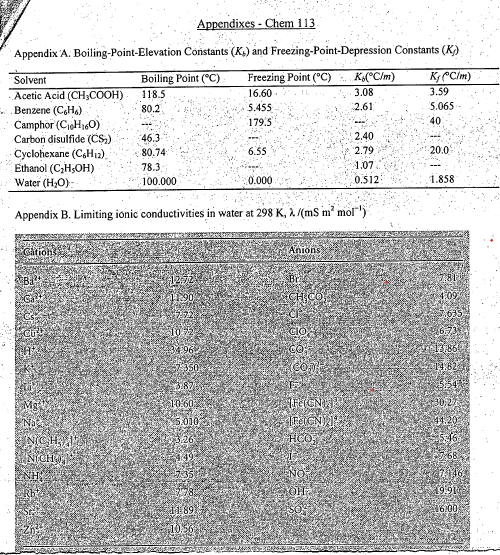
\includegraphics[width=0.75\textwidth, keepaspectratio]{images/151.png}
\end{center}

\begin{tcolorbox}[enhanced,breakable,ansbox,colback=cA!4,colframe=cA,boxrule=0.8pt,arc=5pt,title={\textbf{Answer}},fonttitle=\bfseries\color{white},colbacktitle=cA]
\textbf{Molar Conductivity and Acidity Constant of a Weak Acid:}

For a weak acid HA, the degree of dissociation $\alpha$ at
concentration $c$ is:
\[
  \alpha = \frac{\Lambda_m}{\Lambda_m^\circ}
\]
and the acidity constant is:
\[
  K_a = \frac{\alpha^2 c}{1 - \alpha}
\]

\bigskip
\textbf{Given:}
\begin{itemize}
  \item Concentration: $c = 0.010$ M
  \item Molar conductivity:
        $\Lambda_m = 1.65$ mS$\cdot$m$^2\cdot$mol$^{-1}$
  \item From Appendix B (limiting ionic conductivities at
        298 K):
        \[
          \lambda^\circ(\text{H}^+) = 34.96
          \text{ mS$\cdot$m}^2\cdot\text{mol}^{-1}
        \]
        \[
          \lambda^\circ(\text{CH}_3\text{COO}^-)
          = 4.09
          \text{ mS$\cdot$m}^2\cdot\text{mol}^{-1}
        \]
\end{itemize}

\bigskip
\textbf{(i) Limiting Molar Conductivity of CH$_3$COOH:}

By \textbf{Kohlrausch's Law of Independent Migration of Ions}:
\[
  \Lambda_m^\circ(\text{CH}_3\text{COOH})
  = \lambda^\circ(\text{H}^+)
  + \lambda^\circ(\text{CH}_3\text{COO}^-)
\]
\[
  = 34.96 + 4.09
\]
\[
  \boxed{\Lambda_m^\circ(\text{CH}_3\text{COOH})
  = 39.05 \text{ mS$\cdot$m}^2\cdot\text{mol}^{-1}}
\]

\bigskip
\textbf{(ii) Degree of Deprotonation $\alpha$:}
\[
  \alpha = \frac{\Lambda_m}{\Lambda_m^\circ}
         = \frac{1.65}{39.05}
\]
\[
  \boxed{\alpha = 0.04226 \approx 0.0423}
\]
This means only about \textbf{4.23\%} of CH$_3$COOH is
dissociated at 0.010 M — consistent with it being a weak acid.

\bigskip
\textbf{(iii) Acidity Constant $K_a$:}

The dissociation equilibrium:
\[
  \text{CH}_3\text{COOH}
  \rightleftharpoons
  \text{CH}_3\text{COO}^- + \text{H}^+
\]

\begin{center}
\begin{tabular}{p{3.5cm} p{2cm} p{2cm} p{2cm}}
\toprule
 & CH$_3$COOH & CH$_3$COO$^-$ & H$^+$ \\
\midrule
Initial (M)    & $c$         & 0            & 0 \\[3pt]
At equil.\ (M) & $c(1-\alpha)$ & $c\alpha$ & $c\alpha$ \\
\bottomrule
\end{tabular}
\end{center}

\[
  K_a = \frac{[\text{CH}_3\text{COO}^-][\text{H}^+]}
             {[\text{CH}_3\text{COOH}]}
      = \frac{(c\alpha)(c\alpha)}{c(1-\alpha)}
      = \frac{c\alpha^2}{1-\alpha}
\]
\[
  K_a = \frac{0.010 \times (0.04226)^2}{1 - 0.04226}
      = \frac{0.010 \times 1.786 \times 10^{-3}}{0.9577}
      = \frac{1.786 \times 10^{-5}}{0.9577}
\]
\[
  \boxed{K_a = 1.865 \times 10^{-5}
  \approx 1.86 \times 10^{-5}}
\]

This is close to the literature value for acetic acid
($K_a = 1.8 \times 10^{-5}$), confirming the method.

\bigskip
\textbf{Summary:}
\begin{center}
\begin{tabular}{p{5cm} p{4cm}}
\toprule
\textbf{Quantity} & \textbf{Value} \\
\midrule
$\Lambda_m^\circ$(CH$_3$COOH)
  & $39.05$ mS$\cdot$m$^2\cdot$mol$^{-1}$ \\[3pt]
Degree of deprotonation $\alpha$
  & $0.0423$ (4.23\%) \\[3pt]
Acidity constant $K_a$
  & $1.86 \times 10^{-5}$ \\
\bottomrule
\end{tabular}
\end{center}

\textbf{Conclusion:} Molar conductivity data provides a simple
and accurate route to $K_a$ of weak acids — the limiting molar
conductivity (from Kohlrausch's Law) gives $\Lambda_m^\circ$,
from which $\alpha$ and hence $K_a$ are directly calculated.
\end{tcolorbox}

\item What is meant by limiting ionic conductivity? Explain why the limiting ionic conductivity of H$^+$ is so high compared to other cations. \mk{7}
\yr{CHEM 113 | 2015--16}

\begin{tcolorbox}[enhanced,breakable,ansbox,colback=cA!4,colframe=cA,boxrule=0.8pt,arc=5pt,title={\textbf{Answer}},fonttitle=\bfseries\color{white},colbacktitle=cA]
\textbf{Limiting Ionic Conductivity ($\lambda^\circ$):}

The \textbf{limiting (or molar) ionic conductivity} is the
contribution of a single ion to the total molar conductivity
of an electrolyte at \textbf{infinite dilution} — i.e.\ when
ion--ion interactions are completely absent:
\[
  \Lambda_m^\circ
  = \nu_+\lambda_+^\circ + \nu_-\lambda_-^\circ
\]
(Kohlrausch's Law of Independent Migration)

At infinite dilution, each ion migrates independently,
and $\lambda^\circ$ represents the maximum conductivity
that ion can achieve. It is measured in
S$\cdot$m$^2\cdot$mol$^{-1}$.

\bigskip
\textbf{Why H$^+$ Has Exceptionally High $\lambda^\circ$:}

From Appendix B (298 K):
\[
  \lambda^\circ(\text{H}^+) = 34.96
  \text{ mS$\cdot$m}^2\text{mol}^{-1}
\]
Compare with other cations:
\[
  \lambda^\circ(\text{Na}^+) = 5.01, \quad
  \lambda^\circ(\text{K}^+)  = 7.35, \quad
  \lambda^\circ(\text{Li}^+) = 3.87
\]
H$^+$ is \textbf{5--9 times} more mobile than typical
cations.

\textbf{Explanation — Grotthuss Mechanism:}

Unlike ordinary ions which physically migrate through the
solvent (limited by Stokes drag and viscosity), H$^+$
conducts via a \textbf{proton-hopping relay} through the
hydrogen-bonded network of water:

\begin{center}
\begin{tikzpicture}[x=1.2cm, y=0.9cm]

  %% Step 1
  \node[font=\scriptsize\bfseries] at (-0.5,3.5)
    {Before:};
  \foreach \x/\label in {
    0/{H$_3$O$^+$}, 1.8/{H$_2$O},
    3.6/{H$_2$O}, 5.4/{H$_2$O}}{
    \draw[thick, blue!50] (\x,3.0) circle (0.4);
    \node[font=\tiny] at (\x,3.0) {\label};
  }
  \foreach \x in {0.4, 2.2, 4.0}{
    \draw[dashed, gray!50, thick] (\x,3.0)
      -- (\x+1.0,3.0);
  }

  %% Arrow showing time
  \draw[->, very thick, gray!50] (2.7,2.3)
    -- (2.7,1.8);

  %% Step 2
  \node[font=\scriptsize\bfseries] at (-0.5,1.3)
    {After:};
  \foreach \x/\label in {
    0/{H$_2$O}, 1.8/{H$_3$O$^+$},
    3.6/{H$_2$O}, 5.4/{H$_2$O}}{
    \draw[thick, blue!50] (\x,1.0) circle (0.4);
    \node[font=\tiny] at (\x,1.0) {\label};
  }
  \foreach \x in {0.4, 2.2, 4.0}{
    \draw[dashed, gray!50, thick] (\x,1.0)
      -- (\x+1.0,1.0);
  }

  %% Net proton movement arrow
  \draw[->, very thick, red!60] (0,0.0)
    -- (2.2,0.0);
  \node[below, font=\scriptsize, red!60] at (1.1,-0.1)
    {Net H$^+$ displacement};

\end{tikzpicture}
\end{center}

\begin{itemize}
  \item A proton hops from H$_3$O$^+$ to adjacent
        H$_2$O via a shared hydrogen bond
  \item The next H$_2$O reorients and passes the
        proton along the chain
  \item The \textbf{proton defect} propagates through
        the network at near-diffusion-limited speed
  \item No single proton travels far — the
        \textbf{information} (charge) travels rapidly
  \item This is far faster than Stokes diffusion
        of a classical ion of any size
\end{itemize}

\textbf{Conclusion:} Limiting ionic conductivity is the
maximum ionic contribution to molar conductivity at zero
concentration. H$^+$ has an exceptionally high
$\lambda^\circ = 34.96$ mS$\cdot$m$^2$mol$^{-1}$ because
it conducts via the \textbf{Grotthuss proton-hopping
mechanism} through hydrogen-bonded water — far faster
than any physically migrating ion.
\end{tcolorbox}

\item State Kohlrausch's law and Ostwald's dilution law. How can you use these two equations to determine the limiting values of the molar conductivity of solutions? \mk{9}
\yr{CHEM 113 | 2014--15}

\begin{tcolorbox}[enhanced,breakable,ansbox,colback=cA!4,colframe=cA,boxrule=0.8pt,arc=5pt,title={\textbf{Answer}},fonttitle=\bfseries\color{white},colbacktitle=cA]
\textbf{1. Kohlrausch's Law of Independent Migration of Ions:}

At infinite dilution, each ion migrates independently of
its co-ions. The limiting molar conductivity is:
\[
  \Lambda_m^\circ
  = \nu_+\lambda_+^\circ + \nu_-\lambda_-^\circ
\]
where $\nu_+$, $\nu_-$ are the stoichiometric numbers and
$\lambda_+^\circ$, $\lambda_-^\circ$ are the limiting ionic
conductivities.

For a 1:1 electrolyte:
\[
  \Lambda_m^\circ = \lambda_+^\circ + \lambda_-^\circ
\]

\textbf{Kohlrausch's empirical equation} for strong
electrolytes:
\[
  \Lambda_m = \Lambda_m^\circ - K\sqrt{c}
\]
where $K$ is a constant depending on the electrolyte type
and solvent. A plot of $\Lambda_m$ vs $\sqrt{c}$ gives a
straight line — extrapolation to $c = 0$ gives
$\Lambda_m^\circ$.

\bigskip
\textbf{2. Ostwald's Dilution Law:}

For a weak electrolyte (degree of dissociation $\alpha$):
\[
  K_a = \frac{\alpha^2 c}{1 - \alpha}
\]
Since $\alpha = \Lambda_m / \Lambda_m^\circ$:
\[
  K_a = \frac{(\Lambda_m/\Lambda_m^\circ)^2 \cdot c}
             {1 - \Lambda_m/\Lambda_m^\circ}
      = \frac{\Lambda_m^2 \cdot c}
             {\Lambda_m^\circ(\Lambda_m^\circ
             - \Lambda_m)}
\]
This is \textbf{Ostwald's Dilution Law} in conductance
form.

\bigskip
\textbf{3. Determining $\Lambda_m^\circ$ Using Both Laws:}

\textbf{For strong electrolytes} (e.g.\ KCl, NaCl):
\begin{itemize}
  \item $\Lambda_m$ can be measured at several
        concentrations
  \item Plot $\Lambda_m$ vs $\sqrt{c}$ (Kohlrausch)
  \item Extrapolate to $c = 0$ to obtain
        $\Lambda_m^\circ$ directly
\end{itemize}

\textbf{For weak electrolytes} (e.g.\ CH$_3$COOH):
\begin{itemize}
  \item Direct extrapolation fails — curve is non-linear
        and steep at low $c$
  \item Instead, use \textbf{Kohlrausch's Law} indirectly:
        \[
          \Lambda_m^\circ(\text{CH}_3\text{COOH})
          = \Lambda_m^\circ(\text{HCl})
          + \Lambda_m^\circ(\text{CH}_3\text{COONa})
          - \Lambda_m^\circ(\text{NaCl})
        \]
  \item Each term on the right can be obtained by
        extrapolation (all are strong electrolytes)
  \item Then use \textbf{Ostwald's Law} to find $\alpha$
        and $K_a$ at any concentration:
        \[
          \alpha = \frac{\Lambda_m}{\Lambda_m^\circ}
          \qquad
          K_a = \frac{\alpha^2 c}{1-\alpha}
        \]
\end{itemize}

\bigskip
\textbf{Graphical Method:}

\begin{center}
\begin{tikzpicture}[x=2.5cm, y=1.5cm]
  \draw[->, thick] (0,0) -- (2.2,0)
    node[right, font=\small] {$\sqrt{c}$};
  \draw[->, thick] (0,0) -- (0,3.5)
    node[above, font=\small] {$\Lambda_m$};

  %% Strong electrolyte line
  \draw[blue!70!black, very thick]
    plot coordinates {
      (0.3,3.0)(0.7,2.7)(1.1,2.4)(1.5,2.1)(1.9,1.8)
    };
  \draw[blue!60!black, dashed]
    plot coordinates {(0.3,3.0)(0.0,3.2)};
  \filldraw[blue!70!black] (0,3.2) circle (2.5pt);
  \node[left, font=\scriptsize, blue!70!black] at (0,3.2)
    {$\Lambda_m^\circ$ (strong)};
  \node[right, font=\scriptsize, blue!70!black] at (1.3,2.2)
    {Strong electrolyte};

  %% Weak electrolyte curve (steep, non-linear)
  \draw[red!70!black, very thick]
    plot[smooth] coordinates {
      (0.3,1.0)(0.6,0.8)(1.0,0.65)
      (1.4,0.55)(1.8,0.48)
    };
  \node[right, font=\scriptsize, red!70!black] at (1.4,0.45)
    {Weak electrolyte};
  \node[right, font=\scriptsize, red!60!black] at (0.3,0.75)
    {(extrapolation {\shortstack[l]unreliable})};

  %% Kohlrausch combination arrow
  \node[font=\tiny, align=center, gray] at (1.0,3.5)
    {Use Kohlrausch combination\\for weak electrolyte};

\end{tikzpicture}
\end{center}

\textbf{Conclusion:} Kohlrausch's Law allows
$\Lambda_m^\circ$ to be obtained by linear extrapolation
for strong electrolytes, and by ionic combination for
weak electrolytes. Ostwald's Dilution Law then uses
$\Lambda_m^\circ$ to determine dissociation constants
from conductance measurements.
\end{tcolorbox}

\item For the reaction Ag(s) + $\frac{1}{2}$Cl$_2$(g) $\rightarrow$ AgCl(s), $E^\circ = 0.839$ V at 1000 K. If $a_{\text{Ag}} = a_{\text{AgCl}} = 1.00$ and $a_{\text{Cl}_2} = 0.77$, find the value of E. Is the reaction less favored under non-standard conditions? Justify from the values of $K$ and $\Delta G$. \mk{9}
\yr{CHEM 113 | 2013--14}

\begin{tcolorbox}[enhanced,breakable,ansbox,colback=cA!4,colframe=cA,boxrule=0.8pt,arc=5pt,title={\textbf{Answer}},fonttitle=\bfseries\color{white},colbacktitle=cA]
\textbf{Given:}
\begin{itemize}
  \item Reaction: Ag$_{(s)}$ + $\tfrac{1}{2}$Cl$_{2(g)}$
        $\rightarrow$ AgCl$_{(s)}$
  \item $E^\circ = 0.839$ V at 1000 K
  \item $a_{\text{Ag}} = 1.00$, $a_{\text{AgCl}} = 1.00$,
        $a_{\text{Cl}_2} = 0.77$
  \item $n = 1$, $R = 8.314$ J/mol$\cdot$K,
        $F = 96485$ C/mol
\end{itemize}

\bigskip
\textbf{Reaction quotient $Q$:}
\[
  Q = \frac{a_{\text{AgCl}}}
           {a_{\text{Ag}} \cdot a_{\text{Cl}_2}^{1/2}}
    = \frac{1.00}{1.00 \times (0.77)^{1/2}}
    = \frac{1.00}{0.8775}
    = 1.140
\]

\bigskip
\textbf{Nernst equation:}
\[
  E = E^\circ - \frac{RT}{nF}\ln Q
    = 0.839 - \frac{(8.314)(1000)}{(1)(96485)}\ln(1.140)
\]
\[
  = 0.839 - (0.08617)(0.1310)
  = 0.839 - 0.01129
\]
\[
  \boxed{E = 0.828 \text{ V}}
\]

\bigskip
\textbf{$\Delta G$ under non-standard conditions:}
\[
  \Delta G = -nFE
           = -(1)(96485)(0.828)
           = -79{,}890 \text{ J/mol}
\]
\[
  \boxed{\Delta G = -79.9 \text{ kJ/mol}}
\]

\textbf{Equilibrium constant $K$:}
\[
  \Delta G^\circ = -nFE^\circ
                = -(1)(96485)(0.839)
                = -80{,}951 \text{ J/mol}
                = -80.95 \text{ kJ/mol}
\]
\[
  K = e^{-\Delta G^\circ/RT}
    = e^{80950/(8.314 \times 1000)}
    = e^{9.734}
    = 1.68 \times 10^4
\]

\bigskip
\textbf{Is the reaction less favoured under non-standard
conditions?}

\begin{itemize}
  \item $E = 0.828$ V $< E^\circ = 0.839$ V:
        cell emf is \textbf{slightly reduced}
  \item $\Delta G = -79.9$ kJ/mol vs
        $\Delta G^\circ = -80.95$ kJ/mol: both are
        \textbf{negative} — reaction is spontaneous
        under both conditions
  \item $Q = 1.140 > 1$: the reaction has slightly
        less driving force than standard
  \item $K = 1.68 \times 10^4 \gg 1$: equilibrium
        lies far to the right — reaction strongly
        favoured
\end{itemize}

\textbf{Conclusion:} The reaction is \textbf{marginally
less favoured} under non-standard conditions ($E = 0.828$
V vs 0.839 V) because $a_{\text{Cl}_2} < 1$ reduces the
driving force slightly. However, the large negative
$\Delta G$ and very large $K$ confirm the reaction remains
\textbf{strongly spontaneous} and product-favoured.
\end{tcolorbox}

\item Define reversible cell. Give an example and explain how it is reversible. \mk{11}
\yr{CHEM 113 | 2011--12}

\begin{tcolorbox}[enhanced,breakable,ansbox,colback=cA!4,colframe=cA,boxrule=0.8pt,arc=5pt,title={\textbf{Answer}},fonttitle=\bfseries\color{white},colbacktitle=cA]
\textbf{Reversible Cell — Definition:}

A \textbf{reversible cell} is an electrochemical cell that operates under thermodynamically reversible conditions — meaning an infinitesimally small opposing EMF can reverse the direction of current flow and all associated chemical reactions, with no net energy dissipation.

\textbf{Conditions for reversibility:}
\begin{enumerate}
  \item The cell reaction must be \textbf{chemically reversible}: the exact reverse reaction occurs when current is reversed
  \item The cell must operate \textbf{infinitely slowly} (quasi-statically) — no current flows in the ideal limit
  \item \textbf{No irreversible processes}: no concentration polarisation, no side reactions
\end{enumerate}

\bigskip
\textbf{Example — Daniell Cell:}

The \textbf{Daniell cell} is the classic example:
$$
  \text{Zn}_{(s)} \,|\, \text{ZnSO}_{4(aq)} \,\|\, \text{CuSO}_{4(aq)} \,|\, \text{Cu}_{(s)}
$$

\textbf{Cell diagram and reactions:}

\begin{center}
\begin{tikzpicture}[>=stealth, font=\small]

  % --- Solutions ---
  % ZnSO4 Solution (Pale / Colorless)
  \fill[shade, top color=cyan!5, bottom color=cyan!15, fill opacity=0.8] (0.5, 0.2) rectangle (3.5, 3.0);
  \draw[cyan!40!black, thick] (0.5, 3.0) to[out=10, in=170] (3.5, 3.0); % Meniscus
  \node[font=\small\bfseries, text=cyan!80!black] at (1.5, 1.2) {ZnSO$_4$ (aq)};

  % CuSO4 Solution (Blue)
  \fill[shade, top color=blue!20, bottom color=blue!40, fill opacity=0.8] (5.5, 0.2) rectangle (8.5, 3.0);
  \draw[blue!60!black, thick] (5.5, 3.0) to[out=10, in=170] (8.5, 3.0); % Meniscus
  \node[font=\small\bfseries, text=blue!90!black] at (7.5, 1.2) {CuSO$_4$ (aq)};

  % --- Beakers ---
  \draw[thick, draw=black!60, rounded corners=4pt] (0.5, 3.8) -- (0.5, 0.2) -- (3.5, 0.2) -- (3.5, 3.8);
  \draw[thick, draw=black!60, rounded corners=4pt] (5.5, 3.8) -- (5.5, 0.2) -- (8.5, 0.2) -- (8.5, 3.8);

  % --- Electrodes ---
  % Zn Anode
  \fill[shade, left color=gray!30, right color=gray!50, draw=black!70, thick, rounded corners=1pt] (1.6, 0.5) rectangle (2.4, 4.5);
  \node[font=\small\bfseries, text=black!80] at (2.0, 2.3) {Zn};
  \node[font=\scriptsize\bfseries, text=black!80, align=center] at (2.0, -0.3) {Anode (--)};

  % Cu Cathode
  \fill[shade, left color=orange!40, right color=orange!70!black, draw=black!70, thick, rounded corners=1pt] (6.6, 0.5) rectangle (7.4, 4.5);
  \node[font=\small\bfseries, text=white] at (7.0, 2.3) {Cu};
  \node[font=\scriptsize\bfseries, text=black!80, align=center] at (7.0, -0.3) {Cathode (+)};

  % --- Salt Bridge ---
  \draw[thick, draw=black!60, fill=yellow!10, rounded corners=8pt]
      (2.8, 1.5) -- (2.8, 4.2) -- (6.2, 4.2) -- (6.2, 1.5) --
      (5.6, 1.5) -- (5.6, 3.6) -- (3.4, 3.6) -- (3.4, 1.5) -- cycle;
  % Plugs
  \fill[gray!40] (2.8, 1.5) rectangle (3.4, 1.7); % left plug
  \fill[gray!40] (5.6, 1.5) rectangle (6.2, 1.7); % right plug
  \node[font=\scriptsize\bfseries, text=black!70] at (4.5, 4.5) {Salt Bridge (KCl)};
  
  % Ion flow in bridge
  \draw[->, thick, red!70!black] (4.0, 3.9) -- (3.5, 3.9);
  \node[above, font=\tiny\bfseries, text=red!70!black] at (3.75, 3.9) {Cl$^-$};
  \draw[->, thick, blue!70!black] (5.0, 3.9) -- (5.5, 3.9);
  \node[above, font=\tiny\bfseries, text=blue!70!black] at (5.25, 3.9) {K$^+$};

  % --- External Circuit ---
  \draw[ultra thick, black!80] (2.0, 4.5) |- (4.0, 5.5);
  \draw[ultra thick, black!80] (7.0, 4.5) |- (5.0, 5.5);

  % Voltmeter
  \fill[shade, top color=gray!10, bottom color=gray!30, draw=black!80, thick] (4.5, 5.5) circle (0.5);
  \node[font=\large\bfseries, text=black] at (4.5, 5.5) {V};
  \node[font=\scriptsize\bfseries, text=black!80, fill=white, inner sep=1pt] at (4.5, 6.3) {1.10 V};

  % Electron Flow (Discharge)
  \draw[->, ultra thick, blue!80!black] (2.4, 5.7) -- (3.6, 5.7);
  \node[above, font=\scriptsize\bfseries, text=blue!80!black] at (3.0, 5.7) {$e^-$};
  \draw[->, ultra thick, blue!80!black] (5.4, 5.7) -- (6.6, 5.7);
  \node[above, font=\scriptsize\bfseries, text=blue!80!black] at (6.0, 5.7) {$e^-$};

  % Electrode Reactions
  \node[font=\scriptsize\bfseries, text=black!70, align=center] at (1.1, 2.0) {Zn $\rightarrow$ Zn$^{2+} + 2e^-$};
  \node[font=\scriptsize\bfseries, text=black!70, align=center] at (8.1, 2.0) {Cu$^{2+} + 2e^- \rightarrow$ Cu};

\end{tikzpicture}
\end{center}

\textbf{Discharge (forward):}
$$
  \text{Zn}_{(s)} \rightarrow \text{Zn}^{2+}_{(aq)} + 2e^- \quad \text{(oxidation, anode)}
$$
$$
  \text{Cu}^{2+}_{(aq)} + 2e^- \rightarrow \text{Cu}_{(s)} \quad \text{(reduction, cathode)}
$$
$$
  \text{Overall: } \text{Zn}_{(s)} + \text{Cu}^{2+}_{(aq)} \rightarrow \text{Zn}^{2+}_{(aq)} + \text{Cu}_{(s)} \quad E^\circ = 1.10 \text{ V}
$$

\textbf{Charging (reverse — applying external EMF $> 1.10$ V):}
$$
  \text{Zn}^{2+}_{(aq)} + 2e^- \rightarrow \text{Zn}_{(s)} \quad \text{(reduction)}
$$
$$
  \text{Cu}_{(s)} \rightarrow \text{Cu}^{2+}_{(aq)} + 2e^- \quad \text{(oxidation)}
$$

The \textbf{exact chemical reverse} occurs — confirming reversibility. The cell is reversible because:
\begin{itemize}
  \item Both electrode reactions are thermodynamically reversible (metal/metal ion couples)
  \item The salt bridge maintains electrical neutrality without irreversible mixing
  \item Applying a slightly larger EMF exactly reverses all processes
\end{itemize}

\textbf{Conclusion:} A reversible cell operates under equilibrium conditions where the cell reaction and its exact reverse can occur by infinitesimal changes in the applied EMF. The Daniell cell exemplifies reversibility — its forward and reverse reactions are chemically and thermodynamically identical in magnitude.
\end{tcolorbox}

\item Establish a relation between the emf of a reversible cell and the heat of reaction in the cell. \mk{14}
\yr{CHEM 113 | 2011--12}

\begin{tcolorbox}[enhanced,breakable,ansbox,colback=cA!4,colframe=cA,boxrule=0.8pt,arc=5pt,title={\textbf{Answer}},fonttitle=\bfseries\color{white},colbacktitle=cA]
\textbf{Relation Between EMF and Heat of Reaction —
Gibbs--Helmholtz Equation:}

\textbf{Step 1 — EMF and Gibbs free energy:}

For a reversible cell doing electrical work:
\[
  \Delta G = -nFE
\]
where $n$ = moles of electrons, $F$ = Faraday constant,
$E$ = EMF.

\textbf{Step 2 — Temperature dependence of $\Delta G$:}

From the Gibbs--Helmholtz equation:
\[
  \Delta G = \Delta H + T\left(\frac{\partial \Delta G}
             {\partial T}\right)_P
\]

Substituting $\Delta G = -nFE$:
\[
  -nFE = \Delta H
  + T\left(\frac{\partial(-nFE)}{\partial T}\right)_P
\]
\[
  -nFE = \Delta H - nFT\left(\frac{\partial E}
         {\partial T}\right)_P
\]

Rearranging:
\[
  \boxed{
    \Delta H = -nFE + nFT\left(\frac{\partial E}
               {\partial T}\right)_P
    = -nF\left[E - T\left(\frac{\partial E}
      {\partial T}\right)_P\right]
  }
\]

This is the \textbf{Gibbs--Helmholtz equation} for a cell.

\textbf{Step 3 — Physical interpretation:}

\begin{itemize}
  \item $-nFE = \Delta G$: electrical energy (free energy)
  \item $nFT(\partial E/\partial T)_P = T\Delta S$:
        heat exchanged reversibly with surroundings
  \item Therefore: $\Delta H = \Delta G + T\Delta S$
        (first law, as expected)
\end{itemize}

\textbf{Three cases:}
\begin{enumerate}
  \item $\left(\frac{\partial E}{\partial T}\right)_P > 0$:
        cell absorbs heat from surroundings
        ($\Delta H < \Delta G$, endothermic)
  \item $\left(\frac{\partial E}{\partial T}\right)_P = 0$:
        $\Delta H = \Delta G = -nFE$ (no heat exchange)
  \item $\left(\frac{\partial E}{\partial T}\right)_P < 0$:
        cell evolves heat to surroundings
        ($\Delta H > \Delta G$, exothermic)
\end{enumerate}

\textbf{Entropy of cell reaction:}
\[
  \Delta S = nF\left(\frac{\partial E}{\partial T}\right)_P
\]

\textbf{Conclusion:} The heat of reaction in a reversible
cell is related to EMF by:
\[
  \Delta H = -nF\left[E - T\left(\frac{\partial E}
             {\partial T}\right)_P\right]
\]
This shows that $\Delta H \neq -nFE$ unless
$(\partial E/\partial T)_P = 0$. The temperature
coefficient of EMF captures the entropy contribution,
allowing complete thermodynamic characterisation of cell
reactions from electrical measurements alone.
\end{tcolorbox}

\item At 25$^\circ$C the value of the emf for the reversible cell: Pb, PbCl$_2$(s)$|$KCl(aq)$|$AgCl(s), Ag is 0.4902 volt and $(\partial E / \partial T)_p = -1.86 \times 10^{-4}$ volt$\cdot$deg$^{-1}$. Calculate the values of $\Delta G$ and $\Delta H$ showing the reaction involved in the cell. \mk{10}
\yr{CHEM 113 | 2011--12}

\begin{tcolorbox}[enhanced,breakable,ansbox,colback=cA!4,colframe=cA,boxrule=0.8pt,arc=5pt,title={\textbf{Answer}},fonttitle=\bfseries\color{white},colbacktitle=cA]
\textbf{Given:}
\begin{itemize}
  \item Cell: Pb, PbCl$_2$(s) $|$ KCl(aq) $|$
        AgCl(s), Ag
  \item $E = 0.4902$ V at $T = 25^\circ$C $= 298$ K
  \item $(\partial E/\partial T)_P
        = -1.86 \times 10^{-4}$ V$\cdot$deg$^{-1}$
  \item $n = 2$ (two electrons transferred)
  \item $F = 96485$ C/mol
\end{itemize}

\textbf{Cell reaction:}
\[
  \text{Pb}_{(s)} + 2\text{AgCl}_{(s)}
  \rightarrow \text{PbCl}_{2(s)} + 2\text{Ag}_{(s)}
\]

\bigskip
\textbf{Calculate $\Delta G$:}
\[
  \Delta G = -nFE
           = -(2)(96485)(0.4902)
           = -94{,}574 \text{ J/mol}
\]
\[
  \boxed{\Delta G = -94.57 \text{ kJ/mol}}
\]

\bigskip
\textbf{Calculate $\Delta H$:}

Using the Gibbs--Helmholtz equation:
\[
  \Delta H
  = -nF\left[E - T\left(\frac{\partial E}
    {\partial T}\right)_P\right]
\]
\[
  = -(2)(96485)\left[0.4902
    - (298)(-1.86\times10^{-4})\right]
\]
\[
  = -(2)(96485)\left[0.4902 + 0.05543\right]
\]
\[
  = -(2)(96485)(0.5456)
\]
\[
  = -105{,}274 \text{ J/mol}
\]
\[
  \boxed{\Delta H = -105.27 \text{ kJ/mol}}
\]

\bigskip
\textbf{Calculate $\Delta S$:}
\[
  \Delta S = nF\left(\frac{\partial E}{\partial T}\right)_P
           = (2)(96485)(-1.86\times10^{-4})
           = -35.91 \text{ J/mol$\cdot$K}
\]

\textbf{Verification:}
\[
  \Delta H = \Delta G + T\Delta S
           = -94{,}574 + (298)(-35.91)
           = -94{,}574 - 10{,}701
           = -105{,}275 \text{ J/mol} \quad\checkmark
\]

\bigskip
\textbf{Summary:}
\begin{center}
\begin{tabular}{p{3cm} p{5cm}}
\toprule
\textbf{Quantity} & \textbf{Value} \\
\midrule
$\Delta G$ & $-94.57$ kJ/mol (spontaneous) \\[3pt]
$\Delta H$ & $-105.27$ kJ/mol (exothermic) \\[3pt]
$\Delta S$ & $-35.91$ J/mol$\cdot$K (order increases) \\
\bottomrule
\end{tabular}
\end{center}

\textbf{Conclusion:} The cell reaction is both
spontaneous ($\Delta G < 0$) and exothermic
($\Delta H < 0$). The negative $\Delta S$ indicates
increased order (forming solid PbCl$_2$ and Ag from
Pb and AgCl).
\end{tcolorbox}

\item What are reversible and irreversible cells? Give one example of each. \mk{3}
\yr{CHEM 101 | 2009--10}

\begin{tcolorbox}[enhanced,breakable,ansbox,colback=cA!4,colframe=cA,boxrule=0.8pt,arc=5pt,title={\textbf{Answer}},fonttitle=\bfseries\color{white},colbacktitle=cA]
\textbf{Reversible Cell:}

A cell in which the electrode reactions can be
\textbf{exactly reversed} by applying an infinitesimally
larger opposing EMF, with all chemical changes being
perfectly reversible.

\textbf{Example:} Daniell cell:
\[
  \text{Zn} | \text{ZnSO}_4 \| \text{CuSO}_4 | \text{Cu}
  \qquad E^\circ = 1.10 \text{ V}
\]

\bigskip
\textbf{Irreversible Cell:}

A cell in which the electrode reactions \textbf{cannot be
simply reversed} — applying a reverse EMF produces
different reactions or the same electrode is not restored.

\textbf{Example:} Grove cell or a cell with Zn in HCl:
\[
  \text{Zn}_{(s)} + 2\text{HCl}_{(aq)}
  \rightarrow \text{ZnCl}_{2(aq)} + \text{H}_{2(g)}
\]
Passing current in reverse does not regenerate Zn and HCl
in the same proportions — irreversible.

\begin{center}
\begin{tabular}{p{3cm} p{3cm} p{3cm}}
\toprule
\textbf{Feature} & \textbf{Reversible} &
\textbf{Irreversible} \\
\midrule
Reaction reversal & Exact reverse & Different products \\
Thermodynamic treatment & Possible & Not applicable \\
EMF & Well-defined & Variable \\
Example & Daniell cell & Zn/HCl cell \\
\bottomrule
\end{tabular}
\end{center}
\end{tcolorbox}

\item State the Kohlrausch law of independent migration of ions. Discuss its applications. \mk{9}
\yr{CHEM 101 | 2009--10}

\begin{tcolorbox}[enhanced,breakable,ansbox,colback=cA!4,colframe=cA,boxrule=0.8pt,arc=5pt,title={\textbf{Answer}},fonttitle=\bfseries\color{white},colbacktitle=cA]
\textbf{Kohlrausch's Law of Independent Migration of Ions:}

\textbf{Statement:} At infinite dilution, each ion
migrates independently of all other ions, and contributes
a fixed, characteristic amount to the total molar
conductivity of the electrolyte, regardless of the
nature of the co-ion:
\[
  \Lambda_m^\circ
  = \nu_+\lambda_+^\circ + \nu_-\lambda_-^\circ
\]

\textbf{Applications:}

\begin{enumerate}
  \item \textbf{Finding $\Lambda_m^\circ$ of weak
        electrolytes:}\\
        Direct extrapolation impossible for weak
        electrolytes. Use combination:
        \[
          \Lambda_m^\circ(\text{CH}_3\text{COOH})
          = \Lambda_m^\circ(\text{HCl})
          + \Lambda_m^\circ(\text{CH}_3\text{COONa})
          - \Lambda_m^\circ(\text{NaCl})
        \]

  \item \textbf{Degree of dissociation:}
        \[
          \alpha = \frac{\Lambda_m}{\Lambda_m^\circ}
        \]

  \item \textbf{Dissociation constant:}
        \[
          K_a = \frac{\alpha^2 c}{1-\alpha}
              = \frac{\Lambda_m^2 c}
                     {\Lambda_m^\circ
                     (\Lambda_m^\circ - \Lambda_m)}
        \]

  \item \textbf{Ionic mobilities:}
        Individual $\lambda^\circ$ values directly
        give ionic mobilities:
        $u_i = \lambda_i^\circ / F$

  \item \textbf{Transport numbers:}
        \[
          t_+ = \frac{\lambda_+^\circ}
                     {\lambda_+^\circ + \lambda_-^\circ},
          \qquad
          t_- = \frac{\lambda_-^\circ}
                     {\lambda_+^\circ + \lambda_-^\circ}
        \]

  \item \textbf{Solubility of sparingly soluble salts:}
        $\kappa_{\text{solution}} - \kappa_{\text{water}}
        = \Lambda_m^\circ \cdot c_{\text{sat}}$
        gives solubility $c_{\text{sat}}$
\end{enumerate}

\textbf{Conclusion:} Kohlrausch's Law is foundational to
electrolyte chemistry — it allows calculation of limiting
molar conductivities, dissociation constants, ionic
mobilities, and solubility products from simple
conductance measurements.
\end{tcolorbox}

\item Briefly discuss the chronological development of the mechanism of electrolytic conduction. \mk{8}
\yr{CHEM 101 | 2008--09}

\begin{tcolorbox}[enhanced,breakable,ansbox,colback=cA!4,colframe=cA,boxrule=0.8pt,arc=5pt,title={\textbf{Answer}},fonttitle=\bfseries\color{white},colbacktitle=cA]
\textbf{Chronological Development of Electrolytic
Conduction Mechanism:}

\begin{enumerate}
  \item \textbf{Faraday (1833--1834) — Laws of
        Electrolysis:}\\
        Michael Faraday established that electricity
        passed through solutions causes chemical
        decomposition (\textbf{electrolysis}). He
        introduced the terms \textit{electrolyte,
        electrode, anode, cathode, ion}. His laws showed
        that the amount of substance deposited is
        proportional to the charge passed — implying
        discrete charged particles (ions) carry current.

  \item \textbf{Hittorf (1853) — Transport Numbers:}\\
        Hittorf showed that cations and anions migrate
        independently and carry different fractions of
        current. He introduced the concept of
        \textbf{transport numbers} ($t_+$, $t_-$),
        measured by changes in electrode compartment
        concentrations.

  \item \textbf{Kohlrausch (1874--1885) — Conductance
        Measurements:}\\
        Kohlrausch made precise conductance measurements
        using AC current (avoiding electrolysis) and
        showed: $\Lambda_m = \Lambda_m^\circ - K\sqrt{c}$.
        He established the \textbf{law of independent
        migration} — each ion has a characteristic
        limiting conductivity.

  \item \textbf{Arrhenius (1887) — Ionic Dissociation
        Theory:}\\
        Arrhenius proposed that electrolytes
        \textbf{spontaneously dissociate} into ions in
        solution — even without current. He used
        conductance data to calculate degree of
        dissociation $\alpha = \Lambda_m/\Lambda_m^\circ$.
        This explained anomalous colligative properties.

  \item \textbf{Ostwald (1888) — Dilution Law:}\\
        Ostwald confirmed Arrhenius's theory for weak
        electrolytes:
        $K_a = \alpha^2 c/(1-\alpha)$. His dilution
        law quantitatively described partial dissociation.

  \item \textbf{Debye and Hückel (1923) — Ion Atmosphere
        Theory:}\\
        For strong electrolytes (fully dissociated at
        all concentrations), Debye and Hückel explained
        the \textbf{decrease of conductance with
        concentration} through the concept of the
        \textbf{ionic atmosphere} — each ion is
        surrounded by a cloud of opposite charges that:
        \begin{itemize}
          \item \textbf{Relaxation effect}: the ionic
                atmosphere takes time to reorganise when
                an ion moves, creating a retarding force
          \item \textbf{Electrophoretic effect}: the
                solvent molecules dragged by the
                oppositely charged atmosphere oppose the
                ion's motion
        \end{itemize}
        Their theory predicted $\Lambda_m = \Lambda_m^\circ
        - K\sqrt{c}$ — identical in form to Kohlrausch's
        empirical law.

  \item \textbf{Onsager (1927) — Extended Theory:}\\
        Onsager provided the rigorous mathematical
        treatment of the Debye--Hückel conductance
        theory, deriving the limiting law coefficient
        $K$ from first principles.
\end{enumerate}

\textbf{Conclusion:} The understanding of electrolytic
conduction evolved from Faraday's empirical laws through
Arrhenius's ionic dissociation theory to the rigorous
Debye--Hückel--Onsager theory — transforming a
phenomenological description into a quantitative
molecular theory of ion--ion interactions in solution.
\end{tcolorbox}

\item Define transport number. Show that $t_+ + t_- = 1.0$. \mk{4}
\yr{CHEM 101 | 2008--09}

\begin{tcolorbox}[enhanced,breakable,ansbox,colback=cA!4,colframe=cA,boxrule=0.8pt,arc=5pt,title={\textbf{Answer}},fonttitle=\bfseries\color{white},colbacktitle=cA]
\textbf{Transport Number — Definition:}

The \textbf{transport number} (transference number) $t_i$
of an ion is the fraction of the total current carried
by that ion:
\[
  t_i = \frac{I_i}{I_{\text{total}}}
      = \frac{\text{current carried by ion }i}
             {\text{total current}}
\]

For a binary electrolyte:
\[
  t_+ = \frac{u_+}{u_+ + u_-}
  \qquad
  t_- = \frac{u_-}{u_+ + u_-}
\]
where $u_+$ and $u_-$ are ionic mobilities.

\bigskip
\textbf{Proof that $t_+ + t_- = 1$:}

The total current in solution is the sum of currents
carried by cations and anions:
\[
  I_{\text{total}} = I_+ + I_-
\]

By definition:
\[
  t_+ + t_-
  = \frac{I_+}{I_{\text{total}}}
  + \frac{I_-}{I_{\text{total}}}
  = \frac{I_+ + I_-}{I_{\text{total}}}
  = \frac{I_{\text{total}}}{I_{\text{total}}}
\]
\[
  \boxed{t_+ + t_- = 1}
\]

Alternatively, using mobilities directly:
\[
  t_+ + t_-
  = \frac{u_+}{u_+ + u_-}
  + \frac{u_-}{u_+ + u_-}
  = \frac{u_+ + u_-}{u_+ + u_-}
  = 1 \quad\checkmark
\]

\textbf{Note:} For a multicomponent electrolyte:
$\sum_i t_i = 1$ (all ions together carry 100\% of
current).

\textbf{Example} (HCl at 298 K, from Appendix B):
\[
  t_+ = \frac{34.96}{34.96 + 7.63} = 0.821
  \qquad
  t_- = \frac{7.63}{34.96 + 7.63} = 0.179
\]
\[
  t_+ + t_- = 0.821 + 0.179 = 1.000 \quad\checkmark
\]
\end{tcolorbox}

\item Explain the terms: conductance, specific conductance, equivalent conductance, and molecular conductance. Derive a relation between specific conductance and equivalent conductance. \mk{15}
\yr{CHEM 101 | 2007--08}

\begin{tcolorbox}[enhanced,breakable,ansbox,colback=cA!4,colframe=cA,boxrule=0.8pt,arc=5pt,title={\textbf{Answer}},fonttitle=\bfseries\color{white},colbacktitle=cA]
\textbf{1. Conductance ($G$):}

The \textbf{conductance} of a solution is the reciprocal
of its electrical resistance:
\[
  G = \frac{1}{R} \qquad \text{(unit: siemens, S)}
\]
It measures the ease with which current flows through the
solution between two electrodes.

\bigskip
\textbf{2. Specific Conductance ($\kappa$):}

The \textbf{specific conductance} (conductivity) is the
conductance of a solution contained between two electrodes
of unit area ($A = 1$ cm$^2$) separated by unit distance
($l = 1$ cm):
\[
  \kappa = G \times \frac{l}{A}
         = G \times \text{cell constant}
\]
Units: S$\cdot$cm$^{-1}$ or S$\cdot$m$^{-1}$.

It is an intrinsic property of the solution (independent
of cell geometry).

\bigskip
\textbf{3. Equivalent Conductance ($\Lambda_{\text{eq}}$):}

The \textbf{equivalent conductance} is the conductance of
a solution containing \textbf{one equivalent of electrolyte}
placed between two electrodes 1 cm apart:
\[
  \Lambda_{\text{eq}}
  = \frac{\kappa \times 1000}{N}
\]
where $N$ is the normality (equivalents/L) and 1000
converts L to cm$^3$.

Units: S$\cdot$cm$^2\cdot$eq$^{-1}$.

\bigskip
\textbf{4. Molecular (Molar) Conductance ($\Lambda_m$):}

The \textbf{molar conductance} is the conductance of a
solution containing \textbf{one mole of electrolyte}
between electrodes 1 cm apart:
\[
  \Lambda_m = \frac{\kappa \times 1000}{M}
\]
where $M$ is the molarity (mol/L).

Units: S$\cdot$cm$^2\cdot$mol$^{-1}$.

For a 1:1 electrolyte: $\Lambda_m = \Lambda_{\text{eq}}$.
For a 2:1 electrolyte (e.g.\ CaCl$_2$):
$\Lambda_m = 2\Lambda_{\text{eq}}$.

\bigskip
\textbf{Relation Between $\kappa$ and $\Lambda_{\text{eq}}$:}

Consider 1 L of solution of normality $N$.
Number of equivalents $= N$.
Volume containing 1 equivalent $= 1000/N$ cm$^3$.

If this volume is placed between electrodes of area $A$
separated by $l$:
\[
  \Lambda_{\text{eq}} = G \times 1
  \quad \text{(electrodes 1 cm apart, unit area)}
\]
\[
  G = \kappa \times \frac{A}{l}
  = \kappa \times \frac{1000/N}{1}
  \qquad \text{(when }l = 1, A = V = 1000/N\text{)}
\]

Therefore:
\[
  \boxed{
    \Lambda_{\text{eq}}
    = \frac{\kappa \times 1000}{N}
  }
\]

\textbf{Summary:}
\begin{center}
\begin{tabular}{p{3cm} p{4cm} p{2.5cm}}
\toprule
\textbf{Quantity} & \textbf{Definition} & \textbf{Units} \\
\midrule
$G$ (Conductance)
  & $1/R$
  & S \\[3pt]
$\kappa$ (Specific conductance)
  & $G \times l/A$
  & S$\cdot$cm$^{-1}$ \\[3pt]
$\Lambda_{\text{eq}}$ (Equiv. conductance)
  & $\kappa \times 1000 / N$
  & S$\cdot$cm$^2$eq$^{-1}$ \\[3pt]
$\Lambda_m$ (Molar conductance)
  & $\kappa \times 1000 / M$
  & S$\cdot$cm$^2$mol$^{-1}$ \\
\bottomrule
\end{tabular}
\end{center}
\end{tcolorbox}

\item Give a brief description of the lead storage cell. \mk{10}
\yr{CHEM 101 | 2007--08}

%%══════════════════════════════════════════════════════════════════════
%% S9 — Polymers
%%══════════════════════════════════════════════════════════════════════
\item What is an electrochemical cell? How do you understand the terms ``half cell'', ``half-cell reaction'' and ``salt bridge''? \mk{10}
\yr{CHEM 101 | 2006--07}

\begin{tcolorbox}[enhanced,breakable,ansbox,colback=cA!4,colframe=cA,boxrule=0.8pt,arc=5pt,title={\textbf{Answer}},fonttitle=\bfseries\color{white},colbacktitle=cA]
\textbf{Electrochemical Cell:}

An \textbf{electrochemical cell} is a device that converts
\textbf{chemical energy to electrical energy} (galvanic cell)
or \textbf{electrical energy to chemical energy}
(electrolytic cell) through redox reactions at two
electrodes.

\bigskip
\textbf{Half Cell:}

A \textbf{half cell} (or electrode) consists of a single
electrode in contact with a solution of its ions. It is
the site of either oxidation or reduction:
\begin{itemize}
  \item \textbf{Anode half cell}: oxidation occurs
        (e.g.\ Zn $|$ ZnSO$_4$ solution)
  \item \textbf{Cathode half cell}: reduction occurs
        (e.g.\ Cu $|$ CuSO$_4$ solution)
\end{itemize}

\textbf{Half-cell reaction:}

The individual oxidation or reduction reaction occurring
at one electrode:
\[
  \text{Zn} \rightarrow \text{Zn}^{2+} + 2e^-
  \quad \text{(oxidation, anode)}
\]
\[
  \text{Cu}^{2+} + 2e^- \rightarrow \text{Cu}
  \quad \text{(reduction, cathode)}
\]
The sum of two half-cell reactions gives the
\textbf{overall cell reaction}.

\bigskip
\textbf{Salt Bridge:}

A \textbf{salt bridge} is a U-shaped tube filled with a
concentrated solution of an inert electrolyte
(e.g.\ KCl, KNO$_3$ in agar gel) connecting the two
half cells. Its functions:
\begin{itemize}
  \item \textbf{Completes the electrical circuit} by
        allowing ion flow between the two solutions
  \item \textbf{Maintains electrical neutrality} — as
        Zn$^{2+}$ builds up in the anode compartment,
        Cl$^-$ ions migrate in; as Cu$^{2+}$ is depleted
        at the cathode, K$^+$ ions migrate in
  \item \textbf{Prevents direct mixing} of the two
        electrode solutions (which would cause direct
        chemical reaction and no electrical work)
  \item KCl is preferred because
        $t_+(\text{K}^+) \approx t_-(\text{Cl}^-)$,
        minimising the liquid junction potential
\end{itemize}

\begin{center}

  \begin{tikzpicture}[line join=round, line cap= round]
  % CELLS AND ELECTRODES
  \begin{scope}
    \draw[thick,fill=gray!50] (0.5,1) rectangle (1,5);    % Zn electrode
    \draw[thick,rounded corners] (0,4) |- (4,0) -- (4,4); % left cell
    \clip[rounded corners]       (0,4) |- (4,0) -- (4,4) -- cycle;
    \fill[gray,opacity=0.3]   (0,0)   rectangle (4,3);    % ZnSO4 solution
  \end{scope}
  \begin{scope}
    \draw[thick,fill=orange!50] (8,1) rectangle (8.5,5);  % Cu electrode
    \draw[thick,rounded corners] (5,4) |- (9,0) -- (9,4); % right cell
    \clip[rounded corners]       (5,4) |- (9,0) -- (9,4) -- cycle;
    \fill[blue, opacity=0.2]    (5,0) rectangle (9,3);    % CuSO4 solution
  \end{scope}
  % SALINE BRIDGE
  \draw[thick] (3,1)   --++ (0,2.5) arc (180:0:1.5) --++ (0,-2.5);
  \draw[thick] (3.5,1) --++ (0,2.5) arc (180:0:1)   --++ (0,-2.5);
  % WIRE AND VOLTMETER
  \draw[thick, rounded corners=0.5 cm] (0.75,5) |- (8.25,7) -- (8.25,5);
  \begin{scope}[shift={(4.5,7)}]
  \draw[thick,fill=white] (0,0) circle (0.5);
    \foreach\a in{30,60,...,150}
    {%
      \draw[blue,thin] (\a:0.35) -- (\a:0.45);
    }
  \fill[blue] (0,0) circle (1pt);
  \draw[blue,thick,-latex] (0,0) -- (60:0.4);
  \end{scope}
  % ELECTRONS
  \begin{scope}[shift={(1.5,6.25)}]
    \draw[red,thick,rounded corners=0.3 cm,->] (-0.5,-0.5) |- (0.5,0.5);
  \end{scope}
  % SIGNS
  \draw[red,thick] (-0.5,5.5) circle (0.25);
  \draw[red,thick] (9.5,5.5)  circle (0.25);
  \draw[red,thick] (-0.7,5.5) -- (-0.3,5.5);
  \draw[red,thick] (9.3,5.5)  -- (9.7,5.5);
  \draw[red,thick] (9.5,5.3)  -- (9.5,5.7);
  % LABELS
  \node at (4.5,8)    {Voltmeter};
  \node at (4.5,5.5)  {Saline bridge (\ce{KCl})};
  \node at (-0.5,5)   {Anode};
  \node at (-0.5,4.5) {(oxidation)};
  \node at (9.5,5)    {Cathode};
  \node at (9.5,4.5)  {(reduction)};
  \node[red] at (1.5,6.25) {\ce{e^-}};
  % CHEMISTRY
  \node at (2,-0.5) {\ce{ZnSO4}};
  \node at (7,-0.5) {\ce{CuSO4}};
  \node at (0.75,2) {\ce{Zn}};
  \node at (8.25,2) {\ce{Cu}};
  \node at (0.85,2) [right] {\small\ce{-> Zn^2+}};
  \node at (8.15,2) [left]  {\small\ce{Cu^2+ ->}};
\end{tikzpicture}
\end{center}

\textbf{Conclusion:} An electrochemical cell converts
chemical to electrical energy via two half cells (each
a single electrode/solution interface) connected by a
salt bridge (which maintains neutrality and completes
the ionic circuit) and an external circuit (carrying
electron flow).
\end{tcolorbox}

\end{enumerate}
\newpage


\secdivider{Section S9}{Polymers}{cB}{cB}
\markboth{S9 --- Polymers}{}
\label{sec:S9}
\section{S9 --- Polymers}

\begin{enumerate}
\item Describe the mechanism of polymer conductivity. Discuss the effect of doping and other factors on the degree of conductivity. \mk{10}
\yr{CHEM 113 | 2023--24}

\begin{tcolorbox}[enhanced,breakable,ansbox,colback=cB!4,colframe=cB,boxrule=0.8pt,arc=5pt,title={\textbf{Answer}},fonttitle=\bfseries\color{white},colbacktitle=cB]
\textbf{Mechanism of Polymer Conductivity, Effect of Doping \& Other
Factors} \hfill \mk{10}

\medskip
\begin{center}
\textcolor{cB}{\rule{0.85\textwidth}{0.5pt}}
\end{center}

%% ── Part 1 ────────────────────────────────────────────────────────────
\medskip
\textbf{Part 1: Why Most Polymers Are Insulators} \hfill \mk{2}

\medskip
Most polymers are electrical insulators because:
\begin{itemize}[leftmargin=1.5em, itemsep=2pt]
  \item Their electrons are localized in $\sigma$ bonds between
        specific atoms --- no free charge carriers exist.
  \item The HOMO--LUMO (valence band--conduction band) gap is
        very large ($E_g > 5$ eV), so electrons cannot be
        thermally promoted to conduct.
  \item There is no continuous pathway for electron movement
        along or between chains.
\end{itemize}

\begin{center}
\textcolor{cB}{\rule{0.75\textwidth}{0.4pt}}
\end{center}

%% ── Part 2 ────────────────────────────────────────────────────────────
\medskip
\textbf{Part 2: Mechanism of Conductivity in Conjugated Polymers}
\hfill \mk{4}

\medskip
Conducting polymers (e.g.\ polyacetylene, polyaniline,
polypyrrole) have \textbf{alternating single and double bonds}
along the backbone --- a \textbf{conjugated $\pi$ system}.

\medskip
\textbf{(i) Band Formation:}

The overlapping $p_z$ orbitals of all $sp^2$-hybridized carbons
form a continuous $\pi$ band:
\begin{itemize}[leftmargin=1.5em, itemsep=2pt]
  \item Bonding $\pi$ MOs $\to$ \textbf{valence band (HOMO band)}
  \item Antibonding $\pi^*$ MOs $\to$ \textbf{conduction band
        (LUMO band)}
\end{itemize}

\medskip
\textbf{(ii) The Band Gap Problem:}

In undoped polyacetylene, bond length alternation (short C=C and
long C--C) creates a \textbf{Peierls distortion}, opening a band
gap of $\sim$1.5 eV. This makes undoped polyacetylene a
\textbf{semiconductor}, not a metal.

\medskip
\textbf{(iii) Charge Transport:}

Upon doping, charge carriers (\textbf{polarons} and
\textbf{solitons}) are created along the polymer chain.
These are localized electronic defects that can move through
the conjugated system under an applied electric field:
\[
  \text{Applied field} \;\Rightarrow\;
  \text{polaron/soliton migration} \;\Rightarrow\;
  \text{electrical current}
\]
Conductivity also occurs by \textbf{interchain hopping} of
charge carriers between adjacent polymer chains.

\begin{center}
\textcolor{cB}{\rule{0.75\textwidth}{0.4pt}}
\end{center}

%% ── Part 3 ────────────────────────────────────────────────────────────
\medskip
\textbf{Part 3: Effect of Doping on Conductivity} \hfill \mk{3}

\medskip
\textbf{Doping} introduces charge carriers into the polymer by
oxidation (p-doping) or reduction (n-doping):

\medskip
\textbf{(i) p-Doping (oxidation):}
\[
  [\text{CH}]_n + \tfrac{3}{2}ny\,\text{AsF}_5
  \to [\text{CH}]_n^{y+} + \tfrac{1}{2}ny\,\text{AsF}_3
  + ny\,\text{AsF}_6^-
\]
Electrons are removed from the valence band, creating
\textbf{holes} (positive charge carriers).

\medskip
\textbf{(ii) n-Doping (reduction):}
\[
  [\text{CH}]_n + ny\,\text{Na}
  \to [\text{CH}]_n^{y-} + ny\,\text{Na}^+
\]
Electrons are added to the conduction band, creating
\textbf{free electrons} as charge carriers.

\medskip
\textbf{Effect on conductivity:}
\begin{center}
\begin{tabular}{p{0.22\textwidth} p{0.22\textwidth}
                p{0.36\textwidth}}
\toprule
\textbf{State} & \textbf{Conductivity} &
\textbf{Reason} \tabularnewline
\midrule
Undoped polyacetylene &
  $\sim10^{-5}$ S/cm &
  Large band gap, no free carriers \tabularnewline[3pt]
Lightly doped &
  $\sim10^{-2}$ S/cm &
  Few polarons/solitons created \tabularnewline[3pt]
Heavily doped &
  $\sim10^{3}$--$10^{5}$ S/cm &
  Band gap closes; metallic conductivity \tabularnewline
\bottomrule
\end{tabular}
\end{center}

\medskip
\textbf{Other factors affecting conductivity:}
\begin{itemize}[leftmargin=1.5em, itemsep=3pt]
  \item \textbf{Conjugation length:} Longer conjugation
        $\Rightarrow$ narrower band gap $\Rightarrow$ higher
        conductivity.
  \item \textbf{Crystallinity:} More ordered chains allow
        better interchain charge hopping.
  \item \textbf{Temperature:} Unlike metals, conductivity of
        doped polymers \emph{increases} with temperature
        (semiconductor-like behaviour).
  \item \textbf{Dopant concentration:} Higher doping level
        $\Rightarrow$ more charge carriers $\Rightarrow$
        higher conductivity (up to a saturation point).
  \item \textbf{Chain defects:} Kinks, twists and crosslinks
        disrupt conjugation and \emph{reduce} conductivity.
\end{itemize}

\medskip
\begin{center}
\textcolor{cB}{\rule{0.85\textwidth}{0.5pt}}
\end{center}

\medskip
\textbf{Conclusion:} Polymer conductivity arises from
delocalized $\pi$ electrons in conjugated systems, with charge
transported via polarons and solitons. Doping dramatically
increases conductivity by 8--12 orders of magnitude by
injecting charge carriers into the band structure. Conjugation
length, crystallinity, temperature, and dopant level are the
key control parameters.
\end{tcolorbox}



\item What are the different types of conducting polymers? Discuss the general mechanism of conduction in conjugated polymers. \mk{10}
\yr{CHEM 113 | 2022--23; 2020--21}

\begin{tcolorbox}[enhanced,breakable,ansbox,colback=cB!4,colframe=cB,boxrule=0.8pt,arc=5pt,title={\textbf{Answer}},fonttitle=\bfseries\color{white},colbacktitle=cB]
\textbf{Types of Conducting Polymers \& General Mechanism of
Conduction in Conjugated Polymers} \hfill \mk{10}

\medskip
\begin{center}
\textcolor{cB}{\rule{0.85\textwidth}{0.5pt}}
\end{center}

%% ── Part 1 ────────────────────────────────────────────────────────────
\medskip
\textbf{Part 1: Types of Conducting Polymers} \hfill \mk{4}

\medskip
Conducting polymers are classified into three broad types:

\medskip
\textbf{(i) Conjugated Conducting Polymers:}

These have alternating single and double bonds providing a
delocalized $\pi$ electron pathway. They are intrinsically
semiconducting and become highly conducting upon doping.

\begin{center}
\begin{tabular}{p{0.30\textwidth} p{0.22\textwidth}
                p{0.28\textwidth}}
\toprule
\textbf{Polymer} & \textbf{Symbol} &
\textbf{Conductivity (doped)} \tabularnewline
\midrule
Polyacetylene & PA &
  $10^3$--$10^5$ S/cm \tabularnewline[3pt]
Polyaniline & PANI &
  $10$--$10^2$ S/cm \tabularnewline[3pt]
Polypyrrole & PPy &
  $10$--$10^3$ S/cm \tabularnewline[3pt]
Polythiophene & PT &
  $10^2$--$10^3$ S/cm \tabularnewline[3pt]
Poly(p-phenylene) & PPP &
  $10^3$ S/cm \tabularnewline[3pt]
Poly(p-phenylene vinylene) & PPV &
  $10^3$ S/cm \tabularnewline
\bottomrule
\end{tabular}
\end{center}

\medskip
\textbf{(ii) Redox Conducting Polymers:}

Conduct electricity through a sequence of oxidation--reduction
reactions between neighbouring fixed redox sites along the chain.
Charge is transferred by sequential electron hopping (not band
conduction). Example: poly(vinylferrocene).

\medskip
\textbf{(iii) Ionically Conducting Polymers (Polymer Electrolytes):}

Conduct by ion transport rather than electron transport.
A polymer matrix (e.g.\ polyethylene oxide, PEO) swells with
a dissolved salt (e.g.\ LiClO$_4$); ions migrate through the
flexible amorphous regions under an electric field. Used in
solid-state batteries and fuel cells.

\begin{center}
\textcolor{cB}{\rule{0.75\textwidth}{0.4pt}}
\end{center}

%% ── Part 2 ────────────────────────────────────────────────────────────
\medskip
\textbf{Part 2: General Mechanism of Conduction in Conjugated
Polymers} \hfill \mk{6}

\medskip
\textbf{(i) $\pi$-Band Formation:}

Each $sp^2$ carbon contributes one $p_z$ orbital.
For a chain of $N$ carbons, LCAO gives $N$ $\pi$ MOs:
\[
  N\,p_z \;\xrightarrow{\text{LCAO}}\;
  \tfrac{N}{2}\text{ bonding (VB)} + \tfrac{N}{2}
  \text{ antibonding (CB)}
\]
As $N \to \infty$, discrete MOs merge into continuous bands.

\medskip
\textbf{(ii) Peierls Distortion \& Band Gap:}

A perfectly uniform polyacetylene chain would be metallic.
However, \textbf{Peierls distortion} causes alternating bond
lengths (C=C: 1.36 \AA, C--C: 1.44 \AA), which splits the
half-filled band into a filled valence band (VB) and empty
conduction band (CB), creating a band gap of $\sim$1.5 eV.

\medskip
\textbf{(iii) Charge Carriers --- Solitons and Polarons:}

Upon doping or photoexcitation, three types of charge carriers
form:

\begin{itemize}[leftmargin=1.5em, itemsep=3pt]
  \item \textbf{Soliton:} A domain wall between two
        degenerate bond-alternation patterns in trans-PA.
        A neutral soliton has one unpaired electron (spin-$\frac{1}{2}$,
        no charge); a charged soliton has no spin but carries
        charge $\pm e$.
  \item \textbf{Polaron:} A charge + accompanying lattice
        distortion. Formed in non-degenerate ground state
        polymers (PPy, PT, PANI). It introduces two localized
        energy levels within the band gap.
  \item \textbf{Bipolaron:} Two polarons of the same sign
        combining; introduces two energy levels deeper in the
        gap. More stable than two separate polarons.
\end{itemize}

\medskip
\textbf{(iv) Conduction Mechanism:}

\begin{itemize}[leftmargin=1.5em, itemsep=3pt]
  \item \textbf{Intrachain:} Solitons/polarons migrate along
        the conjugated chain under an electric field.
        Conductivity depends on conjugation length.
  \item \textbf{Interchain:} Charge hops between adjacent
        chains via $\pi$--$\pi$ stacking or direct orbital
        overlap. This is often the rate-limiting step.
  \item \textbf{Overall:} The combination of intrachain
        and interchain transport gives bulk conductivity.
\end{itemize}
\[
  \sigma = ne\mu
\]
where $n$ = carrier density, $e$ = electron charge,
$\mu$ = carrier mobility.

\medskip
\begin{center}
\textcolor{cB}{\rule{0.85\textwidth}{0.5pt}}
\end{center}

\medskip
\textbf{Conclusion:} Conducting polymers fall into three types:
conjugated (band conduction), redox (electron hopping), and
ionic (ion transport). In conjugated polymers, $\pi$ bands
form from $p_z$ orbital overlap; the Peierls distortion creates
a band gap; doping generates solitons and polarons as charge
carriers that move both along and between chains to produce
electrical current.
\end{tcolorbox}

\item Show the chemical processes involved in doping polyacetylene and explain the increased conductivity of doped polyacetylene by discussing the mechanism of conduction in doped polymers. \mk{10}
\yr{CHEM 113 | 2022--23}

\begin{tcolorbox}[enhanced,breakable,ansbox,colback=cB!4,colframe=cB,boxrule=0.8pt,arc=5pt,title={\textbf{Answer}},fonttitle=\bfseries\color{white},colbacktitle=cB]
\textbf{Doping of Polyacetylene: Chemical Processes \& Mechanism
of Increased Conductivity} \hfill \mk{10}

\medskip
\begin{center}
\textcolor{cB}{\rule{0.85\textwidth}{0.5pt}}
\end{center}

%% ── Part 1 ────────────────────────────────────────────────────────────
\medskip
\textbf{Part 1: Undoped Polyacetylene --- Baseline} \hfill \mk{1}

\medskip
Trans-polyacetylene ($[\text{CH}]_n$) has alternating C=C and
C--C bonds. Due to Peierls distortion, it has a band gap of
$\sim$1.5 eV and conductivity of $\sim10^{-5}$ S/cm ---
essentially a semiconductor/insulator.

\begin{center}
\textcolor{cB}{\rule{0.75\textwidth}{0.4pt}}
\end{center}

%% ── Part 2 ────────────────────────────────────────────────────────────
\medskip
\textbf{Part 2: p-Doping (Oxidative Doping)} \hfill \mk{3}

\medskip
p-Doping removes electrons from polyacetylene using an oxidizing
agent (Lewis acid / electron acceptor). The most studied dopant
is \textbf{AsF$_5$}:

\medskip
\textbf{Step 1 --- Electron transfer:}
\[
  [\text{CH}]_n + \tfrac{3}{2}y\,\text{AsF}_5
  \;\longrightarrow\;
  [\text{CH}]_n^{y+}
  + \tfrac{y}{2}\,\text{AsF}_3
  + y\,\text{AsF}_6^-
\]

\textbf{Step 2 --- Soliton formation:}
Removing an electron from the $\pi$ system creates a
\textbf{positively charged soliton} --- a carbocation defect
that disrupts local bond alternation and carries charge $+e$
with zero spin.

\textbf{Step 3 --- Counterion stabilization:}
The negatively charged AsF$_6^-$ ions are incorporated between
polymer chains, stabilizing the positive charge on the backbone.

Other p-dopants: I$_2$, Br$_2$, FeCl$_3$, SbF$_5$.

\begin{center}
\textcolor{cB}{\rule{0.75\textwidth}{0.4pt}}
\end{center}

%% ── Part 3 ────────────────────────────────────────────────────────────
\medskip
\textbf{Part 3: n-Doping (Reductive Doping)} \hfill \mk{3}

\medskip
n-Doping adds electrons to polyacetylene using a reducing agent
(Lewis base / electron donor). The most common dopant is
\textbf{sodium} (Na):

\medskip
\textbf{Step 1 --- Electron transfer:}
\[
  [\text{CH}]_n + y\,\text{Na}
  \;\longrightarrow\;
  [\text{CH}]_n^{y-}
  + y\,\text{Na}^+
\]

\textbf{Step 2 --- Soliton formation:}
Adding an electron to the $\pi^*$ (conduction) band creates a
\textbf{negatively charged soliton} --- a carbanion defect
carrying charge $-e$ with zero spin.

\textbf{Step 3 --- Counterion stabilization:}
Na$^+$ ions insert between chains and stabilize the negative
charge on the backbone.

Other n-dopants: K, Li, Na--naphthalide.

\begin{center}
\textcolor{cB}{\rule{0.75\textwidth}{0.4pt}}
\end{center}

%% ── Part 4 ────────────────────────────────────────────────────────────
\medskip
\textbf{Part 4: Mechanism of Increased Conductivity} \hfill \mk{3}

\medskip
\textbf{(i) Soliton pair formation and mobility:}

Doping creates \textbf{soliton--antisoliton pairs} at the site
of charge injection. Each soliton is a mobile domain wall
between two bond-alternation phases:
\[
  \cdots\text{=C--C=C--C=}\cdots
  \quad\underbrace{\bigotimes}_{\text{soliton}}\quad
  \cdots\text{--C=C--C=C--}\cdots
\]
Under an applied electric field, solitons migrate along the
chain, carrying charge --- this is \textbf{intrachain conduction}.

\medskip
\textbf{(ii) Band gap reduction:}

As doping level increases:
\begin{itemize}[leftmargin=1.5em, itemsep=2pt]
  \item Soliton energy levels appear within the band gap.
  \item At high doping, these levels merge with VB and CB,
        effectively \textbf{closing the band gap}.
  \item The polymer approaches \textbf{metallic conductivity}.
\end{itemize}

\medskip
\textbf{(iii) Conductivity comparison:}
\begin{center}
\begin{tabular}{p{0.30\textwidth} p{0.24\textwidth}
                p{0.28\textwidth}}
\toprule
\textbf{Material} & \textbf{Conductivity (S/cm)} &
\textbf{Character} \tabularnewline
\midrule
Undoped PA & $\sim10^{-5}$ & Semiconductor \tabularnewline[3pt]
Lightly doped PA & $\sim10^{0}$--$10^{2}$ &
  Semiconductor \tabularnewline[3pt]
Heavily doped PA & $\sim10^{3}$--$10^{5}$ &
  Near-metallic \tabularnewline[3pt]
Copper (reference) & $\sim6\times10^{5}$ & Metal \tabularnewline
\bottomrule
\end{tabular}
\end{center}

\medskip
\begin{center}
\textcolor{cB}{\rule{0.85\textwidth}{0.5pt}}
\end{center}

\medskip
\textbf{Conclusion:} p-Doping (AsF$_5$, I$_2$) removes electrons
from PA creating positive solitons; n-doping (Na, K) adds
electrons creating negative solitons. These mobile charge
defects carry current along the conjugated backbone. Heavy
doping closes the Peierls band gap, raising conductivity by
up to 10 orders of magnitude from $10^{-5}$ to $10^5$ S/cm.
\end{tcolorbox}

\item What distinguishes thermoplastics from thermosetting plastics? \mk{5}
\yr{CHEM 113 | 2021--22}

\begin{tcolorbox}[enhanced,breakable,ansbox,colback=cB!4,colframe=cB,boxrule=0.8pt,arc=5pt,title={\textbf{Answer}},fonttitle=\bfseries\color{white},colbacktitle=cB]
\textbf{Thermoplastics vs Thermosetting Plastics} \hfill \mk{5}

\medskip
\begin{center}
\textcolor{cB}{\rule{0.85\textwidth}{0.5pt}}
\end{center}

\medskip
\textbf{(i) Thermoplastics:}

Thermoplastics are polymers that \textbf{soften and melt} upon
heating and \textbf{re-solidify} upon cooling --- this process
is \textbf{reversible} and can be repeated many times.
\begin{itemize}[leftmargin=1.5em, itemsep=2pt]
  \item Polymer chains are held together by
        \textbf{weak intermolecular forces}
        (van der Waals, dipole--dipole, H-bonds).
  \item Heating breaks these forces $\Rightarrow$ chains can
        flow and be reshaped.
  \item Cooling restores the forces $\Rightarrow$ solid again.
  \item \textbf{Recyclable} and remoldable.
  \item Examples: polyethylene (PE), polypropylene (PP),
        PVC, nylon, polystyrene.
\end{itemize}

\medskip
\textbf{(ii) Thermosetting Plastics:}

Thermosets are polymers that undergo \textbf{irreversible
chemical crosslinking} upon heating (or by catalyst), forming
a rigid, three-dimensional network. Once set, they
\textbf{cannot be re-melted or reshaped}.
\begin{itemize}[leftmargin=1.5em, itemsep=2pt]
  \item Polymer chains are connected by
        \textbf{covalent crosslinks} --- permanent bonds.
  \item Heating does not break crosslinks; further heating
        causes \textbf{degradation/charring}.
  \item \textbf{Not recyclable}.
  \item Examples: epoxy resins, Bakelite, vulcanized rubber,
        melamine formaldehyde, polyurethane.
\end{itemize}

\medskip
\textbf{Comparison Table:}
\begin{center}
\begin{tabular}{p{0.26\textwidth} p{0.28\textwidth}
                p{0.28\textwidth}}
\toprule
\textbf{Property} & \textbf{Thermoplastic} &
\textbf{Thermosetting} \tabularnewline
\midrule
Heating effect & Softens/melts & Hardens/chars \tabularnewline[3pt]
Cross-linking & None & Extensive covalent \tabularnewline[3pt]
Reversibility & Reversible & Irreversible \tabularnewline[3pt]
Recyclability & Yes & No \tabularnewline[3pt]
Intermolecular force & Weak (physical) & Strong (covalent) \tabularnewline[3pt]
Solubility & Soluble in solvents & Generally insoluble \tabularnewline[3pt]
Examples & PE, PP, PVC & Bakelite, epoxy \tabularnewline
\bottomrule
\end{tabular}
\end{center}

\medskip
\begin{center}
\textcolor{cB}{\rule{0.85\textwidth}{0.5pt}}
\end{center}

\medskip
\textbf{Conclusion:} Thermoplastics are distinguished by their
reversible melting behaviour due to weak intermolecular forces,
making them recyclable. Thermosets form permanent covalent
crosslinks upon curing, giving them superior heat and chemical
resistance but making them non-recyclable.
\end{tcolorbox}

\item Apply your knowledge of intermolecular forces to explain the thermal transitions in amorphous and crystalline polymers. \mk{10}
\yr{CHEM 113 | 2021--22}

\begin{tcolorbox}[enhanced,breakable,ansbox,colback=cB!4,colframe=cB,boxrule=0.8pt,arc=5pt,title={\textbf{Answer}},fonttitle=\bfseries\color{white},colbacktitle=cB]
\textbf{Intermolecular Forces \& Thermal Transitions in Amorphous
and Crystalline Polymers} \hfill \mk{10}

\medskip
\begin{center}
\textcolor{cB}{\rule{0.85\textwidth}{0.5pt}}
\end{center}

%% ── Part 1 ────────────────────────────────────────────────────────────
\medskip
\textbf{Part 1: Types of Intermolecular Forces in Polymers}
\hfill \mk{2}

\medskip
The physical properties and thermal transitions of polymers are
governed by intermolecular forces between chains:
\begin{itemize}[leftmargin=1.5em, itemsep=3pt]
  \item \textbf{London dispersion forces:} Present in all
        polymers; increase with molecular weight and surface
        area. Dominant in non-polar polymers (PE, PP).
  \item \textbf{Dipole--dipole interactions:} In polymers with
        polar groups (C=O, C--Cl). Stronger than dispersion;
        raise $T_g$ and $T_m$.
  \item \textbf{Hydrogen bonding:} Strongest non-covalent
        interaction; present in nylon (N--H$\cdots$O=C),
        cellulose, proteins. Significantly raises $T_g$ and $T_m$.
  \item \textbf{$\pi$--$\pi$ stacking:} In aromatic polymers
        (polystyrene, PET); adds rigidity and raises $T_g$.
\end{itemize}

\begin{center}
\textcolor{cB}{\rule{0.75\textwidth}{0.4pt}}
\end{center}

%% ── Part 2 ────────────────────────────────────────────────────────────
\medskip
\textbf{Part 2: Amorphous Polymers --- Glass Transition ($T_g$)}
\hfill \mk{4}

\medskip
Amorphous polymers have \textbf{randomly coiled, entangled chains}
with no long-range order. They exhibit a single key thermal
transition:

\medskip
\textbf{The Glass Transition Temperature ($T_g$):}
\begin{itemize}[leftmargin=1.5em, itemsep=3pt]
  \item Below $T_g$: chains are \textbf{frozen} in place;
        only small-scale bond vibrations possible.
        The polymer is \textbf{hard, brittle, glassy}.
  \item Above $T_g$: chains gain enough \textbf{thermal energy}
        to overcome intermolecular forces and begin large-scale
        cooperative segmental motion.
        The polymer becomes \textbf{rubbery/leathery}.
  \item $T_g$ is not a true phase transition --- it is a
        \textbf{kinetic, second-order transition}.
\end{itemize}

\textbf{Effect of intermolecular forces on $T_g$:}
\begin{itemize}[leftmargin=1.5em, itemsep=2pt]
  \item \textbf{Stronger} intermolecular forces
        $\Rightarrow$ more energy needed to activate chain motion
        $\Rightarrow$ \textbf{higher $T_g$}.
  \item Example: polystyrene ($T_g = 100^\circ$C, $\pi$--$\pi$
        stacking) $>$ polyethylene ($T_g = -120^\circ$C,
        only dispersion).
  \item H-bonding in nylon raises $T_g$ to $\sim$50--80$^\circ$C.
\end{itemize}

\begin{center}
\textcolor{cB}{\rule{0.75\textwidth}{0.4pt}}
\end{center}

%% ── Part 3 ────────────────────────────────────────────────────────────
\medskip
\textbf{Part 3: Crystalline Polymers --- Melting Transition ($T_m$)}
\hfill \mk{4}

\medskip
Crystalline (semi-crystalline) polymers have \textbf{ordered,
closely packed chain segments} (crystallites) within an
amorphous matrix. They exhibit two transitions:

\medskip
\textbf{(i) Glass transition $T_g$:} In the amorphous regions
(as above).

\medskip
\textbf{(ii) Melting Temperature $T_m$:}
\begin{itemize}[leftmargin=1.5em, itemsep=3pt]
  \item Below $T_m$: crystalline regions maintain ordered
        packing held by intermolecular forces.
        Polymer is \textbf{rigid and strong}.
  \item At $T_m$: thermal energy overcomes the
        \textbf{lattice energy} of the crystallites;
        ordered packing collapses and chains flow freely.
        This is a true \textbf{first-order phase transition}.
  \item Above $T_m$: completely amorphous melt.
\end{itemize}

\textbf{Effect of intermolecular forces on $T_m$:}
\begin{itemize}[leftmargin=1.5em, itemsep=2pt]
  \item \textbf{Stronger} forces between chains in crystallites
        $\Rightarrow$ \textbf{higher $T_m$}.
  \item Nylon-6,6: $T_m = 265^\circ$C (strong H-bonds
        between amide groups).
  \item Polyethylene: $T_m = 137^\circ$C (only dispersion,
        but efficient close packing).
  \item PET: $T_m = 265^\circ$C ($\pi$--$\pi$ stacking
        + dipole--dipole).
\end{itemize}

\medskip
\textbf{Summary:}
\begin{center}
\begin{tabular}{p{0.20\textwidth} p{0.18\textwidth}
                p{0.18\textwidth} p{0.26\textwidth}}
\toprule
\textbf{Polymer type} & \textbf{$T_g$} &
\textbf{$T_m$} & \textbf{Dominant IMF} \tabularnewline
\midrule
Amorphous & Yes & No & Varies \tabularnewline[3pt]
Semi-crystalline & Yes & Yes & Varies \tabularnewline[3pt]
Polyethylene & $-120^\circ$C & $137^\circ$C &
  Dispersion \tabularnewline[3pt]
Nylon-6,6 & $50^\circ$C & $265^\circ$C &
  H-bonding \tabularnewline[3pt]
Polystyrene & $100^\circ$C & --- &
  $\pi$--$\pi$ stacking \tabularnewline
\bottomrule
\end{tabular}
\end{center}

\medskip
\begin{center}
\textcolor{cB}{\rule{0.85\textwidth}{0.5pt}}
\end{center}

\medskip
\textbf{Conclusion:} Intermolecular forces directly govern
thermal transitions. In amorphous polymers, $T_g$ marks the
onset of segmental chain motion when thermal energy overcomes
intermolecular attractions. In semi-crystalline polymers, $T_m$
additionally marks the collapse of ordered crystallites. Stronger
forces (H-bonding $>$ dipole--dipole $>$ dispersion) raise both
$T_g$ and $T_m$, explaining the wide range of thermal behaviour
across different polymer types.
\end{tcolorbox}

\item List the requirements of a conducting polymer for electrical conduction. Discuss a process for improving the conduction of polyacetylene, utilizing the concept of HOMO-LUMO. \mk{10}
\yr{CHEM 113 | 2021--22}

\begin{tcolorbox}[enhanced,breakable,ansbox,colback=cB!4,colframe=cB,boxrule=0.8pt,arc=5pt,title={\textbf{Answer}},fonttitle=\bfseries\color{white},colbacktitle=cB]
\textbf{Requirements for Conducting Polymers \& Improving
Polyacetylene Conduction via HOMO-LUMO} \hfill \mk{10}

\medskip
\begin{center}
\textcolor{cB}{\rule{0.85\textwidth}{0.5pt}}
\end{center}

%% ── Part 1 ────────────────────────────────────────────────────────────
\medskip
\textbf{Part 1: Requirements for Electrical Conduction in a
Conducting Polymer} \hfill \mk{4}

\medskip
For a polymer to conduct electricity, the following conditions
must be met:
\begin{itemize}[leftmargin=1.5em, itemsep=4pt]
  \item \textbf{Conjugated $\pi$ system:}
        The backbone must have alternating single and double bonds
        (or aromatic rings) providing overlapping $p_z$ orbitals
        along the entire chain. This creates the valence and
        conduction bands necessary for electron transport.
  \item \textbf{Small or zero HOMO--LUMO (band) gap:}
        The energy gap between the filled $\pi$ band (HOMO/VB)
        and empty $\pi^*$ band (LUMO/CB) must be small enough
        for charge carriers to be generated thermally or by
        doping. Gap $< 3$ eV is required for semiconducting
        behaviour.
  \item \textbf{Planarity of the backbone:}
        The $p_z$ orbitals must be parallel for maximum overlap.
        Any twist or non-planarity interrupts conjugation and
        reduces conductivity.
  \item \textbf{Charge carriers (from doping):}
        Undoped conjugated polymers are typically semiconductors.
        Doping is required to inject charge carriers (polarons,
        solitons, bipolarons) into the $\pi$ system.
  \item \textbf{Interchain charge transport pathway:}
        For bulk conductivity, charges must be able to hop
        between chains via $\pi$--$\pi$ stacking or chain
        entanglement. Ordered, crystalline packing enhances this.
  \item \textbf{Structural integrity:}
        The polymer must be stable enough that doping does not
        cause chain degradation or loss of conjugation.
\end{itemize}

\begin{center}
\textcolor{cB}{\rule{0.75\textwidth}{0.4pt}}
\end{center}

%% ── Part 2 ────────────────────────────────────────────────────────────
\medskip
\textbf{Part 2: Improving Polyacetylene Conduction via HOMO-LUMO
Concept} \hfill \mk{6}

\medskip
\textbf{(i) The HOMO-LUMO Gap in Undoped Polyacetylene:}

In undoped trans-polyacetylene:
\[
  E_g = E_{\text{LUMO}} - E_{\text{HOMO}} \approx 1.5\text{ eV}
\]
This gap arises from Peierls distortion (bond alternation).
Electrons cannot spontaneously cross this gap $\Rightarrow$
poor conductivity ($\sim10^{-5}$ S/cm).

\medskip
\textbf{(ii) Strategy 1 --- p-Doping to Depopulate HOMO:}

A p-type dopant (oxidant, e.g.\ I$_2$, AsF$_5$) removes
electrons \emph{from} the HOMO:
\[
  [\text{CH}]_n + \tfrac{y}{2}\text{I}_2
  \to [\text{CH}]_n^{y+} + y\,\text{I}^-
\]
\begin{itemize}[leftmargin=1.5em, itemsep=2pt]
  \item HOMO is partially emptied $\Rightarrow$ holes created
        in the valence band.
  \item Electrons from lower HOMO levels can now move into
        these holes --- current flows.
  \item Effectively: top of VB becomes partially unoccupied
        $\Rightarrow$ metallic-like conduction.
\end{itemize}

\medskip
\textbf{(iii) Strategy 2 --- n-Doping to Populate LUMO:}

An n-type dopant (reductant, e.g.\ Na, K) adds electrons
\emph{into} the LUMO:
\[
  [\text{CH}]_n + y\,\text{Na}
  \to [\text{CH}]_n^{y-} + y\,\text{Na}^+
\]
\begin{itemize}[leftmargin=1.5em, itemsep=2pt]
  \item LUMO is partially populated $\Rightarrow$ free electrons
        in the conduction band.
  \item These electrons are mobile and carry current.
  \item Effectively: bottom of CB becomes partially occupied
        $\Rightarrow$ n-type metallic conduction.
\end{itemize}

\medskip
\textbf{(iv) Energy Level Diagram showing improvement:}

\begin{center}
\begin{tikzpicture}[scale=0.90]
  %% Undoped PA
  \node[font=\small,align=center] at (1.5,5.5)
    {\textbf{Undoped PA}};
  % LUMO (CB) - empty
  \draw[red!60!black,very thick] (0.3,4.5) -- (2.7,4.5);
  \node[right,font=\scriptsize,red!60!black] at (2.8,4.5)
    {LUMO (CB) --- empty};
  % gap
  \draw[<->,gray,thin] (1.5,3.3) -- (1.5,4.5)
    node[midway,right,font=\scriptsize,gray] {$E_g=1.5$eV};
  % HOMO (VB) - filled
  \draw[green!60!black,very thick] (0.3,3.3) -- (2.7,3.3);
  \node[right,font=\scriptsize,green!60!black] at (2.8,3.3)
    {HOMO (VB) --- filled};
  % electrons in HOMO
  \draw[->,thick,blue!70] (0.9,3.15)--(0.9,3.45);
  \draw[->,thick,red!60]  (1.4,3.45)--(1.4,3.15);
  \draw[->,thick,blue!70] (1.9,3.15)--(1.9,3.45);
  \draw[->,thick,red!60]  (2.3,3.45)--(2.3,3.15);

  %% Arrow showing doping
  \draw[->,very thick,orange!80!black] (3.5,3.9) -- (5.0,3.9);
  \node[above,font=\scriptsize,orange!80!black] at (4.25,3.9)
    {doping};

  %% Doped PA (p-type)
  \node[font=\small,align=center] at (7.5,5.5)
    {\textbf{p-Doped PA}};
  % LUMO
  \draw[red!60!black,very thick] (5.8,4.5) -- (9.2,4.5);
  \node[right,font=\scriptsize,red!60!black] at (9.3,4.5)
    {CB};
  % Soliton level
  \draw[orange!80!black,thick,dashed] (5.8,3.9) -- (9.2,3.9);
  \node[right,font=\scriptsize,orange!80!black] at (9.3,3.9)
    {soliton level};
  % HOMO partially empty
  \draw[green!60!black,very thick] (5.8,3.3) -- (9.2,3.3);
  \node[right,font=\scriptsize,green!60!black] at (9.3,3.3)
    {VB (partially empty)};
  % partial filling shown
  \draw[->,thick,blue!70] (6.4,3.15)--(6.4,3.45);
  \draw[->,thick,red!60]  (6.9,3.45)--(6.9,3.15);
  % hole shown
  \node[font=\small,orange!80!black] at (7.9,3.3) {$\circ$};
  \node[font=\scriptsize,gray] at (7.9,3.0) {hole};
\end{tikzpicture}
\end{center}

\medskip
\textbf{(v) Result:}

Doping reduces the effective HOMO--LUMO gap and introduces
mid-gap states. At high doping levels, the band gap essentially
\textbf{closes} and polyacetylene achieves conductivity of
$\sim10^5$ S/cm, comparable to some metals.

\medskip
\begin{center}
\textcolor{cB}{\rule{0.85\textwidth}{0.5pt}}
\end{center}

\medskip
\textbf{Conclusion:} Conducting polymers require conjugated
backbones, small HOMO--LUMO gaps, planarity, and extrinsic
doping. Polyacetylene's conductivity is improved by p-doping
(emptying HOMO) or n-doping (filling LUMO), which introduces
mobile charge carriers and effectively narrows the band gap
from 1.5 eV toward zero at high doping levels.
\end{tcolorbox}

% extra
\item What are the different applications of conducting polymers? Discuss the general mechanism of conduction in conjugated polymers. \mk{10}
\yr{CHEM 113 | 2020--21}

\begin{tcolorbox}[enhanced,breakable,ansbox,colback=cB!4,colframe=cB,boxrule=0.8pt,arc=5pt,title={\textbf{Answer}},fonttitle=\bfseries\color{white},colbacktitle=cB]
\textbf{Applications of Conducting Polymers \& Mechanism of
Conduction in Conjugated Polymers} \hfill \mk{10}

\medskip
\begin{center}
\textcolor{cB}{\rule{0.85\textwidth}{0.5pt}}
\end{center}

%% ── Part 1 ────────────────────────────────────────────────────────────
\medskip
\textbf{Part 1: Applications of Conducting Polymers} \hfill \mk{5}

\medskip
\textbf{(i) Rechargeable Batteries:}
Conducting polymers (polyaniline, polypyrrole) are used as
electrode materials in lightweight, flexible batteries.
They undergo reversible redox reactions during charge/discharge
cycles, storing and releasing electrical energy.

\medskip
\textbf{(ii) Organic Light-Emitting Diodes (OLEDs):}
PPV (poly(p-phenylene vinylene)) and its derivatives emit light
when charge carriers recombine across the HOMO--LUMO gap.
Used in smartphone and TV displays. Flexible, lightweight,
and energy-efficient.

\medskip
\textbf{(iii) Solar Cells (Organic Photovoltaics):}
Conducting polymers absorb photons, generating excitons
(electron--hole pairs) that are separated at a donor--acceptor
interface. P3HT (poly(3-hexylthiophene)) is widely used.

\medskip
\textbf{(iv) Sensors and Biosensors:}
The conductivity of polypyrrole and PANI changes dramatically
upon exposure to specific analytes (gases, pH, biomolecules).
Used in gas sensors (NH$_3$, NO$_2$), glucose sensors, and
DNA detection.

\medskip
\textbf{(v) Corrosion Protection:}
Polyaniline coatings on metals create a protective barrier
and, through its oxidizing ability, passivate the metal surface.
More environmentally friendly than chromate coatings.

\medskip
\textbf{(vi) Supercapacitors / Energy Storage:}
High surface area conducting polymer electrodes (PPy, PANI) can
store large amounts of charge via pseudocapacitance (faradaic
charge storage), giving higher energy density than conventional
capacitors.

\medskip
\textbf{(vii) Electromagnetic Shielding:}
Doped polyaniline is used to coat electronic equipment,
absorbing and reflecting electromagnetic interference (EMI)
without the weight penalty of metal shielding.

\medskip
\textbf{(viii) Electrochromic Devices:}
Polymers like PEDOT change colour reversibly upon
oxidation/reduction. Used in smart windows, electrochromic
displays, and anti-glare mirrors.

\begin{center}
\textcolor{cB}{\rule{0.75\textwidth}{0.4pt}}
\end{center}

%% ── Part 2 ────────────────────────────────────────────────────────────
\medskip
\textbf{Part 2: General Mechanism of Conduction in Conjugated
Polymers} \hfill \mk{5}

\medskip
\textbf{(i) $\pi$-Band formation:}
$sp^2$ carbon $p_z$ orbitals overlap to form bonding $\pi$
(VB/HOMO band) and antibonding $\pi^*$ (CB/LUMO band).
Peierls distortion opens a band gap in alternating bond systems.

\medskip
\textbf{(ii) Charge carrier generation (doping):}
p-Doping removes electrons from VB; n-doping adds electrons
to CB. This generates \textbf{solitons} (in trans-PA),
\textbf{polarons} (radical cation/anion $+$ lattice distortion),
or \textbf{bipolarons} (two polarons combined).

\medskip
\textbf{(iii) Intrachain transport:}
Under an electric field, polarons/solitons migrate along the
conjugated backbone --- effectively a wave of bond alternation
moving through the chain.

\medskip
\textbf{(iv) Interchain hopping:}
Charges tunnel or hop between adjacent chains via $\pi$--$\pi$
stacking. This is the rate-limiting step for bulk conductivity.
More ordered (crystalline) polymer packing $\Rightarrow$ better
interchain hopping $\Rightarrow$ higher conductivity.

\medskip
\textbf{(v) Overall conductivity:}
\[
  \sigma = ne\mu
\]
$n$ = carrier density (controlled by doping level),
$\mu$ = carrier mobility (controlled by conjugation length
and chain order).

\medskip
\begin{center}
\textcolor{cB}{\rule{0.85\textwidth}{0.5pt}}
\end{center}

\medskip
\textbf{Conclusion:} Conducting polymers find applications
across batteries, OLEDs, solar cells, sensors, corrosion
protection, supercapacitors, EMI shielding and smart windows ---
all exploiting their tunable conductivity. Conduction arises
from $\pi$-band formation, charge carrier generation by doping
(solitons/polarons), and their migration both along chains and
between chains.
\end{tcolorbox}

\item ``The conductivity of doped polyacetylene is more than undoped molecule'' --- Justify by showing the addition of Lewis acid and Lewis base as dopant. \mk{10}
\yr{CHEM 113 | 2020--21}

\begin{tcolorbox}[enhanced,breakable,ansbox,colback=cB!4,colframe=cB,boxrule=0.8pt,arc=5pt,title={\textbf{Answer}},fonttitle=\bfseries\color{white},colbacktitle=cB]
\textbf{Conductivity of Doped vs Undoped Polyacetylene:
Lewis Acid and Lewis Base Doping} \hfill \mk{10}

\medskip
\begin{center}
\textcolor{cB}{\rule{0.85\textwidth}{0.5pt}}
\end{center}

%% ── Part 1 ────────────────────────────────────────────────────────────
\medskip
\textbf{Part 1: Why Undoped Polyacetylene Has Low Conductivity}
\hfill \mk{2}

\medskip
Undoped trans-polyacetylene has:
\begin{itemize}[leftmargin=1.5em, itemsep=2pt]
  \item A band gap $E_g \approx 1.5$ eV due to Peierls
        distortion (bond alternation).
  \item No free charge carriers.
  \item Conductivity $\sim10^{-5}$ S/cm
        (essentially insulating).
\end{itemize}

\begin{center}
\textcolor{cB}{\rule{0.75\textwidth}{0.4pt}}
\end{center}

%% ── Part 2 ────────────────────────────────────────────────────────────
\medskip
\textbf{Part 2: p-Doping with Lewis Acid (AsF$_5$, I$_2$)}
\hfill \mk{4}

\medskip
A \textbf{Lewis acid} is an electron pair acceptor --- it
\emph{removes} electrons from polyacetylene (oxidation),
creating positive charges on the chain.

\medskip
\textbf{With AsF$_5$:}
\[
  [\text{CH}]_n + \tfrac{3}{2}ny\,\text{AsF}_5
  \;\longrightarrow\;
  [\text{CH}]_n^{y+}
  + \tfrac{ny}{2}\,\text{AsF}_3
  + ny\,\text{AsF}_6^-
\]

\textbf{With I$_2$:}
\[
  [\text{CH}]_n + \tfrac{ny}{2}\,\text{I}_2
  \;\longrightarrow\;
  [\text{CH}]_n^{y+}
  + ny\,\text{I}^-
\]

\textbf{What happens:}
\begin{itemize}[leftmargin=1.5em, itemsep=3pt]
  \item Electrons are removed from the HOMO ($\pi$ valence band).
  \item This creates \textbf{positively charged solitons}
        (radical cations) --- mobile holes in the VB.
  \item The AsF$_6^-$ or I$^-$ counterions stabilize the
        positive charges between the chains.
  \item Conductivity jumps from $10^{-5}$ to
        $\sim10^3$--$10^5$ S/cm.
\end{itemize}

\begin{center}
\textcolor{cB}{\rule{0.75\textwidth}{0.4pt}}
\end{center}

%% ── Part 3 ────────────────────────────────────────────────────────────
\medskip
\textbf{Part 3: n-Doping with Lewis Base (Na, K)} \hfill \mk{4}

\medskip
A \textbf{Lewis base} is an electron pair donor --- it
\emph{donates} electrons to polyacetylene (reduction),
creating negative charges on the chain.

\medskip
\textbf{With Sodium (Na):}
\[
  [\text{CH}]_n + ny\,\text{Na}
  \;\longrightarrow\;
  [\text{CH}]_n^{y-}
  + ny\,\text{Na}^+
\]

\textbf{With Sodium naphthalide (Na$^+$C$_{10}$H$_8^-$):}
\[
  [\text{CH}]_n + ny\,\text{Na}^+\text{C}_{10}\text{H}_8^-
  \;\longrightarrow\;
  [\text{CH}]_n^{y-}
  + ny\,\text{Na}^+
  + ny\,\text{C}_{10}\text{H}_8
\]

\textbf{What happens:}
\begin{itemize}[leftmargin=1.5em, itemsep=3pt]
  \item Electrons are donated into the LUMO ($\pi^*$ conduction
        band).
  \item This creates \textbf{negatively charged solitons}
        (radical anions) --- mobile electrons in the CB.
  \item The Na$^+$ counterions stabilize the negative charges
        between the chains.
  \item Conductivity increases dramatically.
\end{itemize}

\medskip
\textbf{Comparison:}
\begin{center}
\begin{tabular}{p{0.22\textwidth} p{0.18\textwidth}
                p{0.18\textwidth} p{0.24\textwidth}}
\toprule
\textbf{System} & \textbf{Dopant type} &
\textbf{Carrier} & \textbf{Conductivity} \tabularnewline
\midrule
Undoped PA & --- & None & $10^{-5}$ S/cm \tabularnewline[3pt]
p-Doped (AsF$_5$) & Lewis acid & $+$soliton (hole) &
  $10^3$--$10^5$ S/cm \tabularnewline[3pt]
n-Doped (Na) & Lewis base & $-$soliton (e$^-$) &
  $10^2$--$10^3$ S/cm \tabularnewline
\bottomrule
\end{tabular}
\end{center}

\medskip
\begin{center}
\textcolor{cB}{\rule{0.85\textwidth}{0.5pt}}
\end{center}

\medskip
\textbf{Conclusion:} Undoped polyacetylene is a poor conductor
due to its 1.5 eV band gap. Lewis acid dopants (AsF$_5$, I$_2$)
oxidize PA, removing electrons from the HOMO and creating
mobile positive solitons (p-doping). Lewis base dopants (Na, K)
reduce PA, adding electrons to the LUMO and creating mobile
negative solitons (n-doping). Both processes introduce free
charge carriers, increasing conductivity by 8--10 orders of
magnitude.
\end{tcolorbox}

\item Name the different types of polymerization processes with examples. \mk{5}
\yr{CHEM 113 | 2020--21}

\begin{tcolorbox}[enhanced,breakable,ansbox,colback=cB!4,colframe=cB,boxrule=0.8pt,arc=5pt,title={\textbf{Answer}},fonttitle=\bfseries\color{white},colbacktitle=cB]
\textbf{Types of Polymerization Processes with Examples}
\hfill \mk{5}

\medskip
\begin{center}
\textcolor{cB}{\rule{0.85\textwidth}{0.5pt}}
\end{center}

\medskip
Polymerization processes are broadly classified into two main
types, each with subtypes:

\medskip
\textbf{(i) Addition (Chain-Growth) Polymerization:}

Monomers add sequentially to a growing chain end without loss
of any atoms. No by-product is formed.
\[
  n\,\text{CH}_2\text{=CH}_2
  \;\xrightarrow{\text{catalyst}}\;
  -[\text{CH}_2\text{--CH}_2]_n-
\]
\begin{itemize}[leftmargin=1.5em, itemsep=2pt]
  \item \textbf{Free radical:} Polyethylene (PE),
        polystyrene (PS), PVC, PMMA.
  \item \textbf{Cationic:} Polyisobutylene, polystyrene.
  \item \textbf{Anionic:} Polystyrene (living),
        polybutadiene.
  \item \textbf{Coordination (Ziegler-Natta):}
        Isotactic/syndiotactic PP, HDPE.
  \item \textbf{Ring-opening:} PLA, PCL, nylon-6
        (from caprolactam).
\end{itemize}

\medskip
\textbf{(ii) Condensation (Step-Growth) Polymerization:}

Monomers with two functional groups react stepwise;
a small molecule (H$_2$O, HCl, CH$_3$OH) is eliminated.
\[
  n\,\text{HOOC--R--COOH} + n\,\text{H}_2\text{N--R'--NH}_2
  \to -[\text{CO--R--CO--NH--R'--NH}]_n- + 2n\,\text{H}_2\text{O}
\]
\begin{itemize}[leftmargin=1.5em, itemsep=2pt]
  \item \textbf{Polyester:} PET (terephthalic acid + ethylene
        glycol), Dacron.
  \item \textbf{Polyamide:} Nylon-6,6 (adipic acid +
        hexamethylenediamine).
  \item \textbf{Polycarbonate:} Bisphenol A +
        phosgene.
  \item \textbf{Polyurethane:} Diol + diisocyanate.
  \item \textbf{Phenol-formaldehyde:} Bakelite (thermosetting).
\end{itemize}

\medskip
\textbf{Key differences:}
\begin{center}
\begin{tabular}{p{0.26\textwidth} p{0.28\textwidth}
                p{0.28\textwidth}}
\toprule
\textbf{Property} & \textbf{Addition} & \textbf{Condensation}
\tabularnewline
\midrule
By-product & None & Small molecule (H$_2$O, etc.) \tabularnewline[3pt]
Mechanism & Chain (radical/ionic) & Stepwise \tabularnewline[3pt]
MW growth & Rapid (fast) & Slow (gradual) \tabularnewline[3pt]
Functional groups & One (C=C or ring) & Two per monomer \tabularnewline[3pt]
Examples & PE, PP, PVC & Nylon, PET, Bakelite \tabularnewline
\bottomrule
\end{tabular}
\end{center}

\medskip
\begin{center}
\textcolor{cB}{\rule{0.85\textwidth}{0.5pt}}
\end{center}

\medskip
\textbf{Conclusion:} The two main polymerization types are
\textbf{addition} (chain-growth, no by-product, e.g.\ PE from
ethylene) and \textbf{condensation} (step-growth, small molecule
eliminated, e.g.\ nylon from diamine + diacid). Subtypes include
free radical, cationic, anionic, coordination, and ring-opening
for addition; and polyester, polyamide, and polycarbonate for
condensation.
\end{tcolorbox}



%%══════════════════════════════════════════════════════════════════════
%% S10 — Electronic Materials
%%══════════════════════════════════════════════════════════════════════
\item What is thermoplastic starch? Discuss the applications and limitations of thermoplastic starch. \mk{10}
\yr{CHEM 113 | 2017--18}

\begin{tcolorbox}[enhanced,breakable,ansbox,colback=cB!4,colframe=cB,boxrule=0.8pt,arc=5pt,title={\textbf{Answer}},fonttitle=\bfseries\color{white},colbacktitle=cB]
\textbf{Thermoplastic Starch: Definition, Applications \&
Limitations} \hfill \mk{10}

\medskip
\begin{center}
\textcolor{cB}{\rule{0.85\textwidth}{0.5pt}}
\end{center}

%% ── Part 1 ────────────────────────────────────────────────────────────
\medskip
\textbf{Part 1: What is Thermoplastic Starch?} \hfill \mk{3}

\medskip
\textbf{Native starch} is a semi-crystalline biopolymer
consisting of two components:
\begin{itemize}[leftmargin=1.5em, itemsep=2pt]
  \item \textbf{Amylose} ($\sim$20--30\%): linear chains of
        $\alpha$-1,4-linked glucose; forms crystalline helices.
  \item \textbf{Amylopectin} ($\sim$70--80\%): branched chains
        with $\alpha$-1,6 branch points; forms crystalline
        lamellae.
\end{itemize}

Native starch cannot be melt-processed because it decomposes
before melting. \textbf{Thermoplastic starch (TPS)} is produced
by disrupting this crystallinity through:
\[
  \text{Native starch} + \text{plasticizer}
  \xrightarrow{\text{heat + shear}}
  \text{TPS (amorphous melt)}
\]
Common plasticizers: \textbf{water} (10--20 wt\%),
\textbf{glycerol}, \textbf{sorbitol}, \textbf{urea}.
Processing conditions: 120--180$^\circ$C, twin-screw extruder.

The plasticizer molecules form hydrogen bonds with starch
hydroxyl groups, replacing starch--starch H-bonds, increasing
chain mobility and reducing $T_g$ and $T_m$ to processable
values.

\begin{center}
\textcolor{cB}{\rule{0.75\textwidth}{0.4pt}}
\end{center}

%% ── Part 2 ────────────────────────────────────────────────────────────
\medskip
\textbf{Part 2: Applications} \hfill \mk{4}

\medskip
\begin{center}
\begin{tabular}{p{0.26\textwidth} p{0.56\textwidth}}
\toprule
\textbf{Sector} & \textbf{Application} \tabularnewline
\midrule
Packaging &
  Loose-fill packaging, food trays, compostable bags,
  disposable cutlery \tabularnewline[3pt]
Agriculture &
  Biodegradable mulch films (replace polyethylene mulch),
  seedling pots, slow-release fertilizer/pesticide coatings \tabularnewline[3pt]
Food &
  Edible coatings on fruits, food service items,
  encapsulation of food additives \tabularnewline[3pt]
Biomedical &
  Drug delivery tablets and capsules, tissue engineering
  scaffolds, wound dressings (TPS--PLA blends) \tabularnewline[3pt]
Electronics &
  Biodegradable substrates for transient electronics \tabularnewline
\bottomrule
\end{tabular}
\end{center}

\begin{center}
\textcolor{cB}{\rule{0.75\textwidth}{0.4pt}}
\end{center}

%% ── Part 3 ────────────────────────────────────────────────────────────
\medskip
\textbf{Part 3: Limitations} \hfill \mk{3}

\medskip
\begin{itemize}[leftmargin=1.5em, itemsep=4pt]
  \item \textbf{Moisture sensitivity (most critical):}
        TPS is strongly hydrophilic. In humid conditions,
        it absorbs water, swells, and plasticizer migrates out,
        leading to deterioration of mechanical properties and
        dimensional instability.
  \item \textbf{Retrogradation:}
        On storage, amylose chains re-associate into crystalline
        structures, making TPS increasingly brittle over time
        (``ageing'' effect). Reduces elongation at break from
        $>$100\% to $<$10\% within weeks.
  \item \textbf{Poor mechanical properties:}
        TPS alone has low tensile strength ($\sim$2--5 MPa) and
        poor barrier properties to gases (O$_2$, CO$_2$)
        compared to synthetic plastics.
  \item \textbf{Limited thermal stability:}
        Starch degradation begins at $\sim$220$^\circ$C,
        restricting processing temperatures and excluding
        high-temperature applications.
  \item \textbf{Plasticizer migration:}
        Glycerol and water can migrate to the surface or
        leach out over time, altering properties.
  \item \textbf{Food vs fuel competition:}
        Large-scale production competes with food supply
        (corn, wheat, potato starch), raising sustainability
        and ethical concerns.
\end{itemize}

\medskip
\begin{center}
\textcolor{cB}{\rule{0.85\textwidth}{0.5pt}}
\end{center}

\medskip
\textbf{Conclusion:} TPS is native starch plasticized by
water/glycerol under heat and shear to give a melt-processable,
fully biodegradable thermoplastic. It finds applications in
packaging, agriculture, food, and biomedicine. Its main
limitations are moisture sensitivity, retrogradation-induced
embrittlement, and poor mechanical/barrier properties compared
to petrochemical plastics --- typically addressed by blending
with PLA, PHB, or nanoclay reinforcement.
\end{tcolorbox}

\item Identify the factors that influence the biodegradability of polymers. Discuss the effect of crystallinity on biodegradability of polymers. \mk{10}
\yr{CHEM 113 | 2017--18}

\begin{tcolorbox}[enhanced,breakable,ansbox,colback=cB!4,colframe=cB,boxrule=0.8pt,arc=5pt,title={\textbf{Answer}},fonttitle=\bfseries\color{white},colbacktitle=cB]
\textbf{Factors Influencing Biodegradability of Polymers;
Effect of Crystallinity} \hfill \mk{10}

\medskip
\begin{center}
\textcolor{cB}{\rule{0.85\textwidth}{0.5pt}}
\end{center}

%% ── Part 1 ────────────────────────────────────────────────────────────
\medskip
\textbf{Part 1: Factors Influencing Biodegradability} \hfill \mk{5}

\medskip
\textbf{(i) Chemical structure of the backbone:}
Polymers with \textbf{hydrolysable linkages}
(ester, amide, glycosidic, urethane bonds) biodegrade much
faster than those with C--C or C--F backbones.
\[
  \underbrace{-\text{C(=O)-O-}}_{\text{ester (fast)}}
  \quad\gg\quad
  \underbrace{-\text{CH}_2\text{-CH}_2\text{-}}_{\text{C--C (very slow)}}
\]

\medskip
\textbf{(ii) Molecular weight:}
Lower MW polymers have more chain ends and are more accessible
to microbial enzymes. High MW polymers must first be cleaved
to oligomers before cellular uptake is possible.

\medskip
\textbf{(iii) Crystallinity:}
(Discussed in detail in Part 2.)

\medskip
\textbf{(iv) Hydrophilicity:}
Hydrophilic polymers absorb water, swelling the matrix and
allowing enzyme penetration. Hydrophobic polymers (PE, PP)
resist water uptake and are inaccessible to enzymes.

\medskip
\textbf{(v) Surface area and morphology:}
Thinner films, porous structures, and smaller particle sizes
$\Rightarrow$ greater surface area $\Rightarrow$ more sites
for enzyme attack $\Rightarrow$ faster degradation.

\medskip
\textbf{(vi) Presence of functional groups:}
Hydroxyl (--OH), carboxyl (--COOH), and amine (--NH$_2$) groups
facilitate hydrogen bonding with water and enzyme active sites,
promoting biodegradation. Fluorine or chlorine substituents
hinder biodegradation.

\medskip
\textbf{(vii) Environmental conditions:}
Temperature, pH, moisture, UV exposure, and the presence/
abundance of specific microorganisms all control degradation
rate. Composting conditions (55--60$^\circ$C, high humidity)
accelerate biodegradation significantly.

\medskip
\textbf{(viii) Additives and plasticizers:}
Pro-degradant additives (starch blends, photosensitizers)
accelerate degradation. Antioxidants and stabilizers retard it.

\begin{center}
\textcolor{cB}{\rule{0.75\textwidth}{0.4pt}}
\end{center}

%% ── Part 2 ────────────────────────────────────────────────────────────
\medskip
\textbf{Part 2: Effect of Crystallinity on Biodegradability}
\hfill \mk{5}

\medskip
\textbf{(i) Crystalline vs amorphous regions:}

Semi-crystalline polymers have two distinct regions:
\begin{itemize}[leftmargin=1.5em, itemsep=2pt]
  \item \textbf{Amorphous regions:} Randomly coiled chains,
        loosely packed, accessible to water and enzymes.
  \item \textbf{Crystalline regions:} Tightly packed, ordered
        chains held by strong intermolecular forces;
        inaccessible to water and enzymes.
\end{itemize}

\medskip
\textbf{(ii) How crystallinity reduces biodegradation:}
\begin{itemize}[leftmargin=1.5em, itemsep=3pt]
  \item Crystalline regions have \textbf{high density} and
        \textbf{tight chain packing}, leaving no space for
        enzyme diffusion or water penetration.
  \item The \textbf{activation energy} for chain scission
        within a crystallite is much higher than in amorphous
        regions.
  \item Biodegradation therefore preferentially attacks
        \textbf{amorphous regions first}.
\end{itemize}

\medskip
\textbf{(iii) Experimental evidence:}
\begin{center}
\begin{tabular}{p{0.20\textwidth} p{0.18\textwidth}
                p{0.18\textwidth} p{0.28\textwidth}}
\toprule
\textbf{Polymer} & \textbf{Crystallinity} &
\textbf{Degradation} & \textbf{Comment} \tabularnewline
\midrule
PHB & $\sim$60\% & Slow & Crystalline regions resist \tabularnewline[3pt]
PLA (amorphous) & $\sim$0\% & Fast & Fully accessible \tabularnewline[3pt]
PLA (crystalline) & $\sim$40\% & Slow & Crystallites protect \tabularnewline[3pt]
Starch (native) & $\sim$35\% & Moderate &
  Amorphous attacked first \tabularnewline[3pt]
TPS & $\sim$0\% & Fast & Crystallinity destroyed \tabularnewline
\bottomrule
\end{tabular}
\end{center}

\medskip
\textbf{(iv) Practical implication:}

Processing conditions that \textbf{reduce crystallinity}
(quenching, plasticization, blending) enhance biodegradability.
This is exactly why TPS degrades much faster than native starch
--- plasticization eliminates crystallinity, making the entire
matrix accessible to amylases.

\medskip
\[
  \text{Higher crystallinity}
  \;\longrightarrow\;
  \text{Slower biodegradation}
\]
\[
  \text{Lower crystallinity (amorphous)}
  \;\longrightarrow\;
  \text{Faster biodegradation}
\]

\medskip
\begin{center}
\textcolor{cB}{\rule{0.85\textwidth}{0.5pt}}
\end{center}

\medskip
\textbf{Conclusion:} Biodegradability is controlled by backbone
chemistry, MW, hydrophilicity, surface area, functional groups,
and environmental conditions. Crystallinity is particularly
important --- crystalline regions resist enzyme and water
penetration, making highly crystalline polymers degrade much
more slowly than amorphous ones. Reducing crystallinity (via
TPS processing, quenching, or plasticization) is a key strategy
for improving biodegradability.
\end{tcolorbox}

\item Why are polymers often insulating? Draw energy level diagrams of metal, semiconductor and insulator. Indicate the band gaps and comment on their conducting behavior. \mk{10}
\yr{CHEM 113 | 2016--17}

\begin{tcolorbox}[enhanced,breakable,ansbox,colback=cB!4,colframe=cB,boxrule=0.8pt,arc=5pt,title={\textbf{Answer}},fonttitle=\bfseries\color{white},colbacktitle=cB]
\textbf{Why Polymers Are Insulators; Energy Level Diagrams of Metal, Semiconductor \& Insulator}

\medskip
\textbf{Part 1: Why Most Polymers Are Insulators}

Most conventional polymers (e.g., PE, PP, PVC) are electrical insulators because:
\begin{itemize}[leftmargin=1.5em, itemsep=3pt]
  \item \textbf{Localized $\sigma$ bonds:} All valence electrons are tightly confined in localized $\sigma$-bonds (C--C, C--H) between specific pairs of atoms. No electron can move freely along the polymer chain.
  \item \textbf{No $\pi$ conjugation:} Without an alternating sequence of single and double bonds, there is no delocalized $\pi$-electron system to form a continuous energy band.
  \item \textbf{Very large band gap:} The HOMO--LUMO energy gap for $\sigma$-bonded polymers is extremely large ($> 8\text{--}10\text{ eV}$) — far too large for any thermal promotion of electrons into the conduction band at room temperature ($k_B T \approx 0.025\text{ eV}$).
  \item \textbf{No charge carriers:} Without free electrons in the conduction band or holes in the valence band, electrical current cannot flow under an applied electric field.
\end{itemize}

\medskip
\textbf{Part 2: Energy Level Diagrams}

\begin{center}
\begin{tikzpicture}[>=stealth, font=\small]

  % --- Energy Axis ---
  \draw[->, ultra thick, black!80] (-1, 0) -- (-1, 6.5) node[above, font=\small\bfseries] {Energy ($E$)};

  % --- METAL ---
  \node[font=\small\bfseries] at (1.5, 6.8) {Metal};
  % Continuous Band (Partially filled)
  \fill[shade, top color=blue!10, bottom color=blue!60, draw=blue!80!black, thick, rounded corners=2pt] (0.2, 0.5) rectangle (2.8, 5.5);
  % Fermi Level
  \draw[dashed, ultra thick, red!80!black] (0.0, 3.5) -- (3.0, 3.5) node[right, font=\scriptsize\bfseries] {$E_F$};
  
  \node[font=\scriptsize\bfseries, text=white] at (1.5, 2.0) {Filled States};
  \node[font=\scriptsize\bfseries, text=blue!80!black] at (1.5, 4.5) {Empty States};
  \node[font=\scriptsize\bfseries, text=black!70, align=center] at (1.5, -0.4) {Partially filled band\\(No effective gap)};

  % --- SEMICONDUCTOR ---
  \node[font=\small\bfseries] at (5.5, 6.8) {Semiconductor};
  % Valence Band
  \fill[shade, top color=green!50, bottom color=green!70!black, draw=green!60!black, thick, rounded corners=2pt] (4.2, 0.5) rectangle (6.8, 2.5);
  \node[font=\scriptsize\bfseries, text=white, align=center] at (5.5, 1.5) {Valence Band\\(Filled)};
  
  % Conduction Band
  \fill[shade, top color=white, bottom color=orange!20, draw=orange!80!black, thick, rounded corners=2pt] (4.2, 3.5) rectangle (6.8, 5.5);
  \node[font=\scriptsize\bfseries, text=orange!80!black, align=center] at (5.5, 4.5) {Conduction Band\\(Empty at 0 K)};
  
  % Band Gap Arrow
  \draw[<->, thick, red!70!black] (5.5, 2.5) -- (5.5, 3.5);
  \node[right, font=\scriptsize\bfseries, text=red!70!black, align=left] at (5.5, 3.0) {$E_g \sim 1\text{--}3\text{ eV}$};
  \node[font=\scriptsize\bfseries, text=black!70, align=center] at (5.5, -0.4) {Moderate gap};

  % --- INSULATOR ---
  \node[font=\small\bfseries] at (9.5, 6.8) {Insulator};
  % Valence Band
  \fill[shade, top color=green!50, bottom color=green!70!black, draw=green!60!black, thick, rounded corners=2pt] (8.2, 0.5) rectangle (10.8, 1.5);
  \node[font=\scriptsize\bfseries, text=white, align=center] at (9.5, 1.0) {Valence\\Band};
  
  % Conduction Band
  \fill[shade, top color=white, bottom color=orange!20, draw=orange!80!black, thick, rounded corners=2pt] (8.2, 4.5) rectangle (10.8, 5.5);
  \node[font=\scriptsize\bfseries, text=orange!80!black, align=center] at (9.5, 5.0) {Conduction\\Band};
  
  % Band Gap Arrow
  \draw[<->, thick, red!70!black] (9.5, 1.5) -- (9.5, 4.5);
  \node[right, font=\scriptsize\bfseries, text=red!70!black, align=left] at (9.5, 3.0) {$E_g > 5\text{ eV}$\\(Large Gap)};
  \node[font=\scriptsize\bfseries, text=black!70, align=center] at (9.5, -0.4) {Very large gap};

\end{tikzpicture}
\end{center}

\medskip
\textbf{Discussion of Conducting Behaviour:}

\begin{itemize}[leftmargin=1.5em, itemsep=4pt]
  \item \textbf{Metal:} The highest occupied energy band is \textbf{partially filled} (or the valence and conduction bands overlap). Electrons at the Fermi level ($E_F$) can move freely into immediately available empty energy levels with practically \textbf{zero effective band gap}. 
  Result: Excellent conductor ($\sigma \approx 10^4\text{--}10^6\text{ S/cm}$).

  \item \textbf{Semiconductor:} Possesses a moderate band gap of $\sim 1\text{--}3\text{ eV}$. The valence band (VB) is completely full and the conduction band (CB) is completely empty at absolute zero ($0\text{ K}$). At room temperature, thermal energy promotes a fraction of electrons from the VB to the CB, creating \textbf{free electrons} in the CB and positive \textbf{holes} in the VB. 
  Result: Moderate conductivity ($\sigma \approx 10^{-6}\text{--}10^4\text{ S/cm}$), which exponentially \emph{increases} with temperature.

  \item \textbf{Insulator (Most Polymers):} Possesses a massive band gap ($> 5\text{ eV}$). Thermal energy at room temperature is entirely insufficient to promote electrons across this gap. The VB remains completely filled, and the CB remains completely empty, meaning \textbf{no charge carriers exist}. 
  Result: Negligible conductivity ($\sigma < 10^{-10}\text{ S/cm}$).
\end{itemize}

\medskip
\begin{center}
\renewcommand{\arraystretch}{1.3} % Adds padding for better readability
\begin{tabularx}{\linewidth}{@{}llcX@{}}
\toprule
\textbf{Material} & \textbf{Band Gap ($E_g$)} & \textbf{Conductivity ($\sigma$, S/cm)} & \textbf{Carrier Generation Behaviour} \\
\midrule
Metal         & $\approx 0\text{ eV}$ (Overlap) & $10^4 \text{ to } 10^6$   & Free access to empty states in CB \\
Semiconductor & $\sim 1\text{--}3\text{ eV}$    & $10^{-6} \text{ to } 10^4$& Carriers thermally activated \\
Insulator     & $> 5\text{ eV}$                 & $< 10^{-10}$              & No carriers; gap too wide to cross \\
\bottomrule
\end{tabularx}
\end{center}

\medskip
\textbf{Conclusion:} 
Most conventional polymers are insulators because their highly localized $\sigma$-bonds create an unbridgeable band gap ($> 8\text{ eV}$), preventing the formation of charge carriers. Metals conduct easily due to zero effective gap, while semiconductors have a sufficiently small gap to allow moderate, temperature-dependent carrier generation.
\end{tcolorbox}

\item How can polyacetylene act as a semiconductor? Draw energy level diagram of the hybridized p orbitals of a polymer consisting of conjugated double bonds and indicate their HOMO, LUMO, valence band and conduction band. \mk{10}
\yr{CHEM 113 | 2016--17}
\begin{tcolorbox}[enhanced,breakable,ansbox,colback=cB!4,colframe=cB,boxrule=0.8pt,arc=5pt,title={\textbf{Answer}},fonttitle=\bfseries\color{white},colbacktitle=cB]
\textbf{Polyacetylene as Semiconductor; Energy Level Diagram with HOMO, LUMO, VB and CB}

\medskip
\textbf{Part 1: How Polyacetylene Acts as a Semiconductor}

\medskip
\textbf{(i) Structure of Polyacetylene:}

Trans-polyacetylene has alternating C=C and C--C bonds. Each carbon atom is $sp^2$-hybridized, leaving one unhybridized $p_z$ orbital per carbon perpendicular to the chain plane.

\medskip
\textbf{(ii) Band Formation:}

For a polymer chain of $N$ carbon atoms, the $N$ $p_z$ orbitals combine via LCAO (Linear Combination of Atomic Orbitals) to form $N$ $\pi$ molecular orbitals (MOs):
\begin{itemize}[leftmargin=1.5em, itemsep=2pt]
  \item The lower $N/2$ bonding MOs merge to form the \textbf{Valence Band (VB)}.
  \item The upper $N/2$ antibonding MOs merge to form the \textbf{Conduction Band (CB)}.
\end{itemize}

\medskip
\textbf{(iii) Peierls Distortion Creates a Band Gap:}

If all C--C bonds were of equal length, the energy band would be half-filled, and polyacetylene would behave as a 1D metal. However, spontaneous bond length alternation (Peierls distortion) lowers the total energy by splitting the half-filled band into a completely filled VB and a completely empty CB, separated by a band gap:
$$
  E_g \approx 1.5\text{ eV}
$$
This gap falls perfectly within the semiconductor range ($1\text{--}3\text{ eV}$), making undoped trans-polyacetylene an intrinsic \textbf{semiconductor}.

\medskip
\textbf{(iv) Conductivity Comparison:}
\begin{center}
\renewcommand{\arraystretch}{1.3}
\begin{tabular}{@{}lll@{}}
\toprule
\textbf{Property} & \textbf{Typical Value} & \textbf{Implication} \\
\midrule
Band gap ($E_g$)  & $1.5\text{ eV}$        & Lies in the semiconductor range \\
Undoped $\sigma$  & $10^{-5}\text{ S/cm}$  & Poor conductivity, but non-zero \\
Doped $\sigma$    & $10^3\text{--}10^5\text{ S/cm}$ & Highly conducting (near metallic) \\
\bottomrule
\end{tabular}
\end{center}

\medskip
\textbf{Part 2: Energy Level Diagram of Conjugated Polymer $\pi$ Orbitals}

\begin{center}
\begin{tikzpicture}[>=stealth, font=\small]

  % --- Energy Axis ---
  \draw[->, ultra thick, black!80] (-1, 0) -- (-1, 8.5) node[above, font=\small\bfseries] {Energy ($E$)};

  % --- Atomic Orbitals (Left) ---
  \node[font=\small\bfseries, text=blue!80!black] at (0.5, -0.5) {$N$ atomic $p_z$ AOs};
  \foreach \y in {1.0, 1.5, 2.0, 2.5, 5.5, 6.0, 6.5, 7.0} {
    \draw[thick, blue!50] (0, \y) -- (1, \y);
  }
  \node[font=\large, text=blue!50] at (0.5, 4.0) {\vdots};

  % --- LCAO Arrow ---
  \draw[->, ultra thick, gray!60] (1.5, 4.0) -- (2.5, 4.0);
  \node[above, font=\scriptsize\bfseries, text=black!70] at (2.0, 4.1) {LCAO};
  \node[below, font=\scriptsize\bfseries, text=black!70] at (2.0, 3.9) {$N \to \infty$};

  % --- Band Structure (Right) ---
  \node[font=\small\bfseries, text=black!80] at (4.5, -0.5) {Polymer $\pi$ MOs};

  % Valence Band (Filled)
  \fill[shade, top color=green!40, bottom color=green!70!black, draw=green!50!black, thick, rounded corners=2pt] (3.0, 0.5) rectangle (6.0, 3.5);
  \node[font=\small\bfseries, text=white] at (4.5, 2.3) {Valence Band (VB)};
  \node[font=\scriptsize\bfseries, text=white] at (4.5, 1.8) {(Filled bonding $\pi$ MOs)};
  
  % Electrons in VB
  \foreach \x in {3.5, 4.0, 4.5, 5.0, 5.5} {
     \draw[->, thick, white] (\x-0.1, 0.8) -- (\x-0.1, 1.3);
     \draw[->, thick, white] (\x+0.1, 1.3) -- (\x+0.1, 0.8);
  }

  % Conduction Band (Empty)
  \fill[shade, top color=white, bottom color=red!20, draw=red!70!black, thick, rounded corners=2pt] (3.0, 4.5) rectangle (6.0, 7.5);
  \node[font=\small\bfseries, text=red!80!black] at (4.5, 6.2) {Conduction Band (CB)};
  \node[font=\scriptsize\bfseries, text=red!80!black] at (4.5, 5.7) {(Empty antibonding $\pi^*$ MOs)};

  % --- Band Gap ---
  \draw[<->, thick, orange!80!black] (4.5, 3.5) -- (4.5, 4.5);
  \node[right, font=\small\bfseries, text=orange!80!black] at (4.5, 4.0) {$E_g \approx 1.5\text{ eV}$};

  % --- HOMO / LUMO Labels ---
  \draw[<-, thick, black!80] (6.0, 3.5) -- (7.2, 3.5);
  \node[right, font=\small\bfseries, text=black!80, align=left] at (7.2, 3.5) {\textbf{HOMO}\\(Top of VB)};

  \draw[<-, thick, black!80] (6.0, 4.5) -- (7.2, 4.5);
  \node[right, font=\small\bfseries, text=black!80, align=left] at (7.2, 4.5) {\textbf{LUMO}\\(Bottom of CB)};

\end{tikzpicture}
\end{center}

\medskip
\textbf{Key Features of the Diagram:}
\begin{itemize}[leftmargin=1.5em, itemsep=3pt]
  \item \textbf{Valence Band:} Formed from bonding $\pi$ MOs. It is completely filled with $\pi$ electrons at the ground state. The highest energy level of this band is the \textbf{HOMO} (Highest Occupied Molecular Orbital).
  \item \textbf{Conduction Band:} Formed from antibonding $\pi^*$ MOs. It is completely empty at the ground state. The lowest energy level of this band is the \textbf{LUMO} (Lowest Unoccupied Molecular Orbital).
  \item \textbf{Band Gap} ($1.5\text{ eV}$): Arises from Peierls distortion. This gap is small enough for limited thermal carrier generation and allows effective doping.
  \item \textbf{Semiconductor Behaviour:} At room temperature, a tiny fraction of electrons can be thermally promoted across the $1.5\text{ eV}$ gap from the HOMO (in the VB) to the LUMO (in the CB). This creates electron-hole pairs, enabling intrinsic semiconduction.
\end{itemize}

\medskip
\textbf{Conclusion:} 
Polyacetylene acts as a semiconductor because its conjugated $p_z$ orbitals combine to form continuous $\pi$ (VB) and $\pi^*$ (CB) bands, separated by a $1.5\text{ eV}$ Peierls band gap. The top of the VB acts as the HOMO and the bottom of the CB as the LUMO. This specific energy gap permits thermal excitation and facilitates doping, allowing its conductivity to be engineered from semiconducting to near-metallic states.
\end{tcolorbox}

\item Describe different types of doping mechanisms in conjugated polymers. What is the difference in the doping process of conjugated polymers and semiconductors? \mk{10}
\yr{CHEM 113 | 2016--17}

\begin{tcolorbox}[enhanced,breakable,ansbox,colback=cB!4,colframe=cB,boxrule=0.8pt,arc=5pt,title={\textbf{Answer}},fonttitle=\bfseries\color{white},colbacktitle=cB]
\textbf{Types of Doping in Conjugated Polymers \& Difference from
Semiconductor Doping} \hfill \mk{10}

\medskip
\begin{center}
\textcolor{cB}{\rule{0.85\textwidth}{0.5pt}}
\end{center}

%% ── Part 1 ────────────────────────────────────────────────────────────
\medskip
\textbf{Part 1: Types of Doping in Conjugated Polymers}
\hfill \mk{6}

\medskip
\textbf{(i) Chemical Doping:}

The most common method. A chemical oxidant or reductant
reacts directly with the polymer.

\begin{itemize}[leftmargin=1.5em, itemsep=3pt]
  \item \textbf{p-type (oxidative) chemical doping:}
        Electron-accepting dopants (I$_2$, AsF$_5$, FeCl$_3$,
        Br$_2$) remove electrons from the $\pi$ system:
        \[
          [\text{CH}]_n + \tfrac{3}{2}y\,\text{AsF}_5
          \to [\text{CH}]_n^{y+} + \tfrac{y}{2}\,\text{AsF}_3
          + y\,\text{AsF}_6^-
        \]
  \item \textbf{n-type (reductive) chemical doping:}
        Electron-donating dopants (Na, K, Li,
        Na-naphthalide) add electrons to the $\pi^*$ system:
        \[
          [\text{CH}]_n + y\,\text{Na}
          \to [\text{CH}]_n^{y-} + y\,\text{Na}^+
        \]
\end{itemize}

\medskip
\textbf{(ii) Electrochemical Doping:}

The polymer film is used as an electrode in an
electrochemical cell. Applying an external voltage either
oxidizes (p-doping) or reduces (n-doping) the polymer.
Counterions from the electrolyte diffuse into the film to
maintain charge neutrality. Advantage: precise control
of doping level by controlling applied potential.

\medskip
\textbf{(iii) Photodoping:}

High-energy photons (UV/visible) promote electrons from VB
to CB, generating electron--hole pairs:
\[
  \pi\text{(VB)} + h\nu \to \pi\text{(CB)} + \text{hole(VB)}
\]
This is a \textbf{temporary} doping --- carriers exist only
while the light shines. Used in organic photovoltaics and
photodetectors.

\medskip
\textbf{(iv) Charge-injection (Interface) Doping:}

At metal--polymer interfaces, electrons can transfer from
the metal Fermi level into the polymer LUMO (n-doping) or
from the polymer HOMO into the metal (p-doping). No chemical
dopant needed. Important in OLEDs and organic FETs.

\medskip
\textbf{(v) Protonic Acid Doping (for polyaniline):}

PANI is uniquely doped by protonation (not redox):
\[
  \text{PANI (emeraldine base)} + 2\text{HCl}
  \to \text{PANI}^{2+}\text{(emeraldine salt)}
  + 2\text{Cl}^-
\]
Protons added to imine nitrogens convert the insulating
emeraldine base to the conducting emeraldine salt.

\begin{center}
\textcolor{cB}{\rule{0.75\textwidth}{0.4pt}}
\end{center}

%% ── Part 2 ────────────────────────────────────────────────────────────
\medskip
\textbf{Part 2: Difference Between Polymer Doping and
Semiconductor Doping} \hfill \mk{4}

\medskip
\begin{center}
\begin{tabular}{p{0.26\textwidth} p{0.30\textwidth}
                p{0.30\textwidth}}
\toprule
\textbf{Property} & \textbf{Conjugated Polymer} &
\textbf{Inorganic Semiconductor} \tabularnewline
\midrule
Mechanism &
  Redox reaction: $e^-$ added or removed from $\pi$ system &
  Atomic substitution: dopant atom replaces lattice atom \tabularnewline[4pt]
Dopant location &
  Counterions between chains (interstitial) &
  Substitutional (within crystal lattice) \tabularnewline[4pt]
Doping level &
  Very high: up to 50 mol\% (1 per 2 CH units) &
  Very low: ppm level ($10^{-6}$) \tabularnewline[4pt]
Reversibility &
  Often reversible (especially electrochemical) &
  Irreversible (permanent substitution) \tabularnewline[4pt]
Carrier type &
  Solitons, polarons, bipolarons &
  Free electrons and holes \tabularnewline[4pt]
Conductivity change &
  $10^{-5}$ to $10^5$ S/cm (10 orders) &
  Less dramatic change \tabularnewline[4pt]
Example &
  PA + AsF$_5$ $\to$ conducting PA &
  Si + P $\to$ n-type Si \tabularnewline
\bottomrule
\end{tabular}
\end{center}

\medskip
\begin{center}
\textcolor{cB}{\rule{0.85\textwidth}{0.5pt}}
\end{center}

\medskip
\textbf{Conclusion:} Conjugated polymers can be doped by
chemical oxidation/reduction, electrochemically, by
photodoping, charge injection, or protonic acid doping.
Unlike semiconductor doping (atomic substitution at ppm
levels, irreversible), polymer doping involves reversible
redox reactions at high doping levels, producing exotic
charge carriers (polarons/solitons) rather than simple
free electrons and holes.
\end{tcolorbox}

\item What are the factors that affect the conduction behavior of polymers? \mk{5}
\yr{CHEM 113 | 2016--17}

\begin{tcolorbox}[enhanced,breakable,ansbox,colback=cB!4,colframe=cB,boxrule=0.8pt,arc=5pt,title={\textbf{Answer}},fonttitle=\bfseries\color{white},colbacktitle=cB]
\textbf{Factors Affecting the Conduction Behaviour of Polymers}
\hfill \mk{5}

\medskip
\begin{center}
\textcolor{cB}{\rule{0.85\textwidth}{0.5pt}}
\end{center}

\medskip
The electrical conductivity of a conducting polymer is governed
by $\sigma = ne\mu$ (carrier density $\times$ charge $\times$
mobility). The following factors control $n$ and $\mu$:

\medskip
\textbf{(i) Conjugation length:}
Longer uninterrupted conjugation $\Rightarrow$ wider $\pi$ bands,
smaller band gap, more mobile carriers. Any chain defect, twist,
or $sp^3$ carbon interrupts conjugation and reduces conductivity.

\medskip
\textbf{(ii) Doping level:}
Higher dopant concentration $\Rightarrow$ more charge carriers
injected into the $\pi$ band. Conductivity increases with doping
up to a maximum; excessive doping can disrupt chain order and
reduce $\mu$.

\medskip
\textbf{(iii) Crystallinity and chain order:}
More crystalline, ordered packing $\Rightarrow$ better
$\pi$--$\pi$ interchain stacking $\Rightarrow$ easier interchain
charge hopping $\Rightarrow$ higher bulk conductivity. Amorphous
regions act as barriers to transport.

\medskip
\textbf{(iv) Temperature:}
Unlike metals, conducting polymers show
\textbf{semiconductor-like} temperature dependence --- conductivity
\emph{increases} with temperature (more thermal energy available
to overcome hopping barriers). At very high doping levels,
metallic behaviour ($\sigma$ decreases with $T$) may emerge.

\medskip
\textbf{(v) Nature of dopant and counterion:}
Larger counterions cause more chain distortion and reduce
$\mu$. Some dopants (e.g.\ DBSA --- dodecylbenzenesulfonic acid)
also act as surfactants, improving chain solubility and ordering,
thereby increasing $\sigma$.

\medskip
\textbf{(vi) Chain defects and crosslinks:}
Kinks, twists, $sp^3$ defects, and crosslinks all interrupt
the conjugated pathway and trap charge carriers, reducing
both $n$ and $\mu$.

\medskip
\textbf{(vii) Molecular weight:}
Higher MW $\Rightarrow$ longer chains $\Rightarrow$ longer
conjugation segments $\Rightarrow$ fewer chain ends (which are
defects) $\Rightarrow$ higher conductivity.

\medskip
\begin{center}
\textcolor{cB}{\rule{0.85\textwidth}{0.5pt}}
\end{center}

\medskip
\textbf{Conclusion:} Conductivity in polymers is controlled by
conjugation length, doping level, crystallinity, temperature,
dopant choice, and structural defects. Optimizing these factors
--- particularly by maximizing conjugation and crystalline order
while achieving high doping levels --- is the key to obtaining
high-conductivity polymer materials.
\end{tcolorbox}

\item Why are natural polymers more biodegradable than synthetic polymers? What are the advantages, disadvantages and applications of thermoplastic starch? \mk{11}
\yr{CHEM 113 | 2016--17}

\begin{tcolorbox}[enhanced,breakable,ansbox,colback=cB!4,colframe=cB,boxrule=0.8pt,arc=5pt,title={\textbf{Answer}},fonttitle=\bfseries\color{white},colbacktitle=cB]
\textbf{Natural vs Synthetic Polymer Biodegradability;
Thermoplastic Starch: Advantages, Disadvantages \& Applications}
\hfill \mk{11}

\medskip
\begin{center}
\textcolor{cB}{\rule{0.85\textwidth}{0.5pt}}
\end{center}

%% ── Part 1 ────────────────────────────────────────────────────────────
\medskip
\textbf{Part 1: Why Natural Polymers Are More Biodegradable}
\hfill \mk{4}

\medskip
\textbf{Natural polymers} (starch, cellulose, chitin, proteins)
are more biodegradable than synthetic polymers for the following
reasons:
\begin{itemize}[leftmargin=1.5em, itemsep=3pt]
  \item \textbf{Enzyme recognition:}
        Natural polymers contain chemical linkages
        (glycosidic bonds in starch/cellulose, peptide bonds
        in proteins) that microbial enzymes evolved to
        hydrolyze. Amylases, cellulases, proteases break these
        bonds efficiently.
  \item \textbf{Hydrolysable backbone:}
        Most natural polymers have \textbf{heteroatom linkages}
        (O, N) in the backbone that are susceptible to hydrolysis
        by water and enzymes. Synthetic polymers like PE have
        purely C--C backbones that are \textbf{hydrolysis-resistant}.
  \item \textbf{Familiar chemical structures:}
        Natural polymers are composed of monomers (glucose,
        amino acids) that are part of normal metabolic cycles.
        Microorganisms can break them down and use them as
        carbon/energy sources.
  \item \textbf{Hydrophilicity:}
        Natural polymers contain many --OH, --NH$_2$, --COOH
        groups that make them \textbf{water-absorbent}. Water
        absorption facilitates hydrolysis and microbial access.
  \item \textbf{Synthetic polymers} have C--C, C--F, or C--Cl
        backbones with no hydrolysable bonds, no recognition by
        natural enzymes, and are often hydrophobic --- making
        them persist in the environment for hundreds of years.
\end{itemize}

\begin{center}
\textcolor{cB}{\rule{0.75\textwidth}{0.4pt}}
\end{center}

%% ── Part 2 ────────────────────────────────────────────────────────────
\medskip
\textbf{Part 2: Thermoplastic Starch (TPS) --- What it is}
\hfill \mk{1}

\medskip
\textbf{Thermoplastic starch} is starch (a natural polymer of
glucose) that has been \textbf{plasticized} by heating with
plasticizers (water, glycerol, sorbitol) under pressure.
This disrupts the crystalline structure of native starch and
converts it into a melt-processable thermoplastic material
that can be injection-moulded, extruded, and blown like
conventional plastics.

\begin{center}
\textcolor{cB}{\rule{0.75\textwidth}{0.4pt}}
\end{center}

%% ── Part 3 ────────────────────────────────────────────────────────────
\medskip
\textbf{Part 3: Advantages of TPS} \hfill \mk{2}

\medskip
\begin{itemize}[leftmargin=1.5em, itemsep=3pt]
  \item \textbf{Fully biodegradable and compostable:}
        Broken down by amylases into glucose within weeks.
  \item \textbf{Renewable and abundant:}
        Derived from corn, potato, cassava --- cheap and
        widely available.
  \item \textbf{Carbon-neutral:}
        CO$_2$ released on degradation was absorbed during
        plant growth --- net zero carbon footprint.
  \item \textbf{Processable on standard equipment:}
        Can be moulded, extruded, and blown on conventional
        thermoplastic processing machinery.
  \item \textbf{Edible and non-toxic:}
        Safe for food contact applications and agricultural
        use.
  \item \textbf{Low cost} compared to other biopolymers
        (PLA, PHB).
\end{itemize}

\begin{center}
\textcolor{cB}{\rule{0.75\textwidth}{0.4pt}}
\end{center}

%% ── Part 4 ────────────────────────────────────────────────────────────
\medskip
\textbf{Part 4: Disadvantages of TPS} \hfill \mk{2}

\medskip
\begin{itemize}[leftmargin=1.5em, itemsep=3pt]
  \item \textbf{High moisture sensitivity:}
        TPS absorbs water readily (hydrophilic), causing
        swelling, plasticizer migration, and loss of
        mechanical properties in humid environments.
  \item \textbf{Retrogradation:}
        Over time, amylose chains re-crystallize, making the
        material brittle and reducing elongation.
  \item \textbf{Poor mechanical properties alone:}
        TPS has lower strength and barrier properties than
        synthetic plastics; often blended with PLA or PHB
        to improve performance.
  \item \textbf{Limited thermal stability:}
        Degrades at temperatures $>$220$^\circ$C, limiting
        high-temperature applications.
  \item \textbf{Competition with food supply:}
        Use of food crops (corn, potato) raises ethical and
        economic concerns.
\end{itemize}

\begin{center}
\textcolor{cB}{\rule{0.75\textwidth}{0.4pt}}
\end{center}

%% ── Part 5 ────────────────────────────────────────────────────────────
\medskip
\textbf{Part 5: Applications of TPS} \hfill \mk{2}

\medskip
\begin{itemize}[leftmargin=1.5em, itemsep=3pt]
  \item \textbf{Packaging:} Loose-fill packaging (packing
        peanuts), food trays, disposable cutlery, bags.
  \item \textbf{Agriculture:} Biodegradable mulch films,
        seedling pots, controlled-release fertilizer coatings.
  \item \textbf{Biomedical:} Drug delivery matrices, tissue
        engineering scaffolds, sutures (TPS--PLA blends).
  \item \textbf{Food industry:} Edible films and coatings
        for fruits and vegetables to extend shelf life.
  \item \textbf{Blends:} TPS/PLA and TPS/PHB composites
        used in compostable bags and food service items.
\end{itemize}

\medskip
\begin{center}
\textcolor{cB}{\rule{0.85\textwidth}{0.5pt}}
\end{center}

\medskip
\textbf{Conclusion:} Natural polymers biodegrade faster than
synthetic ones due to enzyme-recognizable linkages and
hydrophilic character. TPS is a low-cost, fully biodegradable
thermoplastic made by plasticizing starch, with excellent
environmental credentials but limited by moisture sensitivity
and poor mechanical performance. Applications range from
packaging and agriculture to biomedicine.
\end{tcolorbox}

\item Write down the factors that accelerate the polymer degradation. \mk{9}
\yr{CHEM 113 | 2015--16}

\begin{tcolorbox}[enhanced,breakable,ansbox,colback=cB!4,colframe=cB,boxrule=0.8pt,arc=5pt,title={\textbf{Answer}},fonttitle=\bfseries\color{white},colbacktitle=cB]
\textbf{Factors That Accelerate Polymer Degradation} \hfill \mk{9}

\medskip
\begin{center}
\textcolor{cB}{\rule{0.85\textwidth}{0.5pt}}
\end{center}

\medskip
Polymer degradation is the breakdown of polymer chains by
physical, chemical, or biological agents. The following factors
\textbf{accelerate} this process:

\medskip
\textbf{(i) Temperature:}
Higher temperature increases the rate of all degradation
processes --- hydrolysis, oxidation, and thermal scission.
Elevated temperatures provide energy to break polymer backbone
bonds and accelerate microbial metabolism.
\[
  \text{Rate} \propto e^{-E_a/RT}
  \quad\text{(Arrhenius)}
  \quad\Rightarrow\quad
  T\uparrow \Rightarrow \text{rate}\uparrow
\]

\medskip
\textbf{(ii) UV Radiation (Photodegradation):}
UV photons ($\lambda < 400$ nm) are absorbed by chromophoric
groups (C=O, aromatic rings) in polymers, initiating radical
chain reactions that cleave the backbone (Norrish type I and II
reactions). Outdoor polymers (PE, PP) degrade through this
mechanism over years.

\medskip
\textbf{(iii) Oxygen (Oxidative Degradation):}
Oxygen reacts with polymer radicals generated thermally or
photolytically to form peroxides and hydroperoxides.
These decompose to produce chain scission and crosslinking.
Elevated temperature accelerates oxidation further
(\textbf{thermo-oxidative degradation}).

\medskip
\textbf{(iv) Moisture and Water:}
Water hydrolyzes susceptible bonds (ester, amide, glycosidic).
Higher humidity or liquid water contact accelerates hydrolytic
degradation of polyesters (PLA, PET), polyamides (nylon),
and polysaccharides (starch).

\medskip
\textbf{(v) Mechanical Stress:}
Applied stress causes \textbf{mechanochemical degradation} by
breaking covalent bonds directly. Cyclic loading (fatigue)
generates crazes and cracks, exposing fresh surfaces to
chemical attack and accelerating overall degradation.

\medskip
\textbf{(vi) Biological Agents (Microorganisms):}
Bacteria, fungi, and their extracellular enzymes (lipases,
esterases, amylases) directly cleave polymer chains.
Warm, humid, nutrient-rich environments support greater
microbial populations and faster biodegradation.

\medskip
\textbf{(vii) Catalysts and Metal Ions:}
Trace transition metal ions (Fe$^{2+}$, Cu$^{2+}$, Co$^{2+}$)
catalyze oxidative degradation by decomposing hydroperoxides
(Fenton-type reactions), generating radicals that attack the
polymer backbone.

\medskip
\textbf{(viii) Chemical Environment (pH):}
Acidic or alkaline environments accelerate hydrolysis of
susceptible polymers. Strong acids/bases protonate/deprotonate
functional groups, weakening bonds and catalyzing chain scission.

\medskip
\textbf{(ix) Plasticizers and Additives:}
Some plasticizers migrate out over time, making the polymer
brittle and more susceptible to cracking and environmental
attack. Pro-oxidant additives (e.g.\ transition metal
stearates) are deliberately added to \textbf{oxo-degradable}
polymers to accelerate oxidative breakdown.

\medskip
\begin{center}
\textcolor{cB}{\rule{0.85\textwidth}{0.5pt}}
\end{center}

\medskip
\textbf{Conclusion:} Polymer degradation is accelerated by
heat (Arrhenius kinetics), UV radiation (photoinitiation),
oxygen (radical oxidation), water (hydrolysis), mechanical
stress, microorganisms (enzymatic cleavage), metal ion
catalysts, extreme pH, and pro-degradant additives. Understanding
these factors allows engineers to either protect polymers from
premature degradation (stabilizers, antioxidants) or design
them for controlled end-of-life breakdown.
\end{tcolorbox}

\item Show schematically how a soliton pair on a trans-polyacetylene is formed by doping. \mk{6}
\yr{CHEM 113 | 2015--16}

\begin{tcolorbox}[enhanced,breakable,ansbox,colback=cB!4,colframe=cB,boxrule=0.8pt,arc=5pt,title={\textbf{Answer}},fonttitle=\bfseries\color{white},colbacktitle=cB]
\textbf{Soliton Pair Formation in Trans-Polyacetylene by Doping}
\hfill \mk{6}

\medskip
\begin{center}
\textcolor{cB}{\rule{0.85\textwidth}{0.5pt}}
\end{center}

%% ── Part 1 ────────────────────────────────────────────────────────────
\medskip
\textbf{Part 1: Trans-Polyacetylene and Degenerate Ground States}
\hfill \mk{2}

\medskip
Trans-polyacetylene has \textbf{two degenerate ground states}
(A and B phase) with identical energy but different bond
alternation patterns:
\[
  \text{Phase A:}\quad
  \cdots{=}\text{C--C=C--C=C--}\cdots
\]
\[
  \text{Phase B:}\quad
  \cdots\text{--C=C--C=C--C=}\cdots
\]
In phase A, double bonds are to the left of each CH;
in phase B, to the right. Both have exactly the same energy.

A \textbf{soliton} is a \textbf{domain wall} --- the boundary
between a region of phase A and a region of phase B on the
same chain. At the soliton, the pattern of bond alternation
reverses.

\begin{center}
\textcolor{cB}{\rule{0.75\textwidth}{0.4pt}}
\end{center}

%% ── Part 2 ────────────────────────────────────────────────────────────
\medskip
\textbf{Part 2: Schematic of Soliton Pair Formation by Doping}
\hfill \mk{4}

\medskip
When a p-type dopant (e.g.\ I$_2$) removes an electron from
the polyacetylene chain, a \textbf{soliton--antisoliton pair}
is created:

\medskip
\textbf{Step 1 --- Undoped trans-PA (uniform phase A):}
\[
  \cdots=\text{C--C=C--C=C--C=C--C=}\cdots
\]
All bonds follow phase A alternation. No defect.

\medskip
\textbf{Step 2 --- Electron removal by dopant:}
\[
  [\text{CH}]_n + \tfrac{1}{2}\text{I}_2
  \;\longrightarrow\;
  [\text{CH}]_n^{\,+\bullet} + \text{I}^-
\]
A radical cation is generated at one site on the chain.
This disrupts the bond alternation locally.

\medskip
\textbf{Step 3 --- Soliton pair nucleation:}

The distortion spreads in both directions from the charged
site, creating \textbf{two domain walls} (solitons) that
separate phase A and phase B regions:

\begin{center}
\begin{tikzpicture}[scale=0.85]
  % Phase A region (left)
  \node[font=\scriptsize] at (0.3,1.0) {Phase A};
  \draw[blue!60!black,very thick]
    (0.0,0.5)--(0.4,0.5)
    (0.4,0.5)--(0.8,0.8)
    (0.8,0.5)--(1.2,0.5)
    (1.2,0.5)--(1.6,0.8)
    (1.6,0.5)--(2.0,0.5);
  % double bonds phase A
  \draw[blue!60!black,very thick]
    (0.0,0.35)--(0.4,0.35)
    (0.8,0.35)--(1.2,0.35)
    (1.6,0.35)--(2.0,0.35);

  % Soliton 1
  \filldraw[orange!80!black] (2.2,0.5) circle (5pt);
  \node[above,font=\scriptsize,orange!80!black] at (2.2,0.65)
    {S$^+$};

  % Phase B region (middle)
  \node[font=\scriptsize] at (3.5,1.0) {Phase B};
  \draw[green!60!black,very thick]
    (2.4,0.5)--(2.8,0.5)
    (2.8,0.5)--(3.2,0.8)
    (3.2,0.5)--(3.6,0.5)
    (3.6,0.5)--(4.0,0.8)
    (4.0,0.5)--(4.4,0.5);
  % double bonds phase B (shifted)
  \draw[green!60!black,very thick]
    (2.4,0.35)--(2.8,0.35)
    (3.2,0.35)--(3.6,0.35)
    (4.0,0.35)--(4.4,0.35);

  % Soliton 2
  \filldraw[orange!80!black] (4.6,0.5) circle (5pt);
  \node[above,font=\scriptsize,orange!80!black] at (4.6,0.65)
    {S$^0$};

  % Phase A region (right)
  \node[font=\scriptsize] at (5.8,1.0) {Phase A};
  \draw[blue!60!black,very thick]
    (4.8,0.5)--(5.2,0.5)
    (5.2,0.5)--(5.6,0.8)
    (5.6,0.5)--(6.0,0.5)
    (6.0,0.5)--(6.4,0.8)
    (6.4,0.5)--(6.8,0.5);
  \draw[blue!60!black,very thick]
    (4.8,0.35)--(5.2,0.35)
    (5.6,0.35)--(6.0,0.35)
    (6.4,0.35)--(6.8,0.35);

  % Labels
  \node[font=\scriptsize,align=center,orange!80!black]
    at (3.5,-0.2)
    {Phase B segment bounded by soliton pair (S$^+$ and S$^0$)};
\end{tikzpicture}
\end{center}

\medskip
\textbf{Step 4 --- Properties of the soliton pair:}
\begin{itemize}[leftmargin=1.5em, itemsep=3pt]
  \item \textbf{S$^+$ (charged soliton):} carries charge $+e$,
        no spin --- this is the mobile charge carrier responsible
        for electrical conduction.
  \item \textbf{S$^0$ (neutral soliton):} carries spin
        $\frac{1}{2}$, no charge --- detected by EPR spectroscopy.
  \item Under an electric field, S$^+$ migrates along the chain
        by successive bond reorganization, carrying current.
  \item The I$^-$ counterion sits between chains, stabilizing
        S$^+$.
\end{itemize}

\medskip
\begin{center}
\textcolor{cB}{\rule{0.85\textwidth}{0.5pt}}
\end{center}

\medskip
\textbf{Conclusion:} Doping trans-PA with I$_2$ removes an
electron, creating a charged soliton--neutral soliton pair.
Each soliton is a domain wall between the two degenerate bond-
alternation phases (A and B). The charged soliton S$^+$ is
mobile and serves as the primary charge carrier, explaining
the dramatically enhanced conductivity of doped polyacetylene.
\end{tcolorbox}

\item How can a conjugated conducting polymer be doped by chemical methods? \mk{6}
\yr{CHEM 113 | 2015--16}

\begin{tcolorbox}[enhanced,breakable,ansbox,colback=cB!4,colframe=cB,boxrule=0.8pt,arc=5pt,title={\textbf{Answer}},fonttitle=\bfseries\color{white},colbacktitle=cB]
\textbf{Chemical Doping of Conjugated Conducting Polymers}
\hfill \mk{6}

\medskip
\begin{center}
\textcolor{cB}{\rule{0.85\textwidth}{0.5pt}}
\end{center}

\medskip
Chemical doping of conjugated polymers involves a direct
\textbf{electron transfer reaction} between the polymer and
a chemical dopant, without any external electrical energy.
Two types exist:

\medskip
\textbf{(i) Oxidative (p-type) Chemical Doping:}

The dopant is an \textbf{electron acceptor} that oxidizes
the polymer by withdrawing electrons from the $\pi$ system:
\[
  \text{Polymer} \;\xrightarrow{-\,ne^-}\;
  \text{Polymer}^{n+} + n\,\text{D}^-
\]
where D is the dopant anion (counterion).

\medskip
\textbf{Examples:}
\begin{itemize}[leftmargin=1.5em, itemsep=3pt]
  \item \textbf{Halogen doping:}
        \[
          [\text{CH}]_n + \tfrac{3}{2}y\,\text{I}_2
          \to [\text{CH}]_n^{y+} + y\,\text{I}_3^-
        \]
        I$_2$, Br$_2$, ICl, IBr used. Simple, effective.
        Conductivity: $10^2$--$10^3$ S/cm.

  \item \textbf{Lewis acid doping:}
        \[
          [\text{CH}]_n + \tfrac{3}{2}y\,\text{AsF}_5
          \to [\text{CH}]_n^{y+}
          + \tfrac{y}{2}\,\text{AsF}_3 + y\,\text{AsF}_6^-
        \]
        AsF$_5$, SbF$_5$, FeCl$_3$ used.
        Highest conductivity: up to $10^5$ S/cm.

  \item \textbf{Protonic acid doping (polyaniline only):}
        \[
          \text{PANI(EB)} + 2\text{HCl}
          \to \text{PANI(ES)}^{2+} + 2\text{Cl}^-
        \]
        H$_2$SO$_4$, HCl, CSA, DBSA used. Protonation of
        imine N converts insulating emeraldine base (EB) to
        conducting emeraldine salt (ES). Conductivity:
        $1$--$100$ S/cm.
\end{itemize}

\medskip
\textbf{(ii) Reductive (n-type) Chemical Doping:}

The dopant is an \textbf{electron donor} that reduces the
polymer by donating electrons into the $\pi^*$ system:
\[
  \text{Polymer} \;\xrightarrow{+\,ne^-}\;
  \text{Polymer}^{n-} + n\,\text{D}^+
\]

\medskip
\textbf{Examples:}
\begin{itemize}[leftmargin=1.5em, itemsep=3pt]
  \item \textbf{Alkali metal doping:}
        \[
          [\text{CH}]_n + y\,\text{Na}
          \to [\text{CH}]_n^{y-} + y\,\text{Na}^+
        \]
        Na, K, Li used. Conductivity: $10^2$--$10^3$ S/cm.
        Less stable than p-doped systems (sensitive to air).

  \item \textbf{Alkali metal complex doping:}
        \[
          [\text{CH}]_n + y\,\text{Na}^+[\text{C}_{10}\text{H}_8]^-
          \to [\text{CH}]_n^{y-} + y\,\text{Na}^+
          + y\,\text{C}_{10}\text{H}_8
        \]
        Sodium naphthalide in THF. Allows more controlled,
        homogeneous n-doping.
\end{itemize}

\medskip
\textbf{Key comparison:}
\begin{center}
\begin{tabular}{p{0.18\textwidth} p{0.22\textwidth}
                p{0.22\textwidth} p{0.20\textwidth}}
\toprule
\textbf{Type} & \textbf{Dopant} &
\textbf{Process} & \textbf{Stability} \tabularnewline
\midrule
p-type & I$_2$, AsF$_5$, FeCl$_3$ &
  Oxidation ($-e^-$) & Good \tabularnewline[3pt]
n-type & Na, K, Na-naphthalide &
  Reduction ($+e^-$) & Poor (air-sensitive) \tabularnewline[3pt]
Protonic & HCl, H$_2$SO$_4$, DBSA &
  Protonation & Good \tabularnewline
\bottomrule
\end{tabular}
\end{center}

\medskip
\begin{center}
\textcolor{cB}{\rule{0.85\textwidth}{0.5pt}}
\end{center}

\medskip
\textbf{Conclusion:} Chemical doping introduces charge carriers
into conjugated polymers by direct redox reaction without external
electricity. p-Doping (I$_2$, AsF$_5$, FeCl$_3$) oxidizes the
$\pi$ system to give stable high-conductivity materials; n-doping
(Na, K) reduces the $\pi^*$ system but gives air-sensitive
products; protonic acid doping is unique to polyaniline and
achieves conductivity without any change in oxidation state.
\end{tcolorbox}

\item Write down the structures of the following polymers (any seven): (i) Poly(glycolic acid) (ii) Poly($\beta$-hydroxybutyrate) (iii) Poly-lysine (iv) Polyaniline emeraldine base (v) Polythiophene (vi) Polyazulene (vii) Poly($\epsilon$-caprolactone) (viii) Chitin \\(ix) Poly(dichlorophosphazene) (x) Starch. \mk{14}
\yr{CHEM 113 | 2015--16}
\begin{tcolorbox}[enhanced,breakable,ansbox,colback=cB!4,colframe=cB,boxrule=0.8pt,arc=5pt,title={\textbf{Answer}},fonttitle=\bfseries\color{white},colbacktitle=cB]
\textbf{Structures of Polymers:}

The repeating units of the 10 given polymers are correctly drawn below:

\medskip
\noindent
%% ---- ROW 1 ----
\begin{minipage}[t]{0.48\textwidth}
\textbf{(i) Poly(glycolic acid) [PGA]}
\vspace{1em}
\begin{center}
\begin{tikzpicture}[scale=0.95, thick]
  \node (O) at (0,0) {O};
  \node (CH2) at (1.2,0) {CH$_2$};
  \node (C) at (2.4,0) {C};
  \node (O2) at (2.4,1) {O};
  
  \draw (O) -- (CH2) -- (C);
  \draw[double] (C) -- (O2);
  
  \draw (-0.8,0) -- (O);
  \draw (C) -- (3.2,0);
  
  % Brackets
  \draw (-0.6,-0.5) -- (-0.8,-0.5) -- (-0.8,1.2) -- (-0.6,1.2);
  \draw (3.0,-0.5) -- (3.2,-0.5) -- (3.2,1.2) -- (3.0,1.2);
  \node at (3.5,-0.3) {$n$};
\end{tikzpicture}
\end{center}
\end{minipage}%
\hfill
\begin{minipage}[t]{0.48\textwidth}
\textbf{(ii) Poly($\beta$-hydroxybutyrate) [PHB]}
\vspace{1em}
\begin{center}
\begin{tikzpicture}[scale=0.95, thick]
  \node (O) at (0,0) {O};
  \node (CH) at (1.2,0) {CH};
  \node (CH3) at (1.2,-1) {CH$_3$};
  \node (CH2) at (2.4,0) {CH$_2$};
  \node (C) at (3.6,0) {C};
  \node (O2) at (3.6,1) {O};
  
  \draw (O) -- (CH) -- (CH2) -- (C);
  \draw (CH) -- (CH3);
  \draw[double] (C) -- (O2);
  
  \draw (-0.8,0) -- (O);
  \draw (C) -- (4.4,0);
  
  % Brackets
  \draw (-0.6,-1.3) -- (-0.8,-1.3) -- (-0.8,1.2) -- (-0.6,1.2);
  \draw (4.2,-1.3) -- (4.4,-1.3) -- (4.4,1.2) -- (4.2,1.2);
  \node at (4.7,-1.1) {$n$};
\end{tikzpicture}
\end{center}
\end{minipage}

\vspace{1.5em}
\noindent
%% ---- ROW 2 ----
\begin{minipage}[t]{0.48\textwidth}
\textbf{(vii) Poly($\epsilon$-caprolactone)}
\vspace{1em}
\begin{center}
\begin{tikzpicture}[scale=0.95, thick]
  \node (O) at (0,0) {O};
  \node (CH2) at (1.6,0) {(CH$_2$)$_5$};
  \node (C) at (3.2,0) {C};
  \node (O2) at (3.2,1) {O};
  
  \draw (O) -- (CH2) -- (C);
  \draw[double] (C) -- (O2);
  
  \draw (-0.8,0) -- (O);
  \draw (C) -- (4.0,0);
  
  % Brackets
  \draw (-0.6,-0.5) -- (-0.8,-0.5) -- (-0.8,1.2) -- (-0.6,1.2);
  \draw (3.8,-0.5) -- (4.0,-0.5) -- (4.0,1.2) -- (3.8,1.2);
  \node at (4.3,-0.3) {$n$};
\end{tikzpicture}
\end{center}
\end{minipage}%
\hfill
\begin{minipage}[t]{0.48\textwidth}
\textbf{(iii) Poly-lysine}
\vspace{1em}
\begin{center}
\begin{tikzpicture}[scale=0.95, thick]
  \node (NH) at (0,0) {NH};
  \node (CH) at (1.5,0) {CH};
  \node (R) at (1.5,-1.2) {(CH$_2$)$_4$NH$_2$};
  \node (C) at (3.0,0) {C};
  \node (O2) at (3.0,1) {O};
  
  \draw (NH) -- (CH) -- (C);
  \draw (CH) -- (R);
  \draw[double] (C) -- (O2);
  
  \draw (-0.8,0) -- (NH);
  \draw (C) -- (3.8,0);
  
  % Brackets
  \draw (-0.6,-1.6) -- (-0.8,-1.6) -- (-0.8,1.2) -- (-0.6,1.2);
  \draw (3.6,-1.6) -- (3.8,-1.6) -- (3.8,1.2) -- (3.6,1.2);
  \node at (4.2,-1.4) {$n$};
\end{tikzpicture}
\end{center}
\end{minipage}

\vspace{1.5em}
\noindent
%% ---- ROW 3 ----
\begin{minipage}[t]{0.48\textwidth}
\textbf{(ix) Poly(dichlorophosphazene)}
\vspace{1em}
\begin{center}
\begin{tikzpicture}[scale=0.95, thick]
  \node (N) at (0,0) {N};
  \node (P) at (1.5,0) {P};
  \node (Cl1) at (1.5,1) {Cl};
  \node (Cl2) at (1.5,-1) {Cl};
  
  \draw[double] (N) -- (P);
  \draw (P) -- (Cl1);
  \draw (P) -- (Cl2);
  
  \draw (-0.8,0) -- (N);
  \draw (P) -- (2.3,0);
  
  % Brackets
  \draw (-0.6,-1.3) -- (-0.8,-1.3) -- (-0.8,1.3) -- (-0.6,1.3);
  \draw (2.1,-1.3) -- (2.3,-1.3) -- (2.3,1.3) -- (2.1,1.3);
  \node at (2.6,-1.1) {$n$};
\end{tikzpicture}
\end{center}
\end{minipage}%
\hfill
\begin{minipage}[t]{0.48\textwidth}
\textbf{(v) Polythiophene}
\vspace{1em}
\begin{center}
\begin{tikzpicture}[scale=1.1, thick]
  % 5-membered ring
  \draw (-0.5,0) -- (-0.3,0.8) -- (0.3,0.8) -- (0.5,0);
  \draw (-0.5,0) -- (0,-0.6) -- (0.5,0);
  \node[fill=cD!4, inner sep=1.5pt] at (0,-0.6) {S};
  
  % Double bonds
  \draw (-0.35,0.1) -- (-0.2,0.65);
  \draw (0.35,0.1) -- (0.2,0.65);
  
  % External bonds
  \draw (-1.2,0) -- (-0.5,0);
  \draw (0.5,0) -- (1.2,0);
  
  % Brackets
  \draw (-0.9, -0.9) -- (-1.1, -0.9) -- (-1.1, 1.1) -- (-0.9, 1.1);
  \draw (0.9, -0.9) -- (1.1, -0.9) -- (1.1, 1.1) -- (0.9, 1.1);
  \node at (1.4, -0.7) {$n$};
\end{tikzpicture}
\end{center}
\end{minipage}

\vspace{1.5em}
\noindent
%% ---- ROW 4 ----
\begin{minipage}[t]{0.35\textwidth}
\textbf{(vi) Polyazulene}
\vspace{1em}
\begin{center}
\begin{tikzpicture}[scale=0.9, thick]
  % 5-membered ring
  \draw (0, 1.2) -- (-0.8, 0.5) -- (-0.5, -0.3) -- (0.5, -0.3) -- (0.8, 0.5) -- cycle;
  % 7-membered ring
  \draw (0.5, -0.3) -- (1.0, -0.9) -- (0.8, -1.7) -- (0, -2.1) -- (-0.8, -1.7) -- (-1.0, -0.9) -- (-0.5, -0.3);
  
  % Aromaticity circles
  \draw (0, 0.3) circle (0.25);
  \draw (0, -1.1) circle (0.45);
  
  % 1,3-Linkages
  \draw (-0.8, 0.5) -- (-1.6, 0.5);
  \draw (0.8, 0.5) -- (1.6, 0.5);
  
  % Brackets
  \draw (-1.3, 0) -- (-1.5, 0) -- (-1.5, 1.0) -- (-1.3, 1.0);
  \draw (1.3, 0) -- (1.5, 0) -- (1.5, 1.0) -- (1.3, 1.0);
  \node at (1.8, 0.2) {$n$};
\end{tikzpicture}
\end{center}
\end{minipage}%
\hfill
\begin{minipage}[t]{0.62\textwidth}
\textbf{(iv) Polyaniline emeraldine base}
\vspace{2.5em}
\begin{center}
\begin{tikzpicture}[scale=0.5, thick]
  \def\benz#1{
    \begin{scope}[shift={(#1)}]
      \draw (0,0) -- (0.3,0.6) -- (0.9,0.6) -- (1.2,0) -- (0.9,-0.6) -- (0.3,-0.6) -- cycle;
      \draw (0.35,0.45) -- (0.85,0.45);
      \draw (0.1, 0) -- (0.35, -0.45);
      \draw (1.1, 0) -- (0.85, -0.45);
    \end{scope}
  }
  \def\quin#1{
    \begin{scope}[shift={(#1)}]
      \draw (0,0) -- (0.3,0.6) -- (0.9,0.6) -- (1.2,0) -- (0.9,-0.6) -- (0.3,-0.6) -- cycle;
      \draw (0.25,0.45) -- (0.95,0.45);
      \draw (0.25,-0.45) -- (0.95,-0.45);
    \end{scope}
  }
  
  \draw (-0.8,0) -- (0,0);
  \benz{0,0}
  \draw (1.2,0) -- (1.5,0); \node[font=\small] at (2.1,0) {NH}; \draw (2.7,0) -- (3.0,0);
  \benz{3.0,0}
  \draw (4.2,0) -- (4.5,0); \node[font=\small] at (5.1,0) {NH}; \draw (5.7,0) -- (6.0,0);
  \benz{6.0,0}
  \draw (7.2,0) -- (7.5,0); \node[font=\small] at (7.9,0) {N}; \draw[double] (8.3,0) -- (8.8,0);
  \quin{8.8,0}
  \draw[double] (10.0,0) -- (10.5,0); \node[font=\small] at (10.9,0) {N}; \draw (11.3,0) -- (12.1,0);
  
  \draw (-0.6,-1.2) -- (-0.8,-1.2) -- (-0.8,1.2) -- (-0.6,1.2);
  \draw (11.9,-1.2) -- (12.1,-1.2) -- (12.1,1.2) -- (11.9,1.2);
  \node at (12.5,-0.9) {$n$};
\end{tikzpicture}
\end{center}
\end{minipage}

\vspace{1.5em}
\noindent
%% ---- ROW 5 ----
\begin{minipage}[t]{0.48\textwidth}
\textbf{(viii) Chitin}
\vspace{1em}
\begin{center}
\begin{tikzpicture}[scale=0.9, thick]
  \draw (0,0) -- (1.5,0) -- (2,1) -- (1.5,2) -- (0,2) -- (-0.5,1) -- cycle;
  \node[fill=cD!4, inner sep=1.5pt] at (1.5,2) {O};
  
  % C1 (Beta-1,4 linkage)
  \draw (2,1) -- (2.8, 1.5); 
  \draw (2,1) -- (2,0.5) node[below, font=\scriptsize] {H};
  % C2
  \draw (1.5,0) -- (1.5,-0.5) node[below, font=\scriptsize] {NHCOCH$_3$};
  \draw (1.5,0) -- (1.5,0.5) node[above, font=\scriptsize] {H};
  % C3
  \draw (0,0) -- (0,-0.5) node[below, font=\scriptsize] {H};
  \draw (0,0) -- (0,0.5) node[above, font=\scriptsize] {OH};
  
  % Left bridge
  \node[fill=cD!4, inner sep=1.5pt] at (-1.0, 1.5) {O};
  \draw (-0.5, 1) -- (-1.0, 1.5);
  \draw (-1.0, 1.5) -- (-1.8, 1.0);
  
  % C4
  \draw (-0.5,1) -- (-0.5,0.5) node[below, font=\scriptsize] {H};
  % C5
  \draw (0,2) -- (0,1.5) node[below, font=\scriptsize] {H};
  \draw (0,2) -- (-0.5,2.5) node[above left=-2pt, font=\scriptsize] {CH$_2$OH};

  % Brackets
  \draw (-1.4, -0.2) -- (-1.6, -0.2) -- (-1.6, 2.8) -- (-1.4, 2.8);
  \draw (2.4, -0.2) -- (2.6, -0.2) -- (2.6, 2.8) -- (2.4, 2.8);
  \node at (2.9, 0.2) {$n$};
\end{tikzpicture}
\end{center}
\end{minipage}%
\hfill
\begin{minipage}[t]{0.48\textwidth}
\textbf{(x) Starch ($\alpha$-amylose)}
\vspace{1em}
\begin{center}
\begin{tikzpicture}[scale=0.9, thick]
  \draw (0,0) -- (1.5,0) -- (2,1) -- (1.5,2) -- (0,2) -- (-0.5,1) -- cycle;
  \node[fill=cD!4, inner sep=1.5pt] at (1.5,2) {O};
  
  % C1 (Alpha-1,4 linkage)
  \draw (2,1) -- (2.8, 0.5); 
  \draw (2,1) -- (2,1.5) node[above, font=\scriptsize] {H};
  % C2
  \draw (1.5,0) -- (1.5,-0.5) node[below, font=\scriptsize] {OH};
  \draw (1.5,0) -- (1.5,0.5) node[above, font=\scriptsize] {H};
  % C3
  \draw (0,0) -- (0,-0.5) node[below, font=\scriptsize] {H};
  \draw (0,0) -- (0,0.5) node[above, font=\scriptsize] {OH};
  
  % Left bridge
  \node[fill=cD!4, inner sep=1.5pt] at (-1.0, 0.5) {O};
  \draw (-0.5, 1) -- (-1.0, 0.5);
  \draw (-1.0, 0.5) -- (-1.8, 1.0);
  
  % C4
  \draw (-0.5,1) -- (-0.5,1.5) node[above, font=\scriptsize] {H};
  % C5
  \draw (0,2) -- (0,1.5) node[below, font=\scriptsize] {H};
  \draw (0,2) -- (-0.5,2.5) node[above left=-2pt, font=\scriptsize] {CH$_2$OH};

  % Brackets
  \draw (-1.4, -0.8) -- (-1.6, -0.8) -- (-1.6, 2.8) -- (-1.4, 2.8);
  \draw (2.4, -0.8) -- (2.6, -0.8) -- (2.6, 2.8) -- (2.4, 2.8);
  \node at (2.9, -0.5) {$n$};
\end{tikzpicture}
\end{center}
\end{minipage}

\end{tcolorbox}

\end{enumerate}
\newpage

\secdivider{Section S10}{Electronic Materials}{cC}{cC}
\markboth{S10 --- Electronic Materials}{}
\label{sec:S10}
\section{S10 --- Electronic Materials}

\begin{enumerate}
\item Light-emitting diode (LED) is a modern innovation in digital display technology. Explain its mechanism that is different from LCD in producing a color band with a suitable diagram. Briefly state the characteristic features of LCD. \mk{10}
\yr{CHEM 113 | 2023--24}

\begin{tcolorbox}[enhanced,breakable,ansbox,colback=cC!4,colframe=cC,boxrule=0.8pt,arc=5pt,title={\textbf{Answer}},fonttitle=\bfseries\color{white},colbacktitle=cC]
\textbf{LED vs LCD: Mechanism, Color Production \& Characteristic
Features} \hfill \mk{10}

\medskip
\begin{center}
\textcolor{cC}{\rule{0.85\textwidth}{0.5pt}}
\end{center}

%% ── Part 1 ────────────────────────────────────────────────────────────
\medskip
\textbf{Part 1: Mechanism of LED --- How it Produces Light}
\hfill \mk{5}

\medskip
\textbf{(i) Basic Structure of an LED:}

An LED is a \textbf{p-n junction semiconductor device}.
It consists of:
\begin{itemize}[leftmargin=1.5em, itemsep=2pt]
  \item \textbf{p-type layer:} doped with electron acceptors
        (e.g.\ B in Si) --- rich in \textbf{holes}.
  \item \textbf{n-type layer:} doped with electron donors
        (e.g.\ P in Si) --- rich in \textbf{electrons}.
  \item A \textbf{depletion zone} at the p-n junction where
        initial recombination creates a built-in electric field.
\end{itemize}

\medskip
\textbf{(ii) Electroluminescence Mechanism:}

When a \textbf{forward bias voltage} is applied across the
p-n junction:
\begin{enumerate}[leftmargin=1.5em, itemsep=3pt,
                  label=\textbf{\arabic*.}]
  \item Electrons from the n-type layer are injected across
        the junction into the p-type layer.
  \item Holes from the p-type layer move toward the junction.
  \item At the junction, an electron falls from the conduction
        band (CB) into a hole in the valence band (VB) ---
        this is called \textbf{electron--hole recombination}.
  \item The energy released equals the \textbf{band gap}
        $E_g$ and is emitted as a \textbf{photon}:
        \[
          h\nu = E_g = E_{\text{CB}} - E_{\text{VB}}
          \qquad\Rightarrow\qquad
          \lambda = \frac{hc}{E_g}
        \]
  \item The wavelength (color) of emitted light is determined
        solely by the band gap of the semiconductor material.
\end{enumerate}

\medskip
\textbf{(iii) LED p-n Junction Diagram:}
\begin{center}
\begin{tikzpicture}[>=stealth, scale=0.95, font=\small]

  % --- 1. P-N Junction Block ---

  % p-type block
  \fill[shade, top color=red!10, bottom color=red!30, draw=red!80!black, thick, rounded corners=2pt] (0, 0) rectangle (3.0, 3.0);
  \node[font=\small\bfseries, text=red!80!black] at (1.5, 3.3) {p-type};
  \node[font=\scriptsize\bfseries, text=red!70!black] at (1.5, 2.8) {Holes ($h^+$)};

  % n-type block
  \fill[shade, top color=blue!10, bottom color=blue!30, draw=blue!80!black, thick, rounded corners=2pt] (3.0, 0) rectangle (6.0, 3.0);
  \node[font=\small\bfseries, text=blue!80!black] at (4.5, 3.3) {n-type};
  \node[font=\scriptsize\bfseries, text=blue!70!black] at (4.5, 2.8) {Electrons ($e^-$)};

  % Junction line
  \draw[ultra thick, dashed, orange!80!black] (3.0, 0) -- (3.0, 3.0);
  \node[below, font=\scriptsize\bfseries, text=orange!80!black] at (3.0, 0) {Junction};

  % Carriers (Holes in p-type)
  \foreach \x/\y in {0.6/0.6, 1.2/1.8, 0.8/2.4, 1.8/0.8, 2.2/2.2, 1.4/1.3} {
    \fill[white, draw=red!80!black, thick] (\x,\y) circle (0.12) node[font=\tiny\bfseries, text=red!80!black] {$+$};
  }

  % Carriers (Electrons in n-type)
  \foreach \x/\y in {5.4/0.6, 4.8/1.8, 5.2/2.4, 4.2/0.8, 3.8/2.2, 4.6/1.3} {
    \fill[blue!80!black] (\x,\y) circle (0.12) node[font=\tiny\bfseries, text=white] {$-$};
  }

  % --- 2. Recombination & Light Emission ---
  
  % Hole moving right
  \fill[white, draw=red!80!black, thick] (2.4, 1.5) circle (0.12) node[font=\tiny\bfseries, text=red!80!black] {$+$};
  \draw[->, thick, red!80!black] (1.9, 1.5) -- (2.2, 1.5);
  
  % Electron moving left
  \fill[blue!80!black] (3.6, 1.5) circle (0.12) node[font=\tiny\bfseries, text=white] {$-$};
  \draw[->, thick, blue!80!black] (4.1, 1.5) -- (3.8, 1.5);

  % Recombination Star / Glow
  \fill[yellow!80!orange] (3.0, 1.5) circle (0.18);
  \fill[white] (3.0, 1.5) circle (0.08);

  % Photons (Light Rays)
  \draw[->, ultra thick, yellow!60!orange] (3.0, 1.8) -- (2.5, 3.5);
  \draw[->, ultra thick, yellow!60!orange] (3.0, 1.8) -- (3.0, 3.8) node[above, font=\small\bfseries, text=yellow!70!black] {Photon ($h\nu$)};
  \draw[->, ultra thick, yellow!60!orange] (3.0, 1.8) -- (3.5, 3.5);

  % --- 3. Circuit (Forward Bias) ---
  
  % Wires
  \draw[thick, black!70] (0, 1.5) -- (-1.0, 1.5) |- (2.0, -1.5);
  \draw[thick, black!70] (6, 1.5) -- (7.0, 1.5) |- (4.0, -1.5);
  
  % DC Voltage Source Box
  \fill[shade, top color=gray!10, bottom color=gray!30, draw=black!80, thick, rounded corners=2pt] (2.0, -2.0) rectangle (4.0, -1.0);
  \node[font=\small\bfseries, text=black] at (3.0, -1.5) {Forward Bias ($V$)};
  \node[font=\small\bfseries, text=red!80!black] at (1.6, -1.2) {$+$};
  \node[font=\small\bfseries, text=blue!80!black] at (4.4, -1.2) {$-$};

  % --- 4. Band Gap Diagram ---
  
  % Title
  \node[font=\small\bfseries, text=black!80] at (9.5, 4.0) {Energy Band Diagram};

  % Conduction Band (CB)
  \fill[shade, top color=white, bottom color=blue!15, draw=blue!60!black, thick, rounded corners=1pt] (8.0, 2.5) rectangle (11.0, 3.5);
  \node[font=\scriptsize\bfseries, text=blue!80!black] at (9.5, 3.0) {Conduction Band (CB)};
  
  % Valence Band (VB)
  \fill[shade, top color=green!15, bottom color=green!40, draw=green!60!black, thick, rounded corners=1pt] (8.0, 0.5) rectangle (11.0, 1.5);
  \node[font=\scriptsize\bfseries, text=green!60!black] at (9.5, 1.0) {Valence Band (VB)};

  % Band Gap Arrow
  \draw[<->, thick, orange!80!black] (8.3, 1.5) -- (8.3, 2.5);
  \node[left, font=\scriptsize\bfseries, text=orange!80!black] at (8.3, 2.0) {$E_g$};

  % Electron & Hole in Bands
  \fill[blue!80!black] (9.5, 2.5) circle (0.12) node[above=2pt, font=\scriptsize\bfseries, text=blue!80!black] {$e^-$};
  \fill[white, draw=red!80!black, thick] (9.5, 1.5) circle (0.12) node[below=2pt, font=\scriptsize\bfseries, text=red!80!black] {$h^+$};

  % Recombination Transition
  \draw[->, ultra thick, dashed, red!60!black] (9.5, 2.3) -- (9.5, 1.7);
  
  % Photon Emission Arrow
  \draw[->, ultra thick, yellow!60!orange, line width=1.5pt] (9.8, 2.0) -- (11.5, 2.5) node[right, font=\small\bfseries, text=yellow!70!black] {$h\nu$};

\end{tikzpicture}
\end{center}

\medskip
\textbf{(iv) Color Control --- Producing a Color Band:}

The color of light emitted depends entirely on the
\textbf{band gap energy} of the semiconductor:
\[
  \lambda = \frac{hc}{E_g}
\]

\begin{center}
\begin{tabular}{p{0.26\textwidth} p{0.22\textwidth}
                p{0.26\textwidth}}
\toprule
\textbf{Semiconductor Material} & \textbf{Band Gap (eV)} &
\textbf{Color Emitted} \tabularnewline
\midrule
GaAs & 1.4 & Infrared \tabularnewline[3pt]
GaAsP & 1.9 & Red \tabularnewline[3pt]
GaP:N & 2.2 & Yellow--Green \tabularnewline[3pt]
GaN & 3.4 & Blue/UV \tabularnewline[3pt]
InGaN & 2.7--3.4 & Blue--Green \tabularnewline[3pt]
AlGaInP & 1.9--2.3 & Red--Orange--Yellow \tabularnewline
\bottomrule
\end{tabular}
\end{center}

\medskip
\textbf{White LED:} A blue GaN LED is coated with a
\textbf{yellow phosphor} (YAG:Ce$^{3+}$). Blue light partially
excites the phosphor, which emits yellow; the combination of
blue + yellow appears \textbf{white} to the eye. This is the
principle behind most modern white LED displays and lighting.

\begin{center}
\textcolor{cC}{\rule{0.75\textwidth}{0.4pt}}
\end{center}

%% ── Part 2 ────────────────────────────────────────────────────────────
\medskip
\textbf{Part 2: How LED Differs from LCD} \hfill \mk{2}

\medskip
\begin{center}
\begin{tabular}{p{0.26\textwidth} p{0.30\textwidth}
                p{0.28\textwidth}}
\toprule
\textbf{Property} & \textbf{LED Display} &
\textbf{LCD Display} \tabularnewline
\midrule
Light source &
  \textbf{Self-emitting} --- each pixel generates its own
  light by electroluminescence &
  \textbf{Passive} --- requires an external backlight
  (fluorescent or LED backlight) \tabularnewline[4pt]
Color production &
  Direct: band gap of semiconductor determines $\lambda$ &
  Indirect: white backlight filtered through color filters
  (RGB subpixels) \tabularnewline[4pt]
Pixel control &
  Each pixel ON/OFF independently &
  Liquid crystal molecules rotate to block/pass backlight;
  color filter adds color \tabularnewline[4pt]
Black level &
  True black (pixel OFF = no emission) &
  Imperfect black (backlight leaks through) \tabularnewline[4pt]
Contrast ratio &
  Extremely high ($>10^6$:1) &
  Lower ($\sim10^3$:1) \tabularnewline[4pt]
Thickness &
  Very thin (no backlight needed) &
  Thicker (backlight unit required) \tabularnewline[4pt]
Power use &
  More efficient (only lit pixels use power) &
  Backlight always on (wastes power) \tabularnewline
\bottomrule
\end{tabular}
\end{center}

\begin{center}
\textcolor{cC}{\rule{0.75\textwidth}{0.4pt}}
\end{center}

%% ── Part 3 ────────────────────────────────────────────────────────────
\medskip
\textbf{Part 3: Characteristic Features of LCD} \hfill \mk{3}

\medskip
\begin{itemize}[leftmargin=1.5em, itemsep=3pt]
  \item \textbf{Operating principle:}
        Liquid crystal molecules (rod-shaped, anisotropic)
        rotate their orientation under an applied electric
        field. This rotation aligns or misaligns the
        polarization of backlight passing through, controlling
        the brightness of each pixel. Color is added by RGB
        color filters in front of each pixel.
  \item \textbf{Polarizers:}
        Two perpendicular polarizing filters sandwich the
        liquid crystal layer. Without voltage, LC molecules
        rotate light 90$^\circ$ $\Rightarrow$ light passes
        (pixel bright). With voltage, LC molecules align with
        field $\Rightarrow$ no rotation $\Rightarrow$ light
        blocked by second polarizer (pixel dark).
  \item \textbf{Requires backlight:}
        LCDs do not emit light themselves; they modulate a
        white backlight (cold cathode fluorescent lamp CCFL
        or LED array).
  \item \textbf{Low power consumption} compared to CRT but
        higher than OLED, due to always-on backlight.
  \item \textbf{Viewing angle limitation:}
        Standard TN-LCD panels have reduced contrast at
        wide viewing angles; IPS-LCD panels improve this.
  \item \textbf{Cannot achieve true black:}
        Some backlight always leaks through even in the OFF
        state, limiting contrast ratio.
  \item \textbf{Response time:}
        LC molecules take $\sim$1--8 ms to realign, causing
        motion blur at high refresh rates compared to LED.
  \item \textbf{Widespread use:}
        Computer monitors, laptops, smartphones (prior to
        OLED), televisions, digital watches, calculators.
\end{itemize}

\medskip
\begin{center}
\textcolor{cC}{\rule{0.85\textwidth}{0.5pt}}
\end{center}

\medskip
\textbf{Conclusion:} LEDs produce light by \textbf{direct
electroluminescence} at a p-n junction --- electrons and holes
recombine, emitting photons whose wavelength is set by the
semiconductor band gap ($\lambda = hc/E_g$). Color bands are
produced by selecting different semiconductor materials.
LCDs, by contrast, passively \textbf{modulate a white backlight}
using electric-field-controlled liquid crystal orientation and
RGB color filters. LEDs offer superior contrast, true black,
thinner form factors, and higher energy efficiency than LCDs.
\end{tcolorbox}

\end{enumerate}
\newpage

%%══════════════════════════════════════════════════════════════════════
%% S11 — Biomolecules
%%══════════════════════════════════════════════════════════════════════

\secdivider{Section S11}{Biomolecules}{cD}{cD}
\markboth{S11 --- Biomolecules}{}
\label{sec:S11}
\section{S11 --- Biomolecules}

\begin{enumerate}

  
\item Protein is a bio-polymer --- explain by showing peptide bond formation. Explain the intermolecular forces responsible for stabilizing the secondary and tertiary structures of proteins. \mk{10}
\yr{CHEM 113 | 2023--24; 2021--22}
\begin{tcolorbox}[enhanced,breakable,ansbox,colback=cD!4,colframe=cD,boxrule=0.8pt,arc=5pt,title={\textbf{Answer}},fonttitle=\bfseries\color{white},colbacktitle=cD]
\textbf{Protein as a Biopolymer: Peptide Bond Formation \&
Stabilization of Secondary and Tertiary Structures} \hfill \mk{10}

\medskip
\begin{center}
\textcolor{cD}{\rule{0.85\textwidth}{0.5pt}}
\end{center}

%% ── Part 1 ────────────────────────────────────────────────────────────
\medskip
\textbf{Part 1: Protein as a Biopolymer --- Peptide Bond Formation}
\hfill \mk{4}

\medskip
\textbf{(i) Amino Acid Monomers:}

Proteins are biopolymers made of \textbf{amino acid} monomers.
Each amino acid has a central $\alpha$-carbon bearing:
\begin{itemize}[leftmargin=1.5em, itemsep=2pt]
  \item An \textbf{amino group} ($-\text{NH}_2$)
  \item A \textbf{carboxyl group} ($-\text{COOH}$)
  \item A \textbf{hydrogen atom} ($-\text{H}$)
  \item A \textbf{side chain} ($-\text{R}$, unique to each
        of the 20 amino acids)
\end{itemize}
\[
  \text{H}_2\text{N--}\underset{|}{\overset{R|}{\text{CH}}}
  \text{--COOH}
\]

\medskip
\textbf{(ii) Peptide Bond Formation:}

A \textbf{peptide bond} forms by a
\textbf{condensation reaction} between the
$-\text{COOH}$ of one amino acid and the $-\text{NH}_2$
of another, with loss of water:
\[
  \underbrace{\text{H}_2\text{N--CH(R}_1\text{)--COOH}}
  _{\text{amino acid 1}}
  +
  \underbrace{\text{H}_2\text{N--CH(R}_2\text{)--COOH}}
  _{\text{amino acid 2}}
  \;\longrightarrow\;
\]
\[
\text{H}_2\text{N--CH(R}_1\text{)--}
  \underbrace{\overset{\displaystyle O}{\overset{\displaystyle\|}
  {\text{C}}}\text{--NH}}_{\text{peptide bond}}
  \text{--CH(R}_2\text{)--COOH}
  +\,\text{H}_2\text{O}
\]

\medskip
The peptide bond has \textbf{partial double bond character}
due to resonance between C=O and C--N:
\[
  -\overset{\displaystyle O}{\overset{\displaystyle\|}{C}}
  \text{--NH--}
  \;\longleftrightarrow\;
  -\overset{\displaystyle O^-}{\overset{\displaystyle|}{C}}
  \text{=NH}^+\text{--}
\]
This gives the peptide bond:
\begin{itemize}[leftmargin=1.5em, itemsep=2pt]
  \item \textbf{Planar geometry} (6 atoms in one plane)
  \item \textbf{Restricted rotation} about the C--N bond
  \item Bond length intermediate between C=N and C--N
\end{itemize}

Repeating this condensation $n$ times produces a
\textbf{polypeptide chain} --- the \textbf{primary structure}
of the protein.

\begin{center}
\textcolor{cD}{\rule{0.75\textwidth}{0.4pt}}
\end{center}

%% ── Part 2 ────────────────────────────────────────────────────────────
\medskip
\textbf{Part 2: Intermolecular Forces Stabilizing Secondary
Structure} \hfill \mk{3}

\medskip
The \textbf{secondary structure} describes the local folding
of the polypeptide backbone (ignoring R-groups). Two common
secondary structures are the $\alpha$-helix and the
$\beta$-pleated sheet.

\medskip
\textbf{Stabilizing force: Hydrogen bonding (backbone--backbone)}

Both secondary structures are stabilized \emph{exclusively}
by \textbf{hydrogen bonds} between:
\[
  \underbrace{\text{N--H}}_{\text{donor}}
  \cdots
  \underbrace{\text{O=C}}_{\text{acceptor}}
\]
along the polypeptide backbone:

\begin{itemize}[leftmargin=1.5em, itemsep=4pt]
  \item \textbf{$\alpha$-Helix:} The backbone coils into a
        right-handed helix with 3.6 residues per turn.
        H-bonds form between the C=O of residue $i$ and the
        N--H of residue $i+4$ --- parallel to the helix axis.
        All C=O and N--H groups participate.

  \item \textbf{$\beta$-Pleated sheet:} Adjacent polypeptide
        strands lie side by side (parallel or antiparallel).
        H-bonds form \emph{between} strands (C=O of one strand
        to N--H of the adjacent strand), perpendicular to the
        chain direction.
\end{itemize}

No other force contributes to secondary structure ---
\textbf{hydrogen bonding alone} drives and stabilizes it.

\begin{center}
\textcolor{cD}{\rule{0.75\textwidth}{0.4pt}}
\end{center}

%% ── Part 3 ────────────────────────────────────────────────────────────
\medskip
\textbf{Part 3: Intermolecular Forces Stabilizing Tertiary
Structure} \hfill \mk{3}

\medskip
The \textbf{tertiary structure} is the overall 3-D folding of
the entire polypeptide chain, determined by interactions among
the \textbf{R-groups (side chains)}. Four types of forces act:

\medskip
\textbf{(i) Hydrophobic interactions (most important):}

Non-polar R-groups (Leu, Val, Ile, Phe) are repelled by
water and cluster together in the \textbf{hydrophobic core}
of the protein, away from the aqueous environment.
This is the primary driving force for protein folding.
\[
  \text{Non-polar R-groups} \to \text{interior (away from water)}
\]

\medskip
\textbf{(ii) Hydrogen bonding (side chain--side chain):}

Polar R-groups (Ser, Thr, Asn, Gln, Tyr) form H-bonds
with each other or with the backbone:
\[
  \text{R--OH} \cdots \text{O=C--R'}
  \quad\text{or}\quad
  \text{R--NH} \cdots \text{O--R'}
\]
These are found predominantly on the protein \textbf{surface}.

\medskip
\textbf{(iii) Electrostatic (ionic) interactions --- salt bridges:}

Oppositely charged R-groups (Asp$^-$, Glu$^-$ vs
Lys$^+$, Arg$^+$, His$^+$) attract each other:
\[
  -\text{COO}^- \cdots ^+\text{H}_3\text{N--}
\]
Called \textbf{salt bridges}; particularly stable in the
hydrophobic interior where they are shielded from water.

\medskip
\textbf{(iv) Disulfide bonds (covalent):}

Two cysteine (Cys) residues can be oxidized to form a
covalent \textbf{disulfide bridge} ($-\text{S--S}-$):
\[
  2\,\text{R--SH}
  \;\xrightarrow{[\text{O}]}\;
  \text{R--S--S--R} + 2[\text{H}]
\]
The only \textbf{covalent} contribution to tertiary structure.
Provides great stability; must be cleaved (reducing agents)
to denature such proteins.

\medskip
\textbf{(v) van der Waals forces:}

Weak, non-specific induced-dipole interactions between
closely packed atoms in the interior. Individually small
but collectively significant due to the large number of
close contacts in the folded protein.

\medskip
\begin{center}
\renewcommand{\arraystretch}{1.3} % Added for better vertical spacing
\begin{tabular}{p{0.25\textwidth} p{0.22\textwidth} p{0.43\textwidth}}
\toprule
\textbf{Force} & \textbf{Strength} & \textbf{R-group types involved} \\
\midrule
Hydrophobic & Strong (collective) & Non-polar: Leu, Val, Phe, Ile \\
H-bonding & Moderate & Polar: Ser, Thr, Asn, Gln, Tyr \\
Salt bridges & Moderate--strong & Charged: Asp, Glu, Lys, Arg, His \\
Disulfide bond & Strong (covalent) & Cys--Cys only \\
van der Waals & Weak (cumulative) & All R-groups \\
\bottomrule
\end{tabular}
\end{center}

\medskip
\begin{center}
\textcolor{cD}{\rule{0.85\textwidth}{0.5pt}}
\end{center}

\medskip
\textbf{Conclusion:} Proteins are biopolymers of amino acids
linked by peptide bonds (condensation of --COOH + --NH$_2$,
releasing H$_2$O). Secondary structure ($\alpha$-helix,
$\beta$-sheet) is stabilized \emph{exclusively} by backbone
\textbf{hydrogen bonds}. Tertiary structure is stabilized by
\textbf{hydrophobic interactions} (primary driver),
\textbf{H-bonding}, \textbf{salt bridges}, \textbf{disulfide
bonds}, and \textbf{van der Waals forces} among side chains.
\end{tcolorbox}

\item What can be inferred about the structure of DNA in terms of its double helix configuration and the complementary base pairing (A-T, G-C)? \mk{10}
\yr{CHEM 113 | 2021--22}
\begin{tcolorbox}[enhanced,breakable,ansbox,colback=cD!4,colframe=cD,boxrule=0.8pt,arc=5pt,title={\textbf{Answer}},fonttitle=\bfseries\color{white},colbacktitle=cD]
\textbf{DNA Double Helix Configuration and Complementary Base Pairing} \hfill \mk{10}

\medskip
\noindent\textcolor{blue!60!black}{\rule{\textwidth}{1pt}}

%% ── Part 1 ────────────────────────────────────────────────────────────
\medskip
\textbf{\large Part 1: Structure of DNA --- The Double Helix} \hfill \mk{5}

\medskip
\textbf{(i) Primary Structure (Chemical Composition):}

DNA (deoxyribonucleic acid) is a polymer of \textbf{deoxyribonucleotides}. Each nucleotide consists of:
\begin{itemize}[leftmargin=1.5em, itemsep=2pt, label=\textcolor{blue!70!black}{$\bullet$}]
  \item A \textbf{deoxyribose sugar} (5-carbon ring).
  \item A \textbf{phosphate group} (connecting sugars via 3'--5' phosphodiester bonds).
  \item One of four \textbf{nitrogenous bases}:
        \begin{itemize}[leftmargin=1.5em, itemsep=1pt]
            \item Purines: \textbf{Adenine (A), Guanine (G)}
            \item Pyrimidines: \textbf{Thymine (T), Cytosine (C)}
        \end{itemize}
\end{itemize}
The phosphodiester backbone runs 5'$\to$3', with the nitrogenous bases projecting inward.

\medskip
\textbf{(ii) Watson--Crick Double Helix (1953):}

Based on X-ray crystallography (Rosalind Franklin) and Chargaff's rules, Watson and Crick proposed the B-DNA double helix:
\begin{itemize}[leftmargin=1.5em, itemsep=3pt, label=\textcolor{blue!70!black}{$\bullet$}]
  \item \textbf{Two Antiparallel Strands:} One strand runs 5'$\to$3', while the complementary strand runs 3'$\to$5'.
  \item \textbf{Right-Handed Helix:} B-DNA winds in a right-handed (clockwise) direction around a central axis.
  \item \textbf{Dimensions:} Diameter $= 2.0\text{ nm}$; Pitch (rise per complete turn) $= 3.4\text{ nm}$; exactly $10$ base pairs per turn (Rise per bp $= 0.34\text{ nm}$).
  \item \textbf{Hydrophilic Backbone:} The sugar-phosphate backbone is highly negatively charged and faces outward towards the aqueous environment.
  \item \textbf{Hydrophobic Core:} The bases are stacked in the interior, perpendicular to the helix axis. $\pi$--$\pi$ stacking forces strongly stabilize the helix.
  \item \textbf{Major \& Minor Grooves:} The asymmetrical attachment of base pairs to the sugar backbone creates unequal grooves, acting as binding sites for specific transcription factors.
\end{itemize}

\medskip
\textbf{(iii) Schematic Diagram:}

\begin{center}
\begin{tikzpicture}[xscale=1.8, yscale=1.2, >=stealth, font=\small]
  
  % --- Base Pairs (Dashed lines between the backbones) ---
  \foreach \y/\bp/\c in {0.72/A-T/blue,1.08/G-C/red,1.44/T-A/blue,2.16/C-G/red,2.52/A-T/blue,2.88/G-C/red,3.24/T-A/blue,3.96/C-G/red,4.32/A-T/blue,4.68/G-C/red,5.04/T-A/blue,5.76/C-G/red,6.12/A-T/blue,6.48/G-C/red} {
     \draw[thick, gray!50] ({sin(\y*100)}, \y) -- ({sin(\y*100+180)}, \y);
     \node[fill=white, inner sep=1pt, font=\tiny\bfseries, text=\c!70!black] at (0, \y) {\bp};
  }

  % --- Smooth DNA Backbones (Using Sine Waves) ---
  % Strand 1
  \draw[ultra thick, blue!80!black] plot[domain=0.45:6.75, samples=150, smooth] ({sin(\x*100)}, \x);
  % Strand 2 (Offset by 180 degrees)
  \draw[ultra thick, red!80!black] plot[domain=0.45:6.75, samples=150, smooth] ({sin(\x*100+180)}, \x);

  % --- Terminals (5' and 3' ends) ---
  \node[below right, font=\scriptsize\bfseries, text=blue!80!black] at ({sin(45)}, 0.45) {5' end};
  \node[below left, font=\scriptsize\bfseries, text=red!80!black] at ({sin(225)}, 0.45) {3' end};

  \node[above left, font=\scriptsize\bfseries, text=blue!80!black] at ({sin(675)}, 6.75) {3' end};
  \node[above right, font=\scriptsize\bfseries, text=red!80!black] at ({sin(855)}, 6.75) {5' end};
  
  % --- Annotations and Measurements ---
  % Pitch (One full turn = 360 degrees, e.g., 0.90 to 4.50)
  \draw[<->, thick, orange!80!black] (1.3, 0.90) -- (1.3, 4.50) node[midway, right, align=left, font=\scriptsize\bfseries] {$3.4\text{ nm}$\\(One Turn)};
  \draw[dashed, orange!60] (1.0, 0.90) -- (1.4, 0.90);
  \draw[dashed, orange!60] (1.0, 4.50) -- (1.4, 4.50);

  % Diameter
  \draw[<->, thick, purple!80!black] (-1, 0.90) -- (1, 0.90) node[midway, below, font=\scriptsize\bfseries, fill=white, inner sep=1pt] {$2.0\text{ nm}$};
  
  % Pointers
  \draw[<-, thick, black!60] (-0.8, 5.40) -- (-1.5, 5.40) node[left, align=right, font=\scriptsize\bfseries, text=black!80] {Sugar-phosphate\\Backbone};
  \draw[<-, thick, black!60] (0.2, 5.76) -- (1.5, 5.76) node[right, align=left, font=\scriptsize\bfseries, text=black!80] {Complementary\\Base Pairs};

\end{tikzpicture}
\end{center}

\medskip
\noindent\textcolor{blue!60!black}{\rule{\textwidth}{1pt}}

%% ── Part 2 ────────────────────────────────────────────────────────────
\medskip
\textbf{\large Part 2: Complementary Base Pairing (A--T, G--C)} \hfill \mk{5}

\medskip
\textbf{(i) Chargaff's Rules:}

Erwin Chargaff (1950) established that in all double-stranded DNA:
\[
  [A] = [T] \quad \text{and} \quad [G] = [C]
\]
This invariant ratio strongly indicated specific pairwise binding between purines and pyrimidines.

\medskip
\textbf{(ii) A--T Base Pair (2 Hydrogen Bonds):}
\[
  \text{Adenine (Purine)} \quad \textcolor{blue!60!black}{\cdots\cdots} \quad \text{Thymine (Pyrimidine)}
\]
\begin{itemize}[leftmargin=1.5em, itemsep=2pt]
  \item Contains \textbf{2 hydrogen bonds} (one N-H$\cdots$O, one N$\cdots$H-N).
  \item Forms a relatively weaker pair. A-T rich regions are easier to separate (melt) during replication.
\end{itemize}

\medskip
\textbf{(iii) G--C Base Pair (3 Hydrogen Bonds):}
\[
  \text{Guanine (Purine)} \quad \textcolor{red!60!black}{\vdots\vdots\vdots} \quad \text{Cytosine (Pyrimidine)}
\]
\begin{itemize}[leftmargin=1.5em, itemsep=2pt]
  \item Contains \textbf{3 hydrogen bonds} (providing tighter electrostatic lock).
  \item Forms a stronger pair. High G-C content significantly increases the DNA's melting temperature ($T_m$).
\end{itemize}

\medskip
\textbf{(iv) Significance of Complementary Base Pairing:}
\begin{itemize}[leftmargin=1.5em, itemsep=3pt, label=\textcolor{blue!70!black}{$\bullet$}]
  \item \textbf{Uniform Width:} A purine (2 rings) always pairs with a pyrimidine (1 ring), maintaining a constant $2.0\text{ nm}$ helix diameter.
  \item \textbf{Information Redundancy:} Since A strictly binds T and G binds C, both strands carry identical genetic information.
  \item \textbf{Semiconservative Replication:} Each parental strand acts as a precise template to synthesize a new complementary strand:
        \[
          5'\text{--ATGCTA--}3' \implies 3'\text{--TACGAT--}5' \quad \text{(Complementary New Strand)}
        \]
  \item \textbf{Transcription Accuracy:} RNA polymerase relies on this complementarity to synthesize flawless mRNA templates for protein production.
\end{itemize}

\medskip
\textbf{Summary Comparison:}
\begin{center}
\renewcommand{\arraystretch}{1.3}
\begin{tabularx}{\linewidth}{@{}llcX@{}}
\toprule
\textbf{Base Pair} & \textbf{Binding Type} & \textbf{H-Bonds} & \textbf{Structural Significance} \\
\midrule
\textbf{A--T} & Purine -- Pyrimidine & 2 & Weaker bond; origin of replication is usually A-T rich. \\
\textbf{G--C} & Purine -- Pyrimidine & 3 & Stronger bond; increases thermal stability ($T_m$) of DNA. \\
\bottomrule
\end{tabularx}
\end{center}

\medskip
\textbf{Conclusion:} 
DNA forms a right-handed double helix characterized by an external hydrophilic sugar-phosphate backbone and an internal hydrophobic core of stacked bases. The strict complementary base pairing (A-T via 2 H-bonds, G-C via 3 H-bonds) not only ensures uniform helix geometry but also provides the molecular foundation for exact genetic replication, transcription, and structural stability.
\end{tcolorbox}


\item Explain the term ``Bile Salts''. Describe the types of interactions that are involved in maintaining the tertiary structures of proteins. \mk{15}
\yr{CHEM 113 | 2020--21 (Jan 21)}

\begin{tcolorbox}[enhanced,breakable,ansbox,colback=cD!4,colframe=cD,boxrule=0.8pt,arc=5pt,title={\textbf{Answer}},fonttitle=\bfseries\color{white},colbacktitle=cD]
\textbf{Bile Salts \& Interactions Maintaining Tertiary Structure
of Proteins} \hfill \mk{15}

\medskip
\begin{center}
\textcolor{cD}{\rule{0.85\textwidth}{0.5pt}}
\end{center}

%% ── Part 1 ────────────────────────────────────────────────────────────
\medskip
\textbf{Part 1: Bile Salts} \hfill \mk{5}

\medskip
\textbf{(i) Definition:}

Bile salts are the \textbf{sodium and potassium salts of bile
acids}, which are steroid-derived amphiphilic molecules
produced in the liver from cholesterol and secreted into the
small intestine via bile.

\medskip
\textbf{(ii) Structure:}

A bile salt consists of:
\begin{itemize}[leftmargin=1.5em, itemsep=2pt]
  \item A \textbf{hydrophobic steroid nucleus}
        (four fused rings: A, B, C, D) --- the non-polar face.
  \item \textbf{Hydroxyl groups} ($-\text{OH}$) on one face
        --- the polar face.
  \item A \textbf{carboxylate group} ($-\text{COO}^-$) or
        conjugated taurine/glycine tail --- highly polar.
\end{itemize}
Example: \textbf{sodium cholate}
(cholic acid + Na$^+$; three --OH groups and a
$-\text{COO}^-$ Na$^+$ tail).

This dual hydrophobic--hydrophilic character makes bile salts
\textbf{biological detergents (surfactants)}.

\medskip
\textbf{(iii) Function:}
\begin{itemize}[leftmargin=1.5em, itemsep=3pt]
  \item \textbf{Emulsification of dietary fats:}
        In the small intestine, bile salts surround fat
        droplets with their hydrophobic faces pointing inward
        and hydrophilic faces outward, breaking large fat
        globules into tiny \textbf{micelles} ($\sim$5 nm).
        \[
          \text{Large fat droplet}
          \;\xrightarrow{\text{bile salts}}\;
          \text{Micelles (tiny, stable)}
        \]
  \item \textbf{Increase surface area} for pancreatic lipase
        to hydrolyze triglycerides.
  \item \textbf{Facilitate absorption} of fat-soluble vitamins
        (A, D, E, K) and fatty acids through intestinal walls.
  \item \textbf{Cholesterol solubilization:}
        Keep cholesterol soluble in bile, preventing gallstone
        formation.
  \item \textbf{Enterohepatic circulation:}
        $\sim$95\% of bile salts are reabsorbed in the
        ileum and recycled back to the liver, completing the
        enterohepatic cycle.
\end{itemize}

\medskip
\textbf{(iv) Bile salts as protein denaturants:}

At high concentrations, bile salts can \textbf{denature proteins}
by inserting their hydrophobic regions into the protein's
hydrophobic core, disrupting hydrophobic interactions and
unfolding the tertiary structure. This property is exploited
in laboratory protein extraction and cell lysis protocols
(e.g.\ sodium deoxycholate used in cell lysis buffers).

\begin{center}
\textcolor{cD}{\rule{0.75\textwidth}{0.4pt}}
\end{center}

%% ── Part 2 ────────────────────────────────────────────────────────────
\medskip
\textbf{Part 2: Interactions Maintaining Tertiary Structure of
Proteins} \hfill \mk{10}

\medskip
The \textbf{tertiary structure} is the complete 3-D arrangement
of all atoms in a single polypeptide chain, determined by
interactions between \textbf{side chains (R-groups)}.
Five types of interaction are responsible:

\medskip
\textbf{(i) Hydrophobic Interactions (dominant force):}

The most important driving force for protein folding.
Non-polar R-groups (Leu, Val, Ile, Ala, Phe, Trp, Met) are
thermodynamically unfavorable in water. Protein folding
\textbf{buries} these groups in a \textbf{hydrophobic core},
away from the aqueous environment:
\begin{itemize}[leftmargin=1.5em, itemsep=2pt]
  \item Driven by \textbf{entropy gain} of water (water
        molecules are released from ordered hydration shells
        around non-polar groups when they cluster together).
  \item Not a true attractive force --- it is the
        \textbf{exclusion} of non-polar residues from water.
  \item Accounts for $\sim$60\% of the stabilization energy
        of a typical globular protein.
\end{itemize}

\medskip
\textbf{(ii) Hydrogen Bonding (side chain--side chain and
side chain--backbone):}

Polar R-groups containing --OH (Ser, Thr, Tyr), --NH$_2$
(Asn, Gln), --NH (His, Trp), or --COOH (Asp, Glu) can donate
or accept H-bonds:
\[
  \text{R--OH} \cdots \text{O=C--}
  \qquad
  \text{R--NH} \cdots \text{O--R'}
  \qquad
  \text{R--COOH} \cdots \text{H}_2\text{N--R'}
\]
\begin{itemize}[leftmargin=1.5em, itemsep=2pt]
  \item Predominantly found on the protein \textbf{surface}
        where polar residues interact with water.
  \item Also contribute to interior stability where buried
        polar residues H-bond with each other.
  \item Each H-bond contributes $\sim$12--38 kJ/mol.
\end{itemize}

\medskip
\textbf{(iii) Electrostatic (Ionic) Interactions --- Salt Bridges:}

Oppositely charged R-groups attract each other:
\[
  \underbrace{-\text{COO}^-}_{\text{Asp, Glu}}
  \;\cdots\;
  \underbrace{^+\text{NH}_3\text{--}}_{\text{Lys}}
  \quad\text{or}\quad
  \underbrace{-\text{COO}^-}_{\text{Asp}}
  \;\cdots\;
  \underbrace{[\text{Arg--NH}]^+_2\text{--}}_{\text{Arg}}
\]
\begin{itemize}[leftmargin=1.5em, itemsep=2pt]
  \item \textbf{Salt bridges} in the hydrophobic interior
        are exceptionally stable because the low dielectric
        constant of the interior amplifies the electrostatic
        interaction.
  \item On the surface, salt bridges are weaker due to
        competition with water.
  \item pH-dependent: disrupted at extreme pH when charged
        groups are protonated/deprotonated.
\end{itemize}

\medskip
\textbf{(iv) Disulfide Bonds (covalent crosslinks):}

Two cysteine residues are oxidized to form a covalent
\textbf{disulfide bridge}:
\[
  -\text{CH}_2\text{--SH}
  \;+\;
  \text{HS--CH}_2\text{-}
  \;\xrightarrow{[\text{O}]}\;
  -\text{CH}_2\text{--S--S--CH}_2\text{-}
  \;+\;
  2[\text{H}]
\]
\begin{itemize}[leftmargin=1.5em, itemsep=2pt]
  \item The \textbf{only covalent} interaction in tertiary
        structure (all others are non-covalent).
  \item Bond energy $\sim$250 kJ/mol --- very strong.
  \item Abundant in extracellular proteins (insulin, keratin,
        antibodies) that need extra stability in harsh
        environments.
  \item Cleaved by reducing agents (DTT, $\beta$-mercaptoethanol).
\end{itemize}

\medskip
\textbf{(v) van der Waals Forces:}

Weak, transient dipole--induced dipole attractions between
closely packed atoms in the protein interior:
\begin{itemize}[leftmargin=1.5em, itemsep=2pt]
  \item Each interaction: $\sim$0.4--4 kJ/mol (very weak).
  \item But proteins have thousands of close atom contacts
        $\Rightarrow$ collectively significant.
  \item Contribute to precise packing of the hydrophobic
        core and shape complementarity at binding sites.
\end{itemize}

\medskip
\textbf{Summary of interactions:}
\begin{center}
\begin{tabular}{p{0.24\textwidth} p{0.12\textwidth}
                p{0.14\textwidth} p{0.32\textwidth}}
\toprule
\textbf{Interaction} & \textbf{Type} &
\textbf{Strength} & \textbf{R-groups involved} \tabularnewline
\midrule
Hydrophobic & Non-covalent & Strong (collective) &
  Leu, Val, Ile, Phe, Ala \tabularnewline[3pt]
H-bonding & Non-covalent & Moderate &
  Ser, Thr, Asn, Gln, Tyr, His \tabularnewline[3pt]
Salt bridges & Non-covalent & Moderate--strong &
  Asp, Glu, Lys, Arg, His \tabularnewline[3pt]
Disulfide bond & \textbf{Covalent} & Very strong &
  Cys--Cys only \tabularnewline[3pt]
van der Waals & Non-covalent & Weak (cumulative) &
  All R-groups \tabularnewline
\bottomrule
\end{tabular}
\end{center}

\medskip
\begin{center}
\textcolor{cD}{\rule{0.85\textwidth}{0.5pt}}
\end{center}

\medskip
\textbf{Conclusion:} Bile salts are amphiphilic steroid-based
biological detergents that emulsify dietary fats for digestion
and absorption, and can denature proteins at high concentrations.
Tertiary protein structure is maintained by five interactions:
\textbf{hydrophobic interactions} (dominant), \textbf{H-bonds},
\textbf{salt bridges}, \textbf{disulfide bonds} (only covalent),
and \textbf{van der Waals forces} --- together defining the
unique 3-D fold and biological function of each protein.
\end{tcolorbox}

\item How does hydrogen bonding and hydrophobic interaction influence the structure of biomolecules? \mk{10}
\yr{CHEM 113 | 2020--21}

\begin{tcolorbox}[enhanced,breakable,ansbox,colback=cD!4,colframe=cD,boxrule=0.8pt,arc=5pt,title={\textbf{Answer}},fonttitle=\bfseries\color{white},colbacktitle=cD]
\textbf{Hydrogen Bonding and Hydrophobic Interactions in
Biomolecule Structure} \hfill \mk{10}

\medskip
\begin{center}
\textcolor{cD}{\rule{0.85\textwidth}{0.5pt}}
\end{center}

%% ── Part 1 ────────────────────────────────────────────────────────────
\medskip
\textbf{Part 1: Hydrogen Bonding in Biomolecules} \hfill \mk{5}

\medskip
A \textbf{hydrogen bond} forms between a hydrogen attached to
an electronegative atom (N--H, O--H) as donor and another
electronegative atom (N, O, F) as acceptor:
\[
  \text{D--H} \cdots \text{A}
  \quad (D,A = \text{O, N, F})
\]
Bond energy: $\sim$12--38 kJ/mol.

\medskip
\textbf{(i) Role in Protein Structure:}
\begin{itemize}[leftmargin=1.5em, itemsep=3pt]
  \item \textbf{$\alpha$-Helix:}
        Backbone N--H$\cdots$O=C H-bonds between residues
        $i$ and $i+4$ coil the chain into a helix.
        All backbone amide groups participate.
  \item \textbf{$\beta$-Sheet:}
        Inter-strand N--H$\cdots$O=C H-bonds hold adjacent
        strands together in a sheet.
  \item \textbf{Tertiary structure:}
        Side-chain H-bonds (Ser, Thr, Asn, Gln, Tyr) stabilize
        the folded conformation.
  \item \textbf{Enzyme active sites:}
        Precise H-bond networks position substrates for
        catalysis and determine specificity.
\end{itemize}

\medskip
\textbf{(ii) Role in Nucleic Acid (DNA/RNA) Structure:}
\begin{itemize}[leftmargin=1.5em, itemsep=3pt]
  \item \textbf{Watson--Crick base pairing:}
        A--T: \textbf{2 H-bonds};
        G--C: \textbf{3 H-bonds}.
        These H-bonds hold the two DNA strands together in
        the double helix.
  \item G--C pairs (3 H-bonds) make DNA more thermally stable
        than A--T-rich regions.
  \item H-bonds also stabilize RNA secondary structures
        (stem-loops, pseudoknots).
\end{itemize}

\medskip
\textbf{(iii) Role in Carbohydrate Structure:}
\begin{itemize}[leftmargin=1.5em, itemsep=2pt]
  \item Multiple --OH groups in sugars form extensive H-bond
        networks with water $\Rightarrow$ high water solubility.
  \item In cellulose, inter- and intra-chain H-bonds between
        --OH groups of adjacent glucose units create rigid,
        crystalline microfibrils of extraordinary tensile
        strength.
\end{itemize}

\begin{center}
\textcolor{cD}{\rule{0.75\textwidth}{0.4pt}}
\end{center}

%% ── Part 2 ────────────────────────────────────────────────────────────
\medskip
\textbf{Part 2: Hydrophobic Interactions in Biomolecules}
\hfill \mk{5}

\medskip
\textbf{Hydrophobic interaction} is the tendency of non-polar
groups to \textbf{cluster together} in aqueous solution to
minimize their exposure to water. It is driven by
\textbf{entropy} --- water molecules gain freedom when released
from ordered hydration shells around non-polar groups:
\[
  \Delta G = \Delta H - T\Delta S
  \quad\Rightarrow\quad
  \Delta S_{\text{water}} > 0
  \;\Rightarrow\; \Delta G < 0
  \;\Rightarrow\; \text{spontaneous clustering}
\]

\medskip
\textbf{(i) Role in Protein Structure:}
\begin{itemize}[leftmargin=1.5em, itemsep=3pt]
  \item \textbf{Primary driving force for folding:}
        Non-polar R-groups (Leu, Val, Ile, Phe, Ala) are
        buried in the protein's hydrophobic core; polar and
        charged groups face the aqueous exterior.
  \item Determines the overall globular shape of proteins.
  \item Loss of this force (by detergents like SDS or organic
        solvents) leads to denaturation.
\end{itemize}

\medskip
\textbf{(ii) Role in Lipid Bilayer (Cell Membrane) Structure:}
\begin{itemize}[leftmargin=1.5em, itemsep=3pt]
  \item Phospholipids are amphiphilic: polar head (H-bonding
        with water) and two non-polar fatty acid tails.
  \item In water, hydrophobic interaction drives the fatty
        acid tails to cluster together, spontaneously forming
        a \textbf{lipid bilayer} --- the fundamental structure
        of cell membranes.
  \item The bilayer is \textbf{self-sealing} and
        \textbf{self-assembling} due to hydrophobic effects.
\end{itemize}

\medskip
\textbf{(iii) Role in Nucleic Acid Structure:}
\begin{itemize}[leftmargin=1.5em, itemsep=2pt]
  \item The planar aromatic bases in DNA stack on top of each
        other --- \textbf{base stacking} --- via hydrophobic
        and van der Waals interactions.
  \item Base stacking contributes significantly to DNA
        stability (arguably as much as H-bonding).
  \item Keeps the hydrophobic bases shielded in the helix
        interior, with the hydrophilic sugar-phosphate
        backbone on the outside.
\end{itemize}

\medskip
\textbf{(iv) Role in Micelle and Liposome Formation:}

Bile salts, soap molecules, and detergents self-assemble into
\textbf{micelles} with hydrophobic tails in the interior and
polar heads facing water --- purely driven by hydrophobic
interaction. Liposomes (hollow bilayer vesicles) form
similarly.

\medskip
\begin{center}
\begin{tabular}{p{0.20\textwidth} p{0.34\textwidth}
                p{0.30\textwidth}}
\toprule
\textbf{Biomolecule} & \textbf{H-bonding role} &
\textbf{Hydrophobic role} \tabularnewline
\midrule
Proteins &
  $\alpha$-helix, $\beta$-sheet, tertiary folding &
  Hydrophobic core formation (dominant fold driver) \tabularnewline[3pt]
DNA/RNA &
  Watson--Crick base pairing (A-T, G-C) &
  Base stacking in helix interior \tabularnewline[3pt]
Carbohydrates &
  Water solubility, cellulose rigidity &
  Minimal (mostly hydrophilic) \tabularnewline[3pt]
Lipids &
  Polar head interactions with water &
  Bilayer/micelle self-assembly \tabularnewline
\bottomrule
\end{tabular}
\end{center}

\medskip
\begin{center}
\textcolor{cD}{\rule{0.85\textwidth}{0.5pt}}
\end{center}

\medskip
\textbf{Conclusion:} H-bonding and hydrophobic interactions are
the two most critical forces shaping biomolecular structure.
H-bonds provide specificity and directionality (base pairing in
DNA, $\alpha$-helix in proteins, cellulose rigidity).
Hydrophobic interactions provide the thermodynamic driving force
for protein folding, DNA base stacking, and lipid
self-assembly into membranes and micelles. Together, they define
the form and function of all biological macromolecules.
\end{tcolorbox}

\item Describe the forces that work efficiently to hold proteins in their most stable three-dimensional structures. Briefly explain the different ways in which protein structures could be unfolded. \mk{15}
\yr{CHEM 113 | 2019--20}

\begin{tcolorbox}[enhanced,breakable,ansbox,colback=cD!4,colframe=cD,boxrule=0.8pt,arc=5pt,title={\textbf{Answer}},fonttitle=\bfseries\color{white},colbacktitle=cD]
\textbf{Forces Stabilizing 3-D Protein Structure \& Protein
Unfolding (Denaturation)} \hfill \mk{15}

\medskip
\begin{center}
\textcolor{cD}{\rule{0.85\textwidth}{0.5pt}}
\end{center}

%% ── Part 1 ────────────────────────────────────────────────────────────
\medskip
\textbf{Part 1: Forces Holding Proteins in Their Most Stable
3-D Structure} \hfill \mk{8}

\medskip
A protein's stable 3-D structure (native conformation) is the
result of minimizing free energy through a combination of
non-covalent and covalent interactions among its residues.

\medskip
\textbf{(i) Hydrophobic Interactions:}

The \textbf{dominant driving force} for protein folding.
Non-polar R-groups (Leu, Val, Ile, Phe) are sequestered in
the protein interior (hydrophobic core), away from water.
The \textbf{entropy gain} of bulk water (released from ordered
hydration cages around non-polar groups) is the thermodynamic
driving force:
\[
  \Delta G_{\text{folding}} < 0
  \quad\text{primarily because}\quad
  \Delta S_{\text{water}} > 0
\]
Contributes $\sim$4--8 kJ/mol per buried non-polar residue.

\medskip
\textbf{(ii) Hydrogen Bonds:}

\textbf{Backbone H-bonds} stabilize secondary structure
($\alpha$-helix, $\beta$-sheet) via N--H$\cdots$O=C.
\textbf{Side-chain H-bonds} further stabilize tertiary
structure between polar R-groups (Ser, Thr, Asn, Tyr).
Contribute $\sim$12--38 kJ/mol each; collectively essential.

\medskip
\textbf{(iii) Electrostatic Interactions (Salt Bridges):}

Charged R-groups (Asp$^-$/Glu$^-$ and Lys$^+$/Arg$^+$/His$^+$)
form ion pairs. Interior salt bridges are amplified by the
low dielectric constant of the non-polar core.
Disrupted by pH changes.

\medskip
\textbf{(iv) Disulfide Bonds:}

Covalent S--S bonds between Cys residues. Provide
extra kinetic stability (energy barrier to unfolding).
Critical in extracellular proteins (insulin, lysozyme,
antibodies). Reduced by DTT, $\beta$-ME.

\medskip
\textbf{(v) van der Waals Forces:}

Packing interactions between atoms $\sim$3--4 \AA\ apart
in the hydrophobic core. Individually $<$4 kJ/mol but
thousands of such contacts sum to significant stabilization.

\medskip
\textbf{(vi) Metal coordination (in metalloproteins):}

Some proteins use \textbf{metal ions} (Zn$^{2+}$, Fe$^{2+}$,
Ca$^{2+}$) coordinated by specific R-groups (His, Cys, Asp,
Glu) to stabilize structure. Example: zinc finger proteins,
calcium-binding proteins.

\medskip
\textbf{Overall thermodynamic balance:}
\[
  \Delta G_{\text{stability}}
  = \Delta H_{\text{interactions}} - T\Delta S_{\text{chain}}
  \approx -20\text{ to }-65\text{ kJ/mol}
\]
(Surprisingly small --- proteins are only marginally stable!)

\begin{center}
\textcolor{cD}{\rule{0.75\textwidth}{0.4pt}}
\end{center}

%% ── Part 2 ────────────────────────────────────────────────────────────
\medskip
\textbf{Part 2: Ways in Which Protein Structures Can Be Unfolded
(Denaturation)} \hfill \mk{7}

\medskip
\textbf{Denaturation} is the disruption of the native 3-D
structure (secondary, tertiary, quaternary) without breaking
the primary structure (peptide bonds). The protein loses its
biological activity.

\medskip
\textbf{(i) Heat (Thermal denaturation):}

Increasing temperature provides kinetic energy to overcome
the non-covalent stabilizing interactions. The protein
\textbf{unfolds} as H-bonds, salt bridges, and hydrophobic
interactions are disrupted.
\begin{itemize}[leftmargin=1.5em, itemsep=2pt]
  \item Most proteins denature at 60--80$^\circ$C.
  \item Heat-stable (thermophilic) proteins may withstand
        $>$100$^\circ$C due to extra disulfide bonds and
        salt bridges.
  \item Example: egg white albumin coagulates on cooking.
\end{itemize}

\medskip
\textbf{(ii) Extreme pH:}

Acids and bases alter the protonation state of ionizable
R-groups (His, Asp, Glu, Lys, Arg), disrupting salt bridges
and H-bonds:
\begin{itemize}[leftmargin=1.5em, itemsep=2pt]
  \item Low pH: protonates carboxylate groups ($\text{COO}^-
        \to \text{COOH}$), destroying negative charges.
  \item High pH: deprotonates ammonium groups
        ($\text{NH}_3^+ \to \text{NH}_2$), destroying
        positive charges.
  \item Ionic interactions collapse $\Rightarrow$ protein
        unfolds.
\end{itemize}

\medskip
\textbf{(iii) Chemical Denaturants (urea, guanidinium
chloride):}

High concentrations (6--8 M) of urea or guanidinium Cl
(GdmCl):
\begin{itemize}[leftmargin=1.5em, itemsep=2pt]
  \item Form extensive H-bonds with the protein backbone,
        competing with intrachain H-bonds.
  \item Disrupt the hydrophobic core by making the aqueous
        environment more compatible with non-polar groups.
  \item GdmCl additionally disrupts electrostatic interactions
        as a chaotropic salt.
\end{itemize}

\medskip
\textbf{(iv) Detergents (SDS, bile salts):}

Sodium dodecyl sulfate (SDS) and bile salts insert their
\textbf{hydrophobic tails} into the protein's hydrophobic
core, disrupting hydrophobic interactions and unfolding the
protein. The detergent coat keeps the denatured chain soluble.
\[
  \text{Native protein} + \text{SDS}
  \to \text{SDS--protein complex (unfolded)}
\]

\medskip
\textbf{(v) Reducing Agents (DTT, $\beta$-mercaptoethanol):}

Cleave disulfide bonds by reduction:
\[
  \text{R--S--S--R'} + 2[\text{H}]
  \;\xrightarrow{\text{DTT}}\;
  \text{R--SH} + \text{HS--R'}
\]
For proteins stabilized primarily by disulfide bonds
(e.g.\ ribonuclease), this alone can cause significant
unfolding.

\medskip
\textbf{(vi) Organic solvents (ethanol, acetone):}

Disrupt hydrophobic interactions and H-bonding by altering
the dielectric constant of the solvent. Also compete with
water in solvating polar groups.

\medskip
\textbf{(vii) Heavy metal ions (Pb$^{2+}$, Hg$^{2+}$,
Ag$^+$):}

React with --SH, --COOH, --NH$_2$ groups, forming
inappropriate metal--ligand bonds that distort the
protein structure.

\medskip
\textbf{Summary of denaturation methods:}
\begin{center}
\begin{tabular}{p{0.26\textwidth} p{0.48\textwidth}}
\toprule
\textbf{Denaturing Agent} & \textbf{Force Disrupted} \tabularnewline
\midrule
Heat & All non-covalent forces \tabularnewline[3pt]
Extreme pH & Salt bridges, H-bonds \tabularnewline[3pt]
Urea / GdmCl & H-bonds, hydrophobic interactions \tabularnewline[3pt]
SDS / bile salts & Hydrophobic interactions \tabularnewline[3pt]
DTT / $\beta$-ME & Disulfide bonds (covalent) \tabularnewline[3pt]
Organic solvents & Hydrophobic interactions, H-bonds \tabularnewline[3pt]
Heavy metals & Covalent coordination, --SH groups \tabularnewline
\bottomrule
\end{tabular}
\end{center}

\medskip
\begin{center}
\textcolor{cD}{\rule{0.85\textwidth}{0.5pt}}
\end{center}

\medskip
\textbf{Conclusion:} Proteins are stabilized by hydrophobic
interactions (dominant), H-bonds, salt bridges, disulfide
bonds, and van der Waals forces. The overall stability is
surprisingly modest ($\Delta G \approx -20$ to $-65$ kJ/mol),
making proteins susceptible to denaturation by heat, extreme pH,
chaotropic agents (urea, GdmCl), detergents (SDS), reducing
agents (DTT), organic solvents, and heavy metals --- each
targeting specific stabilizing interactions.
\end{tcolorbox}

\item Draw the mechanisms of the acid hydrolysis of methyl-$\beta$-D-glucopyranoside. \mk{5}
\yr{CHEM 113 | 2017--18}

\begin{tcolorbox}[enhanced,breakable,ansbox,colback=cD!4,colframe=cD,boxrule=0.8pt,arc=5pt,title={\textbf{Answer}},fonttitle=\bfseries\color{white},colbacktitle=cD]
\textbf{Acid Hydrolysis of Methyl-$\beta$-D-Glucopyranoside:
Mechanism} \hfill \mk{5}

\medskip
\begin{center}
\textcolor{cD}{\rule{0.85\textwidth}{0.5pt}}
\end{center}

\medskip
The acid hydrolysis of methyl-$\beta$-D-glucopyranoside
converts the glycoside (acetal) back to the hemiacetal
($\beta$/$\alpha$-D-glucopyranose) plus methanol.
The mechanism follows \textbf{specific acid catalysis (S$_N$1)}:

\medskip
\textbf{Step 1 --- Protonation of the glycosidic oxygen:}
\[
  \text{Methyl-}\beta\text{-D-glucopyranoside}
  + \text{H}^+
  \;\longrightarrow\;
  [\text{Protonated glycoside}]^+
\]
The lone pair on the \textbf{ring oxygen} or the exocyclic
\textbf{glycosidic oxygen} (O-1) is protonated by H$^+$
(from HCl, H$_2$SO$_4$, etc.):
\[
  \text{--O--CH}_3 + \text{H}^+
  \;\longrightarrow\;
  \text{--}\overset{+}{\text{O}}\text{H--CH}_3
\]

\medskip
\textbf{Step 2 --- Departure of methanol (oxocarbenium ion
formation):}
\[
  \text{--}\overset{+}{\text{O}}\text{H--CH}_3
  \;\longrightarrow\;
  [\text{Cyclic oxocarbenium ion}]^+
  + \text{CH}_3\text{OH}
\]
Loss of methanol generates a \textbf{cyclic oxocarbenium
(carbocation) intermediate} stabilized by resonance with the
ring oxygen:
\[
  \overset{+}{\text{C}}_1\text{--O--} \;\longleftrightarrow\;
  \text{C}_1\text{=}\overset{+}{\text{O}}\text{--}
\]
The positive charge is delocalized over C-1 and the ring O.
This intermediate is \textbf{planar} at C-1.

\medskip
\textbf{Step 3 --- Attack of water:}
\[
  [\text{Oxocarbenium}]^+ + \text{H}_2\text{O}
  \;\longrightarrow\;
  [\text{Protonated hemiacetal}]^+
\]
Water attacks C-1 from either face of the planar
oxocarbenium ion:
\begin{itemize}[leftmargin=1.5em, itemsep=2pt]
  \item \textbf{Attack from $\alpha$-face} $\Rightarrow$
        $\alpha$-D-glucopyranose
  \item \textbf{Attack from $\beta$-face} $\Rightarrow$
        $\beta$-D-glucopyranose
\end{itemize}
Both anomers are formed in the equilibrium ratio
($\sim$36\% $\alpha$, 64\% $\beta$ in water).

\medskip
\textbf{Step 4 --- Deprotonation:}
\[
  [\text{Protonated hemiacetal}]^+
  \;\longrightarrow\;
  \text{D-glucopyranose (free sugar)} + \text{H}^+
\]
Loss of a proton from the newly formed --OH at C-1 gives
the free sugar. The catalyst H$^+$ is regenerated.

\medskip
\textbf{Overall:}
\[
  \text{Methyl-}\beta\text{-D-glucopyranoside}
  + \text{H}_2\text{O}
  \;\xrightarrow{\text{H}^+}\;
  \alpha/\beta\text{-D-glucopyranose}
  + \text{CH}_3\text{OH}
\]

\medskip
\begin{center}
\textcolor{cD}{\rule{0.85\textwidth}{0.5pt}}
\end{center}

\medskip
\textbf{Conclusion:} Acid hydrolysis of methyl-$\beta$-D-glucopyranoside
proceeds via: (1) protonation of the glycosidic O, (2) departure
of CH$_3$OH forming a planar oxocarbenium ion, (3) water attack
on both faces to give both anomers, and (4) deprotonation.
The mechanism is S$_N$1 via a stabilized cyclic oxocarbenium
intermediate.
\end{tcolorbox}

\item Draw the chemical structure of $\beta$-D-(+)-glucopyranose in chair conformation. Discuss the significance of $\beta$, D and (+). \mk{10}
\yr{CHEM 113 | 2017--18}
\begin{tcolorbox}[enhanced,breakable,ansbox,colback=cD!4,colframe=cD,boxrule=0.8pt,arc=5pt,title={\textbf{Answer}},fonttitle=\bfseries\color{white},colbacktitle=cD]
\textbf{$\beta$-D-(+)-Glucopyranose in Chair Conformation;
Significance of $\beta$, D and (+)} \hfill \mk{10}

\medskip
\begin{center}
\textcolor{cD}{\rule{0.85\textwidth}{0.5pt}}
\end{center}

%% ── Part 1 ────────────────────────────────────────────────────────────
\medskip
\textbf{Part 1: Chair Conformation of $\beta$-D-(+)-Glucopyranose}
\hfill \mk{5}

\medskip
$\beta$-D-Glucopyranose adopts the
$^4C_1$ (C4 up, C1 down) chair conformation in which
\textbf{all five substituents} (four --OH groups and the
--CH$_2$OH group) are in the \textbf{equatorial position}
--- making it the most stable pyranose ring:

\medskip
\begin{center}
\begin{tikzpicture}[>=stealth, scale=1.3]
  %% Standard coordinates for 4C1 Chair Conformation
  \coordinate (C1) at (2.0, -0.2);
  \coordinate (C2) at (1.0, -1.0);
  \coordinate (C3) at (-0.5, -0.6);
  \coordinate (C4) at (-1.0, 0.6);
  \coordinate (C5) at (0.0, 1.4);
  \coordinate (O5) at (1.5, 1.0);

  %% Draw ring bonds (Seat of the chair)
  \draw[very thick, black!80] (C1) -- (C2) -- (C3) -- (C4) -- (C5) -- (O5) -- cycle;

  %% Draw Oxygen atom over the vertex
  \fill[white] (O5) circle (4.5pt);
  \node[font=\small\bfseries, red!70!black] at (O5) {O};

  %% Atom Numbering (subtle)
  \node[above left=-2pt, font=\scriptsize, gray] at (C1) {1};
  \node[above=1pt, font=\scriptsize, gray] at (C2) {2};
  \node[above right=-2pt, font=\scriptsize, gray] at (C3) {3};
  \node[right=2pt, font=\scriptsize, gray] at (C4) {4};
  \node[below=2pt, font=\scriptsize, gray] at (C5) {5};

  %% Equatorial substituents (all point outward/equatorial in beta-D-glucose)
  % C1-OH (beta = equatorial)
  \draw[thick, blue!80!black] (C1) -- (2.8, -0.1)
    node[right, font=\footnotesize\bfseries, blue!80!black] {OH ($\beta$, eq.)};

  % C2-OH
  \draw[thick] (C2) -- (1.6, -1.6)
    node[right, font=\footnotesize] {OH (eq.)};

  % C3-OH (HO- to show O is attached)
  \draw[thick] (C3) -- (-1.2, -1.1)
    node[left, font=\footnotesize] {HO (eq.)};

  % C4-OH (HO- to show O is attached)
  \draw[thick] (C4) -- (-1.8, 0.5)
    node[left, font=\footnotesize] {HO (eq.)};

  % C5-CH2OH
  \draw[thick] (C5) -- (-0.6, 2.2)
    node[above, font=\footnotesize] {CH$_2$OH (eq.)};

  %% Axial H at C1 (alpha position, to emphasize the anomeric center)
  \draw[thick, gray, dashed] (C1) -- (2.0, -1.0)
    node[below, font=\scriptsize, gray] {H (ax.)};

  %% Title
  \node[font=\small\bfseries, align=center, text=cD] at (0.5, -2.2)
    {$^4C_1$ chair: all substituents are equatorial};
\end{tikzpicture}
\end{center}

\medskip
\textbf{Key features of $\beta$-D-glucopyranose chair:}
\begin{itemize}[leftmargin=1.5em, itemsep=2pt]
  \item The C-1 --OH is \textbf{equatorial} ($\beta$
        configuration) --- trans to the C2--OH.
  \item All four --OH groups (C2, C3, C4, C1) and the
        --CH$_2$OH are equatorial.
  \item Equatorial positions minimize 1,3-diaxial steric
        interactions $\Rightarrow$ \textbf{most stable}
        glucose anomer.
  \item This explains why $\beta$-D-glucopyranose
        ($\sim$64\%) predominates over $\alpha$ ($\sim$36\%)
        at equilibrium in water.
\end{itemize}

\begin{center}
\textcolor{cD}{\rule{0.75\textwidth}{0.4pt}}
\end{center}

%% ── Part 2 ────────────────────────────────────────────────────────────
\medskip
\textbf{Part 2: Significance of $\beta$, D and (+)} \hfill \mk{5}

\medskip
\textbf{(i) Significance of D (absolute configuration):}

The \textbf{D/L designation} refers to the absolute
configuration of the \textbf{highest-numbered chiral carbon}
(C-5 in glucose), based on its relationship to
D-glyceraldehyde:
\begin{itemize}[leftmargin=1.5em, itemsep=2pt]
  \item \textbf{D-glucose:} The --OH group at C-5 is on the
        \textbf{right} in the Fischer projection.
        Same spatial arrangement as D-glyceraldehyde
        at the reference carbon.
  \item \textbf{L-glucose:} The --OH at C-5 is on the
        \textbf{left} --- the mirror image of D-glucose.
  \item D and L are \textbf{enantiomers} (non-superimposable
        mirror images).
  \item Nearly all naturally occurring sugars are
        \textbf{D-sugars}; biological enzymes are stereospecific
        and only process D-sugars.
  \item D/L is \textbf{not} the same as (+)/(-) --- they
        refer to different properties.
\end{itemize}

\medskip
\textbf{(ii) Significance of (+) (optical rotation):}

The \textbf{(+) or $d$-designation} refers to the direction
of rotation of plane-polarized light as measured by a
polarimeter:
\begin{itemize}[leftmargin=1.5em, itemsep=2pt]
  \item \textbf{(+) or $d$-glucose:} Rotates plane-polarized
        light \textbf{clockwise} (dextrorotatory).
        $[\alpha]_D^{25} = +52.7^\circ$ (equilibrium mixture).
  \item \textbf{(-) or $l$:} Rotates light
        \textbf{anticlockwise} (levorotatory).
  \item (+)/(-) is \textbf{determined experimentally}
        and cannot be predicted from D/L alone.
  \item Example: D-fructose is \textbf{D-(-)}-fructose ---
        D configuration but levorotatory.
\end{itemize}

\medskip
\textbf{(iii) Significance of $\beta$ (anomeric configuration):}

The \textbf{$\alpha$/$\beta$ designation} refers to the
configuration at the \textbf{anomeric carbon (C-1)} ---
the new chiral centre created upon ring closure:
\begin{itemize}[leftmargin=1.5em, itemsep=2pt]
  \item \textbf{$\alpha$-glucose:} C-1 --OH is
        \textbf{axial} (trans to C-2 --OH); on the same
        side as the ring oxygen in Haworth projection
        (below the ring plane for D-sugars).
  \item \textbf{$\beta$-glucose:} C-1 --OH is
        \textbf{equatorial} (cis to C-2 --OH); on the
        opposite side from the ring oxygen (above the
        ring plane for D-sugars).
  \item $\beta$ is more stable for D-glucose due to all
        equatorial substituents.
  \item $\alpha$ and $\beta$ are \textbf{anomers} ---
        diastereomers differing only at C-1.
  \item They interconvert in solution via
        \textbf{mutarotation}.
\end{itemize}

\medskip
\textbf{Summary:}
\begin{center}
\renewcommand{\arraystretch}{1.3} % Added for better spacing
\begin{tabular}{p{0.12\textwidth} p{0.26\textwidth} p{0.44\textwidth}}
\toprule
\textbf{Symbol} & \textbf{Property} & \textbf{Significance} \\
\midrule
D & Absolute config. at C-5 & --OH at C-5 on the right in Fischer; same as D-glyceraldehyde \\
(+) & Optical rotation & Rotates plane-polarized light clockwise; experimentally determined \\
$\beta$ & Anomeric config. at C-1 & --OH at C-1 equatorial (trans to C-2 --OH); more stable anomer \\
\bottomrule
\end{tabular}
\end{center}

\medskip
\begin{center}
\textcolor{cD}{\rule{0.85\textwidth}{0.5pt}}
\end{center}

\medskip
\textbf{Conclusion:} $\beta$-D-(+)-Glucopyranose adopts the
$^4C_1$ chair conformation with \textbf{all substituents
equatorial} --- the most stable hexose configuration.
\textbf{D} denotes the absolute configuration at C-5 (same as
D-glyceraldehyde); \textbf{(+)} indicates dextrorotatory optical
activity ($[\alpha]_D = +52.7^\circ$); \textbf{$\beta$}
specifies the equatorial C-1 --OH (anomeric configuration),
making $\beta$-D-glucose predominate ($\sim$64\%) at equilibrium.
\end{tcolorbox}

\item Define carbohydrates. Give one example of monosaccharides, disaccharides and polysaccharides. Draw their structural formulas. \mk{10}
\yr{CHEM 113 | 2016--17}

\begin{tcolorbox}[enhanced,breakable,ansbox,colback=cD!4,colframe=cD,boxrule=0.8pt,arc=5pt,title={\textbf{Answer}},fonttitle=\bfseries\color{white},colbacktitle=cD]
\textbf{Definition of Carbohydrates; Monosaccharide, Disaccharide
\& Polysaccharide with Structural Formulas} \hfill \mk{10}

\medskip
\begin{center}
\textcolor{cD}{\rule{0.85\textwidth}{0.5pt}}
\end{center}

%% ── Part 1 ────────────────────────────────────────────────────────────
\medskip
\textbf{Part 1: Definition of Carbohydrates} \hfill \mk{2}

\medskip
\textbf{Carbohydrates} (saccharides) are organic compounds
composed of carbon, hydrogen, and oxygen in the general formula
$(CH_2O)_n$ or $C_n(H_2O)_n$. More precisely, they are
\textbf{polyhydroxy aldehydes or ketones} (and their derivatives
and polymers).
\[
  \text{General formula:}\; C_n H_{2n} O_n
  \quad (n \geq 3)
\]
\begin{itemize}[leftmargin=1.5em, itemsep=2pt]
  \item If the carbonyl is at C-1 $\Rightarrow$
        \textbf{aldose} (aldehyde sugar).
  \item If the carbonyl is at C-2 $\Rightarrow$
        \textbf{ketose} (ketone sugar).
\end{itemize}
Classified by size: \textbf{mono-}, \textbf{oligo-}, and
\textbf{polysaccharides}.

\begin{center}
\textcolor{cD}{\rule{0.75\textwidth}{0.4pt}}
\end{center}

%% ── Part 2 ────────────────────────────────────────────────────────────
\medskip
\textbf{Part 2: Monosaccharide --- D-Glucose (C$_6$H$_{12}$O$_6$)}
\hfill \mk{3}

\medskip
A \textbf{monosaccharide} is the simplest carbohydrate unit ---
a single polyhydroxy aldehyde or ketone that cannot be hydrolyzed
further. Example: \textbf{D-glucose} (dextrose, blood sugar).

\medskip
\textbf{Open-chain (Fischer) form:}
\[
  \overset{1}{\text{CHO}}
  \underset{}{}\\
  \overset{2}{H}\text{--C--}\text{OH}\\
  \text{HO--}\overset{3}{\text{C}}\text{--H}\\
  \overset{4}{H}\text{--C--OH}\\
  \overset{5}{H}\text{--C--OH}\\
  \overset{6}{{}^{}\text{CH}_2\text{OH}}
\]

Written linearly:
\[
  \text{CHO--CHOH--CHOH--CHOH--CHOH--CH}_2\text{OH}
\]
(C2, C4, C5 --OH on right; C3 --OH on left in Fischer)

\textbf{Cyclic (Haworth) $\beta$-form:}
Six-membered ring ($\beta$-D-glucopyranose) with all --OH
equatorial in chair conformation.

\begin{center}
\textcolor{cD}{\rule{0.75\textwidth}{0.4pt}}
\end{center}

%% ── Part 3 ────────────────────────────────────────────────────────────
\medskip
\textbf{Part 3: Disaccharide --- Sucrose (C$_{12}$H$_{22}$O$_{11}$)}
\hfill \mk{2}

\medskip
A \textbf{disaccharide} consists of two monosaccharide units
joined by a \textbf{glycosidic bond} with loss of water.
Example: \textbf{sucrose} (table sugar) = glucose + fructose,
linked by an $\alpha$(1$\to$2)$\beta$ glycosidic bond.

\medskip
Structure of sucrose:
\[
  \alpha\text{-D-Glucopyranose}
  -\underbrace{(1\leftrightarrow 2)}_{\text{glycosidic bond}}
  -\beta\text{-D-Fructofuranose}
\]
\begin{itemize}[leftmargin=1.5em, itemsep=2pt]
  \item The glycosidic bond involves the anomeric carbons of
        \textbf{both} sugars $\Rightarrow$ \textbf{non-reducing
        sugar} (no free anomeric OH).
  \item Hydrolysis by sucrase: sucrose $\to$ glucose + fructose
        (\textbf{invert sugar}, $[\alpha]$ changes from
        $+66.5^\circ$ to $-22^\circ$).
\end{itemize}

\begin{center}
\textcolor{cD}{\rule{0.75\textwidth}{0.4pt}}
\end{center}

%% ── Part 4 ────────────────────────────────────────────────────────────
\medskip
\textbf{Part 4: Polysaccharide --- Starch} \hfill \mk{3}

\medskip
A \textbf{polysaccharide} is a polymer of many monosaccharide
units ($n = 10^2$--$10^6$) joined by glycosidic bonds.
Example: \textbf{starch} (amylose component).

\medskip
\textbf{Amylose:} Linear polymer of $\alpha$-D-glucose linked
by $\alpha$(1$\to$4) glycosidic bonds:
\[
  -[\alpha\text{-D-Glc}-\overset{(1\to4)}{-}\alpha\text{-D-Glc}-]_n-
\]
\begin{itemize}[leftmargin=1.5em, itemsep=2pt]
  \item Each glucose unit: chair conformation, C1 anomeric
        carbon linked to C4 of next unit.
  \item Amylose forms left-handed helices (6 glucose/turn).
  \item Amylopectin: branched, with $\alpha$(1$\to$6) branch
        points every 24--30 glucose units.
  \item Energy storage polymer in plants.
  \item Hydrolyzed by amylase to maltose, then glucose.
\end{itemize}

\medskip
\textbf{Summary table:}
\begin{center}
\begin{tabular}{p{0.20\textwidth} p{0.20\textwidth}
                p{0.18\textwidth} p{0.24\textwidth}}
\toprule
\textbf{Class} & \textbf{Example} &
\textbf{Formula} & \textbf{Linkage} \tabularnewline
\midrule
Monosaccharide & D-Glucose &
  C$_6$H$_{12}$O$_6$ & None \tabularnewline[3pt]
Disaccharide & Sucrose &
  C$_{12}$H$_{22}$O$_{11}$ &
  $\alpha$(1$\to$2)$\beta$ \tabularnewline[3pt]
Polysaccharide & Starch (amylose) &
  (C$_6$H$_{10}$O$_5$)$_n$ &
  $\alpha$(1$\to$4) \tabularnewline
\bottomrule
\end{tabular}
\end{center}

\medskip
\begin{center}
\textcolor{cD}{\rule{0.85\textwidth}{0.5pt}}
\end{center}

\medskip
\textbf{Conclusion:} Carbohydrates are polyhydroxy aldehydes/
ketones with formula $(CH_2O)_n$. Monosaccharides (glucose,
$C_6H_{12}O_6$) are the building blocks; disaccharides (sucrose)
consist of two monosaccharides joined by a glycosidic bond;
polysaccharides (starch) are large polymers of monosaccharide
units serving structural and energy-storage functions.
\end{tcolorbox}

\item Draw the Fischer projection formula of D-glucose and L-glucose. \mk{5}
\yr{CHEM 113 | 2016--17}

\begin{tcolorbox}[enhanced,breakable,ansbox,colback=cD!4,colframe=cD,boxrule=0.8pt,arc=5pt,title={\textbf{Answer}},fonttitle=\bfseries\color{white},colbacktitle=cD]
\textbf{Fischer Projection of D-Glucose and L-Glucose}
\hfill \mk{5}

\medskip
\begin{center}
\textcolor{cD}{\rule{0.85\textwidth}{0.5pt}}
\end{center}

\medskip
In a \textbf{Fischer projection}:
\begin{itemize}[leftmargin=1.5em, itemsep=2pt]
  \item The carbon chain is written \textbf{vertically} with
        C-1 (aldehyde) at the top.
  \item \textbf{Horizontal bonds} project \textbf{toward} the
        viewer; \textbf{vertical bonds} project \textbf{away}.
  \item The \textbf{D/L designation} is determined by the
        --OH at C-5: \textbf{right = D}, \textbf{left = L}.
\end{itemize}

\medskip


\begin{center}
    \textbf{ D-Glucose (Fischer Projection)} 

        \chemfig{
            CHO
            -[:-90](-[:180]H)(-[:0]OH) % C2
            -[:-90](-[:180]HO)(-[:0]H) % C3
            -[:-90](-[:180]H)(-[:0]OH) % C4
            -[:-90](-[:180]H)(-[:0]OH) % C5
            -[:-90]CH_2OH              % C6
        } 

\end{center}

\medskip
\textbf{L-Glucose:}
The mirror image of D-glucose --- every --OH is on the
\textbf{opposite side}:
\begin{center}
    \textbf{ L-Glucose (Fischer Projection)}
    
        \chemfig{
            CHO
            -[:-90](-[:180]HO)(-[:0]H)  % C2: OH left
            -[:-90](-[:180]H)(-[:0]OH)  % C3: OH right
            -[:-90](-[:180]HO)(-[:0]H)  % C4: OH left
            -[:-90](-[:180]HO)(-[:0]H)  % C5: OH left (L-series designation)
            -[:-90]CH_2OH               % C6
        } 

\end{center}

\medskip
\textbf{Key differences:}
\begin{center}
\begin{tabular}{p{0.26\textwidth} p{0.28\textwidth}
                p{0.28\textwidth}}
\toprule
\textbf{Property} & \textbf{D-Glucose} &
\textbf{L-Glucose} \tabularnewline
\midrule
C-5 --OH position & Right & Left \tabularnewline[3pt]
Optical rotation & $(+)52.7^\circ$ & $(-)52.7^\circ$ \tabularnewline[3pt]
Natural occurrence & Yes (abundant) & No (rare) \tabularnewline[3pt]
Relationship & & Mirror image (enantiomer) \tabularnewline
\bottomrule
\end{tabular}
\end{center}

\medskip
\begin{center}
\textcolor{cD}{\rule{0.85\textwidth}{0.5pt}}
\end{center}

\medskip
\textbf{Conclusion:} D-Glucose has --OH at C-5 on the
\textbf{right} in the Fischer projection; L-glucose has it on
the \textbf{left}. They are enantiomers with equal and opposite
optical rotations ($\pm52.7^\circ$). Only D-glucose occurs
naturally and is metabolized by biological systems.
\end{tcolorbox}

\item Write down the mechanism of the formation of methyl glycoside from $\beta$-D-glucopyranose. Explain which anomeric product of methyl glycoside is more stable than the other. \mk{10}
\yr{CHEM 113 | 2016--17}

\begin{tcolorbox}[enhanced,breakable,ansbox,colback=cD!4,colframe=cD,boxrule=0.8pt,arc=5pt,title={\textbf{Answer}},fonttitle=\bfseries\color{white},colbacktitle=cD]
\textbf{Mechanism of Methyl Glycoside Formation from
$\beta$-D-Glucopyranose; Anomeric Stability} \hfill \mk{10}

\medskip
\begin{center}
\textcolor{cD}{\rule{0.85\textwidth}{0.5pt}}
\end{center}

%% ── Part 1 ────────────────────────────────────────────────────────────
\medskip
\textbf{Part 1: Mechanism of Methyl Glycoside Formation}
\hfill \mk{6}

\medskip
When $\beta$-D-glucopyranose is treated with \textbf{dry
methanol (CH$_3$OH) and an acid catalyst (HCl, H$_2$SO$_4$)},
the anomeric --OH at C-1 reacts with methanol to form a
\textbf{methyl glycoside} (an acetal). The mechanism proceeds
via the same \textbf{oxocarbenium ion intermediate}:

\medskip
\textbf{Step 1 --- Protonation of C-1 --OH:}
\[
  \beta\text{-D-Glucopyranose (--OH at C-1)}
  + \text{H}^+
  \;\longrightarrow\;
  [\text{C-1 --OH}_2^+]
\]
The anomeric --OH is protonated by the acid catalyst.

\medskip
\textbf{Step 2 --- Loss of water; oxocarbenium ion formation:}
\[
  [\text{C-1 --}\overset{+}{\text{O}}\text{H}_2]
  \;\longrightarrow\;
  [\text{Oxocarbenium ion}]^+ + \text{H}_2\text{O}
\]
Water leaves, generating the \textbf{planar cyclic oxocarbenium
ion} stabilized by the ring oxygen:
\[
  \overset{+}{\text{C}}_1\text{--O(ring)} \;\longleftrightarrow\;
  \text{C}_1\text{=}\overset{+}{\text{O}}\text{(ring)}
\]

\medskip
\textbf{Step 3 --- Nucleophilic attack by methanol on C-1:}

CH$_3$OH attacks C-1 of the planar oxocarbenium ion from
\textbf{both faces}:
\begin{itemize}[leftmargin=1.5em, itemsep=3pt]
  \item \textbf{Attack from $\alpha$-face} (same side as
        ring O) $\Rightarrow$ \textbf{methyl $\alpha$-D-glucopyranoside}
        (C-1 --OCH$_3$ axial)
  \item \textbf{Attack from $\beta$-face} (opposite side
        from ring O) $\Rightarrow$ \textbf{methyl $\beta$-D-glucopyranoside}
        (C-1 --OCH$_3$ equatorial)
\end{itemize}

\medskip
\textbf{Step 4 --- Deprotonation:}
\[
  [\text{Protonated methyl glycoside}]^+
  \;\longrightarrow\;
  \text{Methyl glycoside} + \text{H}^+
\]
Loss of H$^+$ from --$\overset{+}{\text{O}}$H gives the
neutral methyl glycoside.

\medskip
\textbf{Overall:}
\[
  \beta\text{-D-Glucopyranose} + \text{CH}_3\text{OH}
  \;\xrightarrow{\text{H}^+}\;
  \underbrace{\text{Methyl}\;\alpha\text{-D-glucopyranoside}
  + \text{Methyl}\;\beta\text{-D-glucopyranoside}}
  _{\text{mixture of anomers}}
\]
\[ 
+ \text{H}_2\text{O}
\]

\begin{center}
\textcolor{cD}{\rule{0.75\textwidth}{0.4pt}}
\end{center}

%% ── Part 2 ────────────────────────────────────────────────────────────
\medskip
\textbf{Part 2: Which Anomeric Product is More Stable?}
\hfill \mk{4}

\medskip
The two products differ only at C-1:
\begin{itemize}[leftmargin=1.5em, itemsep=3pt]
  \item \textbf{Methyl $\beta$-D-glucopyranoside:}
        --OCH$_3$ at C-1 is \textbf{equatorial}.
  \item \textbf{Methyl $\alpha$-D-glucopyranoside:}
        --OCH$_3$ at C-1 is \textbf{axial}.
\end{itemize}

\medskip
\textbf{Steric argument (standard):}

In the $^4C_1$ chair, an equatorial substituent experiences
less 1,3-diaxial steric strain than an axial substituent.
Therefore, \textbf{methyl $\beta$-D-glucopyranoside} (equatorial
--OCH$_3$) should be more stable by steric argument.

\medskip
\textbf{The Anomeric Effect (electronic argument):}

However, for electronegative substituents (--OR, --OH, --F)
at the anomeric carbon, the \textbf{axial} orientation is
actually \textbf{preferred} --- this is the
\textbf{anomeric effect}.
\begin{itemize}[leftmargin=1.5em, itemsep=3pt]
  \item In the axial position, the lone pair of the ring O
        can overlap with the $\sigma^*$ orbital of the C-1--OR
        bond (back-lobe interaction / hyperconjugation) ---
        \textbf{n $\to$ $\sigma^*$ stabilization}.
  \item This electronic stabilization \emph{favors the axial}
        (i.e.\ $\alpha$) anomer for electronegative groups.
  \item In methyl glucoside: anomeric effect stabilizes
        \textbf{methyl $\alpha$-D-glucopyranoside}.
  \item The anomeric effect is stronger in \textbf{non-polar
        solvents} (less shielding of the dipole interaction).
\end{itemize}

\medskip
\textbf{Net result:}
\begin{center}
\begin{tabular}{p{0.30\textwidth} p{0.20\textwidth}
                p{0.34\textwidth}}
\toprule
\textbf{Anomer} & \textbf{--OCH$_3$} &
\textbf{Stability} \tabularnewline
\midrule
Methyl $\alpha$-D-glucopyranoside &
  Axial &
  Stabilized by \textbf{anomeric effect}
  (preferred in non-polar media) \tabularnewline[4pt]
Methyl $\beta$-D-glucopyranoside &
  Equatorial &
  Stabilized by \textbf{steric argument}
  (preferred in polar/aqueous media) \tabularnewline
\bottomrule
\end{tabular}
\end{center}

\medskip
In practice, methyl $\alpha$-D-glucopyranoside is often the
\textbf{thermodynamic product} because the anomeric effect
outweighs the steric penalty for the axial --OCH$_3$.
The $\alpha:\beta$ ratio in methanol under acid catalysis is
$\sim$66:34 at equilibrium, confirming $\alpha$ is more stable.

\medskip
\begin{center}
\textcolor{cD}{\rule{0.85\textwidth}{0.5pt}}
\end{center}

\medskip
\textbf{Conclusion:} Methyl glycoside formation proceeds via
protonation of C-1 --OH, loss of water to form the oxocarbenium
ion, then nucleophilic attack by CH$_3$OH from both faces giving
$\alpha$ and $\beta$ anomers. While steric effects favor the
$\beta$-anomer (equatorial --OCH$_3$), the \textbf{anomeric
effect} (n$\to\sigma^*$ stabilization) makes the
\textbf{$\alpha$-anomer thermodynamically more stable}, with
$\alpha:\beta \approx 66:34$ at equilibrium.
\end{tcolorbox}

\item What is mutarotation? Why does glucose undergo mutarotation? \mk{5}
\yr{CHEM 113 | 2016--17}

\begin{tcolorbox}[enhanced,breakable,ansbox,colback=cD!4,colframe=cD,boxrule=0.8pt,arc=5pt,title={\textbf{Answer}},fonttitle=\bfseries\color{white},colbacktitle=cD]
\textbf{Mutarotation: Definition and Why Glucose Undergoes It}
\hfill \mk{5}

\medskip
\begin{center}
\textcolor{cD}{\rule{0.85\textwidth}{0.5pt}}
\end{center}

\medskip
\textbf{(i) Definition:}

\textbf{Mutarotation} is the spontaneous change in optical
rotation of a freshly prepared solution of a reducing sugar
until an equilibrium value is reached. It occurs because the
$\alpha$ and $\beta$ anomers of the sugar interconvert in
solution until equilibrium is established.

\medskip
\textbf{(ii) Optical rotation values for D-glucose:}
\begin{center}
\begin{tabular}{p{0.28\textwidth} p{0.20\textwidth}
                p{0.28\textwidth}}
\toprule
\textbf{Form} & \textbf{$[\alpha]_D^{25}$} &
\textbf{At equilibrium} \tabularnewline
\midrule
$\alpha$-D-Glucopyranose & $+112.2^\circ$ &
  \multirow{2}{*}{$+52.7^\circ$ ($\sim$36\% $\alpha$,
  64\% $\beta$)} \tabularnewline
$\beta$-D-Glucopyranose & $+18.7^\circ$ & \tabularnewline
\bottomrule
\end{tabular}
\end{center}

\medskip
\textbf{(iii) Why glucose undergoes mutarotation:}

Glucose undergoes mutarotation because it can exist as both
a \textbf{cyclic hemiacetal} (pyranose ring) and a transient
\textbf{open-chain aldehyde}:
\begin{enumerate}[leftmargin=1.5em, itemsep=3pt,
                  label=\textbf{\arabic*.}]
  \item The $\alpha$ or $\beta$ pyranose ring
        \textbf{opens reversibly} at C-1 to give the
        open-chain aldehyde (acyclic form, $< 0.02\%$
        at equilibrium).
  \item The open-chain aldehyde \textbf{recycles} by
        attack of the C-5 --OH on the C-1 carbonyl.
  \item Ring closure can occur from either face of the
        carbonyl, regenerating either $\alpha$ (C-1 --OH axial)
        or $\beta$ (C-1 --OH equatorial).
\end{enumerate}
\[
  \alpha\text{-D-Glc}
  \;\rightleftharpoons\;
  \underbrace{\text{Open-chain aldehyde}}_{\text{transient}}
  \;\rightleftharpoons\;
  \beta\text{-D-Glc}
\]

\medskip
\textbf{(iv) Why only reducing sugars mutarotate:}

Only sugars with a \textbf{free anomeric --OH} (reducing sugars)
can open the ring to give the open-chain aldehyde.
\textbf{Non-reducing sugars} (e.g.\ sucrose, methyl glycosides)
have the anomeric carbon blocked by a glycosidic bond and
\textbf{cannot mutarotate}.

\medskip
\begin{center}
\textcolor{cD}{\rule{0.85\textwidth}{0.5pt}}
\end{center}

\medskip
\textbf{Conclusion:} Mutarotation is the change in $[\alpha]_D$
until equilibrium, caused by reversible ring opening of each
anomer to the open-chain aldehyde followed by reclosure to give
both anomers. Glucose mutarotates because its C-1 --OH (free
anomeric --OH) allows ring opening. Equilibrium gives
$[\alpha]_D = +52.7^\circ$ ($\sim$36\% $\alpha$ + 64\% $\beta$).
\end{tcolorbox}

\item Prove that glucose is a reducing sugar. \mk{5}
\yr{CHEM 113 | 2016--17}

\begin{tcolorbox}[enhanced,breakable,ansbox,colback=cD!4,colframe=cD,boxrule=0.8pt,arc=5pt,title={\textbf{Answer}},fonttitle=\bfseries\color{white},colbacktitle=cD]
\textbf{Proof that Glucose is a Reducing Sugar} \hfill \mk{5}

\medskip
\begin{center}
\textcolor{cD}{\rule{0.85\textwidth}{0.5pt}}
\end{center}

\medskip
A \textbf{reducing sugar} is one that can \textbf{reduce}
an oxidizing agent (e.g.\ Cu$^{2+}$, Ag$^+$) in alkaline
solution. This property requires a \textbf{free anomeric --OH}
(hemiacetal group) that can open to give a free aldehyde,
which acts as the reducing agent.

\medskip
\textbf{(i) Structural basis:}

Glucose has a \textbf{free anomeric --OH at C-1} (hemiacetal).
In solution, the ring opens to give the \textbf{open-chain
aldehyde}:
\[
  \text{Cyclic hemiacetal (glucose)}
  \;\rightleftharpoons\;
  \text{R--CHO (aldehyde form)}
\]
The aldehyde form is readily oxidized ($< 0.02\%$ at
equilibrium, but continuously regenerated).

\medskip
\textbf{(ii) Tollens' Test (Silver Mirror):}
\[
  \text{R--CHO} + 2[\text{Ag(NH}_3)_2]^+
  + 2\text{OH}^-
  \;\longrightarrow\;
  \text{R--COO}^- + 2\text{Ag}(s)\downarrow
  + 4\text{NH}_3 + \text{H}_2\text{O}
\]
Glucose reduces silver(I) to metallic silver (silver mirror on
glass). \textbf{Positive result $\Rightarrow$ reducing sugar.}

\medskip
\textbf{(iii) Fehling's / Benedict's Test:}
\[
  \text{R--CHO} + 2\text{Cu}^{2+} + 5\text{OH}^-
  \;\longrightarrow\;
  \text{R--COO}^- + \text{Cu}_2\text{O}(s)\downarrow
  + 3\text{H}_2\text{O}
\]
Glucose reduces Cu$^{2+}$ (deep blue) to Cu$_2$O
(\textbf{brick-red precipitate}).
\textbf{Positive result $\Rightarrow$ reducing sugar.}

\medskip
\textbf{(iv) Why non-reducing sugars fail:}

Sucrose has \textbf{no free anomeric --OH} (both C-1 of
glucose and C-2 of fructose are involved in the glycosidic
bond). The ring cannot open to give an aldehyde $\Rightarrow$
\textbf{cannot reduce} Cu$^{2+}$ or Ag$^+$ $\Rightarrow$
negative Fehling's/Tollens' tests.

\medskip
\textbf{(v) Oxidation product:}

Controlled oxidation of glucose produces:
\[
  \underbrace{\text{Glucose}}_{\text{aldehyde}}
  \;\xrightarrow{[\text{O}]}\;
  \underbrace{\text{Gluconic acid}}_{\text{aldonic acid,
  COOH at C-1}}
  \;\xrightarrow{[\text{O}]_2}\;
  \underbrace{\text{Glucaric acid}}_{\text{both ends oxidized}}
\]

\medskip
\begin{center}
\textcolor{cD}{\rule{0.85\textwidth}{0.5pt}}
\end{center}

\medskip
\textbf{Conclusion:} Glucose is a reducing sugar because its
free anomeric --OH (hemiacetal) allows ring opening to give the
reactive aldehyde form, which readily reduces Ag$^+$ (Tollens':
silver mirror) and Cu$^{2+}$ (Fehling's/Benedict's: brick-red
precipitate). Sucrose is non-reducing because it lacks a free
anomeric --OH.
\end{tcolorbox}

\item Draw the primary, secondary, tertiary and quaternary structures of proteins. \mk{10}
\yr{CHEM 113 | 2016--17}

\begin{tcolorbox}[enhanced,breakable,ansbox,colback=cD!4,colframe=cD,boxrule=0.8pt,arc=5pt,title={\textbf{Answer}},fonttitle=\bfseries\color{white},colbacktitle=cD]

\textbf{Four Levels of Protein Structure}

\medskip
Proteins have a complex hierarchy of structures that determine their final three-dimensional shape and biological function. 

\begin{enumerate}[label=\textbf{\arabic*.}, itemsep=5pt]
  \item \textbf{Primary Structure ($1^\circ$):} The linear sequence of amino acids in a polypeptide chain. It is determined by genetic coding and held together by strong covalent \textbf{peptide bonds}.

  \item \textbf{Secondary Structure ($2^\circ$):} The local, regular folding of the polypeptide backbone. It is stabilized predominantly by \textbf{hydrogen bonds} between the carboxyl oxygen and the amino hydrogen of the peptide backbone. The two most common arrangements are:
  \begin{itemize}[itemsep=2pt]
    \item \textbf{$\alpha$-helix:} A right-handed coil/spiral.
    \item \textbf{$\beta$-pleated sheet:} Laterally aligned strands forming a sheet-like structure.
  \end{itemize}

  \item \textbf{Tertiary Structure ($3^\circ$):} The complete, three-dimensional arrangement (folding) of a single polypeptide chain. It is stabilized by interactions between the amino acid side chains (R-groups), including \textbf{disulfide bridges, hydrophobic interactions, ionic bonds, and hydrogen bonds}.

  \item \textbf{Quaternary Structure ($4^\circ$):} The spatial arrangement and association of \textbf{two or more} polypeptide chains (called subunits) to form a single, fully functional protein complex (e.g., hemoglobin). It is stabilized by the same non-covalent interactions as the tertiary structure.
\end{enumerate}

\vspace{0.8cm}

\begin{center}
\begin{tikzpicture}[>=stealth, scale=0.9, every node/.style={transform shape}]

  % -----------------------------------------
  % 1. Primary Structure
  % -----------------------------------------
  \begin{scope}[shift={(0,5.5)}]
    \node[font=\bfseries\small, text=blue!80!black] at (2.5, 1.5) {1. Primary Structure};
    
    \draw[thick, gray] (0,0) -- (5,0);
    \filldraw[fill=blue!20, draw=black] (0,0) circle (0.4) node[font=\scriptsize]{Gly};
    \filldraw[fill=green!20, draw=black] (1.25,0) circle (0.4) node[font=\scriptsize]{Pro};
    \filldraw[fill=red!20, draw=black] (2.5,0) circle (0.4) node[font=\scriptsize]{Thr};
    \filldraw[fill=orange!20, draw=black] (3.75,0) circle (0.4) node[font=\scriptsize]{Gly};
    \filldraw[fill=purple!20, draw=black] (5.0,0) circle (0.4) node[font=\scriptsize]{...};

    \node[font=\scriptsize] at (2.5, -0.8) {Amino acid sequence linked by peptide bonds};
  \end{scope}

  % -----------------------------------------
  % 2. Secondary Structure
  % -----------------------------------------
  \begin{scope}[shift={(8,5.5)}]
    \node[font=\bfseries\small, text=blue!80!black] at (2.5, 1.5) {2. Secondary Structure};

    % Alpha helix
    \draw[line width=1.8pt, blue!70, smooth, tension=0.7] plot coordinates {
      (0.5,-0.5) (1.0,0) (0.2,0.5) (1.0,1.0) (0.2,1.5) (0.8,2.0)
    };
    \node[font=\scriptsize, align=center] at (0.6, -0.9) {$\alpha$-helix};

    % Beta sheet
    \draw[->, line width=2.5pt, red!70] (2.2, 0.1) -- (4.5, 0.1);
    \draw[->, line width=2.5pt, red!70] (2.2, 0.9) -- (4.5, 0.9);
    \draw[->, line width=2.5pt, red!70] (2.2, 1.7) -- (4.5, 1.7);
    
    % H-bonds
    \draw[dashed, thick, gray!80] (2.8, 0.2) -- (2.8, 0.8);
    \draw[dashed, thick, gray!80] (3.8, 0.2) -- (3.8, 0.8);
    \draw[dashed, thick, gray!80] (3.3, 1.0) -- (3.3, 1.6);

    \node[font=\scriptsize, align=center] at (3.3, -0.9) {$\beta$-pleated sheet};
  \end{scope}

  % -----------------------------------------
  % 3. Tertiary Structure
  % -----------------------------------------
  \begin{scope}[shift={(0,0)}]
    \node[font=\bfseries\small, text=blue!80!black] at (2.5, 2.5) {3. Tertiary Structure};

    % A continuous folding chain
    \draw[line width=2.5pt, purple!80, smooth, tension=0.9] plot coordinates {
      (0.5, 0) (0.8, 1.5) (2.5, 2.2) (3.8, 0.5) (2.5, 0.2) (1.5, 1.0) (1.0, 0.3)
    };
    \node[font=\scriptsize, align=center] at (2.5, -0.8) {3D folding of a single\\polypeptide chain};
  \end{scope}

  % -----------------------------------------
  % 4. Quaternary Structure
  % -----------------------------------------
  \begin{scope}[shift={(8,0)}]
    \node[font=\bfseries\small, text=blue!80!black] at (2.5, 2.5) {4. Quaternary Structure};

    % Chain 1
    \draw[line width=2.5pt, purple!80, smooth, tension=0.8] plot coordinates {
      (1.0, 0.5) (1.5, 1.8) (2.5, 1.5) (3.0, 0.8) (2.0, 0.3)
    };
    % Chain 2
    \draw[line width=2.5pt, teal!80, smooth, tension=0.8] plot coordinates {
      (2.0, 0.5) (3.2, 0.8) (4.0, 1.8) (3.0, 2.2) (2.2, 1.2)
    };
    % Chain 3
    \draw[line width=2.5pt, orange!80, smooth, tension=0.8] plot coordinates {
      (1.5, 0.2) (2.5, -0.2) (3.5, 0.2) (2.8, 1.0) (1.8, 0.8)
    };

    \node[font=\scriptsize, align=center] at (2.5, -0.8) {Assembly of multiple\\polypeptide subunits};
  \end{scope}

\end{tikzpicture}
\end{center}

\end{tcolorbox}

\item What sequence of bases on one strand of DNA is complementary to the sequence TATGCAT on another strand? \mk{3}
\yr{CHEM 113 | 2015--16}

\begin{tcolorbox}[enhanced,breakable,ansbox,colback=cD!4,colframe=cD,boxrule=0.8pt,arc=5pt,title={\textbf{Answer}},fonttitle=\bfseries\color{white},colbacktitle=cD]
\textbf{Complementary DNA Sequence to TATGCAT} \hfill \mk{3}

\medskip
\begin{center}
\textcolor{cD}{\rule{0.85\textwidth}{0.5pt}}
\end{center}

\medskip
In DNA double helix, the two strands are \textbf{antiparallel}
and \textbf{complementary} following Watson--Crick base pairing:
\[
  \text{A pairs with T (2 H-bonds)}
  \qquad
  \text{G pairs with C (3 H-bonds)}
\]

\medskip
\textbf{Given strand (5'$\to$3'):}
\[
  5'\text{---T---A---T---G---C---A---T---}3'
\]

\medskip
\textbf{Complementary strand (written 3'$\to$5'):}
\[
  3'\text{---A---T---A---C---G---T---A---}5'
\]

\medskip
\textbf{Complementary strand (rewritten 5'$\to$3'):}
\[
  \boxed{5'\text{-ATACGTA-}3'}
\]

\medskip
\textbf{Verification (antiparallel alignment):}
\begin{center}
\begin{tabular}{ccccccccc}
$5'$ & T & A & T & G & C & A & T & $3'$ \\
 & | & | & | & | & | & | & | & \\
$3'$ & A & T & A & C & G & T & A & $5'$ \\
\end{tabular}
\end{center}

Each base pair:
T--A, A--T, T--A, G--C, C--G, A--T, T--A $\checkmark$

\medskip
\begin{center}
\textcolor{cD}{\rule{0.85\textwidth}{0.5pt}}
\end{center}

\medskip
\textbf{Conclusion:} The complementary sequence is
\textbf{5'-ATACGTA-3'} (antiparallel to the given
5'-TATGCAT-3' strand).
\end{tcolorbox}

\item ``Mutarotation occurs by a reversible ring-opening of each anomer to the open-chain aldehyde, followed by reclosure'' --- Explain with a suitable example. \mk{5}
\yr{CHEM 113 | 2015--16}

\begin{tcolorbox}[enhanced,breakable,ansbox,colback=cD!4,colframe=cD,boxrule=0.8pt,arc=5pt,title={\textbf{Answer}},fonttitle=\bfseries\color{white},colbacktitle=cD]
\textbf{Mutarotation: Reversible Ring Opening and Reclosure
with Example} \hfill \mk{5}

\medskip
\begin{center}
\textcolor{cD}{\rule{0.85\textwidth}{0.5pt}}
\end{center}

\medskip
\textbf{Statement:} ``Mutarotation occurs by a reversible
ring-opening of each anomer to the open-chain aldehyde,
followed by reclosure.''

\medskip
\textbf{Example: D-Glucose}

\medskip
\textbf{Step 1 --- Pure $\alpha$-D-glucopyranose dissolves:}

When pure $\alpha$-D-glucopyranose ($[\alpha]_D = +112.2^\circ$)
is dissolved in water, the solution's optical rotation
immediately begins to \textbf{decrease} toward $+52.7^\circ$.

\medskip
\textbf{Step 2 --- Ring opening ($\alpha \to$ open chain):}

The C-1 hemiacetal bond in the $\alpha$-anomer breaks via
\textbf{acid/base catalysis by water}, regenerating the
open-chain aldehyde:
\[
  \alpha\text{-D-Glucopyranose (ring)}
  \;\underset{k_{-1}}{\overset{k_1}{\rightleftharpoons}}\;
  \text{Open-chain D-glucose (aldehyde)}
\]
The open chain is present at $< 0.02\%$ at equilibrium
(too low to detect directly, but continuously regenerated).

\medskip
\textbf{Step 3 --- Ring reclosure:}

The C-5 --OH attacks the C-1 aldehyde carbonyl
\textbf{from either face}:
\[
  \text{Open chain}
  \;\underset{k_{-2}}{\overset{k_2}{\rightleftharpoons}}\;
  \beta\text{-D-Glucopyranose (ring)}
\]
\begin{itemize}[leftmargin=1.5em, itemsep=2pt]
  \item \textbf{Attack from below} (same face as C-5 --O)
        $\Rightarrow$ C-1 --OH \textbf{axial} $\Rightarrow$
        $\alpha$-anomer.
  \item \textbf{Attack from above} (opposite face)
        $\Rightarrow$ C-1 --OH \textbf{equatorial} $\Rightarrow$
        $\beta$-anomer.
\end{itemize}

\medskip
\textbf{Step 4 --- Equilibrium reached:}
\[
  \alpha\text{-D-Glc}
  \;\rightleftharpoons\;
  \text{Open chain}
  \;\rightleftharpoons\;
  \beta\text{-D-Glc}
\]
\[
  [\alpha]_D: \quad
  +112.2^\circ \;\to\; \text{decreasing} \;\to\; +52.7^\circ
  \quad\text{(equilibrium)}
\]

Similarly, if pure $\beta$-D-glucopyranose ($[\alpha]_D =
+18.7^\circ$) is dissolved, the rotation
\textbf{increases} to $+52.7^\circ$ as $\alpha$-anomer is
generated.

\medskip
\textbf{Equilibrium composition:}
\[
  \sim36\%\;\alpha + \sim64\%\;\beta + \sim0.02\%\;
  \text{open chain} = 100\%
\]
\[
  [\alpha]_D^{\text{calc}} = 0.36(112.2) + 0.64(18.7)
  = 40.4 + 12.0 = 52.4 \approx +52.7^\circ\;\checkmark
\]

\medskip
\begin{center}
\textcolor{cD}{\rule{0.85\textwidth}{0.5pt}}
\end{center}

\medskip
\textbf{Conclusion:} Mutarotation of D-glucose proceeds via
reversible ring opening of each anomer ($\alpha$ or $\beta$)
to the transient open-chain aldehyde, followed by ring reclosure
from either face. This interconverts $\alpha$
($[\alpha]_D = +112.2^\circ$) and $\beta$ ($+18.7^\circ$)
until the equilibrium value of $+52.7^\circ$ is reached
(36\% $\alpha$, 64\% $\beta$).
\end{tcolorbox}

\item What do you mean by rRNA, tRNA and mRNA? What are the differences between DNA and RNA? \mk{9}
\yr{CHEM 113 | 2015--16}

\begin{tcolorbox}[enhanced,breakable,ansbox,colback=cD!4,colframe=cD,boxrule=0.8pt,arc=5pt,title={\textbf{Answer}},fonttitle=\bfseries\color{white},colbacktitle=cD]
\textbf{rRNA, tRNA, mRNA; Differences Between DNA and RNA}
\hfill \mk{9}

\medskip
\begin{center}
\textcolor{cD}{\rule{0.85\textwidth}{0.5pt}}
\end{center}

%% ── Part 1 ────────────────────────────────────────────────────────────
\medskip
\textbf{Part 1: Types of RNA} \hfill \mk{4}

\medskip
RNA (ribonucleic acid) is a single-stranded polynucleotide
that plays various roles in protein synthesis. Three major
functional types:

\medskip
\textbf{(i) mRNA (Messenger RNA):}
\begin{itemize}[leftmargin=1.5em, itemsep=2pt]
  \item Carries the \textbf{genetic code} transcribed from
        DNA to the ribosome.
  \item Contains codons (triplets of bases, e.g.\ AUG =
        start/Met) that specify amino acid sequence.
  \item Most abundant RNA in terms of variety ($\sim$4\% of
        total cell RNA in bacteria).
  \item In eukaryotes: processed (5'-cap, poly-A tail, splicing
        of introns) before export from nucleus.
  \item \textbf{Short-lived} --- turned over rapidly to
        regulate gene expression.
\end{itemize}

\medskip
\textbf{(ii) tRNA (Transfer RNA):}
\begin{itemize}[leftmargin=1.5em, itemsep=2pt]
  \item Adaptor molecule that \textbf{decodes mRNA codons}
        and carries the correct amino acid to the ribosome.
  \item $\sim$73--93 nucleotides; folds into a
        \textbf{cloverleaf} (2-D) or \textbf{L-shaped}
        (3-D) structure via intramolecular H-bonds.
  \item Key features: \textbf{anticodon loop} (3 bases
        complementary to the mRNA codon) at one end;
        \textbf{3'-CCA-OH} amino acid attachment site at
        the other.
  \item $\sim$15\% of total cell RNA.
  \item One tRNA for each amino acid (charged by
        aminoacyl-tRNA synthetase).
\end{itemize}

\medskip
\textbf{(iii) rRNA (Ribosomal RNA):}
\begin{itemize}[leftmargin=1.5em, itemsep=2pt]
  \item Most abundant RNA ($\sim$80\% of total cell RNA).
  \item Structural and catalytic component of \textbf{ribosomes}
        --- the molecular machines of translation.
  \item Prokaryote ribosome (70S): 23S rRNA + 5S rRNA (50S
        large subunit); 16S rRNA (30S small subunit).
  \item Eukaryote ribosome (80S): 28S, 5.8S, 5S rRNA (60S);
        18S rRNA (40S).
  \item The \textbf{peptidyl transferase activity}
        (forming peptide bonds) is catalyzed by rRNA
        (\textbf{ribozyme}) in the 23S/28S rRNA.
\end{itemize}

\begin{center}
\textcolor{cD}{\rule{0.75\textwidth}{0.4pt}}
\end{center}

%% ── Part 2 ────────────────────────────────────────────────────────────
\medskip
\textbf{Part 2: Differences Between DNA and RNA} \hfill \mk{5}

\medskip
\begin{center}
\begin{tabular}{p{0.22\textwidth} p{0.32\textwidth}
                p{0.32\textwidth}}
\toprule
\textbf{Property} & \textbf{DNA} & \textbf{RNA} \tabularnewline
\midrule
Full name &
  Deoxyribonucleic acid &
  Ribonucleic acid \tabularnewline[3pt]
Sugar &
  \textbf{2'-Deoxyribose} (no --OH at C-2') &
  \textbf{Ribose} (--OH at C-2') \tabularnewline[3pt]
Bases &
  A, T, G, C &
  A, \textbf{U} (uracil), G, C
  (T replaced by U) \tabularnewline[3pt]
Strands &
  \textbf{Double-stranded} (usually) &
  \textbf{Single-stranded} (usually) \tabularnewline[3pt]
Helix form &
  B-DNA: right-handed double helix &
  A-form helix (in dsRNA regions) \tabularnewline[3pt]
Location &
  Nucleus (+ mitochondria, chloroplasts) &
  Nucleus, cytoplasm, ribosomes \tabularnewline[3pt]
Stability &
  Very stable (no 2'-OH) &
  Less stable (2'-OH promotes hydrolysis) \tabularnewline[3pt]
Function &
  Permanent storage of genetic information &
  Temporary; gene expression (mRNA,
  tRNA, rRNA) \tabularnewline[3pt]
Amount/cell &
  Constant (diploid cells) &
  Variable (depends on gene activity) \tabularnewline[3pt]
Base pairing &
  A--T (2 H-bonds), G--C (3 H-bonds) &
  A--U (2 H-bonds), G--C (3 H-bonds) \tabularnewline
\bottomrule
\end{tabular}
\end{center}

\medskip
\begin{center}
\textcolor{cD}{\rule{0.85\textwidth}{0.5pt}}
\end{center}

\medskip
\textbf{Conclusion:} mRNA carries genetic information from DNA
to ribosomes; tRNA decodes codons and delivers amino acids;
rRNA forms the structural and catalytic core of ribosomes.
DNA and RNA differ in sugar (deoxy vs ribo), base (T vs U),
strandedness (double vs single), stability (DNA more stable
due to no 2'-OH), location, and function (information storage
vs gene expression).
\end{tcolorbox}

\item Why are amino acids amphiprotic? Find out what species are present in a 1.00 M solution of alanine at pH = 9.00. The $pK_{a1}$ and $pK_{a2}$ values of alanine are 2.34 and 9.69, respectively. \mk{10}
\yr{CHEM 113 | 2015--16}

\begin{tcolorbox}[enhanced,breakable,ansbox,colback=cD!4,colframe=cD,boxrule=0.8pt,arc=5pt,title={\textbf{Answer}},fonttitle=\bfseries\color{white},colbacktitle=cD]
\textbf{Why Amino Acids Are Amphiprotic; Species in 1.00 M
Alanine at pH 9.00} \hfill \mk{10}

\medskip
\begin{center}
\textcolor{cD}{\rule{0.85\textwidth}{0.5pt}}
\end{center}

%% ── Part 1 ────────────────────────────────────────────────────────────
\medskip
\textbf{Part 1: Why Amino Acids Are Amphiprotic} \hfill \mk{4}

\medskip
\textbf{Amphiprotic} species can act as \textbf{both an acid
(proton donor) and a base (proton acceptor)} depending on the
pH of the solution.

\medskip
\textbf{(i) Structure of amino acids:}

Every amino acid has:
\begin{itemize}[leftmargin=1.5em, itemsep=2pt]
  \item An \textbf{acidic group} ($-\text{COOH}$, $pK_{a1}
        \sim 2$): can donate H$^+$.
  \item A \textbf{basic group} ($-\text{NH}_2$,
        $pK_{a2} \sim 9$--10): can accept H$^+$.
\end{itemize}

\medskip
\textbf{(ii) Three protonation states:}

At different pH values, an amino acid (e.g.\ alanine) exists
in three forms:

\medskip
\textbf{Low pH} (fully protonated, cationic form):
\[
  ^+\text{H}_3\text{N--CH(CH}_3\text{)--COOH}
  \qquad [\text{H}_2\text{A}]^+
\]

\textbf{Intermediate pH} (zwitterion, isoelectric form):
\[
  ^+\text{H}_3\text{N--CH(CH}_3\text{)--COO}^-
  \qquad [\text{HA}]^{\pm 0}
\]

\textbf{High pH} (fully deprotonated, anionic form):
\[
  \text{H}_2\text{N--CH(CH}_3\text{)--COO}^-
  \qquad [\text{A}]^-
\]

\medskip
\textbf{(iii) Acid--base reactions:}

The zwitterion (HA) is \textbf{amphiprotic} ---
it acts as:
\begin{itemize}[leftmargin=1.5em, itemsep=3pt]
  \item \textbf{An acid} (donates H$^+$ from --NH$_3^+$):
        \[
          ^+\text{H}_3\text{N--CHR--COO}^-
          \;\rightleftharpoons\;
          \text{H}_2\text{N--CHR--COO}^-
          + \text{H}^+
          \quad (pK_{a2} \approx 9.69)
        \]
  \item \textbf{A base} (accepts H$^+$ on --COO$^-$):
        \[
          ^+\text{H}_3\text{N--CHR--COO}^-
          + \text{H}^+
          \;\rightleftharpoons\;
          ^+\text{H}_3\text{N--CHR--COOH}
          \quad (pK_{a1} \approx 2.34)
        \]
\end{itemize}

\medskip
\textbf{(iv) Isoelectric point (pI):}
\[
  pI = \frac{pK_{a1} + pK_{a2}}{2}
  = \frac{2.34 + 9.69}{2} = 6.02
\]
At pH $= pI$, the zwitterion is the dominant species and
the molecule carries zero net charge.

\begin{center}
\textcolor{cD}{\rule{0.75\textwidth}{0.4pt}}
\end{center}

%% ── Part 2 ────────────────────────────────────────────────────────────
\medskip
\textbf{Part 2: Species Present in 1.00 M Alanine at pH 9.00}
\hfill \mk{6}

\medskip
\textbf{Given:}
$pK_{a1} = 2.34$ (--COOH), $pK_{a2} = 9.69$ (--NH$_3^+$),
pH $= 9.00$.

\medskip
\textbf{Step 1 --- Identify the relevant equilibrium:}

Since pH $= 9.00$ is between $pK_{a1} = 2.34$ and
$pK_{a2} = 9.69$, the relevant acid--base equilibrium is:
\[
  \underbrace{^+\text{H}_3\text{N--CH(CH}_3\text{)--COO}^-}
  _{\text{zwitterion, HA, }K_{a2}}
  \;\rightleftharpoons\;
  \underbrace{\text{H}_2\text{N--CH(CH}_3\text{)--COO}^-}
  _{\text{anion, A}^-}
  + \text{H}^+
\]
The --COOH group is \textbf{fully deprotonated} at pH 9.00
(pH $\gg pK_{a1} = 2.34$). Only the second equilibrium matters.

\medskip
\textbf{Step 2 --- Apply Henderson--Hasselbalch equation:}
\[
  \text{pH} = pK_{a2} + \log\frac{[\text{A}^-]}{[\text{HA}^\pm]}
\]
\[
  9.00 = 9.69 + \log\frac{[\text{A}^-]}{[\text{HA}^\pm]}
\]
\[
  \log\frac{[\text{A}^-]}{[\text{HA}^\pm]}
  = 9.00 - 9.69 = -0.69
\]
\[
  \frac{[\text{A}^-]}{[\text{HA}^\pm]}
  = 10^{-0.69} = 0.204
\]

\medskip
\textbf{Step 3 --- Calculate concentrations:}

Let $[\text{HA}^\pm] = x$ and $[\text{A}^-] = 0.204x$.
Total concentration $= 1.00$ M (ignoring the fully protonated
form [H$_2$A]$^+$ which is negligible at pH 9.00):
\[
  x + 0.204x = 1.00
  \qquad\Rightarrow\qquad
  1.204x = 1.00
  \qquad\Rightarrow\qquad
  x = 0.831\text{ M}
\]
\[
  [\text{HA}^\pm]
  = [\text{zwitterion}] = 0.831\text{ M}
\]
\[
  [\text{A}^-]
  = [\text{anion}] = 0.204 \times 0.831 = 0.169\text{ M}
\]

\medskip
\textbf{Step 4 --- Check the cationic form [H$_2$A]$^+$:}

At pH 9.00 $\gg pK_{a1} = 2.34$:
\[
  \frac{[\text{HA}^\pm]}{[\text{H}_2\text{A}]^+}
  = 10^{9.00-2.34} = 10^{6.66}
  \approx 4.6\times10^6
\]
$[\text{H}_2\text{A}]^+ \approx \frac{0.831}{4.6\times10^6}
\approx 1.8\times10^{-7}$ M --- completely negligible.

\medskip
\textbf{Result:}
\begin{center}
\begin{tabular}{p{0.30\textwidth} p{0.26\textwidth}
                p{0.26\textwidth}}
\toprule
\textbf{Species} & \textbf{Form} &
\textbf{Concentration} \tabularnewline
\midrule
$^+$H$_3$N--CH(CH$_3$)--COOH &
  Cation [H$_2$A]$^+$ & $\sim$$10^{-7}$ M (negligible)
  \tabularnewline[3pt]
$^+$H$_3$N--CH(CH$_3$)--COO$^-$ &
  Zwitterion [HA]$^{\pm}$ &
  $\mathbf{0.831}$ \textbf{M} (dominant) \tabularnewline[3pt]
H$_2$N--CH(CH$_3$)--COO$^-$ &
  Anion [A]$^-$ &
  $\mathbf{0.169}$ \textbf{M} (significant) \tabularnewline
\bottomrule
\end{tabular}
\end{center}

\medskip
\textbf{Physical interpretation:}

At pH $= 9.00 < pK_{a2} = 9.69$, the solution is more acidic
than the second $pK_a$, so the protonated form (zwitterion,
HA$^\pm$) dominates over the anion (A$^-$). The ratio is
about 5:1 (zwitterion:anion).

\medskip
\begin{center}
\textcolor{cD}{\rule{0.85\textwidth}{0.5pt}}
\end{center}

\medskip
\textbf{Conclusion:} Amino acids are amphiprotic because they
contain both an acidic ($-$COOH) and a basic ($-$NH$_2$) group,
allowing them to donate or accept protons. At pH 9.00,
a 1.00 M alanine solution contains predominantly the
\textbf{zwitterion} ($^+$H$_3$N--CH(CH$_3$)--COO$^-$,
0.831 M) and a significant amount of the \textbf{anion}
(H$_2$N--CH(CH$_3$)--COO$^-$, 0.169 M), with the cationic
form negligible ($\sim$$10^{-7}$ M).
\end{tcolorbox}


%%══════════════════════════════════════════════════════════════════════
%% S12 — Computational Chemistry
%%══════════════════════════════════════════════════════════════════════
\end{enumerate}
\newpage


\secdivider{Section S12}{Computational Chemistry}{cE}{cE}
\markboth{S12 --- Computational Chemistry}{}
\label{sec:S12}
\section{S12 --- Computational Chemistry}

\begin{enumerate}
\item What are the salient features of molecular mechanics in computational chemistry? Under what conditions or scenarios would you choose molecular mechanics as your preferred computational method? \mk{12}
\yr{CHEM 113 | 2023--24}

\begin{tcolorbox}[enhanced,breakable,ansbox,colback=cE!4,colframe=cE,boxrule=0.8pt,arc=5pt,title={\textbf{Answer}},fonttitle=\bfseries\color{white},colbacktitle=cE]
\textbf{Salient Features of Molecular Mechanics \& When to Choose It}
\hfill \mk{12}

\medskip
\begin{center}
\textcolor{cE}{\rule{0.85\textwidth}{0.5pt}}
\end{center}

%% ── Part 1 ────────────────────────────────────────────────────────────
\medskip
\textbf{Part 1: Salient Features of Molecular Mechanics (MM)}
\hfill \mk{7}

\medskip
\textbf{Molecular Mechanics (MM)} treats molecules as collections
of \textbf{classical balls (atoms) connected by springs (bonds)},
using Newtonian mechanics rather than quantum mechanics.
Electrons are not explicitly considered.

\medskip
\textbf{(i) Force Field Based:}

MM uses a \textbf{force field} --- a set of mathematical
functions and parameters that describe the potential energy
of the system as a sum of contributions:
\[
  E_{\text{total}} = E_{\text{bond}} + E_{\text{angle}}
  + E_{\text{torsion}} + E_{\text{vdW}}
  + E_{\text{electrostatic}}
\]
\begin{itemize}[leftmargin=1.5em, itemsep=2pt]
  \item $E_{\text{bond}}$: harmonic potential for bond
        stretching ($k(r-r_0)^2$)
  \item $E_{\text{angle}}$: harmonic potential for bond
        angle bending
  \item $E_{\text{torsion}}$: periodic potential for
        dihedral angle rotation
  \item $E_{\text{vdW}}$: Lennard-Jones potential for
        non-bonded interactions
  \item $E_{\text{electrostatic}}$: Coulombic interactions
        between partial charges
\end{itemize}

\medskip
\textbf{(ii) No Electrons --- Classical Treatment:}

Electrons are not treated explicitly. Atomic partial charges
are assigned empirically. This makes MM fundamentally incapable
of describing bond breaking/forming or electronic effects
(no quantum mechanics).

\medskip
\textbf{(iii) Parameterized Force Fields:}

All parameters ($k$, $r_0$, partial charges, vdW radii) are
derived from \textbf{experimental data} or high-level QM
calculations. Common force fields:
\begin{itemize}[leftmargin=1.5em, itemsep=2pt]
  \item \textbf{AMBER:} Proteins and nucleic acids.
  \item \textbf{CHARMM:} Biomolecules, membrane systems.
  \item \textbf{OPLS:} Organic liquids and proteins.
  \item \textbf{UFF:} Universal, applies to all elements.
\end{itemize}

\medskip
\textbf{(iv) Computationally Very Cheap:}

Since electrons are ignored, MM scales as
$O(N^2)$ or even $O(N)$ with cutoffs, where $N$ is the
number of atoms. Systems of \textbf{millions of atoms}
can be handled in reasonable time.

\medskip
\textbf{(v) Geometry Optimization and Conformational Analysis:}

MM excels at finding energy-minimum geometries and mapping
out conformational energy surfaces (e.g.\ protein folding,
drug binding poses).

\medskip
\textbf{(vi) Molecular Dynamics (MD) Compatible:}

MM force fields are the foundation of \textbf{molecular
dynamics simulations}, where Newton's equations of motion
are integrated over time to study dynamic behavior.

\medskip
\textbf{(vii) Transferability:}

MM parameters are transferable across similar chemical
environments --- a C--H bond parameter in one molecule
applies to C--H bonds in other molecules.

\begin{center}
\textcolor{cE}{\rule{0.75\textwidth}{0.4pt}}
\end{center}

%% ── Part 2 ────────────────────────────────────────────────────────────
\medskip
\textbf{Part 2: When to Choose Molecular Mechanics} \hfill \mk{5}

\medskip
MM is the preferred computational method under the following
conditions:

\medskip
\textbf{(i) Very large systems:}

When the system contains $>10^3$ atoms (proteins, DNA,
polymers, lipid bilayers, nanoparticles), quantum mechanical
methods are computationally prohibitive. MM is the \textbf{only
practical choice} for systems with $10^3$--$10^7$ atoms.

\medskip
\textbf{(ii) Conformational sampling and geometry optimization:}

When the goal is to explore the conformational space of a
molecule (e.g.\ find the lowest-energy conformation of a
drug molecule or protein side chain), MM is fast enough to
sample thousands of conformations.

\medskip
\textbf{(iii) Molecular dynamics simulations:}

For studying the dynamic behavior of biomolecules over
nanosecond--microsecond timescales (protein folding,
membrane permeation, drug unbinding), MM-based MD is
the standard approach.

\medskip
\textbf{(iv) Molecular docking and virtual screening:}

In drug discovery, MM is used to rapidly evaluate binding
poses of millions of drug candidates against a protein
target --- impossible with QM methods.

\medskip
\textbf{(v) No bond breaking or forming involved:}

When the chemical process does not involve bond formation/
breaking or electronic rearrangements, MM gives reliable
results. Examples: protein--ligand binding, crystal packing,
polymer chain dynamics.

\medskip
\textbf{(vi) When speed is more important than accuracy:}

For initial screening, preliminary geometry estimates, or
pre-processing before higher-level QM calculations, MM
provides \textbf{fast and reasonably accurate results}.

\medskip
\textbf{Summary --- Choose MM when:}
\begin{center}
\begin{tabular}{p{0.44\textwidth} p{0.40\textwidth}}
\toprule
\textbf{Scenario} & \textbf{Why MM is suitable} \tabularnewline
\midrule
System $>$ 1000 atoms & QM too expensive \tabularnewline[3pt]
Protein/DNA structure & Force fields well-parameterized \tabularnewline[3pt]
MD simulation (ns--$\mu$s) & Only feasible method \tabularnewline[3pt]
Drug binding pose & Fast scoring needed \tabularnewline[3pt]
No bond breaking/forming & Classical treatment valid \tabularnewline[3pt]
Conformational search & Fast energy evaluation \tabularnewline
\bottomrule
\end{tabular}
\end{center}

\medskip
\begin{center}
\textcolor{cE}{\rule{0.85\textwidth}{0.5pt}}
\end{center}

\medskip
\textbf{Conclusion:} Molecular mechanics treats atoms as
classical balls-and-springs, computing total energy from
parameterized force fields without explicit electrons.
Its extreme computational efficiency makes it uniquely
suited for large biological systems, conformational analysis,
molecular dynamics, and drug discovery workflows where
quantum mechanical accuracy is not required.
\end{tcolorbox}

\item Draw a flow diagram illustrating the key stages of the modern drug discovery process. Explain how molecular docking is applied within this process. \mk{13}
\yr{CHEM 113 | 2023--24}

\begin{tcolorbox}[enhanced,breakable,ansbox,colback=cE!4,colframe=cE,boxrule=0.8pt,arc=5pt,title={\textbf{Answer}},fonttitle=\bfseries\color{white},colbacktitle=cE]
\textbf{Flow Diagram of Drug Discovery Process \& Application
of Molecular Docking} \hfill \mk{13}

\medskip
\begin{center}
\textcolor{cE}{\rule{0.85\textwidth}{0.5pt}}
\end{center}

%% ── Part 1 ────────────────────────────────────────────────────────────
\medskip
\textbf{Part 1: Flow Diagram of Modern Drug Discovery Process}
\hfill \mk{7}

\medskip
\begin{center}
\begin{tikzpicture}[
  box/.style={rectangle, rounded corners=5pt, draw=green!60!black,
    fill=green!8, thick, minimum width=6.5cm, minimum height=0.75cm,
    font=\small, align=center},
  arrow/.style={->, very thick, green!50!black},
  scale=0.95
]
  \node[box] (T) at (0,0)
    {\textbf{Stage 1: Target Identification \& Validation}\\
    Identify disease-related protein/enzyme/receptor};

  \node[box] (H) at (0,-1.6)
    {\textbf{Stage 2: Hit Identification}\\
    High-throughput screening (HTS) or virtual screening};

  \node[box] (L) at (0,-3.2)
    {\textbf{Stage 3: Lead Discovery}\\
    Identify promising ``hit'' compounds ($K_i < 10\;\mu$M)};

  \node[box] (O) at (0,-4.8)
    {\textbf{Stage 4: Lead Optimization}\\
    Medicinal chemistry: improve potency, selectivity, ADMET};

  \node[box] (P) at (0,-6.4)
    {\textbf{Stage 5: Preclinical Studies}\\
    In vitro \& in vivo toxicity, pharmacokinetics, animal tests};

  \node[box] (C) at (0,-8.0)
    {\textbf{Stage 6: Clinical Trials (Phase I--III)}\\
    Safety (I), Efficacy (II), Large-scale (III) in humans};

  \node[box] (A) at (0,-9.6)
    {\textbf{Stage 7: Regulatory Approval \& Market Launch}\\
    FDA/EMA review $\to$ approved drug};

  \draw[arrow] (T)--(H);
  \draw[arrow] (H)--(L);
  \draw[arrow] (L)--(O);
  \draw[arrow] (O)--(P);
  \draw[arrow] (P)--(C);
  \draw[arrow] (C)--(A);

  %% Molecular docking annotation
  \draw[red!60!black, thick, dashed]
    (3.3,-1.6) -- (5.0,-1.6) -- (5.0,-4.8) -- (3.3,-4.8);
  \node[right, font=\scriptsize, red!60!black, align=left]
    at (5.1,-3.2) {\textbf{Molecular}\\
    \textbf{docking used}\\here};
  \draw[->,red!60!black,thick] (5.0,-3.2) -- (3.4,-3.2);

  %% Timeline
  \node[left, font=\scriptsize, gray] at (-3.5,-4.8)
    {$\sim$10--15 years total};
  \draw[->,gray,thin] (-3.5,-0.3) -- (-3.5,-9.9);
\end{tikzpicture}
\end{center}

\begin{center}
\textcolor{cE}{\rule{0.75\textwidth}{0.4pt}}
\end{center}

%% ── Part 2 ────────────────────────────────────────────────────────────
\medskip
\textbf{Part 2: How Molecular Docking is Applied in Drug Discovery}
\hfill \mk{6}

\medskip
\textbf{(i) Definition:}

\textbf{Molecular docking} is a computational method that
predicts the \textbf{preferred orientation and binding affinity}
of a small molecule (ligand/drug candidate) within the
\textbf{binding site (active site) of a target macromolecule}
(receptor/enzyme/protein).
\[
  \text{Protein (receptor)} + \text{Ligand}
  \;\xrightarrow{\text{docking}}\;
  \text{Protein--Ligand complex}
  \quad (\Delta G_{\text{bind}} = ?)
\]

\medskip
\textbf{(ii) Key components of molecular docking:}
\begin{itemize}[leftmargin=1.5em, itemsep=3pt]
  \item \textbf{Receptor structure:} 3-D structure from X-ray
        crystallography, NMR, or cryo-EM (from PDB --- Protein
        Data Bank).
  \item \textbf{Ligand library:} Millions of candidate drug
        molecules (virtual compound library).
  \item \textbf{Search algorithm:} Explores all possible
        orientations, conformations, and positions of the
        ligand within the binding pocket.
        Examples: genetic algorithms (AutoDock),
        shape complementarity (Glide), Monte Carlo sampling.
  \item \textbf{Scoring function:} Estimates the binding
        affinity $\Delta G_{\text{bind}}$ for each pose:
        \[
          \Delta G_{\text{bind}} = \Delta G_{\text{vdW}}
          + \Delta G_{\text{H-bond}}
          + \Delta G_{\text{electrostatic}}
          + \Delta G_{\text{desolvation}}
        \]
        Lower (more negative) score = stronger binding.
\end{itemize}

\medskip
\textbf{(iii) Applications within the drug discovery pipeline:}

\begin{itemize}[leftmargin=1.5em, itemsep=4pt]
  \item \textbf{Stage 2 --- Virtual Screening:}
        Instead of physically synthesizing and testing millions
        of compounds (HTS), docking screens a \textbf{virtual
        library} of $10^5$--$10^9$ compounds computationally
        in days, selecting the top $\sim$100--1000 candidates
        for experimental testing. Reduces cost by $\sim$90\%.

  \item \textbf{Stage 3 --- Hit Identification:}
        Docking identifies the \textbf{binding pose} of hits ---
        which functional groups interact with which residues
        of the active site (H-bonds, hydrophobic contacts,
        electrostatic interactions).

  \item \textbf{Stage 4 --- Lead Optimization:}
        Structure-based drug design uses docking to guide
        medicinal chemistry modifications:
        \begin{itemize}[leftmargin=1.5em, itemsep=1pt]
          \item Add groups to fill empty pockets.
          \item Remove groups causing steric clashes.
          \item Introduce H-bond donors/acceptors to match
                receptor residues.
          \item Predict how structural modifications change
                binding affinity before synthesis.
        \end{itemize}

  \item \textbf{ADMET prediction:}
        Some docking protocols also consider binding to
        off-target proteins (selectivity) and metabolic
        enzymes (CYP450) to predict toxicity and drug
        interactions.
\end{itemize}

\medskip
\textbf{(iv) Advantages of molecular docking:}
\begin{itemize}[leftmargin=1.5em, itemsep=2pt]
  \item Screens millions of compounds in days vs years
        experimentally.
  \item Provides atomic-level insight into binding mode.
  \item Reduces cost and animal testing.
  \item Guides rational drug design.
\end{itemize}

\medskip
\textbf{(v) Limitations:}
\begin{itemize}[leftmargin=1.5em, itemsep=2pt]
  \item Scoring functions are approximate
        ($\Delta G_{\text{pred}} \neq \Delta G_{\text{exp}}$).
  \item Protein flexibility not always treated adequately
        (``induced fit'' issue).
  \item Cannot replace experimental validation.
\end{itemize}

\medskip
\begin{center}
\textcolor{cE}{\rule{0.85\textwidth}{0.5pt}}
\end{center}

\medskip
\textbf{Conclusion:} Modern drug discovery proceeds through
target identification, hit finding, lead optimization, and
clinical trials over $\sim$10--15 years. Molecular docking
is a central computational tool applied at the hit identification
and lead optimization stages, screening millions of compounds
by predicting protein--ligand binding poses and affinities,
dramatically accelerating and reducing the cost of drug discovery.
\end{tcolorbox}


\item Write down the salient features of Density Functional Theory. Discuss the advantages and disadvantages of the Molecular Mechanics method. \mk{12}
\yr{CHEM 113 | 2022--23}

\begin{tcolorbox}[enhanced,breakable,ansbox,colback=cE!4,colframe=cE,boxrule=0.8pt,arc=5pt,title={\textbf{Answer}},fonttitle=\bfseries\color{white},colbacktitle=cE]
\textbf{Salient Features of DFT; Advantages \& Disadvantages
of Molecular Mechanics} \hfill \mk{12}

\medskip
\begin{center}
\textcolor{cE}{\rule{0.85\textwidth}{0.5pt}}
\end{center}

%% ── Part 1 ────────────────────────────────────────────────────────────
\medskip
\textbf{Part 1: Salient Features of Density Functional Theory
(DFT)} \hfill \mk{6}

\medskip
\textbf{Density Functional Theory} is a quantum mechanical
method that replaces the many-electron wavefunction
$\Psi(r_1, r_2,\ldots, r_N)$ with the simpler
\textbf{electron density} $\rho(r)$ as the fundamental variable.

\medskip
\textbf{(i) Hohenberg--Kohn Theorems (1964) --- Foundation:}
\begin{itemize}[leftmargin=1.5em, itemsep=2pt]
  \item \textbf{Theorem 1:} The ground-state energy of any
        electronic system is a \textbf{unique functional} of
        the electron density $\rho(r)$:
        $E = E[\rho(r)]$.
  \item \textbf{Theorem 2:} The true ground-state density
        $\rho_0(r)$ minimizes the energy functional
        (variational principle).
\end{itemize}

\medskip
\textbf{(ii) Kohn--Sham Equations (1965) --- Practical DFT:}

The real interacting many-electron problem is mapped onto a
fictitious system of non-interacting electrons moving in an
effective potential:
\[
  \left[-\frac{\hbar^2}{2m}\nabla^2
  + V_{\text{ext}} + V_H[\rho] + V_{xc}[\rho]\right]
  \psi_i = \varepsilon_i\psi_i
\]
where:
\begin{itemize}[leftmargin=1.5em, itemsep=2pt]
  \item $V_{\text{ext}}$: nuclear--electron attraction
  \item $V_H$: Hartree (Coulomb) potential
  \item $V_{xc}[\rho]$: \textbf{exchange-correlation functional}
        --- contains all many-body effects
\end{itemize}

\medskip
\textbf{(iii) Key features:}
\begin{itemize}[leftmargin=1.5em, itemsep=3pt]
  \item \textbf{Includes electron correlation} (unlike
        Hartree--Fock) through the $V_{xc}$ functional.
  \item \textbf{Computationally efficient:} Scales as
        $O(N^3)$ vs $O(N^5)$ for MP2 and $O(N^7)$ for
        CCSD(T) --- very favorable.
  \item \textbf{Accuracy:} For geometry, vibrational
        frequencies, and reaction energies, DFT (B3LYP,
        M06-2X, $\omega$B97X-D) gives near-chemical accuracy
        ($\sim$1--5 kcal/mol error).
  \item \textbf{Wide applicability:}
        Molecules, solids, surfaces, nanoparticles,
        transition metals, excited states (TD-DFT).
  \item \textbf{Popular functionals:}
        B3LYP (most cited), PBE, M06-2X, CAM-B3LYP.
  \item \textbf{Limitation:} The exact $V_{xc}$ is unknown;
        all functionals are approximations. DFT has
        difficulty with dispersion (van der Waals)
        --- corrected by DFT-D3 or DFT-D4 corrections.
  \item \textbf{No systematic improvement:}
        Unlike wavefunction methods, there is no ladder
        of systematic improvement toward exact solution.
\end{itemize}

\begin{center}
\textcolor{cE}{\rule{0.75\textwidth}{0.4pt}}
\end{center}

%% ── Part 2 ────────────────────────────────────────────────────────────
\medskip
\textbf{Part 2: Advantages of Molecular Mechanics} \hfill \mk{3}

\medskip
\begin{itemize}[leftmargin=1.5em, itemsep=3pt]
  \item \textbf{Extremely fast:} Can handle $10^6$--$10^7$
        atoms; MM runs are orders of magnitude faster than
        any QM method.
  \item \textbf{Large systems:} Only practical method for
        proteins, DNA, membranes, polymers at full atomistic
        resolution.
  \item \textbf{Molecular dynamics:} Enables ns--$\mu$s
        simulations of biomolecular dynamics.
  \item \textbf{Geometry optimization:} Rapidly finds local
        energy minima; excellent for conformational search.
  \item \textbf{Simple implementation:} Easy to use;
        well-parameterized force fields available.
  \item \textbf{Reasonably accurate:} For geometries and
        conformational energies of well-parameterized
        systems, MM gives results within 1--5 kcal/mol.
  \item \textbf{Transferability:} Parameters work across
        similar chemical environments.
\end{itemize}

\medskip
\textbf{Part 3: Disadvantages of Molecular Mechanics} \hfill \mk{3}

\medskip
\begin{itemize}[leftmargin=1.5em, itemsep=3pt]
  \item \textbf{No electrons:} Cannot describe bond breaking/
        forming, chemical reactions, transition states, or
        electronic spectra.
  \item \textbf{Force field dependent:} Results depend heavily
        on the quality of the force field; poor parameters
        give poor results.
  \item \textbf{No electronic properties:} Cannot calculate
        charge distributions, polarizabilities, NMR chemical
        shifts, UV-vis spectra.
  \item \textbf{No quantum effects:} Tunneling, zero-point
        energy, and other quantum phenomena are ignored.
  \item \textbf{Parameterization required:} Force fields must
        be developed/validated for each new atom type;
        exotic elements or novel functional groups may lack
        parameters.
  \item \textbf{Classical approximation:} H-bonding and
        electrostatics are treated very approximately
        (fixed charges, no polarization in most force fields).
  \item \textbf{Limited accuracy for absolute energies:}
        Cannot reliably predict absolute binding free energies
        or reaction enthalpies without extensive calibration.
\end{itemize}

\medskip
\begin{center}
\textcolor{cE}{\rule{0.85\textwidth}{0.5pt}}
\end{center}

\medskip
\textbf{Conclusion:} DFT is the dominant quantum mechanical
method in computational chemistry, offering a balance of
accuracy and efficiency through the electron density functional
framework --- including electron correlation at $O(N^3)$ cost.
Molecular mechanics is extremely fast and scalable to millions
of atoms, making it ideal for biomolecular simulations, but
cannot describe electronic properties or chemical reactions.
\end{tcolorbox}

\item ``The accuracy of a calculation is dependent on both the model and the type of basis set applied to it'' --- Explain. \mk{10}
\yr{CHEM 113 | 2021--22; 2015--16}

\begin{tcolorbox}[enhanced,breakable,ansbox,colback=cE!4,colframe=cE,boxrule=0.8pt,arc=5pt,title={\textbf{Answer}},fonttitle=\bfseries\color{white},colbacktitle=cE]
\textbf{Accuracy of Computation: Dependence on Model and Basis Set}
\hfill \mk{10}

\medskip
\begin{center}
\textcolor{cE}{\rule{0.85\textwidth}{0.5pt}}
\end{center}

%% ── Part 1 ────────────────────────────────────────────────────────────
\medskip
\textbf{Part 1: The Two Pillars of Computational Accuracy}
\hfill \mk{2}

\medskip
In quantum chemistry, any calculation involves two independent
choices that together determine the accuracy:
\begin{itemize}[leftmargin=1.5em, itemsep=3pt]
  \item \textbf{The model (level of theory):}
        The quantum mechanical method used to treat
        electron--electron interactions
        (HF, DFT, MP2, CCSD, CCSD(T)\ldots).
  \item \textbf{The basis set:}
        The mathematical functions used to represent
        atomic orbitals and hence the molecular wavefunction.
\end{itemize}
Neither alone is sufficient --- both must be appropriate
for the problem at hand.

\begin{center}
\textcolor{cE}{\rule{0.75\textwidth}{0.4pt}}
\end{center}

%% ── Part 2 ────────────────────────────────────────────────────────────
\medskip
\textbf{Part 2: Effect of the Model (Level of Theory)} \hfill \mk{4}

\medskip
The \textbf{model} determines how electron--electron repulsion
and correlation are treated:

\medskip
\textbf{(i) Hartree--Fock (HF):}
Each electron moves in the average field of all other electrons.
\textbf{No electron correlation} is included.
Good geometries but poor reaction energies and binding.
Computationally $O(N^4)$.

\medskip
\textbf{(ii) Density Functional Theory (DFT):}
Includes electron correlation approximately through the
exchange-correlation functional $V_{xc}[\rho]$.
\textbf{Good balance of accuracy and cost} ($O(N^3)$).
B3LYP, M06-2X widely used.

\medskip
\textbf{(iii) Post-HF Methods:}
\begin{itemize}[leftmargin=1.5em, itemsep=2pt]
  \item \textbf{MP2:} 2nd-order M\o{}ller--Plesset
        perturbation theory. Better than HF/DFT for weak
        interactions. $O(N^5)$.
  \item \textbf{CCSD:} Coupled cluster with singles and
        doubles. Very accurate. $O(N^6)$.
  \item \textbf{CCSD(T):} Gold standard of quantum chemistry.
        $O(N^7)$. Benchmark accuracy ($<$0.5 kcal/mol error).
\end{itemize}

\medskip
\textbf{Hierarchy of accuracy:}
\[
  \text{HF} < \text{DFT} \approx \text{MP2}
  < \text{CCSD} < \text{CCSD(T)}
\]
\[
  \text{(cost:)}\quad
  O(N^4) \;\ll\; O(N^3) \;\ll\; O(N^5)
  \;\ll\; O(N^6) \;\ll\; O(N^7)
\]

\begin{center}
\textcolor{cE}{\rule{0.75\textwidth}{0.4pt}}
\end{center}

%% ── Part 3 ────────────────────────────────────────────────────────────
\medskip
\textbf{Part 3: Effect of the Basis Set} \hfill \mk{4}

\medskip
A \textbf{basis set} is a set of mathematical functions
(Gaussian-type orbitals, GTOs) used to approximate atomic
orbitals. The \textbf{more functions} used, the closer the
approximation to the true wavefunction.

\medskip
\textbf{(i) Minimal basis sets (STO-3G):}
Only the minimum number of functions to describe each occupied
orbital. Very fast but very inaccurate. Used only for
qualitative trends or very large systems.

\medskip
\textbf{(ii) Split-valence basis sets (3-21G, 6-31G):}
Valence orbitals described by two sets of functions (inner
and outer). More flexible than minimal. Common first choice
for medium-sized molecules.

\medskip
\textbf{(iii) Polarization functions (* or p):}
Add higher angular momentum functions ($d$ on heavy atoms,
$p$ on H) to describe distortions in the electron density
due to bonding. Essential for accurate geometries and
reaction energies.
\[
  \text{6-31G}^* \equiv \text{6-31G(d)}
  \quad\text{(adds d functions to heavy atoms)}
\]

\medskip
\textbf{(iv) Diffuse functions (+ or aug):}
Add functions with large radii to describe electrons far from
the nucleus. \textbf{Essential for:} anions, excited states,
hydrogen bonding, dispersion interactions.
\[
  \text{6-31+G(d,p)}, \quad \text{aug-cc-pVDZ}
\]

\medskip
\textbf{(v) Correlation-consistent basis sets (cc-pVXZ):}
Dunning basis sets (cc-pVDZ, cc-pVTZ, cc-pVQZ) designed for
use with correlated methods (MP2, CCSD). Allow
\textbf{extrapolation to the complete basis set (CBS) limit}.

\medskip
\textbf{Convergence with basis set size:}
\[
  \text{STO-3G} \ll \text{6-31G} < \text{6-31G*}
  < \text{6-311+G(2d,2p)} < \text{cc-pVTZ} \to \text{CBS}
\]

\medskip
\textbf{Why both model AND basis set matter:}

If a high-level method (CCSD) is used with a small basis set
(STO-3G), the result is poor because the wavefunction cannot
be accurately represented. Conversely, a large basis set
with HF still gives no electron correlation. Only the
combination of an appropriate model \textbf{and} an appropriate
basis set yields reliable results:
\begin{center}
\begin{tabular}{p{0.22\textwidth} p{0.22\textwidth}
                p{0.36\textwidth}}
\toprule
\textbf{Model} & \textbf{Basis Set} &
\textbf{Result} \tabularnewline
\midrule
CCSD(T) & STO-3G &
  Poor (basis set limits accuracy) \tabularnewline[3pt]
HF & cc-pVQZ &
  Poor (no correlation despite large basis) \tabularnewline[3pt]
DFT/B3LYP & 6-31G* &
  Good for most organic chemistry \tabularnewline[3pt]
CCSD(T) & cc-pVTZ &
  Excellent ($\sim$chemical accuracy) \tabularnewline
\bottomrule
\end{tabular}
\end{center}

\medskip
\begin{center}
\textcolor{cE}{\rule{0.85\textwidth}{0.5pt}}
\end{center}

\medskip
\textbf{Conclusion:} Computational accuracy requires both the
right model (level of electron correlation treatment) and the
right basis set (quality of orbital representation). A high-level
model with a small basis set, or a large basis set with a poor
model, both give inaccurate results. The gold standard
CCSD(T)/cc-pVTZ combines excellent electron correlation with
a large basis set, approaching chemical accuracy ($<$1 kcal/mol)
--- but at significant computational cost ($O(N^7)$).
\end{tcolorbox}

\item What kinds of questions can computational chemistry answer? How are the different types of models used in computational chemistry? What advantages does computational chemistry have over ``wet chemistry''? \mk{20}
\yr{CHEM 113 | 2020--21 (Jan 21)}

\begin{tcolorbox}[enhanced,breakable,ansbox,colback=cE!4,colframe=cE,boxrule=0.8pt,arc=5pt,title={\textbf{Answer}},fonttitle=\bfseries\color{white},colbacktitle=cE]
\textbf{Questions Computational Chemistry Answers; Models Used;
Advantages over Wet Chemistry} \hfill \mk{20}

\medskip
\begin{center}
\textcolor{cE}{\rule{0.85\textwidth}{0.5pt}}
\end{center}

%% ── Part 1 ────────────────────────────────────────────────────────────
\medskip
\textbf{Part 1: Questions Computational Chemistry Can Answer}
\hfill \mk{6}

\medskip
\textbf{(i) Molecular geometry and structure:}
What is the equilibrium geometry of a molecule? What are the
bond lengths, bond angles, and dihedral angles?
Example: Predicting the geometry of a transition-metal catalyst.

\medskip
\textbf{(ii) Electronic structure and properties:}
What is the electron density distribution? What are the atomic
charges, dipole moments, polarizabilities, and ionization
energies? Where are the HOMO and LUMO located?

\medskip
\textbf{(iii) Energetics and thermochemistry:}
What is the heat of formation, reaction enthalpy, or bond
dissociation energy? Which reaction pathway is
thermodynamically favorable?

\medskip
\textbf{(iv) Reaction mechanisms and transition states:}
What is the transition state structure? What is the activation
energy? Which mechanism (SN1, SN2, E1, E2) is preferred?

\medskip
\textbf{(v) Spectroscopic properties:}
What are the IR/Raman frequencies, NMR chemical shifts,
UV-vis absorption wavelengths, and CD spectra?
These can be directly compared to experiment.

\medskip
\textbf{(vi) Intermolecular interactions:}
How strongly does a drug bind to its receptor? What is the
hydrogen bond network in a protein? How do solvation effects
alter reaction rates?

\medskip
\textbf{(vii) Materials properties:}
What is the band gap of a semiconductor? What is the bulk
modulus of a crystal? How does a polymer chain behave under
mechanical stress?

\medskip
\textbf{(viii) Drug design:}
Which molecular modifications will improve binding affinity?
Which compound from a library of $10^6$ molecules is most
likely to inhibit a given protein?

\begin{center}
\textcolor{cE}{\rule{0.75\textwidth}{0.4pt}}
\end{center}

%% ── Part 2 ────────────────────────────────────────────────────────────
\medskip
\textbf{Part 2: Different Types of Models in Computational
Chemistry} \hfill \mk{8}

\medskip
\textbf{(i) Molecular Mechanics (MM):}
\begin{itemize}[leftmargin=1.5em, itemsep=1pt]
  \item Classical, no electrons, force field-based.
  \item Systems: $10^3$--$10^7$ atoms.
  \item Uses: Conformational analysis, MD simulations,
        protein structure, drug docking.
  \item Cost: Very low ($O(N^2)$ or lower).
\end{itemize}

\medskip
\textbf{(ii) Semi-empirical Methods (AM1, PM3, PM7):}
\begin{itemize}[leftmargin=1.5em, itemsep=1pt]
  \item Quantum mechanical but with parameterized integrals
        (neglect of certain electron repulsion integrals).
  \item Systems: $10^2$--$10^3$ atoms.
  \item Uses: Organic molecule properties, drug-like molecules,
        quick geometry optimization.
  \item Cost: Low ($O(N^3)$).
\end{itemize}

\medskip
\textbf{(iii) Ab Initio Methods (HF, MP2, CCSD):}
\begin{itemize}[leftmargin=1.5em, itemsep=1pt]
  \item Pure quantum mechanics, no empirical parameters.
  \item Solve the Schrödinger equation from first principles.
  \item Systems: $\leq 100$ atoms (HF/DFT), $\leq 30$ atoms
        (CCSD(T)).
  \item Uses: Accurate thermochemistry, reaction mechanisms,
        spectroscopy.
  \item Cost: $O(N^4)$--$O(N^7)$ depending on method.
\end{itemize}

\medskip
\textbf{(iv) Density Functional Theory (DFT):}
\begin{itemize}[leftmargin=1.5em, itemsep=1pt]
  \item Quantum mechanical, uses electron density $\rho(r)$.
  \item Includes correlation via exchange-correlation functional.
  \item Systems: $\leq 500$ atoms (molecules), larger for
        periodic systems.
  \item Uses: Geometry, reaction energies, spectroscopy,
        materials, catalysis.
  \item Cost: $O(N^3)$ --- best accuracy/cost ratio.
\end{itemize}

\medskip
\textbf{(v) QM/MM (Hybrid Methods):}
\begin{itemize}[leftmargin=1.5em, itemsep=1pt]
  \item Treats the chemically active region (active site)
        with QM; the rest with MM.
  \item Combines QM accuracy with MM speed for biomolecular
        systems.
  \item Uses: Enzyme catalysis, drug binding, photoreactions
        in proteins.
\end{itemize}

\medskip
\textbf{(vi) Molecular Dynamics (MD) and Monte Carlo (MC):}
\begin{itemize}[leftmargin=1.5em, itemsep=1pt]
  \item Statistical mechanical simulations using MM or QM
        energy functions.
  \item Sample conformational space; study dynamics over time.
  \item Uses: Protein folding, solvation, phase transitions.
\end{itemize}

\medskip
\textbf{Accuracy vs cost pyramid:}
\begin{center}
\begin{tikzpicture}[scale=0.85]
  \fill[green!15]  (0,0)   -- (6,0)   -- (3,4)   -- cycle;
  \draw[green!50!black,thick] (0,0) -- (6,0) -- (3,4) -- cycle;

  \node[font=\scriptsize,align=center] at (3,0.4)
    {MM / MD (fastest, least accurate)};
  \node[font=\scriptsize,align=center] at (3,1.4)
    {Semi-empirical (AM1, PM7)};
  \node[font=\scriptsize,align=center] at (3,2.3)
    {DFT (B3LYP, M06-2X)};
  \node[font=\scriptsize,align=center] at (3,3.0)
    {MP2, CCSD};
  \node[font=\scriptsize,align=center] at (3,3.6)
    {CCSD(T)\\(most accurate)};

  \draw[<->,gray,thick] (6.5,0) -- (6.5,4)
    node[midway,right,font=\scriptsize,gray]
    {accuracy increases};
  \draw[<->,gray,thick] (-0.5,4) -- (-0.5,0)
    node[midway,left,font=\scriptsize,gray]
    {system size increases};
\end{tikzpicture}
\end{center}

\begin{center}
\textcolor{cE}{\rule{0.75\textwidth}{0.4pt}}
\end{center}

%% ── Part 3 ────────────────────────────────────────────────────────────
\medskip
\textbf{Part 3: Advantages of Computational Chemistry over
Wet Chemistry} \hfill \mk{6}

\medskip
\textbf{(i) Cost and speed:}
Computational calculations cost a fraction of experimental
synthesis and testing. Screening $10^6$ virtual compounds
computationally takes days; synthesizing them would take
decades and billions of dollars.

\medskip
\textbf{(ii) Safety:}
Extremely toxic, explosive, radioactive, or unstable compounds
can be studied computationally without any physical synthesis
or exposure. No hazardous waste is generated.

\medskip
\textbf{(iii) Access to inaccessible information:}
Transition states, reaction intermediates, and excited states
exist for femtoseconds to picoseconds --- too short to
characterize experimentally. Computation provides their
full geometry, energy, and electronic structure.

\medskip
\textbf{(iv) Systematic variation:}
Substituent effects, isotope effects, solvent effects, and
temperature dependence can be systematically studied by
changing one variable at a time --- difficult in the
laboratory without confounding factors.

\medskip
\textbf{(v) Complement to experiment:}
When experimental data is ambiguous or conflicting,
computational results can discriminate between proposed
structures or mechanisms. Computational IR/NMR spectra
confirm experimental assignments.

\medskip
\textbf{(vi) Prediction before synthesis:}
Properties of yet-to-be-synthesized compounds (new drugs,
new materials, new catalysts) can be predicted, guiding
synthetic effort toward the most promising candidates.

\medskip
\textbf{(vii) No resource limitations:}
Multiple reactions, solvents, temperatures, and pressures
can be studied simultaneously in parallel on high-performance
computers. No glassware, reagents, or laboratory time needed.

\medskip
\textbf{(viii) Visualization:}
3-D molecular models, electron density maps, orbital
visualizations, and potential energy surfaces provide
intuitive insight into chemical bonding and reactivity
that is not directly accessible experimentally.

\medskip
\begin{center}
\begin{tabular}{p{0.34\textwidth} p{0.24\textwidth}
                p{0.24\textwidth}}
\toprule
\textbf{Criterion} & \textbf{Computational} &
\textbf{Wet Chemistry} \tabularnewline
\midrule
Cost per compound & Very low & High \tabularnewline[3pt]
Speed of screening & Days ($10^6$/day) & Slow \tabularnewline[3pt]
Safety & No risk & Hazardous materials \tabularnewline[3pt]
Transition states & Fully characterized & Not directly observable \tabularnewline[3pt]
Systematic variation & Trivial & Difficult \tabularnewline[3pt]
Waste generated & None & Chemical waste \tabularnewline[3pt]
Physical realization & Not required & Requires synthesis \tabularnewline
\bottomrule
\end{tabular}
\end{center}

\medskip
\begin{center}
\textcolor{cE}{\rule{0.85\textwidth}{0.5pt}}
\end{center}

\medskip
\textbf{Conclusion:} Computational chemistry answers questions
about molecular geometry, energetics, mechanisms, spectroscopy,
and material properties. Methods range from classical MM (large
systems, low accuracy) to CCSD(T) (small systems, highest
accuracy), with DFT offering the best cost-accuracy balance.
Advantages over wet chemistry include lower cost, safety, access
to transient species, systematic variation, and the ability to
predict properties before synthesis.
\end{tcolorbox}

\item What computable properties are studied by computational chemistry? Discuss the methods most commonly used in computational chemistry in terms of theories and cost (time) effectiveness. \mk{10}
\yr{CHEM 113 | 2020--21}

\begin{tcolorbox}[enhanced,breakable,ansbox,colback=cE!4,colframe=cE,boxrule=0.8pt,arc=5pt,title={\textbf{Answer}},fonttitle=\bfseries\color{white},colbacktitle=cE]
\textbf{Computable Properties in Computational Chemistry;
Methods, Theories and Cost Effectiveness} \hfill \mk{10}

\medskip
\begin{center}
\textcolor{cE}{\rule{0.85\textwidth}{0.5pt}}
\end{center}

%% ── Part 1 ────────────────────────────────────────────────────────────
\medskip
\textbf{Part 1: Computable Properties} \hfill \mk{4}

\medskip
Computational chemistry can calculate a wide range of
molecular properties:

\medskip
\textbf{(i) Structural properties:}
Bond lengths, bond angles, dihedral angles, molecular
volume, surface area, van der Waals radii.

\medskip
\textbf{(ii) Energetic properties:}
Heat of formation ($\Delta H_f$), reaction enthalpy
($\Delta H_{\text{rxn}}$), bond dissociation energy (BDE),
activation energy ($E_a$), lattice energy, solvation energy.

\medskip
\textbf{(iii) Electronic properties:}
Atomic partial charges, dipole moment, polarizability,
ionization energy, electron affinity, HOMO/LUMO energies
and shapes, electrostatic potential maps.

\medskip
\textbf{(iv) Spectroscopic properties:}
\begin{itemize}[leftmargin=1.5em, itemsep=2pt]
  \item IR and Raman frequencies and intensities
  \item NMR chemical shifts and coupling constants
  \item UV-vis absorption wavelengths and oscillator
        strengths (TD-DFT)
  \item CD (circular dichroism) spectra
  \item EPR/ESR parameters
\end{itemize}

\medskip
\textbf{(v) Thermodynamic properties:}
Entropy ($S$), heat capacity ($C_p$), Gibbs free energy
($\Delta G$), equilibrium constants ($K_{eq}$),
partition functions.

\medskip
\textbf{(vi) Dynamic properties (from MD):}
Diffusion coefficients, viscosity, thermal conductivity,
protein conformational flexibility, membrane permeability.

\medskip
\textbf{(vii) Intermolecular properties:}
Hydrogen bond strengths, van der Waals interactions,
$\pi$--$\pi$ stacking energies, binding free energies,
protein--ligand $K_d$.

\begin{center}
\textcolor{cE}{\rule{0.75\textwidth}{0.4pt}}
\end{center}

%% ── Part 2 ────────────────────────────────────────────────────────────
\medskip
\textbf{Part 2: Methods --- Theories and Cost Effectiveness}
\hfill \mk{6}

\medskip
\begin{center}
\begin{tabular}{p{0.18\textwidth} p{0.18\textwidth}
                p{0.16\textwidth} p{0.14\textwidth}
                p{0.18\textwidth}}
\toprule
\textbf{Method} & \textbf{Theory basis} &
\textbf{Scaling} & \textbf{Max size} &
\textbf{Best use} \tabularnewline
\midrule
MM (AMBER, CHARMM) &
  Classical, Newton &
  $O(N^2)$ &
  $10^7$ atoms &
  Proteins, MD \tabularnewline[4pt]
Semi-empirical (PM7, AM1) &
  QM with fitted params &
  $O(N^3)$ &
  $10^3$ atoms &
  Organic molecules \tabularnewline[4pt]
HF &
  QM, no correlation &
  $O(N^4)$ &
  300 atoms &
  Baseline QM \tabularnewline[4pt]
DFT (B3LYP, M06) &
  QM + $V_{xc}[\rho]$ &
  $O(N^3)$ &
  500 atoms &
  Best cost/accuracy \tabularnewline[4pt]
MP2 &
  Perturbation theory &
  $O(N^5)$ &
  100 atoms &
  Weak interactions \tabularnewline[4pt]
CCSD &
  Coupled cluster &
  $O(N^6)$ &
  50 atoms &
  Accurate properties \tabularnewline[4pt]
CCSD(T) &
  Gold standard &
  $O(N^7)$ &
  30 atoms &
  Benchmark \tabularnewline
\bottomrule
\end{tabular}
\end{center}

\medskip
\textbf{Cost effectiveness ranking:}
\[
  \underbrace{\text{MM}}_{\text{fastest}}
  \gg \text{Semi-emp.} > \text{DFT} > \text{HF}
  > \text{MP2} > \text{CCSD} >
  \underbrace{\text{CCSD(T)}}_{\text{most accurate}}
\]

\medskip
\textbf{Practical choice:}
\begin{itemize}[leftmargin=1.5em, itemsep=2pt]
  \item \textbf{Large biomolecules:} MM/MD
  \item \textbf{Drug-like molecules, routine properties:}
        DFT/B3LYP/6-31G*
  \item \textbf{Accurate reaction energies:} DFT/M06-2X or
        MP2 with large basis
  \item \textbf{Benchmark quality:} CCSD(T)/cc-pVTZ
\end{itemize}

\medskip
\begin{center}
\textcolor{cE}{\rule{0.85\textwidth}{0.5pt}}
\end{center}

\medskip
\textbf{Conclusion:} Computational chemistry computes structural,
energetic, electronic, spectroscopic, thermodynamic, and dynamic
properties. Methods range from classical MM (cheapest, largest
systems) to CCSD(T) (most accurate, smallest systems), with
DFT offering the best balance of accuracy and computational cost
for most chemical applications.
\end{tcolorbox}

\item What precautions should one follow in computational chemistry? \mk{5}
\yr{CHEM 113 | 2020--21}

\begin{tcolorbox}[enhanced,breakable,ansbox,colback=cE!4,colframe=cE,boxrule=0.8pt,arc=5pt,title={\textbf{Answer}},fonttitle=\bfseries\color{white},colbacktitle=cE]
\textbf{Precautions in Computational Chemistry} \hfill \mk{5}

\medskip
\begin{center}
\textcolor{cE}{\rule{0.85\textwidth}{0.5pt}}
\end{center}

\medskip
\textbf{(i) Choose an appropriate level of theory:}

The method must be suited to the problem. Using MM for a
reaction that involves bond breaking gives completely wrong
results. Using HF (no correlation) for systems where
electron correlation is critical (transition metals, radical
reactions, dispersion-dominated complexes) gives poor energetics.
Always ask: \textbf{``Does this method describe the physics
of my problem?''}

\medskip
\textbf{(ii) Use an adequate basis set:}

A basis set that is too small (STO-3G) introduces
\textbf{basis set error} and gives unreliable results even
with a high-level method. For charged species or anions,
always include diffuse functions ($+$). For geometry, at
minimum use 6-31G*. Perform basis set convergence checks.

\medskip
\textbf{(iii) Verify geometry optimization convergence:}

Always confirm that the geometry optimization has
\textbf{truly converged} to a stationary point (forces
$< 10^{-4}$ a.u., energy change $< 10^{-6}$ a.u.).
Perform a \textbf{frequency calculation} to verify:
all real frequencies = true minimum; one imaginary frequency
= transition state.

\medskip
\textbf{(iv) Validate against experiment:}

Never trust computational results without some experimental
validation. Compare computed bond lengths, IR frequencies,
or reaction energies to known experimental values for similar
systems. If agreement is poor, the method or basis set
needs revision.

\medskip
\textbf{(v) Beware of local vs global minima:}

Geometry optimization finds the nearest \textbf{local}
minimum, not necessarily the global minimum. For flexible
molecules (drugs, polymers), \textbf{conformational searching}
must be performed (MM or MD) before higher-level QM
refinement to ensure the true lowest-energy structure is found.

\medskip
\textbf{(vi) Check for spin state and charge:}

Always specify the correct \textbf{multiplicity} (spin state)
and \textbf{charge}. For transition metal complexes, multiple
spin states may be close in energy --- all must be checked.
Wrong charge or spin state gives completely meaningless results.

\medskip
\textbf{(vii) Use benchmark reference data:}

For a new class of compounds, test several methods against
\textbf{high-level reference data} (CCSD(T) or experimental)
before using the method for predictions. Do not assume a
method that works for organic molecules is valid for
transition metals or excited states.

\medskip
\textbf{(viii) Solvation effects:}

Gas-phase calculations may not represent solution-phase
behavior. For reactions in polar solvents, always include
solvation models (PCM, SMD, explicit solvent MD) to account
for solvent stabilization of polar species and ions.

\medskip
\begin{center}
\textcolor{cE}{\rule{0.85\textwidth}{0.5pt}}
\end{center}

\medskip
\textbf{Conclusion:} Key precautions in computational chemistry
include choosing an appropriate method and basis set, verifying
optimization convergence by frequency analysis, validating
against experiment, performing global conformational searches,
correctly specifying spin state and charge, and including
solvation when relevant. Computational results are only as
reliable as the assumptions built into them.
\end{tcolorbox}

\item Discuss the importance of computational technology in drug delivery. \mk{15}
\yr{CHEM 113 | 2019--20}

\begin{tcolorbox}[enhanced,breakable,ansbox,colback=cE!4,colframe=cE,boxrule=0.8pt,arc=5pt,title={\textbf{Answer}},fonttitle=\bfseries\color{white},colbacktitle=cE]
\textbf{Importance of Computational Technology in Drug Delivery}
\hfill \mk{15}

\medskip
\begin{center}
\textcolor{cE}{\rule{0.85\textwidth}{0.5pt}}
\end{center}

%% ── Part 1 ────────────────────────────────────────────────────────────
\medskip
\textbf{Part 1: Overview} \hfill \mk{2}

\medskip
\textbf{Drug delivery} refers to formulating and administering
a therapeutic agent to achieve the desired pharmacological
effect at the right location, at the right time, and in the
right amount. \textbf{Computational technology} plays an
increasingly central role by:
\begin{itemize}[leftmargin=1.5em, itemsep=2pt]
  \item Predicting how drug molecules interact with biological
        barriers and carrier systems.
  \item Designing nanoparticle and liposomal delivery vehicles.
  \item Optimizing pharmacokinetics (ADMET) computationally.
  \item Simulating controlled release profiles.
\end{itemize}

\begin{center}
\textcolor{cE}{\rule{0.75\textwidth}{0.4pt}}
\end{center}

%% ── Part 2 ────────────────────────────────────────────────────────────
\medskip
\textbf{Part 2: Specific Applications} \hfill \mk{10}

\medskip
\textbf{(i) Molecular Docking and Binding Site Prediction:}

Computational docking predicts \textbf{where and how} a drug
molecule binds to its target protein. This identifies:
\begin{itemize}[leftmargin=1.5em, itemsep=2pt]
  \item The binding pose (orientation in the pocket).
  \item Key interactions (H-bonds, hydrophobic contacts).
  \item Predicted binding affinity ($K_d$, $\Delta G_{\text{bind}}$).
\end{itemize}
Software: AutoDock Vina, Glide, GOLD.

\medskip
\textbf{(ii) ADMET Prediction (Absorption, Distribution,
Metabolism, Excretion, Toxicity):}

Computational models predict whether a drug candidate will:
\begin{itemize}[leftmargin=1.5em, itemsep=2pt]
  \item Cross intestinal membranes (oral absorption) --- predicted
        from logP, MW, H-bond count (Lipinski's Rule of Five).
  \item Cross the blood-brain barrier (CNS drugs).
  \item Be metabolized by liver enzymes (CYP450 binding
        predicted by docking).
  \item Cause cardiac toxicity (hERG channel binding).
  \item Be excreted renally or hepatically.
\end{itemize}
Tools: SwissADME, pkCSM, ADMETlab.
This eliminates toxic or poorly bioavailable candidates
\textbf{before synthesis}.

\medskip
\textbf{(iii) Nanoparticle Design for Drug Delivery:}

Computational MD simulations model:
\begin{itemize}[leftmargin=1.5em, itemsep=2pt]
  \item \textbf{Liposome formation:} How phospholipids
        self-assemble; drug encapsulation efficiency.
  \item \textbf{Polymer nanoparticles (PLGA):} How polymer
        chain length and composition affect drug loading
        and release kinetics.
  \item \textbf{Dendrimers:} How drug molecules bind to
        dendrimer branches; optimal generation for loading.
  \item \textbf{Targeted delivery:} How antibody or ligand
        functionalized nanoparticles bind to tumor receptors
        (e.g.\ folate receptor targeting in cancer).
\end{itemize}

\medskip
\textbf{(iv) Blood--Brain Barrier (BBB) Permeation Modeling:}

Computational models (QSAR, MD simulations with explicit
BBB membrane models) predict which CNS drug candidates can
cross the BBB --- essential for designing drugs for
neurological disorders (Alzheimer's, Parkinson's).

\medskip
\textbf{(v) Controlled Release Modeling:}

Mathematical/computational models (diffusion equations,
coarse-grained MD) simulate:
\begin{itemize}[leftmargin=1.5em, itemsep=2pt]
  \item Drug release kinetics from hydrogels, microspheres,
        patches.
  \item pH-triggered, temperature-triggered, or enzyme-triggered
        release from smart delivery systems.
  \item Optimizing polymer matrix composition for desired
        release profile.
\end{itemize}

\medskip
\textbf{(vi) Pharmacophore Modeling and Drug Design:}

A \textbf{pharmacophore} is the set of structural features
essential for biological activity. Computational pharmacophore
modeling identifies the minimum required features (H-bond
donors/acceptors, aromatic rings, hydrophobic groups) and
screens databases for compounds matching the pharmacophore.

\medskip
\textbf{(vii) Quantitative Structure--Activity Relationship
(QSAR):}

QSAR models mathematically relate molecular descriptors
(logP, MW, surface area, electronic properties) to biological
activity:
\[
  \text{Activity} = f(\text{logP, MW, pK}_a, \text{TPSA},\ldots)
\]
Machine learning QSAR models can predict activity, toxicity,
and solubility for millions of untested compounds.

\medskip
\textbf{(viii) Formulation Optimization:}

Molecular simulations predict:
\begin{itemize}[leftmargin=1.5em, itemsep=2pt]
  \item Solubility enhancement by cyclodextrins or co-solvents.
  \item Stability in different excipient matrices.
  \item Optimal solid-state form (polymorph, salt, cocrystal)
        for maximum bioavailability.
\end{itemize}

\begin{center}
\textcolor{cE}{\rule{0.75\textwidth}{0.4pt}}
\end{center}

%% ── Part 3 ────────────────────────────────────────────────────────────
\medskip
\textbf{Part 3: Impact and Future Directions} \hfill \mk{3}

\medskip
\begin{center}
\begin{tabular}{p{0.30\textwidth} p{0.54\textwidth}}
\toprule
\textbf{Impact Area} & \textbf{Computational Contribution}
\tabularnewline
\midrule
Drug discovery cost &
  Reduces cost from $\sim$\$2.6B to lower through virtual
  screening and ADMET filtering \tabularnewline[3pt]
Time to market &
  Accelerates hit-to-lead optimization by 2--5 years \tabularnewline[3pt]
Personalized medicine &
  Models patient-specific drug metabolism (genotype-based) \tabularnewline[3pt]
Nanomedicine &
  Designs targeted nanocarriers at atomic detail \tabularnewline[3pt]
COVID-19 example &
  Remdesivir identified by docking into SARS-CoV-2
  RNA polymerase within weeks \tabularnewline
\bottomrule
\end{tabular}
\end{center}

\medskip
\textbf{AI/ML integration:} Deep learning models (AlphaFold2
for protein structure, generative AI for de novo drug design)
are revolutionizing computational drug delivery by predicting
protein structures and generating novel drug candidates with
desired properties.

\medskip
\begin{center}
\textcolor{cE}{\rule{0.85\textwidth}{0.5pt}}
\end{center}

\medskip
\textbf{Conclusion:} Computational technology is indispensable
in modern drug delivery, enabling molecular docking for binding
prediction, ADMET screening for safety, MD simulations for
nanoparticle design, QSAR models for activity prediction, and
controlled release modeling. These tools collectively reduce
cost, accelerate discovery, improve safety prediction, and
enable rational design of delivery systems at the molecular
level.
\end{tcolorbox}

\item How can computational chemistry be utilized to address real-world problems in chemistry? Briefly explain with specific examples. \mk{15}
\yr{CHEM 113 | 2019--20}

\begin{tcolorbox}[enhanced,breakable,ansbox,colback=cE!4,colframe=cE,boxrule=0.8pt,arc=5pt,title={\textbf{Answer}},fonttitle=\bfseries\color{white},colbacktitle=cE]
\textbf{Computational Chemistry for Real-World Problems:
Specific Examples} \hfill \mk{15}

\medskip
\begin{center}
\textcolor{cE}{\rule{0.85\textwidth}{0.5pt}}
\end{center}

%% ── Part 1 ────────────────────────────────────────────────────────────
\medskip
\textbf{Part 1: Overview} \hfill \mk{1}

\medskip
Computational chemistry bridges the gap between fundamental
molecular science and practical real-world challenges by
providing \textbf{atomic-level insight} into chemical processes
that are difficult or impossible to study experimentally.
Key application areas include medicine, materials, energy,
and environmental science.

\begin{center}
\textcolor{cE}{\rule{0.75\textwidth}{0.4pt}}
\end{center}

%% ── Part 2 ────────────────────────────────────────────────────────────
\medskip
\textbf{Part 2: Specific Real-World Applications} \hfill \mk{14}

\medskip
\textbf{(i) Drug Discovery and Design:}

\textbf{Problem:} Finding effective inhibitors for disease
targets (HIV protease, cancer kinases, SARS-CoV-2 proteins).

\textbf{Computational approach:}
Virtual screening (docking) of $10^6$+ compounds against
the target crystal structure, followed by MD simulations to
confirm binding stability.

\textbf{Real example:} Ritonavir and indinavir (HIV protease
inhibitors) were designed using structure-based computational
docking. During COVID-19, docking studies identified
remdesivir, nirmatrelvir, and other antivirals within weeks.

\medskip
\textbf{(ii) Catalysis Design:}

\textbf{Problem:} Designing more efficient, selective, and
sustainable catalysts for industrial chemical processes.

\textbf{Computational approach:}
DFT calculations compute reaction energy profiles (reactants,
transition states, products) for different catalyst candidates.
The Sabatier principle (optimal binding energy) guides catalyst
selection without synthesizing every possibility.

\textbf{Real example:} Computational screening of transition
metal alloys for the hydrogen evolution reaction (HER) led
to the discovery of \textbf{NiMo} and \textbf{CoP} as
inexpensive alternatives to platinum for green hydrogen
production.

\medskip
\textbf{(iii) Materials Design (Solar Cells \& Batteries):}

\textbf{Problem:} Designing new organic photovoltaic (OPV)
materials and battery electrode materials.

\textbf{Computational approach:}
\begin{itemize}[leftmargin=1.5em, itemsep=2pt]
  \item TD-DFT calculates optical absorption spectra of
        new organic dyes for dye-sensitized solar cells.
  \item DFT + periodic boundary conditions computes band
        gaps of perovskite materials for photovoltaics.
  \item MD simulations model Li$^+$/Na$^+$ diffusion in
        battery electrode materials (LiFePO$_4$, graphene).
\end{itemize}

\textbf{Real example:} High-throughput DFT screening of
$10^4$ perovskite compositions (ABX$_3$) identified
CsSnI$_3$ as a lead-free perovskite solar cell material.

\medskip
\textbf{(iv) Environmental Chemistry:}

\textbf{Problem:} Understanding atmospheric chemistry,
ozone depletion, and pollutant degradation.

\textbf{Computational approach:}
QM calculations compute reaction rate constants and
mechanisms for atmospheric reactions (OH radical +
VOCs, CFCs + ozone). MD simulations model adsorption
of pollutants onto soil and water surfaces.

\textbf{Real example:} The mechanism of stratospheric ozone
depletion by CFCs was elucidated computationally (QM
calculations of Cl$\cdot$ + O$_3$ reaction pathways)
before experimental verification --- contributing to the
Montreal Protocol.

\medskip
\textbf{(v) Protein Structure Prediction:}

\textbf{Problem:} Determining protein 3-D structure from
amino acid sequence (crucial for drug design).

\textbf{Computational approach:}
AlphaFold2 (deep learning + evolutionary data) predicts
protein structures with near-experimental accuracy
without X-ray crystallography or cryo-EM.

\textbf{Real example:} AlphaFold2 (DeepMind, 2021) predicted
structures for $>$200 million proteins, deposited in the
AlphaFold Protein Structure Database --- revolutionizing
structural biology and drug discovery.

\medskip
\textbf{(vi) Polymer and Biomaterial Design:}

\textbf{Problem:} Designing biodegradable polymers for
medical implants and drug delivery.

\textbf{Computational approach:}
MD simulations model polymer chain flexibility, crystallinity,
and degradation kinetics. DFT computes hydrolysis activation
energies for polyester bonds (PLA, PLGA) at different pH.

\textbf{Real example:} Computational design of PLGA copolymer
compositions optimized degradation rate for sustained
drug release over 30 days in bone regeneration scaffolds.

\medskip
\textbf{(vii) Semiconductor and Nanoelectronics:}

\textbf{Problem:} Designing new semiconductor materials
for next-generation electronics.

\textbf{Computational approach:}
DFT + non-equilibrium Green's function (NEGF) calculates
electron transport through molecular junctions and
graphene nanoribbons.

\textbf{Real example:} Computational prediction of the
band gap of bilayer graphene under an electric field
guided the development of graphene-based transistors.

\medskip
\begin{center}
\begin{tabular}{p{0.22\textwidth} p{0.22\textwidth}
                p{0.40\textwidth}}
\toprule
\textbf{Field} & \textbf{Method used} &
\textbf{Real example} \tabularnewline
\midrule
Drug design & Docking, MD & Ritonavir, Remdesivir \tabularnewline[3pt]
Catalysis & DFT & NiMo for HER \tabularnewline[3pt]
Solar cells & TD-DFT & Perovskite screening \tabularnewline[3pt]
Environment & QM kinetics & CFC ozone mechanism \tabularnewline[3pt]
Protein structure & AI/ML (AlphaFold) & 200M structures \tabularnewline[3pt]
Biomaterials & MD, DFT & PLGA drug release \tabularnewline[3pt]
Electronics & DFT + NEGF & Graphene transistors \tabularnewline
\bottomrule
\end{tabular}
\end{center}

\medskip
\begin{center}
\textcolor{cE}{\rule{0.85\textwidth}{0.5pt}}
\end{center}

\medskip
\textbf{Conclusion:} Computational chemistry addresses real-world
problems across drug discovery (docking, virtual screening),
catalysis design (DFT energy profiles), renewable energy
(solar/battery materials), environmental chemistry (atmospheric
reaction mechanisms), protein structure (AlphaFold2),
biomaterials (MD degradation modeling), and nanoelectronics
(DFT transport). These examples demonstrate that computational
chemistry has become an indispensable partner to experiment
in virtually every branch of applied chemistry.
\end{tcolorbox}

\item What do you mean by basis sets in computational chemistry? ``The accuracy of a calculation is dependent on both the model and the type of basis set applied to it'' --- Explain. \mk{6}
\yr{CHEM 113 | 2015--16}

\begin{tcolorbox}[enhanced,breakable,ansbox,colback=cE!4,colframe=cE,boxrule=0.8pt,arc=5pt,title={\textbf{Answer}},fonttitle=\bfseries\color{white},colbacktitle=cE]
\textbf{Basis Sets in Computational Chemistry; Accuracy
Dependence on Model and Basis Set} \hfill \mk{6}

\medskip
\begin{center}
\textcolor{cE}{\rule{0.85\textwidth}{0.5pt}}
\end{center}

%% ── Part 1 ────────────────────────────────────────────────────────────
\medskip
\textbf{Part 1: What Are Basis Sets?} \hfill \mk{3}

\medskip
A \textbf{basis set} is a collection of mathematical functions
(usually \textbf{Gaussian-type orbitals, GTOs}) used to
approximate the molecular wavefunction. Each atomic orbital
in a molecule is expressed as a \textbf{linear combination}
of these basis functions:
\[
  \phi_{\text{MO}} = \sum_i c_i \chi_i
\]
where $\chi_i$ are the basis functions and $c_i$ are
coefficients determined by the variational principle.

\medskip
\textbf{Types of basis sets:}
\begin{itemize}[leftmargin=1.5em, itemsep=3pt]
  \item \textbf{Minimal (STO-3G):}
        One function per orbital. Fastest but least accurate.
  \item \textbf{Split-valence (3-21G, 6-31G):}
        Two sets of functions for valence orbitals.
        Inner electrons contracted, outer electrons flexible.
  \item \textbf{Polarized (6-31G*, 6-31G**):}
        Adds $d$-functions on heavy atoms ($*$) and $p$-functions
        on H ($**$). Essential for geometry and reaction energies.
  \item \textbf{Diffuse (6-31+G, aug-cc-pVDZ):}
        Adds large-radius functions. Essential for anions, excited
        states, H-bonding.
  \item \textbf{Correlation-consistent (cc-pVDZ/TZ/QZ):}
        Systematically improvable; designed for correlated
        methods; allow CBS extrapolation.
\end{itemize}

\begin{center}
\textcolor{cE}{\rule{0.75\textwidth}{0.4pt}}
\end{center}

%% ── Part 2 ────────────────────────────────────────────────────────────
\medskip
\textbf{Part 2: Accuracy Depends on Both Model and Basis Set}
\hfill \mk{3}

\medskip
\textbf{The model} determines how electron correlation is treated
(HF, DFT, MP2, CCSD\ldots). \textbf{The basis set} determines
how accurately the orbitals are represented.

Both must be appropriate:
\begin{itemize}[leftmargin=1.5em, itemsep=3pt]
  \item \textbf{Good model + small basis:}
        High-level electron correlation cannot be expressed
        in a limited basis $\Rightarrow$ result is poor.
        Example: CCSD(T)/STO-3G gives worse bond lengths
        than DFT/cc-pVTZ.
  \item \textbf{Poor model + large basis:}
        Even an exact basis cannot compensate for missing
        electron correlation in HF.
        Example: HF/cc-pVQZ still misses dispersion and
        correlation energy.
  \item \textbf{Matched model + basis:}
        DFT/6-31G* for organic molecules, CCSD(T)/cc-pVTZ
        for benchmark thermochemistry --- both are well-matched
        and give reliable results.
\end{itemize}

\[
  \text{Error}_{\text{total}}
  = \underbrace{\text{Error}_{\text{model}}}_{\text{incomplete correlation}}
  + \underbrace{\text{Error}_{\text{basis}}}_{\text{incomplete orbital expansion}}
\]

Both contributions must be minimized for accurate results.
The concept of the \textbf{complete basis set (CBS) limit}
is the energy obtained with a perfect (infinite) basis set
for a given model --- only CCSD(T)/CBS represents true
chemical accuracy.

\medskip
\begin{center}
\textcolor{cE}{\rule{0.85\textwidth}{0.5pt}}
\end{center}

\medskip
\textbf{Conclusion:} Basis sets are mathematical functions
representing atomic orbitals, ranging from minimal (STO-3G)
to large correlation-consistent (cc-pVQZ) sets. Accuracy
requires both a suitable model (electron correlation treatment)
and an adequate basis set (orbital representation) --- neither
alone is sufficient, and the total error is the sum of model
error and basis set error.
\end{tcolorbox}

\item Discuss the advantages and disadvantages of the Semi-empirical method of computation. \mk{5}
\yr{CHEM 113 | 2015--16}

\begin{tcolorbox}[enhanced,breakable,ansbox,colback=cE!4,colframe=cE,boxrule=0.8pt,arc=5pt,title={\textbf{Answer}},fonttitle=\bfseries\color{white},colbacktitle=cE]
\textbf{Advantages and Disadvantages of Semi-empirical Methods}
\hfill \mk{5}

\medskip
\begin{center}
\textcolor{cE}{\rule{0.85\textwidth}{0.5pt}}
\end{center}

\medskip
\textbf{Semi-empirical methods} (AM1, PM3, PM6, PM7, MNDO,
INDO) are quantum mechanical methods that \textbf{approximate}
certain computationally expensive integrals in the HF
equations using \textbf{empirical parameters} fitted to
experimental data, dramatically reducing computational cost.

\medskip
\textbf{Advantages:}
\begin{itemize}[leftmargin=1.5em, itemsep=3pt]
  \item \textbf{Much faster than ab initio/DFT:}
        Computationally $O(N^3)$ with small prefactor;
        can handle 500--2000 atoms in minutes.
        Drug-sized molecules ($\sim$50--200 atoms) in seconds.
  \item \textbf{Quantum mechanical treatment:}
        Unlike MM, semi-empirical methods explicitly include
        electrons and can describe bond breaking/forming,
        electronic excitations, and charge distributions.
  \item \textbf{Geometry optimization:}
        Gives reasonable molecular geometries for organic
        molecules. PM7 gives bond lengths within
        $\sim$0.02 \AA\ of experiment for organic compounds.
  \item \textbf{Heat of formation:}
        AM1 and PM3 are parameterized to reproduce heats of
        formation of organic compounds, giving useful
        thermochemical data.
  \item \textbf{Initial estimate:}
        Excellent for generating starting geometries before
        DFT optimization, or for quick screening of large
        numbers of molecules.
  \item \textbf{Large biomolecule QM treatment:}
        The linear-scaling MOZYME (PM7) can handle
        $>$10,000 atoms quantum mechanically.
\end{itemize}

\medskip
\textbf{Disadvantages:}
\begin{itemize}[leftmargin=1.5em, itemsep=3pt]
  \item \textbf{Parameter dependent:}
        Accuracy depends entirely on the quality of empirical
        parameters; poorly parameterized atom types give
        unreliable results.
  \item \textbf{Limited element coverage:}
        Parameters available for common elements (C, H, N, O,
        S, P, halogens) but many transition metals, lanthanides,
        and uncommon elements are poorly parameterized.
  \item \textbf{Lower accuracy than DFT for:}
        Transition states, hydrogen bonds, aromatic systems,
        dispersion interactions, and excited states.
  \item \textbf{No systematic improvement:}
        Unlike ab initio methods, there is no clear path to
        improve semi-empirical results other than re-parameterization.
  \item \textbf{Fails for unusual bonding:}
        Hypervalent species, highly strained molecules, and
        metal-organic compounds often give poor results.
\end{itemize}

\medskip
\begin{center}
\textcolor{cE}{\rule{0.85\textwidth}{0.5pt}}
\end{center}

\medskip
\textbf{Conclusion:} Semi-empirical methods offer a valuable
middle ground --- faster than DFT/ab initio (handling 500--2000
atoms) yet quantum mechanical in nature, allowing description
of bond breaking and electronic properties. Their main
limitations are parameter dependence, limited element coverage,
and lower accuracy than DFT for sensitive properties.
\end{tcolorbox}

\item Write down the salient features of the Ab-initio method. When would you choose this method for computation? \mk{7}
\yr{CHEM 113 | 2015--16}

\begin{tcolorbox}[enhanced,breakable,ansbox,colback=cE!4,colframe=cE,boxrule=0.8pt,arc=5pt,title={\textbf{Answer}},fonttitle=\bfseries\color{white},colbacktitle=cE]
\textbf{Salient Features of Ab Initio Method;
When to Choose It} \hfill \mk{7}

\medskip
\begin{center}
\textcolor{cE}{\rule{0.85\textwidth}{0.5pt}}
\end{center}

%% ── Part 1 ────────────────────────────────────────────────────────────
\medskip
\textbf{Part 1: Salient Features of Ab Initio Methods}
\hfill \mk{4}

\medskip
\textbf{Ab initio} (Latin: ``from the beginning'') methods
solve the Schrödinger equation using only \textbf{fundamental
physical constants} (electron mass, charge, Planck's constant,
speed of light) and \textbf{no empirical parameters}:
\[
  \hat{H}\Psi = E\Psi
\]

\medskip
\textbf{(i) No empirical parameters:}

All integrals are computed exactly (to numerical precision)
from quantum mechanics. No fitting to experimental data.
Results are \textbf{entirely from first principles}.

\medskip
\textbf{(ii) Systematic improvability:}

There is a clear hierarchy of methods that converges toward
the exact solution:
\[
  \text{HF} \to \text{MP2} \to \text{CCSD}
  \to \text{CCSD(T)} \to \text{FCI}
  \quad (\to \text{exact})
\]
Adding more electron correlation and larger basis sets
\textbf{systematically improves} accuracy toward the
complete basis set (CBS) full configuration interaction
(FCI) limit.

\medskip
\textbf{(iii) Hartree--Fock (HF) --- simplest ab initio:}

Each electron moves in the mean field of all others.
No electron correlation. Computationally $O(N^4)$.
Foundation for all higher ab initio methods.

\medskip
\textbf{(iv) Post-HF methods --- including electron
correlation:}
\begin{itemize}[leftmargin=1.5em, itemsep=2pt]
  \item \textbf{MP2:} 2nd-order perturbation theory.
        Captures $\sim$80--90\% of correlation energy.
        $O(N^5)$. Good for weak interactions and geometries.
  \item \textbf{CCSD:} Coupled cluster with singles and
        doubles. Very accurate. $O(N^6)$.
  \item \textbf{CCSD(T):} CCSD with perturbative triples.
        \textbf{Gold standard.} $<$1 kcal/mol error for
        most properties. $O(N^7)$.
  \item \textbf{CASSCF/CASPT2:} For multi-reference systems
        (bond breaking, excited states, biradicals).
\end{itemize}

\medskip
\textbf{(v) Known and controllable errors:}

Errors arise from: (a) incomplete basis set (basis set
error) and (b) incomplete correlation treatment (truncation
error). Both can be systematically reduced by using larger
basis sets and higher-level methods. Error analysis is
transparent and well-understood.

\medskip
\textbf{(vi) Benchmark quality:}

CCSD(T)/CBS results are used as \textbf{benchmarks} against
which DFT functionals, semi-empirical methods, and force
fields are validated.

\begin{center}
\textcolor{cE}{\rule{0.75\textwidth}{0.4pt}}
\end{center}

%% ── Part 2 ────────────────────────────────────────────────────────────
\medskip
\textbf{Part 2: When to Choose Ab Initio Methods} \hfill \mk{3}

\medskip
\textbf{(i) When high accuracy is essential:}

Thermochemical data (heats of formation, bond dissociation
energies, reaction barriers) to within $\pm$1 kcal/mol
require CCSD(T)/cc-pVTZ or higher. DFT cannot reliably
achieve this.

\medskip
\textbf{(ii) When validating DFT functionals:}

Before using a new DFT functional for a class of compounds,
CCSD(T) calculations on representative small molecules
establish whether the functional is reliable.

\medskip
\textbf{(iii) For weak non-covalent interactions:}

Dispersion-dominated complexes ($\pi$--$\pi$ stacking,
van der Waals complexes), hydrogen bonded systems, and
halogen bonds require MP2 or CCSD(T) for accurate interaction
energies (DFT without dispersion correction fails).

\medskip
\textbf{(iv) For multi-reference systems:}

When a single determinant is insufficient (bond breaking,
transition metal excited states, biradicals), CASSCF/CASPT2
or MRCI ab initio methods are required.

\medskip
\textbf{(v) For spectroscopic accuracy:}

Rotational constants, vibrational frequencies, and NMR
chemical shifts that must match experimental spectra to
high precision require CCSD(T) or MP2 quality calculations.

\medskip
\textbf{(vi) For small molecules:}

When the system has $<$30--50 atoms and high accuracy is
needed (atmospheric reaction mechanisms, interstellar
chemistry, astrochemistry), CCSD(T) is the method of choice.

\medskip
\textbf{Summary:}
\begin{center}
\begin{tabular}{p{0.32\textwidth} p{0.24\textwidth}
                p{0.28\textwidth}}
\toprule
\textbf{Scenario} & \textbf{Method} &
\textbf{Cost} \tabularnewline
\midrule
Quick geometry, $<$100 atoms & HF/6-31G* & $O(N^4)$ \tabularnewline[3pt]
Routine energetics & MP2/cc-pVDZ & $O(N^5)$ \tabularnewline[3pt]
Accurate thermochemistry & CCSD(T)/cc-pVTZ & $O(N^7)$ \tabularnewline[3pt]
Multi-reference problems & CASSCF/CASPT2 & High \tabularnewline[3pt]
Exact (benchmark) & FCI/CBS & Impractical \tabularnewline
\bottomrule
\end{tabular}
\end{center}

\medskip
\begin{center}
\textcolor{cE}{\rule{0.85\textwidth}{0.5pt}}
\end{center}

\medskip
\textbf{Conclusion:} Ab initio methods solve the Schrödinger
equation from first principles with no empirical parameters,
offering systematic improvability toward exact results.
CCSD(T) is the gold standard for small molecules ($<$30 atoms),
providing benchmark accuracy ($<$1 kcal/mol). Choose ab initio
methods when high accuracy is essential, when validating
other methods, for weak interactions, multi-reference systems,
and high-precision spectroscopy.
\end{tcolorbox}

%%══════════════════════════════════════════════════════════════════════
%% S13 — Miscellaneous
%%══════════════════════════════════════════════════════════════════════
\end{enumerate}
\newpage


\secdivider{Section S13}{Miscellaneous}{cF}{cF}
\markboth{S13 --- Miscellaneous}{}
\label{sec:S13}
\section{S13 --- Miscellaneous}

\begin{enumerate}
\item Explain why cis-1,2-dichloroethene has a higher boiling point compared to trans-1,2-dichloroethene. \mk{5}
\yr{CHEM 113 | 2023--24}

\begin{tcolorbox}[enhanced,breakable,ansbox,colback=cF!4,colframe=cF,boxrule=0.8pt,arc=5pt,title={\textbf{Answer}},fonttitle=\bfseries\color{white},colbacktitle=cF]
\textbf{Cis vs Trans-1,2-Dichloroethene — Boiling Points:}

\begin{center}
\begin{tikzpicture}[>=stealth, scale=1.2]

  %% --- CIS ISOMER ---
  \node[font=\small\bfseries] at (1.5, 3.5) {\textit{cis}-1,2-dichloroethene};
  
  % Atoms
  \node (C1) at (1.0, 2.0) {C};
  \node (C2) at (2.0, 2.0) {C};
  \node (Cl1) at (0.2, 2.8) {Cl};
  \node (H1)  at (0.2, 1.2) {H};
  \node (Cl2) at (2.8, 2.8) {Cl};
  \node (H2)  at (2.8, 1.2) {H};
  
  % Bonds
  \draw[double distance=1.5pt, thick] (C1) -- (C2);
  \draw[thick] (C1) -- (Cl1);
  \draw[thick] (C1) -- (H1);
  \draw[thick] (C2) -- (Cl2);
  \draw[thick] (C2) -- (H2);
  
  % Net Dipole Arrow (points towards the more electronegative Cl side)
  \draw[->, very thick, red!70!black] (1.5, 2.4) -- (1.5, 3.1);
  
  % Labels
  \node[font=\footnotesize\bfseries, red!70!black] at (1.5, 0.9) {Net dipole $\mu = 1.90$ D};
  \node[font=\small\bfseries] at (1.5, 0.4) {bp = 60.3$^\circ$C};


  %% --- TRANS ISOMER ---
  \node[font=\small\bfseries] at (6.5, 3.5) {\textit{trans}-1,2-dichloroethene};
  
  % Atoms
  \node (C3) at (6.0, 2.0) {C};
  \node (C4) at (7.0, 2.0) {C};
  \node (Cl3) at (5.2, 2.8) {Cl};
  \node (H3)  at (5.2, 1.2) {H};
  \node (H4)  at (7.8, 2.8) {H};
  \node (Cl4) at (7.8, 1.2) {Cl};
  
  % Bonds
  \draw[double distance=1.5pt, thick] (C3) -- (C4);
  \draw[thick] (C3) -- (Cl3);
  \draw[thick] (C3) -- (H3);
  \draw[thick] (C4) -- (H4);
  \draw[thick] (C4) -- (Cl4);
  
  % Cancelling bond dipoles (dashed)
  \draw[->, thick, blue!50!cyan, dashed] (C3) -- (Cl3);
  \draw[->, thick, blue!50!cyan, dashed] (C4) -- (Cl4);
  
  % Labels
  \node[font=\footnotesize\bfseries, blue!70!black] at (6.5, 0.9) {Net dipole $\mu = 0$ D};
  \node[font=\small\bfseries] at (6.5, 0.4) {bp = 47.5$^\circ$C};

\end{tikzpicture}
\end{center}

\textbf{Explanation:}

Both isomers have the same molecular formula (C$_2$H$_2$Cl$_2$)
and molecular mass (96.94 g/mol), so London dispersion forces
are essentially equal. The difference in boiling point arises
from \textbf{dipole--dipole interactions}:

\begin{itemize}[leftmargin=1.5em, itemsep=4pt]
  \item In \textbf{\textit{cis}}-1,2-dichloroethene, both Cl atoms are on
        the \textbf{same side} of the double bond. The two
        C--Cl bond dipoles point in the \textbf{same general
        direction} and \textbf{reinforce} each other, giving
        a significant \textbf{net molecular dipole moment}
        ($\mu = 1.90$ D).

  \item In \textbf{\textit{trans}}-1,2-dichloroethene, the Cl atoms are on
        \textbf{opposite sides}. The two C--Cl bond dipoles are
        \textbf{equal and opposite}, cancelling completely to
        give a \textbf{zero net dipole moment} ($\mu = 0$ D).
\end{itemize}

Because the \textit{cis} isomer is \textbf{polar}, molecules attract
each other via \textbf{dipole--dipole forces} in addition to
London dispersion forces. More energy is required to overcome
these additional intermolecular attractions, resulting in a
\textbf{higher boiling point} (60.3$^\circ$C vs 47.5$^\circ$C
for \textit{trans}).

\textbf{Conclusion:} The \textit{cis} isomer has a higher boiling point
because its non-zero dipole moment creates additional
dipole--dipole intermolecular attractions absent in the
non-polar \textit{trans} isomer.
\end{tcolorbox}


\item Draw a schematic diagram of the water desalination process and explain. \mk{10}
\yr{CHEM 113 | 2020--21 (Jan 21)}
\begin{tcolorbox}[enhanced,breakable,ansbox,colback=cF!4,colframe=cF,boxrule=0.8pt,arc=5pt,title={\textbf{Answer}},fonttitle=\bfseries\color{white},colbacktitle=cF]
\textbf{Water Desalination by Reverse Osmosis:}

\begin{center}
\begin{tikzpicture}[>=stealth, scale=0.95, every node/.style={font=\small}]

  %% 1. Intake
  \draw[->, ultra thick, blue!80!black] (-1.5,0) -- (0,0) node[midway, above, font=\scriptsize\bfseries] {Seawater};

  %% 2. Pre-treatment box
  \filldraw[shade, top color=gray!10, bottom color=gray!30, draw=gray!70!black, thick, rounded corners=3pt] (0,-1) rectangle (2.0,1);
  \node[align=center, font=\scriptsize\bfseries] at (1.0,0.2) {Pre-\\treatment};
  \node[align=center, font=\tiny, text=gray!80!black] at (1.0,-0.4) {Filtration};

  %% Flow to pump
  \draw[->, ultra thick, blue!70] (2.0,0) -- (2.8,0);

  %% 3. High pressure pump
  \filldraw[shade, top color=orange!10, bottom color=orange!40, draw=orange!80!black, thick, rounded corners=10pt] (2.8,-0.8) rectangle (4.2,0.8);
  \node[align=center, font=\scriptsize\bfseries] at (3.5,0.2) {High P.\\Pump};
  \node[align=center, font=\tiny, text=red!70!black] at (3.5,-0.4) {$P > 34$ atm};

  %% Flow to RO Module
  \draw[->, ultra thick, blue!80] (4.2,0) -- (5.0,0);

  %% 4. RO Membrane Module
  \filldraw[shade, top color=blue!5, bottom color=blue!20, draw=blue!80!black, thick, rounded corners=4pt] (5.0,-2) rectangle (8.5,1.5);
  \node[font=\scriptsize\bfseries, text=blue!80!black] at (6.75, 1.1) {RO Membrane Module};

  %% Membrane line
  \draw[ultra thick, cyan!60!blue, dashed] (6.75,-1.5) -- (6.75,0.7);
  \node[font=\tiny\bfseries, text=cyan!80!blue, rotate=90] at (6.5, -0.4) {Semipermeable Membrane};

  %% Salt ions (Left of membrane)
  \foreach \x/\y in {5.4/0.4, 6.0/0.6, 5.7/-0.1, 6.2/-0.7, 5.5/-1.0, 5.9/-1.3} {
     \filldraw[white, draw=orange!80!black, thick] (\x,\y) circle (0.12) node[font=\tiny\bfseries, text=orange!80!black] {$+$};
  }
  \foreach \x/\y in {5.8/0.2, 5.3/-0.3, 6.2/0.0, 5.6/-0.6, 5.9/-1.0, 5.4/-1.4} {
     \filldraw[green!60!black] (\x,\y) circle (0.12) node[font=\tiny\bfseries, text=white] {$-$};
  }

  %% Pure water arrows through membrane
  \foreach \y in {0.4, -0.1, -0.6, -1.1} {
     \draw[->, thick, cyan!60] (7.0,\y) -- (7.6,\y);
  }
  \node[font=\scriptsize\bfseries, text=cyan!70!black] at (8.0, -0.3) {H$_2$O};

  %% 5. Brine Exit
  \draw[->, ultra thick, orange!80!black] (5.8,-2) -- (5.8,-2.8) -- (4.8,-2.8);
  \node[below, font=\scriptsize\bfseries, text=orange!80!black] at (5.3,-2.8) {Brine Reject};

  %% 6. Energy Recovery Device
  \filldraw[shade, top color=yellow!10, bottom color=yellow!40, draw=yellow!80!black, thick, rounded corners=3pt] (2.5,-3.3) rectangle (4.8,-2.3);
  \node[align=center, font=\scriptsize\bfseries] at (3.65,-2.8) {Energy Recovery\\Device};

  %% Recycled Energy line to Pump
  \draw[->, thick, dashed, orange!80!black] (3.65,-2.3) -- (3.65,-0.8);

  %% Flow to Post-treatment
  \draw[->, ultra thick, cyan!60] (8.5,0) -- (9.3,0);

  %% 7. Post-treatment box
  \filldraw[shade, top color=green!10, bottom color=green!30, draw=green!70!black, thick, rounded corners=3pt] (9.3,-1) rectangle (11.3,1);
  \node[align=center, font=\scriptsize\bfseries] at (10.3,0.2) {Post-\\treatment};
  \node[align=center, font=\tiny, text=green!80!black] at (10.3,-0.4) {pH Adjust};

  %% 8. Product water
  \draw[->, ultra thick, cyan!50!blue] (11.3,0) -- (12.8,0) node[midway, above, font=\scriptsize\bfseries, text=cyan!80!black] {Pure Water};

\end{tikzpicture}
\end{center}

\bigskip
\textbf{Explanation of Each Stage:}

\begin{enumerate}
  \item \textbf{Pre-treatment:}
        Seawater passes through coarse filters (sand, activated carbon) to remove suspended solids, algae, and bacteria. Antiscalants are added to prevent membrane fouling by $\text{CaCO}_3$ and $\text{MgSO}_4$ deposits.

  \item \textbf{High-pressure pump:}
        Pressure of $50\text{--}80\text{ atm}$ is applied --- well above the osmotic pressure of seawater ($\sim27\text{ atm}$). This forces water molecules through the membrane \textbf{against} the natural osmotic gradient (\textbf{reverse osmosis}).

  \item \textbf{RO Membrane Module:}
        A semipermeable membrane (thin-film composite polyamide) allows only water molecules to pass. Salt ions ($\text{Na}^+$, $\text{Cl}^-$, $\text{Mg}^{2+}$, $\text{SO}_4^{2-}$) and larger molecules are \textbf{rejected} ($>99\%$ rejection rate).
        \[
          \pi_{\text{min}} = iMRT = 2 \times 1.13 \times 0.0821 \times 298 = 55.3 \text{ atm}
        \]

  \item \textbf{Brine disposal:}
        Concentrated salt reject (brine, $\sim2\times$ seawater salinity) is discharged carefully to minimise environmental impact. An \textbf{energy recovery device} captures pressure energy from the brine to reduce overall energy consumption.

  \item \textbf{Post-treatment:}
        Permeate water is slightly acidic and mineral-deficient. pH adjustment (lime addition), remineralisation ($\text{CaCO}_3$ bed), and final disinfection (UV/chlorination) produce safe drinking water.
\end{enumerate}

\textbf{Conclusion:} Reverse osmosis desalination applies pressure exceeding osmotic pressure to force seawater through a semipermeable membrane, producing pure water with $>99\%$ salt removal. Modern RO plants achieve specific energy consumption of $2\text{--}4\text{ kWh/m}^3$ with energy recovery systems.
\end{tcolorbox}

\item Sea water contains dissolved salts at a total concentration of about 1.13 mol/L. Draw a desalination diagram for obtaining drinking water from sea water. \mk{6}
\yr{CHEM 113 | 2016--17}

% \begin{tcolorbox}[enhanced,breakable,ansbox,colback=cF!4,colframe=cF,boxrule=0.8pt,arc=5pt,title={\textbf{Answer}},fonttitle=\bfseries\color{white},colbacktitle=cF]
% \textbf{Given:} Seawater: $c = 1.13$ mol/L (dissolved salts),
% $i \approx 2$ (NaCl dominant), $T = 25^\circ$C $= 298$ K.

% \textbf{Minimum pressure for reverse osmosis:}
% \[
%   \pi = iMRT = 2 \times 1.13 \times 0.0821 \times 298
%       = 55.3 \text{ atm}
% \]
% Applied pressure must exceed \textbf{55.3 atm}.

% \begin{center}
% \begin{tikzpicture}[x=1.0cm, y=0.9cm]

%   %% Seawater reservoir (left)
%   \draw[thick] (0,0) rectangle (3.0,5.0);
%   \fill[blue!20] (0,0) rectangle (3.0,4.0);
%   \node[font=\small\bfseries, blue!70!black] at (1.5,2.5)
%     {Seawater};
%   \node[font=\scriptsize] at (1.5,1.8)
%     {1.13 mol/L};
%   \node[font=\scriptsize, blue!70] at (1.5,1.2)
%     {$\pi = 55.3$ atm};

%   %% Piston applying pressure
%   \fill[gray!40] (0,4.0) rectangle (3.0,4.5);
%   \draw[thick] (0,4.0) rectangle (3.0,4.5);
%   \draw[->, very thick, red!60] (1.5,5.8) -- (1.5,4.6);
%   \node[above, font=\scriptsize, red!60] at (1.5,5.9)
%     {$P > 55.3$ atm};

%   %% RO membrane
%   \draw[very thick, purple!60] (3.0,0) -- (3.0,5.0);
%   \node[font=\tiny, purple!70, rotate=90] at (3.25,2.5)
%     {RO membrane};

%   %% Pure water (right)
%   \draw[thick] (3.0,0) rectangle (6.0,5.0);
%   \fill[cyan!10] (3.0,0) rectangle (6.0,2.5);
%   \node[font=\small\bfseries, cyan!60!black] at (4.5,1.5)
%     {Pure water};
%   \node[font=\scriptsize] at (4.5,0.8) {drinking water};

%   %% Water arrows through membrane
%   \foreach \y in {1.5,2.0,2.5,3.0}{
%     \draw[->, thick, cyan!60] (3.0,\y) -- (3.8,\y);
%   }

%   %% Salt rejection label
%   \node[font=\tiny, red!60!black, align=center]
%     at (1.5,3.4) {Na$^+$, Cl$^-$\\rejected};
%   \foreach \y in {3.2, 3.6}{
%     \node[font=\tiny, orange!70] at (0.8,\y) {$\oplus$};
%     \node[font=\tiny, green!60] at (2.2,\y) {$\ominus$};
%   }

%   %% Brine exit
%   \draw[->, thick, orange!50] (0,0) -- (-1.0,-0.5);
%   \node[left, font=\tiny, orange!60] at (-1.0,-0.5)
%     {Brine out};

%   %% Product water out
%   \draw[->, thick, cyan!60] (6.0,1.5) -- (7.0,1.5);
%   \node[right, font=\scriptsize, cyan!70] at (7.0,1.5)
%     {Drinking\\water};

% \end{tikzpicture}
% \end{center}

% \textbf{Key points:}
% \begin{itemize}
%   \item External pressure $> 55.3$ atm reverses osmotic
%         flow — water passes from seawater to pure water side
%   \item Semipermeable membrane rejects $>$99\% of dissolved
%         ions
%   \item Product water has negligible salt concentration
%         ($<$500 ppm, WHO standard for drinking water)
% \end{itemize}
% \end{tcolorbox}

\item What is soap? Write down the mechanism of saponification of triacylglycerols. \mk{7}
\yr{CHEM 113 | 2016--17}

\begin{tcolorbox}[enhanced,breakable,ansbox,colback=cF!4,colframe=cF,boxrule=0.8pt,arc=5pt,title={\textbf{Answer}},fonttitle=\bfseries\color{white},colbacktitle=cF]
\textbf{What is Soap?}

A \textbf{soap} is the sodium or potassium salt of a
\textbf{long-chain fatty acid}, produced by alkaline
hydrolysis (saponification) of fats or oils. General
structure:
\[
  \text{R--COO}^-\text{Na}^+
\]
where R is a long hydrocarbon chain (C$_{11}$--C$_{17}$).
The molecule has a \textbf{hydrophilic head} (--COO$^-$Na$^+$)
and a \textbf{hydrophobic tail} (alkyl chain).

\bigskip
\textbf{Mechanism of Saponification of Triacylglycerols:}

A \textbf{triacylglycerol} (triglyceride) consists of
glycerol esterified with three fatty acids.

\textbf{Overall reaction:}
\[
  \text{Triglyceride} + 3\text{NaOH}
  \rightarrow \text{Glycerol} + 3\text{R--COONa}
\]

\textbf{Step-by-step mechanism:}

\begin{enumerate}
  \item \textbf{Nucleophilic attack:}
        Hydroxide ion (OH$^-$) acts as a nucleophile and
        attacks the electrophilic carbonyl carbon of one
        ester linkage:
        \[
          \text{R--C(=O)--O--CH}_2\text{--} +
          \text{OH}^- \rightarrow
          \text{R--C(OH)(O}^-\text{)--O--CH}_2
        \]

  \item \textbf{Tetrahedral intermediate:}
        A tetrahedral alkoxide intermediate forms at the
        carbonyl carbon.

  \item \textbf{Elimination of alkoxide:}
        The C--O bond to glycerol breaks — the glyceroxide
        (--O--CH$_2$--) leaves as an alkoxide:
        \[
          \text{R--C(OH)(O}^-\text{)--O--CH}_2
          \rightarrow
          \text{R--COO}^- + \text{--OCH}_2\text{--}
        \]

  \item \textbf{Proton transfer:}
        The carboxylate R--COO$^-$ is stabilised by
        resonance. The alkoxide picks up a proton from
        solvent to regenerate --OH on glycerol.

  \item \textbf{Repeat $\times 3$:}
        Steps 1--4 repeat for the second and third ester
        linkages, releasing:
        \begin{itemize}
          \item 3 soap molecules (R$_1$COO$^-$Na$^+$,
                R$_2$COO$^-$Na$^+$, R$_3$COO$^-$Na$^+$)
          \item 1 glycerol molecule
        \end{itemize}
\end{enumerate}

\begin{center}
\begin{tikzpicture}[x=1.0cm, y=0.9cm]

  %% Triglyceride
  \node[font=\scriptsize, align=left] at (0,4.5)
    {CH$_2$--O--CO--R$_1$};
  \node[font=\scriptsize, align=left] at (0,3.5)
    {CH\phantom{$_2$}--O--CO--R$_2$};
  \node[font=\scriptsize, align=left] at (0,2.5)
    {CH$_2$--O--CO--R$_3$};
  \draw[thick] (-0.5,2.0) -- (-0.5,5.0);
  \node[font=\scriptsize] at (0.5,1.5)
    {Triglyceride};

  %% Arrow
  \draw[->, very thick] (3.8,3.5) -- (5.0,3.5);
  \node[above, font=\scriptsize] at (4.4,3.5)
    {3 NaOH};
  \node[below, font=\tiny] at (4.4,3.5)
    {saponification};

  %% Products
  \node[font=\scriptsize, align=left] at (5.5,4.5)
    {CH$_2$--OH};
  \node[font=\scriptsize, align=left] at (5.5,3.5)
    {CH\phantom{$_2$}--OH};
  \node[font=\scriptsize, align=left] at (5.5,2.5)
    {CH$_2$--OH};
  \draw[thick] (5.0,2.0) -- (5.0,5.0);
  \node[font=\scriptsize] at (5.8,1.5) {Glycerol};

  \node[font=\small] at (7.5,3.5) {$+$};

  \node[font=\scriptsize, align=left] at (8.2,5.0)
    {R$_1$COO$^-$Na$^+$};
  \node[font=\scriptsize, align=left] at (8.2,3.5)
    {R$_2$COO$^-$Na$^+$};
  \node[font=\scriptsize, align=left] at (8.2,2.0)
    {R$_3$COO$^-$Na$^+$};
  \node[font=\scriptsize] at (9.0,1.0) {3 Soap molecules};

\end{tikzpicture}
\end{center}

\textbf{Conclusion:} Saponification is a base-catalysed
nucleophilic acyl substitution reaction. OH$^-$ attacks
each ester carbonyl, forming a tetrahedral intermediate,
then collapsing to release carboxylate soap and glycerol.
\end{tcolorbox}

\item What is omega-3 fatty acid? Why is consumption of omega-3 fatty acid containing oils good for our health? \mk{7}
\yr{CHEM 113 | 2016--17}

\begin{tcolorbox}[enhanced,breakable,ansbox,colback=cF!4,colframe=cF,boxrule=0.8pt,arc=5pt,title={\textbf{Answer}},fonttitle=\bfseries\color{white},colbacktitle=cF]
\textbf{Omega-3 Fatty Acids:}

\textbf{Omega-3 fatty acids} are \textbf{polyunsaturated
fatty acids} (PUFAs) containing multiple C=C double bonds,
with the first double bond located at the
\textbf{third carbon} from the methyl ($\omega$) end of
the chain:
\[
  \text{CH}_3\text{--CH}_2\text{--CH=CH--} \cdots
  \text{--COOH}
\]

The three most important omega-3 fatty acids are:
\begin{itemize}
  \item \textbf{ALA} (alpha-linolenic acid, 18:3$\omega$3):
        found in flaxseed, chia, walnuts
  \item \textbf{EPA} (eicosapentaenoic acid, 20:5$\omega$3):
        found in oily fish (salmon, mackerel, sardines)
  \item \textbf{DHA} (docosahexaenoic acid, 22:6$\omega$3):
        found in oily fish, algae
\end{itemize}

All double bonds are \textbf{cis} configuration, causing
the chain to \textbf{bend}, preventing tight packing and
keeping membranes fluid.

\bigskip
\textbf{Why Omega-3 Consumption is Beneficial:}

\begin{enumerate}
  \item \textbf{Cardiovascular health:}
        \begin{itemize}
          \item EPA and DHA reduce \textbf{triglyceride
                levels} in blood by 20--50\%
          \item Decrease platelet aggregation, reducing
                risk of \textbf{blood clots and stroke}
          \item Lower blood pressure by increasing
                nitric oxide (NO) production, relaxing
                blood vessels
          \item Raise HDL (``good'') cholesterol
        \end{itemize}

  \item \textbf{Anti-inflammatory effects:}
        Omega-3s are precursors to \textbf{eicosanoids}
        (prostaglandins, thromboxanes, leukotrienes) that
        are \textbf{less inflammatory} than those derived
        from omega-6 fatty acids. They reduce production
        of inflammatory cytokines (IL-6, TNF-$\alpha$),
        benefiting arthritis and inflammatory bowel
        disease.

  \item \textbf{Brain and neurological function:}
        DHA is a major structural component of brain
        cell membranes and the retina ($\sim$40\% of
        brain PUFAs). Adequate DHA supports:
        \begin{itemize}
          \item Cognitive development in infants
          \item Memory and learning
          \item Reduced risk of Alzheimer's disease
        \end{itemize}

  \item \textbf{Membrane fluidity:}
        The kinked cis double bonds prevent tight packing
        of membrane phospholipids, maintaining
        \textbf{optimal membrane fluidity} for cell
        signalling, receptor function, and ion channel
        activity.

  \item \textbf{Mental health:}
        EPA and DHA are associated with reduced rates of
        depression, anxiety, and bipolar disorder.

  \item \textbf{Cancer prevention:}
        Some evidence suggests omega-3s reduce risk of
        breast, colon, and prostate cancer by reducing
        chronic inflammation and inhibiting tumour cell
        growth.
\end{enumerate}

\textbf{Conclusion:} Omega-3 fatty acids are essential
PUFAs with the first double bond at the $\omega$-3
position. They provide significant health benefits through
anti-inflammatory eicosanoid production, cardiovascular
protection, brain development support, and membrane
fluidity maintenance.
\end{tcolorbox}

\item What is soap? Show the cleaning mechanism of soaps. \mk{8}
\yr{CHEM 113 | 2015--16}
\begin{tcolorbox}[enhanced,breakable,ansbox,colback=cF!4,colframe=cF,boxrule=0.8pt,arc=5pt,title={\textbf{Answer}},fonttitle=\bfseries\color{white},colbacktitle=cF]
\textbf{What is Soap?}

A \textbf{soap} is the sodium or potassium salt of a
long-chain fatty acid (C$_{12}$--C$_{18}$):
\[
  \underbrace{\text{CH}_3(\text{CH}_2)_n}_{\text{hydrophobic tail}}
  \underbrace{\text{--COO}^-\text{Na}^+}_{\text{hydrophilic head}}
\]
It is an \textbf{amphiphilic} molecule — having both a
water-loving (ionic head) and water-fearing (hydrocarbon
tail) part.

\bigskip
\textbf{Cleaning Mechanism of Soap:}

\textbf{Step 1 \& 2 — Orientation and Micelle formation:}

Soap molecules orient at the surface of a grease droplet.
The hydrophobic tails dissolve in the grease, while the
hydrophilic heads remain in the surrounding water, forming a 
spherical structure called a \textbf{micelle}:

\begin{center}
\begin{tikzpicture}[>=stealth, scale=1.1]

  % Water background label
  \node[font=\large\bfseries, blue!30!cyan, opacity=0.4] at (-3.2, 3.0) {WATER};

  % Grease droplet
  \filldraw[fill=yellow!40!orange, draw=orange!80!black, thick] (0,0) circle (1.4);
  \node[font=\bfseries, orange!80!black, align=center] at (0,0) {Grease / \\ Dirt};

  % Draw Soap Molecules (Micelle)
  \foreach \angle in {0, 30, 60, 90, 120, 150, 180, 210, 240, 270, 300, 330}{
    
    % Hydrophobic Tail (Zig-zag representing hydrocarbon chain)
    \draw[thick, gray!80!black] 
      (\angle:1.4) -- (\angle+6:1.2) -- (\angle-6:1.0) 
      -- (\angle+6:0.8) -- (\angle-6:0.6) -- (\angle:0.4);
      
    % Hydrophilic Head (COO-)
    \filldraw[fill=blue!40, draw=blue!80!black, thick] (\angle:1.55) circle (0.15);
    \node[font=\tiny\bfseries, blue!80!black] at (\angle:1.55) {$-$};
  }

  % Labels and Pointers
  % 1. Hydrophilic Head
  \draw[<-, thick, blue!80!black] (45:1.75) -- (45:2.5) -- (2.6, 2.5) 
    node[right, font=\small\bfseries, align=left, blue!70!black] {Hydrophilic Head \\ ($-$COO$^-$)};
    
  % 2. Hydrophobic Tail
  \draw[<-, thick, gray!80!black] (15:0.9) -- (15:2.2) -- (2.6, 1.5) 
    node[right, font=\small\bfseries, align=left, gray!80!black] {Hydrophobic Tail \\ (Hydrocarbon chain)};

  % Floating Na+ ions in water
  \node[font=\scriptsize\bfseries, blue!60!black] at (75:2.2) {Na$^+$};
  \node[font=\scriptsize\bfseries, blue!60!black] at (135:2.3) {Na$^+$};
  \node[font=\scriptsize\bfseries, blue!60!black] at (195:2.1) {Na$^+$};
  \node[font=\scriptsize\bfseries, blue!60!black] at (255:2.4) {Na$^+$};
  \node[font=\scriptsize\bfseries, blue!60!black] at (315:2.2) {Na$^+$};

\end{tikzpicture}
\end{center}

\textbf{Step 3 — Emulsification:}

The negatively charged outer surface of micelles causes
them to \textbf{repel each other}, preventing coalescence
and keeping the grease stably \textbf{emulsified}
(dispersed) in water.

\textbf{Step 4 — Rinsing:}

The grease-filled micelles are carried away with the
wash water, removing the dirt.

\bigskip
\textbf{Summary of Cleaning Action:}
\begin{center}
\renewcommand{\arraystretch}{1.3} % Added for better spacing
\begin{tabular}{p{0.1\textwidth} p{0.8\textwidth}}
\toprule
\textbf{Step} & \textbf{Process} \\
\midrule
1 & Soap dissolves in water and orients at grease surface. \\
2 & Tails penetrate grease; heads remain in water. \\
3 & Micelle forms enclosing grease in its interior. \\
4 & Negative micelle surface prevents re-deposition. \\
5 & Grease-filled micelles rinsed away with water. \\
\bottomrule
\end{tabular}
\end{center}

\textbf{Conclusion:} Soap cleans by forming micelles that
\textbf{emulsify} grease — the hydrophobic tails dissolve
in grease while the hydrophilic heads maintain water
solubility, lifting grease off surfaces into stable
dispersed micelles that are rinsed away.
\end{tcolorbox}

\item List four factors that can shift the position of an equilibrium. Which one can alter the value of the equilibrium constant? Why? \mk{8}
\yr{CHEM 113 | 2014--15}

\item The pH of a bicarbonate-carbonic acid buffer is 8.00. Calculate the ratio of the concentration of carbonic acid (H$_2$CO$_3$) to that of the bicarbonate ion (HCO$_3^-$). $K_{a1} = 4.2 \times 10^{-7}$. \mk{5}
\yr{CHEM 113 | 2014--15}

\item Define reaction quotient. How does it differ from equilibrium constant? What are the uses of reaction quotient? \mk{8}
\yr{CHEM 113 | 2014--15}

\item The equilibrium constant $K_c$ of the reaction N$_2$(g) + O$_2$(g) $\rightleftharpoons$ 2NO(g) equals $4.6 \times 10^{-31}$ at 25$^\circ$C. (i) What does the magnitude of $K_c$ tell you about the reaction? (ii) If you assume that the concentrations of N$_2$ and O$_2$ are 1.0 M, find the concentration of NO. \mk{9}
\yr{CHEM 113 | 2014--15}

\item At 128$^\circ$C the equilibrium constant ($K_c$) for the reaction Br$_2$(g) $\rightleftharpoons$ 2Br(g) is $1.1 \times 10^{-3}$. If the initial concentrations are [Br$_2$] $= 6.3 \times 10^{-2}$ M and [Br] $= 1.2 \times 10^{-2}$ M, calculate the concentrations of these species at equilibrium. \mk{10}
\yr{CHEM 113 | 2014--15}

\item What are the four variables or factors that can affect the rate of reaction? Which of the factor(s) affect the magnitude of the rate constant? Which factor(s) do not affect the magnitude of the rate constant? Why? \mk{8}
\yr{CHEM 113 | 2014--15}

\item The reaction of thioacetamide with water is shown by the equation below:
\[ \text{CH}_3\text{CSNH}_{2(\text{aq})} + \text{H}_2\text{O} \rightarrow \text{H}_2\text{S}_{(\text{aq})} + \text{CH}_3\text{CONH}_{2(\text{aq})} \]
The rate of reaction is given by the rate law: Rate $= k[\text{H}_3\text{O}^+][\text{CH}_3\text{CSNH}_2]$. Consider 1 L of solution that is 0.20 M in CH$_3$CSNH$_2$ and 0.15 M in HCl at 25$^\circ$C. (i) For each of the changes listed below, state whether the rate of reaction increases, decreases, or remains the same. Why? (A) A 4-g sample of NaOH is added to the solution. (B) 500 mL of water is added to the solution. (ii) For each of the changes listed below, state whether the magnitude of the rate constant $k$ will increase, decrease or remain the same. (A) A catalyst is added to the solution. (B) The reaction is carried out at 10$^\circ$C. \mk{8}
\yr{CHEM 113 | 2014--15}

\item The following values of the rate constant were obtained for the decomposition of nitrogen dioxide at various temperatures:
\begin{center}
\begin{tabular}{cc}
\toprule
Temperature ($^\circ$C) & $k$ (L/mol$\cdot$s) \\
\midrule
320 & 0.527 \\
330 & 0.776 \\
340 & 1.121 \\
350 & 1.607 \\
\bottomrule
\end{tabular}
\end{center}
Using the Arrhenius equation, determine the activation energy. \mk{10}
\yr{CHEM 113 | 2014--15}

\item The decomposition of hydrogen peroxide is a first-order reaction:
\[ \text{H}_2\text{O}_{2(\text{aq})} \rightarrow \text{H}_2\text{O}_{(\text{l})} + \tfrac{1}{2}\text{O}_{2(\text{g})} \]
The half life of the reaction is 17.0 minutes. (i) What is the rate constant of the reaction? (ii) If you had a bottle of H$_2$O$_2$, how long would it take for 86.0\% to decompose? (iii) If you started the reaction with $[\text{H}_2\text{O}_2] = 0.100$ M, what would be the H$_2$O$_2$ concentration after 15.0 minutes? \mk{9}
\yr{CHEM 113 | 2014--15}

\item Define (i) rate of reaction, (ii) rate of conversion, and (iii) rate constant. \mk{8--9}
\yr{CHEM 113 | 2013--14; 2010--11}

\item Define Hard and Soft Acids and Bases (HSAB). Discuss the classification of HSAB taking three examples from each class. \mk{10}
\yr{CHEM 113 | 2013--14}

\begin{tcolorbox}[enhanced,breakable,ansbox,colback=cF!4,colframe=cF,boxrule=0.8pt,arc=5pt,title={\textbf{Answer}},fonttitle=\bfseries\color{white},colbacktitle=cF]
\textbf{Hard and Soft Acids and Bases (HSAB) —
Pearson's Concept (1963):}

\textbf{Hard species}: small, high charge density,
low polarisability. They hold their electrons tightly
and interact via \textbf{ionic/electrostatic} forces.

\textbf{Soft species}: large, low charge density,
high polarisability. Electrons are loosely held;
interactions are \textbf{covalent/polarisation-based}.

\bigskip
\textbf{Classification:}

\begin{center}
\begin{tabular}{p{2cm} p{4cm} p{4cm}}
\toprule
\textbf{Class} & \textbf{Acids (Lewis)} &
\textbf{Bases (Lewis)} \\
\midrule
\textbf{Hard}
  & H$^+$, Li$^+$, Na$^+$, K$^+$, Mg$^{2+}$,
    Ca$^{2+}$, Al$^{3+}$, Cr$^{3+}$, Fe$^{3+}$,
    BF$_3$, AlCl$_3$
  & F$^-$, OH$^-$, H$_2$O, NH$_3$, ROH, RNH$_2$,
    CO$_3^{2-}$, SO$_4^{2-}$, Cl$^-$ \\[6pt]
\textbf{Borderline}
  & Fe$^{2+}$, Co$^{2+}$, Ni$^{2+}$, Cu$^{2+}$,
    Zn$^{2+}$, Pb$^{2+}$, SO$_2$
  & C$_6$H$_5$NH$_2$, N$_3^-$, NO$_2^-$,
    Br$^-$ \\[6pt]
\textbf{Soft}
  & Cu$^+$, Ag$^+$, Au$^+$, Hg$^{2+}$, Pd$^{2+}$,
    Pt$^{2+}$, I$_2$, carbenes
  & I$^-$, S$^{2-}$, RS$^-$, CN$^-$, CO,
    alkenes, R$_2$S, H$^-$ \\
\bottomrule
\end{tabular}
\end{center}

\bigskip
\textbf{HSAB Principle:}
\[
  \text{Hard acids prefer hard bases;}
  \qquad
  \text{Soft acids prefer soft bases}
\]

\bigskip
\textbf{Three Examples from Each Class:}

\textbf{Hard--Hard interactions:}
\begin{enumerate}
  \item \textbf{Al$^{3+}$ + F$^-$:} Both hard —
        AlF$_3$ is very stable; Al$^{3+}$ prefers F$^-$
        over I$^-$ ($K$ for AlF$_3 \gg $ AlI$_3$)
  \item \textbf{Mg$^{2+}$ + OH$^-$:} Both hard —
        Mg(OH)$_2$ is sparingly soluble but stable;
        Mg$^{2+}$ found as MgCO$_3$/MgSO$_4$ in nature
  \item \textbf{H$^+$ + H$_2$O:} Hard acid + hard base
        — protonation of water is highly favoured;
        H$_3$O$^+$ is the dominant protonated species
        in aqueous solution
\end{enumerate}

\textbf{Soft--Soft interactions:}
\begin{enumerate}
  \item \textbf{Ag$^+$ + I$^-$:} Both soft — AgI is
        extremely insoluble ($K_{sp} = 8.5\times10^{-17}$)
        compared to AgF ($K_{sp} = 200$); silver found
        as AgI in nature
  \item \textbf {Hg$^{2+}$ + S$^{2-}$:} Both soft — HgS
        (cinnabar) is one of the most insoluble
        compounds ($K_{sp} \sim 10^{-54}$);
        Hg$^{2+}$ has strong affinity for sulfur ligands
  \item \textbf{Pt$^{2+}$ + CN$^-$:} Both soft —
        [Pt(CN)$_4$]$^{2-}$ is exceptionally stable;
        CN$^-$ is a strong ligand for soft metals
        (basis of gold cyanide leaching: Au$^+$ + 2CN$^-$)
\end{enumerate}

\textbf{Conclusion:} HSAB theory classifies Lewis acids
and bases as hard or soft based on polarisability and
charge density. The guiding principle ``hard likes hard,
soft likes soft'' predicts the stability of complexes,
solubility products, and reaction outcomes across
inorganic and biochemistry.
\end{tcolorbox}

\item Discuss the principle of application of HSAB in the following fields: (i) Medicinal Chemistry, (ii) Geochemical classification of the elements and their occurrence in nature as minerals, (iii) Predicting favorable equilibria, (iv) Toxicology. \mk{20}
\yr{CHEM 113 | 2013--14}

\begin{tcolorbox}[enhanced,breakable,ansbox,colback=cF!4,colframe=cF,boxrule=0.8pt,arc=5pt,title={\textbf{Answer}},fonttitle=\bfseries\color{white},colbacktitle=cF]
\textbf{Applications of HSAB Principle:}

\bigskip
\textbf{(i) Medicinal Chemistry:}

HSAB guides the design of \textbf{metallodrugs} and
understanding of drug--receptor interactions:

\begin{itemize}
  \item \textbf{Cisplatin} [Pt(NH$_3$)$_2$Cl$_2$]:
        Pt$^{2+}$ is a \textbf{soft acid}. It preferentially
        binds to \textbf{soft bases} — specifically the
        N7 position of guanine in DNA (soft N-donor after
        Cl$^-$ displacement). This forms
        \textbf{intrastrand crosslinks} that distort DNA
        and prevent replication in cancer cells.
        Hard ligands like OH$^-$ and SO$_4^{2-}$ are
        not preferred.

  \item \textbf{Gold compounds} (auranofin, Au$^+$):
        Soft Au$^+$ targets \textbf{soft thiol groups}
        (--SH, soft base) on cysteine residues of
        thioredoxin reductase — the mechanism of
        anti-rheumatic and anticancer activity.

  \item \textbf{Chelation therapy}:
        EDTA (hard donor O,N) is used to remove
        \textbf{hard toxic metals} like Pb$^{2+}$,
        while dimercaprol (--SH, soft donor) removes
        \textbf{soft toxic metals} like Hg$^{2+}$ and
        As$^{3+}$ (both soft acids).

  \item \textbf{Antidotes}: British Anti-Lewisite (BAL,
        dithiol) chelates soft metal arsenic As$^{3+}$;
        EDTA chelates hard metal Pb$^{2+}$ — HSAB
        dictates which antidote to use.
\end{itemize}

\bigskip
\textbf{(ii) Geochemical Classification (Goldschmidt):}

HSAB mirrors Goldschmidt's geochemical classification:

\begin{center}
\begin{tabular}{p{2.5cm} p{2.5cm} p{4cm}}
\toprule
\textbf{HSAB} & \textbf{Goldschmidt} &
\textbf{Minerals formed} \\
\midrule
Hard acids
  & Lithophile
  & Found as oxides, carbonates, silicates, sulfates
    (ionic minerals):
    Al$_2$O$_3$, MgCO$_3$, CaSO$_4$ \\[4pt]
Soft acids
  & Chalcophile
  & Found as sulfides (covalent minerals):
    HgS, PbS, CuS, ZnS, Ag$_2$S \\[4pt]
Very soft
  & Siderophile
  & Found as free metals in iron cores:
    Au, Pt, Ir \\
\bottomrule
\end{tabular}
\end{center}

\textbf{Rationale:} Hard metal cations (Na$^+$, Mg$^{2+}$,
Al$^{3+}$) prefer hard bases (O$^{2-}$, CO$_3^{2-}$) in
the earth's crust. Soft metals (Hg$^{2+}$, Pb$^{2+}$,
Cu$^+$) prefer soft S$^{2-}$ — occurring as sulfide ores.

\bigskip
\textbf{(iii) Predicting Favourable Equilibria:}

The HSAB principle predicts which direction a metathesis
reaction will proceed:
\[
  \text{HA} \cdot \text{SB} + \text{SA} \cdot \text{HB}
  \rightarrow
  \text{SA} \cdot \text{SB} + \text{HA} \cdot \text{HB}
\]
(HA = hard acid, HB = hard base, SA = soft acid,
SB = soft base)

\textbf{Examples:}
\begin{itemize}
  \item \textbf{AgF + NaI $\rightarrow$ AgI + NaF}:
        Soft Ag$^+$ moves to soft I$^-$; hard Na$^+$
        moves to hard F$^-$ — strongly favoured
        ($K \gg 1$)
  \item \textbf{BF$_3$ + (CH$_3$)$_3$N $\rightarrow$
        (CH$_3$)$_3$N--BF$_3$}:
        Hard BF$_3$ (hard acid) prefers N-donor
        (borderline base): stable adduct

  \item \textbf{Displacement of CO by CN$^-$ from
        Ni(CO)$_4$}:
        Soft CN$^-$ displaces soft CO from soft Ni$^0$
        — both reactions involve soft--soft, so
        thermodynamic differences are small
\end{itemize}

General rule: \textbf{reactions that create harder
hard--hard and softer soft--soft pairs are favoured}.

\bigskip
\textbf{(iv) Toxicology:}

HSAB explains the mechanism of toxicity of heavy metals
and predicts their biological targets:

\begin{itemize}
  \item \textbf{Mercury (Hg$^{2+}$, soft acid):}
        Binds strongly to \textbf{soft sulfur bases} in
        biological systems — cysteine --SH groups in
        enzymes (glutathione, thioredoxin), inhibiting
        them. Hg$^{2+}$ crosses the blood--brain barrier
        as Hg(CH$_3$)$_2$ (methylmercury, very soft),
        causing neurological damage (Minamata disease).

  \item \textbf{Lead (Pb$^{2+}$, borderline soft):}
        Replaces \textbf{Ca$^{2+}$} (hard, similar size)
        in bones and Ca$^{2+}$-binding enzymes, disrupting
        calcium signalling. Also binds to --SH groups,
        inhibiting $\delta$-aminolevulinate dehydratase
        (ALAD), blocking haem synthesis — causing
        anaemia.

  \item \textbf{Arsenic (As$^{3+}$, soft acid):}
        Binds vicinal --SH groups (dithiols) in
        \textbf{pyruvate dehydrogenase} and lipoic acid,
        disrupting energy metabolism (Krebs cycle).
        Antidote: BAL (2,3-dimercaptopropanol) — two
        --SH groups chelate soft As$^{3+}$.

  \item \textbf{Cadmium (Cd$^{2+}$, soft acid):}
        Displaces Zn$^{2+}$ from zinc-finger proteins and
        enzymes (Zn$^{2+}$ is borderline/soft); binds
        --SH and --NH bases, disrupting DNA repair
        enzymes and causing renal toxicity.

  \item \textbf{Cyanide (CN$^-$, soft base):}
        Binds \textbf{Fe$^{3+}$} in cytochrome c oxidase
        (though Fe$^{3+}$ is borderline, the iron--CN
        bond is highly stable due to $\pi$-backbonding
        with soft CN$^-$), blocking mitochondrial
        electron transport chain and ATP synthesis.
\end{itemize}

\begin{center}
\begin{tabular}{p{2.5cm} p{2cm} p{2cm} p{3cm}}
\toprule
\textbf{Toxin} & \textbf{HSAB} & \textbf{Target} &
\textbf{Effect} \\
\midrule
Hg$^{2+}$  & Soft acid & --SH (soft)  & Enzyme inhibition, neurological \\[3pt]
Pb$^{2+}$  & Borderline & --SH, Ca sites & Haem synthesis blocked \\[3pt]
As$^{3+}$  & Soft acid & dithiols (soft) & Energy metabolism disruption \\[3pt]
Cd$^{2+}$  & Soft acid & Zn enzymes  & DNA repair inhibition \\[3pt]
CN$^-$     & Soft base & Fe in CcO   & ATP synthesis blocked \\
\bottomrule
\end{tabular}
\end{center}

\textbf{Conclusion:} The HSAB principle has wide-ranging
applications — from designing metallodrugs that exploit
soft metal--soft ligand affinity, to explaining mineral
distribution in the earth's crust, to predicting
thermodynamically favourable reactions, to understanding
heavy metal toxicity through selective binding to
biological soft-base sites (thiols, amines, DNA).
\end{tcolorbox}

\item Explain why: (i) Picric acid is as strong as nitric acid though picric acid is an organic acid. (ii) Gold and copper are colored but silver is not, though they are elements of the same group IB. (iii) The coordination number of Co$^{3+}$ is six but that of Zn$^{2+}$ is four, though they are ions of `d' block elements. (iv) Potassium is more reactive than copper though they have 4s$^1$ electron in their outer shell orbital. (v) Transition metals generally form colored compounds. \mk{20}
\yr{CHEM 113 | 2013--14}

\begin{tcolorbox}[enhanced,breakable,ansbox,colback=cF!4,colframe=cF,boxrule=0.8pt,arc=5pt,title={\textbf{Answer}},fonttitle=\bfseries\color{white},colbacktitle=cF]

\textbf{(i) Picric acid is as strong as nitric acid:}

Picric acid (2,4,6-trinitrophenol) is an organic phenol,
yet has $K_a \approx 0.42$ — comparable to HNO$_3$
($K_a \approx 24$, strong acid).

\textbf{Reason:} The phenol --OH in picric acid loses a
proton to give the \textbf{picrate anion}
(2,4,6-trinitrophenoxide). Three strongly
\textbf{electron-withdrawing nitro groups}
(--NO$_2$) at ortho and para positions:
\begin{itemize}
  \item Withdraw electron density from the ring via
        \textbf{resonance} and \textbf{induction},
        greatly stabilising the negative charge on
        O$^-$ in the picrate anion
  \item The negative charge is delocalised over the
        ring \textit{and} into all three --NO$_2$
        groups via resonance:
        \[
          \text{ArO}^- \longleftrightarrow
          \text{resonance structures with charge on NO}_2
        \]
  \item This exceptional \textbf{stabilisation of the
        conjugate base} shifts the equilibrium strongly
        toward dissociation — making picric acid
        unusually strong for an organic acid.
\end{itemize}

\bigskip
\textbf{(ii) Gold and copper are coloured but silver is
not:}

All three are group IB metals with configuration:
Cu: [Ar]3d$^{10}$4s$^1$, Ag: [Kr]4d$^{10}$5s$^1$,
Au: [Xe]4f$^{14}$5d$^{10}$6s$^1$.

\textbf{Colour arises when visible light promotes an
electron from a filled $d$-band to the empty $s/p$-band}
(interband transition). The energy gap determines which
wavelengths are absorbed:

\begin{itemize}
  \item \textbf{Copper (Cu):} The $d \rightarrow s$ band
        gap corresponds to \textbf{blue/green light}
        absorption — reflected colour is \textbf{orange-red}.

  \item \textbf{Gold (Au):} Due to \textbf{relativistic
        effects} — electrons in the 6s orbital travel
        at relativistic speeds, causing orbital
        contraction and \textbf{lowering the 6s band
        energy}. This narrows the $d \rightarrow s$ gap
        to correspond to \textbf{blue light} absorption
        — reflected colour is \textbf{yellow/gold}.

  \item \textbf{Silver (Ag):} The $d \rightarrow s$
        gap is larger, corresponding to
        \textbf{UV absorption} — all visible wavelengths
        are reflected equally, giving silver its
        \textbf{colourless/white metallic} appearance.
        Relativistic effects are much smaller for Ag
        (5s electrons are less relativistic than Au 6s).
\end{itemize}

\bigskip
\textbf{(iii) Coordination number of Co$^{3+}$ is 6 but
Zn$^{2+}$ is 4:}

\begin{itemize}
  \item \textbf{Co$^{3+}$}: configuration [Ar]3d$^6$
        (low-spin with strong field ligands). It has
        \textbf{three empty orbitals} available for
        bonding: d$z^2$, d$x^2-y^2$ and combinations
        with 4s, 4p give 6 hybrid orbitals
        ($d^2sp^3$ or $sp^3d^2$).
        Co$^{3+}$ forms \textbf{kinetically inert}
        octahedral complexes (large CFSE with $d^6$
        low-spin) — CN $= 6$.

  \item \textbf{Zn$^{2+}$}: configuration [Ar]3d$^{10}$
        — \textbf{completely filled $d$ orbitals}.
        No $d$ orbitals available for $d^2sp^3$
        hybridisation. Only $sp^3$ hybridisation is
        possible, giving \textbf{tetrahedral geometry}
        — CN $= 4$. There is also no CFSE (no unpaired
        $d$ electrons to stabilise octahedral geometry),
        so tetrahedral is preferred.
\end{itemize}

\bigskip
\textbf{(iv) Potassium is more reactive than copper despite
both having 4s$^1$:}

Both K ([Ar]4s$^1$) and Cu ([Ar]3d$^{10}$4s$^1$) have
one 4s electron, but their reactivities differ enormously.

\textbf{Reason:}
\begin{itemize}
  \item \textbf{Ionisation energy}: K has IE$_1$
        $= 419$ kJ/mol vs Cu $= 745$ kJ/mol.
        In Cu, the 3d$^{10}$ electrons \textbf{poorly
        shield} the 4s electron from the nuclear charge
        ($Z = 29$ vs $Z = 19$ for K). The effective
        nuclear charge ($Z_{\text{eff}}$) felt by the
        4s electron is much higher in Cu.
  \item \textbf{Shielding}: In K, the 4s electron is
        shielded by 18 core electrons ($Z_{\text{eff}}
        \approx 2.2$). In Cu, 3d electrons are in the
        same shell and shield poorly, giving
        $Z_{\text{eff}} \approx 4.4$ for the 4s electron.
  \item \textbf{Consequence}: Cu's 4s electron is held
        much more tightly — Cu is much less reactive,
        does not react with water, and has a positive
        reduction potential ($E^\circ = +0.34$ V),
        while K reacts violently with water
        ($E^\circ = -2.93$ V).
\end{itemize}

\bigskip
\textbf{(v) Transition metals generally form coloured
compounds:}

Transition metals have \textbf{partially filled $d$
orbitals}. When ligands surround the metal ion, the
five degenerate $d$ orbitals split into two groups
of different energy (\textbf{crystal field splitting},
$\Delta$):
\[
  \text{octahedral: }
  \underbrace{t_{2g}}_{\text{lower}}
  \quad
  \underbrace{e_g}_{\text{upper}}
  \qquad \Delta_o = E(e_g) - E(t_{2g})
\]

\begin{itemize}
  \item Electrons can be promoted from lower
        ($t_{2g}$) to upper ($e_g$) levels by
        absorbing \textbf{visible light} photons:
        \[
          \Delta E = h\nu = \frac{hc}{\lambda}
          \quad \lambda \in 400\text{--}700 \text{ nm}
        \]
  \item The \textbf{complementary colour} is observed
        (colour of unabsorbed wavelengths)
  \item $\Delta_o$ depends on the metal, its oxidation
        state, and the ligand field strength — this is
        why different complexes show different colours
  \item \textbf{Example}: [Ti(H$_2$O)$_6$]$^{3+}$
        (d$^1$) absorbs at 493 nm (green) — appears
        \textbf{purple}; [Cu(H$_2$O)$_6$]$^{2+}$
        (d$^9$) absorbs red — appears \textbf{blue}
\end{itemize}

Compounds with \textbf{completely filled} (d$^{10}$, e.g.\
Zn$^{2+}$) or \textbf{empty} $d$ orbitals (d$^0$, e.g.\
Ti$^{4+}$) cannot undergo $d$--$d$ transitions and are
therefore \textbf{colourless} — confirming the rule.

\end{tcolorbox}

\item Define buffer solution. How does buffer solution work when small quantities of strong acid or base are added to it? \mk{16}
\yr{CHEM 113 | 2013--14}

\item Derive an expression for the rate of a first-order reaction which is opposed by another first-order reaction. How can you determine the equilibrium constant of such a reaction? \mk{17}
\yr{CHEM 113 | 2013--14}

\item In studying the decomposition of ozone $2\text{O}_3(\text{g}) \rightleftharpoons 3\text{O}_2(\text{g})$ in a two liter (2 L) reaction vessel, it is found that $\frac{d[\text{O}_3]}{dt} = -1.5 \times 10^{-2}$ mol$\cdot$L$^{-1}\cdot$s$^{-1}$. (i) What is the rate of reaction? (ii) What is the rate of conversion? (iii) What is the value of $\frac{d[\text{O}_2]}{dt}$? \mk{9}
\yr{CHEM 113 | 2013--14}

\item Explain why: (i) Bond in BeCl$_2$ is covalent but bond in CaCl$_2$ is ionic though Be and Ca are in the same group of the periodic table. (ii) Picric acid is as strong as nitric acid though picric acid is an organic acid. (iii) Gold and copper are colored but silver is not, though they are elements of the same group IB. (iv) The coordination number of Co$^{3+}$ is six but that of Zn$^{2+}$ is four, though they are ions of `d' block elements. (v) Potassium is more reactive than copper though they have 4s$^1$ electron in their outer shell orbital. (vi) Transition metals generally form colored compounds. \mk{24}
\yr{CHEM 113 | 2013--14}

\item Explain how a buffer solution resists the change in its pH value upon the addition of small quantities of strong acid or base. \mk{8--11}
\yr{CHEM 113 | 2012--13; 2011--12; 2010--11}

\item Define buffer solution and buffer capacity. \mk{6}
\yr{CHEM 113 | 2011--12; 2012--13}

\item What are Hard and Soft Acids and Bases (HSAB)? Explain the HSAB principle with examples. Mention the applications of hard and soft acids and bases concept. \mk{13}
\yr{CHEM 113 | 2012--13}

\item Discuss different classes of Lewis acids and bases. Cite two examples in each class. \mk{10}
\yr{CHEM 113 | 2012--13}

\item How will you determine the strength of acids and bases? Illustrate your answer with examples. \mk{12}
\yr{CHEM 113 | 2012--13}

\item Outline the significant features in the properties of the following pairs of molecules: (i) H$_2$O and H$_2$S, (ii) CO$_2$ and SiO$_2$, (iii) AgF and AgI. \mk{10}
\yr{CHEM 113 | 2012--13}

\item What are the differences between order and molecularity of a reaction? \mk{5}
\yr{CHEM 113 | 2012--13}

\item Show how you can determine the order of a reaction by the half-life method. \mk{6}
\yr{CHEM 113 | 2012--13}

\item Derive an expression for the rate constant of a first-order reaction. \mk{9}
\yr{CHEM 113 | 2012--13}

\item From the following data for the decomposition of N$_2$O$_5$ at 45$^\circ$C, show that the reaction is of the first order.
\begin{center}
\begin{tabular}{lrrrrrr}
\toprule
Time (min) & 0 & 10 & 15 & 20 & 25 & $\infty$ \\
Vol.\ of O$_2$ evolved (mL) & 0 & 6.30 & 8.95 & 11.40 & 13.50 & 34.75 \\
\bottomrule
\end{tabular}
\end{center}
\mk{12}
\yr{CHEM 113 | 2012--13}

\item Prove that buffer solution shows maximum buffer capacity when pH = pK. \mk{14}
\yr{CHEM 113 | 2011--12}

\item Define order of reaction. Show how you can determine the order of reaction by (i) half-life method and (ii) differential method. \mk{11}
\yr{CHEM 113 | 2011--12}

\item Derive an expression for the rate constant of a second order reaction. What are the characteristic features of a second order reaction? \mk{16}
\yr{CHEM 113 | 2011--12}

\item The decomposition of a gas follows second order kinetics. It takes 40 minutes for 40\% of the gas to be decomposed when the initial concentration is $4 \times 10^{-2}$ mol$\cdot$L$^{-1}$. Calculate the specific reaction rate. \mk{8}
\yr{CHEM 113 | 2011--12}

\item Establish the condition for maximum buffer capacity. \mk{12}
\yr{CHEM 113 | 2011--12}

\item Explain what is meant by the diagonal relationship. List two pairs of elements that show this relationship. \mk{8}
\yr{CHEM 113 | 2011--12}

\item What is buffer solution? How is it prepared? \mk{6}
\yr{CHEM 101 | 2010--11}

\item Prove that buffer solution shows maximum buffer capacity when pH = pK. \mk{14}
\yr{CHEM 101 | 2010--11}

\item Calculate the pH of a buffer solution consisting of CH$_3$COOH and 1.0 M CH$_3$COONa solutions. What will be the pH after the addition of 0.10 mol of HCl to one litre of this buffer solution? \mk{7}
\yr{CHEM 101 | 2010--11}

\item Discuss with example the principle of Hard and Soft Acids and Bases (HSAB) and also discuss one of its applications. \mk{8}
\yr{CHEM 101 | 2010--11}

\item Calculate the normality of 95\% (W/W) sulphuric acid solution of specific gravity (sp.\ gr.) 1.95 and also calculate the amount of water required per litre for this acid to convert its sp.\ gr.\ to 1.40. \mk{10}
\yr{CHEM 101 | 2010--11}

\item The reaction H$_2$ + Br$_2$ = 2HBr is carried out in a 0.250 L reaction vessel. The change in the amount of Br$_2$ in 0.01 s is $-0.001$ mol. (i) What is the rate of conversion? (ii) What is the rate of reaction? (iii) What are the values of $d[\text{H}_2]/dt$, $d[\text{Br}_2]/dt$ and $d[\text{HBr}]/dt$? \mk{9}
\yr{CHEM 101 | 2010--11}

\item Define rate law. Write the rate law for the following reaction: $a\text{A} + b\text{B} \rightarrow n\text{N} + m\text{M}$. \mk{10}
\yr{CHEM 101 | 2009--10}

\item What is a reversible reaction? Derive the rate expression for a first-order reaction opposed by another first-order reaction. \mk{15}
\yr{CHEM 101 | 2009--10}

\item The reaction SO$_2$Cl$_2 \rightarrow$ SO$_2$ + Cl$_2$ is a first-order reaction with the rate constant $2.2 \times 10^{-5}$ s$^{-1}$ at 302$^\circ$C. What percentage of SO$_2$Cl$_2$ will get decomposed in 90 minutes when the reaction is carried out at 302$^\circ$C? \mk{10}
\yr{CHEM 101 | 2009--10}

\item What is buffer solution? Classify buffer solution and show how they operate. \mk{9}
\yr{CHEM 101 | 2009--10}

\item Explain the terms `rate' and `rate constant' of reactions. \mk{8}
\yr{CHEM 101 | 2008--09}

\item Derive an expression for the rate constant of a second-order reaction involving one reactant only. What are the characteristic features of a second-order reaction? \mk{18}
\yr{CHEM 101 | 2008--09}

\item What are the modern concepts of acids and bases? Which one is the most acceptable concept in your opinion? Give reasons. \mk{12}
\yr{CHEM 101 | 2007--08}

\item Discuss five important bases for determining the relative acidity of different acids. Cite an example in each case. \mk{10}
\yr{CHEM 101 | 2007--08}

\item What are buffer solutions? How can they be classified? Show how a buffer solution functions. \mk{10}
\yr{CHEM 101 | 2007--08}

\item Derive the rate law for a first-order reaction being opposed by another first-order reaction. \mk{8}
\yr{CHEM 101 | 2007--08}

\item Derive and explain the Arrhenius equation. Show its application. \mk{16}
\yr{CHEM 101 | 2007--08}

\item For the decomposition of an acid, the value of the rate constant ($k$) at 0$^\circ$C is $2.46 \times 10^{-5}$ and at 30$^\circ$C is $1.63 \times 10^{-5}$. Calculate the energy of activation ($E_a$) of the process and comment on the result. \mk{11}
\yr{CHEM 101 | 2007--08}

\item What do you mean by the following terms used in chemical kinetics: (i) Order and Molecularity; (ii) Rate and Rate constant. \mk{10}
\yr{CHEM 101 | 2006--07}

\item Derive the integrated rate equation for the second order reaction $2\text{A} \rightarrow \text{P}$. Show how $t_{1/2}$ for such a reaction is dependent on the initial concentration. \mk{11}
\yr{CHEM 101 | 2006--07}

\item Describe two methods for the determination of the order of a reaction. \mk{6}
\yr{CHEM 101 | 2006--07}

\item The half-life period $t_{1/2}$ for a first-order reaction is 69.3 min at 27$^\circ$C and 34.7 min at 37$^\circ$C. Find out the energy of activation ($E_a$) for the reaction. \mk{3}
\yr{CHEM 101 | 2006--07}

\end{enumerate}

\end{document}